%----------------------------------------------------------------------------------------
%	PACKAGES AND DOCUMENT CONFIGURATIONS
%----------------------------------------------------------------------------------------

\documentclass[10pt,a4paper]{article}

\usepackage[utf8]{inputenc}
\usepackage[spanish]{babel}
\usepackage{siunitx} % Provides the \SI{}{} and \si{} command for typesetting SI units
\usepackage{graphicx} % Required for the inclusion of images
\graphicspath{ {images/} }
\usepackage{natbib} % Required to change bibliography style to APA
\usepackage{amsmath}
\usepackage{amsfonts, amssymb} %Required for some math elements
\usepackage{booktabs} %\toprule and tablas
\usepackage{hyperref}
\usepackage[sc]{mathpazo}
\usepackage{rotating}
\usepackage{gensymb}
\usepackage{cancel}
\usepackage{enumitem}
\usepackage{numprint}
\usepackage{float}
\usepackage{import}
\usepackage{colortbl}
\usepackage{mathrsfs}
\usepackage[section]{placeins}
\usepackage[export]{adjustbox}[2011/08/13]
\usepackage[margin=0.7in]{geometry}
\usepackage{lipsum}% http://ctan.org/pkg/lipsum
\usepackage{fancyhdr}% http://ctan.org/pkg/fancyhdr
\usepackage[table,xcdraw]{xcolor}
%\setlength\parindent{0pt} % Removes all indentation from paragraphs
\renewcommand{\labelenumi}{\alph{enumi}.} % Make numbering in the enumerate environment by letter rather than number (e.g. section 6)

\usepackage{times} % Uncomment to use the Times New Roman font
\usepackage{amsmath}
\usepackage{tikz}
\usepackage[siunitx,american]{circuitikz}
\usetikzlibrary{bending}
\usetikzlibrary{arrows}
\usepackage{pgf}


%% and, on pdftex
\usepackage[utf8]{inputenc}\DeclareUnicodeCharacter{2212}{-}
%%
%% or, on luatex and xetex
\usepackage{unicode-math}
%%
\usepackage{authblk} % author package
\usepackage{unicode-math}
\usepackage[utf8]{inputenc}\DeclareUnicodeCharacter{2212}{-}
\renewcommand*{\Authand}{, } % para separar los autores por comas

\newcolumntype{P}[1]{>{\centering\arraybackslash}p{#1}}
\newcolumntype{M}[1]{>{\centering\arraybackslash}m{#1}}

\usepackage{makecell}%To keep spacing of text in tables
\setcellgapes{4pt}%parameter for the spacing


% to use tables visit http://www.tablesgenerator.com/latex_tables
\usepackage{multirow} % para usar multiples filas en una tabla

\setlength{\parindent}{0cm}








%----------------------------------------------------------------------------------------
%	DOCUMENT INFORMATION
%----------------------------------------------------------------------------------------

\title{
Análisis de Circuitos - Trabajo Final \\
\large Modelado de un filtro a partir de su función transferencia \\
\textsc{\small}  Facultad de Ingeniería, Universidad de Buenos Aires}

\author{Rocío Gallo, padrón 97490 (rgallo@fi.uba.com)}


\date{\today} %Date for the report

\usepackage{tcolorbox}
\tcbuselibrary{minted,breakable,xparse,skins}

\definecolor{bg}{gray}{0.95}
\DeclareTCBListing{mintedbox}{O{}m!O{}}{%
breakable=true,
listing engine=minted,
listing only,
minted language=#2,
minted style=default,
minted options={%
linenos,
gobble=0,
breaklines=true,
breakafter=,,
fontsize=\small,
numbersep=8pt,
#1},
boxsep=0pt,
left skip=0pt,
right skip=0pt,
left=25pt,
right=0pt,
top=3pt,
bottom=3pt,
arc=5pt,
leftrule=0pt,
rightrule=0pt,
bottomrule=2pt,
toprule=2pt,
colback=bg,
colframe=orange!70,
enhanced,
overlay={%
\begin{tcbclipinterior}
    \fill[orange!20!white] (frame.south west) rectangle ([xshift=20pt]frame.north west);
\end{tcbclipinterior}},
#3}

\begin{document}



    \maketitle % Insert the title, author and date


    \section{Introducción}\label{sec:introducción}
    El siguiente trabajo consiste en el análisis, desarrollo y simulación de un filtro de orden superior a partir de una transferencia provista por la cátedra.


    \section{Desarrollo}\label{sec:desarrollo}

    \subsection{Análisis de la Función Transferencia}\label{subsec:análisis-de-la-función-transferencia}
    La transferencia dada por la cátedra es la siguiente:


    \[H(s)=\frac{0.8911 \cdot s^{4}}{s^4+2539 \cdot s^3 + 4.686 \cdot 10^{6} \cdot s^2 + 2.894 \cdot 10^{9} \cdot s + 2.863 \cdot 10^{12}}\] \\


    Puede verse que tanto el numerador como el denominador de la transferencia son ambos polinomios de cuatro grado.
    La transferencia tendrá cuatro polos y cuatro ceros
    Si se factoriza el denominador y se le hallan sus raíces, se puede ver que los polos de la transferencia están ubicados en dos pares de complejos conjugados de valores


    \begin{gather*}
        P_1 = -1136.16013946+1374.30962058j\\
        P_2 = -1136.16013946-1374.30962058j\\
        P_3 = -133.33986054 +939.49558151j\\
        P_4 = -133.33986054 -939.49558151j\\
    \end{gather*} \\


    Ahora si se remplaza el denominador con la factorización del mismo
    \[H(s)=\frac{0.8911 \cdot s^{4}}{(s + 1136.16 - 1374.31j) \cdot (s + 1136.166 + 1374.31j) \cdot (s +133.34 -939.496j) \cdot (s + 133.34 +939.496j)}\] \\
    y se acomoda la transferencia


    \[H(s)=\frac{0.8911 \cdot s^{2}}{(s + 1136.16 - 1374.31j) \cdot (s + 1136.166 + 1374.31j)} \cdot \frac{s^{2}}{(s +133.34 -939.496j) \cdot (s + 133.34 +939.496j)}\] \\


    Puede verse a la transferencia total como la multiplicación de dos transferencias con polos y ceros de segundo orden.
    Como el sistema se encuentra en régimen transformado, esto se puede traducir de forma circuital como dos circuitos que representan cada una de las trasferencias parciales, conectadas en cascada.
    Estos filtros parciales, serán llamados de ahora en adelante como filtro de entrada $H_i(s)$ y filtro de salida $H_o(s)$

    \[ H(s) = H_{i}(s) \cdot H_{o}(s)\]


    \subsection{Análisis en frecuencia}\label{subsec:análisis-en-frecuencia}
    Si se analiza la función transferencia total a altas y bajas freciencias \\

    Si $s \rightarrow 0$
    \[\lim_{ \omega \rightarrow 0}{H(s)} = 0 \]

    Si $\omega \rightarrow \infty$
    \[\lim_{\omega \rightarrow \infty}{H(j\omega)} = \frac{\infty}{\infty} \rightarrow \mbox{L'Hospital} \rightarrow \lim_{s \rightarrow \infty}{H(j\omega)} = 0.8911\] \\

    A partir del análisis de los límites de la función transferencia se puede ver que el filtro provisto es un pasa altos con una ganancia igual a $0.8911$.


    Para la búsqueda de la frecuencia de corte, se analizó el diagrama Bode de módulo y se buscó el valor en el cuál la función pasa por $-3\,dB$. Teniendo el sistema definido, el cálculo en python se hace con las siguientes líneas de código.

    \begin{mintedbox}{python}
        w = np.linspace(1, 10000000, 1000000, endpoint=False)
        w, mag, phase = signal.bode(sys, w)
        w0 = w[mag < -4][-1]/(2*np.pi)
    \end{mintedbox}

    donde la frecuencia de corte del filtro de cuarto orden es $w_0 = 138\, Hz$.

    Como el filtro tiene dos polos complejos conjugados, puede verse que tiene un Q para cada polo

    \subsection{Calculo del factor Q}
    Como este filtro cuenta con dos polos complejos conjugados, el factor Q de cada polo se calculará como la diferencia entre la asíntota  del diagrama de bode $20\cdot log(0.8911) = -1.0$ con los picos máximos de cada polo

    \begin{gather*}
        Q_{1} = 1.815\\
        Q_{2} = 1.542\\
    \end{gather*}



    \subsection{Simulaciones Analíticas}

    Todas las simulaciones analiticas fueron realizadas utilizando python3 y las bibliotecas matplotlib, sympy, scipy y numpy. Más adelante se mostrarán los graficos de las simulaciones con valores normalizados con el simulador LTspice.

    \subsubsection{Diagrama de Bode}\label{subsec:diagramas-de-bode}

    \begin{figure}[H]
        \centering
        \scalebox{0.9}{%% Creator: Matplotlib, PGF backend
%%
%% To include the figure in your LaTeX document, write
%%   \input{<filename>.pgf}
%%
%% Make sure the required packages are loaded in your preamble
%%   \usepackage{pgf}
%%
%% and, on pdftex
%%   \usepackage[utf8]{inputenc}\DeclareUnicodeCharacter{2212}{-}
%%
%% or, on luatex and xetex
%%   \usepackage{unicode-math}
%%
%% Figures using additional raster images can only be included by \input if
%% they are in the same directory as the main LaTeX file. For loading figures
%% from other directories you can use the `import` package
%%   \usepackage{import}
%%
%% and then include the figures with
%%   \import{<path to file>}{<filename>.pgf}
%%
%% Matplotlib used the following preamble
%%   \usepackage{fontspec}
%%   \setmainfont{DejaVuSerif.ttf}[Path=/usr/local/lib/python3.8/site-packages/matplotlib/mpl-data/fonts/ttf/]
%%   \setsansfont{DejaVuSans.ttf}[Path=/usr/local/lib/python3.8/site-packages/matplotlib/mpl-data/fonts/ttf/]
%%   \setmonofont{DejaVuSansMono.ttf}[Path=/usr/local/lib/python3.8/site-packages/matplotlib/mpl-data/fonts/ttf/]
%%
\begingroup%
\makeatletter%
\begin{pgfpicture}%
\pgfpathrectangle{\pgfpointorigin}{\pgfqpoint{6.400000in}{4.800000in}}%
\pgfusepath{use as bounding box, clip}%
\begin{pgfscope}%
\pgfsetbuttcap%
\pgfsetmiterjoin%
\definecolor{currentfill}{rgb}{1.000000,1.000000,1.000000}%
\pgfsetfillcolor{currentfill}%
\pgfsetlinewidth{0.000000pt}%
\definecolor{currentstroke}{rgb}{1.000000,1.000000,1.000000}%
\pgfsetstrokecolor{currentstroke}%
\pgfsetdash{}{0pt}%
\pgfpathmoveto{\pgfqpoint{0.000000in}{0.000000in}}%
\pgfpathlineto{\pgfqpoint{6.400000in}{0.000000in}}%
\pgfpathlineto{\pgfqpoint{6.400000in}{4.800000in}}%
\pgfpathlineto{\pgfqpoint{0.000000in}{4.800000in}}%
\pgfpathclose%
\pgfusepath{fill}%
\end{pgfscope}%
\begin{pgfscope}%
\pgfsetbuttcap%
\pgfsetmiterjoin%
\definecolor{currentfill}{rgb}{1.000000,1.000000,1.000000}%
\pgfsetfillcolor{currentfill}%
\pgfsetlinewidth{0.000000pt}%
\definecolor{currentstroke}{rgb}{0.000000,0.000000,0.000000}%
\pgfsetstrokecolor{currentstroke}%
\pgfsetstrokeopacity{0.000000}%
\pgfsetdash{}{0pt}%
\pgfpathmoveto{\pgfqpoint{0.818660in}{0.571603in}}%
\pgfpathlineto{\pgfqpoint{5.581340in}{0.571603in}}%
\pgfpathlineto{\pgfqpoint{5.581340in}{4.440039in}}%
\pgfpathlineto{\pgfqpoint{0.818660in}{4.440039in}}%
\pgfpathclose%
\pgfusepath{fill}%
\end{pgfscope}%
\begin{pgfscope}%
\pgfsetbuttcap%
\pgfsetroundjoin%
\definecolor{currentfill}{rgb}{0.000000,0.000000,0.000000}%
\pgfsetfillcolor{currentfill}%
\pgfsetlinewidth{0.803000pt}%
\definecolor{currentstroke}{rgb}{0.000000,0.000000,0.000000}%
\pgfsetstrokecolor{currentstroke}%
\pgfsetdash{}{0pt}%
\pgfsys@defobject{currentmarker}{\pgfqpoint{0.000000in}{-0.048611in}}{\pgfqpoint{0.000000in}{0.000000in}}{%
\pgfpathmoveto{\pgfqpoint{0.000000in}{0.000000in}}%
\pgfpathlineto{\pgfqpoint{0.000000in}{-0.048611in}}%
\pgfusepath{stroke,fill}%
}%
\begin{pgfscope}%
\pgfsys@transformshift{0.884679in}{0.571603in}%
\pgfsys@useobject{currentmarker}{}%
\end{pgfscope}%
\end{pgfscope}%
\begin{pgfscope}%
\definecolor{textcolor}{rgb}{0.000000,0.000000,0.000000}%
\pgfsetstrokecolor{textcolor}%
\pgfsetfillcolor{textcolor}%
\pgftext[x=0.884679in,y=0.474381in,,top]{\color{textcolor}\sffamily\fontsize{10.000000}{12.000000}\selectfont \(\displaystyle {10^{1}}\)}%
\end{pgfscope}%
\begin{pgfscope}%
\pgfsetbuttcap%
\pgfsetroundjoin%
\definecolor{currentfill}{rgb}{0.000000,0.000000,0.000000}%
\pgfsetfillcolor{currentfill}%
\pgfsetlinewidth{0.803000pt}%
\definecolor{currentstroke}{rgb}{0.000000,0.000000,0.000000}%
\pgfsetstrokecolor{currentstroke}%
\pgfsetdash{}{0pt}%
\pgfsys@defobject{currentmarker}{\pgfqpoint{0.000000in}{-0.048611in}}{\pgfqpoint{0.000000in}{0.000000in}}{%
\pgfpathmoveto{\pgfqpoint{0.000000in}{0.000000in}}%
\pgfpathlineto{\pgfqpoint{0.000000in}{-0.048611in}}%
\pgfusepath{stroke,fill}%
}%
\begin{pgfscope}%
\pgfsys@transformshift{2.327464in}{0.571603in}%
\pgfsys@useobject{currentmarker}{}%
\end{pgfscope}%
\end{pgfscope}%
\begin{pgfscope}%
\definecolor{textcolor}{rgb}{0.000000,0.000000,0.000000}%
\pgfsetstrokecolor{textcolor}%
\pgfsetfillcolor{textcolor}%
\pgftext[x=2.327464in,y=0.474381in,,top]{\color{textcolor}\sffamily\fontsize{10.000000}{12.000000}\selectfont \(\displaystyle {10^{2}}\)}%
\end{pgfscope}%
\begin{pgfscope}%
\pgfsetbuttcap%
\pgfsetroundjoin%
\definecolor{currentfill}{rgb}{0.000000,0.000000,0.000000}%
\pgfsetfillcolor{currentfill}%
\pgfsetlinewidth{0.803000pt}%
\definecolor{currentstroke}{rgb}{0.000000,0.000000,0.000000}%
\pgfsetstrokecolor{currentstroke}%
\pgfsetdash{}{0pt}%
\pgfsys@defobject{currentmarker}{\pgfqpoint{0.000000in}{-0.048611in}}{\pgfqpoint{0.000000in}{0.000000in}}{%
\pgfpathmoveto{\pgfqpoint{0.000000in}{0.000000in}}%
\pgfpathlineto{\pgfqpoint{0.000000in}{-0.048611in}}%
\pgfusepath{stroke,fill}%
}%
\begin{pgfscope}%
\pgfsys@transformshift{3.770250in}{0.571603in}%
\pgfsys@useobject{currentmarker}{}%
\end{pgfscope}%
\end{pgfscope}%
\begin{pgfscope}%
\definecolor{textcolor}{rgb}{0.000000,0.000000,0.000000}%
\pgfsetstrokecolor{textcolor}%
\pgfsetfillcolor{textcolor}%
\pgftext[x=3.770250in,y=0.474381in,,top]{\color{textcolor}\sffamily\fontsize{10.000000}{12.000000}\selectfont \(\displaystyle {10^{3}}\)}%
\end{pgfscope}%
\begin{pgfscope}%
\pgfsetbuttcap%
\pgfsetroundjoin%
\definecolor{currentfill}{rgb}{0.000000,0.000000,0.000000}%
\pgfsetfillcolor{currentfill}%
\pgfsetlinewidth{0.803000pt}%
\definecolor{currentstroke}{rgb}{0.000000,0.000000,0.000000}%
\pgfsetstrokecolor{currentstroke}%
\pgfsetdash{}{0pt}%
\pgfsys@defobject{currentmarker}{\pgfqpoint{0.000000in}{-0.048611in}}{\pgfqpoint{0.000000in}{0.000000in}}{%
\pgfpathmoveto{\pgfqpoint{0.000000in}{0.000000in}}%
\pgfpathlineto{\pgfqpoint{0.000000in}{-0.048611in}}%
\pgfusepath{stroke,fill}%
}%
\begin{pgfscope}%
\pgfsys@transformshift{5.213036in}{0.571603in}%
\pgfsys@useobject{currentmarker}{}%
\end{pgfscope}%
\end{pgfscope}%
\begin{pgfscope}%
\definecolor{textcolor}{rgb}{0.000000,0.000000,0.000000}%
\pgfsetstrokecolor{textcolor}%
\pgfsetfillcolor{textcolor}%
\pgftext[x=5.213036in,y=0.474381in,,top]{\color{textcolor}\sffamily\fontsize{10.000000}{12.000000}\selectfont \(\displaystyle {10^{4}}\)}%
\end{pgfscope}%
\begin{pgfscope}%
\pgfsetbuttcap%
\pgfsetroundjoin%
\definecolor{currentfill}{rgb}{0.000000,0.000000,0.000000}%
\pgfsetfillcolor{currentfill}%
\pgfsetlinewidth{0.602250pt}%
\definecolor{currentstroke}{rgb}{0.000000,0.000000,0.000000}%
\pgfsetstrokecolor{currentstroke}%
\pgfsetdash{}{0pt}%
\pgfsys@defobject{currentmarker}{\pgfqpoint{0.000000in}{-0.027778in}}{\pgfqpoint{0.000000in}{0.000000in}}{%
\pgfpathmoveto{\pgfqpoint{0.000000in}{0.000000in}}%
\pgfpathlineto{\pgfqpoint{0.000000in}{-0.027778in}}%
\pgfusepath{stroke,fill}%
}%
\begin{pgfscope}%
\pgfsys@transformshift{0.818660in}{0.571603in}%
\pgfsys@useobject{currentmarker}{}%
\end{pgfscope}%
\end{pgfscope}%
\begin{pgfscope}%
\pgfsetbuttcap%
\pgfsetroundjoin%
\definecolor{currentfill}{rgb}{0.000000,0.000000,0.000000}%
\pgfsetfillcolor{currentfill}%
\pgfsetlinewidth{0.602250pt}%
\definecolor{currentstroke}{rgb}{0.000000,0.000000,0.000000}%
\pgfsetstrokecolor{currentstroke}%
\pgfsetdash{}{0pt}%
\pgfsys@defobject{currentmarker}{\pgfqpoint{0.000000in}{-0.027778in}}{\pgfqpoint{0.000000in}{0.000000in}}{%
\pgfpathmoveto{\pgfqpoint{0.000000in}{0.000000in}}%
\pgfpathlineto{\pgfqpoint{0.000000in}{-0.027778in}}%
\pgfusepath{stroke,fill}%
}%
\begin{pgfscope}%
\pgfsys@transformshift{1.319000in}{0.571603in}%
\pgfsys@useobject{currentmarker}{}%
\end{pgfscope}%
\end{pgfscope}%
\begin{pgfscope}%
\pgfsetbuttcap%
\pgfsetroundjoin%
\definecolor{currentfill}{rgb}{0.000000,0.000000,0.000000}%
\pgfsetfillcolor{currentfill}%
\pgfsetlinewidth{0.602250pt}%
\definecolor{currentstroke}{rgb}{0.000000,0.000000,0.000000}%
\pgfsetstrokecolor{currentstroke}%
\pgfsetdash{}{0pt}%
\pgfsys@defobject{currentmarker}{\pgfqpoint{0.000000in}{-0.027778in}}{\pgfqpoint{0.000000in}{0.000000in}}{%
\pgfpathmoveto{\pgfqpoint{0.000000in}{0.000000in}}%
\pgfpathlineto{\pgfqpoint{0.000000in}{-0.027778in}}%
\pgfusepath{stroke,fill}%
}%
\begin{pgfscope}%
\pgfsys@transformshift{1.573062in}{0.571603in}%
\pgfsys@useobject{currentmarker}{}%
\end{pgfscope}%
\end{pgfscope}%
\begin{pgfscope}%
\pgfsetbuttcap%
\pgfsetroundjoin%
\definecolor{currentfill}{rgb}{0.000000,0.000000,0.000000}%
\pgfsetfillcolor{currentfill}%
\pgfsetlinewidth{0.602250pt}%
\definecolor{currentstroke}{rgb}{0.000000,0.000000,0.000000}%
\pgfsetstrokecolor{currentstroke}%
\pgfsetdash{}{0pt}%
\pgfsys@defobject{currentmarker}{\pgfqpoint{0.000000in}{-0.027778in}}{\pgfqpoint{0.000000in}{0.000000in}}{%
\pgfpathmoveto{\pgfqpoint{0.000000in}{0.000000in}}%
\pgfpathlineto{\pgfqpoint{0.000000in}{-0.027778in}}%
\pgfusepath{stroke,fill}%
}%
\begin{pgfscope}%
\pgfsys@transformshift{1.753322in}{0.571603in}%
\pgfsys@useobject{currentmarker}{}%
\end{pgfscope}%
\end{pgfscope}%
\begin{pgfscope}%
\pgfsetbuttcap%
\pgfsetroundjoin%
\definecolor{currentfill}{rgb}{0.000000,0.000000,0.000000}%
\pgfsetfillcolor{currentfill}%
\pgfsetlinewidth{0.602250pt}%
\definecolor{currentstroke}{rgb}{0.000000,0.000000,0.000000}%
\pgfsetstrokecolor{currentstroke}%
\pgfsetdash{}{0pt}%
\pgfsys@defobject{currentmarker}{\pgfqpoint{0.000000in}{-0.027778in}}{\pgfqpoint{0.000000in}{0.000000in}}{%
\pgfpathmoveto{\pgfqpoint{0.000000in}{0.000000in}}%
\pgfpathlineto{\pgfqpoint{0.000000in}{-0.027778in}}%
\pgfusepath{stroke,fill}%
}%
\begin{pgfscope}%
\pgfsys@transformshift{1.893143in}{0.571603in}%
\pgfsys@useobject{currentmarker}{}%
\end{pgfscope}%
\end{pgfscope}%
\begin{pgfscope}%
\pgfsetbuttcap%
\pgfsetroundjoin%
\definecolor{currentfill}{rgb}{0.000000,0.000000,0.000000}%
\pgfsetfillcolor{currentfill}%
\pgfsetlinewidth{0.602250pt}%
\definecolor{currentstroke}{rgb}{0.000000,0.000000,0.000000}%
\pgfsetstrokecolor{currentstroke}%
\pgfsetdash{}{0pt}%
\pgfsys@defobject{currentmarker}{\pgfqpoint{0.000000in}{-0.027778in}}{\pgfqpoint{0.000000in}{0.000000in}}{%
\pgfpathmoveto{\pgfqpoint{0.000000in}{0.000000in}}%
\pgfpathlineto{\pgfqpoint{0.000000in}{-0.027778in}}%
\pgfusepath{stroke,fill}%
}%
\begin{pgfscope}%
\pgfsys@transformshift{2.007384in}{0.571603in}%
\pgfsys@useobject{currentmarker}{}%
\end{pgfscope}%
\end{pgfscope}%
\begin{pgfscope}%
\pgfsetbuttcap%
\pgfsetroundjoin%
\definecolor{currentfill}{rgb}{0.000000,0.000000,0.000000}%
\pgfsetfillcolor{currentfill}%
\pgfsetlinewidth{0.602250pt}%
\definecolor{currentstroke}{rgb}{0.000000,0.000000,0.000000}%
\pgfsetstrokecolor{currentstroke}%
\pgfsetdash{}{0pt}%
\pgfsys@defobject{currentmarker}{\pgfqpoint{0.000000in}{-0.027778in}}{\pgfqpoint{0.000000in}{0.000000in}}{%
\pgfpathmoveto{\pgfqpoint{0.000000in}{0.000000in}}%
\pgfpathlineto{\pgfqpoint{0.000000in}{-0.027778in}}%
\pgfusepath{stroke,fill}%
}%
\begin{pgfscope}%
\pgfsys@transformshift{2.103974in}{0.571603in}%
\pgfsys@useobject{currentmarker}{}%
\end{pgfscope}%
\end{pgfscope}%
\begin{pgfscope}%
\pgfsetbuttcap%
\pgfsetroundjoin%
\definecolor{currentfill}{rgb}{0.000000,0.000000,0.000000}%
\pgfsetfillcolor{currentfill}%
\pgfsetlinewidth{0.602250pt}%
\definecolor{currentstroke}{rgb}{0.000000,0.000000,0.000000}%
\pgfsetstrokecolor{currentstroke}%
\pgfsetdash{}{0pt}%
\pgfsys@defobject{currentmarker}{\pgfqpoint{0.000000in}{-0.027778in}}{\pgfqpoint{0.000000in}{0.000000in}}{%
\pgfpathmoveto{\pgfqpoint{0.000000in}{0.000000in}}%
\pgfpathlineto{\pgfqpoint{0.000000in}{-0.027778in}}%
\pgfusepath{stroke,fill}%
}%
\begin{pgfscope}%
\pgfsys@transformshift{2.187644in}{0.571603in}%
\pgfsys@useobject{currentmarker}{}%
\end{pgfscope}%
\end{pgfscope}%
\begin{pgfscope}%
\pgfsetbuttcap%
\pgfsetroundjoin%
\definecolor{currentfill}{rgb}{0.000000,0.000000,0.000000}%
\pgfsetfillcolor{currentfill}%
\pgfsetlinewidth{0.602250pt}%
\definecolor{currentstroke}{rgb}{0.000000,0.000000,0.000000}%
\pgfsetstrokecolor{currentstroke}%
\pgfsetdash{}{0pt}%
\pgfsys@defobject{currentmarker}{\pgfqpoint{0.000000in}{-0.027778in}}{\pgfqpoint{0.000000in}{0.000000in}}{%
\pgfpathmoveto{\pgfqpoint{0.000000in}{0.000000in}}%
\pgfpathlineto{\pgfqpoint{0.000000in}{-0.027778in}}%
\pgfusepath{stroke,fill}%
}%
\begin{pgfscope}%
\pgfsys@transformshift{2.261446in}{0.571603in}%
\pgfsys@useobject{currentmarker}{}%
\end{pgfscope}%
\end{pgfscope}%
\begin{pgfscope}%
\pgfsetbuttcap%
\pgfsetroundjoin%
\definecolor{currentfill}{rgb}{0.000000,0.000000,0.000000}%
\pgfsetfillcolor{currentfill}%
\pgfsetlinewidth{0.602250pt}%
\definecolor{currentstroke}{rgb}{0.000000,0.000000,0.000000}%
\pgfsetstrokecolor{currentstroke}%
\pgfsetdash{}{0pt}%
\pgfsys@defobject{currentmarker}{\pgfqpoint{0.000000in}{-0.027778in}}{\pgfqpoint{0.000000in}{0.000000in}}{%
\pgfpathmoveto{\pgfqpoint{0.000000in}{0.000000in}}%
\pgfpathlineto{\pgfqpoint{0.000000in}{-0.027778in}}%
\pgfusepath{stroke,fill}%
}%
\begin{pgfscope}%
\pgfsys@transformshift{2.761786in}{0.571603in}%
\pgfsys@useobject{currentmarker}{}%
\end{pgfscope}%
\end{pgfscope}%
\begin{pgfscope}%
\pgfsetbuttcap%
\pgfsetroundjoin%
\definecolor{currentfill}{rgb}{0.000000,0.000000,0.000000}%
\pgfsetfillcolor{currentfill}%
\pgfsetlinewidth{0.602250pt}%
\definecolor{currentstroke}{rgb}{0.000000,0.000000,0.000000}%
\pgfsetstrokecolor{currentstroke}%
\pgfsetdash{}{0pt}%
\pgfsys@defobject{currentmarker}{\pgfqpoint{0.000000in}{-0.027778in}}{\pgfqpoint{0.000000in}{0.000000in}}{%
\pgfpathmoveto{\pgfqpoint{0.000000in}{0.000000in}}%
\pgfpathlineto{\pgfqpoint{0.000000in}{-0.027778in}}%
\pgfusepath{stroke,fill}%
}%
\begin{pgfscope}%
\pgfsys@transformshift{3.015848in}{0.571603in}%
\pgfsys@useobject{currentmarker}{}%
\end{pgfscope}%
\end{pgfscope}%
\begin{pgfscope}%
\pgfsetbuttcap%
\pgfsetroundjoin%
\definecolor{currentfill}{rgb}{0.000000,0.000000,0.000000}%
\pgfsetfillcolor{currentfill}%
\pgfsetlinewidth{0.602250pt}%
\definecolor{currentstroke}{rgb}{0.000000,0.000000,0.000000}%
\pgfsetstrokecolor{currentstroke}%
\pgfsetdash{}{0pt}%
\pgfsys@defobject{currentmarker}{\pgfqpoint{0.000000in}{-0.027778in}}{\pgfqpoint{0.000000in}{0.000000in}}{%
\pgfpathmoveto{\pgfqpoint{0.000000in}{0.000000in}}%
\pgfpathlineto{\pgfqpoint{0.000000in}{-0.027778in}}%
\pgfusepath{stroke,fill}%
}%
\begin{pgfscope}%
\pgfsys@transformshift{3.196108in}{0.571603in}%
\pgfsys@useobject{currentmarker}{}%
\end{pgfscope}%
\end{pgfscope}%
\begin{pgfscope}%
\pgfsetbuttcap%
\pgfsetroundjoin%
\definecolor{currentfill}{rgb}{0.000000,0.000000,0.000000}%
\pgfsetfillcolor{currentfill}%
\pgfsetlinewidth{0.602250pt}%
\definecolor{currentstroke}{rgb}{0.000000,0.000000,0.000000}%
\pgfsetstrokecolor{currentstroke}%
\pgfsetdash{}{0pt}%
\pgfsys@defobject{currentmarker}{\pgfqpoint{0.000000in}{-0.027778in}}{\pgfqpoint{0.000000in}{0.000000in}}{%
\pgfpathmoveto{\pgfqpoint{0.000000in}{0.000000in}}%
\pgfpathlineto{\pgfqpoint{0.000000in}{-0.027778in}}%
\pgfusepath{stroke,fill}%
}%
\begin{pgfscope}%
\pgfsys@transformshift{3.335928in}{0.571603in}%
\pgfsys@useobject{currentmarker}{}%
\end{pgfscope}%
\end{pgfscope}%
\begin{pgfscope}%
\pgfsetbuttcap%
\pgfsetroundjoin%
\definecolor{currentfill}{rgb}{0.000000,0.000000,0.000000}%
\pgfsetfillcolor{currentfill}%
\pgfsetlinewidth{0.602250pt}%
\definecolor{currentstroke}{rgb}{0.000000,0.000000,0.000000}%
\pgfsetstrokecolor{currentstroke}%
\pgfsetdash{}{0pt}%
\pgfsys@defobject{currentmarker}{\pgfqpoint{0.000000in}{-0.027778in}}{\pgfqpoint{0.000000in}{0.000000in}}{%
\pgfpathmoveto{\pgfqpoint{0.000000in}{0.000000in}}%
\pgfpathlineto{\pgfqpoint{0.000000in}{-0.027778in}}%
\pgfusepath{stroke,fill}%
}%
\begin{pgfscope}%
\pgfsys@transformshift{3.450170in}{0.571603in}%
\pgfsys@useobject{currentmarker}{}%
\end{pgfscope}%
\end{pgfscope}%
\begin{pgfscope}%
\pgfsetbuttcap%
\pgfsetroundjoin%
\definecolor{currentfill}{rgb}{0.000000,0.000000,0.000000}%
\pgfsetfillcolor{currentfill}%
\pgfsetlinewidth{0.602250pt}%
\definecolor{currentstroke}{rgb}{0.000000,0.000000,0.000000}%
\pgfsetstrokecolor{currentstroke}%
\pgfsetdash{}{0pt}%
\pgfsys@defobject{currentmarker}{\pgfqpoint{0.000000in}{-0.027778in}}{\pgfqpoint{0.000000in}{0.000000in}}{%
\pgfpathmoveto{\pgfqpoint{0.000000in}{0.000000in}}%
\pgfpathlineto{\pgfqpoint{0.000000in}{-0.027778in}}%
\pgfusepath{stroke,fill}%
}%
\begin{pgfscope}%
\pgfsys@transformshift{3.546760in}{0.571603in}%
\pgfsys@useobject{currentmarker}{}%
\end{pgfscope}%
\end{pgfscope}%
\begin{pgfscope}%
\pgfsetbuttcap%
\pgfsetroundjoin%
\definecolor{currentfill}{rgb}{0.000000,0.000000,0.000000}%
\pgfsetfillcolor{currentfill}%
\pgfsetlinewidth{0.602250pt}%
\definecolor{currentstroke}{rgb}{0.000000,0.000000,0.000000}%
\pgfsetstrokecolor{currentstroke}%
\pgfsetdash{}{0pt}%
\pgfsys@defobject{currentmarker}{\pgfqpoint{0.000000in}{-0.027778in}}{\pgfqpoint{0.000000in}{0.000000in}}{%
\pgfpathmoveto{\pgfqpoint{0.000000in}{0.000000in}}%
\pgfpathlineto{\pgfqpoint{0.000000in}{-0.027778in}}%
\pgfusepath{stroke,fill}%
}%
\begin{pgfscope}%
\pgfsys@transformshift{3.630430in}{0.571603in}%
\pgfsys@useobject{currentmarker}{}%
\end{pgfscope}%
\end{pgfscope}%
\begin{pgfscope}%
\pgfsetbuttcap%
\pgfsetroundjoin%
\definecolor{currentfill}{rgb}{0.000000,0.000000,0.000000}%
\pgfsetfillcolor{currentfill}%
\pgfsetlinewidth{0.602250pt}%
\definecolor{currentstroke}{rgb}{0.000000,0.000000,0.000000}%
\pgfsetstrokecolor{currentstroke}%
\pgfsetdash{}{0pt}%
\pgfsys@defobject{currentmarker}{\pgfqpoint{0.000000in}{-0.027778in}}{\pgfqpoint{0.000000in}{0.000000in}}{%
\pgfpathmoveto{\pgfqpoint{0.000000in}{0.000000in}}%
\pgfpathlineto{\pgfqpoint{0.000000in}{-0.027778in}}%
\pgfusepath{stroke,fill}%
}%
\begin{pgfscope}%
\pgfsys@transformshift{3.704232in}{0.571603in}%
\pgfsys@useobject{currentmarker}{}%
\end{pgfscope}%
\end{pgfscope}%
\begin{pgfscope}%
\pgfsetbuttcap%
\pgfsetroundjoin%
\definecolor{currentfill}{rgb}{0.000000,0.000000,0.000000}%
\pgfsetfillcolor{currentfill}%
\pgfsetlinewidth{0.602250pt}%
\definecolor{currentstroke}{rgb}{0.000000,0.000000,0.000000}%
\pgfsetstrokecolor{currentstroke}%
\pgfsetdash{}{0pt}%
\pgfsys@defobject{currentmarker}{\pgfqpoint{0.000000in}{-0.027778in}}{\pgfqpoint{0.000000in}{0.000000in}}{%
\pgfpathmoveto{\pgfqpoint{0.000000in}{0.000000in}}%
\pgfpathlineto{\pgfqpoint{0.000000in}{-0.027778in}}%
\pgfusepath{stroke,fill}%
}%
\begin{pgfscope}%
\pgfsys@transformshift{4.204572in}{0.571603in}%
\pgfsys@useobject{currentmarker}{}%
\end{pgfscope}%
\end{pgfscope}%
\begin{pgfscope}%
\pgfsetbuttcap%
\pgfsetroundjoin%
\definecolor{currentfill}{rgb}{0.000000,0.000000,0.000000}%
\pgfsetfillcolor{currentfill}%
\pgfsetlinewidth{0.602250pt}%
\definecolor{currentstroke}{rgb}{0.000000,0.000000,0.000000}%
\pgfsetstrokecolor{currentstroke}%
\pgfsetdash{}{0pt}%
\pgfsys@defobject{currentmarker}{\pgfqpoint{0.000000in}{-0.027778in}}{\pgfqpoint{0.000000in}{0.000000in}}{%
\pgfpathmoveto{\pgfqpoint{0.000000in}{0.000000in}}%
\pgfpathlineto{\pgfqpoint{0.000000in}{-0.027778in}}%
\pgfusepath{stroke,fill}%
}%
\begin{pgfscope}%
\pgfsys@transformshift{4.458634in}{0.571603in}%
\pgfsys@useobject{currentmarker}{}%
\end{pgfscope}%
\end{pgfscope}%
\begin{pgfscope}%
\pgfsetbuttcap%
\pgfsetroundjoin%
\definecolor{currentfill}{rgb}{0.000000,0.000000,0.000000}%
\pgfsetfillcolor{currentfill}%
\pgfsetlinewidth{0.602250pt}%
\definecolor{currentstroke}{rgb}{0.000000,0.000000,0.000000}%
\pgfsetstrokecolor{currentstroke}%
\pgfsetdash{}{0pt}%
\pgfsys@defobject{currentmarker}{\pgfqpoint{0.000000in}{-0.027778in}}{\pgfqpoint{0.000000in}{0.000000in}}{%
\pgfpathmoveto{\pgfqpoint{0.000000in}{0.000000in}}%
\pgfpathlineto{\pgfqpoint{0.000000in}{-0.027778in}}%
\pgfusepath{stroke,fill}%
}%
\begin{pgfscope}%
\pgfsys@transformshift{4.638894in}{0.571603in}%
\pgfsys@useobject{currentmarker}{}%
\end{pgfscope}%
\end{pgfscope}%
\begin{pgfscope}%
\pgfsetbuttcap%
\pgfsetroundjoin%
\definecolor{currentfill}{rgb}{0.000000,0.000000,0.000000}%
\pgfsetfillcolor{currentfill}%
\pgfsetlinewidth{0.602250pt}%
\definecolor{currentstroke}{rgb}{0.000000,0.000000,0.000000}%
\pgfsetstrokecolor{currentstroke}%
\pgfsetdash{}{0pt}%
\pgfsys@defobject{currentmarker}{\pgfqpoint{0.000000in}{-0.027778in}}{\pgfqpoint{0.000000in}{0.000000in}}{%
\pgfpathmoveto{\pgfqpoint{0.000000in}{0.000000in}}%
\pgfpathlineto{\pgfqpoint{0.000000in}{-0.027778in}}%
\pgfusepath{stroke,fill}%
}%
\begin{pgfscope}%
\pgfsys@transformshift{4.778714in}{0.571603in}%
\pgfsys@useobject{currentmarker}{}%
\end{pgfscope}%
\end{pgfscope}%
\begin{pgfscope}%
\pgfsetbuttcap%
\pgfsetroundjoin%
\definecolor{currentfill}{rgb}{0.000000,0.000000,0.000000}%
\pgfsetfillcolor{currentfill}%
\pgfsetlinewidth{0.602250pt}%
\definecolor{currentstroke}{rgb}{0.000000,0.000000,0.000000}%
\pgfsetstrokecolor{currentstroke}%
\pgfsetdash{}{0pt}%
\pgfsys@defobject{currentmarker}{\pgfqpoint{0.000000in}{-0.027778in}}{\pgfqpoint{0.000000in}{0.000000in}}{%
\pgfpathmoveto{\pgfqpoint{0.000000in}{0.000000in}}%
\pgfpathlineto{\pgfqpoint{0.000000in}{-0.027778in}}%
\pgfusepath{stroke,fill}%
}%
\begin{pgfscope}%
\pgfsys@transformshift{4.892956in}{0.571603in}%
\pgfsys@useobject{currentmarker}{}%
\end{pgfscope}%
\end{pgfscope}%
\begin{pgfscope}%
\pgfsetbuttcap%
\pgfsetroundjoin%
\definecolor{currentfill}{rgb}{0.000000,0.000000,0.000000}%
\pgfsetfillcolor{currentfill}%
\pgfsetlinewidth{0.602250pt}%
\definecolor{currentstroke}{rgb}{0.000000,0.000000,0.000000}%
\pgfsetstrokecolor{currentstroke}%
\pgfsetdash{}{0pt}%
\pgfsys@defobject{currentmarker}{\pgfqpoint{0.000000in}{-0.027778in}}{\pgfqpoint{0.000000in}{0.000000in}}{%
\pgfpathmoveto{\pgfqpoint{0.000000in}{0.000000in}}%
\pgfpathlineto{\pgfqpoint{0.000000in}{-0.027778in}}%
\pgfusepath{stroke,fill}%
}%
\begin{pgfscope}%
\pgfsys@transformshift{4.989546in}{0.571603in}%
\pgfsys@useobject{currentmarker}{}%
\end{pgfscope}%
\end{pgfscope}%
\begin{pgfscope}%
\pgfsetbuttcap%
\pgfsetroundjoin%
\definecolor{currentfill}{rgb}{0.000000,0.000000,0.000000}%
\pgfsetfillcolor{currentfill}%
\pgfsetlinewidth{0.602250pt}%
\definecolor{currentstroke}{rgb}{0.000000,0.000000,0.000000}%
\pgfsetstrokecolor{currentstroke}%
\pgfsetdash{}{0pt}%
\pgfsys@defobject{currentmarker}{\pgfqpoint{0.000000in}{-0.027778in}}{\pgfqpoint{0.000000in}{0.000000in}}{%
\pgfpathmoveto{\pgfqpoint{0.000000in}{0.000000in}}%
\pgfpathlineto{\pgfqpoint{0.000000in}{-0.027778in}}%
\pgfusepath{stroke,fill}%
}%
\begin{pgfscope}%
\pgfsys@transformshift{5.073216in}{0.571603in}%
\pgfsys@useobject{currentmarker}{}%
\end{pgfscope}%
\end{pgfscope}%
\begin{pgfscope}%
\pgfsetbuttcap%
\pgfsetroundjoin%
\definecolor{currentfill}{rgb}{0.000000,0.000000,0.000000}%
\pgfsetfillcolor{currentfill}%
\pgfsetlinewidth{0.602250pt}%
\definecolor{currentstroke}{rgb}{0.000000,0.000000,0.000000}%
\pgfsetstrokecolor{currentstroke}%
\pgfsetdash{}{0pt}%
\pgfsys@defobject{currentmarker}{\pgfqpoint{0.000000in}{-0.027778in}}{\pgfqpoint{0.000000in}{0.000000in}}{%
\pgfpathmoveto{\pgfqpoint{0.000000in}{0.000000in}}%
\pgfpathlineto{\pgfqpoint{0.000000in}{-0.027778in}}%
\pgfusepath{stroke,fill}%
}%
\begin{pgfscope}%
\pgfsys@transformshift{5.147018in}{0.571603in}%
\pgfsys@useobject{currentmarker}{}%
\end{pgfscope}%
\end{pgfscope}%
\begin{pgfscope}%
\definecolor{textcolor}{rgb}{0.000000,0.000000,0.000000}%
\pgfsetstrokecolor{textcolor}%
\pgfsetfillcolor{textcolor}%
\pgftext[x=3.200000in,y=0.284413in,,top]{\color{textcolor}\sffamily\fontsize{10.000000}{12.000000}\selectfont \(\displaystyle \omega\) [rad/seg]\, (log)}%
\end{pgfscope}%
\begin{pgfscope}%
\pgfsetbuttcap%
\pgfsetroundjoin%
\definecolor{currentfill}{rgb}{0.000000,0.000000,0.000000}%
\pgfsetfillcolor{currentfill}%
\pgfsetlinewidth{0.803000pt}%
\definecolor{currentstroke}{rgb}{0.000000,0.000000,0.000000}%
\pgfsetstrokecolor{currentstroke}%
\pgfsetdash{}{0pt}%
\pgfsys@defobject{currentmarker}{\pgfqpoint{-0.048611in}{0.000000in}}{\pgfqpoint{0.000000in}{0.000000in}}{%
\pgfpathmoveto{\pgfqpoint{-0.000000in}{0.000000in}}%
\pgfpathlineto{\pgfqpoint{-0.048611in}{0.000000in}}%
\pgfusepath{stroke,fill}%
}%
\begin{pgfscope}%
\pgfsys@transformshift{0.818660in}{0.749380in}%
\pgfsys@useobject{currentmarker}{}%
\end{pgfscope}%
\end{pgfscope}%
\begin{pgfscope}%
\definecolor{textcolor}{rgb}{1.000000,0.647059,0.000000}%
\pgfsetstrokecolor{textcolor}%
\pgfsetfillcolor{textcolor}%
\pgftext[x=0.339968in, y=0.696618in, left, base]{\color{textcolor}\sffamily\fontsize{10.000000}{12.000000}\selectfont −250}%
\end{pgfscope}%
\begin{pgfscope}%
\pgfsetbuttcap%
\pgfsetroundjoin%
\definecolor{currentfill}{rgb}{0.000000,0.000000,0.000000}%
\pgfsetfillcolor{currentfill}%
\pgfsetlinewidth{0.803000pt}%
\definecolor{currentstroke}{rgb}{0.000000,0.000000,0.000000}%
\pgfsetstrokecolor{currentstroke}%
\pgfsetdash{}{0pt}%
\pgfsys@defobject{currentmarker}{\pgfqpoint{-0.048611in}{0.000000in}}{\pgfqpoint{0.000000in}{0.000000in}}{%
\pgfpathmoveto{\pgfqpoint{-0.000000in}{0.000000in}}%
\pgfpathlineto{\pgfqpoint{-0.048611in}{0.000000in}}%
\pgfusepath{stroke,fill}%
}%
\begin{pgfscope}%
\pgfsys@transformshift{0.818660in}{1.452345in}%
\pgfsys@useobject{currentmarker}{}%
\end{pgfscope}%
\end{pgfscope}%
\begin{pgfscope}%
\definecolor{textcolor}{rgb}{1.000000,0.647059,0.000000}%
\pgfsetstrokecolor{textcolor}%
\pgfsetfillcolor{textcolor}%
\pgftext[x=0.339968in, y=1.399583in, left, base]{\color{textcolor}\sffamily\fontsize{10.000000}{12.000000}\selectfont −200}%
\end{pgfscope}%
\begin{pgfscope}%
\pgfsetbuttcap%
\pgfsetroundjoin%
\definecolor{currentfill}{rgb}{0.000000,0.000000,0.000000}%
\pgfsetfillcolor{currentfill}%
\pgfsetlinewidth{0.803000pt}%
\definecolor{currentstroke}{rgb}{0.000000,0.000000,0.000000}%
\pgfsetstrokecolor{currentstroke}%
\pgfsetdash{}{0pt}%
\pgfsys@defobject{currentmarker}{\pgfqpoint{-0.048611in}{0.000000in}}{\pgfqpoint{0.000000in}{0.000000in}}{%
\pgfpathmoveto{\pgfqpoint{-0.000000in}{0.000000in}}%
\pgfpathlineto{\pgfqpoint{-0.048611in}{0.000000in}}%
\pgfusepath{stroke,fill}%
}%
\begin{pgfscope}%
\pgfsys@transformshift{0.818660in}{2.155309in}%
\pgfsys@useobject{currentmarker}{}%
\end{pgfscope}%
\end{pgfscope}%
\begin{pgfscope}%
\definecolor{textcolor}{rgb}{1.000000,0.647059,0.000000}%
\pgfsetstrokecolor{textcolor}%
\pgfsetfillcolor{textcolor}%
\pgftext[x=0.339968in, y=2.102548in, left, base]{\color{textcolor}\sffamily\fontsize{10.000000}{12.000000}\selectfont −150}%
\end{pgfscope}%
\begin{pgfscope}%
\pgfsetbuttcap%
\pgfsetroundjoin%
\definecolor{currentfill}{rgb}{0.000000,0.000000,0.000000}%
\pgfsetfillcolor{currentfill}%
\pgfsetlinewidth{0.803000pt}%
\definecolor{currentstroke}{rgb}{0.000000,0.000000,0.000000}%
\pgfsetstrokecolor{currentstroke}%
\pgfsetdash{}{0pt}%
\pgfsys@defobject{currentmarker}{\pgfqpoint{-0.048611in}{0.000000in}}{\pgfqpoint{0.000000in}{0.000000in}}{%
\pgfpathmoveto{\pgfqpoint{-0.000000in}{0.000000in}}%
\pgfpathlineto{\pgfqpoint{-0.048611in}{0.000000in}}%
\pgfusepath{stroke,fill}%
}%
\begin{pgfscope}%
\pgfsys@transformshift{0.818660in}{2.858274in}%
\pgfsys@useobject{currentmarker}{}%
\end{pgfscope}%
\end{pgfscope}%
\begin{pgfscope}%
\definecolor{textcolor}{rgb}{1.000000,0.647059,0.000000}%
\pgfsetstrokecolor{textcolor}%
\pgfsetfillcolor{textcolor}%
\pgftext[x=0.339968in, y=2.805512in, left, base]{\color{textcolor}\sffamily\fontsize{10.000000}{12.000000}\selectfont −100}%
\end{pgfscope}%
\begin{pgfscope}%
\pgfsetbuttcap%
\pgfsetroundjoin%
\definecolor{currentfill}{rgb}{0.000000,0.000000,0.000000}%
\pgfsetfillcolor{currentfill}%
\pgfsetlinewidth{0.803000pt}%
\definecolor{currentstroke}{rgb}{0.000000,0.000000,0.000000}%
\pgfsetstrokecolor{currentstroke}%
\pgfsetdash{}{0pt}%
\pgfsys@defobject{currentmarker}{\pgfqpoint{-0.048611in}{0.000000in}}{\pgfqpoint{0.000000in}{0.000000in}}{%
\pgfpathmoveto{\pgfqpoint{-0.000000in}{0.000000in}}%
\pgfpathlineto{\pgfqpoint{-0.048611in}{0.000000in}}%
\pgfusepath{stroke,fill}%
}%
\begin{pgfscope}%
\pgfsys@transformshift{0.818660in}{3.561238in}%
\pgfsys@useobject{currentmarker}{}%
\end{pgfscope}%
\end{pgfscope}%
\begin{pgfscope}%
\definecolor{textcolor}{rgb}{1.000000,0.647059,0.000000}%
\pgfsetstrokecolor{textcolor}%
\pgfsetfillcolor{textcolor}%
\pgftext[x=0.428334in, y=3.508477in, left, base]{\color{textcolor}\sffamily\fontsize{10.000000}{12.000000}\selectfont −50}%
\end{pgfscope}%
\begin{pgfscope}%
\pgfsetbuttcap%
\pgfsetroundjoin%
\definecolor{currentfill}{rgb}{0.000000,0.000000,0.000000}%
\pgfsetfillcolor{currentfill}%
\pgfsetlinewidth{0.803000pt}%
\definecolor{currentstroke}{rgb}{0.000000,0.000000,0.000000}%
\pgfsetstrokecolor{currentstroke}%
\pgfsetdash{}{0pt}%
\pgfsys@defobject{currentmarker}{\pgfqpoint{-0.048611in}{0.000000in}}{\pgfqpoint{0.000000in}{0.000000in}}{%
\pgfpathmoveto{\pgfqpoint{-0.000000in}{0.000000in}}%
\pgfpathlineto{\pgfqpoint{-0.048611in}{0.000000in}}%
\pgfusepath{stroke,fill}%
}%
\begin{pgfscope}%
\pgfsys@transformshift{0.818660in}{4.264203in}%
\pgfsys@useobject{currentmarker}{}%
\end{pgfscope}%
\end{pgfscope}%
\begin{pgfscope}%
\definecolor{textcolor}{rgb}{1.000000,0.647059,0.000000}%
\pgfsetstrokecolor{textcolor}%
\pgfsetfillcolor{textcolor}%
\pgftext[x=0.633073in, y=4.211441in, left, base]{\color{textcolor}\sffamily\fontsize{10.000000}{12.000000}\selectfont 0}%
\end{pgfscope}%
\begin{pgfscope}%
\definecolor{textcolor}{rgb}{1.000000,0.647059,0.000000}%
\pgfsetstrokecolor{textcolor}%
\pgfsetfillcolor{textcolor}%
\pgftext[x=0.284413in,y=2.505821in,,bottom,rotate=90.000000]{\color{textcolor}\sffamily\fontsize{10.000000}{12.000000}\selectfont Modulo [dB]}%
\end{pgfscope}%
\begin{pgfscope}%
\pgfpathrectangle{\pgfqpoint{0.818660in}{0.571603in}}{\pgfqpoint{4.762679in}{3.868436in}}%
\pgfusepath{clip}%
\pgfsetrectcap%
\pgfsetroundjoin%
\pgfsetlinewidth{2.509375pt}%
\definecolor{currentstroke}{rgb}{1.000000,0.647059,0.000000}%
\pgfsetstrokecolor{currentstroke}%
\pgfsetdash{}{0pt}%
\pgfpathmoveto{\pgfqpoint{0.808660in}{1.812939in}}%
\pgfpathlineto{\pgfqpoint{2.333699in}{3.003197in}}%
\pgfpathlineto{\pgfqpoint{2.699239in}{3.291318in}}%
\pgfpathlineto{\pgfqpoint{2.904108in}{3.455360in}}%
\pgfpathlineto{\pgfqpoint{3.058243in}{3.581441in}}%
\pgfpathlineto{\pgfqpoint{3.181849in}{3.685491in}}%
\pgfpathlineto{\pgfqpoint{3.271301in}{3.763416in}}%
\pgfpathlineto{\pgfqpoint{3.349564in}{3.834322in}}%
\pgfpathlineto{\pgfqpoint{3.419128in}{3.900439in}}%
\pgfpathlineto{\pgfqpoint{3.471726in}{3.953133in}}%
\pgfpathlineto{\pgfqpoint{3.520248in}{4.004536in}}%
\pgfpathlineto{\pgfqpoint{3.565281in}{4.055326in}}%
\pgfpathlineto{\pgfqpoint{3.607294in}{4.105887in}}%
\pgfpathlineto{\pgfqpoint{3.704928in}{4.226197in}}%
\pgfpathlineto{\pgfqpoint{3.718685in}{4.239228in}}%
\pgfpathlineto{\pgfqpoint{3.732146in}{4.249454in}}%
\pgfpathlineto{\pgfqpoint{3.745324in}{4.256737in}}%
\pgfpathlineto{\pgfqpoint{3.758230in}{4.261282in}}%
\pgfpathlineto{\pgfqpoint{3.770877in}{4.263561in}}%
\pgfpathlineto{\pgfqpoint{3.789380in}{4.264011in}}%
\pgfpathlineto{\pgfqpoint{3.813230in}{4.261721in}}%
\pgfpathlineto{\pgfqpoint{3.890209in}{4.252308in}}%
\pgfpathlineto{\pgfqpoint{3.930293in}{4.250347in}}%
\pgfpathlineto{\pgfqpoint{3.977041in}{4.250468in}}%
\pgfpathlineto{\pgfqpoint{4.041209in}{4.253198in}}%
\pgfpathlineto{\pgfqpoint{4.232452in}{4.262842in}}%
\pgfpathlineto{\pgfqpoint{4.319075in}{4.264173in}}%
\pgfpathlineto{\pgfqpoint{4.426714in}{4.263429in}}%
\pgfpathlineto{\pgfqpoint{4.637482in}{4.259113in}}%
\pgfpathlineto{\pgfqpoint{4.906489in}{4.254487in}}%
\pgfpathlineto{\pgfqpoint{5.194015in}{4.251960in}}%
\pgfpathlineto{\pgfqpoint{5.591340in}{4.250652in}}%
\pgfpathlineto{\pgfqpoint{5.591340in}{4.250652in}}%
\pgfusepath{stroke}%
\end{pgfscope}%
\begin{pgfscope}%
\pgfsetrectcap%
\pgfsetmiterjoin%
\pgfsetlinewidth{0.803000pt}%
\definecolor{currentstroke}{rgb}{0.000000,0.000000,0.000000}%
\pgfsetstrokecolor{currentstroke}%
\pgfsetdash{}{0pt}%
\pgfpathmoveto{\pgfqpoint{0.818660in}{0.571603in}}%
\pgfpathlineto{\pgfqpoint{0.818660in}{4.440039in}}%
\pgfusepath{stroke}%
\end{pgfscope}%
\begin{pgfscope}%
\pgfsetrectcap%
\pgfsetmiterjoin%
\pgfsetlinewidth{0.803000pt}%
\definecolor{currentstroke}{rgb}{0.000000,0.000000,0.000000}%
\pgfsetstrokecolor{currentstroke}%
\pgfsetdash{}{0pt}%
\pgfpathmoveto{\pgfqpoint{5.581340in}{0.571603in}}%
\pgfpathlineto{\pgfqpoint{5.581340in}{4.440039in}}%
\pgfusepath{stroke}%
\end{pgfscope}%
\begin{pgfscope}%
\pgfsetrectcap%
\pgfsetmiterjoin%
\pgfsetlinewidth{0.803000pt}%
\definecolor{currentstroke}{rgb}{0.000000,0.000000,0.000000}%
\pgfsetstrokecolor{currentstroke}%
\pgfsetdash{}{0pt}%
\pgfpathmoveto{\pgfqpoint{0.818660in}{0.571603in}}%
\pgfpathlineto{\pgfqpoint{5.581340in}{0.571603in}}%
\pgfusepath{stroke}%
\end{pgfscope}%
\begin{pgfscope}%
\pgfsetrectcap%
\pgfsetmiterjoin%
\pgfsetlinewidth{0.803000pt}%
\definecolor{currentstroke}{rgb}{0.000000,0.000000,0.000000}%
\pgfsetstrokecolor{currentstroke}%
\pgfsetdash{}{0pt}%
\pgfpathmoveto{\pgfqpoint{0.818660in}{4.440039in}}%
\pgfpathlineto{\pgfqpoint{5.581340in}{4.440039in}}%
\pgfusepath{stroke}%
\end{pgfscope}%
\begin{pgfscope}%
\definecolor{textcolor}{rgb}{0.000000,0.000000,0.000000}%
\pgfsetstrokecolor{textcolor}%
\pgfsetfillcolor{textcolor}%
\pgftext[x=3.200000in,y=4.523372in,,base]{\color{textcolor}\sffamily\fontsize{12.000000}{14.400000}\selectfont Diagrama analitico de Bode}%
\end{pgfscope}%
\begin{pgfscope}%
\pgfpathrectangle{\pgfqpoint{0.818660in}{0.571603in}}{\pgfqpoint{4.762679in}{3.868436in}}%
\pgfusepath{clip}%
\pgfsetrectcap%
\pgfsetroundjoin%
\pgfsetlinewidth{0.803000pt}%
\definecolor{currentstroke}{rgb}{0.690196,0.690196,0.690196}%
\pgfsetstrokecolor{currentstroke}%
\pgfsetdash{}{0pt}%
\pgfpathmoveto{\pgfqpoint{0.818660in}{0.845007in}}%
\pgfpathlineto{\pgfqpoint{5.581340in}{0.845007in}}%
\pgfusepath{stroke}%
\end{pgfscope}%
\begin{pgfscope}%
\pgfsetbuttcap%
\pgfsetroundjoin%
\definecolor{currentfill}{rgb}{0.000000,0.000000,0.000000}%
\pgfsetfillcolor{currentfill}%
\pgfsetlinewidth{0.803000pt}%
\definecolor{currentstroke}{rgb}{0.000000,0.000000,0.000000}%
\pgfsetstrokecolor{currentstroke}%
\pgfsetdash{}{0pt}%
\pgfsys@defobject{currentmarker}{\pgfqpoint{0.000000in}{0.000000in}}{\pgfqpoint{0.048611in}{0.000000in}}{%
\pgfpathmoveto{\pgfqpoint{0.000000in}{0.000000in}}%
\pgfpathlineto{\pgfqpoint{0.048611in}{0.000000in}}%
\pgfusepath{stroke,fill}%
}%
\begin{pgfscope}%
\pgfsys@transformshift{5.581340in}{0.845007in}%
\pgfsys@useobject{currentmarker}{}%
\end{pgfscope}%
\end{pgfscope}%
\begin{pgfscope}%
\definecolor{textcolor}{rgb}{0.254902,0.411765,0.882353}%
\pgfsetstrokecolor{textcolor}%
\pgfsetfillcolor{textcolor}%
\pgftext[x=5.678562in, y=0.792245in, left, base]{\color{textcolor}\sffamily\fontsize{10.000000}{12.000000}\selectfont −350}%
\end{pgfscope}%
\begin{pgfscope}%
\pgfpathrectangle{\pgfqpoint{0.818660in}{0.571603in}}{\pgfqpoint{4.762679in}{3.868436in}}%
\pgfusepath{clip}%
\pgfsetrectcap%
\pgfsetroundjoin%
\pgfsetlinewidth{0.803000pt}%
\definecolor{currentstroke}{rgb}{0.690196,0.690196,0.690196}%
\pgfsetstrokecolor{currentstroke}%
\pgfsetdash{}{0pt}%
\pgfpathmoveto{\pgfqpoint{0.818660in}{1.333544in}}%
\pgfpathlineto{\pgfqpoint{5.581340in}{1.333544in}}%
\pgfusepath{stroke}%
\end{pgfscope}%
\begin{pgfscope}%
\pgfsetbuttcap%
\pgfsetroundjoin%
\definecolor{currentfill}{rgb}{0.000000,0.000000,0.000000}%
\pgfsetfillcolor{currentfill}%
\pgfsetlinewidth{0.803000pt}%
\definecolor{currentstroke}{rgb}{0.000000,0.000000,0.000000}%
\pgfsetstrokecolor{currentstroke}%
\pgfsetdash{}{0pt}%
\pgfsys@defobject{currentmarker}{\pgfqpoint{0.000000in}{0.000000in}}{\pgfqpoint{0.048611in}{0.000000in}}{%
\pgfpathmoveto{\pgfqpoint{0.000000in}{0.000000in}}%
\pgfpathlineto{\pgfqpoint{0.048611in}{0.000000in}}%
\pgfusepath{stroke,fill}%
}%
\begin{pgfscope}%
\pgfsys@transformshift{5.581340in}{1.333544in}%
\pgfsys@useobject{currentmarker}{}%
\end{pgfscope}%
\end{pgfscope}%
\begin{pgfscope}%
\definecolor{textcolor}{rgb}{0.254902,0.411765,0.882353}%
\pgfsetstrokecolor{textcolor}%
\pgfsetfillcolor{textcolor}%
\pgftext[x=5.678562in, y=1.280782in, left, base]{\color{textcolor}\sffamily\fontsize{10.000000}{12.000000}\selectfont −300}%
\end{pgfscope}%
\begin{pgfscope}%
\pgfpathrectangle{\pgfqpoint{0.818660in}{0.571603in}}{\pgfqpoint{4.762679in}{3.868436in}}%
\pgfusepath{clip}%
\pgfsetrectcap%
\pgfsetroundjoin%
\pgfsetlinewidth{0.803000pt}%
\definecolor{currentstroke}{rgb}{0.690196,0.690196,0.690196}%
\pgfsetstrokecolor{currentstroke}%
\pgfsetdash{}{0pt}%
\pgfpathmoveto{\pgfqpoint{0.818660in}{1.822081in}}%
\pgfpathlineto{\pgfqpoint{5.581340in}{1.822081in}}%
\pgfusepath{stroke}%
\end{pgfscope}%
\begin{pgfscope}%
\pgfsetbuttcap%
\pgfsetroundjoin%
\definecolor{currentfill}{rgb}{0.000000,0.000000,0.000000}%
\pgfsetfillcolor{currentfill}%
\pgfsetlinewidth{0.803000pt}%
\definecolor{currentstroke}{rgb}{0.000000,0.000000,0.000000}%
\pgfsetstrokecolor{currentstroke}%
\pgfsetdash{}{0pt}%
\pgfsys@defobject{currentmarker}{\pgfqpoint{0.000000in}{0.000000in}}{\pgfqpoint{0.048611in}{0.000000in}}{%
\pgfpathmoveto{\pgfqpoint{0.000000in}{0.000000in}}%
\pgfpathlineto{\pgfqpoint{0.048611in}{0.000000in}}%
\pgfusepath{stroke,fill}%
}%
\begin{pgfscope}%
\pgfsys@transformshift{5.581340in}{1.822081in}%
\pgfsys@useobject{currentmarker}{}%
\end{pgfscope}%
\end{pgfscope}%
\begin{pgfscope}%
\definecolor{textcolor}{rgb}{0.254902,0.411765,0.882353}%
\pgfsetstrokecolor{textcolor}%
\pgfsetfillcolor{textcolor}%
\pgftext[x=5.678562in, y=1.769319in, left, base]{\color{textcolor}\sffamily\fontsize{10.000000}{12.000000}\selectfont −250}%
\end{pgfscope}%
\begin{pgfscope}%
\pgfpathrectangle{\pgfqpoint{0.818660in}{0.571603in}}{\pgfqpoint{4.762679in}{3.868436in}}%
\pgfusepath{clip}%
\pgfsetrectcap%
\pgfsetroundjoin%
\pgfsetlinewidth{0.803000pt}%
\definecolor{currentstroke}{rgb}{0.690196,0.690196,0.690196}%
\pgfsetstrokecolor{currentstroke}%
\pgfsetdash{}{0pt}%
\pgfpathmoveto{\pgfqpoint{0.818660in}{2.310618in}}%
\pgfpathlineto{\pgfqpoint{5.581340in}{2.310618in}}%
\pgfusepath{stroke}%
\end{pgfscope}%
\begin{pgfscope}%
\pgfsetbuttcap%
\pgfsetroundjoin%
\definecolor{currentfill}{rgb}{0.000000,0.000000,0.000000}%
\pgfsetfillcolor{currentfill}%
\pgfsetlinewidth{0.803000pt}%
\definecolor{currentstroke}{rgb}{0.000000,0.000000,0.000000}%
\pgfsetstrokecolor{currentstroke}%
\pgfsetdash{}{0pt}%
\pgfsys@defobject{currentmarker}{\pgfqpoint{0.000000in}{0.000000in}}{\pgfqpoint{0.048611in}{0.000000in}}{%
\pgfpathmoveto{\pgfqpoint{0.000000in}{0.000000in}}%
\pgfpathlineto{\pgfqpoint{0.048611in}{0.000000in}}%
\pgfusepath{stroke,fill}%
}%
\begin{pgfscope}%
\pgfsys@transformshift{5.581340in}{2.310618in}%
\pgfsys@useobject{currentmarker}{}%
\end{pgfscope}%
\end{pgfscope}%
\begin{pgfscope}%
\definecolor{textcolor}{rgb}{0.254902,0.411765,0.882353}%
\pgfsetstrokecolor{textcolor}%
\pgfsetfillcolor{textcolor}%
\pgftext[x=5.678562in, y=2.257857in, left, base]{\color{textcolor}\sffamily\fontsize{10.000000}{12.000000}\selectfont −200}%
\end{pgfscope}%
\begin{pgfscope}%
\pgfpathrectangle{\pgfqpoint{0.818660in}{0.571603in}}{\pgfqpoint{4.762679in}{3.868436in}}%
\pgfusepath{clip}%
\pgfsetrectcap%
\pgfsetroundjoin%
\pgfsetlinewidth{0.803000pt}%
\definecolor{currentstroke}{rgb}{0.690196,0.690196,0.690196}%
\pgfsetstrokecolor{currentstroke}%
\pgfsetdash{}{0pt}%
\pgfpathmoveto{\pgfqpoint{0.818660in}{2.799155in}}%
\pgfpathlineto{\pgfqpoint{5.581340in}{2.799155in}}%
\pgfusepath{stroke}%
\end{pgfscope}%
\begin{pgfscope}%
\pgfsetbuttcap%
\pgfsetroundjoin%
\definecolor{currentfill}{rgb}{0.000000,0.000000,0.000000}%
\pgfsetfillcolor{currentfill}%
\pgfsetlinewidth{0.803000pt}%
\definecolor{currentstroke}{rgb}{0.000000,0.000000,0.000000}%
\pgfsetstrokecolor{currentstroke}%
\pgfsetdash{}{0pt}%
\pgfsys@defobject{currentmarker}{\pgfqpoint{0.000000in}{0.000000in}}{\pgfqpoint{0.048611in}{0.000000in}}{%
\pgfpathmoveto{\pgfqpoint{0.000000in}{0.000000in}}%
\pgfpathlineto{\pgfqpoint{0.048611in}{0.000000in}}%
\pgfusepath{stroke,fill}%
}%
\begin{pgfscope}%
\pgfsys@transformshift{5.581340in}{2.799155in}%
\pgfsys@useobject{currentmarker}{}%
\end{pgfscope}%
\end{pgfscope}%
\begin{pgfscope}%
\definecolor{textcolor}{rgb}{0.254902,0.411765,0.882353}%
\pgfsetstrokecolor{textcolor}%
\pgfsetfillcolor{textcolor}%
\pgftext[x=5.678562in, y=2.746394in, left, base]{\color{textcolor}\sffamily\fontsize{10.000000}{12.000000}\selectfont −150}%
\end{pgfscope}%
\begin{pgfscope}%
\pgfpathrectangle{\pgfqpoint{0.818660in}{0.571603in}}{\pgfqpoint{4.762679in}{3.868436in}}%
\pgfusepath{clip}%
\pgfsetrectcap%
\pgfsetroundjoin%
\pgfsetlinewidth{0.803000pt}%
\definecolor{currentstroke}{rgb}{0.690196,0.690196,0.690196}%
\pgfsetstrokecolor{currentstroke}%
\pgfsetdash{}{0pt}%
\pgfpathmoveto{\pgfqpoint{0.818660in}{3.287693in}}%
\pgfpathlineto{\pgfqpoint{5.581340in}{3.287693in}}%
\pgfusepath{stroke}%
\end{pgfscope}%
\begin{pgfscope}%
\pgfsetbuttcap%
\pgfsetroundjoin%
\definecolor{currentfill}{rgb}{0.000000,0.000000,0.000000}%
\pgfsetfillcolor{currentfill}%
\pgfsetlinewidth{0.803000pt}%
\definecolor{currentstroke}{rgb}{0.000000,0.000000,0.000000}%
\pgfsetstrokecolor{currentstroke}%
\pgfsetdash{}{0pt}%
\pgfsys@defobject{currentmarker}{\pgfqpoint{0.000000in}{0.000000in}}{\pgfqpoint{0.048611in}{0.000000in}}{%
\pgfpathmoveto{\pgfqpoint{0.000000in}{0.000000in}}%
\pgfpathlineto{\pgfqpoint{0.048611in}{0.000000in}}%
\pgfusepath{stroke,fill}%
}%
\begin{pgfscope}%
\pgfsys@transformshift{5.581340in}{3.287693in}%
\pgfsys@useobject{currentmarker}{}%
\end{pgfscope}%
\end{pgfscope}%
\begin{pgfscope}%
\definecolor{textcolor}{rgb}{0.254902,0.411765,0.882353}%
\pgfsetstrokecolor{textcolor}%
\pgfsetfillcolor{textcolor}%
\pgftext[x=5.678562in, y=3.234931in, left, base]{\color{textcolor}\sffamily\fontsize{10.000000}{12.000000}\selectfont −100}%
\end{pgfscope}%
\begin{pgfscope}%
\pgfpathrectangle{\pgfqpoint{0.818660in}{0.571603in}}{\pgfqpoint{4.762679in}{3.868436in}}%
\pgfusepath{clip}%
\pgfsetrectcap%
\pgfsetroundjoin%
\pgfsetlinewidth{0.803000pt}%
\definecolor{currentstroke}{rgb}{0.690196,0.690196,0.690196}%
\pgfsetstrokecolor{currentstroke}%
\pgfsetdash{}{0pt}%
\pgfpathmoveto{\pgfqpoint{0.818660in}{3.776230in}}%
\pgfpathlineto{\pgfqpoint{5.581340in}{3.776230in}}%
\pgfusepath{stroke}%
\end{pgfscope}%
\begin{pgfscope}%
\pgfsetbuttcap%
\pgfsetroundjoin%
\definecolor{currentfill}{rgb}{0.000000,0.000000,0.000000}%
\pgfsetfillcolor{currentfill}%
\pgfsetlinewidth{0.803000pt}%
\definecolor{currentstroke}{rgb}{0.000000,0.000000,0.000000}%
\pgfsetstrokecolor{currentstroke}%
\pgfsetdash{}{0pt}%
\pgfsys@defobject{currentmarker}{\pgfqpoint{0.000000in}{0.000000in}}{\pgfqpoint{0.048611in}{0.000000in}}{%
\pgfpathmoveto{\pgfqpoint{0.000000in}{0.000000in}}%
\pgfpathlineto{\pgfqpoint{0.048611in}{0.000000in}}%
\pgfusepath{stroke,fill}%
}%
\begin{pgfscope}%
\pgfsys@transformshift{5.581340in}{3.776230in}%
\pgfsys@useobject{currentmarker}{}%
\end{pgfscope}%
\end{pgfscope}%
\begin{pgfscope}%
\definecolor{textcolor}{rgb}{0.254902,0.411765,0.882353}%
\pgfsetstrokecolor{textcolor}%
\pgfsetfillcolor{textcolor}%
\pgftext[x=5.678562in, y=3.723468in, left, base]{\color{textcolor}\sffamily\fontsize{10.000000}{12.000000}\selectfont −50}%
\end{pgfscope}%
\begin{pgfscope}%
\pgfpathrectangle{\pgfqpoint{0.818660in}{0.571603in}}{\pgfqpoint{4.762679in}{3.868436in}}%
\pgfusepath{clip}%
\pgfsetrectcap%
\pgfsetroundjoin%
\pgfsetlinewidth{0.803000pt}%
\definecolor{currentstroke}{rgb}{0.690196,0.690196,0.690196}%
\pgfsetstrokecolor{currentstroke}%
\pgfsetdash{}{0pt}%
\pgfpathmoveto{\pgfqpoint{0.818660in}{4.264767in}}%
\pgfpathlineto{\pgfqpoint{5.581340in}{4.264767in}}%
\pgfusepath{stroke}%
\end{pgfscope}%
\begin{pgfscope}%
\pgfsetbuttcap%
\pgfsetroundjoin%
\definecolor{currentfill}{rgb}{0.000000,0.000000,0.000000}%
\pgfsetfillcolor{currentfill}%
\pgfsetlinewidth{0.803000pt}%
\definecolor{currentstroke}{rgb}{0.000000,0.000000,0.000000}%
\pgfsetstrokecolor{currentstroke}%
\pgfsetdash{}{0pt}%
\pgfsys@defobject{currentmarker}{\pgfqpoint{0.000000in}{0.000000in}}{\pgfqpoint{0.048611in}{0.000000in}}{%
\pgfpathmoveto{\pgfqpoint{0.000000in}{0.000000in}}%
\pgfpathlineto{\pgfqpoint{0.048611in}{0.000000in}}%
\pgfusepath{stroke,fill}%
}%
\begin{pgfscope}%
\pgfsys@transformshift{5.581340in}{4.264767in}%
\pgfsys@useobject{currentmarker}{}%
\end{pgfscope}%
\end{pgfscope}%
\begin{pgfscope}%
\definecolor{textcolor}{rgb}{0.254902,0.411765,0.882353}%
\pgfsetstrokecolor{textcolor}%
\pgfsetfillcolor{textcolor}%
\pgftext[x=5.678562in, y=4.212005in, left, base]{\color{textcolor}\sffamily\fontsize{10.000000}{12.000000}\selectfont 0}%
\end{pgfscope}%
\begin{pgfscope}%
\definecolor{textcolor}{rgb}{0.254902,0.411765,0.882353}%
\pgfsetstrokecolor{textcolor}%
\pgfsetfillcolor{textcolor}%
\pgftext[x=6.115587in,y=2.505821in,,top,rotate=90.000000]{\color{textcolor}\sffamily\fontsize{10.000000}{12.000000}\selectfont Fase [rad]}%
\end{pgfscope}%
\begin{pgfscope}%
\pgfpathrectangle{\pgfqpoint{0.818660in}{0.571603in}}{\pgfqpoint{4.762679in}{3.868436in}}%
\pgfusepath{clip}%
\pgfsetrectcap%
\pgfsetroundjoin%
\pgfsetlinewidth{2.509375pt}%
\definecolor{currentstroke}{rgb}{0.254902,0.411765,0.882353}%
\pgfsetstrokecolor{currentstroke}%
\pgfsetdash{}{0pt}%
\pgfpathmoveto{\pgfqpoint{0.808660in}{4.259053in}}%
\pgfpathlineto{\pgfqpoint{0.944399in}{4.258542in}}%
\pgfpathlineto{\pgfqpoint{1.349572in}{4.252881in}}%
\pgfpathlineto{\pgfqpoint{1.593608in}{4.247217in}}%
\pgfpathlineto{\pgfqpoint{1.768794in}{4.241549in}}%
\pgfpathlineto{\pgfqpoint{2.017741in}{4.230194in}}%
\pgfpathlineto{\pgfqpoint{2.195428in}{4.218804in}}%
\pgfpathlineto{\pgfqpoint{2.333699in}{4.207366in}}%
\pgfpathlineto{\pgfqpoint{2.446906in}{4.195870in}}%
\pgfpathlineto{\pgfqpoint{2.542756in}{4.184302in}}%
\pgfpathlineto{\pgfqpoint{2.625870in}{4.172650in}}%
\pgfpathlineto{\pgfqpoint{2.732935in}{4.154983in}}%
\pgfpathlineto{\pgfqpoint{2.824349in}{4.137046in}}%
\pgfpathlineto{\pgfqpoint{2.904108in}{4.118785in}}%
\pgfpathlineto{\pgfqpoint{2.974851in}{4.100143in}}%
\pgfpathlineto{\pgfqpoint{3.038412in}{4.081051in}}%
\pgfpathlineto{\pgfqpoint{3.096115in}{4.061436in}}%
\pgfpathlineto{\pgfqpoint{3.148949in}{4.041210in}}%
\pgfpathlineto{\pgfqpoint{3.197673in}{4.020272in}}%
\pgfpathlineto{\pgfqpoint{3.242879in}{3.998504in}}%
\pgfpathlineto{\pgfqpoint{3.285043in}{3.975763in}}%
\pgfpathlineto{\pgfqpoint{3.324547in}{3.951876in}}%
\pgfpathlineto{\pgfqpoint{3.361708in}{3.926630in}}%
\pgfpathlineto{\pgfqpoint{3.396787in}{3.899762in}}%
\pgfpathlineto{\pgfqpoint{3.430007in}{3.870937in}}%
\pgfpathlineto{\pgfqpoint{3.461554in}{3.839728in}}%
\pgfpathlineto{\pgfqpoint{3.491588in}{3.805580in}}%
\pgfpathlineto{\pgfqpoint{3.510839in}{3.780831in}}%
\pgfpathlineto{\pgfqpoint{3.529517in}{3.754185in}}%
\pgfpathlineto{\pgfqpoint{3.547654in}{3.725312in}}%
\pgfpathlineto{\pgfqpoint{3.565281in}{3.693811in}}%
\pgfpathlineto{\pgfqpoint{3.582426in}{3.659196in}}%
\pgfpathlineto{\pgfqpoint{3.599114in}{3.620878in}}%
\pgfpathlineto{\pgfqpoint{3.615369in}{3.578155in}}%
\pgfpathlineto{\pgfqpoint{3.631213in}{3.530213in}}%
\pgfpathlineto{\pgfqpoint{3.646666in}{3.476145in}}%
\pgfpathlineto{\pgfqpoint{3.661747in}{3.415029in}}%
\pgfpathlineto{\pgfqpoint{3.676474in}{3.346089in}}%
\pgfpathlineto{\pgfqpoint{3.690862in}{3.268968in}}%
\pgfpathlineto{\pgfqpoint{3.711844in}{3.139217in}}%
\pgfpathlineto{\pgfqpoint{3.738769in}{2.951365in}}%
\pgfpathlineto{\pgfqpoint{3.770877in}{2.729985in}}%
\pgfpathlineto{\pgfqpoint{3.789380in}{2.618479in}}%
\pgfpathlineto{\pgfqpoint{3.807352in}{2.524597in}}%
\pgfpathlineto{\pgfqpoint{3.824823in}{2.445972in}}%
\pgfpathlineto{\pgfqpoint{3.841820in}{2.379544in}}%
\pgfpathlineto{\pgfqpoint{3.858369in}{2.322552in}}%
\pgfpathlineto{\pgfqpoint{3.879775in}{2.257523in}}%
\pgfpathlineto{\pgfqpoint{3.900473in}{2.201640in}}%
\pgfpathlineto{\pgfqpoint{3.925421in}{2.140849in}}%
\pgfpathlineto{\pgfqpoint{3.954103in}{2.077124in}}%
\pgfpathlineto{\pgfqpoint{3.990411in}{2.002624in}}%
\pgfpathlineto{\pgfqpoint{4.033024in}{1.920625in}}%
\pgfpathlineto{\pgfqpoint{4.084413in}{1.826555in}}%
\pgfpathlineto{\pgfqpoint{4.142371in}{1.725158in}}%
\pgfpathlineto{\pgfqpoint{4.195420in}{1.636828in}}%
\pgfpathlineto{\pgfqpoint{4.241378in}{1.564401in}}%
\pgfpathlineto{\pgfqpoint{4.284195in}{1.500882in}}%
\pgfpathlineto{\pgfqpoint{4.324272in}{1.445202in}}%
\pgfpathlineto{\pgfqpoint{4.364372in}{1.393295in}}%
\pgfpathlineto{\pgfqpoint{4.402059in}{1.347997in}}%
\pgfpathlineto{\pgfqpoint{4.439764in}{1.305983in}}%
\pgfpathlineto{\pgfqpoint{4.479382in}{1.265245in}}%
\pgfpathlineto{\pgfqpoint{4.518545in}{1.228208in}}%
\pgfpathlineto{\pgfqpoint{4.558972in}{1.193101in}}%
\pgfpathlineto{\pgfqpoint{4.600290in}{1.160234in}}%
\pgfpathlineto{\pgfqpoint{4.642175in}{1.129745in}}%
\pgfpathlineto{\pgfqpoint{4.685810in}{1.100721in}}%
\pgfpathlineto{\pgfqpoint{4.732028in}{1.072719in}}%
\pgfpathlineto{\pgfqpoint{4.780091in}{1.046267in}}%
\pgfpathlineto{\pgfqpoint{4.830524in}{1.021112in}}%
\pgfpathlineto{\pgfqpoint{4.883592in}{0.997189in}}%
\pgfpathlineto{\pgfqpoint{4.939339in}{0.974539in}}%
\pgfpathlineto{\pgfqpoint{4.998522in}{0.952941in}}%
\pgfpathlineto{\pgfqpoint{5.060637in}{0.932653in}}%
\pgfpathlineto{\pgfqpoint{5.127286in}{0.913254in}}%
\pgfpathlineto{\pgfqpoint{5.197879in}{0.895040in}}%
\pgfpathlineto{\pgfqpoint{5.273383in}{0.877868in}}%
\pgfpathlineto{\pgfqpoint{5.354409in}{0.861735in}}%
\pgfpathlineto{\pgfqpoint{5.441998in}{0.846593in}}%
\pgfpathlineto{\pgfqpoint{5.536653in}{0.832523in}}%
\pgfpathlineto{\pgfqpoint{5.591340in}{0.825339in}}%
\pgfpathlineto{\pgfqpoint{5.591340in}{0.825339in}}%
\pgfusepath{stroke}%
\end{pgfscope}%
\begin{pgfscope}%
\pgfsetrectcap%
\pgfsetmiterjoin%
\pgfsetlinewidth{0.803000pt}%
\definecolor{currentstroke}{rgb}{0.000000,0.000000,0.000000}%
\pgfsetstrokecolor{currentstroke}%
\pgfsetdash{}{0pt}%
\pgfpathmoveto{\pgfqpoint{0.818660in}{0.571603in}}%
\pgfpathlineto{\pgfqpoint{0.818660in}{4.440039in}}%
\pgfusepath{stroke}%
\end{pgfscope}%
\begin{pgfscope}%
\pgfsetrectcap%
\pgfsetmiterjoin%
\pgfsetlinewidth{0.803000pt}%
\definecolor{currentstroke}{rgb}{0.000000,0.000000,0.000000}%
\pgfsetstrokecolor{currentstroke}%
\pgfsetdash{}{0pt}%
\pgfpathmoveto{\pgfqpoint{5.581340in}{0.571603in}}%
\pgfpathlineto{\pgfqpoint{5.581340in}{4.440039in}}%
\pgfusepath{stroke}%
\end{pgfscope}%
\begin{pgfscope}%
\pgfsetrectcap%
\pgfsetmiterjoin%
\pgfsetlinewidth{0.803000pt}%
\definecolor{currentstroke}{rgb}{0.000000,0.000000,0.000000}%
\pgfsetstrokecolor{currentstroke}%
\pgfsetdash{}{0pt}%
\pgfpathmoveto{\pgfqpoint{0.818660in}{0.571603in}}%
\pgfpathlineto{\pgfqpoint{5.581340in}{0.571603in}}%
\pgfusepath{stroke}%
\end{pgfscope}%
\begin{pgfscope}%
\pgfsetrectcap%
\pgfsetmiterjoin%
\pgfsetlinewidth{0.803000pt}%
\definecolor{currentstroke}{rgb}{0.000000,0.000000,0.000000}%
\pgfsetstrokecolor{currentstroke}%
\pgfsetdash{}{0pt}%
\pgfpathmoveto{\pgfqpoint{0.818660in}{4.440039in}}%
\pgfpathlineto{\pgfqpoint{5.581340in}{4.440039in}}%
\pgfusepath{stroke}%
\end{pgfscope}%
\end{pgfpicture}%
\makeatother%
\endgroup%
}
        \caption{Diagrama de Bode de la transferencia provista por la cátedra.}
        \label{fig}
    \end{figure}

    \begin{figure}[H]
        \centering
        \scalebox{0.85}{%% Creator: Matplotlib, PGF backend
%%
%% To include the figure in your LaTeX document, write
%%   \input{<filename>.pgf}
%%
%% Make sure the required packages are loaded in your preamble
%%   \usepackage{pgf}
%%
%% and, on pdftex
%%   \usepackage[utf8]{inputenc}\DeclareUnicodeCharacter{2212}{-}
%%
%% or, on luatex and xetex
%%   \usepackage{unicode-math}
%%
%% Figures using additional raster images can only be included by \input if
%% they are in the same directory as the main LaTeX file. For loading figures
%% from other directories you can use the `import` package
%%   \usepackage{import}
%%
%% and then include the figures with
%%   \import{<path to file>}{<filename>.pgf}
%%
%% Matplotlib used the following preamble
%%   \usepackage{fontspec}
%%   \setmainfont{DejaVuSerif.ttf}[Path=/usr/local/lib/python3.8/site-packages/matplotlib/mpl-data/fonts/ttf/]
%%   \setsansfont{DejaVuSans.ttf}[Path=/usr/local/lib/python3.8/site-packages/matplotlib/mpl-data/fonts/ttf/]
%%   \setmonofont{DejaVuSansMono.ttf}[Path=/usr/local/lib/python3.8/site-packages/matplotlib/mpl-data/fonts/ttf/]
%%
\begingroup%
\makeatletter%
\begin{pgfpicture}%
\pgfpathrectangle{\pgfpointorigin}{\pgfqpoint{6.400000in}{4.800000in}}%
\pgfusepath{use as bounding box, clip}%
\begin{pgfscope}%
\pgfsetbuttcap%
\pgfsetmiterjoin%
\definecolor{currentfill}{rgb}{1.000000,1.000000,1.000000}%
\pgfsetfillcolor{currentfill}%
\pgfsetlinewidth{0.000000pt}%
\definecolor{currentstroke}{rgb}{1.000000,1.000000,1.000000}%
\pgfsetstrokecolor{currentstroke}%
\pgfsetdash{}{0pt}%
\pgfpathmoveto{\pgfqpoint{0.000000in}{0.000000in}}%
\pgfpathlineto{\pgfqpoint{6.400000in}{0.000000in}}%
\pgfpathlineto{\pgfqpoint{6.400000in}{4.800000in}}%
\pgfpathlineto{\pgfqpoint{0.000000in}{4.800000in}}%
\pgfpathclose%
\pgfusepath{fill}%
\end{pgfscope}%
\begin{pgfscope}%
\pgfsetbuttcap%
\pgfsetmiterjoin%
\definecolor{currentfill}{rgb}{1.000000,1.000000,1.000000}%
\pgfsetfillcolor{currentfill}%
\pgfsetlinewidth{0.000000pt}%
\definecolor{currentstroke}{rgb}{0.000000,0.000000,0.000000}%
\pgfsetstrokecolor{currentstroke}%
\pgfsetstrokeopacity{0.000000}%
\pgfsetdash{}{0pt}%
\pgfpathmoveto{\pgfqpoint{0.774444in}{0.571603in}}%
\pgfpathlineto{\pgfqpoint{5.581340in}{0.571603in}}%
\pgfpathlineto{\pgfqpoint{5.581340in}{4.440039in}}%
\pgfpathlineto{\pgfqpoint{0.774444in}{4.440039in}}%
\pgfpathclose%
\pgfusepath{fill}%
\end{pgfscope}%
\begin{pgfscope}%
\pgfsetbuttcap%
\pgfsetroundjoin%
\definecolor{currentfill}{rgb}{0.000000,0.000000,0.000000}%
\pgfsetfillcolor{currentfill}%
\pgfsetlinewidth{0.803000pt}%
\definecolor{currentstroke}{rgb}{0.000000,0.000000,0.000000}%
\pgfsetstrokecolor{currentstroke}%
\pgfsetdash{}{0pt}%
\pgfsys@defobject{currentmarker}{\pgfqpoint{0.000000in}{-0.048611in}}{\pgfqpoint{0.000000in}{0.000000in}}{%
\pgfpathmoveto{\pgfqpoint{0.000000in}{0.000000in}}%
\pgfpathlineto{\pgfqpoint{0.000000in}{-0.048611in}}%
\pgfusepath{stroke,fill}%
}%
\begin{pgfscope}%
\pgfsys@transformshift{1.967720in}{0.571603in}%
\pgfsys@useobject{currentmarker}{}%
\end{pgfscope}%
\end{pgfscope}%
\begin{pgfscope}%
\definecolor{textcolor}{rgb}{0.000000,0.000000,0.000000}%
\pgfsetstrokecolor{textcolor}%
\pgfsetfillcolor{textcolor}%
\pgftext[x=1.967720in,y=0.474381in,,top]{\color{textcolor}\sffamily\fontsize{10.000000}{12.000000}\selectfont \(\displaystyle {10^{3}}\)}%
\end{pgfscope}%
\begin{pgfscope}%
\pgfsetbuttcap%
\pgfsetroundjoin%
\definecolor{currentfill}{rgb}{0.000000,0.000000,0.000000}%
\pgfsetfillcolor{currentfill}%
\pgfsetlinewidth{0.803000pt}%
\definecolor{currentstroke}{rgb}{0.000000,0.000000,0.000000}%
\pgfsetstrokecolor{currentstroke}%
\pgfsetdash{}{0pt}%
\pgfsys@defobject{currentmarker}{\pgfqpoint{0.000000in}{-0.048611in}}{\pgfqpoint{0.000000in}{0.000000in}}{%
\pgfpathmoveto{\pgfqpoint{0.000000in}{0.000000in}}%
\pgfpathlineto{\pgfqpoint{0.000000in}{-0.048611in}}%
\pgfusepath{stroke,fill}%
}%
\begin{pgfscope}%
\pgfsys@transformshift{3.570018in}{0.571603in}%
\pgfsys@useobject{currentmarker}{}%
\end{pgfscope}%
\end{pgfscope}%
\begin{pgfscope}%
\definecolor{textcolor}{rgb}{0.000000,0.000000,0.000000}%
\pgfsetstrokecolor{textcolor}%
\pgfsetfillcolor{textcolor}%
\pgftext[x=3.570018in,y=0.474381in,,top]{\color{textcolor}\sffamily\fontsize{10.000000}{12.000000}\selectfont \(\displaystyle {10^{4}}\)}%
\end{pgfscope}%
\begin{pgfscope}%
\pgfsetbuttcap%
\pgfsetroundjoin%
\definecolor{currentfill}{rgb}{0.000000,0.000000,0.000000}%
\pgfsetfillcolor{currentfill}%
\pgfsetlinewidth{0.803000pt}%
\definecolor{currentstroke}{rgb}{0.000000,0.000000,0.000000}%
\pgfsetstrokecolor{currentstroke}%
\pgfsetdash{}{0pt}%
\pgfsys@defobject{currentmarker}{\pgfqpoint{0.000000in}{-0.048611in}}{\pgfqpoint{0.000000in}{0.000000in}}{%
\pgfpathmoveto{\pgfqpoint{0.000000in}{0.000000in}}%
\pgfpathlineto{\pgfqpoint{0.000000in}{-0.048611in}}%
\pgfusepath{stroke,fill}%
}%
\begin{pgfscope}%
\pgfsys@transformshift{5.172317in}{0.571603in}%
\pgfsys@useobject{currentmarker}{}%
\end{pgfscope}%
\end{pgfscope}%
\begin{pgfscope}%
\definecolor{textcolor}{rgb}{0.000000,0.000000,0.000000}%
\pgfsetstrokecolor{textcolor}%
\pgfsetfillcolor{textcolor}%
\pgftext[x=5.172317in,y=0.474381in,,top]{\color{textcolor}\sffamily\fontsize{10.000000}{12.000000}\selectfont \(\displaystyle {10^{5}}\)}%
\end{pgfscope}%
\begin{pgfscope}%
\pgfsetbuttcap%
\pgfsetroundjoin%
\definecolor{currentfill}{rgb}{0.000000,0.000000,0.000000}%
\pgfsetfillcolor{currentfill}%
\pgfsetlinewidth{0.602250pt}%
\definecolor{currentstroke}{rgb}{0.000000,0.000000,0.000000}%
\pgfsetstrokecolor{currentstroke}%
\pgfsetdash{}{0pt}%
\pgfsys@defobject{currentmarker}{\pgfqpoint{0.000000in}{-0.027778in}}{\pgfqpoint{0.000000in}{0.000000in}}{%
\pgfpathmoveto{\pgfqpoint{0.000000in}{0.000000in}}%
\pgfpathlineto{\pgfqpoint{0.000000in}{-0.027778in}}%
\pgfusepath{stroke,fill}%
}%
\begin{pgfscope}%
\pgfsys@transformshift{0.847761in}{0.571603in}%
\pgfsys@useobject{currentmarker}{}%
\end{pgfscope}%
\end{pgfscope}%
\begin{pgfscope}%
\pgfsetbuttcap%
\pgfsetroundjoin%
\definecolor{currentfill}{rgb}{0.000000,0.000000,0.000000}%
\pgfsetfillcolor{currentfill}%
\pgfsetlinewidth{0.602250pt}%
\definecolor{currentstroke}{rgb}{0.000000,0.000000,0.000000}%
\pgfsetstrokecolor{currentstroke}%
\pgfsetdash{}{0pt}%
\pgfsys@defobject{currentmarker}{\pgfqpoint{0.000000in}{-0.027778in}}{\pgfqpoint{0.000000in}{0.000000in}}{%
\pgfpathmoveto{\pgfqpoint{0.000000in}{0.000000in}}%
\pgfpathlineto{\pgfqpoint{0.000000in}{-0.027778in}}%
\pgfusepath{stroke,fill}%
}%
\begin{pgfscope}%
\pgfsys@transformshift{1.129912in}{0.571603in}%
\pgfsys@useobject{currentmarker}{}%
\end{pgfscope}%
\end{pgfscope}%
\begin{pgfscope}%
\pgfsetbuttcap%
\pgfsetroundjoin%
\definecolor{currentfill}{rgb}{0.000000,0.000000,0.000000}%
\pgfsetfillcolor{currentfill}%
\pgfsetlinewidth{0.602250pt}%
\definecolor{currentstroke}{rgb}{0.000000,0.000000,0.000000}%
\pgfsetstrokecolor{currentstroke}%
\pgfsetdash{}{0pt}%
\pgfsys@defobject{currentmarker}{\pgfqpoint{0.000000in}{-0.027778in}}{\pgfqpoint{0.000000in}{0.000000in}}{%
\pgfpathmoveto{\pgfqpoint{0.000000in}{0.000000in}}%
\pgfpathlineto{\pgfqpoint{0.000000in}{-0.027778in}}%
\pgfusepath{stroke,fill}%
}%
\begin{pgfscope}%
\pgfsys@transformshift{1.330101in}{0.571603in}%
\pgfsys@useobject{currentmarker}{}%
\end{pgfscope}%
\end{pgfscope}%
\begin{pgfscope}%
\pgfsetbuttcap%
\pgfsetroundjoin%
\definecolor{currentfill}{rgb}{0.000000,0.000000,0.000000}%
\pgfsetfillcolor{currentfill}%
\pgfsetlinewidth{0.602250pt}%
\definecolor{currentstroke}{rgb}{0.000000,0.000000,0.000000}%
\pgfsetstrokecolor{currentstroke}%
\pgfsetdash{}{0pt}%
\pgfsys@defobject{currentmarker}{\pgfqpoint{0.000000in}{-0.027778in}}{\pgfqpoint{0.000000in}{0.000000in}}{%
\pgfpathmoveto{\pgfqpoint{0.000000in}{0.000000in}}%
\pgfpathlineto{\pgfqpoint{0.000000in}{-0.027778in}}%
\pgfusepath{stroke,fill}%
}%
\begin{pgfscope}%
\pgfsys@transformshift{1.485380in}{0.571603in}%
\pgfsys@useobject{currentmarker}{}%
\end{pgfscope}%
\end{pgfscope}%
\begin{pgfscope}%
\pgfsetbuttcap%
\pgfsetroundjoin%
\definecolor{currentfill}{rgb}{0.000000,0.000000,0.000000}%
\pgfsetfillcolor{currentfill}%
\pgfsetlinewidth{0.602250pt}%
\definecolor{currentstroke}{rgb}{0.000000,0.000000,0.000000}%
\pgfsetstrokecolor{currentstroke}%
\pgfsetdash{}{0pt}%
\pgfsys@defobject{currentmarker}{\pgfqpoint{0.000000in}{-0.027778in}}{\pgfqpoint{0.000000in}{0.000000in}}{%
\pgfpathmoveto{\pgfqpoint{0.000000in}{0.000000in}}%
\pgfpathlineto{\pgfqpoint{0.000000in}{-0.027778in}}%
\pgfusepath{stroke,fill}%
}%
\begin{pgfscope}%
\pgfsys@transformshift{1.612252in}{0.571603in}%
\pgfsys@useobject{currentmarker}{}%
\end{pgfscope}%
\end{pgfscope}%
\begin{pgfscope}%
\pgfsetbuttcap%
\pgfsetroundjoin%
\definecolor{currentfill}{rgb}{0.000000,0.000000,0.000000}%
\pgfsetfillcolor{currentfill}%
\pgfsetlinewidth{0.602250pt}%
\definecolor{currentstroke}{rgb}{0.000000,0.000000,0.000000}%
\pgfsetstrokecolor{currentstroke}%
\pgfsetdash{}{0pt}%
\pgfsys@defobject{currentmarker}{\pgfqpoint{0.000000in}{-0.027778in}}{\pgfqpoint{0.000000in}{0.000000in}}{%
\pgfpathmoveto{\pgfqpoint{0.000000in}{0.000000in}}%
\pgfpathlineto{\pgfqpoint{0.000000in}{-0.027778in}}%
\pgfusepath{stroke,fill}%
}%
\begin{pgfscope}%
\pgfsys@transformshift{1.719520in}{0.571603in}%
\pgfsys@useobject{currentmarker}{}%
\end{pgfscope}%
\end{pgfscope}%
\begin{pgfscope}%
\pgfsetbuttcap%
\pgfsetroundjoin%
\definecolor{currentfill}{rgb}{0.000000,0.000000,0.000000}%
\pgfsetfillcolor{currentfill}%
\pgfsetlinewidth{0.602250pt}%
\definecolor{currentstroke}{rgb}{0.000000,0.000000,0.000000}%
\pgfsetstrokecolor{currentstroke}%
\pgfsetdash{}{0pt}%
\pgfsys@defobject{currentmarker}{\pgfqpoint{0.000000in}{-0.027778in}}{\pgfqpoint{0.000000in}{0.000000in}}{%
\pgfpathmoveto{\pgfqpoint{0.000000in}{0.000000in}}%
\pgfpathlineto{\pgfqpoint{0.000000in}{-0.027778in}}%
\pgfusepath{stroke,fill}%
}%
\begin{pgfscope}%
\pgfsys@transformshift{1.812441in}{0.571603in}%
\pgfsys@useobject{currentmarker}{}%
\end{pgfscope}%
\end{pgfscope}%
\begin{pgfscope}%
\pgfsetbuttcap%
\pgfsetroundjoin%
\definecolor{currentfill}{rgb}{0.000000,0.000000,0.000000}%
\pgfsetfillcolor{currentfill}%
\pgfsetlinewidth{0.602250pt}%
\definecolor{currentstroke}{rgb}{0.000000,0.000000,0.000000}%
\pgfsetstrokecolor{currentstroke}%
\pgfsetdash{}{0pt}%
\pgfsys@defobject{currentmarker}{\pgfqpoint{0.000000in}{-0.027778in}}{\pgfqpoint{0.000000in}{0.000000in}}{%
\pgfpathmoveto{\pgfqpoint{0.000000in}{0.000000in}}%
\pgfpathlineto{\pgfqpoint{0.000000in}{-0.027778in}}%
\pgfusepath{stroke,fill}%
}%
\begin{pgfscope}%
\pgfsys@transformshift{1.894402in}{0.571603in}%
\pgfsys@useobject{currentmarker}{}%
\end{pgfscope}%
\end{pgfscope}%
\begin{pgfscope}%
\pgfsetbuttcap%
\pgfsetroundjoin%
\definecolor{currentfill}{rgb}{0.000000,0.000000,0.000000}%
\pgfsetfillcolor{currentfill}%
\pgfsetlinewidth{0.602250pt}%
\definecolor{currentstroke}{rgb}{0.000000,0.000000,0.000000}%
\pgfsetstrokecolor{currentstroke}%
\pgfsetdash{}{0pt}%
\pgfsys@defobject{currentmarker}{\pgfqpoint{0.000000in}{-0.027778in}}{\pgfqpoint{0.000000in}{0.000000in}}{%
\pgfpathmoveto{\pgfqpoint{0.000000in}{0.000000in}}%
\pgfpathlineto{\pgfqpoint{0.000000in}{-0.027778in}}%
\pgfusepath{stroke,fill}%
}%
\begin{pgfscope}%
\pgfsys@transformshift{2.450060in}{0.571603in}%
\pgfsys@useobject{currentmarker}{}%
\end{pgfscope}%
\end{pgfscope}%
\begin{pgfscope}%
\pgfsetbuttcap%
\pgfsetroundjoin%
\definecolor{currentfill}{rgb}{0.000000,0.000000,0.000000}%
\pgfsetfillcolor{currentfill}%
\pgfsetlinewidth{0.602250pt}%
\definecolor{currentstroke}{rgb}{0.000000,0.000000,0.000000}%
\pgfsetstrokecolor{currentstroke}%
\pgfsetdash{}{0pt}%
\pgfsys@defobject{currentmarker}{\pgfqpoint{0.000000in}{-0.027778in}}{\pgfqpoint{0.000000in}{0.000000in}}{%
\pgfpathmoveto{\pgfqpoint{0.000000in}{0.000000in}}%
\pgfpathlineto{\pgfqpoint{0.000000in}{-0.027778in}}%
\pgfusepath{stroke,fill}%
}%
\begin{pgfscope}%
\pgfsys@transformshift{2.732210in}{0.571603in}%
\pgfsys@useobject{currentmarker}{}%
\end{pgfscope}%
\end{pgfscope}%
\begin{pgfscope}%
\pgfsetbuttcap%
\pgfsetroundjoin%
\definecolor{currentfill}{rgb}{0.000000,0.000000,0.000000}%
\pgfsetfillcolor{currentfill}%
\pgfsetlinewidth{0.602250pt}%
\definecolor{currentstroke}{rgb}{0.000000,0.000000,0.000000}%
\pgfsetstrokecolor{currentstroke}%
\pgfsetdash{}{0pt}%
\pgfsys@defobject{currentmarker}{\pgfqpoint{0.000000in}{-0.027778in}}{\pgfqpoint{0.000000in}{0.000000in}}{%
\pgfpathmoveto{\pgfqpoint{0.000000in}{0.000000in}}%
\pgfpathlineto{\pgfqpoint{0.000000in}{-0.027778in}}%
\pgfusepath{stroke,fill}%
}%
\begin{pgfscope}%
\pgfsys@transformshift{2.932400in}{0.571603in}%
\pgfsys@useobject{currentmarker}{}%
\end{pgfscope}%
\end{pgfscope}%
\begin{pgfscope}%
\pgfsetbuttcap%
\pgfsetroundjoin%
\definecolor{currentfill}{rgb}{0.000000,0.000000,0.000000}%
\pgfsetfillcolor{currentfill}%
\pgfsetlinewidth{0.602250pt}%
\definecolor{currentstroke}{rgb}{0.000000,0.000000,0.000000}%
\pgfsetstrokecolor{currentstroke}%
\pgfsetdash{}{0pt}%
\pgfsys@defobject{currentmarker}{\pgfqpoint{0.000000in}{-0.027778in}}{\pgfqpoint{0.000000in}{0.000000in}}{%
\pgfpathmoveto{\pgfqpoint{0.000000in}{0.000000in}}%
\pgfpathlineto{\pgfqpoint{0.000000in}{-0.027778in}}%
\pgfusepath{stroke,fill}%
}%
\begin{pgfscope}%
\pgfsys@transformshift{3.087678in}{0.571603in}%
\pgfsys@useobject{currentmarker}{}%
\end{pgfscope}%
\end{pgfscope}%
\begin{pgfscope}%
\pgfsetbuttcap%
\pgfsetroundjoin%
\definecolor{currentfill}{rgb}{0.000000,0.000000,0.000000}%
\pgfsetfillcolor{currentfill}%
\pgfsetlinewidth{0.602250pt}%
\definecolor{currentstroke}{rgb}{0.000000,0.000000,0.000000}%
\pgfsetstrokecolor{currentstroke}%
\pgfsetdash{}{0pt}%
\pgfsys@defobject{currentmarker}{\pgfqpoint{0.000000in}{-0.027778in}}{\pgfqpoint{0.000000in}{0.000000in}}{%
\pgfpathmoveto{\pgfqpoint{0.000000in}{0.000000in}}%
\pgfpathlineto{\pgfqpoint{0.000000in}{-0.027778in}}%
\pgfusepath{stroke,fill}%
}%
\begin{pgfscope}%
\pgfsys@transformshift{3.214550in}{0.571603in}%
\pgfsys@useobject{currentmarker}{}%
\end{pgfscope}%
\end{pgfscope}%
\begin{pgfscope}%
\pgfsetbuttcap%
\pgfsetroundjoin%
\definecolor{currentfill}{rgb}{0.000000,0.000000,0.000000}%
\pgfsetfillcolor{currentfill}%
\pgfsetlinewidth{0.602250pt}%
\definecolor{currentstroke}{rgb}{0.000000,0.000000,0.000000}%
\pgfsetstrokecolor{currentstroke}%
\pgfsetdash{}{0pt}%
\pgfsys@defobject{currentmarker}{\pgfqpoint{0.000000in}{-0.027778in}}{\pgfqpoint{0.000000in}{0.000000in}}{%
\pgfpathmoveto{\pgfqpoint{0.000000in}{0.000000in}}%
\pgfpathlineto{\pgfqpoint{0.000000in}{-0.027778in}}%
\pgfusepath{stroke,fill}%
}%
\begin{pgfscope}%
\pgfsys@transformshift{3.321819in}{0.571603in}%
\pgfsys@useobject{currentmarker}{}%
\end{pgfscope}%
\end{pgfscope}%
\begin{pgfscope}%
\pgfsetbuttcap%
\pgfsetroundjoin%
\definecolor{currentfill}{rgb}{0.000000,0.000000,0.000000}%
\pgfsetfillcolor{currentfill}%
\pgfsetlinewidth{0.602250pt}%
\definecolor{currentstroke}{rgb}{0.000000,0.000000,0.000000}%
\pgfsetstrokecolor{currentstroke}%
\pgfsetdash{}{0pt}%
\pgfsys@defobject{currentmarker}{\pgfqpoint{0.000000in}{-0.027778in}}{\pgfqpoint{0.000000in}{0.000000in}}{%
\pgfpathmoveto{\pgfqpoint{0.000000in}{0.000000in}}%
\pgfpathlineto{\pgfqpoint{0.000000in}{-0.027778in}}%
\pgfusepath{stroke,fill}%
}%
\begin{pgfscope}%
\pgfsys@transformshift{3.414739in}{0.571603in}%
\pgfsys@useobject{currentmarker}{}%
\end{pgfscope}%
\end{pgfscope}%
\begin{pgfscope}%
\pgfsetbuttcap%
\pgfsetroundjoin%
\definecolor{currentfill}{rgb}{0.000000,0.000000,0.000000}%
\pgfsetfillcolor{currentfill}%
\pgfsetlinewidth{0.602250pt}%
\definecolor{currentstroke}{rgb}{0.000000,0.000000,0.000000}%
\pgfsetstrokecolor{currentstroke}%
\pgfsetdash{}{0pt}%
\pgfsys@defobject{currentmarker}{\pgfqpoint{0.000000in}{-0.027778in}}{\pgfqpoint{0.000000in}{0.000000in}}{%
\pgfpathmoveto{\pgfqpoint{0.000000in}{0.000000in}}%
\pgfpathlineto{\pgfqpoint{0.000000in}{-0.027778in}}%
\pgfusepath{stroke,fill}%
}%
\begin{pgfscope}%
\pgfsys@transformshift{3.496701in}{0.571603in}%
\pgfsys@useobject{currentmarker}{}%
\end{pgfscope}%
\end{pgfscope}%
\begin{pgfscope}%
\pgfsetbuttcap%
\pgfsetroundjoin%
\definecolor{currentfill}{rgb}{0.000000,0.000000,0.000000}%
\pgfsetfillcolor{currentfill}%
\pgfsetlinewidth{0.602250pt}%
\definecolor{currentstroke}{rgb}{0.000000,0.000000,0.000000}%
\pgfsetstrokecolor{currentstroke}%
\pgfsetdash{}{0pt}%
\pgfsys@defobject{currentmarker}{\pgfqpoint{0.000000in}{-0.027778in}}{\pgfqpoint{0.000000in}{0.000000in}}{%
\pgfpathmoveto{\pgfqpoint{0.000000in}{0.000000in}}%
\pgfpathlineto{\pgfqpoint{0.000000in}{-0.027778in}}%
\pgfusepath{stroke,fill}%
}%
\begin{pgfscope}%
\pgfsys@transformshift{4.052358in}{0.571603in}%
\pgfsys@useobject{currentmarker}{}%
\end{pgfscope}%
\end{pgfscope}%
\begin{pgfscope}%
\pgfsetbuttcap%
\pgfsetroundjoin%
\definecolor{currentfill}{rgb}{0.000000,0.000000,0.000000}%
\pgfsetfillcolor{currentfill}%
\pgfsetlinewidth{0.602250pt}%
\definecolor{currentstroke}{rgb}{0.000000,0.000000,0.000000}%
\pgfsetstrokecolor{currentstroke}%
\pgfsetdash{}{0pt}%
\pgfsys@defobject{currentmarker}{\pgfqpoint{0.000000in}{-0.027778in}}{\pgfqpoint{0.000000in}{0.000000in}}{%
\pgfpathmoveto{\pgfqpoint{0.000000in}{0.000000in}}%
\pgfpathlineto{\pgfqpoint{0.000000in}{-0.027778in}}%
\pgfusepath{stroke,fill}%
}%
\begin{pgfscope}%
\pgfsys@transformshift{4.334509in}{0.571603in}%
\pgfsys@useobject{currentmarker}{}%
\end{pgfscope}%
\end{pgfscope}%
\begin{pgfscope}%
\pgfsetbuttcap%
\pgfsetroundjoin%
\definecolor{currentfill}{rgb}{0.000000,0.000000,0.000000}%
\pgfsetfillcolor{currentfill}%
\pgfsetlinewidth{0.602250pt}%
\definecolor{currentstroke}{rgb}{0.000000,0.000000,0.000000}%
\pgfsetstrokecolor{currentstroke}%
\pgfsetdash{}{0pt}%
\pgfsys@defobject{currentmarker}{\pgfqpoint{0.000000in}{-0.027778in}}{\pgfqpoint{0.000000in}{0.000000in}}{%
\pgfpathmoveto{\pgfqpoint{0.000000in}{0.000000in}}%
\pgfpathlineto{\pgfqpoint{0.000000in}{-0.027778in}}%
\pgfusepath{stroke,fill}%
}%
\begin{pgfscope}%
\pgfsys@transformshift{4.534698in}{0.571603in}%
\pgfsys@useobject{currentmarker}{}%
\end{pgfscope}%
\end{pgfscope}%
\begin{pgfscope}%
\pgfsetbuttcap%
\pgfsetroundjoin%
\definecolor{currentfill}{rgb}{0.000000,0.000000,0.000000}%
\pgfsetfillcolor{currentfill}%
\pgfsetlinewidth{0.602250pt}%
\definecolor{currentstroke}{rgb}{0.000000,0.000000,0.000000}%
\pgfsetstrokecolor{currentstroke}%
\pgfsetdash{}{0pt}%
\pgfsys@defobject{currentmarker}{\pgfqpoint{0.000000in}{-0.027778in}}{\pgfqpoint{0.000000in}{0.000000in}}{%
\pgfpathmoveto{\pgfqpoint{0.000000in}{0.000000in}}%
\pgfpathlineto{\pgfqpoint{0.000000in}{-0.027778in}}%
\pgfusepath{stroke,fill}%
}%
\begin{pgfscope}%
\pgfsys@transformshift{4.689977in}{0.571603in}%
\pgfsys@useobject{currentmarker}{}%
\end{pgfscope}%
\end{pgfscope}%
\begin{pgfscope}%
\pgfsetbuttcap%
\pgfsetroundjoin%
\definecolor{currentfill}{rgb}{0.000000,0.000000,0.000000}%
\pgfsetfillcolor{currentfill}%
\pgfsetlinewidth{0.602250pt}%
\definecolor{currentstroke}{rgb}{0.000000,0.000000,0.000000}%
\pgfsetstrokecolor{currentstroke}%
\pgfsetdash{}{0pt}%
\pgfsys@defobject{currentmarker}{\pgfqpoint{0.000000in}{-0.027778in}}{\pgfqpoint{0.000000in}{0.000000in}}{%
\pgfpathmoveto{\pgfqpoint{0.000000in}{0.000000in}}%
\pgfpathlineto{\pgfqpoint{0.000000in}{-0.027778in}}%
\pgfusepath{stroke,fill}%
}%
\begin{pgfscope}%
\pgfsys@transformshift{4.816849in}{0.571603in}%
\pgfsys@useobject{currentmarker}{}%
\end{pgfscope}%
\end{pgfscope}%
\begin{pgfscope}%
\pgfsetbuttcap%
\pgfsetroundjoin%
\definecolor{currentfill}{rgb}{0.000000,0.000000,0.000000}%
\pgfsetfillcolor{currentfill}%
\pgfsetlinewidth{0.602250pt}%
\definecolor{currentstroke}{rgb}{0.000000,0.000000,0.000000}%
\pgfsetstrokecolor{currentstroke}%
\pgfsetdash{}{0pt}%
\pgfsys@defobject{currentmarker}{\pgfqpoint{0.000000in}{-0.027778in}}{\pgfqpoint{0.000000in}{0.000000in}}{%
\pgfpathmoveto{\pgfqpoint{0.000000in}{0.000000in}}%
\pgfpathlineto{\pgfqpoint{0.000000in}{-0.027778in}}%
\pgfusepath{stroke,fill}%
}%
\begin{pgfscope}%
\pgfsys@transformshift{4.924118in}{0.571603in}%
\pgfsys@useobject{currentmarker}{}%
\end{pgfscope}%
\end{pgfscope}%
\begin{pgfscope}%
\pgfsetbuttcap%
\pgfsetroundjoin%
\definecolor{currentfill}{rgb}{0.000000,0.000000,0.000000}%
\pgfsetfillcolor{currentfill}%
\pgfsetlinewidth{0.602250pt}%
\definecolor{currentstroke}{rgb}{0.000000,0.000000,0.000000}%
\pgfsetstrokecolor{currentstroke}%
\pgfsetdash{}{0pt}%
\pgfsys@defobject{currentmarker}{\pgfqpoint{0.000000in}{-0.027778in}}{\pgfqpoint{0.000000in}{0.000000in}}{%
\pgfpathmoveto{\pgfqpoint{0.000000in}{0.000000in}}%
\pgfpathlineto{\pgfqpoint{0.000000in}{-0.027778in}}%
\pgfusepath{stroke,fill}%
}%
\begin{pgfscope}%
\pgfsys@transformshift{5.017038in}{0.571603in}%
\pgfsys@useobject{currentmarker}{}%
\end{pgfscope}%
\end{pgfscope}%
\begin{pgfscope}%
\pgfsetbuttcap%
\pgfsetroundjoin%
\definecolor{currentfill}{rgb}{0.000000,0.000000,0.000000}%
\pgfsetfillcolor{currentfill}%
\pgfsetlinewidth{0.602250pt}%
\definecolor{currentstroke}{rgb}{0.000000,0.000000,0.000000}%
\pgfsetstrokecolor{currentstroke}%
\pgfsetdash{}{0pt}%
\pgfsys@defobject{currentmarker}{\pgfqpoint{0.000000in}{-0.027778in}}{\pgfqpoint{0.000000in}{0.000000in}}{%
\pgfpathmoveto{\pgfqpoint{0.000000in}{0.000000in}}%
\pgfpathlineto{\pgfqpoint{0.000000in}{-0.027778in}}%
\pgfusepath{stroke,fill}%
}%
\begin{pgfscope}%
\pgfsys@transformshift{5.099000in}{0.571603in}%
\pgfsys@useobject{currentmarker}{}%
\end{pgfscope}%
\end{pgfscope}%
\begin{pgfscope}%
\definecolor{textcolor}{rgb}{0.000000,0.000000,0.000000}%
\pgfsetstrokecolor{textcolor}%
\pgfsetfillcolor{textcolor}%
\pgftext[x=3.177892in,y=0.284413in,,top]{\color{textcolor}\sffamily\fontsize{10.000000}{12.000000}\selectfont \(\displaystyle \omega\) [rad/seg]\, (log)}%
\end{pgfscope}%
\begin{pgfscope}%
\pgfsetbuttcap%
\pgfsetroundjoin%
\definecolor{currentfill}{rgb}{0.000000,0.000000,0.000000}%
\pgfsetfillcolor{currentfill}%
\pgfsetlinewidth{0.803000pt}%
\definecolor{currentstroke}{rgb}{0.000000,0.000000,0.000000}%
\pgfsetstrokecolor{currentstroke}%
\pgfsetdash{}{0pt}%
\pgfsys@defobject{currentmarker}{\pgfqpoint{-0.048611in}{0.000000in}}{\pgfqpoint{0.000000in}{0.000000in}}{%
\pgfpathmoveto{\pgfqpoint{-0.000000in}{0.000000in}}%
\pgfpathlineto{\pgfqpoint{-0.048611in}{0.000000in}}%
\pgfusepath{stroke,fill}%
}%
\begin{pgfscope}%
\pgfsys@transformshift{0.774444in}{0.829499in}%
\pgfsys@useobject{currentmarker}{}%
\end{pgfscope}%
\end{pgfscope}%
\begin{pgfscope}%
\definecolor{textcolor}{rgb}{1.000000,0.647059,0.000000}%
\pgfsetstrokecolor{textcolor}%
\pgfsetfillcolor{textcolor}%
\pgftext[x=0.339968in, y=0.776738in, left, base]{\color{textcolor}\sffamily\fontsize{10.000000}{12.000000}\selectfont −1.2}%
\end{pgfscope}%
\begin{pgfscope}%
\pgfsetbuttcap%
\pgfsetroundjoin%
\definecolor{currentfill}{rgb}{0.000000,0.000000,0.000000}%
\pgfsetfillcolor{currentfill}%
\pgfsetlinewidth{0.803000pt}%
\definecolor{currentstroke}{rgb}{0.000000,0.000000,0.000000}%
\pgfsetstrokecolor{currentstroke}%
\pgfsetdash{}{0pt}%
\pgfsys@defobject{currentmarker}{\pgfqpoint{-0.048611in}{0.000000in}}{\pgfqpoint{0.000000in}{0.000000in}}{%
\pgfpathmoveto{\pgfqpoint{-0.000000in}{0.000000in}}%
\pgfpathlineto{\pgfqpoint{-0.048611in}{0.000000in}}%
\pgfusepath{stroke,fill}%
}%
\begin{pgfscope}%
\pgfsys@transformshift{0.774444in}{1.345290in}%
\pgfsys@useobject{currentmarker}{}%
\end{pgfscope}%
\end{pgfscope}%
\begin{pgfscope}%
\definecolor{textcolor}{rgb}{1.000000,0.647059,0.000000}%
\pgfsetstrokecolor{textcolor}%
\pgfsetfillcolor{textcolor}%
\pgftext[x=0.339968in, y=1.292529in, left, base]{\color{textcolor}\sffamily\fontsize{10.000000}{12.000000}\selectfont −1.0}%
\end{pgfscope}%
\begin{pgfscope}%
\pgfsetbuttcap%
\pgfsetroundjoin%
\definecolor{currentfill}{rgb}{0.000000,0.000000,0.000000}%
\pgfsetfillcolor{currentfill}%
\pgfsetlinewidth{0.803000pt}%
\definecolor{currentstroke}{rgb}{0.000000,0.000000,0.000000}%
\pgfsetstrokecolor{currentstroke}%
\pgfsetdash{}{0pt}%
\pgfsys@defobject{currentmarker}{\pgfqpoint{-0.048611in}{0.000000in}}{\pgfqpoint{0.000000in}{0.000000in}}{%
\pgfpathmoveto{\pgfqpoint{-0.000000in}{0.000000in}}%
\pgfpathlineto{\pgfqpoint{-0.048611in}{0.000000in}}%
\pgfusepath{stroke,fill}%
}%
\begin{pgfscope}%
\pgfsys@transformshift{0.774444in}{1.861082in}%
\pgfsys@useobject{currentmarker}{}%
\end{pgfscope}%
\end{pgfscope}%
\begin{pgfscope}%
\definecolor{textcolor}{rgb}{1.000000,0.647059,0.000000}%
\pgfsetstrokecolor{textcolor}%
\pgfsetfillcolor{textcolor}%
\pgftext[x=0.339968in, y=1.808320in, left, base]{\color{textcolor}\sffamily\fontsize{10.000000}{12.000000}\selectfont −0.8}%
\end{pgfscope}%
\begin{pgfscope}%
\pgfsetbuttcap%
\pgfsetroundjoin%
\definecolor{currentfill}{rgb}{0.000000,0.000000,0.000000}%
\pgfsetfillcolor{currentfill}%
\pgfsetlinewidth{0.803000pt}%
\definecolor{currentstroke}{rgb}{0.000000,0.000000,0.000000}%
\pgfsetstrokecolor{currentstroke}%
\pgfsetdash{}{0pt}%
\pgfsys@defobject{currentmarker}{\pgfqpoint{-0.048611in}{0.000000in}}{\pgfqpoint{0.000000in}{0.000000in}}{%
\pgfpathmoveto{\pgfqpoint{-0.000000in}{0.000000in}}%
\pgfpathlineto{\pgfqpoint{-0.048611in}{0.000000in}}%
\pgfusepath{stroke,fill}%
}%
\begin{pgfscope}%
\pgfsys@transformshift{0.774444in}{2.376873in}%
\pgfsys@useobject{currentmarker}{}%
\end{pgfscope}%
\end{pgfscope}%
\begin{pgfscope}%
\definecolor{textcolor}{rgb}{1.000000,0.647059,0.000000}%
\pgfsetstrokecolor{textcolor}%
\pgfsetfillcolor{textcolor}%
\pgftext[x=0.339968in, y=2.324112in, left, base]{\color{textcolor}\sffamily\fontsize{10.000000}{12.000000}\selectfont −0.6}%
\end{pgfscope}%
\begin{pgfscope}%
\pgfsetbuttcap%
\pgfsetroundjoin%
\definecolor{currentfill}{rgb}{0.000000,0.000000,0.000000}%
\pgfsetfillcolor{currentfill}%
\pgfsetlinewidth{0.803000pt}%
\definecolor{currentstroke}{rgb}{0.000000,0.000000,0.000000}%
\pgfsetstrokecolor{currentstroke}%
\pgfsetdash{}{0pt}%
\pgfsys@defobject{currentmarker}{\pgfqpoint{-0.048611in}{0.000000in}}{\pgfqpoint{0.000000in}{0.000000in}}{%
\pgfpathmoveto{\pgfqpoint{-0.000000in}{0.000000in}}%
\pgfpathlineto{\pgfqpoint{-0.048611in}{0.000000in}}%
\pgfusepath{stroke,fill}%
}%
\begin{pgfscope}%
\pgfsys@transformshift{0.774444in}{2.892665in}%
\pgfsys@useobject{currentmarker}{}%
\end{pgfscope}%
\end{pgfscope}%
\begin{pgfscope}%
\definecolor{textcolor}{rgb}{1.000000,0.647059,0.000000}%
\pgfsetstrokecolor{textcolor}%
\pgfsetfillcolor{textcolor}%
\pgftext[x=0.339968in, y=2.839903in, left, base]{\color{textcolor}\sffamily\fontsize{10.000000}{12.000000}\selectfont −0.4}%
\end{pgfscope}%
\begin{pgfscope}%
\pgfsetbuttcap%
\pgfsetroundjoin%
\definecolor{currentfill}{rgb}{0.000000,0.000000,0.000000}%
\pgfsetfillcolor{currentfill}%
\pgfsetlinewidth{0.803000pt}%
\definecolor{currentstroke}{rgb}{0.000000,0.000000,0.000000}%
\pgfsetstrokecolor{currentstroke}%
\pgfsetdash{}{0pt}%
\pgfsys@defobject{currentmarker}{\pgfqpoint{-0.048611in}{0.000000in}}{\pgfqpoint{0.000000in}{0.000000in}}{%
\pgfpathmoveto{\pgfqpoint{-0.000000in}{0.000000in}}%
\pgfpathlineto{\pgfqpoint{-0.048611in}{0.000000in}}%
\pgfusepath{stroke,fill}%
}%
\begin{pgfscope}%
\pgfsys@transformshift{0.774444in}{3.408456in}%
\pgfsys@useobject{currentmarker}{}%
\end{pgfscope}%
\end{pgfscope}%
\begin{pgfscope}%
\definecolor{textcolor}{rgb}{1.000000,0.647059,0.000000}%
\pgfsetstrokecolor{textcolor}%
\pgfsetfillcolor{textcolor}%
\pgftext[x=0.339968in, y=3.355695in, left, base]{\color{textcolor}\sffamily\fontsize{10.000000}{12.000000}\selectfont −0.2}%
\end{pgfscope}%
\begin{pgfscope}%
\pgfsetbuttcap%
\pgfsetroundjoin%
\definecolor{currentfill}{rgb}{0.000000,0.000000,0.000000}%
\pgfsetfillcolor{currentfill}%
\pgfsetlinewidth{0.803000pt}%
\definecolor{currentstroke}{rgb}{0.000000,0.000000,0.000000}%
\pgfsetstrokecolor{currentstroke}%
\pgfsetdash{}{0pt}%
\pgfsys@defobject{currentmarker}{\pgfqpoint{-0.048611in}{0.000000in}}{\pgfqpoint{0.000000in}{0.000000in}}{%
\pgfpathmoveto{\pgfqpoint{-0.000000in}{0.000000in}}%
\pgfpathlineto{\pgfqpoint{-0.048611in}{0.000000in}}%
\pgfusepath{stroke,fill}%
}%
\begin{pgfscope}%
\pgfsys@transformshift{0.774444in}{3.924248in}%
\pgfsys@useobject{currentmarker}{}%
\end{pgfscope}%
\end{pgfscope}%
\begin{pgfscope}%
\definecolor{textcolor}{rgb}{1.000000,0.647059,0.000000}%
\pgfsetstrokecolor{textcolor}%
\pgfsetfillcolor{textcolor}%
\pgftext[x=0.456342in, y=3.871486in, left, base]{\color{textcolor}\sffamily\fontsize{10.000000}{12.000000}\selectfont 0.0}%
\end{pgfscope}%
\begin{pgfscope}%
\pgfsetbuttcap%
\pgfsetroundjoin%
\definecolor{currentfill}{rgb}{0.000000,0.000000,0.000000}%
\pgfsetfillcolor{currentfill}%
\pgfsetlinewidth{0.803000pt}%
\definecolor{currentstroke}{rgb}{0.000000,0.000000,0.000000}%
\pgfsetstrokecolor{currentstroke}%
\pgfsetdash{}{0pt}%
\pgfsys@defobject{currentmarker}{\pgfqpoint{-0.048611in}{0.000000in}}{\pgfqpoint{0.000000in}{0.000000in}}{%
\pgfpathmoveto{\pgfqpoint{-0.000000in}{0.000000in}}%
\pgfpathlineto{\pgfqpoint{-0.048611in}{0.000000in}}%
\pgfusepath{stroke,fill}%
}%
\begin{pgfscope}%
\pgfsys@transformshift{0.774444in}{4.440039in}%
\pgfsys@useobject{currentmarker}{}%
\end{pgfscope}%
\end{pgfscope}%
\begin{pgfscope}%
\definecolor{textcolor}{rgb}{1.000000,0.647059,0.000000}%
\pgfsetstrokecolor{textcolor}%
\pgfsetfillcolor{textcolor}%
\pgftext[x=0.456342in, y=4.387278in, left, base]{\color{textcolor}\sffamily\fontsize{10.000000}{12.000000}\selectfont 0.2}%
\end{pgfscope}%
\begin{pgfscope}%
\definecolor{textcolor}{rgb}{1.000000,0.647059,0.000000}%
\pgfsetstrokecolor{textcolor}%
\pgfsetfillcolor{textcolor}%
\pgftext[x=0.284413in,y=2.505821in,,bottom,rotate=90.000000]{\color{textcolor}\sffamily\fontsize{10.000000}{12.000000}\selectfont Modulo [dB]}%
\end{pgfscope}%
\begin{pgfscope}%
\pgfpathrectangle{\pgfqpoint{0.774444in}{0.571603in}}{\pgfqpoint{4.806896in}{3.868436in}}%
\pgfusepath{clip}%
\pgfsetrectcap%
\pgfsetroundjoin%
\pgfsetlinewidth{2.509375pt}%
\definecolor{currentstroke}{rgb}{1.000000,0.647059,0.000000}%
\pgfsetstrokecolor{currentstroke}%
\pgfsetdash{}{0pt}%
\pgfpathmoveto{\pgfqpoint{1.919790in}{0.561603in}}%
\pgfpathlineto{\pgfqpoint{1.932758in}{1.953325in}}%
\pgfpathlineto{\pgfqpoint{1.940037in}{2.554733in}}%
\pgfpathlineto{\pgfqpoint{1.947241in}{3.029779in}}%
\pgfpathlineto{\pgfqpoint{1.954371in}{3.388414in}}%
\pgfpathlineto{\pgfqpoint{1.961428in}{3.642856in}}%
\pgfpathlineto{\pgfqpoint{1.968415in}{3.806591in}}%
\pgfpathlineto{\pgfqpoint{1.975332in}{3.893437in}}%
\pgfpathlineto{\pgfqpoint{1.982181in}{3.916793in}}%
\pgfpathlineto{\pgfqpoint{1.988964in}{3.889092in}}%
\pgfpathlineto{\pgfqpoint{1.995681in}{3.821479in}}%
\pgfpathlineto{\pgfqpoint{2.002334in}{3.723659in}}%
\pgfpathlineto{\pgfqpoint{2.015451in}{3.469034in}}%
\pgfpathlineto{\pgfqpoint{2.040967in}{2.875962in}}%
\pgfpathlineto{\pgfqpoint{2.059508in}{2.456724in}}%
\pgfpathlineto{\pgfqpoint{2.077568in}{2.101225in}}%
\pgfpathlineto{\pgfqpoint{2.089353in}{1.905286in}}%
\pgfpathlineto{\pgfqpoint{2.100941in}{1.742322in}}%
\pgfpathlineto{\pgfqpoint{2.112340in}{1.610882in}}%
\pgfpathlineto{\pgfqpoint{2.123555in}{1.508804in}}%
\pgfpathlineto{\pgfqpoint{2.134592in}{1.433582in}}%
\pgfpathlineto{\pgfqpoint{2.145457in}{1.382598in}}%
\pgfpathlineto{\pgfqpoint{2.150826in}{1.365380in}}%
\pgfpathlineto{\pgfqpoint{2.156154in}{1.353255in}}%
\pgfpathlineto{\pgfqpoint{2.161442in}{1.345917in}}%
\pgfpathlineto{\pgfqpoint{2.166690in}{1.343066in}}%
\pgfpathlineto{\pgfqpoint{2.171899in}{1.344416in}}%
\pgfpathlineto{\pgfqpoint{2.177068in}{1.349690in}}%
\pgfpathlineto{\pgfqpoint{2.182200in}{1.358623in}}%
\pgfpathlineto{\pgfqpoint{2.187294in}{1.370960in}}%
\pgfpathlineto{\pgfqpoint{2.197372in}{1.404886in}}%
\pgfpathlineto{\pgfqpoint{2.207306in}{1.449654in}}%
\pgfpathlineto{\pgfqpoint{2.217101in}{1.503619in}}%
\pgfpathlineto{\pgfqpoint{2.231538in}{1.598607in}}%
\pgfpathlineto{\pgfqpoint{2.245683in}{1.706593in}}%
\pgfpathlineto{\pgfqpoint{2.264105in}{1.864445in}}%
\pgfpathlineto{\pgfqpoint{2.290855in}{2.116863in}}%
\pgfpathlineto{\pgfqpoint{2.377129in}{2.954781in}}%
\pgfpathlineto{\pgfqpoint{2.399934in}{3.150407in}}%
\pgfpathlineto{\pgfqpoint{2.422015in}{3.321359in}}%
\pgfpathlineto{\pgfqpoint{2.439896in}{3.444881in}}%
\pgfpathlineto{\pgfqpoint{2.457328in}{3.551660in}}%
\pgfpathlineto{\pgfqpoint{2.474334in}{3.642471in}}%
\pgfpathlineto{\pgfqpoint{2.490935in}{3.718289in}}%
\pgfpathlineto{\pgfqpoint{2.503936in}{3.768884in}}%
\pgfpathlineto{\pgfqpoint{2.516699in}{3.811177in}}%
\pgfpathlineto{\pgfqpoint{2.529232in}{3.845764in}}%
\pgfpathlineto{\pgfqpoint{2.541543in}{3.873240in}}%
\pgfpathlineto{\pgfqpoint{2.553640in}{3.894184in}}%
\pgfpathlineto{\pgfqpoint{2.562577in}{3.905944in}}%
\pgfpathlineto{\pgfqpoint{2.571401in}{3.914574in}}%
\pgfpathlineto{\pgfqpoint{2.580114in}{3.920290in}}%
\pgfpathlineto{\pgfqpoint{2.588719in}{3.923304in}}%
\pgfpathlineto{\pgfqpoint{2.597219in}{3.923814in}}%
\pgfpathlineto{\pgfqpoint{2.605617in}{3.922011in}}%
\pgfpathlineto{\pgfqpoint{2.613914in}{3.918073in}}%
\pgfpathlineto{\pgfqpoint{2.624826in}{3.909798in}}%
\pgfpathlineto{\pgfqpoint{2.635569in}{3.898408in}}%
\pgfpathlineto{\pgfqpoint{2.648768in}{3.880319in}}%
\pgfpathlineto{\pgfqpoint{2.661722in}{3.858522in}}%
\pgfpathlineto{\pgfqpoint{2.676955in}{3.828246in}}%
\pgfpathlineto{\pgfqpoint{2.694316in}{3.788296in}}%
\pgfpathlineto{\pgfqpoint{2.713640in}{3.737925in}}%
\pgfpathlineto{\pgfqpoint{2.737064in}{3.669935in}}%
\pgfpathlineto{\pgfqpoint{2.764171in}{3.583823in}}%
\pgfpathlineto{\pgfqpoint{2.798745in}{3.465844in}}%
\pgfpathlineto{\pgfqpoint{2.851503in}{3.276466in}}%
\pgfpathlineto{\pgfqpoint{2.941216in}{2.954181in}}%
\pgfpathlineto{\pgfqpoint{2.987724in}{2.795901in}}%
\pgfpathlineto{\pgfqpoint{3.028293in}{2.665470in}}%
\pgfpathlineto{\pgfqpoint{3.066626in}{2.549625in}}%
\pgfpathlineto{\pgfqpoint{3.102958in}{2.446828in}}%
\pgfpathlineto{\pgfqpoint{3.137486in}{2.355545in}}%
\pgfpathlineto{\pgfqpoint{3.171616in}{2.271413in}}%
\pgfpathlineto{\pgfqpoint{3.205327in}{2.194136in}}%
\pgfpathlineto{\pgfqpoint{3.238601in}{2.123343in}}%
\pgfpathlineto{\pgfqpoint{3.271426in}{2.058621in}}%
\pgfpathlineto{\pgfqpoint{3.304813in}{1.997748in}}%
\pgfpathlineto{\pgfqpoint{3.337643in}{1.942500in}}%
\pgfpathlineto{\pgfqpoint{3.370849in}{1.890995in}}%
\pgfpathlineto{\pgfqpoint{3.404311in}{1.843264in}}%
\pgfpathlineto{\pgfqpoint{3.437922in}{1.799251in}}%
\pgfpathlineto{\pgfqpoint{3.471589in}{1.758836in}}%
\pgfpathlineto{\pgfqpoint{3.505994in}{1.721052in}}%
\pgfpathlineto{\pgfqpoint{3.540233in}{1.686711in}}%
\pgfpathlineto{\pgfqpoint{3.575632in}{1.654353in}}%
\pgfpathlineto{\pgfqpoint{3.611943in}{1.624211in}}%
\pgfpathlineto{\pgfqpoint{3.648942in}{1.596401in}}%
\pgfpathlineto{\pgfqpoint{3.687020in}{1.570563in}}%
\pgfpathlineto{\pgfqpoint{3.726465in}{1.546496in}}%
\pgfpathlineto{\pgfqpoint{3.767471in}{1.524104in}}%
\pgfpathlineto{\pgfqpoint{3.810147in}{1.503349in}}%
\pgfpathlineto{\pgfqpoint{3.854993in}{1.484040in}}%
\pgfpathlineto{\pgfqpoint{3.901890in}{1.466277in}}%
\pgfpathlineto{\pgfqpoint{3.951881in}{1.449746in}}%
\pgfpathlineto{\pgfqpoint{4.004882in}{1.434584in}}%
\pgfpathlineto{\pgfqpoint{4.061724in}{1.420657in}}%
\pgfpathlineto{\pgfqpoint{4.123127in}{1.407929in}}%
\pgfpathlineto{\pgfqpoint{4.189905in}{1.396386in}}%
\pgfpathlineto{\pgfqpoint{4.263276in}{1.385993in}}%
\pgfpathlineto{\pgfqpoint{4.344892in}{1.376719in}}%
\pgfpathlineto{\pgfqpoint{4.436809in}{1.368562in}}%
\pgfpathlineto{\pgfqpoint{4.541984in}{1.361514in}}%
\pgfpathlineto{\pgfqpoint{4.665199in}{1.355552in}}%
\pgfpathlineto{\pgfqpoint{4.813722in}{1.350673in}}%
\pgfpathlineto{\pgfqpoint{5.000499in}{1.346863in}}%
\pgfpathlineto{\pgfqpoint{5.251434in}{1.344106in}}%
\pgfpathlineto{\pgfqpoint{5.591340in}{1.342479in}}%
\pgfpathlineto{\pgfqpoint{5.591340in}{1.342479in}}%
\pgfusepath{stroke}%
\end{pgfscope}%
\begin{pgfscope}%
\pgfsetrectcap%
\pgfsetmiterjoin%
\pgfsetlinewidth{0.803000pt}%
\definecolor{currentstroke}{rgb}{0.000000,0.000000,0.000000}%
\pgfsetstrokecolor{currentstroke}%
\pgfsetdash{}{0pt}%
\pgfpathmoveto{\pgfqpoint{0.774444in}{0.571603in}}%
\pgfpathlineto{\pgfqpoint{0.774444in}{4.440039in}}%
\pgfusepath{stroke}%
\end{pgfscope}%
\begin{pgfscope}%
\pgfsetrectcap%
\pgfsetmiterjoin%
\pgfsetlinewidth{0.803000pt}%
\definecolor{currentstroke}{rgb}{0.000000,0.000000,0.000000}%
\pgfsetstrokecolor{currentstroke}%
\pgfsetdash{}{0pt}%
\pgfpathmoveto{\pgfqpoint{5.581340in}{0.571603in}}%
\pgfpathlineto{\pgfqpoint{5.581340in}{4.440039in}}%
\pgfusepath{stroke}%
\end{pgfscope}%
\begin{pgfscope}%
\pgfsetrectcap%
\pgfsetmiterjoin%
\pgfsetlinewidth{0.803000pt}%
\definecolor{currentstroke}{rgb}{0.000000,0.000000,0.000000}%
\pgfsetstrokecolor{currentstroke}%
\pgfsetdash{}{0pt}%
\pgfpathmoveto{\pgfqpoint{0.774444in}{0.571603in}}%
\pgfpathlineto{\pgfqpoint{5.581340in}{0.571603in}}%
\pgfusepath{stroke}%
\end{pgfscope}%
\begin{pgfscope}%
\pgfsetrectcap%
\pgfsetmiterjoin%
\pgfsetlinewidth{0.803000pt}%
\definecolor{currentstroke}{rgb}{0.000000,0.000000,0.000000}%
\pgfsetstrokecolor{currentstroke}%
\pgfsetdash{}{0pt}%
\pgfpathmoveto{\pgfqpoint{0.774444in}{4.440039in}}%
\pgfpathlineto{\pgfqpoint{5.581340in}{4.440039in}}%
\pgfusepath{stroke}%
\end{pgfscope}%
\begin{pgfscope}%
\definecolor{textcolor}{rgb}{0.000000,0.000000,0.000000}%
\pgfsetstrokecolor{textcolor}%
\pgfsetfillcolor{textcolor}%
\pgftext[x=3.177892in,y=4.523372in,,base]{\color{textcolor}\sffamily\fontsize{12.000000}{14.400000}\selectfont Diagrama analitico de Bode (zoom)}%
\end{pgfscope}%
\begin{pgfscope}%
\pgfpathrectangle{\pgfqpoint{0.774444in}{0.571603in}}{\pgfqpoint{4.806896in}{3.868436in}}%
\pgfusepath{clip}%
\pgfsetrectcap%
\pgfsetroundjoin%
\pgfsetlinewidth{0.803000pt}%
\definecolor{currentstroke}{rgb}{0.690196,0.690196,0.690196}%
\pgfsetstrokecolor{currentstroke}%
\pgfsetdash{}{0pt}%
\pgfpathmoveto{\pgfqpoint{0.774444in}{0.679060in}}%
\pgfpathlineto{\pgfqpoint{5.581340in}{0.679060in}}%
\pgfusepath{stroke}%
\end{pgfscope}%
\begin{pgfscope}%
\pgfsetbuttcap%
\pgfsetroundjoin%
\definecolor{currentfill}{rgb}{0.000000,0.000000,0.000000}%
\pgfsetfillcolor{currentfill}%
\pgfsetlinewidth{0.803000pt}%
\definecolor{currentstroke}{rgb}{0.000000,0.000000,0.000000}%
\pgfsetstrokecolor{currentstroke}%
\pgfsetdash{}{0pt}%
\pgfsys@defobject{currentmarker}{\pgfqpoint{0.000000in}{0.000000in}}{\pgfqpoint{0.048611in}{0.000000in}}{%
\pgfpathmoveto{\pgfqpoint{0.000000in}{0.000000in}}%
\pgfpathlineto{\pgfqpoint{0.048611in}{0.000000in}}%
\pgfusepath{stroke,fill}%
}%
\begin{pgfscope}%
\pgfsys@transformshift{5.581340in}{0.679060in}%
\pgfsys@useobject{currentmarker}{}%
\end{pgfscope}%
\end{pgfscope}%
\begin{pgfscope}%
\definecolor{textcolor}{rgb}{0.254902,0.411765,0.882353}%
\pgfsetstrokecolor{textcolor}%
\pgfsetfillcolor{textcolor}%
\pgftext[x=5.678562in, y=0.626298in, left, base]{\color{textcolor}\sffamily\fontsize{10.000000}{12.000000}\selectfont −350}%
\end{pgfscope}%
\begin{pgfscope}%
\pgfpathrectangle{\pgfqpoint{0.774444in}{0.571603in}}{\pgfqpoint{4.806896in}{3.868436in}}%
\pgfusepath{clip}%
\pgfsetrectcap%
\pgfsetroundjoin%
\pgfsetlinewidth{0.803000pt}%
\definecolor{currentstroke}{rgb}{0.690196,0.690196,0.690196}%
\pgfsetstrokecolor{currentstroke}%
\pgfsetdash{}{0pt}%
\pgfpathmoveto{\pgfqpoint{0.774444in}{1.216343in}}%
\pgfpathlineto{\pgfqpoint{5.581340in}{1.216343in}}%
\pgfusepath{stroke}%
\end{pgfscope}%
\begin{pgfscope}%
\pgfsetbuttcap%
\pgfsetroundjoin%
\definecolor{currentfill}{rgb}{0.000000,0.000000,0.000000}%
\pgfsetfillcolor{currentfill}%
\pgfsetlinewidth{0.803000pt}%
\definecolor{currentstroke}{rgb}{0.000000,0.000000,0.000000}%
\pgfsetstrokecolor{currentstroke}%
\pgfsetdash{}{0pt}%
\pgfsys@defobject{currentmarker}{\pgfqpoint{0.000000in}{0.000000in}}{\pgfqpoint{0.048611in}{0.000000in}}{%
\pgfpathmoveto{\pgfqpoint{0.000000in}{0.000000in}}%
\pgfpathlineto{\pgfqpoint{0.048611in}{0.000000in}}%
\pgfusepath{stroke,fill}%
}%
\begin{pgfscope}%
\pgfsys@transformshift{5.581340in}{1.216343in}%
\pgfsys@useobject{currentmarker}{}%
\end{pgfscope}%
\end{pgfscope}%
\begin{pgfscope}%
\definecolor{textcolor}{rgb}{0.254902,0.411765,0.882353}%
\pgfsetstrokecolor{textcolor}%
\pgfsetfillcolor{textcolor}%
\pgftext[x=5.678562in, y=1.163581in, left, base]{\color{textcolor}\sffamily\fontsize{10.000000}{12.000000}\selectfont −300}%
\end{pgfscope}%
\begin{pgfscope}%
\pgfpathrectangle{\pgfqpoint{0.774444in}{0.571603in}}{\pgfqpoint{4.806896in}{3.868436in}}%
\pgfusepath{clip}%
\pgfsetrectcap%
\pgfsetroundjoin%
\pgfsetlinewidth{0.803000pt}%
\definecolor{currentstroke}{rgb}{0.690196,0.690196,0.690196}%
\pgfsetstrokecolor{currentstroke}%
\pgfsetdash{}{0pt}%
\pgfpathmoveto{\pgfqpoint{0.774444in}{1.753625in}}%
\pgfpathlineto{\pgfqpoint{5.581340in}{1.753625in}}%
\pgfusepath{stroke}%
\end{pgfscope}%
\begin{pgfscope}%
\pgfsetbuttcap%
\pgfsetroundjoin%
\definecolor{currentfill}{rgb}{0.000000,0.000000,0.000000}%
\pgfsetfillcolor{currentfill}%
\pgfsetlinewidth{0.803000pt}%
\definecolor{currentstroke}{rgb}{0.000000,0.000000,0.000000}%
\pgfsetstrokecolor{currentstroke}%
\pgfsetdash{}{0pt}%
\pgfsys@defobject{currentmarker}{\pgfqpoint{0.000000in}{0.000000in}}{\pgfqpoint{0.048611in}{0.000000in}}{%
\pgfpathmoveto{\pgfqpoint{0.000000in}{0.000000in}}%
\pgfpathlineto{\pgfqpoint{0.048611in}{0.000000in}}%
\pgfusepath{stroke,fill}%
}%
\begin{pgfscope}%
\pgfsys@transformshift{5.581340in}{1.753625in}%
\pgfsys@useobject{currentmarker}{}%
\end{pgfscope}%
\end{pgfscope}%
\begin{pgfscope}%
\definecolor{textcolor}{rgb}{0.254902,0.411765,0.882353}%
\pgfsetstrokecolor{textcolor}%
\pgfsetfillcolor{textcolor}%
\pgftext[x=5.678562in, y=1.700864in, left, base]{\color{textcolor}\sffamily\fontsize{10.000000}{12.000000}\selectfont −250}%
\end{pgfscope}%
\begin{pgfscope}%
\pgfpathrectangle{\pgfqpoint{0.774444in}{0.571603in}}{\pgfqpoint{4.806896in}{3.868436in}}%
\pgfusepath{clip}%
\pgfsetrectcap%
\pgfsetroundjoin%
\pgfsetlinewidth{0.803000pt}%
\definecolor{currentstroke}{rgb}{0.690196,0.690196,0.690196}%
\pgfsetstrokecolor{currentstroke}%
\pgfsetdash{}{0pt}%
\pgfpathmoveto{\pgfqpoint{0.774444in}{2.290908in}}%
\pgfpathlineto{\pgfqpoint{5.581340in}{2.290908in}}%
\pgfusepath{stroke}%
\end{pgfscope}%
\begin{pgfscope}%
\pgfsetbuttcap%
\pgfsetroundjoin%
\definecolor{currentfill}{rgb}{0.000000,0.000000,0.000000}%
\pgfsetfillcolor{currentfill}%
\pgfsetlinewidth{0.803000pt}%
\definecolor{currentstroke}{rgb}{0.000000,0.000000,0.000000}%
\pgfsetstrokecolor{currentstroke}%
\pgfsetdash{}{0pt}%
\pgfsys@defobject{currentmarker}{\pgfqpoint{0.000000in}{0.000000in}}{\pgfqpoint{0.048611in}{0.000000in}}{%
\pgfpathmoveto{\pgfqpoint{0.000000in}{0.000000in}}%
\pgfpathlineto{\pgfqpoint{0.048611in}{0.000000in}}%
\pgfusepath{stroke,fill}%
}%
\begin{pgfscope}%
\pgfsys@transformshift{5.581340in}{2.290908in}%
\pgfsys@useobject{currentmarker}{}%
\end{pgfscope}%
\end{pgfscope}%
\begin{pgfscope}%
\definecolor{textcolor}{rgb}{0.254902,0.411765,0.882353}%
\pgfsetstrokecolor{textcolor}%
\pgfsetfillcolor{textcolor}%
\pgftext[x=5.678562in, y=2.238147in, left, base]{\color{textcolor}\sffamily\fontsize{10.000000}{12.000000}\selectfont −200}%
\end{pgfscope}%
\begin{pgfscope}%
\pgfpathrectangle{\pgfqpoint{0.774444in}{0.571603in}}{\pgfqpoint{4.806896in}{3.868436in}}%
\pgfusepath{clip}%
\pgfsetrectcap%
\pgfsetroundjoin%
\pgfsetlinewidth{0.803000pt}%
\definecolor{currentstroke}{rgb}{0.690196,0.690196,0.690196}%
\pgfsetstrokecolor{currentstroke}%
\pgfsetdash{}{0pt}%
\pgfpathmoveto{\pgfqpoint{0.774444in}{2.828191in}}%
\pgfpathlineto{\pgfqpoint{5.581340in}{2.828191in}}%
\pgfusepath{stroke}%
\end{pgfscope}%
\begin{pgfscope}%
\pgfsetbuttcap%
\pgfsetroundjoin%
\definecolor{currentfill}{rgb}{0.000000,0.000000,0.000000}%
\pgfsetfillcolor{currentfill}%
\pgfsetlinewidth{0.803000pt}%
\definecolor{currentstroke}{rgb}{0.000000,0.000000,0.000000}%
\pgfsetstrokecolor{currentstroke}%
\pgfsetdash{}{0pt}%
\pgfsys@defobject{currentmarker}{\pgfqpoint{0.000000in}{0.000000in}}{\pgfqpoint{0.048611in}{0.000000in}}{%
\pgfpathmoveto{\pgfqpoint{0.000000in}{0.000000in}}%
\pgfpathlineto{\pgfqpoint{0.048611in}{0.000000in}}%
\pgfusepath{stroke,fill}%
}%
\begin{pgfscope}%
\pgfsys@transformshift{5.581340in}{2.828191in}%
\pgfsys@useobject{currentmarker}{}%
\end{pgfscope}%
\end{pgfscope}%
\begin{pgfscope}%
\definecolor{textcolor}{rgb}{0.254902,0.411765,0.882353}%
\pgfsetstrokecolor{textcolor}%
\pgfsetfillcolor{textcolor}%
\pgftext[x=5.678562in, y=2.775429in, left, base]{\color{textcolor}\sffamily\fontsize{10.000000}{12.000000}\selectfont −150}%
\end{pgfscope}%
\begin{pgfscope}%
\pgfpathrectangle{\pgfqpoint{0.774444in}{0.571603in}}{\pgfqpoint{4.806896in}{3.868436in}}%
\pgfusepath{clip}%
\pgfsetrectcap%
\pgfsetroundjoin%
\pgfsetlinewidth{0.803000pt}%
\definecolor{currentstroke}{rgb}{0.690196,0.690196,0.690196}%
\pgfsetstrokecolor{currentstroke}%
\pgfsetdash{}{0pt}%
\pgfpathmoveto{\pgfqpoint{0.774444in}{3.365474in}}%
\pgfpathlineto{\pgfqpoint{5.581340in}{3.365474in}}%
\pgfusepath{stroke}%
\end{pgfscope}%
\begin{pgfscope}%
\pgfsetbuttcap%
\pgfsetroundjoin%
\definecolor{currentfill}{rgb}{0.000000,0.000000,0.000000}%
\pgfsetfillcolor{currentfill}%
\pgfsetlinewidth{0.803000pt}%
\definecolor{currentstroke}{rgb}{0.000000,0.000000,0.000000}%
\pgfsetstrokecolor{currentstroke}%
\pgfsetdash{}{0pt}%
\pgfsys@defobject{currentmarker}{\pgfqpoint{0.000000in}{0.000000in}}{\pgfqpoint{0.048611in}{0.000000in}}{%
\pgfpathmoveto{\pgfqpoint{0.000000in}{0.000000in}}%
\pgfpathlineto{\pgfqpoint{0.048611in}{0.000000in}}%
\pgfusepath{stroke,fill}%
}%
\begin{pgfscope}%
\pgfsys@transformshift{5.581340in}{3.365474in}%
\pgfsys@useobject{currentmarker}{}%
\end{pgfscope}%
\end{pgfscope}%
\begin{pgfscope}%
\definecolor{textcolor}{rgb}{0.254902,0.411765,0.882353}%
\pgfsetstrokecolor{textcolor}%
\pgfsetfillcolor{textcolor}%
\pgftext[x=5.678562in, y=3.312712in, left, base]{\color{textcolor}\sffamily\fontsize{10.000000}{12.000000}\selectfont −100}%
\end{pgfscope}%
\begin{pgfscope}%
\pgfpathrectangle{\pgfqpoint{0.774444in}{0.571603in}}{\pgfqpoint{4.806896in}{3.868436in}}%
\pgfusepath{clip}%
\pgfsetrectcap%
\pgfsetroundjoin%
\pgfsetlinewidth{0.803000pt}%
\definecolor{currentstroke}{rgb}{0.690196,0.690196,0.690196}%
\pgfsetstrokecolor{currentstroke}%
\pgfsetdash{}{0pt}%
\pgfpathmoveto{\pgfqpoint{0.774444in}{3.902756in}}%
\pgfpathlineto{\pgfqpoint{5.581340in}{3.902756in}}%
\pgfusepath{stroke}%
\end{pgfscope}%
\begin{pgfscope}%
\pgfsetbuttcap%
\pgfsetroundjoin%
\definecolor{currentfill}{rgb}{0.000000,0.000000,0.000000}%
\pgfsetfillcolor{currentfill}%
\pgfsetlinewidth{0.803000pt}%
\definecolor{currentstroke}{rgb}{0.000000,0.000000,0.000000}%
\pgfsetstrokecolor{currentstroke}%
\pgfsetdash{}{0pt}%
\pgfsys@defobject{currentmarker}{\pgfqpoint{0.000000in}{0.000000in}}{\pgfqpoint{0.048611in}{0.000000in}}{%
\pgfpathmoveto{\pgfqpoint{0.000000in}{0.000000in}}%
\pgfpathlineto{\pgfqpoint{0.048611in}{0.000000in}}%
\pgfusepath{stroke,fill}%
}%
\begin{pgfscope}%
\pgfsys@transformshift{5.581340in}{3.902756in}%
\pgfsys@useobject{currentmarker}{}%
\end{pgfscope}%
\end{pgfscope}%
\begin{pgfscope}%
\definecolor{textcolor}{rgb}{0.254902,0.411765,0.882353}%
\pgfsetstrokecolor{textcolor}%
\pgfsetfillcolor{textcolor}%
\pgftext[x=5.678562in, y=3.849995in, left, base]{\color{textcolor}\sffamily\fontsize{10.000000}{12.000000}\selectfont −50}%
\end{pgfscope}%
\begin{pgfscope}%
\pgfpathrectangle{\pgfqpoint{0.774444in}{0.571603in}}{\pgfqpoint{4.806896in}{3.868436in}}%
\pgfusepath{clip}%
\pgfsetrectcap%
\pgfsetroundjoin%
\pgfsetlinewidth{0.803000pt}%
\definecolor{currentstroke}{rgb}{0.690196,0.690196,0.690196}%
\pgfsetstrokecolor{currentstroke}%
\pgfsetdash{}{0pt}%
\pgfpathmoveto{\pgfqpoint{0.774444in}{4.440039in}}%
\pgfpathlineto{\pgfqpoint{5.581340in}{4.440039in}}%
\pgfusepath{stroke}%
\end{pgfscope}%
\begin{pgfscope}%
\pgfsetbuttcap%
\pgfsetroundjoin%
\definecolor{currentfill}{rgb}{0.000000,0.000000,0.000000}%
\pgfsetfillcolor{currentfill}%
\pgfsetlinewidth{0.803000pt}%
\definecolor{currentstroke}{rgb}{0.000000,0.000000,0.000000}%
\pgfsetstrokecolor{currentstroke}%
\pgfsetdash{}{0pt}%
\pgfsys@defobject{currentmarker}{\pgfqpoint{0.000000in}{0.000000in}}{\pgfqpoint{0.048611in}{0.000000in}}{%
\pgfpathmoveto{\pgfqpoint{0.000000in}{0.000000in}}%
\pgfpathlineto{\pgfqpoint{0.048611in}{0.000000in}}%
\pgfusepath{stroke,fill}%
}%
\begin{pgfscope}%
\pgfsys@transformshift{5.581340in}{4.440039in}%
\pgfsys@useobject{currentmarker}{}%
\end{pgfscope}%
\end{pgfscope}%
\begin{pgfscope}%
\definecolor{textcolor}{rgb}{0.254902,0.411765,0.882353}%
\pgfsetstrokecolor{textcolor}%
\pgfsetfillcolor{textcolor}%
\pgftext[x=5.678562in, y=4.387278in, left, base]{\color{textcolor}\sffamily\fontsize{10.000000}{12.000000}\selectfont 0}%
\end{pgfscope}%
\begin{pgfscope}%
\definecolor{textcolor}{rgb}{0.254902,0.411765,0.882353}%
\pgfsetstrokecolor{textcolor}%
\pgfsetfillcolor{textcolor}%
\pgftext[x=6.115587in,y=2.505821in,,top,rotate=90.000000]{\color{textcolor}\sffamily\fontsize{10.000000}{12.000000}\selectfont Fase [rad]}%
\end{pgfscope}%
\begin{pgfscope}%
\pgfpathrectangle{\pgfqpoint{0.774444in}{0.571603in}}{\pgfqpoint{4.806896in}{3.868436in}}%
\pgfusepath{clip}%
\pgfsetrectcap%
\pgfsetroundjoin%
\pgfsetlinewidth{2.509375pt}%
\definecolor{currentstroke}{rgb}{0.254902,0.411765,0.882353}%
\pgfsetstrokecolor{currentstroke}%
\pgfsetdash{}{0pt}%
\pgfpathmoveto{\pgfqpoint{0.764444in}{4.328076in}}%
\pgfpathlineto{\pgfqpoint{0.851232in}{4.312761in}}%
\pgfpathlineto{\pgfqpoint{0.948036in}{4.292923in}}%
\pgfpathlineto{\pgfqpoint{1.033003in}{4.272708in}}%
\pgfpathlineto{\pgfqpoint{1.108716in}{4.252049in}}%
\pgfpathlineto{\pgfqpoint{1.176993in}{4.230870in}}%
\pgfpathlineto{\pgfqpoint{1.239166in}{4.209085in}}%
\pgfpathlineto{\pgfqpoint{1.296236in}{4.186593in}}%
\pgfpathlineto{\pgfqpoint{1.348979in}{4.163278in}}%
\pgfpathlineto{\pgfqpoint{1.398004in}{4.139000in}}%
\pgfpathlineto{\pgfqpoint{1.443801in}{4.113593in}}%
\pgfpathlineto{\pgfqpoint{1.486770in}{4.086853in}}%
\pgfpathlineto{\pgfqpoint{1.527239in}{4.058529in}}%
\pgfpathlineto{\pgfqpoint{1.565483in}{4.028307in}}%
\pgfpathlineto{\pgfqpoint{1.601734in}{3.995790in}}%
\pgfpathlineto{\pgfqpoint{1.624894in}{3.972590in}}%
\pgfpathlineto{\pgfqpoint{1.647307in}{3.947957in}}%
\pgfpathlineto{\pgfqpoint{1.669021in}{3.921667in}}%
\pgfpathlineto{\pgfqpoint{1.690077in}{3.893446in}}%
\pgfpathlineto{\pgfqpoint{1.710515in}{3.862967in}}%
\pgfpathlineto{\pgfqpoint{1.730370in}{3.829828in}}%
\pgfpathlineto{\pgfqpoint{1.749675in}{3.793545in}}%
\pgfpathlineto{\pgfqpoint{1.768458in}{3.753528in}}%
\pgfpathlineto{\pgfqpoint{1.786747in}{3.709070in}}%
\pgfpathlineto{\pgfqpoint{1.804568in}{3.659334in}}%
\pgfpathlineto{\pgfqpoint{1.821944in}{3.603367in}}%
\pgfpathlineto{\pgfqpoint{1.838896in}{3.540151in}}%
\pgfpathlineto{\pgfqpoint{1.855446in}{3.468722in}}%
\pgfpathlineto{\pgfqpoint{1.871611in}{3.388409in}}%
\pgfpathlineto{\pgfqpoint{1.887409in}{3.299204in}}%
\pgfpathlineto{\pgfqpoint{1.910453in}{3.151449in}}%
\pgfpathlineto{\pgfqpoint{1.975332in}{2.709021in}}%
\pgfpathlineto{\pgfqpoint{1.995681in}{2.593009in}}%
\pgfpathlineto{\pgfqpoint{2.015451in}{2.495715in}}%
\pgfpathlineto{\pgfqpoint{2.034675in}{2.414086in}}%
\pgfpathlineto{\pgfqpoint{2.053383in}{2.344798in}}%
\pgfpathlineto{\pgfqpoint{2.071600in}{2.285011in}}%
\pgfpathlineto{\pgfqpoint{2.095171in}{2.216336in}}%
\pgfpathlineto{\pgfqpoint{2.117970in}{2.156912in}}%
\pgfpathlineto{\pgfqpoint{2.145457in}{2.091856in}}%
\pgfpathlineto{\pgfqpoint{2.177068in}{2.023253in}}%
\pgfpathlineto{\pgfqpoint{2.212221in}{1.952183in}}%
\pgfpathlineto{\pgfqpoint{2.259545in}{1.862002in}}%
\pgfpathlineto{\pgfqpoint{2.316615in}{1.758546in}}%
\pgfpathlineto{\pgfqpoint{2.377129in}{1.653557in}}%
\pgfpathlineto{\pgfqpoint{2.432798in}{1.561313in}}%
\pgfpathlineto{\pgfqpoint{2.484342in}{1.480263in}}%
\pgfpathlineto{\pgfqpoint{2.529232in}{1.413622in}}%
\pgfpathlineto{\pgfqpoint{2.574317in}{1.350755in}}%
\pgfpathlineto{\pgfqpoint{2.616658in}{1.295599in}}%
\pgfpathlineto{\pgfqpoint{2.656570in}{1.247096in}}%
\pgfpathlineto{\pgfqpoint{2.696761in}{1.201621in}}%
\pgfpathlineto{\pgfqpoint{2.737064in}{1.159297in}}%
\pgfpathlineto{\pgfqpoint{2.777338in}{1.120119in}}%
\pgfpathlineto{\pgfqpoint{2.819512in}{1.082220in}}%
\pgfpathlineto{\pgfqpoint{2.861205in}{1.047671in}}%
\pgfpathlineto{\pgfqpoint{2.904174in}{1.014858in}}%
\pgfpathlineto{\pgfqpoint{2.949752in}{0.982881in}}%
\pgfpathlineto{\pgfqpoint{2.997298in}{0.952335in}}%
\pgfpathlineto{\pgfqpoint{3.046248in}{0.923591in}}%
\pgfpathlineto{\pgfqpoint{3.097490in}{0.896135in}}%
\pgfpathlineto{\pgfqpoint{3.150323in}{0.870349in}}%
\pgfpathlineto{\pgfqpoint{3.206501in}{0.845432in}}%
\pgfpathlineto{\pgfqpoint{3.264984in}{0.821928in}}%
\pgfpathlineto{\pgfqpoint{3.326871in}{0.799453in}}%
\pgfpathlineto{\pgfqpoint{3.392736in}{0.777923in}}%
\pgfpathlineto{\pgfqpoint{3.462715in}{0.757427in}}%
\pgfpathlineto{\pgfqpoint{3.536592in}{0.738123in}}%
\pgfpathlineto{\pgfqpoint{3.615863in}{0.719741in}}%
\pgfpathlineto{\pgfqpoint{3.700419in}{0.702452in}}%
\pgfpathlineto{\pgfqpoint{3.791165in}{0.686205in}}%
\pgfpathlineto{\pgfqpoint{3.888370in}{0.671087in}}%
\pgfpathlineto{\pgfqpoint{3.993617in}{0.657000in}}%
\pgfpathlineto{\pgfqpoint{4.107875in}{0.643985in}}%
\pgfpathlineto{\pgfqpoint{4.232543in}{0.632059in}}%
\pgfpathlineto{\pgfqpoint{4.369586in}{0.621218in}}%
\pgfpathlineto{\pgfqpoint{4.521722in}{0.611455in}}%
\pgfpathlineto{\pgfqpoint{4.692353in}{0.602778in}}%
\pgfpathlineto{\pgfqpoint{4.886549in}{0.595181in}}%
\pgfpathlineto{\pgfqpoint{5.111573in}{0.588664in}}%
\pgfpathlineto{\pgfqpoint{5.378677in}{0.583225in}}%
\pgfpathlineto{\pgfqpoint{5.591340in}{0.580164in}}%
\pgfpathlineto{\pgfqpoint{5.591340in}{0.580164in}}%
\pgfusepath{stroke}%
\end{pgfscope}%
\begin{pgfscope}%
\pgfsetrectcap%
\pgfsetmiterjoin%
\pgfsetlinewidth{0.803000pt}%
\definecolor{currentstroke}{rgb}{0.000000,0.000000,0.000000}%
\pgfsetstrokecolor{currentstroke}%
\pgfsetdash{}{0pt}%
\pgfpathmoveto{\pgfqpoint{0.774444in}{0.571603in}}%
\pgfpathlineto{\pgfqpoint{0.774444in}{4.440039in}}%
\pgfusepath{stroke}%
\end{pgfscope}%
\begin{pgfscope}%
\pgfsetrectcap%
\pgfsetmiterjoin%
\pgfsetlinewidth{0.803000pt}%
\definecolor{currentstroke}{rgb}{0.000000,0.000000,0.000000}%
\pgfsetstrokecolor{currentstroke}%
\pgfsetdash{}{0pt}%
\pgfpathmoveto{\pgfqpoint{5.581340in}{0.571603in}}%
\pgfpathlineto{\pgfqpoint{5.581340in}{4.440039in}}%
\pgfusepath{stroke}%
\end{pgfscope}%
\begin{pgfscope}%
\pgfsetrectcap%
\pgfsetmiterjoin%
\pgfsetlinewidth{0.803000pt}%
\definecolor{currentstroke}{rgb}{0.000000,0.000000,0.000000}%
\pgfsetstrokecolor{currentstroke}%
\pgfsetdash{}{0pt}%
\pgfpathmoveto{\pgfqpoint{0.774444in}{0.571603in}}%
\pgfpathlineto{\pgfqpoint{5.581340in}{0.571603in}}%
\pgfusepath{stroke}%
\end{pgfscope}%
\begin{pgfscope}%
\pgfsetrectcap%
\pgfsetmiterjoin%
\pgfsetlinewidth{0.803000pt}%
\definecolor{currentstroke}{rgb}{0.000000,0.000000,0.000000}%
\pgfsetstrokecolor{currentstroke}%
\pgfsetdash{}{0pt}%
\pgfpathmoveto{\pgfqpoint{0.774444in}{4.440039in}}%
\pgfpathlineto{\pgfqpoint{5.581340in}{4.440039in}}%
\pgfusepath{stroke}%
\end{pgfscope}%
\end{pgfpicture}%
\makeatother%
\endgroup%
}
        \caption{Diagrama de Bode de la transferencia dada, donde se ven los dos polos complejos conjugados.}
        \label{fig}
    \end{figure}

    \subsubsection{Respuesta al Escalón}
    \begin{figure}[H]
        \centering
        \scalebox{0.85}{%% Creator: Matplotlib, PGF backend
%%
%% To include the figure in your LaTeX document, write
%%   \input{<filename>.pgf}
%%
%% Make sure the required packages are loaded in your preamble
%%   \usepackage{pgf}
%%
%% and, on pdftex
%%   \usepackage[utf8]{inputenc}\DeclareUnicodeCharacter{2212}{-}
%%
%% or, on luatex and xetex
%%   \usepackage{unicode-math}
%%
%% Figures using additional raster images can only be included by \input if
%% they are in the same directory as the main LaTeX file. For loading figures
%% from other directories you can use the `import` package
%%   \usepackage{import}
%%
%% and then include the figures with
%%   \import{<path to file>}{<filename>.pgf}
%%
%% Matplotlib used the following preamble
%%   \usepackage{fontspec}
%%   \setmainfont{DejaVuSerif.ttf}[Path=/usr/local/lib/python3.8/site-packages/matplotlib/mpl-data/fonts/ttf/]
%%   \setsansfont{DejaVuSans.ttf}[Path=/usr/local/lib/python3.8/site-packages/matplotlib/mpl-data/fonts/ttf/]
%%   \setmonofont{DejaVuSansMono.ttf}[Path=/usr/local/lib/python3.8/site-packages/matplotlib/mpl-data/fonts/ttf/]
%%
\begingroup%
\makeatletter%
\begin{pgfpicture}%
\pgfpathrectangle{\pgfpointorigin}{\pgfqpoint{6.400000in}{4.800000in}}%
\pgfusepath{use as bounding box, clip}%
\begin{pgfscope}%
\pgfsetbuttcap%
\pgfsetmiterjoin%
\definecolor{currentfill}{rgb}{1.000000,1.000000,1.000000}%
\pgfsetfillcolor{currentfill}%
\pgfsetlinewidth{0.000000pt}%
\definecolor{currentstroke}{rgb}{1.000000,1.000000,1.000000}%
\pgfsetstrokecolor{currentstroke}%
\pgfsetdash{}{0pt}%
\pgfpathmoveto{\pgfqpoint{0.000000in}{0.000000in}}%
\pgfpathlineto{\pgfqpoint{6.400000in}{0.000000in}}%
\pgfpathlineto{\pgfqpoint{6.400000in}{4.800000in}}%
\pgfpathlineto{\pgfqpoint{0.000000in}{4.800000in}}%
\pgfpathclose%
\pgfusepath{fill}%
\end{pgfscope}%
\begin{pgfscope}%
\pgfsetbuttcap%
\pgfsetmiterjoin%
\definecolor{currentfill}{rgb}{1.000000,1.000000,1.000000}%
\pgfsetfillcolor{currentfill}%
\pgfsetlinewidth{0.000000pt}%
\definecolor{currentstroke}{rgb}{0.000000,0.000000,0.000000}%
\pgfsetstrokecolor{currentstroke}%
\pgfsetstrokeopacity{0.000000}%
\pgfsetdash{}{0pt}%
\pgfpathmoveto{\pgfqpoint{0.800000in}{0.528000in}}%
\pgfpathlineto{\pgfqpoint{5.760000in}{0.528000in}}%
\pgfpathlineto{\pgfqpoint{5.760000in}{4.224000in}}%
\pgfpathlineto{\pgfqpoint{0.800000in}{4.224000in}}%
\pgfpathclose%
\pgfusepath{fill}%
\end{pgfscope}%
\begin{pgfscope}%
\pgfpathrectangle{\pgfqpoint{0.800000in}{0.528000in}}{\pgfqpoint{4.960000in}{3.696000in}}%
\pgfusepath{clip}%
\pgfsetrectcap%
\pgfsetroundjoin%
\pgfsetlinewidth{0.803000pt}%
\definecolor{currentstroke}{rgb}{0.690196,0.690196,0.690196}%
\pgfsetstrokecolor{currentstroke}%
\pgfsetdash{}{0pt}%
\pgfpathmoveto{\pgfqpoint{1.036190in}{0.528000in}}%
\pgfpathlineto{\pgfqpoint{1.036190in}{4.224000in}}%
\pgfusepath{stroke}%
\end{pgfscope}%
\begin{pgfscope}%
\pgfsetbuttcap%
\pgfsetroundjoin%
\definecolor{currentfill}{rgb}{0.000000,0.000000,0.000000}%
\pgfsetfillcolor{currentfill}%
\pgfsetlinewidth{0.803000pt}%
\definecolor{currentstroke}{rgb}{0.000000,0.000000,0.000000}%
\pgfsetstrokecolor{currentstroke}%
\pgfsetdash{}{0pt}%
\pgfsys@defobject{currentmarker}{\pgfqpoint{0.000000in}{-0.048611in}}{\pgfqpoint{0.000000in}{0.000000in}}{%
\pgfpathmoveto{\pgfqpoint{0.000000in}{0.000000in}}%
\pgfpathlineto{\pgfqpoint{0.000000in}{-0.048611in}}%
\pgfusepath{stroke,fill}%
}%
\begin{pgfscope}%
\pgfsys@transformshift{1.036190in}{0.528000in}%
\pgfsys@useobject{currentmarker}{}%
\end{pgfscope}%
\end{pgfscope}%
\begin{pgfscope}%
\definecolor{textcolor}{rgb}{0.000000,0.000000,0.000000}%
\pgfsetstrokecolor{textcolor}%
\pgfsetfillcolor{textcolor}%
\pgftext[x=1.036190in,y=0.430778in,,top]{\color{textcolor}\sffamily\fontsize{10.000000}{12.000000}\selectfont 0.00}%
\end{pgfscope}%
\begin{pgfscope}%
\pgfpathrectangle{\pgfqpoint{0.800000in}{0.528000in}}{\pgfqpoint{4.960000in}{3.696000in}}%
\pgfusepath{clip}%
\pgfsetrectcap%
\pgfsetroundjoin%
\pgfsetlinewidth{0.803000pt}%
\definecolor{currentstroke}{rgb}{0.690196,0.690196,0.690196}%
\pgfsetstrokecolor{currentstroke}%
\pgfsetdash{}{0pt}%
\pgfpathmoveto{\pgfqpoint{1.823492in}{0.528000in}}%
\pgfpathlineto{\pgfqpoint{1.823492in}{4.224000in}}%
\pgfusepath{stroke}%
\end{pgfscope}%
\begin{pgfscope}%
\pgfsetbuttcap%
\pgfsetroundjoin%
\definecolor{currentfill}{rgb}{0.000000,0.000000,0.000000}%
\pgfsetfillcolor{currentfill}%
\pgfsetlinewidth{0.803000pt}%
\definecolor{currentstroke}{rgb}{0.000000,0.000000,0.000000}%
\pgfsetstrokecolor{currentstroke}%
\pgfsetdash{}{0pt}%
\pgfsys@defobject{currentmarker}{\pgfqpoint{0.000000in}{-0.048611in}}{\pgfqpoint{0.000000in}{0.000000in}}{%
\pgfpathmoveto{\pgfqpoint{0.000000in}{0.000000in}}%
\pgfpathlineto{\pgfqpoint{0.000000in}{-0.048611in}}%
\pgfusepath{stroke,fill}%
}%
\begin{pgfscope}%
\pgfsys@transformshift{1.823492in}{0.528000in}%
\pgfsys@useobject{currentmarker}{}%
\end{pgfscope}%
\end{pgfscope}%
\begin{pgfscope}%
\definecolor{textcolor}{rgb}{0.000000,0.000000,0.000000}%
\pgfsetstrokecolor{textcolor}%
\pgfsetfillcolor{textcolor}%
\pgftext[x=1.823492in,y=0.430778in,,top]{\color{textcolor}\sffamily\fontsize{10.000000}{12.000000}\selectfont 0.01}%
\end{pgfscope}%
\begin{pgfscope}%
\pgfpathrectangle{\pgfqpoint{0.800000in}{0.528000in}}{\pgfqpoint{4.960000in}{3.696000in}}%
\pgfusepath{clip}%
\pgfsetrectcap%
\pgfsetroundjoin%
\pgfsetlinewidth{0.803000pt}%
\definecolor{currentstroke}{rgb}{0.690196,0.690196,0.690196}%
\pgfsetstrokecolor{currentstroke}%
\pgfsetdash{}{0pt}%
\pgfpathmoveto{\pgfqpoint{2.610794in}{0.528000in}}%
\pgfpathlineto{\pgfqpoint{2.610794in}{4.224000in}}%
\pgfusepath{stroke}%
\end{pgfscope}%
\begin{pgfscope}%
\pgfsetbuttcap%
\pgfsetroundjoin%
\definecolor{currentfill}{rgb}{0.000000,0.000000,0.000000}%
\pgfsetfillcolor{currentfill}%
\pgfsetlinewidth{0.803000pt}%
\definecolor{currentstroke}{rgb}{0.000000,0.000000,0.000000}%
\pgfsetstrokecolor{currentstroke}%
\pgfsetdash{}{0pt}%
\pgfsys@defobject{currentmarker}{\pgfqpoint{0.000000in}{-0.048611in}}{\pgfqpoint{0.000000in}{0.000000in}}{%
\pgfpathmoveto{\pgfqpoint{0.000000in}{0.000000in}}%
\pgfpathlineto{\pgfqpoint{0.000000in}{-0.048611in}}%
\pgfusepath{stroke,fill}%
}%
\begin{pgfscope}%
\pgfsys@transformshift{2.610794in}{0.528000in}%
\pgfsys@useobject{currentmarker}{}%
\end{pgfscope}%
\end{pgfscope}%
\begin{pgfscope}%
\definecolor{textcolor}{rgb}{0.000000,0.000000,0.000000}%
\pgfsetstrokecolor{textcolor}%
\pgfsetfillcolor{textcolor}%
\pgftext[x=2.610794in,y=0.430778in,,top]{\color{textcolor}\sffamily\fontsize{10.000000}{12.000000}\selectfont 0.02}%
\end{pgfscope}%
\begin{pgfscope}%
\pgfpathrectangle{\pgfqpoint{0.800000in}{0.528000in}}{\pgfqpoint{4.960000in}{3.696000in}}%
\pgfusepath{clip}%
\pgfsetrectcap%
\pgfsetroundjoin%
\pgfsetlinewidth{0.803000pt}%
\definecolor{currentstroke}{rgb}{0.690196,0.690196,0.690196}%
\pgfsetstrokecolor{currentstroke}%
\pgfsetdash{}{0pt}%
\pgfpathmoveto{\pgfqpoint{3.398095in}{0.528000in}}%
\pgfpathlineto{\pgfqpoint{3.398095in}{4.224000in}}%
\pgfusepath{stroke}%
\end{pgfscope}%
\begin{pgfscope}%
\pgfsetbuttcap%
\pgfsetroundjoin%
\definecolor{currentfill}{rgb}{0.000000,0.000000,0.000000}%
\pgfsetfillcolor{currentfill}%
\pgfsetlinewidth{0.803000pt}%
\definecolor{currentstroke}{rgb}{0.000000,0.000000,0.000000}%
\pgfsetstrokecolor{currentstroke}%
\pgfsetdash{}{0pt}%
\pgfsys@defobject{currentmarker}{\pgfqpoint{0.000000in}{-0.048611in}}{\pgfqpoint{0.000000in}{0.000000in}}{%
\pgfpathmoveto{\pgfqpoint{0.000000in}{0.000000in}}%
\pgfpathlineto{\pgfqpoint{0.000000in}{-0.048611in}}%
\pgfusepath{stroke,fill}%
}%
\begin{pgfscope}%
\pgfsys@transformshift{3.398095in}{0.528000in}%
\pgfsys@useobject{currentmarker}{}%
\end{pgfscope}%
\end{pgfscope}%
\begin{pgfscope}%
\definecolor{textcolor}{rgb}{0.000000,0.000000,0.000000}%
\pgfsetstrokecolor{textcolor}%
\pgfsetfillcolor{textcolor}%
\pgftext[x=3.398095in,y=0.430778in,,top]{\color{textcolor}\sffamily\fontsize{10.000000}{12.000000}\selectfont 0.03}%
\end{pgfscope}%
\begin{pgfscope}%
\pgfpathrectangle{\pgfqpoint{0.800000in}{0.528000in}}{\pgfqpoint{4.960000in}{3.696000in}}%
\pgfusepath{clip}%
\pgfsetrectcap%
\pgfsetroundjoin%
\pgfsetlinewidth{0.803000pt}%
\definecolor{currentstroke}{rgb}{0.690196,0.690196,0.690196}%
\pgfsetstrokecolor{currentstroke}%
\pgfsetdash{}{0pt}%
\pgfpathmoveto{\pgfqpoint{4.185397in}{0.528000in}}%
\pgfpathlineto{\pgfqpoint{4.185397in}{4.224000in}}%
\pgfusepath{stroke}%
\end{pgfscope}%
\begin{pgfscope}%
\pgfsetbuttcap%
\pgfsetroundjoin%
\definecolor{currentfill}{rgb}{0.000000,0.000000,0.000000}%
\pgfsetfillcolor{currentfill}%
\pgfsetlinewidth{0.803000pt}%
\definecolor{currentstroke}{rgb}{0.000000,0.000000,0.000000}%
\pgfsetstrokecolor{currentstroke}%
\pgfsetdash{}{0pt}%
\pgfsys@defobject{currentmarker}{\pgfqpoint{0.000000in}{-0.048611in}}{\pgfqpoint{0.000000in}{0.000000in}}{%
\pgfpathmoveto{\pgfqpoint{0.000000in}{0.000000in}}%
\pgfpathlineto{\pgfqpoint{0.000000in}{-0.048611in}}%
\pgfusepath{stroke,fill}%
}%
\begin{pgfscope}%
\pgfsys@transformshift{4.185397in}{0.528000in}%
\pgfsys@useobject{currentmarker}{}%
\end{pgfscope}%
\end{pgfscope}%
\begin{pgfscope}%
\definecolor{textcolor}{rgb}{0.000000,0.000000,0.000000}%
\pgfsetstrokecolor{textcolor}%
\pgfsetfillcolor{textcolor}%
\pgftext[x=4.185397in,y=0.430778in,,top]{\color{textcolor}\sffamily\fontsize{10.000000}{12.000000}\selectfont 0.04}%
\end{pgfscope}%
\begin{pgfscope}%
\pgfpathrectangle{\pgfqpoint{0.800000in}{0.528000in}}{\pgfqpoint{4.960000in}{3.696000in}}%
\pgfusepath{clip}%
\pgfsetrectcap%
\pgfsetroundjoin%
\pgfsetlinewidth{0.803000pt}%
\definecolor{currentstroke}{rgb}{0.690196,0.690196,0.690196}%
\pgfsetstrokecolor{currentstroke}%
\pgfsetdash{}{0pt}%
\pgfpathmoveto{\pgfqpoint{4.972698in}{0.528000in}}%
\pgfpathlineto{\pgfqpoint{4.972698in}{4.224000in}}%
\pgfusepath{stroke}%
\end{pgfscope}%
\begin{pgfscope}%
\pgfsetbuttcap%
\pgfsetroundjoin%
\definecolor{currentfill}{rgb}{0.000000,0.000000,0.000000}%
\pgfsetfillcolor{currentfill}%
\pgfsetlinewidth{0.803000pt}%
\definecolor{currentstroke}{rgb}{0.000000,0.000000,0.000000}%
\pgfsetstrokecolor{currentstroke}%
\pgfsetdash{}{0pt}%
\pgfsys@defobject{currentmarker}{\pgfqpoint{0.000000in}{-0.048611in}}{\pgfqpoint{0.000000in}{0.000000in}}{%
\pgfpathmoveto{\pgfqpoint{0.000000in}{0.000000in}}%
\pgfpathlineto{\pgfqpoint{0.000000in}{-0.048611in}}%
\pgfusepath{stroke,fill}%
}%
\begin{pgfscope}%
\pgfsys@transformshift{4.972698in}{0.528000in}%
\pgfsys@useobject{currentmarker}{}%
\end{pgfscope}%
\end{pgfscope}%
\begin{pgfscope}%
\definecolor{textcolor}{rgb}{0.000000,0.000000,0.000000}%
\pgfsetstrokecolor{textcolor}%
\pgfsetfillcolor{textcolor}%
\pgftext[x=4.972698in,y=0.430778in,,top]{\color{textcolor}\sffamily\fontsize{10.000000}{12.000000}\selectfont 0.05}%
\end{pgfscope}%
\begin{pgfscope}%
\pgfpathrectangle{\pgfqpoint{0.800000in}{0.528000in}}{\pgfqpoint{4.960000in}{3.696000in}}%
\pgfusepath{clip}%
\pgfsetrectcap%
\pgfsetroundjoin%
\pgfsetlinewidth{0.803000pt}%
\definecolor{currentstroke}{rgb}{0.690196,0.690196,0.690196}%
\pgfsetstrokecolor{currentstroke}%
\pgfsetdash{}{0pt}%
\pgfpathmoveto{\pgfqpoint{5.760000in}{0.528000in}}%
\pgfpathlineto{\pgfqpoint{5.760000in}{4.224000in}}%
\pgfusepath{stroke}%
\end{pgfscope}%
\begin{pgfscope}%
\pgfsetbuttcap%
\pgfsetroundjoin%
\definecolor{currentfill}{rgb}{0.000000,0.000000,0.000000}%
\pgfsetfillcolor{currentfill}%
\pgfsetlinewidth{0.803000pt}%
\definecolor{currentstroke}{rgb}{0.000000,0.000000,0.000000}%
\pgfsetstrokecolor{currentstroke}%
\pgfsetdash{}{0pt}%
\pgfsys@defobject{currentmarker}{\pgfqpoint{0.000000in}{-0.048611in}}{\pgfqpoint{0.000000in}{0.000000in}}{%
\pgfpathmoveto{\pgfqpoint{0.000000in}{0.000000in}}%
\pgfpathlineto{\pgfqpoint{0.000000in}{-0.048611in}}%
\pgfusepath{stroke,fill}%
}%
\begin{pgfscope}%
\pgfsys@transformshift{5.760000in}{0.528000in}%
\pgfsys@useobject{currentmarker}{}%
\end{pgfscope}%
\end{pgfscope}%
\begin{pgfscope}%
\definecolor{textcolor}{rgb}{0.000000,0.000000,0.000000}%
\pgfsetstrokecolor{textcolor}%
\pgfsetfillcolor{textcolor}%
\pgftext[x=5.760000in,y=0.430778in,,top]{\color{textcolor}\sffamily\fontsize{10.000000}{12.000000}\selectfont 0.06}%
\end{pgfscope}%
\begin{pgfscope}%
\definecolor{textcolor}{rgb}{0.000000,0.000000,0.000000}%
\pgfsetstrokecolor{textcolor}%
\pgfsetfillcolor{textcolor}%
\pgftext[x=3.280000in,y=0.240809in,,top]{\color{textcolor}\sffamily\fontsize{10.000000}{12.000000}\selectfont Tiempo [s]}%
\end{pgfscope}%
\begin{pgfscope}%
\pgfpathrectangle{\pgfqpoint{0.800000in}{0.528000in}}{\pgfqpoint{4.960000in}{3.696000in}}%
\pgfusepath{clip}%
\pgfsetrectcap%
\pgfsetroundjoin%
\pgfsetlinewidth{0.803000pt}%
\definecolor{currentstroke}{rgb}{0.690196,0.690196,0.690196}%
\pgfsetstrokecolor{currentstroke}%
\pgfsetdash{}{0pt}%
\pgfpathmoveto{\pgfqpoint{0.800000in}{0.602395in}}%
\pgfpathlineto{\pgfqpoint{5.760000in}{0.602395in}}%
\pgfusepath{stroke}%
\end{pgfscope}%
\begin{pgfscope}%
\pgfsetbuttcap%
\pgfsetroundjoin%
\definecolor{currentfill}{rgb}{0.000000,0.000000,0.000000}%
\pgfsetfillcolor{currentfill}%
\pgfsetlinewidth{0.803000pt}%
\definecolor{currentstroke}{rgb}{0.000000,0.000000,0.000000}%
\pgfsetstrokecolor{currentstroke}%
\pgfsetdash{}{0pt}%
\pgfsys@defobject{currentmarker}{\pgfqpoint{-0.048611in}{0.000000in}}{\pgfqpoint{0.000000in}{0.000000in}}{%
\pgfpathmoveto{\pgfqpoint{-0.000000in}{0.000000in}}%
\pgfpathlineto{\pgfqpoint{-0.048611in}{0.000000in}}%
\pgfusepath{stroke,fill}%
}%
\begin{pgfscope}%
\pgfsys@transformshift{0.800000in}{0.602395in}%
\pgfsys@useobject{currentmarker}{}%
\end{pgfscope}%
\end{pgfscope}%
\begin{pgfscope}%
\definecolor{textcolor}{rgb}{0.000000,0.000000,0.000000}%
\pgfsetstrokecolor{textcolor}%
\pgfsetfillcolor{textcolor}%
\pgftext[x=0.365525in, y=0.549633in, left, base]{\color{textcolor}\sffamily\fontsize{10.000000}{12.000000}\selectfont −0.4}%
\end{pgfscope}%
\begin{pgfscope}%
\pgfpathrectangle{\pgfqpoint{0.800000in}{0.528000in}}{\pgfqpoint{4.960000in}{3.696000in}}%
\pgfusepath{clip}%
\pgfsetrectcap%
\pgfsetroundjoin%
\pgfsetlinewidth{0.803000pt}%
\definecolor{currentstroke}{rgb}{0.690196,0.690196,0.690196}%
\pgfsetstrokecolor{currentstroke}%
\pgfsetdash{}{0pt}%
\pgfpathmoveto{\pgfqpoint{0.800000in}{1.095767in}}%
\pgfpathlineto{\pgfqpoint{5.760000in}{1.095767in}}%
\pgfusepath{stroke}%
\end{pgfscope}%
\begin{pgfscope}%
\pgfsetbuttcap%
\pgfsetroundjoin%
\definecolor{currentfill}{rgb}{0.000000,0.000000,0.000000}%
\pgfsetfillcolor{currentfill}%
\pgfsetlinewidth{0.803000pt}%
\definecolor{currentstroke}{rgb}{0.000000,0.000000,0.000000}%
\pgfsetstrokecolor{currentstroke}%
\pgfsetdash{}{0pt}%
\pgfsys@defobject{currentmarker}{\pgfqpoint{-0.048611in}{0.000000in}}{\pgfqpoint{0.000000in}{0.000000in}}{%
\pgfpathmoveto{\pgfqpoint{-0.000000in}{0.000000in}}%
\pgfpathlineto{\pgfqpoint{-0.048611in}{0.000000in}}%
\pgfusepath{stroke,fill}%
}%
\begin{pgfscope}%
\pgfsys@transformshift{0.800000in}{1.095767in}%
\pgfsys@useobject{currentmarker}{}%
\end{pgfscope}%
\end{pgfscope}%
\begin{pgfscope}%
\definecolor{textcolor}{rgb}{0.000000,0.000000,0.000000}%
\pgfsetstrokecolor{textcolor}%
\pgfsetfillcolor{textcolor}%
\pgftext[x=0.365525in, y=1.043005in, left, base]{\color{textcolor}\sffamily\fontsize{10.000000}{12.000000}\selectfont −0.2}%
\end{pgfscope}%
\begin{pgfscope}%
\pgfpathrectangle{\pgfqpoint{0.800000in}{0.528000in}}{\pgfqpoint{4.960000in}{3.696000in}}%
\pgfusepath{clip}%
\pgfsetrectcap%
\pgfsetroundjoin%
\pgfsetlinewidth{0.803000pt}%
\definecolor{currentstroke}{rgb}{0.690196,0.690196,0.690196}%
\pgfsetstrokecolor{currentstroke}%
\pgfsetdash{}{0pt}%
\pgfpathmoveto{\pgfqpoint{0.800000in}{1.589139in}}%
\pgfpathlineto{\pgfqpoint{5.760000in}{1.589139in}}%
\pgfusepath{stroke}%
\end{pgfscope}%
\begin{pgfscope}%
\pgfsetbuttcap%
\pgfsetroundjoin%
\definecolor{currentfill}{rgb}{0.000000,0.000000,0.000000}%
\pgfsetfillcolor{currentfill}%
\pgfsetlinewidth{0.803000pt}%
\definecolor{currentstroke}{rgb}{0.000000,0.000000,0.000000}%
\pgfsetstrokecolor{currentstroke}%
\pgfsetdash{}{0pt}%
\pgfsys@defobject{currentmarker}{\pgfqpoint{-0.048611in}{0.000000in}}{\pgfqpoint{0.000000in}{0.000000in}}{%
\pgfpathmoveto{\pgfqpoint{-0.000000in}{0.000000in}}%
\pgfpathlineto{\pgfqpoint{-0.048611in}{0.000000in}}%
\pgfusepath{stroke,fill}%
}%
\begin{pgfscope}%
\pgfsys@transformshift{0.800000in}{1.589139in}%
\pgfsys@useobject{currentmarker}{}%
\end{pgfscope}%
\end{pgfscope}%
\begin{pgfscope}%
\definecolor{textcolor}{rgb}{0.000000,0.000000,0.000000}%
\pgfsetstrokecolor{textcolor}%
\pgfsetfillcolor{textcolor}%
\pgftext[x=0.481898in, y=1.536377in, left, base]{\color{textcolor}\sffamily\fontsize{10.000000}{12.000000}\selectfont 0.0}%
\end{pgfscope}%
\begin{pgfscope}%
\pgfpathrectangle{\pgfqpoint{0.800000in}{0.528000in}}{\pgfqpoint{4.960000in}{3.696000in}}%
\pgfusepath{clip}%
\pgfsetrectcap%
\pgfsetroundjoin%
\pgfsetlinewidth{0.803000pt}%
\definecolor{currentstroke}{rgb}{0.690196,0.690196,0.690196}%
\pgfsetstrokecolor{currentstroke}%
\pgfsetdash{}{0pt}%
\pgfpathmoveto{\pgfqpoint{0.800000in}{2.082511in}}%
\pgfpathlineto{\pgfqpoint{5.760000in}{2.082511in}}%
\pgfusepath{stroke}%
\end{pgfscope}%
\begin{pgfscope}%
\pgfsetbuttcap%
\pgfsetroundjoin%
\definecolor{currentfill}{rgb}{0.000000,0.000000,0.000000}%
\pgfsetfillcolor{currentfill}%
\pgfsetlinewidth{0.803000pt}%
\definecolor{currentstroke}{rgb}{0.000000,0.000000,0.000000}%
\pgfsetstrokecolor{currentstroke}%
\pgfsetdash{}{0pt}%
\pgfsys@defobject{currentmarker}{\pgfqpoint{-0.048611in}{0.000000in}}{\pgfqpoint{0.000000in}{0.000000in}}{%
\pgfpathmoveto{\pgfqpoint{-0.000000in}{0.000000in}}%
\pgfpathlineto{\pgfqpoint{-0.048611in}{0.000000in}}%
\pgfusepath{stroke,fill}%
}%
\begin{pgfscope}%
\pgfsys@transformshift{0.800000in}{2.082511in}%
\pgfsys@useobject{currentmarker}{}%
\end{pgfscope}%
\end{pgfscope}%
\begin{pgfscope}%
\definecolor{textcolor}{rgb}{0.000000,0.000000,0.000000}%
\pgfsetstrokecolor{textcolor}%
\pgfsetfillcolor{textcolor}%
\pgftext[x=0.481898in, y=2.029750in, left, base]{\color{textcolor}\sffamily\fontsize{10.000000}{12.000000}\selectfont 0.2}%
\end{pgfscope}%
\begin{pgfscope}%
\pgfpathrectangle{\pgfqpoint{0.800000in}{0.528000in}}{\pgfqpoint{4.960000in}{3.696000in}}%
\pgfusepath{clip}%
\pgfsetrectcap%
\pgfsetroundjoin%
\pgfsetlinewidth{0.803000pt}%
\definecolor{currentstroke}{rgb}{0.690196,0.690196,0.690196}%
\pgfsetstrokecolor{currentstroke}%
\pgfsetdash{}{0pt}%
\pgfpathmoveto{\pgfqpoint{0.800000in}{2.575883in}}%
\pgfpathlineto{\pgfqpoint{5.760000in}{2.575883in}}%
\pgfusepath{stroke}%
\end{pgfscope}%
\begin{pgfscope}%
\pgfsetbuttcap%
\pgfsetroundjoin%
\definecolor{currentfill}{rgb}{0.000000,0.000000,0.000000}%
\pgfsetfillcolor{currentfill}%
\pgfsetlinewidth{0.803000pt}%
\definecolor{currentstroke}{rgb}{0.000000,0.000000,0.000000}%
\pgfsetstrokecolor{currentstroke}%
\pgfsetdash{}{0pt}%
\pgfsys@defobject{currentmarker}{\pgfqpoint{-0.048611in}{0.000000in}}{\pgfqpoint{0.000000in}{0.000000in}}{%
\pgfpathmoveto{\pgfqpoint{-0.000000in}{0.000000in}}%
\pgfpathlineto{\pgfqpoint{-0.048611in}{0.000000in}}%
\pgfusepath{stroke,fill}%
}%
\begin{pgfscope}%
\pgfsys@transformshift{0.800000in}{2.575883in}%
\pgfsys@useobject{currentmarker}{}%
\end{pgfscope}%
\end{pgfscope}%
\begin{pgfscope}%
\definecolor{textcolor}{rgb}{0.000000,0.000000,0.000000}%
\pgfsetstrokecolor{textcolor}%
\pgfsetfillcolor{textcolor}%
\pgftext[x=0.481898in, y=2.523122in, left, base]{\color{textcolor}\sffamily\fontsize{10.000000}{12.000000}\selectfont 0.4}%
\end{pgfscope}%
\begin{pgfscope}%
\pgfpathrectangle{\pgfqpoint{0.800000in}{0.528000in}}{\pgfqpoint{4.960000in}{3.696000in}}%
\pgfusepath{clip}%
\pgfsetrectcap%
\pgfsetroundjoin%
\pgfsetlinewidth{0.803000pt}%
\definecolor{currentstroke}{rgb}{0.690196,0.690196,0.690196}%
\pgfsetstrokecolor{currentstroke}%
\pgfsetdash{}{0pt}%
\pgfpathmoveto{\pgfqpoint{0.800000in}{3.069256in}}%
\pgfpathlineto{\pgfqpoint{5.760000in}{3.069256in}}%
\pgfusepath{stroke}%
\end{pgfscope}%
\begin{pgfscope}%
\pgfsetbuttcap%
\pgfsetroundjoin%
\definecolor{currentfill}{rgb}{0.000000,0.000000,0.000000}%
\pgfsetfillcolor{currentfill}%
\pgfsetlinewidth{0.803000pt}%
\definecolor{currentstroke}{rgb}{0.000000,0.000000,0.000000}%
\pgfsetstrokecolor{currentstroke}%
\pgfsetdash{}{0pt}%
\pgfsys@defobject{currentmarker}{\pgfqpoint{-0.048611in}{0.000000in}}{\pgfqpoint{0.000000in}{0.000000in}}{%
\pgfpathmoveto{\pgfqpoint{-0.000000in}{0.000000in}}%
\pgfpathlineto{\pgfqpoint{-0.048611in}{0.000000in}}%
\pgfusepath{stroke,fill}%
}%
\begin{pgfscope}%
\pgfsys@transformshift{0.800000in}{3.069256in}%
\pgfsys@useobject{currentmarker}{}%
\end{pgfscope}%
\end{pgfscope}%
\begin{pgfscope}%
\definecolor{textcolor}{rgb}{0.000000,0.000000,0.000000}%
\pgfsetstrokecolor{textcolor}%
\pgfsetfillcolor{textcolor}%
\pgftext[x=0.481898in, y=3.016494in, left, base]{\color{textcolor}\sffamily\fontsize{10.000000}{12.000000}\selectfont 0.6}%
\end{pgfscope}%
\begin{pgfscope}%
\pgfpathrectangle{\pgfqpoint{0.800000in}{0.528000in}}{\pgfqpoint{4.960000in}{3.696000in}}%
\pgfusepath{clip}%
\pgfsetrectcap%
\pgfsetroundjoin%
\pgfsetlinewidth{0.803000pt}%
\definecolor{currentstroke}{rgb}{0.690196,0.690196,0.690196}%
\pgfsetstrokecolor{currentstroke}%
\pgfsetdash{}{0pt}%
\pgfpathmoveto{\pgfqpoint{0.800000in}{3.562628in}}%
\pgfpathlineto{\pgfqpoint{5.760000in}{3.562628in}}%
\pgfusepath{stroke}%
\end{pgfscope}%
\begin{pgfscope}%
\pgfsetbuttcap%
\pgfsetroundjoin%
\definecolor{currentfill}{rgb}{0.000000,0.000000,0.000000}%
\pgfsetfillcolor{currentfill}%
\pgfsetlinewidth{0.803000pt}%
\definecolor{currentstroke}{rgb}{0.000000,0.000000,0.000000}%
\pgfsetstrokecolor{currentstroke}%
\pgfsetdash{}{0pt}%
\pgfsys@defobject{currentmarker}{\pgfqpoint{-0.048611in}{0.000000in}}{\pgfqpoint{0.000000in}{0.000000in}}{%
\pgfpathmoveto{\pgfqpoint{-0.000000in}{0.000000in}}%
\pgfpathlineto{\pgfqpoint{-0.048611in}{0.000000in}}%
\pgfusepath{stroke,fill}%
}%
\begin{pgfscope}%
\pgfsys@transformshift{0.800000in}{3.562628in}%
\pgfsys@useobject{currentmarker}{}%
\end{pgfscope}%
\end{pgfscope}%
\begin{pgfscope}%
\definecolor{textcolor}{rgb}{0.000000,0.000000,0.000000}%
\pgfsetstrokecolor{textcolor}%
\pgfsetfillcolor{textcolor}%
\pgftext[x=0.481898in, y=3.509866in, left, base]{\color{textcolor}\sffamily\fontsize{10.000000}{12.000000}\selectfont 0.8}%
\end{pgfscope}%
\begin{pgfscope}%
\pgfpathrectangle{\pgfqpoint{0.800000in}{0.528000in}}{\pgfqpoint{4.960000in}{3.696000in}}%
\pgfusepath{clip}%
\pgfsetrectcap%
\pgfsetroundjoin%
\pgfsetlinewidth{0.803000pt}%
\definecolor{currentstroke}{rgb}{0.690196,0.690196,0.690196}%
\pgfsetstrokecolor{currentstroke}%
\pgfsetdash{}{0pt}%
\pgfpathmoveto{\pgfqpoint{0.800000in}{4.056000in}}%
\pgfpathlineto{\pgfqpoint{5.760000in}{4.056000in}}%
\pgfusepath{stroke}%
\end{pgfscope}%
\begin{pgfscope}%
\pgfsetbuttcap%
\pgfsetroundjoin%
\definecolor{currentfill}{rgb}{0.000000,0.000000,0.000000}%
\pgfsetfillcolor{currentfill}%
\pgfsetlinewidth{0.803000pt}%
\definecolor{currentstroke}{rgb}{0.000000,0.000000,0.000000}%
\pgfsetstrokecolor{currentstroke}%
\pgfsetdash{}{0pt}%
\pgfsys@defobject{currentmarker}{\pgfqpoint{-0.048611in}{0.000000in}}{\pgfqpoint{0.000000in}{0.000000in}}{%
\pgfpathmoveto{\pgfqpoint{-0.000000in}{0.000000in}}%
\pgfpathlineto{\pgfqpoint{-0.048611in}{0.000000in}}%
\pgfusepath{stroke,fill}%
}%
\begin{pgfscope}%
\pgfsys@transformshift{0.800000in}{4.056000in}%
\pgfsys@useobject{currentmarker}{}%
\end{pgfscope}%
\end{pgfscope}%
\begin{pgfscope}%
\definecolor{textcolor}{rgb}{0.000000,0.000000,0.000000}%
\pgfsetstrokecolor{textcolor}%
\pgfsetfillcolor{textcolor}%
\pgftext[x=0.481898in, y=4.003238in, left, base]{\color{textcolor}\sffamily\fontsize{10.000000}{12.000000}\selectfont 1.0}%
\end{pgfscope}%
\begin{pgfscope}%
\definecolor{textcolor}{rgb}{0.000000,0.000000,0.000000}%
\pgfsetstrokecolor{textcolor}%
\pgfsetfillcolor{textcolor}%
\pgftext[x=0.309969in,y=2.376000in,,bottom,rotate=90.000000]{\color{textcolor}\sffamily\fontsize{10.000000}{12.000000}\selectfont Amplitud \(\displaystyle [V]\)}%
\end{pgfscope}%
\begin{pgfscope}%
\pgfpathrectangle{\pgfqpoint{0.800000in}{0.528000in}}{\pgfqpoint{4.960000in}{3.696000in}}%
\pgfusepath{clip}%
\pgfsetrectcap%
\pgfsetroundjoin%
\pgfsetlinewidth{2.509375pt}%
\definecolor{currentstroke}{rgb}{1.000000,0.647059,0.000000}%
\pgfsetstrokecolor{currentstroke}%
\pgfsetdash{}{0pt}%
\pgfpathmoveto{\pgfqpoint{1.036190in}{4.056000in}}%
\pgfpathlineto{\pgfqpoint{5.760079in}{4.056000in}}%
\pgfpathlineto{\pgfqpoint{5.760079in}{4.056000in}}%
\pgfusepath{stroke}%
\end{pgfscope}%
\begin{pgfscope}%
\pgfpathrectangle{\pgfqpoint{0.800000in}{0.528000in}}{\pgfqpoint{4.960000in}{3.696000in}}%
\pgfusepath{clip}%
\pgfsetrectcap%
\pgfsetroundjoin%
\pgfsetlinewidth{2.509375pt}%
\definecolor{currentstroke}{rgb}{0.254902,0.411765,0.882353}%
\pgfsetstrokecolor{currentstroke}%
\pgfsetdash{}{0pt}%
\pgfpathmoveto{\pgfqpoint{1.036190in}{3.787359in}}%
\pgfpathlineto{\pgfqpoint{1.051070in}{2.811133in}}%
\pgfpathlineto{\pgfqpoint{1.063431in}{2.138429in}}%
\pgfpathlineto{\pgfqpoint{1.074375in}{1.657338in}}%
\pgfpathlineto{\pgfqpoint{1.084295in}{1.313925in}}%
\pgfpathlineto{\pgfqpoint{1.093270in}{1.075641in}}%
\pgfpathlineto{\pgfqpoint{1.101379in}{0.915323in}}%
\pgfpathlineto{\pgfqpoint{1.108622in}{0.812510in}}%
\pgfpathlineto{\pgfqpoint{1.114999in}{0.750640in}}%
\pgfpathlineto{\pgfqpoint{1.120510in}{0.716764in}}%
\pgfpathlineto{\pgfqpoint{1.124998in}{0.701392in}}%
\pgfpathlineto{\pgfqpoint{1.128383in}{0.696464in}}%
\pgfpathlineto{\pgfqpoint{1.130824in}{0.696229in}}%
\pgfpathlineto{\pgfqpoint{1.133186in}{0.698498in}}%
\pgfpathlineto{\pgfqpoint{1.136335in}{0.705123in}}%
\pgfpathlineto{\pgfqpoint{1.140508in}{0.719774in}}%
\pgfpathlineto{\pgfqpoint{1.145940in}{0.747857in}}%
\pgfpathlineto{\pgfqpoint{1.152869in}{0.796373in}}%
\pgfpathlineto{\pgfqpoint{1.161844in}{0.876171in}}%
\pgfpathlineto{\pgfqpoint{1.174126in}{1.007107in}}%
\pgfpathlineto{\pgfqpoint{1.196406in}{1.273514in}}%
\pgfpathlineto{\pgfqpoint{1.220813in}{1.555931in}}%
\pgfpathlineto{\pgfqpoint{1.236559in}{1.713057in}}%
\pgfpathlineto{\pgfqpoint{1.249943in}{1.825426in}}%
\pgfpathlineto{\pgfqpoint{1.261831in}{1.907397in}}%
\pgfpathlineto{\pgfqpoint{1.272538in}{1.966571in}}%
\pgfpathlineto{\pgfqpoint{1.282222in}{2.008301in}}%
\pgfpathlineto{\pgfqpoint{1.290883in}{2.036447in}}%
\pgfpathlineto{\pgfqpoint{1.298598in}{2.054541in}}%
\pgfpathlineto{\pgfqpoint{1.305448in}{2.065354in}}%
\pgfpathlineto{\pgfqpoint{1.311431in}{2.070958in}}%
\pgfpathlineto{\pgfqpoint{1.316785in}{2.073084in}}%
\pgfpathlineto{\pgfqpoint{1.321823in}{2.072712in}}%
\pgfpathlineto{\pgfqpoint{1.327020in}{2.070038in}}%
\pgfpathlineto{\pgfqpoint{1.332924in}{2.064331in}}%
\pgfpathlineto{\pgfqpoint{1.339774in}{2.054385in}}%
\pgfpathlineto{\pgfqpoint{1.347804in}{2.038544in}}%
\pgfpathlineto{\pgfqpoint{1.357331in}{2.014506in}}%
\pgfpathlineto{\pgfqpoint{1.368668in}{1.979477in}}%
\pgfpathlineto{\pgfqpoint{1.382446in}{1.929228in}}%
\pgfpathlineto{\pgfqpoint{1.400081in}{1.855870in}}%
\pgfpathlineto{\pgfqpoint{1.427794in}{1.729647in}}%
\pgfpathlineto{\pgfqpoint{1.465270in}{1.560848in}}%
\pgfpathlineto{\pgfqpoint{1.485110in}{1.481772in}}%
\pgfpathlineto{\pgfqpoint{1.501407in}{1.425519in}}%
\pgfpathlineto{\pgfqpoint{1.515500in}{1.384470in}}%
\pgfpathlineto{\pgfqpoint{1.528018in}{1.354545in}}%
\pgfpathlineto{\pgfqpoint{1.539119in}{1.333457in}}%
\pgfpathlineto{\pgfqpoint{1.549117in}{1.318982in}}%
\pgfpathlineto{\pgfqpoint{1.558093in}{1.309678in}}%
\pgfpathlineto{\pgfqpoint{1.566281in}{1.304232in}}%
\pgfpathlineto{\pgfqpoint{1.573917in}{1.301739in}}%
\pgfpathlineto{\pgfqpoint{1.581239in}{1.301649in}}%
\pgfpathlineto{\pgfqpoint{1.588640in}{1.303789in}}%
\pgfpathlineto{\pgfqpoint{1.596513in}{1.308446in}}%
\pgfpathlineto{\pgfqpoint{1.605173in}{1.316277in}}%
\pgfpathlineto{\pgfqpoint{1.614857in}{1.328194in}}%
\pgfpathlineto{\pgfqpoint{1.625801in}{1.345352in}}%
\pgfpathlineto{\pgfqpoint{1.638476in}{1.369568in}}%
\pgfpathlineto{\pgfqpoint{1.653514in}{1.403356in}}%
\pgfpathlineto{\pgfqpoint{1.672488in}{1.451828in}}%
\pgfpathlineto{\pgfqpoint{1.704373in}{1.540523in}}%
\pgfpathlineto{\pgfqpoint{1.736180in}{1.626623in}}%
\pgfpathlineto{\pgfqpoint{1.755627in}{1.673016in}}%
\pgfpathlineto{\pgfqpoint{1.771688in}{1.705838in}}%
\pgfpathlineto{\pgfqpoint{1.785623in}{1.729502in}}%
\pgfpathlineto{\pgfqpoint{1.798062in}{1.746458in}}%
\pgfpathlineto{\pgfqpoint{1.809321in}{1.758229in}}%
\pgfpathlineto{\pgfqpoint{1.819713in}{1.765999in}}%
\pgfpathlineto{\pgfqpoint{1.829397in}{1.770548in}}%
\pgfpathlineto{\pgfqpoint{1.838687in}{1.772492in}}%
\pgfpathlineto{\pgfqpoint{1.847820in}{1.772142in}}%
\pgfpathlineto{\pgfqpoint{1.857189in}{1.769529in}}%
\pgfpathlineto{\pgfqpoint{1.867109in}{1.764390in}}%
\pgfpathlineto{\pgfqpoint{1.877895in}{1.756209in}}%
\pgfpathlineto{\pgfqpoint{1.889940in}{1.744159in}}%
\pgfpathlineto{\pgfqpoint{1.903718in}{1.727072in}}%
\pgfpathlineto{\pgfqpoint{1.920015in}{1.703133in}}%
\pgfpathlineto{\pgfqpoint{1.941115in}{1.667883in}}%
\pgfpathlineto{\pgfqpoint{2.014098in}{1.542433in}}%
\pgfpathlineto{\pgfqpoint{2.031733in}{1.518387in}}%
\pgfpathlineto{\pgfqpoint{2.047086in}{1.501083in}}%
\pgfpathlineto{\pgfqpoint{2.060863in}{1.488786in}}%
\pgfpathlineto{\pgfqpoint{2.073539in}{1.480347in}}%
\pgfpathlineto{\pgfqpoint{2.085506in}{1.474981in}}%
\pgfpathlineto{\pgfqpoint{2.097001in}{1.472216in}}%
\pgfpathlineto{\pgfqpoint{2.108417in}{1.471750in}}%
\pgfpathlineto{\pgfqpoint{2.119990in}{1.473516in}}%
\pgfpathlineto{\pgfqpoint{2.132114in}{1.477654in}}%
\pgfpathlineto{\pgfqpoint{2.145183in}{1.484529in}}%
\pgfpathlineto{\pgfqpoint{2.159670in}{1.494749in}}%
\pgfpathlineto{\pgfqpoint{2.176361in}{1.509361in}}%
\pgfpathlineto{\pgfqpoint{2.197067in}{1.530632in}}%
\pgfpathlineto{\pgfqpoint{2.231157in}{1.569417in}}%
\pgfpathlineto{\pgfqpoint{2.265641in}{1.607477in}}%
\pgfpathlineto{\pgfqpoint{2.286977in}{1.627762in}}%
\pgfpathlineto{\pgfqpoint{2.304927in}{1.641870in}}%
\pgfpathlineto{\pgfqpoint{2.321067in}{1.651818in}}%
\pgfpathlineto{\pgfqpoint{2.336104in}{1.658543in}}%
\pgfpathlineto{\pgfqpoint{2.350512in}{1.662594in}}%
\pgfpathlineto{\pgfqpoint{2.364683in}{1.664287in}}%
\pgfpathlineto{\pgfqpoint{2.379012in}{1.663746in}}%
\pgfpathlineto{\pgfqpoint{2.393813in}{1.660942in}}%
\pgfpathlineto{\pgfqpoint{2.409638in}{1.655643in}}%
\pgfpathlineto{\pgfqpoint{2.427195in}{1.647355in}}%
\pgfpathlineto{\pgfqpoint{2.447822in}{1.635049in}}%
\pgfpathlineto{\pgfqpoint{2.475614in}{1.615647in}}%
\pgfpathlineto{\pgfqpoint{2.536000in}{1.572845in}}%
\pgfpathlineto{\pgfqpoint{2.558832in}{1.559848in}}%
\pgfpathlineto{\pgfqpoint{2.578750in}{1.551012in}}%
\pgfpathlineto{\pgfqpoint{2.597173in}{1.545230in}}%
\pgfpathlineto{\pgfqpoint{2.614966in}{1.541962in}}%
\pgfpathlineto{\pgfqpoint{2.632602in}{1.540981in}}%
\pgfpathlineto{\pgfqpoint{2.650710in}{1.542221in}}%
\pgfpathlineto{\pgfqpoint{2.669841in}{1.545792in}}%
\pgfpathlineto{\pgfqpoint{2.691098in}{1.552085in}}%
\pgfpathlineto{\pgfqpoint{2.716528in}{1.562050in}}%
\pgfpathlineto{\pgfqpoint{2.756366in}{1.580428in}}%
\pgfpathlineto{\pgfqpoint{2.800297in}{1.599983in}}%
\pgfpathlineto{\pgfqpoint{2.827144in}{1.609479in}}%
\pgfpathlineto{\pgfqpoint{2.850684in}{1.615483in}}%
\pgfpathlineto{\pgfqpoint{2.872886in}{1.618871in}}%
\pgfpathlineto{\pgfqpoint{2.894852in}{1.619975in}}%
\pgfpathlineto{\pgfqpoint{2.917448in}{1.618869in}}%
\pgfpathlineto{\pgfqpoint{2.941854in}{1.615407in}}%
\pgfpathlineto{\pgfqpoint{2.970197in}{1.609051in}}%
\pgfpathlineto{\pgfqpoint{3.010585in}{1.597460in}}%
\pgfpathlineto{\pgfqpoint{3.070342in}{1.580512in}}%
\pgfpathlineto{\pgfqpoint{3.101676in}{1.574087in}}%
\pgfpathlineto{\pgfqpoint{3.129783in}{1.570576in}}%
\pgfpathlineto{\pgfqpoint{3.157181in}{1.569397in}}%
\pgfpathlineto{\pgfqpoint{3.185524in}{1.570429in}}%
\pgfpathlineto{\pgfqpoint{3.217016in}{1.573862in}}%
\pgfpathlineto{\pgfqpoint{3.257483in}{1.580672in}}%
\pgfpathlineto{\pgfqpoint{3.350778in}{1.597108in}}%
\pgfpathlineto{\pgfqpoint{3.386837in}{1.600655in}}%
\pgfpathlineto{\pgfqpoint{3.421084in}{1.601780in}}%
\pgfpathlineto{\pgfqpoint{3.456828in}{1.600689in}}%
\pgfpathlineto{\pgfqpoint{3.498791in}{1.597082in}}%
\pgfpathlineto{\pgfqpoint{3.652079in}{1.581686in}}%
\pgfpathlineto{\pgfqpoint{3.694908in}{1.581106in}}%
\pgfpathlineto{\pgfqpoint{3.741674in}{1.582770in}}%
\pgfpathlineto{\pgfqpoint{3.810326in}{1.587746in}}%
\pgfpathlineto{\pgfqpoint{3.891812in}{1.593104in}}%
\pgfpathlineto{\pgfqpoint{3.945821in}{1.594319in}}%
\pgfpathlineto{\pgfqpoint{4.002664in}{1.593298in}}%
\pgfpathlineto{\pgfqpoint{4.095330in}{1.588947in}}%
\pgfpathlineto{\pgfqpoint{4.177209in}{1.586107in}}%
\pgfpathlineto{\pgfqpoint{4.244681in}{1.586078in}}%
\pgfpathlineto{\pgfqpoint{4.336244in}{1.588548in}}%
\pgfpathlineto{\pgfqpoint{4.451032in}{1.591177in}}%
\pgfpathlineto{\pgfqpoint{4.537950in}{1.590711in}}%
\pgfpathlineto{\pgfqpoint{4.780597in}{1.587948in}}%
\pgfpathlineto{\pgfqpoint{5.116853in}{1.589373in}}%
\pgfpathlineto{\pgfqpoint{5.323992in}{1.588711in}}%
\pgfpathlineto{\pgfqpoint{5.691269in}{1.589074in}}%
\pgfpathlineto{\pgfqpoint{5.760079in}{1.588926in}}%
\pgfpathlineto{\pgfqpoint{5.760079in}{1.588926in}}%
\pgfusepath{stroke}%
\end{pgfscope}%
\begin{pgfscope}%
\pgfsetrectcap%
\pgfsetmiterjoin%
\pgfsetlinewidth{0.803000pt}%
\definecolor{currentstroke}{rgb}{0.000000,0.000000,0.000000}%
\pgfsetstrokecolor{currentstroke}%
\pgfsetdash{}{0pt}%
\pgfpathmoveto{\pgfqpoint{0.800000in}{0.528000in}}%
\pgfpathlineto{\pgfqpoint{0.800000in}{4.224000in}}%
\pgfusepath{stroke}%
\end{pgfscope}%
\begin{pgfscope}%
\pgfsetrectcap%
\pgfsetmiterjoin%
\pgfsetlinewidth{0.803000pt}%
\definecolor{currentstroke}{rgb}{0.000000,0.000000,0.000000}%
\pgfsetstrokecolor{currentstroke}%
\pgfsetdash{}{0pt}%
\pgfpathmoveto{\pgfqpoint{5.760000in}{0.528000in}}%
\pgfpathlineto{\pgfqpoint{5.760000in}{4.224000in}}%
\pgfusepath{stroke}%
\end{pgfscope}%
\begin{pgfscope}%
\pgfsetrectcap%
\pgfsetmiterjoin%
\pgfsetlinewidth{0.803000pt}%
\definecolor{currentstroke}{rgb}{0.000000,0.000000,0.000000}%
\pgfsetstrokecolor{currentstroke}%
\pgfsetdash{}{0pt}%
\pgfpathmoveto{\pgfqpoint{0.800000in}{0.528000in}}%
\pgfpathlineto{\pgfqpoint{5.760000in}{0.528000in}}%
\pgfusepath{stroke}%
\end{pgfscope}%
\begin{pgfscope}%
\pgfsetrectcap%
\pgfsetmiterjoin%
\pgfsetlinewidth{0.803000pt}%
\definecolor{currentstroke}{rgb}{0.000000,0.000000,0.000000}%
\pgfsetstrokecolor{currentstroke}%
\pgfsetdash{}{0pt}%
\pgfpathmoveto{\pgfqpoint{0.800000in}{4.224000in}}%
\pgfpathlineto{\pgfqpoint{5.760000in}{4.224000in}}%
\pgfusepath{stroke}%
\end{pgfscope}%
\begin{pgfscope}%
\definecolor{textcolor}{rgb}{0.000000,0.000000,0.000000}%
\pgfsetstrokecolor{textcolor}%
\pgfsetfillcolor{textcolor}%
\pgftext[x=3.280000in,y=4.307333in,,base]{\color{textcolor}\sffamily\fontsize{12.000000}{14.400000}\selectfont Respuesta analitica al escalon}%
\end{pgfscope}%
\begin{pgfscope}%
\pgfsetbuttcap%
\pgfsetmiterjoin%
\definecolor{currentfill}{rgb}{1.000000,1.000000,1.000000}%
\pgfsetfillcolor{currentfill}%
\pgfsetfillopacity{0.800000}%
\pgfsetlinewidth{1.003750pt}%
\definecolor{currentstroke}{rgb}{0.800000,0.800000,0.800000}%
\pgfsetstrokecolor{currentstroke}%
\pgfsetstrokeopacity{0.800000}%
\pgfsetdash{}{0pt}%
\pgfpathmoveto{\pgfqpoint{4.496694in}{3.705174in}}%
\pgfpathlineto{\pgfqpoint{5.662778in}{3.705174in}}%
\pgfpathquadraticcurveto{\pgfqpoint{5.690556in}{3.705174in}}{\pgfqpoint{5.690556in}{3.732952in}}%
\pgfpathlineto{\pgfqpoint{5.690556in}{4.126778in}}%
\pgfpathquadraticcurveto{\pgfqpoint{5.690556in}{4.154556in}}{\pgfqpoint{5.662778in}{4.154556in}}%
\pgfpathlineto{\pgfqpoint{4.496694in}{4.154556in}}%
\pgfpathquadraticcurveto{\pgfqpoint{4.468917in}{4.154556in}}{\pgfqpoint{4.468917in}{4.126778in}}%
\pgfpathlineto{\pgfqpoint{4.468917in}{3.732952in}}%
\pgfpathquadraticcurveto{\pgfqpoint{4.468917in}{3.705174in}}{\pgfqpoint{4.496694in}{3.705174in}}%
\pgfpathclose%
\pgfusepath{stroke,fill}%
\end{pgfscope}%
\begin{pgfscope}%
\pgfsetrectcap%
\pgfsetroundjoin%
\pgfsetlinewidth{2.509375pt}%
\definecolor{currentstroke}{rgb}{1.000000,0.647059,0.000000}%
\pgfsetstrokecolor{currentstroke}%
\pgfsetdash{}{0pt}%
\pgfpathmoveto{\pgfqpoint{4.524472in}{4.042088in}}%
\pgfpathlineto{\pgfqpoint{4.802250in}{4.042088in}}%
\pgfusepath{stroke}%
\end{pgfscope}%
\begin{pgfscope}%
\definecolor{textcolor}{rgb}{0.000000,0.000000,0.000000}%
\pgfsetstrokecolor{textcolor}%
\pgfsetfillcolor{textcolor}%
\pgftext[x=4.913361in,y=3.993477in,left,base]{\color{textcolor}\sffamily\fontsize{10.000000}{12.000000}\selectfont Escalón}%
\end{pgfscope}%
\begin{pgfscope}%
\pgfsetrectcap%
\pgfsetroundjoin%
\pgfsetlinewidth{2.509375pt}%
\definecolor{currentstroke}{rgb}{0.254902,0.411765,0.882353}%
\pgfsetstrokecolor{currentstroke}%
\pgfsetdash{}{0pt}%
\pgfpathmoveto{\pgfqpoint{4.524472in}{3.838231in}}%
\pgfpathlineto{\pgfqpoint{4.802250in}{3.838231in}}%
\pgfusepath{stroke}%
\end{pgfscope}%
\begin{pgfscope}%
\definecolor{textcolor}{rgb}{0.000000,0.000000,0.000000}%
\pgfsetstrokecolor{textcolor}%
\pgfsetfillcolor{textcolor}%
\pgftext[x=4.913361in,y=3.789620in,left,base]{\color{textcolor}\sffamily\fontsize{10.000000}{12.000000}\selectfont Respuesta}%
\end{pgfscope}%
\end{pgfpicture}%
\makeatother%
\endgroup%
}
        \caption{Respuesta analítica de la transferencia dada al escalón unitario.}
        \label{fig}
    \end{figure}

    \subsubsection{Respuesta al Impulso}
    \begin{figure}[H]
        \centering
        \scalebox{0.85}{%% Creator: Matplotlib, PGF backend
%%
%% To include the figure in your LaTeX document, write
%%   \input{<filename>.pgf}
%%
%% Make sure the required packages are loaded in your preamble
%%   \usepackage{pgf}
%%
%% and, on pdftex
%%   \usepackage[utf8]{inputenc}\DeclareUnicodeCharacter{2212}{-}
%%
%% or, on luatex and xetex
%%   \usepackage{unicode-math}
%%
%% Figures using additional raster images can only be included by \input if
%% they are in the same directory as the main LaTeX file. For loading figures
%% from other directories you can use the `import` package
%%   \usepackage{import}
%%
%% and then include the figures with
%%   \import{<path to file>}{<filename>.pgf}
%%
%% Matplotlib used the following preamble
%%   \usepackage{fontspec}
%%   \setmainfont{DejaVuSerif.ttf}[Path=/usr/local/lib/python3.8/site-packages/matplotlib/mpl-data/fonts/ttf/]
%%   \setsansfont{DejaVuSans.ttf}[Path=/usr/local/lib/python3.8/site-packages/matplotlib/mpl-data/fonts/ttf/]
%%   \setmonofont{DejaVuSansMono.ttf}[Path=/usr/local/lib/python3.8/site-packages/matplotlib/mpl-data/fonts/ttf/]
%%
\begingroup%
\makeatletter%
\begin{pgfpicture}%
\pgfpathrectangle{\pgfpointorigin}{\pgfqpoint{6.400000in}{4.800000in}}%
\pgfusepath{use as bounding box, clip}%
\begin{pgfscope}%
\pgfsetbuttcap%
\pgfsetmiterjoin%
\definecolor{currentfill}{rgb}{1.000000,1.000000,1.000000}%
\pgfsetfillcolor{currentfill}%
\pgfsetlinewidth{0.000000pt}%
\definecolor{currentstroke}{rgb}{1.000000,1.000000,1.000000}%
\pgfsetstrokecolor{currentstroke}%
\pgfsetdash{}{0pt}%
\pgfpathmoveto{\pgfqpoint{0.000000in}{0.000000in}}%
\pgfpathlineto{\pgfqpoint{6.400000in}{0.000000in}}%
\pgfpathlineto{\pgfqpoint{6.400000in}{4.800000in}}%
\pgfpathlineto{\pgfqpoint{0.000000in}{4.800000in}}%
\pgfpathclose%
\pgfusepath{fill}%
\end{pgfscope}%
\begin{pgfscope}%
\pgfsetbuttcap%
\pgfsetmiterjoin%
\definecolor{currentfill}{rgb}{1.000000,1.000000,1.000000}%
\pgfsetfillcolor{currentfill}%
\pgfsetlinewidth{0.000000pt}%
\definecolor{currentstroke}{rgb}{0.000000,0.000000,0.000000}%
\pgfsetstrokecolor{currentstroke}%
\pgfsetstrokeopacity{0.000000}%
\pgfsetdash{}{0pt}%
\pgfpathmoveto{\pgfqpoint{0.800000in}{0.528000in}}%
\pgfpathlineto{\pgfqpoint{5.760000in}{0.528000in}}%
\pgfpathlineto{\pgfqpoint{5.760000in}{4.224000in}}%
\pgfpathlineto{\pgfqpoint{0.800000in}{4.224000in}}%
\pgfpathclose%
\pgfusepath{fill}%
\end{pgfscope}%
\begin{pgfscope}%
\pgfpathrectangle{\pgfqpoint{0.800000in}{0.528000in}}{\pgfqpoint{4.960000in}{3.696000in}}%
\pgfusepath{clip}%
\pgfsetrectcap%
\pgfsetroundjoin%
\pgfsetlinewidth{0.803000pt}%
\definecolor{currentstroke}{rgb}{0.690196,0.690196,0.690196}%
\pgfsetstrokecolor{currentstroke}%
\pgfsetdash{}{0pt}%
\pgfpathmoveto{\pgfqpoint{1.036190in}{0.528000in}}%
\pgfpathlineto{\pgfqpoint{1.036190in}{4.224000in}}%
\pgfusepath{stroke}%
\end{pgfscope}%
\begin{pgfscope}%
\pgfsetbuttcap%
\pgfsetroundjoin%
\definecolor{currentfill}{rgb}{0.000000,0.000000,0.000000}%
\pgfsetfillcolor{currentfill}%
\pgfsetlinewidth{0.803000pt}%
\definecolor{currentstroke}{rgb}{0.000000,0.000000,0.000000}%
\pgfsetstrokecolor{currentstroke}%
\pgfsetdash{}{0pt}%
\pgfsys@defobject{currentmarker}{\pgfqpoint{0.000000in}{-0.048611in}}{\pgfqpoint{0.000000in}{0.000000in}}{%
\pgfpathmoveto{\pgfqpoint{0.000000in}{0.000000in}}%
\pgfpathlineto{\pgfqpoint{0.000000in}{-0.048611in}}%
\pgfusepath{stroke,fill}%
}%
\begin{pgfscope}%
\pgfsys@transformshift{1.036190in}{0.528000in}%
\pgfsys@useobject{currentmarker}{}%
\end{pgfscope}%
\end{pgfscope}%
\begin{pgfscope}%
\definecolor{textcolor}{rgb}{0.000000,0.000000,0.000000}%
\pgfsetstrokecolor{textcolor}%
\pgfsetfillcolor{textcolor}%
\pgftext[x=1.036190in,y=0.430778in,,top]{\color{textcolor}\sffamily\fontsize{10.000000}{12.000000}\selectfont 0.00}%
\end{pgfscope}%
\begin{pgfscope}%
\pgfpathrectangle{\pgfqpoint{0.800000in}{0.528000in}}{\pgfqpoint{4.960000in}{3.696000in}}%
\pgfusepath{clip}%
\pgfsetrectcap%
\pgfsetroundjoin%
\pgfsetlinewidth{0.803000pt}%
\definecolor{currentstroke}{rgb}{0.690196,0.690196,0.690196}%
\pgfsetstrokecolor{currentstroke}%
\pgfsetdash{}{0pt}%
\pgfpathmoveto{\pgfqpoint{1.823492in}{0.528000in}}%
\pgfpathlineto{\pgfqpoint{1.823492in}{4.224000in}}%
\pgfusepath{stroke}%
\end{pgfscope}%
\begin{pgfscope}%
\pgfsetbuttcap%
\pgfsetroundjoin%
\definecolor{currentfill}{rgb}{0.000000,0.000000,0.000000}%
\pgfsetfillcolor{currentfill}%
\pgfsetlinewidth{0.803000pt}%
\definecolor{currentstroke}{rgb}{0.000000,0.000000,0.000000}%
\pgfsetstrokecolor{currentstroke}%
\pgfsetdash{}{0pt}%
\pgfsys@defobject{currentmarker}{\pgfqpoint{0.000000in}{-0.048611in}}{\pgfqpoint{0.000000in}{0.000000in}}{%
\pgfpathmoveto{\pgfqpoint{0.000000in}{0.000000in}}%
\pgfpathlineto{\pgfqpoint{0.000000in}{-0.048611in}}%
\pgfusepath{stroke,fill}%
}%
\begin{pgfscope}%
\pgfsys@transformshift{1.823492in}{0.528000in}%
\pgfsys@useobject{currentmarker}{}%
\end{pgfscope}%
\end{pgfscope}%
\begin{pgfscope}%
\definecolor{textcolor}{rgb}{0.000000,0.000000,0.000000}%
\pgfsetstrokecolor{textcolor}%
\pgfsetfillcolor{textcolor}%
\pgftext[x=1.823492in,y=0.430778in,,top]{\color{textcolor}\sffamily\fontsize{10.000000}{12.000000}\selectfont 0.01}%
\end{pgfscope}%
\begin{pgfscope}%
\pgfpathrectangle{\pgfqpoint{0.800000in}{0.528000in}}{\pgfqpoint{4.960000in}{3.696000in}}%
\pgfusepath{clip}%
\pgfsetrectcap%
\pgfsetroundjoin%
\pgfsetlinewidth{0.803000pt}%
\definecolor{currentstroke}{rgb}{0.690196,0.690196,0.690196}%
\pgfsetstrokecolor{currentstroke}%
\pgfsetdash{}{0pt}%
\pgfpathmoveto{\pgfqpoint{2.610794in}{0.528000in}}%
\pgfpathlineto{\pgfqpoint{2.610794in}{4.224000in}}%
\pgfusepath{stroke}%
\end{pgfscope}%
\begin{pgfscope}%
\pgfsetbuttcap%
\pgfsetroundjoin%
\definecolor{currentfill}{rgb}{0.000000,0.000000,0.000000}%
\pgfsetfillcolor{currentfill}%
\pgfsetlinewidth{0.803000pt}%
\definecolor{currentstroke}{rgb}{0.000000,0.000000,0.000000}%
\pgfsetstrokecolor{currentstroke}%
\pgfsetdash{}{0pt}%
\pgfsys@defobject{currentmarker}{\pgfqpoint{0.000000in}{-0.048611in}}{\pgfqpoint{0.000000in}{0.000000in}}{%
\pgfpathmoveto{\pgfqpoint{0.000000in}{0.000000in}}%
\pgfpathlineto{\pgfqpoint{0.000000in}{-0.048611in}}%
\pgfusepath{stroke,fill}%
}%
\begin{pgfscope}%
\pgfsys@transformshift{2.610794in}{0.528000in}%
\pgfsys@useobject{currentmarker}{}%
\end{pgfscope}%
\end{pgfscope}%
\begin{pgfscope}%
\definecolor{textcolor}{rgb}{0.000000,0.000000,0.000000}%
\pgfsetstrokecolor{textcolor}%
\pgfsetfillcolor{textcolor}%
\pgftext[x=2.610794in,y=0.430778in,,top]{\color{textcolor}\sffamily\fontsize{10.000000}{12.000000}\selectfont 0.02}%
\end{pgfscope}%
\begin{pgfscope}%
\pgfpathrectangle{\pgfqpoint{0.800000in}{0.528000in}}{\pgfqpoint{4.960000in}{3.696000in}}%
\pgfusepath{clip}%
\pgfsetrectcap%
\pgfsetroundjoin%
\pgfsetlinewidth{0.803000pt}%
\definecolor{currentstroke}{rgb}{0.690196,0.690196,0.690196}%
\pgfsetstrokecolor{currentstroke}%
\pgfsetdash{}{0pt}%
\pgfpathmoveto{\pgfqpoint{3.398095in}{0.528000in}}%
\pgfpathlineto{\pgfqpoint{3.398095in}{4.224000in}}%
\pgfusepath{stroke}%
\end{pgfscope}%
\begin{pgfscope}%
\pgfsetbuttcap%
\pgfsetroundjoin%
\definecolor{currentfill}{rgb}{0.000000,0.000000,0.000000}%
\pgfsetfillcolor{currentfill}%
\pgfsetlinewidth{0.803000pt}%
\definecolor{currentstroke}{rgb}{0.000000,0.000000,0.000000}%
\pgfsetstrokecolor{currentstroke}%
\pgfsetdash{}{0pt}%
\pgfsys@defobject{currentmarker}{\pgfqpoint{0.000000in}{-0.048611in}}{\pgfqpoint{0.000000in}{0.000000in}}{%
\pgfpathmoveto{\pgfqpoint{0.000000in}{0.000000in}}%
\pgfpathlineto{\pgfqpoint{0.000000in}{-0.048611in}}%
\pgfusepath{stroke,fill}%
}%
\begin{pgfscope}%
\pgfsys@transformshift{3.398095in}{0.528000in}%
\pgfsys@useobject{currentmarker}{}%
\end{pgfscope}%
\end{pgfscope}%
\begin{pgfscope}%
\definecolor{textcolor}{rgb}{0.000000,0.000000,0.000000}%
\pgfsetstrokecolor{textcolor}%
\pgfsetfillcolor{textcolor}%
\pgftext[x=3.398095in,y=0.430778in,,top]{\color{textcolor}\sffamily\fontsize{10.000000}{12.000000}\selectfont 0.03}%
\end{pgfscope}%
\begin{pgfscope}%
\pgfpathrectangle{\pgfqpoint{0.800000in}{0.528000in}}{\pgfqpoint{4.960000in}{3.696000in}}%
\pgfusepath{clip}%
\pgfsetrectcap%
\pgfsetroundjoin%
\pgfsetlinewidth{0.803000pt}%
\definecolor{currentstroke}{rgb}{0.690196,0.690196,0.690196}%
\pgfsetstrokecolor{currentstroke}%
\pgfsetdash{}{0pt}%
\pgfpathmoveto{\pgfqpoint{4.185397in}{0.528000in}}%
\pgfpathlineto{\pgfqpoint{4.185397in}{4.224000in}}%
\pgfusepath{stroke}%
\end{pgfscope}%
\begin{pgfscope}%
\pgfsetbuttcap%
\pgfsetroundjoin%
\definecolor{currentfill}{rgb}{0.000000,0.000000,0.000000}%
\pgfsetfillcolor{currentfill}%
\pgfsetlinewidth{0.803000pt}%
\definecolor{currentstroke}{rgb}{0.000000,0.000000,0.000000}%
\pgfsetstrokecolor{currentstroke}%
\pgfsetdash{}{0pt}%
\pgfsys@defobject{currentmarker}{\pgfqpoint{0.000000in}{-0.048611in}}{\pgfqpoint{0.000000in}{0.000000in}}{%
\pgfpathmoveto{\pgfqpoint{0.000000in}{0.000000in}}%
\pgfpathlineto{\pgfqpoint{0.000000in}{-0.048611in}}%
\pgfusepath{stroke,fill}%
}%
\begin{pgfscope}%
\pgfsys@transformshift{4.185397in}{0.528000in}%
\pgfsys@useobject{currentmarker}{}%
\end{pgfscope}%
\end{pgfscope}%
\begin{pgfscope}%
\definecolor{textcolor}{rgb}{0.000000,0.000000,0.000000}%
\pgfsetstrokecolor{textcolor}%
\pgfsetfillcolor{textcolor}%
\pgftext[x=4.185397in,y=0.430778in,,top]{\color{textcolor}\sffamily\fontsize{10.000000}{12.000000}\selectfont 0.04}%
\end{pgfscope}%
\begin{pgfscope}%
\pgfpathrectangle{\pgfqpoint{0.800000in}{0.528000in}}{\pgfqpoint{4.960000in}{3.696000in}}%
\pgfusepath{clip}%
\pgfsetrectcap%
\pgfsetroundjoin%
\pgfsetlinewidth{0.803000pt}%
\definecolor{currentstroke}{rgb}{0.690196,0.690196,0.690196}%
\pgfsetstrokecolor{currentstroke}%
\pgfsetdash{}{0pt}%
\pgfpathmoveto{\pgfqpoint{4.972698in}{0.528000in}}%
\pgfpathlineto{\pgfqpoint{4.972698in}{4.224000in}}%
\pgfusepath{stroke}%
\end{pgfscope}%
\begin{pgfscope}%
\pgfsetbuttcap%
\pgfsetroundjoin%
\definecolor{currentfill}{rgb}{0.000000,0.000000,0.000000}%
\pgfsetfillcolor{currentfill}%
\pgfsetlinewidth{0.803000pt}%
\definecolor{currentstroke}{rgb}{0.000000,0.000000,0.000000}%
\pgfsetstrokecolor{currentstroke}%
\pgfsetdash{}{0pt}%
\pgfsys@defobject{currentmarker}{\pgfqpoint{0.000000in}{-0.048611in}}{\pgfqpoint{0.000000in}{0.000000in}}{%
\pgfpathmoveto{\pgfqpoint{0.000000in}{0.000000in}}%
\pgfpathlineto{\pgfqpoint{0.000000in}{-0.048611in}}%
\pgfusepath{stroke,fill}%
}%
\begin{pgfscope}%
\pgfsys@transformshift{4.972698in}{0.528000in}%
\pgfsys@useobject{currentmarker}{}%
\end{pgfscope}%
\end{pgfscope}%
\begin{pgfscope}%
\definecolor{textcolor}{rgb}{0.000000,0.000000,0.000000}%
\pgfsetstrokecolor{textcolor}%
\pgfsetfillcolor{textcolor}%
\pgftext[x=4.972698in,y=0.430778in,,top]{\color{textcolor}\sffamily\fontsize{10.000000}{12.000000}\selectfont 0.05}%
\end{pgfscope}%
\begin{pgfscope}%
\pgfpathrectangle{\pgfqpoint{0.800000in}{0.528000in}}{\pgfqpoint{4.960000in}{3.696000in}}%
\pgfusepath{clip}%
\pgfsetrectcap%
\pgfsetroundjoin%
\pgfsetlinewidth{0.803000pt}%
\definecolor{currentstroke}{rgb}{0.690196,0.690196,0.690196}%
\pgfsetstrokecolor{currentstroke}%
\pgfsetdash{}{0pt}%
\pgfpathmoveto{\pgfqpoint{5.760000in}{0.528000in}}%
\pgfpathlineto{\pgfqpoint{5.760000in}{4.224000in}}%
\pgfusepath{stroke}%
\end{pgfscope}%
\begin{pgfscope}%
\pgfsetbuttcap%
\pgfsetroundjoin%
\definecolor{currentfill}{rgb}{0.000000,0.000000,0.000000}%
\pgfsetfillcolor{currentfill}%
\pgfsetlinewidth{0.803000pt}%
\definecolor{currentstroke}{rgb}{0.000000,0.000000,0.000000}%
\pgfsetstrokecolor{currentstroke}%
\pgfsetdash{}{0pt}%
\pgfsys@defobject{currentmarker}{\pgfqpoint{0.000000in}{-0.048611in}}{\pgfqpoint{0.000000in}{0.000000in}}{%
\pgfpathmoveto{\pgfqpoint{0.000000in}{0.000000in}}%
\pgfpathlineto{\pgfqpoint{0.000000in}{-0.048611in}}%
\pgfusepath{stroke,fill}%
}%
\begin{pgfscope}%
\pgfsys@transformshift{5.760000in}{0.528000in}%
\pgfsys@useobject{currentmarker}{}%
\end{pgfscope}%
\end{pgfscope}%
\begin{pgfscope}%
\definecolor{textcolor}{rgb}{0.000000,0.000000,0.000000}%
\pgfsetstrokecolor{textcolor}%
\pgfsetfillcolor{textcolor}%
\pgftext[x=5.760000in,y=0.430778in,,top]{\color{textcolor}\sffamily\fontsize{10.000000}{12.000000}\selectfont 0.06}%
\end{pgfscope}%
\begin{pgfscope}%
\definecolor{textcolor}{rgb}{0.000000,0.000000,0.000000}%
\pgfsetstrokecolor{textcolor}%
\pgfsetfillcolor{textcolor}%
\pgftext[x=3.280000in,y=0.240809in,,top]{\color{textcolor}\sffamily\fontsize{10.000000}{12.000000}\selectfont Tiempo [s]}%
\end{pgfscope}%
\begin{pgfscope}%
\pgfpathrectangle{\pgfqpoint{0.800000in}{0.528000in}}{\pgfqpoint{4.960000in}{3.696000in}}%
\pgfusepath{clip}%
\pgfsetrectcap%
\pgfsetroundjoin%
\pgfsetlinewidth{0.803000pt}%
\definecolor{currentstroke}{rgb}{0.690196,0.690196,0.690196}%
\pgfsetstrokecolor{currentstroke}%
\pgfsetdash{}{0pt}%
\pgfpathmoveto{\pgfqpoint{0.800000in}{1.028755in}}%
\pgfpathlineto{\pgfqpoint{5.760000in}{1.028755in}}%
\pgfusepath{stroke}%
\end{pgfscope}%
\begin{pgfscope}%
\pgfsetbuttcap%
\pgfsetroundjoin%
\definecolor{currentfill}{rgb}{0.000000,0.000000,0.000000}%
\pgfsetfillcolor{currentfill}%
\pgfsetlinewidth{0.803000pt}%
\definecolor{currentstroke}{rgb}{0.000000,0.000000,0.000000}%
\pgfsetstrokecolor{currentstroke}%
\pgfsetdash{}{0pt}%
\pgfsys@defobject{currentmarker}{\pgfqpoint{-0.048611in}{0.000000in}}{\pgfqpoint{0.000000in}{0.000000in}}{%
\pgfpathmoveto{\pgfqpoint{-0.000000in}{0.000000in}}%
\pgfpathlineto{\pgfqpoint{-0.048611in}{0.000000in}}%
\pgfusepath{stroke,fill}%
}%
\begin{pgfscope}%
\pgfsys@transformshift{0.800000in}{1.028755in}%
\pgfsys@useobject{currentmarker}{}%
\end{pgfscope}%
\end{pgfscope}%
\begin{pgfscope}%
\definecolor{textcolor}{rgb}{0.000000,0.000000,0.000000}%
\pgfsetstrokecolor{textcolor}%
\pgfsetfillcolor{textcolor}%
\pgftext[x=0.232943in, y=0.975993in, left, base]{\color{textcolor}\sffamily\fontsize{10.000000}{12.000000}\selectfont −2000}%
\end{pgfscope}%
\begin{pgfscope}%
\pgfpathrectangle{\pgfqpoint{0.800000in}{0.528000in}}{\pgfqpoint{4.960000in}{3.696000in}}%
\pgfusepath{clip}%
\pgfsetrectcap%
\pgfsetroundjoin%
\pgfsetlinewidth{0.803000pt}%
\definecolor{currentstroke}{rgb}{0.690196,0.690196,0.690196}%
\pgfsetstrokecolor{currentstroke}%
\pgfsetdash{}{0pt}%
\pgfpathmoveto{\pgfqpoint{0.800000in}{1.662566in}}%
\pgfpathlineto{\pgfqpoint{5.760000in}{1.662566in}}%
\pgfusepath{stroke}%
\end{pgfscope}%
\begin{pgfscope}%
\pgfsetbuttcap%
\pgfsetroundjoin%
\definecolor{currentfill}{rgb}{0.000000,0.000000,0.000000}%
\pgfsetfillcolor{currentfill}%
\pgfsetlinewidth{0.803000pt}%
\definecolor{currentstroke}{rgb}{0.000000,0.000000,0.000000}%
\pgfsetstrokecolor{currentstroke}%
\pgfsetdash{}{0pt}%
\pgfsys@defobject{currentmarker}{\pgfqpoint{-0.048611in}{0.000000in}}{\pgfqpoint{0.000000in}{0.000000in}}{%
\pgfpathmoveto{\pgfqpoint{-0.000000in}{0.000000in}}%
\pgfpathlineto{\pgfqpoint{-0.048611in}{0.000000in}}%
\pgfusepath{stroke,fill}%
}%
\begin{pgfscope}%
\pgfsys@transformshift{0.800000in}{1.662566in}%
\pgfsys@useobject{currentmarker}{}%
\end{pgfscope}%
\end{pgfscope}%
\begin{pgfscope}%
\definecolor{textcolor}{rgb}{0.000000,0.000000,0.000000}%
\pgfsetstrokecolor{textcolor}%
\pgfsetfillcolor{textcolor}%
\pgftext[x=0.232943in, y=1.609805in, left, base]{\color{textcolor}\sffamily\fontsize{10.000000}{12.000000}\selectfont −1500}%
\end{pgfscope}%
\begin{pgfscope}%
\pgfpathrectangle{\pgfqpoint{0.800000in}{0.528000in}}{\pgfqpoint{4.960000in}{3.696000in}}%
\pgfusepath{clip}%
\pgfsetrectcap%
\pgfsetroundjoin%
\pgfsetlinewidth{0.803000pt}%
\definecolor{currentstroke}{rgb}{0.690196,0.690196,0.690196}%
\pgfsetstrokecolor{currentstroke}%
\pgfsetdash{}{0pt}%
\pgfpathmoveto{\pgfqpoint{0.800000in}{2.296378in}}%
\pgfpathlineto{\pgfqpoint{5.760000in}{2.296378in}}%
\pgfusepath{stroke}%
\end{pgfscope}%
\begin{pgfscope}%
\pgfsetbuttcap%
\pgfsetroundjoin%
\definecolor{currentfill}{rgb}{0.000000,0.000000,0.000000}%
\pgfsetfillcolor{currentfill}%
\pgfsetlinewidth{0.803000pt}%
\definecolor{currentstroke}{rgb}{0.000000,0.000000,0.000000}%
\pgfsetstrokecolor{currentstroke}%
\pgfsetdash{}{0pt}%
\pgfsys@defobject{currentmarker}{\pgfqpoint{-0.048611in}{0.000000in}}{\pgfqpoint{0.000000in}{0.000000in}}{%
\pgfpathmoveto{\pgfqpoint{-0.000000in}{0.000000in}}%
\pgfpathlineto{\pgfqpoint{-0.048611in}{0.000000in}}%
\pgfusepath{stroke,fill}%
}%
\begin{pgfscope}%
\pgfsys@transformshift{0.800000in}{2.296378in}%
\pgfsys@useobject{currentmarker}{}%
\end{pgfscope}%
\end{pgfscope}%
\begin{pgfscope}%
\definecolor{textcolor}{rgb}{0.000000,0.000000,0.000000}%
\pgfsetstrokecolor{textcolor}%
\pgfsetfillcolor{textcolor}%
\pgftext[x=0.232943in, y=2.243616in, left, base]{\color{textcolor}\sffamily\fontsize{10.000000}{12.000000}\selectfont −1000}%
\end{pgfscope}%
\begin{pgfscope}%
\pgfpathrectangle{\pgfqpoint{0.800000in}{0.528000in}}{\pgfqpoint{4.960000in}{3.696000in}}%
\pgfusepath{clip}%
\pgfsetrectcap%
\pgfsetroundjoin%
\pgfsetlinewidth{0.803000pt}%
\definecolor{currentstroke}{rgb}{0.690196,0.690196,0.690196}%
\pgfsetstrokecolor{currentstroke}%
\pgfsetdash{}{0pt}%
\pgfpathmoveto{\pgfqpoint{0.800000in}{2.930190in}}%
\pgfpathlineto{\pgfqpoint{5.760000in}{2.930190in}}%
\pgfusepath{stroke}%
\end{pgfscope}%
\begin{pgfscope}%
\pgfsetbuttcap%
\pgfsetroundjoin%
\definecolor{currentfill}{rgb}{0.000000,0.000000,0.000000}%
\pgfsetfillcolor{currentfill}%
\pgfsetlinewidth{0.803000pt}%
\definecolor{currentstroke}{rgb}{0.000000,0.000000,0.000000}%
\pgfsetstrokecolor{currentstroke}%
\pgfsetdash{}{0pt}%
\pgfsys@defobject{currentmarker}{\pgfqpoint{-0.048611in}{0.000000in}}{\pgfqpoint{0.000000in}{0.000000in}}{%
\pgfpathmoveto{\pgfqpoint{-0.000000in}{0.000000in}}%
\pgfpathlineto{\pgfqpoint{-0.048611in}{0.000000in}}%
\pgfusepath{stroke,fill}%
}%
\begin{pgfscope}%
\pgfsys@transformshift{0.800000in}{2.930190in}%
\pgfsys@useobject{currentmarker}{}%
\end{pgfscope}%
\end{pgfscope}%
\begin{pgfscope}%
\definecolor{textcolor}{rgb}{0.000000,0.000000,0.000000}%
\pgfsetstrokecolor{textcolor}%
\pgfsetfillcolor{textcolor}%
\pgftext[x=0.321308in, y=2.877428in, left, base]{\color{textcolor}\sffamily\fontsize{10.000000}{12.000000}\selectfont −500}%
\end{pgfscope}%
\begin{pgfscope}%
\pgfpathrectangle{\pgfqpoint{0.800000in}{0.528000in}}{\pgfqpoint{4.960000in}{3.696000in}}%
\pgfusepath{clip}%
\pgfsetrectcap%
\pgfsetroundjoin%
\pgfsetlinewidth{0.803000pt}%
\definecolor{currentstroke}{rgb}{0.690196,0.690196,0.690196}%
\pgfsetstrokecolor{currentstroke}%
\pgfsetdash{}{0pt}%
\pgfpathmoveto{\pgfqpoint{0.800000in}{3.564001in}}%
\pgfpathlineto{\pgfqpoint{5.760000in}{3.564001in}}%
\pgfusepath{stroke}%
\end{pgfscope}%
\begin{pgfscope}%
\pgfsetbuttcap%
\pgfsetroundjoin%
\definecolor{currentfill}{rgb}{0.000000,0.000000,0.000000}%
\pgfsetfillcolor{currentfill}%
\pgfsetlinewidth{0.803000pt}%
\definecolor{currentstroke}{rgb}{0.000000,0.000000,0.000000}%
\pgfsetstrokecolor{currentstroke}%
\pgfsetdash{}{0pt}%
\pgfsys@defobject{currentmarker}{\pgfqpoint{-0.048611in}{0.000000in}}{\pgfqpoint{0.000000in}{0.000000in}}{%
\pgfpathmoveto{\pgfqpoint{-0.000000in}{0.000000in}}%
\pgfpathlineto{\pgfqpoint{-0.048611in}{0.000000in}}%
\pgfusepath{stroke,fill}%
}%
\begin{pgfscope}%
\pgfsys@transformshift{0.800000in}{3.564001in}%
\pgfsys@useobject{currentmarker}{}%
\end{pgfscope}%
\end{pgfscope}%
\begin{pgfscope}%
\definecolor{textcolor}{rgb}{0.000000,0.000000,0.000000}%
\pgfsetstrokecolor{textcolor}%
\pgfsetfillcolor{textcolor}%
\pgftext[x=0.614412in, y=3.511240in, left, base]{\color{textcolor}\sffamily\fontsize{10.000000}{12.000000}\selectfont 0}%
\end{pgfscope}%
\begin{pgfscope}%
\pgfpathrectangle{\pgfqpoint{0.800000in}{0.528000in}}{\pgfqpoint{4.960000in}{3.696000in}}%
\pgfusepath{clip}%
\pgfsetrectcap%
\pgfsetroundjoin%
\pgfsetlinewidth{0.803000pt}%
\definecolor{currentstroke}{rgb}{0.690196,0.690196,0.690196}%
\pgfsetstrokecolor{currentstroke}%
\pgfsetdash{}{0pt}%
\pgfpathmoveto{\pgfqpoint{0.800000in}{4.197813in}}%
\pgfpathlineto{\pgfqpoint{5.760000in}{4.197813in}}%
\pgfusepath{stroke}%
\end{pgfscope}%
\begin{pgfscope}%
\pgfsetbuttcap%
\pgfsetroundjoin%
\definecolor{currentfill}{rgb}{0.000000,0.000000,0.000000}%
\pgfsetfillcolor{currentfill}%
\pgfsetlinewidth{0.803000pt}%
\definecolor{currentstroke}{rgb}{0.000000,0.000000,0.000000}%
\pgfsetstrokecolor{currentstroke}%
\pgfsetdash{}{0pt}%
\pgfsys@defobject{currentmarker}{\pgfqpoint{-0.048611in}{0.000000in}}{\pgfqpoint{0.000000in}{0.000000in}}{%
\pgfpathmoveto{\pgfqpoint{-0.000000in}{0.000000in}}%
\pgfpathlineto{\pgfqpoint{-0.048611in}{0.000000in}}%
\pgfusepath{stroke,fill}%
}%
\begin{pgfscope}%
\pgfsys@transformshift{0.800000in}{4.197813in}%
\pgfsys@useobject{currentmarker}{}%
\end{pgfscope}%
\end{pgfscope}%
\begin{pgfscope}%
\definecolor{textcolor}{rgb}{0.000000,0.000000,0.000000}%
\pgfsetstrokecolor{textcolor}%
\pgfsetfillcolor{textcolor}%
\pgftext[x=0.437682in, y=4.145051in, left, base]{\color{textcolor}\sffamily\fontsize{10.000000}{12.000000}\selectfont 500}%
\end{pgfscope}%
\begin{pgfscope}%
\definecolor{textcolor}{rgb}{0.000000,0.000000,0.000000}%
\pgfsetstrokecolor{textcolor}%
\pgfsetfillcolor{textcolor}%
\pgftext[x=0.177387in,y=2.376000in,,bottom,rotate=90.000000]{\color{textcolor}\sffamily\fontsize{10.000000}{12.000000}\selectfont Amplitud \(\displaystyle [V]\)}%
\end{pgfscope}%
\begin{pgfscope}%
\pgfpathrectangle{\pgfqpoint{0.800000in}{0.528000in}}{\pgfqpoint{4.960000in}{3.696000in}}%
\pgfusepath{clip}%
\pgfsetrectcap%
\pgfsetroundjoin%
\pgfsetlinewidth{2.509375pt}%
\definecolor{currentstroke}{rgb}{1.000000,0.647059,0.000000}%
\pgfsetstrokecolor{currentstroke}%
\pgfsetdash{}{0pt}%
\pgfpathmoveto{\pgfqpoint{1.036190in}{3.565269in}}%
\pgfpathlineto{\pgfqpoint{1.037371in}{3.564001in}}%
\pgfpathlineto{\pgfqpoint{5.760079in}{3.564001in}}%
\pgfpathlineto{\pgfqpoint{5.760079in}{3.564001in}}%
\pgfusepath{stroke}%
\end{pgfscope}%
\begin{pgfscope}%
\pgfpathrectangle{\pgfqpoint{0.800000in}{0.528000in}}{\pgfqpoint{4.960000in}{3.696000in}}%
\pgfusepath{clip}%
\pgfsetrectcap%
\pgfsetroundjoin%
\pgfsetlinewidth{2.509375pt}%
\definecolor{currentstroke}{rgb}{0.254902,0.411765,0.882353}%
\pgfsetstrokecolor{currentstroke}%
\pgfsetdash{}{0pt}%
\pgfpathmoveto{\pgfqpoint{1.036190in}{0.696000in}}%
\pgfpathlineto{\pgfqpoint{1.045008in}{0.946955in}}%
\pgfpathlineto{\pgfqpoint{1.057999in}{1.387675in}}%
\pgfpathlineto{\pgfqpoint{1.098466in}{2.799969in}}%
\pgfpathlineto{\pgfqpoint{1.112008in}{3.177147in}}%
\pgfpathlineto{\pgfqpoint{1.123896in}{3.449457in}}%
\pgfpathlineto{\pgfqpoint{1.134682in}{3.647989in}}%
\pgfpathlineto{\pgfqpoint{1.144523in}{3.790340in}}%
\pgfpathlineto{\pgfqpoint{1.153577in}{3.890826in}}%
\pgfpathlineto{\pgfqpoint{1.161844in}{3.959255in}}%
\pgfpathlineto{\pgfqpoint{1.169323in}{4.003837in}}%
\pgfpathlineto{\pgfqpoint{1.175937in}{4.030935in}}%
\pgfpathlineto{\pgfqpoint{1.181684in}{4.046046in}}%
\pgfpathlineto{\pgfqpoint{1.186565in}{4.053319in}}%
\pgfpathlineto{\pgfqpoint{1.190659in}{4.055837in}}%
\pgfpathlineto{\pgfqpoint{1.194281in}{4.055568in}}%
\pgfpathlineto{\pgfqpoint{1.198138in}{4.052912in}}%
\pgfpathlineto{\pgfqpoint{1.202783in}{4.046761in}}%
\pgfpathlineto{\pgfqpoint{1.208610in}{4.034994in}}%
\pgfpathlineto{\pgfqpoint{1.215931in}{4.014753in}}%
\pgfpathlineto{\pgfqpoint{1.225300in}{3.981776in}}%
\pgfpathlineto{\pgfqpoint{1.237897in}{3.928548in}}%
\pgfpathlineto{\pgfqpoint{1.258288in}{3.831212in}}%
\pgfpathlineto{\pgfqpoint{1.292772in}{3.667445in}}%
\pgfpathlineto{\pgfqpoint{1.311195in}{3.591103in}}%
\pgfpathlineto{\pgfqpoint{1.327256in}{3.533663in}}%
\pgfpathlineto{\pgfqpoint{1.341821in}{3.489485in}}%
\pgfpathlineto{\pgfqpoint{1.355363in}{3.455250in}}%
\pgfpathlineto{\pgfqpoint{1.367959in}{3.429231in}}%
\pgfpathlineto{\pgfqpoint{1.379690in}{3.409907in}}%
\pgfpathlineto{\pgfqpoint{1.390634in}{3.395990in}}%
\pgfpathlineto{\pgfqpoint{1.400869in}{3.386422in}}%
\pgfpathlineto{\pgfqpoint{1.410552in}{3.380309in}}%
\pgfpathlineto{\pgfqpoint{1.419843in}{3.377009in}}%
\pgfpathlineto{\pgfqpoint{1.428975in}{3.376100in}}%
\pgfpathlineto{\pgfqpoint{1.438265in}{3.377425in}}%
\pgfpathlineto{\pgfqpoint{1.448028in}{3.381122in}}%
\pgfpathlineto{\pgfqpoint{1.458499in}{3.387531in}}%
\pgfpathlineto{\pgfqpoint{1.470072in}{3.397310in}}%
\pgfpathlineto{\pgfqpoint{1.483142in}{3.411384in}}%
\pgfpathlineto{\pgfqpoint{1.498258in}{3.431083in}}%
\pgfpathlineto{\pgfqpoint{1.516602in}{3.458852in}}%
\pgfpathlineto{\pgfqpoint{1.542032in}{3.501780in}}%
\pgfpathlineto{\pgfqpoint{1.593836in}{3.589925in}}%
\pgfpathlineto{\pgfqpoint{1.613834in}{3.619048in}}%
\pgfpathlineto{\pgfqpoint{1.630603in}{3.639698in}}%
\pgfpathlineto{\pgfqpoint{1.645404in}{3.654534in}}%
\pgfpathlineto{\pgfqpoint{1.658867in}{3.664998in}}%
\pgfpathlineto{\pgfqpoint{1.671464in}{3.672042in}}%
\pgfpathlineto{\pgfqpoint{1.683431in}{3.676227in}}%
\pgfpathlineto{\pgfqpoint{1.695083in}{3.677962in}}%
\pgfpathlineto{\pgfqpoint{1.706735in}{3.677444in}}%
\pgfpathlineto{\pgfqpoint{1.718702in}{3.674664in}}%
\pgfpathlineto{\pgfqpoint{1.731378in}{3.669397in}}%
\pgfpathlineto{\pgfqpoint{1.745234in}{3.661160in}}%
\pgfpathlineto{\pgfqpoint{1.760823in}{3.649212in}}%
\pgfpathlineto{\pgfqpoint{1.779324in}{3.632090in}}%
\pgfpathlineto{\pgfqpoint{1.804046in}{3.605919in}}%
\pgfpathlineto{\pgfqpoint{1.864668in}{3.540579in}}%
\pgfpathlineto{\pgfqpoint{1.885059in}{3.522558in}}%
\pgfpathlineto{\pgfqpoint{1.902616in}{3.509907in}}%
\pgfpathlineto{\pgfqpoint{1.918598in}{3.501054in}}%
\pgfpathlineto{\pgfqpoint{1.933636in}{3.495218in}}%
\pgfpathlineto{\pgfqpoint{1.948122in}{3.491947in}}%
\pgfpathlineto{\pgfqpoint{1.962530in}{3.490970in}}%
\pgfpathlineto{\pgfqpoint{1.977173in}{3.492221in}}%
\pgfpathlineto{\pgfqpoint{1.992526in}{3.495800in}}%
\pgfpathlineto{\pgfqpoint{2.009138in}{3.502016in}}%
\pgfpathlineto{\pgfqpoint{2.027876in}{3.511488in}}%
\pgfpathlineto{\pgfqpoint{2.050629in}{3.525616in}}%
\pgfpathlineto{\pgfqpoint{2.087317in}{3.551459in}}%
\pgfpathlineto{\pgfqpoint{2.125737in}{3.577637in}}%
\pgfpathlineto{\pgfqpoint{2.149435in}{3.591104in}}%
\pgfpathlineto{\pgfqpoint{2.169826in}{3.600196in}}%
\pgfpathlineto{\pgfqpoint{2.188643in}{3.606188in}}%
\pgfpathlineto{\pgfqpoint{2.206672in}{3.609619in}}%
\pgfpathlineto{\pgfqpoint{2.224543in}{3.610766in}}%
\pgfpathlineto{\pgfqpoint{2.242809in}{3.609702in}}%
\pgfpathlineto{\pgfqpoint{2.262177in}{3.606313in}}%
\pgfpathlineto{\pgfqpoint{2.283591in}{3.600246in}}%
\pgfpathlineto{\pgfqpoint{2.309100in}{3.590603in}}%
\pgfpathlineto{\pgfqpoint{2.348701in}{3.572896in}}%
\pgfpathlineto{\pgfqpoint{2.393813in}{3.553382in}}%
\pgfpathlineto{\pgfqpoint{2.420975in}{3.544090in}}%
\pgfpathlineto{\pgfqpoint{2.444752in}{3.538268in}}%
\pgfpathlineto{\pgfqpoint{2.467269in}{3.535026in}}%
\pgfpathlineto{\pgfqpoint{2.489549in}{3.534064in}}%
\pgfpathlineto{\pgfqpoint{2.512617in}{3.535316in}}%
\pgfpathlineto{\pgfqpoint{2.537653in}{3.538955in}}%
\pgfpathlineto{\pgfqpoint{2.567020in}{3.545566in}}%
\pgfpathlineto{\pgfqpoint{2.611817in}{3.558262in}}%
\pgfpathlineto{\pgfqpoint{2.664015in}{3.572469in}}%
\pgfpathlineto{\pgfqpoint{2.695665in}{3.578729in}}%
\pgfpathlineto{\pgfqpoint{2.724086in}{3.582108in}}%
\pgfpathlineto{\pgfqpoint{2.751878in}{3.583172in}}%
\pgfpathlineto{\pgfqpoint{2.780772in}{3.582024in}}%
\pgfpathlineto{\pgfqpoint{2.813130in}{3.578442in}}%
\pgfpathlineto{\pgfqpoint{2.855802in}{3.571296in}}%
\pgfpathlineto{\pgfqpoint{2.940594in}{3.556708in}}%
\pgfpathlineto{\pgfqpoint{2.977519in}{3.552991in}}%
\pgfpathlineto{\pgfqpoint{3.012239in}{3.551732in}}%
\pgfpathlineto{\pgfqpoint{3.048297in}{3.552683in}}%
\pgfpathlineto{\pgfqpoint{3.090418in}{3.556117in}}%
\pgfpathlineto{\pgfqpoint{3.248823in}{3.571364in}}%
\pgfpathlineto{\pgfqpoint{3.292361in}{3.571744in}}%
\pgfpathlineto{\pgfqpoint{3.340701in}{3.569861in}}%
\pgfpathlineto{\pgfqpoint{3.420218in}{3.564090in}}%
\pgfpathlineto{\pgfqpoint{3.491233in}{3.559908in}}%
\pgfpathlineto{\pgfqpoint{3.545793in}{3.558977in}}%
\pgfpathlineto{\pgfqpoint{3.604919in}{3.560285in}}%
\pgfpathlineto{\pgfqpoint{3.816389in}{3.567190in}}%
\pgfpathlineto{\pgfqpoint{3.894961in}{3.565651in}}%
\pgfpathlineto{\pgfqpoint{4.056909in}{3.561956in}}%
\pgfpathlineto{\pgfqpoint{4.148551in}{3.562766in}}%
\pgfpathlineto{\pgfqpoint{4.350337in}{3.565287in}}%
\pgfpathlineto{\pgfqpoint{4.508190in}{3.563614in}}%
\pgfpathlineto{\pgfqpoint{4.646913in}{3.563311in}}%
\pgfpathlineto{\pgfqpoint{4.986240in}{3.564078in}}%
\pgfpathlineto{\pgfqpoint{5.231484in}{3.563891in}}%
\pgfpathlineto{\pgfqpoint{5.568922in}{3.563924in}}%
\pgfpathlineto{\pgfqpoint{5.760079in}{3.563959in}}%
\pgfpathlineto{\pgfqpoint{5.760079in}{3.563959in}}%
\pgfusepath{stroke}%
\end{pgfscope}%
\begin{pgfscope}%
\pgfsetrectcap%
\pgfsetmiterjoin%
\pgfsetlinewidth{0.803000pt}%
\definecolor{currentstroke}{rgb}{0.000000,0.000000,0.000000}%
\pgfsetstrokecolor{currentstroke}%
\pgfsetdash{}{0pt}%
\pgfpathmoveto{\pgfqpoint{0.800000in}{0.528000in}}%
\pgfpathlineto{\pgfqpoint{0.800000in}{4.224000in}}%
\pgfusepath{stroke}%
\end{pgfscope}%
\begin{pgfscope}%
\pgfsetrectcap%
\pgfsetmiterjoin%
\pgfsetlinewidth{0.803000pt}%
\definecolor{currentstroke}{rgb}{0.000000,0.000000,0.000000}%
\pgfsetstrokecolor{currentstroke}%
\pgfsetdash{}{0pt}%
\pgfpathmoveto{\pgfqpoint{5.760000in}{0.528000in}}%
\pgfpathlineto{\pgfqpoint{5.760000in}{4.224000in}}%
\pgfusepath{stroke}%
\end{pgfscope}%
\begin{pgfscope}%
\pgfsetrectcap%
\pgfsetmiterjoin%
\pgfsetlinewidth{0.803000pt}%
\definecolor{currentstroke}{rgb}{0.000000,0.000000,0.000000}%
\pgfsetstrokecolor{currentstroke}%
\pgfsetdash{}{0pt}%
\pgfpathmoveto{\pgfqpoint{0.800000in}{0.528000in}}%
\pgfpathlineto{\pgfqpoint{5.760000in}{0.528000in}}%
\pgfusepath{stroke}%
\end{pgfscope}%
\begin{pgfscope}%
\pgfsetrectcap%
\pgfsetmiterjoin%
\pgfsetlinewidth{0.803000pt}%
\definecolor{currentstroke}{rgb}{0.000000,0.000000,0.000000}%
\pgfsetstrokecolor{currentstroke}%
\pgfsetdash{}{0pt}%
\pgfpathmoveto{\pgfqpoint{0.800000in}{4.224000in}}%
\pgfpathlineto{\pgfqpoint{5.760000in}{4.224000in}}%
\pgfusepath{stroke}%
\end{pgfscope}%
\begin{pgfscope}%
\definecolor{textcolor}{rgb}{0.000000,0.000000,0.000000}%
\pgfsetstrokecolor{textcolor}%
\pgfsetfillcolor{textcolor}%
\pgftext[x=3.280000in,y=4.307333in,,base]{\color{textcolor}\sffamily\fontsize{12.000000}{14.400000}\selectfont Respuesta analitica a la delta}%
\end{pgfscope}%
\begin{pgfscope}%
\pgfsetbuttcap%
\pgfsetmiterjoin%
\definecolor{currentfill}{rgb}{1.000000,1.000000,1.000000}%
\pgfsetfillcolor{currentfill}%
\pgfsetfillopacity{0.800000}%
\pgfsetlinewidth{1.003750pt}%
\definecolor{currentstroke}{rgb}{0.800000,0.800000,0.800000}%
\pgfsetstrokecolor{currentstroke}%
\pgfsetstrokeopacity{0.800000}%
\pgfsetdash{}{0pt}%
\pgfpathmoveto{\pgfqpoint{4.496694in}{3.705174in}}%
\pgfpathlineto{\pgfqpoint{5.662778in}{3.705174in}}%
\pgfpathquadraticcurveto{\pgfqpoint{5.690556in}{3.705174in}}{\pgfqpoint{5.690556in}{3.732952in}}%
\pgfpathlineto{\pgfqpoint{5.690556in}{4.126778in}}%
\pgfpathquadraticcurveto{\pgfqpoint{5.690556in}{4.154556in}}{\pgfqpoint{5.662778in}{4.154556in}}%
\pgfpathlineto{\pgfqpoint{4.496694in}{4.154556in}}%
\pgfpathquadraticcurveto{\pgfqpoint{4.468917in}{4.154556in}}{\pgfqpoint{4.468917in}{4.126778in}}%
\pgfpathlineto{\pgfqpoint{4.468917in}{3.732952in}}%
\pgfpathquadraticcurveto{\pgfqpoint{4.468917in}{3.705174in}}{\pgfqpoint{4.496694in}{3.705174in}}%
\pgfpathclose%
\pgfusepath{stroke,fill}%
\end{pgfscope}%
\begin{pgfscope}%
\pgfsetrectcap%
\pgfsetroundjoin%
\pgfsetlinewidth{2.509375pt}%
\definecolor{currentstroke}{rgb}{1.000000,0.647059,0.000000}%
\pgfsetstrokecolor{currentstroke}%
\pgfsetdash{}{0pt}%
\pgfpathmoveto{\pgfqpoint{4.524472in}{4.042088in}}%
\pgfpathlineto{\pgfqpoint{4.802250in}{4.042088in}}%
\pgfusepath{stroke}%
\end{pgfscope}%
\begin{pgfscope}%
\definecolor{textcolor}{rgb}{0.000000,0.000000,0.000000}%
\pgfsetstrokecolor{textcolor}%
\pgfsetfillcolor{textcolor}%
\pgftext[x=4.913361in,y=3.993477in,left,base]{\color{textcolor}\sffamily\fontsize{10.000000}{12.000000}\selectfont Delta}%
\end{pgfscope}%
\begin{pgfscope}%
\pgfsetrectcap%
\pgfsetroundjoin%
\pgfsetlinewidth{2.509375pt}%
\definecolor{currentstroke}{rgb}{0.254902,0.411765,0.882353}%
\pgfsetstrokecolor{currentstroke}%
\pgfsetdash{}{0pt}%
\pgfpathmoveto{\pgfqpoint{4.524472in}{3.838231in}}%
\pgfpathlineto{\pgfqpoint{4.802250in}{3.838231in}}%
\pgfusepath{stroke}%
\end{pgfscope}%
\begin{pgfscope}%
\definecolor{textcolor}{rgb}{0.000000,0.000000,0.000000}%
\pgfsetstrokecolor{textcolor}%
\pgfsetfillcolor{textcolor}%
\pgftext[x=4.913361in,y=3.789620in,left,base]{\color{textcolor}\sffamily\fontsize{10.000000}{12.000000}\selectfont Respuesta}%
\end{pgfscope}%
\end{pgfpicture}%
\makeatother%
\endgroup%
}
        \caption{Grafico de la respuesta al impulso simulado con python.}
        \label{fig}
    \end{figure}

    \subsubsection{Respuesta a la Señal Senoidal}
    \begin{figure}[H]
        \centering
        \scalebox{0.85}{%% Creator: Matplotlib, PGF backend
%%
%% To include the figure in your LaTeX document, write
%%   \input{<filename>.pgf}
%%
%% Make sure the required packages are loaded in your preamble
%%   \usepackage{pgf}
%%
%% and, on pdftex
%%   \usepackage[utf8]{inputenc}\DeclareUnicodeCharacter{2212}{-}
%%
%% or, on luatex and xetex
%%   \usepackage{unicode-math}
%%
%% Figures using additional raster images can only be included by \input if
%% they are in the same directory as the main LaTeX file. For loading figures
%% from other directories you can use the `import` package
%%   \usepackage{import}
%%
%% and then include the figures with
%%   \import{<path to file>}{<filename>.pgf}
%%
%% Matplotlib used the following preamble
%%   \usepackage{fontspec}
%%   \setmainfont{DejaVuSerif.ttf}[Path=/usr/local/lib/python3.8/site-packages/matplotlib/mpl-data/fonts/ttf/]
%%   \setsansfont{DejaVuSans.ttf}[Path=/usr/local/lib/python3.8/site-packages/matplotlib/mpl-data/fonts/ttf/]
%%   \setmonofont{DejaVuSansMono.ttf}[Path=/usr/local/lib/python3.8/site-packages/matplotlib/mpl-data/fonts/ttf/]
%%
\begingroup%
\makeatletter%
\begin{pgfpicture}%
\pgfpathrectangle{\pgfpointorigin}{\pgfqpoint{6.400000in}{4.800000in}}%
\pgfusepath{use as bounding box, clip}%
\begin{pgfscope}%
\pgfsetbuttcap%
\pgfsetmiterjoin%
\definecolor{currentfill}{rgb}{1.000000,1.000000,1.000000}%
\pgfsetfillcolor{currentfill}%
\pgfsetlinewidth{0.000000pt}%
\definecolor{currentstroke}{rgb}{1.000000,1.000000,1.000000}%
\pgfsetstrokecolor{currentstroke}%
\pgfsetdash{}{0pt}%
\pgfpathmoveto{\pgfqpoint{0.000000in}{0.000000in}}%
\pgfpathlineto{\pgfqpoint{6.400000in}{0.000000in}}%
\pgfpathlineto{\pgfqpoint{6.400000in}{4.800000in}}%
\pgfpathlineto{\pgfqpoint{0.000000in}{4.800000in}}%
\pgfpathclose%
\pgfusepath{fill}%
\end{pgfscope}%
\begin{pgfscope}%
\pgfsetbuttcap%
\pgfsetmiterjoin%
\definecolor{currentfill}{rgb}{1.000000,1.000000,1.000000}%
\pgfsetfillcolor{currentfill}%
\pgfsetlinewidth{0.000000pt}%
\definecolor{currentstroke}{rgb}{0.000000,0.000000,0.000000}%
\pgfsetstrokecolor{currentstroke}%
\pgfsetstrokeopacity{0.000000}%
\pgfsetdash{}{0pt}%
\pgfpathmoveto{\pgfqpoint{0.800000in}{0.528000in}}%
\pgfpathlineto{\pgfqpoint{5.760000in}{0.528000in}}%
\pgfpathlineto{\pgfqpoint{5.760000in}{4.224000in}}%
\pgfpathlineto{\pgfqpoint{0.800000in}{4.224000in}}%
\pgfpathclose%
\pgfusepath{fill}%
\end{pgfscope}%
\begin{pgfscope}%
\pgfpathrectangle{\pgfqpoint{0.800000in}{0.528000in}}{\pgfqpoint{4.960000in}{3.696000in}}%
\pgfusepath{clip}%
\pgfsetrectcap%
\pgfsetroundjoin%
\pgfsetlinewidth{0.803000pt}%
\definecolor{currentstroke}{rgb}{0.690196,0.690196,0.690196}%
\pgfsetstrokecolor{currentstroke}%
\pgfsetdash{}{0pt}%
\pgfpathmoveto{\pgfqpoint{1.036190in}{0.528000in}}%
\pgfpathlineto{\pgfqpoint{1.036190in}{4.224000in}}%
\pgfusepath{stroke}%
\end{pgfscope}%
\begin{pgfscope}%
\pgfsetbuttcap%
\pgfsetroundjoin%
\definecolor{currentfill}{rgb}{0.000000,0.000000,0.000000}%
\pgfsetfillcolor{currentfill}%
\pgfsetlinewidth{0.803000pt}%
\definecolor{currentstroke}{rgb}{0.000000,0.000000,0.000000}%
\pgfsetstrokecolor{currentstroke}%
\pgfsetdash{}{0pt}%
\pgfsys@defobject{currentmarker}{\pgfqpoint{0.000000in}{-0.048611in}}{\pgfqpoint{0.000000in}{0.000000in}}{%
\pgfpathmoveto{\pgfqpoint{0.000000in}{0.000000in}}%
\pgfpathlineto{\pgfqpoint{0.000000in}{-0.048611in}}%
\pgfusepath{stroke,fill}%
}%
\begin{pgfscope}%
\pgfsys@transformshift{1.036190in}{0.528000in}%
\pgfsys@useobject{currentmarker}{}%
\end{pgfscope}%
\end{pgfscope}%
\begin{pgfscope}%
\definecolor{textcolor}{rgb}{0.000000,0.000000,0.000000}%
\pgfsetstrokecolor{textcolor}%
\pgfsetfillcolor{textcolor}%
\pgftext[x=1.036190in,y=0.430778in,,top]{\color{textcolor}\sffamily\fontsize{10.000000}{12.000000}\selectfont 0.000}%
\end{pgfscope}%
\begin{pgfscope}%
\pgfpathrectangle{\pgfqpoint{0.800000in}{0.528000in}}{\pgfqpoint{4.960000in}{3.696000in}}%
\pgfusepath{clip}%
\pgfsetrectcap%
\pgfsetroundjoin%
\pgfsetlinewidth{0.803000pt}%
\definecolor{currentstroke}{rgb}{0.690196,0.690196,0.690196}%
\pgfsetstrokecolor{currentstroke}%
\pgfsetdash{}{0pt}%
\pgfpathmoveto{\pgfqpoint{1.626667in}{0.528000in}}%
\pgfpathlineto{\pgfqpoint{1.626667in}{4.224000in}}%
\pgfusepath{stroke}%
\end{pgfscope}%
\begin{pgfscope}%
\pgfsetbuttcap%
\pgfsetroundjoin%
\definecolor{currentfill}{rgb}{0.000000,0.000000,0.000000}%
\pgfsetfillcolor{currentfill}%
\pgfsetlinewidth{0.803000pt}%
\definecolor{currentstroke}{rgb}{0.000000,0.000000,0.000000}%
\pgfsetstrokecolor{currentstroke}%
\pgfsetdash{}{0pt}%
\pgfsys@defobject{currentmarker}{\pgfqpoint{0.000000in}{-0.048611in}}{\pgfqpoint{0.000000in}{0.000000in}}{%
\pgfpathmoveto{\pgfqpoint{0.000000in}{0.000000in}}%
\pgfpathlineto{\pgfqpoint{0.000000in}{-0.048611in}}%
\pgfusepath{stroke,fill}%
}%
\begin{pgfscope}%
\pgfsys@transformshift{1.626667in}{0.528000in}%
\pgfsys@useobject{currentmarker}{}%
\end{pgfscope}%
\end{pgfscope}%
\begin{pgfscope}%
\definecolor{textcolor}{rgb}{0.000000,0.000000,0.000000}%
\pgfsetstrokecolor{textcolor}%
\pgfsetfillcolor{textcolor}%
\pgftext[x=1.626667in,y=0.430778in,,top]{\color{textcolor}\sffamily\fontsize{10.000000}{12.000000}\selectfont 0.005}%
\end{pgfscope}%
\begin{pgfscope}%
\pgfpathrectangle{\pgfqpoint{0.800000in}{0.528000in}}{\pgfqpoint{4.960000in}{3.696000in}}%
\pgfusepath{clip}%
\pgfsetrectcap%
\pgfsetroundjoin%
\pgfsetlinewidth{0.803000pt}%
\definecolor{currentstroke}{rgb}{0.690196,0.690196,0.690196}%
\pgfsetstrokecolor{currentstroke}%
\pgfsetdash{}{0pt}%
\pgfpathmoveto{\pgfqpoint{2.217143in}{0.528000in}}%
\pgfpathlineto{\pgfqpoint{2.217143in}{4.224000in}}%
\pgfusepath{stroke}%
\end{pgfscope}%
\begin{pgfscope}%
\pgfsetbuttcap%
\pgfsetroundjoin%
\definecolor{currentfill}{rgb}{0.000000,0.000000,0.000000}%
\pgfsetfillcolor{currentfill}%
\pgfsetlinewidth{0.803000pt}%
\definecolor{currentstroke}{rgb}{0.000000,0.000000,0.000000}%
\pgfsetstrokecolor{currentstroke}%
\pgfsetdash{}{0pt}%
\pgfsys@defobject{currentmarker}{\pgfqpoint{0.000000in}{-0.048611in}}{\pgfqpoint{0.000000in}{0.000000in}}{%
\pgfpathmoveto{\pgfqpoint{0.000000in}{0.000000in}}%
\pgfpathlineto{\pgfqpoint{0.000000in}{-0.048611in}}%
\pgfusepath{stroke,fill}%
}%
\begin{pgfscope}%
\pgfsys@transformshift{2.217143in}{0.528000in}%
\pgfsys@useobject{currentmarker}{}%
\end{pgfscope}%
\end{pgfscope}%
\begin{pgfscope}%
\definecolor{textcolor}{rgb}{0.000000,0.000000,0.000000}%
\pgfsetstrokecolor{textcolor}%
\pgfsetfillcolor{textcolor}%
\pgftext[x=2.217143in,y=0.430778in,,top]{\color{textcolor}\sffamily\fontsize{10.000000}{12.000000}\selectfont 0.010}%
\end{pgfscope}%
\begin{pgfscope}%
\pgfpathrectangle{\pgfqpoint{0.800000in}{0.528000in}}{\pgfqpoint{4.960000in}{3.696000in}}%
\pgfusepath{clip}%
\pgfsetrectcap%
\pgfsetroundjoin%
\pgfsetlinewidth{0.803000pt}%
\definecolor{currentstroke}{rgb}{0.690196,0.690196,0.690196}%
\pgfsetstrokecolor{currentstroke}%
\pgfsetdash{}{0pt}%
\pgfpathmoveto{\pgfqpoint{2.807619in}{0.528000in}}%
\pgfpathlineto{\pgfqpoint{2.807619in}{4.224000in}}%
\pgfusepath{stroke}%
\end{pgfscope}%
\begin{pgfscope}%
\pgfsetbuttcap%
\pgfsetroundjoin%
\definecolor{currentfill}{rgb}{0.000000,0.000000,0.000000}%
\pgfsetfillcolor{currentfill}%
\pgfsetlinewidth{0.803000pt}%
\definecolor{currentstroke}{rgb}{0.000000,0.000000,0.000000}%
\pgfsetstrokecolor{currentstroke}%
\pgfsetdash{}{0pt}%
\pgfsys@defobject{currentmarker}{\pgfqpoint{0.000000in}{-0.048611in}}{\pgfqpoint{0.000000in}{0.000000in}}{%
\pgfpathmoveto{\pgfqpoint{0.000000in}{0.000000in}}%
\pgfpathlineto{\pgfqpoint{0.000000in}{-0.048611in}}%
\pgfusepath{stroke,fill}%
}%
\begin{pgfscope}%
\pgfsys@transformshift{2.807619in}{0.528000in}%
\pgfsys@useobject{currentmarker}{}%
\end{pgfscope}%
\end{pgfscope}%
\begin{pgfscope}%
\definecolor{textcolor}{rgb}{0.000000,0.000000,0.000000}%
\pgfsetstrokecolor{textcolor}%
\pgfsetfillcolor{textcolor}%
\pgftext[x=2.807619in,y=0.430778in,,top]{\color{textcolor}\sffamily\fontsize{10.000000}{12.000000}\selectfont 0.015}%
\end{pgfscope}%
\begin{pgfscope}%
\pgfpathrectangle{\pgfqpoint{0.800000in}{0.528000in}}{\pgfqpoint{4.960000in}{3.696000in}}%
\pgfusepath{clip}%
\pgfsetrectcap%
\pgfsetroundjoin%
\pgfsetlinewidth{0.803000pt}%
\definecolor{currentstroke}{rgb}{0.690196,0.690196,0.690196}%
\pgfsetstrokecolor{currentstroke}%
\pgfsetdash{}{0pt}%
\pgfpathmoveto{\pgfqpoint{3.398095in}{0.528000in}}%
\pgfpathlineto{\pgfqpoint{3.398095in}{4.224000in}}%
\pgfusepath{stroke}%
\end{pgfscope}%
\begin{pgfscope}%
\pgfsetbuttcap%
\pgfsetroundjoin%
\definecolor{currentfill}{rgb}{0.000000,0.000000,0.000000}%
\pgfsetfillcolor{currentfill}%
\pgfsetlinewidth{0.803000pt}%
\definecolor{currentstroke}{rgb}{0.000000,0.000000,0.000000}%
\pgfsetstrokecolor{currentstroke}%
\pgfsetdash{}{0pt}%
\pgfsys@defobject{currentmarker}{\pgfqpoint{0.000000in}{-0.048611in}}{\pgfqpoint{0.000000in}{0.000000in}}{%
\pgfpathmoveto{\pgfqpoint{0.000000in}{0.000000in}}%
\pgfpathlineto{\pgfqpoint{0.000000in}{-0.048611in}}%
\pgfusepath{stroke,fill}%
}%
\begin{pgfscope}%
\pgfsys@transformshift{3.398095in}{0.528000in}%
\pgfsys@useobject{currentmarker}{}%
\end{pgfscope}%
\end{pgfscope}%
\begin{pgfscope}%
\definecolor{textcolor}{rgb}{0.000000,0.000000,0.000000}%
\pgfsetstrokecolor{textcolor}%
\pgfsetfillcolor{textcolor}%
\pgftext[x=3.398095in,y=0.430778in,,top]{\color{textcolor}\sffamily\fontsize{10.000000}{12.000000}\selectfont 0.020}%
\end{pgfscope}%
\begin{pgfscope}%
\pgfpathrectangle{\pgfqpoint{0.800000in}{0.528000in}}{\pgfqpoint{4.960000in}{3.696000in}}%
\pgfusepath{clip}%
\pgfsetrectcap%
\pgfsetroundjoin%
\pgfsetlinewidth{0.803000pt}%
\definecolor{currentstroke}{rgb}{0.690196,0.690196,0.690196}%
\pgfsetstrokecolor{currentstroke}%
\pgfsetdash{}{0pt}%
\pgfpathmoveto{\pgfqpoint{3.988571in}{0.528000in}}%
\pgfpathlineto{\pgfqpoint{3.988571in}{4.224000in}}%
\pgfusepath{stroke}%
\end{pgfscope}%
\begin{pgfscope}%
\pgfsetbuttcap%
\pgfsetroundjoin%
\definecolor{currentfill}{rgb}{0.000000,0.000000,0.000000}%
\pgfsetfillcolor{currentfill}%
\pgfsetlinewidth{0.803000pt}%
\definecolor{currentstroke}{rgb}{0.000000,0.000000,0.000000}%
\pgfsetstrokecolor{currentstroke}%
\pgfsetdash{}{0pt}%
\pgfsys@defobject{currentmarker}{\pgfqpoint{0.000000in}{-0.048611in}}{\pgfqpoint{0.000000in}{0.000000in}}{%
\pgfpathmoveto{\pgfqpoint{0.000000in}{0.000000in}}%
\pgfpathlineto{\pgfqpoint{0.000000in}{-0.048611in}}%
\pgfusepath{stroke,fill}%
}%
\begin{pgfscope}%
\pgfsys@transformshift{3.988571in}{0.528000in}%
\pgfsys@useobject{currentmarker}{}%
\end{pgfscope}%
\end{pgfscope}%
\begin{pgfscope}%
\definecolor{textcolor}{rgb}{0.000000,0.000000,0.000000}%
\pgfsetstrokecolor{textcolor}%
\pgfsetfillcolor{textcolor}%
\pgftext[x=3.988571in,y=0.430778in,,top]{\color{textcolor}\sffamily\fontsize{10.000000}{12.000000}\selectfont 0.025}%
\end{pgfscope}%
\begin{pgfscope}%
\pgfpathrectangle{\pgfqpoint{0.800000in}{0.528000in}}{\pgfqpoint{4.960000in}{3.696000in}}%
\pgfusepath{clip}%
\pgfsetrectcap%
\pgfsetroundjoin%
\pgfsetlinewidth{0.803000pt}%
\definecolor{currentstroke}{rgb}{0.690196,0.690196,0.690196}%
\pgfsetstrokecolor{currentstroke}%
\pgfsetdash{}{0pt}%
\pgfpathmoveto{\pgfqpoint{4.579048in}{0.528000in}}%
\pgfpathlineto{\pgfqpoint{4.579048in}{4.224000in}}%
\pgfusepath{stroke}%
\end{pgfscope}%
\begin{pgfscope}%
\pgfsetbuttcap%
\pgfsetroundjoin%
\definecolor{currentfill}{rgb}{0.000000,0.000000,0.000000}%
\pgfsetfillcolor{currentfill}%
\pgfsetlinewidth{0.803000pt}%
\definecolor{currentstroke}{rgb}{0.000000,0.000000,0.000000}%
\pgfsetstrokecolor{currentstroke}%
\pgfsetdash{}{0pt}%
\pgfsys@defobject{currentmarker}{\pgfqpoint{0.000000in}{-0.048611in}}{\pgfqpoint{0.000000in}{0.000000in}}{%
\pgfpathmoveto{\pgfqpoint{0.000000in}{0.000000in}}%
\pgfpathlineto{\pgfqpoint{0.000000in}{-0.048611in}}%
\pgfusepath{stroke,fill}%
}%
\begin{pgfscope}%
\pgfsys@transformshift{4.579048in}{0.528000in}%
\pgfsys@useobject{currentmarker}{}%
\end{pgfscope}%
\end{pgfscope}%
\begin{pgfscope}%
\definecolor{textcolor}{rgb}{0.000000,0.000000,0.000000}%
\pgfsetstrokecolor{textcolor}%
\pgfsetfillcolor{textcolor}%
\pgftext[x=4.579048in,y=0.430778in,,top]{\color{textcolor}\sffamily\fontsize{10.000000}{12.000000}\selectfont 0.030}%
\end{pgfscope}%
\begin{pgfscope}%
\pgfpathrectangle{\pgfqpoint{0.800000in}{0.528000in}}{\pgfqpoint{4.960000in}{3.696000in}}%
\pgfusepath{clip}%
\pgfsetrectcap%
\pgfsetroundjoin%
\pgfsetlinewidth{0.803000pt}%
\definecolor{currentstroke}{rgb}{0.690196,0.690196,0.690196}%
\pgfsetstrokecolor{currentstroke}%
\pgfsetdash{}{0pt}%
\pgfpathmoveto{\pgfqpoint{5.169524in}{0.528000in}}%
\pgfpathlineto{\pgfqpoint{5.169524in}{4.224000in}}%
\pgfusepath{stroke}%
\end{pgfscope}%
\begin{pgfscope}%
\pgfsetbuttcap%
\pgfsetroundjoin%
\definecolor{currentfill}{rgb}{0.000000,0.000000,0.000000}%
\pgfsetfillcolor{currentfill}%
\pgfsetlinewidth{0.803000pt}%
\definecolor{currentstroke}{rgb}{0.000000,0.000000,0.000000}%
\pgfsetstrokecolor{currentstroke}%
\pgfsetdash{}{0pt}%
\pgfsys@defobject{currentmarker}{\pgfqpoint{0.000000in}{-0.048611in}}{\pgfqpoint{0.000000in}{0.000000in}}{%
\pgfpathmoveto{\pgfqpoint{0.000000in}{0.000000in}}%
\pgfpathlineto{\pgfqpoint{0.000000in}{-0.048611in}}%
\pgfusepath{stroke,fill}%
}%
\begin{pgfscope}%
\pgfsys@transformshift{5.169524in}{0.528000in}%
\pgfsys@useobject{currentmarker}{}%
\end{pgfscope}%
\end{pgfscope}%
\begin{pgfscope}%
\definecolor{textcolor}{rgb}{0.000000,0.000000,0.000000}%
\pgfsetstrokecolor{textcolor}%
\pgfsetfillcolor{textcolor}%
\pgftext[x=5.169524in,y=0.430778in,,top]{\color{textcolor}\sffamily\fontsize{10.000000}{12.000000}\selectfont 0.035}%
\end{pgfscope}%
\begin{pgfscope}%
\pgfpathrectangle{\pgfqpoint{0.800000in}{0.528000in}}{\pgfqpoint{4.960000in}{3.696000in}}%
\pgfusepath{clip}%
\pgfsetrectcap%
\pgfsetroundjoin%
\pgfsetlinewidth{0.803000pt}%
\definecolor{currentstroke}{rgb}{0.690196,0.690196,0.690196}%
\pgfsetstrokecolor{currentstroke}%
\pgfsetdash{}{0pt}%
\pgfpathmoveto{\pgfqpoint{5.760000in}{0.528000in}}%
\pgfpathlineto{\pgfqpoint{5.760000in}{4.224000in}}%
\pgfusepath{stroke}%
\end{pgfscope}%
\begin{pgfscope}%
\pgfsetbuttcap%
\pgfsetroundjoin%
\definecolor{currentfill}{rgb}{0.000000,0.000000,0.000000}%
\pgfsetfillcolor{currentfill}%
\pgfsetlinewidth{0.803000pt}%
\definecolor{currentstroke}{rgb}{0.000000,0.000000,0.000000}%
\pgfsetstrokecolor{currentstroke}%
\pgfsetdash{}{0pt}%
\pgfsys@defobject{currentmarker}{\pgfqpoint{0.000000in}{-0.048611in}}{\pgfqpoint{0.000000in}{0.000000in}}{%
\pgfpathmoveto{\pgfqpoint{0.000000in}{0.000000in}}%
\pgfpathlineto{\pgfqpoint{0.000000in}{-0.048611in}}%
\pgfusepath{stroke,fill}%
}%
\begin{pgfscope}%
\pgfsys@transformshift{5.760000in}{0.528000in}%
\pgfsys@useobject{currentmarker}{}%
\end{pgfscope}%
\end{pgfscope}%
\begin{pgfscope}%
\definecolor{textcolor}{rgb}{0.000000,0.000000,0.000000}%
\pgfsetstrokecolor{textcolor}%
\pgfsetfillcolor{textcolor}%
\pgftext[x=5.760000in,y=0.430778in,,top]{\color{textcolor}\sffamily\fontsize{10.000000}{12.000000}\selectfont 0.040}%
\end{pgfscope}%
\begin{pgfscope}%
\definecolor{textcolor}{rgb}{0.000000,0.000000,0.000000}%
\pgfsetstrokecolor{textcolor}%
\pgfsetfillcolor{textcolor}%
\pgftext[x=3.280000in,y=0.240809in,,top]{\color{textcolor}\sffamily\fontsize{10.000000}{12.000000}\selectfont Tiempo [s]}%
\end{pgfscope}%
\begin{pgfscope}%
\pgfpathrectangle{\pgfqpoint{0.800000in}{0.528000in}}{\pgfqpoint{4.960000in}{3.696000in}}%
\pgfusepath{clip}%
\pgfsetrectcap%
\pgfsetroundjoin%
\pgfsetlinewidth{0.803000pt}%
\definecolor{currentstroke}{rgb}{0.690196,0.690196,0.690196}%
\pgfsetstrokecolor{currentstroke}%
\pgfsetdash{}{0pt}%
\pgfpathmoveto{\pgfqpoint{0.800000in}{0.696000in}}%
\pgfpathlineto{\pgfqpoint{5.760000in}{0.696000in}}%
\pgfusepath{stroke}%
\end{pgfscope}%
\begin{pgfscope}%
\pgfsetbuttcap%
\pgfsetroundjoin%
\definecolor{currentfill}{rgb}{0.000000,0.000000,0.000000}%
\pgfsetfillcolor{currentfill}%
\pgfsetlinewidth{0.803000pt}%
\definecolor{currentstroke}{rgb}{0.000000,0.000000,0.000000}%
\pgfsetstrokecolor{currentstroke}%
\pgfsetdash{}{0pt}%
\pgfsys@defobject{currentmarker}{\pgfqpoint{-0.048611in}{0.000000in}}{\pgfqpoint{0.000000in}{0.000000in}}{%
\pgfpathmoveto{\pgfqpoint{-0.000000in}{0.000000in}}%
\pgfpathlineto{\pgfqpoint{-0.048611in}{0.000000in}}%
\pgfusepath{stroke,fill}%
}%
\begin{pgfscope}%
\pgfsys@transformshift{0.800000in}{0.696000in}%
\pgfsys@useobject{currentmarker}{}%
\end{pgfscope}%
\end{pgfscope}%
\begin{pgfscope}%
\definecolor{textcolor}{rgb}{0.000000,0.000000,0.000000}%
\pgfsetstrokecolor{textcolor}%
\pgfsetfillcolor{textcolor}%
\pgftext[x=0.277159in, y=0.643238in, left, base]{\color{textcolor}\sffamily\fontsize{10.000000}{12.000000}\selectfont −1.00}%
\end{pgfscope}%
\begin{pgfscope}%
\pgfpathrectangle{\pgfqpoint{0.800000in}{0.528000in}}{\pgfqpoint{4.960000in}{3.696000in}}%
\pgfusepath{clip}%
\pgfsetrectcap%
\pgfsetroundjoin%
\pgfsetlinewidth{0.803000pt}%
\definecolor{currentstroke}{rgb}{0.690196,0.690196,0.690196}%
\pgfsetstrokecolor{currentstroke}%
\pgfsetdash{}{0pt}%
\pgfpathmoveto{\pgfqpoint{0.800000in}{1.116000in}}%
\pgfpathlineto{\pgfqpoint{5.760000in}{1.116000in}}%
\pgfusepath{stroke}%
\end{pgfscope}%
\begin{pgfscope}%
\pgfsetbuttcap%
\pgfsetroundjoin%
\definecolor{currentfill}{rgb}{0.000000,0.000000,0.000000}%
\pgfsetfillcolor{currentfill}%
\pgfsetlinewidth{0.803000pt}%
\definecolor{currentstroke}{rgb}{0.000000,0.000000,0.000000}%
\pgfsetstrokecolor{currentstroke}%
\pgfsetdash{}{0pt}%
\pgfsys@defobject{currentmarker}{\pgfqpoint{-0.048611in}{0.000000in}}{\pgfqpoint{0.000000in}{0.000000in}}{%
\pgfpathmoveto{\pgfqpoint{-0.000000in}{0.000000in}}%
\pgfpathlineto{\pgfqpoint{-0.048611in}{0.000000in}}%
\pgfusepath{stroke,fill}%
}%
\begin{pgfscope}%
\pgfsys@transformshift{0.800000in}{1.116000in}%
\pgfsys@useobject{currentmarker}{}%
\end{pgfscope}%
\end{pgfscope}%
\begin{pgfscope}%
\definecolor{textcolor}{rgb}{0.000000,0.000000,0.000000}%
\pgfsetstrokecolor{textcolor}%
\pgfsetfillcolor{textcolor}%
\pgftext[x=0.277159in, y=1.063238in, left, base]{\color{textcolor}\sffamily\fontsize{10.000000}{12.000000}\selectfont −0.75}%
\end{pgfscope}%
\begin{pgfscope}%
\pgfpathrectangle{\pgfqpoint{0.800000in}{0.528000in}}{\pgfqpoint{4.960000in}{3.696000in}}%
\pgfusepath{clip}%
\pgfsetrectcap%
\pgfsetroundjoin%
\pgfsetlinewidth{0.803000pt}%
\definecolor{currentstroke}{rgb}{0.690196,0.690196,0.690196}%
\pgfsetstrokecolor{currentstroke}%
\pgfsetdash{}{0pt}%
\pgfpathmoveto{\pgfqpoint{0.800000in}{1.536000in}}%
\pgfpathlineto{\pgfqpoint{5.760000in}{1.536000in}}%
\pgfusepath{stroke}%
\end{pgfscope}%
\begin{pgfscope}%
\pgfsetbuttcap%
\pgfsetroundjoin%
\definecolor{currentfill}{rgb}{0.000000,0.000000,0.000000}%
\pgfsetfillcolor{currentfill}%
\pgfsetlinewidth{0.803000pt}%
\definecolor{currentstroke}{rgb}{0.000000,0.000000,0.000000}%
\pgfsetstrokecolor{currentstroke}%
\pgfsetdash{}{0pt}%
\pgfsys@defobject{currentmarker}{\pgfqpoint{-0.048611in}{0.000000in}}{\pgfqpoint{0.000000in}{0.000000in}}{%
\pgfpathmoveto{\pgfqpoint{-0.000000in}{0.000000in}}%
\pgfpathlineto{\pgfqpoint{-0.048611in}{0.000000in}}%
\pgfusepath{stroke,fill}%
}%
\begin{pgfscope}%
\pgfsys@transformshift{0.800000in}{1.536000in}%
\pgfsys@useobject{currentmarker}{}%
\end{pgfscope}%
\end{pgfscope}%
\begin{pgfscope}%
\definecolor{textcolor}{rgb}{0.000000,0.000000,0.000000}%
\pgfsetstrokecolor{textcolor}%
\pgfsetfillcolor{textcolor}%
\pgftext[x=0.277159in, y=1.483238in, left, base]{\color{textcolor}\sffamily\fontsize{10.000000}{12.000000}\selectfont −0.50}%
\end{pgfscope}%
\begin{pgfscope}%
\pgfpathrectangle{\pgfqpoint{0.800000in}{0.528000in}}{\pgfqpoint{4.960000in}{3.696000in}}%
\pgfusepath{clip}%
\pgfsetrectcap%
\pgfsetroundjoin%
\pgfsetlinewidth{0.803000pt}%
\definecolor{currentstroke}{rgb}{0.690196,0.690196,0.690196}%
\pgfsetstrokecolor{currentstroke}%
\pgfsetdash{}{0pt}%
\pgfpathmoveto{\pgfqpoint{0.800000in}{1.956000in}}%
\pgfpathlineto{\pgfqpoint{5.760000in}{1.956000in}}%
\pgfusepath{stroke}%
\end{pgfscope}%
\begin{pgfscope}%
\pgfsetbuttcap%
\pgfsetroundjoin%
\definecolor{currentfill}{rgb}{0.000000,0.000000,0.000000}%
\pgfsetfillcolor{currentfill}%
\pgfsetlinewidth{0.803000pt}%
\definecolor{currentstroke}{rgb}{0.000000,0.000000,0.000000}%
\pgfsetstrokecolor{currentstroke}%
\pgfsetdash{}{0pt}%
\pgfsys@defobject{currentmarker}{\pgfqpoint{-0.048611in}{0.000000in}}{\pgfqpoint{0.000000in}{0.000000in}}{%
\pgfpathmoveto{\pgfqpoint{-0.000000in}{0.000000in}}%
\pgfpathlineto{\pgfqpoint{-0.048611in}{0.000000in}}%
\pgfusepath{stroke,fill}%
}%
\begin{pgfscope}%
\pgfsys@transformshift{0.800000in}{1.956000in}%
\pgfsys@useobject{currentmarker}{}%
\end{pgfscope}%
\end{pgfscope}%
\begin{pgfscope}%
\definecolor{textcolor}{rgb}{0.000000,0.000000,0.000000}%
\pgfsetstrokecolor{textcolor}%
\pgfsetfillcolor{textcolor}%
\pgftext[x=0.277159in, y=1.903238in, left, base]{\color{textcolor}\sffamily\fontsize{10.000000}{12.000000}\selectfont −0.25}%
\end{pgfscope}%
\begin{pgfscope}%
\pgfpathrectangle{\pgfqpoint{0.800000in}{0.528000in}}{\pgfqpoint{4.960000in}{3.696000in}}%
\pgfusepath{clip}%
\pgfsetrectcap%
\pgfsetroundjoin%
\pgfsetlinewidth{0.803000pt}%
\definecolor{currentstroke}{rgb}{0.690196,0.690196,0.690196}%
\pgfsetstrokecolor{currentstroke}%
\pgfsetdash{}{0pt}%
\pgfpathmoveto{\pgfqpoint{0.800000in}{2.376000in}}%
\pgfpathlineto{\pgfqpoint{5.760000in}{2.376000in}}%
\pgfusepath{stroke}%
\end{pgfscope}%
\begin{pgfscope}%
\pgfsetbuttcap%
\pgfsetroundjoin%
\definecolor{currentfill}{rgb}{0.000000,0.000000,0.000000}%
\pgfsetfillcolor{currentfill}%
\pgfsetlinewidth{0.803000pt}%
\definecolor{currentstroke}{rgb}{0.000000,0.000000,0.000000}%
\pgfsetstrokecolor{currentstroke}%
\pgfsetdash{}{0pt}%
\pgfsys@defobject{currentmarker}{\pgfqpoint{-0.048611in}{0.000000in}}{\pgfqpoint{0.000000in}{0.000000in}}{%
\pgfpathmoveto{\pgfqpoint{-0.000000in}{0.000000in}}%
\pgfpathlineto{\pgfqpoint{-0.048611in}{0.000000in}}%
\pgfusepath{stroke,fill}%
}%
\begin{pgfscope}%
\pgfsys@transformshift{0.800000in}{2.376000in}%
\pgfsys@useobject{currentmarker}{}%
\end{pgfscope}%
\end{pgfscope}%
\begin{pgfscope}%
\definecolor{textcolor}{rgb}{0.000000,0.000000,0.000000}%
\pgfsetstrokecolor{textcolor}%
\pgfsetfillcolor{textcolor}%
\pgftext[x=0.393533in, y=2.323238in, left, base]{\color{textcolor}\sffamily\fontsize{10.000000}{12.000000}\selectfont 0.00}%
\end{pgfscope}%
\begin{pgfscope}%
\pgfpathrectangle{\pgfqpoint{0.800000in}{0.528000in}}{\pgfqpoint{4.960000in}{3.696000in}}%
\pgfusepath{clip}%
\pgfsetrectcap%
\pgfsetroundjoin%
\pgfsetlinewidth{0.803000pt}%
\definecolor{currentstroke}{rgb}{0.690196,0.690196,0.690196}%
\pgfsetstrokecolor{currentstroke}%
\pgfsetdash{}{0pt}%
\pgfpathmoveto{\pgfqpoint{0.800000in}{2.796000in}}%
\pgfpathlineto{\pgfqpoint{5.760000in}{2.796000in}}%
\pgfusepath{stroke}%
\end{pgfscope}%
\begin{pgfscope}%
\pgfsetbuttcap%
\pgfsetroundjoin%
\definecolor{currentfill}{rgb}{0.000000,0.000000,0.000000}%
\pgfsetfillcolor{currentfill}%
\pgfsetlinewidth{0.803000pt}%
\definecolor{currentstroke}{rgb}{0.000000,0.000000,0.000000}%
\pgfsetstrokecolor{currentstroke}%
\pgfsetdash{}{0pt}%
\pgfsys@defobject{currentmarker}{\pgfqpoint{-0.048611in}{0.000000in}}{\pgfqpoint{0.000000in}{0.000000in}}{%
\pgfpathmoveto{\pgfqpoint{-0.000000in}{0.000000in}}%
\pgfpathlineto{\pgfqpoint{-0.048611in}{0.000000in}}%
\pgfusepath{stroke,fill}%
}%
\begin{pgfscope}%
\pgfsys@transformshift{0.800000in}{2.796000in}%
\pgfsys@useobject{currentmarker}{}%
\end{pgfscope}%
\end{pgfscope}%
\begin{pgfscope}%
\definecolor{textcolor}{rgb}{0.000000,0.000000,0.000000}%
\pgfsetstrokecolor{textcolor}%
\pgfsetfillcolor{textcolor}%
\pgftext[x=0.393533in, y=2.743238in, left, base]{\color{textcolor}\sffamily\fontsize{10.000000}{12.000000}\selectfont 0.25}%
\end{pgfscope}%
\begin{pgfscope}%
\pgfpathrectangle{\pgfqpoint{0.800000in}{0.528000in}}{\pgfqpoint{4.960000in}{3.696000in}}%
\pgfusepath{clip}%
\pgfsetrectcap%
\pgfsetroundjoin%
\pgfsetlinewidth{0.803000pt}%
\definecolor{currentstroke}{rgb}{0.690196,0.690196,0.690196}%
\pgfsetstrokecolor{currentstroke}%
\pgfsetdash{}{0pt}%
\pgfpathmoveto{\pgfqpoint{0.800000in}{3.216000in}}%
\pgfpathlineto{\pgfqpoint{5.760000in}{3.216000in}}%
\pgfusepath{stroke}%
\end{pgfscope}%
\begin{pgfscope}%
\pgfsetbuttcap%
\pgfsetroundjoin%
\definecolor{currentfill}{rgb}{0.000000,0.000000,0.000000}%
\pgfsetfillcolor{currentfill}%
\pgfsetlinewidth{0.803000pt}%
\definecolor{currentstroke}{rgb}{0.000000,0.000000,0.000000}%
\pgfsetstrokecolor{currentstroke}%
\pgfsetdash{}{0pt}%
\pgfsys@defobject{currentmarker}{\pgfqpoint{-0.048611in}{0.000000in}}{\pgfqpoint{0.000000in}{0.000000in}}{%
\pgfpathmoveto{\pgfqpoint{-0.000000in}{0.000000in}}%
\pgfpathlineto{\pgfqpoint{-0.048611in}{0.000000in}}%
\pgfusepath{stroke,fill}%
}%
\begin{pgfscope}%
\pgfsys@transformshift{0.800000in}{3.216000in}%
\pgfsys@useobject{currentmarker}{}%
\end{pgfscope}%
\end{pgfscope}%
\begin{pgfscope}%
\definecolor{textcolor}{rgb}{0.000000,0.000000,0.000000}%
\pgfsetstrokecolor{textcolor}%
\pgfsetfillcolor{textcolor}%
\pgftext[x=0.393533in, y=3.163238in, left, base]{\color{textcolor}\sffamily\fontsize{10.000000}{12.000000}\selectfont 0.50}%
\end{pgfscope}%
\begin{pgfscope}%
\pgfpathrectangle{\pgfqpoint{0.800000in}{0.528000in}}{\pgfqpoint{4.960000in}{3.696000in}}%
\pgfusepath{clip}%
\pgfsetrectcap%
\pgfsetroundjoin%
\pgfsetlinewidth{0.803000pt}%
\definecolor{currentstroke}{rgb}{0.690196,0.690196,0.690196}%
\pgfsetstrokecolor{currentstroke}%
\pgfsetdash{}{0pt}%
\pgfpathmoveto{\pgfqpoint{0.800000in}{3.636000in}}%
\pgfpathlineto{\pgfqpoint{5.760000in}{3.636000in}}%
\pgfusepath{stroke}%
\end{pgfscope}%
\begin{pgfscope}%
\pgfsetbuttcap%
\pgfsetroundjoin%
\definecolor{currentfill}{rgb}{0.000000,0.000000,0.000000}%
\pgfsetfillcolor{currentfill}%
\pgfsetlinewidth{0.803000pt}%
\definecolor{currentstroke}{rgb}{0.000000,0.000000,0.000000}%
\pgfsetstrokecolor{currentstroke}%
\pgfsetdash{}{0pt}%
\pgfsys@defobject{currentmarker}{\pgfqpoint{-0.048611in}{0.000000in}}{\pgfqpoint{0.000000in}{0.000000in}}{%
\pgfpathmoveto{\pgfqpoint{-0.000000in}{0.000000in}}%
\pgfpathlineto{\pgfqpoint{-0.048611in}{0.000000in}}%
\pgfusepath{stroke,fill}%
}%
\begin{pgfscope}%
\pgfsys@transformshift{0.800000in}{3.636000in}%
\pgfsys@useobject{currentmarker}{}%
\end{pgfscope}%
\end{pgfscope}%
\begin{pgfscope}%
\definecolor{textcolor}{rgb}{0.000000,0.000000,0.000000}%
\pgfsetstrokecolor{textcolor}%
\pgfsetfillcolor{textcolor}%
\pgftext[x=0.393533in, y=3.583238in, left, base]{\color{textcolor}\sffamily\fontsize{10.000000}{12.000000}\selectfont 0.75}%
\end{pgfscope}%
\begin{pgfscope}%
\pgfpathrectangle{\pgfqpoint{0.800000in}{0.528000in}}{\pgfqpoint{4.960000in}{3.696000in}}%
\pgfusepath{clip}%
\pgfsetrectcap%
\pgfsetroundjoin%
\pgfsetlinewidth{0.803000pt}%
\definecolor{currentstroke}{rgb}{0.690196,0.690196,0.690196}%
\pgfsetstrokecolor{currentstroke}%
\pgfsetdash{}{0pt}%
\pgfpathmoveto{\pgfqpoint{0.800000in}{4.056000in}}%
\pgfpathlineto{\pgfqpoint{5.760000in}{4.056000in}}%
\pgfusepath{stroke}%
\end{pgfscope}%
\begin{pgfscope}%
\pgfsetbuttcap%
\pgfsetroundjoin%
\definecolor{currentfill}{rgb}{0.000000,0.000000,0.000000}%
\pgfsetfillcolor{currentfill}%
\pgfsetlinewidth{0.803000pt}%
\definecolor{currentstroke}{rgb}{0.000000,0.000000,0.000000}%
\pgfsetstrokecolor{currentstroke}%
\pgfsetdash{}{0pt}%
\pgfsys@defobject{currentmarker}{\pgfqpoint{-0.048611in}{0.000000in}}{\pgfqpoint{0.000000in}{0.000000in}}{%
\pgfpathmoveto{\pgfqpoint{-0.000000in}{0.000000in}}%
\pgfpathlineto{\pgfqpoint{-0.048611in}{0.000000in}}%
\pgfusepath{stroke,fill}%
}%
\begin{pgfscope}%
\pgfsys@transformshift{0.800000in}{4.056000in}%
\pgfsys@useobject{currentmarker}{}%
\end{pgfscope}%
\end{pgfscope}%
\begin{pgfscope}%
\definecolor{textcolor}{rgb}{0.000000,0.000000,0.000000}%
\pgfsetstrokecolor{textcolor}%
\pgfsetfillcolor{textcolor}%
\pgftext[x=0.393533in, y=4.003238in, left, base]{\color{textcolor}\sffamily\fontsize{10.000000}{12.000000}\selectfont 1.00}%
\end{pgfscope}%
\begin{pgfscope}%
\definecolor{textcolor}{rgb}{0.000000,0.000000,0.000000}%
\pgfsetstrokecolor{textcolor}%
\pgfsetfillcolor{textcolor}%
\pgftext[x=0.221604in,y=2.376000in,,bottom,rotate=90.000000]{\color{textcolor}\sffamily\fontsize{10.000000}{12.000000}\selectfont Amplitud \(\displaystyle [V]\)}%
\end{pgfscope}%
\begin{pgfscope}%
\pgfpathrectangle{\pgfqpoint{0.800000in}{0.528000in}}{\pgfqpoint{4.960000in}{3.696000in}}%
\pgfusepath{clip}%
\pgfsetrectcap%
\pgfsetroundjoin%
\pgfsetlinewidth{2.509375pt}%
\definecolor{currentstroke}{rgb}{1.000000,0.647059,0.000000}%
\pgfsetstrokecolor{currentstroke}%
\pgfsetdash{}{0pt}%
\pgfpathmoveto{\pgfqpoint{1.036190in}{2.376000in}}%
\pgfpathlineto{\pgfqpoint{1.085200in}{2.983146in}}%
\pgfpathlineto{\pgfqpoint{1.110827in}{3.272818in}}%
\pgfpathlineto{\pgfqpoint{1.131611in}{3.483675in}}%
\pgfpathlineto{\pgfqpoint{1.149562in}{3.644076in}}%
\pgfpathlineto{\pgfqpoint{1.165387in}{3.766307in}}%
\pgfpathlineto{\pgfqpoint{1.179440in}{3.858309in}}%
\pgfpathlineto{\pgfqpoint{1.191958in}{3.926267in}}%
\pgfpathlineto{\pgfqpoint{1.203059in}{3.974988in}}%
\pgfpathlineto{\pgfqpoint{1.212861in}{4.008698in}}%
\pgfpathlineto{\pgfqpoint{1.221482in}{4.030975in}}%
\pgfpathlineto{\pgfqpoint{1.229040in}{4.044750in}}%
\pgfpathlineto{\pgfqpoint{1.235417in}{4.052154in}}%
\pgfpathlineto{\pgfqpoint{1.240968in}{4.055441in}}%
\pgfpathlineto{\pgfqpoint{1.245928in}{4.055887in}}%
\pgfpathlineto{\pgfqpoint{1.250770in}{4.054053in}}%
\pgfpathlineto{\pgfqpoint{1.255966in}{4.049594in}}%
\pgfpathlineto{\pgfqpoint{1.261870in}{4.041406in}}%
\pgfpathlineto{\pgfqpoint{1.268602in}{4.028042in}}%
\pgfpathlineto{\pgfqpoint{1.276278in}{4.007605in}}%
\pgfpathlineto{\pgfqpoint{1.285017in}{3.977684in}}%
\pgfpathlineto{\pgfqpoint{1.294937in}{3.935292in}}%
\pgfpathlineto{\pgfqpoint{1.306038in}{3.877516in}}%
\pgfpathlineto{\pgfqpoint{1.318438in}{3.800553in}}%
\pgfpathlineto{\pgfqpoint{1.332255in}{3.700152in}}%
\pgfpathlineto{\pgfqpoint{1.347726in}{3.570735in}}%
\pgfpathlineto{\pgfqpoint{1.365204in}{3.405063in}}%
\pgfpathlineto{\pgfqpoint{1.385398in}{3.191597in}}%
\pgfpathlineto{\pgfqpoint{1.409962in}{2.906988in}}%
\pgfpathlineto{\pgfqpoint{1.444800in}{2.474615in}}%
\pgfpathlineto{\pgfqpoint{1.502903in}{1.753417in}}%
\pgfpathlineto{\pgfqpoint{1.528175in}{1.468976in}}%
\pgfpathlineto{\pgfqpoint{1.548842in}{1.260377in}}%
\pgfpathlineto{\pgfqpoint{1.566674in}{1.101971in}}%
\pgfpathlineto{\pgfqpoint{1.582381in}{0.981437in}}%
\pgfpathlineto{\pgfqpoint{1.596316in}{0.890826in}}%
\pgfpathlineto{\pgfqpoint{1.608834in}{0.823389in}}%
\pgfpathlineto{\pgfqpoint{1.619935in}{0.775148in}}%
\pgfpathlineto{\pgfqpoint{1.629737in}{0.741873in}}%
\pgfpathlineto{\pgfqpoint{1.638358in}{0.719985in}}%
\pgfpathlineto{\pgfqpoint{1.645798in}{0.706724in}}%
\pgfpathlineto{\pgfqpoint{1.652175in}{0.699540in}}%
\pgfpathlineto{\pgfqpoint{1.657608in}{0.696482in}}%
\pgfpathlineto{\pgfqpoint{1.662568in}{0.696153in}}%
\pgfpathlineto{\pgfqpoint{1.667410in}{0.698100in}}%
\pgfpathlineto{\pgfqpoint{1.672724in}{0.702815in}}%
\pgfpathlineto{\pgfqpoint{1.678629in}{0.711207in}}%
\pgfpathlineto{\pgfqpoint{1.685478in}{0.725079in}}%
\pgfpathlineto{\pgfqpoint{1.693272in}{0.746224in}}%
\pgfpathlineto{\pgfqpoint{1.702130in}{0.777087in}}%
\pgfpathlineto{\pgfqpoint{1.712050in}{0.820119in}}%
\pgfpathlineto{\pgfqpoint{1.723150in}{0.878590in}}%
\pgfpathlineto{\pgfqpoint{1.735550in}{0.956293in}}%
\pgfpathlineto{\pgfqpoint{1.749486in}{1.058398in}}%
\pgfpathlineto{\pgfqpoint{1.765074in}{1.189801in}}%
\pgfpathlineto{\pgfqpoint{1.782789in}{1.358907in}}%
\pgfpathlineto{\pgfqpoint{1.803219in}{1.576261in}}%
\pgfpathlineto{\pgfqpoint{1.828137in}{1.866478in}}%
\pgfpathlineto{\pgfqpoint{1.864392in}{2.317879in}}%
\pgfpathlineto{\pgfqpoint{1.918480in}{2.988953in}}%
\pgfpathlineto{\pgfqpoint{1.943989in}{3.276819in}}%
\pgfpathlineto{\pgfqpoint{1.964773in}{3.487232in}}%
\pgfpathlineto{\pgfqpoint{1.982606in}{3.646198in}}%
\pgfpathlineto{\pgfqpoint{1.998312in}{3.767284in}}%
\pgfpathlineto{\pgfqpoint{2.012366in}{3.859128in}}%
\pgfpathlineto{\pgfqpoint{2.024884in}{3.926938in}}%
\pgfpathlineto{\pgfqpoint{2.035985in}{3.975522in}}%
\pgfpathlineto{\pgfqpoint{2.045787in}{4.009108in}}%
\pgfpathlineto{\pgfqpoint{2.054408in}{4.031274in}}%
\pgfpathlineto{\pgfqpoint{2.061848in}{4.044778in}}%
\pgfpathlineto{\pgfqpoint{2.068225in}{4.052170in}}%
\pgfpathlineto{\pgfqpoint{2.073775in}{4.055447in}}%
\pgfpathlineto{\pgfqpoint{2.078735in}{4.055884in}}%
\pgfpathlineto{\pgfqpoint{2.083577in}{4.054041in}}%
\pgfpathlineto{\pgfqpoint{2.088773in}{4.049573in}}%
\pgfpathlineto{\pgfqpoint{2.094678in}{4.041374in}}%
\pgfpathlineto{\pgfqpoint{2.101410in}{4.027997in}}%
\pgfpathlineto{\pgfqpoint{2.109086in}{4.007547in}}%
\pgfpathlineto{\pgfqpoint{2.117825in}{3.977610in}}%
\pgfpathlineto{\pgfqpoint{2.127745in}{3.935201in}}%
\pgfpathlineto{\pgfqpoint{2.138846in}{3.877406in}}%
\pgfpathlineto{\pgfqpoint{2.151246in}{3.800423in}}%
\pgfpathlineto{\pgfqpoint{2.165063in}{3.700001in}}%
\pgfpathlineto{\pgfqpoint{2.180533in}{3.570562in}}%
\pgfpathlineto{\pgfqpoint{2.198011in}{3.404869in}}%
\pgfpathlineto{\pgfqpoint{2.218324in}{3.190074in}}%
\pgfpathlineto{\pgfqpoint{2.242888in}{2.905334in}}%
\pgfpathlineto{\pgfqpoint{2.277844in}{2.471381in}}%
\pgfpathlineto{\pgfqpoint{2.335592in}{1.754579in}}%
\pgfpathlineto{\pgfqpoint{2.360865in}{1.470029in}}%
\pgfpathlineto{\pgfqpoint{2.381531in}{1.261313in}}%
\pgfpathlineto{\pgfqpoint{2.399364in}{1.102787in}}%
\pgfpathlineto{\pgfqpoint{2.415070in}{0.982135in}}%
\pgfpathlineto{\pgfqpoint{2.429006in}{0.891411in}}%
\pgfpathlineto{\pgfqpoint{2.441524in}{0.823867in}}%
\pgfpathlineto{\pgfqpoint{2.452625in}{0.775528in}}%
\pgfpathlineto{\pgfqpoint{2.462427in}{0.742164in}}%
\pgfpathlineto{\pgfqpoint{2.471048in}{0.720196in}}%
\pgfpathlineto{\pgfqpoint{2.478488in}{0.706865in}}%
\pgfpathlineto{\pgfqpoint{2.484865in}{0.699622in}}%
\pgfpathlineto{\pgfqpoint{2.490415in}{0.696476in}}%
\pgfpathlineto{\pgfqpoint{2.495375in}{0.696156in}}%
\pgfpathlineto{\pgfqpoint{2.500217in}{0.698112in}}%
\pgfpathlineto{\pgfqpoint{2.505531in}{0.702837in}}%
\pgfpathlineto{\pgfqpoint{2.511554in}{0.711442in}}%
\pgfpathlineto{\pgfqpoint{2.518404in}{0.725403in}}%
\pgfpathlineto{\pgfqpoint{2.526198in}{0.746648in}}%
\pgfpathlineto{\pgfqpoint{2.535055in}{0.777623in}}%
\pgfpathlineto{\pgfqpoint{2.544975in}{0.820777in}}%
\pgfpathlineto{\pgfqpoint{2.556194in}{0.880061in}}%
\pgfpathlineto{\pgfqpoint{2.568712in}{0.958831in}}%
\pgfpathlineto{\pgfqpoint{2.582648in}{1.061341in}}%
\pgfpathlineto{\pgfqpoint{2.598236in}{1.193160in}}%
\pgfpathlineto{\pgfqpoint{2.615950in}{1.362681in}}%
\pgfpathlineto{\pgfqpoint{2.636499in}{1.581748in}}%
\pgfpathlineto{\pgfqpoint{2.661535in}{1.873849in}}%
\pgfpathlineto{\pgfqpoint{2.698263in}{2.331590in}}%
\pgfpathlineto{\pgfqpoint{2.751051in}{2.986393in}}%
\pgfpathlineto{\pgfqpoint{2.776560in}{3.274498in}}%
\pgfpathlineto{\pgfqpoint{2.797345in}{3.485169in}}%
\pgfpathlineto{\pgfqpoint{2.815295in}{3.645379in}}%
\pgfpathlineto{\pgfqpoint{2.831120in}{3.767422in}}%
\pgfpathlineto{\pgfqpoint{2.845173in}{3.859243in}}%
\pgfpathlineto{\pgfqpoint{2.857691in}{3.927032in}}%
\pgfpathlineto{\pgfqpoint{2.868792in}{3.975597in}}%
\pgfpathlineto{\pgfqpoint{2.878594in}{4.009166in}}%
\pgfpathlineto{\pgfqpoint{2.887215in}{4.031316in}}%
\pgfpathlineto{\pgfqpoint{2.894655in}{4.044806in}}%
\pgfpathlineto{\pgfqpoint{2.901032in}{4.052187in}}%
\pgfpathlineto{\pgfqpoint{2.906583in}{4.055453in}}%
\pgfpathlineto{\pgfqpoint{2.911543in}{4.055881in}}%
\pgfpathlineto{\pgfqpoint{2.916385in}{4.054029in}}%
\pgfpathlineto{\pgfqpoint{2.921581in}{4.049551in}}%
\pgfpathlineto{\pgfqpoint{2.927486in}{4.041342in}}%
\pgfpathlineto{\pgfqpoint{2.934217in}{4.027953in}}%
\pgfpathlineto{\pgfqpoint{2.941893in}{4.007488in}}%
\pgfpathlineto{\pgfqpoint{2.950632in}{3.977536in}}%
\pgfpathlineto{\pgfqpoint{2.960552in}{3.935110in}}%
\pgfpathlineto{\pgfqpoint{2.971653in}{3.877296in}}%
\pgfpathlineto{\pgfqpoint{2.984053in}{3.800293in}}%
\pgfpathlineto{\pgfqpoint{2.997870in}{3.699850in}}%
\pgfpathlineto{\pgfqpoint{3.013341in}{3.570390in}}%
\pgfpathlineto{\pgfqpoint{3.030819in}{3.404675in}}%
\pgfpathlineto{\pgfqpoint{3.051131in}{3.189859in}}%
\pgfpathlineto{\pgfqpoint{3.075695in}{2.905101in}}%
\pgfpathlineto{\pgfqpoint{3.110651in}{2.471136in}}%
\pgfpathlineto{\pgfqpoint{3.168400in}{1.754351in}}%
\pgfpathlineto{\pgfqpoint{3.193672in}{1.469823in}}%
\pgfpathlineto{\pgfqpoint{3.214339in}{1.261129in}}%
\pgfpathlineto{\pgfqpoint{3.232171in}{1.102627in}}%
\pgfpathlineto{\pgfqpoint{3.247878in}{0.981998in}}%
\pgfpathlineto{\pgfqpoint{3.261813in}{0.891296in}}%
\pgfpathlineto{\pgfqpoint{3.274331in}{0.823773in}}%
\pgfpathlineto{\pgfqpoint{3.285432in}{0.775453in}}%
\pgfpathlineto{\pgfqpoint{3.295234in}{0.742106in}}%
\pgfpathlineto{\pgfqpoint{3.303855in}{0.720155in}}%
\pgfpathlineto{\pgfqpoint{3.311295in}{0.706837in}}%
\pgfpathlineto{\pgfqpoint{3.317672in}{0.699606in}}%
\pgfpathlineto{\pgfqpoint{3.323223in}{0.696470in}}%
\pgfpathlineto{\pgfqpoint{3.328183in}{0.696159in}}%
\pgfpathlineto{\pgfqpoint{3.333025in}{0.698125in}}%
\pgfpathlineto{\pgfqpoint{3.338339in}{0.702859in}}%
\pgfpathlineto{\pgfqpoint{3.344362in}{0.711475in}}%
\pgfpathlineto{\pgfqpoint{3.351211in}{0.725448in}}%
\pgfpathlineto{\pgfqpoint{3.359006in}{0.746708in}}%
\pgfpathlineto{\pgfqpoint{3.367863in}{0.777698in}}%
\pgfpathlineto{\pgfqpoint{3.377783in}{0.820870in}}%
\pgfpathlineto{\pgfqpoint{3.389002in}{0.880173in}}%
\pgfpathlineto{\pgfqpoint{3.401520in}{0.958963in}}%
\pgfpathlineto{\pgfqpoint{3.415455in}{1.061494in}}%
\pgfpathlineto{\pgfqpoint{3.431044in}{1.193334in}}%
\pgfpathlineto{\pgfqpoint{3.448758in}{1.362876in}}%
\pgfpathlineto{\pgfqpoint{3.469307in}{1.581964in}}%
\pgfpathlineto{\pgfqpoint{3.494343in}{1.874084in}}%
\pgfpathlineto{\pgfqpoint{3.531070in}{2.331835in}}%
\pgfpathlineto{\pgfqpoint{3.583859in}{2.986622in}}%
\pgfpathlineto{\pgfqpoint{3.609368in}{3.274705in}}%
\pgfpathlineto{\pgfqpoint{3.630152in}{3.485353in}}%
\pgfpathlineto{\pgfqpoint{3.648103in}{3.645539in}}%
\pgfpathlineto{\pgfqpoint{3.663928in}{3.767559in}}%
\pgfpathlineto{\pgfqpoint{3.677981in}{3.859358in}}%
\pgfpathlineto{\pgfqpoint{3.690499in}{3.927126in}}%
\pgfpathlineto{\pgfqpoint{3.701600in}{3.975672in}}%
\pgfpathlineto{\pgfqpoint{3.711402in}{4.009223in}}%
\pgfpathlineto{\pgfqpoint{3.720023in}{4.031358in}}%
\pgfpathlineto{\pgfqpoint{3.727463in}{4.044835in}}%
\pgfpathlineto{\pgfqpoint{3.733840in}{4.052203in}}%
\pgfpathlineto{\pgfqpoint{3.739390in}{4.055460in}}%
\pgfpathlineto{\pgfqpoint{3.744350in}{4.055878in}}%
\pgfpathlineto{\pgfqpoint{3.749192in}{4.054017in}}%
\pgfpathlineto{\pgfqpoint{3.754389in}{4.049530in}}%
\pgfpathlineto{\pgfqpoint{3.760293in}{4.041309in}}%
\pgfpathlineto{\pgfqpoint{3.767025in}{4.027908in}}%
\pgfpathlineto{\pgfqpoint{3.774701in}{4.007430in}}%
\pgfpathlineto{\pgfqpoint{3.783440in}{3.977462in}}%
\pgfpathlineto{\pgfqpoint{3.793360in}{3.935018in}}%
\pgfpathlineto{\pgfqpoint{3.804461in}{3.877186in}}%
\pgfpathlineto{\pgfqpoint{3.816861in}{3.800163in}}%
\pgfpathlineto{\pgfqpoint{3.830678in}{3.699699in}}%
\pgfpathlineto{\pgfqpoint{3.846149in}{3.570217in}}%
\pgfpathlineto{\pgfqpoint{3.863627in}{3.404481in}}%
\pgfpathlineto{\pgfqpoint{3.883939in}{3.189644in}}%
\pgfpathlineto{\pgfqpoint{3.908503in}{2.904868in}}%
\pgfpathlineto{\pgfqpoint{3.943459in}{2.470891in}}%
\pgfpathlineto{\pgfqpoint{4.001208in}{1.754123in}}%
\pgfpathlineto{\pgfqpoint{4.026480in}{1.469616in}}%
\pgfpathlineto{\pgfqpoint{4.047147in}{1.260945in}}%
\pgfpathlineto{\pgfqpoint{4.064979in}{1.102467in}}%
\pgfpathlineto{\pgfqpoint{4.080686in}{0.981861in}}%
\pgfpathlineto{\pgfqpoint{4.094621in}{0.891181in}}%
\pgfpathlineto{\pgfqpoint{4.107139in}{0.823679in}}%
\pgfpathlineto{\pgfqpoint{4.118240in}{0.775379in}}%
\pgfpathlineto{\pgfqpoint{4.128042in}{0.742049in}}%
\pgfpathlineto{\pgfqpoint{4.136663in}{0.720113in}}%
\pgfpathlineto{\pgfqpoint{4.144103in}{0.706810in}}%
\pgfpathlineto{\pgfqpoint{4.150480in}{0.699590in}}%
\pgfpathlineto{\pgfqpoint{4.155912in}{0.696500in}}%
\pgfpathlineto{\pgfqpoint{4.160872in}{0.696142in}}%
\pgfpathlineto{\pgfqpoint{4.165714in}{0.698062in}}%
\pgfpathlineto{\pgfqpoint{4.170910in}{0.702613in}}%
\pgfpathlineto{\pgfqpoint{4.176815in}{0.710905in}}%
\pgfpathlineto{\pgfqpoint{4.183665in}{0.724662in}}%
\pgfpathlineto{\pgfqpoint{4.191459in}{0.745678in}}%
\pgfpathlineto{\pgfqpoint{4.200316in}{0.776395in}}%
\pgfpathlineto{\pgfqpoint{4.210236in}{0.819269in}}%
\pgfpathlineto{\pgfqpoint{4.221337in}{0.877567in}}%
\pgfpathlineto{\pgfqpoint{4.233737in}{0.955088in}}%
\pgfpathlineto{\pgfqpoint{4.247554in}{1.056072in}}%
\pgfpathlineto{\pgfqpoint{4.263143in}{1.187146in}}%
\pgfpathlineto{\pgfqpoint{4.280739in}{1.354733in}}%
\pgfpathlineto{\pgfqpoint{4.301170in}{1.571646in}}%
\pgfpathlineto{\pgfqpoint{4.325970in}{1.860052in}}%
\pgfpathlineto{\pgfqpoint{4.361752in}{2.305152in}}%
\pgfpathlineto{\pgfqpoint{4.417021in}{2.991032in}}%
\pgfpathlineto{\pgfqpoint{4.442411in}{3.277441in}}%
\pgfpathlineto{\pgfqpoint{4.463196in}{3.487784in}}%
\pgfpathlineto{\pgfqpoint{4.481029in}{3.646680in}}%
\pgfpathlineto{\pgfqpoint{4.496735in}{3.767697in}}%
\pgfpathlineto{\pgfqpoint{4.510789in}{3.859473in}}%
\pgfpathlineto{\pgfqpoint{4.523307in}{3.927220in}}%
\pgfpathlineto{\pgfqpoint{4.534408in}{3.975747in}}%
\pgfpathlineto{\pgfqpoint{4.544210in}{4.009281in}}%
\pgfpathlineto{\pgfqpoint{4.552830in}{4.031399in}}%
\pgfpathlineto{\pgfqpoint{4.560270in}{4.044863in}}%
\pgfpathlineto{\pgfqpoint{4.566648in}{4.052220in}}%
\pgfpathlineto{\pgfqpoint{4.572198in}{4.055466in}}%
\pgfpathlineto{\pgfqpoint{4.577158in}{4.055875in}}%
\pgfpathlineto{\pgfqpoint{4.582000in}{4.054005in}}%
\pgfpathlineto{\pgfqpoint{4.587196in}{4.049508in}}%
\pgfpathlineto{\pgfqpoint{4.593101in}{4.041277in}}%
\pgfpathlineto{\pgfqpoint{4.599832in}{4.027863in}}%
\pgfpathlineto{\pgfqpoint{4.607627in}{4.007013in}}%
\pgfpathlineto{\pgfqpoint{4.616366in}{3.976934in}}%
\pgfpathlineto{\pgfqpoint{4.626286in}{3.934368in}}%
\pgfpathlineto{\pgfqpoint{4.637387in}{3.876403in}}%
\pgfpathlineto{\pgfqpoint{4.649787in}{3.799238in}}%
\pgfpathlineto{\pgfqpoint{4.663604in}{3.698626in}}%
\pgfpathlineto{\pgfqpoint{4.679074in}{3.568991in}}%
\pgfpathlineto{\pgfqpoint{4.696670in}{3.401918in}}%
\pgfpathlineto{\pgfqpoint{4.716983in}{3.186809in}}%
\pgfpathlineto{\pgfqpoint{4.741665in}{2.900371in}}%
\pgfpathlineto{\pgfqpoint{4.776975in}{2.461678in}}%
\pgfpathlineto{\pgfqpoint{4.833779in}{1.756677in}}%
\pgfpathlineto{\pgfqpoint{4.859170in}{1.470670in}}%
\pgfpathlineto{\pgfqpoint{4.879836in}{1.261882in}}%
\pgfpathlineto{\pgfqpoint{4.897669in}{1.103284in}}%
\pgfpathlineto{\pgfqpoint{4.913375in}{0.982560in}}%
\pgfpathlineto{\pgfqpoint{4.927310in}{0.891767in}}%
\pgfpathlineto{\pgfqpoint{4.939829in}{0.824158in}}%
\pgfpathlineto{\pgfqpoint{4.950930in}{0.775759in}}%
\pgfpathlineto{\pgfqpoint{4.960731in}{0.742341in}}%
\pgfpathlineto{\pgfqpoint{4.969352in}{0.720325in}}%
\pgfpathlineto{\pgfqpoint{4.976792in}{0.706952in}}%
\pgfpathlineto{\pgfqpoint{4.983170in}{0.699672in}}%
\pgfpathlineto{\pgfqpoint{4.988720in}{0.696494in}}%
\pgfpathlineto{\pgfqpoint{4.993680in}{0.696146in}}%
\pgfpathlineto{\pgfqpoint{4.998522in}{0.698074in}}%
\pgfpathlineto{\pgfqpoint{5.003718in}{0.702635in}}%
\pgfpathlineto{\pgfqpoint{5.009623in}{0.710938in}}%
\pgfpathlineto{\pgfqpoint{5.016472in}{0.724708in}}%
\pgfpathlineto{\pgfqpoint{5.024267in}{0.745737in}}%
\pgfpathlineto{\pgfqpoint{5.033124in}{0.776470in}}%
\pgfpathlineto{\pgfqpoint{5.043044in}{0.819361in}}%
\pgfpathlineto{\pgfqpoint{5.054145in}{0.877678in}}%
\pgfpathlineto{\pgfqpoint{5.066545in}{0.955219in}}%
\pgfpathlineto{\pgfqpoint{5.080362in}{1.056224in}}%
\pgfpathlineto{\pgfqpoint{5.095950in}{1.187319in}}%
\pgfpathlineto{\pgfqpoint{5.113547in}{1.354927in}}%
\pgfpathlineto{\pgfqpoint{5.133977in}{1.571862in}}%
\pgfpathlineto{\pgfqpoint{5.158777in}{1.860286in}}%
\pgfpathlineto{\pgfqpoint{5.194560in}{2.305398in}}%
\pgfpathlineto{\pgfqpoint{5.249829in}{2.991260in}}%
\pgfpathlineto{\pgfqpoint{5.275219in}{3.277648in}}%
\pgfpathlineto{\pgfqpoint{5.296004in}{3.487968in}}%
\pgfpathlineto{\pgfqpoint{5.313836in}{3.646840in}}%
\pgfpathlineto{\pgfqpoint{5.329543in}{3.767834in}}%
\pgfpathlineto{\pgfqpoint{5.343596in}{3.859589in}}%
\pgfpathlineto{\pgfqpoint{5.356114in}{3.927315in}}%
\pgfpathlineto{\pgfqpoint{5.367215in}{3.975822in}}%
\pgfpathlineto{\pgfqpoint{5.377017in}{4.009338in}}%
\pgfpathlineto{\pgfqpoint{5.385638in}{4.031441in}}%
\pgfpathlineto{\pgfqpoint{5.393078in}{4.044891in}}%
\pgfpathlineto{\pgfqpoint{5.399455in}{4.052236in}}%
\pgfpathlineto{\pgfqpoint{5.405006in}{4.055472in}}%
\pgfpathlineto{\pgfqpoint{5.409966in}{4.055872in}}%
\pgfpathlineto{\pgfqpoint{5.414808in}{4.053993in}}%
\pgfpathlineto{\pgfqpoint{5.420004in}{4.049487in}}%
\pgfpathlineto{\pgfqpoint{5.425909in}{4.041244in}}%
\pgfpathlineto{\pgfqpoint{5.432640in}{4.027819in}}%
\pgfpathlineto{\pgfqpoint{5.440434in}{4.006954in}}%
\pgfpathlineto{\pgfqpoint{5.449173in}{3.976860in}}%
\pgfpathlineto{\pgfqpoint{5.459093in}{3.934276in}}%
\pgfpathlineto{\pgfqpoint{5.470194in}{3.876292in}}%
\pgfpathlineto{\pgfqpoint{5.482594in}{3.799108in}}%
\pgfpathlineto{\pgfqpoint{5.496411in}{3.698474in}}%
\pgfpathlineto{\pgfqpoint{5.511882in}{3.568818in}}%
\pgfpathlineto{\pgfqpoint{5.529478in}{3.401724in}}%
\pgfpathlineto{\pgfqpoint{5.549790in}{3.186594in}}%
\pgfpathlineto{\pgfqpoint{5.574472in}{2.900138in}}%
\pgfpathlineto{\pgfqpoint{5.609783in}{2.461433in}}%
\pgfpathlineto{\pgfqpoint{5.666587in}{1.756449in}}%
\pgfpathlineto{\pgfqpoint{5.691977in}{1.470463in}}%
\pgfpathlineto{\pgfqpoint{5.712644in}{1.261698in}}%
\pgfpathlineto{\pgfqpoint{5.730476in}{1.103123in}}%
\pgfpathlineto{\pgfqpoint{5.746183in}{0.982423in}}%
\pgfpathlineto{\pgfqpoint{5.760118in}{0.891652in}}%
\pgfpathlineto{\pgfqpoint{5.760118in}{0.891652in}}%
\pgfusepath{stroke}%
\end{pgfscope}%
\begin{pgfscope}%
\pgfpathrectangle{\pgfqpoint{0.800000in}{0.528000in}}{\pgfqpoint{4.960000in}{3.696000in}}%
\pgfusepath{clip}%
\pgfsetrectcap%
\pgfsetroundjoin%
\pgfsetlinewidth{2.509375pt}%
\definecolor{currentstroke}{rgb}{0.254902,0.411765,0.882353}%
\pgfsetstrokecolor{currentstroke}%
\pgfsetdash{}{0pt}%
\pgfpathmoveto{\pgfqpoint{1.036190in}{2.376000in}}%
\pgfpathlineto{\pgfqpoint{1.046465in}{2.479391in}}%
\pgfpathlineto{\pgfqpoint{1.055794in}{2.551998in}}%
\pgfpathlineto{\pgfqpoint{1.064179in}{2.600894in}}%
\pgfpathlineto{\pgfqpoint{1.071619in}{2.632097in}}%
\pgfpathlineto{\pgfqpoint{1.078114in}{2.650566in}}%
\pgfpathlineto{\pgfqpoint{1.083665in}{2.660278in}}%
\pgfpathlineto{\pgfqpoint{1.088270in}{2.664345in}}%
\pgfpathlineto{\pgfqpoint{1.092286in}{2.665101in}}%
\pgfpathlineto{\pgfqpoint{1.096183in}{2.663483in}}%
\pgfpathlineto{\pgfqpoint{1.100552in}{2.659065in}}%
\pgfpathlineto{\pgfqpoint{1.105867in}{2.650227in}}%
\pgfpathlineto{\pgfqpoint{1.112362in}{2.634691in}}%
\pgfpathlineto{\pgfqpoint{1.120274in}{2.609507in}}%
\pgfpathlineto{\pgfqpoint{1.129958in}{2.570732in}}%
\pgfpathlineto{\pgfqpoint{1.142122in}{2.512241in}}%
\pgfpathlineto{\pgfqpoint{1.158773in}{2.420284in}}%
\pgfpathlineto{\pgfqpoint{1.216168in}{2.094135in}}%
\pgfpathlineto{\pgfqpoint{1.231166in}{2.026015in}}%
\pgfpathlineto{\pgfqpoint{1.243920in}{1.977836in}}%
\pgfpathlineto{\pgfqpoint{1.255021in}{1.944041in}}%
\pgfpathlineto{\pgfqpoint{1.264823in}{1.920884in}}%
\pgfpathlineto{\pgfqpoint{1.273444in}{1.905865in}}%
\pgfpathlineto{\pgfqpoint{1.281002in}{1.896874in}}%
\pgfpathlineto{\pgfqpoint{1.287615in}{1.892218in}}%
\pgfpathlineto{\pgfqpoint{1.293638in}{1.890574in}}%
\pgfpathlineto{\pgfqpoint{1.299425in}{1.891307in}}%
\pgfpathlineto{\pgfqpoint{1.305330in}{1.894360in}}%
\pgfpathlineto{\pgfqpoint{1.311825in}{1.900359in}}%
\pgfpathlineto{\pgfqpoint{1.319147in}{1.910360in}}%
\pgfpathlineto{\pgfqpoint{1.327413in}{1.925641in}}%
\pgfpathlineto{\pgfqpoint{1.336861in}{1.948051in}}%
\pgfpathlineto{\pgfqpoint{1.347608in}{1.979564in}}%
\pgfpathlineto{\pgfqpoint{1.359890in}{2.022771in}}%
\pgfpathlineto{\pgfqpoint{1.374179in}{2.081576in}}%
\pgfpathlineto{\pgfqpoint{1.391067in}{2.160956in}}%
\pgfpathlineto{\pgfqpoint{1.412324in}{2.272237in}}%
\pgfpathlineto{\pgfqpoint{1.446926in}{2.467261in}}%
\pgfpathlineto{\pgfqpoint{1.484362in}{2.674384in}}%
\pgfpathlineto{\pgfqpoint{1.506210in}{2.782979in}}%
\pgfpathlineto{\pgfqpoint{1.523924in}{2.860330in}}%
\pgfpathlineto{\pgfqpoint{1.539276in}{2.917841in}}%
\pgfpathlineto{\pgfqpoint{1.552739in}{2.960021in}}%
\pgfpathlineto{\pgfqpoint{1.564549in}{2.990124in}}%
\pgfpathlineto{\pgfqpoint{1.575059in}{3.011187in}}%
\pgfpathlineto{\pgfqpoint{1.584389in}{3.025190in}}%
\pgfpathlineto{\pgfqpoint{1.592655in}{3.033818in}}%
\pgfpathlineto{\pgfqpoint{1.599977in}{3.038447in}}%
\pgfpathlineto{\pgfqpoint{1.606709in}{3.040181in}}%
\pgfpathlineto{\pgfqpoint{1.613204in}{3.039555in}}%
\pgfpathlineto{\pgfqpoint{1.619817in}{3.036594in}}%
\pgfpathlineto{\pgfqpoint{1.626785in}{3.030943in}}%
\pgfpathlineto{\pgfqpoint{1.634461in}{3.021730in}}%
\pgfpathlineto{\pgfqpoint{1.642964in}{3.007910in}}%
\pgfpathlineto{\pgfqpoint{1.652530in}{2.987899in}}%
\pgfpathlineto{\pgfqpoint{1.663158in}{2.960270in}}%
\pgfpathlineto{\pgfqpoint{1.675086in}{2.922763in}}%
\pgfpathlineto{\pgfqpoint{1.688430in}{2.873099in}}%
\pgfpathlineto{\pgfqpoint{1.703429in}{2.808328in}}%
\pgfpathlineto{\pgfqpoint{1.720552in}{2.724078in}}%
\pgfpathlineto{\pgfqpoint{1.740629in}{2.613610in}}%
\pgfpathlineto{\pgfqpoint{1.766019in}{2.460601in}}%
\pgfpathlineto{\pgfqpoint{1.860495in}{1.878225in}}%
\pgfpathlineto{\pgfqpoint{1.880099in}{1.778151in}}%
\pgfpathlineto{\pgfqpoint{1.896750in}{1.704152in}}%
\pgfpathlineto{\pgfqpoint{1.911394in}{1.648741in}}%
\pgfpathlineto{\pgfqpoint{1.924267in}{1.608266in}}%
\pgfpathlineto{\pgfqpoint{1.935722in}{1.579178in}}%
\pgfpathlineto{\pgfqpoint{1.945878in}{1.559109in}}%
\pgfpathlineto{\pgfqpoint{1.954853in}{1.545999in}}%
\pgfpathlineto{\pgfqpoint{1.962766in}{1.538122in}}%
\pgfpathlineto{\pgfqpoint{1.969851in}{1.534038in}}%
\pgfpathlineto{\pgfqpoint{1.976347in}{1.532783in}}%
\pgfpathlineto{\pgfqpoint{1.982606in}{1.533840in}}%
\pgfpathlineto{\pgfqpoint{1.988983in}{1.537209in}}%
\pgfpathlineto{\pgfqpoint{1.995950in}{1.543534in}}%
\pgfpathlineto{\pgfqpoint{2.003627in}{1.553687in}}%
\pgfpathlineto{\pgfqpoint{2.012130in}{1.568801in}}%
\pgfpathlineto{\pgfqpoint{2.021695in}{1.590596in}}%
\pgfpathlineto{\pgfqpoint{2.032324in}{1.620636in}}%
\pgfpathlineto{\pgfqpoint{2.044133in}{1.660975in}}%
\pgfpathlineto{\pgfqpoint{2.057360in}{1.714456in}}%
\pgfpathlineto{\pgfqpoint{2.072122in}{1.783831in}}%
\pgfpathlineto{\pgfqpoint{2.088773in}{1.873216in}}%
\pgfpathlineto{\pgfqpoint{2.108023in}{1.989284in}}%
\pgfpathlineto{\pgfqpoint{2.131170in}{2.143230in}}%
\pgfpathlineto{\pgfqpoint{2.163173in}{2.372555in}}%
\pgfpathlineto{\pgfqpoint{2.223992in}{2.810158in}}%
\pgfpathlineto{\pgfqpoint{2.247730in}{2.963239in}}%
\pgfpathlineto{\pgfqpoint{2.267215in}{3.075023in}}%
\pgfpathlineto{\pgfqpoint{2.283985in}{3.158844in}}%
\pgfpathlineto{\pgfqpoint{2.298747in}{3.221798in}}%
\pgfpathlineto{\pgfqpoint{2.311855in}{3.268394in}}%
\pgfpathlineto{\pgfqpoint{2.323429in}{3.301784in}}%
\pgfpathlineto{\pgfqpoint{2.333703in}{3.325064in}}%
\pgfpathlineto{\pgfqpoint{2.342796in}{3.340522in}}%
\pgfpathlineto{\pgfqpoint{2.350827in}{3.350071in}}%
\pgfpathlineto{\pgfqpoint{2.357912in}{3.355258in}}%
\pgfpathlineto{\pgfqpoint{2.364290in}{3.357308in}}%
\pgfpathlineto{\pgfqpoint{2.370312in}{3.356956in}}%
\pgfpathlineto{\pgfqpoint{2.376453in}{3.354302in}}%
\pgfpathlineto{\pgfqpoint{2.382949in}{3.348977in}}%
\pgfpathlineto{\pgfqpoint{2.390152in}{3.340051in}}%
\pgfpathlineto{\pgfqpoint{2.398183in}{3.326383in}}%
\pgfpathlineto{\pgfqpoint{2.407158in}{3.306520in}}%
\pgfpathlineto{\pgfqpoint{2.417196in}{3.278674in}}%
\pgfpathlineto{\pgfqpoint{2.428415in}{3.240701in}}%
\pgfpathlineto{\pgfqpoint{2.440933in}{3.190120in}}%
\pgfpathlineto{\pgfqpoint{2.454869in}{3.124172in}}%
\pgfpathlineto{\pgfqpoint{2.470575in}{3.038585in}}%
\pgfpathlineto{\pgfqpoint{2.488408in}{2.928501in}}%
\pgfpathlineto{\pgfqpoint{2.509192in}{2.785580in}}%
\pgfpathlineto{\pgfqpoint{2.534937in}{2.592147in}}%
\pgfpathlineto{\pgfqpoint{2.578042in}{2.248231in}}%
\pgfpathlineto{\pgfqpoint{2.617840in}{1.937685in}}%
\pgfpathlineto{\pgfqpoint{2.642286in}{1.763885in}}%
\pgfpathlineto{\pgfqpoint{2.662244in}{1.637160in}}%
\pgfpathlineto{\pgfqpoint{2.679486in}{1.541311in}}%
\pgfpathlineto{\pgfqpoint{2.694720in}{1.468669in}}%
\pgfpathlineto{\pgfqpoint{2.708183in}{1.414786in}}%
\pgfpathlineto{\pgfqpoint{2.720229in}{1.375318in}}%
\pgfpathlineto{\pgfqpoint{2.730857in}{1.347665in}}%
\pgfpathlineto{\pgfqpoint{2.740305in}{1.328905in}}%
\pgfpathlineto{\pgfqpoint{2.748571in}{1.317079in}}%
\pgfpathlineto{\pgfqpoint{2.755893in}{1.310231in}}%
\pgfpathlineto{\pgfqpoint{2.762389in}{1.307030in}}%
\pgfpathlineto{\pgfqpoint{2.768411in}{1.306489in}}%
\pgfpathlineto{\pgfqpoint{2.774316in}{1.308230in}}%
\pgfpathlineto{\pgfqpoint{2.780457in}{1.312424in}}%
\pgfpathlineto{\pgfqpoint{2.787307in}{1.319962in}}%
\pgfpathlineto{\pgfqpoint{2.794865in}{1.331760in}}%
\pgfpathlineto{\pgfqpoint{2.803368in}{1.349353in}}%
\pgfpathlineto{\pgfqpoint{2.812933in}{1.374528in}}%
\pgfpathlineto{\pgfqpoint{2.823562in}{1.409033in}}%
\pgfpathlineto{\pgfqpoint{2.835490in}{1.455675in}}%
\pgfpathlineto{\pgfqpoint{2.848716in}{1.516740in}}%
\pgfpathlineto{\pgfqpoint{2.863596in}{1.596427in}}%
\pgfpathlineto{\pgfqpoint{2.880366in}{1.698923in}}%
\pgfpathlineto{\pgfqpoint{2.899615in}{1.831022in}}%
\pgfpathlineto{\pgfqpoint{2.922526in}{2.004485in}}%
\pgfpathlineto{\pgfqpoint{2.952994in}{2.253585in}}%
\pgfpathlineto{\pgfqpoint{3.027040in}{2.865500in}}%
\pgfpathlineto{\pgfqpoint{3.050541in}{3.037418in}}%
\pgfpathlineto{\pgfqpoint{3.070027in}{3.164299in}}%
\pgfpathlineto{\pgfqpoint{3.086914in}{3.260344in}}%
\pgfpathlineto{\pgfqpoint{3.101912in}{3.333383in}}%
\pgfpathlineto{\pgfqpoint{3.115257in}{3.387822in}}%
\pgfpathlineto{\pgfqpoint{3.127185in}{3.427563in}}%
\pgfpathlineto{\pgfqpoint{3.137695in}{3.455315in}}%
\pgfpathlineto{\pgfqpoint{3.147025in}{3.474081in}}%
\pgfpathlineto{\pgfqpoint{3.155291in}{3.486012in}}%
\pgfpathlineto{\pgfqpoint{3.162495in}{3.492765in}}%
\pgfpathlineto{\pgfqpoint{3.168872in}{3.495891in}}%
\pgfpathlineto{\pgfqpoint{3.174777in}{3.496389in}}%
\pgfpathlineto{\pgfqpoint{3.180564in}{3.494639in}}%
\pgfpathlineto{\pgfqpoint{3.186705in}{3.490361in}}%
\pgfpathlineto{\pgfqpoint{3.193436in}{3.482817in}}%
\pgfpathlineto{\pgfqpoint{3.200994in}{3.470811in}}%
\pgfpathlineto{\pgfqpoint{3.209497in}{3.452881in}}%
\pgfpathlineto{\pgfqpoint{3.219063in}{3.427199in}}%
\pgfpathlineto{\pgfqpoint{3.229691in}{3.391980in}}%
\pgfpathlineto{\pgfqpoint{3.241619in}{3.344356in}}%
\pgfpathlineto{\pgfqpoint{3.254846in}{3.281989in}}%
\pgfpathlineto{\pgfqpoint{3.269608in}{3.201275in}}%
\pgfpathlineto{\pgfqpoint{3.286259in}{3.097414in}}%
\pgfpathlineto{\pgfqpoint{3.305390in}{2.963428in}}%
\pgfpathlineto{\pgfqpoint{3.328065in}{2.788147in}}%
\pgfpathlineto{\pgfqpoint{3.357943in}{2.538442in}}%
\pgfpathlineto{\pgfqpoint{3.437303in}{1.866455in}}%
\pgfpathlineto{\pgfqpoint{3.460450in}{1.694147in}}%
\pgfpathlineto{\pgfqpoint{3.479817in}{1.565896in}}%
\pgfpathlineto{\pgfqpoint{3.496705in}{1.468295in}}%
\pgfpathlineto{\pgfqpoint{3.511703in}{1.394133in}}%
\pgfpathlineto{\pgfqpoint{3.525048in}{1.338889in}}%
\pgfpathlineto{\pgfqpoint{3.536857in}{1.298930in}}%
\pgfpathlineto{\pgfqpoint{3.547368in}{1.270702in}}%
\pgfpathlineto{\pgfqpoint{3.556697in}{1.251592in}}%
\pgfpathlineto{\pgfqpoint{3.564964in}{1.239416in}}%
\pgfpathlineto{\pgfqpoint{3.572168in}{1.232494in}}%
\pgfpathlineto{\pgfqpoint{3.578545in}{1.229251in}}%
\pgfpathlineto{\pgfqpoint{3.584450in}{1.228671in}}%
\pgfpathlineto{\pgfqpoint{3.590236in}{1.230365in}}%
\pgfpathlineto{\pgfqpoint{3.596377in}{1.234610in}}%
\pgfpathlineto{\pgfqpoint{3.603109in}{1.242147in}}%
\pgfpathlineto{\pgfqpoint{3.610667in}{1.254181in}}%
\pgfpathlineto{\pgfqpoint{3.619170in}{1.272186in}}%
\pgfpathlineto{\pgfqpoint{3.628617in}{1.297650in}}%
\pgfpathlineto{\pgfqpoint{3.639246in}{1.333008in}}%
\pgfpathlineto{\pgfqpoint{3.651055in}{1.380353in}}%
\pgfpathlineto{\pgfqpoint{3.664282in}{1.442990in}}%
\pgfpathlineto{\pgfqpoint{3.679044in}{1.524132in}}%
\pgfpathlineto{\pgfqpoint{3.695695in}{1.628632in}}%
\pgfpathlineto{\pgfqpoint{3.714709in}{1.762683in}}%
\pgfpathlineto{\pgfqpoint{3.737265in}{1.938328in}}%
\pgfpathlineto{\pgfqpoint{3.766670in}{2.186148in}}%
\pgfpathlineto{\pgfqpoint{3.850400in}{2.902213in}}%
\pgfpathlineto{\pgfqpoint{3.873310in}{3.073289in}}%
\pgfpathlineto{\pgfqpoint{3.892560in}{3.200972in}}%
\pgfpathlineto{\pgfqpoint{3.909330in}{3.297950in}}%
\pgfpathlineto{\pgfqpoint{3.924210in}{3.371532in}}%
\pgfpathlineto{\pgfqpoint{3.937436in}{3.426289in}}%
\pgfpathlineto{\pgfqpoint{3.949246in}{3.466232in}}%
\pgfpathlineto{\pgfqpoint{3.959756in}{3.494405in}}%
\pgfpathlineto{\pgfqpoint{3.969086in}{3.513439in}}%
\pgfpathlineto{\pgfqpoint{3.977234in}{3.525386in}}%
\pgfpathlineto{\pgfqpoint{3.984438in}{3.532277in}}%
\pgfpathlineto{\pgfqpoint{3.990815in}{3.535483in}}%
\pgfpathlineto{\pgfqpoint{3.996720in}{3.536021in}}%
\pgfpathlineto{\pgfqpoint{4.002507in}{3.534280in}}%
\pgfpathlineto{\pgfqpoint{4.008648in}{3.529981in}}%
\pgfpathlineto{\pgfqpoint{4.015379in}{3.522378in}}%
\pgfpathlineto{\pgfqpoint{4.022937in}{3.510264in}}%
\pgfpathlineto{\pgfqpoint{4.031440in}{3.492160in}}%
\pgfpathlineto{\pgfqpoint{4.041006in}{3.466221in}}%
\pgfpathlineto{\pgfqpoint{4.051634in}{3.430644in}}%
\pgfpathlineto{\pgfqpoint{4.063562in}{3.382529in}}%
\pgfpathlineto{\pgfqpoint{4.076789in}{3.319515in}}%
\pgfpathlineto{\pgfqpoint{4.091550in}{3.237953in}}%
\pgfpathlineto{\pgfqpoint{4.108202in}{3.132978in}}%
\pgfpathlineto{\pgfqpoint{4.127333in}{2.997506in}}%
\pgfpathlineto{\pgfqpoint{4.150008in}{2.820167in}}%
\pgfpathlineto{\pgfqpoint{4.179531in}{2.570309in}}%
\pgfpathlineto{\pgfqpoint{4.263143in}{1.852351in}}%
\pgfpathlineto{\pgfqpoint{4.286053in}{1.680358in}}%
\pgfpathlineto{\pgfqpoint{4.305421in}{1.551099in}}%
\pgfpathlineto{\pgfqpoint{4.322309in}{1.452798in}}%
\pgfpathlineto{\pgfqpoint{4.337189in}{1.378666in}}%
\pgfpathlineto{\pgfqpoint{4.350533in}{1.322948in}}%
\pgfpathlineto{\pgfqpoint{4.362461in}{1.282252in}}%
\pgfpathlineto{\pgfqpoint{4.373090in}{1.253514in}}%
\pgfpathlineto{\pgfqpoint{4.382419in}{1.234288in}}%
\pgfpathlineto{\pgfqpoint{4.390686in}{1.222024in}}%
\pgfpathlineto{\pgfqpoint{4.397890in}{1.215031in}}%
\pgfpathlineto{\pgfqpoint{4.404267in}{1.211730in}}%
\pgfpathlineto{\pgfqpoint{4.410171in}{1.211101in}}%
\pgfpathlineto{\pgfqpoint{4.415958in}{1.212749in}}%
\pgfpathlineto{\pgfqpoint{4.421981in}{1.216842in}}%
\pgfpathlineto{\pgfqpoint{4.428712in}{1.224276in}}%
\pgfpathlineto{\pgfqpoint{4.436152in}{1.235982in}}%
\pgfpathlineto{\pgfqpoint{4.444537in}{1.253517in}}%
\pgfpathlineto{\pgfqpoint{4.453985in}{1.278705in}}%
\pgfpathlineto{\pgfqpoint{4.464495in}{1.313330in}}%
\pgfpathlineto{\pgfqpoint{4.476305in}{1.360268in}}%
\pgfpathlineto{\pgfqpoint{4.489413in}{1.421876in}}%
\pgfpathlineto{\pgfqpoint{4.504057in}{1.501798in}}%
\pgfpathlineto{\pgfqpoint{4.520590in}{1.604906in}}%
\pgfpathlineto{\pgfqpoint{4.539486in}{1.737446in}}%
\pgfpathlineto{\pgfqpoint{4.561806in}{1.910619in}}%
\pgfpathlineto{\pgfqpoint{4.590385in}{2.151018in}}%
\pgfpathlineto{\pgfqpoint{4.681318in}{2.929214in}}%
\pgfpathlineto{\pgfqpoint{4.703638in}{3.093943in}}%
\pgfpathlineto{\pgfqpoint{4.722533in}{3.217571in}}%
\pgfpathlineto{\pgfqpoint{4.739067in}{3.311714in}}%
\pgfpathlineto{\pgfqpoint{4.753710in}{3.382908in}}%
\pgfpathlineto{\pgfqpoint{4.766819in}{3.436173in}}%
\pgfpathlineto{\pgfqpoint{4.778510in}{3.474892in}}%
\pgfpathlineto{\pgfqpoint{4.788903in}{3.502094in}}%
\pgfpathlineto{\pgfqpoint{4.798114in}{3.520386in}}%
\pgfpathlineto{\pgfqpoint{4.806263in}{3.531935in}}%
\pgfpathlineto{\pgfqpoint{4.813349in}{3.538405in}}%
\pgfpathlineto{\pgfqpoint{4.819726in}{3.541370in}}%
\pgfpathlineto{\pgfqpoint{4.825630in}{3.541696in}}%
\pgfpathlineto{\pgfqpoint{4.831417in}{3.539757in}}%
\pgfpathlineto{\pgfqpoint{4.837558in}{3.535259in}}%
\pgfpathlineto{\pgfqpoint{4.844290in}{3.527453in}}%
\pgfpathlineto{\pgfqpoint{4.851848in}{3.515129in}}%
\pgfpathlineto{\pgfqpoint{4.860350in}{3.496816in}}%
\pgfpathlineto{\pgfqpoint{4.869916in}{3.470674in}}%
\pgfpathlineto{\pgfqpoint{4.880663in}{3.434476in}}%
\pgfpathlineto{\pgfqpoint{4.892590in}{3.386124in}}%
\pgfpathlineto{\pgfqpoint{4.905935in}{3.322307in}}%
\pgfpathlineto{\pgfqpoint{4.920815in}{3.239821in}}%
\pgfpathlineto{\pgfqpoint{4.937585in}{3.133820in}}%
\pgfpathlineto{\pgfqpoint{4.956834in}{2.997254in}}%
\pgfpathlineto{\pgfqpoint{4.979627in}{2.818818in}}%
\pgfpathlineto{\pgfqpoint{5.009505in}{2.565946in}}%
\pgfpathlineto{\pgfqpoint{5.091463in}{1.862690in}}%
\pgfpathlineto{\pgfqpoint{5.114728in}{1.687543in}}%
\pgfpathlineto{\pgfqpoint{5.134213in}{1.557014in}}%
\pgfpathlineto{\pgfqpoint{5.151219in}{1.457524in}}%
\pgfpathlineto{\pgfqpoint{5.166217in}{1.382324in}}%
\pgfpathlineto{\pgfqpoint{5.179680in}{1.325674in}}%
\pgfpathlineto{\pgfqpoint{5.191608in}{1.284554in}}%
\pgfpathlineto{\pgfqpoint{5.202236in}{1.255379in}}%
\pgfpathlineto{\pgfqpoint{5.211684in}{1.235513in}}%
\pgfpathlineto{\pgfqpoint{5.220069in}{1.222751in}}%
\pgfpathlineto{\pgfqpoint{5.227390in}{1.215394in}}%
\pgfpathlineto{\pgfqpoint{5.233886in}{1.211843in}}%
\pgfpathlineto{\pgfqpoint{5.239790in}{1.211049in}}%
\pgfpathlineto{\pgfqpoint{5.245577in}{1.212523in}}%
\pgfpathlineto{\pgfqpoint{5.251600in}{1.216420in}}%
\pgfpathlineto{\pgfqpoint{5.258213in}{1.223467in}}%
\pgfpathlineto{\pgfqpoint{5.265653in}{1.234834in}}%
\pgfpathlineto{\pgfqpoint{5.274038in}{1.251966in}}%
\pgfpathlineto{\pgfqpoint{5.283368in}{1.276328in}}%
\pgfpathlineto{\pgfqpoint{5.293878in}{1.310311in}}%
\pgfpathlineto{\pgfqpoint{5.305570in}{1.355995in}}%
\pgfpathlineto{\pgfqpoint{5.318560in}{1.416067in}}%
\pgfpathlineto{\pgfqpoint{5.333086in}{1.494149in}}%
\pgfpathlineto{\pgfqpoint{5.349501in}{1.595101in}}%
\pgfpathlineto{\pgfqpoint{5.368160in}{1.724316in}}%
\pgfpathlineto{\pgfqpoint{5.390126in}{1.892771in}}%
\pgfpathlineto{\pgfqpoint{5.417996in}{2.124949in}}%
\pgfpathlineto{\pgfqpoint{5.516015in}{2.957682in}}%
\pgfpathlineto{\pgfqpoint{5.537627in}{3.113787in}}%
\pgfpathlineto{\pgfqpoint{5.556168in}{3.232198in}}%
\pgfpathlineto{\pgfqpoint{5.572465in}{3.322486in}}%
\pgfpathlineto{\pgfqpoint{5.586872in}{3.390405in}}%
\pgfpathlineto{\pgfqpoint{5.599745in}{3.440949in}}%
\pgfpathlineto{\pgfqpoint{5.611318in}{3.477811in}}%
\pgfpathlineto{\pgfqpoint{5.621592in}{3.503488in}}%
\pgfpathlineto{\pgfqpoint{5.630686in}{3.520555in}}%
\pgfpathlineto{\pgfqpoint{5.638598in}{3.531015in}}%
\pgfpathlineto{\pgfqpoint{5.645566in}{3.536811in}}%
\pgfpathlineto{\pgfqpoint{5.651825in}{3.539277in}}%
\pgfpathlineto{\pgfqpoint{5.657611in}{3.539245in}}%
\pgfpathlineto{\pgfqpoint{5.663516in}{3.536921in}}%
\pgfpathlineto{\pgfqpoint{5.669775in}{3.531938in}}%
\pgfpathlineto{\pgfqpoint{5.676743in}{3.523354in}}%
\pgfpathlineto{\pgfqpoint{5.684537in}{3.509988in}}%
\pgfpathlineto{\pgfqpoint{5.693276in}{3.490335in}}%
\pgfpathlineto{\pgfqpoint{5.703078in}{3.462523in}}%
\pgfpathlineto{\pgfqpoint{5.714061in}{3.424301in}}%
\pgfpathlineto{\pgfqpoint{5.726225in}{3.373573in}}%
\pgfpathlineto{\pgfqpoint{5.739806in}{3.307023in}}%
\pgfpathlineto{\pgfqpoint{5.755040in}{3.220772in}}%
\pgfpathlineto{\pgfqpoint{5.760118in}{3.189481in}}%
\pgfpathlineto{\pgfqpoint{5.760118in}{3.189481in}}%
\pgfusepath{stroke}%
\end{pgfscope}%
\begin{pgfscope}%
\pgfsetrectcap%
\pgfsetmiterjoin%
\pgfsetlinewidth{0.803000pt}%
\definecolor{currentstroke}{rgb}{0.000000,0.000000,0.000000}%
\pgfsetstrokecolor{currentstroke}%
\pgfsetdash{}{0pt}%
\pgfpathmoveto{\pgfqpoint{0.800000in}{0.528000in}}%
\pgfpathlineto{\pgfqpoint{0.800000in}{4.224000in}}%
\pgfusepath{stroke}%
\end{pgfscope}%
\begin{pgfscope}%
\pgfsetrectcap%
\pgfsetmiterjoin%
\pgfsetlinewidth{0.803000pt}%
\definecolor{currentstroke}{rgb}{0.000000,0.000000,0.000000}%
\pgfsetstrokecolor{currentstroke}%
\pgfsetdash{}{0pt}%
\pgfpathmoveto{\pgfqpoint{5.760000in}{0.528000in}}%
\pgfpathlineto{\pgfqpoint{5.760000in}{4.224000in}}%
\pgfusepath{stroke}%
\end{pgfscope}%
\begin{pgfscope}%
\pgfsetrectcap%
\pgfsetmiterjoin%
\pgfsetlinewidth{0.803000pt}%
\definecolor{currentstroke}{rgb}{0.000000,0.000000,0.000000}%
\pgfsetstrokecolor{currentstroke}%
\pgfsetdash{}{0pt}%
\pgfpathmoveto{\pgfqpoint{0.800000in}{0.528000in}}%
\pgfpathlineto{\pgfqpoint{5.760000in}{0.528000in}}%
\pgfusepath{stroke}%
\end{pgfscope}%
\begin{pgfscope}%
\pgfsetrectcap%
\pgfsetmiterjoin%
\pgfsetlinewidth{0.803000pt}%
\definecolor{currentstroke}{rgb}{0.000000,0.000000,0.000000}%
\pgfsetstrokecolor{currentstroke}%
\pgfsetdash{}{0pt}%
\pgfpathmoveto{\pgfqpoint{0.800000in}{4.224000in}}%
\pgfpathlineto{\pgfqpoint{5.760000in}{4.224000in}}%
\pgfusepath{stroke}%
\end{pgfscope}%
\begin{pgfscope}%
\definecolor{textcolor}{rgb}{0.000000,0.000000,0.000000}%
\pgfsetstrokecolor{textcolor}%
\pgfsetfillcolor{textcolor}%
\pgftext[x=3.280000in,y=4.307333in,,base]{\color{textcolor}\sffamily\fontsize{12.000000}{14.400000}\selectfont Respuesta analitica a una señal senoidal de frecuencia \(\displaystyle f_0\)}%
\end{pgfscope}%
\begin{pgfscope}%
\pgfsetbuttcap%
\pgfsetmiterjoin%
\definecolor{currentfill}{rgb}{1.000000,1.000000,1.000000}%
\pgfsetfillcolor{currentfill}%
\pgfsetfillopacity{0.800000}%
\pgfsetlinewidth{1.003750pt}%
\definecolor{currentstroke}{rgb}{0.800000,0.800000,0.800000}%
\pgfsetstrokecolor{currentstroke}%
\pgfsetstrokeopacity{0.800000}%
\pgfsetdash{}{0pt}%
\pgfpathmoveto{\pgfqpoint{4.496694in}{3.705174in}}%
\pgfpathlineto{\pgfqpoint{5.662778in}{3.705174in}}%
\pgfpathquadraticcurveto{\pgfqpoint{5.690556in}{3.705174in}}{\pgfqpoint{5.690556in}{3.732952in}}%
\pgfpathlineto{\pgfqpoint{5.690556in}{4.126778in}}%
\pgfpathquadraticcurveto{\pgfqpoint{5.690556in}{4.154556in}}{\pgfqpoint{5.662778in}{4.154556in}}%
\pgfpathlineto{\pgfqpoint{4.496694in}{4.154556in}}%
\pgfpathquadraticcurveto{\pgfqpoint{4.468917in}{4.154556in}}{\pgfqpoint{4.468917in}{4.126778in}}%
\pgfpathlineto{\pgfqpoint{4.468917in}{3.732952in}}%
\pgfpathquadraticcurveto{\pgfqpoint{4.468917in}{3.705174in}}{\pgfqpoint{4.496694in}{3.705174in}}%
\pgfpathclose%
\pgfusepath{stroke,fill}%
\end{pgfscope}%
\begin{pgfscope}%
\pgfsetrectcap%
\pgfsetroundjoin%
\pgfsetlinewidth{2.509375pt}%
\definecolor{currentstroke}{rgb}{1.000000,0.647059,0.000000}%
\pgfsetstrokecolor{currentstroke}%
\pgfsetdash{}{0pt}%
\pgfpathmoveto{\pgfqpoint{4.524472in}{4.042088in}}%
\pgfpathlineto{\pgfqpoint{4.802250in}{4.042088in}}%
\pgfusepath{stroke}%
\end{pgfscope}%
\begin{pgfscope}%
\definecolor{textcolor}{rgb}{0.000000,0.000000,0.000000}%
\pgfsetstrokecolor{textcolor}%
\pgfsetfillcolor{textcolor}%
\pgftext[x=4.913361in,y=3.993477in,left,base]{\color{textcolor}\sffamily\fontsize{10.000000}{12.000000}\selectfont Seno}%
\end{pgfscope}%
\begin{pgfscope}%
\pgfsetrectcap%
\pgfsetroundjoin%
\pgfsetlinewidth{2.509375pt}%
\definecolor{currentstroke}{rgb}{0.254902,0.411765,0.882353}%
\pgfsetstrokecolor{currentstroke}%
\pgfsetdash{}{0pt}%
\pgfpathmoveto{\pgfqpoint{4.524472in}{3.838231in}}%
\pgfpathlineto{\pgfqpoint{4.802250in}{3.838231in}}%
\pgfusepath{stroke}%
\end{pgfscope}%
\begin{pgfscope}%
\definecolor{textcolor}{rgb}{0.000000,0.000000,0.000000}%
\pgfsetstrokecolor{textcolor}%
\pgfsetfillcolor{textcolor}%
\pgftext[x=4.913361in,y=3.789620in,left,base]{\color{textcolor}\sffamily\fontsize{10.000000}{12.000000}\selectfont Respuesta}%
\end{pgfscope}%
\end{pgfpicture}%
\makeatother%
\endgroup%
}
        \caption{Respuesta analítica de la transferencia dada a una señal senoidal de frecuencia $f_0$.}
        \label{fig}
    \end{figure}

    \begin{figure}[H]
        \centering
        \scalebox{0.85}{%% Creator: Matplotlib, PGF backend
%%
%% To include the figure in your LaTeX document, write
%%   \input{<filename>.pgf}
%%
%% Make sure the required packages are loaded in your preamble
%%   \usepackage{pgf}
%%
%% and, on pdftex
%%   \usepackage[utf8]{inputenc}\DeclareUnicodeCharacter{2212}{-}
%%
%% or, on luatex and xetex
%%   \usepackage{unicode-math}
%%
%% Figures using additional raster images can only be included by \input if
%% they are in the same directory as the main LaTeX file. For loading figures
%% from other directories you can use the `import` package
%%   \usepackage{import}
%%
%% and then include the figures with
%%   \import{<path to file>}{<filename>.pgf}
%%
%% Matplotlib used the following preamble
%%   \usepackage{fontspec}
%%   \setmainfont{DejaVuSerif.ttf}[Path=/usr/local/lib/python3.8/site-packages/matplotlib/mpl-data/fonts/ttf/]
%%   \setsansfont{DejaVuSans.ttf}[Path=/usr/local/lib/python3.8/site-packages/matplotlib/mpl-data/fonts/ttf/]
%%   \setmonofont{DejaVuSansMono.ttf}[Path=/usr/local/lib/python3.8/site-packages/matplotlib/mpl-data/fonts/ttf/]
%%
\begingroup%
\makeatletter%
\begin{pgfpicture}%
\pgfpathrectangle{\pgfpointorigin}{\pgfqpoint{6.400000in}{4.800000in}}%
\pgfusepath{use as bounding box, clip}%
\begin{pgfscope}%
\pgfsetbuttcap%
\pgfsetmiterjoin%
\definecolor{currentfill}{rgb}{1.000000,1.000000,1.000000}%
\pgfsetfillcolor{currentfill}%
\pgfsetlinewidth{0.000000pt}%
\definecolor{currentstroke}{rgb}{1.000000,1.000000,1.000000}%
\pgfsetstrokecolor{currentstroke}%
\pgfsetdash{}{0pt}%
\pgfpathmoveto{\pgfqpoint{0.000000in}{0.000000in}}%
\pgfpathlineto{\pgfqpoint{6.400000in}{0.000000in}}%
\pgfpathlineto{\pgfqpoint{6.400000in}{4.800000in}}%
\pgfpathlineto{\pgfqpoint{0.000000in}{4.800000in}}%
\pgfpathclose%
\pgfusepath{fill}%
\end{pgfscope}%
\begin{pgfscope}%
\pgfsetbuttcap%
\pgfsetmiterjoin%
\definecolor{currentfill}{rgb}{1.000000,1.000000,1.000000}%
\pgfsetfillcolor{currentfill}%
\pgfsetlinewidth{0.000000pt}%
\definecolor{currentstroke}{rgb}{0.000000,0.000000,0.000000}%
\pgfsetstrokecolor{currentstroke}%
\pgfsetstrokeopacity{0.000000}%
\pgfsetdash{}{0pt}%
\pgfpathmoveto{\pgfqpoint{0.800000in}{0.528000in}}%
\pgfpathlineto{\pgfqpoint{5.760000in}{0.528000in}}%
\pgfpathlineto{\pgfqpoint{5.760000in}{4.224000in}}%
\pgfpathlineto{\pgfqpoint{0.800000in}{4.224000in}}%
\pgfpathclose%
\pgfusepath{fill}%
\end{pgfscope}%
\begin{pgfscope}%
\pgfpathrectangle{\pgfqpoint{0.800000in}{0.528000in}}{\pgfqpoint{4.960000in}{3.696000in}}%
\pgfusepath{clip}%
\pgfsetrectcap%
\pgfsetroundjoin%
\pgfsetlinewidth{0.803000pt}%
\definecolor{currentstroke}{rgb}{0.690196,0.690196,0.690196}%
\pgfsetstrokecolor{currentstroke}%
\pgfsetdash{}{0pt}%
\pgfpathmoveto{\pgfqpoint{1.036190in}{0.528000in}}%
\pgfpathlineto{\pgfqpoint{1.036190in}{4.224000in}}%
\pgfusepath{stroke}%
\end{pgfscope}%
\begin{pgfscope}%
\pgfsetbuttcap%
\pgfsetroundjoin%
\definecolor{currentfill}{rgb}{0.000000,0.000000,0.000000}%
\pgfsetfillcolor{currentfill}%
\pgfsetlinewidth{0.803000pt}%
\definecolor{currentstroke}{rgb}{0.000000,0.000000,0.000000}%
\pgfsetstrokecolor{currentstroke}%
\pgfsetdash{}{0pt}%
\pgfsys@defobject{currentmarker}{\pgfqpoint{0.000000in}{-0.048611in}}{\pgfqpoint{0.000000in}{0.000000in}}{%
\pgfpathmoveto{\pgfqpoint{0.000000in}{0.000000in}}%
\pgfpathlineto{\pgfqpoint{0.000000in}{-0.048611in}}%
\pgfusepath{stroke,fill}%
}%
\begin{pgfscope}%
\pgfsys@transformshift{1.036190in}{0.528000in}%
\pgfsys@useobject{currentmarker}{}%
\end{pgfscope}%
\end{pgfscope}%
\begin{pgfscope}%
\definecolor{textcolor}{rgb}{0.000000,0.000000,0.000000}%
\pgfsetstrokecolor{textcolor}%
\pgfsetfillcolor{textcolor}%
\pgftext[x=1.036190in,y=0.430778in,,top]{\color{textcolor}\sffamily\fontsize{10.000000}{12.000000}\selectfont 0.00000}%
\end{pgfscope}%
\begin{pgfscope}%
\pgfpathrectangle{\pgfqpoint{0.800000in}{0.528000in}}{\pgfqpoint{4.960000in}{3.696000in}}%
\pgfusepath{clip}%
\pgfsetrectcap%
\pgfsetroundjoin%
\pgfsetlinewidth{0.803000pt}%
\definecolor{currentstroke}{rgb}{0.690196,0.690196,0.690196}%
\pgfsetstrokecolor{currentstroke}%
\pgfsetdash{}{0pt}%
\pgfpathmoveto{\pgfqpoint{1.626667in}{0.528000in}}%
\pgfpathlineto{\pgfqpoint{1.626667in}{4.224000in}}%
\pgfusepath{stroke}%
\end{pgfscope}%
\begin{pgfscope}%
\pgfsetbuttcap%
\pgfsetroundjoin%
\definecolor{currentfill}{rgb}{0.000000,0.000000,0.000000}%
\pgfsetfillcolor{currentfill}%
\pgfsetlinewidth{0.803000pt}%
\definecolor{currentstroke}{rgb}{0.000000,0.000000,0.000000}%
\pgfsetstrokecolor{currentstroke}%
\pgfsetdash{}{0pt}%
\pgfsys@defobject{currentmarker}{\pgfqpoint{0.000000in}{-0.048611in}}{\pgfqpoint{0.000000in}{0.000000in}}{%
\pgfpathmoveto{\pgfqpoint{0.000000in}{0.000000in}}%
\pgfpathlineto{\pgfqpoint{0.000000in}{-0.048611in}}%
\pgfusepath{stroke,fill}%
}%
\begin{pgfscope}%
\pgfsys@transformshift{1.626667in}{0.528000in}%
\pgfsys@useobject{currentmarker}{}%
\end{pgfscope}%
\end{pgfscope}%
\begin{pgfscope}%
\definecolor{textcolor}{rgb}{0.000000,0.000000,0.000000}%
\pgfsetstrokecolor{textcolor}%
\pgfsetfillcolor{textcolor}%
\pgftext[x=1.626667in,y=0.430778in,,top]{\color{textcolor}\sffamily\fontsize{10.000000}{12.000000}\selectfont 0.00005}%
\end{pgfscope}%
\begin{pgfscope}%
\pgfpathrectangle{\pgfqpoint{0.800000in}{0.528000in}}{\pgfqpoint{4.960000in}{3.696000in}}%
\pgfusepath{clip}%
\pgfsetrectcap%
\pgfsetroundjoin%
\pgfsetlinewidth{0.803000pt}%
\definecolor{currentstroke}{rgb}{0.690196,0.690196,0.690196}%
\pgfsetstrokecolor{currentstroke}%
\pgfsetdash{}{0pt}%
\pgfpathmoveto{\pgfqpoint{2.217143in}{0.528000in}}%
\pgfpathlineto{\pgfqpoint{2.217143in}{4.224000in}}%
\pgfusepath{stroke}%
\end{pgfscope}%
\begin{pgfscope}%
\pgfsetbuttcap%
\pgfsetroundjoin%
\definecolor{currentfill}{rgb}{0.000000,0.000000,0.000000}%
\pgfsetfillcolor{currentfill}%
\pgfsetlinewidth{0.803000pt}%
\definecolor{currentstroke}{rgb}{0.000000,0.000000,0.000000}%
\pgfsetstrokecolor{currentstroke}%
\pgfsetdash{}{0pt}%
\pgfsys@defobject{currentmarker}{\pgfqpoint{0.000000in}{-0.048611in}}{\pgfqpoint{0.000000in}{0.000000in}}{%
\pgfpathmoveto{\pgfqpoint{0.000000in}{0.000000in}}%
\pgfpathlineto{\pgfqpoint{0.000000in}{-0.048611in}}%
\pgfusepath{stroke,fill}%
}%
\begin{pgfscope}%
\pgfsys@transformshift{2.217143in}{0.528000in}%
\pgfsys@useobject{currentmarker}{}%
\end{pgfscope}%
\end{pgfscope}%
\begin{pgfscope}%
\definecolor{textcolor}{rgb}{0.000000,0.000000,0.000000}%
\pgfsetstrokecolor{textcolor}%
\pgfsetfillcolor{textcolor}%
\pgftext[x=2.217143in,y=0.430778in,,top]{\color{textcolor}\sffamily\fontsize{10.000000}{12.000000}\selectfont 0.00010}%
\end{pgfscope}%
\begin{pgfscope}%
\pgfpathrectangle{\pgfqpoint{0.800000in}{0.528000in}}{\pgfqpoint{4.960000in}{3.696000in}}%
\pgfusepath{clip}%
\pgfsetrectcap%
\pgfsetroundjoin%
\pgfsetlinewidth{0.803000pt}%
\definecolor{currentstroke}{rgb}{0.690196,0.690196,0.690196}%
\pgfsetstrokecolor{currentstroke}%
\pgfsetdash{}{0pt}%
\pgfpathmoveto{\pgfqpoint{2.807619in}{0.528000in}}%
\pgfpathlineto{\pgfqpoint{2.807619in}{4.224000in}}%
\pgfusepath{stroke}%
\end{pgfscope}%
\begin{pgfscope}%
\pgfsetbuttcap%
\pgfsetroundjoin%
\definecolor{currentfill}{rgb}{0.000000,0.000000,0.000000}%
\pgfsetfillcolor{currentfill}%
\pgfsetlinewidth{0.803000pt}%
\definecolor{currentstroke}{rgb}{0.000000,0.000000,0.000000}%
\pgfsetstrokecolor{currentstroke}%
\pgfsetdash{}{0pt}%
\pgfsys@defobject{currentmarker}{\pgfqpoint{0.000000in}{-0.048611in}}{\pgfqpoint{0.000000in}{0.000000in}}{%
\pgfpathmoveto{\pgfqpoint{0.000000in}{0.000000in}}%
\pgfpathlineto{\pgfqpoint{0.000000in}{-0.048611in}}%
\pgfusepath{stroke,fill}%
}%
\begin{pgfscope}%
\pgfsys@transformshift{2.807619in}{0.528000in}%
\pgfsys@useobject{currentmarker}{}%
\end{pgfscope}%
\end{pgfscope}%
\begin{pgfscope}%
\definecolor{textcolor}{rgb}{0.000000,0.000000,0.000000}%
\pgfsetstrokecolor{textcolor}%
\pgfsetfillcolor{textcolor}%
\pgftext[x=2.807619in,y=0.430778in,,top]{\color{textcolor}\sffamily\fontsize{10.000000}{12.000000}\selectfont 0.00015}%
\end{pgfscope}%
\begin{pgfscope}%
\pgfpathrectangle{\pgfqpoint{0.800000in}{0.528000in}}{\pgfqpoint{4.960000in}{3.696000in}}%
\pgfusepath{clip}%
\pgfsetrectcap%
\pgfsetroundjoin%
\pgfsetlinewidth{0.803000pt}%
\definecolor{currentstroke}{rgb}{0.690196,0.690196,0.690196}%
\pgfsetstrokecolor{currentstroke}%
\pgfsetdash{}{0pt}%
\pgfpathmoveto{\pgfqpoint{3.398095in}{0.528000in}}%
\pgfpathlineto{\pgfqpoint{3.398095in}{4.224000in}}%
\pgfusepath{stroke}%
\end{pgfscope}%
\begin{pgfscope}%
\pgfsetbuttcap%
\pgfsetroundjoin%
\definecolor{currentfill}{rgb}{0.000000,0.000000,0.000000}%
\pgfsetfillcolor{currentfill}%
\pgfsetlinewidth{0.803000pt}%
\definecolor{currentstroke}{rgb}{0.000000,0.000000,0.000000}%
\pgfsetstrokecolor{currentstroke}%
\pgfsetdash{}{0pt}%
\pgfsys@defobject{currentmarker}{\pgfqpoint{0.000000in}{-0.048611in}}{\pgfqpoint{0.000000in}{0.000000in}}{%
\pgfpathmoveto{\pgfqpoint{0.000000in}{0.000000in}}%
\pgfpathlineto{\pgfqpoint{0.000000in}{-0.048611in}}%
\pgfusepath{stroke,fill}%
}%
\begin{pgfscope}%
\pgfsys@transformshift{3.398095in}{0.528000in}%
\pgfsys@useobject{currentmarker}{}%
\end{pgfscope}%
\end{pgfscope}%
\begin{pgfscope}%
\definecolor{textcolor}{rgb}{0.000000,0.000000,0.000000}%
\pgfsetstrokecolor{textcolor}%
\pgfsetfillcolor{textcolor}%
\pgftext[x=3.398095in,y=0.430778in,,top]{\color{textcolor}\sffamily\fontsize{10.000000}{12.000000}\selectfont 0.00020}%
\end{pgfscope}%
\begin{pgfscope}%
\pgfpathrectangle{\pgfqpoint{0.800000in}{0.528000in}}{\pgfqpoint{4.960000in}{3.696000in}}%
\pgfusepath{clip}%
\pgfsetrectcap%
\pgfsetroundjoin%
\pgfsetlinewidth{0.803000pt}%
\definecolor{currentstroke}{rgb}{0.690196,0.690196,0.690196}%
\pgfsetstrokecolor{currentstroke}%
\pgfsetdash{}{0pt}%
\pgfpathmoveto{\pgfqpoint{3.988571in}{0.528000in}}%
\pgfpathlineto{\pgfqpoint{3.988571in}{4.224000in}}%
\pgfusepath{stroke}%
\end{pgfscope}%
\begin{pgfscope}%
\pgfsetbuttcap%
\pgfsetroundjoin%
\definecolor{currentfill}{rgb}{0.000000,0.000000,0.000000}%
\pgfsetfillcolor{currentfill}%
\pgfsetlinewidth{0.803000pt}%
\definecolor{currentstroke}{rgb}{0.000000,0.000000,0.000000}%
\pgfsetstrokecolor{currentstroke}%
\pgfsetdash{}{0pt}%
\pgfsys@defobject{currentmarker}{\pgfqpoint{0.000000in}{-0.048611in}}{\pgfqpoint{0.000000in}{0.000000in}}{%
\pgfpathmoveto{\pgfqpoint{0.000000in}{0.000000in}}%
\pgfpathlineto{\pgfqpoint{0.000000in}{-0.048611in}}%
\pgfusepath{stroke,fill}%
}%
\begin{pgfscope}%
\pgfsys@transformshift{3.988571in}{0.528000in}%
\pgfsys@useobject{currentmarker}{}%
\end{pgfscope}%
\end{pgfscope}%
\begin{pgfscope}%
\definecolor{textcolor}{rgb}{0.000000,0.000000,0.000000}%
\pgfsetstrokecolor{textcolor}%
\pgfsetfillcolor{textcolor}%
\pgftext[x=3.988571in,y=0.430778in,,top]{\color{textcolor}\sffamily\fontsize{10.000000}{12.000000}\selectfont 0.00025}%
\end{pgfscope}%
\begin{pgfscope}%
\pgfpathrectangle{\pgfqpoint{0.800000in}{0.528000in}}{\pgfqpoint{4.960000in}{3.696000in}}%
\pgfusepath{clip}%
\pgfsetrectcap%
\pgfsetroundjoin%
\pgfsetlinewidth{0.803000pt}%
\definecolor{currentstroke}{rgb}{0.690196,0.690196,0.690196}%
\pgfsetstrokecolor{currentstroke}%
\pgfsetdash{}{0pt}%
\pgfpathmoveto{\pgfqpoint{4.579048in}{0.528000in}}%
\pgfpathlineto{\pgfqpoint{4.579048in}{4.224000in}}%
\pgfusepath{stroke}%
\end{pgfscope}%
\begin{pgfscope}%
\pgfsetbuttcap%
\pgfsetroundjoin%
\definecolor{currentfill}{rgb}{0.000000,0.000000,0.000000}%
\pgfsetfillcolor{currentfill}%
\pgfsetlinewidth{0.803000pt}%
\definecolor{currentstroke}{rgb}{0.000000,0.000000,0.000000}%
\pgfsetstrokecolor{currentstroke}%
\pgfsetdash{}{0pt}%
\pgfsys@defobject{currentmarker}{\pgfqpoint{0.000000in}{-0.048611in}}{\pgfqpoint{0.000000in}{0.000000in}}{%
\pgfpathmoveto{\pgfqpoint{0.000000in}{0.000000in}}%
\pgfpathlineto{\pgfqpoint{0.000000in}{-0.048611in}}%
\pgfusepath{stroke,fill}%
}%
\begin{pgfscope}%
\pgfsys@transformshift{4.579048in}{0.528000in}%
\pgfsys@useobject{currentmarker}{}%
\end{pgfscope}%
\end{pgfscope}%
\begin{pgfscope}%
\definecolor{textcolor}{rgb}{0.000000,0.000000,0.000000}%
\pgfsetstrokecolor{textcolor}%
\pgfsetfillcolor{textcolor}%
\pgftext[x=4.579048in,y=0.430778in,,top]{\color{textcolor}\sffamily\fontsize{10.000000}{12.000000}\selectfont 0.00030}%
\end{pgfscope}%
\begin{pgfscope}%
\pgfpathrectangle{\pgfqpoint{0.800000in}{0.528000in}}{\pgfqpoint{4.960000in}{3.696000in}}%
\pgfusepath{clip}%
\pgfsetrectcap%
\pgfsetroundjoin%
\pgfsetlinewidth{0.803000pt}%
\definecolor{currentstroke}{rgb}{0.690196,0.690196,0.690196}%
\pgfsetstrokecolor{currentstroke}%
\pgfsetdash{}{0pt}%
\pgfpathmoveto{\pgfqpoint{5.169524in}{0.528000in}}%
\pgfpathlineto{\pgfqpoint{5.169524in}{4.224000in}}%
\pgfusepath{stroke}%
\end{pgfscope}%
\begin{pgfscope}%
\pgfsetbuttcap%
\pgfsetroundjoin%
\definecolor{currentfill}{rgb}{0.000000,0.000000,0.000000}%
\pgfsetfillcolor{currentfill}%
\pgfsetlinewidth{0.803000pt}%
\definecolor{currentstroke}{rgb}{0.000000,0.000000,0.000000}%
\pgfsetstrokecolor{currentstroke}%
\pgfsetdash{}{0pt}%
\pgfsys@defobject{currentmarker}{\pgfqpoint{0.000000in}{-0.048611in}}{\pgfqpoint{0.000000in}{0.000000in}}{%
\pgfpathmoveto{\pgfqpoint{0.000000in}{0.000000in}}%
\pgfpathlineto{\pgfqpoint{0.000000in}{-0.048611in}}%
\pgfusepath{stroke,fill}%
}%
\begin{pgfscope}%
\pgfsys@transformshift{5.169524in}{0.528000in}%
\pgfsys@useobject{currentmarker}{}%
\end{pgfscope}%
\end{pgfscope}%
\begin{pgfscope}%
\definecolor{textcolor}{rgb}{0.000000,0.000000,0.000000}%
\pgfsetstrokecolor{textcolor}%
\pgfsetfillcolor{textcolor}%
\pgftext[x=5.169524in,y=0.430778in,,top]{\color{textcolor}\sffamily\fontsize{10.000000}{12.000000}\selectfont 0.00035}%
\end{pgfscope}%
\begin{pgfscope}%
\pgfpathrectangle{\pgfqpoint{0.800000in}{0.528000in}}{\pgfqpoint{4.960000in}{3.696000in}}%
\pgfusepath{clip}%
\pgfsetrectcap%
\pgfsetroundjoin%
\pgfsetlinewidth{0.803000pt}%
\definecolor{currentstroke}{rgb}{0.690196,0.690196,0.690196}%
\pgfsetstrokecolor{currentstroke}%
\pgfsetdash{}{0pt}%
\pgfpathmoveto{\pgfqpoint{5.760000in}{0.528000in}}%
\pgfpathlineto{\pgfqpoint{5.760000in}{4.224000in}}%
\pgfusepath{stroke}%
\end{pgfscope}%
\begin{pgfscope}%
\pgfsetbuttcap%
\pgfsetroundjoin%
\definecolor{currentfill}{rgb}{0.000000,0.000000,0.000000}%
\pgfsetfillcolor{currentfill}%
\pgfsetlinewidth{0.803000pt}%
\definecolor{currentstroke}{rgb}{0.000000,0.000000,0.000000}%
\pgfsetstrokecolor{currentstroke}%
\pgfsetdash{}{0pt}%
\pgfsys@defobject{currentmarker}{\pgfqpoint{0.000000in}{-0.048611in}}{\pgfqpoint{0.000000in}{0.000000in}}{%
\pgfpathmoveto{\pgfqpoint{0.000000in}{0.000000in}}%
\pgfpathlineto{\pgfqpoint{0.000000in}{-0.048611in}}%
\pgfusepath{stroke,fill}%
}%
\begin{pgfscope}%
\pgfsys@transformshift{5.760000in}{0.528000in}%
\pgfsys@useobject{currentmarker}{}%
\end{pgfscope}%
\end{pgfscope}%
\begin{pgfscope}%
\definecolor{textcolor}{rgb}{0.000000,0.000000,0.000000}%
\pgfsetstrokecolor{textcolor}%
\pgfsetfillcolor{textcolor}%
\pgftext[x=5.760000in,y=0.430778in,,top]{\color{textcolor}\sffamily\fontsize{10.000000}{12.000000}\selectfont 0.00040}%
\end{pgfscope}%
\begin{pgfscope}%
\definecolor{textcolor}{rgb}{0.000000,0.000000,0.000000}%
\pgfsetstrokecolor{textcolor}%
\pgfsetfillcolor{textcolor}%
\pgftext[x=3.280000in,y=0.240809in,,top]{\color{textcolor}\sffamily\fontsize{10.000000}{12.000000}\selectfont Tiempo [s]}%
\end{pgfscope}%
\begin{pgfscope}%
\pgfpathrectangle{\pgfqpoint{0.800000in}{0.528000in}}{\pgfqpoint{4.960000in}{3.696000in}}%
\pgfusepath{clip}%
\pgfsetrectcap%
\pgfsetroundjoin%
\pgfsetlinewidth{0.803000pt}%
\definecolor{currentstroke}{rgb}{0.690196,0.690196,0.690196}%
\pgfsetstrokecolor{currentstroke}%
\pgfsetdash{}{0pt}%
\pgfpathmoveto{\pgfqpoint{0.800000in}{0.696000in}}%
\pgfpathlineto{\pgfqpoint{5.760000in}{0.696000in}}%
\pgfusepath{stroke}%
\end{pgfscope}%
\begin{pgfscope}%
\pgfsetbuttcap%
\pgfsetroundjoin%
\definecolor{currentfill}{rgb}{0.000000,0.000000,0.000000}%
\pgfsetfillcolor{currentfill}%
\pgfsetlinewidth{0.803000pt}%
\definecolor{currentstroke}{rgb}{0.000000,0.000000,0.000000}%
\pgfsetstrokecolor{currentstroke}%
\pgfsetdash{}{0pt}%
\pgfsys@defobject{currentmarker}{\pgfqpoint{-0.048611in}{0.000000in}}{\pgfqpoint{0.000000in}{0.000000in}}{%
\pgfpathmoveto{\pgfqpoint{-0.000000in}{0.000000in}}%
\pgfpathlineto{\pgfqpoint{-0.048611in}{0.000000in}}%
\pgfusepath{stroke,fill}%
}%
\begin{pgfscope}%
\pgfsys@transformshift{0.800000in}{0.696000in}%
\pgfsys@useobject{currentmarker}{}%
\end{pgfscope}%
\end{pgfscope}%
\begin{pgfscope}%
\definecolor{textcolor}{rgb}{0.000000,0.000000,0.000000}%
\pgfsetstrokecolor{textcolor}%
\pgfsetfillcolor{textcolor}%
\pgftext[x=0.277159in, y=0.643238in, left, base]{\color{textcolor}\sffamily\fontsize{10.000000}{12.000000}\selectfont −1.00}%
\end{pgfscope}%
\begin{pgfscope}%
\pgfpathrectangle{\pgfqpoint{0.800000in}{0.528000in}}{\pgfqpoint{4.960000in}{3.696000in}}%
\pgfusepath{clip}%
\pgfsetrectcap%
\pgfsetroundjoin%
\pgfsetlinewidth{0.803000pt}%
\definecolor{currentstroke}{rgb}{0.690196,0.690196,0.690196}%
\pgfsetstrokecolor{currentstroke}%
\pgfsetdash{}{0pt}%
\pgfpathmoveto{\pgfqpoint{0.800000in}{1.116000in}}%
\pgfpathlineto{\pgfqpoint{5.760000in}{1.116000in}}%
\pgfusepath{stroke}%
\end{pgfscope}%
\begin{pgfscope}%
\pgfsetbuttcap%
\pgfsetroundjoin%
\definecolor{currentfill}{rgb}{0.000000,0.000000,0.000000}%
\pgfsetfillcolor{currentfill}%
\pgfsetlinewidth{0.803000pt}%
\definecolor{currentstroke}{rgb}{0.000000,0.000000,0.000000}%
\pgfsetstrokecolor{currentstroke}%
\pgfsetdash{}{0pt}%
\pgfsys@defobject{currentmarker}{\pgfqpoint{-0.048611in}{0.000000in}}{\pgfqpoint{0.000000in}{0.000000in}}{%
\pgfpathmoveto{\pgfqpoint{-0.000000in}{0.000000in}}%
\pgfpathlineto{\pgfqpoint{-0.048611in}{0.000000in}}%
\pgfusepath{stroke,fill}%
}%
\begin{pgfscope}%
\pgfsys@transformshift{0.800000in}{1.116000in}%
\pgfsys@useobject{currentmarker}{}%
\end{pgfscope}%
\end{pgfscope}%
\begin{pgfscope}%
\definecolor{textcolor}{rgb}{0.000000,0.000000,0.000000}%
\pgfsetstrokecolor{textcolor}%
\pgfsetfillcolor{textcolor}%
\pgftext[x=0.277159in, y=1.063238in, left, base]{\color{textcolor}\sffamily\fontsize{10.000000}{12.000000}\selectfont −0.75}%
\end{pgfscope}%
\begin{pgfscope}%
\pgfpathrectangle{\pgfqpoint{0.800000in}{0.528000in}}{\pgfqpoint{4.960000in}{3.696000in}}%
\pgfusepath{clip}%
\pgfsetrectcap%
\pgfsetroundjoin%
\pgfsetlinewidth{0.803000pt}%
\definecolor{currentstroke}{rgb}{0.690196,0.690196,0.690196}%
\pgfsetstrokecolor{currentstroke}%
\pgfsetdash{}{0pt}%
\pgfpathmoveto{\pgfqpoint{0.800000in}{1.536000in}}%
\pgfpathlineto{\pgfqpoint{5.760000in}{1.536000in}}%
\pgfusepath{stroke}%
\end{pgfscope}%
\begin{pgfscope}%
\pgfsetbuttcap%
\pgfsetroundjoin%
\definecolor{currentfill}{rgb}{0.000000,0.000000,0.000000}%
\pgfsetfillcolor{currentfill}%
\pgfsetlinewidth{0.803000pt}%
\definecolor{currentstroke}{rgb}{0.000000,0.000000,0.000000}%
\pgfsetstrokecolor{currentstroke}%
\pgfsetdash{}{0pt}%
\pgfsys@defobject{currentmarker}{\pgfqpoint{-0.048611in}{0.000000in}}{\pgfqpoint{0.000000in}{0.000000in}}{%
\pgfpathmoveto{\pgfqpoint{-0.000000in}{0.000000in}}%
\pgfpathlineto{\pgfqpoint{-0.048611in}{0.000000in}}%
\pgfusepath{stroke,fill}%
}%
\begin{pgfscope}%
\pgfsys@transformshift{0.800000in}{1.536000in}%
\pgfsys@useobject{currentmarker}{}%
\end{pgfscope}%
\end{pgfscope}%
\begin{pgfscope}%
\definecolor{textcolor}{rgb}{0.000000,0.000000,0.000000}%
\pgfsetstrokecolor{textcolor}%
\pgfsetfillcolor{textcolor}%
\pgftext[x=0.277159in, y=1.483238in, left, base]{\color{textcolor}\sffamily\fontsize{10.000000}{12.000000}\selectfont −0.50}%
\end{pgfscope}%
\begin{pgfscope}%
\pgfpathrectangle{\pgfqpoint{0.800000in}{0.528000in}}{\pgfqpoint{4.960000in}{3.696000in}}%
\pgfusepath{clip}%
\pgfsetrectcap%
\pgfsetroundjoin%
\pgfsetlinewidth{0.803000pt}%
\definecolor{currentstroke}{rgb}{0.690196,0.690196,0.690196}%
\pgfsetstrokecolor{currentstroke}%
\pgfsetdash{}{0pt}%
\pgfpathmoveto{\pgfqpoint{0.800000in}{1.956000in}}%
\pgfpathlineto{\pgfqpoint{5.760000in}{1.956000in}}%
\pgfusepath{stroke}%
\end{pgfscope}%
\begin{pgfscope}%
\pgfsetbuttcap%
\pgfsetroundjoin%
\definecolor{currentfill}{rgb}{0.000000,0.000000,0.000000}%
\pgfsetfillcolor{currentfill}%
\pgfsetlinewidth{0.803000pt}%
\definecolor{currentstroke}{rgb}{0.000000,0.000000,0.000000}%
\pgfsetstrokecolor{currentstroke}%
\pgfsetdash{}{0pt}%
\pgfsys@defobject{currentmarker}{\pgfqpoint{-0.048611in}{0.000000in}}{\pgfqpoint{0.000000in}{0.000000in}}{%
\pgfpathmoveto{\pgfqpoint{-0.000000in}{0.000000in}}%
\pgfpathlineto{\pgfqpoint{-0.048611in}{0.000000in}}%
\pgfusepath{stroke,fill}%
}%
\begin{pgfscope}%
\pgfsys@transformshift{0.800000in}{1.956000in}%
\pgfsys@useobject{currentmarker}{}%
\end{pgfscope}%
\end{pgfscope}%
\begin{pgfscope}%
\definecolor{textcolor}{rgb}{0.000000,0.000000,0.000000}%
\pgfsetstrokecolor{textcolor}%
\pgfsetfillcolor{textcolor}%
\pgftext[x=0.277159in, y=1.903238in, left, base]{\color{textcolor}\sffamily\fontsize{10.000000}{12.000000}\selectfont −0.25}%
\end{pgfscope}%
\begin{pgfscope}%
\pgfpathrectangle{\pgfqpoint{0.800000in}{0.528000in}}{\pgfqpoint{4.960000in}{3.696000in}}%
\pgfusepath{clip}%
\pgfsetrectcap%
\pgfsetroundjoin%
\pgfsetlinewidth{0.803000pt}%
\definecolor{currentstroke}{rgb}{0.690196,0.690196,0.690196}%
\pgfsetstrokecolor{currentstroke}%
\pgfsetdash{}{0pt}%
\pgfpathmoveto{\pgfqpoint{0.800000in}{2.376000in}}%
\pgfpathlineto{\pgfqpoint{5.760000in}{2.376000in}}%
\pgfusepath{stroke}%
\end{pgfscope}%
\begin{pgfscope}%
\pgfsetbuttcap%
\pgfsetroundjoin%
\definecolor{currentfill}{rgb}{0.000000,0.000000,0.000000}%
\pgfsetfillcolor{currentfill}%
\pgfsetlinewidth{0.803000pt}%
\definecolor{currentstroke}{rgb}{0.000000,0.000000,0.000000}%
\pgfsetstrokecolor{currentstroke}%
\pgfsetdash{}{0pt}%
\pgfsys@defobject{currentmarker}{\pgfqpoint{-0.048611in}{0.000000in}}{\pgfqpoint{0.000000in}{0.000000in}}{%
\pgfpathmoveto{\pgfqpoint{-0.000000in}{0.000000in}}%
\pgfpathlineto{\pgfqpoint{-0.048611in}{0.000000in}}%
\pgfusepath{stroke,fill}%
}%
\begin{pgfscope}%
\pgfsys@transformshift{0.800000in}{2.376000in}%
\pgfsys@useobject{currentmarker}{}%
\end{pgfscope}%
\end{pgfscope}%
\begin{pgfscope}%
\definecolor{textcolor}{rgb}{0.000000,0.000000,0.000000}%
\pgfsetstrokecolor{textcolor}%
\pgfsetfillcolor{textcolor}%
\pgftext[x=0.393533in, y=2.323238in, left, base]{\color{textcolor}\sffamily\fontsize{10.000000}{12.000000}\selectfont 0.00}%
\end{pgfscope}%
\begin{pgfscope}%
\pgfpathrectangle{\pgfqpoint{0.800000in}{0.528000in}}{\pgfqpoint{4.960000in}{3.696000in}}%
\pgfusepath{clip}%
\pgfsetrectcap%
\pgfsetroundjoin%
\pgfsetlinewidth{0.803000pt}%
\definecolor{currentstroke}{rgb}{0.690196,0.690196,0.690196}%
\pgfsetstrokecolor{currentstroke}%
\pgfsetdash{}{0pt}%
\pgfpathmoveto{\pgfqpoint{0.800000in}{2.796000in}}%
\pgfpathlineto{\pgfqpoint{5.760000in}{2.796000in}}%
\pgfusepath{stroke}%
\end{pgfscope}%
\begin{pgfscope}%
\pgfsetbuttcap%
\pgfsetroundjoin%
\definecolor{currentfill}{rgb}{0.000000,0.000000,0.000000}%
\pgfsetfillcolor{currentfill}%
\pgfsetlinewidth{0.803000pt}%
\definecolor{currentstroke}{rgb}{0.000000,0.000000,0.000000}%
\pgfsetstrokecolor{currentstroke}%
\pgfsetdash{}{0pt}%
\pgfsys@defobject{currentmarker}{\pgfqpoint{-0.048611in}{0.000000in}}{\pgfqpoint{0.000000in}{0.000000in}}{%
\pgfpathmoveto{\pgfqpoint{-0.000000in}{0.000000in}}%
\pgfpathlineto{\pgfqpoint{-0.048611in}{0.000000in}}%
\pgfusepath{stroke,fill}%
}%
\begin{pgfscope}%
\pgfsys@transformshift{0.800000in}{2.796000in}%
\pgfsys@useobject{currentmarker}{}%
\end{pgfscope}%
\end{pgfscope}%
\begin{pgfscope}%
\definecolor{textcolor}{rgb}{0.000000,0.000000,0.000000}%
\pgfsetstrokecolor{textcolor}%
\pgfsetfillcolor{textcolor}%
\pgftext[x=0.393533in, y=2.743238in, left, base]{\color{textcolor}\sffamily\fontsize{10.000000}{12.000000}\selectfont 0.25}%
\end{pgfscope}%
\begin{pgfscope}%
\pgfpathrectangle{\pgfqpoint{0.800000in}{0.528000in}}{\pgfqpoint{4.960000in}{3.696000in}}%
\pgfusepath{clip}%
\pgfsetrectcap%
\pgfsetroundjoin%
\pgfsetlinewidth{0.803000pt}%
\definecolor{currentstroke}{rgb}{0.690196,0.690196,0.690196}%
\pgfsetstrokecolor{currentstroke}%
\pgfsetdash{}{0pt}%
\pgfpathmoveto{\pgfqpoint{0.800000in}{3.216000in}}%
\pgfpathlineto{\pgfqpoint{5.760000in}{3.216000in}}%
\pgfusepath{stroke}%
\end{pgfscope}%
\begin{pgfscope}%
\pgfsetbuttcap%
\pgfsetroundjoin%
\definecolor{currentfill}{rgb}{0.000000,0.000000,0.000000}%
\pgfsetfillcolor{currentfill}%
\pgfsetlinewidth{0.803000pt}%
\definecolor{currentstroke}{rgb}{0.000000,0.000000,0.000000}%
\pgfsetstrokecolor{currentstroke}%
\pgfsetdash{}{0pt}%
\pgfsys@defobject{currentmarker}{\pgfqpoint{-0.048611in}{0.000000in}}{\pgfqpoint{0.000000in}{0.000000in}}{%
\pgfpathmoveto{\pgfqpoint{-0.000000in}{0.000000in}}%
\pgfpathlineto{\pgfqpoint{-0.048611in}{0.000000in}}%
\pgfusepath{stroke,fill}%
}%
\begin{pgfscope}%
\pgfsys@transformshift{0.800000in}{3.216000in}%
\pgfsys@useobject{currentmarker}{}%
\end{pgfscope}%
\end{pgfscope}%
\begin{pgfscope}%
\definecolor{textcolor}{rgb}{0.000000,0.000000,0.000000}%
\pgfsetstrokecolor{textcolor}%
\pgfsetfillcolor{textcolor}%
\pgftext[x=0.393533in, y=3.163238in, left, base]{\color{textcolor}\sffamily\fontsize{10.000000}{12.000000}\selectfont 0.50}%
\end{pgfscope}%
\begin{pgfscope}%
\pgfpathrectangle{\pgfqpoint{0.800000in}{0.528000in}}{\pgfqpoint{4.960000in}{3.696000in}}%
\pgfusepath{clip}%
\pgfsetrectcap%
\pgfsetroundjoin%
\pgfsetlinewidth{0.803000pt}%
\definecolor{currentstroke}{rgb}{0.690196,0.690196,0.690196}%
\pgfsetstrokecolor{currentstroke}%
\pgfsetdash{}{0pt}%
\pgfpathmoveto{\pgfqpoint{0.800000in}{3.636000in}}%
\pgfpathlineto{\pgfqpoint{5.760000in}{3.636000in}}%
\pgfusepath{stroke}%
\end{pgfscope}%
\begin{pgfscope}%
\pgfsetbuttcap%
\pgfsetroundjoin%
\definecolor{currentfill}{rgb}{0.000000,0.000000,0.000000}%
\pgfsetfillcolor{currentfill}%
\pgfsetlinewidth{0.803000pt}%
\definecolor{currentstroke}{rgb}{0.000000,0.000000,0.000000}%
\pgfsetstrokecolor{currentstroke}%
\pgfsetdash{}{0pt}%
\pgfsys@defobject{currentmarker}{\pgfqpoint{-0.048611in}{0.000000in}}{\pgfqpoint{0.000000in}{0.000000in}}{%
\pgfpathmoveto{\pgfqpoint{-0.000000in}{0.000000in}}%
\pgfpathlineto{\pgfqpoint{-0.048611in}{0.000000in}}%
\pgfusepath{stroke,fill}%
}%
\begin{pgfscope}%
\pgfsys@transformshift{0.800000in}{3.636000in}%
\pgfsys@useobject{currentmarker}{}%
\end{pgfscope}%
\end{pgfscope}%
\begin{pgfscope}%
\definecolor{textcolor}{rgb}{0.000000,0.000000,0.000000}%
\pgfsetstrokecolor{textcolor}%
\pgfsetfillcolor{textcolor}%
\pgftext[x=0.393533in, y=3.583238in, left, base]{\color{textcolor}\sffamily\fontsize{10.000000}{12.000000}\selectfont 0.75}%
\end{pgfscope}%
\begin{pgfscope}%
\pgfpathrectangle{\pgfqpoint{0.800000in}{0.528000in}}{\pgfqpoint{4.960000in}{3.696000in}}%
\pgfusepath{clip}%
\pgfsetrectcap%
\pgfsetroundjoin%
\pgfsetlinewidth{0.803000pt}%
\definecolor{currentstroke}{rgb}{0.690196,0.690196,0.690196}%
\pgfsetstrokecolor{currentstroke}%
\pgfsetdash{}{0pt}%
\pgfpathmoveto{\pgfqpoint{0.800000in}{4.056000in}}%
\pgfpathlineto{\pgfqpoint{5.760000in}{4.056000in}}%
\pgfusepath{stroke}%
\end{pgfscope}%
\begin{pgfscope}%
\pgfsetbuttcap%
\pgfsetroundjoin%
\definecolor{currentfill}{rgb}{0.000000,0.000000,0.000000}%
\pgfsetfillcolor{currentfill}%
\pgfsetlinewidth{0.803000pt}%
\definecolor{currentstroke}{rgb}{0.000000,0.000000,0.000000}%
\pgfsetstrokecolor{currentstroke}%
\pgfsetdash{}{0pt}%
\pgfsys@defobject{currentmarker}{\pgfqpoint{-0.048611in}{0.000000in}}{\pgfqpoint{0.000000in}{0.000000in}}{%
\pgfpathmoveto{\pgfqpoint{-0.000000in}{0.000000in}}%
\pgfpathlineto{\pgfqpoint{-0.048611in}{0.000000in}}%
\pgfusepath{stroke,fill}%
}%
\begin{pgfscope}%
\pgfsys@transformshift{0.800000in}{4.056000in}%
\pgfsys@useobject{currentmarker}{}%
\end{pgfscope}%
\end{pgfscope}%
\begin{pgfscope}%
\definecolor{textcolor}{rgb}{0.000000,0.000000,0.000000}%
\pgfsetstrokecolor{textcolor}%
\pgfsetfillcolor{textcolor}%
\pgftext[x=0.393533in, y=4.003238in, left, base]{\color{textcolor}\sffamily\fontsize{10.000000}{12.000000}\selectfont 1.00}%
\end{pgfscope}%
\begin{pgfscope}%
\definecolor{textcolor}{rgb}{0.000000,0.000000,0.000000}%
\pgfsetstrokecolor{textcolor}%
\pgfsetfillcolor{textcolor}%
\pgftext[x=0.221604in,y=2.376000in,,bottom,rotate=90.000000]{\color{textcolor}\sffamily\fontsize{10.000000}{12.000000}\selectfont Amplitud \(\displaystyle [V]\)}%
\end{pgfscope}%
\begin{pgfscope}%
\pgfpathrectangle{\pgfqpoint{0.800000in}{0.528000in}}{\pgfqpoint{4.960000in}{3.696000in}}%
\pgfusepath{clip}%
\pgfsetrectcap%
\pgfsetroundjoin%
\pgfsetlinewidth{2.509375pt}%
\definecolor{currentstroke}{rgb}{1.000000,0.647059,0.000000}%
\pgfsetstrokecolor{currentstroke}%
\pgfsetdash{}{0pt}%
\pgfpathmoveto{\pgfqpoint{1.036190in}{2.376000in}}%
\pgfpathlineto{\pgfqpoint{1.083429in}{2.962157in}}%
\pgfpathlineto{\pgfqpoint{1.107048in}{3.231955in}}%
\pgfpathlineto{\pgfqpoint{1.130667in}{3.474644in}}%
\pgfpathlineto{\pgfqpoint{1.154286in}{3.682537in}}%
\pgfpathlineto{\pgfqpoint{1.166095in}{3.771329in}}%
\pgfpathlineto{\pgfqpoint{1.177905in}{3.849051in}}%
\pgfpathlineto{\pgfqpoint{1.189714in}{3.915086in}}%
\pgfpathlineto{\pgfqpoint{1.201524in}{3.968911in}}%
\pgfpathlineto{\pgfqpoint{1.213333in}{4.010099in}}%
\pgfpathlineto{\pgfqpoint{1.225143in}{4.038322in}}%
\pgfpathlineto{\pgfqpoint{1.236952in}{4.053357in}}%
\pgfpathlineto{\pgfqpoint{1.248762in}{4.055085in}}%
\pgfpathlineto{\pgfqpoint{1.260571in}{4.043492in}}%
\pgfpathlineto{\pgfqpoint{1.272381in}{4.018669in}}%
\pgfpathlineto{\pgfqpoint{1.284190in}{3.980815in}}%
\pgfpathlineto{\pgfqpoint{1.296000in}{3.930228in}}%
\pgfpathlineto{\pgfqpoint{1.307810in}{3.867311in}}%
\pgfpathlineto{\pgfqpoint{1.319619in}{3.792562in}}%
\pgfpathlineto{\pgfqpoint{1.331429in}{3.706575in}}%
\pgfpathlineto{\pgfqpoint{1.343238in}{3.610032in}}%
\pgfpathlineto{\pgfqpoint{1.366857in}{3.388419in}}%
\pgfpathlineto{\pgfqpoint{1.390476in}{3.134741in}}%
\pgfpathlineto{\pgfqpoint{1.414095in}{2.857032in}}%
\pgfpathlineto{\pgfqpoint{1.461333in}{2.265189in}}%
\pgfpathlineto{\pgfqpoint{1.496762in}{1.826355in}}%
\pgfpathlineto{\pgfqpoint{1.520381in}{1.553654in}}%
\pgfpathlineto{\pgfqpoint{1.544000in}{1.306997in}}%
\pgfpathlineto{\pgfqpoint{1.567619in}{1.094198in}}%
\pgfpathlineto{\pgfqpoint{1.579429in}{1.002648in}}%
\pgfpathlineto{\pgfqpoint{1.591238in}{0.921994in}}%
\pgfpathlineto{\pgfqpoint{1.603048in}{0.852876in}}%
\pgfpathlineto{\pgfqpoint{1.614857in}{0.795841in}}%
\pgfpathlineto{\pgfqpoint{1.626667in}{0.751343in}}%
\pgfpathlineto{\pgfqpoint{1.638476in}{0.719734in}}%
\pgfpathlineto{\pgfqpoint{1.650286in}{0.701265in}}%
\pgfpathlineto{\pgfqpoint{1.662095in}{0.696083in}}%
\pgfpathlineto{\pgfqpoint{1.673905in}{0.704228in}}%
\pgfpathlineto{\pgfqpoint{1.685714in}{0.725636in}}%
\pgfpathlineto{\pgfqpoint{1.697524in}{0.760138in}}%
\pgfpathlineto{\pgfqpoint{1.709333in}{0.807459in}}%
\pgfpathlineto{\pgfqpoint{1.721143in}{0.867225in}}%
\pgfpathlineto{\pgfqpoint{1.732952in}{0.938960in}}%
\pgfpathlineto{\pgfqpoint{1.744762in}{1.022096in}}%
\pgfpathlineto{\pgfqpoint{1.756571in}{1.115974in}}%
\pgfpathlineto{\pgfqpoint{1.780190in}{1.332894in}}%
\pgfpathlineto{\pgfqpoint{1.803810in}{1.582851in}}%
\pgfpathlineto{\pgfqpoint{1.827429in}{1.857927in}}%
\pgfpathlineto{\pgfqpoint{1.874667in}{2.448073in}}%
\pgfpathlineto{\pgfqpoint{1.910095in}{2.888841in}}%
\pgfpathlineto{\pgfqpoint{1.933714in}{3.164300in}}%
\pgfpathlineto{\pgfqpoint{1.957333in}{3.414792in}}%
\pgfpathlineto{\pgfqpoint{1.980952in}{3.632384in}}%
\pgfpathlineto{\pgfqpoint{1.992762in}{3.726642in}}%
\pgfpathlineto{\pgfqpoint{2.004571in}{3.810185in}}%
\pgfpathlineto{\pgfqpoint{2.016381in}{3.882350in}}%
\pgfpathlineto{\pgfqpoint{2.028190in}{3.942564in}}%
\pgfpathlineto{\pgfqpoint{2.040000in}{3.990349in}}%
\pgfpathlineto{\pgfqpoint{2.051810in}{4.025327in}}%
\pgfpathlineto{\pgfqpoint{2.063619in}{4.047220in}}%
\pgfpathlineto{\pgfqpoint{2.075429in}{4.055854in}}%
\pgfpathlineto{\pgfqpoint{2.087238in}{4.051161in}}%
\pgfpathlineto{\pgfqpoint{2.099048in}{4.033178in}}%
\pgfpathlineto{\pgfqpoint{2.110857in}{4.002048in}}%
\pgfpathlineto{\pgfqpoint{2.122667in}{3.958017in}}%
\pgfpathlineto{\pgfqpoint{2.134476in}{3.901435in}}%
\pgfpathlineto{\pgfqpoint{2.146286in}{3.832751in}}%
\pgfpathlineto{\pgfqpoint{2.158095in}{3.752510in}}%
\pgfpathlineto{\pgfqpoint{2.169905in}{3.661349in}}%
\pgfpathlineto{\pgfqpoint{2.193524in}{3.449237in}}%
\pgfpathlineto{\pgfqpoint{2.217143in}{3.203135in}}%
\pgfpathlineto{\pgfqpoint{2.240762in}{2.930837in}}%
\pgfpathlineto{\pgfqpoint{2.276190in}{2.492295in}}%
\pgfpathlineto{\pgfqpoint{2.323429in}{1.900237in}}%
\pgfpathlineto{\pgfqpoint{2.347048in}{1.622168in}}%
\pgfpathlineto{\pgfqpoint{2.370667in}{1.367973in}}%
\pgfpathlineto{\pgfqpoint{2.394286in}{1.145704in}}%
\pgfpathlineto{\pgfqpoint{2.406095in}{1.048788in}}%
\pgfpathlineto{\pgfqpoint{2.417905in}{0.962400in}}%
\pgfpathlineto{\pgfqpoint{2.429714in}{0.887228in}}%
\pgfpathlineto{\pgfqpoint{2.441524in}{0.823867in}}%
\pgfpathlineto{\pgfqpoint{2.453333in}{0.772820in}}%
\pgfpathlineto{\pgfqpoint{2.465143in}{0.734492in}}%
\pgfpathlineto{\pgfqpoint{2.476952in}{0.709187in}}%
\pgfpathlineto{\pgfqpoint{2.488762in}{0.697105in}}%
\pgfpathlineto{\pgfqpoint{2.500571in}{0.698343in}}%
\pgfpathlineto{\pgfqpoint{2.512381in}{0.712891in}}%
\pgfpathlineto{\pgfqpoint{2.524190in}{0.740634in}}%
\pgfpathlineto{\pgfqpoint{2.536000in}{0.781350in}}%
\pgfpathlineto{\pgfqpoint{2.547810in}{0.834718in}}%
\pgfpathlineto{\pgfqpoint{2.559619in}{0.900314in}}%
\pgfpathlineto{\pgfqpoint{2.571429in}{0.977617in}}%
\pgfpathlineto{\pgfqpoint{2.583238in}{1.066014in}}%
\pgfpathlineto{\pgfqpoint{2.595048in}{1.164805in}}%
\pgfpathlineto{\pgfqpoint{2.618667in}{1.390352in}}%
\pgfpathlineto{\pgfqpoint{2.642286in}{1.647116in}}%
\pgfpathlineto{\pgfqpoint{2.677714in}{2.072798in}}%
\pgfpathlineto{\pgfqpoint{2.748571in}{2.957002in}}%
\pgfpathlineto{\pgfqpoint{2.772190in}{3.227220in}}%
\pgfpathlineto{\pgfqpoint{2.795810in}{3.470479in}}%
\pgfpathlineto{\pgfqpoint{2.819429in}{3.679075in}}%
\pgfpathlineto{\pgfqpoint{2.831238in}{3.768260in}}%
\pgfpathlineto{\pgfqpoint{2.843048in}{3.846400in}}%
\pgfpathlineto{\pgfqpoint{2.854857in}{3.912875in}}%
\pgfpathlineto{\pgfqpoint{2.866667in}{3.967156in}}%
\pgfpathlineto{\pgfqpoint{2.878476in}{4.008814in}}%
\pgfpathlineto{\pgfqpoint{2.890286in}{4.037518in}}%
\pgfpathlineto{\pgfqpoint{2.902095in}{4.053040in}}%
\pgfpathlineto{\pgfqpoint{2.913905in}{4.055258in}}%
\pgfpathlineto{\pgfqpoint{2.925714in}{4.044152in}}%
\pgfpathlineto{\pgfqpoint{2.937524in}{4.019813in}}%
\pgfpathlineto{\pgfqpoint{2.949333in}{3.982432in}}%
\pgfpathlineto{\pgfqpoint{2.961143in}{3.932306in}}%
\pgfpathlineto{\pgfqpoint{2.972952in}{3.869834in}}%
\pgfpathlineto{\pgfqpoint{2.984762in}{3.795510in}}%
\pgfpathlineto{\pgfqpoint{2.996571in}{3.709924in}}%
\pgfpathlineto{\pgfqpoint{3.008381in}{3.613755in}}%
\pgfpathlineto{\pgfqpoint{3.032000in}{3.392800in}}%
\pgfpathlineto{\pgfqpoint{3.055619in}{3.139641in}}%
\pgfpathlineto{\pgfqpoint{3.079238in}{2.862296in}}%
\pgfpathlineto{\pgfqpoint{3.126476in}{2.270674in}}%
\pgfpathlineto{\pgfqpoint{3.161905in}{1.831552in}}%
\pgfpathlineto{\pgfqpoint{3.185524in}{1.558451in}}%
\pgfpathlineto{\pgfqpoint{3.209143in}{1.311243in}}%
\pgfpathlineto{\pgfqpoint{3.232762in}{1.097758in}}%
\pgfpathlineto{\pgfqpoint{3.244571in}{1.005821in}}%
\pgfpathlineto{\pgfqpoint{3.256381in}{0.924756in}}%
\pgfpathlineto{\pgfqpoint{3.268190in}{0.855203in}}%
\pgfpathlineto{\pgfqpoint{3.280000in}{0.797716in}}%
\pgfpathlineto{\pgfqpoint{3.291810in}{0.752751in}}%
\pgfpathlineto{\pgfqpoint{3.303619in}{0.720663in}}%
\pgfpathlineto{\pgfqpoint{3.315429in}{0.701709in}}%
\pgfpathlineto{\pgfqpoint{3.327238in}{0.696037in}}%
\pgfpathlineto{\pgfqpoint{3.339048in}{0.703693in}}%
\pgfpathlineto{\pgfqpoint{3.350857in}{0.724617in}}%
\pgfpathlineto{\pgfqpoint{3.362667in}{0.758642in}}%
\pgfpathlineto{\pgfqpoint{3.374476in}{0.805499in}}%
\pgfpathlineto{\pgfqpoint{3.386286in}{0.864815in}}%
\pgfpathlineto{\pgfqpoint{3.398095in}{0.936120in}}%
\pgfpathlineto{\pgfqpoint{3.409905in}{1.018849in}}%
\pgfpathlineto{\pgfqpoint{3.421714in}{1.112345in}}%
\pgfpathlineto{\pgfqpoint{3.445333in}{1.328591in}}%
\pgfpathlineto{\pgfqpoint{3.468952in}{1.578009in}}%
\pgfpathlineto{\pgfqpoint{3.492571in}{1.852701in}}%
\pgfpathlineto{\pgfqpoint{3.539810in}{2.442581in}}%
\pgfpathlineto{\pgfqpoint{3.575238in}{2.883604in}}%
\pgfpathlineto{\pgfqpoint{3.598857in}{3.159441in}}%
\pgfpathlineto{\pgfqpoint{3.622476in}{3.410466in}}%
\pgfpathlineto{\pgfqpoint{3.646095in}{3.628728in}}%
\pgfpathlineto{\pgfqpoint{3.657905in}{3.723366in}}%
\pgfpathlineto{\pgfqpoint{3.669714in}{3.807315in}}%
\pgfpathlineto{\pgfqpoint{3.681524in}{3.879908in}}%
\pgfpathlineto{\pgfqpoint{3.693333in}{3.940570in}}%
\pgfpathlineto{\pgfqpoint{3.705143in}{3.988819in}}%
\pgfpathlineto{\pgfqpoint{3.716952in}{4.024273in}}%
\pgfpathlineto{\pgfqpoint{3.728762in}{4.046650in}}%
\pgfpathlineto{\pgfqpoint{3.740571in}{4.055773in}}%
\pgfpathlineto{\pgfqpoint{3.752381in}{4.051569in}}%
\pgfpathlineto{\pgfqpoint{3.764190in}{4.034072in}}%
\pgfpathlineto{\pgfqpoint{3.776000in}{4.003421in}}%
\pgfpathlineto{\pgfqpoint{3.787810in}{3.959858in}}%
\pgfpathlineto{\pgfqpoint{3.799619in}{3.903730in}}%
\pgfpathlineto{\pgfqpoint{3.811429in}{3.835482in}}%
\pgfpathlineto{\pgfqpoint{3.823238in}{3.755654in}}%
\pgfpathlineto{\pgfqpoint{3.835048in}{3.664881in}}%
\pgfpathlineto{\pgfqpoint{3.858667in}{3.453461in}}%
\pgfpathlineto{\pgfqpoint{3.882286in}{3.207915in}}%
\pgfpathlineto{\pgfqpoint{3.905905in}{2.936022in}}%
\pgfpathlineto{\pgfqpoint{3.941333in}{2.497778in}}%
\pgfpathlineto{\pgfqpoint{4.000381in}{1.763869in}}%
\pgfpathlineto{\pgfqpoint{4.024000in}{1.496240in}}%
\pgfpathlineto{\pgfqpoint{4.047619in}{1.256474in}}%
\pgfpathlineto{\pgfqpoint{4.071238in}{1.052165in}}%
\pgfpathlineto{\pgfqpoint{4.083048in}{0.965378in}}%
\pgfpathlineto{\pgfqpoint{4.094857in}{0.889783in}}%
\pgfpathlineto{\pgfqpoint{4.106667in}{0.825979in}}%
\pgfpathlineto{\pgfqpoint{4.118476in}{0.774472in}}%
\pgfpathlineto{\pgfqpoint{4.130286in}{0.735671in}}%
\pgfpathlineto{\pgfqpoint{4.142095in}{0.709883in}}%
\pgfpathlineto{\pgfqpoint{4.153905in}{0.697314in}}%
\pgfpathlineto{\pgfqpoint{4.165714in}{0.698062in}}%
\pgfpathlineto{\pgfqpoint{4.177524in}{0.712123in}}%
\pgfpathlineto{\pgfqpoint{4.189333in}{0.739384in}}%
\pgfpathlineto{\pgfqpoint{4.201143in}{0.779629in}}%
\pgfpathlineto{\pgfqpoint{4.212952in}{0.832539in}}%
\pgfpathlineto{\pgfqpoint{4.224762in}{0.897695in}}%
\pgfpathlineto{\pgfqpoint{4.236571in}{0.974578in}}%
\pgfpathlineto{\pgfqpoint{4.248381in}{1.062580in}}%
\pgfpathlineto{\pgfqpoint{4.260190in}{1.161002in}}%
\pgfpathlineto{\pgfqpoint{4.283810in}{1.385906in}}%
\pgfpathlineto{\pgfqpoint{4.307429in}{1.642168in}}%
\pgfpathlineto{\pgfqpoint{4.331048in}{1.921671in}}%
\pgfpathlineto{\pgfqpoint{4.437333in}{3.222477in}}%
\pgfpathlineto{\pgfqpoint{4.460952in}{3.466303in}}%
\pgfpathlineto{\pgfqpoint{4.484571in}{3.675598in}}%
\pgfpathlineto{\pgfqpoint{4.496381in}{3.765177in}}%
\pgfpathlineto{\pgfqpoint{4.508190in}{3.843734in}}%
\pgfpathlineto{\pgfqpoint{4.520000in}{3.910646in}}%
\pgfpathlineto{\pgfqpoint{4.531810in}{3.965384in}}%
\pgfpathlineto{\pgfqpoint{4.543619in}{4.007512in}}%
\pgfpathlineto{\pgfqpoint{4.555429in}{4.036696in}}%
\pgfpathlineto{\pgfqpoint{4.567238in}{4.052705in}}%
\pgfpathlineto{\pgfqpoint{4.579048in}{4.055412in}}%
\pgfpathlineto{\pgfqpoint{4.590857in}{4.044795in}}%
\pgfpathlineto{\pgfqpoint{4.602667in}{4.020939in}}%
\pgfpathlineto{\pgfqpoint{4.614476in}{3.984032in}}%
\pgfpathlineto{\pgfqpoint{4.626286in}{3.934368in}}%
\pgfpathlineto{\pgfqpoint{4.638095in}{3.872341in}}%
\pgfpathlineto{\pgfqpoint{4.649905in}{3.798442in}}%
\pgfpathlineto{\pgfqpoint{4.661714in}{3.713258in}}%
\pgfpathlineto{\pgfqpoint{4.673524in}{3.617465in}}%
\pgfpathlineto{\pgfqpoint{4.697143in}{3.397170in}}%
\pgfpathlineto{\pgfqpoint{4.720762in}{3.144533in}}%
\pgfpathlineto{\pgfqpoint{4.744381in}{2.867555in}}%
\pgfpathlineto{\pgfqpoint{4.791619in}{2.276161in}}%
\pgfpathlineto{\pgfqpoint{4.827048in}{1.836755in}}%
\pgfpathlineto{\pgfqpoint{4.850667in}{1.563258in}}%
\pgfpathlineto{\pgfqpoint{4.874286in}{1.315501in}}%
\pgfpathlineto{\pgfqpoint{4.897905in}{1.101331in}}%
\pgfpathlineto{\pgfqpoint{4.909714in}{1.009009in}}%
\pgfpathlineto{\pgfqpoint{4.921524in}{0.927533in}}%
\pgfpathlineto{\pgfqpoint{4.933333in}{0.857547in}}%
\pgfpathlineto{\pgfqpoint{4.945143in}{0.799608in}}%
\pgfpathlineto{\pgfqpoint{4.956952in}{0.754176in}}%
\pgfpathlineto{\pgfqpoint{4.968762in}{0.721611in}}%
\pgfpathlineto{\pgfqpoint{4.980571in}{0.702170in}}%
\pgfpathlineto{\pgfqpoint{4.992381in}{0.696010in}}%
\pgfpathlineto{\pgfqpoint{5.004190in}{0.703177in}}%
\pgfpathlineto{\pgfqpoint{5.016000in}{0.723616in}}%
\pgfpathlineto{\pgfqpoint{5.027810in}{0.757164in}}%
\pgfpathlineto{\pgfqpoint{5.039619in}{0.803555in}}%
\pgfpathlineto{\pgfqpoint{5.051429in}{0.862422in}}%
\pgfpathlineto{\pgfqpoint{5.063238in}{0.933296in}}%
\pgfpathlineto{\pgfqpoint{5.075048in}{1.015616in}}%
\pgfpathlineto{\pgfqpoint{5.086857in}{1.108729in}}%
\pgfpathlineto{\pgfqpoint{5.110476in}{1.324299in}}%
\pgfpathlineto{\pgfqpoint{5.134095in}{1.573176in}}%
\pgfpathlineto{\pgfqpoint{5.157714in}{1.847481in}}%
\pgfpathlineto{\pgfqpoint{5.193143in}{2.287455in}}%
\pgfpathlineto{\pgfqpoint{5.240381in}{2.878361in}}%
\pgfpathlineto{\pgfqpoint{5.264000in}{3.154575in}}%
\pgfpathlineto{\pgfqpoint{5.287619in}{3.406130in}}%
\pgfpathlineto{\pgfqpoint{5.311238in}{3.625059in}}%
\pgfpathlineto{\pgfqpoint{5.323048in}{3.720076in}}%
\pgfpathlineto{\pgfqpoint{5.334857in}{3.804429in}}%
\pgfpathlineto{\pgfqpoint{5.346667in}{3.877450in}}%
\pgfpathlineto{\pgfqpoint{5.358476in}{3.938559in}}%
\pgfpathlineto{\pgfqpoint{5.370286in}{3.987271in}}%
\pgfpathlineto{\pgfqpoint{5.382095in}{4.023200in}}%
\pgfpathlineto{\pgfqpoint{5.393905in}{4.046062in}}%
\pgfpathlineto{\pgfqpoint{5.405714in}{4.055673in}}%
\pgfpathlineto{\pgfqpoint{5.417524in}{4.051959in}}%
\pgfpathlineto{\pgfqpoint{5.429333in}{4.034948in}}%
\pgfpathlineto{\pgfqpoint{5.441143in}{4.004776in}}%
\pgfpathlineto{\pgfqpoint{5.452952in}{3.961683in}}%
\pgfpathlineto{\pgfqpoint{5.464762in}{3.906009in}}%
\pgfpathlineto{\pgfqpoint{5.476571in}{3.838196in}}%
\pgfpathlineto{\pgfqpoint{5.488381in}{3.758783in}}%
\pgfpathlineto{\pgfqpoint{5.500190in}{3.668400in}}%
\pgfpathlineto{\pgfqpoint{5.523810in}{3.457672in}}%
\pgfpathlineto{\pgfqpoint{5.547429in}{3.212686in}}%
\pgfpathlineto{\pgfqpoint{5.571048in}{2.941201in}}%
\pgfpathlineto{\pgfqpoint{5.606476in}{2.503260in}}%
\pgfpathlineto{\pgfqpoint{5.665524in}{1.768992in}}%
\pgfpathlineto{\pgfqpoint{5.689143in}{1.500928in}}%
\pgfpathlineto{\pgfqpoint{5.712762in}{1.260578in}}%
\pgfpathlineto{\pgfqpoint{5.736381in}{1.055556in}}%
\pgfpathlineto{\pgfqpoint{5.748190in}{0.968371in}}%
\pgfpathlineto{\pgfqpoint{5.760000in}{0.892354in}}%
\pgfpathlineto{\pgfqpoint{5.770000in}{0.837951in}}%
\pgfpathlineto{\pgfqpoint{5.770000in}{0.837951in}}%
\pgfusepath{stroke}%
\end{pgfscope}%
\begin{pgfscope}%
\pgfpathrectangle{\pgfqpoint{0.800000in}{0.528000in}}{\pgfqpoint{4.960000in}{3.696000in}}%
\pgfusepath{clip}%
\pgfsetrectcap%
\pgfsetroundjoin%
\pgfsetlinewidth{2.509375pt}%
\definecolor{currentstroke}{rgb}{0.254902,0.411765,0.882353}%
\pgfsetstrokecolor{currentstroke}%
\pgfsetdash{}{0pt}%
\pgfpathmoveto{\pgfqpoint{1.036190in}{2.376000in}}%
\pgfpathlineto{\pgfqpoint{1.083429in}{2.895648in}}%
\pgfpathlineto{\pgfqpoint{1.107048in}{3.132801in}}%
\pgfpathlineto{\pgfqpoint{1.130667in}{3.344642in}}%
\pgfpathlineto{\pgfqpoint{1.154286in}{3.524461in}}%
\pgfpathlineto{\pgfqpoint{1.166095in}{3.600539in}}%
\pgfpathlineto{\pgfqpoint{1.177905in}{3.666567in}}%
\pgfpathlineto{\pgfqpoint{1.189714in}{3.722020in}}%
\pgfpathlineto{\pgfqpoint{1.201524in}{3.766460in}}%
\pgfpathlineto{\pgfqpoint{1.213333in}{3.799533in}}%
\pgfpathlineto{\pgfqpoint{1.225143in}{3.820978in}}%
\pgfpathlineto{\pgfqpoint{1.236952in}{3.830625in}}%
\pgfpathlineto{\pgfqpoint{1.248762in}{3.828397in}}%
\pgfpathlineto{\pgfqpoint{1.260571in}{3.814313in}}%
\pgfpathlineto{\pgfqpoint{1.272381in}{3.788484in}}%
\pgfpathlineto{\pgfqpoint{1.284190in}{3.751116in}}%
\pgfpathlineto{\pgfqpoint{1.296000in}{3.702505in}}%
\pgfpathlineto{\pgfqpoint{1.307810in}{3.643037in}}%
\pgfpathlineto{\pgfqpoint{1.319619in}{3.573184in}}%
\pgfpathlineto{\pgfqpoint{1.331429in}{3.493501in}}%
\pgfpathlineto{\pgfqpoint{1.343238in}{3.404620in}}%
\pgfpathlineto{\pgfqpoint{1.366857in}{3.202154in}}%
\pgfpathlineto{\pgfqpoint{1.390476in}{2.972198in}}%
\pgfpathlineto{\pgfqpoint{1.425905in}{2.591843in}}%
\pgfpathlineto{\pgfqpoint{1.496762in}{1.804593in}}%
\pgfpathlineto{\pgfqpoint{1.520381in}{1.564819in}}%
\pgfpathlineto{\pgfqpoint{1.544000in}{1.349426in}}%
\pgfpathlineto{\pgfqpoint{1.567619in}{1.165238in}}%
\pgfpathlineto{\pgfqpoint{1.579429in}{1.086714in}}%
\pgfpathlineto{\pgfqpoint{1.591238in}{1.018091in}}%
\pgfpathlineto{\pgfqpoint{1.603048in}{0.959915in}}%
\pgfpathlineto{\pgfqpoint{1.614857in}{0.912647in}}%
\pgfpathlineto{\pgfqpoint{1.626667in}{0.876663in}}%
\pgfpathlineto{\pgfqpoint{1.638476in}{0.852248in}}%
\pgfpathlineto{\pgfqpoint{1.650286in}{0.839596in}}%
\pgfpathlineto{\pgfqpoint{1.662095in}{0.838808in}}%
\pgfpathlineto{\pgfqpoint{1.673905in}{0.849890in}}%
\pgfpathlineto{\pgfqpoint{1.685714in}{0.872756in}}%
\pgfpathlineto{\pgfqpoint{1.697524in}{0.907222in}}%
\pgfpathlineto{\pgfqpoint{1.709333in}{0.953018in}}%
\pgfpathlineto{\pgfqpoint{1.721143in}{1.009778in}}%
\pgfpathlineto{\pgfqpoint{1.732952in}{1.077054in}}%
\pgfpathlineto{\pgfqpoint{1.744762in}{1.154312in}}%
\pgfpathlineto{\pgfqpoint{1.756571in}{1.240939in}}%
\pgfpathlineto{\pgfqpoint{1.780190in}{1.439484in}}%
\pgfpathlineto{\pgfqpoint{1.803810in}{1.666403in}}%
\pgfpathlineto{\pgfqpoint{1.827429in}{1.914511in}}%
\pgfpathlineto{\pgfqpoint{1.874667in}{2.442449in}}%
\pgfpathlineto{\pgfqpoint{1.910095in}{2.833237in}}%
\pgfpathlineto{\pgfqpoint{1.933714in}{3.075763in}}%
\pgfpathlineto{\pgfqpoint{1.957333in}{3.294853in}}%
\pgfpathlineto{\pgfqpoint{1.980952in}{3.483572in}}%
\pgfpathlineto{\pgfqpoint{1.992762in}{3.564632in}}%
\pgfpathlineto{\pgfqpoint{2.004571in}{3.635944in}}%
\pgfpathlineto{\pgfqpoint{2.016381in}{3.696944in}}%
\pgfpathlineto{\pgfqpoint{2.028190in}{3.747146in}}%
\pgfpathlineto{\pgfqpoint{2.040000in}{3.786155in}}%
\pgfpathlineto{\pgfqpoint{2.051810in}{3.813659in}}%
\pgfpathlineto{\pgfqpoint{2.063619in}{3.829441in}}%
\pgfpathlineto{\pgfqpoint{2.075429in}{3.833377in}}%
\pgfpathlineto{\pgfqpoint{2.087238in}{3.825435in}}%
\pgfpathlineto{\pgfqpoint{2.099048in}{3.805679in}}%
\pgfpathlineto{\pgfqpoint{2.110857in}{3.774265in}}%
\pgfpathlineto{\pgfqpoint{2.122667in}{3.731444in}}%
\pgfpathlineto{\pgfqpoint{2.134476in}{3.677555in}}%
\pgfpathlineto{\pgfqpoint{2.146286in}{3.613025in}}%
\pgfpathlineto{\pgfqpoint{2.158095in}{3.538368in}}%
\pgfpathlineto{\pgfqpoint{2.169905in}{3.454176in}}%
\pgfpathlineto{\pgfqpoint{2.193524in}{3.259929in}}%
\pgfpathlineto{\pgfqpoint{2.217143in}{3.036439in}}%
\pgfpathlineto{\pgfqpoint{2.240762in}{2.790785in}}%
\pgfpathlineto{\pgfqpoint{2.288000in}{2.264576in}}%
\pgfpathlineto{\pgfqpoint{2.323429in}{1.872229in}}%
\pgfpathlineto{\pgfqpoint{2.347048in}{1.627357in}}%
\pgfpathlineto{\pgfqpoint{2.370667in}{1.404963in}}%
\pgfpathlineto{\pgfqpoint{2.394286in}{1.212092in}}%
\pgfpathlineto{\pgfqpoint{2.406095in}{1.128679in}}%
\pgfpathlineto{\pgfqpoint{2.417905in}{1.054855in}}%
\pgfpathlineto{\pgfqpoint{2.429714in}{0.991204in}}%
\pgfpathlineto{\pgfqpoint{2.441524in}{0.938234in}}%
\pgfpathlineto{\pgfqpoint{2.453333in}{0.896363in}}%
\pgfpathlineto{\pgfqpoint{2.465143in}{0.865925in}}%
\pgfpathlineto{\pgfqpoint{2.476952in}{0.847161in}}%
\pgfpathlineto{\pgfqpoint{2.488762in}{0.840220in}}%
\pgfpathlineto{\pgfqpoint{2.500571in}{0.845158in}}%
\pgfpathlineto{\pgfqpoint{2.512381in}{0.861936in}}%
\pgfpathlineto{\pgfqpoint{2.524190in}{0.890422in}}%
\pgfpathlineto{\pgfqpoint{2.536000in}{0.930388in}}%
\pgfpathlineto{\pgfqpoint{2.547810in}{0.981519in}}%
\pgfpathlineto{\pgfqpoint{2.559619in}{1.043410in}}%
\pgfpathlineto{\pgfqpoint{2.571429in}{1.115569in}}%
\pgfpathlineto{\pgfqpoint{2.583238in}{1.197424in}}%
\pgfpathlineto{\pgfqpoint{2.606857in}{1.387556in}}%
\pgfpathlineto{\pgfqpoint{2.630476in}{1.607785in}}%
\pgfpathlineto{\pgfqpoint{2.654095in}{1.851140in}}%
\pgfpathlineto{\pgfqpoint{2.689524in}{2.242537in}}%
\pgfpathlineto{\pgfqpoint{2.736762in}{2.770051in}}%
\pgfpathlineto{\pgfqpoint{2.760381in}{3.017429in}}%
\pgfpathlineto{\pgfqpoint{2.784000in}{3.243300in}}%
\pgfpathlineto{\pgfqpoint{2.807619in}{3.440513in}}%
\pgfpathlineto{\pgfqpoint{2.819429in}{3.526381in}}%
\pgfpathlineto{\pgfqpoint{2.831238in}{3.602825in}}%
\pgfpathlineto{\pgfqpoint{2.843048in}{3.669240in}}%
\pgfpathlineto{\pgfqpoint{2.854857in}{3.725097in}}%
\pgfpathlineto{\pgfqpoint{2.866667in}{3.769956in}}%
\pgfpathlineto{\pgfqpoint{2.878476in}{3.803460in}}%
\pgfpathlineto{\pgfqpoint{2.890286in}{3.825343in}}%
\pgfpathlineto{\pgfqpoint{2.902095in}{3.835433in}}%
\pgfpathlineto{\pgfqpoint{2.913905in}{3.833649in}}%
\pgfpathlineto{\pgfqpoint{2.925714in}{3.820007in}}%
\pgfpathlineto{\pgfqpoint{2.937524in}{3.794614in}}%
\pgfpathlineto{\pgfqpoint{2.949333in}{3.757672in}}%
\pgfpathlineto{\pgfqpoint{2.961143in}{3.709476in}}%
\pgfpathlineto{\pgfqpoint{2.972952in}{3.650406in}}%
\pgfpathlineto{\pgfqpoint{2.984762in}{3.580933in}}%
\pgfpathlineto{\pgfqpoint{2.996571in}{3.501608in}}%
\pgfpathlineto{\pgfqpoint{3.008381in}{3.413060in}}%
\pgfpathlineto{\pgfqpoint{3.032000in}{3.211176in}}%
\pgfpathlineto{\pgfqpoint{3.055619in}{2.981677in}}%
\pgfpathlineto{\pgfqpoint{3.091048in}{2.601739in}}%
\pgfpathlineto{\pgfqpoint{3.161905in}{1.814293in}}%
\pgfpathlineto{\pgfqpoint{3.185524in}{1.574154in}}%
\pgfpathlineto{\pgfqpoint{3.209143in}{1.358264in}}%
\pgfpathlineto{\pgfqpoint{3.232762in}{1.173461in}}%
\pgfpathlineto{\pgfqpoint{3.244571in}{1.094591in}}%
\pgfpathlineto{\pgfqpoint{3.256381in}{1.025601in}}%
\pgfpathlineto{\pgfqpoint{3.268190in}{0.967040in}}%
\pgfpathlineto{\pgfqpoint{3.280000in}{0.919371in}}%
\pgfpathlineto{\pgfqpoint{3.291810in}{0.882973in}}%
\pgfpathlineto{\pgfqpoint{3.303619in}{0.858136in}}%
\pgfpathlineto{\pgfqpoint{3.315429in}{0.845057in}}%
\pgfpathlineto{\pgfqpoint{3.327238in}{0.843839in}}%
\pgfpathlineto{\pgfqpoint{3.339048in}{0.854493in}}%
\pgfpathlineto{\pgfqpoint{3.350857in}{0.876935in}}%
\pgfpathlineto{\pgfqpoint{3.362667in}{0.910987in}}%
\pgfpathlineto{\pgfqpoint{3.374476in}{0.956378in}}%
\pgfpathlineto{\pgfqpoint{3.386286in}{1.012750in}}%
\pgfpathlineto{\pgfqpoint{3.398095in}{1.079656in}}%
\pgfpathlineto{\pgfqpoint{3.409905in}{1.156564in}}%
\pgfpathlineto{\pgfqpoint{3.421714in}{1.242865in}}%
\pgfpathlineto{\pgfqpoint{3.445333in}{1.440840in}}%
\pgfpathlineto{\pgfqpoint{3.468952in}{1.667312in}}%
\pgfpathlineto{\pgfqpoint{3.492571in}{1.915113in}}%
\pgfpathlineto{\pgfqpoint{3.539810in}{2.442888in}}%
\pgfpathlineto{\pgfqpoint{3.575238in}{2.833958in}}%
\pgfpathlineto{\pgfqpoint{3.598857in}{3.076856in}}%
\pgfpathlineto{\pgfqpoint{3.622476in}{3.296454in}}%
\pgfpathlineto{\pgfqpoint{3.646095in}{3.485799in}}%
\pgfpathlineto{\pgfqpoint{3.657905in}{3.567211in}}%
\pgfpathlineto{\pgfqpoint{3.669714in}{3.638898in}}%
\pgfpathlineto{\pgfqpoint{3.681524in}{3.700291in}}%
\pgfpathlineto{\pgfqpoint{3.693333in}{3.750903in}}%
\pgfpathlineto{\pgfqpoint{3.705143in}{3.790334in}}%
\pgfpathlineto{\pgfqpoint{3.716952in}{3.818271in}}%
\pgfpathlineto{\pgfqpoint{3.728762in}{3.834492in}}%
\pgfpathlineto{\pgfqpoint{3.740571in}{3.838870in}}%
\pgfpathlineto{\pgfqpoint{3.752381in}{3.831369in}}%
\pgfpathlineto{\pgfqpoint{3.764190in}{3.812050in}}%
\pgfpathlineto{\pgfqpoint{3.776000in}{3.781066in}}%
\pgfpathlineto{\pgfqpoint{3.787810in}{3.738664in}}%
\pgfpathlineto{\pgfqpoint{3.799619in}{3.685179in}}%
\pgfpathlineto{\pgfqpoint{3.811429in}{3.621038in}}%
\pgfpathlineto{\pgfqpoint{3.823238in}{3.546748in}}%
\pgfpathlineto{\pgfqpoint{3.835048in}{3.462900in}}%
\pgfpathlineto{\pgfqpoint{3.858667in}{3.269261in}}%
\pgfpathlineto{\pgfqpoint{3.882286in}{3.046257in}}%
\pgfpathlineto{\pgfqpoint{3.905905in}{2.800953in}}%
\pgfpathlineto{\pgfqpoint{3.953143in}{2.274992in}}%
\pgfpathlineto{\pgfqpoint{3.988571in}{1.882426in}}%
\pgfpathlineto{\pgfqpoint{4.012190in}{1.637222in}}%
\pgfpathlineto{\pgfqpoint{4.035810in}{1.414359in}}%
\pgfpathlineto{\pgfqpoint{4.059429in}{1.220898in}}%
\pgfpathlineto{\pgfqpoint{4.071238in}{1.137150in}}%
\pgfpathlineto{\pgfqpoint{4.083048in}{1.062967in}}%
\pgfpathlineto{\pgfqpoint{4.094857in}{0.998939in}}%
\pgfpathlineto{\pgfqpoint{4.106667in}{0.945573in}}%
\pgfpathlineto{\pgfqpoint{4.118476in}{0.903293in}}%
\pgfpathlineto{\pgfqpoint{4.130286in}{0.872434in}}%
\pgfpathlineto{\pgfqpoint{4.142095in}{0.853243in}}%
\pgfpathlineto{\pgfqpoint{4.153905in}{0.845872in}}%
\pgfpathlineto{\pgfqpoint{4.165714in}{0.850378in}}%
\pgfpathlineto{\pgfqpoint{4.177524in}{0.866728in}}%
\pgfpathlineto{\pgfqpoint{4.189333in}{0.894791in}}%
\pgfpathlineto{\pgfqpoint{4.201143in}{0.934346in}}%
\pgfpathlineto{\pgfqpoint{4.212952in}{0.985078in}}%
\pgfpathlineto{\pgfqpoint{4.224762in}{1.046586in}}%
\pgfpathlineto{\pgfqpoint{4.236571in}{1.118382in}}%
\pgfpathlineto{\pgfqpoint{4.248381in}{1.199897in}}%
\pgfpathlineto{\pgfqpoint{4.272000in}{1.389425in}}%
\pgfpathlineto{\pgfqpoint{4.295619in}{1.609171in}}%
\pgfpathlineto{\pgfqpoint{4.319238in}{1.852177in}}%
\pgfpathlineto{\pgfqpoint{4.354667in}{2.243329in}}%
\pgfpathlineto{\pgfqpoint{4.401905in}{2.771054in}}%
\pgfpathlineto{\pgfqpoint{4.425524in}{3.018764in}}%
\pgfpathlineto{\pgfqpoint{4.449143in}{3.245105in}}%
\pgfpathlineto{\pgfqpoint{4.472762in}{3.442912in}}%
\pgfpathlineto{\pgfqpoint{4.484571in}{3.529117in}}%
\pgfpathlineto{\pgfqpoint{4.496381in}{3.605922in}}%
\pgfpathlineto{\pgfqpoint{4.508190in}{3.672718in}}%
\pgfpathlineto{\pgfqpoint{4.520000in}{3.728976in}}%
\pgfpathlineto{\pgfqpoint{4.531810in}{3.774249in}}%
\pgfpathlineto{\pgfqpoint{4.543619in}{3.808179in}}%
\pgfpathlineto{\pgfqpoint{4.555429in}{3.830497in}}%
\pgfpathlineto{\pgfqpoint{4.567238in}{3.841025in}}%
\pgfpathlineto{\pgfqpoint{4.579048in}{3.839682in}}%
\pgfpathlineto{\pgfqpoint{4.590857in}{3.826477in}}%
\pgfpathlineto{\pgfqpoint{4.602667in}{3.801516in}}%
\pgfpathlineto{\pgfqpoint{4.614476in}{3.764998in}}%
\pgfpathlineto{\pgfqpoint{4.626286in}{3.717211in}}%
\pgfpathlineto{\pgfqpoint{4.638095in}{3.658537in}}%
\pgfpathlineto{\pgfqpoint{4.649905in}{3.589440in}}%
\pgfpathlineto{\pgfqpoint{4.661714in}{3.510470in}}%
\pgfpathlineto{\pgfqpoint{4.673524in}{3.422252in}}%
\pgfpathlineto{\pgfqpoint{4.697143in}{3.220945in}}%
\pgfpathlineto{\pgfqpoint{4.720762in}{2.991897in}}%
\pgfpathlineto{\pgfqpoint{4.756190in}{2.612369in}}%
\pgfpathlineto{\pgfqpoint{4.827048in}{1.824711in}}%
\pgfpathlineto{\pgfqpoint{4.850667in}{1.584202in}}%
\pgfpathlineto{\pgfqpoint{4.874286in}{1.367808in}}%
\pgfpathlineto{\pgfqpoint{4.897905in}{1.182384in}}%
\pgfpathlineto{\pgfqpoint{4.909714in}{1.103166in}}%
\pgfpathlineto{\pgfqpoint{4.921524in}{1.033807in}}%
\pgfpathlineto{\pgfqpoint{4.933333in}{0.974856in}}%
\pgfpathlineto{\pgfqpoint{4.945143in}{0.926783in}}%
\pgfpathlineto{\pgfqpoint{4.956952in}{0.889969in}}%
\pgfpathlineto{\pgfqpoint{4.968762in}{0.864706in}}%
\pgfpathlineto{\pgfqpoint{4.980571in}{0.851195in}}%
\pgfpathlineto{\pgfqpoint{4.992381in}{0.849544in}}%
\pgfpathlineto{\pgfqpoint{5.004190in}{0.859766in}}%
\pgfpathlineto{\pgfqpoint{5.016000in}{0.881780in}}%
\pgfpathlineto{\pgfqpoint{5.027810in}{0.915413in}}%
\pgfpathlineto{\pgfqpoint{5.039619in}{0.960397in}}%
\pgfpathlineto{\pgfqpoint{5.051429in}{1.016375in}}%
\pgfpathlineto{\pgfqpoint{5.063238in}{1.082906in}}%
\pgfpathlineto{\pgfqpoint{5.075048in}{1.159459in}}%
\pgfpathlineto{\pgfqpoint{5.086857in}{1.245430in}}%
\pgfpathlineto{\pgfqpoint{5.110476in}{1.442825in}}%
\pgfpathlineto{\pgfqpoint{5.134095in}{1.668842in}}%
\pgfpathlineto{\pgfqpoint{5.157714in}{1.916325in}}%
\pgfpathlineto{\pgfqpoint{5.204952in}{2.443916in}}%
\pgfpathlineto{\pgfqpoint{5.240381in}{2.835253in}}%
\pgfpathlineto{\pgfqpoint{5.264000in}{3.078513in}}%
\pgfpathlineto{\pgfqpoint{5.287619in}{3.298608in}}%
\pgfpathlineto{\pgfqpoint{5.311238in}{3.488571in}}%
\pgfpathlineto{\pgfqpoint{5.323048in}{3.570330in}}%
\pgfpathlineto{\pgfqpoint{5.334857in}{3.642387in}}%
\pgfpathlineto{\pgfqpoint{5.346667in}{3.704169in}}%
\pgfpathlineto{\pgfqpoint{5.358476in}{3.755187in}}%
\pgfpathlineto{\pgfqpoint{5.370286in}{3.795037in}}%
\pgfpathlineto{\pgfqpoint{5.382095in}{3.823402in}}%
\pgfpathlineto{\pgfqpoint{5.393905in}{3.840059in}}%
\pgfpathlineto{\pgfqpoint{5.405714in}{3.844874in}}%
\pgfpathlineto{\pgfqpoint{5.417524in}{3.837811in}}%
\pgfpathlineto{\pgfqpoint{5.429333in}{3.818926in}}%
\pgfpathlineto{\pgfqpoint{5.441143in}{3.788369in}}%
\pgfpathlineto{\pgfqpoint{5.452952in}{3.746382in}}%
\pgfpathlineto{\pgfqpoint{5.464762in}{3.693300in}}%
\pgfpathlineto{\pgfqpoint{5.476571in}{3.629543in}}%
\pgfpathlineto{\pgfqpoint{5.488381in}{3.555618in}}%
\pgfpathlineto{\pgfqpoint{5.500190in}{3.472111in}}%
\pgfpathlineto{\pgfqpoint{5.523810in}{3.279076in}}%
\pgfpathlineto{\pgfqpoint{5.547429in}{3.056553in}}%
\pgfpathlineto{\pgfqpoint{5.571048in}{2.811594in}}%
\pgfpathlineto{\pgfqpoint{5.618286in}{2.285873in}}%
\pgfpathlineto{\pgfqpoint{5.653714in}{1.893081in}}%
\pgfpathlineto{\pgfqpoint{5.677333in}{1.647542in}}%
\pgfpathlineto{\pgfqpoint{5.700952in}{1.424205in}}%
\pgfpathlineto{\pgfqpoint{5.724571in}{1.230148in}}%
\pgfpathlineto{\pgfqpoint{5.736381in}{1.146063in}}%
\pgfpathlineto{\pgfqpoint{5.748190in}{1.071520in}}%
\pgfpathlineto{\pgfqpoint{5.760000in}{1.007110in}}%
\pgfpathlineto{\pgfqpoint{5.770000in}{0.961584in}}%
\pgfpathlineto{\pgfqpoint{5.770000in}{0.961584in}}%
\pgfusepath{stroke}%
\end{pgfscope}%
\begin{pgfscope}%
\pgfsetrectcap%
\pgfsetmiterjoin%
\pgfsetlinewidth{0.803000pt}%
\definecolor{currentstroke}{rgb}{0.000000,0.000000,0.000000}%
\pgfsetstrokecolor{currentstroke}%
\pgfsetdash{}{0pt}%
\pgfpathmoveto{\pgfqpoint{0.800000in}{0.528000in}}%
\pgfpathlineto{\pgfqpoint{0.800000in}{4.224000in}}%
\pgfusepath{stroke}%
\end{pgfscope}%
\begin{pgfscope}%
\pgfsetrectcap%
\pgfsetmiterjoin%
\pgfsetlinewidth{0.803000pt}%
\definecolor{currentstroke}{rgb}{0.000000,0.000000,0.000000}%
\pgfsetstrokecolor{currentstroke}%
\pgfsetdash{}{0pt}%
\pgfpathmoveto{\pgfqpoint{5.760000in}{0.528000in}}%
\pgfpathlineto{\pgfqpoint{5.760000in}{4.224000in}}%
\pgfusepath{stroke}%
\end{pgfscope}%
\begin{pgfscope}%
\pgfsetrectcap%
\pgfsetmiterjoin%
\pgfsetlinewidth{0.803000pt}%
\definecolor{currentstroke}{rgb}{0.000000,0.000000,0.000000}%
\pgfsetstrokecolor{currentstroke}%
\pgfsetdash{}{0pt}%
\pgfpathmoveto{\pgfqpoint{0.800000in}{0.528000in}}%
\pgfpathlineto{\pgfqpoint{5.760000in}{0.528000in}}%
\pgfusepath{stroke}%
\end{pgfscope}%
\begin{pgfscope}%
\pgfsetrectcap%
\pgfsetmiterjoin%
\pgfsetlinewidth{0.803000pt}%
\definecolor{currentstroke}{rgb}{0.000000,0.000000,0.000000}%
\pgfsetstrokecolor{currentstroke}%
\pgfsetdash{}{0pt}%
\pgfpathmoveto{\pgfqpoint{0.800000in}{4.224000in}}%
\pgfpathlineto{\pgfqpoint{5.760000in}{4.224000in}}%
\pgfusepath{stroke}%
\end{pgfscope}%
\begin{pgfscope}%
\definecolor{textcolor}{rgb}{0.000000,0.000000,0.000000}%
\pgfsetstrokecolor{textcolor}%
\pgfsetfillcolor{textcolor}%
\pgftext[x=3.280000in,y=4.307333in,,base]{\color{textcolor}\sffamily\fontsize{12.000000}{14.400000}\selectfont Respuesta analitica a una señal senoidal de frecuencia \(\displaystyle 100\,f_0\)}%
\end{pgfscope}%
\begin{pgfscope}%
\pgfsetbuttcap%
\pgfsetmiterjoin%
\definecolor{currentfill}{rgb}{1.000000,1.000000,1.000000}%
\pgfsetfillcolor{currentfill}%
\pgfsetfillopacity{0.800000}%
\pgfsetlinewidth{1.003750pt}%
\definecolor{currentstroke}{rgb}{0.800000,0.800000,0.800000}%
\pgfsetstrokecolor{currentstroke}%
\pgfsetstrokeopacity{0.800000}%
\pgfsetdash{}{0pt}%
\pgfpathmoveto{\pgfqpoint{4.496694in}{3.705174in}}%
\pgfpathlineto{\pgfqpoint{5.662778in}{3.705174in}}%
\pgfpathquadraticcurveto{\pgfqpoint{5.690556in}{3.705174in}}{\pgfqpoint{5.690556in}{3.732952in}}%
\pgfpathlineto{\pgfqpoint{5.690556in}{4.126778in}}%
\pgfpathquadraticcurveto{\pgfqpoint{5.690556in}{4.154556in}}{\pgfqpoint{5.662778in}{4.154556in}}%
\pgfpathlineto{\pgfqpoint{4.496694in}{4.154556in}}%
\pgfpathquadraticcurveto{\pgfqpoint{4.468917in}{4.154556in}}{\pgfqpoint{4.468917in}{4.126778in}}%
\pgfpathlineto{\pgfqpoint{4.468917in}{3.732952in}}%
\pgfpathquadraticcurveto{\pgfqpoint{4.468917in}{3.705174in}}{\pgfqpoint{4.496694in}{3.705174in}}%
\pgfpathclose%
\pgfusepath{stroke,fill}%
\end{pgfscope}%
\begin{pgfscope}%
\pgfsetrectcap%
\pgfsetroundjoin%
\pgfsetlinewidth{2.509375pt}%
\definecolor{currentstroke}{rgb}{1.000000,0.647059,0.000000}%
\pgfsetstrokecolor{currentstroke}%
\pgfsetdash{}{0pt}%
\pgfpathmoveto{\pgfqpoint{4.524472in}{4.042088in}}%
\pgfpathlineto{\pgfqpoint{4.802250in}{4.042088in}}%
\pgfusepath{stroke}%
\end{pgfscope}%
\begin{pgfscope}%
\definecolor{textcolor}{rgb}{0.000000,0.000000,0.000000}%
\pgfsetstrokecolor{textcolor}%
\pgfsetfillcolor{textcolor}%
\pgftext[x=4.913361in,y=3.993477in,left,base]{\color{textcolor}\sffamily\fontsize{10.000000}{12.000000}\selectfont Seno}%
\end{pgfscope}%
\begin{pgfscope}%
\pgfsetrectcap%
\pgfsetroundjoin%
\pgfsetlinewidth{2.509375pt}%
\definecolor{currentstroke}{rgb}{0.254902,0.411765,0.882353}%
\pgfsetstrokecolor{currentstroke}%
\pgfsetdash{}{0pt}%
\pgfpathmoveto{\pgfqpoint{4.524472in}{3.838231in}}%
\pgfpathlineto{\pgfqpoint{4.802250in}{3.838231in}}%
\pgfusepath{stroke}%
\end{pgfscope}%
\begin{pgfscope}%
\definecolor{textcolor}{rgb}{0.000000,0.000000,0.000000}%
\pgfsetstrokecolor{textcolor}%
\pgfsetfillcolor{textcolor}%
\pgftext[x=4.913361in,y=3.789620in,left,base]{\color{textcolor}\sffamily\fontsize{10.000000}{12.000000}\selectfont Respuesta}%
\end{pgfscope}%
\end{pgfpicture}%
\makeatother%
\endgroup%
}
        \caption{Respuesta analítica de la transferencia dada a una señal senoidal de frecuencia $100 \cdot f_0$.}
        \label{fig}
    \end{figure}

    \begin{figure}[H]
        \centering
        \scalebox{0.9}{%% Creator: Matplotlib, PGF backend
%%
%% To include the figure in your LaTeX document, write
%%   \input{<filename>.pgf}
%%
%% Make sure the required packages are loaded in your preamble
%%   \usepackage{pgf}
%%
%% and, on pdftex
%%   \usepackage[utf8]{inputenc}\DeclareUnicodeCharacter{2212}{-}
%%
%% or, on luatex and xetex
%%   \usepackage{unicode-math}
%%
%% Figures using additional raster images can only be included by \input if
%% they are in the same directory as the main LaTeX file. For loading figures
%% from other directories you can use the `import` package
%%   \usepackage{import}
%%
%% and then include the figures with
%%   \import{<path to file>}{<filename>.pgf}
%%
%% Matplotlib used the following preamble
%%   \usepackage{fontspec}
%%   \setmainfont{DejaVuSerif.ttf}[Path=/usr/local/lib/python3.8/site-packages/matplotlib/mpl-data/fonts/ttf/]
%%   \setsansfont{DejaVuSans.ttf}[Path=/usr/local/lib/python3.8/site-packages/matplotlib/mpl-data/fonts/ttf/]
%%   \setmonofont{DejaVuSansMono.ttf}[Path=/usr/local/lib/python3.8/site-packages/matplotlib/mpl-data/fonts/ttf/]
%%
\begingroup%
\makeatletter%
\begin{pgfpicture}%
\pgfpathrectangle{\pgfpointorigin}{\pgfqpoint{6.400000in}{4.800000in}}%
\pgfusepath{use as bounding box, clip}%
\begin{pgfscope}%
\pgfsetbuttcap%
\pgfsetmiterjoin%
\definecolor{currentfill}{rgb}{1.000000,1.000000,1.000000}%
\pgfsetfillcolor{currentfill}%
\pgfsetlinewidth{0.000000pt}%
\definecolor{currentstroke}{rgb}{1.000000,1.000000,1.000000}%
\pgfsetstrokecolor{currentstroke}%
\pgfsetdash{}{0pt}%
\pgfpathmoveto{\pgfqpoint{0.000000in}{0.000000in}}%
\pgfpathlineto{\pgfqpoint{6.400000in}{0.000000in}}%
\pgfpathlineto{\pgfqpoint{6.400000in}{4.800000in}}%
\pgfpathlineto{\pgfqpoint{0.000000in}{4.800000in}}%
\pgfpathclose%
\pgfusepath{fill}%
\end{pgfscope}%
\begin{pgfscope}%
\pgfsetbuttcap%
\pgfsetmiterjoin%
\definecolor{currentfill}{rgb}{1.000000,1.000000,1.000000}%
\pgfsetfillcolor{currentfill}%
\pgfsetlinewidth{0.000000pt}%
\definecolor{currentstroke}{rgb}{0.000000,0.000000,0.000000}%
\pgfsetstrokecolor{currentstroke}%
\pgfsetstrokeopacity{0.000000}%
\pgfsetdash{}{0pt}%
\pgfpathmoveto{\pgfqpoint{0.800000in}{0.528000in}}%
\pgfpathlineto{\pgfqpoint{5.760000in}{0.528000in}}%
\pgfpathlineto{\pgfqpoint{5.760000in}{4.224000in}}%
\pgfpathlineto{\pgfqpoint{0.800000in}{4.224000in}}%
\pgfpathclose%
\pgfusepath{fill}%
\end{pgfscope}%
\begin{pgfscope}%
\pgfpathrectangle{\pgfqpoint{0.800000in}{0.528000in}}{\pgfqpoint{4.960000in}{3.696000in}}%
\pgfusepath{clip}%
\pgfsetrectcap%
\pgfsetroundjoin%
\pgfsetlinewidth{0.803000pt}%
\definecolor{currentstroke}{rgb}{0.690196,0.690196,0.690196}%
\pgfsetstrokecolor{currentstroke}%
\pgfsetdash{}{0pt}%
\pgfpathmoveto{\pgfqpoint{1.036190in}{0.528000in}}%
\pgfpathlineto{\pgfqpoint{1.036190in}{4.224000in}}%
\pgfusepath{stroke}%
\end{pgfscope}%
\begin{pgfscope}%
\pgfsetbuttcap%
\pgfsetroundjoin%
\definecolor{currentfill}{rgb}{0.000000,0.000000,0.000000}%
\pgfsetfillcolor{currentfill}%
\pgfsetlinewidth{0.803000pt}%
\definecolor{currentstroke}{rgb}{0.000000,0.000000,0.000000}%
\pgfsetstrokecolor{currentstroke}%
\pgfsetdash{}{0pt}%
\pgfsys@defobject{currentmarker}{\pgfqpoint{0.000000in}{-0.048611in}}{\pgfqpoint{0.000000in}{0.000000in}}{%
\pgfpathmoveto{\pgfqpoint{0.000000in}{0.000000in}}%
\pgfpathlineto{\pgfqpoint{0.000000in}{-0.048611in}}%
\pgfusepath{stroke,fill}%
}%
\begin{pgfscope}%
\pgfsys@transformshift{1.036190in}{0.528000in}%
\pgfsys@useobject{currentmarker}{}%
\end{pgfscope}%
\end{pgfscope}%
\begin{pgfscope}%
\definecolor{textcolor}{rgb}{0.000000,0.000000,0.000000}%
\pgfsetstrokecolor{textcolor}%
\pgfsetfillcolor{textcolor}%
\pgftext[x=1.036190in,y=0.430778in,,top]{\color{textcolor}\sffamily\fontsize{10.000000}{12.000000}\selectfont 0.00}%
\end{pgfscope}%
\begin{pgfscope}%
\pgfpathrectangle{\pgfqpoint{0.800000in}{0.528000in}}{\pgfqpoint{4.960000in}{3.696000in}}%
\pgfusepath{clip}%
\pgfsetrectcap%
\pgfsetroundjoin%
\pgfsetlinewidth{0.803000pt}%
\definecolor{currentstroke}{rgb}{0.690196,0.690196,0.690196}%
\pgfsetstrokecolor{currentstroke}%
\pgfsetdash{}{0pt}%
\pgfpathmoveto{\pgfqpoint{1.626667in}{0.528000in}}%
\pgfpathlineto{\pgfqpoint{1.626667in}{4.224000in}}%
\pgfusepath{stroke}%
\end{pgfscope}%
\begin{pgfscope}%
\pgfsetbuttcap%
\pgfsetroundjoin%
\definecolor{currentfill}{rgb}{0.000000,0.000000,0.000000}%
\pgfsetfillcolor{currentfill}%
\pgfsetlinewidth{0.803000pt}%
\definecolor{currentstroke}{rgb}{0.000000,0.000000,0.000000}%
\pgfsetstrokecolor{currentstroke}%
\pgfsetdash{}{0pt}%
\pgfsys@defobject{currentmarker}{\pgfqpoint{0.000000in}{-0.048611in}}{\pgfqpoint{0.000000in}{0.000000in}}{%
\pgfpathmoveto{\pgfqpoint{0.000000in}{0.000000in}}%
\pgfpathlineto{\pgfqpoint{0.000000in}{-0.048611in}}%
\pgfusepath{stroke,fill}%
}%
\begin{pgfscope}%
\pgfsys@transformshift{1.626667in}{0.528000in}%
\pgfsys@useobject{currentmarker}{}%
\end{pgfscope}%
\end{pgfscope}%
\begin{pgfscope}%
\definecolor{textcolor}{rgb}{0.000000,0.000000,0.000000}%
\pgfsetstrokecolor{textcolor}%
\pgfsetfillcolor{textcolor}%
\pgftext[x=1.626667in,y=0.430778in,,top]{\color{textcolor}\sffamily\fontsize{10.000000}{12.000000}\selectfont 0.05}%
\end{pgfscope}%
\begin{pgfscope}%
\pgfpathrectangle{\pgfqpoint{0.800000in}{0.528000in}}{\pgfqpoint{4.960000in}{3.696000in}}%
\pgfusepath{clip}%
\pgfsetrectcap%
\pgfsetroundjoin%
\pgfsetlinewidth{0.803000pt}%
\definecolor{currentstroke}{rgb}{0.690196,0.690196,0.690196}%
\pgfsetstrokecolor{currentstroke}%
\pgfsetdash{}{0pt}%
\pgfpathmoveto{\pgfqpoint{2.217143in}{0.528000in}}%
\pgfpathlineto{\pgfqpoint{2.217143in}{4.224000in}}%
\pgfusepath{stroke}%
\end{pgfscope}%
\begin{pgfscope}%
\pgfsetbuttcap%
\pgfsetroundjoin%
\definecolor{currentfill}{rgb}{0.000000,0.000000,0.000000}%
\pgfsetfillcolor{currentfill}%
\pgfsetlinewidth{0.803000pt}%
\definecolor{currentstroke}{rgb}{0.000000,0.000000,0.000000}%
\pgfsetstrokecolor{currentstroke}%
\pgfsetdash{}{0pt}%
\pgfsys@defobject{currentmarker}{\pgfqpoint{0.000000in}{-0.048611in}}{\pgfqpoint{0.000000in}{0.000000in}}{%
\pgfpathmoveto{\pgfqpoint{0.000000in}{0.000000in}}%
\pgfpathlineto{\pgfqpoint{0.000000in}{-0.048611in}}%
\pgfusepath{stroke,fill}%
}%
\begin{pgfscope}%
\pgfsys@transformshift{2.217143in}{0.528000in}%
\pgfsys@useobject{currentmarker}{}%
\end{pgfscope}%
\end{pgfscope}%
\begin{pgfscope}%
\definecolor{textcolor}{rgb}{0.000000,0.000000,0.000000}%
\pgfsetstrokecolor{textcolor}%
\pgfsetfillcolor{textcolor}%
\pgftext[x=2.217143in,y=0.430778in,,top]{\color{textcolor}\sffamily\fontsize{10.000000}{12.000000}\selectfont 0.10}%
\end{pgfscope}%
\begin{pgfscope}%
\pgfpathrectangle{\pgfqpoint{0.800000in}{0.528000in}}{\pgfqpoint{4.960000in}{3.696000in}}%
\pgfusepath{clip}%
\pgfsetrectcap%
\pgfsetroundjoin%
\pgfsetlinewidth{0.803000pt}%
\definecolor{currentstroke}{rgb}{0.690196,0.690196,0.690196}%
\pgfsetstrokecolor{currentstroke}%
\pgfsetdash{}{0pt}%
\pgfpathmoveto{\pgfqpoint{2.807619in}{0.528000in}}%
\pgfpathlineto{\pgfqpoint{2.807619in}{4.224000in}}%
\pgfusepath{stroke}%
\end{pgfscope}%
\begin{pgfscope}%
\pgfsetbuttcap%
\pgfsetroundjoin%
\definecolor{currentfill}{rgb}{0.000000,0.000000,0.000000}%
\pgfsetfillcolor{currentfill}%
\pgfsetlinewidth{0.803000pt}%
\definecolor{currentstroke}{rgb}{0.000000,0.000000,0.000000}%
\pgfsetstrokecolor{currentstroke}%
\pgfsetdash{}{0pt}%
\pgfsys@defobject{currentmarker}{\pgfqpoint{0.000000in}{-0.048611in}}{\pgfqpoint{0.000000in}{0.000000in}}{%
\pgfpathmoveto{\pgfqpoint{0.000000in}{0.000000in}}%
\pgfpathlineto{\pgfqpoint{0.000000in}{-0.048611in}}%
\pgfusepath{stroke,fill}%
}%
\begin{pgfscope}%
\pgfsys@transformshift{2.807619in}{0.528000in}%
\pgfsys@useobject{currentmarker}{}%
\end{pgfscope}%
\end{pgfscope}%
\begin{pgfscope}%
\definecolor{textcolor}{rgb}{0.000000,0.000000,0.000000}%
\pgfsetstrokecolor{textcolor}%
\pgfsetfillcolor{textcolor}%
\pgftext[x=2.807619in,y=0.430778in,,top]{\color{textcolor}\sffamily\fontsize{10.000000}{12.000000}\selectfont 0.15}%
\end{pgfscope}%
\begin{pgfscope}%
\pgfpathrectangle{\pgfqpoint{0.800000in}{0.528000in}}{\pgfqpoint{4.960000in}{3.696000in}}%
\pgfusepath{clip}%
\pgfsetrectcap%
\pgfsetroundjoin%
\pgfsetlinewidth{0.803000pt}%
\definecolor{currentstroke}{rgb}{0.690196,0.690196,0.690196}%
\pgfsetstrokecolor{currentstroke}%
\pgfsetdash{}{0pt}%
\pgfpathmoveto{\pgfqpoint{3.398095in}{0.528000in}}%
\pgfpathlineto{\pgfqpoint{3.398095in}{4.224000in}}%
\pgfusepath{stroke}%
\end{pgfscope}%
\begin{pgfscope}%
\pgfsetbuttcap%
\pgfsetroundjoin%
\definecolor{currentfill}{rgb}{0.000000,0.000000,0.000000}%
\pgfsetfillcolor{currentfill}%
\pgfsetlinewidth{0.803000pt}%
\definecolor{currentstroke}{rgb}{0.000000,0.000000,0.000000}%
\pgfsetstrokecolor{currentstroke}%
\pgfsetdash{}{0pt}%
\pgfsys@defobject{currentmarker}{\pgfqpoint{0.000000in}{-0.048611in}}{\pgfqpoint{0.000000in}{0.000000in}}{%
\pgfpathmoveto{\pgfqpoint{0.000000in}{0.000000in}}%
\pgfpathlineto{\pgfqpoint{0.000000in}{-0.048611in}}%
\pgfusepath{stroke,fill}%
}%
\begin{pgfscope}%
\pgfsys@transformshift{3.398095in}{0.528000in}%
\pgfsys@useobject{currentmarker}{}%
\end{pgfscope}%
\end{pgfscope}%
\begin{pgfscope}%
\definecolor{textcolor}{rgb}{0.000000,0.000000,0.000000}%
\pgfsetstrokecolor{textcolor}%
\pgfsetfillcolor{textcolor}%
\pgftext[x=3.398095in,y=0.430778in,,top]{\color{textcolor}\sffamily\fontsize{10.000000}{12.000000}\selectfont 0.20}%
\end{pgfscope}%
\begin{pgfscope}%
\pgfpathrectangle{\pgfqpoint{0.800000in}{0.528000in}}{\pgfqpoint{4.960000in}{3.696000in}}%
\pgfusepath{clip}%
\pgfsetrectcap%
\pgfsetroundjoin%
\pgfsetlinewidth{0.803000pt}%
\definecolor{currentstroke}{rgb}{0.690196,0.690196,0.690196}%
\pgfsetstrokecolor{currentstroke}%
\pgfsetdash{}{0pt}%
\pgfpathmoveto{\pgfqpoint{3.988571in}{0.528000in}}%
\pgfpathlineto{\pgfqpoint{3.988571in}{4.224000in}}%
\pgfusepath{stroke}%
\end{pgfscope}%
\begin{pgfscope}%
\pgfsetbuttcap%
\pgfsetroundjoin%
\definecolor{currentfill}{rgb}{0.000000,0.000000,0.000000}%
\pgfsetfillcolor{currentfill}%
\pgfsetlinewidth{0.803000pt}%
\definecolor{currentstroke}{rgb}{0.000000,0.000000,0.000000}%
\pgfsetstrokecolor{currentstroke}%
\pgfsetdash{}{0pt}%
\pgfsys@defobject{currentmarker}{\pgfqpoint{0.000000in}{-0.048611in}}{\pgfqpoint{0.000000in}{0.000000in}}{%
\pgfpathmoveto{\pgfqpoint{0.000000in}{0.000000in}}%
\pgfpathlineto{\pgfqpoint{0.000000in}{-0.048611in}}%
\pgfusepath{stroke,fill}%
}%
\begin{pgfscope}%
\pgfsys@transformshift{3.988571in}{0.528000in}%
\pgfsys@useobject{currentmarker}{}%
\end{pgfscope}%
\end{pgfscope}%
\begin{pgfscope}%
\definecolor{textcolor}{rgb}{0.000000,0.000000,0.000000}%
\pgfsetstrokecolor{textcolor}%
\pgfsetfillcolor{textcolor}%
\pgftext[x=3.988571in,y=0.430778in,,top]{\color{textcolor}\sffamily\fontsize{10.000000}{12.000000}\selectfont 0.25}%
\end{pgfscope}%
\begin{pgfscope}%
\pgfpathrectangle{\pgfqpoint{0.800000in}{0.528000in}}{\pgfqpoint{4.960000in}{3.696000in}}%
\pgfusepath{clip}%
\pgfsetrectcap%
\pgfsetroundjoin%
\pgfsetlinewidth{0.803000pt}%
\definecolor{currentstroke}{rgb}{0.690196,0.690196,0.690196}%
\pgfsetstrokecolor{currentstroke}%
\pgfsetdash{}{0pt}%
\pgfpathmoveto{\pgfqpoint{4.579048in}{0.528000in}}%
\pgfpathlineto{\pgfqpoint{4.579048in}{4.224000in}}%
\pgfusepath{stroke}%
\end{pgfscope}%
\begin{pgfscope}%
\pgfsetbuttcap%
\pgfsetroundjoin%
\definecolor{currentfill}{rgb}{0.000000,0.000000,0.000000}%
\pgfsetfillcolor{currentfill}%
\pgfsetlinewidth{0.803000pt}%
\definecolor{currentstroke}{rgb}{0.000000,0.000000,0.000000}%
\pgfsetstrokecolor{currentstroke}%
\pgfsetdash{}{0pt}%
\pgfsys@defobject{currentmarker}{\pgfqpoint{0.000000in}{-0.048611in}}{\pgfqpoint{0.000000in}{0.000000in}}{%
\pgfpathmoveto{\pgfqpoint{0.000000in}{0.000000in}}%
\pgfpathlineto{\pgfqpoint{0.000000in}{-0.048611in}}%
\pgfusepath{stroke,fill}%
}%
\begin{pgfscope}%
\pgfsys@transformshift{4.579048in}{0.528000in}%
\pgfsys@useobject{currentmarker}{}%
\end{pgfscope}%
\end{pgfscope}%
\begin{pgfscope}%
\definecolor{textcolor}{rgb}{0.000000,0.000000,0.000000}%
\pgfsetstrokecolor{textcolor}%
\pgfsetfillcolor{textcolor}%
\pgftext[x=4.579048in,y=0.430778in,,top]{\color{textcolor}\sffamily\fontsize{10.000000}{12.000000}\selectfont 0.30}%
\end{pgfscope}%
\begin{pgfscope}%
\pgfpathrectangle{\pgfqpoint{0.800000in}{0.528000in}}{\pgfqpoint{4.960000in}{3.696000in}}%
\pgfusepath{clip}%
\pgfsetrectcap%
\pgfsetroundjoin%
\pgfsetlinewidth{0.803000pt}%
\definecolor{currentstroke}{rgb}{0.690196,0.690196,0.690196}%
\pgfsetstrokecolor{currentstroke}%
\pgfsetdash{}{0pt}%
\pgfpathmoveto{\pgfqpoint{5.169524in}{0.528000in}}%
\pgfpathlineto{\pgfqpoint{5.169524in}{4.224000in}}%
\pgfusepath{stroke}%
\end{pgfscope}%
\begin{pgfscope}%
\pgfsetbuttcap%
\pgfsetroundjoin%
\definecolor{currentfill}{rgb}{0.000000,0.000000,0.000000}%
\pgfsetfillcolor{currentfill}%
\pgfsetlinewidth{0.803000pt}%
\definecolor{currentstroke}{rgb}{0.000000,0.000000,0.000000}%
\pgfsetstrokecolor{currentstroke}%
\pgfsetdash{}{0pt}%
\pgfsys@defobject{currentmarker}{\pgfqpoint{0.000000in}{-0.048611in}}{\pgfqpoint{0.000000in}{0.000000in}}{%
\pgfpathmoveto{\pgfqpoint{0.000000in}{0.000000in}}%
\pgfpathlineto{\pgfqpoint{0.000000in}{-0.048611in}}%
\pgfusepath{stroke,fill}%
}%
\begin{pgfscope}%
\pgfsys@transformshift{5.169524in}{0.528000in}%
\pgfsys@useobject{currentmarker}{}%
\end{pgfscope}%
\end{pgfscope}%
\begin{pgfscope}%
\definecolor{textcolor}{rgb}{0.000000,0.000000,0.000000}%
\pgfsetstrokecolor{textcolor}%
\pgfsetfillcolor{textcolor}%
\pgftext[x=5.169524in,y=0.430778in,,top]{\color{textcolor}\sffamily\fontsize{10.000000}{12.000000}\selectfont 0.35}%
\end{pgfscope}%
\begin{pgfscope}%
\pgfpathrectangle{\pgfqpoint{0.800000in}{0.528000in}}{\pgfqpoint{4.960000in}{3.696000in}}%
\pgfusepath{clip}%
\pgfsetrectcap%
\pgfsetroundjoin%
\pgfsetlinewidth{0.803000pt}%
\definecolor{currentstroke}{rgb}{0.690196,0.690196,0.690196}%
\pgfsetstrokecolor{currentstroke}%
\pgfsetdash{}{0pt}%
\pgfpathmoveto{\pgfqpoint{5.760000in}{0.528000in}}%
\pgfpathlineto{\pgfqpoint{5.760000in}{4.224000in}}%
\pgfusepath{stroke}%
\end{pgfscope}%
\begin{pgfscope}%
\pgfsetbuttcap%
\pgfsetroundjoin%
\definecolor{currentfill}{rgb}{0.000000,0.000000,0.000000}%
\pgfsetfillcolor{currentfill}%
\pgfsetlinewidth{0.803000pt}%
\definecolor{currentstroke}{rgb}{0.000000,0.000000,0.000000}%
\pgfsetstrokecolor{currentstroke}%
\pgfsetdash{}{0pt}%
\pgfsys@defobject{currentmarker}{\pgfqpoint{0.000000in}{-0.048611in}}{\pgfqpoint{0.000000in}{0.000000in}}{%
\pgfpathmoveto{\pgfqpoint{0.000000in}{0.000000in}}%
\pgfpathlineto{\pgfqpoint{0.000000in}{-0.048611in}}%
\pgfusepath{stroke,fill}%
}%
\begin{pgfscope}%
\pgfsys@transformshift{5.760000in}{0.528000in}%
\pgfsys@useobject{currentmarker}{}%
\end{pgfscope}%
\end{pgfscope}%
\begin{pgfscope}%
\definecolor{textcolor}{rgb}{0.000000,0.000000,0.000000}%
\pgfsetstrokecolor{textcolor}%
\pgfsetfillcolor{textcolor}%
\pgftext[x=5.760000in,y=0.430778in,,top]{\color{textcolor}\sffamily\fontsize{10.000000}{12.000000}\selectfont 0.40}%
\end{pgfscope}%
\begin{pgfscope}%
\definecolor{textcolor}{rgb}{0.000000,0.000000,0.000000}%
\pgfsetstrokecolor{textcolor}%
\pgfsetfillcolor{textcolor}%
\pgftext[x=3.280000in,y=0.240809in,,top]{\color{textcolor}\sffamily\fontsize{10.000000}{12.000000}\selectfont Tiempo [s]}%
\end{pgfscope}%
\begin{pgfscope}%
\pgfpathrectangle{\pgfqpoint{0.800000in}{0.528000in}}{\pgfqpoint{4.960000in}{3.696000in}}%
\pgfusepath{clip}%
\pgfsetrectcap%
\pgfsetroundjoin%
\pgfsetlinewidth{0.803000pt}%
\definecolor{currentstroke}{rgb}{0.690196,0.690196,0.690196}%
\pgfsetstrokecolor{currentstroke}%
\pgfsetdash{}{0pt}%
\pgfpathmoveto{\pgfqpoint{0.800000in}{0.696000in}}%
\pgfpathlineto{\pgfqpoint{5.760000in}{0.696000in}}%
\pgfusepath{stroke}%
\end{pgfscope}%
\begin{pgfscope}%
\pgfsetbuttcap%
\pgfsetroundjoin%
\definecolor{currentfill}{rgb}{0.000000,0.000000,0.000000}%
\pgfsetfillcolor{currentfill}%
\pgfsetlinewidth{0.803000pt}%
\definecolor{currentstroke}{rgb}{0.000000,0.000000,0.000000}%
\pgfsetstrokecolor{currentstroke}%
\pgfsetdash{}{0pt}%
\pgfsys@defobject{currentmarker}{\pgfqpoint{-0.048611in}{0.000000in}}{\pgfqpoint{0.000000in}{0.000000in}}{%
\pgfpathmoveto{\pgfqpoint{-0.000000in}{0.000000in}}%
\pgfpathlineto{\pgfqpoint{-0.048611in}{0.000000in}}%
\pgfusepath{stroke,fill}%
}%
\begin{pgfscope}%
\pgfsys@transformshift{0.800000in}{0.696000in}%
\pgfsys@useobject{currentmarker}{}%
\end{pgfscope}%
\end{pgfscope}%
\begin{pgfscope}%
\definecolor{textcolor}{rgb}{0.000000,0.000000,0.000000}%
\pgfsetstrokecolor{textcolor}%
\pgfsetfillcolor{textcolor}%
\pgftext[x=0.277159in, y=0.643238in, left, base]{\color{textcolor}\sffamily\fontsize{10.000000}{12.000000}\selectfont −1.00}%
\end{pgfscope}%
\begin{pgfscope}%
\pgfpathrectangle{\pgfqpoint{0.800000in}{0.528000in}}{\pgfqpoint{4.960000in}{3.696000in}}%
\pgfusepath{clip}%
\pgfsetrectcap%
\pgfsetroundjoin%
\pgfsetlinewidth{0.803000pt}%
\definecolor{currentstroke}{rgb}{0.690196,0.690196,0.690196}%
\pgfsetstrokecolor{currentstroke}%
\pgfsetdash{}{0pt}%
\pgfpathmoveto{\pgfqpoint{0.800000in}{1.116000in}}%
\pgfpathlineto{\pgfqpoint{5.760000in}{1.116000in}}%
\pgfusepath{stroke}%
\end{pgfscope}%
\begin{pgfscope}%
\pgfsetbuttcap%
\pgfsetroundjoin%
\definecolor{currentfill}{rgb}{0.000000,0.000000,0.000000}%
\pgfsetfillcolor{currentfill}%
\pgfsetlinewidth{0.803000pt}%
\definecolor{currentstroke}{rgb}{0.000000,0.000000,0.000000}%
\pgfsetstrokecolor{currentstroke}%
\pgfsetdash{}{0pt}%
\pgfsys@defobject{currentmarker}{\pgfqpoint{-0.048611in}{0.000000in}}{\pgfqpoint{0.000000in}{0.000000in}}{%
\pgfpathmoveto{\pgfqpoint{-0.000000in}{0.000000in}}%
\pgfpathlineto{\pgfqpoint{-0.048611in}{0.000000in}}%
\pgfusepath{stroke,fill}%
}%
\begin{pgfscope}%
\pgfsys@transformshift{0.800000in}{1.116000in}%
\pgfsys@useobject{currentmarker}{}%
\end{pgfscope}%
\end{pgfscope}%
\begin{pgfscope}%
\definecolor{textcolor}{rgb}{0.000000,0.000000,0.000000}%
\pgfsetstrokecolor{textcolor}%
\pgfsetfillcolor{textcolor}%
\pgftext[x=0.277159in, y=1.063238in, left, base]{\color{textcolor}\sffamily\fontsize{10.000000}{12.000000}\selectfont −0.75}%
\end{pgfscope}%
\begin{pgfscope}%
\pgfpathrectangle{\pgfqpoint{0.800000in}{0.528000in}}{\pgfqpoint{4.960000in}{3.696000in}}%
\pgfusepath{clip}%
\pgfsetrectcap%
\pgfsetroundjoin%
\pgfsetlinewidth{0.803000pt}%
\definecolor{currentstroke}{rgb}{0.690196,0.690196,0.690196}%
\pgfsetstrokecolor{currentstroke}%
\pgfsetdash{}{0pt}%
\pgfpathmoveto{\pgfqpoint{0.800000in}{1.536000in}}%
\pgfpathlineto{\pgfqpoint{5.760000in}{1.536000in}}%
\pgfusepath{stroke}%
\end{pgfscope}%
\begin{pgfscope}%
\pgfsetbuttcap%
\pgfsetroundjoin%
\definecolor{currentfill}{rgb}{0.000000,0.000000,0.000000}%
\pgfsetfillcolor{currentfill}%
\pgfsetlinewidth{0.803000pt}%
\definecolor{currentstroke}{rgb}{0.000000,0.000000,0.000000}%
\pgfsetstrokecolor{currentstroke}%
\pgfsetdash{}{0pt}%
\pgfsys@defobject{currentmarker}{\pgfqpoint{-0.048611in}{0.000000in}}{\pgfqpoint{0.000000in}{0.000000in}}{%
\pgfpathmoveto{\pgfqpoint{-0.000000in}{0.000000in}}%
\pgfpathlineto{\pgfqpoint{-0.048611in}{0.000000in}}%
\pgfusepath{stroke,fill}%
}%
\begin{pgfscope}%
\pgfsys@transformshift{0.800000in}{1.536000in}%
\pgfsys@useobject{currentmarker}{}%
\end{pgfscope}%
\end{pgfscope}%
\begin{pgfscope}%
\definecolor{textcolor}{rgb}{0.000000,0.000000,0.000000}%
\pgfsetstrokecolor{textcolor}%
\pgfsetfillcolor{textcolor}%
\pgftext[x=0.277159in, y=1.483238in, left, base]{\color{textcolor}\sffamily\fontsize{10.000000}{12.000000}\selectfont −0.50}%
\end{pgfscope}%
\begin{pgfscope}%
\pgfpathrectangle{\pgfqpoint{0.800000in}{0.528000in}}{\pgfqpoint{4.960000in}{3.696000in}}%
\pgfusepath{clip}%
\pgfsetrectcap%
\pgfsetroundjoin%
\pgfsetlinewidth{0.803000pt}%
\definecolor{currentstroke}{rgb}{0.690196,0.690196,0.690196}%
\pgfsetstrokecolor{currentstroke}%
\pgfsetdash{}{0pt}%
\pgfpathmoveto{\pgfqpoint{0.800000in}{1.956000in}}%
\pgfpathlineto{\pgfqpoint{5.760000in}{1.956000in}}%
\pgfusepath{stroke}%
\end{pgfscope}%
\begin{pgfscope}%
\pgfsetbuttcap%
\pgfsetroundjoin%
\definecolor{currentfill}{rgb}{0.000000,0.000000,0.000000}%
\pgfsetfillcolor{currentfill}%
\pgfsetlinewidth{0.803000pt}%
\definecolor{currentstroke}{rgb}{0.000000,0.000000,0.000000}%
\pgfsetstrokecolor{currentstroke}%
\pgfsetdash{}{0pt}%
\pgfsys@defobject{currentmarker}{\pgfqpoint{-0.048611in}{0.000000in}}{\pgfqpoint{0.000000in}{0.000000in}}{%
\pgfpathmoveto{\pgfqpoint{-0.000000in}{0.000000in}}%
\pgfpathlineto{\pgfqpoint{-0.048611in}{0.000000in}}%
\pgfusepath{stroke,fill}%
}%
\begin{pgfscope}%
\pgfsys@transformshift{0.800000in}{1.956000in}%
\pgfsys@useobject{currentmarker}{}%
\end{pgfscope}%
\end{pgfscope}%
\begin{pgfscope}%
\definecolor{textcolor}{rgb}{0.000000,0.000000,0.000000}%
\pgfsetstrokecolor{textcolor}%
\pgfsetfillcolor{textcolor}%
\pgftext[x=0.277159in, y=1.903238in, left, base]{\color{textcolor}\sffamily\fontsize{10.000000}{12.000000}\selectfont −0.25}%
\end{pgfscope}%
\begin{pgfscope}%
\pgfpathrectangle{\pgfqpoint{0.800000in}{0.528000in}}{\pgfqpoint{4.960000in}{3.696000in}}%
\pgfusepath{clip}%
\pgfsetrectcap%
\pgfsetroundjoin%
\pgfsetlinewidth{0.803000pt}%
\definecolor{currentstroke}{rgb}{0.690196,0.690196,0.690196}%
\pgfsetstrokecolor{currentstroke}%
\pgfsetdash{}{0pt}%
\pgfpathmoveto{\pgfqpoint{0.800000in}{2.376000in}}%
\pgfpathlineto{\pgfqpoint{5.760000in}{2.376000in}}%
\pgfusepath{stroke}%
\end{pgfscope}%
\begin{pgfscope}%
\pgfsetbuttcap%
\pgfsetroundjoin%
\definecolor{currentfill}{rgb}{0.000000,0.000000,0.000000}%
\pgfsetfillcolor{currentfill}%
\pgfsetlinewidth{0.803000pt}%
\definecolor{currentstroke}{rgb}{0.000000,0.000000,0.000000}%
\pgfsetstrokecolor{currentstroke}%
\pgfsetdash{}{0pt}%
\pgfsys@defobject{currentmarker}{\pgfqpoint{-0.048611in}{0.000000in}}{\pgfqpoint{0.000000in}{0.000000in}}{%
\pgfpathmoveto{\pgfqpoint{-0.000000in}{0.000000in}}%
\pgfpathlineto{\pgfqpoint{-0.048611in}{0.000000in}}%
\pgfusepath{stroke,fill}%
}%
\begin{pgfscope}%
\pgfsys@transformshift{0.800000in}{2.376000in}%
\pgfsys@useobject{currentmarker}{}%
\end{pgfscope}%
\end{pgfscope}%
\begin{pgfscope}%
\definecolor{textcolor}{rgb}{0.000000,0.000000,0.000000}%
\pgfsetstrokecolor{textcolor}%
\pgfsetfillcolor{textcolor}%
\pgftext[x=0.393533in, y=2.323238in, left, base]{\color{textcolor}\sffamily\fontsize{10.000000}{12.000000}\selectfont 0.00}%
\end{pgfscope}%
\begin{pgfscope}%
\pgfpathrectangle{\pgfqpoint{0.800000in}{0.528000in}}{\pgfqpoint{4.960000in}{3.696000in}}%
\pgfusepath{clip}%
\pgfsetrectcap%
\pgfsetroundjoin%
\pgfsetlinewidth{0.803000pt}%
\definecolor{currentstroke}{rgb}{0.690196,0.690196,0.690196}%
\pgfsetstrokecolor{currentstroke}%
\pgfsetdash{}{0pt}%
\pgfpathmoveto{\pgfqpoint{0.800000in}{2.796000in}}%
\pgfpathlineto{\pgfqpoint{5.760000in}{2.796000in}}%
\pgfusepath{stroke}%
\end{pgfscope}%
\begin{pgfscope}%
\pgfsetbuttcap%
\pgfsetroundjoin%
\definecolor{currentfill}{rgb}{0.000000,0.000000,0.000000}%
\pgfsetfillcolor{currentfill}%
\pgfsetlinewidth{0.803000pt}%
\definecolor{currentstroke}{rgb}{0.000000,0.000000,0.000000}%
\pgfsetstrokecolor{currentstroke}%
\pgfsetdash{}{0pt}%
\pgfsys@defobject{currentmarker}{\pgfqpoint{-0.048611in}{0.000000in}}{\pgfqpoint{0.000000in}{0.000000in}}{%
\pgfpathmoveto{\pgfqpoint{-0.000000in}{0.000000in}}%
\pgfpathlineto{\pgfqpoint{-0.048611in}{0.000000in}}%
\pgfusepath{stroke,fill}%
}%
\begin{pgfscope}%
\pgfsys@transformshift{0.800000in}{2.796000in}%
\pgfsys@useobject{currentmarker}{}%
\end{pgfscope}%
\end{pgfscope}%
\begin{pgfscope}%
\definecolor{textcolor}{rgb}{0.000000,0.000000,0.000000}%
\pgfsetstrokecolor{textcolor}%
\pgfsetfillcolor{textcolor}%
\pgftext[x=0.393533in, y=2.743238in, left, base]{\color{textcolor}\sffamily\fontsize{10.000000}{12.000000}\selectfont 0.25}%
\end{pgfscope}%
\begin{pgfscope}%
\pgfpathrectangle{\pgfqpoint{0.800000in}{0.528000in}}{\pgfqpoint{4.960000in}{3.696000in}}%
\pgfusepath{clip}%
\pgfsetrectcap%
\pgfsetroundjoin%
\pgfsetlinewidth{0.803000pt}%
\definecolor{currentstroke}{rgb}{0.690196,0.690196,0.690196}%
\pgfsetstrokecolor{currentstroke}%
\pgfsetdash{}{0pt}%
\pgfpathmoveto{\pgfqpoint{0.800000in}{3.216000in}}%
\pgfpathlineto{\pgfqpoint{5.760000in}{3.216000in}}%
\pgfusepath{stroke}%
\end{pgfscope}%
\begin{pgfscope}%
\pgfsetbuttcap%
\pgfsetroundjoin%
\definecolor{currentfill}{rgb}{0.000000,0.000000,0.000000}%
\pgfsetfillcolor{currentfill}%
\pgfsetlinewidth{0.803000pt}%
\definecolor{currentstroke}{rgb}{0.000000,0.000000,0.000000}%
\pgfsetstrokecolor{currentstroke}%
\pgfsetdash{}{0pt}%
\pgfsys@defobject{currentmarker}{\pgfqpoint{-0.048611in}{0.000000in}}{\pgfqpoint{0.000000in}{0.000000in}}{%
\pgfpathmoveto{\pgfqpoint{-0.000000in}{0.000000in}}%
\pgfpathlineto{\pgfqpoint{-0.048611in}{0.000000in}}%
\pgfusepath{stroke,fill}%
}%
\begin{pgfscope}%
\pgfsys@transformshift{0.800000in}{3.216000in}%
\pgfsys@useobject{currentmarker}{}%
\end{pgfscope}%
\end{pgfscope}%
\begin{pgfscope}%
\definecolor{textcolor}{rgb}{0.000000,0.000000,0.000000}%
\pgfsetstrokecolor{textcolor}%
\pgfsetfillcolor{textcolor}%
\pgftext[x=0.393533in, y=3.163238in, left, base]{\color{textcolor}\sffamily\fontsize{10.000000}{12.000000}\selectfont 0.50}%
\end{pgfscope}%
\begin{pgfscope}%
\pgfpathrectangle{\pgfqpoint{0.800000in}{0.528000in}}{\pgfqpoint{4.960000in}{3.696000in}}%
\pgfusepath{clip}%
\pgfsetrectcap%
\pgfsetroundjoin%
\pgfsetlinewidth{0.803000pt}%
\definecolor{currentstroke}{rgb}{0.690196,0.690196,0.690196}%
\pgfsetstrokecolor{currentstroke}%
\pgfsetdash{}{0pt}%
\pgfpathmoveto{\pgfqpoint{0.800000in}{3.636000in}}%
\pgfpathlineto{\pgfqpoint{5.760000in}{3.636000in}}%
\pgfusepath{stroke}%
\end{pgfscope}%
\begin{pgfscope}%
\pgfsetbuttcap%
\pgfsetroundjoin%
\definecolor{currentfill}{rgb}{0.000000,0.000000,0.000000}%
\pgfsetfillcolor{currentfill}%
\pgfsetlinewidth{0.803000pt}%
\definecolor{currentstroke}{rgb}{0.000000,0.000000,0.000000}%
\pgfsetstrokecolor{currentstroke}%
\pgfsetdash{}{0pt}%
\pgfsys@defobject{currentmarker}{\pgfqpoint{-0.048611in}{0.000000in}}{\pgfqpoint{0.000000in}{0.000000in}}{%
\pgfpathmoveto{\pgfqpoint{-0.000000in}{0.000000in}}%
\pgfpathlineto{\pgfqpoint{-0.048611in}{0.000000in}}%
\pgfusepath{stroke,fill}%
}%
\begin{pgfscope}%
\pgfsys@transformshift{0.800000in}{3.636000in}%
\pgfsys@useobject{currentmarker}{}%
\end{pgfscope}%
\end{pgfscope}%
\begin{pgfscope}%
\definecolor{textcolor}{rgb}{0.000000,0.000000,0.000000}%
\pgfsetstrokecolor{textcolor}%
\pgfsetfillcolor{textcolor}%
\pgftext[x=0.393533in, y=3.583238in, left, base]{\color{textcolor}\sffamily\fontsize{10.000000}{12.000000}\selectfont 0.75}%
\end{pgfscope}%
\begin{pgfscope}%
\pgfpathrectangle{\pgfqpoint{0.800000in}{0.528000in}}{\pgfqpoint{4.960000in}{3.696000in}}%
\pgfusepath{clip}%
\pgfsetrectcap%
\pgfsetroundjoin%
\pgfsetlinewidth{0.803000pt}%
\definecolor{currentstroke}{rgb}{0.690196,0.690196,0.690196}%
\pgfsetstrokecolor{currentstroke}%
\pgfsetdash{}{0pt}%
\pgfpathmoveto{\pgfqpoint{0.800000in}{4.056000in}}%
\pgfpathlineto{\pgfqpoint{5.760000in}{4.056000in}}%
\pgfusepath{stroke}%
\end{pgfscope}%
\begin{pgfscope}%
\pgfsetbuttcap%
\pgfsetroundjoin%
\definecolor{currentfill}{rgb}{0.000000,0.000000,0.000000}%
\pgfsetfillcolor{currentfill}%
\pgfsetlinewidth{0.803000pt}%
\definecolor{currentstroke}{rgb}{0.000000,0.000000,0.000000}%
\pgfsetstrokecolor{currentstroke}%
\pgfsetdash{}{0pt}%
\pgfsys@defobject{currentmarker}{\pgfqpoint{-0.048611in}{0.000000in}}{\pgfqpoint{0.000000in}{0.000000in}}{%
\pgfpathmoveto{\pgfqpoint{-0.000000in}{0.000000in}}%
\pgfpathlineto{\pgfqpoint{-0.048611in}{0.000000in}}%
\pgfusepath{stroke,fill}%
}%
\begin{pgfscope}%
\pgfsys@transformshift{0.800000in}{4.056000in}%
\pgfsys@useobject{currentmarker}{}%
\end{pgfscope}%
\end{pgfscope}%
\begin{pgfscope}%
\definecolor{textcolor}{rgb}{0.000000,0.000000,0.000000}%
\pgfsetstrokecolor{textcolor}%
\pgfsetfillcolor{textcolor}%
\pgftext[x=0.393533in, y=4.003238in, left, base]{\color{textcolor}\sffamily\fontsize{10.000000}{12.000000}\selectfont 1.00}%
\end{pgfscope}%
\begin{pgfscope}%
\definecolor{textcolor}{rgb}{0.000000,0.000000,0.000000}%
\pgfsetstrokecolor{textcolor}%
\pgfsetfillcolor{textcolor}%
\pgftext[x=0.221604in,y=2.376000in,,bottom,rotate=90.000000]{\color{textcolor}\sffamily\fontsize{10.000000}{12.000000}\selectfont Amplitud \(\displaystyle [V]\)}%
\end{pgfscope}%
\begin{pgfscope}%
\pgfpathrectangle{\pgfqpoint{0.800000in}{0.528000in}}{\pgfqpoint{4.960000in}{3.696000in}}%
\pgfusepath{clip}%
\pgfsetrectcap%
\pgfsetroundjoin%
\pgfsetlinewidth{2.509375pt}%
\definecolor{currentstroke}{rgb}{1.000000,0.647059,0.000000}%
\pgfsetstrokecolor{currentstroke}%
\pgfsetdash{}{0pt}%
\pgfpathmoveto{\pgfqpoint{1.036190in}{2.376000in}}%
\pgfpathlineto{\pgfqpoint{1.085271in}{2.983983in}}%
\pgfpathlineto{\pgfqpoint{1.110862in}{3.273198in}}%
\pgfpathlineto{\pgfqpoint{1.131682in}{3.484350in}}%
\pgfpathlineto{\pgfqpoint{1.149609in}{3.644469in}}%
\pgfpathlineto{\pgfqpoint{1.165398in}{3.766391in}}%
\pgfpathlineto{\pgfqpoint{1.179440in}{3.858309in}}%
\pgfpathlineto{\pgfqpoint{1.191958in}{3.926267in}}%
\pgfpathlineto{\pgfqpoint{1.203094in}{3.975126in}}%
\pgfpathlineto{\pgfqpoint{1.212955in}{4.008980in}}%
\pgfpathlineto{\pgfqpoint{1.221600in}{4.031232in}}%
\pgfpathlineto{\pgfqpoint{1.229087in}{4.044819in}}%
\pgfpathlineto{\pgfqpoint{1.235512in}{4.052234in}}%
\pgfpathlineto{\pgfqpoint{1.241038in}{4.055464in}}%
\pgfpathlineto{\pgfqpoint{1.245975in}{4.055880in}}%
\pgfpathlineto{\pgfqpoint{1.250829in}{4.054017in}}%
\pgfpathlineto{\pgfqpoint{1.256060in}{4.049489in}}%
\pgfpathlineto{\pgfqpoint{1.261977in}{4.041228in}}%
\pgfpathlineto{\pgfqpoint{1.268755in}{4.027687in}}%
\pgfpathlineto{\pgfqpoint{1.276491in}{4.006961in}}%
\pgfpathlineto{\pgfqpoint{1.285265in}{3.976732in}}%
\pgfpathlineto{\pgfqpoint{1.295150in}{3.934287in}}%
\pgfpathlineto{\pgfqpoint{1.306227in}{3.876440in}}%
\pgfpathlineto{\pgfqpoint{1.318603in}{3.799441in}}%
\pgfpathlineto{\pgfqpoint{1.332421in}{3.698862in}}%
\pgfpathlineto{\pgfqpoint{1.347915in}{3.569050in}}%
\pgfpathlineto{\pgfqpoint{1.365464in}{3.402458in}}%
\pgfpathlineto{\pgfqpoint{1.385752in}{3.187668in}}%
\pgfpathlineto{\pgfqpoint{1.410363in}{2.902157in}}%
\pgfpathlineto{\pgfqpoint{1.445473in}{2.466096in}}%
\pgfpathlineto{\pgfqpoint{1.502785in}{1.754807in}}%
\pgfpathlineto{\pgfqpoint{1.528128in}{1.469480in}}%
\pgfpathlineto{\pgfqpoint{1.548806in}{1.260712in}}%
\pgfpathlineto{\pgfqpoint{1.566639in}{1.102264in}}%
\pgfpathlineto{\pgfqpoint{1.582357in}{0.981604in}}%
\pgfpathlineto{\pgfqpoint{1.596340in}{0.890686in}}%
\pgfpathlineto{\pgfqpoint{1.608811in}{0.823503in}}%
\pgfpathlineto{\pgfqpoint{1.619900in}{0.775284in}}%
\pgfpathlineto{\pgfqpoint{1.629714in}{0.741942in}}%
\pgfpathlineto{\pgfqpoint{1.638311in}{0.720086in}}%
\pgfpathlineto{\pgfqpoint{1.645763in}{0.706774in}}%
\pgfpathlineto{\pgfqpoint{1.652152in}{0.699560in}}%
\pgfpathlineto{\pgfqpoint{1.657643in}{0.696471in}}%
\pgfpathlineto{\pgfqpoint{1.662568in}{0.696153in}}%
\pgfpathlineto{\pgfqpoint{1.667421in}{0.698108in}}%
\pgfpathlineto{\pgfqpoint{1.672677in}{0.702761in}}%
\pgfpathlineto{\pgfqpoint{1.678629in}{0.711207in}}%
\pgfpathlineto{\pgfqpoint{1.685443in}{0.724996in}}%
\pgfpathlineto{\pgfqpoint{1.693225in}{0.746079in}}%
\pgfpathlineto{\pgfqpoint{1.702047in}{0.776766in}}%
\pgfpathlineto{\pgfqpoint{1.711979in}{0.819780in}}%
\pgfpathlineto{\pgfqpoint{1.723103in}{0.878318in}}%
\pgfpathlineto{\pgfqpoint{1.735539in}{0.956213in}}%
\pgfpathlineto{\pgfqpoint{1.749427in}{1.057934in}}%
\pgfpathlineto{\pgfqpoint{1.765003in}{1.189166in}}%
\pgfpathlineto{\pgfqpoint{1.782647in}{1.357478in}}%
\pgfpathlineto{\pgfqpoint{1.803077in}{1.574682in}}%
\pgfpathlineto{\pgfqpoint{1.827936in}{1.864054in}}%
\pgfpathlineto{\pgfqpoint{1.863967in}{2.312493in}}%
\pgfpathlineto{\pgfqpoint{1.918598in}{2.990347in}}%
\pgfpathlineto{\pgfqpoint{1.944071in}{3.277703in}}%
\pgfpathlineto{\pgfqpoint{1.964821in}{3.487681in}}%
\pgfpathlineto{\pgfqpoint{1.982700in}{3.646982in}}%
\pgfpathlineto{\pgfqpoint{1.998454in}{3.768290in}}%
\pgfpathlineto{\pgfqpoint{2.012472in}{3.859760in}}%
\pgfpathlineto{\pgfqpoint{2.024966in}{3.927340in}}%
\pgfpathlineto{\pgfqpoint{2.036079in}{3.975888in}}%
\pgfpathlineto{\pgfqpoint{2.045917in}{4.009494in}}%
\pgfpathlineto{\pgfqpoint{2.054538in}{4.031554in}}%
\pgfpathlineto{\pgfqpoint{2.062013in}{4.045019in}}%
\pgfpathlineto{\pgfqpoint{2.068426in}{4.052340in}}%
\pgfpathlineto{\pgfqpoint{2.073929in}{4.055496in}}%
\pgfpathlineto{\pgfqpoint{2.078865in}{4.055864in}}%
\pgfpathlineto{\pgfqpoint{2.083719in}{4.053953in}}%
\pgfpathlineto{\pgfqpoint{2.088962in}{4.049362in}}%
\pgfpathlineto{\pgfqpoint{2.094891in}{4.041017in}}%
\pgfpathlineto{\pgfqpoint{2.101681in}{4.027368in}}%
\pgfpathlineto{\pgfqpoint{2.109440in}{4.006470in}}%
\pgfpathlineto{\pgfqpoint{2.118238in}{3.976020in}}%
\pgfpathlineto{\pgfqpoint{2.128146in}{3.933299in}}%
\pgfpathlineto{\pgfqpoint{2.139247in}{3.875115in}}%
\pgfpathlineto{\pgfqpoint{2.151647in}{3.797718in}}%
\pgfpathlineto{\pgfqpoint{2.165500in}{3.696585in}}%
\pgfpathlineto{\pgfqpoint{2.181029in}{3.566133in}}%
\pgfpathlineto{\pgfqpoint{2.198614in}{3.398824in}}%
\pgfpathlineto{\pgfqpoint{2.218962in}{3.182993in}}%
\pgfpathlineto{\pgfqpoint{2.243679in}{2.895807in}}%
\pgfpathlineto{\pgfqpoint{2.279190in}{2.454339in}}%
\pgfpathlineto{\pgfqpoint{2.335285in}{1.758197in}}%
\pgfpathlineto{\pgfqpoint{2.360688in}{1.471921in}}%
\pgfpathlineto{\pgfqpoint{2.381402in}{1.262545in}}%
\pgfpathlineto{\pgfqpoint{2.399258in}{1.103667in}}%
\pgfpathlineto{\pgfqpoint{2.415000in}{0.982637in}}%
\pgfpathlineto{\pgfqpoint{2.428994in}{0.891481in}}%
\pgfpathlineto{\pgfqpoint{2.441477in}{0.824096in}}%
\pgfpathlineto{\pgfqpoint{2.452578in}{0.775710in}}%
\pgfpathlineto{\pgfqpoint{2.462403in}{0.742233in}}%
\pgfpathlineto{\pgfqpoint{2.471012in}{0.720272in}}%
\pgfpathlineto{\pgfqpoint{2.478476in}{0.706882in}}%
\pgfpathlineto{\pgfqpoint{2.484877in}{0.699612in}}%
\pgfpathlineto{\pgfqpoint{2.490380in}{0.696487in}}%
\pgfpathlineto{\pgfqpoint{2.495304in}{0.696144in}}%
\pgfpathlineto{\pgfqpoint{2.500158in}{0.698075in}}%
\pgfpathlineto{\pgfqpoint{2.505402in}{0.702689in}}%
\pgfpathlineto{\pgfqpoint{2.511342in}{0.711079in}}%
\pgfpathlineto{\pgfqpoint{2.518144in}{0.724793in}}%
\pgfpathlineto{\pgfqpoint{2.525915in}{0.745776in}}%
\pgfpathlineto{\pgfqpoint{2.534725in}{0.776337in}}%
\pgfpathlineto{\pgfqpoint{2.544645in}{0.819197in}}%
\pgfpathlineto{\pgfqpoint{2.555757in}{0.877549in}}%
\pgfpathlineto{\pgfqpoint{2.568169in}{0.955145in}}%
\pgfpathlineto{\pgfqpoint{2.582034in}{1.056509in}}%
\pgfpathlineto{\pgfqpoint{2.597587in}{1.187328in}}%
\pgfpathlineto{\pgfqpoint{2.615195in}{1.355056in}}%
\pgfpathlineto{\pgfqpoint{2.635578in}{1.571478in}}%
\pgfpathlineto{\pgfqpoint{2.660354in}{1.859585in}}%
\pgfpathlineto{\pgfqpoint{2.696090in}{2.304064in}}%
\pgfpathlineto{\pgfqpoint{2.751547in}{2.992246in}}%
\pgfpathlineto{\pgfqpoint{2.776985in}{3.279047in}}%
\pgfpathlineto{\pgfqpoint{2.797711in}{3.488650in}}%
\pgfpathlineto{\pgfqpoint{2.815579in}{3.647729in}}%
\pgfpathlineto{\pgfqpoint{2.831321in}{3.768846in}}%
\pgfpathlineto{\pgfqpoint{2.845327in}{3.860156in}}%
\pgfpathlineto{\pgfqpoint{2.857810in}{3.927607in}}%
\pgfpathlineto{\pgfqpoint{2.868922in}{3.976100in}}%
\pgfpathlineto{\pgfqpoint{2.878748in}{4.009621in}}%
\pgfpathlineto{\pgfqpoint{2.887369in}{4.031647in}}%
\pgfpathlineto{\pgfqpoint{2.894832in}{4.045064in}}%
\pgfpathlineto{\pgfqpoint{2.901233in}{4.052356in}}%
\pgfpathlineto{\pgfqpoint{2.906736in}{4.055502in}}%
\pgfpathlineto{\pgfqpoint{2.911673in}{4.055860in}}%
\pgfpathlineto{\pgfqpoint{2.916526in}{4.053941in}}%
\pgfpathlineto{\pgfqpoint{2.921770in}{4.049340in}}%
\pgfpathlineto{\pgfqpoint{2.927710in}{4.040964in}}%
\pgfpathlineto{\pgfqpoint{2.934512in}{4.027268in}}%
\pgfpathlineto{\pgfqpoint{2.942271in}{4.006339in}}%
\pgfpathlineto{\pgfqpoint{2.951081in}{3.975808in}}%
\pgfpathlineto{\pgfqpoint{2.961001in}{3.932982in}}%
\pgfpathlineto{\pgfqpoint{2.972114in}{3.874667in}}%
\pgfpathlineto{\pgfqpoint{2.984526in}{3.797109in}}%
\pgfpathlineto{\pgfqpoint{2.998390in}{3.695785in}}%
\pgfpathlineto{\pgfqpoint{3.013931in}{3.565114in}}%
\pgfpathlineto{\pgfqpoint{3.031539in}{3.397441in}}%
\pgfpathlineto{\pgfqpoint{3.051911in}{3.181202in}}%
\pgfpathlineto{\pgfqpoint{3.076675in}{2.893295in}}%
\pgfpathlineto{\pgfqpoint{3.112352in}{2.449608in}}%
\pgfpathlineto{\pgfqpoint{3.167975in}{1.759361in}}%
\pgfpathlineto{\pgfqpoint{3.193401in}{1.472724in}}%
\pgfpathlineto{\pgfqpoint{3.214126in}{1.263146in}}%
\pgfpathlineto{\pgfqpoint{3.231994in}{1.104093in}}%
\pgfpathlineto{\pgfqpoint{3.247736in}{0.983001in}}%
\pgfpathlineto{\pgfqpoint{3.261742in}{0.891717in}}%
\pgfpathlineto{\pgfqpoint{3.274225in}{0.824289in}}%
\pgfpathlineto{\pgfqpoint{3.285338in}{0.775817in}}%
\pgfpathlineto{\pgfqpoint{3.295163in}{0.742316in}}%
\pgfpathlineto{\pgfqpoint{3.303773in}{0.720332in}}%
\pgfpathlineto{\pgfqpoint{3.311236in}{0.706922in}}%
\pgfpathlineto{\pgfqpoint{3.317637in}{0.699636in}}%
\pgfpathlineto{\pgfqpoint{3.323140in}{0.696495in}}%
\pgfpathlineto{\pgfqpoint{3.328077in}{0.696141in}}%
\pgfpathlineto{\pgfqpoint{3.332930in}{0.698065in}}%
\pgfpathlineto{\pgfqpoint{3.338174in}{0.702671in}}%
\pgfpathlineto{\pgfqpoint{3.344114in}{0.711052in}}%
\pgfpathlineto{\pgfqpoint{3.350916in}{0.724755in}}%
\pgfpathlineto{\pgfqpoint{3.358687in}{0.745727in}}%
\pgfpathlineto{\pgfqpoint{3.367497in}{0.776275in}}%
\pgfpathlineto{\pgfqpoint{3.377417in}{0.819120in}}%
\pgfpathlineto{\pgfqpoint{3.388530in}{0.877457in}}%
\pgfpathlineto{\pgfqpoint{3.400941in}{0.955037in}}%
\pgfpathlineto{\pgfqpoint{3.414806in}{1.056383in}}%
\pgfpathlineto{\pgfqpoint{3.430347in}{1.187078in}}%
\pgfpathlineto{\pgfqpoint{3.447955in}{1.354775in}}%
\pgfpathlineto{\pgfqpoint{3.468338in}{1.571168in}}%
\pgfpathlineto{\pgfqpoint{3.493115in}{1.859249in}}%
\pgfpathlineto{\pgfqpoint{3.528827in}{2.303412in}}%
\pgfpathlineto{\pgfqpoint{3.584355in}{2.992475in}}%
\pgfpathlineto{\pgfqpoint{3.609781in}{3.279128in}}%
\pgfpathlineto{\pgfqpoint{3.630507in}{3.488722in}}%
\pgfpathlineto{\pgfqpoint{3.648374in}{3.647792in}}%
\pgfpathlineto{\pgfqpoint{3.664117in}{3.768900in}}%
\pgfpathlineto{\pgfqpoint{3.678123in}{3.860201in}}%
\pgfpathlineto{\pgfqpoint{3.690605in}{3.927643in}}%
\pgfpathlineto{\pgfqpoint{3.701718in}{3.976129in}}%
\pgfpathlineto{\pgfqpoint{3.711544in}{4.009643in}}%
\pgfpathlineto{\pgfqpoint{3.720165in}{4.031663in}}%
\pgfpathlineto{\pgfqpoint{3.727628in}{4.045075in}}%
\pgfpathlineto{\pgfqpoint{3.734029in}{4.052363in}}%
\pgfpathlineto{\pgfqpoint{3.739532in}{4.055504in}}%
\pgfpathlineto{\pgfqpoint{3.744469in}{4.055859in}}%
\pgfpathlineto{\pgfqpoint{3.749322in}{4.053936in}}%
\pgfpathlineto{\pgfqpoint{3.754566in}{4.049331in}}%
\pgfpathlineto{\pgfqpoint{3.760506in}{4.040952in}}%
\pgfpathlineto{\pgfqpoint{3.767308in}{4.027250in}}%
\pgfpathlineto{\pgfqpoint{3.775079in}{4.006280in}}%
\pgfpathlineto{\pgfqpoint{3.783889in}{3.975733in}}%
\pgfpathlineto{\pgfqpoint{3.793809in}{3.932890in}}%
\pgfpathlineto{\pgfqpoint{3.804922in}{3.874556in}}%
\pgfpathlineto{\pgfqpoint{3.817333in}{3.796978in}}%
\pgfpathlineto{\pgfqpoint{3.831198in}{3.695633in}}%
\pgfpathlineto{\pgfqpoint{3.846739in}{3.564941in}}%
\pgfpathlineto{\pgfqpoint{3.864347in}{3.397246in}}%
\pgfpathlineto{\pgfqpoint{3.884730in}{3.180855in}}%
\pgfpathlineto{\pgfqpoint{3.909507in}{2.892777in}}%
\pgfpathlineto{\pgfqpoint{3.945219in}{2.448615in}}%
\pgfpathlineto{\pgfqpoint{4.000747in}{1.759550in}}%
\pgfpathlineto{\pgfqpoint{4.026173in}{1.472895in}}%
\pgfpathlineto{\pgfqpoint{4.046899in}{1.263299in}}%
\pgfpathlineto{\pgfqpoint{4.064766in}{1.104226in}}%
\pgfpathlineto{\pgfqpoint{4.080509in}{0.983115in}}%
\pgfpathlineto{\pgfqpoint{4.094515in}{0.891812in}}%
\pgfpathlineto{\pgfqpoint{4.106997in}{0.824367in}}%
\pgfpathlineto{\pgfqpoint{4.118110in}{0.775880in}}%
\pgfpathlineto{\pgfqpoint{4.127936in}{0.742363in}}%
\pgfpathlineto{\pgfqpoint{4.136557in}{0.720341in}}%
\pgfpathlineto{\pgfqpoint{4.144020in}{0.706929in}}%
\pgfpathlineto{\pgfqpoint{4.150421in}{0.699639in}}%
\pgfpathlineto{\pgfqpoint{4.155924in}{0.696496in}}%
\pgfpathlineto{\pgfqpoint{4.160861in}{0.696140in}}%
\pgfpathlineto{\pgfqpoint{4.165714in}{0.698062in}}%
\pgfpathlineto{\pgfqpoint{4.170958in}{0.702666in}}%
\pgfpathlineto{\pgfqpoint{4.176898in}{0.711045in}}%
\pgfpathlineto{\pgfqpoint{4.183700in}{0.724745in}}%
\pgfpathlineto{\pgfqpoint{4.191471in}{0.745714in}}%
\pgfpathlineto{\pgfqpoint{4.200281in}{0.776258in}}%
\pgfpathlineto{\pgfqpoint{4.210201in}{0.819100in}}%
\pgfpathlineto{\pgfqpoint{4.221314in}{0.877432in}}%
\pgfpathlineto{\pgfqpoint{4.233725in}{0.955008in}}%
\pgfpathlineto{\pgfqpoint{4.247590in}{1.056350in}}%
\pgfpathlineto{\pgfqpoint{4.263131in}{1.187040in}}%
\pgfpathlineto{\pgfqpoint{4.280739in}{1.354733in}}%
\pgfpathlineto{\pgfqpoint{4.301110in}{1.570989in}}%
\pgfpathlineto{\pgfqpoint{4.325875in}{1.858913in}}%
\pgfpathlineto{\pgfqpoint{4.361563in}{2.302760in}}%
\pgfpathlineto{\pgfqpoint{4.417151in}{2.992564in}}%
\pgfpathlineto{\pgfqpoint{4.442577in}{3.279208in}}%
\pgfpathlineto{\pgfqpoint{4.463302in}{3.488793in}}%
\pgfpathlineto{\pgfqpoint{4.481170in}{3.647854in}}%
\pgfpathlineto{\pgfqpoint{4.496912in}{3.768953in}}%
\pgfpathlineto{\pgfqpoint{4.510918in}{3.860245in}}%
\pgfpathlineto{\pgfqpoint{4.523401in}{3.927680in}}%
\pgfpathlineto{\pgfqpoint{4.534514in}{3.976158in}}%
\pgfpathlineto{\pgfqpoint{4.544339in}{4.009665in}}%
\pgfpathlineto{\pgfqpoint{4.552949in}{4.031654in}}%
\pgfpathlineto{\pgfqpoint{4.560412in}{4.045068in}}%
\pgfpathlineto{\pgfqpoint{4.566813in}{4.052359in}}%
\pgfpathlineto{\pgfqpoint{4.572316in}{4.055503in}}%
\pgfpathlineto{\pgfqpoint{4.577253in}{4.055860in}}%
\pgfpathlineto{\pgfqpoint{4.582106in}{4.053939in}}%
\pgfpathlineto{\pgfqpoint{4.587350in}{4.049336in}}%
\pgfpathlineto{\pgfqpoint{4.593290in}{4.040959in}}%
\pgfpathlineto{\pgfqpoint{4.600092in}{4.027260in}}%
\pgfpathlineto{\pgfqpoint{4.607863in}{4.006293in}}%
\pgfpathlineto{\pgfqpoint{4.616673in}{3.975750in}}%
\pgfpathlineto{\pgfqpoint{4.626593in}{3.932910in}}%
\pgfpathlineto{\pgfqpoint{4.637706in}{3.874580in}}%
\pgfpathlineto{\pgfqpoint{4.650117in}{3.797007in}}%
\pgfpathlineto{\pgfqpoint{4.663982in}{3.695667in}}%
\pgfpathlineto{\pgfqpoint{4.679523in}{3.564979in}}%
\pgfpathlineto{\pgfqpoint{4.697131in}{3.397289in}}%
\pgfpathlineto{\pgfqpoint{4.717502in}{3.181034in}}%
\pgfpathlineto{\pgfqpoint{4.742267in}{2.893113in}}%
\pgfpathlineto{\pgfqpoint{4.777955in}{2.449267in}}%
\pgfpathlineto{\pgfqpoint{4.833543in}{1.759461in}}%
\pgfpathlineto{\pgfqpoint{4.858969in}{1.472815in}}%
\pgfpathlineto{\pgfqpoint{4.879694in}{1.263227in}}%
\pgfpathlineto{\pgfqpoint{4.897562in}{1.104163in}}%
\pgfpathlineto{\pgfqpoint{4.913304in}{0.983062in}}%
\pgfpathlineto{\pgfqpoint{4.927310in}{0.891767in}}%
\pgfpathlineto{\pgfqpoint{4.939793in}{0.824330in}}%
\pgfpathlineto{\pgfqpoint{4.950906in}{0.775850in}}%
\pgfpathlineto{\pgfqpoint{4.960731in}{0.742341in}}%
\pgfpathlineto{\pgfqpoint{4.969341in}{0.720351in}}%
\pgfpathlineto{\pgfqpoint{4.976804in}{0.706935in}}%
\pgfpathlineto{\pgfqpoint{4.983205in}{0.699643in}}%
\pgfpathlineto{\pgfqpoint{4.988708in}{0.696498in}}%
\pgfpathlineto{\pgfqpoint{4.993645in}{0.696140in}}%
\pgfpathlineto{\pgfqpoint{4.998498in}{0.698060in}}%
\pgfpathlineto{\pgfqpoint{5.003742in}{0.702661in}}%
\pgfpathlineto{\pgfqpoint{5.009682in}{0.711038in}}%
\pgfpathlineto{\pgfqpoint{5.016484in}{0.724735in}}%
\pgfpathlineto{\pgfqpoint{5.024243in}{0.745665in}}%
\pgfpathlineto{\pgfqpoint{5.033053in}{0.776196in}}%
\pgfpathlineto{\pgfqpoint{5.042973in}{0.819024in}}%
\pgfpathlineto{\pgfqpoint{5.054086in}{0.877340in}}%
\pgfpathlineto{\pgfqpoint{5.066498in}{0.954899in}}%
\pgfpathlineto{\pgfqpoint{5.080362in}{1.056224in}}%
\pgfpathlineto{\pgfqpoint{5.095903in}{1.186896in}}%
\pgfpathlineto{\pgfqpoint{5.113511in}{1.354571in}}%
\pgfpathlineto{\pgfqpoint{5.133883in}{1.570811in}}%
\pgfpathlineto{\pgfqpoint{5.158647in}{1.858719in}}%
\pgfpathlineto{\pgfqpoint{5.194324in}{2.302407in}}%
\pgfpathlineto{\pgfqpoint{5.249947in}{2.992653in}}%
\pgfpathlineto{\pgfqpoint{5.275373in}{3.279289in}}%
\pgfpathlineto{\pgfqpoint{5.296098in}{3.488865in}}%
\pgfpathlineto{\pgfqpoint{5.313966in}{3.647917in}}%
\pgfpathlineto{\pgfqpoint{5.329708in}{3.769007in}}%
\pgfpathlineto{\pgfqpoint{5.343714in}{3.860290in}}%
\pgfpathlineto{\pgfqpoint{5.356197in}{3.927717in}}%
\pgfpathlineto{\pgfqpoint{5.367310in}{3.976187in}}%
\pgfpathlineto{\pgfqpoint{5.377135in}{4.009688in}}%
\pgfpathlineto{\pgfqpoint{5.385744in}{4.031670in}}%
\pgfpathlineto{\pgfqpoint{5.393208in}{4.045079in}}%
\pgfpathlineto{\pgfqpoint{5.399609in}{4.052365in}}%
\pgfpathlineto{\pgfqpoint{5.405112in}{4.055505in}}%
\pgfpathlineto{\pgfqpoint{5.410048in}{4.055859in}}%
\pgfpathlineto{\pgfqpoint{5.414902in}{4.053934in}}%
\pgfpathlineto{\pgfqpoint{5.420146in}{4.049328in}}%
\pgfpathlineto{\pgfqpoint{5.426086in}{4.040946in}}%
\pgfpathlineto{\pgfqpoint{5.432888in}{4.027242in}}%
\pgfpathlineto{\pgfqpoint{5.440659in}{4.006270in}}%
\pgfpathlineto{\pgfqpoint{5.449469in}{3.975721in}}%
\pgfpathlineto{\pgfqpoint{5.459389in}{3.932874in}}%
\pgfpathlineto{\pgfqpoint{5.470501in}{3.874537in}}%
\pgfpathlineto{\pgfqpoint{5.482913in}{3.796956in}}%
\pgfpathlineto{\pgfqpoint{5.496778in}{3.695608in}}%
\pgfpathlineto{\pgfqpoint{5.512319in}{3.564912in}}%
\pgfpathlineto{\pgfqpoint{5.529927in}{3.397213in}}%
\pgfpathlineto{\pgfqpoint{5.550310in}{3.180819in}}%
\pgfpathlineto{\pgfqpoint{5.575086in}{2.892737in}}%
\pgfpathlineto{\pgfqpoint{5.610798in}{2.448574in}}%
\pgfpathlineto{\pgfqpoint{5.666315in}{1.759651in}}%
\pgfpathlineto{\pgfqpoint{5.691741in}{1.472986in}}%
\pgfpathlineto{\pgfqpoint{5.712478in}{1.263267in}}%
\pgfpathlineto{\pgfqpoint{5.730346in}{1.104199in}}%
\pgfpathlineto{\pgfqpoint{5.746088in}{0.983092in}}%
\pgfpathlineto{\pgfqpoint{5.760012in}{0.892284in}}%
\pgfpathlineto{\pgfqpoint{5.760012in}{0.892284in}}%
\pgfusepath{stroke}%
\end{pgfscope}%
\begin{pgfscope}%
\pgfpathrectangle{\pgfqpoint{0.800000in}{0.528000in}}{\pgfqpoint{4.960000in}{3.696000in}}%
\pgfusepath{clip}%
\pgfsetrectcap%
\pgfsetroundjoin%
\pgfsetlinewidth{2.509375pt}%
\definecolor{currentstroke}{rgb}{0.254902,0.411765,0.882353}%
\pgfsetstrokecolor{currentstroke}%
\pgfsetdash{}{0pt}%
\pgfpathmoveto{\pgfqpoint{1.036190in}{2.376000in}}%
\pgfpathlineto{\pgfqpoint{1.039544in}{2.401252in}}%
\pgfpathlineto{\pgfqpoint{1.041918in}{2.406298in}}%
\pgfpathlineto{\pgfqpoint{1.043288in}{2.405600in}}%
\pgfpathlineto{\pgfqpoint{1.045260in}{2.401216in}}%
\pgfpathlineto{\pgfqpoint{1.049075in}{2.386115in}}%
\pgfpathlineto{\pgfqpoint{1.057908in}{2.351213in}}%
\pgfpathlineto{\pgfqpoint{1.061758in}{2.344309in}}%
\pgfpathlineto{\pgfqpoint{1.064592in}{2.343049in}}%
\pgfpathlineto{\pgfqpoint{1.067179in}{2.344387in}}%
\pgfpathlineto{\pgfqpoint{1.070592in}{2.349055in}}%
\pgfpathlineto{\pgfqpoint{1.076107in}{2.361004in}}%
\pgfpathlineto{\pgfqpoint{1.089581in}{2.390976in}}%
\pgfpathlineto{\pgfqpoint{1.094778in}{2.397038in}}%
\pgfpathlineto{\pgfqpoint{1.098958in}{2.398813in}}%
\pgfpathlineto{\pgfqpoint{1.102855in}{2.398072in}}%
\pgfpathlineto{\pgfqpoint{1.107331in}{2.394771in}}%
\pgfpathlineto{\pgfqpoint{1.113626in}{2.387008in}}%
\pgfpathlineto{\pgfqpoint{1.130407in}{2.365134in}}%
\pgfpathlineto{\pgfqpoint{1.135957in}{2.361990in}}%
\pgfpathlineto{\pgfqpoint{1.140882in}{2.361675in}}%
\pgfpathlineto{\pgfqpoint{1.146114in}{2.363664in}}%
\pgfpathlineto{\pgfqpoint{1.153034in}{2.368937in}}%
\pgfpathlineto{\pgfqpoint{1.170819in}{2.383452in}}%
\pgfpathlineto{\pgfqpoint{1.177173in}{2.385246in}}%
\pgfpathlineto{\pgfqpoint{1.183337in}{2.384661in}}%
\pgfpathlineto{\pgfqpoint{1.190754in}{2.381558in}}%
\pgfpathlineto{\pgfqpoint{1.213546in}{2.370493in}}%
\pgfpathlineto{\pgfqpoint{1.221128in}{2.370266in}}%
\pgfpathlineto{\pgfqpoint{1.229867in}{2.372364in}}%
\pgfpathlineto{\pgfqpoint{1.255021in}{2.379756in}}%
\pgfpathlineto{\pgfqpoint{1.264693in}{2.379260in}}%
\pgfpathlineto{\pgfqpoint{1.280282in}{2.375749in}}%
\pgfpathlineto{\pgfqpoint{1.294170in}{2.373663in}}%
\pgfpathlineto{\pgfqpoint{1.306392in}{2.374207in}}%
\pgfpathlineto{\pgfqpoint{1.342423in}{2.377422in}}%
\pgfpathlineto{\pgfqpoint{1.393854in}{2.375778in}}%
\pgfpathlineto{\pgfqpoint{1.422740in}{2.376550in}}%
\pgfpathlineto{\pgfqpoint{1.481646in}{2.376117in}}%
\pgfpathlineto{\pgfqpoint{1.523664in}{2.375877in}}%
\pgfpathlineto{\pgfqpoint{1.618317in}{2.375907in}}%
\pgfpathlineto{\pgfqpoint{2.210116in}{2.376020in}}%
\pgfpathlineto{\pgfqpoint{5.760012in}{2.375972in}}%
\pgfpathlineto{\pgfqpoint{5.760012in}{2.375972in}}%
\pgfusepath{stroke}%
\end{pgfscope}%
\begin{pgfscope}%
\pgfsetrectcap%
\pgfsetmiterjoin%
\pgfsetlinewidth{0.803000pt}%
\definecolor{currentstroke}{rgb}{0.000000,0.000000,0.000000}%
\pgfsetstrokecolor{currentstroke}%
\pgfsetdash{}{0pt}%
\pgfpathmoveto{\pgfqpoint{0.800000in}{0.528000in}}%
\pgfpathlineto{\pgfqpoint{0.800000in}{4.224000in}}%
\pgfusepath{stroke}%
\end{pgfscope}%
\begin{pgfscope}%
\pgfsetrectcap%
\pgfsetmiterjoin%
\pgfsetlinewidth{0.803000pt}%
\definecolor{currentstroke}{rgb}{0.000000,0.000000,0.000000}%
\pgfsetstrokecolor{currentstroke}%
\pgfsetdash{}{0pt}%
\pgfpathmoveto{\pgfqpoint{5.760000in}{0.528000in}}%
\pgfpathlineto{\pgfqpoint{5.760000in}{4.224000in}}%
\pgfusepath{stroke}%
\end{pgfscope}%
\begin{pgfscope}%
\pgfsetrectcap%
\pgfsetmiterjoin%
\pgfsetlinewidth{0.803000pt}%
\definecolor{currentstroke}{rgb}{0.000000,0.000000,0.000000}%
\pgfsetstrokecolor{currentstroke}%
\pgfsetdash{}{0pt}%
\pgfpathmoveto{\pgfqpoint{0.800000in}{0.528000in}}%
\pgfpathlineto{\pgfqpoint{5.760000in}{0.528000in}}%
\pgfusepath{stroke}%
\end{pgfscope}%
\begin{pgfscope}%
\pgfsetrectcap%
\pgfsetmiterjoin%
\pgfsetlinewidth{0.803000pt}%
\definecolor{currentstroke}{rgb}{0.000000,0.000000,0.000000}%
\pgfsetstrokecolor{currentstroke}%
\pgfsetdash{}{0pt}%
\pgfpathmoveto{\pgfqpoint{0.800000in}{4.224000in}}%
\pgfpathlineto{\pgfqpoint{5.760000in}{4.224000in}}%
\pgfusepath{stroke}%
\end{pgfscope}%
\begin{pgfscope}%
\definecolor{textcolor}{rgb}{0.000000,0.000000,0.000000}%
\pgfsetstrokecolor{textcolor}%
\pgfsetfillcolor{textcolor}%
\pgftext[x=3.280000in,y=4.307333in,,base]{\color{textcolor}\sffamily\fontsize{12.000000}{14.400000}\selectfont Respuesta analitica a una señal senoidal de frecuencia \(\displaystyle 0.1\,f_0\)}%
\end{pgfscope}%
\begin{pgfscope}%
\pgfsetbuttcap%
\pgfsetmiterjoin%
\definecolor{currentfill}{rgb}{1.000000,1.000000,1.000000}%
\pgfsetfillcolor{currentfill}%
\pgfsetfillopacity{0.800000}%
\pgfsetlinewidth{1.003750pt}%
\definecolor{currentstroke}{rgb}{0.800000,0.800000,0.800000}%
\pgfsetstrokecolor{currentstroke}%
\pgfsetstrokeopacity{0.800000}%
\pgfsetdash{}{0pt}%
\pgfpathmoveto{\pgfqpoint{4.496694in}{3.705174in}}%
\pgfpathlineto{\pgfqpoint{5.662778in}{3.705174in}}%
\pgfpathquadraticcurveto{\pgfqpoint{5.690556in}{3.705174in}}{\pgfqpoint{5.690556in}{3.732952in}}%
\pgfpathlineto{\pgfqpoint{5.690556in}{4.126778in}}%
\pgfpathquadraticcurveto{\pgfqpoint{5.690556in}{4.154556in}}{\pgfqpoint{5.662778in}{4.154556in}}%
\pgfpathlineto{\pgfqpoint{4.496694in}{4.154556in}}%
\pgfpathquadraticcurveto{\pgfqpoint{4.468917in}{4.154556in}}{\pgfqpoint{4.468917in}{4.126778in}}%
\pgfpathlineto{\pgfqpoint{4.468917in}{3.732952in}}%
\pgfpathquadraticcurveto{\pgfqpoint{4.468917in}{3.705174in}}{\pgfqpoint{4.496694in}{3.705174in}}%
\pgfpathclose%
\pgfusepath{stroke,fill}%
\end{pgfscope}%
\begin{pgfscope}%
\pgfsetrectcap%
\pgfsetroundjoin%
\pgfsetlinewidth{2.509375pt}%
\definecolor{currentstroke}{rgb}{1.000000,0.647059,0.000000}%
\pgfsetstrokecolor{currentstroke}%
\pgfsetdash{}{0pt}%
\pgfpathmoveto{\pgfqpoint{4.524472in}{4.042088in}}%
\pgfpathlineto{\pgfqpoint{4.802250in}{4.042088in}}%
\pgfusepath{stroke}%
\end{pgfscope}%
\begin{pgfscope}%
\definecolor{textcolor}{rgb}{0.000000,0.000000,0.000000}%
\pgfsetstrokecolor{textcolor}%
\pgfsetfillcolor{textcolor}%
\pgftext[x=4.913361in,y=3.993477in,left,base]{\color{textcolor}\sffamily\fontsize{10.000000}{12.000000}\selectfont Seno}%
\end{pgfscope}%
\begin{pgfscope}%
\pgfsetrectcap%
\pgfsetroundjoin%
\pgfsetlinewidth{2.509375pt}%
\definecolor{currentstroke}{rgb}{0.254902,0.411765,0.882353}%
\pgfsetstrokecolor{currentstroke}%
\pgfsetdash{}{0pt}%
\pgfpathmoveto{\pgfqpoint{4.524472in}{3.838231in}}%
\pgfpathlineto{\pgfqpoint{4.802250in}{3.838231in}}%
\pgfusepath{stroke}%
\end{pgfscope}%
\begin{pgfscope}%
\definecolor{textcolor}{rgb}{0.000000,0.000000,0.000000}%
\pgfsetstrokecolor{textcolor}%
\pgfsetfillcolor{textcolor}%
\pgftext[x=4.913361in,y=3.789620in,left,base]{\color{textcolor}\sffamily\fontsize{10.000000}{12.000000}\selectfont Respuesta}%
\end{pgfscope}%
\end{pgfpicture}%
\makeatother%
\endgroup%
}
        \caption{Respuesta analítica de la transferencia dada a una señal senoidal de frecuencia $0.1 \cdot f_0$.}
        \label{fig}
    \end{figure}


    \subsubsection{Respuesta a la Señal Cuadrada}

    \begin{figure}[H]
        \centering
        \scalebox{0.9}{%% Creator: Matplotlib, PGF backend
%%
%% To include the figure in your LaTeX document, write
%%   \input{<filename>.pgf}
%%
%% Make sure the required packages are loaded in your preamble
%%   \usepackage{pgf}
%%
%% and, on pdftex
%%   \usepackage[utf8]{inputenc}\DeclareUnicodeCharacter{2212}{-}
%%
%% or, on luatex and xetex
%%   \usepackage{unicode-math}
%%
%% Figures using additional raster images can only be included by \input if
%% they are in the same directory as the main LaTeX file. For loading figures
%% from other directories you can use the `import` package
%%   \usepackage{import}
%%
%% and then include the figures with
%%   \import{<path to file>}{<filename>.pgf}
%%
%% Matplotlib used the following preamble
%%   \usepackage{fontspec}
%%   \setmainfont{DejaVuSerif.ttf}[Path=/usr/local/lib/python3.8/site-packages/matplotlib/mpl-data/fonts/ttf/]
%%   \setsansfont{DejaVuSans.ttf}[Path=/usr/local/lib/python3.8/site-packages/matplotlib/mpl-data/fonts/ttf/]
%%   \setmonofont{DejaVuSansMono.ttf}[Path=/usr/local/lib/python3.8/site-packages/matplotlib/mpl-data/fonts/ttf/]
%%
\begingroup%
\makeatletter%
\begin{pgfpicture}%
\pgfpathrectangle{\pgfpointorigin}{\pgfqpoint{6.400000in}{4.800000in}}%
\pgfusepath{use as bounding box, clip}%
\begin{pgfscope}%
\pgfsetbuttcap%
\pgfsetmiterjoin%
\definecolor{currentfill}{rgb}{1.000000,1.000000,1.000000}%
\pgfsetfillcolor{currentfill}%
\pgfsetlinewidth{0.000000pt}%
\definecolor{currentstroke}{rgb}{1.000000,1.000000,1.000000}%
\pgfsetstrokecolor{currentstroke}%
\pgfsetdash{}{0pt}%
\pgfpathmoveto{\pgfqpoint{0.000000in}{0.000000in}}%
\pgfpathlineto{\pgfqpoint{6.400000in}{0.000000in}}%
\pgfpathlineto{\pgfqpoint{6.400000in}{4.800000in}}%
\pgfpathlineto{\pgfqpoint{0.000000in}{4.800000in}}%
\pgfpathclose%
\pgfusepath{fill}%
\end{pgfscope}%
\begin{pgfscope}%
\pgfsetbuttcap%
\pgfsetmiterjoin%
\definecolor{currentfill}{rgb}{1.000000,1.000000,1.000000}%
\pgfsetfillcolor{currentfill}%
\pgfsetlinewidth{0.000000pt}%
\definecolor{currentstroke}{rgb}{0.000000,0.000000,0.000000}%
\pgfsetstrokecolor{currentstroke}%
\pgfsetstrokeopacity{0.000000}%
\pgfsetdash{}{0pt}%
\pgfpathmoveto{\pgfqpoint{0.800000in}{0.528000in}}%
\pgfpathlineto{\pgfqpoint{5.760000in}{0.528000in}}%
\pgfpathlineto{\pgfqpoint{5.760000in}{4.224000in}}%
\pgfpathlineto{\pgfqpoint{0.800000in}{4.224000in}}%
\pgfpathclose%
\pgfusepath{fill}%
\end{pgfscope}%
\begin{pgfscope}%
\pgfpathrectangle{\pgfqpoint{0.800000in}{0.528000in}}{\pgfqpoint{4.960000in}{3.696000in}}%
\pgfusepath{clip}%
\pgfsetrectcap%
\pgfsetroundjoin%
\pgfsetlinewidth{0.803000pt}%
\definecolor{currentstroke}{rgb}{0.690196,0.690196,0.690196}%
\pgfsetstrokecolor{currentstroke}%
\pgfsetdash{}{0pt}%
\pgfpathmoveto{\pgfqpoint{1.029755in}{0.528000in}}%
\pgfpathlineto{\pgfqpoint{1.029755in}{4.224000in}}%
\pgfusepath{stroke}%
\end{pgfscope}%
\begin{pgfscope}%
\pgfsetbuttcap%
\pgfsetroundjoin%
\definecolor{currentfill}{rgb}{0.000000,0.000000,0.000000}%
\pgfsetfillcolor{currentfill}%
\pgfsetlinewidth{0.803000pt}%
\definecolor{currentstroke}{rgb}{0.000000,0.000000,0.000000}%
\pgfsetstrokecolor{currentstroke}%
\pgfsetdash{}{0pt}%
\pgfsys@defobject{currentmarker}{\pgfqpoint{0.000000in}{-0.048611in}}{\pgfqpoint{0.000000in}{0.000000in}}{%
\pgfpathmoveto{\pgfqpoint{0.000000in}{0.000000in}}%
\pgfpathlineto{\pgfqpoint{0.000000in}{-0.048611in}}%
\pgfusepath{stroke,fill}%
}%
\begin{pgfscope}%
\pgfsys@transformshift{1.029755in}{0.528000in}%
\pgfsys@useobject{currentmarker}{}%
\end{pgfscope}%
\end{pgfscope}%
\begin{pgfscope}%
\definecolor{textcolor}{rgb}{0.000000,0.000000,0.000000}%
\pgfsetstrokecolor{textcolor}%
\pgfsetfillcolor{textcolor}%
\pgftext[x=1.029755in,y=0.430778in,,top]{\color{textcolor}\sffamily\fontsize{10.000000}{12.000000}\selectfont 0.0000}%
\end{pgfscope}%
\begin{pgfscope}%
\pgfpathrectangle{\pgfqpoint{0.800000in}{0.528000in}}{\pgfqpoint{4.960000in}{3.696000in}}%
\pgfusepath{clip}%
\pgfsetrectcap%
\pgfsetroundjoin%
\pgfsetlinewidth{0.803000pt}%
\definecolor{currentstroke}{rgb}{0.690196,0.690196,0.690196}%
\pgfsetstrokecolor{currentstroke}%
\pgfsetdash{}{0pt}%
\pgfpathmoveto{\pgfqpoint{1.705504in}{0.528000in}}%
\pgfpathlineto{\pgfqpoint{1.705504in}{4.224000in}}%
\pgfusepath{stroke}%
\end{pgfscope}%
\begin{pgfscope}%
\pgfsetbuttcap%
\pgfsetroundjoin%
\definecolor{currentfill}{rgb}{0.000000,0.000000,0.000000}%
\pgfsetfillcolor{currentfill}%
\pgfsetlinewidth{0.803000pt}%
\definecolor{currentstroke}{rgb}{0.000000,0.000000,0.000000}%
\pgfsetstrokecolor{currentstroke}%
\pgfsetdash{}{0pt}%
\pgfsys@defobject{currentmarker}{\pgfqpoint{0.000000in}{-0.048611in}}{\pgfqpoint{0.000000in}{0.000000in}}{%
\pgfpathmoveto{\pgfqpoint{0.000000in}{0.000000in}}%
\pgfpathlineto{\pgfqpoint{0.000000in}{-0.048611in}}%
\pgfusepath{stroke,fill}%
}%
\begin{pgfscope}%
\pgfsys@transformshift{1.705504in}{0.528000in}%
\pgfsys@useobject{currentmarker}{}%
\end{pgfscope}%
\end{pgfscope}%
\begin{pgfscope}%
\definecolor{textcolor}{rgb}{0.000000,0.000000,0.000000}%
\pgfsetstrokecolor{textcolor}%
\pgfsetfillcolor{textcolor}%
\pgftext[x=1.705504in,y=0.430778in,,top]{\color{textcolor}\sffamily\fontsize{10.000000}{12.000000}\selectfont 0.0005}%
\end{pgfscope}%
\begin{pgfscope}%
\pgfpathrectangle{\pgfqpoint{0.800000in}{0.528000in}}{\pgfqpoint{4.960000in}{3.696000in}}%
\pgfusepath{clip}%
\pgfsetrectcap%
\pgfsetroundjoin%
\pgfsetlinewidth{0.803000pt}%
\definecolor{currentstroke}{rgb}{0.690196,0.690196,0.690196}%
\pgfsetstrokecolor{currentstroke}%
\pgfsetdash{}{0pt}%
\pgfpathmoveto{\pgfqpoint{2.381253in}{0.528000in}}%
\pgfpathlineto{\pgfqpoint{2.381253in}{4.224000in}}%
\pgfusepath{stroke}%
\end{pgfscope}%
\begin{pgfscope}%
\pgfsetbuttcap%
\pgfsetroundjoin%
\definecolor{currentfill}{rgb}{0.000000,0.000000,0.000000}%
\pgfsetfillcolor{currentfill}%
\pgfsetlinewidth{0.803000pt}%
\definecolor{currentstroke}{rgb}{0.000000,0.000000,0.000000}%
\pgfsetstrokecolor{currentstroke}%
\pgfsetdash{}{0pt}%
\pgfsys@defobject{currentmarker}{\pgfqpoint{0.000000in}{-0.048611in}}{\pgfqpoint{0.000000in}{0.000000in}}{%
\pgfpathmoveto{\pgfqpoint{0.000000in}{0.000000in}}%
\pgfpathlineto{\pgfqpoint{0.000000in}{-0.048611in}}%
\pgfusepath{stroke,fill}%
}%
\begin{pgfscope}%
\pgfsys@transformshift{2.381253in}{0.528000in}%
\pgfsys@useobject{currentmarker}{}%
\end{pgfscope}%
\end{pgfscope}%
\begin{pgfscope}%
\definecolor{textcolor}{rgb}{0.000000,0.000000,0.000000}%
\pgfsetstrokecolor{textcolor}%
\pgfsetfillcolor{textcolor}%
\pgftext[x=2.381253in,y=0.430778in,,top]{\color{textcolor}\sffamily\fontsize{10.000000}{12.000000}\selectfont 0.0010}%
\end{pgfscope}%
\begin{pgfscope}%
\pgfpathrectangle{\pgfqpoint{0.800000in}{0.528000in}}{\pgfqpoint{4.960000in}{3.696000in}}%
\pgfusepath{clip}%
\pgfsetrectcap%
\pgfsetroundjoin%
\pgfsetlinewidth{0.803000pt}%
\definecolor{currentstroke}{rgb}{0.690196,0.690196,0.690196}%
\pgfsetstrokecolor{currentstroke}%
\pgfsetdash{}{0pt}%
\pgfpathmoveto{\pgfqpoint{3.057003in}{0.528000in}}%
\pgfpathlineto{\pgfqpoint{3.057003in}{4.224000in}}%
\pgfusepath{stroke}%
\end{pgfscope}%
\begin{pgfscope}%
\pgfsetbuttcap%
\pgfsetroundjoin%
\definecolor{currentfill}{rgb}{0.000000,0.000000,0.000000}%
\pgfsetfillcolor{currentfill}%
\pgfsetlinewidth{0.803000pt}%
\definecolor{currentstroke}{rgb}{0.000000,0.000000,0.000000}%
\pgfsetstrokecolor{currentstroke}%
\pgfsetdash{}{0pt}%
\pgfsys@defobject{currentmarker}{\pgfqpoint{0.000000in}{-0.048611in}}{\pgfqpoint{0.000000in}{0.000000in}}{%
\pgfpathmoveto{\pgfqpoint{0.000000in}{0.000000in}}%
\pgfpathlineto{\pgfqpoint{0.000000in}{-0.048611in}}%
\pgfusepath{stroke,fill}%
}%
\begin{pgfscope}%
\pgfsys@transformshift{3.057003in}{0.528000in}%
\pgfsys@useobject{currentmarker}{}%
\end{pgfscope}%
\end{pgfscope}%
\begin{pgfscope}%
\definecolor{textcolor}{rgb}{0.000000,0.000000,0.000000}%
\pgfsetstrokecolor{textcolor}%
\pgfsetfillcolor{textcolor}%
\pgftext[x=3.057003in,y=0.430778in,,top]{\color{textcolor}\sffamily\fontsize{10.000000}{12.000000}\selectfont 0.0015}%
\end{pgfscope}%
\begin{pgfscope}%
\pgfpathrectangle{\pgfqpoint{0.800000in}{0.528000in}}{\pgfqpoint{4.960000in}{3.696000in}}%
\pgfusepath{clip}%
\pgfsetrectcap%
\pgfsetroundjoin%
\pgfsetlinewidth{0.803000pt}%
\definecolor{currentstroke}{rgb}{0.690196,0.690196,0.690196}%
\pgfsetstrokecolor{currentstroke}%
\pgfsetdash{}{0pt}%
\pgfpathmoveto{\pgfqpoint{3.732752in}{0.528000in}}%
\pgfpathlineto{\pgfqpoint{3.732752in}{4.224000in}}%
\pgfusepath{stroke}%
\end{pgfscope}%
\begin{pgfscope}%
\pgfsetbuttcap%
\pgfsetroundjoin%
\definecolor{currentfill}{rgb}{0.000000,0.000000,0.000000}%
\pgfsetfillcolor{currentfill}%
\pgfsetlinewidth{0.803000pt}%
\definecolor{currentstroke}{rgb}{0.000000,0.000000,0.000000}%
\pgfsetstrokecolor{currentstroke}%
\pgfsetdash{}{0pt}%
\pgfsys@defobject{currentmarker}{\pgfqpoint{0.000000in}{-0.048611in}}{\pgfqpoint{0.000000in}{0.000000in}}{%
\pgfpathmoveto{\pgfqpoint{0.000000in}{0.000000in}}%
\pgfpathlineto{\pgfqpoint{0.000000in}{-0.048611in}}%
\pgfusepath{stroke,fill}%
}%
\begin{pgfscope}%
\pgfsys@transformshift{3.732752in}{0.528000in}%
\pgfsys@useobject{currentmarker}{}%
\end{pgfscope}%
\end{pgfscope}%
\begin{pgfscope}%
\definecolor{textcolor}{rgb}{0.000000,0.000000,0.000000}%
\pgfsetstrokecolor{textcolor}%
\pgfsetfillcolor{textcolor}%
\pgftext[x=3.732752in,y=0.430778in,,top]{\color{textcolor}\sffamily\fontsize{10.000000}{12.000000}\selectfont 0.0020}%
\end{pgfscope}%
\begin{pgfscope}%
\pgfpathrectangle{\pgfqpoint{0.800000in}{0.528000in}}{\pgfqpoint{4.960000in}{3.696000in}}%
\pgfusepath{clip}%
\pgfsetrectcap%
\pgfsetroundjoin%
\pgfsetlinewidth{0.803000pt}%
\definecolor{currentstroke}{rgb}{0.690196,0.690196,0.690196}%
\pgfsetstrokecolor{currentstroke}%
\pgfsetdash{}{0pt}%
\pgfpathmoveto{\pgfqpoint{4.408501in}{0.528000in}}%
\pgfpathlineto{\pgfqpoint{4.408501in}{4.224000in}}%
\pgfusepath{stroke}%
\end{pgfscope}%
\begin{pgfscope}%
\pgfsetbuttcap%
\pgfsetroundjoin%
\definecolor{currentfill}{rgb}{0.000000,0.000000,0.000000}%
\pgfsetfillcolor{currentfill}%
\pgfsetlinewidth{0.803000pt}%
\definecolor{currentstroke}{rgb}{0.000000,0.000000,0.000000}%
\pgfsetstrokecolor{currentstroke}%
\pgfsetdash{}{0pt}%
\pgfsys@defobject{currentmarker}{\pgfqpoint{0.000000in}{-0.048611in}}{\pgfqpoint{0.000000in}{0.000000in}}{%
\pgfpathmoveto{\pgfqpoint{0.000000in}{0.000000in}}%
\pgfpathlineto{\pgfqpoint{0.000000in}{-0.048611in}}%
\pgfusepath{stroke,fill}%
}%
\begin{pgfscope}%
\pgfsys@transformshift{4.408501in}{0.528000in}%
\pgfsys@useobject{currentmarker}{}%
\end{pgfscope}%
\end{pgfscope}%
\begin{pgfscope}%
\definecolor{textcolor}{rgb}{0.000000,0.000000,0.000000}%
\pgfsetstrokecolor{textcolor}%
\pgfsetfillcolor{textcolor}%
\pgftext[x=4.408501in,y=0.430778in,,top]{\color{textcolor}\sffamily\fontsize{10.000000}{12.000000}\selectfont 0.0025}%
\end{pgfscope}%
\begin{pgfscope}%
\pgfpathrectangle{\pgfqpoint{0.800000in}{0.528000in}}{\pgfqpoint{4.960000in}{3.696000in}}%
\pgfusepath{clip}%
\pgfsetrectcap%
\pgfsetroundjoin%
\pgfsetlinewidth{0.803000pt}%
\definecolor{currentstroke}{rgb}{0.690196,0.690196,0.690196}%
\pgfsetstrokecolor{currentstroke}%
\pgfsetdash{}{0pt}%
\pgfpathmoveto{\pgfqpoint{5.084251in}{0.528000in}}%
\pgfpathlineto{\pgfqpoint{5.084251in}{4.224000in}}%
\pgfusepath{stroke}%
\end{pgfscope}%
\begin{pgfscope}%
\pgfsetbuttcap%
\pgfsetroundjoin%
\definecolor{currentfill}{rgb}{0.000000,0.000000,0.000000}%
\pgfsetfillcolor{currentfill}%
\pgfsetlinewidth{0.803000pt}%
\definecolor{currentstroke}{rgb}{0.000000,0.000000,0.000000}%
\pgfsetstrokecolor{currentstroke}%
\pgfsetdash{}{0pt}%
\pgfsys@defobject{currentmarker}{\pgfqpoint{0.000000in}{-0.048611in}}{\pgfqpoint{0.000000in}{0.000000in}}{%
\pgfpathmoveto{\pgfqpoint{0.000000in}{0.000000in}}%
\pgfpathlineto{\pgfqpoint{0.000000in}{-0.048611in}}%
\pgfusepath{stroke,fill}%
}%
\begin{pgfscope}%
\pgfsys@transformshift{5.084251in}{0.528000in}%
\pgfsys@useobject{currentmarker}{}%
\end{pgfscope}%
\end{pgfscope}%
\begin{pgfscope}%
\definecolor{textcolor}{rgb}{0.000000,0.000000,0.000000}%
\pgfsetstrokecolor{textcolor}%
\pgfsetfillcolor{textcolor}%
\pgftext[x=5.084251in,y=0.430778in,,top]{\color{textcolor}\sffamily\fontsize{10.000000}{12.000000}\selectfont 0.0030}%
\end{pgfscope}%
\begin{pgfscope}%
\pgfpathrectangle{\pgfqpoint{0.800000in}{0.528000in}}{\pgfqpoint{4.960000in}{3.696000in}}%
\pgfusepath{clip}%
\pgfsetrectcap%
\pgfsetroundjoin%
\pgfsetlinewidth{0.803000pt}%
\definecolor{currentstroke}{rgb}{0.690196,0.690196,0.690196}%
\pgfsetstrokecolor{currentstroke}%
\pgfsetdash{}{0pt}%
\pgfpathmoveto{\pgfqpoint{5.760000in}{0.528000in}}%
\pgfpathlineto{\pgfqpoint{5.760000in}{4.224000in}}%
\pgfusepath{stroke}%
\end{pgfscope}%
\begin{pgfscope}%
\pgfsetbuttcap%
\pgfsetroundjoin%
\definecolor{currentfill}{rgb}{0.000000,0.000000,0.000000}%
\pgfsetfillcolor{currentfill}%
\pgfsetlinewidth{0.803000pt}%
\definecolor{currentstroke}{rgb}{0.000000,0.000000,0.000000}%
\pgfsetstrokecolor{currentstroke}%
\pgfsetdash{}{0pt}%
\pgfsys@defobject{currentmarker}{\pgfqpoint{0.000000in}{-0.048611in}}{\pgfqpoint{0.000000in}{0.000000in}}{%
\pgfpathmoveto{\pgfqpoint{0.000000in}{0.000000in}}%
\pgfpathlineto{\pgfqpoint{0.000000in}{-0.048611in}}%
\pgfusepath{stroke,fill}%
}%
\begin{pgfscope}%
\pgfsys@transformshift{5.760000in}{0.528000in}%
\pgfsys@useobject{currentmarker}{}%
\end{pgfscope}%
\end{pgfscope}%
\begin{pgfscope}%
\definecolor{textcolor}{rgb}{0.000000,0.000000,0.000000}%
\pgfsetstrokecolor{textcolor}%
\pgfsetfillcolor{textcolor}%
\pgftext[x=5.760000in,y=0.430778in,,top]{\color{textcolor}\sffamily\fontsize{10.000000}{12.000000}\selectfont 0.0035}%
\end{pgfscope}%
\begin{pgfscope}%
\definecolor{textcolor}{rgb}{0.000000,0.000000,0.000000}%
\pgfsetstrokecolor{textcolor}%
\pgfsetfillcolor{textcolor}%
\pgftext[x=3.280000in,y=0.240809in,,top]{\color{textcolor}\sffamily\fontsize{10.000000}{12.000000}\selectfont Tiempo [s]}%
\end{pgfscope}%
\begin{pgfscope}%
\pgfpathrectangle{\pgfqpoint{0.800000in}{0.528000in}}{\pgfqpoint{4.960000in}{3.696000in}}%
\pgfusepath{clip}%
\pgfsetrectcap%
\pgfsetroundjoin%
\pgfsetlinewidth{0.803000pt}%
\definecolor{currentstroke}{rgb}{0.690196,0.690196,0.690196}%
\pgfsetstrokecolor{currentstroke}%
\pgfsetdash{}{0pt}%
\pgfpathmoveto{\pgfqpoint{0.800000in}{0.774051in}}%
\pgfpathlineto{\pgfqpoint{5.760000in}{0.774051in}}%
\pgfusepath{stroke}%
\end{pgfscope}%
\begin{pgfscope}%
\pgfsetbuttcap%
\pgfsetroundjoin%
\definecolor{currentfill}{rgb}{0.000000,0.000000,0.000000}%
\pgfsetfillcolor{currentfill}%
\pgfsetlinewidth{0.803000pt}%
\definecolor{currentstroke}{rgb}{0.000000,0.000000,0.000000}%
\pgfsetstrokecolor{currentstroke}%
\pgfsetdash{}{0pt}%
\pgfsys@defobject{currentmarker}{\pgfqpoint{-0.048611in}{0.000000in}}{\pgfqpoint{0.000000in}{0.000000in}}{%
\pgfpathmoveto{\pgfqpoint{-0.000000in}{0.000000in}}%
\pgfpathlineto{\pgfqpoint{-0.048611in}{0.000000in}}%
\pgfusepath{stroke,fill}%
}%
\begin{pgfscope}%
\pgfsys@transformshift{0.800000in}{0.774051in}%
\pgfsys@useobject{currentmarker}{}%
\end{pgfscope}%
\end{pgfscope}%
\begin{pgfscope}%
\definecolor{textcolor}{rgb}{0.000000,0.000000,0.000000}%
\pgfsetstrokecolor{textcolor}%
\pgfsetfillcolor{textcolor}%
\pgftext[x=0.365525in, y=0.721289in, left, base]{\color{textcolor}\sffamily\fontsize{10.000000}{12.000000}\selectfont −1.5}%
\end{pgfscope}%
\begin{pgfscope}%
\pgfpathrectangle{\pgfqpoint{0.800000in}{0.528000in}}{\pgfqpoint{4.960000in}{3.696000in}}%
\pgfusepath{clip}%
\pgfsetrectcap%
\pgfsetroundjoin%
\pgfsetlinewidth{0.803000pt}%
\definecolor{currentstroke}{rgb}{0.690196,0.690196,0.690196}%
\pgfsetstrokecolor{currentstroke}%
\pgfsetdash{}{0pt}%
\pgfpathmoveto{\pgfqpoint{0.800000in}{1.346741in}}%
\pgfpathlineto{\pgfqpoint{5.760000in}{1.346741in}}%
\pgfusepath{stroke}%
\end{pgfscope}%
\begin{pgfscope}%
\pgfsetbuttcap%
\pgfsetroundjoin%
\definecolor{currentfill}{rgb}{0.000000,0.000000,0.000000}%
\pgfsetfillcolor{currentfill}%
\pgfsetlinewidth{0.803000pt}%
\definecolor{currentstroke}{rgb}{0.000000,0.000000,0.000000}%
\pgfsetstrokecolor{currentstroke}%
\pgfsetdash{}{0pt}%
\pgfsys@defobject{currentmarker}{\pgfqpoint{-0.048611in}{0.000000in}}{\pgfqpoint{0.000000in}{0.000000in}}{%
\pgfpathmoveto{\pgfqpoint{-0.000000in}{0.000000in}}%
\pgfpathlineto{\pgfqpoint{-0.048611in}{0.000000in}}%
\pgfusepath{stroke,fill}%
}%
\begin{pgfscope}%
\pgfsys@transformshift{0.800000in}{1.346741in}%
\pgfsys@useobject{currentmarker}{}%
\end{pgfscope}%
\end{pgfscope}%
\begin{pgfscope}%
\definecolor{textcolor}{rgb}{0.000000,0.000000,0.000000}%
\pgfsetstrokecolor{textcolor}%
\pgfsetfillcolor{textcolor}%
\pgftext[x=0.365525in, y=1.293979in, left, base]{\color{textcolor}\sffamily\fontsize{10.000000}{12.000000}\selectfont −1.0}%
\end{pgfscope}%
\begin{pgfscope}%
\pgfpathrectangle{\pgfqpoint{0.800000in}{0.528000in}}{\pgfqpoint{4.960000in}{3.696000in}}%
\pgfusepath{clip}%
\pgfsetrectcap%
\pgfsetroundjoin%
\pgfsetlinewidth{0.803000pt}%
\definecolor{currentstroke}{rgb}{0.690196,0.690196,0.690196}%
\pgfsetstrokecolor{currentstroke}%
\pgfsetdash{}{0pt}%
\pgfpathmoveto{\pgfqpoint{0.800000in}{1.919431in}}%
\pgfpathlineto{\pgfqpoint{5.760000in}{1.919431in}}%
\pgfusepath{stroke}%
\end{pgfscope}%
\begin{pgfscope}%
\pgfsetbuttcap%
\pgfsetroundjoin%
\definecolor{currentfill}{rgb}{0.000000,0.000000,0.000000}%
\pgfsetfillcolor{currentfill}%
\pgfsetlinewidth{0.803000pt}%
\definecolor{currentstroke}{rgb}{0.000000,0.000000,0.000000}%
\pgfsetstrokecolor{currentstroke}%
\pgfsetdash{}{0pt}%
\pgfsys@defobject{currentmarker}{\pgfqpoint{-0.048611in}{0.000000in}}{\pgfqpoint{0.000000in}{0.000000in}}{%
\pgfpathmoveto{\pgfqpoint{-0.000000in}{0.000000in}}%
\pgfpathlineto{\pgfqpoint{-0.048611in}{0.000000in}}%
\pgfusepath{stroke,fill}%
}%
\begin{pgfscope}%
\pgfsys@transformshift{0.800000in}{1.919431in}%
\pgfsys@useobject{currentmarker}{}%
\end{pgfscope}%
\end{pgfscope}%
\begin{pgfscope}%
\definecolor{textcolor}{rgb}{0.000000,0.000000,0.000000}%
\pgfsetstrokecolor{textcolor}%
\pgfsetfillcolor{textcolor}%
\pgftext[x=0.365525in, y=1.866670in, left, base]{\color{textcolor}\sffamily\fontsize{10.000000}{12.000000}\selectfont −0.5}%
\end{pgfscope}%
\begin{pgfscope}%
\pgfpathrectangle{\pgfqpoint{0.800000in}{0.528000in}}{\pgfqpoint{4.960000in}{3.696000in}}%
\pgfusepath{clip}%
\pgfsetrectcap%
\pgfsetroundjoin%
\pgfsetlinewidth{0.803000pt}%
\definecolor{currentstroke}{rgb}{0.690196,0.690196,0.690196}%
\pgfsetstrokecolor{currentstroke}%
\pgfsetdash{}{0pt}%
\pgfpathmoveto{\pgfqpoint{0.800000in}{2.492121in}}%
\pgfpathlineto{\pgfqpoint{5.760000in}{2.492121in}}%
\pgfusepath{stroke}%
\end{pgfscope}%
\begin{pgfscope}%
\pgfsetbuttcap%
\pgfsetroundjoin%
\definecolor{currentfill}{rgb}{0.000000,0.000000,0.000000}%
\pgfsetfillcolor{currentfill}%
\pgfsetlinewidth{0.803000pt}%
\definecolor{currentstroke}{rgb}{0.000000,0.000000,0.000000}%
\pgfsetstrokecolor{currentstroke}%
\pgfsetdash{}{0pt}%
\pgfsys@defobject{currentmarker}{\pgfqpoint{-0.048611in}{0.000000in}}{\pgfqpoint{0.000000in}{0.000000in}}{%
\pgfpathmoveto{\pgfqpoint{-0.000000in}{0.000000in}}%
\pgfpathlineto{\pgfqpoint{-0.048611in}{0.000000in}}%
\pgfusepath{stroke,fill}%
}%
\begin{pgfscope}%
\pgfsys@transformshift{0.800000in}{2.492121in}%
\pgfsys@useobject{currentmarker}{}%
\end{pgfscope}%
\end{pgfscope}%
\begin{pgfscope}%
\definecolor{textcolor}{rgb}{0.000000,0.000000,0.000000}%
\pgfsetstrokecolor{textcolor}%
\pgfsetfillcolor{textcolor}%
\pgftext[x=0.481898in, y=2.439360in, left, base]{\color{textcolor}\sffamily\fontsize{10.000000}{12.000000}\selectfont 0.0}%
\end{pgfscope}%
\begin{pgfscope}%
\pgfpathrectangle{\pgfqpoint{0.800000in}{0.528000in}}{\pgfqpoint{4.960000in}{3.696000in}}%
\pgfusepath{clip}%
\pgfsetrectcap%
\pgfsetroundjoin%
\pgfsetlinewidth{0.803000pt}%
\definecolor{currentstroke}{rgb}{0.690196,0.690196,0.690196}%
\pgfsetstrokecolor{currentstroke}%
\pgfsetdash{}{0pt}%
\pgfpathmoveto{\pgfqpoint{0.800000in}{3.064811in}}%
\pgfpathlineto{\pgfqpoint{5.760000in}{3.064811in}}%
\pgfusepath{stroke}%
\end{pgfscope}%
\begin{pgfscope}%
\pgfsetbuttcap%
\pgfsetroundjoin%
\definecolor{currentfill}{rgb}{0.000000,0.000000,0.000000}%
\pgfsetfillcolor{currentfill}%
\pgfsetlinewidth{0.803000pt}%
\definecolor{currentstroke}{rgb}{0.000000,0.000000,0.000000}%
\pgfsetstrokecolor{currentstroke}%
\pgfsetdash{}{0pt}%
\pgfsys@defobject{currentmarker}{\pgfqpoint{-0.048611in}{0.000000in}}{\pgfqpoint{0.000000in}{0.000000in}}{%
\pgfpathmoveto{\pgfqpoint{-0.000000in}{0.000000in}}%
\pgfpathlineto{\pgfqpoint{-0.048611in}{0.000000in}}%
\pgfusepath{stroke,fill}%
}%
\begin{pgfscope}%
\pgfsys@transformshift{0.800000in}{3.064811in}%
\pgfsys@useobject{currentmarker}{}%
\end{pgfscope}%
\end{pgfscope}%
\begin{pgfscope}%
\definecolor{textcolor}{rgb}{0.000000,0.000000,0.000000}%
\pgfsetstrokecolor{textcolor}%
\pgfsetfillcolor{textcolor}%
\pgftext[x=0.481898in, y=3.012050in, left, base]{\color{textcolor}\sffamily\fontsize{10.000000}{12.000000}\selectfont 0.5}%
\end{pgfscope}%
\begin{pgfscope}%
\pgfpathrectangle{\pgfqpoint{0.800000in}{0.528000in}}{\pgfqpoint{4.960000in}{3.696000in}}%
\pgfusepath{clip}%
\pgfsetrectcap%
\pgfsetroundjoin%
\pgfsetlinewidth{0.803000pt}%
\definecolor{currentstroke}{rgb}{0.690196,0.690196,0.690196}%
\pgfsetstrokecolor{currentstroke}%
\pgfsetdash{}{0pt}%
\pgfpathmoveto{\pgfqpoint{0.800000in}{3.637502in}}%
\pgfpathlineto{\pgfqpoint{5.760000in}{3.637502in}}%
\pgfusepath{stroke}%
\end{pgfscope}%
\begin{pgfscope}%
\pgfsetbuttcap%
\pgfsetroundjoin%
\definecolor{currentfill}{rgb}{0.000000,0.000000,0.000000}%
\pgfsetfillcolor{currentfill}%
\pgfsetlinewidth{0.803000pt}%
\definecolor{currentstroke}{rgb}{0.000000,0.000000,0.000000}%
\pgfsetstrokecolor{currentstroke}%
\pgfsetdash{}{0pt}%
\pgfsys@defobject{currentmarker}{\pgfqpoint{-0.048611in}{0.000000in}}{\pgfqpoint{0.000000in}{0.000000in}}{%
\pgfpathmoveto{\pgfqpoint{-0.000000in}{0.000000in}}%
\pgfpathlineto{\pgfqpoint{-0.048611in}{0.000000in}}%
\pgfusepath{stroke,fill}%
}%
\begin{pgfscope}%
\pgfsys@transformshift{0.800000in}{3.637502in}%
\pgfsys@useobject{currentmarker}{}%
\end{pgfscope}%
\end{pgfscope}%
\begin{pgfscope}%
\definecolor{textcolor}{rgb}{0.000000,0.000000,0.000000}%
\pgfsetstrokecolor{textcolor}%
\pgfsetfillcolor{textcolor}%
\pgftext[x=0.481898in, y=3.584740in, left, base]{\color{textcolor}\sffamily\fontsize{10.000000}{12.000000}\selectfont 1.0}%
\end{pgfscope}%
\begin{pgfscope}%
\pgfpathrectangle{\pgfqpoint{0.800000in}{0.528000in}}{\pgfqpoint{4.960000in}{3.696000in}}%
\pgfusepath{clip}%
\pgfsetrectcap%
\pgfsetroundjoin%
\pgfsetlinewidth{0.803000pt}%
\definecolor{currentstroke}{rgb}{0.690196,0.690196,0.690196}%
\pgfsetstrokecolor{currentstroke}%
\pgfsetdash{}{0pt}%
\pgfpathmoveto{\pgfqpoint{0.800000in}{4.210192in}}%
\pgfpathlineto{\pgfqpoint{5.760000in}{4.210192in}}%
\pgfusepath{stroke}%
\end{pgfscope}%
\begin{pgfscope}%
\pgfsetbuttcap%
\pgfsetroundjoin%
\definecolor{currentfill}{rgb}{0.000000,0.000000,0.000000}%
\pgfsetfillcolor{currentfill}%
\pgfsetlinewidth{0.803000pt}%
\definecolor{currentstroke}{rgb}{0.000000,0.000000,0.000000}%
\pgfsetstrokecolor{currentstroke}%
\pgfsetdash{}{0pt}%
\pgfsys@defobject{currentmarker}{\pgfqpoint{-0.048611in}{0.000000in}}{\pgfqpoint{0.000000in}{0.000000in}}{%
\pgfpathmoveto{\pgfqpoint{-0.000000in}{0.000000in}}%
\pgfpathlineto{\pgfqpoint{-0.048611in}{0.000000in}}%
\pgfusepath{stroke,fill}%
}%
\begin{pgfscope}%
\pgfsys@transformshift{0.800000in}{4.210192in}%
\pgfsys@useobject{currentmarker}{}%
\end{pgfscope}%
\end{pgfscope}%
\begin{pgfscope}%
\definecolor{textcolor}{rgb}{0.000000,0.000000,0.000000}%
\pgfsetstrokecolor{textcolor}%
\pgfsetfillcolor{textcolor}%
\pgftext[x=0.481898in, y=4.157430in, left, base]{\color{textcolor}\sffamily\fontsize{10.000000}{12.000000}\selectfont 1.5}%
\end{pgfscope}%
\begin{pgfscope}%
\definecolor{textcolor}{rgb}{0.000000,0.000000,0.000000}%
\pgfsetstrokecolor{textcolor}%
\pgfsetfillcolor{textcolor}%
\pgftext[x=0.309969in,y=2.376000in,,bottom,rotate=90.000000]{\color{textcolor}\sffamily\fontsize{10.000000}{12.000000}\selectfont Amplitud \(\displaystyle [V]\)}%
\end{pgfscope}%
\begin{pgfscope}%
\pgfpathrectangle{\pgfqpoint{0.800000in}{0.528000in}}{\pgfqpoint{4.960000in}{3.696000in}}%
\pgfusepath{clip}%
\pgfsetrectcap%
\pgfsetroundjoin%
\pgfsetlinewidth{2.509375pt}%
\definecolor{currentstroke}{rgb}{1.000000,0.647059,0.000000}%
\pgfsetstrokecolor{currentstroke}%
\pgfsetdash{}{0pt}%
\pgfpathmoveto{\pgfqpoint{1.029755in}{3.637502in}}%
\pgfpathlineto{\pgfqpoint{1.505482in}{3.637502in}}%
\pgfpathlineto{\pgfqpoint{1.506834in}{1.346741in}}%
\pgfpathlineto{\pgfqpoint{1.982561in}{1.346741in}}%
\pgfpathlineto{\pgfqpoint{1.983913in}{3.637502in}}%
\pgfpathlineto{\pgfqpoint{2.458289in}{3.637502in}}%
\pgfpathlineto{\pgfqpoint{2.459640in}{1.346741in}}%
\pgfpathlineto{\pgfqpoint{2.935368in}{1.346741in}}%
\pgfpathlineto{\pgfqpoint{2.936719in}{3.637502in}}%
\pgfpathlineto{\pgfqpoint{3.411095in}{3.637502in}}%
\pgfpathlineto{\pgfqpoint{3.412447in}{1.346741in}}%
\pgfpathlineto{\pgfqpoint{3.888174in}{1.346741in}}%
\pgfpathlineto{\pgfqpoint{3.889526in}{3.637502in}}%
\pgfpathlineto{\pgfqpoint{4.365253in}{3.637502in}}%
\pgfpathlineto{\pgfqpoint{4.366605in}{1.346741in}}%
\pgfpathlineto{\pgfqpoint{4.840981in}{1.346741in}}%
\pgfpathlineto{\pgfqpoint{4.842332in}{3.637502in}}%
\pgfpathlineto{\pgfqpoint{5.318060in}{3.637502in}}%
\pgfpathlineto{\pgfqpoint{5.319411in}{1.346741in}}%
\pgfpathlineto{\pgfqpoint{5.761351in}{1.346741in}}%
\pgfpathlineto{\pgfqpoint{5.761351in}{1.346741in}}%
\pgfusepath{stroke}%
\end{pgfscope}%
\begin{pgfscope}%
\pgfpathrectangle{\pgfqpoint{0.800000in}{0.528000in}}{\pgfqpoint{4.960000in}{3.696000in}}%
\pgfusepath{clip}%
\pgfsetrectcap%
\pgfsetroundjoin%
\pgfsetlinewidth{2.509375pt}%
\definecolor{currentstroke}{rgb}{0.254902,0.411765,0.882353}%
\pgfsetstrokecolor{currentstroke}%
\pgfsetdash{}{0pt}%
\pgfpathmoveto{\pgfqpoint{1.029755in}{3.512770in}}%
\pgfpathlineto{\pgfqpoint{1.098681in}{3.383042in}}%
\pgfpathlineto{\pgfqpoint{1.162202in}{3.268106in}}%
\pgfpathlineto{\pgfqpoint{1.223019in}{3.162561in}}%
\pgfpathlineto{\pgfqpoint{1.281134in}{3.066069in}}%
\pgfpathlineto{\pgfqpoint{1.337896in}{2.976118in}}%
\pgfpathlineto{\pgfqpoint{1.391956in}{2.894523in}}%
\pgfpathlineto{\pgfqpoint{1.444665in}{2.818881in}}%
\pgfpathlineto{\pgfqpoint{1.496022in}{2.748950in}}%
\pgfpathlineto{\pgfqpoint{1.505482in}{2.736477in}}%
\pgfpathlineto{\pgfqpoint{1.506834in}{0.696000in}}%
\pgfpathlineto{\pgfqpoint{1.602790in}{0.935168in}}%
\pgfpathlineto{\pgfqpoint{1.682529in}{1.128044in}}%
\pgfpathlineto{\pgfqpoint{1.754158in}{1.295524in}}%
\pgfpathlineto{\pgfqpoint{1.820381in}{1.444733in}}%
\pgfpathlineto{\pgfqpoint{1.882550in}{1.579370in}}%
\pgfpathlineto{\pgfqpoint{1.942016in}{1.702865in}}%
\pgfpathlineto{\pgfqpoint{1.982561in}{1.783957in}}%
\pgfpathlineto{\pgfqpoint{1.983913in}{3.825321in}}%
\pgfpathlineto{\pgfqpoint{2.083924in}{3.640905in}}%
\pgfpathlineto{\pgfqpoint{2.165014in}{3.495907in}}%
\pgfpathlineto{\pgfqpoint{2.237995in}{3.369883in}}%
\pgfpathlineto{\pgfqpoint{2.305569in}{3.257589in}}%
\pgfpathlineto{\pgfqpoint{2.369090in}{3.156300in}}%
\pgfpathlineto{\pgfqpoint{2.429907in}{3.063487in}}%
\pgfpathlineto{\pgfqpoint{2.458289in}{3.021633in}}%
\pgfpathlineto{\pgfqpoint{2.459640in}{0.980958in}}%
\pgfpathlineto{\pgfqpoint{2.540730in}{1.170898in}}%
\pgfpathlineto{\pgfqpoint{2.613711in}{1.336251in}}%
\pgfpathlineto{\pgfqpoint{2.679935in}{1.480925in}}%
\pgfpathlineto{\pgfqpoint{2.742104in}{1.611574in}}%
\pgfpathlineto{\pgfqpoint{2.801569in}{1.731495in}}%
\pgfpathlineto{\pgfqpoint{2.858332in}{1.841101in}}%
\pgfpathlineto{\pgfqpoint{2.913744in}{1.943325in}}%
\pgfpathlineto{\pgfqpoint{2.935368in}{1.981907in}}%
\pgfpathlineto{\pgfqpoint{2.936719in}{4.022999in}}%
\pgfpathlineto{\pgfqpoint{3.040785in}{3.810275in}}%
\pgfpathlineto{\pgfqpoint{3.123226in}{3.646684in}}%
\pgfpathlineto{\pgfqpoint{3.196207in}{3.506664in}}%
\pgfpathlineto{\pgfqpoint{3.263782in}{3.381726in}}%
\pgfpathlineto{\pgfqpoint{3.327302in}{3.268876in}}%
\pgfpathlineto{\pgfqpoint{3.388120in}{3.165326in}}%
\pgfpathlineto{\pgfqpoint{3.411095in}{3.127406in}}%
\pgfpathlineto{\pgfqpoint{3.412447in}{1.086491in}}%
\pgfpathlineto{\pgfqpoint{3.496240in}{1.268104in}}%
\pgfpathlineto{\pgfqpoint{3.569221in}{1.421155in}}%
\pgfpathlineto{\pgfqpoint{3.636796in}{1.557825in}}%
\pgfpathlineto{\pgfqpoint{3.700316in}{1.681347in}}%
\pgfpathlineto{\pgfqpoint{3.761134in}{1.794747in}}%
\pgfpathlineto{\pgfqpoint{3.819248in}{1.898394in}}%
\pgfpathlineto{\pgfqpoint{3.874659in}{1.992743in}}%
\pgfpathlineto{\pgfqpoint{3.888174in}{2.015076in}}%
\pgfpathlineto{\pgfqpoint{3.889526in}{4.056000in}}%
\pgfpathlineto{\pgfqpoint{3.985482in}{3.848251in}}%
\pgfpathlineto{\pgfqpoint{4.065221in}{3.680826in}}%
\pgfpathlineto{\pgfqpoint{4.136850in}{3.535525in}}%
\pgfpathlineto{\pgfqpoint{4.203074in}{3.406137in}}%
\pgfpathlineto{\pgfqpoint{4.265243in}{3.289435in}}%
\pgfpathlineto{\pgfqpoint{4.324708in}{3.182433in}}%
\pgfpathlineto{\pgfqpoint{4.365253in}{3.112194in}}%
\pgfpathlineto{\pgfqpoint{4.366605in}{1.071186in}}%
\pgfpathlineto{\pgfqpoint{4.454452in}{1.255804in}}%
\pgfpathlineto{\pgfqpoint{4.530136in}{1.409869in}}%
\pgfpathlineto{\pgfqpoint{4.599063in}{1.545285in}}%
\pgfpathlineto{\pgfqpoint{4.663935in}{1.667901in}}%
\pgfpathlineto{\pgfqpoint{4.724752in}{1.778207in}}%
\pgfpathlineto{\pgfqpoint{4.782866in}{1.879133in}}%
\pgfpathlineto{\pgfqpoint{4.839629in}{1.973286in}}%
\pgfpathlineto{\pgfqpoint{4.840981in}{1.975473in}}%
\pgfpathlineto{\pgfqpoint{4.842332in}{4.016363in}}%
\pgfpathlineto{\pgfqpoint{4.932883in}{3.818170in}}%
\pgfpathlineto{\pgfqpoint{5.009918in}{3.654707in}}%
\pgfpathlineto{\pgfqpoint{5.080196in}{3.510671in}}%
\pgfpathlineto{\pgfqpoint{5.145068in}{3.382629in}}%
\pgfpathlineto{\pgfqpoint{5.207237in}{3.264773in}}%
\pgfpathlineto{\pgfqpoint{5.266703in}{3.156783in}}%
\pgfpathlineto{\pgfqpoint{5.318060in}{3.067432in}}%
\pgfpathlineto{\pgfqpoint{5.319411in}{1.026425in}}%
\pgfpathlineto{\pgfqpoint{5.409962in}{1.216877in}}%
\pgfpathlineto{\pgfqpoint{5.486997in}{1.373883in}}%
\pgfpathlineto{\pgfqpoint{5.557275in}{1.512149in}}%
\pgfpathlineto{\pgfqpoint{5.622147in}{1.634977in}}%
\pgfpathlineto{\pgfqpoint{5.684316in}{1.747947in}}%
\pgfpathlineto{\pgfqpoint{5.743782in}{1.851368in}}%
\pgfpathlineto{\pgfqpoint{5.761351in}{1.881022in}}%
\pgfpathlineto{\pgfqpoint{5.761351in}{1.881022in}}%
\pgfusepath{stroke}%
\end{pgfscope}%
\begin{pgfscope}%
\pgfsetrectcap%
\pgfsetmiterjoin%
\pgfsetlinewidth{0.803000pt}%
\definecolor{currentstroke}{rgb}{0.000000,0.000000,0.000000}%
\pgfsetstrokecolor{currentstroke}%
\pgfsetdash{}{0pt}%
\pgfpathmoveto{\pgfqpoint{0.800000in}{0.528000in}}%
\pgfpathlineto{\pgfqpoint{0.800000in}{4.224000in}}%
\pgfusepath{stroke}%
\end{pgfscope}%
\begin{pgfscope}%
\pgfsetrectcap%
\pgfsetmiterjoin%
\pgfsetlinewidth{0.803000pt}%
\definecolor{currentstroke}{rgb}{0.000000,0.000000,0.000000}%
\pgfsetstrokecolor{currentstroke}%
\pgfsetdash{}{0pt}%
\pgfpathmoveto{\pgfqpoint{5.760000in}{0.528000in}}%
\pgfpathlineto{\pgfqpoint{5.760000in}{4.224000in}}%
\pgfusepath{stroke}%
\end{pgfscope}%
\begin{pgfscope}%
\pgfsetrectcap%
\pgfsetmiterjoin%
\pgfsetlinewidth{0.803000pt}%
\definecolor{currentstroke}{rgb}{0.000000,0.000000,0.000000}%
\pgfsetstrokecolor{currentstroke}%
\pgfsetdash{}{0pt}%
\pgfpathmoveto{\pgfqpoint{0.800000in}{0.528000in}}%
\pgfpathlineto{\pgfqpoint{5.760000in}{0.528000in}}%
\pgfusepath{stroke}%
\end{pgfscope}%
\begin{pgfscope}%
\pgfsetrectcap%
\pgfsetmiterjoin%
\pgfsetlinewidth{0.803000pt}%
\definecolor{currentstroke}{rgb}{0.000000,0.000000,0.000000}%
\pgfsetstrokecolor{currentstroke}%
\pgfsetdash{}{0pt}%
\pgfpathmoveto{\pgfqpoint{0.800000in}{4.224000in}}%
\pgfpathlineto{\pgfqpoint{5.760000in}{4.224000in}}%
\pgfusepath{stroke}%
\end{pgfscope}%
\begin{pgfscope}%
\definecolor{textcolor}{rgb}{0.000000,0.000000,0.000000}%
\pgfsetstrokecolor{textcolor}%
\pgfsetfillcolor{textcolor}%
\pgftext[x=3.280000in,y=4.307333in,,base]{\color{textcolor}\sffamily\fontsize{12.000000}{14.400000}\selectfont Respuesta analitica a una señal cuadrada de frecuencia \(\displaystyle 10\,f_0\)}%
\end{pgfscope}%
\begin{pgfscope}%
\pgfsetbuttcap%
\pgfsetmiterjoin%
\definecolor{currentfill}{rgb}{1.000000,1.000000,1.000000}%
\pgfsetfillcolor{currentfill}%
\pgfsetfillopacity{0.800000}%
\pgfsetlinewidth{1.003750pt}%
\definecolor{currentstroke}{rgb}{0.800000,0.800000,0.800000}%
\pgfsetstrokecolor{currentstroke}%
\pgfsetstrokeopacity{0.800000}%
\pgfsetdash{}{0pt}%
\pgfpathmoveto{\pgfqpoint{4.496694in}{3.705174in}}%
\pgfpathlineto{\pgfqpoint{5.662778in}{3.705174in}}%
\pgfpathquadraticcurveto{\pgfqpoint{5.690556in}{3.705174in}}{\pgfqpoint{5.690556in}{3.732952in}}%
\pgfpathlineto{\pgfqpoint{5.690556in}{4.126778in}}%
\pgfpathquadraticcurveto{\pgfqpoint{5.690556in}{4.154556in}}{\pgfqpoint{5.662778in}{4.154556in}}%
\pgfpathlineto{\pgfqpoint{4.496694in}{4.154556in}}%
\pgfpathquadraticcurveto{\pgfqpoint{4.468917in}{4.154556in}}{\pgfqpoint{4.468917in}{4.126778in}}%
\pgfpathlineto{\pgfqpoint{4.468917in}{3.732952in}}%
\pgfpathquadraticcurveto{\pgfqpoint{4.468917in}{3.705174in}}{\pgfqpoint{4.496694in}{3.705174in}}%
\pgfpathclose%
\pgfusepath{stroke,fill}%
\end{pgfscope}%
\begin{pgfscope}%
\pgfsetrectcap%
\pgfsetroundjoin%
\pgfsetlinewidth{2.509375pt}%
\definecolor{currentstroke}{rgb}{1.000000,0.647059,0.000000}%
\pgfsetstrokecolor{currentstroke}%
\pgfsetdash{}{0pt}%
\pgfpathmoveto{\pgfqpoint{4.524472in}{4.042088in}}%
\pgfpathlineto{\pgfqpoint{4.802250in}{4.042088in}}%
\pgfusepath{stroke}%
\end{pgfscope}%
\begin{pgfscope}%
\definecolor{textcolor}{rgb}{0.000000,0.000000,0.000000}%
\pgfsetstrokecolor{textcolor}%
\pgfsetfillcolor{textcolor}%
\pgftext[x=4.913361in,y=3.993477in,left,base]{\color{textcolor}\sffamily\fontsize{10.000000}{12.000000}\selectfont Cuadrada}%
\end{pgfscope}%
\begin{pgfscope}%
\pgfsetrectcap%
\pgfsetroundjoin%
\pgfsetlinewidth{2.509375pt}%
\definecolor{currentstroke}{rgb}{0.254902,0.411765,0.882353}%
\pgfsetstrokecolor{currentstroke}%
\pgfsetdash{}{0pt}%
\pgfpathmoveto{\pgfqpoint{4.524472in}{3.838231in}}%
\pgfpathlineto{\pgfqpoint{4.802250in}{3.838231in}}%
\pgfusepath{stroke}%
\end{pgfscope}%
\begin{pgfscope}%
\definecolor{textcolor}{rgb}{0.000000,0.000000,0.000000}%
\pgfsetstrokecolor{textcolor}%
\pgfsetfillcolor{textcolor}%
\pgftext[x=4.913361in,y=3.789620in,left,base]{\color{textcolor}\sffamily\fontsize{10.000000}{12.000000}\selectfont Respuesta}%
\end{pgfscope}%
\end{pgfpicture}%
\makeatother%
\endgroup%
}
        \caption{Respuesta analítica de la transferencia dada a una señal cuadrada de frecuencia $10 \cdot f_0$.}
        \label{fig}
    \end{figure}

    \begin{figure}[H]
        \centering
        \scalebox{0.9}{%% Creator: Matplotlib, PGF backend
%%
%% To include the figure in your LaTeX document, write
%%   \input{<filename>.pgf}
%%
%% Make sure the required packages are loaded in your preamble
%%   \usepackage{pgf}
%%
%% and, on pdftex
%%   \usepackage[utf8]{inputenc}\DeclareUnicodeCharacter{2212}{-}
%%
%% or, on luatex and xetex
%%   \usepackage{unicode-math}
%%
%% Figures using additional raster images can only be included by \input if
%% they are in the same directory as the main LaTeX file. For loading figures
%% from other directories you can use the `import` package
%%   \usepackage{import}
%%
%% and then include the figures with
%%   \import{<path to file>}{<filename>.pgf}
%%
%% Matplotlib used the following preamble
%%   \usepackage{fontspec}
%%   \setmainfont{DejaVuSerif.ttf}[Path=/usr/local/lib/python3.8/site-packages/matplotlib/mpl-data/fonts/ttf/]
%%   \setsansfont{DejaVuSans.ttf}[Path=/usr/local/lib/python3.8/site-packages/matplotlib/mpl-data/fonts/ttf/]
%%   \setmonofont{DejaVuSansMono.ttf}[Path=/usr/local/lib/python3.8/site-packages/matplotlib/mpl-data/fonts/ttf/]
%%
\begingroup%
\makeatletter%
\begin{pgfpicture}%
\pgfpathrectangle{\pgfpointorigin}{\pgfqpoint{6.400000in}{4.800000in}}%
\pgfusepath{use as bounding box, clip}%
\begin{pgfscope}%
\pgfsetbuttcap%
\pgfsetmiterjoin%
\definecolor{currentfill}{rgb}{1.000000,1.000000,1.000000}%
\pgfsetfillcolor{currentfill}%
\pgfsetlinewidth{0.000000pt}%
\definecolor{currentstroke}{rgb}{1.000000,1.000000,1.000000}%
\pgfsetstrokecolor{currentstroke}%
\pgfsetdash{}{0pt}%
\pgfpathmoveto{\pgfqpoint{0.000000in}{0.000000in}}%
\pgfpathlineto{\pgfqpoint{6.400000in}{0.000000in}}%
\pgfpathlineto{\pgfqpoint{6.400000in}{4.800000in}}%
\pgfpathlineto{\pgfqpoint{0.000000in}{4.800000in}}%
\pgfpathclose%
\pgfusepath{fill}%
\end{pgfscope}%
\begin{pgfscope}%
\pgfsetbuttcap%
\pgfsetmiterjoin%
\definecolor{currentfill}{rgb}{1.000000,1.000000,1.000000}%
\pgfsetfillcolor{currentfill}%
\pgfsetlinewidth{0.000000pt}%
\definecolor{currentstroke}{rgb}{0.000000,0.000000,0.000000}%
\pgfsetstrokecolor{currentstroke}%
\pgfsetstrokeopacity{0.000000}%
\pgfsetdash{}{0pt}%
\pgfpathmoveto{\pgfqpoint{0.800000in}{0.528000in}}%
\pgfpathlineto{\pgfqpoint{5.760000in}{0.528000in}}%
\pgfpathlineto{\pgfqpoint{5.760000in}{4.224000in}}%
\pgfpathlineto{\pgfqpoint{0.800000in}{4.224000in}}%
\pgfpathclose%
\pgfusepath{fill}%
\end{pgfscope}%
\begin{pgfscope}%
\pgfpathrectangle{\pgfqpoint{0.800000in}{0.528000in}}{\pgfqpoint{4.960000in}{3.696000in}}%
\pgfusepath{clip}%
\pgfsetrectcap%
\pgfsetroundjoin%
\pgfsetlinewidth{0.803000pt}%
\definecolor{currentstroke}{rgb}{0.690196,0.690196,0.690196}%
\pgfsetstrokecolor{currentstroke}%
\pgfsetdash{}{0pt}%
\pgfpathmoveto{\pgfqpoint{1.029755in}{0.528000in}}%
\pgfpathlineto{\pgfqpoint{1.029755in}{4.224000in}}%
\pgfusepath{stroke}%
\end{pgfscope}%
\begin{pgfscope}%
\pgfsetbuttcap%
\pgfsetroundjoin%
\definecolor{currentfill}{rgb}{0.000000,0.000000,0.000000}%
\pgfsetfillcolor{currentfill}%
\pgfsetlinewidth{0.803000pt}%
\definecolor{currentstroke}{rgb}{0.000000,0.000000,0.000000}%
\pgfsetstrokecolor{currentstroke}%
\pgfsetdash{}{0pt}%
\pgfsys@defobject{currentmarker}{\pgfqpoint{0.000000in}{-0.048611in}}{\pgfqpoint{0.000000in}{0.000000in}}{%
\pgfpathmoveto{\pgfqpoint{0.000000in}{0.000000in}}%
\pgfpathlineto{\pgfqpoint{0.000000in}{-0.048611in}}%
\pgfusepath{stroke,fill}%
}%
\begin{pgfscope}%
\pgfsys@transformshift{1.029755in}{0.528000in}%
\pgfsys@useobject{currentmarker}{}%
\end{pgfscope}%
\end{pgfscope}%
\begin{pgfscope}%
\definecolor{textcolor}{rgb}{0.000000,0.000000,0.000000}%
\pgfsetstrokecolor{textcolor}%
\pgfsetfillcolor{textcolor}%
\pgftext[x=1.029755in,y=0.430778in,,top]{\color{textcolor}\sffamily\fontsize{10.000000}{12.000000}\selectfont 0.000}%
\end{pgfscope}%
\begin{pgfscope}%
\pgfpathrectangle{\pgfqpoint{0.800000in}{0.528000in}}{\pgfqpoint{4.960000in}{3.696000in}}%
\pgfusepath{clip}%
\pgfsetrectcap%
\pgfsetroundjoin%
\pgfsetlinewidth{0.803000pt}%
\definecolor{currentstroke}{rgb}{0.690196,0.690196,0.690196}%
\pgfsetstrokecolor{currentstroke}%
\pgfsetdash{}{0pt}%
\pgfpathmoveto{\pgfqpoint{1.705504in}{0.528000in}}%
\pgfpathlineto{\pgfqpoint{1.705504in}{4.224000in}}%
\pgfusepath{stroke}%
\end{pgfscope}%
\begin{pgfscope}%
\pgfsetbuttcap%
\pgfsetroundjoin%
\definecolor{currentfill}{rgb}{0.000000,0.000000,0.000000}%
\pgfsetfillcolor{currentfill}%
\pgfsetlinewidth{0.803000pt}%
\definecolor{currentstroke}{rgb}{0.000000,0.000000,0.000000}%
\pgfsetstrokecolor{currentstroke}%
\pgfsetdash{}{0pt}%
\pgfsys@defobject{currentmarker}{\pgfqpoint{0.000000in}{-0.048611in}}{\pgfqpoint{0.000000in}{0.000000in}}{%
\pgfpathmoveto{\pgfqpoint{0.000000in}{0.000000in}}%
\pgfpathlineto{\pgfqpoint{0.000000in}{-0.048611in}}%
\pgfusepath{stroke,fill}%
}%
\begin{pgfscope}%
\pgfsys@transformshift{1.705504in}{0.528000in}%
\pgfsys@useobject{currentmarker}{}%
\end{pgfscope}%
\end{pgfscope}%
\begin{pgfscope}%
\definecolor{textcolor}{rgb}{0.000000,0.000000,0.000000}%
\pgfsetstrokecolor{textcolor}%
\pgfsetfillcolor{textcolor}%
\pgftext[x=1.705504in,y=0.430778in,,top]{\color{textcolor}\sffamily\fontsize{10.000000}{12.000000}\selectfont 0.005}%
\end{pgfscope}%
\begin{pgfscope}%
\pgfpathrectangle{\pgfqpoint{0.800000in}{0.528000in}}{\pgfqpoint{4.960000in}{3.696000in}}%
\pgfusepath{clip}%
\pgfsetrectcap%
\pgfsetroundjoin%
\pgfsetlinewidth{0.803000pt}%
\definecolor{currentstroke}{rgb}{0.690196,0.690196,0.690196}%
\pgfsetstrokecolor{currentstroke}%
\pgfsetdash{}{0pt}%
\pgfpathmoveto{\pgfqpoint{2.381253in}{0.528000in}}%
\pgfpathlineto{\pgfqpoint{2.381253in}{4.224000in}}%
\pgfusepath{stroke}%
\end{pgfscope}%
\begin{pgfscope}%
\pgfsetbuttcap%
\pgfsetroundjoin%
\definecolor{currentfill}{rgb}{0.000000,0.000000,0.000000}%
\pgfsetfillcolor{currentfill}%
\pgfsetlinewidth{0.803000pt}%
\definecolor{currentstroke}{rgb}{0.000000,0.000000,0.000000}%
\pgfsetstrokecolor{currentstroke}%
\pgfsetdash{}{0pt}%
\pgfsys@defobject{currentmarker}{\pgfqpoint{0.000000in}{-0.048611in}}{\pgfqpoint{0.000000in}{0.000000in}}{%
\pgfpathmoveto{\pgfqpoint{0.000000in}{0.000000in}}%
\pgfpathlineto{\pgfqpoint{0.000000in}{-0.048611in}}%
\pgfusepath{stroke,fill}%
}%
\begin{pgfscope}%
\pgfsys@transformshift{2.381253in}{0.528000in}%
\pgfsys@useobject{currentmarker}{}%
\end{pgfscope}%
\end{pgfscope}%
\begin{pgfscope}%
\definecolor{textcolor}{rgb}{0.000000,0.000000,0.000000}%
\pgfsetstrokecolor{textcolor}%
\pgfsetfillcolor{textcolor}%
\pgftext[x=2.381253in,y=0.430778in,,top]{\color{textcolor}\sffamily\fontsize{10.000000}{12.000000}\selectfont 0.010}%
\end{pgfscope}%
\begin{pgfscope}%
\pgfpathrectangle{\pgfqpoint{0.800000in}{0.528000in}}{\pgfqpoint{4.960000in}{3.696000in}}%
\pgfusepath{clip}%
\pgfsetrectcap%
\pgfsetroundjoin%
\pgfsetlinewidth{0.803000pt}%
\definecolor{currentstroke}{rgb}{0.690196,0.690196,0.690196}%
\pgfsetstrokecolor{currentstroke}%
\pgfsetdash{}{0pt}%
\pgfpathmoveto{\pgfqpoint{3.057003in}{0.528000in}}%
\pgfpathlineto{\pgfqpoint{3.057003in}{4.224000in}}%
\pgfusepath{stroke}%
\end{pgfscope}%
\begin{pgfscope}%
\pgfsetbuttcap%
\pgfsetroundjoin%
\definecolor{currentfill}{rgb}{0.000000,0.000000,0.000000}%
\pgfsetfillcolor{currentfill}%
\pgfsetlinewidth{0.803000pt}%
\definecolor{currentstroke}{rgb}{0.000000,0.000000,0.000000}%
\pgfsetstrokecolor{currentstroke}%
\pgfsetdash{}{0pt}%
\pgfsys@defobject{currentmarker}{\pgfqpoint{0.000000in}{-0.048611in}}{\pgfqpoint{0.000000in}{0.000000in}}{%
\pgfpathmoveto{\pgfqpoint{0.000000in}{0.000000in}}%
\pgfpathlineto{\pgfqpoint{0.000000in}{-0.048611in}}%
\pgfusepath{stroke,fill}%
}%
\begin{pgfscope}%
\pgfsys@transformshift{3.057003in}{0.528000in}%
\pgfsys@useobject{currentmarker}{}%
\end{pgfscope}%
\end{pgfscope}%
\begin{pgfscope}%
\definecolor{textcolor}{rgb}{0.000000,0.000000,0.000000}%
\pgfsetstrokecolor{textcolor}%
\pgfsetfillcolor{textcolor}%
\pgftext[x=3.057003in,y=0.430778in,,top]{\color{textcolor}\sffamily\fontsize{10.000000}{12.000000}\selectfont 0.015}%
\end{pgfscope}%
\begin{pgfscope}%
\pgfpathrectangle{\pgfqpoint{0.800000in}{0.528000in}}{\pgfqpoint{4.960000in}{3.696000in}}%
\pgfusepath{clip}%
\pgfsetrectcap%
\pgfsetroundjoin%
\pgfsetlinewidth{0.803000pt}%
\definecolor{currentstroke}{rgb}{0.690196,0.690196,0.690196}%
\pgfsetstrokecolor{currentstroke}%
\pgfsetdash{}{0pt}%
\pgfpathmoveto{\pgfqpoint{3.732752in}{0.528000in}}%
\pgfpathlineto{\pgfqpoint{3.732752in}{4.224000in}}%
\pgfusepath{stroke}%
\end{pgfscope}%
\begin{pgfscope}%
\pgfsetbuttcap%
\pgfsetroundjoin%
\definecolor{currentfill}{rgb}{0.000000,0.000000,0.000000}%
\pgfsetfillcolor{currentfill}%
\pgfsetlinewidth{0.803000pt}%
\definecolor{currentstroke}{rgb}{0.000000,0.000000,0.000000}%
\pgfsetstrokecolor{currentstroke}%
\pgfsetdash{}{0pt}%
\pgfsys@defobject{currentmarker}{\pgfqpoint{0.000000in}{-0.048611in}}{\pgfqpoint{0.000000in}{0.000000in}}{%
\pgfpathmoveto{\pgfqpoint{0.000000in}{0.000000in}}%
\pgfpathlineto{\pgfqpoint{0.000000in}{-0.048611in}}%
\pgfusepath{stroke,fill}%
}%
\begin{pgfscope}%
\pgfsys@transformshift{3.732752in}{0.528000in}%
\pgfsys@useobject{currentmarker}{}%
\end{pgfscope}%
\end{pgfscope}%
\begin{pgfscope}%
\definecolor{textcolor}{rgb}{0.000000,0.000000,0.000000}%
\pgfsetstrokecolor{textcolor}%
\pgfsetfillcolor{textcolor}%
\pgftext[x=3.732752in,y=0.430778in,,top]{\color{textcolor}\sffamily\fontsize{10.000000}{12.000000}\selectfont 0.020}%
\end{pgfscope}%
\begin{pgfscope}%
\pgfpathrectangle{\pgfqpoint{0.800000in}{0.528000in}}{\pgfqpoint{4.960000in}{3.696000in}}%
\pgfusepath{clip}%
\pgfsetrectcap%
\pgfsetroundjoin%
\pgfsetlinewidth{0.803000pt}%
\definecolor{currentstroke}{rgb}{0.690196,0.690196,0.690196}%
\pgfsetstrokecolor{currentstroke}%
\pgfsetdash{}{0pt}%
\pgfpathmoveto{\pgfqpoint{4.408501in}{0.528000in}}%
\pgfpathlineto{\pgfqpoint{4.408501in}{4.224000in}}%
\pgfusepath{stroke}%
\end{pgfscope}%
\begin{pgfscope}%
\pgfsetbuttcap%
\pgfsetroundjoin%
\definecolor{currentfill}{rgb}{0.000000,0.000000,0.000000}%
\pgfsetfillcolor{currentfill}%
\pgfsetlinewidth{0.803000pt}%
\definecolor{currentstroke}{rgb}{0.000000,0.000000,0.000000}%
\pgfsetstrokecolor{currentstroke}%
\pgfsetdash{}{0pt}%
\pgfsys@defobject{currentmarker}{\pgfqpoint{0.000000in}{-0.048611in}}{\pgfqpoint{0.000000in}{0.000000in}}{%
\pgfpathmoveto{\pgfqpoint{0.000000in}{0.000000in}}%
\pgfpathlineto{\pgfqpoint{0.000000in}{-0.048611in}}%
\pgfusepath{stroke,fill}%
}%
\begin{pgfscope}%
\pgfsys@transformshift{4.408501in}{0.528000in}%
\pgfsys@useobject{currentmarker}{}%
\end{pgfscope}%
\end{pgfscope}%
\begin{pgfscope}%
\definecolor{textcolor}{rgb}{0.000000,0.000000,0.000000}%
\pgfsetstrokecolor{textcolor}%
\pgfsetfillcolor{textcolor}%
\pgftext[x=4.408501in,y=0.430778in,,top]{\color{textcolor}\sffamily\fontsize{10.000000}{12.000000}\selectfont 0.025}%
\end{pgfscope}%
\begin{pgfscope}%
\pgfpathrectangle{\pgfqpoint{0.800000in}{0.528000in}}{\pgfqpoint{4.960000in}{3.696000in}}%
\pgfusepath{clip}%
\pgfsetrectcap%
\pgfsetroundjoin%
\pgfsetlinewidth{0.803000pt}%
\definecolor{currentstroke}{rgb}{0.690196,0.690196,0.690196}%
\pgfsetstrokecolor{currentstroke}%
\pgfsetdash{}{0pt}%
\pgfpathmoveto{\pgfqpoint{5.084251in}{0.528000in}}%
\pgfpathlineto{\pgfqpoint{5.084251in}{4.224000in}}%
\pgfusepath{stroke}%
\end{pgfscope}%
\begin{pgfscope}%
\pgfsetbuttcap%
\pgfsetroundjoin%
\definecolor{currentfill}{rgb}{0.000000,0.000000,0.000000}%
\pgfsetfillcolor{currentfill}%
\pgfsetlinewidth{0.803000pt}%
\definecolor{currentstroke}{rgb}{0.000000,0.000000,0.000000}%
\pgfsetstrokecolor{currentstroke}%
\pgfsetdash{}{0pt}%
\pgfsys@defobject{currentmarker}{\pgfqpoint{0.000000in}{-0.048611in}}{\pgfqpoint{0.000000in}{0.000000in}}{%
\pgfpathmoveto{\pgfqpoint{0.000000in}{0.000000in}}%
\pgfpathlineto{\pgfqpoint{0.000000in}{-0.048611in}}%
\pgfusepath{stroke,fill}%
}%
\begin{pgfscope}%
\pgfsys@transformshift{5.084251in}{0.528000in}%
\pgfsys@useobject{currentmarker}{}%
\end{pgfscope}%
\end{pgfscope}%
\begin{pgfscope}%
\definecolor{textcolor}{rgb}{0.000000,0.000000,0.000000}%
\pgfsetstrokecolor{textcolor}%
\pgfsetfillcolor{textcolor}%
\pgftext[x=5.084251in,y=0.430778in,,top]{\color{textcolor}\sffamily\fontsize{10.000000}{12.000000}\selectfont 0.030}%
\end{pgfscope}%
\begin{pgfscope}%
\pgfpathrectangle{\pgfqpoint{0.800000in}{0.528000in}}{\pgfqpoint{4.960000in}{3.696000in}}%
\pgfusepath{clip}%
\pgfsetrectcap%
\pgfsetroundjoin%
\pgfsetlinewidth{0.803000pt}%
\definecolor{currentstroke}{rgb}{0.690196,0.690196,0.690196}%
\pgfsetstrokecolor{currentstroke}%
\pgfsetdash{}{0pt}%
\pgfpathmoveto{\pgfqpoint{5.760000in}{0.528000in}}%
\pgfpathlineto{\pgfqpoint{5.760000in}{4.224000in}}%
\pgfusepath{stroke}%
\end{pgfscope}%
\begin{pgfscope}%
\pgfsetbuttcap%
\pgfsetroundjoin%
\definecolor{currentfill}{rgb}{0.000000,0.000000,0.000000}%
\pgfsetfillcolor{currentfill}%
\pgfsetlinewidth{0.803000pt}%
\definecolor{currentstroke}{rgb}{0.000000,0.000000,0.000000}%
\pgfsetstrokecolor{currentstroke}%
\pgfsetdash{}{0pt}%
\pgfsys@defobject{currentmarker}{\pgfqpoint{0.000000in}{-0.048611in}}{\pgfqpoint{0.000000in}{0.000000in}}{%
\pgfpathmoveto{\pgfqpoint{0.000000in}{0.000000in}}%
\pgfpathlineto{\pgfqpoint{0.000000in}{-0.048611in}}%
\pgfusepath{stroke,fill}%
}%
\begin{pgfscope}%
\pgfsys@transformshift{5.760000in}{0.528000in}%
\pgfsys@useobject{currentmarker}{}%
\end{pgfscope}%
\end{pgfscope}%
\begin{pgfscope}%
\definecolor{textcolor}{rgb}{0.000000,0.000000,0.000000}%
\pgfsetstrokecolor{textcolor}%
\pgfsetfillcolor{textcolor}%
\pgftext[x=5.760000in,y=0.430778in,,top]{\color{textcolor}\sffamily\fontsize{10.000000}{12.000000}\selectfont 0.035}%
\end{pgfscope}%
\begin{pgfscope}%
\definecolor{textcolor}{rgb}{0.000000,0.000000,0.000000}%
\pgfsetstrokecolor{textcolor}%
\pgfsetfillcolor{textcolor}%
\pgftext[x=3.280000in,y=0.240809in,,top]{\color{textcolor}\sffamily\fontsize{10.000000}{12.000000}\selectfont Tiempo [s]}%
\end{pgfscope}%
\begin{pgfscope}%
\pgfpathrectangle{\pgfqpoint{0.800000in}{0.528000in}}{\pgfqpoint{4.960000in}{3.696000in}}%
\pgfusepath{clip}%
\pgfsetrectcap%
\pgfsetroundjoin%
\pgfsetlinewidth{0.803000pt}%
\definecolor{currentstroke}{rgb}{0.690196,0.690196,0.690196}%
\pgfsetstrokecolor{currentstroke}%
\pgfsetdash{}{0pt}%
\pgfpathmoveto{\pgfqpoint{0.800000in}{0.794907in}}%
\pgfpathlineto{\pgfqpoint{5.760000in}{0.794907in}}%
\pgfusepath{stroke}%
\end{pgfscope}%
\begin{pgfscope}%
\pgfsetbuttcap%
\pgfsetroundjoin%
\definecolor{currentfill}{rgb}{0.000000,0.000000,0.000000}%
\pgfsetfillcolor{currentfill}%
\pgfsetlinewidth{0.803000pt}%
\definecolor{currentstroke}{rgb}{0.000000,0.000000,0.000000}%
\pgfsetstrokecolor{currentstroke}%
\pgfsetdash{}{0pt}%
\pgfsys@defobject{currentmarker}{\pgfqpoint{-0.048611in}{0.000000in}}{\pgfqpoint{0.000000in}{0.000000in}}{%
\pgfpathmoveto{\pgfqpoint{-0.000000in}{0.000000in}}%
\pgfpathlineto{\pgfqpoint{-0.048611in}{0.000000in}}%
\pgfusepath{stroke,fill}%
}%
\begin{pgfscope}%
\pgfsys@transformshift{0.800000in}{0.794907in}%
\pgfsys@useobject{currentmarker}{}%
\end{pgfscope}%
\end{pgfscope}%
\begin{pgfscope}%
\definecolor{textcolor}{rgb}{0.000000,0.000000,0.000000}%
\pgfsetstrokecolor{textcolor}%
\pgfsetfillcolor{textcolor}%
\pgftext[x=0.365525in, y=0.742146in, left, base]{\color{textcolor}\sffamily\fontsize{10.000000}{12.000000}\selectfont −1.5}%
\end{pgfscope}%
\begin{pgfscope}%
\pgfpathrectangle{\pgfqpoint{0.800000in}{0.528000in}}{\pgfqpoint{4.960000in}{3.696000in}}%
\pgfusepath{clip}%
\pgfsetrectcap%
\pgfsetroundjoin%
\pgfsetlinewidth{0.803000pt}%
\definecolor{currentstroke}{rgb}{0.690196,0.690196,0.690196}%
\pgfsetstrokecolor{currentstroke}%
\pgfsetdash{}{0pt}%
\pgfpathmoveto{\pgfqpoint{0.800000in}{1.382886in}}%
\pgfpathlineto{\pgfqpoint{5.760000in}{1.382886in}}%
\pgfusepath{stroke}%
\end{pgfscope}%
\begin{pgfscope}%
\pgfsetbuttcap%
\pgfsetroundjoin%
\definecolor{currentfill}{rgb}{0.000000,0.000000,0.000000}%
\pgfsetfillcolor{currentfill}%
\pgfsetlinewidth{0.803000pt}%
\definecolor{currentstroke}{rgb}{0.000000,0.000000,0.000000}%
\pgfsetstrokecolor{currentstroke}%
\pgfsetdash{}{0pt}%
\pgfsys@defobject{currentmarker}{\pgfqpoint{-0.048611in}{0.000000in}}{\pgfqpoint{0.000000in}{0.000000in}}{%
\pgfpathmoveto{\pgfqpoint{-0.000000in}{0.000000in}}%
\pgfpathlineto{\pgfqpoint{-0.048611in}{0.000000in}}%
\pgfusepath{stroke,fill}%
}%
\begin{pgfscope}%
\pgfsys@transformshift{0.800000in}{1.382886in}%
\pgfsys@useobject{currentmarker}{}%
\end{pgfscope}%
\end{pgfscope}%
\begin{pgfscope}%
\definecolor{textcolor}{rgb}{0.000000,0.000000,0.000000}%
\pgfsetstrokecolor{textcolor}%
\pgfsetfillcolor{textcolor}%
\pgftext[x=0.365525in, y=1.330124in, left, base]{\color{textcolor}\sffamily\fontsize{10.000000}{12.000000}\selectfont −1.0}%
\end{pgfscope}%
\begin{pgfscope}%
\pgfpathrectangle{\pgfqpoint{0.800000in}{0.528000in}}{\pgfqpoint{4.960000in}{3.696000in}}%
\pgfusepath{clip}%
\pgfsetrectcap%
\pgfsetroundjoin%
\pgfsetlinewidth{0.803000pt}%
\definecolor{currentstroke}{rgb}{0.690196,0.690196,0.690196}%
\pgfsetstrokecolor{currentstroke}%
\pgfsetdash{}{0pt}%
\pgfpathmoveto{\pgfqpoint{0.800000in}{1.970864in}}%
\pgfpathlineto{\pgfqpoint{5.760000in}{1.970864in}}%
\pgfusepath{stroke}%
\end{pgfscope}%
\begin{pgfscope}%
\pgfsetbuttcap%
\pgfsetroundjoin%
\definecolor{currentfill}{rgb}{0.000000,0.000000,0.000000}%
\pgfsetfillcolor{currentfill}%
\pgfsetlinewidth{0.803000pt}%
\definecolor{currentstroke}{rgb}{0.000000,0.000000,0.000000}%
\pgfsetstrokecolor{currentstroke}%
\pgfsetdash{}{0pt}%
\pgfsys@defobject{currentmarker}{\pgfqpoint{-0.048611in}{0.000000in}}{\pgfqpoint{0.000000in}{0.000000in}}{%
\pgfpathmoveto{\pgfqpoint{-0.000000in}{0.000000in}}%
\pgfpathlineto{\pgfqpoint{-0.048611in}{0.000000in}}%
\pgfusepath{stroke,fill}%
}%
\begin{pgfscope}%
\pgfsys@transformshift{0.800000in}{1.970864in}%
\pgfsys@useobject{currentmarker}{}%
\end{pgfscope}%
\end{pgfscope}%
\begin{pgfscope}%
\definecolor{textcolor}{rgb}{0.000000,0.000000,0.000000}%
\pgfsetstrokecolor{textcolor}%
\pgfsetfillcolor{textcolor}%
\pgftext[x=0.365525in, y=1.918102in, left, base]{\color{textcolor}\sffamily\fontsize{10.000000}{12.000000}\selectfont −0.5}%
\end{pgfscope}%
\begin{pgfscope}%
\pgfpathrectangle{\pgfqpoint{0.800000in}{0.528000in}}{\pgfqpoint{4.960000in}{3.696000in}}%
\pgfusepath{clip}%
\pgfsetrectcap%
\pgfsetroundjoin%
\pgfsetlinewidth{0.803000pt}%
\definecolor{currentstroke}{rgb}{0.690196,0.690196,0.690196}%
\pgfsetstrokecolor{currentstroke}%
\pgfsetdash{}{0pt}%
\pgfpathmoveto{\pgfqpoint{0.800000in}{2.558842in}}%
\pgfpathlineto{\pgfqpoint{5.760000in}{2.558842in}}%
\pgfusepath{stroke}%
\end{pgfscope}%
\begin{pgfscope}%
\pgfsetbuttcap%
\pgfsetroundjoin%
\definecolor{currentfill}{rgb}{0.000000,0.000000,0.000000}%
\pgfsetfillcolor{currentfill}%
\pgfsetlinewidth{0.803000pt}%
\definecolor{currentstroke}{rgb}{0.000000,0.000000,0.000000}%
\pgfsetstrokecolor{currentstroke}%
\pgfsetdash{}{0pt}%
\pgfsys@defobject{currentmarker}{\pgfqpoint{-0.048611in}{0.000000in}}{\pgfqpoint{0.000000in}{0.000000in}}{%
\pgfpathmoveto{\pgfqpoint{-0.000000in}{0.000000in}}%
\pgfpathlineto{\pgfqpoint{-0.048611in}{0.000000in}}%
\pgfusepath{stroke,fill}%
}%
\begin{pgfscope}%
\pgfsys@transformshift{0.800000in}{2.558842in}%
\pgfsys@useobject{currentmarker}{}%
\end{pgfscope}%
\end{pgfscope}%
\begin{pgfscope}%
\definecolor{textcolor}{rgb}{0.000000,0.000000,0.000000}%
\pgfsetstrokecolor{textcolor}%
\pgfsetfillcolor{textcolor}%
\pgftext[x=0.481898in, y=2.506080in, left, base]{\color{textcolor}\sffamily\fontsize{10.000000}{12.000000}\selectfont 0.0}%
\end{pgfscope}%
\begin{pgfscope}%
\pgfpathrectangle{\pgfqpoint{0.800000in}{0.528000in}}{\pgfqpoint{4.960000in}{3.696000in}}%
\pgfusepath{clip}%
\pgfsetrectcap%
\pgfsetroundjoin%
\pgfsetlinewidth{0.803000pt}%
\definecolor{currentstroke}{rgb}{0.690196,0.690196,0.690196}%
\pgfsetstrokecolor{currentstroke}%
\pgfsetdash{}{0pt}%
\pgfpathmoveto{\pgfqpoint{0.800000in}{3.146820in}}%
\pgfpathlineto{\pgfqpoint{5.760000in}{3.146820in}}%
\pgfusepath{stroke}%
\end{pgfscope}%
\begin{pgfscope}%
\pgfsetbuttcap%
\pgfsetroundjoin%
\definecolor{currentfill}{rgb}{0.000000,0.000000,0.000000}%
\pgfsetfillcolor{currentfill}%
\pgfsetlinewidth{0.803000pt}%
\definecolor{currentstroke}{rgb}{0.000000,0.000000,0.000000}%
\pgfsetstrokecolor{currentstroke}%
\pgfsetdash{}{0pt}%
\pgfsys@defobject{currentmarker}{\pgfqpoint{-0.048611in}{0.000000in}}{\pgfqpoint{0.000000in}{0.000000in}}{%
\pgfpathmoveto{\pgfqpoint{-0.000000in}{0.000000in}}%
\pgfpathlineto{\pgfqpoint{-0.048611in}{0.000000in}}%
\pgfusepath{stroke,fill}%
}%
\begin{pgfscope}%
\pgfsys@transformshift{0.800000in}{3.146820in}%
\pgfsys@useobject{currentmarker}{}%
\end{pgfscope}%
\end{pgfscope}%
\begin{pgfscope}%
\definecolor{textcolor}{rgb}{0.000000,0.000000,0.000000}%
\pgfsetstrokecolor{textcolor}%
\pgfsetfillcolor{textcolor}%
\pgftext[x=0.481898in, y=3.094058in, left, base]{\color{textcolor}\sffamily\fontsize{10.000000}{12.000000}\selectfont 0.5}%
\end{pgfscope}%
\begin{pgfscope}%
\pgfpathrectangle{\pgfqpoint{0.800000in}{0.528000in}}{\pgfqpoint{4.960000in}{3.696000in}}%
\pgfusepath{clip}%
\pgfsetrectcap%
\pgfsetroundjoin%
\pgfsetlinewidth{0.803000pt}%
\definecolor{currentstroke}{rgb}{0.690196,0.690196,0.690196}%
\pgfsetstrokecolor{currentstroke}%
\pgfsetdash{}{0pt}%
\pgfpathmoveto{\pgfqpoint{0.800000in}{3.734798in}}%
\pgfpathlineto{\pgfqpoint{5.760000in}{3.734798in}}%
\pgfusepath{stroke}%
\end{pgfscope}%
\begin{pgfscope}%
\pgfsetbuttcap%
\pgfsetroundjoin%
\definecolor{currentfill}{rgb}{0.000000,0.000000,0.000000}%
\pgfsetfillcolor{currentfill}%
\pgfsetlinewidth{0.803000pt}%
\definecolor{currentstroke}{rgb}{0.000000,0.000000,0.000000}%
\pgfsetstrokecolor{currentstroke}%
\pgfsetdash{}{0pt}%
\pgfsys@defobject{currentmarker}{\pgfqpoint{-0.048611in}{0.000000in}}{\pgfqpoint{0.000000in}{0.000000in}}{%
\pgfpathmoveto{\pgfqpoint{-0.000000in}{0.000000in}}%
\pgfpathlineto{\pgfqpoint{-0.048611in}{0.000000in}}%
\pgfusepath{stroke,fill}%
}%
\begin{pgfscope}%
\pgfsys@transformshift{0.800000in}{3.734798in}%
\pgfsys@useobject{currentmarker}{}%
\end{pgfscope}%
\end{pgfscope}%
\begin{pgfscope}%
\definecolor{textcolor}{rgb}{0.000000,0.000000,0.000000}%
\pgfsetstrokecolor{textcolor}%
\pgfsetfillcolor{textcolor}%
\pgftext[x=0.481898in, y=3.682036in, left, base]{\color{textcolor}\sffamily\fontsize{10.000000}{12.000000}\selectfont 1.0}%
\end{pgfscope}%
\begin{pgfscope}%
\definecolor{textcolor}{rgb}{0.000000,0.000000,0.000000}%
\pgfsetstrokecolor{textcolor}%
\pgfsetfillcolor{textcolor}%
\pgftext[x=0.309969in,y=2.376000in,,bottom,rotate=90.000000]{\color{textcolor}\sffamily\fontsize{10.000000}{12.000000}\selectfont Amplitud \(\displaystyle [V]\)}%
\end{pgfscope}%
\begin{pgfscope}%
\pgfpathrectangle{\pgfqpoint{0.800000in}{0.528000in}}{\pgfqpoint{4.960000in}{3.696000in}}%
\pgfusepath{clip}%
\pgfsetrectcap%
\pgfsetroundjoin%
\pgfsetlinewidth{2.509375pt}%
\definecolor{currentstroke}{rgb}{1.000000,0.647059,0.000000}%
\pgfsetstrokecolor{currentstroke}%
\pgfsetdash{}{0pt}%
\pgfpathmoveto{\pgfqpoint{1.029755in}{3.734798in}}%
\pgfpathlineto{\pgfqpoint{1.506158in}{3.734798in}}%
\pgfpathlineto{\pgfqpoint{1.507374in}{1.382886in}}%
\pgfpathlineto{\pgfqpoint{1.982696in}{1.382886in}}%
\pgfpathlineto{\pgfqpoint{1.983913in}{3.734798in}}%
\pgfpathlineto{\pgfqpoint{2.459235in}{3.734798in}}%
\pgfpathlineto{\pgfqpoint{2.460451in}{1.382886in}}%
\pgfpathlineto{\pgfqpoint{2.935773in}{1.382886in}}%
\pgfpathlineto{\pgfqpoint{2.936990in}{3.734798in}}%
\pgfpathlineto{\pgfqpoint{3.412312in}{3.734798in}}%
\pgfpathlineto{\pgfqpoint{3.413528in}{1.382886in}}%
\pgfpathlineto{\pgfqpoint{3.888850in}{1.382886in}}%
\pgfpathlineto{\pgfqpoint{3.890066in}{3.734798in}}%
\pgfpathlineto{\pgfqpoint{4.365389in}{3.734798in}}%
\pgfpathlineto{\pgfqpoint{4.366605in}{1.382886in}}%
\pgfpathlineto{\pgfqpoint{4.841927in}{1.382886in}}%
\pgfpathlineto{\pgfqpoint{4.843143in}{3.734798in}}%
\pgfpathlineto{\pgfqpoint{5.318465in}{3.734798in}}%
\pgfpathlineto{\pgfqpoint{5.319682in}{1.382886in}}%
\pgfpathlineto{\pgfqpoint{5.760135in}{1.382886in}}%
\pgfpathlineto{\pgfqpoint{5.760135in}{1.382886in}}%
\pgfusepath{stroke}%
\end{pgfscope}%
\begin{pgfscope}%
\pgfpathrectangle{\pgfqpoint{0.800000in}{0.528000in}}{\pgfqpoint{4.960000in}{3.696000in}}%
\pgfusepath{clip}%
\pgfsetrectcap%
\pgfsetroundjoin%
\pgfsetlinewidth{2.509375pt}%
\definecolor{currentstroke}{rgb}{0.254902,0.411765,0.882353}%
\pgfsetstrokecolor{currentstroke}%
\pgfsetdash{}{0pt}%
\pgfpathmoveto{\pgfqpoint{1.029755in}{3.606736in}}%
\pgfpathlineto{\pgfqpoint{1.049487in}{3.240123in}}%
\pgfpathlineto{\pgfqpoint{1.066380in}{2.965870in}}%
\pgfpathlineto{\pgfqpoint{1.081652in}{2.752851in}}%
\pgfpathlineto{\pgfqpoint{1.095573in}{2.588429in}}%
\pgfpathlineto{\pgfqpoint{1.108547in}{2.460478in}}%
\pgfpathlineto{\pgfqpoint{1.120575in}{2.362928in}}%
\pgfpathlineto{\pgfqpoint{1.131793in}{2.289325in}}%
\pgfpathlineto{\pgfqpoint{1.142199in}{2.235137in}}%
\pgfpathlineto{\pgfqpoint{1.151795in}{2.196389in}}%
\pgfpathlineto{\pgfqpoint{1.160580in}{2.169682in}}%
\pgfpathlineto{\pgfqpoint{1.168554in}{2.152166in}}%
\pgfpathlineto{\pgfqpoint{1.175717in}{2.141488in}}%
\pgfpathlineto{\pgfqpoint{1.182069in}{2.135738in}}%
\pgfpathlineto{\pgfqpoint{1.187880in}{2.133327in}}%
\pgfpathlineto{\pgfqpoint{1.193421in}{2.133394in}}%
\pgfpathlineto{\pgfqpoint{1.199233in}{2.135774in}}%
\pgfpathlineto{\pgfqpoint{1.205720in}{2.141009in}}%
\pgfpathlineto{\pgfqpoint{1.213153in}{2.150054in}}%
\pgfpathlineto{\pgfqpoint{1.221938in}{2.164478in}}%
\pgfpathlineto{\pgfqpoint{1.232344in}{2.186077in}}%
\pgfpathlineto{\pgfqpoint{1.245049in}{2.217871in}}%
\pgfpathlineto{\pgfqpoint{1.261131in}{2.264527in}}%
\pgfpathlineto{\pgfqpoint{1.284107in}{2.338738in}}%
\pgfpathlineto{\pgfqpoint{1.343978in}{2.534900in}}%
\pgfpathlineto{\pgfqpoint{1.365737in}{2.597072in}}%
\pgfpathlineto{\pgfqpoint{1.384658in}{2.644669in}}%
\pgfpathlineto{\pgfqpoint{1.401957in}{2.682352in}}%
\pgfpathlineto{\pgfqpoint{1.417905in}{2.711940in}}%
\pgfpathlineto{\pgfqpoint{1.432907in}{2.735219in}}%
\pgfpathlineto{\pgfqpoint{1.446962in}{2.753071in}}%
\pgfpathlineto{\pgfqpoint{1.460342in}{2.766596in}}%
\pgfpathlineto{\pgfqpoint{1.473181in}{2.776504in}}%
\pgfpathlineto{\pgfqpoint{1.485615in}{2.783354in}}%
\pgfpathlineto{\pgfqpoint{1.497779in}{2.787570in}}%
\pgfpathlineto{\pgfqpoint{1.506158in}{2.789113in}}%
\pgfpathlineto{\pgfqpoint{1.506293in}{0.696000in}}%
\pgfpathlineto{\pgfqpoint{1.507374in}{0.738555in}}%
\pgfpathlineto{\pgfqpoint{1.526295in}{1.437752in}}%
\pgfpathlineto{\pgfqpoint{1.542784in}{1.967980in}}%
\pgfpathlineto{\pgfqpoint{1.557650in}{2.376989in}}%
\pgfpathlineto{\pgfqpoint{1.571300in}{2.693439in}}%
\pgfpathlineto{\pgfqpoint{1.583869in}{2.935375in}}%
\pgfpathlineto{\pgfqpoint{1.595492in}{3.118325in}}%
\pgfpathlineto{\pgfqpoint{1.606304in}{3.255014in}}%
\pgfpathlineto{\pgfqpoint{1.616170in}{3.353178in}}%
\pgfpathlineto{\pgfqpoint{1.625225in}{3.422368in}}%
\pgfpathlineto{\pgfqpoint{1.633334in}{3.468461in}}%
\pgfpathlineto{\pgfqpoint{1.640632in}{3.497980in}}%
\pgfpathlineto{\pgfqpoint{1.646849in}{3.514760in}}%
\pgfpathlineto{\pgfqpoint{1.652120in}{3.523323in}}%
\pgfpathlineto{\pgfqpoint{1.656580in}{3.526734in}}%
\pgfpathlineto{\pgfqpoint{1.660364in}{3.527005in}}%
\pgfpathlineto{\pgfqpoint{1.664148in}{3.524981in}}%
\pgfpathlineto{\pgfqpoint{1.668608in}{3.519787in}}%
\pgfpathlineto{\pgfqpoint{1.673879in}{3.509952in}}%
\pgfpathlineto{\pgfqpoint{1.680366in}{3.492734in}}%
\pgfpathlineto{\pgfqpoint{1.688205in}{3.465074in}}%
\pgfpathlineto{\pgfqpoint{1.697665in}{3.422855in}}%
\pgfpathlineto{\pgfqpoint{1.709018in}{3.361362in}}%
\pgfpathlineto{\pgfqpoint{1.723074in}{3.272191in}}%
\pgfpathlineto{\pgfqpoint{1.741454in}{3.140207in}}%
\pgfpathlineto{\pgfqpoint{1.772268in}{2.900000in}}%
\pgfpathlineto{\pgfqpoint{1.810245in}{2.608587in}}%
\pgfpathlineto{\pgfqpoint{1.832950in}{2.451494in}}%
\pgfpathlineto{\pgfqpoint{1.852277in}{2.332753in}}%
\pgfpathlineto{\pgfqpoint{1.869576in}{2.239832in}}%
\pgfpathlineto{\pgfqpoint{1.885389in}{2.166648in}}%
\pgfpathlineto{\pgfqpoint{1.899850in}{2.109791in}}%
\pgfpathlineto{\pgfqpoint{1.913229in}{2.065778in}}%
\pgfpathlineto{\pgfqpoint{1.925663in}{2.032191in}}%
\pgfpathlineto{\pgfqpoint{1.937151in}{2.007292in}}%
\pgfpathlineto{\pgfqpoint{1.947693in}{1.989484in}}%
\pgfpathlineto{\pgfqpoint{1.957423in}{1.977195in}}%
\pgfpathlineto{\pgfqpoint{1.966343in}{1.969313in}}%
\pgfpathlineto{\pgfqpoint{1.974723in}{1.964753in}}%
\pgfpathlineto{\pgfqpoint{1.982696in}{1.962882in}}%
\pgfpathlineto{\pgfqpoint{1.982832in}{4.056000in}}%
\pgfpathlineto{\pgfqpoint{1.983913in}{4.013496in}}%
\pgfpathlineto{\pgfqpoint{2.002158in}{3.342179in}}%
\pgfpathlineto{\pgfqpoint{2.018106in}{2.834220in}}%
\pgfpathlineto{\pgfqpoint{2.032432in}{2.445773in}}%
\pgfpathlineto{\pgfqpoint{2.045541in}{2.147771in}}%
\pgfpathlineto{\pgfqpoint{2.057705in}{1.919816in}}%
\pgfpathlineto{\pgfqpoint{2.068922in}{1.749691in}}%
\pgfpathlineto{\pgfqpoint{2.079193in}{1.626148in}}%
\pgfpathlineto{\pgfqpoint{2.088519in}{1.539260in}}%
\pgfpathlineto{\pgfqpoint{2.096898in}{1.480525in}}%
\pgfpathlineto{\pgfqpoint{2.104331in}{1.442836in}}%
\pgfpathlineto{\pgfqpoint{2.110819in}{1.420371in}}%
\pgfpathlineto{\pgfqpoint{2.116360in}{1.408448in}}%
\pgfpathlineto{\pgfqpoint{2.120820in}{1.403467in}}%
\pgfpathlineto{\pgfqpoint{2.124469in}{1.402315in}}%
\pgfpathlineto{\pgfqpoint{2.127983in}{1.403595in}}%
\pgfpathlineto{\pgfqpoint{2.131902in}{1.407675in}}%
\pgfpathlineto{\pgfqpoint{2.136632in}{1.416158in}}%
\pgfpathlineto{\pgfqpoint{2.142444in}{1.431606in}}%
\pgfpathlineto{\pgfqpoint{2.149471in}{1.457159in}}%
\pgfpathlineto{\pgfqpoint{2.157851in}{1.496550in}}%
\pgfpathlineto{\pgfqpoint{2.167987in}{1.555628in}}%
\pgfpathlineto{\pgfqpoint{2.180150in}{1.640448in}}%
\pgfpathlineto{\pgfqpoint{2.195287in}{1.762681in}}%
\pgfpathlineto{\pgfqpoint{2.215425in}{1.944912in}}%
\pgfpathlineto{\pgfqpoint{2.258672in}{2.363362in}}%
\pgfpathlineto{\pgfqpoint{2.287865in}{2.632535in}}%
\pgfpathlineto{\pgfqpoint{2.309624in}{2.813305in}}%
\pgfpathlineto{\pgfqpoint{2.328410in}{2.951518in}}%
\pgfpathlineto{\pgfqpoint{2.345304in}{3.059920in}}%
\pgfpathlineto{\pgfqpoint{2.360711in}{3.144882in}}%
\pgfpathlineto{\pgfqpoint{2.374901in}{3.211104in}}%
\pgfpathlineto{\pgfqpoint{2.387876in}{3.261498in}}%
\pgfpathlineto{\pgfqpoint{2.399769in}{3.299237in}}%
\pgfpathlineto{\pgfqpoint{2.410716in}{3.326941in}}%
\pgfpathlineto{\pgfqpoint{2.420717in}{3.346485in}}%
\pgfpathlineto{\pgfqpoint{2.429772in}{3.359550in}}%
\pgfpathlineto{\pgfqpoint{2.438016in}{3.367720in}}%
\pgfpathlineto{\pgfqpoint{2.445450in}{3.372129in}}%
\pgfpathlineto{\pgfqpoint{2.452477in}{3.373791in}}%
\pgfpathlineto{\pgfqpoint{2.459235in}{3.373156in}}%
\pgfpathlineto{\pgfqpoint{2.459370in}{1.279993in}}%
\pgfpathlineto{\pgfqpoint{2.460451in}{1.322122in}}%
\pgfpathlineto{\pgfqpoint{2.478291in}{1.971690in}}%
\pgfpathlineto{\pgfqpoint{2.493833in}{2.460389in}}%
\pgfpathlineto{\pgfqpoint{2.507889in}{2.835607in}}%
\pgfpathlineto{\pgfqpoint{2.520728in}{3.121837in}}%
\pgfpathlineto{\pgfqpoint{2.532486in}{3.337146in}}%
\pgfpathlineto{\pgfqpoint{2.543298in}{3.496813in}}%
\pgfpathlineto{\pgfqpoint{2.553299in}{3.613203in}}%
\pgfpathlineto{\pgfqpoint{2.562354in}{3.693934in}}%
\pgfpathlineto{\pgfqpoint{2.570463in}{3.747434in}}%
\pgfpathlineto{\pgfqpoint{2.577491in}{3.780236in}}%
\pgfpathlineto{\pgfqpoint{2.583573in}{3.799009in}}%
\pgfpathlineto{\pgfqpoint{2.588573in}{3.808101in}}%
\pgfpathlineto{\pgfqpoint{2.592628in}{3.811463in}}%
\pgfpathlineto{\pgfqpoint{2.596007in}{3.811629in}}%
\pgfpathlineto{\pgfqpoint{2.599385in}{3.809486in}}%
\pgfpathlineto{\pgfqpoint{2.603440in}{3.803981in}}%
\pgfpathlineto{\pgfqpoint{2.608440in}{3.792982in}}%
\pgfpathlineto{\pgfqpoint{2.614522in}{3.773698in}}%
\pgfpathlineto{\pgfqpoint{2.621820in}{3.742626in}}%
\pgfpathlineto{\pgfqpoint{2.630605in}{3.694829in}}%
\pgfpathlineto{\pgfqpoint{2.641147in}{3.624314in}}%
\pgfpathlineto{\pgfqpoint{2.653851in}{3.523343in}}%
\pgfpathlineto{\pgfqpoint{2.669663in}{3.378682in}}%
\pgfpathlineto{\pgfqpoint{2.691017in}{3.161089in}}%
\pgfpathlineto{\pgfqpoint{2.769809in}{2.338914in}}%
\pgfpathlineto{\pgfqpoint{2.790217in}{2.159030in}}%
\pgfpathlineto{\pgfqpoint{2.808057in}{2.020637in}}%
\pgfpathlineto{\pgfqpoint{2.824275in}{1.911560in}}%
\pgfpathlineto{\pgfqpoint{2.839006in}{1.826949in}}%
\pgfpathlineto{\pgfqpoint{2.852521in}{1.761677in}}%
\pgfpathlineto{\pgfqpoint{2.864955in}{1.712096in}}%
\pgfpathlineto{\pgfqpoint{2.876307in}{1.675516in}}%
\pgfpathlineto{\pgfqpoint{2.886579in}{1.649456in}}%
\pgfpathlineto{\pgfqpoint{2.895904in}{1.631469in}}%
\pgfpathlineto{\pgfqpoint{2.904283in}{1.619806in}}%
\pgfpathlineto{\pgfqpoint{2.911852in}{1.612842in}}%
\pgfpathlineto{\pgfqpoint{2.918744in}{1.609376in}}%
\pgfpathlineto{\pgfqpoint{2.925232in}{1.608555in}}%
\pgfpathlineto{\pgfqpoint{2.931584in}{1.609985in}}%
\pgfpathlineto{\pgfqpoint{2.935773in}{1.612108in}}%
\pgfpathlineto{\pgfqpoint{2.935908in}{3.705321in}}%
\pgfpathlineto{\pgfqpoint{2.936990in}{3.663591in}}%
\pgfpathlineto{\pgfqpoint{2.954559in}{3.030575in}}%
\pgfpathlineto{\pgfqpoint{2.969966in}{2.552305in}}%
\pgfpathlineto{\pgfqpoint{2.983887in}{2.186564in}}%
\pgfpathlineto{\pgfqpoint{2.996591in}{1.908845in}}%
\pgfpathlineto{\pgfqpoint{3.008214in}{1.701111in}}%
\pgfpathlineto{\pgfqpoint{3.018890in}{1.548155in}}%
\pgfpathlineto{\pgfqpoint{3.028621in}{1.439028in}}%
\pgfpathlineto{\pgfqpoint{3.037406in}{1.364099in}}%
\pgfpathlineto{\pgfqpoint{3.045245in}{1.315142in}}%
\pgfpathlineto{\pgfqpoint{3.052002in}{1.285765in}}%
\pgfpathlineto{\pgfqpoint{3.057814in}{1.269506in}}%
\pgfpathlineto{\pgfqpoint{3.062544in}{1.262125in}}%
\pgfpathlineto{\pgfqpoint{3.066328in}{1.259841in}}%
\pgfpathlineto{\pgfqpoint{3.069572in}{1.260351in}}%
\pgfpathlineto{\pgfqpoint{3.073086in}{1.263384in}}%
\pgfpathlineto{\pgfqpoint{3.077275in}{1.270247in}}%
\pgfpathlineto{\pgfqpoint{3.082411in}{1.283256in}}%
\pgfpathlineto{\pgfqpoint{3.088763in}{1.305939in}}%
\pgfpathlineto{\pgfqpoint{3.096331in}{1.341768in}}%
\pgfpathlineto{\pgfqpoint{3.105386in}{1.395990in}}%
\pgfpathlineto{\pgfqpoint{3.116334in}{1.475972in}}%
\pgfpathlineto{\pgfqpoint{3.129578in}{1.590296in}}%
\pgfpathlineto{\pgfqpoint{3.146066in}{1.753178in}}%
\pgfpathlineto{\pgfqpoint{3.168907in}{2.002865in}}%
\pgfpathlineto{\pgfqpoint{3.237022in}{2.760646in}}%
\pgfpathlineto{\pgfqpoint{3.258376in}{2.966526in}}%
\pgfpathlineto{\pgfqpoint{3.276756in}{3.123122in}}%
\pgfpathlineto{\pgfqpoint{3.293245in}{3.245418in}}%
\pgfpathlineto{\pgfqpoint{3.308246in}{3.340854in}}%
\pgfpathlineto{\pgfqpoint{3.322032in}{3.414879in}}%
\pgfpathlineto{\pgfqpoint{3.334601in}{3.470860in}}%
\pgfpathlineto{\pgfqpoint{3.346088in}{3.512461in}}%
\pgfpathlineto{\pgfqpoint{3.356630in}{3.542696in}}%
\pgfpathlineto{\pgfqpoint{3.366090in}{3.563476in}}%
\pgfpathlineto{\pgfqpoint{3.374605in}{3.577147in}}%
\pgfpathlineto{\pgfqpoint{3.382173in}{3.585388in}}%
\pgfpathlineto{\pgfqpoint{3.389066in}{3.589767in}}%
\pgfpathlineto{\pgfqpoint{3.395418in}{3.591226in}}%
\pgfpathlineto{\pgfqpoint{3.401500in}{3.590362in}}%
\pgfpathlineto{\pgfqpoint{3.407852in}{3.587160in}}%
\pgfpathlineto{\pgfqpoint{3.412312in}{3.583541in}}%
\pgfpathlineto{\pgfqpoint{3.412447in}{1.490285in}}%
\pgfpathlineto{\pgfqpoint{3.413528in}{1.531669in}}%
\pgfpathlineto{\pgfqpoint{3.430962in}{2.154067in}}%
\pgfpathlineto{\pgfqpoint{3.446234in}{2.623093in}}%
\pgfpathlineto{\pgfqpoint{3.460020in}{2.980890in}}%
\pgfpathlineto{\pgfqpoint{3.472589in}{3.251870in}}%
\pgfpathlineto{\pgfqpoint{3.484076in}{3.453955in}}%
\pgfpathlineto{\pgfqpoint{3.494618in}{3.602210in}}%
\pgfpathlineto{\pgfqpoint{3.504214in}{3.707480in}}%
\pgfpathlineto{\pgfqpoint{3.512863in}{3.779293in}}%
\pgfpathlineto{\pgfqpoint{3.520432in}{3.825099in}}%
\pgfpathlineto{\pgfqpoint{3.527054in}{3.852818in}}%
\pgfpathlineto{\pgfqpoint{3.532730in}{3.867856in}}%
\pgfpathlineto{\pgfqpoint{3.537325in}{3.874407in}}%
\pgfpathlineto{\pgfqpoint{3.540974in}{3.876172in}}%
\pgfpathlineto{\pgfqpoint{3.544218in}{3.875279in}}%
\pgfpathlineto{\pgfqpoint{3.547732in}{3.871785in}}%
\pgfpathlineto{\pgfqpoint{3.552057in}{3.864012in}}%
\pgfpathlineto{\pgfqpoint{3.557328in}{3.849598in}}%
\pgfpathlineto{\pgfqpoint{3.563815in}{3.824854in}}%
\pgfpathlineto{\pgfqpoint{3.571653in}{3.785436in}}%
\pgfpathlineto{\pgfqpoint{3.580979in}{3.726333in}}%
\pgfpathlineto{\pgfqpoint{3.592196in}{3.639952in}}%
\pgfpathlineto{\pgfqpoint{3.605711in}{3.517563in}}%
\pgfpathlineto{\pgfqpoint{3.622740in}{3.341806in}}%
\pgfpathlineto{\pgfqpoint{3.646932in}{3.066700in}}%
\pgfpathlineto{\pgfqpoint{3.707479in}{2.369731in}}%
\pgfpathlineto{\pgfqpoint{3.729373in}{2.147997in}}%
\pgfpathlineto{\pgfqpoint{3.748159in}{1.979470in}}%
\pgfpathlineto{\pgfqpoint{3.764918in}{1.848387in}}%
\pgfpathlineto{\pgfqpoint{3.780190in}{1.745832in}}%
\pgfpathlineto{\pgfqpoint{3.794110in}{1.666859in}}%
\pgfpathlineto{\pgfqpoint{3.806814in}{1.607005in}}%
\pgfpathlineto{\pgfqpoint{3.818437in}{1.562441in}}%
\pgfpathlineto{\pgfqpoint{3.828979in}{1.530361in}}%
\pgfpathlineto{\pgfqpoint{3.838439in}{1.508213in}}%
\pgfpathlineto{\pgfqpoint{3.846954in}{1.493546in}}%
\pgfpathlineto{\pgfqpoint{3.854522in}{1.484604in}}%
\pgfpathlineto{\pgfqpoint{3.861280in}{1.479805in}}%
\pgfpathlineto{\pgfqpoint{3.867496in}{1.477983in}}%
\pgfpathlineto{\pgfqpoint{3.873443in}{1.478512in}}%
\pgfpathlineto{\pgfqpoint{3.879660in}{1.481383in}}%
\pgfpathlineto{\pgfqpoint{3.886417in}{1.487119in}}%
\pgfpathlineto{\pgfqpoint{3.888850in}{1.489835in}}%
\pgfpathlineto{\pgfqpoint{3.888985in}{3.583125in}}%
\pgfpathlineto{\pgfqpoint{3.890066in}{3.542014in}}%
\pgfpathlineto{\pgfqpoint{3.907366in}{2.928698in}}%
\pgfpathlineto{\pgfqpoint{3.922502in}{2.467210in}}%
\pgfpathlineto{\pgfqpoint{3.936153in}{2.115554in}}%
\pgfpathlineto{\pgfqpoint{3.948586in}{1.849474in}}%
\pgfpathlineto{\pgfqpoint{3.960074in}{1.649105in}}%
\pgfpathlineto{\pgfqpoint{3.970481in}{1.504208in}}%
\pgfpathlineto{\pgfqpoint{3.979941in}{1.401472in}}%
\pgfpathlineto{\pgfqpoint{3.988456in}{1.331506in}}%
\pgfpathlineto{\pgfqpoint{3.996024in}{1.286304in}}%
\pgfpathlineto{\pgfqpoint{4.002646in}{1.259194in}}%
\pgfpathlineto{\pgfqpoint{4.008187in}{1.244992in}}%
\pgfpathlineto{\pgfqpoint{4.012647in}{1.238917in}}%
\pgfpathlineto{\pgfqpoint{4.016161in}{1.237363in}}%
\pgfpathlineto{\pgfqpoint{4.019405in}{1.238369in}}%
\pgfpathlineto{\pgfqpoint{4.022919in}{1.242015in}}%
\pgfpathlineto{\pgfqpoint{4.027244in}{1.250014in}}%
\pgfpathlineto{\pgfqpoint{4.032650in}{1.265210in}}%
\pgfpathlineto{\pgfqpoint{4.039137in}{1.290610in}}%
\pgfpathlineto{\pgfqpoint{4.046975in}{1.330924in}}%
\pgfpathlineto{\pgfqpoint{4.056301in}{1.391231in}}%
\pgfpathlineto{\pgfqpoint{4.067518in}{1.479234in}}%
\pgfpathlineto{\pgfqpoint{4.081168in}{1.605124in}}%
\pgfpathlineto{\pgfqpoint{4.098332in}{1.785520in}}%
\pgfpathlineto{\pgfqpoint{4.122795in}{2.068581in}}%
\pgfpathlineto{\pgfqpoint{4.181855in}{2.759577in}}%
\pgfpathlineto{\pgfqpoint{4.203884in}{2.986820in}}%
\pgfpathlineto{\pgfqpoint{4.222670in}{3.158465in}}%
\pgfpathlineto{\pgfqpoint{4.239429in}{3.291966in}}%
\pgfpathlineto{\pgfqpoint{4.254566in}{3.395529in}}%
\pgfpathlineto{\pgfqpoint{4.268486in}{3.476019in}}%
\pgfpathlineto{\pgfqpoint{4.281190in}{3.536982in}}%
\pgfpathlineto{\pgfqpoint{4.292813in}{3.582322in}}%
\pgfpathlineto{\pgfqpoint{4.303355in}{3.614907in}}%
\pgfpathlineto{\pgfqpoint{4.312815in}{3.637347in}}%
\pgfpathlineto{\pgfqpoint{4.321330in}{3.652149in}}%
\pgfpathlineto{\pgfqpoint{4.328898in}{3.661107in}}%
\pgfpathlineto{\pgfqpoint{4.335656in}{3.665841in}}%
\pgfpathlineto{\pgfqpoint{4.341737in}{3.667527in}}%
\pgfpathlineto{\pgfqpoint{4.347684in}{3.666872in}}%
\pgfpathlineto{\pgfqpoint{4.353766in}{3.663901in}}%
\pgfpathlineto{\pgfqpoint{4.360388in}{3.658090in}}%
\pgfpathlineto{\pgfqpoint{4.365389in}{3.651969in}}%
\pgfpathlineto{\pgfqpoint{4.365524in}{1.558655in}}%
\pgfpathlineto{\pgfqpoint{4.366605in}{1.599567in}}%
\pgfpathlineto{\pgfqpoint{4.383904in}{2.209573in}}%
\pgfpathlineto{\pgfqpoint{4.399041in}{2.668009in}}%
\pgfpathlineto{\pgfqpoint{4.412691in}{3.016822in}}%
\pgfpathlineto{\pgfqpoint{4.425125in}{3.280262in}}%
\pgfpathlineto{\pgfqpoint{4.436477in}{3.476088in}}%
\pgfpathlineto{\pgfqpoint{4.446884in}{3.619191in}}%
\pgfpathlineto{\pgfqpoint{4.456344in}{3.720283in}}%
\pgfpathlineto{\pgfqpoint{4.464859in}{3.788764in}}%
\pgfpathlineto{\pgfqpoint{4.472292in}{3.831998in}}%
\pgfpathlineto{\pgfqpoint{4.478779in}{3.857763in}}%
\pgfpathlineto{\pgfqpoint{4.484185in}{3.871129in}}%
\pgfpathlineto{\pgfqpoint{4.488510in}{3.876753in}}%
\pgfpathlineto{\pgfqpoint{4.492024in}{3.878133in}}%
\pgfpathlineto{\pgfqpoint{4.495132in}{3.877052in}}%
\pgfpathlineto{\pgfqpoint{4.498646in}{3.873311in}}%
\pgfpathlineto{\pgfqpoint{4.502971in}{3.865174in}}%
\pgfpathlineto{\pgfqpoint{4.508377in}{3.849776in}}%
\pgfpathlineto{\pgfqpoint{4.514864in}{3.824089in}}%
\pgfpathlineto{\pgfqpoint{4.522703in}{3.783368in}}%
\pgfpathlineto{\pgfqpoint{4.532028in}{3.722498in}}%
\pgfpathlineto{\pgfqpoint{4.543246in}{3.633717in}}%
\pgfpathlineto{\pgfqpoint{4.556896in}{3.506756in}}%
\pgfpathlineto{\pgfqpoint{4.574060in}{3.324871in}}%
\pgfpathlineto{\pgfqpoint{4.598522in}{3.039543in}}%
\pgfpathlineto{\pgfqpoint{4.657312in}{2.346402in}}%
\pgfpathlineto{\pgfqpoint{4.679207in}{2.118736in}}%
\pgfpathlineto{\pgfqpoint{4.697992in}{1.945690in}}%
\pgfpathlineto{\pgfqpoint{4.714751in}{1.811158in}}%
\pgfpathlineto{\pgfqpoint{4.729888in}{1.706869in}}%
\pgfpathlineto{\pgfqpoint{4.743673in}{1.626610in}}%
\pgfpathlineto{\pgfqpoint{4.756377in}{1.565235in}}%
\pgfpathlineto{\pgfqpoint{4.767865in}{1.520125in}}%
\pgfpathlineto{\pgfqpoint{4.778271in}{1.487696in}}%
\pgfpathlineto{\pgfqpoint{4.787732in}{1.465066in}}%
\pgfpathlineto{\pgfqpoint{4.796111in}{1.450366in}}%
\pgfpathlineto{\pgfqpoint{4.803680in}{1.441312in}}%
\pgfpathlineto{\pgfqpoint{4.810302in}{1.436606in}}%
\pgfpathlineto{\pgfqpoint{4.816384in}{1.434870in}}%
\pgfpathlineto{\pgfqpoint{4.822195in}{1.435472in}}%
\pgfpathlineto{\pgfqpoint{4.828277in}{1.438414in}}%
\pgfpathlineto{\pgfqpoint{4.834899in}{1.444235in}}%
\pgfpathlineto{\pgfqpoint{4.841927in}{1.453310in}}%
\pgfpathlineto{\pgfqpoint{4.842062in}{3.546642in}}%
\pgfpathlineto{\pgfqpoint{4.843143in}{3.505869in}}%
\pgfpathlineto{\pgfqpoint{4.860307in}{2.902545in}}%
\pgfpathlineto{\pgfqpoint{4.875444in}{2.445502in}}%
\pgfpathlineto{\pgfqpoint{4.889094in}{2.097946in}}%
\pgfpathlineto{\pgfqpoint{4.901528in}{1.835656in}}%
\pgfpathlineto{\pgfqpoint{4.912881in}{1.640884in}}%
\pgfpathlineto{\pgfqpoint{4.923287in}{1.498748in}}%
\pgfpathlineto{\pgfqpoint{4.932613in}{1.399779in}}%
\pgfpathlineto{\pgfqpoint{4.940992in}{1.332677in}}%
\pgfpathlineto{\pgfqpoint{4.948425in}{1.289582in}}%
\pgfpathlineto{\pgfqpoint{4.954912in}{1.263959in}}%
\pgfpathlineto{\pgfqpoint{4.960318in}{1.250725in}}%
\pgfpathlineto{\pgfqpoint{4.964643in}{1.245217in}}%
\pgfpathlineto{\pgfqpoint{4.968157in}{1.243936in}}%
\pgfpathlineto{\pgfqpoint{4.971265in}{1.245111in}}%
\pgfpathlineto{\pgfqpoint{4.974914in}{1.249161in}}%
\pgfpathlineto{\pgfqpoint{4.979374in}{1.257883in}}%
\pgfpathlineto{\pgfqpoint{4.984780in}{1.273751in}}%
\pgfpathlineto{\pgfqpoint{4.991403in}{1.300620in}}%
\pgfpathlineto{\pgfqpoint{4.999377in}{1.342973in}}%
\pgfpathlineto{\pgfqpoint{5.008837in}{1.405956in}}%
\pgfpathlineto{\pgfqpoint{5.020190in}{1.497349in}}%
\pgfpathlineto{\pgfqpoint{5.033975in}{1.627390in}}%
\pgfpathlineto{\pgfqpoint{5.051544in}{1.815773in}}%
\pgfpathlineto{\pgfqpoint{5.077088in}{2.116409in}}%
\pgfpathlineto{\pgfqpoint{5.131148in}{2.756867in}}%
\pgfpathlineto{\pgfqpoint{5.153447in}{2.991598in}}%
\pgfpathlineto{\pgfqpoint{5.172368in}{3.168213in}}%
\pgfpathlineto{\pgfqpoint{5.189262in}{3.305777in}}%
\pgfpathlineto{\pgfqpoint{5.204534in}{3.412562in}}%
\pgfpathlineto{\pgfqpoint{5.218454in}{3.494819in}}%
\pgfpathlineto{\pgfqpoint{5.231159in}{3.557154in}}%
\pgfpathlineto{\pgfqpoint{5.242781in}{3.603536in}}%
\pgfpathlineto{\pgfqpoint{5.253323in}{3.636883in}}%
\pgfpathlineto{\pgfqpoint{5.262784in}{3.659856in}}%
\pgfpathlineto{\pgfqpoint{5.271298in}{3.675014in}}%
\pgfpathlineto{\pgfqpoint{5.278866in}{3.684193in}}%
\pgfpathlineto{\pgfqpoint{5.285489in}{3.688980in}}%
\pgfpathlineto{\pgfqpoint{5.291571in}{3.690769in}}%
\pgfpathlineto{\pgfqpoint{5.297382in}{3.690196in}}%
\pgfpathlineto{\pgfqpoint{5.303464in}{3.687266in}}%
\pgfpathlineto{\pgfqpoint{5.310086in}{3.681433in}}%
\pgfpathlineto{\pgfqpoint{5.317519in}{3.671705in}}%
\pgfpathlineto{\pgfqpoint{5.318465in}{3.670231in}}%
\pgfpathlineto{\pgfqpoint{5.318601in}{1.576887in}}%
\pgfpathlineto{\pgfqpoint{5.319682in}{1.617566in}}%
\pgfpathlineto{\pgfqpoint{5.336846in}{2.219388in}}%
\pgfpathlineto{\pgfqpoint{5.351847in}{2.671358in}}%
\pgfpathlineto{\pgfqpoint{5.365498in}{3.018332in}}%
\pgfpathlineto{\pgfqpoint{5.377931in}{3.280107in}}%
\pgfpathlineto{\pgfqpoint{5.389284in}{3.474416in}}%
\pgfpathlineto{\pgfqpoint{5.399690in}{3.616130in}}%
\pgfpathlineto{\pgfqpoint{5.409016in}{3.714725in}}%
\pgfpathlineto{\pgfqpoint{5.417395in}{3.781493in}}%
\pgfpathlineto{\pgfqpoint{5.424828in}{3.824293in}}%
\pgfpathlineto{\pgfqpoint{5.431316in}{3.849660in}}%
\pgfpathlineto{\pgfqpoint{5.436722in}{3.862682in}}%
\pgfpathlineto{\pgfqpoint{5.441046in}{3.868022in}}%
\pgfpathlineto{\pgfqpoint{5.444560in}{3.869167in}}%
\pgfpathlineto{\pgfqpoint{5.447669in}{3.867874in}}%
\pgfpathlineto{\pgfqpoint{5.451318in}{3.863684in}}%
\pgfpathlineto{\pgfqpoint{5.455778in}{3.854794in}}%
\pgfpathlineto{\pgfqpoint{5.461319in}{3.838250in}}%
\pgfpathlineto{\pgfqpoint{5.468076in}{3.810340in}}%
\pgfpathlineto{\pgfqpoint{5.476185in}{3.766531in}}%
\pgfpathlineto{\pgfqpoint{5.485781in}{3.701663in}}%
\pgfpathlineto{\pgfqpoint{5.497269in}{3.607952in}}%
\pgfpathlineto{\pgfqpoint{5.511324in}{3.473840in}}%
\pgfpathlineto{\pgfqpoint{5.529164in}{3.280801in}}%
\pgfpathlineto{\pgfqpoint{5.555789in}{2.965554in}}%
\pgfpathlineto{\pgfqpoint{5.605794in}{2.372064in}}%
\pgfpathlineto{\pgfqpoint{5.628364in}{2.132724in}}%
\pgfpathlineto{\pgfqpoint{5.647420in}{1.953393in}}%
\pgfpathlineto{\pgfqpoint{5.664314in}{1.814567in}}%
\pgfpathlineto{\pgfqpoint{5.679586in}{1.706646in}}%
\pgfpathlineto{\pgfqpoint{5.693506in}{1.623382in}}%
\pgfpathlineto{\pgfqpoint{5.706210in}{1.560167in}}%
\pgfpathlineto{\pgfqpoint{5.717833in}{1.513024in}}%
\pgfpathlineto{\pgfqpoint{5.728375in}{1.479027in}}%
\pgfpathlineto{\pgfqpoint{5.737971in}{1.455219in}}%
\pgfpathlineto{\pgfqpoint{5.746485in}{1.439683in}}%
\pgfpathlineto{\pgfqpoint{5.754053in}{1.430193in}}%
\pgfpathlineto{\pgfqpoint{5.760135in}{1.425452in}}%
\pgfpathlineto{\pgfqpoint{5.760135in}{1.425452in}}%
\pgfusepath{stroke}%
\end{pgfscope}%
\begin{pgfscope}%
\pgfsetrectcap%
\pgfsetmiterjoin%
\pgfsetlinewidth{0.803000pt}%
\definecolor{currentstroke}{rgb}{0.000000,0.000000,0.000000}%
\pgfsetstrokecolor{currentstroke}%
\pgfsetdash{}{0pt}%
\pgfpathmoveto{\pgfqpoint{0.800000in}{0.528000in}}%
\pgfpathlineto{\pgfqpoint{0.800000in}{4.224000in}}%
\pgfusepath{stroke}%
\end{pgfscope}%
\begin{pgfscope}%
\pgfsetrectcap%
\pgfsetmiterjoin%
\pgfsetlinewidth{0.803000pt}%
\definecolor{currentstroke}{rgb}{0.000000,0.000000,0.000000}%
\pgfsetstrokecolor{currentstroke}%
\pgfsetdash{}{0pt}%
\pgfpathmoveto{\pgfqpoint{5.760000in}{0.528000in}}%
\pgfpathlineto{\pgfqpoint{5.760000in}{4.224000in}}%
\pgfusepath{stroke}%
\end{pgfscope}%
\begin{pgfscope}%
\pgfsetrectcap%
\pgfsetmiterjoin%
\pgfsetlinewidth{0.803000pt}%
\definecolor{currentstroke}{rgb}{0.000000,0.000000,0.000000}%
\pgfsetstrokecolor{currentstroke}%
\pgfsetdash{}{0pt}%
\pgfpathmoveto{\pgfqpoint{0.800000in}{0.528000in}}%
\pgfpathlineto{\pgfqpoint{5.760000in}{0.528000in}}%
\pgfusepath{stroke}%
\end{pgfscope}%
\begin{pgfscope}%
\pgfsetrectcap%
\pgfsetmiterjoin%
\pgfsetlinewidth{0.803000pt}%
\definecolor{currentstroke}{rgb}{0.000000,0.000000,0.000000}%
\pgfsetstrokecolor{currentstroke}%
\pgfsetdash{}{0pt}%
\pgfpathmoveto{\pgfqpoint{0.800000in}{4.224000in}}%
\pgfpathlineto{\pgfqpoint{5.760000in}{4.224000in}}%
\pgfusepath{stroke}%
\end{pgfscope}%
\begin{pgfscope}%
\definecolor{textcolor}{rgb}{0.000000,0.000000,0.000000}%
\pgfsetstrokecolor{textcolor}%
\pgfsetfillcolor{textcolor}%
\pgftext[x=3.280000in,y=4.307333in,,base]{\color{textcolor}\sffamily\fontsize{12.000000}{14.400000}\selectfont Respuesta analitica a una señal cuadrada de frecuencia \(\displaystyle f_0\)}%
\end{pgfscope}%
\begin{pgfscope}%
\pgfsetbuttcap%
\pgfsetmiterjoin%
\definecolor{currentfill}{rgb}{1.000000,1.000000,1.000000}%
\pgfsetfillcolor{currentfill}%
\pgfsetfillopacity{0.800000}%
\pgfsetlinewidth{1.003750pt}%
\definecolor{currentstroke}{rgb}{0.800000,0.800000,0.800000}%
\pgfsetstrokecolor{currentstroke}%
\pgfsetstrokeopacity{0.800000}%
\pgfsetdash{}{0pt}%
\pgfpathmoveto{\pgfqpoint{4.496694in}{3.705174in}}%
\pgfpathlineto{\pgfqpoint{5.662778in}{3.705174in}}%
\pgfpathquadraticcurveto{\pgfqpoint{5.690556in}{3.705174in}}{\pgfqpoint{5.690556in}{3.732952in}}%
\pgfpathlineto{\pgfqpoint{5.690556in}{4.126778in}}%
\pgfpathquadraticcurveto{\pgfqpoint{5.690556in}{4.154556in}}{\pgfqpoint{5.662778in}{4.154556in}}%
\pgfpathlineto{\pgfqpoint{4.496694in}{4.154556in}}%
\pgfpathquadraticcurveto{\pgfqpoint{4.468917in}{4.154556in}}{\pgfqpoint{4.468917in}{4.126778in}}%
\pgfpathlineto{\pgfqpoint{4.468917in}{3.732952in}}%
\pgfpathquadraticcurveto{\pgfqpoint{4.468917in}{3.705174in}}{\pgfqpoint{4.496694in}{3.705174in}}%
\pgfpathclose%
\pgfusepath{stroke,fill}%
\end{pgfscope}%
\begin{pgfscope}%
\pgfsetrectcap%
\pgfsetroundjoin%
\pgfsetlinewidth{2.509375pt}%
\definecolor{currentstroke}{rgb}{1.000000,0.647059,0.000000}%
\pgfsetstrokecolor{currentstroke}%
\pgfsetdash{}{0pt}%
\pgfpathmoveto{\pgfqpoint{4.524472in}{4.042088in}}%
\pgfpathlineto{\pgfqpoint{4.802250in}{4.042088in}}%
\pgfusepath{stroke}%
\end{pgfscope}%
\begin{pgfscope}%
\definecolor{textcolor}{rgb}{0.000000,0.000000,0.000000}%
\pgfsetstrokecolor{textcolor}%
\pgfsetfillcolor{textcolor}%
\pgftext[x=4.913361in,y=3.993477in,left,base]{\color{textcolor}\sffamily\fontsize{10.000000}{12.000000}\selectfont Cuadrada}%
\end{pgfscope}%
\begin{pgfscope}%
\pgfsetrectcap%
\pgfsetroundjoin%
\pgfsetlinewidth{2.509375pt}%
\definecolor{currentstroke}{rgb}{0.254902,0.411765,0.882353}%
\pgfsetstrokecolor{currentstroke}%
\pgfsetdash{}{0pt}%
\pgfpathmoveto{\pgfqpoint{4.524472in}{3.838231in}}%
\pgfpathlineto{\pgfqpoint{4.802250in}{3.838231in}}%
\pgfusepath{stroke}%
\end{pgfscope}%
\begin{pgfscope}%
\definecolor{textcolor}{rgb}{0.000000,0.000000,0.000000}%
\pgfsetstrokecolor{textcolor}%
\pgfsetfillcolor{textcolor}%
\pgftext[x=4.913361in,y=3.789620in,left,base]{\color{textcolor}\sffamily\fontsize{10.000000}{12.000000}\selectfont Respuesta}%
\end{pgfscope}%
\end{pgfpicture}%
\makeatother%
\endgroup%
}
        \caption{Respuesta analítica de la transferencia dada a una señal cuadrada de frecuencia $f_0$.}
        \label{fig}
    \end{figure}

    \begin{figure}[H]
        \centering
        \scalebox{0.9}{%% Creator: Matplotlib, PGF backend
%%
%% To include the figure in your LaTeX document, write
%%   \input{<filename>.pgf}
%%
%% Make sure the required packages are loaded in your preamble
%%   \usepackage{pgf}
%%
%% and, on pdftex
%%   \usepackage[utf8]{inputenc}\DeclareUnicodeCharacter{2212}{-}
%%
%% or, on luatex and xetex
%%   \usepackage{unicode-math}
%%
%% Figures using additional raster images can only be included by \input if
%% they are in the same directory as the main LaTeX file. For loading figures
%% from other directories you can use the `import` package
%%   \usepackage{import}
%%
%% and then include the figures with
%%   \import{<path to file>}{<filename>.pgf}
%%
%% Matplotlib used the following preamble
%%   \usepackage{fontspec}
%%   \setmainfont{DejaVuSerif.ttf}[Path=/usr/local/lib/python3.8/site-packages/matplotlib/mpl-data/fonts/ttf/]
%%   \setsansfont{DejaVuSans.ttf}[Path=/usr/local/lib/python3.8/site-packages/matplotlib/mpl-data/fonts/ttf/]
%%   \setmonofont{DejaVuSansMono.ttf}[Path=/usr/local/lib/python3.8/site-packages/matplotlib/mpl-data/fonts/ttf/]
%%
\begingroup%
\makeatletter%
\begin{pgfpicture}%
\pgfpathrectangle{\pgfpointorigin}{\pgfqpoint{6.400000in}{4.800000in}}%
\pgfusepath{use as bounding box, clip}%
\begin{pgfscope}%
\pgfsetbuttcap%
\pgfsetmiterjoin%
\definecolor{currentfill}{rgb}{1.000000,1.000000,1.000000}%
\pgfsetfillcolor{currentfill}%
\pgfsetlinewidth{0.000000pt}%
\definecolor{currentstroke}{rgb}{1.000000,1.000000,1.000000}%
\pgfsetstrokecolor{currentstroke}%
\pgfsetdash{}{0pt}%
\pgfpathmoveto{\pgfqpoint{0.000000in}{0.000000in}}%
\pgfpathlineto{\pgfqpoint{6.400000in}{0.000000in}}%
\pgfpathlineto{\pgfqpoint{6.400000in}{4.800000in}}%
\pgfpathlineto{\pgfqpoint{0.000000in}{4.800000in}}%
\pgfpathclose%
\pgfusepath{fill}%
\end{pgfscope}%
\begin{pgfscope}%
\pgfsetbuttcap%
\pgfsetmiterjoin%
\definecolor{currentfill}{rgb}{1.000000,1.000000,1.000000}%
\pgfsetfillcolor{currentfill}%
\pgfsetlinewidth{0.000000pt}%
\definecolor{currentstroke}{rgb}{0.000000,0.000000,0.000000}%
\pgfsetstrokecolor{currentstroke}%
\pgfsetstrokeopacity{0.000000}%
\pgfsetdash{}{0pt}%
\pgfpathmoveto{\pgfqpoint{0.800000in}{0.528000in}}%
\pgfpathlineto{\pgfqpoint{5.760000in}{0.528000in}}%
\pgfpathlineto{\pgfqpoint{5.760000in}{4.224000in}}%
\pgfpathlineto{\pgfqpoint{0.800000in}{4.224000in}}%
\pgfpathclose%
\pgfusepath{fill}%
\end{pgfscope}%
\begin{pgfscope}%
\pgfpathrectangle{\pgfqpoint{0.800000in}{0.528000in}}{\pgfqpoint{4.960000in}{3.696000in}}%
\pgfusepath{clip}%
\pgfsetrectcap%
\pgfsetroundjoin%
\pgfsetlinewidth{0.803000pt}%
\definecolor{currentstroke}{rgb}{0.690196,0.690196,0.690196}%
\pgfsetstrokecolor{currentstroke}%
\pgfsetdash{}{0pt}%
\pgfpathmoveto{\pgfqpoint{1.029755in}{0.528000in}}%
\pgfpathlineto{\pgfqpoint{1.029755in}{4.224000in}}%
\pgfusepath{stroke}%
\end{pgfscope}%
\begin{pgfscope}%
\pgfsetbuttcap%
\pgfsetroundjoin%
\definecolor{currentfill}{rgb}{0.000000,0.000000,0.000000}%
\pgfsetfillcolor{currentfill}%
\pgfsetlinewidth{0.803000pt}%
\definecolor{currentstroke}{rgb}{0.000000,0.000000,0.000000}%
\pgfsetstrokecolor{currentstroke}%
\pgfsetdash{}{0pt}%
\pgfsys@defobject{currentmarker}{\pgfqpoint{0.000000in}{-0.048611in}}{\pgfqpoint{0.000000in}{0.000000in}}{%
\pgfpathmoveto{\pgfqpoint{0.000000in}{0.000000in}}%
\pgfpathlineto{\pgfqpoint{0.000000in}{-0.048611in}}%
\pgfusepath{stroke,fill}%
}%
\begin{pgfscope}%
\pgfsys@transformshift{1.029755in}{0.528000in}%
\pgfsys@useobject{currentmarker}{}%
\end{pgfscope}%
\end{pgfscope}%
\begin{pgfscope}%
\definecolor{textcolor}{rgb}{0.000000,0.000000,0.000000}%
\pgfsetstrokecolor{textcolor}%
\pgfsetfillcolor{textcolor}%
\pgftext[x=1.029755in,y=0.430778in,,top]{\color{textcolor}\sffamily\fontsize{10.000000}{12.000000}\selectfont 0.00}%
\end{pgfscope}%
\begin{pgfscope}%
\pgfpathrectangle{\pgfqpoint{0.800000in}{0.528000in}}{\pgfqpoint{4.960000in}{3.696000in}}%
\pgfusepath{clip}%
\pgfsetrectcap%
\pgfsetroundjoin%
\pgfsetlinewidth{0.803000pt}%
\definecolor{currentstroke}{rgb}{0.690196,0.690196,0.690196}%
\pgfsetstrokecolor{currentstroke}%
\pgfsetdash{}{0pt}%
\pgfpathmoveto{\pgfqpoint{1.705504in}{0.528000in}}%
\pgfpathlineto{\pgfqpoint{1.705504in}{4.224000in}}%
\pgfusepath{stroke}%
\end{pgfscope}%
\begin{pgfscope}%
\pgfsetbuttcap%
\pgfsetroundjoin%
\definecolor{currentfill}{rgb}{0.000000,0.000000,0.000000}%
\pgfsetfillcolor{currentfill}%
\pgfsetlinewidth{0.803000pt}%
\definecolor{currentstroke}{rgb}{0.000000,0.000000,0.000000}%
\pgfsetstrokecolor{currentstroke}%
\pgfsetdash{}{0pt}%
\pgfsys@defobject{currentmarker}{\pgfqpoint{0.000000in}{-0.048611in}}{\pgfqpoint{0.000000in}{0.000000in}}{%
\pgfpathmoveto{\pgfqpoint{0.000000in}{0.000000in}}%
\pgfpathlineto{\pgfqpoint{0.000000in}{-0.048611in}}%
\pgfusepath{stroke,fill}%
}%
\begin{pgfscope}%
\pgfsys@transformshift{1.705504in}{0.528000in}%
\pgfsys@useobject{currentmarker}{}%
\end{pgfscope}%
\end{pgfscope}%
\begin{pgfscope}%
\definecolor{textcolor}{rgb}{0.000000,0.000000,0.000000}%
\pgfsetstrokecolor{textcolor}%
\pgfsetfillcolor{textcolor}%
\pgftext[x=1.705504in,y=0.430778in,,top]{\color{textcolor}\sffamily\fontsize{10.000000}{12.000000}\selectfont 0.05}%
\end{pgfscope}%
\begin{pgfscope}%
\pgfpathrectangle{\pgfqpoint{0.800000in}{0.528000in}}{\pgfqpoint{4.960000in}{3.696000in}}%
\pgfusepath{clip}%
\pgfsetrectcap%
\pgfsetroundjoin%
\pgfsetlinewidth{0.803000pt}%
\definecolor{currentstroke}{rgb}{0.690196,0.690196,0.690196}%
\pgfsetstrokecolor{currentstroke}%
\pgfsetdash{}{0pt}%
\pgfpathmoveto{\pgfqpoint{2.381253in}{0.528000in}}%
\pgfpathlineto{\pgfqpoint{2.381253in}{4.224000in}}%
\pgfusepath{stroke}%
\end{pgfscope}%
\begin{pgfscope}%
\pgfsetbuttcap%
\pgfsetroundjoin%
\definecolor{currentfill}{rgb}{0.000000,0.000000,0.000000}%
\pgfsetfillcolor{currentfill}%
\pgfsetlinewidth{0.803000pt}%
\definecolor{currentstroke}{rgb}{0.000000,0.000000,0.000000}%
\pgfsetstrokecolor{currentstroke}%
\pgfsetdash{}{0pt}%
\pgfsys@defobject{currentmarker}{\pgfqpoint{0.000000in}{-0.048611in}}{\pgfqpoint{0.000000in}{0.000000in}}{%
\pgfpathmoveto{\pgfqpoint{0.000000in}{0.000000in}}%
\pgfpathlineto{\pgfqpoint{0.000000in}{-0.048611in}}%
\pgfusepath{stroke,fill}%
}%
\begin{pgfscope}%
\pgfsys@transformshift{2.381253in}{0.528000in}%
\pgfsys@useobject{currentmarker}{}%
\end{pgfscope}%
\end{pgfscope}%
\begin{pgfscope}%
\definecolor{textcolor}{rgb}{0.000000,0.000000,0.000000}%
\pgfsetstrokecolor{textcolor}%
\pgfsetfillcolor{textcolor}%
\pgftext[x=2.381253in,y=0.430778in,,top]{\color{textcolor}\sffamily\fontsize{10.000000}{12.000000}\selectfont 0.10}%
\end{pgfscope}%
\begin{pgfscope}%
\pgfpathrectangle{\pgfqpoint{0.800000in}{0.528000in}}{\pgfqpoint{4.960000in}{3.696000in}}%
\pgfusepath{clip}%
\pgfsetrectcap%
\pgfsetroundjoin%
\pgfsetlinewidth{0.803000pt}%
\definecolor{currentstroke}{rgb}{0.690196,0.690196,0.690196}%
\pgfsetstrokecolor{currentstroke}%
\pgfsetdash{}{0pt}%
\pgfpathmoveto{\pgfqpoint{3.057003in}{0.528000in}}%
\pgfpathlineto{\pgfqpoint{3.057003in}{4.224000in}}%
\pgfusepath{stroke}%
\end{pgfscope}%
\begin{pgfscope}%
\pgfsetbuttcap%
\pgfsetroundjoin%
\definecolor{currentfill}{rgb}{0.000000,0.000000,0.000000}%
\pgfsetfillcolor{currentfill}%
\pgfsetlinewidth{0.803000pt}%
\definecolor{currentstroke}{rgb}{0.000000,0.000000,0.000000}%
\pgfsetstrokecolor{currentstroke}%
\pgfsetdash{}{0pt}%
\pgfsys@defobject{currentmarker}{\pgfqpoint{0.000000in}{-0.048611in}}{\pgfqpoint{0.000000in}{0.000000in}}{%
\pgfpathmoveto{\pgfqpoint{0.000000in}{0.000000in}}%
\pgfpathlineto{\pgfqpoint{0.000000in}{-0.048611in}}%
\pgfusepath{stroke,fill}%
}%
\begin{pgfscope}%
\pgfsys@transformshift{3.057003in}{0.528000in}%
\pgfsys@useobject{currentmarker}{}%
\end{pgfscope}%
\end{pgfscope}%
\begin{pgfscope}%
\definecolor{textcolor}{rgb}{0.000000,0.000000,0.000000}%
\pgfsetstrokecolor{textcolor}%
\pgfsetfillcolor{textcolor}%
\pgftext[x=3.057003in,y=0.430778in,,top]{\color{textcolor}\sffamily\fontsize{10.000000}{12.000000}\selectfont 0.15}%
\end{pgfscope}%
\begin{pgfscope}%
\pgfpathrectangle{\pgfqpoint{0.800000in}{0.528000in}}{\pgfqpoint{4.960000in}{3.696000in}}%
\pgfusepath{clip}%
\pgfsetrectcap%
\pgfsetroundjoin%
\pgfsetlinewidth{0.803000pt}%
\definecolor{currentstroke}{rgb}{0.690196,0.690196,0.690196}%
\pgfsetstrokecolor{currentstroke}%
\pgfsetdash{}{0pt}%
\pgfpathmoveto{\pgfqpoint{3.732752in}{0.528000in}}%
\pgfpathlineto{\pgfqpoint{3.732752in}{4.224000in}}%
\pgfusepath{stroke}%
\end{pgfscope}%
\begin{pgfscope}%
\pgfsetbuttcap%
\pgfsetroundjoin%
\definecolor{currentfill}{rgb}{0.000000,0.000000,0.000000}%
\pgfsetfillcolor{currentfill}%
\pgfsetlinewidth{0.803000pt}%
\definecolor{currentstroke}{rgb}{0.000000,0.000000,0.000000}%
\pgfsetstrokecolor{currentstroke}%
\pgfsetdash{}{0pt}%
\pgfsys@defobject{currentmarker}{\pgfqpoint{0.000000in}{-0.048611in}}{\pgfqpoint{0.000000in}{0.000000in}}{%
\pgfpathmoveto{\pgfqpoint{0.000000in}{0.000000in}}%
\pgfpathlineto{\pgfqpoint{0.000000in}{-0.048611in}}%
\pgfusepath{stroke,fill}%
}%
\begin{pgfscope}%
\pgfsys@transformshift{3.732752in}{0.528000in}%
\pgfsys@useobject{currentmarker}{}%
\end{pgfscope}%
\end{pgfscope}%
\begin{pgfscope}%
\definecolor{textcolor}{rgb}{0.000000,0.000000,0.000000}%
\pgfsetstrokecolor{textcolor}%
\pgfsetfillcolor{textcolor}%
\pgftext[x=3.732752in,y=0.430778in,,top]{\color{textcolor}\sffamily\fontsize{10.000000}{12.000000}\selectfont 0.20}%
\end{pgfscope}%
\begin{pgfscope}%
\pgfpathrectangle{\pgfqpoint{0.800000in}{0.528000in}}{\pgfqpoint{4.960000in}{3.696000in}}%
\pgfusepath{clip}%
\pgfsetrectcap%
\pgfsetroundjoin%
\pgfsetlinewidth{0.803000pt}%
\definecolor{currentstroke}{rgb}{0.690196,0.690196,0.690196}%
\pgfsetstrokecolor{currentstroke}%
\pgfsetdash{}{0pt}%
\pgfpathmoveto{\pgfqpoint{4.408501in}{0.528000in}}%
\pgfpathlineto{\pgfqpoint{4.408501in}{4.224000in}}%
\pgfusepath{stroke}%
\end{pgfscope}%
\begin{pgfscope}%
\pgfsetbuttcap%
\pgfsetroundjoin%
\definecolor{currentfill}{rgb}{0.000000,0.000000,0.000000}%
\pgfsetfillcolor{currentfill}%
\pgfsetlinewidth{0.803000pt}%
\definecolor{currentstroke}{rgb}{0.000000,0.000000,0.000000}%
\pgfsetstrokecolor{currentstroke}%
\pgfsetdash{}{0pt}%
\pgfsys@defobject{currentmarker}{\pgfqpoint{0.000000in}{-0.048611in}}{\pgfqpoint{0.000000in}{0.000000in}}{%
\pgfpathmoveto{\pgfqpoint{0.000000in}{0.000000in}}%
\pgfpathlineto{\pgfqpoint{0.000000in}{-0.048611in}}%
\pgfusepath{stroke,fill}%
}%
\begin{pgfscope}%
\pgfsys@transformshift{4.408501in}{0.528000in}%
\pgfsys@useobject{currentmarker}{}%
\end{pgfscope}%
\end{pgfscope}%
\begin{pgfscope}%
\definecolor{textcolor}{rgb}{0.000000,0.000000,0.000000}%
\pgfsetstrokecolor{textcolor}%
\pgfsetfillcolor{textcolor}%
\pgftext[x=4.408501in,y=0.430778in,,top]{\color{textcolor}\sffamily\fontsize{10.000000}{12.000000}\selectfont 0.25}%
\end{pgfscope}%
\begin{pgfscope}%
\pgfpathrectangle{\pgfqpoint{0.800000in}{0.528000in}}{\pgfqpoint{4.960000in}{3.696000in}}%
\pgfusepath{clip}%
\pgfsetrectcap%
\pgfsetroundjoin%
\pgfsetlinewidth{0.803000pt}%
\definecolor{currentstroke}{rgb}{0.690196,0.690196,0.690196}%
\pgfsetstrokecolor{currentstroke}%
\pgfsetdash{}{0pt}%
\pgfpathmoveto{\pgfqpoint{5.084251in}{0.528000in}}%
\pgfpathlineto{\pgfqpoint{5.084251in}{4.224000in}}%
\pgfusepath{stroke}%
\end{pgfscope}%
\begin{pgfscope}%
\pgfsetbuttcap%
\pgfsetroundjoin%
\definecolor{currentfill}{rgb}{0.000000,0.000000,0.000000}%
\pgfsetfillcolor{currentfill}%
\pgfsetlinewidth{0.803000pt}%
\definecolor{currentstroke}{rgb}{0.000000,0.000000,0.000000}%
\pgfsetstrokecolor{currentstroke}%
\pgfsetdash{}{0pt}%
\pgfsys@defobject{currentmarker}{\pgfqpoint{0.000000in}{-0.048611in}}{\pgfqpoint{0.000000in}{0.000000in}}{%
\pgfpathmoveto{\pgfqpoint{0.000000in}{0.000000in}}%
\pgfpathlineto{\pgfqpoint{0.000000in}{-0.048611in}}%
\pgfusepath{stroke,fill}%
}%
\begin{pgfscope}%
\pgfsys@transformshift{5.084251in}{0.528000in}%
\pgfsys@useobject{currentmarker}{}%
\end{pgfscope}%
\end{pgfscope}%
\begin{pgfscope}%
\definecolor{textcolor}{rgb}{0.000000,0.000000,0.000000}%
\pgfsetstrokecolor{textcolor}%
\pgfsetfillcolor{textcolor}%
\pgftext[x=5.084251in,y=0.430778in,,top]{\color{textcolor}\sffamily\fontsize{10.000000}{12.000000}\selectfont 0.30}%
\end{pgfscope}%
\begin{pgfscope}%
\pgfpathrectangle{\pgfqpoint{0.800000in}{0.528000in}}{\pgfqpoint{4.960000in}{3.696000in}}%
\pgfusepath{clip}%
\pgfsetrectcap%
\pgfsetroundjoin%
\pgfsetlinewidth{0.803000pt}%
\definecolor{currentstroke}{rgb}{0.690196,0.690196,0.690196}%
\pgfsetstrokecolor{currentstroke}%
\pgfsetdash{}{0pt}%
\pgfpathmoveto{\pgfqpoint{5.760000in}{0.528000in}}%
\pgfpathlineto{\pgfqpoint{5.760000in}{4.224000in}}%
\pgfusepath{stroke}%
\end{pgfscope}%
\begin{pgfscope}%
\pgfsetbuttcap%
\pgfsetroundjoin%
\definecolor{currentfill}{rgb}{0.000000,0.000000,0.000000}%
\pgfsetfillcolor{currentfill}%
\pgfsetlinewidth{0.803000pt}%
\definecolor{currentstroke}{rgb}{0.000000,0.000000,0.000000}%
\pgfsetstrokecolor{currentstroke}%
\pgfsetdash{}{0pt}%
\pgfsys@defobject{currentmarker}{\pgfqpoint{0.000000in}{-0.048611in}}{\pgfqpoint{0.000000in}{0.000000in}}{%
\pgfpathmoveto{\pgfqpoint{0.000000in}{0.000000in}}%
\pgfpathlineto{\pgfqpoint{0.000000in}{-0.048611in}}%
\pgfusepath{stroke,fill}%
}%
\begin{pgfscope}%
\pgfsys@transformshift{5.760000in}{0.528000in}%
\pgfsys@useobject{currentmarker}{}%
\end{pgfscope}%
\end{pgfscope}%
\begin{pgfscope}%
\definecolor{textcolor}{rgb}{0.000000,0.000000,0.000000}%
\pgfsetstrokecolor{textcolor}%
\pgfsetfillcolor{textcolor}%
\pgftext[x=5.760000in,y=0.430778in,,top]{\color{textcolor}\sffamily\fontsize{10.000000}{12.000000}\selectfont 0.35}%
\end{pgfscope}%
\begin{pgfscope}%
\definecolor{textcolor}{rgb}{0.000000,0.000000,0.000000}%
\pgfsetstrokecolor{textcolor}%
\pgfsetfillcolor{textcolor}%
\pgftext[x=3.280000in,y=0.240809in,,top]{\color{textcolor}\sffamily\fontsize{10.000000}{12.000000}\selectfont Tiempo [s]}%
\end{pgfscope}%
\begin{pgfscope}%
\pgfpathrectangle{\pgfqpoint{0.800000in}{0.528000in}}{\pgfqpoint{4.960000in}{3.696000in}}%
\pgfusepath{clip}%
\pgfsetrectcap%
\pgfsetroundjoin%
\pgfsetlinewidth{0.803000pt}%
\definecolor{currentstroke}{rgb}{0.690196,0.690196,0.690196}%
\pgfsetstrokecolor{currentstroke}%
\pgfsetdash{}{0pt}%
\pgfpathmoveto{\pgfqpoint{0.800000in}{0.961062in}}%
\pgfpathlineto{\pgfqpoint{5.760000in}{0.961062in}}%
\pgfusepath{stroke}%
\end{pgfscope}%
\begin{pgfscope}%
\pgfsetbuttcap%
\pgfsetroundjoin%
\definecolor{currentfill}{rgb}{0.000000,0.000000,0.000000}%
\pgfsetfillcolor{currentfill}%
\pgfsetlinewidth{0.803000pt}%
\definecolor{currentstroke}{rgb}{0.000000,0.000000,0.000000}%
\pgfsetstrokecolor{currentstroke}%
\pgfsetdash{}{0pt}%
\pgfsys@defobject{currentmarker}{\pgfqpoint{-0.048611in}{0.000000in}}{\pgfqpoint{0.000000in}{0.000000in}}{%
\pgfpathmoveto{\pgfqpoint{-0.000000in}{0.000000in}}%
\pgfpathlineto{\pgfqpoint{-0.048611in}{0.000000in}}%
\pgfusepath{stroke,fill}%
}%
\begin{pgfscope}%
\pgfsys@transformshift{0.800000in}{0.961062in}%
\pgfsys@useobject{currentmarker}{}%
\end{pgfscope}%
\end{pgfscope}%
\begin{pgfscope}%
\definecolor{textcolor}{rgb}{0.000000,0.000000,0.000000}%
\pgfsetstrokecolor{textcolor}%
\pgfsetfillcolor{textcolor}%
\pgftext[x=0.365525in, y=0.908300in, left, base]{\color{textcolor}\sffamily\fontsize{10.000000}{12.000000}\selectfont −1.5}%
\end{pgfscope}%
\begin{pgfscope}%
\pgfpathrectangle{\pgfqpoint{0.800000in}{0.528000in}}{\pgfqpoint{4.960000in}{3.696000in}}%
\pgfusepath{clip}%
\pgfsetrectcap%
\pgfsetroundjoin%
\pgfsetlinewidth{0.803000pt}%
\definecolor{currentstroke}{rgb}{0.690196,0.690196,0.690196}%
\pgfsetstrokecolor{currentstroke}%
\pgfsetdash{}{0pt}%
\pgfpathmoveto{\pgfqpoint{0.800000in}{1.432708in}}%
\pgfpathlineto{\pgfqpoint{5.760000in}{1.432708in}}%
\pgfusepath{stroke}%
\end{pgfscope}%
\begin{pgfscope}%
\pgfsetbuttcap%
\pgfsetroundjoin%
\definecolor{currentfill}{rgb}{0.000000,0.000000,0.000000}%
\pgfsetfillcolor{currentfill}%
\pgfsetlinewidth{0.803000pt}%
\definecolor{currentstroke}{rgb}{0.000000,0.000000,0.000000}%
\pgfsetstrokecolor{currentstroke}%
\pgfsetdash{}{0pt}%
\pgfsys@defobject{currentmarker}{\pgfqpoint{-0.048611in}{0.000000in}}{\pgfqpoint{0.000000in}{0.000000in}}{%
\pgfpathmoveto{\pgfqpoint{-0.000000in}{0.000000in}}%
\pgfpathlineto{\pgfqpoint{-0.048611in}{0.000000in}}%
\pgfusepath{stroke,fill}%
}%
\begin{pgfscope}%
\pgfsys@transformshift{0.800000in}{1.432708in}%
\pgfsys@useobject{currentmarker}{}%
\end{pgfscope}%
\end{pgfscope}%
\begin{pgfscope}%
\definecolor{textcolor}{rgb}{0.000000,0.000000,0.000000}%
\pgfsetstrokecolor{textcolor}%
\pgfsetfillcolor{textcolor}%
\pgftext[x=0.365525in, y=1.379946in, left, base]{\color{textcolor}\sffamily\fontsize{10.000000}{12.000000}\selectfont −1.0}%
\end{pgfscope}%
\begin{pgfscope}%
\pgfpathrectangle{\pgfqpoint{0.800000in}{0.528000in}}{\pgfqpoint{4.960000in}{3.696000in}}%
\pgfusepath{clip}%
\pgfsetrectcap%
\pgfsetroundjoin%
\pgfsetlinewidth{0.803000pt}%
\definecolor{currentstroke}{rgb}{0.690196,0.690196,0.690196}%
\pgfsetstrokecolor{currentstroke}%
\pgfsetdash{}{0pt}%
\pgfpathmoveto{\pgfqpoint{0.800000in}{1.904354in}}%
\pgfpathlineto{\pgfqpoint{5.760000in}{1.904354in}}%
\pgfusepath{stroke}%
\end{pgfscope}%
\begin{pgfscope}%
\pgfsetbuttcap%
\pgfsetroundjoin%
\definecolor{currentfill}{rgb}{0.000000,0.000000,0.000000}%
\pgfsetfillcolor{currentfill}%
\pgfsetlinewidth{0.803000pt}%
\definecolor{currentstroke}{rgb}{0.000000,0.000000,0.000000}%
\pgfsetstrokecolor{currentstroke}%
\pgfsetdash{}{0pt}%
\pgfsys@defobject{currentmarker}{\pgfqpoint{-0.048611in}{0.000000in}}{\pgfqpoint{0.000000in}{0.000000in}}{%
\pgfpathmoveto{\pgfqpoint{-0.000000in}{0.000000in}}%
\pgfpathlineto{\pgfqpoint{-0.048611in}{0.000000in}}%
\pgfusepath{stroke,fill}%
}%
\begin{pgfscope}%
\pgfsys@transformshift{0.800000in}{1.904354in}%
\pgfsys@useobject{currentmarker}{}%
\end{pgfscope}%
\end{pgfscope}%
\begin{pgfscope}%
\definecolor{textcolor}{rgb}{0.000000,0.000000,0.000000}%
\pgfsetstrokecolor{textcolor}%
\pgfsetfillcolor{textcolor}%
\pgftext[x=0.365525in, y=1.851592in, left, base]{\color{textcolor}\sffamily\fontsize{10.000000}{12.000000}\selectfont −0.5}%
\end{pgfscope}%
\begin{pgfscope}%
\pgfpathrectangle{\pgfqpoint{0.800000in}{0.528000in}}{\pgfqpoint{4.960000in}{3.696000in}}%
\pgfusepath{clip}%
\pgfsetrectcap%
\pgfsetroundjoin%
\pgfsetlinewidth{0.803000pt}%
\definecolor{currentstroke}{rgb}{0.690196,0.690196,0.690196}%
\pgfsetstrokecolor{currentstroke}%
\pgfsetdash{}{0pt}%
\pgfpathmoveto{\pgfqpoint{0.800000in}{2.376000in}}%
\pgfpathlineto{\pgfqpoint{5.760000in}{2.376000in}}%
\pgfusepath{stroke}%
\end{pgfscope}%
\begin{pgfscope}%
\pgfsetbuttcap%
\pgfsetroundjoin%
\definecolor{currentfill}{rgb}{0.000000,0.000000,0.000000}%
\pgfsetfillcolor{currentfill}%
\pgfsetlinewidth{0.803000pt}%
\definecolor{currentstroke}{rgb}{0.000000,0.000000,0.000000}%
\pgfsetstrokecolor{currentstroke}%
\pgfsetdash{}{0pt}%
\pgfsys@defobject{currentmarker}{\pgfqpoint{-0.048611in}{0.000000in}}{\pgfqpoint{0.000000in}{0.000000in}}{%
\pgfpathmoveto{\pgfqpoint{-0.000000in}{0.000000in}}%
\pgfpathlineto{\pgfqpoint{-0.048611in}{0.000000in}}%
\pgfusepath{stroke,fill}%
}%
\begin{pgfscope}%
\pgfsys@transformshift{0.800000in}{2.376000in}%
\pgfsys@useobject{currentmarker}{}%
\end{pgfscope}%
\end{pgfscope}%
\begin{pgfscope}%
\definecolor{textcolor}{rgb}{0.000000,0.000000,0.000000}%
\pgfsetstrokecolor{textcolor}%
\pgfsetfillcolor{textcolor}%
\pgftext[x=0.481898in, y=2.323238in, left, base]{\color{textcolor}\sffamily\fontsize{10.000000}{12.000000}\selectfont 0.0}%
\end{pgfscope}%
\begin{pgfscope}%
\pgfpathrectangle{\pgfqpoint{0.800000in}{0.528000in}}{\pgfqpoint{4.960000in}{3.696000in}}%
\pgfusepath{clip}%
\pgfsetrectcap%
\pgfsetroundjoin%
\pgfsetlinewidth{0.803000pt}%
\definecolor{currentstroke}{rgb}{0.690196,0.690196,0.690196}%
\pgfsetstrokecolor{currentstroke}%
\pgfsetdash{}{0pt}%
\pgfpathmoveto{\pgfqpoint{0.800000in}{2.847646in}}%
\pgfpathlineto{\pgfqpoint{5.760000in}{2.847646in}}%
\pgfusepath{stroke}%
\end{pgfscope}%
\begin{pgfscope}%
\pgfsetbuttcap%
\pgfsetroundjoin%
\definecolor{currentfill}{rgb}{0.000000,0.000000,0.000000}%
\pgfsetfillcolor{currentfill}%
\pgfsetlinewidth{0.803000pt}%
\definecolor{currentstroke}{rgb}{0.000000,0.000000,0.000000}%
\pgfsetstrokecolor{currentstroke}%
\pgfsetdash{}{0pt}%
\pgfsys@defobject{currentmarker}{\pgfqpoint{-0.048611in}{0.000000in}}{\pgfqpoint{0.000000in}{0.000000in}}{%
\pgfpathmoveto{\pgfqpoint{-0.000000in}{0.000000in}}%
\pgfpathlineto{\pgfqpoint{-0.048611in}{0.000000in}}%
\pgfusepath{stroke,fill}%
}%
\begin{pgfscope}%
\pgfsys@transformshift{0.800000in}{2.847646in}%
\pgfsys@useobject{currentmarker}{}%
\end{pgfscope}%
\end{pgfscope}%
\begin{pgfscope}%
\definecolor{textcolor}{rgb}{0.000000,0.000000,0.000000}%
\pgfsetstrokecolor{textcolor}%
\pgfsetfillcolor{textcolor}%
\pgftext[x=0.481898in, y=2.794884in, left, base]{\color{textcolor}\sffamily\fontsize{10.000000}{12.000000}\selectfont 0.5}%
\end{pgfscope}%
\begin{pgfscope}%
\pgfpathrectangle{\pgfqpoint{0.800000in}{0.528000in}}{\pgfqpoint{4.960000in}{3.696000in}}%
\pgfusepath{clip}%
\pgfsetrectcap%
\pgfsetroundjoin%
\pgfsetlinewidth{0.803000pt}%
\definecolor{currentstroke}{rgb}{0.690196,0.690196,0.690196}%
\pgfsetstrokecolor{currentstroke}%
\pgfsetdash{}{0pt}%
\pgfpathmoveto{\pgfqpoint{0.800000in}{3.319292in}}%
\pgfpathlineto{\pgfqpoint{5.760000in}{3.319292in}}%
\pgfusepath{stroke}%
\end{pgfscope}%
\begin{pgfscope}%
\pgfsetbuttcap%
\pgfsetroundjoin%
\definecolor{currentfill}{rgb}{0.000000,0.000000,0.000000}%
\pgfsetfillcolor{currentfill}%
\pgfsetlinewidth{0.803000pt}%
\definecolor{currentstroke}{rgb}{0.000000,0.000000,0.000000}%
\pgfsetstrokecolor{currentstroke}%
\pgfsetdash{}{0pt}%
\pgfsys@defobject{currentmarker}{\pgfqpoint{-0.048611in}{0.000000in}}{\pgfqpoint{0.000000in}{0.000000in}}{%
\pgfpathmoveto{\pgfqpoint{-0.000000in}{0.000000in}}%
\pgfpathlineto{\pgfqpoint{-0.048611in}{0.000000in}}%
\pgfusepath{stroke,fill}%
}%
\begin{pgfscope}%
\pgfsys@transformshift{0.800000in}{3.319292in}%
\pgfsys@useobject{currentmarker}{}%
\end{pgfscope}%
\end{pgfscope}%
\begin{pgfscope}%
\definecolor{textcolor}{rgb}{0.000000,0.000000,0.000000}%
\pgfsetstrokecolor{textcolor}%
\pgfsetfillcolor{textcolor}%
\pgftext[x=0.481898in, y=3.266530in, left, base]{\color{textcolor}\sffamily\fontsize{10.000000}{12.000000}\selectfont 1.0}%
\end{pgfscope}%
\begin{pgfscope}%
\pgfpathrectangle{\pgfqpoint{0.800000in}{0.528000in}}{\pgfqpoint{4.960000in}{3.696000in}}%
\pgfusepath{clip}%
\pgfsetrectcap%
\pgfsetroundjoin%
\pgfsetlinewidth{0.803000pt}%
\definecolor{currentstroke}{rgb}{0.690196,0.690196,0.690196}%
\pgfsetstrokecolor{currentstroke}%
\pgfsetdash{}{0pt}%
\pgfpathmoveto{\pgfqpoint{0.800000in}{3.790938in}}%
\pgfpathlineto{\pgfqpoint{5.760000in}{3.790938in}}%
\pgfusepath{stroke}%
\end{pgfscope}%
\begin{pgfscope}%
\pgfsetbuttcap%
\pgfsetroundjoin%
\definecolor{currentfill}{rgb}{0.000000,0.000000,0.000000}%
\pgfsetfillcolor{currentfill}%
\pgfsetlinewidth{0.803000pt}%
\definecolor{currentstroke}{rgb}{0.000000,0.000000,0.000000}%
\pgfsetstrokecolor{currentstroke}%
\pgfsetdash{}{0pt}%
\pgfsys@defobject{currentmarker}{\pgfqpoint{-0.048611in}{0.000000in}}{\pgfqpoint{0.000000in}{0.000000in}}{%
\pgfpathmoveto{\pgfqpoint{-0.000000in}{0.000000in}}%
\pgfpathlineto{\pgfqpoint{-0.048611in}{0.000000in}}%
\pgfusepath{stroke,fill}%
}%
\begin{pgfscope}%
\pgfsys@transformshift{0.800000in}{3.790938in}%
\pgfsys@useobject{currentmarker}{}%
\end{pgfscope}%
\end{pgfscope}%
\begin{pgfscope}%
\definecolor{textcolor}{rgb}{0.000000,0.000000,0.000000}%
\pgfsetstrokecolor{textcolor}%
\pgfsetfillcolor{textcolor}%
\pgftext[x=0.481898in, y=3.738176in, left, base]{\color{textcolor}\sffamily\fontsize{10.000000}{12.000000}\selectfont 1.5}%
\end{pgfscope}%
\begin{pgfscope}%
\definecolor{textcolor}{rgb}{0.000000,0.000000,0.000000}%
\pgfsetstrokecolor{textcolor}%
\pgfsetfillcolor{textcolor}%
\pgftext[x=0.309969in,y=2.376000in,,bottom,rotate=90.000000]{\color{textcolor}\sffamily\fontsize{10.000000}{12.000000}\selectfont Amplitud \(\displaystyle [V]\)}%
\end{pgfscope}%
\begin{pgfscope}%
\pgfpathrectangle{\pgfqpoint{0.800000in}{0.528000in}}{\pgfqpoint{4.960000in}{3.696000in}}%
\pgfusepath{clip}%
\pgfsetrectcap%
\pgfsetroundjoin%
\pgfsetlinewidth{2.509375pt}%
\definecolor{currentstroke}{rgb}{1.000000,0.647059,0.000000}%
\pgfsetstrokecolor{currentstroke}%
\pgfsetdash{}{0pt}%
\pgfpathmoveto{\pgfqpoint{1.029755in}{3.319292in}}%
\pgfpathlineto{\pgfqpoint{1.506280in}{3.319292in}}%
\pgfpathlineto{\pgfqpoint{1.507401in}{1.432708in}}%
\pgfpathlineto{\pgfqpoint{1.982805in}{1.432708in}}%
\pgfpathlineto{\pgfqpoint{1.983926in}{3.319292in}}%
\pgfpathlineto{\pgfqpoint{2.459329in}{3.319292in}}%
\pgfpathlineto{\pgfqpoint{2.460451in}{1.432708in}}%
\pgfpathlineto{\pgfqpoint{2.935854in}{1.432708in}}%
\pgfpathlineto{\pgfqpoint{2.936976in}{3.319292in}}%
\pgfpathlineto{\pgfqpoint{3.412379in}{3.319292in}}%
\pgfpathlineto{\pgfqpoint{3.413501in}{1.432708in}}%
\pgfpathlineto{\pgfqpoint{3.888918in}{1.432708in}}%
\pgfpathlineto{\pgfqpoint{3.890039in}{3.319292in}}%
\pgfpathlineto{\pgfqpoint{4.365443in}{3.319292in}}%
\pgfpathlineto{\pgfqpoint{4.366564in}{1.432708in}}%
\pgfpathlineto{\pgfqpoint{4.841968in}{1.432708in}}%
\pgfpathlineto{\pgfqpoint{4.843089in}{3.319292in}}%
\pgfpathlineto{\pgfqpoint{5.318492in}{3.319292in}}%
\pgfpathlineto{\pgfqpoint{5.319614in}{1.432708in}}%
\pgfpathlineto{\pgfqpoint{5.760014in}{1.432708in}}%
\pgfpathlineto{\pgfqpoint{5.760014in}{1.432708in}}%
\pgfusepath{stroke}%
\end{pgfscope}%
\begin{pgfscope}%
\pgfpathrectangle{\pgfqpoint{0.800000in}{0.528000in}}{\pgfqpoint{4.960000in}{3.696000in}}%
\pgfusepath{clip}%
\pgfsetrectcap%
\pgfsetroundjoin%
\pgfsetlinewidth{2.509375pt}%
\definecolor{currentstroke}{rgb}{0.254902,0.411765,0.882353}%
\pgfsetstrokecolor{currentstroke}%
\pgfsetdash{}{0pt}%
\pgfpathmoveto{\pgfqpoint{1.029755in}{3.216568in}}%
\pgfpathlineto{\pgfqpoint{1.035634in}{2.463473in}}%
\pgfpathlineto{\pgfqpoint{1.039932in}{2.161078in}}%
\pgfpathlineto{\pgfqpoint{1.043283in}{2.055370in}}%
\pgfpathlineto{\pgfqpoint{1.045594in}{2.034635in}}%
\pgfpathlineto{\pgfqpoint{1.045959in}{2.034528in}}%
\pgfpathlineto{\pgfqpoint{1.046392in}{2.035388in}}%
\pgfpathlineto{\pgfqpoint{1.047595in}{2.042936in}}%
\pgfpathlineto{\pgfqpoint{1.049852in}{2.074055in}}%
\pgfpathlineto{\pgfqpoint{1.053987in}{2.167662in}}%
\pgfpathlineto{\pgfqpoint{1.066880in}{2.473540in}}%
\pgfpathlineto{\pgfqpoint{1.071692in}{2.533736in}}%
\pgfpathlineto{\pgfqpoint{1.075368in}{2.556189in}}%
\pgfpathlineto{\pgfqpoint{1.077895in}{2.561044in}}%
\pgfpathlineto{\pgfqpoint{1.079328in}{2.560395in}}%
\pgfpathlineto{\pgfqpoint{1.081179in}{2.556293in}}%
\pgfpathlineto{\pgfqpoint{1.084044in}{2.543620in}}%
\pgfpathlineto{\pgfqpoint{1.088396in}{2.512837in}}%
\pgfpathlineto{\pgfqpoint{1.095843in}{2.441460in}}%
\pgfpathlineto{\pgfqpoint{1.108804in}{2.319319in}}%
\pgfpathlineto{\pgfqpoint{1.114656in}{2.284107in}}%
\pgfpathlineto{\pgfqpoint{1.118940in}{2.269945in}}%
\pgfpathlineto{\pgfqpoint{1.121981in}{2.266134in}}%
\pgfpathlineto{\pgfqpoint{1.124089in}{2.266464in}}%
\pgfpathlineto{\pgfqpoint{1.126400in}{2.269479in}}%
\pgfpathlineto{\pgfqpoint{1.129603in}{2.277869in}}%
\pgfpathlineto{\pgfqpoint{1.134145in}{2.296820in}}%
\pgfpathlineto{\pgfqpoint{1.141348in}{2.337942in}}%
\pgfpathlineto{\pgfqpoint{1.155255in}{2.417393in}}%
\pgfpathlineto{\pgfqpoint{1.160877in}{2.437039in}}%
\pgfpathlineto{\pgfqpoint{1.165013in}{2.444543in}}%
\pgfpathlineto{\pgfqpoint{1.168040in}{2.446161in}}%
\pgfpathlineto{\pgfqpoint{1.170594in}{2.445061in}}%
\pgfpathlineto{\pgfqpoint{1.173662in}{2.440973in}}%
\pgfpathlineto{\pgfqpoint{1.177825in}{2.431238in}}%
\pgfpathlineto{\pgfqpoint{1.183974in}{2.410431in}}%
\pgfpathlineto{\pgfqpoint{1.202625in}{2.343860in}}%
\pgfpathlineto{\pgfqpoint{1.207774in}{2.334467in}}%
\pgfpathlineto{\pgfqpoint{1.211707in}{2.331339in}}%
\pgfpathlineto{\pgfqpoint{1.214951in}{2.331395in}}%
\pgfpathlineto{\pgfqpoint{1.218356in}{2.333847in}}%
\pgfpathlineto{\pgfqpoint{1.222681in}{2.340026in}}%
\pgfpathlineto{\pgfqpoint{1.228898in}{2.353300in}}%
\pgfpathlineto{\pgfqpoint{1.248265in}{2.397247in}}%
\pgfpathlineto{\pgfqpoint{1.253576in}{2.403052in}}%
\pgfpathlineto{\pgfqpoint{1.257874in}{2.404741in}}%
\pgfpathlineto{\pgfqpoint{1.261875in}{2.403947in}}%
\pgfpathlineto{\pgfqpoint{1.266389in}{2.400612in}}%
\pgfpathlineto{\pgfqpoint{1.272389in}{2.393102in}}%
\pgfpathlineto{\pgfqpoint{1.296189in}{2.360163in}}%
\pgfpathlineto{\pgfqpoint{1.301568in}{2.357779in}}%
\pgfpathlineto{\pgfqpoint{1.306555in}{2.357964in}}%
\pgfpathlineto{\pgfqpoint{1.311988in}{2.360505in}}%
\pgfpathlineto{\pgfqpoint{1.319165in}{2.366576in}}%
\pgfpathlineto{\pgfqpoint{1.339694in}{2.385306in}}%
\pgfpathlineto{\pgfqpoint{1.346249in}{2.387596in}}%
\pgfpathlineto{\pgfqpoint{1.352452in}{2.387419in}}%
\pgfpathlineto{\pgfqpoint{1.359412in}{2.384882in}}%
\pgfpathlineto{\pgfqpoint{1.370076in}{2.378241in}}%
\pgfpathlineto{\pgfqpoint{1.383361in}{2.370613in}}%
\pgfpathlineto{\pgfqpoint{1.391416in}{2.368578in}}%
\pgfpathlineto{\pgfqpoint{1.399187in}{2.368927in}}%
\pgfpathlineto{\pgfqpoint{1.408526in}{2.371728in}}%
\pgfpathlineto{\pgfqpoint{1.433866in}{2.380486in}}%
\pgfpathlineto{\pgfqpoint{1.443476in}{2.380624in}}%
\pgfpathlineto{\pgfqpoint{1.455044in}{2.378395in}}%
\pgfpathlineto{\pgfqpoint{1.479790in}{2.373071in}}%
\pgfpathlineto{\pgfqpoint{1.491927in}{2.373307in}}%
\pgfpathlineto{\pgfqpoint{1.506280in}{2.375522in}}%
\pgfpathlineto{\pgfqpoint{1.506293in}{0.696523in}}%
\pgfpathlineto{\pgfqpoint{1.507401in}{1.035991in}}%
\pgfpathlineto{\pgfqpoint{1.512889in}{2.332665in}}%
\pgfpathlineto{\pgfqpoint{1.517038in}{2.857927in}}%
\pgfpathlineto{\pgfqpoint{1.520241in}{3.032097in}}%
\pgfpathlineto{\pgfqpoint{1.522363in}{3.060766in}}%
\pgfpathlineto{\pgfqpoint{1.522809in}{3.059634in}}%
\pgfpathlineto{\pgfqpoint{1.523863in}{3.048470in}}%
\pgfpathlineto{\pgfqpoint{1.525890in}{2.998611in}}%
\pgfpathlineto{\pgfqpoint{1.529552in}{2.843797in}}%
\pgfpathlineto{\pgfqpoint{1.544878in}{2.137582in}}%
\pgfpathlineto{\pgfqpoint{1.549352in}{2.043151in}}%
\pgfpathlineto{\pgfqpoint{1.552717in}{2.010879in}}%
\pgfpathlineto{\pgfqpoint{1.554866in}{2.005744in}}%
\pgfpathlineto{\pgfqpoint{1.555866in}{2.007050in}}%
\pgfpathlineto{\pgfqpoint{1.557542in}{2.014032in}}%
\pgfpathlineto{\pgfqpoint{1.560231in}{2.036383in}}%
\pgfpathlineto{\pgfqpoint{1.564340in}{2.091785in}}%
\pgfpathlineto{\pgfqpoint{1.571125in}{2.218201in}}%
\pgfpathlineto{\pgfqpoint{1.585923in}{2.497030in}}%
\pgfpathlineto{\pgfqpoint{1.591613in}{2.562955in}}%
\pgfpathlineto{\pgfqpoint{1.595762in}{2.589024in}}%
\pgfpathlineto{\pgfqpoint{1.598614in}{2.595754in}}%
\pgfpathlineto{\pgfqpoint{1.600222in}{2.595617in}}%
\pgfpathlineto{\pgfqpoint{1.601939in}{2.592463in}}%
\pgfpathlineto{\pgfqpoint{1.604507in}{2.582281in}}%
\pgfpathlineto{\pgfqpoint{1.608223in}{2.557188in}}%
\pgfpathlineto{\pgfqpoint{1.613670in}{2.503242in}}%
\pgfpathlineto{\pgfqpoint{1.636240in}{2.260748in}}%
\pgfpathlineto{\pgfqpoint{1.640605in}{2.241429in}}%
\pgfpathlineto{\pgfqpoint{1.643673in}{2.236005in}}%
\pgfpathlineto{\pgfqpoint{1.645633in}{2.236014in}}%
\pgfpathlineto{\pgfqpoint{1.647646in}{2.238723in}}%
\pgfpathlineto{\pgfqpoint{1.650498in}{2.246927in}}%
\pgfpathlineto{\pgfqpoint{1.654553in}{2.266274in}}%
\pgfpathlineto{\pgfqpoint{1.660634in}{2.307623in}}%
\pgfpathlineto{\pgfqpoint{1.679069in}{2.439550in}}%
\pgfpathlineto{\pgfqpoint{1.684110in}{2.458401in}}%
\pgfpathlineto{\pgfqpoint{1.687786in}{2.464905in}}%
\pgfpathlineto{\pgfqpoint{1.690367in}{2.465787in}}%
\pgfpathlineto{\pgfqpoint{1.692678in}{2.464101in}}%
\pgfpathlineto{\pgfqpoint{1.695652in}{2.458741in}}%
\pgfpathlineto{\pgfqpoint{1.699787in}{2.446106in}}%
\pgfpathlineto{\pgfqpoint{1.705977in}{2.419051in}}%
\pgfpathlineto{\pgfqpoint{1.724128in}{2.335727in}}%
\pgfpathlineto{\pgfqpoint{1.729277in}{2.323284in}}%
\pgfpathlineto{\pgfqpoint{1.733115in}{2.318999in}}%
\pgfpathlineto{\pgfqpoint{1.736089in}{2.318630in}}%
\pgfpathlineto{\pgfqpoint{1.739021in}{2.320658in}}%
\pgfpathlineto{\pgfqpoint{1.742724in}{2.326266in}}%
\pgfpathlineto{\pgfqpoint{1.747874in}{2.338607in}}%
\pgfpathlineto{\pgfqpoint{1.757104in}{2.367754in}}%
\pgfpathlineto{\pgfqpoint{1.767335in}{2.397496in}}%
\pgfpathlineto{\pgfqpoint{1.773160in}{2.408181in}}%
\pgfpathlineto{\pgfqpoint{1.777593in}{2.412195in}}%
\pgfpathlineto{\pgfqpoint{1.781242in}{2.412739in}}%
\pgfpathlineto{\pgfqpoint{1.784878in}{2.410942in}}%
\pgfpathlineto{\pgfqpoint{1.789297in}{2.406018in}}%
\pgfpathlineto{\pgfqpoint{1.795500in}{2.395360in}}%
\pgfpathlineto{\pgfqpoint{1.815840in}{2.357887in}}%
\pgfpathlineto{\pgfqpoint{1.821219in}{2.353463in}}%
\pgfpathlineto{\pgfqpoint{1.825774in}{2.352425in}}%
\pgfpathlineto{\pgfqpoint{1.830247in}{2.353719in}}%
\pgfpathlineto{\pgfqpoint{1.835518in}{2.357747in}}%
\pgfpathlineto{\pgfqpoint{1.843100in}{2.366717in}}%
\pgfpathlineto{\pgfqpoint{1.859115in}{2.386074in}}%
\pgfpathlineto{\pgfqpoint{1.865522in}{2.390113in}}%
\pgfpathlineto{\pgfqpoint{1.871090in}{2.391090in}}%
\pgfpathlineto{\pgfqpoint{1.876739in}{2.389776in}}%
\pgfpathlineto{\pgfqpoint{1.883578in}{2.385722in}}%
\pgfpathlineto{\pgfqpoint{1.910878in}{2.366924in}}%
\pgfpathlineto{\pgfqpoint{1.917703in}{2.366418in}}%
\pgfpathlineto{\pgfqpoint{1.925042in}{2.368183in}}%
\pgfpathlineto{\pgfqpoint{1.935448in}{2.373271in}}%
\pgfpathlineto{\pgfqpoint{1.951098in}{2.380657in}}%
\pgfpathlineto{\pgfqpoint{1.959802in}{2.382168in}}%
\pgfpathlineto{\pgfqpoint{1.968560in}{2.381378in}}%
\pgfpathlineto{\pgfqpoint{1.980466in}{2.377809in}}%
\pgfpathlineto{\pgfqpoint{1.982805in}{2.376981in}}%
\pgfpathlineto{\pgfqpoint{1.982818in}{4.055977in}}%
\pgfpathlineto{\pgfqpoint{1.983926in}{3.716315in}}%
\pgfpathlineto{\pgfqpoint{1.989413in}{2.418730in}}%
\pgfpathlineto{\pgfqpoint{1.993563in}{1.892893in}}%
\pgfpathlineto{\pgfqpoint{1.996779in}{1.717993in}}%
\pgfpathlineto{\pgfqpoint{1.998901in}{1.689525in}}%
\pgfpathlineto{\pgfqpoint{1.999347in}{1.690693in}}%
\pgfpathlineto{\pgfqpoint{2.000401in}{1.701935in}}%
\pgfpathlineto{\pgfqpoint{2.002442in}{1.752358in}}%
\pgfpathlineto{\pgfqpoint{2.006118in}{1.908237in}}%
\pgfpathlineto{\pgfqpoint{2.021376in}{2.612600in}}%
\pgfpathlineto{\pgfqpoint{2.025877in}{2.708287in}}%
\pgfpathlineto{\pgfqpoint{2.029256in}{2.741009in}}%
\pgfpathlineto{\pgfqpoint{2.031418in}{2.746308in}}%
\pgfpathlineto{\pgfqpoint{2.032418in}{2.745048in}}%
\pgfpathlineto{\pgfqpoint{2.034080in}{2.738223in}}%
\pgfpathlineto{\pgfqpoint{2.036756in}{2.716205in}}%
\pgfpathlineto{\pgfqpoint{2.040838in}{2.661555in}}%
\pgfpathlineto{\pgfqpoint{2.047541in}{2.537219in}}%
\pgfpathlineto{\pgfqpoint{2.062624in}{2.253377in}}%
\pgfpathlineto{\pgfqpoint{2.068287in}{2.188339in}}%
\pgfpathlineto{\pgfqpoint{2.072409in}{2.162767in}}%
\pgfpathlineto{\pgfqpoint{2.075234in}{2.156236in}}%
\pgfpathlineto{\pgfqpoint{2.076842in}{2.156425in}}%
\pgfpathlineto{\pgfqpoint{2.078572in}{2.159667in}}%
\pgfpathlineto{\pgfqpoint{2.081167in}{2.170096in}}%
\pgfpathlineto{\pgfqpoint{2.084910in}{2.195623in}}%
\pgfpathlineto{\pgfqpoint{2.090411in}{2.250478in}}%
\pgfpathlineto{\pgfqpoint{2.112589in}{2.489797in}}%
\pgfpathlineto{\pgfqpoint{2.117022in}{2.510061in}}%
\pgfpathlineto{\pgfqpoint{2.120144in}{2.515906in}}%
\pgfpathlineto{\pgfqpoint{2.122144in}{2.516034in}}%
\pgfpathlineto{\pgfqpoint{2.124131in}{2.513481in}}%
\pgfpathlineto{\pgfqpoint{2.126928in}{2.505655in}}%
\pgfpathlineto{\pgfqpoint{2.130915in}{2.487014in}}%
\pgfpathlineto{\pgfqpoint{2.136862in}{2.447121in}}%
\pgfpathlineto{\pgfqpoint{2.156094in}{2.310390in}}%
\pgfpathlineto{\pgfqpoint{2.161027in}{2.292770in}}%
\pgfpathlineto{\pgfqpoint{2.164608in}{2.286895in}}%
\pgfpathlineto{\pgfqpoint{2.167135in}{2.286263in}}%
\pgfpathlineto{\pgfqpoint{2.169474in}{2.288159in}}%
\pgfpathlineto{\pgfqpoint{2.172528in}{2.293953in}}%
\pgfpathlineto{\pgfqpoint{2.176785in}{2.307422in}}%
\pgfpathlineto{\pgfqpoint{2.183245in}{2.336297in}}%
\pgfpathlineto{\pgfqpoint{2.200031in}{2.414068in}}%
\pgfpathlineto{\pgfqpoint{2.205369in}{2.427842in}}%
\pgfpathlineto{\pgfqpoint{2.209329in}{2.432771in}}%
\pgfpathlineto{\pgfqpoint{2.212357in}{2.433449in}}%
\pgfpathlineto{\pgfqpoint{2.215249in}{2.431713in}}%
\pgfpathlineto{\pgfqpoint{2.218830in}{2.426641in}}%
\pgfpathlineto{\pgfqpoint{2.223763in}{2.415319in}}%
\pgfpathlineto{\pgfqpoint{2.231980in}{2.389886in}}%
\pgfpathlineto{\pgfqpoint{2.243738in}{2.354938in}}%
\pgfpathlineto{\pgfqpoint{2.249604in}{2.344014in}}%
\pgfpathlineto{\pgfqpoint{2.254064in}{2.339865in}}%
\pgfpathlineto{\pgfqpoint{2.257726in}{2.339243in}}%
\pgfpathlineto{\pgfqpoint{2.261348in}{2.340966in}}%
\pgfpathlineto{\pgfqpoint{2.265727in}{2.345760in}}%
\pgfpathlineto{\pgfqpoint{2.271850in}{2.356170in}}%
\pgfpathlineto{\pgfqpoint{2.292757in}{2.394478in}}%
\pgfpathlineto{\pgfqpoint{2.298069in}{2.398663in}}%
\pgfpathlineto{\pgfqpoint{2.302596in}{2.399562in}}%
\pgfpathlineto{\pgfqpoint{2.307097in}{2.398141in}}%
\pgfpathlineto{\pgfqpoint{2.312435in}{2.393929in}}%
\pgfpathlineto{\pgfqpoint{2.320260in}{2.384525in}}%
\pgfpathlineto{\pgfqpoint{2.335384in}{2.366206in}}%
\pgfpathlineto{\pgfqpoint{2.341844in}{2.361995in}}%
\pgfpathlineto{\pgfqpoint{2.347425in}{2.360903in}}%
\pgfpathlineto{\pgfqpoint{2.353048in}{2.362110in}}%
\pgfpathlineto{\pgfqpoint{2.359792in}{2.366003in}}%
\pgfpathlineto{\pgfqpoint{2.373036in}{2.376995in}}%
\pgfpathlineto{\pgfqpoint{2.382659in}{2.383351in}}%
\pgfpathlineto{\pgfqpoint{2.389822in}{2.385507in}}%
\pgfpathlineto{\pgfqpoint{2.396674in}{2.385246in}}%
\pgfpathlineto{\pgfqpoint{2.404567in}{2.382593in}}%
\pgfpathlineto{\pgfqpoint{2.435097in}{2.369906in}}%
\pgfpathlineto{\pgfqpoint{2.443720in}{2.370354in}}%
\pgfpathlineto{\pgfqpoint{2.454653in}{2.373351in}}%
\pgfpathlineto{\pgfqpoint{2.459329in}{2.374997in}}%
\pgfpathlineto{\pgfqpoint{2.459343in}{0.696000in}}%
\pgfpathlineto{\pgfqpoint{2.460451in}{1.035663in}}%
\pgfpathlineto{\pgfqpoint{2.465938in}{2.333250in}}%
\pgfpathlineto{\pgfqpoint{2.470087in}{2.859091in}}%
\pgfpathlineto{\pgfqpoint{2.473304in}{3.033994in}}%
\pgfpathlineto{\pgfqpoint{2.475426in}{3.062466in}}%
\pgfpathlineto{\pgfqpoint{2.475872in}{3.061298in}}%
\pgfpathlineto{\pgfqpoint{2.476926in}{3.050057in}}%
\pgfpathlineto{\pgfqpoint{2.478967in}{2.999637in}}%
\pgfpathlineto{\pgfqpoint{2.482643in}{2.843763in}}%
\pgfpathlineto{\pgfqpoint{2.497901in}{2.139413in}}%
\pgfpathlineto{\pgfqpoint{2.502402in}{2.043728in}}%
\pgfpathlineto{\pgfqpoint{2.505780in}{2.011005in}}%
\pgfpathlineto{\pgfqpoint{2.507943in}{2.005706in}}%
\pgfpathlineto{\pgfqpoint{2.508943in}{2.006965in}}%
\pgfpathlineto{\pgfqpoint{2.510592in}{2.013711in}}%
\pgfpathlineto{\pgfqpoint{2.513254in}{2.035523in}}%
\pgfpathlineto{\pgfqpoint{2.517322in}{2.089810in}}%
\pgfpathlineto{\pgfqpoint{2.523999in}{2.213412in}}%
\pgfpathlineto{\pgfqpoint{2.539190in}{2.499194in}}%
\pgfpathlineto{\pgfqpoint{2.544839in}{2.563881in}}%
\pgfpathlineto{\pgfqpoint{2.548961in}{2.589329in}}%
\pgfpathlineto{\pgfqpoint{2.551772in}{2.595765in}}%
\pgfpathlineto{\pgfqpoint{2.553367in}{2.595567in}}%
\pgfpathlineto{\pgfqpoint{2.555097in}{2.592325in}}%
\pgfpathlineto{\pgfqpoint{2.557692in}{2.581897in}}%
\pgfpathlineto{\pgfqpoint{2.561435in}{2.556371in}}%
\pgfpathlineto{\pgfqpoint{2.566936in}{2.501518in}}%
\pgfpathlineto{\pgfqpoint{2.589114in}{2.262209in}}%
\pgfpathlineto{\pgfqpoint{2.593547in}{2.241945in}}%
\pgfpathlineto{\pgfqpoint{2.596669in}{2.236100in}}%
\pgfpathlineto{\pgfqpoint{2.598669in}{2.235971in}}%
\pgfpathlineto{\pgfqpoint{2.600656in}{2.238525in}}%
\pgfpathlineto{\pgfqpoint{2.603453in}{2.246349in}}%
\pgfpathlineto{\pgfqpoint{2.607440in}{2.264989in}}%
\pgfpathlineto{\pgfqpoint{2.613387in}{2.304880in}}%
\pgfpathlineto{\pgfqpoint{2.632619in}{2.441606in}}%
\pgfpathlineto{\pgfqpoint{2.637552in}{2.459227in}}%
\pgfpathlineto{\pgfqpoint{2.641133in}{2.465102in}}%
\pgfpathlineto{\pgfqpoint{2.643660in}{2.465733in}}%
\pgfpathlineto{\pgfqpoint{2.645998in}{2.463837in}}%
\pgfpathlineto{\pgfqpoint{2.649053in}{2.458044in}}%
\pgfpathlineto{\pgfqpoint{2.653310in}{2.444576in}}%
\pgfpathlineto{\pgfqpoint{2.659770in}{2.415702in}}%
\pgfpathlineto{\pgfqpoint{2.676556in}{2.337934in}}%
\pgfpathlineto{\pgfqpoint{2.681894in}{2.324160in}}%
\pgfpathlineto{\pgfqpoint{2.685854in}{2.319231in}}%
\pgfpathlineto{\pgfqpoint{2.688882in}{2.318553in}}%
\pgfpathlineto{\pgfqpoint{2.691774in}{2.320289in}}%
\pgfpathlineto{\pgfqpoint{2.695355in}{2.325361in}}%
\pgfpathlineto{\pgfqpoint{2.700288in}{2.336682in}}%
\pgfpathlineto{\pgfqpoint{2.708505in}{2.362114in}}%
\pgfpathlineto{\pgfqpoint{2.720263in}{2.397060in}}%
\pgfpathlineto{\pgfqpoint{2.726129in}{2.407985in}}%
\pgfpathlineto{\pgfqpoint{2.730589in}{2.412133in}}%
\pgfpathlineto{\pgfqpoint{2.734251in}{2.412755in}}%
\pgfpathlineto{\pgfqpoint{2.737873in}{2.411033in}}%
\pgfpathlineto{\pgfqpoint{2.742252in}{2.406239in}}%
\pgfpathlineto{\pgfqpoint{2.748374in}{2.395829in}}%
\pgfpathlineto{\pgfqpoint{2.769282in}{2.357523in}}%
\pgfpathlineto{\pgfqpoint{2.774594in}{2.353338in}}%
\pgfpathlineto{\pgfqpoint{2.779121in}{2.352439in}}%
\pgfpathlineto{\pgfqpoint{2.783622in}{2.353860in}}%
\pgfpathlineto{\pgfqpoint{2.788960in}{2.358072in}}%
\pgfpathlineto{\pgfqpoint{2.796785in}{2.367475in}}%
\pgfpathlineto{\pgfqpoint{2.811908in}{2.385793in}}%
\pgfpathlineto{\pgfqpoint{2.818369in}{2.390005in}}%
\pgfpathlineto{\pgfqpoint{2.823950in}{2.391096in}}%
\pgfpathlineto{\pgfqpoint{2.829573in}{2.389890in}}%
\pgfpathlineto{\pgfqpoint{2.836317in}{2.385997in}}%
\pgfpathlineto{\pgfqpoint{2.849561in}{2.375006in}}%
\pgfpathlineto{\pgfqpoint{2.859184in}{2.368649in}}%
\pgfpathlineto{\pgfqpoint{2.866347in}{2.366493in}}%
\pgfpathlineto{\pgfqpoint{2.873199in}{2.366755in}}%
\pgfpathlineto{\pgfqpoint{2.881092in}{2.369407in}}%
\pgfpathlineto{\pgfqpoint{2.911622in}{2.382093in}}%
\pgfpathlineto{\pgfqpoint{2.920245in}{2.381646in}}%
\pgfpathlineto{\pgfqpoint{2.931178in}{2.378649in}}%
\pgfpathlineto{\pgfqpoint{2.935854in}{2.377003in}}%
\pgfpathlineto{\pgfqpoint{2.935868in}{4.056000in}}%
\pgfpathlineto{\pgfqpoint{2.936976in}{3.716337in}}%
\pgfpathlineto{\pgfqpoint{2.942463in}{2.418750in}}%
\pgfpathlineto{\pgfqpoint{2.946612in}{1.892909in}}%
\pgfpathlineto{\pgfqpoint{2.949829in}{1.718006in}}%
\pgfpathlineto{\pgfqpoint{2.951951in}{1.689535in}}%
\pgfpathlineto{\pgfqpoint{2.952397in}{1.690702in}}%
\pgfpathlineto{\pgfqpoint{2.953451in}{1.701943in}}%
\pgfpathlineto{\pgfqpoint{2.955492in}{1.752363in}}%
\pgfpathlineto{\pgfqpoint{2.959168in}{1.908238in}}%
\pgfpathlineto{\pgfqpoint{2.974426in}{2.612587in}}%
\pgfpathlineto{\pgfqpoint{2.978927in}{2.708272in}}%
\pgfpathlineto{\pgfqpoint{2.982305in}{2.740995in}}%
\pgfpathlineto{\pgfqpoint{2.984468in}{2.746294in}}%
\pgfpathlineto{\pgfqpoint{2.985468in}{2.745034in}}%
\pgfpathlineto{\pgfqpoint{2.987117in}{2.738288in}}%
\pgfpathlineto{\pgfqpoint{2.989779in}{2.716477in}}%
\pgfpathlineto{\pgfqpoint{2.993847in}{2.662190in}}%
\pgfpathlineto{\pgfqpoint{3.000524in}{2.538588in}}%
\pgfpathlineto{\pgfqpoint{3.015714in}{2.252806in}}%
\pgfpathlineto{\pgfqpoint{3.021364in}{2.188119in}}%
\pgfpathlineto{\pgfqpoint{3.025486in}{2.162671in}}%
\pgfpathlineto{\pgfqpoint{3.028297in}{2.156235in}}%
\pgfpathlineto{\pgfqpoint{3.029892in}{2.156433in}}%
\pgfpathlineto{\pgfqpoint{3.031622in}{2.159675in}}%
\pgfpathlineto{\pgfqpoint{3.034216in}{2.170104in}}%
\pgfpathlineto{\pgfqpoint{3.037960in}{2.195629in}}%
\pgfpathlineto{\pgfqpoint{3.043461in}{2.250482in}}%
\pgfpathlineto{\pgfqpoint{3.065639in}{2.489791in}}%
\pgfpathlineto{\pgfqpoint{3.070072in}{2.510055in}}%
\pgfpathlineto{\pgfqpoint{3.073194in}{2.515900in}}%
\pgfpathlineto{\pgfqpoint{3.075194in}{2.516029in}}%
\pgfpathlineto{\pgfqpoint{3.077181in}{2.513475in}}%
\pgfpathlineto{\pgfqpoint{3.079978in}{2.505651in}}%
\pgfpathlineto{\pgfqpoint{3.083965in}{2.487011in}}%
\pgfpathlineto{\pgfqpoint{3.089912in}{2.447120in}}%
\pgfpathlineto{\pgfqpoint{3.109144in}{2.310394in}}%
\pgfpathlineto{\pgfqpoint{3.114077in}{2.292773in}}%
\pgfpathlineto{\pgfqpoint{3.117658in}{2.286898in}}%
\pgfpathlineto{\pgfqpoint{3.120185in}{2.286267in}}%
\pgfpathlineto{\pgfqpoint{3.122523in}{2.288163in}}%
\pgfpathlineto{\pgfqpoint{3.125578in}{2.293956in}}%
\pgfpathlineto{\pgfqpoint{3.129835in}{2.307424in}}%
\pgfpathlineto{\pgfqpoint{3.136295in}{2.336298in}}%
\pgfpathlineto{\pgfqpoint{3.153081in}{2.414066in}}%
\pgfpathlineto{\pgfqpoint{3.158419in}{2.427840in}}%
\pgfpathlineto{\pgfqpoint{3.162379in}{2.432769in}}%
\pgfpathlineto{\pgfqpoint{3.165406in}{2.433447in}}%
\pgfpathlineto{\pgfqpoint{3.168299in}{2.431711in}}%
\pgfpathlineto{\pgfqpoint{3.171880in}{2.426639in}}%
\pgfpathlineto{\pgfqpoint{3.176813in}{2.415318in}}%
\pgfpathlineto{\pgfqpoint{3.185030in}{2.389886in}}%
\pgfpathlineto{\pgfqpoint{3.196788in}{2.354940in}}%
\pgfpathlineto{\pgfqpoint{3.202654in}{2.344015in}}%
\pgfpathlineto{\pgfqpoint{3.207114in}{2.339867in}}%
\pgfpathlineto{\pgfqpoint{3.210776in}{2.339245in}}%
\pgfpathlineto{\pgfqpoint{3.214398in}{2.340967in}}%
\pgfpathlineto{\pgfqpoint{3.218777in}{2.345761in}}%
\pgfpathlineto{\pgfqpoint{3.224899in}{2.356171in}}%
\pgfpathlineto{\pgfqpoint{3.245807in}{2.394477in}}%
\pgfpathlineto{\pgfqpoint{3.251118in}{2.398662in}}%
\pgfpathlineto{\pgfqpoint{3.255646in}{2.399561in}}%
\pgfpathlineto{\pgfqpoint{3.260146in}{2.398140in}}%
\pgfpathlineto{\pgfqpoint{3.265485in}{2.393928in}}%
\pgfpathlineto{\pgfqpoint{3.273310in}{2.384525in}}%
\pgfpathlineto{\pgfqpoint{3.288433in}{2.366207in}}%
\pgfpathlineto{\pgfqpoint{3.294894in}{2.361995in}}%
\pgfpathlineto{\pgfqpoint{3.300475in}{2.360904in}}%
\pgfpathlineto{\pgfqpoint{3.306097in}{2.362110in}}%
\pgfpathlineto{\pgfqpoint{3.312841in}{2.366003in}}%
\pgfpathlineto{\pgfqpoint{3.326086in}{2.376994in}}%
\pgfpathlineto{\pgfqpoint{3.335709in}{2.383351in}}%
\pgfpathlineto{\pgfqpoint{3.342872in}{2.385507in}}%
\pgfpathlineto{\pgfqpoint{3.349724in}{2.385245in}}%
\pgfpathlineto{\pgfqpoint{3.357617in}{2.382593in}}%
\pgfpathlineto{\pgfqpoint{3.388147in}{2.369907in}}%
\pgfpathlineto{\pgfqpoint{3.396769in}{2.370354in}}%
\pgfpathlineto{\pgfqpoint{3.407703in}{2.373351in}}%
\pgfpathlineto{\pgfqpoint{3.412379in}{2.374997in}}%
\pgfpathlineto{\pgfqpoint{3.412393in}{0.696000in}}%
\pgfpathlineto{\pgfqpoint{3.413501in}{1.035663in}}%
\pgfpathlineto{\pgfqpoint{3.418988in}{2.333250in}}%
\pgfpathlineto{\pgfqpoint{3.423137in}{2.859091in}}%
\pgfpathlineto{\pgfqpoint{3.426354in}{3.033994in}}%
\pgfpathlineto{\pgfqpoint{3.428476in}{3.062465in}}%
\pgfpathlineto{\pgfqpoint{3.428922in}{3.061298in}}%
\pgfpathlineto{\pgfqpoint{3.429976in}{3.050057in}}%
\pgfpathlineto{\pgfqpoint{3.432017in}{2.999637in}}%
\pgfpathlineto{\pgfqpoint{3.435693in}{2.843762in}}%
\pgfpathlineto{\pgfqpoint{3.450951in}{2.139413in}}%
\pgfpathlineto{\pgfqpoint{3.455452in}{2.043728in}}%
\pgfpathlineto{\pgfqpoint{3.458830in}{2.011005in}}%
\pgfpathlineto{\pgfqpoint{3.460993in}{2.005706in}}%
\pgfpathlineto{\pgfqpoint{3.461993in}{2.006966in}}%
\pgfpathlineto{\pgfqpoint{3.463642in}{2.013712in}}%
\pgfpathlineto{\pgfqpoint{3.466304in}{2.035523in}}%
\pgfpathlineto{\pgfqpoint{3.470372in}{2.089810in}}%
\pgfpathlineto{\pgfqpoint{3.477049in}{2.213412in}}%
\pgfpathlineto{\pgfqpoint{3.492239in}{2.499194in}}%
\pgfpathlineto{\pgfqpoint{3.497889in}{2.563881in}}%
\pgfpathlineto{\pgfqpoint{3.502011in}{2.589329in}}%
\pgfpathlineto{\pgfqpoint{3.504822in}{2.595765in}}%
\pgfpathlineto{\pgfqpoint{3.506417in}{2.595567in}}%
\pgfpathlineto{\pgfqpoint{3.508146in}{2.592325in}}%
\pgfpathlineto{\pgfqpoint{3.510741in}{2.581896in}}%
\pgfpathlineto{\pgfqpoint{3.514485in}{2.556371in}}%
\pgfpathlineto{\pgfqpoint{3.519986in}{2.501518in}}%
\pgfpathlineto{\pgfqpoint{3.542164in}{2.262209in}}%
\pgfpathlineto{\pgfqpoint{3.546597in}{2.241945in}}%
\pgfpathlineto{\pgfqpoint{3.549719in}{2.236100in}}%
\pgfpathlineto{\pgfqpoint{3.551719in}{2.235971in}}%
\pgfpathlineto{\pgfqpoint{3.553706in}{2.238525in}}%
\pgfpathlineto{\pgfqpoint{3.556503in}{2.246349in}}%
\pgfpathlineto{\pgfqpoint{3.560490in}{2.264989in}}%
\pgfpathlineto{\pgfqpoint{3.566437in}{2.304880in}}%
\pgfpathlineto{\pgfqpoint{3.585668in}{2.441606in}}%
\pgfpathlineto{\pgfqpoint{3.590601in}{2.459227in}}%
\pgfpathlineto{\pgfqpoint{3.594183in}{2.465102in}}%
\pgfpathlineto{\pgfqpoint{3.596710in}{2.465733in}}%
\pgfpathlineto{\pgfqpoint{3.599048in}{2.463837in}}%
\pgfpathlineto{\pgfqpoint{3.602103in}{2.458044in}}%
\pgfpathlineto{\pgfqpoint{3.606360in}{2.444576in}}%
\pgfpathlineto{\pgfqpoint{3.612820in}{2.415702in}}%
\pgfpathlineto{\pgfqpoint{3.629606in}{2.337934in}}%
\pgfpathlineto{\pgfqpoint{3.634944in}{2.324160in}}%
\pgfpathlineto{\pgfqpoint{3.638904in}{2.319231in}}%
\pgfpathlineto{\pgfqpoint{3.641931in}{2.318553in}}%
\pgfpathlineto{\pgfqpoint{3.644824in}{2.320289in}}%
\pgfpathlineto{\pgfqpoint{3.648405in}{2.325361in}}%
\pgfpathlineto{\pgfqpoint{3.653338in}{2.336682in}}%
\pgfpathlineto{\pgfqpoint{3.661555in}{2.362114in}}%
\pgfpathlineto{\pgfqpoint{3.673313in}{2.397060in}}%
\pgfpathlineto{\pgfqpoint{3.679179in}{2.407985in}}%
\pgfpathlineto{\pgfqpoint{3.683639in}{2.412133in}}%
\pgfpathlineto{\pgfqpoint{3.687301in}{2.412755in}}%
\pgfpathlineto{\pgfqpoint{3.690923in}{2.411033in}}%
\pgfpathlineto{\pgfqpoint{3.695302in}{2.406239in}}%
\pgfpathlineto{\pgfqpoint{3.701424in}{2.395829in}}%
\pgfpathlineto{\pgfqpoint{3.722332in}{2.357523in}}%
\pgfpathlineto{\pgfqpoint{3.727643in}{2.353338in}}%
\pgfpathlineto{\pgfqpoint{3.732171in}{2.352439in}}%
\pgfpathlineto{\pgfqpoint{3.736671in}{2.353860in}}%
\pgfpathlineto{\pgfqpoint{3.742010in}{2.358072in}}%
\pgfpathlineto{\pgfqpoint{3.749835in}{2.367475in}}%
\pgfpathlineto{\pgfqpoint{3.764958in}{2.385793in}}%
\pgfpathlineto{\pgfqpoint{3.771418in}{2.390005in}}%
\pgfpathlineto{\pgfqpoint{3.777000in}{2.391096in}}%
\pgfpathlineto{\pgfqpoint{3.782622in}{2.389890in}}%
\pgfpathlineto{\pgfqpoint{3.789366in}{2.385997in}}%
\pgfpathlineto{\pgfqpoint{3.802611in}{2.375006in}}%
\pgfpathlineto{\pgfqpoint{3.812234in}{2.368649in}}%
\pgfpathlineto{\pgfqpoint{3.819397in}{2.366493in}}%
\pgfpathlineto{\pgfqpoint{3.826249in}{2.366755in}}%
\pgfpathlineto{\pgfqpoint{3.834141in}{2.369407in}}%
\pgfpathlineto{\pgfqpoint{3.864672in}{2.382093in}}%
\pgfpathlineto{\pgfqpoint{3.873294in}{2.381646in}}%
\pgfpathlineto{\pgfqpoint{3.884228in}{2.378649in}}%
\pgfpathlineto{\pgfqpoint{3.888918in}{2.376999in}}%
\pgfpathlineto{\pgfqpoint{3.888931in}{4.055995in}}%
\pgfpathlineto{\pgfqpoint{3.890039in}{3.716333in}}%
\pgfpathlineto{\pgfqpoint{3.895527in}{2.418746in}}%
\pgfpathlineto{\pgfqpoint{3.899676in}{1.892906in}}%
\pgfpathlineto{\pgfqpoint{3.902892in}{1.718003in}}%
\pgfpathlineto{\pgfqpoint{3.905014in}{1.689533in}}%
\pgfpathlineto{\pgfqpoint{3.905460in}{1.690700in}}%
\pgfpathlineto{\pgfqpoint{3.906514in}{1.701942in}}%
\pgfpathlineto{\pgfqpoint{3.908555in}{1.752362in}}%
\pgfpathlineto{\pgfqpoint{3.912231in}{1.908238in}}%
\pgfpathlineto{\pgfqpoint{3.927489in}{2.612589in}}%
\pgfpathlineto{\pgfqpoint{3.931990in}{2.708275in}}%
\pgfpathlineto{\pgfqpoint{3.935369in}{2.740998in}}%
\pgfpathlineto{\pgfqpoint{3.937531in}{2.746297in}}%
\pgfpathlineto{\pgfqpoint{3.938531in}{2.745037in}}%
\pgfpathlineto{\pgfqpoint{3.940180in}{2.738291in}}%
\pgfpathlineto{\pgfqpoint{3.942843in}{2.716479in}}%
\pgfpathlineto{\pgfqpoint{3.946911in}{2.662192in}}%
\pgfpathlineto{\pgfqpoint{3.953587in}{2.538589in}}%
\pgfpathlineto{\pgfqpoint{3.968778in}{2.252804in}}%
\pgfpathlineto{\pgfqpoint{3.974427in}{2.188117in}}%
\pgfpathlineto{\pgfqpoint{3.978549in}{2.162669in}}%
\pgfpathlineto{\pgfqpoint{3.981360in}{2.156233in}}%
\pgfpathlineto{\pgfqpoint{3.982955in}{2.156432in}}%
\pgfpathlineto{\pgfqpoint{3.984685in}{2.159674in}}%
\pgfpathlineto{\pgfqpoint{3.987280in}{2.170102in}}%
\pgfpathlineto{\pgfqpoint{3.991023in}{2.195628in}}%
\pgfpathlineto{\pgfqpoint{3.996524in}{2.250481in}}%
\pgfpathlineto{\pgfqpoint{4.018702in}{2.489793in}}%
\pgfpathlineto{\pgfqpoint{4.023135in}{2.510057in}}%
\pgfpathlineto{\pgfqpoint{4.026257in}{2.515902in}}%
\pgfpathlineto{\pgfqpoint{4.028257in}{2.516030in}}%
\pgfpathlineto{\pgfqpoint{4.030244in}{2.513477in}}%
\pgfpathlineto{\pgfqpoint{4.033042in}{2.505652in}}%
\pgfpathlineto{\pgfqpoint{4.037028in}{2.487011in}}%
\pgfpathlineto{\pgfqpoint{4.042975in}{2.447120in}}%
\pgfpathlineto{\pgfqpoint{4.062207in}{2.310393in}}%
\pgfpathlineto{\pgfqpoint{4.067140in}{2.292773in}}%
\pgfpathlineto{\pgfqpoint{4.070721in}{2.286898in}}%
\pgfpathlineto{\pgfqpoint{4.073249in}{2.286266in}}%
\pgfpathlineto{\pgfqpoint{4.075587in}{2.288162in}}%
\pgfpathlineto{\pgfqpoint{4.078641in}{2.293956in}}%
\pgfpathlineto{\pgfqpoint{4.082898in}{2.307423in}}%
\pgfpathlineto{\pgfqpoint{4.089358in}{2.336298in}}%
\pgfpathlineto{\pgfqpoint{4.106144in}{2.414066in}}%
\pgfpathlineto{\pgfqpoint{4.111483in}{2.427840in}}%
\pgfpathlineto{\pgfqpoint{4.115442in}{2.432770in}}%
\pgfpathlineto{\pgfqpoint{4.118470in}{2.433448in}}%
\pgfpathlineto{\pgfqpoint{4.121362in}{2.431711in}}%
\pgfpathlineto{\pgfqpoint{4.124943in}{2.426639in}}%
\pgfpathlineto{\pgfqpoint{4.129876in}{2.415318in}}%
\pgfpathlineto{\pgfqpoint{4.138094in}{2.389886in}}%
\pgfpathlineto{\pgfqpoint{4.149852in}{2.354939in}}%
\pgfpathlineto{\pgfqpoint{4.155717in}{2.344015in}}%
\pgfpathlineto{\pgfqpoint{4.160177in}{2.339867in}}%
\pgfpathlineto{\pgfqpoint{4.163840in}{2.339245in}}%
\pgfpathlineto{\pgfqpoint{4.167462in}{2.340967in}}%
\pgfpathlineto{\pgfqpoint{4.171840in}{2.345760in}}%
\pgfpathlineto{\pgfqpoint{4.177963in}{2.356170in}}%
\pgfpathlineto{\pgfqpoint{4.198870in}{2.394477in}}%
\pgfpathlineto{\pgfqpoint{4.204182in}{2.398662in}}%
\pgfpathlineto{\pgfqpoint{4.208709in}{2.399561in}}%
\pgfpathlineto{\pgfqpoint{4.213210in}{2.398140in}}%
\pgfpathlineto{\pgfqpoint{4.218548in}{2.393928in}}%
\pgfpathlineto{\pgfqpoint{4.226373in}{2.384525in}}%
\pgfpathlineto{\pgfqpoint{4.241497in}{2.366206in}}%
\pgfpathlineto{\pgfqpoint{4.247957in}{2.361995in}}%
\pgfpathlineto{\pgfqpoint{4.253539in}{2.360904in}}%
\pgfpathlineto{\pgfqpoint{4.259161in}{2.362110in}}%
\pgfpathlineto{\pgfqpoint{4.265905in}{2.366003in}}%
\pgfpathlineto{\pgfqpoint{4.279149in}{2.376994in}}%
\pgfpathlineto{\pgfqpoint{4.288772in}{2.383351in}}%
\pgfpathlineto{\pgfqpoint{4.295935in}{2.385507in}}%
\pgfpathlineto{\pgfqpoint{4.302787in}{2.385245in}}%
\pgfpathlineto{\pgfqpoint{4.310680in}{2.382593in}}%
\pgfpathlineto{\pgfqpoint{4.341210in}{2.369907in}}%
\pgfpathlineto{\pgfqpoint{4.349833in}{2.370354in}}%
\pgfpathlineto{\pgfqpoint{4.360766in}{2.373351in}}%
\pgfpathlineto{\pgfqpoint{4.365443in}{2.374997in}}%
\pgfpathlineto{\pgfqpoint{4.365456in}{0.696000in}}%
\pgfpathlineto{\pgfqpoint{4.366564in}{1.035663in}}%
\pgfpathlineto{\pgfqpoint{4.372051in}{2.333250in}}%
\pgfpathlineto{\pgfqpoint{4.376201in}{2.859091in}}%
\pgfpathlineto{\pgfqpoint{4.379417in}{3.033994in}}%
\pgfpathlineto{\pgfqpoint{4.381539in}{3.062465in}}%
\pgfpathlineto{\pgfqpoint{4.381985in}{3.061298in}}%
\pgfpathlineto{\pgfqpoint{4.383039in}{3.050057in}}%
\pgfpathlineto{\pgfqpoint{4.385080in}{2.999637in}}%
\pgfpathlineto{\pgfqpoint{4.388756in}{2.843762in}}%
\pgfpathlineto{\pgfqpoint{4.404014in}{2.139413in}}%
\pgfpathlineto{\pgfqpoint{4.408515in}{2.043728in}}%
\pgfpathlineto{\pgfqpoint{4.411894in}{2.011005in}}%
\pgfpathlineto{\pgfqpoint{4.414056in}{2.005706in}}%
\pgfpathlineto{\pgfqpoint{4.415056in}{2.006966in}}%
\pgfpathlineto{\pgfqpoint{4.416705in}{2.013711in}}%
\pgfpathlineto{\pgfqpoint{4.419367in}{2.035523in}}%
\pgfpathlineto{\pgfqpoint{4.423435in}{2.089810in}}%
\pgfpathlineto{\pgfqpoint{4.430112in}{2.213412in}}%
\pgfpathlineto{\pgfqpoint{4.445303in}{2.499194in}}%
\pgfpathlineto{\pgfqpoint{4.450952in}{2.563881in}}%
\pgfpathlineto{\pgfqpoint{4.455074in}{2.589329in}}%
\pgfpathlineto{\pgfqpoint{4.457885in}{2.595765in}}%
\pgfpathlineto{\pgfqpoint{4.459480in}{2.595567in}}%
\pgfpathlineto{\pgfqpoint{4.461210in}{2.592325in}}%
\pgfpathlineto{\pgfqpoint{4.463805in}{2.581896in}}%
\pgfpathlineto{\pgfqpoint{4.467548in}{2.556371in}}%
\pgfpathlineto{\pgfqpoint{4.473049in}{2.501518in}}%
\pgfpathlineto{\pgfqpoint{4.495227in}{2.262209in}}%
\pgfpathlineto{\pgfqpoint{4.499660in}{2.241945in}}%
\pgfpathlineto{\pgfqpoint{4.502782in}{2.236100in}}%
\pgfpathlineto{\pgfqpoint{4.504782in}{2.235971in}}%
\pgfpathlineto{\pgfqpoint{4.506769in}{2.238525in}}%
\pgfpathlineto{\pgfqpoint{4.509566in}{2.246349in}}%
\pgfpathlineto{\pgfqpoint{4.513553in}{2.264989in}}%
\pgfpathlineto{\pgfqpoint{4.519500in}{2.304880in}}%
\pgfpathlineto{\pgfqpoint{4.538732in}{2.441606in}}%
\pgfpathlineto{\pgfqpoint{4.543665in}{2.459227in}}%
\pgfpathlineto{\pgfqpoint{4.547246in}{2.465102in}}%
\pgfpathlineto{\pgfqpoint{4.549774in}{2.465733in}}%
\pgfpathlineto{\pgfqpoint{4.552112in}{2.463837in}}%
\pgfpathlineto{\pgfqpoint{4.555166in}{2.458044in}}%
\pgfpathlineto{\pgfqpoint{4.559423in}{2.444576in}}%
\pgfpathlineto{\pgfqpoint{4.565883in}{2.415702in}}%
\pgfpathlineto{\pgfqpoint{4.582669in}{2.337934in}}%
\pgfpathlineto{\pgfqpoint{4.588007in}{2.324160in}}%
\pgfpathlineto{\pgfqpoint{4.591967in}{2.319231in}}%
\pgfpathlineto{\pgfqpoint{4.594995in}{2.318553in}}%
\pgfpathlineto{\pgfqpoint{4.597887in}{2.320289in}}%
\pgfpathlineto{\pgfqpoint{4.601468in}{2.325361in}}%
\pgfpathlineto{\pgfqpoint{4.606401in}{2.336682in}}%
\pgfpathlineto{\pgfqpoint{4.614618in}{2.362114in}}%
\pgfpathlineto{\pgfqpoint{4.626376in}{2.397060in}}%
\pgfpathlineto{\pgfqpoint{4.632242in}{2.407985in}}%
\pgfpathlineto{\pgfqpoint{4.636702in}{2.412133in}}%
\pgfpathlineto{\pgfqpoint{4.640364in}{2.412755in}}%
\pgfpathlineto{\pgfqpoint{4.643986in}{2.411033in}}%
\pgfpathlineto{\pgfqpoint{4.648365in}{2.406239in}}%
\pgfpathlineto{\pgfqpoint{4.654488in}{2.395829in}}%
\pgfpathlineto{\pgfqpoint{4.675395in}{2.357523in}}%
\pgfpathlineto{\pgfqpoint{4.680707in}{2.353338in}}%
\pgfpathlineto{\pgfqpoint{4.685234in}{2.352439in}}%
\pgfpathlineto{\pgfqpoint{4.689735in}{2.353860in}}%
\pgfpathlineto{\pgfqpoint{4.695073in}{2.358072in}}%
\pgfpathlineto{\pgfqpoint{4.702898in}{2.367475in}}%
\pgfpathlineto{\pgfqpoint{4.718022in}{2.385793in}}%
\pgfpathlineto{\pgfqpoint{4.724482in}{2.390005in}}%
\pgfpathlineto{\pgfqpoint{4.730063in}{2.391096in}}%
\pgfpathlineto{\pgfqpoint{4.735686in}{2.389890in}}%
\pgfpathlineto{\pgfqpoint{4.742430in}{2.385997in}}%
\pgfpathlineto{\pgfqpoint{4.755674in}{2.375006in}}%
\pgfpathlineto{\pgfqpoint{4.765297in}{2.368649in}}%
\pgfpathlineto{\pgfqpoint{4.772460in}{2.366493in}}%
\pgfpathlineto{\pgfqpoint{4.779312in}{2.366755in}}%
\pgfpathlineto{\pgfqpoint{4.787205in}{2.369407in}}%
\pgfpathlineto{\pgfqpoint{4.817735in}{2.382093in}}%
\pgfpathlineto{\pgfqpoint{4.826358in}{2.381646in}}%
\pgfpathlineto{\pgfqpoint{4.837291in}{2.378649in}}%
\pgfpathlineto{\pgfqpoint{4.841968in}{2.377003in}}%
\pgfpathlineto{\pgfqpoint{4.841981in}{4.056000in}}%
\pgfpathlineto{\pgfqpoint{4.843089in}{3.716337in}}%
\pgfpathlineto{\pgfqpoint{4.848576in}{2.418750in}}%
\pgfpathlineto{\pgfqpoint{4.852725in}{1.892909in}}%
\pgfpathlineto{\pgfqpoint{4.855942in}{1.718006in}}%
\pgfpathlineto{\pgfqpoint{4.858064in}{1.689535in}}%
\pgfpathlineto{\pgfqpoint{4.858510in}{1.690702in}}%
\pgfpathlineto{\pgfqpoint{4.859564in}{1.701943in}}%
\pgfpathlineto{\pgfqpoint{4.861605in}{1.752363in}}%
\pgfpathlineto{\pgfqpoint{4.865281in}{1.908238in}}%
\pgfpathlineto{\pgfqpoint{4.880539in}{2.612587in}}%
\pgfpathlineto{\pgfqpoint{4.885040in}{2.708272in}}%
\pgfpathlineto{\pgfqpoint{4.888419in}{2.740995in}}%
\pgfpathlineto{\pgfqpoint{4.890581in}{2.746294in}}%
\pgfpathlineto{\pgfqpoint{4.891581in}{2.745034in}}%
\pgfpathlineto{\pgfqpoint{4.893230in}{2.738288in}}%
\pgfpathlineto{\pgfqpoint{4.895892in}{2.716477in}}%
\pgfpathlineto{\pgfqpoint{4.899960in}{2.662190in}}%
\pgfpathlineto{\pgfqpoint{4.906637in}{2.538588in}}%
\pgfpathlineto{\pgfqpoint{4.921828in}{2.252806in}}%
\pgfpathlineto{\pgfqpoint{4.927477in}{2.188119in}}%
\pgfpathlineto{\pgfqpoint{4.931599in}{2.162671in}}%
\pgfpathlineto{\pgfqpoint{4.934410in}{2.156235in}}%
\pgfpathlineto{\pgfqpoint{4.936005in}{2.156433in}}%
\pgfpathlineto{\pgfqpoint{4.937735in}{2.159675in}}%
\pgfpathlineto{\pgfqpoint{4.940330in}{2.170104in}}%
\pgfpathlineto{\pgfqpoint{4.944073in}{2.195629in}}%
\pgfpathlineto{\pgfqpoint{4.949574in}{2.250482in}}%
\pgfpathlineto{\pgfqpoint{4.971752in}{2.489791in}}%
\pgfpathlineto{\pgfqpoint{4.976185in}{2.510055in}}%
\pgfpathlineto{\pgfqpoint{4.979307in}{2.515900in}}%
\pgfpathlineto{\pgfqpoint{4.981307in}{2.516029in}}%
\pgfpathlineto{\pgfqpoint{4.983294in}{2.513475in}}%
\pgfpathlineto{\pgfqpoint{4.986091in}{2.505651in}}%
\pgfpathlineto{\pgfqpoint{4.990078in}{2.487011in}}%
\pgfpathlineto{\pgfqpoint{4.996025in}{2.447120in}}%
\pgfpathlineto{\pgfqpoint{5.015257in}{2.310394in}}%
\pgfpathlineto{\pgfqpoint{5.020190in}{2.292773in}}%
\pgfpathlineto{\pgfqpoint{5.023771in}{2.286898in}}%
\pgfpathlineto{\pgfqpoint{5.026298in}{2.286267in}}%
\pgfpathlineto{\pgfqpoint{5.028637in}{2.288163in}}%
\pgfpathlineto{\pgfqpoint{5.031691in}{2.293956in}}%
\pgfpathlineto{\pgfqpoint{5.035948in}{2.307424in}}%
\pgfpathlineto{\pgfqpoint{5.042408in}{2.336298in}}%
\pgfpathlineto{\pgfqpoint{5.059194in}{2.414066in}}%
\pgfpathlineto{\pgfqpoint{5.064532in}{2.427840in}}%
\pgfpathlineto{\pgfqpoint{5.068492in}{2.432769in}}%
\pgfpathlineto{\pgfqpoint{5.071520in}{2.433447in}}%
\pgfpathlineto{\pgfqpoint{5.074412in}{2.431711in}}%
\pgfpathlineto{\pgfqpoint{5.077993in}{2.426639in}}%
\pgfpathlineto{\pgfqpoint{5.082926in}{2.415318in}}%
\pgfpathlineto{\pgfqpoint{5.091143in}{2.389886in}}%
\pgfpathlineto{\pgfqpoint{5.102901in}{2.354940in}}%
\pgfpathlineto{\pgfqpoint{5.108767in}{2.344015in}}%
\pgfpathlineto{\pgfqpoint{5.113227in}{2.339867in}}%
\pgfpathlineto{\pgfqpoint{5.116889in}{2.339245in}}%
\pgfpathlineto{\pgfqpoint{5.120511in}{2.340967in}}%
\pgfpathlineto{\pgfqpoint{5.124890in}{2.345761in}}%
\pgfpathlineto{\pgfqpoint{5.131013in}{2.356171in}}%
\pgfpathlineto{\pgfqpoint{5.151920in}{2.394477in}}%
\pgfpathlineto{\pgfqpoint{5.157232in}{2.398662in}}%
\pgfpathlineto{\pgfqpoint{5.161759in}{2.399561in}}%
\pgfpathlineto{\pgfqpoint{5.166260in}{2.398140in}}%
\pgfpathlineto{\pgfqpoint{5.171598in}{2.393928in}}%
\pgfpathlineto{\pgfqpoint{5.179423in}{2.384525in}}%
\pgfpathlineto{\pgfqpoint{5.194546in}{2.366207in}}%
\pgfpathlineto{\pgfqpoint{5.201007in}{2.361995in}}%
\pgfpathlineto{\pgfqpoint{5.206588in}{2.360904in}}%
\pgfpathlineto{\pgfqpoint{5.212211in}{2.362110in}}%
\pgfpathlineto{\pgfqpoint{5.218955in}{2.366003in}}%
\pgfpathlineto{\pgfqpoint{5.232199in}{2.376994in}}%
\pgfpathlineto{\pgfqpoint{5.241822in}{2.383351in}}%
\pgfpathlineto{\pgfqpoint{5.248985in}{2.385507in}}%
\pgfpathlineto{\pgfqpoint{5.255837in}{2.385245in}}%
\pgfpathlineto{\pgfqpoint{5.263730in}{2.382593in}}%
\pgfpathlineto{\pgfqpoint{5.294260in}{2.369907in}}%
\pgfpathlineto{\pgfqpoint{5.302883in}{2.370354in}}%
\pgfpathlineto{\pgfqpoint{5.313816in}{2.373351in}}%
\pgfpathlineto{\pgfqpoint{5.318492in}{2.374997in}}%
\pgfpathlineto{\pgfqpoint{5.318506in}{0.696000in}}%
\pgfpathlineto{\pgfqpoint{5.319614in}{1.035663in}}%
\pgfpathlineto{\pgfqpoint{5.325101in}{2.333250in}}%
\pgfpathlineto{\pgfqpoint{5.329250in}{2.859091in}}%
\pgfpathlineto{\pgfqpoint{5.332467in}{3.033994in}}%
\pgfpathlineto{\pgfqpoint{5.334589in}{3.062465in}}%
\pgfpathlineto{\pgfqpoint{5.335035in}{3.061298in}}%
\pgfpathlineto{\pgfqpoint{5.336089in}{3.050057in}}%
\pgfpathlineto{\pgfqpoint{5.338130in}{2.999637in}}%
\pgfpathlineto{\pgfqpoint{5.341806in}{2.843762in}}%
\pgfpathlineto{\pgfqpoint{5.357064in}{2.139413in}}%
\pgfpathlineto{\pgfqpoint{5.361565in}{2.043728in}}%
\pgfpathlineto{\pgfqpoint{5.364943in}{2.011005in}}%
\pgfpathlineto{\pgfqpoint{5.367106in}{2.005706in}}%
\pgfpathlineto{\pgfqpoint{5.368106in}{2.006966in}}%
\pgfpathlineto{\pgfqpoint{5.369755in}{2.013712in}}%
\pgfpathlineto{\pgfqpoint{5.372417in}{2.035523in}}%
\pgfpathlineto{\pgfqpoint{5.376485in}{2.089810in}}%
\pgfpathlineto{\pgfqpoint{5.383162in}{2.213412in}}%
\pgfpathlineto{\pgfqpoint{5.398352in}{2.499194in}}%
\pgfpathlineto{\pgfqpoint{5.404002in}{2.563881in}}%
\pgfpathlineto{\pgfqpoint{5.408124in}{2.589329in}}%
\pgfpathlineto{\pgfqpoint{5.410935in}{2.595765in}}%
\pgfpathlineto{\pgfqpoint{5.412530in}{2.595567in}}%
\pgfpathlineto{\pgfqpoint{5.414260in}{2.592325in}}%
\pgfpathlineto{\pgfqpoint{5.416854in}{2.581896in}}%
\pgfpathlineto{\pgfqpoint{5.420598in}{2.556371in}}%
\pgfpathlineto{\pgfqpoint{5.426099in}{2.501518in}}%
\pgfpathlineto{\pgfqpoint{5.448277in}{2.262209in}}%
\pgfpathlineto{\pgfqpoint{5.452710in}{2.241945in}}%
\pgfpathlineto{\pgfqpoint{5.455832in}{2.236100in}}%
\pgfpathlineto{\pgfqpoint{5.457832in}{2.235971in}}%
\pgfpathlineto{\pgfqpoint{5.459819in}{2.238525in}}%
\pgfpathlineto{\pgfqpoint{5.462616in}{2.246349in}}%
\pgfpathlineto{\pgfqpoint{5.466603in}{2.264989in}}%
\pgfpathlineto{\pgfqpoint{5.472550in}{2.304880in}}%
\pgfpathlineto{\pgfqpoint{5.491782in}{2.441606in}}%
\pgfpathlineto{\pgfqpoint{5.496715in}{2.459227in}}%
\pgfpathlineto{\pgfqpoint{5.500296in}{2.465102in}}%
\pgfpathlineto{\pgfqpoint{5.502823in}{2.465733in}}%
\pgfpathlineto{\pgfqpoint{5.505161in}{2.463837in}}%
\pgfpathlineto{\pgfqpoint{5.508216in}{2.458044in}}%
\pgfpathlineto{\pgfqpoint{5.512473in}{2.444576in}}%
\pgfpathlineto{\pgfqpoint{5.518933in}{2.415702in}}%
\pgfpathlineto{\pgfqpoint{5.535719in}{2.337934in}}%
\pgfpathlineto{\pgfqpoint{5.541057in}{2.324160in}}%
\pgfpathlineto{\pgfqpoint{5.545017in}{2.319231in}}%
\pgfpathlineto{\pgfqpoint{5.548044in}{2.318553in}}%
\pgfpathlineto{\pgfqpoint{5.550937in}{2.320289in}}%
\pgfpathlineto{\pgfqpoint{5.554518in}{2.325361in}}%
\pgfpathlineto{\pgfqpoint{5.559451in}{2.336682in}}%
\pgfpathlineto{\pgfqpoint{5.567668in}{2.362114in}}%
\pgfpathlineto{\pgfqpoint{5.579426in}{2.397060in}}%
\pgfpathlineto{\pgfqpoint{5.585292in}{2.407985in}}%
\pgfpathlineto{\pgfqpoint{5.589752in}{2.412133in}}%
\pgfpathlineto{\pgfqpoint{5.593414in}{2.412755in}}%
\pgfpathlineto{\pgfqpoint{5.597036in}{2.411033in}}%
\pgfpathlineto{\pgfqpoint{5.601415in}{2.406239in}}%
\pgfpathlineto{\pgfqpoint{5.607537in}{2.395829in}}%
\pgfpathlineto{\pgfqpoint{5.628445in}{2.357523in}}%
\pgfpathlineto{\pgfqpoint{5.633757in}{2.353338in}}%
\pgfpathlineto{\pgfqpoint{5.638284in}{2.352439in}}%
\pgfpathlineto{\pgfqpoint{5.642785in}{2.353860in}}%
\pgfpathlineto{\pgfqpoint{5.648123in}{2.358072in}}%
\pgfpathlineto{\pgfqpoint{5.655948in}{2.367475in}}%
\pgfpathlineto{\pgfqpoint{5.671071in}{2.385793in}}%
\pgfpathlineto{\pgfqpoint{5.677532in}{2.390005in}}%
\pgfpathlineto{\pgfqpoint{5.683113in}{2.391096in}}%
\pgfpathlineto{\pgfqpoint{5.688735in}{2.389890in}}%
\pgfpathlineto{\pgfqpoint{5.695479in}{2.385997in}}%
\pgfpathlineto{\pgfqpoint{5.708724in}{2.375006in}}%
\pgfpathlineto{\pgfqpoint{5.718347in}{2.368649in}}%
\pgfpathlineto{\pgfqpoint{5.725510in}{2.366493in}}%
\pgfpathlineto{\pgfqpoint{5.732362in}{2.366755in}}%
\pgfpathlineto{\pgfqpoint{5.740255in}{2.369407in}}%
\pgfpathlineto{\pgfqpoint{5.760014in}{2.379466in}}%
\pgfpathlineto{\pgfqpoint{5.760014in}{2.379466in}}%
\pgfusepath{stroke}%
\end{pgfscope}%
\begin{pgfscope}%
\pgfsetrectcap%
\pgfsetmiterjoin%
\pgfsetlinewidth{0.803000pt}%
\definecolor{currentstroke}{rgb}{0.000000,0.000000,0.000000}%
\pgfsetstrokecolor{currentstroke}%
\pgfsetdash{}{0pt}%
\pgfpathmoveto{\pgfqpoint{0.800000in}{0.528000in}}%
\pgfpathlineto{\pgfqpoint{0.800000in}{4.224000in}}%
\pgfusepath{stroke}%
\end{pgfscope}%
\begin{pgfscope}%
\pgfsetrectcap%
\pgfsetmiterjoin%
\pgfsetlinewidth{0.803000pt}%
\definecolor{currentstroke}{rgb}{0.000000,0.000000,0.000000}%
\pgfsetstrokecolor{currentstroke}%
\pgfsetdash{}{0pt}%
\pgfpathmoveto{\pgfqpoint{5.760000in}{0.528000in}}%
\pgfpathlineto{\pgfqpoint{5.760000in}{4.224000in}}%
\pgfusepath{stroke}%
\end{pgfscope}%
\begin{pgfscope}%
\pgfsetrectcap%
\pgfsetmiterjoin%
\pgfsetlinewidth{0.803000pt}%
\definecolor{currentstroke}{rgb}{0.000000,0.000000,0.000000}%
\pgfsetstrokecolor{currentstroke}%
\pgfsetdash{}{0pt}%
\pgfpathmoveto{\pgfqpoint{0.800000in}{0.528000in}}%
\pgfpathlineto{\pgfqpoint{5.760000in}{0.528000in}}%
\pgfusepath{stroke}%
\end{pgfscope}%
\begin{pgfscope}%
\pgfsetrectcap%
\pgfsetmiterjoin%
\pgfsetlinewidth{0.803000pt}%
\definecolor{currentstroke}{rgb}{0.000000,0.000000,0.000000}%
\pgfsetstrokecolor{currentstroke}%
\pgfsetdash{}{0pt}%
\pgfpathmoveto{\pgfqpoint{0.800000in}{4.224000in}}%
\pgfpathlineto{\pgfqpoint{5.760000in}{4.224000in}}%
\pgfusepath{stroke}%
\end{pgfscope}%
\begin{pgfscope}%
\definecolor{textcolor}{rgb}{0.000000,0.000000,0.000000}%
\pgfsetstrokecolor{textcolor}%
\pgfsetfillcolor{textcolor}%
\pgftext[x=3.280000in,y=4.307333in,,base]{\color{textcolor}\sffamily\fontsize{12.000000}{14.400000}\selectfont Respuesta analitica a una señal cuadrada de frecuencia \(\displaystyle 10/f_0\)}%
\end{pgfscope}%
\begin{pgfscope}%
\pgfsetbuttcap%
\pgfsetmiterjoin%
\definecolor{currentfill}{rgb}{1.000000,1.000000,1.000000}%
\pgfsetfillcolor{currentfill}%
\pgfsetfillopacity{0.800000}%
\pgfsetlinewidth{1.003750pt}%
\definecolor{currentstroke}{rgb}{0.800000,0.800000,0.800000}%
\pgfsetstrokecolor{currentstroke}%
\pgfsetstrokeopacity{0.800000}%
\pgfsetdash{}{0pt}%
\pgfpathmoveto{\pgfqpoint{4.496694in}{3.705174in}}%
\pgfpathlineto{\pgfqpoint{5.662778in}{3.705174in}}%
\pgfpathquadraticcurveto{\pgfqpoint{5.690556in}{3.705174in}}{\pgfqpoint{5.690556in}{3.732952in}}%
\pgfpathlineto{\pgfqpoint{5.690556in}{4.126778in}}%
\pgfpathquadraticcurveto{\pgfqpoint{5.690556in}{4.154556in}}{\pgfqpoint{5.662778in}{4.154556in}}%
\pgfpathlineto{\pgfqpoint{4.496694in}{4.154556in}}%
\pgfpathquadraticcurveto{\pgfqpoint{4.468917in}{4.154556in}}{\pgfqpoint{4.468917in}{4.126778in}}%
\pgfpathlineto{\pgfqpoint{4.468917in}{3.732952in}}%
\pgfpathquadraticcurveto{\pgfqpoint{4.468917in}{3.705174in}}{\pgfqpoint{4.496694in}{3.705174in}}%
\pgfpathclose%
\pgfusepath{stroke,fill}%
\end{pgfscope}%
\begin{pgfscope}%
\pgfsetrectcap%
\pgfsetroundjoin%
\pgfsetlinewidth{2.509375pt}%
\definecolor{currentstroke}{rgb}{1.000000,0.647059,0.000000}%
\pgfsetstrokecolor{currentstroke}%
\pgfsetdash{}{0pt}%
\pgfpathmoveto{\pgfqpoint{4.524472in}{4.042088in}}%
\pgfpathlineto{\pgfqpoint{4.802250in}{4.042088in}}%
\pgfusepath{stroke}%
\end{pgfscope}%
\begin{pgfscope}%
\definecolor{textcolor}{rgb}{0.000000,0.000000,0.000000}%
\pgfsetstrokecolor{textcolor}%
\pgfsetfillcolor{textcolor}%
\pgftext[x=4.913361in,y=3.993477in,left,base]{\color{textcolor}\sffamily\fontsize{10.000000}{12.000000}\selectfont Cuadrada}%
\end{pgfscope}%
\begin{pgfscope}%
\pgfsetrectcap%
\pgfsetroundjoin%
\pgfsetlinewidth{2.509375pt}%
\definecolor{currentstroke}{rgb}{0.254902,0.411765,0.882353}%
\pgfsetstrokecolor{currentstroke}%
\pgfsetdash{}{0pt}%
\pgfpathmoveto{\pgfqpoint{4.524472in}{3.838231in}}%
\pgfpathlineto{\pgfqpoint{4.802250in}{3.838231in}}%
\pgfusepath{stroke}%
\end{pgfscope}%
\begin{pgfscope}%
\definecolor{textcolor}{rgb}{0.000000,0.000000,0.000000}%
\pgfsetstrokecolor{textcolor}%
\pgfsetfillcolor{textcolor}%
\pgftext[x=4.913361in,y=3.789620in,left,base]{\color{textcolor}\sffamily\fontsize{10.000000}{12.000000}\selectfont Respuesta}%
\end{pgfscope}%
\end{pgfpicture}%
\makeatother%
\endgroup%
}
        \caption{Respuesta analítica de la transferencia dada a una señal cuadrada de frecuencia $0.1 \cdot f_0$.}
        \label{fig}
    \end{figure}


    \subsection{Filtro Pasa Altos Multiple Feedback}\label{subsec:filtro-pasa-altos-multiple-feedback}

    Las dos instancias del filtro total (entrada y salida) serán implementadas con dos filtros pasa altos multiple feedback.
    La implementación de cada una de las instancias tendrá la forma

    % Aca va el grafico del filtro sin valores

    Donde la dependencia de la transferencia con cada uno de sus componentes pasivos es \\

    \[ H_{MF}(s) = \frac{-s^{2}\cdot \frac{C_{1}}{C_{3}}}{s^{2}+s \cdot \frac{C_{1}+C_{2}+C_{3}}{R_{2}\cdot C_{2} \cdot C_{3}} + \frac{1}{R_{1} \cdot R_{2} \cdot C_{2} \cdot C_{3}}} \] \\

    donde los terminos del denominador tienen la siguiente forma \\

    \[s^{2}+ \frac{\omega_{0}}{Q} \cdot s + \omega_{0}^{2} \] \\

    Como el filto a implementar tiene una ganancia menor a 1, los filtros intermedios tendrán ganancias negativas.
    De esta forma, entre los dos filtros las fases se sumarán por estar en cascada, por lo que la señal de salida tendrá una fase igual a $0$.

    En cuanto a la ganancia total del filtro final, la misma va a ser la multiplicacion de las ganancias parciales de cada uno de los filtros que lo componen.
    Las ganancias parciales fueron elegidas de forma tal que su multiplicacion se aproximara lo más posible a la ganancia requerida.

    \[ \frac{C_{1}^{i}}{C_{3}^{i}} \cdot \frac{C_{1}^{o}}{C_{3}^{o}} \approx  0.8911 \] \\

    Como la serie requerida para los capacitores es la del $10\%$, fueron buscados capacitores de serie E12.
    Haciendo cuentas \\

    \[ \frac{27nF}{100nF} \cdot \frac{33nF}{10nF} = 0.891 \approx  0.8911 \] \\

    Para conservar la ganancia total lo más parecida a la requerida con los valores normalizados, las ganancias parciales de cada uno de los filtros serán

    \begin{gather*}
        K_{i} = -0.27\\
        K_{o} = -3.3\\
    \end{gather*}

    Y el modelo del filtro elegido será el siguiente

    \begin{figure}[H]
        \centering
        \scalebox{1.2}{\documentclass[margin=10pt]{standalone}
\usepackage[siunitx]{circuitikz}
\begin{document}
\ctikzset{tripoles/mos style/arrows}
\begin{circuitikz}[transform shape,scale=1]
\draw (2.75,-3.0) to[short,-*] (2.75,-3.0) coordinate (X0);
\draw (8.75,-3.0) to[short,-*] (8.75,-3.0) coordinate (X1);
\draw (0.5,-4.75) to[short,-*] (0.5,-4.75) coordinate (X2);
\draw (2.75,-4.75) to[short,-*] (2.75,-4.75) coordinate (X3);
\draw (4.5,-4.75) to[short,-*] (4.5,-4.75) coordinate (X4);
\draw (6.5,-4.75) to[short,-*] (6.5,-4.75) coordinate (X5);
\draw (8.75,-4.75) to[short,-*] (8.75,-4.75) coordinate (X6);
\draw (10.75,-5.0) to[short,-*] (10.75,-5.0) coordinate (X7);
\def\Opampsopamp(#1)#2#3{%
  \begin{scope}[#1,transform canvas={scale=1}]
  \draw (0.0,0.25) -- (1.0,-0.25);
  \draw (0.0,-0.75) -- (1.0,-0.25);
  \draw (0.0,0.25) -- (0.0,-0.75);
  \draw (0.0625,0.0) -- (0.1875,0.0);
  \draw (0.0625,-0.5) -- (0.1875,-0.5);
  \draw (0.125,-0.5625) -- (0.125,-0.4375);
  \draw (0.5,0.25) coordinate (#2 text);
  \draw (0.0,0.0) coordinate (#2 X0);
  \draw (0.0,-0.5) coordinate (#2 X1);
  \draw (1.0,-0.25) coordinate (#2 X2);
  \end{scope}
  \draw (#2 text) node[right] {#3};
}
\draw (0.5,-6.5) node[ground] {} ;
\draw (2.75,-6.5) node[ground] {} ;
\draw (6.5,-6.5) node[ground] {} ;
\draw (8.75,-6.5) node[ground] {} ;
\Opampsopamp (shift={(3.25,-5.25)},rotate=180,xscale=-1) {B0} {U1};
\draw (X2) to[C,l=C1] (-1.0,-4.75) ;
\draw (X2) to[R,l=R1] (0.5,-6.5) ;
\draw (X3) to[C,l=C2] (X2) ;
\draw (X0) to[R,l=R2] (X3) ;
\draw (X0) to[C,l=C3] (0.5,-3.0) ;
\Opampsopamp (shift={(9.25,-5.25)},rotate=180,xscale=-1) {B1} {U2};
\draw (X5) to[C,l=C4] (X4) ;
\draw (X5) to[R,l=R3] (6.5,-6.5) ;
\draw (X6) to[C,l=C5] (X5) ;
\draw (X1) to[R,l=R4] (X6) ;
\draw (X1) to[C,l=C6] (6.5,-3.0) ;
\node[right] at (-1.875,-4.625) {Vin} ;
\node[right] at (11.125,-4.75) {Vout} ;
\node[right] at (1.0,-2.0) {Filtro de entrada} ;
\node[right] at (7.25,-2.0) {Filtro de salida} ;
\draw (4.5,-3.0) to[short,-] (X0) ;
\draw (10.75,-3.0) to[short,-] (X1) ;
\draw (X2) to[short,-] (0.5,-3.0) ;
\draw (B0 X1) to[short,-] (X3) ;
\draw (X4) to[short,-] (4.5,-3.0) ;
\draw (X5) to[short,-] (6.5,-3.0) ;
\draw (B1 X1) to[short,-] (X6) ;
\draw (4.5,-5.0) to[short,-] (X4) ;
\draw (4.5,-5.0) to[short,-] (B0 X2) ;
\draw (X7) to[short,-] (10.75,-3.0) ;
\draw (X7) to[short,-] (B1 X2) ;
\draw (11.0,-5.0) to[short,-] (X7) ;
\draw (B0 X0) to[short,-] (2.75,-5.25) ;
\draw (B1 X0) to[short,-] (8.75,-5.25) ;
\draw (2.75,-6.5) to[short,-] (2.75,-5.25) ;
\draw (8.75,-6.5) to[short,-] (8.75,-5.25) ;

\end{circuitikz}

\end{document}}
        \caption{Diagrama del filtro a implementar con sus partes de entrada y salida indicadas.}
        \label{fig}
    \end{figure}


    \subsection{Filtro de Entrada}\label{subsec:filtro-de-entrada}

    \subsubsection{Filtro Teórico}

    El filtro de entrada tendra la siguiente funcion transferencia teórica \\

    \[H_{i}^{T}(s)=\frac{-0.27 \cdot s^{2}}{(s + 1136.16 - 1374.31j) \cdot (s + 1136.166 + 1374.31j)}\] \\

    acomodando para que quede en forma canonica

    \[H_i(s)=\frac{-0.27 \cdot s^{2}}{s^{2}+2072.32 \cdot s + 2962355.52}\] \\

    despejando a partir de la formula de polos de segundo orden

    \begin{gather*}
        \omega_{0}= \sqrt{2962355.52} = 1721.15 \, rad/s\\
        f_{0}= \frac{\omega_{0}}{2\pi} = 273.93 \, Hz\\
        Q= \frac{\omega_0}{2072.32} = 0.8305\\
    \end{gather*}

    \subsubsection{Filtro con valores normalizados}

    Tomando los siguientes valores para capacitores y resistores de serie $10\%$:
    $C_{1} = 27 \, nF$, $C_{2} = 330 \, nF$, $C_{3} = 100 \, nF$, $R_{1} = 1.5 \, k\Omega$ y $R_{2} = 6.8 \, k\Omega$; la transferencia real del filtro de entrada quedará de la siguiente forma

    \[H_{i}^{R}(s)=\frac{-0.27 \cdot s^{2}}{s^{2}+2036.54 \cdot s + 2970885.32}\] \\

    despejando a partir de la formula de polos de segundo orden

    \begin{gather*}
        \omega_{0}= \sqrt{2970885.32} = 1723.63 \, rad/s\\
        f_{0}= \frac{\omega_{0}}{2\pi} = 274.32 \, Hz\\
        Q= \frac{\omega_0}{2072.32} = 0.8463\\
    \end{gather*}

    \subsection{Filtro de Salida}\label{subsec:filtro-de-salida}


    \subsubsection{Filtro Teórico}
    El filtro de salida tendra la siguiente funcion transferencia teórica \\

    \[H_o(s)= \frac{-3.3 \cdot s^{2}}{(s +133.34 -939.496j) \cdot (s + 133.34 +939.496j)}\] \\

    acomodando para que quede en forma canonica

    \[H_{o}^{T}(s)=  \frac{-3.3 \cdot s^{2}}{s^{2}+266.68\cdot s + 900432.29}\] \\

    despejando a partir de la formula de polos de segundo orden

    \begin{gather*}
        \omega_{0}= \sqrt{900432.29} = 948.91 \, rad/s\\
        f_{0}= \frac{\omega_{0}}{2\pi} = 151.02 \, Hz\\
        Q= \frac{\omega_{0}}{266.68} = 3.56\\
    \end{gather*} \\

    \subsubsection{Filtro con valores normalizados}

    Tomando los siguientes valores para capacitores y resistores de serie $10\%$:
    $C_{1} = 33 \, nF$, $C_{2} = 180 \, nF$, $C_{3} = 10 \, nF$, $R_{1} = 1.2 \, k\Omega$ y $R_{2} = 470 \, k\Omega$; la transferencia real del filtro de entrada quedará de la siguiente forma

    \[H_{o}^{R}(s)=  \frac{-3.3 \cdot s^{2}}{s^{2}+263.59 \cdot s + 985027.58}\] \\

    despejando a partir de la formula de polos de segundo orden

    \begin{gather*}
        \omega_{0}= \sqrt{900432.29} = 992.49 \, rad/s\\
        f_{0}= \frac{\omega_{0}}{2\pi} = 157.96 \, Hz\\
        Q= \frac{\omega_{0}}{266.68} = 3.77\\
    \end{gather*}

    \subsection{Simulaciones del filtro normalizado}
    \subsubsection{Diagramas de Bode}
    \begin{figure}[H]
        \centering
        \scalebox{0.85}{\input{images/graphics/bode_plot_normalized.pgf}}
        \caption{Diagrama de Bode de la transferencia calculada con valores normalizados.}
        \label{fig}
    \end{figure}

    \subsubsection{Diagramas de Bode}
    \begin{figure}[H]
        \centering
        \scalebox{0.85}{%% Creator: Matplotlib, PGF backend
%%
%% To include the figure in your LaTeX document, write
%%   \input{<filename>.pgf}
%%
%% Make sure the required packages are loaded in your preamble
%%   \usepackage{pgf}
%%
%% and, on pdftex
%%   \usepackage[utf8]{inputenc}\DeclareUnicodeCharacter{2212}{-}
%%
%% or, on luatex and xetex
%%   \usepackage{unicode-math}
%%
%% Figures using additional raster images can only be included by \input if
%% they are in the same directory as the main LaTeX file. For loading figures
%% from other directories you can use the `import` package
%%   \usepackage{import}
%%
%% and then include the figures with
%%   \import{<path to file>}{<filename>.pgf}
%%
%% Matplotlib used the following preamble
%%   \usepackage{fontspec}
%%   \setmainfont{DejaVuSerif.ttf}[Path=/usr/local/lib/python3.7/site-packages/matplotlib/mpl-data/fonts/ttf/]
%%   \setsansfont{DejaVuSans.ttf}[Path=/usr/local/lib/python3.7/site-packages/matplotlib/mpl-data/fonts/ttf/]
%%   \setmonofont{DejaVuSansMono.ttf}[Path=/usr/local/lib/python3.7/site-packages/matplotlib/mpl-data/fonts/ttf/]
%%
\begingroup%
\makeatletter%
\begin{pgfpicture}%
\pgfpathrectangle{\pgfpointorigin}{\pgfqpoint{6.400000in}{4.800000in}}%
\pgfusepath{use as bounding box, clip}%
\begin{pgfscope}%
\pgfsetbuttcap%
\pgfsetmiterjoin%
\definecolor{currentfill}{rgb}{1.000000,1.000000,1.000000}%
\pgfsetfillcolor{currentfill}%
\pgfsetlinewidth{0.000000pt}%
\definecolor{currentstroke}{rgb}{1.000000,1.000000,1.000000}%
\pgfsetstrokecolor{currentstroke}%
\pgfsetdash{}{0pt}%
\pgfpathmoveto{\pgfqpoint{0.000000in}{0.000000in}}%
\pgfpathlineto{\pgfqpoint{6.400000in}{0.000000in}}%
\pgfpathlineto{\pgfqpoint{6.400000in}{4.800000in}}%
\pgfpathlineto{\pgfqpoint{0.000000in}{4.800000in}}%
\pgfpathclose%
\pgfusepath{fill}%
\end{pgfscope}%
\begin{pgfscope}%
\pgfsetbuttcap%
\pgfsetmiterjoin%
\definecolor{currentfill}{rgb}{1.000000,1.000000,1.000000}%
\pgfsetfillcolor{currentfill}%
\pgfsetlinewidth{0.000000pt}%
\definecolor{currentstroke}{rgb}{0.000000,0.000000,0.000000}%
\pgfsetstrokecolor{currentstroke}%
\pgfsetstrokeopacity{0.000000}%
\pgfsetdash{}{0pt}%
\pgfpathmoveto{\pgfqpoint{0.774444in}{0.571603in}}%
\pgfpathlineto{\pgfqpoint{5.581340in}{0.571603in}}%
\pgfpathlineto{\pgfqpoint{5.581340in}{4.440039in}}%
\pgfpathlineto{\pgfqpoint{0.774444in}{4.440039in}}%
\pgfpathclose%
\pgfusepath{fill}%
\end{pgfscope}%
\begin{pgfscope}%
\pgfsetbuttcap%
\pgfsetroundjoin%
\definecolor{currentfill}{rgb}{0.000000,0.000000,0.000000}%
\pgfsetfillcolor{currentfill}%
\pgfsetlinewidth{0.803000pt}%
\definecolor{currentstroke}{rgb}{0.000000,0.000000,0.000000}%
\pgfsetstrokecolor{currentstroke}%
\pgfsetdash{}{0pt}%
\pgfsys@defobject{currentmarker}{\pgfqpoint{0.000000in}{-0.048611in}}{\pgfqpoint{0.000000in}{0.000000in}}{%
\pgfpathmoveto{\pgfqpoint{0.000000in}{0.000000in}}%
\pgfpathlineto{\pgfqpoint{0.000000in}{-0.048611in}}%
\pgfusepath{stroke,fill}%
}%
\begin{pgfscope}%
\pgfsys@transformshift{1.967720in}{0.571603in}%
\pgfsys@useobject{currentmarker}{}%
\end{pgfscope}%
\end{pgfscope}%
\begin{pgfscope}%
\definecolor{textcolor}{rgb}{0.000000,0.000000,0.000000}%
\pgfsetstrokecolor{textcolor}%
\pgfsetfillcolor{textcolor}%
\pgftext[x=1.967720in,y=0.474381in,,top]{\color{textcolor}\sffamily\fontsize{10.000000}{12.000000}\selectfont \(\displaystyle {10^{3}}\)}%
\end{pgfscope}%
\begin{pgfscope}%
\pgfsetbuttcap%
\pgfsetroundjoin%
\definecolor{currentfill}{rgb}{0.000000,0.000000,0.000000}%
\pgfsetfillcolor{currentfill}%
\pgfsetlinewidth{0.803000pt}%
\definecolor{currentstroke}{rgb}{0.000000,0.000000,0.000000}%
\pgfsetstrokecolor{currentstroke}%
\pgfsetdash{}{0pt}%
\pgfsys@defobject{currentmarker}{\pgfqpoint{0.000000in}{-0.048611in}}{\pgfqpoint{0.000000in}{0.000000in}}{%
\pgfpathmoveto{\pgfqpoint{0.000000in}{0.000000in}}%
\pgfpathlineto{\pgfqpoint{0.000000in}{-0.048611in}}%
\pgfusepath{stroke,fill}%
}%
\begin{pgfscope}%
\pgfsys@transformshift{3.570018in}{0.571603in}%
\pgfsys@useobject{currentmarker}{}%
\end{pgfscope}%
\end{pgfscope}%
\begin{pgfscope}%
\definecolor{textcolor}{rgb}{0.000000,0.000000,0.000000}%
\pgfsetstrokecolor{textcolor}%
\pgfsetfillcolor{textcolor}%
\pgftext[x=3.570018in,y=0.474381in,,top]{\color{textcolor}\sffamily\fontsize{10.000000}{12.000000}\selectfont \(\displaystyle {10^{4}}\)}%
\end{pgfscope}%
\begin{pgfscope}%
\pgfsetbuttcap%
\pgfsetroundjoin%
\definecolor{currentfill}{rgb}{0.000000,0.000000,0.000000}%
\pgfsetfillcolor{currentfill}%
\pgfsetlinewidth{0.803000pt}%
\definecolor{currentstroke}{rgb}{0.000000,0.000000,0.000000}%
\pgfsetstrokecolor{currentstroke}%
\pgfsetdash{}{0pt}%
\pgfsys@defobject{currentmarker}{\pgfqpoint{0.000000in}{-0.048611in}}{\pgfqpoint{0.000000in}{0.000000in}}{%
\pgfpathmoveto{\pgfqpoint{0.000000in}{0.000000in}}%
\pgfpathlineto{\pgfqpoint{0.000000in}{-0.048611in}}%
\pgfusepath{stroke,fill}%
}%
\begin{pgfscope}%
\pgfsys@transformshift{5.172317in}{0.571603in}%
\pgfsys@useobject{currentmarker}{}%
\end{pgfscope}%
\end{pgfscope}%
\begin{pgfscope}%
\definecolor{textcolor}{rgb}{0.000000,0.000000,0.000000}%
\pgfsetstrokecolor{textcolor}%
\pgfsetfillcolor{textcolor}%
\pgftext[x=5.172317in,y=0.474381in,,top]{\color{textcolor}\sffamily\fontsize{10.000000}{12.000000}\selectfont \(\displaystyle {10^{5}}\)}%
\end{pgfscope}%
\begin{pgfscope}%
\pgfsetbuttcap%
\pgfsetroundjoin%
\definecolor{currentfill}{rgb}{0.000000,0.000000,0.000000}%
\pgfsetfillcolor{currentfill}%
\pgfsetlinewidth{0.602250pt}%
\definecolor{currentstroke}{rgb}{0.000000,0.000000,0.000000}%
\pgfsetstrokecolor{currentstroke}%
\pgfsetdash{}{0pt}%
\pgfsys@defobject{currentmarker}{\pgfqpoint{0.000000in}{-0.027778in}}{\pgfqpoint{0.000000in}{0.000000in}}{%
\pgfpathmoveto{\pgfqpoint{0.000000in}{0.000000in}}%
\pgfpathlineto{\pgfqpoint{0.000000in}{-0.027778in}}%
\pgfusepath{stroke,fill}%
}%
\begin{pgfscope}%
\pgfsys@transformshift{0.847761in}{0.571603in}%
\pgfsys@useobject{currentmarker}{}%
\end{pgfscope}%
\end{pgfscope}%
\begin{pgfscope}%
\pgfsetbuttcap%
\pgfsetroundjoin%
\definecolor{currentfill}{rgb}{0.000000,0.000000,0.000000}%
\pgfsetfillcolor{currentfill}%
\pgfsetlinewidth{0.602250pt}%
\definecolor{currentstroke}{rgb}{0.000000,0.000000,0.000000}%
\pgfsetstrokecolor{currentstroke}%
\pgfsetdash{}{0pt}%
\pgfsys@defobject{currentmarker}{\pgfqpoint{0.000000in}{-0.027778in}}{\pgfqpoint{0.000000in}{0.000000in}}{%
\pgfpathmoveto{\pgfqpoint{0.000000in}{0.000000in}}%
\pgfpathlineto{\pgfqpoint{0.000000in}{-0.027778in}}%
\pgfusepath{stroke,fill}%
}%
\begin{pgfscope}%
\pgfsys@transformshift{1.129912in}{0.571603in}%
\pgfsys@useobject{currentmarker}{}%
\end{pgfscope}%
\end{pgfscope}%
\begin{pgfscope}%
\pgfsetbuttcap%
\pgfsetroundjoin%
\definecolor{currentfill}{rgb}{0.000000,0.000000,0.000000}%
\pgfsetfillcolor{currentfill}%
\pgfsetlinewidth{0.602250pt}%
\definecolor{currentstroke}{rgb}{0.000000,0.000000,0.000000}%
\pgfsetstrokecolor{currentstroke}%
\pgfsetdash{}{0pt}%
\pgfsys@defobject{currentmarker}{\pgfqpoint{0.000000in}{-0.027778in}}{\pgfqpoint{0.000000in}{0.000000in}}{%
\pgfpathmoveto{\pgfqpoint{0.000000in}{0.000000in}}%
\pgfpathlineto{\pgfqpoint{0.000000in}{-0.027778in}}%
\pgfusepath{stroke,fill}%
}%
\begin{pgfscope}%
\pgfsys@transformshift{1.330101in}{0.571603in}%
\pgfsys@useobject{currentmarker}{}%
\end{pgfscope}%
\end{pgfscope}%
\begin{pgfscope}%
\pgfsetbuttcap%
\pgfsetroundjoin%
\definecolor{currentfill}{rgb}{0.000000,0.000000,0.000000}%
\pgfsetfillcolor{currentfill}%
\pgfsetlinewidth{0.602250pt}%
\definecolor{currentstroke}{rgb}{0.000000,0.000000,0.000000}%
\pgfsetstrokecolor{currentstroke}%
\pgfsetdash{}{0pt}%
\pgfsys@defobject{currentmarker}{\pgfqpoint{0.000000in}{-0.027778in}}{\pgfqpoint{0.000000in}{0.000000in}}{%
\pgfpathmoveto{\pgfqpoint{0.000000in}{0.000000in}}%
\pgfpathlineto{\pgfqpoint{0.000000in}{-0.027778in}}%
\pgfusepath{stroke,fill}%
}%
\begin{pgfscope}%
\pgfsys@transformshift{1.485380in}{0.571603in}%
\pgfsys@useobject{currentmarker}{}%
\end{pgfscope}%
\end{pgfscope}%
\begin{pgfscope}%
\pgfsetbuttcap%
\pgfsetroundjoin%
\definecolor{currentfill}{rgb}{0.000000,0.000000,0.000000}%
\pgfsetfillcolor{currentfill}%
\pgfsetlinewidth{0.602250pt}%
\definecolor{currentstroke}{rgb}{0.000000,0.000000,0.000000}%
\pgfsetstrokecolor{currentstroke}%
\pgfsetdash{}{0pt}%
\pgfsys@defobject{currentmarker}{\pgfqpoint{0.000000in}{-0.027778in}}{\pgfqpoint{0.000000in}{0.000000in}}{%
\pgfpathmoveto{\pgfqpoint{0.000000in}{0.000000in}}%
\pgfpathlineto{\pgfqpoint{0.000000in}{-0.027778in}}%
\pgfusepath{stroke,fill}%
}%
\begin{pgfscope}%
\pgfsys@transformshift{1.612252in}{0.571603in}%
\pgfsys@useobject{currentmarker}{}%
\end{pgfscope}%
\end{pgfscope}%
\begin{pgfscope}%
\pgfsetbuttcap%
\pgfsetroundjoin%
\definecolor{currentfill}{rgb}{0.000000,0.000000,0.000000}%
\pgfsetfillcolor{currentfill}%
\pgfsetlinewidth{0.602250pt}%
\definecolor{currentstroke}{rgb}{0.000000,0.000000,0.000000}%
\pgfsetstrokecolor{currentstroke}%
\pgfsetdash{}{0pt}%
\pgfsys@defobject{currentmarker}{\pgfqpoint{0.000000in}{-0.027778in}}{\pgfqpoint{0.000000in}{0.000000in}}{%
\pgfpathmoveto{\pgfqpoint{0.000000in}{0.000000in}}%
\pgfpathlineto{\pgfqpoint{0.000000in}{-0.027778in}}%
\pgfusepath{stroke,fill}%
}%
\begin{pgfscope}%
\pgfsys@transformshift{1.719520in}{0.571603in}%
\pgfsys@useobject{currentmarker}{}%
\end{pgfscope}%
\end{pgfscope}%
\begin{pgfscope}%
\pgfsetbuttcap%
\pgfsetroundjoin%
\definecolor{currentfill}{rgb}{0.000000,0.000000,0.000000}%
\pgfsetfillcolor{currentfill}%
\pgfsetlinewidth{0.602250pt}%
\definecolor{currentstroke}{rgb}{0.000000,0.000000,0.000000}%
\pgfsetstrokecolor{currentstroke}%
\pgfsetdash{}{0pt}%
\pgfsys@defobject{currentmarker}{\pgfqpoint{0.000000in}{-0.027778in}}{\pgfqpoint{0.000000in}{0.000000in}}{%
\pgfpathmoveto{\pgfqpoint{0.000000in}{0.000000in}}%
\pgfpathlineto{\pgfqpoint{0.000000in}{-0.027778in}}%
\pgfusepath{stroke,fill}%
}%
\begin{pgfscope}%
\pgfsys@transformshift{1.812441in}{0.571603in}%
\pgfsys@useobject{currentmarker}{}%
\end{pgfscope}%
\end{pgfscope}%
\begin{pgfscope}%
\pgfsetbuttcap%
\pgfsetroundjoin%
\definecolor{currentfill}{rgb}{0.000000,0.000000,0.000000}%
\pgfsetfillcolor{currentfill}%
\pgfsetlinewidth{0.602250pt}%
\definecolor{currentstroke}{rgb}{0.000000,0.000000,0.000000}%
\pgfsetstrokecolor{currentstroke}%
\pgfsetdash{}{0pt}%
\pgfsys@defobject{currentmarker}{\pgfqpoint{0.000000in}{-0.027778in}}{\pgfqpoint{0.000000in}{0.000000in}}{%
\pgfpathmoveto{\pgfqpoint{0.000000in}{0.000000in}}%
\pgfpathlineto{\pgfqpoint{0.000000in}{-0.027778in}}%
\pgfusepath{stroke,fill}%
}%
\begin{pgfscope}%
\pgfsys@transformshift{1.894402in}{0.571603in}%
\pgfsys@useobject{currentmarker}{}%
\end{pgfscope}%
\end{pgfscope}%
\begin{pgfscope}%
\pgfsetbuttcap%
\pgfsetroundjoin%
\definecolor{currentfill}{rgb}{0.000000,0.000000,0.000000}%
\pgfsetfillcolor{currentfill}%
\pgfsetlinewidth{0.602250pt}%
\definecolor{currentstroke}{rgb}{0.000000,0.000000,0.000000}%
\pgfsetstrokecolor{currentstroke}%
\pgfsetdash{}{0pt}%
\pgfsys@defobject{currentmarker}{\pgfqpoint{0.000000in}{-0.027778in}}{\pgfqpoint{0.000000in}{0.000000in}}{%
\pgfpathmoveto{\pgfqpoint{0.000000in}{0.000000in}}%
\pgfpathlineto{\pgfqpoint{0.000000in}{-0.027778in}}%
\pgfusepath{stroke,fill}%
}%
\begin{pgfscope}%
\pgfsys@transformshift{2.450060in}{0.571603in}%
\pgfsys@useobject{currentmarker}{}%
\end{pgfscope}%
\end{pgfscope}%
\begin{pgfscope}%
\pgfsetbuttcap%
\pgfsetroundjoin%
\definecolor{currentfill}{rgb}{0.000000,0.000000,0.000000}%
\pgfsetfillcolor{currentfill}%
\pgfsetlinewidth{0.602250pt}%
\definecolor{currentstroke}{rgb}{0.000000,0.000000,0.000000}%
\pgfsetstrokecolor{currentstroke}%
\pgfsetdash{}{0pt}%
\pgfsys@defobject{currentmarker}{\pgfqpoint{0.000000in}{-0.027778in}}{\pgfqpoint{0.000000in}{0.000000in}}{%
\pgfpathmoveto{\pgfqpoint{0.000000in}{0.000000in}}%
\pgfpathlineto{\pgfqpoint{0.000000in}{-0.027778in}}%
\pgfusepath{stroke,fill}%
}%
\begin{pgfscope}%
\pgfsys@transformshift{2.732210in}{0.571603in}%
\pgfsys@useobject{currentmarker}{}%
\end{pgfscope}%
\end{pgfscope}%
\begin{pgfscope}%
\pgfsetbuttcap%
\pgfsetroundjoin%
\definecolor{currentfill}{rgb}{0.000000,0.000000,0.000000}%
\pgfsetfillcolor{currentfill}%
\pgfsetlinewidth{0.602250pt}%
\definecolor{currentstroke}{rgb}{0.000000,0.000000,0.000000}%
\pgfsetstrokecolor{currentstroke}%
\pgfsetdash{}{0pt}%
\pgfsys@defobject{currentmarker}{\pgfqpoint{0.000000in}{-0.027778in}}{\pgfqpoint{0.000000in}{0.000000in}}{%
\pgfpathmoveto{\pgfqpoint{0.000000in}{0.000000in}}%
\pgfpathlineto{\pgfqpoint{0.000000in}{-0.027778in}}%
\pgfusepath{stroke,fill}%
}%
\begin{pgfscope}%
\pgfsys@transformshift{2.932400in}{0.571603in}%
\pgfsys@useobject{currentmarker}{}%
\end{pgfscope}%
\end{pgfscope}%
\begin{pgfscope}%
\pgfsetbuttcap%
\pgfsetroundjoin%
\definecolor{currentfill}{rgb}{0.000000,0.000000,0.000000}%
\pgfsetfillcolor{currentfill}%
\pgfsetlinewidth{0.602250pt}%
\definecolor{currentstroke}{rgb}{0.000000,0.000000,0.000000}%
\pgfsetstrokecolor{currentstroke}%
\pgfsetdash{}{0pt}%
\pgfsys@defobject{currentmarker}{\pgfqpoint{0.000000in}{-0.027778in}}{\pgfqpoint{0.000000in}{0.000000in}}{%
\pgfpathmoveto{\pgfqpoint{0.000000in}{0.000000in}}%
\pgfpathlineto{\pgfqpoint{0.000000in}{-0.027778in}}%
\pgfusepath{stroke,fill}%
}%
\begin{pgfscope}%
\pgfsys@transformshift{3.087678in}{0.571603in}%
\pgfsys@useobject{currentmarker}{}%
\end{pgfscope}%
\end{pgfscope}%
\begin{pgfscope}%
\pgfsetbuttcap%
\pgfsetroundjoin%
\definecolor{currentfill}{rgb}{0.000000,0.000000,0.000000}%
\pgfsetfillcolor{currentfill}%
\pgfsetlinewidth{0.602250pt}%
\definecolor{currentstroke}{rgb}{0.000000,0.000000,0.000000}%
\pgfsetstrokecolor{currentstroke}%
\pgfsetdash{}{0pt}%
\pgfsys@defobject{currentmarker}{\pgfqpoint{0.000000in}{-0.027778in}}{\pgfqpoint{0.000000in}{0.000000in}}{%
\pgfpathmoveto{\pgfqpoint{0.000000in}{0.000000in}}%
\pgfpathlineto{\pgfqpoint{0.000000in}{-0.027778in}}%
\pgfusepath{stroke,fill}%
}%
\begin{pgfscope}%
\pgfsys@transformshift{3.214550in}{0.571603in}%
\pgfsys@useobject{currentmarker}{}%
\end{pgfscope}%
\end{pgfscope}%
\begin{pgfscope}%
\pgfsetbuttcap%
\pgfsetroundjoin%
\definecolor{currentfill}{rgb}{0.000000,0.000000,0.000000}%
\pgfsetfillcolor{currentfill}%
\pgfsetlinewidth{0.602250pt}%
\definecolor{currentstroke}{rgb}{0.000000,0.000000,0.000000}%
\pgfsetstrokecolor{currentstroke}%
\pgfsetdash{}{0pt}%
\pgfsys@defobject{currentmarker}{\pgfqpoint{0.000000in}{-0.027778in}}{\pgfqpoint{0.000000in}{0.000000in}}{%
\pgfpathmoveto{\pgfqpoint{0.000000in}{0.000000in}}%
\pgfpathlineto{\pgfqpoint{0.000000in}{-0.027778in}}%
\pgfusepath{stroke,fill}%
}%
\begin{pgfscope}%
\pgfsys@transformshift{3.321819in}{0.571603in}%
\pgfsys@useobject{currentmarker}{}%
\end{pgfscope}%
\end{pgfscope}%
\begin{pgfscope}%
\pgfsetbuttcap%
\pgfsetroundjoin%
\definecolor{currentfill}{rgb}{0.000000,0.000000,0.000000}%
\pgfsetfillcolor{currentfill}%
\pgfsetlinewidth{0.602250pt}%
\definecolor{currentstroke}{rgb}{0.000000,0.000000,0.000000}%
\pgfsetstrokecolor{currentstroke}%
\pgfsetdash{}{0pt}%
\pgfsys@defobject{currentmarker}{\pgfqpoint{0.000000in}{-0.027778in}}{\pgfqpoint{0.000000in}{0.000000in}}{%
\pgfpathmoveto{\pgfqpoint{0.000000in}{0.000000in}}%
\pgfpathlineto{\pgfqpoint{0.000000in}{-0.027778in}}%
\pgfusepath{stroke,fill}%
}%
\begin{pgfscope}%
\pgfsys@transformshift{3.414739in}{0.571603in}%
\pgfsys@useobject{currentmarker}{}%
\end{pgfscope}%
\end{pgfscope}%
\begin{pgfscope}%
\pgfsetbuttcap%
\pgfsetroundjoin%
\definecolor{currentfill}{rgb}{0.000000,0.000000,0.000000}%
\pgfsetfillcolor{currentfill}%
\pgfsetlinewidth{0.602250pt}%
\definecolor{currentstroke}{rgb}{0.000000,0.000000,0.000000}%
\pgfsetstrokecolor{currentstroke}%
\pgfsetdash{}{0pt}%
\pgfsys@defobject{currentmarker}{\pgfqpoint{0.000000in}{-0.027778in}}{\pgfqpoint{0.000000in}{0.000000in}}{%
\pgfpathmoveto{\pgfqpoint{0.000000in}{0.000000in}}%
\pgfpathlineto{\pgfqpoint{0.000000in}{-0.027778in}}%
\pgfusepath{stroke,fill}%
}%
\begin{pgfscope}%
\pgfsys@transformshift{3.496701in}{0.571603in}%
\pgfsys@useobject{currentmarker}{}%
\end{pgfscope}%
\end{pgfscope}%
\begin{pgfscope}%
\pgfsetbuttcap%
\pgfsetroundjoin%
\definecolor{currentfill}{rgb}{0.000000,0.000000,0.000000}%
\pgfsetfillcolor{currentfill}%
\pgfsetlinewidth{0.602250pt}%
\definecolor{currentstroke}{rgb}{0.000000,0.000000,0.000000}%
\pgfsetstrokecolor{currentstroke}%
\pgfsetdash{}{0pt}%
\pgfsys@defobject{currentmarker}{\pgfqpoint{0.000000in}{-0.027778in}}{\pgfqpoint{0.000000in}{0.000000in}}{%
\pgfpathmoveto{\pgfqpoint{0.000000in}{0.000000in}}%
\pgfpathlineto{\pgfqpoint{0.000000in}{-0.027778in}}%
\pgfusepath{stroke,fill}%
}%
\begin{pgfscope}%
\pgfsys@transformshift{4.052358in}{0.571603in}%
\pgfsys@useobject{currentmarker}{}%
\end{pgfscope}%
\end{pgfscope}%
\begin{pgfscope}%
\pgfsetbuttcap%
\pgfsetroundjoin%
\definecolor{currentfill}{rgb}{0.000000,0.000000,0.000000}%
\pgfsetfillcolor{currentfill}%
\pgfsetlinewidth{0.602250pt}%
\definecolor{currentstroke}{rgb}{0.000000,0.000000,0.000000}%
\pgfsetstrokecolor{currentstroke}%
\pgfsetdash{}{0pt}%
\pgfsys@defobject{currentmarker}{\pgfqpoint{0.000000in}{-0.027778in}}{\pgfqpoint{0.000000in}{0.000000in}}{%
\pgfpathmoveto{\pgfqpoint{0.000000in}{0.000000in}}%
\pgfpathlineto{\pgfqpoint{0.000000in}{-0.027778in}}%
\pgfusepath{stroke,fill}%
}%
\begin{pgfscope}%
\pgfsys@transformshift{4.334509in}{0.571603in}%
\pgfsys@useobject{currentmarker}{}%
\end{pgfscope}%
\end{pgfscope}%
\begin{pgfscope}%
\pgfsetbuttcap%
\pgfsetroundjoin%
\definecolor{currentfill}{rgb}{0.000000,0.000000,0.000000}%
\pgfsetfillcolor{currentfill}%
\pgfsetlinewidth{0.602250pt}%
\definecolor{currentstroke}{rgb}{0.000000,0.000000,0.000000}%
\pgfsetstrokecolor{currentstroke}%
\pgfsetdash{}{0pt}%
\pgfsys@defobject{currentmarker}{\pgfqpoint{0.000000in}{-0.027778in}}{\pgfqpoint{0.000000in}{0.000000in}}{%
\pgfpathmoveto{\pgfqpoint{0.000000in}{0.000000in}}%
\pgfpathlineto{\pgfqpoint{0.000000in}{-0.027778in}}%
\pgfusepath{stroke,fill}%
}%
\begin{pgfscope}%
\pgfsys@transformshift{4.534698in}{0.571603in}%
\pgfsys@useobject{currentmarker}{}%
\end{pgfscope}%
\end{pgfscope}%
\begin{pgfscope}%
\pgfsetbuttcap%
\pgfsetroundjoin%
\definecolor{currentfill}{rgb}{0.000000,0.000000,0.000000}%
\pgfsetfillcolor{currentfill}%
\pgfsetlinewidth{0.602250pt}%
\definecolor{currentstroke}{rgb}{0.000000,0.000000,0.000000}%
\pgfsetstrokecolor{currentstroke}%
\pgfsetdash{}{0pt}%
\pgfsys@defobject{currentmarker}{\pgfqpoint{0.000000in}{-0.027778in}}{\pgfqpoint{0.000000in}{0.000000in}}{%
\pgfpathmoveto{\pgfqpoint{0.000000in}{0.000000in}}%
\pgfpathlineto{\pgfqpoint{0.000000in}{-0.027778in}}%
\pgfusepath{stroke,fill}%
}%
\begin{pgfscope}%
\pgfsys@transformshift{4.689977in}{0.571603in}%
\pgfsys@useobject{currentmarker}{}%
\end{pgfscope}%
\end{pgfscope}%
\begin{pgfscope}%
\pgfsetbuttcap%
\pgfsetroundjoin%
\definecolor{currentfill}{rgb}{0.000000,0.000000,0.000000}%
\pgfsetfillcolor{currentfill}%
\pgfsetlinewidth{0.602250pt}%
\definecolor{currentstroke}{rgb}{0.000000,0.000000,0.000000}%
\pgfsetstrokecolor{currentstroke}%
\pgfsetdash{}{0pt}%
\pgfsys@defobject{currentmarker}{\pgfqpoint{0.000000in}{-0.027778in}}{\pgfqpoint{0.000000in}{0.000000in}}{%
\pgfpathmoveto{\pgfqpoint{0.000000in}{0.000000in}}%
\pgfpathlineto{\pgfqpoint{0.000000in}{-0.027778in}}%
\pgfusepath{stroke,fill}%
}%
\begin{pgfscope}%
\pgfsys@transformshift{4.816849in}{0.571603in}%
\pgfsys@useobject{currentmarker}{}%
\end{pgfscope}%
\end{pgfscope}%
\begin{pgfscope}%
\pgfsetbuttcap%
\pgfsetroundjoin%
\definecolor{currentfill}{rgb}{0.000000,0.000000,0.000000}%
\pgfsetfillcolor{currentfill}%
\pgfsetlinewidth{0.602250pt}%
\definecolor{currentstroke}{rgb}{0.000000,0.000000,0.000000}%
\pgfsetstrokecolor{currentstroke}%
\pgfsetdash{}{0pt}%
\pgfsys@defobject{currentmarker}{\pgfqpoint{0.000000in}{-0.027778in}}{\pgfqpoint{0.000000in}{0.000000in}}{%
\pgfpathmoveto{\pgfqpoint{0.000000in}{0.000000in}}%
\pgfpathlineto{\pgfqpoint{0.000000in}{-0.027778in}}%
\pgfusepath{stroke,fill}%
}%
\begin{pgfscope}%
\pgfsys@transformshift{4.924118in}{0.571603in}%
\pgfsys@useobject{currentmarker}{}%
\end{pgfscope}%
\end{pgfscope}%
\begin{pgfscope}%
\pgfsetbuttcap%
\pgfsetroundjoin%
\definecolor{currentfill}{rgb}{0.000000,0.000000,0.000000}%
\pgfsetfillcolor{currentfill}%
\pgfsetlinewidth{0.602250pt}%
\definecolor{currentstroke}{rgb}{0.000000,0.000000,0.000000}%
\pgfsetstrokecolor{currentstroke}%
\pgfsetdash{}{0pt}%
\pgfsys@defobject{currentmarker}{\pgfqpoint{0.000000in}{-0.027778in}}{\pgfqpoint{0.000000in}{0.000000in}}{%
\pgfpathmoveto{\pgfqpoint{0.000000in}{0.000000in}}%
\pgfpathlineto{\pgfqpoint{0.000000in}{-0.027778in}}%
\pgfusepath{stroke,fill}%
}%
\begin{pgfscope}%
\pgfsys@transformshift{5.017038in}{0.571603in}%
\pgfsys@useobject{currentmarker}{}%
\end{pgfscope}%
\end{pgfscope}%
\begin{pgfscope}%
\pgfsetbuttcap%
\pgfsetroundjoin%
\definecolor{currentfill}{rgb}{0.000000,0.000000,0.000000}%
\pgfsetfillcolor{currentfill}%
\pgfsetlinewidth{0.602250pt}%
\definecolor{currentstroke}{rgb}{0.000000,0.000000,0.000000}%
\pgfsetstrokecolor{currentstroke}%
\pgfsetdash{}{0pt}%
\pgfsys@defobject{currentmarker}{\pgfqpoint{0.000000in}{-0.027778in}}{\pgfqpoint{0.000000in}{0.000000in}}{%
\pgfpathmoveto{\pgfqpoint{0.000000in}{0.000000in}}%
\pgfpathlineto{\pgfqpoint{0.000000in}{-0.027778in}}%
\pgfusepath{stroke,fill}%
}%
\begin{pgfscope}%
\pgfsys@transformshift{5.099000in}{0.571603in}%
\pgfsys@useobject{currentmarker}{}%
\end{pgfscope}%
\end{pgfscope}%
\begin{pgfscope}%
\definecolor{textcolor}{rgb}{0.000000,0.000000,0.000000}%
\pgfsetstrokecolor{textcolor}%
\pgfsetfillcolor{textcolor}%
\pgftext[x=3.177892in,y=0.284413in,,top]{\color{textcolor}\sffamily\fontsize{10.000000}{12.000000}\selectfont \(\displaystyle \omega\) [rad/seg]\, (log)}%
\end{pgfscope}%
\begin{pgfscope}%
\pgfsetbuttcap%
\pgfsetroundjoin%
\definecolor{currentfill}{rgb}{0.000000,0.000000,0.000000}%
\pgfsetfillcolor{currentfill}%
\pgfsetlinewidth{0.803000pt}%
\definecolor{currentstroke}{rgb}{0.000000,0.000000,0.000000}%
\pgfsetstrokecolor{currentstroke}%
\pgfsetdash{}{0pt}%
\pgfsys@defobject{currentmarker}{\pgfqpoint{-0.048611in}{0.000000in}}{\pgfqpoint{0.000000in}{0.000000in}}{%
\pgfpathmoveto{\pgfqpoint{0.000000in}{0.000000in}}%
\pgfpathlineto{\pgfqpoint{-0.048611in}{0.000000in}}%
\pgfusepath{stroke,fill}%
}%
\begin{pgfscope}%
\pgfsys@transformshift{0.774444in}{0.877006in}%
\pgfsys@useobject{currentmarker}{}%
\end{pgfscope}%
\end{pgfscope}%
\begin{pgfscope}%
\definecolor{textcolor}{rgb}{1.000000,0.647059,0.000000}%
\pgfsetstrokecolor{textcolor}%
\pgfsetfillcolor{textcolor}%
\pgftext[x=0.339968in, y=0.824245in, left, base]{\color{textcolor}\sffamily\fontsize{10.000000}{12.000000}\selectfont −1.0}%
\end{pgfscope}%
\begin{pgfscope}%
\pgfsetbuttcap%
\pgfsetroundjoin%
\definecolor{currentfill}{rgb}{0.000000,0.000000,0.000000}%
\pgfsetfillcolor{currentfill}%
\pgfsetlinewidth{0.803000pt}%
\definecolor{currentstroke}{rgb}{0.000000,0.000000,0.000000}%
\pgfsetstrokecolor{currentstroke}%
\pgfsetdash{}{0pt}%
\pgfsys@defobject{currentmarker}{\pgfqpoint{-0.048611in}{0.000000in}}{\pgfqpoint{0.000000in}{0.000000in}}{%
\pgfpathmoveto{\pgfqpoint{0.000000in}{0.000000in}}%
\pgfpathlineto{\pgfqpoint{-0.048611in}{0.000000in}}%
\pgfusepath{stroke,fill}%
}%
\begin{pgfscope}%
\pgfsys@transformshift{0.774444in}{1.386011in}%
\pgfsys@useobject{currentmarker}{}%
\end{pgfscope}%
\end{pgfscope}%
\begin{pgfscope}%
\definecolor{textcolor}{rgb}{1.000000,0.647059,0.000000}%
\pgfsetstrokecolor{textcolor}%
\pgfsetfillcolor{textcolor}%
\pgftext[x=0.339968in, y=1.333249in, left, base]{\color{textcolor}\sffamily\fontsize{10.000000}{12.000000}\selectfont −0.5}%
\end{pgfscope}%
\begin{pgfscope}%
\pgfsetbuttcap%
\pgfsetroundjoin%
\definecolor{currentfill}{rgb}{0.000000,0.000000,0.000000}%
\pgfsetfillcolor{currentfill}%
\pgfsetlinewidth{0.803000pt}%
\definecolor{currentstroke}{rgb}{0.000000,0.000000,0.000000}%
\pgfsetstrokecolor{currentstroke}%
\pgfsetdash{}{0pt}%
\pgfsys@defobject{currentmarker}{\pgfqpoint{-0.048611in}{0.000000in}}{\pgfqpoint{0.000000in}{0.000000in}}{%
\pgfpathmoveto{\pgfqpoint{0.000000in}{0.000000in}}%
\pgfpathlineto{\pgfqpoint{-0.048611in}{0.000000in}}%
\pgfusepath{stroke,fill}%
}%
\begin{pgfscope}%
\pgfsys@transformshift{0.774444in}{1.895016in}%
\pgfsys@useobject{currentmarker}{}%
\end{pgfscope}%
\end{pgfscope}%
\begin{pgfscope}%
\definecolor{textcolor}{rgb}{1.000000,0.647059,0.000000}%
\pgfsetstrokecolor{textcolor}%
\pgfsetfillcolor{textcolor}%
\pgftext[x=0.456342in, y=1.842254in, left, base]{\color{textcolor}\sffamily\fontsize{10.000000}{12.000000}\selectfont 0.0}%
\end{pgfscope}%
\begin{pgfscope}%
\pgfsetbuttcap%
\pgfsetroundjoin%
\definecolor{currentfill}{rgb}{0.000000,0.000000,0.000000}%
\pgfsetfillcolor{currentfill}%
\pgfsetlinewidth{0.803000pt}%
\definecolor{currentstroke}{rgb}{0.000000,0.000000,0.000000}%
\pgfsetstrokecolor{currentstroke}%
\pgfsetdash{}{0pt}%
\pgfsys@defobject{currentmarker}{\pgfqpoint{-0.048611in}{0.000000in}}{\pgfqpoint{0.000000in}{0.000000in}}{%
\pgfpathmoveto{\pgfqpoint{0.000000in}{0.000000in}}%
\pgfpathlineto{\pgfqpoint{-0.048611in}{0.000000in}}%
\pgfusepath{stroke,fill}%
}%
\begin{pgfscope}%
\pgfsys@transformshift{0.774444in}{2.404020in}%
\pgfsys@useobject{currentmarker}{}%
\end{pgfscope}%
\end{pgfscope}%
\begin{pgfscope}%
\definecolor{textcolor}{rgb}{1.000000,0.647059,0.000000}%
\pgfsetstrokecolor{textcolor}%
\pgfsetfillcolor{textcolor}%
\pgftext[x=0.456342in, y=2.351259in, left, base]{\color{textcolor}\sffamily\fontsize{10.000000}{12.000000}\selectfont 0.5}%
\end{pgfscope}%
\begin{pgfscope}%
\pgfsetbuttcap%
\pgfsetroundjoin%
\definecolor{currentfill}{rgb}{0.000000,0.000000,0.000000}%
\pgfsetfillcolor{currentfill}%
\pgfsetlinewidth{0.803000pt}%
\definecolor{currentstroke}{rgb}{0.000000,0.000000,0.000000}%
\pgfsetstrokecolor{currentstroke}%
\pgfsetdash{}{0pt}%
\pgfsys@defobject{currentmarker}{\pgfqpoint{-0.048611in}{0.000000in}}{\pgfqpoint{0.000000in}{0.000000in}}{%
\pgfpathmoveto{\pgfqpoint{0.000000in}{0.000000in}}%
\pgfpathlineto{\pgfqpoint{-0.048611in}{0.000000in}}%
\pgfusepath{stroke,fill}%
}%
\begin{pgfscope}%
\pgfsys@transformshift{0.774444in}{2.913025in}%
\pgfsys@useobject{currentmarker}{}%
\end{pgfscope}%
\end{pgfscope}%
\begin{pgfscope}%
\definecolor{textcolor}{rgb}{1.000000,0.647059,0.000000}%
\pgfsetstrokecolor{textcolor}%
\pgfsetfillcolor{textcolor}%
\pgftext[x=0.456342in, y=2.860263in, left, base]{\color{textcolor}\sffamily\fontsize{10.000000}{12.000000}\selectfont 1.0}%
\end{pgfscope}%
\begin{pgfscope}%
\pgfsetbuttcap%
\pgfsetroundjoin%
\definecolor{currentfill}{rgb}{0.000000,0.000000,0.000000}%
\pgfsetfillcolor{currentfill}%
\pgfsetlinewidth{0.803000pt}%
\definecolor{currentstroke}{rgb}{0.000000,0.000000,0.000000}%
\pgfsetstrokecolor{currentstroke}%
\pgfsetdash{}{0pt}%
\pgfsys@defobject{currentmarker}{\pgfqpoint{-0.048611in}{0.000000in}}{\pgfqpoint{0.000000in}{0.000000in}}{%
\pgfpathmoveto{\pgfqpoint{0.000000in}{0.000000in}}%
\pgfpathlineto{\pgfqpoint{-0.048611in}{0.000000in}}%
\pgfusepath{stroke,fill}%
}%
\begin{pgfscope}%
\pgfsys@transformshift{0.774444in}{3.422030in}%
\pgfsys@useobject{currentmarker}{}%
\end{pgfscope}%
\end{pgfscope}%
\begin{pgfscope}%
\definecolor{textcolor}{rgb}{1.000000,0.647059,0.000000}%
\pgfsetstrokecolor{textcolor}%
\pgfsetfillcolor{textcolor}%
\pgftext[x=0.456342in, y=3.369268in, left, base]{\color{textcolor}\sffamily\fontsize{10.000000}{12.000000}\selectfont 1.5}%
\end{pgfscope}%
\begin{pgfscope}%
\pgfsetbuttcap%
\pgfsetroundjoin%
\definecolor{currentfill}{rgb}{0.000000,0.000000,0.000000}%
\pgfsetfillcolor{currentfill}%
\pgfsetlinewidth{0.803000pt}%
\definecolor{currentstroke}{rgb}{0.000000,0.000000,0.000000}%
\pgfsetstrokecolor{currentstroke}%
\pgfsetdash{}{0pt}%
\pgfsys@defobject{currentmarker}{\pgfqpoint{-0.048611in}{0.000000in}}{\pgfqpoint{0.000000in}{0.000000in}}{%
\pgfpathmoveto{\pgfqpoint{0.000000in}{0.000000in}}%
\pgfpathlineto{\pgfqpoint{-0.048611in}{0.000000in}}%
\pgfusepath{stroke,fill}%
}%
\begin{pgfscope}%
\pgfsys@transformshift{0.774444in}{3.931034in}%
\pgfsys@useobject{currentmarker}{}%
\end{pgfscope}%
\end{pgfscope}%
\begin{pgfscope}%
\definecolor{textcolor}{rgb}{1.000000,0.647059,0.000000}%
\pgfsetstrokecolor{textcolor}%
\pgfsetfillcolor{textcolor}%
\pgftext[x=0.456342in, y=3.878273in, left, base]{\color{textcolor}\sffamily\fontsize{10.000000}{12.000000}\selectfont 2.0}%
\end{pgfscope}%
\begin{pgfscope}%
\pgfsetbuttcap%
\pgfsetroundjoin%
\definecolor{currentfill}{rgb}{0.000000,0.000000,0.000000}%
\pgfsetfillcolor{currentfill}%
\pgfsetlinewidth{0.803000pt}%
\definecolor{currentstroke}{rgb}{0.000000,0.000000,0.000000}%
\pgfsetstrokecolor{currentstroke}%
\pgfsetdash{}{0pt}%
\pgfsys@defobject{currentmarker}{\pgfqpoint{-0.048611in}{0.000000in}}{\pgfqpoint{0.000000in}{0.000000in}}{%
\pgfpathmoveto{\pgfqpoint{0.000000in}{0.000000in}}%
\pgfpathlineto{\pgfqpoint{-0.048611in}{0.000000in}}%
\pgfusepath{stroke,fill}%
}%
\begin{pgfscope}%
\pgfsys@transformshift{0.774444in}{4.440039in}%
\pgfsys@useobject{currentmarker}{}%
\end{pgfscope}%
\end{pgfscope}%
\begin{pgfscope}%
\definecolor{textcolor}{rgb}{1.000000,0.647059,0.000000}%
\pgfsetstrokecolor{textcolor}%
\pgfsetfillcolor{textcolor}%
\pgftext[x=0.456342in, y=4.387277in, left, base]{\color{textcolor}\sffamily\fontsize{10.000000}{12.000000}\selectfont 2.5}%
\end{pgfscope}%
\begin{pgfscope}%
\definecolor{textcolor}{rgb}{1.000000,0.647059,0.000000}%
\pgfsetstrokecolor{textcolor}%
\pgfsetfillcolor{textcolor}%
\pgftext[x=0.284413in,y=2.505821in,,bottom,rotate=90.000000]{\color{textcolor}\sffamily\fontsize{10.000000}{12.000000}\selectfont Modulo [dB]}%
\end{pgfscope}%
\begin{pgfscope}%
\pgfpathrectangle{\pgfqpoint{0.774444in}{0.571603in}}{\pgfqpoint{4.806896in}{3.868436in}}%
\pgfusepath{clip}%
\pgfsetrectcap%
\pgfsetroundjoin%
\pgfsetlinewidth{2.509375pt}%
\definecolor{currentstroke}{rgb}{1.000000,0.647059,0.000000}%
\pgfsetstrokecolor{currentstroke}%
\pgfsetdash{}{0pt}%
\pgfpathmoveto{\pgfqpoint{1.916973in}{0.561603in}}%
\pgfpathlineto{\pgfqpoint{1.925402in}{1.185707in}}%
\pgfpathlineto{\pgfqpoint{1.940037in}{2.150295in}}%
\pgfpathlineto{\pgfqpoint{1.954371in}{2.914163in}}%
\pgfpathlineto{\pgfqpoint{1.961428in}{3.214850in}}%
\pgfpathlineto{\pgfqpoint{1.968415in}{3.461410in}}%
\pgfpathlineto{\pgfqpoint{1.975332in}{3.655974in}}%
\pgfpathlineto{\pgfqpoint{1.982181in}{3.802120in}}%
\pgfpathlineto{\pgfqpoint{1.988964in}{3.904520in}}%
\pgfpathlineto{\pgfqpoint{1.995681in}{3.968526in}}%
\pgfpathlineto{\pgfqpoint{2.002334in}{3.999763in}}%
\pgfpathlineto{\pgfqpoint{2.008923in}{4.003782in}}%
\pgfpathlineto{\pgfqpoint{2.015451in}{3.985804in}}%
\pgfpathlineto{\pgfqpoint{2.021918in}{3.950551in}}%
\pgfpathlineto{\pgfqpoint{2.028326in}{3.902164in}}%
\pgfpathlineto{\pgfqpoint{2.040967in}{3.779560in}}%
\pgfpathlineto{\pgfqpoint{2.065580in}{3.496537in}}%
\pgfpathlineto{\pgfqpoint{2.089353in}{3.231689in}}%
\pgfpathlineto{\pgfqpoint{2.106664in}{3.065157in}}%
\pgfpathlineto{\pgfqpoint{2.123555in}{2.929357in}}%
\pgfpathlineto{\pgfqpoint{2.134592in}{2.855196in}}%
\pgfpathlineto{\pgfqpoint{2.145457in}{2.793098in}}%
\pgfpathlineto{\pgfqpoint{2.156154in}{2.741997in}}%
\pgfpathlineto{\pgfqpoint{2.166690in}{2.700783in}}%
\pgfpathlineto{\pgfqpoint{2.177068in}{2.668360in}}%
\pgfpathlineto{\pgfqpoint{2.187294in}{2.643678in}}%
\pgfpathlineto{\pgfqpoint{2.197372in}{2.625757in}}%
\pgfpathlineto{\pgfqpoint{2.207306in}{2.613690in}}%
\pgfpathlineto{\pgfqpoint{2.217101in}{2.606648in}}%
\pgfpathlineto{\pgfqpoint{2.226759in}{2.603878in}}%
\pgfpathlineto{\pgfqpoint{2.236285in}{2.604702in}}%
\pgfpathlineto{\pgfqpoint{2.245683in}{2.608512in}}%
\pgfpathlineto{\pgfqpoint{2.254955in}{2.614763in}}%
\pgfpathlineto{\pgfqpoint{2.268635in}{2.627672in}}%
\pgfpathlineto{\pgfqpoint{2.282052in}{2.643587in}}%
\pgfpathlineto{\pgfqpoint{2.303855in}{2.673719in}}%
\pgfpathlineto{\pgfqpoint{2.353551in}{2.744922in}}%
\pgfpathlineto{\pgfqpoint{2.373254in}{2.768565in}}%
\pgfpathlineto{\pgfqpoint{2.388625in}{2.783718in}}%
\pgfpathlineto{\pgfqpoint{2.403663in}{2.795251in}}%
\pgfpathlineto{\pgfqpoint{2.414732in}{2.801465in}}%
\pgfpathlineto{\pgfqpoint{2.425628in}{2.805598in}}%
\pgfpathlineto{\pgfqpoint{2.436356in}{2.807684in}}%
\pgfpathlineto{\pgfqpoint{2.446921in}{2.807783in}}%
\pgfpathlineto{\pgfqpoint{2.457328in}{2.805974in}}%
\pgfpathlineto{\pgfqpoint{2.467582in}{2.802346in}}%
\pgfpathlineto{\pgfqpoint{2.481022in}{2.794853in}}%
\pgfpathlineto{\pgfqpoint{2.494208in}{2.784556in}}%
\pgfpathlineto{\pgfqpoint{2.507149in}{2.771718in}}%
\pgfpathlineto{\pgfqpoint{2.522994in}{2.752493in}}%
\pgfpathlineto{\pgfqpoint{2.538486in}{2.730200in}}%
\pgfpathlineto{\pgfqpoint{2.556632in}{2.700060in}}%
\pgfpathlineto{\pgfqpoint{2.577221in}{2.661161in}}%
\pgfpathlineto{\pgfqpoint{2.600029in}{2.613055in}}%
\pgfpathlineto{\pgfqpoint{2.627527in}{2.549358in}}%
\pgfpathlineto{\pgfqpoint{2.661722in}{2.463718in}}%
\pgfpathlineto{\pgfqpoint{2.708859in}{2.338739in}}%
\pgfpathlineto{\pgfqpoint{2.821555in}{2.037498in}}%
\pgfpathlineto{\pgfqpoint{2.866963in}{1.923602in}}%
\pgfpathlineto{\pgfqpoint{2.907788in}{1.827170in}}%
\pgfpathlineto{\pgfqpoint{2.946350in}{1.741861in}}%
\pgfpathlineto{\pgfqpoint{2.982887in}{1.666438in}}%
\pgfpathlineto{\pgfqpoint{3.017601in}{1.599690in}}%
\pgfpathlineto{\pgfqpoint{3.052131in}{1.537977in}}%
\pgfpathlineto{\pgfqpoint{3.086425in}{1.481179in}}%
\pgfpathlineto{\pgfqpoint{3.120436in}{1.429094in}}%
\pgfpathlineto{\pgfqpoint{3.154128in}{1.381470in}}%
\pgfpathlineto{\pgfqpoint{3.188676in}{1.336516in}}%
\pgfpathlineto{\pgfqpoint{3.222736in}{1.295812in}}%
\pgfpathlineto{\pgfqpoint{3.257392in}{1.257839in}}%
\pgfpathlineto{\pgfqpoint{3.292480in}{1.222683in}}%
\pgfpathlineto{\pgfqpoint{3.327857in}{1.190341in}}%
\pgfpathlineto{\pgfqpoint{3.364333in}{1.160004in}}%
\pgfpathlineto{\pgfqpoint{3.401657in}{1.131864in}}%
\pgfpathlineto{\pgfqpoint{3.439602in}{1.106006in}}%
\pgfpathlineto{\pgfqpoint{3.478766in}{1.081962in}}%
\pgfpathlineto{\pgfqpoint{3.519593in}{1.059487in}}%
\pgfpathlineto{\pgfqpoint{3.562392in}{1.038481in}}%
\pgfpathlineto{\pgfqpoint{3.607342in}{1.018936in}}%
\pgfpathlineto{\pgfqpoint{3.654511in}{1.000887in}}%
\pgfpathlineto{\pgfqpoint{3.704446in}{0.984199in}}%
\pgfpathlineto{\pgfqpoint{3.757444in}{0.968865in}}%
\pgfpathlineto{\pgfqpoint{3.814079in}{0.954817in}}%
\pgfpathlineto{\pgfqpoint{3.875031in}{0.942008in}}%
\pgfpathlineto{\pgfqpoint{3.941351in}{0.930367in}}%
\pgfpathlineto{\pgfqpoint{4.014133in}{0.919876in}}%
\pgfpathlineto{\pgfqpoint{4.094905in}{0.910516in}}%
\pgfpathlineto{\pgfqpoint{4.185896in}{0.902256in}}%
\pgfpathlineto{\pgfqpoint{4.289994in}{0.895099in}}%
\pgfpathlineto{\pgfqpoint{4.411525in}{0.889040in}}%
\pgfpathlineto{\pgfqpoint{4.557476in}{0.884069in}}%
\pgfpathlineto{\pgfqpoint{4.740316in}{0.880167in}}%
\pgfpathlineto{\pgfqpoint{4.984186in}{0.877321in}}%
\pgfpathlineto{\pgfqpoint{5.347684in}{0.875503in}}%
\pgfpathlineto{\pgfqpoint{5.591340in}{0.875006in}}%
\pgfpathlineto{\pgfqpoint{5.591340in}{0.875006in}}%
\pgfusepath{stroke}%
\end{pgfscope}%
\begin{pgfscope}%
\pgfsetrectcap%
\pgfsetmiterjoin%
\pgfsetlinewidth{0.803000pt}%
\definecolor{currentstroke}{rgb}{0.000000,0.000000,0.000000}%
\pgfsetstrokecolor{currentstroke}%
\pgfsetdash{}{0pt}%
\pgfpathmoveto{\pgfqpoint{0.774444in}{0.571603in}}%
\pgfpathlineto{\pgfqpoint{0.774444in}{4.440039in}}%
\pgfusepath{stroke}%
\end{pgfscope}%
\begin{pgfscope}%
\pgfsetrectcap%
\pgfsetmiterjoin%
\pgfsetlinewidth{0.803000pt}%
\definecolor{currentstroke}{rgb}{0.000000,0.000000,0.000000}%
\pgfsetstrokecolor{currentstroke}%
\pgfsetdash{}{0pt}%
\pgfpathmoveto{\pgfqpoint{5.581340in}{0.571603in}}%
\pgfpathlineto{\pgfqpoint{5.581340in}{4.440039in}}%
\pgfusepath{stroke}%
\end{pgfscope}%
\begin{pgfscope}%
\pgfsetrectcap%
\pgfsetmiterjoin%
\pgfsetlinewidth{0.803000pt}%
\definecolor{currentstroke}{rgb}{0.000000,0.000000,0.000000}%
\pgfsetstrokecolor{currentstroke}%
\pgfsetdash{}{0pt}%
\pgfpathmoveto{\pgfqpoint{0.774444in}{0.571603in}}%
\pgfpathlineto{\pgfqpoint{5.581340in}{0.571603in}}%
\pgfusepath{stroke}%
\end{pgfscope}%
\begin{pgfscope}%
\pgfsetrectcap%
\pgfsetmiterjoin%
\pgfsetlinewidth{0.803000pt}%
\definecolor{currentstroke}{rgb}{0.000000,0.000000,0.000000}%
\pgfsetstrokecolor{currentstroke}%
\pgfsetdash{}{0pt}%
\pgfpathmoveto{\pgfqpoint{0.774444in}{4.440039in}}%
\pgfpathlineto{\pgfqpoint{5.581340in}{4.440039in}}%
\pgfusepath{stroke}%
\end{pgfscope}%
\begin{pgfscope}%
\definecolor{textcolor}{rgb}{0.000000,0.000000,0.000000}%
\pgfsetstrokecolor{textcolor}%
\pgfsetfillcolor{textcolor}%
\pgftext[x=3.177892in,y=4.523372in,,base]{\color{textcolor}\sffamily\fontsize{12.000000}{14.400000}\selectfont Diagrama normalizado de Bode (zoom)}%
\end{pgfscope}%
\begin{pgfscope}%
\pgfpathrectangle{\pgfqpoint{0.774444in}{0.571603in}}{\pgfqpoint{4.806896in}{3.868436in}}%
\pgfusepath{clip}%
\pgfsetrectcap%
\pgfsetroundjoin%
\pgfsetlinewidth{0.803000pt}%
\definecolor{currentstroke}{rgb}{0.690196,0.690196,0.690196}%
\pgfsetstrokecolor{currentstroke}%
\pgfsetdash{}{0pt}%
\pgfpathmoveto{\pgfqpoint{0.774444in}{0.679060in}}%
\pgfpathlineto{\pgfqpoint{5.581340in}{0.679060in}}%
\pgfusepath{stroke}%
\end{pgfscope}%
\begin{pgfscope}%
\pgfsetbuttcap%
\pgfsetroundjoin%
\definecolor{currentfill}{rgb}{0.000000,0.000000,0.000000}%
\pgfsetfillcolor{currentfill}%
\pgfsetlinewidth{0.803000pt}%
\definecolor{currentstroke}{rgb}{0.000000,0.000000,0.000000}%
\pgfsetstrokecolor{currentstroke}%
\pgfsetdash{}{0pt}%
\pgfsys@defobject{currentmarker}{\pgfqpoint{0.000000in}{0.000000in}}{\pgfqpoint{0.048611in}{0.000000in}}{%
\pgfpathmoveto{\pgfqpoint{0.000000in}{0.000000in}}%
\pgfpathlineto{\pgfqpoint{0.048611in}{0.000000in}}%
\pgfusepath{stroke,fill}%
}%
\begin{pgfscope}%
\pgfsys@transformshift{5.581340in}{0.679060in}%
\pgfsys@useobject{currentmarker}{}%
\end{pgfscope}%
\end{pgfscope}%
\begin{pgfscope}%
\definecolor{textcolor}{rgb}{0.254902,0.411765,0.882353}%
\pgfsetstrokecolor{textcolor}%
\pgfsetfillcolor{textcolor}%
\pgftext[x=5.678562in, y=0.626298in, left, base]{\color{textcolor}\sffamily\fontsize{10.000000}{12.000000}\selectfont −350}%
\end{pgfscope}%
\begin{pgfscope}%
\pgfpathrectangle{\pgfqpoint{0.774444in}{0.571603in}}{\pgfqpoint{4.806896in}{3.868436in}}%
\pgfusepath{clip}%
\pgfsetrectcap%
\pgfsetroundjoin%
\pgfsetlinewidth{0.803000pt}%
\definecolor{currentstroke}{rgb}{0.690196,0.690196,0.690196}%
\pgfsetstrokecolor{currentstroke}%
\pgfsetdash{}{0pt}%
\pgfpathmoveto{\pgfqpoint{0.774444in}{1.216343in}}%
\pgfpathlineto{\pgfqpoint{5.581340in}{1.216343in}}%
\pgfusepath{stroke}%
\end{pgfscope}%
\begin{pgfscope}%
\pgfsetbuttcap%
\pgfsetroundjoin%
\definecolor{currentfill}{rgb}{0.000000,0.000000,0.000000}%
\pgfsetfillcolor{currentfill}%
\pgfsetlinewidth{0.803000pt}%
\definecolor{currentstroke}{rgb}{0.000000,0.000000,0.000000}%
\pgfsetstrokecolor{currentstroke}%
\pgfsetdash{}{0pt}%
\pgfsys@defobject{currentmarker}{\pgfqpoint{0.000000in}{0.000000in}}{\pgfqpoint{0.048611in}{0.000000in}}{%
\pgfpathmoveto{\pgfqpoint{0.000000in}{0.000000in}}%
\pgfpathlineto{\pgfqpoint{0.048611in}{0.000000in}}%
\pgfusepath{stroke,fill}%
}%
\begin{pgfscope}%
\pgfsys@transformshift{5.581340in}{1.216343in}%
\pgfsys@useobject{currentmarker}{}%
\end{pgfscope}%
\end{pgfscope}%
\begin{pgfscope}%
\definecolor{textcolor}{rgb}{0.254902,0.411765,0.882353}%
\pgfsetstrokecolor{textcolor}%
\pgfsetfillcolor{textcolor}%
\pgftext[x=5.678562in, y=1.163581in, left, base]{\color{textcolor}\sffamily\fontsize{10.000000}{12.000000}\selectfont −300}%
\end{pgfscope}%
\begin{pgfscope}%
\pgfpathrectangle{\pgfqpoint{0.774444in}{0.571603in}}{\pgfqpoint{4.806896in}{3.868436in}}%
\pgfusepath{clip}%
\pgfsetrectcap%
\pgfsetroundjoin%
\pgfsetlinewidth{0.803000pt}%
\definecolor{currentstroke}{rgb}{0.690196,0.690196,0.690196}%
\pgfsetstrokecolor{currentstroke}%
\pgfsetdash{}{0pt}%
\pgfpathmoveto{\pgfqpoint{0.774444in}{1.753625in}}%
\pgfpathlineto{\pgfqpoint{5.581340in}{1.753625in}}%
\pgfusepath{stroke}%
\end{pgfscope}%
\begin{pgfscope}%
\pgfsetbuttcap%
\pgfsetroundjoin%
\definecolor{currentfill}{rgb}{0.000000,0.000000,0.000000}%
\pgfsetfillcolor{currentfill}%
\pgfsetlinewidth{0.803000pt}%
\definecolor{currentstroke}{rgb}{0.000000,0.000000,0.000000}%
\pgfsetstrokecolor{currentstroke}%
\pgfsetdash{}{0pt}%
\pgfsys@defobject{currentmarker}{\pgfqpoint{0.000000in}{0.000000in}}{\pgfqpoint{0.048611in}{0.000000in}}{%
\pgfpathmoveto{\pgfqpoint{0.000000in}{0.000000in}}%
\pgfpathlineto{\pgfqpoint{0.048611in}{0.000000in}}%
\pgfusepath{stroke,fill}%
}%
\begin{pgfscope}%
\pgfsys@transformshift{5.581340in}{1.753625in}%
\pgfsys@useobject{currentmarker}{}%
\end{pgfscope}%
\end{pgfscope}%
\begin{pgfscope}%
\definecolor{textcolor}{rgb}{0.254902,0.411765,0.882353}%
\pgfsetstrokecolor{textcolor}%
\pgfsetfillcolor{textcolor}%
\pgftext[x=5.678562in, y=1.700864in, left, base]{\color{textcolor}\sffamily\fontsize{10.000000}{12.000000}\selectfont −250}%
\end{pgfscope}%
\begin{pgfscope}%
\pgfpathrectangle{\pgfqpoint{0.774444in}{0.571603in}}{\pgfqpoint{4.806896in}{3.868436in}}%
\pgfusepath{clip}%
\pgfsetrectcap%
\pgfsetroundjoin%
\pgfsetlinewidth{0.803000pt}%
\definecolor{currentstroke}{rgb}{0.690196,0.690196,0.690196}%
\pgfsetstrokecolor{currentstroke}%
\pgfsetdash{}{0pt}%
\pgfpathmoveto{\pgfqpoint{0.774444in}{2.290908in}}%
\pgfpathlineto{\pgfqpoint{5.581340in}{2.290908in}}%
\pgfusepath{stroke}%
\end{pgfscope}%
\begin{pgfscope}%
\pgfsetbuttcap%
\pgfsetroundjoin%
\definecolor{currentfill}{rgb}{0.000000,0.000000,0.000000}%
\pgfsetfillcolor{currentfill}%
\pgfsetlinewidth{0.803000pt}%
\definecolor{currentstroke}{rgb}{0.000000,0.000000,0.000000}%
\pgfsetstrokecolor{currentstroke}%
\pgfsetdash{}{0pt}%
\pgfsys@defobject{currentmarker}{\pgfqpoint{0.000000in}{0.000000in}}{\pgfqpoint{0.048611in}{0.000000in}}{%
\pgfpathmoveto{\pgfqpoint{0.000000in}{0.000000in}}%
\pgfpathlineto{\pgfqpoint{0.048611in}{0.000000in}}%
\pgfusepath{stroke,fill}%
}%
\begin{pgfscope}%
\pgfsys@transformshift{5.581340in}{2.290908in}%
\pgfsys@useobject{currentmarker}{}%
\end{pgfscope}%
\end{pgfscope}%
\begin{pgfscope}%
\definecolor{textcolor}{rgb}{0.254902,0.411765,0.882353}%
\pgfsetstrokecolor{textcolor}%
\pgfsetfillcolor{textcolor}%
\pgftext[x=5.678562in, y=2.238147in, left, base]{\color{textcolor}\sffamily\fontsize{10.000000}{12.000000}\selectfont −200}%
\end{pgfscope}%
\begin{pgfscope}%
\pgfpathrectangle{\pgfqpoint{0.774444in}{0.571603in}}{\pgfqpoint{4.806896in}{3.868436in}}%
\pgfusepath{clip}%
\pgfsetrectcap%
\pgfsetroundjoin%
\pgfsetlinewidth{0.803000pt}%
\definecolor{currentstroke}{rgb}{0.690196,0.690196,0.690196}%
\pgfsetstrokecolor{currentstroke}%
\pgfsetdash{}{0pt}%
\pgfpathmoveto{\pgfqpoint{0.774444in}{2.828191in}}%
\pgfpathlineto{\pgfqpoint{5.581340in}{2.828191in}}%
\pgfusepath{stroke}%
\end{pgfscope}%
\begin{pgfscope}%
\pgfsetbuttcap%
\pgfsetroundjoin%
\definecolor{currentfill}{rgb}{0.000000,0.000000,0.000000}%
\pgfsetfillcolor{currentfill}%
\pgfsetlinewidth{0.803000pt}%
\definecolor{currentstroke}{rgb}{0.000000,0.000000,0.000000}%
\pgfsetstrokecolor{currentstroke}%
\pgfsetdash{}{0pt}%
\pgfsys@defobject{currentmarker}{\pgfqpoint{0.000000in}{0.000000in}}{\pgfqpoint{0.048611in}{0.000000in}}{%
\pgfpathmoveto{\pgfqpoint{0.000000in}{0.000000in}}%
\pgfpathlineto{\pgfqpoint{0.048611in}{0.000000in}}%
\pgfusepath{stroke,fill}%
}%
\begin{pgfscope}%
\pgfsys@transformshift{5.581340in}{2.828191in}%
\pgfsys@useobject{currentmarker}{}%
\end{pgfscope}%
\end{pgfscope}%
\begin{pgfscope}%
\definecolor{textcolor}{rgb}{0.254902,0.411765,0.882353}%
\pgfsetstrokecolor{textcolor}%
\pgfsetfillcolor{textcolor}%
\pgftext[x=5.678562in, y=2.775429in, left, base]{\color{textcolor}\sffamily\fontsize{10.000000}{12.000000}\selectfont −150}%
\end{pgfscope}%
\begin{pgfscope}%
\pgfpathrectangle{\pgfqpoint{0.774444in}{0.571603in}}{\pgfqpoint{4.806896in}{3.868436in}}%
\pgfusepath{clip}%
\pgfsetrectcap%
\pgfsetroundjoin%
\pgfsetlinewidth{0.803000pt}%
\definecolor{currentstroke}{rgb}{0.690196,0.690196,0.690196}%
\pgfsetstrokecolor{currentstroke}%
\pgfsetdash{}{0pt}%
\pgfpathmoveto{\pgfqpoint{0.774444in}{3.365474in}}%
\pgfpathlineto{\pgfqpoint{5.581340in}{3.365474in}}%
\pgfusepath{stroke}%
\end{pgfscope}%
\begin{pgfscope}%
\pgfsetbuttcap%
\pgfsetroundjoin%
\definecolor{currentfill}{rgb}{0.000000,0.000000,0.000000}%
\pgfsetfillcolor{currentfill}%
\pgfsetlinewidth{0.803000pt}%
\definecolor{currentstroke}{rgb}{0.000000,0.000000,0.000000}%
\pgfsetstrokecolor{currentstroke}%
\pgfsetdash{}{0pt}%
\pgfsys@defobject{currentmarker}{\pgfqpoint{0.000000in}{0.000000in}}{\pgfqpoint{0.048611in}{0.000000in}}{%
\pgfpathmoveto{\pgfqpoint{0.000000in}{0.000000in}}%
\pgfpathlineto{\pgfqpoint{0.048611in}{0.000000in}}%
\pgfusepath{stroke,fill}%
}%
\begin{pgfscope}%
\pgfsys@transformshift{5.581340in}{3.365474in}%
\pgfsys@useobject{currentmarker}{}%
\end{pgfscope}%
\end{pgfscope}%
\begin{pgfscope}%
\definecolor{textcolor}{rgb}{0.254902,0.411765,0.882353}%
\pgfsetstrokecolor{textcolor}%
\pgfsetfillcolor{textcolor}%
\pgftext[x=5.678562in, y=3.312712in, left, base]{\color{textcolor}\sffamily\fontsize{10.000000}{12.000000}\selectfont −100}%
\end{pgfscope}%
\begin{pgfscope}%
\pgfpathrectangle{\pgfqpoint{0.774444in}{0.571603in}}{\pgfqpoint{4.806896in}{3.868436in}}%
\pgfusepath{clip}%
\pgfsetrectcap%
\pgfsetroundjoin%
\pgfsetlinewidth{0.803000pt}%
\definecolor{currentstroke}{rgb}{0.690196,0.690196,0.690196}%
\pgfsetstrokecolor{currentstroke}%
\pgfsetdash{}{0pt}%
\pgfpathmoveto{\pgfqpoint{0.774444in}{3.902756in}}%
\pgfpathlineto{\pgfqpoint{5.581340in}{3.902756in}}%
\pgfusepath{stroke}%
\end{pgfscope}%
\begin{pgfscope}%
\pgfsetbuttcap%
\pgfsetroundjoin%
\definecolor{currentfill}{rgb}{0.000000,0.000000,0.000000}%
\pgfsetfillcolor{currentfill}%
\pgfsetlinewidth{0.803000pt}%
\definecolor{currentstroke}{rgb}{0.000000,0.000000,0.000000}%
\pgfsetstrokecolor{currentstroke}%
\pgfsetdash{}{0pt}%
\pgfsys@defobject{currentmarker}{\pgfqpoint{0.000000in}{0.000000in}}{\pgfqpoint{0.048611in}{0.000000in}}{%
\pgfpathmoveto{\pgfqpoint{0.000000in}{0.000000in}}%
\pgfpathlineto{\pgfqpoint{0.048611in}{0.000000in}}%
\pgfusepath{stroke,fill}%
}%
\begin{pgfscope}%
\pgfsys@transformshift{5.581340in}{3.902756in}%
\pgfsys@useobject{currentmarker}{}%
\end{pgfscope}%
\end{pgfscope}%
\begin{pgfscope}%
\definecolor{textcolor}{rgb}{0.254902,0.411765,0.882353}%
\pgfsetstrokecolor{textcolor}%
\pgfsetfillcolor{textcolor}%
\pgftext[x=5.678562in, y=3.849995in, left, base]{\color{textcolor}\sffamily\fontsize{10.000000}{12.000000}\selectfont −50}%
\end{pgfscope}%
\begin{pgfscope}%
\pgfpathrectangle{\pgfqpoint{0.774444in}{0.571603in}}{\pgfqpoint{4.806896in}{3.868436in}}%
\pgfusepath{clip}%
\pgfsetrectcap%
\pgfsetroundjoin%
\pgfsetlinewidth{0.803000pt}%
\definecolor{currentstroke}{rgb}{0.690196,0.690196,0.690196}%
\pgfsetstrokecolor{currentstroke}%
\pgfsetdash{}{0pt}%
\pgfpathmoveto{\pgfqpoint{0.774444in}{4.440039in}}%
\pgfpathlineto{\pgfqpoint{5.581340in}{4.440039in}}%
\pgfusepath{stroke}%
\end{pgfscope}%
\begin{pgfscope}%
\pgfsetbuttcap%
\pgfsetroundjoin%
\definecolor{currentfill}{rgb}{0.000000,0.000000,0.000000}%
\pgfsetfillcolor{currentfill}%
\pgfsetlinewidth{0.803000pt}%
\definecolor{currentstroke}{rgb}{0.000000,0.000000,0.000000}%
\pgfsetstrokecolor{currentstroke}%
\pgfsetdash{}{0pt}%
\pgfsys@defobject{currentmarker}{\pgfqpoint{0.000000in}{0.000000in}}{\pgfqpoint{0.048611in}{0.000000in}}{%
\pgfpathmoveto{\pgfqpoint{0.000000in}{0.000000in}}%
\pgfpathlineto{\pgfqpoint{0.048611in}{0.000000in}}%
\pgfusepath{stroke,fill}%
}%
\begin{pgfscope}%
\pgfsys@transformshift{5.581340in}{4.440039in}%
\pgfsys@useobject{currentmarker}{}%
\end{pgfscope}%
\end{pgfscope}%
\begin{pgfscope}%
\definecolor{textcolor}{rgb}{0.254902,0.411765,0.882353}%
\pgfsetstrokecolor{textcolor}%
\pgfsetfillcolor{textcolor}%
\pgftext[x=5.678562in, y=4.387278in, left, base]{\color{textcolor}\sffamily\fontsize{10.000000}{12.000000}\selectfont 0}%
\end{pgfscope}%
\begin{pgfscope}%
\definecolor{textcolor}{rgb}{0.254902,0.411765,0.882353}%
\pgfsetstrokecolor{textcolor}%
\pgfsetfillcolor{textcolor}%
\pgftext[x=6.115587in,y=2.505821in,,top,rotate=90.000000]{\color{textcolor}\sffamily\fontsize{10.000000}{12.000000}\selectfont Fase [rad]}%
\end{pgfscope}%
\begin{pgfscope}%
\pgfpathrectangle{\pgfqpoint{0.774444in}{0.571603in}}{\pgfqpoint{4.806896in}{3.868436in}}%
\pgfusepath{clip}%
\pgfsetrectcap%
\pgfsetroundjoin%
\pgfsetlinewidth{2.509375pt}%
\definecolor{currentstroke}{rgb}{0.254902,0.411765,0.882353}%
\pgfsetstrokecolor{currentstroke}%
\pgfsetdash{}{0pt}%
\pgfpathmoveto{\pgfqpoint{0.764444in}{4.334514in}}%
\pgfpathlineto{\pgfqpoint{0.851232in}{4.320095in}}%
\pgfpathlineto{\pgfqpoint{0.948036in}{4.301429in}}%
\pgfpathlineto{\pgfqpoint{1.033003in}{4.282425in}}%
\pgfpathlineto{\pgfqpoint{1.108716in}{4.263026in}}%
\pgfpathlineto{\pgfqpoint{1.176993in}{4.243167in}}%
\pgfpathlineto{\pgfqpoint{1.239166in}{4.222776in}}%
\pgfpathlineto{\pgfqpoint{1.296236in}{4.201772in}}%
\pgfpathlineto{\pgfqpoint{1.348979in}{4.180060in}}%
\pgfpathlineto{\pgfqpoint{1.398004in}{4.157532in}}%
\pgfpathlineto{\pgfqpoint{1.443801in}{4.134059in}}%
\pgfpathlineto{\pgfqpoint{1.486770in}{4.109487in}}%
\pgfpathlineto{\pgfqpoint{1.527239in}{4.083630in}}%
\pgfpathlineto{\pgfqpoint{1.565483in}{4.056262in}}%
\pgfpathlineto{\pgfqpoint{1.601734in}{4.027100in}}%
\pgfpathlineto{\pgfqpoint{1.636190in}{3.995788in}}%
\pgfpathlineto{\pgfqpoint{1.669021in}{3.961871in}}%
\pgfpathlineto{\pgfqpoint{1.690077in}{3.937530in}}%
\pgfpathlineto{\pgfqpoint{1.710515in}{3.911555in}}%
\pgfpathlineto{\pgfqpoint{1.730370in}{3.883686in}}%
\pgfpathlineto{\pgfqpoint{1.749675in}{3.853604in}}%
\pgfpathlineto{\pgfqpoint{1.768458in}{3.820924in}}%
\pgfpathlineto{\pgfqpoint{1.786747in}{3.785174in}}%
\pgfpathlineto{\pgfqpoint{1.804568in}{3.745784in}}%
\pgfpathlineto{\pgfqpoint{1.821944in}{3.702061in}}%
\pgfpathlineto{\pgfqpoint{1.838896in}{3.653183in}}%
\pgfpathlineto{\pgfqpoint{1.855446in}{3.598196in}}%
\pgfpathlineto{\pgfqpoint{1.871611in}{3.536055in}}%
\pgfpathlineto{\pgfqpoint{1.887409in}{3.465729in}}%
\pgfpathlineto{\pgfqpoint{1.902856in}{3.386410in}}%
\pgfpathlineto{\pgfqpoint{1.917968in}{3.297872in}}%
\pgfpathlineto{\pgfqpoint{1.940037in}{3.149906in}}%
\pgfpathlineto{\pgfqpoint{2.008923in}{2.654000in}}%
\pgfpathlineto{\pgfqpoint{2.028326in}{2.540121in}}%
\pgfpathlineto{\pgfqpoint{2.047203in}{2.444708in}}%
\pgfpathlineto{\pgfqpoint{2.065580in}{2.364413in}}%
\pgfpathlineto{\pgfqpoint{2.083485in}{2.295888in}}%
\pgfpathlineto{\pgfqpoint{2.100941in}{2.236373in}}%
\pgfpathlineto{\pgfqpoint{2.123555in}{2.167460in}}%
\pgfpathlineto{\pgfqpoint{2.145457in}{2.107298in}}%
\pgfpathlineto{\pgfqpoint{2.171899in}{2.040845in}}%
\pgfpathlineto{\pgfqpoint{2.202357in}{1.970150in}}%
\pgfpathlineto{\pgfqpoint{2.241000in}{1.886438in}}%
\pgfpathlineto{\pgfqpoint{2.286468in}{1.793521in}}%
\pgfpathlineto{\pgfqpoint{2.337377in}{1.694557in}}%
\pgfpathlineto{\pgfqpoint{2.388625in}{1.599726in}}%
\pgfpathlineto{\pgfqpoint{2.436356in}{1.516038in}}%
\pgfpathlineto{\pgfqpoint{2.481022in}{1.442283in}}%
\pgfpathlineto{\pgfqpoint{2.522994in}{1.377376in}}%
\pgfpathlineto{\pgfqpoint{2.562577in}{1.320262in}}%
\pgfpathlineto{\pgfqpoint{2.600029in}{1.269934in}}%
\pgfpathlineto{\pgfqpoint{2.638229in}{1.222267in}}%
\pgfpathlineto{\pgfqpoint{2.676955in}{1.177584in}}%
\pgfpathlineto{\pgfqpoint{2.716018in}{1.136032in}}%
\pgfpathlineto{\pgfqpoint{2.755252in}{1.097618in}}%
\pgfpathlineto{\pgfqpoint{2.794516in}{1.062251in}}%
\pgfpathlineto{\pgfqpoint{2.835691in}{1.028188in}}%
\pgfpathlineto{\pgfqpoint{2.878336in}{0.995874in}}%
\pgfpathlineto{\pgfqpoint{2.922059in}{0.965567in}}%
\pgfpathlineto{\pgfqpoint{2.968171in}{0.936382in}}%
\pgfpathlineto{\pgfqpoint{3.016060in}{0.908765in}}%
\pgfpathlineto{\pgfqpoint{3.066626in}{0.882250in}}%
\pgfpathlineto{\pgfqpoint{3.119107in}{0.857276in}}%
\pgfpathlineto{\pgfqpoint{3.174079in}{0.833572in}}%
\pgfpathlineto{\pgfqpoint{3.232977in}{0.810629in}}%
\pgfpathlineto{\pgfqpoint{3.295583in}{0.788688in}}%
\pgfpathlineto{\pgfqpoint{3.361522in}{0.767964in}}%
\pgfpathlineto{\pgfqpoint{3.432007in}{0.748176in}}%
\pgfpathlineto{\pgfqpoint{3.506757in}{0.729516in}}%
\pgfpathlineto{\pgfqpoint{3.587269in}{0.711744in}}%
\pgfpathlineto{\pgfqpoint{3.673359in}{0.695050in}}%
\pgfpathlineto{\pgfqpoint{3.765897in}{0.679397in}}%
\pgfpathlineto{\pgfqpoint{3.865995in}{0.664755in}}%
\pgfpathlineto{\pgfqpoint{3.974425in}{0.651177in}}%
\pgfpathlineto{\pgfqpoint{4.092610in}{0.638657in}}%
\pgfpathlineto{\pgfqpoint{4.221990in}{0.627222in}}%
\pgfpathlineto{\pgfqpoint{4.364939in}{0.616858in}}%
\pgfpathlineto{\pgfqpoint{4.524375in}{0.607571in}}%
\pgfpathlineto{\pgfqpoint{4.704316in}{0.599365in}}%
\pgfpathlineto{\pgfqpoint{4.910678in}{0.592235in}}%
\pgfpathlineto{\pgfqpoint{5.152060in}{0.586185in}}%
\pgfpathlineto{\pgfqpoint{5.442494in}{0.581209in}}%
\pgfpathlineto{\pgfqpoint{5.591340in}{0.579359in}}%
\pgfpathlineto{\pgfqpoint{5.591340in}{0.579359in}}%
\pgfusepath{stroke}%
\end{pgfscope}%
\begin{pgfscope}%
\pgfsetrectcap%
\pgfsetmiterjoin%
\pgfsetlinewidth{0.803000pt}%
\definecolor{currentstroke}{rgb}{0.000000,0.000000,0.000000}%
\pgfsetstrokecolor{currentstroke}%
\pgfsetdash{}{0pt}%
\pgfpathmoveto{\pgfqpoint{0.774444in}{0.571603in}}%
\pgfpathlineto{\pgfqpoint{0.774444in}{4.440039in}}%
\pgfusepath{stroke}%
\end{pgfscope}%
\begin{pgfscope}%
\pgfsetrectcap%
\pgfsetmiterjoin%
\pgfsetlinewidth{0.803000pt}%
\definecolor{currentstroke}{rgb}{0.000000,0.000000,0.000000}%
\pgfsetstrokecolor{currentstroke}%
\pgfsetdash{}{0pt}%
\pgfpathmoveto{\pgfqpoint{5.581340in}{0.571603in}}%
\pgfpathlineto{\pgfqpoint{5.581340in}{4.440039in}}%
\pgfusepath{stroke}%
\end{pgfscope}%
\begin{pgfscope}%
\pgfsetrectcap%
\pgfsetmiterjoin%
\pgfsetlinewidth{0.803000pt}%
\definecolor{currentstroke}{rgb}{0.000000,0.000000,0.000000}%
\pgfsetstrokecolor{currentstroke}%
\pgfsetdash{}{0pt}%
\pgfpathmoveto{\pgfqpoint{0.774444in}{0.571603in}}%
\pgfpathlineto{\pgfqpoint{5.581340in}{0.571603in}}%
\pgfusepath{stroke}%
\end{pgfscope}%
\begin{pgfscope}%
\pgfsetrectcap%
\pgfsetmiterjoin%
\pgfsetlinewidth{0.803000pt}%
\definecolor{currentstroke}{rgb}{0.000000,0.000000,0.000000}%
\pgfsetstrokecolor{currentstroke}%
\pgfsetdash{}{0pt}%
\pgfpathmoveto{\pgfqpoint{0.774444in}{4.440039in}}%
\pgfpathlineto{\pgfqpoint{5.581340in}{4.440039in}}%
\pgfusepath{stroke}%
\end{pgfscope}%
\end{pgfpicture}%
\makeatother%
\endgroup%
}
        \caption{Diagramas de bode de módulo y fase donde se pueden ver los dos polos complejos conjugados.}
        \label{fig}
    \end{figure}


    \subsubsection{Respuesta al Escalón}

    \begin{figure}[H]
        \centering
        \scalebox{0.85}{%% Creator: Matplotlib, PGF backend
%%
%% To include the figure in your LaTeX document, write
%%   \input{<filename>.pgf}
%%
%% Make sure the required packages are loaded in your preamble
%%   \usepackage{pgf}
%%
%% and, on pdftex
%%   \usepackage[utf8]{inputenc}\DeclareUnicodeCharacter{2212}{-}
%%
%% or, on luatex and xetex
%%   \usepackage{unicode-math}
%%
%% Figures using additional raster images can only be included by \input if
%% they are in the same directory as the main LaTeX file. For loading figures
%% from other directories you can use the `import` package
%%   \usepackage{import}
%%
%% and then include the figures with
%%   \import{<path to file>}{<filename>.pgf}
%%
%% Matplotlib used the following preamble
%%   \usepackage{fontspec}
%%   \setmainfont{DejaVuSerif.ttf}[Path=/usr/local/lib/python3.7/site-packages/matplotlib/mpl-data/fonts/ttf/]
%%   \setsansfont{DejaVuSans.ttf}[Path=/usr/local/lib/python3.7/site-packages/matplotlib/mpl-data/fonts/ttf/]
%%   \setmonofont{DejaVuSansMono.ttf}[Path=/usr/local/lib/python3.7/site-packages/matplotlib/mpl-data/fonts/ttf/]
%%
\begingroup%
\makeatletter%
\begin{pgfpicture}%
\pgfpathrectangle{\pgfpointorigin}{\pgfqpoint{6.400000in}{4.800000in}}%
\pgfusepath{use as bounding box, clip}%
\begin{pgfscope}%
\pgfsetbuttcap%
\pgfsetmiterjoin%
\definecolor{currentfill}{rgb}{1.000000,1.000000,1.000000}%
\pgfsetfillcolor{currentfill}%
\pgfsetlinewidth{0.000000pt}%
\definecolor{currentstroke}{rgb}{1.000000,1.000000,1.000000}%
\pgfsetstrokecolor{currentstroke}%
\pgfsetdash{}{0pt}%
\pgfpathmoveto{\pgfqpoint{0.000000in}{0.000000in}}%
\pgfpathlineto{\pgfqpoint{6.400000in}{0.000000in}}%
\pgfpathlineto{\pgfqpoint{6.400000in}{4.800000in}}%
\pgfpathlineto{\pgfqpoint{0.000000in}{4.800000in}}%
\pgfpathclose%
\pgfusepath{fill}%
\end{pgfscope}%
\begin{pgfscope}%
\pgfsetbuttcap%
\pgfsetmiterjoin%
\definecolor{currentfill}{rgb}{1.000000,1.000000,1.000000}%
\pgfsetfillcolor{currentfill}%
\pgfsetlinewidth{0.000000pt}%
\definecolor{currentstroke}{rgb}{0.000000,0.000000,0.000000}%
\pgfsetstrokecolor{currentstroke}%
\pgfsetstrokeopacity{0.000000}%
\pgfsetdash{}{0pt}%
\pgfpathmoveto{\pgfqpoint{0.800000in}{0.528000in}}%
\pgfpathlineto{\pgfqpoint{5.760000in}{0.528000in}}%
\pgfpathlineto{\pgfqpoint{5.760000in}{4.224000in}}%
\pgfpathlineto{\pgfqpoint{0.800000in}{4.224000in}}%
\pgfpathclose%
\pgfusepath{fill}%
\end{pgfscope}%
\begin{pgfscope}%
\pgfpathrectangle{\pgfqpoint{0.800000in}{0.528000in}}{\pgfqpoint{4.960000in}{3.696000in}}%
\pgfusepath{clip}%
\pgfsetrectcap%
\pgfsetroundjoin%
\pgfsetlinewidth{0.803000pt}%
\definecolor{currentstroke}{rgb}{0.690196,0.690196,0.690196}%
\pgfsetstrokecolor{currentstroke}%
\pgfsetdash{}{0pt}%
\pgfpathmoveto{\pgfqpoint{1.036190in}{0.528000in}}%
\pgfpathlineto{\pgfqpoint{1.036190in}{4.224000in}}%
\pgfusepath{stroke}%
\end{pgfscope}%
\begin{pgfscope}%
\pgfsetbuttcap%
\pgfsetroundjoin%
\definecolor{currentfill}{rgb}{0.000000,0.000000,0.000000}%
\pgfsetfillcolor{currentfill}%
\pgfsetlinewidth{0.803000pt}%
\definecolor{currentstroke}{rgb}{0.000000,0.000000,0.000000}%
\pgfsetstrokecolor{currentstroke}%
\pgfsetdash{}{0pt}%
\pgfsys@defobject{currentmarker}{\pgfqpoint{0.000000in}{-0.048611in}}{\pgfqpoint{0.000000in}{0.000000in}}{%
\pgfpathmoveto{\pgfqpoint{0.000000in}{0.000000in}}%
\pgfpathlineto{\pgfqpoint{0.000000in}{-0.048611in}}%
\pgfusepath{stroke,fill}%
}%
\begin{pgfscope}%
\pgfsys@transformshift{1.036190in}{0.528000in}%
\pgfsys@useobject{currentmarker}{}%
\end{pgfscope}%
\end{pgfscope}%
\begin{pgfscope}%
\definecolor{textcolor}{rgb}{0.000000,0.000000,0.000000}%
\pgfsetstrokecolor{textcolor}%
\pgfsetfillcolor{textcolor}%
\pgftext[x=1.036190in,y=0.430778in,,top]{\color{textcolor}\sffamily\fontsize{10.000000}{12.000000}\selectfont 0.00}%
\end{pgfscope}%
\begin{pgfscope}%
\pgfpathrectangle{\pgfqpoint{0.800000in}{0.528000in}}{\pgfqpoint{4.960000in}{3.696000in}}%
\pgfusepath{clip}%
\pgfsetrectcap%
\pgfsetroundjoin%
\pgfsetlinewidth{0.803000pt}%
\definecolor{currentstroke}{rgb}{0.690196,0.690196,0.690196}%
\pgfsetstrokecolor{currentstroke}%
\pgfsetdash{}{0pt}%
\pgfpathmoveto{\pgfqpoint{1.823492in}{0.528000in}}%
\pgfpathlineto{\pgfqpoint{1.823492in}{4.224000in}}%
\pgfusepath{stroke}%
\end{pgfscope}%
\begin{pgfscope}%
\pgfsetbuttcap%
\pgfsetroundjoin%
\definecolor{currentfill}{rgb}{0.000000,0.000000,0.000000}%
\pgfsetfillcolor{currentfill}%
\pgfsetlinewidth{0.803000pt}%
\definecolor{currentstroke}{rgb}{0.000000,0.000000,0.000000}%
\pgfsetstrokecolor{currentstroke}%
\pgfsetdash{}{0pt}%
\pgfsys@defobject{currentmarker}{\pgfqpoint{0.000000in}{-0.048611in}}{\pgfqpoint{0.000000in}{0.000000in}}{%
\pgfpathmoveto{\pgfqpoint{0.000000in}{0.000000in}}%
\pgfpathlineto{\pgfqpoint{0.000000in}{-0.048611in}}%
\pgfusepath{stroke,fill}%
}%
\begin{pgfscope}%
\pgfsys@transformshift{1.823492in}{0.528000in}%
\pgfsys@useobject{currentmarker}{}%
\end{pgfscope}%
\end{pgfscope}%
\begin{pgfscope}%
\definecolor{textcolor}{rgb}{0.000000,0.000000,0.000000}%
\pgfsetstrokecolor{textcolor}%
\pgfsetfillcolor{textcolor}%
\pgftext[x=1.823492in,y=0.430778in,,top]{\color{textcolor}\sffamily\fontsize{10.000000}{12.000000}\selectfont 0.01}%
\end{pgfscope}%
\begin{pgfscope}%
\pgfpathrectangle{\pgfqpoint{0.800000in}{0.528000in}}{\pgfqpoint{4.960000in}{3.696000in}}%
\pgfusepath{clip}%
\pgfsetrectcap%
\pgfsetroundjoin%
\pgfsetlinewidth{0.803000pt}%
\definecolor{currentstroke}{rgb}{0.690196,0.690196,0.690196}%
\pgfsetstrokecolor{currentstroke}%
\pgfsetdash{}{0pt}%
\pgfpathmoveto{\pgfqpoint{2.610794in}{0.528000in}}%
\pgfpathlineto{\pgfqpoint{2.610794in}{4.224000in}}%
\pgfusepath{stroke}%
\end{pgfscope}%
\begin{pgfscope}%
\pgfsetbuttcap%
\pgfsetroundjoin%
\definecolor{currentfill}{rgb}{0.000000,0.000000,0.000000}%
\pgfsetfillcolor{currentfill}%
\pgfsetlinewidth{0.803000pt}%
\definecolor{currentstroke}{rgb}{0.000000,0.000000,0.000000}%
\pgfsetstrokecolor{currentstroke}%
\pgfsetdash{}{0pt}%
\pgfsys@defobject{currentmarker}{\pgfqpoint{0.000000in}{-0.048611in}}{\pgfqpoint{0.000000in}{0.000000in}}{%
\pgfpathmoveto{\pgfqpoint{0.000000in}{0.000000in}}%
\pgfpathlineto{\pgfqpoint{0.000000in}{-0.048611in}}%
\pgfusepath{stroke,fill}%
}%
\begin{pgfscope}%
\pgfsys@transformshift{2.610794in}{0.528000in}%
\pgfsys@useobject{currentmarker}{}%
\end{pgfscope}%
\end{pgfscope}%
\begin{pgfscope}%
\definecolor{textcolor}{rgb}{0.000000,0.000000,0.000000}%
\pgfsetstrokecolor{textcolor}%
\pgfsetfillcolor{textcolor}%
\pgftext[x=2.610794in,y=0.430778in,,top]{\color{textcolor}\sffamily\fontsize{10.000000}{12.000000}\selectfont 0.02}%
\end{pgfscope}%
\begin{pgfscope}%
\pgfpathrectangle{\pgfqpoint{0.800000in}{0.528000in}}{\pgfqpoint{4.960000in}{3.696000in}}%
\pgfusepath{clip}%
\pgfsetrectcap%
\pgfsetroundjoin%
\pgfsetlinewidth{0.803000pt}%
\definecolor{currentstroke}{rgb}{0.690196,0.690196,0.690196}%
\pgfsetstrokecolor{currentstroke}%
\pgfsetdash{}{0pt}%
\pgfpathmoveto{\pgfqpoint{3.398095in}{0.528000in}}%
\pgfpathlineto{\pgfqpoint{3.398095in}{4.224000in}}%
\pgfusepath{stroke}%
\end{pgfscope}%
\begin{pgfscope}%
\pgfsetbuttcap%
\pgfsetroundjoin%
\definecolor{currentfill}{rgb}{0.000000,0.000000,0.000000}%
\pgfsetfillcolor{currentfill}%
\pgfsetlinewidth{0.803000pt}%
\definecolor{currentstroke}{rgb}{0.000000,0.000000,0.000000}%
\pgfsetstrokecolor{currentstroke}%
\pgfsetdash{}{0pt}%
\pgfsys@defobject{currentmarker}{\pgfqpoint{0.000000in}{-0.048611in}}{\pgfqpoint{0.000000in}{0.000000in}}{%
\pgfpathmoveto{\pgfqpoint{0.000000in}{0.000000in}}%
\pgfpathlineto{\pgfqpoint{0.000000in}{-0.048611in}}%
\pgfusepath{stroke,fill}%
}%
\begin{pgfscope}%
\pgfsys@transformshift{3.398095in}{0.528000in}%
\pgfsys@useobject{currentmarker}{}%
\end{pgfscope}%
\end{pgfscope}%
\begin{pgfscope}%
\definecolor{textcolor}{rgb}{0.000000,0.000000,0.000000}%
\pgfsetstrokecolor{textcolor}%
\pgfsetfillcolor{textcolor}%
\pgftext[x=3.398095in,y=0.430778in,,top]{\color{textcolor}\sffamily\fontsize{10.000000}{12.000000}\selectfont 0.03}%
\end{pgfscope}%
\begin{pgfscope}%
\pgfpathrectangle{\pgfqpoint{0.800000in}{0.528000in}}{\pgfqpoint{4.960000in}{3.696000in}}%
\pgfusepath{clip}%
\pgfsetrectcap%
\pgfsetroundjoin%
\pgfsetlinewidth{0.803000pt}%
\definecolor{currentstroke}{rgb}{0.690196,0.690196,0.690196}%
\pgfsetstrokecolor{currentstroke}%
\pgfsetdash{}{0pt}%
\pgfpathmoveto{\pgfqpoint{4.185397in}{0.528000in}}%
\pgfpathlineto{\pgfqpoint{4.185397in}{4.224000in}}%
\pgfusepath{stroke}%
\end{pgfscope}%
\begin{pgfscope}%
\pgfsetbuttcap%
\pgfsetroundjoin%
\definecolor{currentfill}{rgb}{0.000000,0.000000,0.000000}%
\pgfsetfillcolor{currentfill}%
\pgfsetlinewidth{0.803000pt}%
\definecolor{currentstroke}{rgb}{0.000000,0.000000,0.000000}%
\pgfsetstrokecolor{currentstroke}%
\pgfsetdash{}{0pt}%
\pgfsys@defobject{currentmarker}{\pgfqpoint{0.000000in}{-0.048611in}}{\pgfqpoint{0.000000in}{0.000000in}}{%
\pgfpathmoveto{\pgfqpoint{0.000000in}{0.000000in}}%
\pgfpathlineto{\pgfqpoint{0.000000in}{-0.048611in}}%
\pgfusepath{stroke,fill}%
}%
\begin{pgfscope}%
\pgfsys@transformshift{4.185397in}{0.528000in}%
\pgfsys@useobject{currentmarker}{}%
\end{pgfscope}%
\end{pgfscope}%
\begin{pgfscope}%
\definecolor{textcolor}{rgb}{0.000000,0.000000,0.000000}%
\pgfsetstrokecolor{textcolor}%
\pgfsetfillcolor{textcolor}%
\pgftext[x=4.185397in,y=0.430778in,,top]{\color{textcolor}\sffamily\fontsize{10.000000}{12.000000}\selectfont 0.04}%
\end{pgfscope}%
\begin{pgfscope}%
\pgfpathrectangle{\pgfqpoint{0.800000in}{0.528000in}}{\pgfqpoint{4.960000in}{3.696000in}}%
\pgfusepath{clip}%
\pgfsetrectcap%
\pgfsetroundjoin%
\pgfsetlinewidth{0.803000pt}%
\definecolor{currentstroke}{rgb}{0.690196,0.690196,0.690196}%
\pgfsetstrokecolor{currentstroke}%
\pgfsetdash{}{0pt}%
\pgfpathmoveto{\pgfqpoint{4.972698in}{0.528000in}}%
\pgfpathlineto{\pgfqpoint{4.972698in}{4.224000in}}%
\pgfusepath{stroke}%
\end{pgfscope}%
\begin{pgfscope}%
\pgfsetbuttcap%
\pgfsetroundjoin%
\definecolor{currentfill}{rgb}{0.000000,0.000000,0.000000}%
\pgfsetfillcolor{currentfill}%
\pgfsetlinewidth{0.803000pt}%
\definecolor{currentstroke}{rgb}{0.000000,0.000000,0.000000}%
\pgfsetstrokecolor{currentstroke}%
\pgfsetdash{}{0pt}%
\pgfsys@defobject{currentmarker}{\pgfqpoint{0.000000in}{-0.048611in}}{\pgfqpoint{0.000000in}{0.000000in}}{%
\pgfpathmoveto{\pgfqpoint{0.000000in}{0.000000in}}%
\pgfpathlineto{\pgfqpoint{0.000000in}{-0.048611in}}%
\pgfusepath{stroke,fill}%
}%
\begin{pgfscope}%
\pgfsys@transformshift{4.972698in}{0.528000in}%
\pgfsys@useobject{currentmarker}{}%
\end{pgfscope}%
\end{pgfscope}%
\begin{pgfscope}%
\definecolor{textcolor}{rgb}{0.000000,0.000000,0.000000}%
\pgfsetstrokecolor{textcolor}%
\pgfsetfillcolor{textcolor}%
\pgftext[x=4.972698in,y=0.430778in,,top]{\color{textcolor}\sffamily\fontsize{10.000000}{12.000000}\selectfont 0.05}%
\end{pgfscope}%
\begin{pgfscope}%
\pgfpathrectangle{\pgfqpoint{0.800000in}{0.528000in}}{\pgfqpoint{4.960000in}{3.696000in}}%
\pgfusepath{clip}%
\pgfsetrectcap%
\pgfsetroundjoin%
\pgfsetlinewidth{0.803000pt}%
\definecolor{currentstroke}{rgb}{0.690196,0.690196,0.690196}%
\pgfsetstrokecolor{currentstroke}%
\pgfsetdash{}{0pt}%
\pgfpathmoveto{\pgfqpoint{5.760000in}{0.528000in}}%
\pgfpathlineto{\pgfqpoint{5.760000in}{4.224000in}}%
\pgfusepath{stroke}%
\end{pgfscope}%
\begin{pgfscope}%
\pgfsetbuttcap%
\pgfsetroundjoin%
\definecolor{currentfill}{rgb}{0.000000,0.000000,0.000000}%
\pgfsetfillcolor{currentfill}%
\pgfsetlinewidth{0.803000pt}%
\definecolor{currentstroke}{rgb}{0.000000,0.000000,0.000000}%
\pgfsetstrokecolor{currentstroke}%
\pgfsetdash{}{0pt}%
\pgfsys@defobject{currentmarker}{\pgfqpoint{0.000000in}{-0.048611in}}{\pgfqpoint{0.000000in}{0.000000in}}{%
\pgfpathmoveto{\pgfqpoint{0.000000in}{0.000000in}}%
\pgfpathlineto{\pgfqpoint{0.000000in}{-0.048611in}}%
\pgfusepath{stroke,fill}%
}%
\begin{pgfscope}%
\pgfsys@transformshift{5.760000in}{0.528000in}%
\pgfsys@useobject{currentmarker}{}%
\end{pgfscope}%
\end{pgfscope}%
\begin{pgfscope}%
\definecolor{textcolor}{rgb}{0.000000,0.000000,0.000000}%
\pgfsetstrokecolor{textcolor}%
\pgfsetfillcolor{textcolor}%
\pgftext[x=5.760000in,y=0.430778in,,top]{\color{textcolor}\sffamily\fontsize{10.000000}{12.000000}\selectfont 0.06}%
\end{pgfscope}%
\begin{pgfscope}%
\definecolor{textcolor}{rgb}{0.000000,0.000000,0.000000}%
\pgfsetstrokecolor{textcolor}%
\pgfsetfillcolor{textcolor}%
\pgftext[x=3.280000in,y=0.240809in,,top]{\color{textcolor}\sffamily\fontsize{10.000000}{12.000000}\selectfont Tiempo [s]}%
\end{pgfscope}%
\begin{pgfscope}%
\pgfpathrectangle{\pgfqpoint{0.800000in}{0.528000in}}{\pgfqpoint{4.960000in}{3.696000in}}%
\pgfusepath{clip}%
\pgfsetrectcap%
\pgfsetroundjoin%
\pgfsetlinewidth{0.803000pt}%
\definecolor{currentstroke}{rgb}{0.690196,0.690196,0.690196}%
\pgfsetstrokecolor{currentstroke}%
\pgfsetdash{}{0pt}%
\pgfpathmoveto{\pgfqpoint{0.800000in}{0.697792in}}%
\pgfpathlineto{\pgfqpoint{5.760000in}{0.697792in}}%
\pgfusepath{stroke}%
\end{pgfscope}%
\begin{pgfscope}%
\pgfsetbuttcap%
\pgfsetroundjoin%
\definecolor{currentfill}{rgb}{0.000000,0.000000,0.000000}%
\pgfsetfillcolor{currentfill}%
\pgfsetlinewidth{0.803000pt}%
\definecolor{currentstroke}{rgb}{0.000000,0.000000,0.000000}%
\pgfsetstrokecolor{currentstroke}%
\pgfsetdash{}{0pt}%
\pgfsys@defobject{currentmarker}{\pgfqpoint{-0.048611in}{0.000000in}}{\pgfqpoint{0.000000in}{0.000000in}}{%
\pgfpathmoveto{\pgfqpoint{0.000000in}{0.000000in}}%
\pgfpathlineto{\pgfqpoint{-0.048611in}{0.000000in}}%
\pgfusepath{stroke,fill}%
}%
\begin{pgfscope}%
\pgfsys@transformshift{0.800000in}{0.697792in}%
\pgfsys@useobject{currentmarker}{}%
\end{pgfscope}%
\end{pgfscope}%
\begin{pgfscope}%
\definecolor{textcolor}{rgb}{0.000000,0.000000,0.000000}%
\pgfsetstrokecolor{textcolor}%
\pgfsetfillcolor{textcolor}%
\pgftext[x=0.365525in, y=0.645030in, left, base]{\color{textcolor}\sffamily\fontsize{10.000000}{12.000000}\selectfont −0.4}%
\end{pgfscope}%
\begin{pgfscope}%
\pgfpathrectangle{\pgfqpoint{0.800000in}{0.528000in}}{\pgfqpoint{4.960000in}{3.696000in}}%
\pgfusepath{clip}%
\pgfsetrectcap%
\pgfsetroundjoin%
\pgfsetlinewidth{0.803000pt}%
\definecolor{currentstroke}{rgb}{0.690196,0.690196,0.690196}%
\pgfsetstrokecolor{currentstroke}%
\pgfsetdash{}{0pt}%
\pgfpathmoveto{\pgfqpoint{0.800000in}{1.177536in}}%
\pgfpathlineto{\pgfqpoint{5.760000in}{1.177536in}}%
\pgfusepath{stroke}%
\end{pgfscope}%
\begin{pgfscope}%
\pgfsetbuttcap%
\pgfsetroundjoin%
\definecolor{currentfill}{rgb}{0.000000,0.000000,0.000000}%
\pgfsetfillcolor{currentfill}%
\pgfsetlinewidth{0.803000pt}%
\definecolor{currentstroke}{rgb}{0.000000,0.000000,0.000000}%
\pgfsetstrokecolor{currentstroke}%
\pgfsetdash{}{0pt}%
\pgfsys@defobject{currentmarker}{\pgfqpoint{-0.048611in}{0.000000in}}{\pgfqpoint{0.000000in}{0.000000in}}{%
\pgfpathmoveto{\pgfqpoint{0.000000in}{0.000000in}}%
\pgfpathlineto{\pgfqpoint{-0.048611in}{0.000000in}}%
\pgfusepath{stroke,fill}%
}%
\begin{pgfscope}%
\pgfsys@transformshift{0.800000in}{1.177536in}%
\pgfsys@useobject{currentmarker}{}%
\end{pgfscope}%
\end{pgfscope}%
\begin{pgfscope}%
\definecolor{textcolor}{rgb}{0.000000,0.000000,0.000000}%
\pgfsetstrokecolor{textcolor}%
\pgfsetfillcolor{textcolor}%
\pgftext[x=0.365525in, y=1.124774in, left, base]{\color{textcolor}\sffamily\fontsize{10.000000}{12.000000}\selectfont −0.2}%
\end{pgfscope}%
\begin{pgfscope}%
\pgfpathrectangle{\pgfqpoint{0.800000in}{0.528000in}}{\pgfqpoint{4.960000in}{3.696000in}}%
\pgfusepath{clip}%
\pgfsetrectcap%
\pgfsetroundjoin%
\pgfsetlinewidth{0.803000pt}%
\definecolor{currentstroke}{rgb}{0.690196,0.690196,0.690196}%
\pgfsetstrokecolor{currentstroke}%
\pgfsetdash{}{0pt}%
\pgfpathmoveto{\pgfqpoint{0.800000in}{1.657280in}}%
\pgfpathlineto{\pgfqpoint{5.760000in}{1.657280in}}%
\pgfusepath{stroke}%
\end{pgfscope}%
\begin{pgfscope}%
\pgfsetbuttcap%
\pgfsetroundjoin%
\definecolor{currentfill}{rgb}{0.000000,0.000000,0.000000}%
\pgfsetfillcolor{currentfill}%
\pgfsetlinewidth{0.803000pt}%
\definecolor{currentstroke}{rgb}{0.000000,0.000000,0.000000}%
\pgfsetstrokecolor{currentstroke}%
\pgfsetdash{}{0pt}%
\pgfsys@defobject{currentmarker}{\pgfqpoint{-0.048611in}{0.000000in}}{\pgfqpoint{0.000000in}{0.000000in}}{%
\pgfpathmoveto{\pgfqpoint{0.000000in}{0.000000in}}%
\pgfpathlineto{\pgfqpoint{-0.048611in}{0.000000in}}%
\pgfusepath{stroke,fill}%
}%
\begin{pgfscope}%
\pgfsys@transformshift{0.800000in}{1.657280in}%
\pgfsys@useobject{currentmarker}{}%
\end{pgfscope}%
\end{pgfscope}%
\begin{pgfscope}%
\definecolor{textcolor}{rgb}{0.000000,0.000000,0.000000}%
\pgfsetstrokecolor{textcolor}%
\pgfsetfillcolor{textcolor}%
\pgftext[x=0.481898in, y=1.604518in, left, base]{\color{textcolor}\sffamily\fontsize{10.000000}{12.000000}\selectfont 0.0}%
\end{pgfscope}%
\begin{pgfscope}%
\pgfpathrectangle{\pgfqpoint{0.800000in}{0.528000in}}{\pgfqpoint{4.960000in}{3.696000in}}%
\pgfusepath{clip}%
\pgfsetrectcap%
\pgfsetroundjoin%
\pgfsetlinewidth{0.803000pt}%
\definecolor{currentstroke}{rgb}{0.690196,0.690196,0.690196}%
\pgfsetstrokecolor{currentstroke}%
\pgfsetdash{}{0pt}%
\pgfpathmoveto{\pgfqpoint{0.800000in}{2.137024in}}%
\pgfpathlineto{\pgfqpoint{5.760000in}{2.137024in}}%
\pgfusepath{stroke}%
\end{pgfscope}%
\begin{pgfscope}%
\pgfsetbuttcap%
\pgfsetroundjoin%
\definecolor{currentfill}{rgb}{0.000000,0.000000,0.000000}%
\pgfsetfillcolor{currentfill}%
\pgfsetlinewidth{0.803000pt}%
\definecolor{currentstroke}{rgb}{0.000000,0.000000,0.000000}%
\pgfsetstrokecolor{currentstroke}%
\pgfsetdash{}{0pt}%
\pgfsys@defobject{currentmarker}{\pgfqpoint{-0.048611in}{0.000000in}}{\pgfqpoint{0.000000in}{0.000000in}}{%
\pgfpathmoveto{\pgfqpoint{0.000000in}{0.000000in}}%
\pgfpathlineto{\pgfqpoint{-0.048611in}{0.000000in}}%
\pgfusepath{stroke,fill}%
}%
\begin{pgfscope}%
\pgfsys@transformshift{0.800000in}{2.137024in}%
\pgfsys@useobject{currentmarker}{}%
\end{pgfscope}%
\end{pgfscope}%
\begin{pgfscope}%
\definecolor{textcolor}{rgb}{0.000000,0.000000,0.000000}%
\pgfsetstrokecolor{textcolor}%
\pgfsetfillcolor{textcolor}%
\pgftext[x=0.481898in, y=2.084262in, left, base]{\color{textcolor}\sffamily\fontsize{10.000000}{12.000000}\selectfont 0.2}%
\end{pgfscope}%
\begin{pgfscope}%
\pgfpathrectangle{\pgfqpoint{0.800000in}{0.528000in}}{\pgfqpoint{4.960000in}{3.696000in}}%
\pgfusepath{clip}%
\pgfsetrectcap%
\pgfsetroundjoin%
\pgfsetlinewidth{0.803000pt}%
\definecolor{currentstroke}{rgb}{0.690196,0.690196,0.690196}%
\pgfsetstrokecolor{currentstroke}%
\pgfsetdash{}{0pt}%
\pgfpathmoveto{\pgfqpoint{0.800000in}{2.616768in}}%
\pgfpathlineto{\pgfqpoint{5.760000in}{2.616768in}}%
\pgfusepath{stroke}%
\end{pgfscope}%
\begin{pgfscope}%
\pgfsetbuttcap%
\pgfsetroundjoin%
\definecolor{currentfill}{rgb}{0.000000,0.000000,0.000000}%
\pgfsetfillcolor{currentfill}%
\pgfsetlinewidth{0.803000pt}%
\definecolor{currentstroke}{rgb}{0.000000,0.000000,0.000000}%
\pgfsetstrokecolor{currentstroke}%
\pgfsetdash{}{0pt}%
\pgfsys@defobject{currentmarker}{\pgfqpoint{-0.048611in}{0.000000in}}{\pgfqpoint{0.000000in}{0.000000in}}{%
\pgfpathmoveto{\pgfqpoint{0.000000in}{0.000000in}}%
\pgfpathlineto{\pgfqpoint{-0.048611in}{0.000000in}}%
\pgfusepath{stroke,fill}%
}%
\begin{pgfscope}%
\pgfsys@transformshift{0.800000in}{2.616768in}%
\pgfsys@useobject{currentmarker}{}%
\end{pgfscope}%
\end{pgfscope}%
\begin{pgfscope}%
\definecolor{textcolor}{rgb}{0.000000,0.000000,0.000000}%
\pgfsetstrokecolor{textcolor}%
\pgfsetfillcolor{textcolor}%
\pgftext[x=0.481898in, y=2.564006in, left, base]{\color{textcolor}\sffamily\fontsize{10.000000}{12.000000}\selectfont 0.4}%
\end{pgfscope}%
\begin{pgfscope}%
\pgfpathrectangle{\pgfqpoint{0.800000in}{0.528000in}}{\pgfqpoint{4.960000in}{3.696000in}}%
\pgfusepath{clip}%
\pgfsetrectcap%
\pgfsetroundjoin%
\pgfsetlinewidth{0.803000pt}%
\definecolor{currentstroke}{rgb}{0.690196,0.690196,0.690196}%
\pgfsetstrokecolor{currentstroke}%
\pgfsetdash{}{0pt}%
\pgfpathmoveto{\pgfqpoint{0.800000in}{3.096512in}}%
\pgfpathlineto{\pgfqpoint{5.760000in}{3.096512in}}%
\pgfusepath{stroke}%
\end{pgfscope}%
\begin{pgfscope}%
\pgfsetbuttcap%
\pgfsetroundjoin%
\definecolor{currentfill}{rgb}{0.000000,0.000000,0.000000}%
\pgfsetfillcolor{currentfill}%
\pgfsetlinewidth{0.803000pt}%
\definecolor{currentstroke}{rgb}{0.000000,0.000000,0.000000}%
\pgfsetstrokecolor{currentstroke}%
\pgfsetdash{}{0pt}%
\pgfsys@defobject{currentmarker}{\pgfqpoint{-0.048611in}{0.000000in}}{\pgfqpoint{0.000000in}{0.000000in}}{%
\pgfpathmoveto{\pgfqpoint{0.000000in}{0.000000in}}%
\pgfpathlineto{\pgfqpoint{-0.048611in}{0.000000in}}%
\pgfusepath{stroke,fill}%
}%
\begin{pgfscope}%
\pgfsys@transformshift{0.800000in}{3.096512in}%
\pgfsys@useobject{currentmarker}{}%
\end{pgfscope}%
\end{pgfscope}%
\begin{pgfscope}%
\definecolor{textcolor}{rgb}{0.000000,0.000000,0.000000}%
\pgfsetstrokecolor{textcolor}%
\pgfsetfillcolor{textcolor}%
\pgftext[x=0.481898in, y=3.043750in, left, base]{\color{textcolor}\sffamily\fontsize{10.000000}{12.000000}\selectfont 0.6}%
\end{pgfscope}%
\begin{pgfscope}%
\pgfpathrectangle{\pgfqpoint{0.800000in}{0.528000in}}{\pgfqpoint{4.960000in}{3.696000in}}%
\pgfusepath{clip}%
\pgfsetrectcap%
\pgfsetroundjoin%
\pgfsetlinewidth{0.803000pt}%
\definecolor{currentstroke}{rgb}{0.690196,0.690196,0.690196}%
\pgfsetstrokecolor{currentstroke}%
\pgfsetdash{}{0pt}%
\pgfpathmoveto{\pgfqpoint{0.800000in}{3.576256in}}%
\pgfpathlineto{\pgfqpoint{5.760000in}{3.576256in}}%
\pgfusepath{stroke}%
\end{pgfscope}%
\begin{pgfscope}%
\pgfsetbuttcap%
\pgfsetroundjoin%
\definecolor{currentfill}{rgb}{0.000000,0.000000,0.000000}%
\pgfsetfillcolor{currentfill}%
\pgfsetlinewidth{0.803000pt}%
\definecolor{currentstroke}{rgb}{0.000000,0.000000,0.000000}%
\pgfsetstrokecolor{currentstroke}%
\pgfsetdash{}{0pt}%
\pgfsys@defobject{currentmarker}{\pgfqpoint{-0.048611in}{0.000000in}}{\pgfqpoint{0.000000in}{0.000000in}}{%
\pgfpathmoveto{\pgfqpoint{0.000000in}{0.000000in}}%
\pgfpathlineto{\pgfqpoint{-0.048611in}{0.000000in}}%
\pgfusepath{stroke,fill}%
}%
\begin{pgfscope}%
\pgfsys@transformshift{0.800000in}{3.576256in}%
\pgfsys@useobject{currentmarker}{}%
\end{pgfscope}%
\end{pgfscope}%
\begin{pgfscope}%
\definecolor{textcolor}{rgb}{0.000000,0.000000,0.000000}%
\pgfsetstrokecolor{textcolor}%
\pgfsetfillcolor{textcolor}%
\pgftext[x=0.481898in, y=3.523494in, left, base]{\color{textcolor}\sffamily\fontsize{10.000000}{12.000000}\selectfont 0.8}%
\end{pgfscope}%
\begin{pgfscope}%
\pgfpathrectangle{\pgfqpoint{0.800000in}{0.528000in}}{\pgfqpoint{4.960000in}{3.696000in}}%
\pgfusepath{clip}%
\pgfsetrectcap%
\pgfsetroundjoin%
\pgfsetlinewidth{0.803000pt}%
\definecolor{currentstroke}{rgb}{0.690196,0.690196,0.690196}%
\pgfsetstrokecolor{currentstroke}%
\pgfsetdash{}{0pt}%
\pgfpathmoveto{\pgfqpoint{0.800000in}{4.056000in}}%
\pgfpathlineto{\pgfqpoint{5.760000in}{4.056000in}}%
\pgfusepath{stroke}%
\end{pgfscope}%
\begin{pgfscope}%
\pgfsetbuttcap%
\pgfsetroundjoin%
\definecolor{currentfill}{rgb}{0.000000,0.000000,0.000000}%
\pgfsetfillcolor{currentfill}%
\pgfsetlinewidth{0.803000pt}%
\definecolor{currentstroke}{rgb}{0.000000,0.000000,0.000000}%
\pgfsetstrokecolor{currentstroke}%
\pgfsetdash{}{0pt}%
\pgfsys@defobject{currentmarker}{\pgfqpoint{-0.048611in}{0.000000in}}{\pgfqpoint{0.000000in}{0.000000in}}{%
\pgfpathmoveto{\pgfqpoint{0.000000in}{0.000000in}}%
\pgfpathlineto{\pgfqpoint{-0.048611in}{0.000000in}}%
\pgfusepath{stroke,fill}%
}%
\begin{pgfscope}%
\pgfsys@transformshift{0.800000in}{4.056000in}%
\pgfsys@useobject{currentmarker}{}%
\end{pgfscope}%
\end{pgfscope}%
\begin{pgfscope}%
\definecolor{textcolor}{rgb}{0.000000,0.000000,0.000000}%
\pgfsetstrokecolor{textcolor}%
\pgfsetfillcolor{textcolor}%
\pgftext[x=0.481898in, y=4.003238in, left, base]{\color{textcolor}\sffamily\fontsize{10.000000}{12.000000}\selectfont 1.0}%
\end{pgfscope}%
\begin{pgfscope}%
\definecolor{textcolor}{rgb}{0.000000,0.000000,0.000000}%
\pgfsetstrokecolor{textcolor}%
\pgfsetfillcolor{textcolor}%
\pgftext[x=0.309969in,y=2.376000in,,bottom,rotate=90.000000]{\color{textcolor}\sffamily\fontsize{10.000000}{12.000000}\selectfont Amplitud \(\displaystyle [V]\)}%
\end{pgfscope}%
\begin{pgfscope}%
\pgfpathrectangle{\pgfqpoint{0.800000in}{0.528000in}}{\pgfqpoint{4.960000in}{3.696000in}}%
\pgfusepath{clip}%
\pgfsetrectcap%
\pgfsetroundjoin%
\pgfsetlinewidth{2.509375pt}%
\definecolor{currentstroke}{rgb}{1.000000,0.647059,0.000000}%
\pgfsetstrokecolor{currentstroke}%
\pgfsetdash{}{0pt}%
\pgfpathmoveto{\pgfqpoint{1.036190in}{4.056000in}}%
\pgfpathlineto{\pgfqpoint{5.760079in}{4.056000in}}%
\pgfpathlineto{\pgfqpoint{5.760079in}{4.056000in}}%
\pgfusepath{stroke}%
\end{pgfscope}%
\begin{pgfscope}%
\pgfpathrectangle{\pgfqpoint{0.800000in}{0.528000in}}{\pgfqpoint{4.960000in}{3.696000in}}%
\pgfusepath{clip}%
\pgfsetrectcap%
\pgfsetroundjoin%
\pgfsetlinewidth{2.509375pt}%
\definecolor{currentstroke}{rgb}{0.254902,0.411765,0.882353}%
\pgfsetstrokecolor{currentstroke}%
\pgfsetdash{}{0pt}%
\pgfpathmoveto{\pgfqpoint{1.036190in}{3.794540in}}%
\pgfpathlineto{\pgfqpoint{1.054613in}{2.713539in}}%
\pgfpathlineto{\pgfqpoint{1.067997in}{2.052361in}}%
\pgfpathlineto{\pgfqpoint{1.079492in}{1.588800in}}%
\pgfpathlineto{\pgfqpoint{1.089648in}{1.263884in}}%
\pgfpathlineto{\pgfqpoint{1.098781in}{1.038868in}}%
\pgfpathlineto{\pgfqpoint{1.106890in}{0.890050in}}%
\pgfpathlineto{\pgfqpoint{1.114055in}{0.795990in}}%
\pgfpathlineto{\pgfqpoint{1.120274in}{0.740755in}}%
\pgfpathlineto{\pgfqpoint{1.125549in}{0.711709in}}%
\pgfpathlineto{\pgfqpoint{1.129722in}{0.699466in}}%
\pgfpathlineto{\pgfqpoint{1.132792in}{0.696120in}}%
\pgfpathlineto{\pgfqpoint{1.134997in}{0.696523in}}%
\pgfpathlineto{\pgfqpoint{1.137437in}{0.699577in}}%
\pgfpathlineto{\pgfqpoint{1.140744in}{0.707869in}}%
\pgfpathlineto{\pgfqpoint{1.145074in}{0.725473in}}%
\pgfpathlineto{\pgfqpoint{1.150664in}{0.758456in}}%
\pgfpathlineto{\pgfqpoint{1.157750in}{0.814721in}}%
\pgfpathlineto{\pgfqpoint{1.166804in}{0.905788in}}%
\pgfpathlineto{\pgfqpoint{1.178928in}{1.052097in}}%
\pgfpathlineto{\pgfqpoint{1.199319in}{1.329780in}}%
\pgfpathlineto{\pgfqpoint{1.226324in}{1.690582in}}%
\pgfpathlineto{\pgfqpoint{1.241834in}{1.868348in}}%
\pgfpathlineto{\pgfqpoint{1.254824in}{1.992977in}}%
\pgfpathlineto{\pgfqpoint{1.266240in}{2.082120in}}%
\pgfpathlineto{\pgfqpoint{1.276317in}{2.144383in}}%
\pgfpathlineto{\pgfqpoint{1.285293in}{2.186874in}}%
\pgfpathlineto{\pgfqpoint{1.293244in}{2.214533in}}%
\pgfpathlineto{\pgfqpoint{1.300173in}{2.231231in}}%
\pgfpathlineto{\pgfqpoint{1.306156in}{2.240320in}}%
\pgfpathlineto{\pgfqpoint{1.311195in}{2.244293in}}%
\pgfpathlineto{\pgfqpoint{1.315604in}{2.245118in}}%
\pgfpathlineto{\pgfqpoint{1.319934in}{2.243613in}}%
\pgfpathlineto{\pgfqpoint{1.324658in}{2.239465in}}%
\pgfpathlineto{\pgfqpoint{1.330248in}{2.231345in}}%
\pgfpathlineto{\pgfqpoint{1.336861in}{2.217521in}}%
\pgfpathlineto{\pgfqpoint{1.344734in}{2.195587in}}%
\pgfpathlineto{\pgfqpoint{1.354182in}{2.162249in}}%
\pgfpathlineto{\pgfqpoint{1.365519in}{2.113605in}}%
\pgfpathlineto{\pgfqpoint{1.379611in}{2.042690in}}%
\pgfpathlineto{\pgfqpoint{1.398507in}{1.935203in}}%
\pgfpathlineto{\pgfqpoint{1.464483in}{1.549934in}}%
\pgfpathlineto{\pgfqpoint{1.481016in}{1.471463in}}%
\pgfpathlineto{\pgfqpoint{1.495109in}{1.414810in}}%
\pgfpathlineto{\pgfqpoint{1.507469in}{1.373827in}}%
\pgfpathlineto{\pgfqpoint{1.518413in}{1.344782in}}%
\pgfpathlineto{\pgfqpoint{1.528175in}{1.324806in}}%
\pgfpathlineto{\pgfqpoint{1.536836in}{1.311833in}}%
\pgfpathlineto{\pgfqpoint{1.544551in}{1.304034in}}%
\pgfpathlineto{\pgfqpoint{1.551479in}{1.300022in}}%
\pgfpathlineto{\pgfqpoint{1.557857in}{1.298792in}}%
\pgfpathlineto{\pgfqpoint{1.564155in}{1.299844in}}%
\pgfpathlineto{\pgfqpoint{1.570690in}{1.303254in}}%
\pgfpathlineto{\pgfqpoint{1.577854in}{1.309614in}}%
\pgfpathlineto{\pgfqpoint{1.585884in}{1.319855in}}%
\pgfpathlineto{\pgfqpoint{1.595096in}{1.335405in}}%
\pgfpathlineto{\pgfqpoint{1.605724in}{1.357976in}}%
\pgfpathlineto{\pgfqpoint{1.618085in}{1.389729in}}%
\pgfpathlineto{\pgfqpoint{1.632965in}{1.434450in}}%
\pgfpathlineto{\pgfqpoint{1.652097in}{1.499513in}}%
\pgfpathlineto{\pgfqpoint{1.725945in}{1.758312in}}%
\pgfpathlineto{\pgfqpoint{1.741770in}{1.801773in}}%
\pgfpathlineto{\pgfqpoint{1.755312in}{1.832797in}}%
\pgfpathlineto{\pgfqpoint{1.767279in}{1.854939in}}%
\pgfpathlineto{\pgfqpoint{1.777986in}{1.870297in}}%
\pgfpathlineto{\pgfqpoint{1.787591in}{1.880383in}}%
\pgfpathlineto{\pgfqpoint{1.796330in}{1.886494in}}%
\pgfpathlineto{\pgfqpoint{1.804439in}{1.889561in}}%
\pgfpathlineto{\pgfqpoint{1.812234in}{1.890179in}}%
\pgfpathlineto{\pgfqpoint{1.820028in}{1.888567in}}%
\pgfpathlineto{\pgfqpoint{1.828216in}{1.884551in}}%
\pgfpathlineto{\pgfqpoint{1.837112in}{1.877613in}}%
\pgfpathlineto{\pgfqpoint{1.847032in}{1.866912in}}%
\pgfpathlineto{\pgfqpoint{1.858212in}{1.851430in}}%
\pgfpathlineto{\pgfqpoint{1.871203in}{1.829445in}}%
\pgfpathlineto{\pgfqpoint{1.886791in}{1.798422in}}%
\pgfpathlineto{\pgfqpoint{1.907103in}{1.752650in}}%
\pgfpathlineto{\pgfqpoint{1.974024in}{1.597880in}}%
\pgfpathlineto{\pgfqpoint{1.990872in}{1.566560in}}%
\pgfpathlineto{\pgfqpoint{2.005280in}{1.544249in}}%
\pgfpathlineto{\pgfqpoint{2.018113in}{1.528304in}}%
\pgfpathlineto{\pgfqpoint{2.029686in}{1.517322in}}%
\pgfpathlineto{\pgfqpoint{2.040394in}{1.510129in}}%
\pgfpathlineto{\pgfqpoint{2.050392in}{1.506015in}}%
\pgfpathlineto{\pgfqpoint{2.060076in}{1.504411in}}%
\pgfpathlineto{\pgfqpoint{2.069681in}{1.505081in}}%
\pgfpathlineto{\pgfqpoint{2.079523in}{1.508020in}}%
\pgfpathlineto{\pgfqpoint{2.089994in}{1.513517in}}%
\pgfpathlineto{\pgfqpoint{2.101488in}{1.522156in}}%
\pgfpathlineto{\pgfqpoint{2.114400in}{1.534769in}}%
\pgfpathlineto{\pgfqpoint{2.129359in}{1.552645in}}%
\pgfpathlineto{\pgfqpoint{2.147782in}{1.578344in}}%
\pgfpathlineto{\pgfqpoint{2.175495in}{1.621334in}}%
\pgfpathlineto{\pgfqpoint{2.214309in}{1.680955in}}%
\pgfpathlineto{\pgfqpoint{2.234227in}{1.707392in}}%
\pgfpathlineto{\pgfqpoint{2.250761in}{1.725780in}}%
\pgfpathlineto{\pgfqpoint{2.265326in}{1.738783in}}%
\pgfpathlineto{\pgfqpoint{2.278631in}{1.747789in}}%
\pgfpathlineto{\pgfqpoint{2.291149in}{1.753636in}}%
\pgfpathlineto{\pgfqpoint{2.303116in}{1.756809in}}%
\pgfpathlineto{\pgfqpoint{2.314926in}{1.757645in}}%
\pgfpathlineto{\pgfqpoint{2.326893in}{1.756239in}}%
\pgfpathlineto{\pgfqpoint{2.339332in}{1.752502in}}%
\pgfpathlineto{\pgfqpoint{2.352716in}{1.746102in}}%
\pgfpathlineto{\pgfqpoint{2.367596in}{1.736435in}}%
\pgfpathlineto{\pgfqpoint{2.384838in}{1.722465in}}%
\pgfpathlineto{\pgfqpoint{2.406725in}{1.701679in}}%
\pgfpathlineto{\pgfqpoint{2.483723in}{1.625951in}}%
\pgfpathlineto{\pgfqpoint{2.502303in}{1.612244in}}%
\pgfpathlineto{\pgfqpoint{2.518837in}{1.602734in}}%
\pgfpathlineto{\pgfqpoint{2.534189in}{1.596415in}}%
\pgfpathlineto{\pgfqpoint{2.548912in}{1.592733in}}%
\pgfpathlineto{\pgfqpoint{2.563398in}{1.591394in}}%
\pgfpathlineto{\pgfqpoint{2.578042in}{1.592279in}}%
\pgfpathlineto{\pgfqpoint{2.593316in}{1.595450in}}%
\pgfpathlineto{\pgfqpoint{2.609849in}{1.601207in}}%
\pgfpathlineto{\pgfqpoint{2.628508in}{1.610146in}}%
\pgfpathlineto{\pgfqpoint{2.651261in}{1.623650in}}%
\pgfpathlineto{\pgfqpoint{2.690154in}{1.649844in}}%
\pgfpathlineto{\pgfqpoint{2.724795in}{1.672042in}}%
\pgfpathlineto{\pgfqpoint{2.747784in}{1.684173in}}%
\pgfpathlineto{\pgfqpoint{2.767703in}{1.692233in}}%
\pgfpathlineto{\pgfqpoint{2.786204in}{1.697359in}}%
\pgfpathlineto{\pgfqpoint{2.804076in}{1.700019in}}%
\pgfpathlineto{\pgfqpoint{2.821948in}{1.700428in}}%
\pgfpathlineto{\pgfqpoint{2.840450in}{1.698599in}}%
\pgfpathlineto{\pgfqpoint{2.860290in}{1.694357in}}%
\pgfpathlineto{\pgfqpoint{2.882806in}{1.687195in}}%
\pgfpathlineto{\pgfqpoint{2.911622in}{1.675535in}}%
\pgfpathlineto{\pgfqpoint{2.989879in}{1.642645in}}%
\pgfpathlineto{\pgfqpoint{3.014758in}{1.635356in}}%
\pgfpathlineto{\pgfqpoint{3.037432in}{1.631000in}}%
\pgfpathlineto{\pgfqpoint{3.059398in}{1.629041in}}%
\pgfpathlineto{\pgfqpoint{3.081600in}{1.629310in}}%
\pgfpathlineto{\pgfqpoint{3.105140in}{1.631859in}}%
\pgfpathlineto{\pgfqpoint{3.131751in}{1.637054in}}%
\pgfpathlineto{\pgfqpoint{3.166471in}{1.646277in}}%
\pgfpathlineto{\pgfqpoint{3.243312in}{1.667327in}}%
\pgfpathlineto{\pgfqpoint{3.273072in}{1.672699in}}%
\pgfpathlineto{\pgfqpoint{3.300391in}{1.675390in}}%
\pgfpathlineto{\pgfqpoint{3.327474in}{1.675820in}}%
\pgfpathlineto{\pgfqpoint{3.356132in}{1.674012in}}%
\pgfpathlineto{\pgfqpoint{3.389199in}{1.669611in}}%
\pgfpathlineto{\pgfqpoint{3.439429in}{1.660355in}}%
\pgfpathlineto{\pgfqpoint{3.496744in}{1.650401in}}%
\pgfpathlineto{\pgfqpoint{3.532724in}{1.646471in}}%
\pgfpathlineto{\pgfqpoint{3.566105in}{1.645063in}}%
\pgfpathlineto{\pgfqpoint{3.600432in}{1.645870in}}%
\pgfpathlineto{\pgfqpoint{3.639954in}{1.649113in}}%
\pgfpathlineto{\pgfqpoint{3.708843in}{1.657508in}}%
\pgfpathlineto{\pgfqpoint{3.764033in}{1.663121in}}%
\pgfpathlineto{\pgfqpoint{3.806154in}{1.665149in}}%
\pgfpathlineto{\pgfqpoint{3.847881in}{1.664902in}}%
\pgfpathlineto{\pgfqpoint{3.896457in}{1.662282in}}%
\pgfpathlineto{\pgfqpoint{4.050926in}{1.652224in}}%
\pgfpathlineto{\pgfqpoint{4.102337in}{1.652341in}}%
\pgfpathlineto{\pgfqpoint{4.165399in}{1.654874in}}%
\pgfpathlineto{\pgfqpoint{4.292942in}{1.660454in}}%
\pgfpathlineto{\pgfqpoint{4.356163in}{1.660485in}}%
\pgfpathlineto{\pgfqpoint{4.439853in}{1.658042in}}%
\pgfpathlineto{\pgfqpoint{4.552043in}{1.655116in}}%
\pgfpathlineto{\pgfqpoint{4.631797in}{1.655509in}}%
\pgfpathlineto{\pgfqpoint{4.876333in}{1.658515in}}%
\pgfpathlineto{\pgfqpoint{5.163540in}{1.656760in}}%
\pgfpathlineto{\pgfqpoint{5.388787in}{1.657768in}}%
\pgfpathlineto{\pgfqpoint{5.715675in}{1.657268in}}%
\pgfpathlineto{\pgfqpoint{5.760079in}{1.657437in}}%
\pgfpathlineto{\pgfqpoint{5.760079in}{1.657437in}}%
\pgfusepath{stroke}%
\end{pgfscope}%
\begin{pgfscope}%
\pgfsetrectcap%
\pgfsetmiterjoin%
\pgfsetlinewidth{0.803000pt}%
\definecolor{currentstroke}{rgb}{0.000000,0.000000,0.000000}%
\pgfsetstrokecolor{currentstroke}%
\pgfsetdash{}{0pt}%
\pgfpathmoveto{\pgfqpoint{0.800000in}{0.528000in}}%
\pgfpathlineto{\pgfqpoint{0.800000in}{4.224000in}}%
\pgfusepath{stroke}%
\end{pgfscope}%
\begin{pgfscope}%
\pgfsetrectcap%
\pgfsetmiterjoin%
\pgfsetlinewidth{0.803000pt}%
\definecolor{currentstroke}{rgb}{0.000000,0.000000,0.000000}%
\pgfsetstrokecolor{currentstroke}%
\pgfsetdash{}{0pt}%
\pgfpathmoveto{\pgfqpoint{5.760000in}{0.528000in}}%
\pgfpathlineto{\pgfqpoint{5.760000in}{4.224000in}}%
\pgfusepath{stroke}%
\end{pgfscope}%
\begin{pgfscope}%
\pgfsetrectcap%
\pgfsetmiterjoin%
\pgfsetlinewidth{0.803000pt}%
\definecolor{currentstroke}{rgb}{0.000000,0.000000,0.000000}%
\pgfsetstrokecolor{currentstroke}%
\pgfsetdash{}{0pt}%
\pgfpathmoveto{\pgfqpoint{0.800000in}{0.528000in}}%
\pgfpathlineto{\pgfqpoint{5.760000in}{0.528000in}}%
\pgfusepath{stroke}%
\end{pgfscope}%
\begin{pgfscope}%
\pgfsetrectcap%
\pgfsetmiterjoin%
\pgfsetlinewidth{0.803000pt}%
\definecolor{currentstroke}{rgb}{0.000000,0.000000,0.000000}%
\pgfsetstrokecolor{currentstroke}%
\pgfsetdash{}{0pt}%
\pgfpathmoveto{\pgfqpoint{0.800000in}{4.224000in}}%
\pgfpathlineto{\pgfqpoint{5.760000in}{4.224000in}}%
\pgfusepath{stroke}%
\end{pgfscope}%
\begin{pgfscope}%
\definecolor{textcolor}{rgb}{0.000000,0.000000,0.000000}%
\pgfsetstrokecolor{textcolor}%
\pgfsetfillcolor{textcolor}%
\pgftext[x=3.280000in,y=4.307333in,,base]{\color{textcolor}\sffamily\fontsize{12.000000}{14.400000}\selectfont Respuesta normalizada al escalon}%
\end{pgfscope}%
\begin{pgfscope}%
\pgfsetbuttcap%
\pgfsetmiterjoin%
\definecolor{currentfill}{rgb}{1.000000,1.000000,1.000000}%
\pgfsetfillcolor{currentfill}%
\pgfsetfillopacity{0.800000}%
\pgfsetlinewidth{1.003750pt}%
\definecolor{currentstroke}{rgb}{0.800000,0.800000,0.800000}%
\pgfsetstrokecolor{currentstroke}%
\pgfsetstrokeopacity{0.800000}%
\pgfsetdash{}{0pt}%
\pgfpathmoveto{\pgfqpoint{4.496694in}{3.705174in}}%
\pgfpathlineto{\pgfqpoint{5.662778in}{3.705174in}}%
\pgfpathquadraticcurveto{\pgfqpoint{5.690556in}{3.705174in}}{\pgfqpoint{5.690556in}{3.732952in}}%
\pgfpathlineto{\pgfqpoint{5.690556in}{4.126778in}}%
\pgfpathquadraticcurveto{\pgfqpoint{5.690556in}{4.154556in}}{\pgfqpoint{5.662778in}{4.154556in}}%
\pgfpathlineto{\pgfqpoint{4.496694in}{4.154556in}}%
\pgfpathquadraticcurveto{\pgfqpoint{4.468917in}{4.154556in}}{\pgfqpoint{4.468917in}{4.126778in}}%
\pgfpathlineto{\pgfqpoint{4.468917in}{3.732952in}}%
\pgfpathquadraticcurveto{\pgfqpoint{4.468917in}{3.705174in}}{\pgfqpoint{4.496694in}{3.705174in}}%
\pgfpathclose%
\pgfusepath{stroke,fill}%
\end{pgfscope}%
\begin{pgfscope}%
\pgfsetrectcap%
\pgfsetroundjoin%
\pgfsetlinewidth{2.509375pt}%
\definecolor{currentstroke}{rgb}{1.000000,0.647059,0.000000}%
\pgfsetstrokecolor{currentstroke}%
\pgfsetdash{}{0pt}%
\pgfpathmoveto{\pgfqpoint{4.524472in}{4.042088in}}%
\pgfpathlineto{\pgfqpoint{4.802250in}{4.042088in}}%
\pgfusepath{stroke}%
\end{pgfscope}%
\begin{pgfscope}%
\definecolor{textcolor}{rgb}{0.000000,0.000000,0.000000}%
\pgfsetstrokecolor{textcolor}%
\pgfsetfillcolor{textcolor}%
\pgftext[x=4.913361in,y=3.993477in,left,base]{\color{textcolor}\sffamily\fontsize{10.000000}{12.000000}\selectfont Escalón}%
\end{pgfscope}%
\begin{pgfscope}%
\pgfsetrectcap%
\pgfsetroundjoin%
\pgfsetlinewidth{2.509375pt}%
\definecolor{currentstroke}{rgb}{0.254902,0.411765,0.882353}%
\pgfsetstrokecolor{currentstroke}%
\pgfsetdash{}{0pt}%
\pgfpathmoveto{\pgfqpoint{4.524472in}{3.838231in}}%
\pgfpathlineto{\pgfqpoint{4.802250in}{3.838231in}}%
\pgfusepath{stroke}%
\end{pgfscope}%
\begin{pgfscope}%
\definecolor{textcolor}{rgb}{0.000000,0.000000,0.000000}%
\pgfsetstrokecolor{textcolor}%
\pgfsetfillcolor{textcolor}%
\pgftext[x=4.913361in,y=3.789620in,left,base]{\color{textcolor}\sffamily\fontsize{10.000000}{12.000000}\selectfont Respuesta}%
\end{pgfscope}%
\end{pgfpicture}%
\makeatother%
\endgroup%
}
        \caption{Respuesta normalizada de la transferencia calculada al escalón unitario.}
        \label{fig}
    \end{figure}


    \subsection{Simulaciones con LTspice}
    \subsubsection{Filtro simulado}
    \begin{figure}[H]
        \centerline{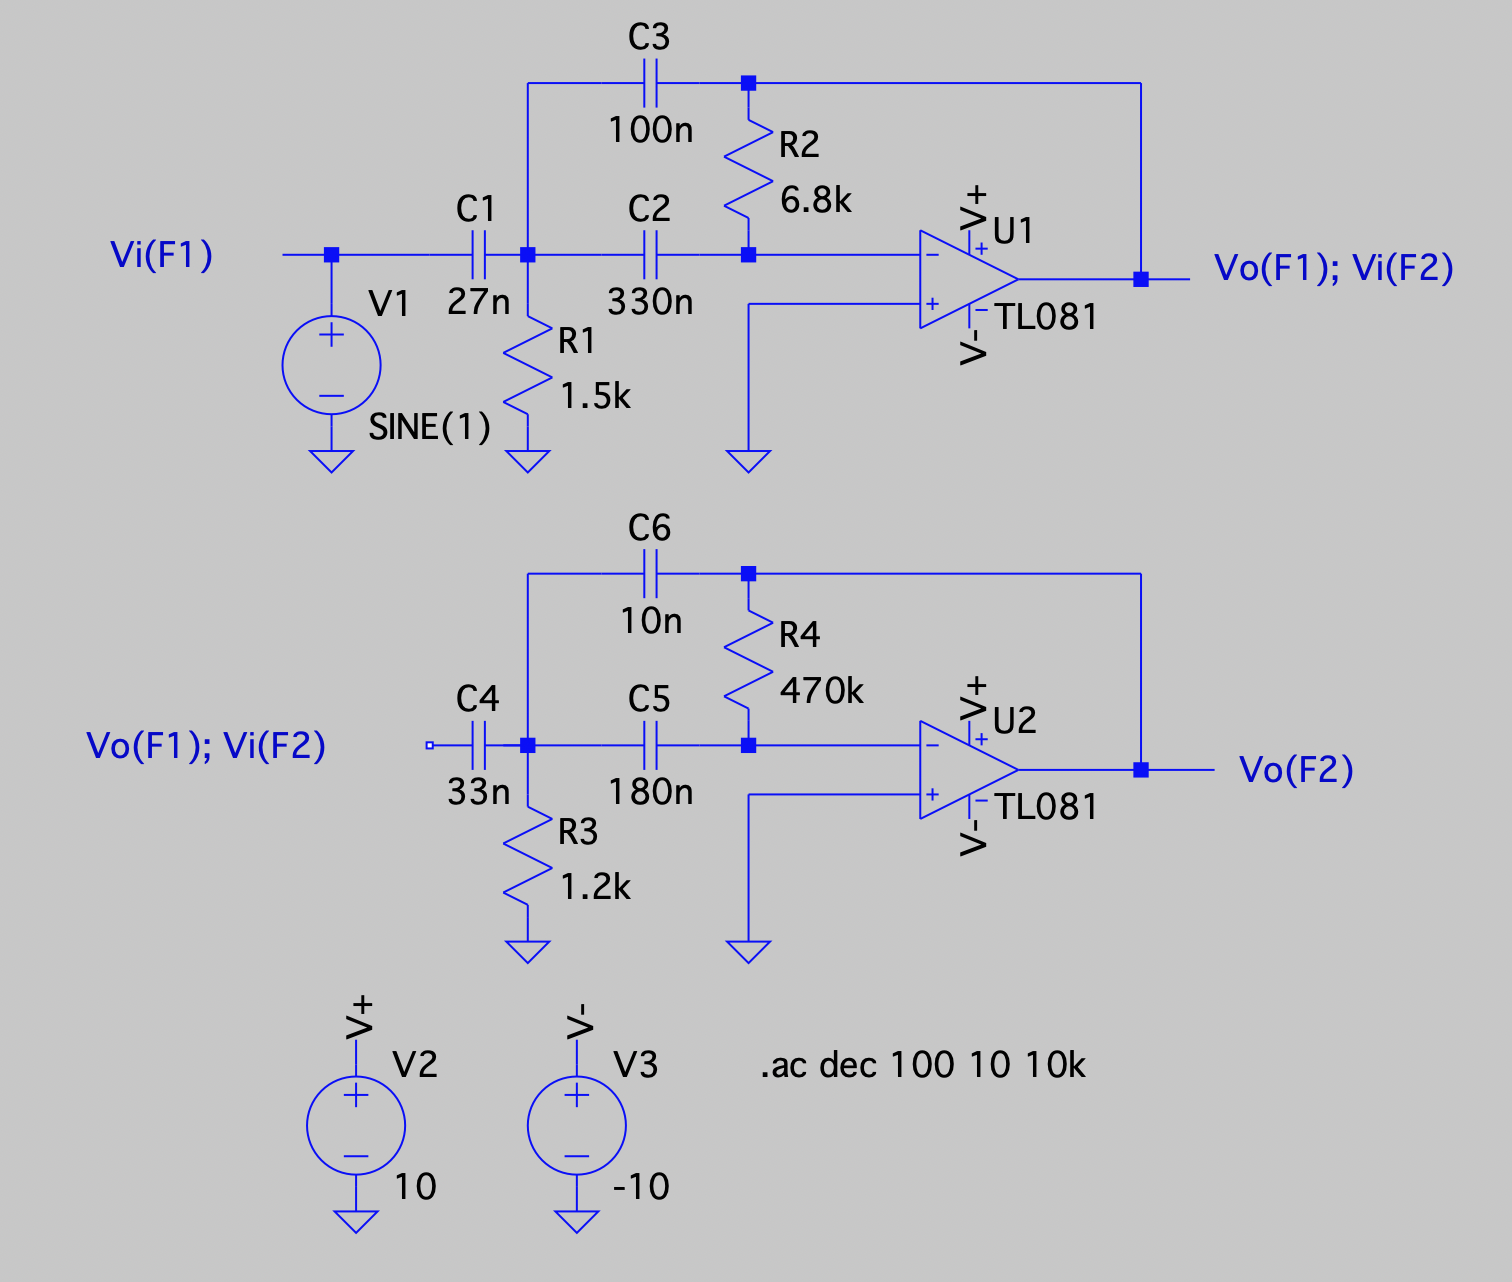
\includegraphics[width=1.1\textwidth,center]{images/ltspice/spice_complete_filter.png}}
        \caption{Simulación del filtro simulado con LTspice con componentes resistivos y capacitivos de la serie E24.}
        \label{fig}
    \end{figure}
    \subsubsection{Diagramas de Bode}

    \begin{figure}[H]
        \centering
        \scalebox{0.9}{%% Creator: Matplotlib, PGF backend
%%
%% To include the figure in your LaTeX document, write
%%   \input{<filename>.pgf}
%%
%% Make sure the required packages are loaded in your preamble
%%   \usepackage{pgf}
%%
%% and, on pdftex
%%   \usepackage[utf8]{inputenc}\DeclareUnicodeCharacter{2212}{-}
%%
%% or, on luatex and xetex
%%   \usepackage{unicode-math}
%%
%% Figures using additional raster images can only be included by \input if
%% they are in the same directory as the main LaTeX file. For loading figures
%% from other directories you can use the `import` package
%%   \usepackage{import}
%%
%% and then include the figures with
%%   \import{<path to file>}{<filename>.pgf}
%%
%% Matplotlib used the following preamble
%%   \usepackage{fontspec}
%%   \setmainfont{DejaVuSerif.ttf}[Path=/usr/local/lib/python3.7/site-packages/matplotlib/mpl-data/fonts/ttf/]
%%   \setsansfont{DejaVuSans.ttf}[Path=/usr/local/lib/python3.7/site-packages/matplotlib/mpl-data/fonts/ttf/]
%%   \setmonofont{DejaVuSansMono.ttf}[Path=/usr/local/lib/python3.7/site-packages/matplotlib/mpl-data/fonts/ttf/]
%%
\begingroup%
\makeatletter%
\begin{pgfpicture}%
\pgfpathrectangle{\pgfpointorigin}{\pgfqpoint{6.400000in}{4.800000in}}%
\pgfusepath{use as bounding box, clip}%
\begin{pgfscope}%
\pgfsetbuttcap%
\pgfsetmiterjoin%
\definecolor{currentfill}{rgb}{1.000000,1.000000,1.000000}%
\pgfsetfillcolor{currentfill}%
\pgfsetlinewidth{0.000000pt}%
\definecolor{currentstroke}{rgb}{1.000000,1.000000,1.000000}%
\pgfsetstrokecolor{currentstroke}%
\pgfsetdash{}{0pt}%
\pgfpathmoveto{\pgfqpoint{0.000000in}{0.000000in}}%
\pgfpathlineto{\pgfqpoint{6.400000in}{0.000000in}}%
\pgfpathlineto{\pgfqpoint{6.400000in}{4.800000in}}%
\pgfpathlineto{\pgfqpoint{0.000000in}{4.800000in}}%
\pgfpathclose%
\pgfusepath{fill}%
\end{pgfscope}%
\begin{pgfscope}%
\pgfsetbuttcap%
\pgfsetmiterjoin%
\definecolor{currentfill}{rgb}{1.000000,1.000000,1.000000}%
\pgfsetfillcolor{currentfill}%
\pgfsetlinewidth{0.000000pt}%
\definecolor{currentstroke}{rgb}{0.000000,0.000000,0.000000}%
\pgfsetstrokecolor{currentstroke}%
\pgfsetstrokeopacity{0.000000}%
\pgfsetdash{}{0pt}%
\pgfpathmoveto{\pgfqpoint{0.818660in}{0.571603in}}%
\pgfpathlineto{\pgfqpoint{5.581340in}{0.571603in}}%
\pgfpathlineto{\pgfqpoint{5.581340in}{4.440039in}}%
\pgfpathlineto{\pgfqpoint{0.818660in}{4.440039in}}%
\pgfpathclose%
\pgfusepath{fill}%
\end{pgfscope}%
\begin{pgfscope}%
\pgfsetbuttcap%
\pgfsetroundjoin%
\definecolor{currentfill}{rgb}{0.000000,0.000000,0.000000}%
\pgfsetfillcolor{currentfill}%
\pgfsetlinewidth{0.803000pt}%
\definecolor{currentstroke}{rgb}{0.000000,0.000000,0.000000}%
\pgfsetstrokecolor{currentstroke}%
\pgfsetdash{}{0pt}%
\pgfsys@defobject{currentmarker}{\pgfqpoint{0.000000in}{-0.048611in}}{\pgfqpoint{0.000000in}{0.000000in}}{%
\pgfpathmoveto{\pgfqpoint{0.000000in}{0.000000in}}%
\pgfpathlineto{\pgfqpoint{0.000000in}{-0.048611in}}%
\pgfusepath{stroke,fill}%
}%
\begin{pgfscope}%
\pgfsys@transformshift{1.035146in}{0.571603in}%
\pgfsys@useobject{currentmarker}{}%
\end{pgfscope}%
\end{pgfscope}%
\begin{pgfscope}%
\definecolor{textcolor}{rgb}{0.000000,0.000000,0.000000}%
\pgfsetstrokecolor{textcolor}%
\pgfsetfillcolor{textcolor}%
\pgftext[x=1.035146in,y=0.474381in,,top]{\color{textcolor}\sffamily\fontsize{10.000000}{12.000000}\selectfont \(\displaystyle {10^{1}}\)}%
\end{pgfscope}%
\begin{pgfscope}%
\pgfsetbuttcap%
\pgfsetroundjoin%
\definecolor{currentfill}{rgb}{0.000000,0.000000,0.000000}%
\pgfsetfillcolor{currentfill}%
\pgfsetlinewidth{0.803000pt}%
\definecolor{currentstroke}{rgb}{0.000000,0.000000,0.000000}%
\pgfsetstrokecolor{currentstroke}%
\pgfsetdash{}{0pt}%
\pgfsys@defobject{currentmarker}{\pgfqpoint{0.000000in}{-0.048611in}}{\pgfqpoint{0.000000in}{0.000000in}}{%
\pgfpathmoveto{\pgfqpoint{0.000000in}{0.000000in}}%
\pgfpathlineto{\pgfqpoint{0.000000in}{-0.048611in}}%
\pgfusepath{stroke,fill}%
}%
\begin{pgfscope}%
\pgfsys@transformshift{2.478382in}{0.571603in}%
\pgfsys@useobject{currentmarker}{}%
\end{pgfscope}%
\end{pgfscope}%
\begin{pgfscope}%
\definecolor{textcolor}{rgb}{0.000000,0.000000,0.000000}%
\pgfsetstrokecolor{textcolor}%
\pgfsetfillcolor{textcolor}%
\pgftext[x=2.478382in,y=0.474381in,,top]{\color{textcolor}\sffamily\fontsize{10.000000}{12.000000}\selectfont \(\displaystyle {10^{2}}\)}%
\end{pgfscope}%
\begin{pgfscope}%
\pgfsetbuttcap%
\pgfsetroundjoin%
\definecolor{currentfill}{rgb}{0.000000,0.000000,0.000000}%
\pgfsetfillcolor{currentfill}%
\pgfsetlinewidth{0.803000pt}%
\definecolor{currentstroke}{rgb}{0.000000,0.000000,0.000000}%
\pgfsetstrokecolor{currentstroke}%
\pgfsetdash{}{0pt}%
\pgfsys@defobject{currentmarker}{\pgfqpoint{0.000000in}{-0.048611in}}{\pgfqpoint{0.000000in}{0.000000in}}{%
\pgfpathmoveto{\pgfqpoint{0.000000in}{0.000000in}}%
\pgfpathlineto{\pgfqpoint{0.000000in}{-0.048611in}}%
\pgfusepath{stroke,fill}%
}%
\begin{pgfscope}%
\pgfsys@transformshift{3.921618in}{0.571603in}%
\pgfsys@useobject{currentmarker}{}%
\end{pgfscope}%
\end{pgfscope}%
\begin{pgfscope}%
\definecolor{textcolor}{rgb}{0.000000,0.000000,0.000000}%
\pgfsetstrokecolor{textcolor}%
\pgfsetfillcolor{textcolor}%
\pgftext[x=3.921618in,y=0.474381in,,top]{\color{textcolor}\sffamily\fontsize{10.000000}{12.000000}\selectfont \(\displaystyle {10^{3}}\)}%
\end{pgfscope}%
\begin{pgfscope}%
\pgfsetbuttcap%
\pgfsetroundjoin%
\definecolor{currentfill}{rgb}{0.000000,0.000000,0.000000}%
\pgfsetfillcolor{currentfill}%
\pgfsetlinewidth{0.803000pt}%
\definecolor{currentstroke}{rgb}{0.000000,0.000000,0.000000}%
\pgfsetstrokecolor{currentstroke}%
\pgfsetdash{}{0pt}%
\pgfsys@defobject{currentmarker}{\pgfqpoint{0.000000in}{-0.048611in}}{\pgfqpoint{0.000000in}{0.000000in}}{%
\pgfpathmoveto{\pgfqpoint{0.000000in}{0.000000in}}%
\pgfpathlineto{\pgfqpoint{0.000000in}{-0.048611in}}%
\pgfusepath{stroke,fill}%
}%
\begin{pgfscope}%
\pgfsys@transformshift{5.364854in}{0.571603in}%
\pgfsys@useobject{currentmarker}{}%
\end{pgfscope}%
\end{pgfscope}%
\begin{pgfscope}%
\definecolor{textcolor}{rgb}{0.000000,0.000000,0.000000}%
\pgfsetstrokecolor{textcolor}%
\pgfsetfillcolor{textcolor}%
\pgftext[x=5.364854in,y=0.474381in,,top]{\color{textcolor}\sffamily\fontsize{10.000000}{12.000000}\selectfont \(\displaystyle {10^{4}}\)}%
\end{pgfscope}%
\begin{pgfscope}%
\pgfsetbuttcap%
\pgfsetroundjoin%
\definecolor{currentfill}{rgb}{0.000000,0.000000,0.000000}%
\pgfsetfillcolor{currentfill}%
\pgfsetlinewidth{0.602250pt}%
\definecolor{currentstroke}{rgb}{0.000000,0.000000,0.000000}%
\pgfsetstrokecolor{currentstroke}%
\pgfsetdash{}{0pt}%
\pgfsys@defobject{currentmarker}{\pgfqpoint{0.000000in}{-0.027778in}}{\pgfqpoint{0.000000in}{0.000000in}}{%
\pgfpathmoveto{\pgfqpoint{0.000000in}{0.000000in}}%
\pgfpathlineto{\pgfqpoint{0.000000in}{-0.027778in}}%
\pgfusepath{stroke,fill}%
}%
\begin{pgfscope}%
\pgfsys@transformshift{0.895282in}{0.571603in}%
\pgfsys@useobject{currentmarker}{}%
\end{pgfscope}%
\end{pgfscope}%
\begin{pgfscope}%
\pgfsetbuttcap%
\pgfsetroundjoin%
\definecolor{currentfill}{rgb}{0.000000,0.000000,0.000000}%
\pgfsetfillcolor{currentfill}%
\pgfsetlinewidth{0.602250pt}%
\definecolor{currentstroke}{rgb}{0.000000,0.000000,0.000000}%
\pgfsetstrokecolor{currentstroke}%
\pgfsetdash{}{0pt}%
\pgfsys@defobject{currentmarker}{\pgfqpoint{0.000000in}{-0.027778in}}{\pgfqpoint{0.000000in}{0.000000in}}{%
\pgfpathmoveto{\pgfqpoint{0.000000in}{0.000000in}}%
\pgfpathlineto{\pgfqpoint{0.000000in}{-0.027778in}}%
\pgfusepath{stroke,fill}%
}%
\begin{pgfscope}%
\pgfsys@transformshift{0.969107in}{0.571603in}%
\pgfsys@useobject{currentmarker}{}%
\end{pgfscope}%
\end{pgfscope}%
\begin{pgfscope}%
\pgfsetbuttcap%
\pgfsetroundjoin%
\definecolor{currentfill}{rgb}{0.000000,0.000000,0.000000}%
\pgfsetfillcolor{currentfill}%
\pgfsetlinewidth{0.602250pt}%
\definecolor{currentstroke}{rgb}{0.000000,0.000000,0.000000}%
\pgfsetstrokecolor{currentstroke}%
\pgfsetdash{}{0pt}%
\pgfsys@defobject{currentmarker}{\pgfqpoint{0.000000in}{-0.027778in}}{\pgfqpoint{0.000000in}{0.000000in}}{%
\pgfpathmoveto{\pgfqpoint{0.000000in}{0.000000in}}%
\pgfpathlineto{\pgfqpoint{0.000000in}{-0.027778in}}%
\pgfusepath{stroke,fill}%
}%
\begin{pgfscope}%
\pgfsys@transformshift{1.469603in}{0.571603in}%
\pgfsys@useobject{currentmarker}{}%
\end{pgfscope}%
\end{pgfscope}%
\begin{pgfscope}%
\pgfsetbuttcap%
\pgfsetroundjoin%
\definecolor{currentfill}{rgb}{0.000000,0.000000,0.000000}%
\pgfsetfillcolor{currentfill}%
\pgfsetlinewidth{0.602250pt}%
\definecolor{currentstroke}{rgb}{0.000000,0.000000,0.000000}%
\pgfsetstrokecolor{currentstroke}%
\pgfsetdash{}{0pt}%
\pgfsys@defobject{currentmarker}{\pgfqpoint{0.000000in}{-0.027778in}}{\pgfqpoint{0.000000in}{0.000000in}}{%
\pgfpathmoveto{\pgfqpoint{0.000000in}{0.000000in}}%
\pgfpathlineto{\pgfqpoint{0.000000in}{-0.027778in}}%
\pgfusepath{stroke,fill}%
}%
\begin{pgfscope}%
\pgfsys@transformshift{1.723744in}{0.571603in}%
\pgfsys@useobject{currentmarker}{}%
\end{pgfscope}%
\end{pgfscope}%
\begin{pgfscope}%
\pgfsetbuttcap%
\pgfsetroundjoin%
\definecolor{currentfill}{rgb}{0.000000,0.000000,0.000000}%
\pgfsetfillcolor{currentfill}%
\pgfsetlinewidth{0.602250pt}%
\definecolor{currentstroke}{rgb}{0.000000,0.000000,0.000000}%
\pgfsetstrokecolor{currentstroke}%
\pgfsetdash{}{0pt}%
\pgfsys@defobject{currentmarker}{\pgfqpoint{0.000000in}{-0.027778in}}{\pgfqpoint{0.000000in}{0.000000in}}{%
\pgfpathmoveto{\pgfqpoint{0.000000in}{0.000000in}}%
\pgfpathlineto{\pgfqpoint{0.000000in}{-0.027778in}}%
\pgfusepath{stroke,fill}%
}%
\begin{pgfscope}%
\pgfsys@transformshift{1.904060in}{0.571603in}%
\pgfsys@useobject{currentmarker}{}%
\end{pgfscope}%
\end{pgfscope}%
\begin{pgfscope}%
\pgfsetbuttcap%
\pgfsetroundjoin%
\definecolor{currentfill}{rgb}{0.000000,0.000000,0.000000}%
\pgfsetfillcolor{currentfill}%
\pgfsetlinewidth{0.602250pt}%
\definecolor{currentstroke}{rgb}{0.000000,0.000000,0.000000}%
\pgfsetstrokecolor{currentstroke}%
\pgfsetdash{}{0pt}%
\pgfsys@defobject{currentmarker}{\pgfqpoint{0.000000in}{-0.027778in}}{\pgfqpoint{0.000000in}{0.000000in}}{%
\pgfpathmoveto{\pgfqpoint{0.000000in}{0.000000in}}%
\pgfpathlineto{\pgfqpoint{0.000000in}{-0.027778in}}%
\pgfusepath{stroke,fill}%
}%
\begin{pgfscope}%
\pgfsys@transformshift{2.043925in}{0.571603in}%
\pgfsys@useobject{currentmarker}{}%
\end{pgfscope}%
\end{pgfscope}%
\begin{pgfscope}%
\pgfsetbuttcap%
\pgfsetroundjoin%
\definecolor{currentfill}{rgb}{0.000000,0.000000,0.000000}%
\pgfsetfillcolor{currentfill}%
\pgfsetlinewidth{0.602250pt}%
\definecolor{currentstroke}{rgb}{0.000000,0.000000,0.000000}%
\pgfsetstrokecolor{currentstroke}%
\pgfsetdash{}{0pt}%
\pgfsys@defobject{currentmarker}{\pgfqpoint{0.000000in}{-0.027778in}}{\pgfqpoint{0.000000in}{0.000000in}}{%
\pgfpathmoveto{\pgfqpoint{0.000000in}{0.000000in}}%
\pgfpathlineto{\pgfqpoint{0.000000in}{-0.027778in}}%
\pgfusepath{stroke,fill}%
}%
\begin{pgfscope}%
\pgfsys@transformshift{2.158202in}{0.571603in}%
\pgfsys@useobject{currentmarker}{}%
\end{pgfscope}%
\end{pgfscope}%
\begin{pgfscope}%
\pgfsetbuttcap%
\pgfsetroundjoin%
\definecolor{currentfill}{rgb}{0.000000,0.000000,0.000000}%
\pgfsetfillcolor{currentfill}%
\pgfsetlinewidth{0.602250pt}%
\definecolor{currentstroke}{rgb}{0.000000,0.000000,0.000000}%
\pgfsetstrokecolor{currentstroke}%
\pgfsetdash{}{0pt}%
\pgfsys@defobject{currentmarker}{\pgfqpoint{0.000000in}{-0.027778in}}{\pgfqpoint{0.000000in}{0.000000in}}{%
\pgfpathmoveto{\pgfqpoint{0.000000in}{0.000000in}}%
\pgfpathlineto{\pgfqpoint{0.000000in}{-0.027778in}}%
\pgfusepath{stroke,fill}%
}%
\begin{pgfscope}%
\pgfsys@transformshift{2.254822in}{0.571603in}%
\pgfsys@useobject{currentmarker}{}%
\end{pgfscope}%
\end{pgfscope}%
\begin{pgfscope}%
\pgfsetbuttcap%
\pgfsetroundjoin%
\definecolor{currentfill}{rgb}{0.000000,0.000000,0.000000}%
\pgfsetfillcolor{currentfill}%
\pgfsetlinewidth{0.602250pt}%
\definecolor{currentstroke}{rgb}{0.000000,0.000000,0.000000}%
\pgfsetstrokecolor{currentstroke}%
\pgfsetdash{}{0pt}%
\pgfsys@defobject{currentmarker}{\pgfqpoint{0.000000in}{-0.027778in}}{\pgfqpoint{0.000000in}{0.000000in}}{%
\pgfpathmoveto{\pgfqpoint{0.000000in}{0.000000in}}%
\pgfpathlineto{\pgfqpoint{0.000000in}{-0.027778in}}%
\pgfusepath{stroke,fill}%
}%
\begin{pgfscope}%
\pgfsys@transformshift{2.338518in}{0.571603in}%
\pgfsys@useobject{currentmarker}{}%
\end{pgfscope}%
\end{pgfscope}%
\begin{pgfscope}%
\pgfsetbuttcap%
\pgfsetroundjoin%
\definecolor{currentfill}{rgb}{0.000000,0.000000,0.000000}%
\pgfsetfillcolor{currentfill}%
\pgfsetlinewidth{0.602250pt}%
\definecolor{currentstroke}{rgb}{0.000000,0.000000,0.000000}%
\pgfsetstrokecolor{currentstroke}%
\pgfsetdash{}{0pt}%
\pgfsys@defobject{currentmarker}{\pgfqpoint{0.000000in}{-0.027778in}}{\pgfqpoint{0.000000in}{0.000000in}}{%
\pgfpathmoveto{\pgfqpoint{0.000000in}{0.000000in}}%
\pgfpathlineto{\pgfqpoint{0.000000in}{-0.027778in}}%
\pgfusepath{stroke,fill}%
}%
\begin{pgfscope}%
\pgfsys@transformshift{2.412343in}{0.571603in}%
\pgfsys@useobject{currentmarker}{}%
\end{pgfscope}%
\end{pgfscope}%
\begin{pgfscope}%
\pgfsetbuttcap%
\pgfsetroundjoin%
\definecolor{currentfill}{rgb}{0.000000,0.000000,0.000000}%
\pgfsetfillcolor{currentfill}%
\pgfsetlinewidth{0.602250pt}%
\definecolor{currentstroke}{rgb}{0.000000,0.000000,0.000000}%
\pgfsetstrokecolor{currentstroke}%
\pgfsetdash{}{0pt}%
\pgfsys@defobject{currentmarker}{\pgfqpoint{0.000000in}{-0.027778in}}{\pgfqpoint{0.000000in}{0.000000in}}{%
\pgfpathmoveto{\pgfqpoint{0.000000in}{0.000000in}}%
\pgfpathlineto{\pgfqpoint{0.000000in}{-0.027778in}}%
\pgfusepath{stroke,fill}%
}%
\begin{pgfscope}%
\pgfsys@transformshift{2.912839in}{0.571603in}%
\pgfsys@useobject{currentmarker}{}%
\end{pgfscope}%
\end{pgfscope}%
\begin{pgfscope}%
\pgfsetbuttcap%
\pgfsetroundjoin%
\definecolor{currentfill}{rgb}{0.000000,0.000000,0.000000}%
\pgfsetfillcolor{currentfill}%
\pgfsetlinewidth{0.602250pt}%
\definecolor{currentstroke}{rgb}{0.000000,0.000000,0.000000}%
\pgfsetstrokecolor{currentstroke}%
\pgfsetdash{}{0pt}%
\pgfsys@defobject{currentmarker}{\pgfqpoint{0.000000in}{-0.027778in}}{\pgfqpoint{0.000000in}{0.000000in}}{%
\pgfpathmoveto{\pgfqpoint{0.000000in}{0.000000in}}%
\pgfpathlineto{\pgfqpoint{0.000000in}{-0.027778in}}%
\pgfusepath{stroke,fill}%
}%
\begin{pgfscope}%
\pgfsys@transformshift{3.166981in}{0.571603in}%
\pgfsys@useobject{currentmarker}{}%
\end{pgfscope}%
\end{pgfscope}%
\begin{pgfscope}%
\pgfsetbuttcap%
\pgfsetroundjoin%
\definecolor{currentfill}{rgb}{0.000000,0.000000,0.000000}%
\pgfsetfillcolor{currentfill}%
\pgfsetlinewidth{0.602250pt}%
\definecolor{currentstroke}{rgb}{0.000000,0.000000,0.000000}%
\pgfsetstrokecolor{currentstroke}%
\pgfsetdash{}{0pt}%
\pgfsys@defobject{currentmarker}{\pgfqpoint{0.000000in}{-0.027778in}}{\pgfqpoint{0.000000in}{0.000000in}}{%
\pgfpathmoveto{\pgfqpoint{0.000000in}{0.000000in}}%
\pgfpathlineto{\pgfqpoint{0.000000in}{-0.027778in}}%
\pgfusepath{stroke,fill}%
}%
\begin{pgfscope}%
\pgfsys@transformshift{3.347297in}{0.571603in}%
\pgfsys@useobject{currentmarker}{}%
\end{pgfscope}%
\end{pgfscope}%
\begin{pgfscope}%
\pgfsetbuttcap%
\pgfsetroundjoin%
\definecolor{currentfill}{rgb}{0.000000,0.000000,0.000000}%
\pgfsetfillcolor{currentfill}%
\pgfsetlinewidth{0.602250pt}%
\definecolor{currentstroke}{rgb}{0.000000,0.000000,0.000000}%
\pgfsetstrokecolor{currentstroke}%
\pgfsetdash{}{0pt}%
\pgfsys@defobject{currentmarker}{\pgfqpoint{0.000000in}{-0.027778in}}{\pgfqpoint{0.000000in}{0.000000in}}{%
\pgfpathmoveto{\pgfqpoint{0.000000in}{0.000000in}}%
\pgfpathlineto{\pgfqpoint{0.000000in}{-0.027778in}}%
\pgfusepath{stroke,fill}%
}%
\begin{pgfscope}%
\pgfsys@transformshift{3.487161in}{0.571603in}%
\pgfsys@useobject{currentmarker}{}%
\end{pgfscope}%
\end{pgfscope}%
\begin{pgfscope}%
\pgfsetbuttcap%
\pgfsetroundjoin%
\definecolor{currentfill}{rgb}{0.000000,0.000000,0.000000}%
\pgfsetfillcolor{currentfill}%
\pgfsetlinewidth{0.602250pt}%
\definecolor{currentstroke}{rgb}{0.000000,0.000000,0.000000}%
\pgfsetstrokecolor{currentstroke}%
\pgfsetdash{}{0pt}%
\pgfsys@defobject{currentmarker}{\pgfqpoint{0.000000in}{-0.027778in}}{\pgfqpoint{0.000000in}{0.000000in}}{%
\pgfpathmoveto{\pgfqpoint{0.000000in}{0.000000in}}%
\pgfpathlineto{\pgfqpoint{0.000000in}{-0.027778in}}%
\pgfusepath{stroke,fill}%
}%
\begin{pgfscope}%
\pgfsys@transformshift{3.601438in}{0.571603in}%
\pgfsys@useobject{currentmarker}{}%
\end{pgfscope}%
\end{pgfscope}%
\begin{pgfscope}%
\pgfsetbuttcap%
\pgfsetroundjoin%
\definecolor{currentfill}{rgb}{0.000000,0.000000,0.000000}%
\pgfsetfillcolor{currentfill}%
\pgfsetlinewidth{0.602250pt}%
\definecolor{currentstroke}{rgb}{0.000000,0.000000,0.000000}%
\pgfsetstrokecolor{currentstroke}%
\pgfsetdash{}{0pt}%
\pgfsys@defobject{currentmarker}{\pgfqpoint{0.000000in}{-0.027778in}}{\pgfqpoint{0.000000in}{0.000000in}}{%
\pgfpathmoveto{\pgfqpoint{0.000000in}{0.000000in}}%
\pgfpathlineto{\pgfqpoint{0.000000in}{-0.027778in}}%
\pgfusepath{stroke,fill}%
}%
\begin{pgfscope}%
\pgfsys@transformshift{3.698058in}{0.571603in}%
\pgfsys@useobject{currentmarker}{}%
\end{pgfscope}%
\end{pgfscope}%
\begin{pgfscope}%
\pgfsetbuttcap%
\pgfsetroundjoin%
\definecolor{currentfill}{rgb}{0.000000,0.000000,0.000000}%
\pgfsetfillcolor{currentfill}%
\pgfsetlinewidth{0.602250pt}%
\definecolor{currentstroke}{rgb}{0.000000,0.000000,0.000000}%
\pgfsetstrokecolor{currentstroke}%
\pgfsetdash{}{0pt}%
\pgfsys@defobject{currentmarker}{\pgfqpoint{0.000000in}{-0.027778in}}{\pgfqpoint{0.000000in}{0.000000in}}{%
\pgfpathmoveto{\pgfqpoint{0.000000in}{0.000000in}}%
\pgfpathlineto{\pgfqpoint{0.000000in}{-0.027778in}}%
\pgfusepath{stroke,fill}%
}%
\begin{pgfscope}%
\pgfsys@transformshift{3.781754in}{0.571603in}%
\pgfsys@useobject{currentmarker}{}%
\end{pgfscope}%
\end{pgfscope}%
\begin{pgfscope}%
\pgfsetbuttcap%
\pgfsetroundjoin%
\definecolor{currentfill}{rgb}{0.000000,0.000000,0.000000}%
\pgfsetfillcolor{currentfill}%
\pgfsetlinewidth{0.602250pt}%
\definecolor{currentstroke}{rgb}{0.000000,0.000000,0.000000}%
\pgfsetstrokecolor{currentstroke}%
\pgfsetdash{}{0pt}%
\pgfsys@defobject{currentmarker}{\pgfqpoint{0.000000in}{-0.027778in}}{\pgfqpoint{0.000000in}{0.000000in}}{%
\pgfpathmoveto{\pgfqpoint{0.000000in}{0.000000in}}%
\pgfpathlineto{\pgfqpoint{0.000000in}{-0.027778in}}%
\pgfusepath{stroke,fill}%
}%
\begin{pgfscope}%
\pgfsys@transformshift{3.855579in}{0.571603in}%
\pgfsys@useobject{currentmarker}{}%
\end{pgfscope}%
\end{pgfscope}%
\begin{pgfscope}%
\pgfsetbuttcap%
\pgfsetroundjoin%
\definecolor{currentfill}{rgb}{0.000000,0.000000,0.000000}%
\pgfsetfillcolor{currentfill}%
\pgfsetlinewidth{0.602250pt}%
\definecolor{currentstroke}{rgb}{0.000000,0.000000,0.000000}%
\pgfsetstrokecolor{currentstroke}%
\pgfsetdash{}{0pt}%
\pgfsys@defobject{currentmarker}{\pgfqpoint{0.000000in}{-0.027778in}}{\pgfqpoint{0.000000in}{0.000000in}}{%
\pgfpathmoveto{\pgfqpoint{0.000000in}{0.000000in}}%
\pgfpathlineto{\pgfqpoint{0.000000in}{-0.027778in}}%
\pgfusepath{stroke,fill}%
}%
\begin{pgfscope}%
\pgfsys@transformshift{4.356075in}{0.571603in}%
\pgfsys@useobject{currentmarker}{}%
\end{pgfscope}%
\end{pgfscope}%
\begin{pgfscope}%
\pgfsetbuttcap%
\pgfsetroundjoin%
\definecolor{currentfill}{rgb}{0.000000,0.000000,0.000000}%
\pgfsetfillcolor{currentfill}%
\pgfsetlinewidth{0.602250pt}%
\definecolor{currentstroke}{rgb}{0.000000,0.000000,0.000000}%
\pgfsetstrokecolor{currentstroke}%
\pgfsetdash{}{0pt}%
\pgfsys@defobject{currentmarker}{\pgfqpoint{0.000000in}{-0.027778in}}{\pgfqpoint{0.000000in}{0.000000in}}{%
\pgfpathmoveto{\pgfqpoint{0.000000in}{0.000000in}}%
\pgfpathlineto{\pgfqpoint{0.000000in}{-0.027778in}}%
\pgfusepath{stroke,fill}%
}%
\begin{pgfscope}%
\pgfsys@transformshift{4.610217in}{0.571603in}%
\pgfsys@useobject{currentmarker}{}%
\end{pgfscope}%
\end{pgfscope}%
\begin{pgfscope}%
\pgfsetbuttcap%
\pgfsetroundjoin%
\definecolor{currentfill}{rgb}{0.000000,0.000000,0.000000}%
\pgfsetfillcolor{currentfill}%
\pgfsetlinewidth{0.602250pt}%
\definecolor{currentstroke}{rgb}{0.000000,0.000000,0.000000}%
\pgfsetstrokecolor{currentstroke}%
\pgfsetdash{}{0pt}%
\pgfsys@defobject{currentmarker}{\pgfqpoint{0.000000in}{-0.027778in}}{\pgfqpoint{0.000000in}{0.000000in}}{%
\pgfpathmoveto{\pgfqpoint{0.000000in}{0.000000in}}%
\pgfpathlineto{\pgfqpoint{0.000000in}{-0.027778in}}%
\pgfusepath{stroke,fill}%
}%
\begin{pgfscope}%
\pgfsys@transformshift{4.790533in}{0.571603in}%
\pgfsys@useobject{currentmarker}{}%
\end{pgfscope}%
\end{pgfscope}%
\begin{pgfscope}%
\pgfsetbuttcap%
\pgfsetroundjoin%
\definecolor{currentfill}{rgb}{0.000000,0.000000,0.000000}%
\pgfsetfillcolor{currentfill}%
\pgfsetlinewidth{0.602250pt}%
\definecolor{currentstroke}{rgb}{0.000000,0.000000,0.000000}%
\pgfsetstrokecolor{currentstroke}%
\pgfsetdash{}{0pt}%
\pgfsys@defobject{currentmarker}{\pgfqpoint{0.000000in}{-0.027778in}}{\pgfqpoint{0.000000in}{0.000000in}}{%
\pgfpathmoveto{\pgfqpoint{0.000000in}{0.000000in}}%
\pgfpathlineto{\pgfqpoint{0.000000in}{-0.027778in}}%
\pgfusepath{stroke,fill}%
}%
\begin{pgfscope}%
\pgfsys@transformshift{4.930397in}{0.571603in}%
\pgfsys@useobject{currentmarker}{}%
\end{pgfscope}%
\end{pgfscope}%
\begin{pgfscope}%
\pgfsetbuttcap%
\pgfsetroundjoin%
\definecolor{currentfill}{rgb}{0.000000,0.000000,0.000000}%
\pgfsetfillcolor{currentfill}%
\pgfsetlinewidth{0.602250pt}%
\definecolor{currentstroke}{rgb}{0.000000,0.000000,0.000000}%
\pgfsetstrokecolor{currentstroke}%
\pgfsetdash{}{0pt}%
\pgfsys@defobject{currentmarker}{\pgfqpoint{0.000000in}{-0.027778in}}{\pgfqpoint{0.000000in}{0.000000in}}{%
\pgfpathmoveto{\pgfqpoint{0.000000in}{0.000000in}}%
\pgfpathlineto{\pgfqpoint{0.000000in}{-0.027778in}}%
\pgfusepath{stroke,fill}%
}%
\begin{pgfscope}%
\pgfsys@transformshift{5.044674in}{0.571603in}%
\pgfsys@useobject{currentmarker}{}%
\end{pgfscope}%
\end{pgfscope}%
\begin{pgfscope}%
\pgfsetbuttcap%
\pgfsetroundjoin%
\definecolor{currentfill}{rgb}{0.000000,0.000000,0.000000}%
\pgfsetfillcolor{currentfill}%
\pgfsetlinewidth{0.602250pt}%
\definecolor{currentstroke}{rgb}{0.000000,0.000000,0.000000}%
\pgfsetstrokecolor{currentstroke}%
\pgfsetdash{}{0pt}%
\pgfsys@defobject{currentmarker}{\pgfqpoint{0.000000in}{-0.027778in}}{\pgfqpoint{0.000000in}{0.000000in}}{%
\pgfpathmoveto{\pgfqpoint{0.000000in}{0.000000in}}%
\pgfpathlineto{\pgfqpoint{0.000000in}{-0.027778in}}%
\pgfusepath{stroke,fill}%
}%
\begin{pgfscope}%
\pgfsys@transformshift{5.141294in}{0.571603in}%
\pgfsys@useobject{currentmarker}{}%
\end{pgfscope}%
\end{pgfscope}%
\begin{pgfscope}%
\pgfsetbuttcap%
\pgfsetroundjoin%
\definecolor{currentfill}{rgb}{0.000000,0.000000,0.000000}%
\pgfsetfillcolor{currentfill}%
\pgfsetlinewidth{0.602250pt}%
\definecolor{currentstroke}{rgb}{0.000000,0.000000,0.000000}%
\pgfsetstrokecolor{currentstroke}%
\pgfsetdash{}{0pt}%
\pgfsys@defobject{currentmarker}{\pgfqpoint{0.000000in}{-0.027778in}}{\pgfqpoint{0.000000in}{0.000000in}}{%
\pgfpathmoveto{\pgfqpoint{0.000000in}{0.000000in}}%
\pgfpathlineto{\pgfqpoint{0.000000in}{-0.027778in}}%
\pgfusepath{stroke,fill}%
}%
\begin{pgfscope}%
\pgfsys@transformshift{5.224990in}{0.571603in}%
\pgfsys@useobject{currentmarker}{}%
\end{pgfscope}%
\end{pgfscope}%
\begin{pgfscope}%
\pgfsetbuttcap%
\pgfsetroundjoin%
\definecolor{currentfill}{rgb}{0.000000,0.000000,0.000000}%
\pgfsetfillcolor{currentfill}%
\pgfsetlinewidth{0.602250pt}%
\definecolor{currentstroke}{rgb}{0.000000,0.000000,0.000000}%
\pgfsetstrokecolor{currentstroke}%
\pgfsetdash{}{0pt}%
\pgfsys@defobject{currentmarker}{\pgfqpoint{0.000000in}{-0.027778in}}{\pgfqpoint{0.000000in}{0.000000in}}{%
\pgfpathmoveto{\pgfqpoint{0.000000in}{0.000000in}}%
\pgfpathlineto{\pgfqpoint{0.000000in}{-0.027778in}}%
\pgfusepath{stroke,fill}%
}%
\begin{pgfscope}%
\pgfsys@transformshift{5.298815in}{0.571603in}%
\pgfsys@useobject{currentmarker}{}%
\end{pgfscope}%
\end{pgfscope}%
\begin{pgfscope}%
\definecolor{textcolor}{rgb}{0.000000,0.000000,0.000000}%
\pgfsetstrokecolor{textcolor}%
\pgfsetfillcolor{textcolor}%
\pgftext[x=3.200000in,y=0.284413in,,top]{\color{textcolor}\sffamily\fontsize{10.000000}{12.000000}\selectfont \(\displaystyle \omega\) [rad/seg]\, (log)}%
\end{pgfscope}%
\begin{pgfscope}%
\pgfsetbuttcap%
\pgfsetroundjoin%
\definecolor{currentfill}{rgb}{0.000000,0.000000,0.000000}%
\pgfsetfillcolor{currentfill}%
\pgfsetlinewidth{0.803000pt}%
\definecolor{currentstroke}{rgb}{0.000000,0.000000,0.000000}%
\pgfsetstrokecolor{currentstroke}%
\pgfsetdash{}{0pt}%
\pgfsys@defobject{currentmarker}{\pgfqpoint{-0.048611in}{0.000000in}}{\pgfqpoint{0.000000in}{0.000000in}}{%
\pgfpathmoveto{\pgfqpoint{0.000000in}{0.000000in}}%
\pgfpathlineto{\pgfqpoint{-0.048611in}{0.000000in}}%
\pgfusepath{stroke,fill}%
}%
\begin{pgfscope}%
\pgfsys@transformshift{0.818660in}{0.956216in}%
\pgfsys@useobject{currentmarker}{}%
\end{pgfscope}%
\end{pgfscope}%
\begin{pgfscope}%
\definecolor{textcolor}{rgb}{1.000000,0.647059,0.000000}%
\pgfsetstrokecolor{textcolor}%
\pgfsetfillcolor{textcolor}%
\pgftext[x=0.339968in, y=0.903455in, left, base]{\color{textcolor}\sffamily\fontsize{10.000000}{12.000000}\selectfont −100}%
\end{pgfscope}%
\begin{pgfscope}%
\pgfsetbuttcap%
\pgfsetroundjoin%
\definecolor{currentfill}{rgb}{0.000000,0.000000,0.000000}%
\pgfsetfillcolor{currentfill}%
\pgfsetlinewidth{0.803000pt}%
\definecolor{currentstroke}{rgb}{0.000000,0.000000,0.000000}%
\pgfsetstrokecolor{currentstroke}%
\pgfsetdash{}{0pt}%
\pgfsys@defobject{currentmarker}{\pgfqpoint{-0.048611in}{0.000000in}}{\pgfqpoint{0.000000in}{0.000000in}}{%
\pgfpathmoveto{\pgfqpoint{0.000000in}{0.000000in}}%
\pgfpathlineto{\pgfqpoint{-0.048611in}{0.000000in}}%
\pgfusepath{stroke,fill}%
}%
\begin{pgfscope}%
\pgfsys@transformshift{0.818660in}{1.604832in}%
\pgfsys@useobject{currentmarker}{}%
\end{pgfscope}%
\end{pgfscope}%
\begin{pgfscope}%
\definecolor{textcolor}{rgb}{1.000000,0.647059,0.000000}%
\pgfsetstrokecolor{textcolor}%
\pgfsetfillcolor{textcolor}%
\pgftext[x=0.428334in, y=1.552070in, left, base]{\color{textcolor}\sffamily\fontsize{10.000000}{12.000000}\selectfont −80}%
\end{pgfscope}%
\begin{pgfscope}%
\pgfsetbuttcap%
\pgfsetroundjoin%
\definecolor{currentfill}{rgb}{0.000000,0.000000,0.000000}%
\pgfsetfillcolor{currentfill}%
\pgfsetlinewidth{0.803000pt}%
\definecolor{currentstroke}{rgb}{0.000000,0.000000,0.000000}%
\pgfsetstrokecolor{currentstroke}%
\pgfsetdash{}{0pt}%
\pgfsys@defobject{currentmarker}{\pgfqpoint{-0.048611in}{0.000000in}}{\pgfqpoint{0.000000in}{0.000000in}}{%
\pgfpathmoveto{\pgfqpoint{0.000000in}{0.000000in}}%
\pgfpathlineto{\pgfqpoint{-0.048611in}{0.000000in}}%
\pgfusepath{stroke,fill}%
}%
\begin{pgfscope}%
\pgfsys@transformshift{0.818660in}{2.253447in}%
\pgfsys@useobject{currentmarker}{}%
\end{pgfscope}%
\end{pgfscope}%
\begin{pgfscope}%
\definecolor{textcolor}{rgb}{1.000000,0.647059,0.000000}%
\pgfsetstrokecolor{textcolor}%
\pgfsetfillcolor{textcolor}%
\pgftext[x=0.428334in, y=2.200686in, left, base]{\color{textcolor}\sffamily\fontsize{10.000000}{12.000000}\selectfont −60}%
\end{pgfscope}%
\begin{pgfscope}%
\pgfsetbuttcap%
\pgfsetroundjoin%
\definecolor{currentfill}{rgb}{0.000000,0.000000,0.000000}%
\pgfsetfillcolor{currentfill}%
\pgfsetlinewidth{0.803000pt}%
\definecolor{currentstroke}{rgb}{0.000000,0.000000,0.000000}%
\pgfsetstrokecolor{currentstroke}%
\pgfsetdash{}{0pt}%
\pgfsys@defobject{currentmarker}{\pgfqpoint{-0.048611in}{0.000000in}}{\pgfqpoint{0.000000in}{0.000000in}}{%
\pgfpathmoveto{\pgfqpoint{0.000000in}{0.000000in}}%
\pgfpathlineto{\pgfqpoint{-0.048611in}{0.000000in}}%
\pgfusepath{stroke,fill}%
}%
\begin{pgfscope}%
\pgfsys@transformshift{0.818660in}{2.902062in}%
\pgfsys@useobject{currentmarker}{}%
\end{pgfscope}%
\end{pgfscope}%
\begin{pgfscope}%
\definecolor{textcolor}{rgb}{1.000000,0.647059,0.000000}%
\pgfsetstrokecolor{textcolor}%
\pgfsetfillcolor{textcolor}%
\pgftext[x=0.428334in, y=2.849301in, left, base]{\color{textcolor}\sffamily\fontsize{10.000000}{12.000000}\selectfont −40}%
\end{pgfscope}%
\begin{pgfscope}%
\pgfsetbuttcap%
\pgfsetroundjoin%
\definecolor{currentfill}{rgb}{0.000000,0.000000,0.000000}%
\pgfsetfillcolor{currentfill}%
\pgfsetlinewidth{0.803000pt}%
\definecolor{currentstroke}{rgb}{0.000000,0.000000,0.000000}%
\pgfsetstrokecolor{currentstroke}%
\pgfsetdash{}{0pt}%
\pgfsys@defobject{currentmarker}{\pgfqpoint{-0.048611in}{0.000000in}}{\pgfqpoint{0.000000in}{0.000000in}}{%
\pgfpathmoveto{\pgfqpoint{0.000000in}{0.000000in}}%
\pgfpathlineto{\pgfqpoint{-0.048611in}{0.000000in}}%
\pgfusepath{stroke,fill}%
}%
\begin{pgfscope}%
\pgfsys@transformshift{0.818660in}{3.550678in}%
\pgfsys@useobject{currentmarker}{}%
\end{pgfscope}%
\end{pgfscope}%
\begin{pgfscope}%
\definecolor{textcolor}{rgb}{1.000000,0.647059,0.000000}%
\pgfsetstrokecolor{textcolor}%
\pgfsetfillcolor{textcolor}%
\pgftext[x=0.428334in, y=3.497916in, left, base]{\color{textcolor}\sffamily\fontsize{10.000000}{12.000000}\selectfont −20}%
\end{pgfscope}%
\begin{pgfscope}%
\pgfsetbuttcap%
\pgfsetroundjoin%
\definecolor{currentfill}{rgb}{0.000000,0.000000,0.000000}%
\pgfsetfillcolor{currentfill}%
\pgfsetlinewidth{0.803000pt}%
\definecolor{currentstroke}{rgb}{0.000000,0.000000,0.000000}%
\pgfsetstrokecolor{currentstroke}%
\pgfsetdash{}{0pt}%
\pgfsys@defobject{currentmarker}{\pgfqpoint{-0.048611in}{0.000000in}}{\pgfqpoint{0.000000in}{0.000000in}}{%
\pgfpathmoveto{\pgfqpoint{0.000000in}{0.000000in}}%
\pgfpathlineto{\pgfqpoint{-0.048611in}{0.000000in}}%
\pgfusepath{stroke,fill}%
}%
\begin{pgfscope}%
\pgfsys@transformshift{0.818660in}{4.199293in}%
\pgfsys@useobject{currentmarker}{}%
\end{pgfscope}%
\end{pgfscope}%
\begin{pgfscope}%
\definecolor{textcolor}{rgb}{1.000000,0.647059,0.000000}%
\pgfsetstrokecolor{textcolor}%
\pgfsetfillcolor{textcolor}%
\pgftext[x=0.633073in, y=4.146532in, left, base]{\color{textcolor}\sffamily\fontsize{10.000000}{12.000000}\selectfont 0}%
\end{pgfscope}%
\begin{pgfscope}%
\definecolor{textcolor}{rgb}{1.000000,0.647059,0.000000}%
\pgfsetstrokecolor{textcolor}%
\pgfsetfillcolor{textcolor}%
\pgftext[x=0.284413in,y=2.505821in,,bottom,rotate=90.000000]{\color{textcolor}\sffamily\fontsize{10.000000}{12.000000}\selectfont Modulo [dB]}%
\end{pgfscope}%
\begin{pgfscope}%
\pgfpathrectangle{\pgfqpoint{0.818660in}{0.571603in}}{\pgfqpoint{4.762679in}{3.868436in}}%
\pgfusepath{clip}%
\pgfsetrectcap%
\pgfsetroundjoin%
\pgfsetlinewidth{2.509375pt}%
\definecolor{currentstroke}{rgb}{1.000000,0.647059,0.000000}%
\pgfsetstrokecolor{currentstroke}%
\pgfsetdash{}{0pt}%
\pgfpathmoveto{\pgfqpoint{1.035146in}{0.747441in}}%
\pgfpathlineto{\pgfqpoint{1.496981in}{1.581761in}}%
\pgfpathlineto{\pgfqpoint{1.742331in}{2.029206in}}%
\pgfpathlineto{\pgfqpoint{1.915520in}{2.349383in}}%
\pgfpathlineto{\pgfqpoint{2.045411in}{2.593843in}}%
\pgfpathlineto{\pgfqpoint{2.146438in}{2.788106in}}%
\pgfpathlineto{\pgfqpoint{2.233032in}{2.958898in}}%
\pgfpathlineto{\pgfqpoint{2.305194in}{3.105507in}}%
\pgfpathlineto{\pgfqpoint{2.377355in}{3.257560in}}%
\pgfpathlineto{\pgfqpoint{2.435085in}{3.384584in}}%
\pgfpathlineto{\pgfqpoint{2.478382in}{3.484050in}}%
\pgfpathlineto{\pgfqpoint{2.521679in}{3.588179in}}%
\pgfpathlineto{\pgfqpoint{2.564976in}{3.698249in}}%
\pgfpathlineto{\pgfqpoint{2.608273in}{3.815788in}}%
\pgfpathlineto{\pgfqpoint{2.651570in}{3.941935in}}%
\pgfpathlineto{\pgfqpoint{2.723732in}{4.157617in}}%
\pgfpathlineto{\pgfqpoint{2.738164in}{4.193722in}}%
\pgfpathlineto{\pgfqpoint{2.752597in}{4.223368in}}%
\pgfpathlineto{\pgfqpoint{2.767029in}{4.244997in}}%
\pgfpathlineto{\pgfqpoint{2.781462in}{4.258219in}}%
\pgfpathlineto{\pgfqpoint{2.795894in}{4.264003in}}%
\pgfpathlineto{\pgfqpoint{2.810326in}{4.264201in}}%
\pgfpathlineto{\pgfqpoint{2.824759in}{4.260832in}}%
\pgfpathlineto{\pgfqpoint{2.853623in}{4.249635in}}%
\pgfpathlineto{\pgfqpoint{2.882488in}{4.238343in}}%
\pgfpathlineto{\pgfqpoint{2.911353in}{4.229690in}}%
\pgfpathlineto{\pgfqpoint{2.940217in}{4.224074in}}%
\pgfpathlineto{\pgfqpoint{2.969082in}{4.221080in}}%
\pgfpathlineto{\pgfqpoint{2.997947in}{4.220079in}}%
\pgfpathlineto{\pgfqpoint{3.041244in}{4.220960in}}%
\pgfpathlineto{\pgfqpoint{3.185568in}{4.226906in}}%
\pgfpathlineto{\pgfqpoint{3.243297in}{4.226280in}}%
\pgfpathlineto{\pgfqpoint{3.301027in}{4.223555in}}%
\pgfpathlineto{\pgfqpoint{3.387621in}{4.216779in}}%
\pgfpathlineto{\pgfqpoint{3.676268in}{4.191366in}}%
\pgfpathlineto{\pgfqpoint{3.791727in}{4.184132in}}%
\pgfpathlineto{\pgfqpoint{3.921618in}{4.178196in}}%
\pgfpathlineto{\pgfqpoint{4.080374in}{4.173367in}}%
\pgfpathlineto{\pgfqpoint{4.267995in}{4.169968in}}%
\pgfpathlineto{\pgfqpoint{4.527777in}{4.167628in}}%
\pgfpathlineto{\pgfqpoint{4.917451in}{4.166561in}}%
\pgfpathlineto{\pgfqpoint{5.364854in}{4.167371in}}%
\pgfpathlineto{\pgfqpoint{5.364854in}{4.167371in}}%
\pgfusepath{stroke}%
\end{pgfscope}%
\begin{pgfscope}%
\pgfsetrectcap%
\pgfsetmiterjoin%
\pgfsetlinewidth{0.803000pt}%
\definecolor{currentstroke}{rgb}{0.000000,0.000000,0.000000}%
\pgfsetstrokecolor{currentstroke}%
\pgfsetdash{}{0pt}%
\pgfpathmoveto{\pgfqpoint{0.818660in}{0.571603in}}%
\pgfpathlineto{\pgfqpoint{0.818660in}{4.440039in}}%
\pgfusepath{stroke}%
\end{pgfscope}%
\begin{pgfscope}%
\pgfsetrectcap%
\pgfsetmiterjoin%
\pgfsetlinewidth{0.803000pt}%
\definecolor{currentstroke}{rgb}{0.000000,0.000000,0.000000}%
\pgfsetstrokecolor{currentstroke}%
\pgfsetdash{}{0pt}%
\pgfpathmoveto{\pgfqpoint{5.581340in}{0.571603in}}%
\pgfpathlineto{\pgfqpoint{5.581340in}{4.440039in}}%
\pgfusepath{stroke}%
\end{pgfscope}%
\begin{pgfscope}%
\pgfsetrectcap%
\pgfsetmiterjoin%
\pgfsetlinewidth{0.803000pt}%
\definecolor{currentstroke}{rgb}{0.000000,0.000000,0.000000}%
\pgfsetstrokecolor{currentstroke}%
\pgfsetdash{}{0pt}%
\pgfpathmoveto{\pgfqpoint{0.818660in}{0.571603in}}%
\pgfpathlineto{\pgfqpoint{5.581340in}{0.571603in}}%
\pgfusepath{stroke}%
\end{pgfscope}%
\begin{pgfscope}%
\pgfsetrectcap%
\pgfsetmiterjoin%
\pgfsetlinewidth{0.803000pt}%
\definecolor{currentstroke}{rgb}{0.000000,0.000000,0.000000}%
\pgfsetstrokecolor{currentstroke}%
\pgfsetdash{}{0pt}%
\pgfpathmoveto{\pgfqpoint{0.818660in}{4.440039in}}%
\pgfpathlineto{\pgfqpoint{5.581340in}{4.440039in}}%
\pgfusepath{stroke}%
\end{pgfscope}%
\begin{pgfscope}%
\definecolor{textcolor}{rgb}{0.000000,0.000000,0.000000}%
\pgfsetstrokecolor{textcolor}%
\pgfsetfillcolor{textcolor}%
\pgftext[x=3.200000in,y=4.523372in,,base]{\color{textcolor}\sffamily\fontsize{12.000000}{14.400000}\selectfont Diagrama real de Bode}%
\end{pgfscope}%
\begin{pgfscope}%
\pgfpathrectangle{\pgfqpoint{0.818660in}{0.571603in}}{\pgfqpoint{4.762679in}{3.868436in}}%
\pgfusepath{clip}%
\pgfsetrectcap%
\pgfsetroundjoin%
\pgfsetlinewidth{0.803000pt}%
\definecolor{currentstroke}{rgb}{0.690196,0.690196,0.690196}%
\pgfsetstrokecolor{currentstroke}%
\pgfsetdash{}{0pt}%
\pgfpathmoveto{\pgfqpoint{0.818660in}{0.835259in}}%
\pgfpathlineto{\pgfqpoint{5.581340in}{0.835259in}}%
\pgfusepath{stroke}%
\end{pgfscope}%
\begin{pgfscope}%
\pgfsetbuttcap%
\pgfsetroundjoin%
\definecolor{currentfill}{rgb}{0.000000,0.000000,0.000000}%
\pgfsetfillcolor{currentfill}%
\pgfsetlinewidth{0.803000pt}%
\definecolor{currentstroke}{rgb}{0.000000,0.000000,0.000000}%
\pgfsetstrokecolor{currentstroke}%
\pgfsetdash{}{0pt}%
\pgfsys@defobject{currentmarker}{\pgfqpoint{0.000000in}{0.000000in}}{\pgfqpoint{0.048611in}{0.000000in}}{%
\pgfpathmoveto{\pgfqpoint{0.000000in}{0.000000in}}%
\pgfpathlineto{\pgfqpoint{0.048611in}{0.000000in}}%
\pgfusepath{stroke,fill}%
}%
\begin{pgfscope}%
\pgfsys@transformshift{5.581340in}{0.835259in}%
\pgfsys@useobject{currentmarker}{}%
\end{pgfscope}%
\end{pgfscope}%
\begin{pgfscope}%
\definecolor{textcolor}{rgb}{0.254902,0.411765,0.882353}%
\pgfsetstrokecolor{textcolor}%
\pgfsetfillcolor{textcolor}%
\pgftext[x=5.678562in, y=0.782498in, left, base]{\color{textcolor}\sffamily\fontsize{10.000000}{12.000000}\selectfont −350}%
\end{pgfscope}%
\begin{pgfscope}%
\pgfpathrectangle{\pgfqpoint{0.818660in}{0.571603in}}{\pgfqpoint{4.762679in}{3.868436in}}%
\pgfusepath{clip}%
\pgfsetrectcap%
\pgfsetroundjoin%
\pgfsetlinewidth{0.803000pt}%
\definecolor{currentstroke}{rgb}{0.690196,0.690196,0.690196}%
\pgfsetstrokecolor{currentstroke}%
\pgfsetdash{}{0pt}%
\pgfpathmoveto{\pgfqpoint{0.818660in}{1.329968in}}%
\pgfpathlineto{\pgfqpoint{5.581340in}{1.329968in}}%
\pgfusepath{stroke}%
\end{pgfscope}%
\begin{pgfscope}%
\pgfsetbuttcap%
\pgfsetroundjoin%
\definecolor{currentfill}{rgb}{0.000000,0.000000,0.000000}%
\pgfsetfillcolor{currentfill}%
\pgfsetlinewidth{0.803000pt}%
\definecolor{currentstroke}{rgb}{0.000000,0.000000,0.000000}%
\pgfsetstrokecolor{currentstroke}%
\pgfsetdash{}{0pt}%
\pgfsys@defobject{currentmarker}{\pgfqpoint{0.000000in}{0.000000in}}{\pgfqpoint{0.048611in}{0.000000in}}{%
\pgfpathmoveto{\pgfqpoint{0.000000in}{0.000000in}}%
\pgfpathlineto{\pgfqpoint{0.048611in}{0.000000in}}%
\pgfusepath{stroke,fill}%
}%
\begin{pgfscope}%
\pgfsys@transformshift{5.581340in}{1.329968in}%
\pgfsys@useobject{currentmarker}{}%
\end{pgfscope}%
\end{pgfscope}%
\begin{pgfscope}%
\definecolor{textcolor}{rgb}{0.254902,0.411765,0.882353}%
\pgfsetstrokecolor{textcolor}%
\pgfsetfillcolor{textcolor}%
\pgftext[x=5.678562in, y=1.277207in, left, base]{\color{textcolor}\sffamily\fontsize{10.000000}{12.000000}\selectfont −300}%
\end{pgfscope}%
\begin{pgfscope}%
\pgfpathrectangle{\pgfqpoint{0.818660in}{0.571603in}}{\pgfqpoint{4.762679in}{3.868436in}}%
\pgfusepath{clip}%
\pgfsetrectcap%
\pgfsetroundjoin%
\pgfsetlinewidth{0.803000pt}%
\definecolor{currentstroke}{rgb}{0.690196,0.690196,0.690196}%
\pgfsetstrokecolor{currentstroke}%
\pgfsetdash{}{0pt}%
\pgfpathmoveto{\pgfqpoint{0.818660in}{1.824677in}}%
\pgfpathlineto{\pgfqpoint{5.581340in}{1.824677in}}%
\pgfusepath{stroke}%
\end{pgfscope}%
\begin{pgfscope}%
\pgfsetbuttcap%
\pgfsetroundjoin%
\definecolor{currentfill}{rgb}{0.000000,0.000000,0.000000}%
\pgfsetfillcolor{currentfill}%
\pgfsetlinewidth{0.803000pt}%
\definecolor{currentstroke}{rgb}{0.000000,0.000000,0.000000}%
\pgfsetstrokecolor{currentstroke}%
\pgfsetdash{}{0pt}%
\pgfsys@defobject{currentmarker}{\pgfqpoint{0.000000in}{0.000000in}}{\pgfqpoint{0.048611in}{0.000000in}}{%
\pgfpathmoveto{\pgfqpoint{0.000000in}{0.000000in}}%
\pgfpathlineto{\pgfqpoint{0.048611in}{0.000000in}}%
\pgfusepath{stroke,fill}%
}%
\begin{pgfscope}%
\pgfsys@transformshift{5.581340in}{1.824677in}%
\pgfsys@useobject{currentmarker}{}%
\end{pgfscope}%
\end{pgfscope}%
\begin{pgfscope}%
\definecolor{textcolor}{rgb}{0.254902,0.411765,0.882353}%
\pgfsetstrokecolor{textcolor}%
\pgfsetfillcolor{textcolor}%
\pgftext[x=5.678562in, y=1.771916in, left, base]{\color{textcolor}\sffamily\fontsize{10.000000}{12.000000}\selectfont −250}%
\end{pgfscope}%
\begin{pgfscope}%
\pgfpathrectangle{\pgfqpoint{0.818660in}{0.571603in}}{\pgfqpoint{4.762679in}{3.868436in}}%
\pgfusepath{clip}%
\pgfsetrectcap%
\pgfsetroundjoin%
\pgfsetlinewidth{0.803000pt}%
\definecolor{currentstroke}{rgb}{0.690196,0.690196,0.690196}%
\pgfsetstrokecolor{currentstroke}%
\pgfsetdash{}{0pt}%
\pgfpathmoveto{\pgfqpoint{0.818660in}{2.319386in}}%
\pgfpathlineto{\pgfqpoint{5.581340in}{2.319386in}}%
\pgfusepath{stroke}%
\end{pgfscope}%
\begin{pgfscope}%
\pgfsetbuttcap%
\pgfsetroundjoin%
\definecolor{currentfill}{rgb}{0.000000,0.000000,0.000000}%
\pgfsetfillcolor{currentfill}%
\pgfsetlinewidth{0.803000pt}%
\definecolor{currentstroke}{rgb}{0.000000,0.000000,0.000000}%
\pgfsetstrokecolor{currentstroke}%
\pgfsetdash{}{0pt}%
\pgfsys@defobject{currentmarker}{\pgfqpoint{0.000000in}{0.000000in}}{\pgfqpoint{0.048611in}{0.000000in}}{%
\pgfpathmoveto{\pgfqpoint{0.000000in}{0.000000in}}%
\pgfpathlineto{\pgfqpoint{0.048611in}{0.000000in}}%
\pgfusepath{stroke,fill}%
}%
\begin{pgfscope}%
\pgfsys@transformshift{5.581340in}{2.319386in}%
\pgfsys@useobject{currentmarker}{}%
\end{pgfscope}%
\end{pgfscope}%
\begin{pgfscope}%
\definecolor{textcolor}{rgb}{0.254902,0.411765,0.882353}%
\pgfsetstrokecolor{textcolor}%
\pgfsetfillcolor{textcolor}%
\pgftext[x=5.678562in, y=2.266624in, left, base]{\color{textcolor}\sffamily\fontsize{10.000000}{12.000000}\selectfont −200}%
\end{pgfscope}%
\begin{pgfscope}%
\pgfpathrectangle{\pgfqpoint{0.818660in}{0.571603in}}{\pgfqpoint{4.762679in}{3.868436in}}%
\pgfusepath{clip}%
\pgfsetrectcap%
\pgfsetroundjoin%
\pgfsetlinewidth{0.803000pt}%
\definecolor{currentstroke}{rgb}{0.690196,0.690196,0.690196}%
\pgfsetstrokecolor{currentstroke}%
\pgfsetdash{}{0pt}%
\pgfpathmoveto{\pgfqpoint{0.818660in}{2.814095in}}%
\pgfpathlineto{\pgfqpoint{5.581340in}{2.814095in}}%
\pgfusepath{stroke}%
\end{pgfscope}%
\begin{pgfscope}%
\pgfsetbuttcap%
\pgfsetroundjoin%
\definecolor{currentfill}{rgb}{0.000000,0.000000,0.000000}%
\pgfsetfillcolor{currentfill}%
\pgfsetlinewidth{0.803000pt}%
\definecolor{currentstroke}{rgb}{0.000000,0.000000,0.000000}%
\pgfsetstrokecolor{currentstroke}%
\pgfsetdash{}{0pt}%
\pgfsys@defobject{currentmarker}{\pgfqpoint{0.000000in}{0.000000in}}{\pgfqpoint{0.048611in}{0.000000in}}{%
\pgfpathmoveto{\pgfqpoint{0.000000in}{0.000000in}}%
\pgfpathlineto{\pgfqpoint{0.048611in}{0.000000in}}%
\pgfusepath{stroke,fill}%
}%
\begin{pgfscope}%
\pgfsys@transformshift{5.581340in}{2.814095in}%
\pgfsys@useobject{currentmarker}{}%
\end{pgfscope}%
\end{pgfscope}%
\begin{pgfscope}%
\definecolor{textcolor}{rgb}{0.254902,0.411765,0.882353}%
\pgfsetstrokecolor{textcolor}%
\pgfsetfillcolor{textcolor}%
\pgftext[x=5.678562in, y=2.761333in, left, base]{\color{textcolor}\sffamily\fontsize{10.000000}{12.000000}\selectfont −150}%
\end{pgfscope}%
\begin{pgfscope}%
\pgfpathrectangle{\pgfqpoint{0.818660in}{0.571603in}}{\pgfqpoint{4.762679in}{3.868436in}}%
\pgfusepath{clip}%
\pgfsetrectcap%
\pgfsetroundjoin%
\pgfsetlinewidth{0.803000pt}%
\definecolor{currentstroke}{rgb}{0.690196,0.690196,0.690196}%
\pgfsetstrokecolor{currentstroke}%
\pgfsetdash{}{0pt}%
\pgfpathmoveto{\pgfqpoint{0.818660in}{3.308804in}}%
\pgfpathlineto{\pgfqpoint{5.581340in}{3.308804in}}%
\pgfusepath{stroke}%
\end{pgfscope}%
\begin{pgfscope}%
\pgfsetbuttcap%
\pgfsetroundjoin%
\definecolor{currentfill}{rgb}{0.000000,0.000000,0.000000}%
\pgfsetfillcolor{currentfill}%
\pgfsetlinewidth{0.803000pt}%
\definecolor{currentstroke}{rgb}{0.000000,0.000000,0.000000}%
\pgfsetstrokecolor{currentstroke}%
\pgfsetdash{}{0pt}%
\pgfsys@defobject{currentmarker}{\pgfqpoint{0.000000in}{0.000000in}}{\pgfqpoint{0.048611in}{0.000000in}}{%
\pgfpathmoveto{\pgfqpoint{0.000000in}{0.000000in}}%
\pgfpathlineto{\pgfqpoint{0.048611in}{0.000000in}}%
\pgfusepath{stroke,fill}%
}%
\begin{pgfscope}%
\pgfsys@transformshift{5.581340in}{3.308804in}%
\pgfsys@useobject{currentmarker}{}%
\end{pgfscope}%
\end{pgfscope}%
\begin{pgfscope}%
\definecolor{textcolor}{rgb}{0.254902,0.411765,0.882353}%
\pgfsetstrokecolor{textcolor}%
\pgfsetfillcolor{textcolor}%
\pgftext[x=5.678562in, y=3.256042in, left, base]{\color{textcolor}\sffamily\fontsize{10.000000}{12.000000}\selectfont −100}%
\end{pgfscope}%
\begin{pgfscope}%
\pgfpathrectangle{\pgfqpoint{0.818660in}{0.571603in}}{\pgfqpoint{4.762679in}{3.868436in}}%
\pgfusepath{clip}%
\pgfsetrectcap%
\pgfsetroundjoin%
\pgfsetlinewidth{0.803000pt}%
\definecolor{currentstroke}{rgb}{0.690196,0.690196,0.690196}%
\pgfsetstrokecolor{currentstroke}%
\pgfsetdash{}{0pt}%
\pgfpathmoveto{\pgfqpoint{0.818660in}{3.803513in}}%
\pgfpathlineto{\pgfqpoint{5.581340in}{3.803513in}}%
\pgfusepath{stroke}%
\end{pgfscope}%
\begin{pgfscope}%
\pgfsetbuttcap%
\pgfsetroundjoin%
\definecolor{currentfill}{rgb}{0.000000,0.000000,0.000000}%
\pgfsetfillcolor{currentfill}%
\pgfsetlinewidth{0.803000pt}%
\definecolor{currentstroke}{rgb}{0.000000,0.000000,0.000000}%
\pgfsetstrokecolor{currentstroke}%
\pgfsetdash{}{0pt}%
\pgfsys@defobject{currentmarker}{\pgfqpoint{0.000000in}{0.000000in}}{\pgfqpoint{0.048611in}{0.000000in}}{%
\pgfpathmoveto{\pgfqpoint{0.000000in}{0.000000in}}%
\pgfpathlineto{\pgfqpoint{0.048611in}{0.000000in}}%
\pgfusepath{stroke,fill}%
}%
\begin{pgfscope}%
\pgfsys@transformshift{5.581340in}{3.803513in}%
\pgfsys@useobject{currentmarker}{}%
\end{pgfscope}%
\end{pgfscope}%
\begin{pgfscope}%
\definecolor{textcolor}{rgb}{0.254902,0.411765,0.882353}%
\pgfsetstrokecolor{textcolor}%
\pgfsetfillcolor{textcolor}%
\pgftext[x=5.678562in, y=3.750751in, left, base]{\color{textcolor}\sffamily\fontsize{10.000000}{12.000000}\selectfont −50}%
\end{pgfscope}%
\begin{pgfscope}%
\pgfpathrectangle{\pgfqpoint{0.818660in}{0.571603in}}{\pgfqpoint{4.762679in}{3.868436in}}%
\pgfusepath{clip}%
\pgfsetrectcap%
\pgfsetroundjoin%
\pgfsetlinewidth{0.803000pt}%
\definecolor{currentstroke}{rgb}{0.690196,0.690196,0.690196}%
\pgfsetstrokecolor{currentstroke}%
\pgfsetdash{}{0pt}%
\pgfpathmoveto{\pgfqpoint{0.818660in}{4.298221in}}%
\pgfpathlineto{\pgfqpoint{5.581340in}{4.298221in}}%
\pgfusepath{stroke}%
\end{pgfscope}%
\begin{pgfscope}%
\pgfsetbuttcap%
\pgfsetroundjoin%
\definecolor{currentfill}{rgb}{0.000000,0.000000,0.000000}%
\pgfsetfillcolor{currentfill}%
\pgfsetlinewidth{0.803000pt}%
\definecolor{currentstroke}{rgb}{0.000000,0.000000,0.000000}%
\pgfsetstrokecolor{currentstroke}%
\pgfsetdash{}{0pt}%
\pgfsys@defobject{currentmarker}{\pgfqpoint{0.000000in}{0.000000in}}{\pgfqpoint{0.048611in}{0.000000in}}{%
\pgfpathmoveto{\pgfqpoint{0.000000in}{0.000000in}}%
\pgfpathlineto{\pgfqpoint{0.048611in}{0.000000in}}%
\pgfusepath{stroke,fill}%
}%
\begin{pgfscope}%
\pgfsys@transformshift{5.581340in}{4.298221in}%
\pgfsys@useobject{currentmarker}{}%
\end{pgfscope}%
\end{pgfscope}%
\begin{pgfscope}%
\definecolor{textcolor}{rgb}{0.254902,0.411765,0.882353}%
\pgfsetstrokecolor{textcolor}%
\pgfsetfillcolor{textcolor}%
\pgftext[x=5.678562in, y=4.245460in, left, base]{\color{textcolor}\sffamily\fontsize{10.000000}{12.000000}\selectfont 0}%
\end{pgfscope}%
\begin{pgfscope}%
\definecolor{textcolor}{rgb}{0.254902,0.411765,0.882353}%
\pgfsetstrokecolor{textcolor}%
\pgfsetfillcolor{textcolor}%
\pgftext[x=6.115587in,y=2.505821in,,top,rotate=90.000000]{\color{textcolor}\sffamily\fontsize{10.000000}{12.000000}\selectfont Fase [rad]}%
\end{pgfscope}%
\begin{pgfscope}%
\pgfpathrectangle{\pgfqpoint{0.818660in}{0.571603in}}{\pgfqpoint{4.762679in}{3.868436in}}%
\pgfusepath{clip}%
\pgfsetrectcap%
\pgfsetroundjoin%
\pgfsetlinewidth{2.509375pt}%
\definecolor{currentstroke}{rgb}{0.254902,0.411765,0.882353}%
\pgfsetstrokecolor{currentstroke}%
\pgfsetdash{}{0pt}%
\pgfpathmoveto{\pgfqpoint{1.035146in}{4.264201in}}%
\pgfpathlineto{\pgfqpoint{1.193902in}{4.254348in}}%
\pgfpathlineto{\pgfqpoint{1.323793in}{4.244170in}}%
\pgfpathlineto{\pgfqpoint{1.439252in}{4.233119in}}%
\pgfpathlineto{\pgfqpoint{1.554711in}{4.219743in}}%
\pgfpathlineto{\pgfqpoint{1.655737in}{4.205712in}}%
\pgfpathlineto{\pgfqpoint{1.742331in}{4.191598in}}%
\pgfpathlineto{\pgfqpoint{1.828926in}{4.175174in}}%
\pgfpathlineto{\pgfqpoint{1.901087in}{4.159391in}}%
\pgfpathlineto{\pgfqpoint{1.973249in}{4.141341in}}%
\pgfpathlineto{\pgfqpoint{2.030979in}{4.124981in}}%
\pgfpathlineto{\pgfqpoint{2.088708in}{4.106608in}}%
\pgfpathlineto{\pgfqpoint{2.146438in}{4.085860in}}%
\pgfpathlineto{\pgfqpoint{2.204167in}{4.062265in}}%
\pgfpathlineto{\pgfqpoint{2.247464in}{4.042326in}}%
\pgfpathlineto{\pgfqpoint{2.290761in}{4.020077in}}%
\pgfpathlineto{\pgfqpoint{2.334058in}{3.995049in}}%
\pgfpathlineto{\pgfqpoint{2.377355in}{3.966610in}}%
\pgfpathlineto{\pgfqpoint{2.406220in}{3.945330in}}%
\pgfpathlineto{\pgfqpoint{2.435085in}{3.921793in}}%
\pgfpathlineto{\pgfqpoint{2.463950in}{3.895532in}}%
\pgfpathlineto{\pgfqpoint{2.492814in}{3.865923in}}%
\pgfpathlineto{\pgfqpoint{2.521679in}{3.832107in}}%
\pgfpathlineto{\pgfqpoint{2.550544in}{3.792863in}}%
\pgfpathlineto{\pgfqpoint{2.564976in}{3.770680in}}%
\pgfpathlineto{\pgfqpoint{2.579408in}{3.746412in}}%
\pgfpathlineto{\pgfqpoint{2.593841in}{3.719695in}}%
\pgfpathlineto{\pgfqpoint{2.608273in}{3.690075in}}%
\pgfpathlineto{\pgfqpoint{2.622706in}{3.656984in}}%
\pgfpathlineto{\pgfqpoint{2.637138in}{3.619715in}}%
\pgfpathlineto{\pgfqpoint{2.651570in}{3.577387in}}%
\pgfpathlineto{\pgfqpoint{2.666003in}{3.528919in}}%
\pgfpathlineto{\pgfqpoint{2.680435in}{3.473025in}}%
\pgfpathlineto{\pgfqpoint{2.694867in}{3.408273in}}%
\pgfpathlineto{\pgfqpoint{2.709300in}{3.333269in}}%
\pgfpathlineto{\pgfqpoint{2.723732in}{3.247072in}}%
\pgfpathlineto{\pgfqpoint{2.738164in}{3.149871in}}%
\pgfpathlineto{\pgfqpoint{2.767029in}{2.932950in}}%
\pgfpathlineto{\pgfqpoint{2.795894in}{2.719062in}}%
\pgfpathlineto{\pgfqpoint{2.810326in}{2.624391in}}%
\pgfpathlineto{\pgfqpoint{2.824759in}{2.540138in}}%
\pgfpathlineto{\pgfqpoint{2.839191in}{2.465884in}}%
\pgfpathlineto{\pgfqpoint{2.853623in}{2.400416in}}%
\pgfpathlineto{\pgfqpoint{2.868056in}{2.342295in}}%
\pgfpathlineto{\pgfqpoint{2.882488in}{2.290152in}}%
\pgfpathlineto{\pgfqpoint{2.896920in}{2.242805in}}%
\pgfpathlineto{\pgfqpoint{2.925785in}{2.158798in}}%
\pgfpathlineto{\pgfqpoint{2.954650in}{2.084618in}}%
\pgfpathlineto{\pgfqpoint{2.983515in}{2.016733in}}%
\pgfpathlineto{\pgfqpoint{3.026812in}{1.922234in}}%
\pgfpathlineto{\pgfqpoint{3.070109in}{1.833318in}}%
\pgfpathlineto{\pgfqpoint{3.113406in}{1.748486in}}%
\pgfpathlineto{\pgfqpoint{3.156703in}{1.667523in}}%
\pgfpathlineto{\pgfqpoint{3.200000in}{1.590812in}}%
\pgfpathlineto{\pgfqpoint{3.243297in}{1.518897in}}%
\pgfpathlineto{\pgfqpoint{3.286594in}{1.452215in}}%
\pgfpathlineto{\pgfqpoint{3.329891in}{1.390976in}}%
\pgfpathlineto{\pgfqpoint{3.373188in}{1.335155in}}%
\pgfpathlineto{\pgfqpoint{3.416485in}{1.284531in}}%
\pgfpathlineto{\pgfqpoint{3.459783in}{1.238755in}}%
\pgfpathlineto{\pgfqpoint{3.503080in}{1.197414in}}%
\pgfpathlineto{\pgfqpoint{3.546377in}{1.160074in}}%
\pgfpathlineto{\pgfqpoint{3.589674in}{1.126310in}}%
\pgfpathlineto{\pgfqpoint{3.632971in}{1.095730in}}%
\pgfpathlineto{\pgfqpoint{3.676268in}{1.067974in}}%
\pgfpathlineto{\pgfqpoint{3.719565in}{1.042726in}}%
\pgfpathlineto{\pgfqpoint{3.762862in}{1.019704in}}%
\pgfpathlineto{\pgfqpoint{3.820592in}{0.992054in}}%
\pgfpathlineto{\pgfqpoint{3.878321in}{0.967437in}}%
\pgfpathlineto{\pgfqpoint{3.936050in}{0.945440in}}%
\pgfpathlineto{\pgfqpoint{3.993780in}{0.925722in}}%
\pgfpathlineto{\pgfqpoint{4.065942in}{0.903844in}}%
\pgfpathlineto{\pgfqpoint{4.138104in}{0.884615in}}%
\pgfpathlineto{\pgfqpoint{4.210265in}{0.867657in}}%
\pgfpathlineto{\pgfqpoint{4.296860in}{0.849866in}}%
\pgfpathlineto{\pgfqpoint{4.383454in}{0.834452in}}%
\pgfpathlineto{\pgfqpoint{4.484480in}{0.818988in}}%
\pgfpathlineto{\pgfqpoint{4.585507in}{0.805791in}}%
\pgfpathlineto{\pgfqpoint{4.700966in}{0.792991in}}%
\pgfpathlineto{\pgfqpoint{4.830857in}{0.780939in}}%
\pgfpathlineto{\pgfqpoint{4.975181in}{0.769825in}}%
\pgfpathlineto{\pgfqpoint{5.148369in}{0.758827in}}%
\pgfpathlineto{\pgfqpoint{5.364854in}{0.747441in}}%
\pgfpathlineto{\pgfqpoint{5.364854in}{0.747441in}}%
\pgfusepath{stroke}%
\end{pgfscope}%
\begin{pgfscope}%
\pgfsetrectcap%
\pgfsetmiterjoin%
\pgfsetlinewidth{0.803000pt}%
\definecolor{currentstroke}{rgb}{0.000000,0.000000,0.000000}%
\pgfsetstrokecolor{currentstroke}%
\pgfsetdash{}{0pt}%
\pgfpathmoveto{\pgfqpoint{0.818660in}{0.571603in}}%
\pgfpathlineto{\pgfqpoint{0.818660in}{4.440039in}}%
\pgfusepath{stroke}%
\end{pgfscope}%
\begin{pgfscope}%
\pgfsetrectcap%
\pgfsetmiterjoin%
\pgfsetlinewidth{0.803000pt}%
\definecolor{currentstroke}{rgb}{0.000000,0.000000,0.000000}%
\pgfsetstrokecolor{currentstroke}%
\pgfsetdash{}{0pt}%
\pgfpathmoveto{\pgfqpoint{5.581340in}{0.571603in}}%
\pgfpathlineto{\pgfqpoint{5.581340in}{4.440039in}}%
\pgfusepath{stroke}%
\end{pgfscope}%
\begin{pgfscope}%
\pgfsetrectcap%
\pgfsetmiterjoin%
\pgfsetlinewidth{0.803000pt}%
\definecolor{currentstroke}{rgb}{0.000000,0.000000,0.000000}%
\pgfsetstrokecolor{currentstroke}%
\pgfsetdash{}{0pt}%
\pgfpathmoveto{\pgfqpoint{0.818660in}{0.571603in}}%
\pgfpathlineto{\pgfqpoint{5.581340in}{0.571603in}}%
\pgfusepath{stroke}%
\end{pgfscope}%
\begin{pgfscope}%
\pgfsetrectcap%
\pgfsetmiterjoin%
\pgfsetlinewidth{0.803000pt}%
\definecolor{currentstroke}{rgb}{0.000000,0.000000,0.000000}%
\pgfsetstrokecolor{currentstroke}%
\pgfsetdash{}{0pt}%
\pgfpathmoveto{\pgfqpoint{0.818660in}{4.440039in}}%
\pgfpathlineto{\pgfqpoint{5.581340in}{4.440039in}}%
\pgfusepath{stroke}%
\end{pgfscope}%
\end{pgfpicture}%
\makeatother%
\endgroup%
}
        \caption{Diagrama de Bode del filtro simulado con LTspice.}
        \label{fig}
    \end{figure}

    \begin{figure}[H]
        \centering
        \scalebox{0.9}{%% Creator: Matplotlib, PGF backend
%%
%% To include the figure in your LaTeX document, write
%%   \input{<filename>.pgf}
%%
%% Make sure the required packages are loaded in your preamble
%%   \usepackage{pgf}
%%
%% and, on pdftex
%%   \usepackage[utf8]{inputenc}\DeclareUnicodeCharacter{2212}{-}
%%
%% or, on luatex and xetex
%%   \usepackage{unicode-math}
%%
%% Figures using additional raster images can only be included by \input if
%% they are in the same directory as the main LaTeX file. For loading figures
%% from other directories you can use the `import` package
%%   \usepackage{import}
%%
%% and then include the figures with
%%   \import{<path to file>}{<filename>.pgf}
%%
%% Matplotlib used the following preamble
%%   \usepackage{fontspec}
%%   \setmainfont{DejaVuSerif.ttf}[Path=/usr/local/lib/python3.7/site-packages/matplotlib/mpl-data/fonts/ttf/]
%%   \setsansfont{DejaVuSans.ttf}[Path=/usr/local/lib/python3.7/site-packages/matplotlib/mpl-data/fonts/ttf/]
%%   \setmonofont{DejaVuSansMono.ttf}[Path=/usr/local/lib/python3.7/site-packages/matplotlib/mpl-data/fonts/ttf/]
%%
\begingroup%
\makeatletter%
\begin{pgfpicture}%
\pgfpathrectangle{\pgfpointorigin}{\pgfqpoint{6.400000in}{4.800000in}}%
\pgfusepath{use as bounding box, clip}%
\begin{pgfscope}%
\pgfsetbuttcap%
\pgfsetmiterjoin%
\definecolor{currentfill}{rgb}{1.000000,1.000000,1.000000}%
\pgfsetfillcolor{currentfill}%
\pgfsetlinewidth{0.000000pt}%
\definecolor{currentstroke}{rgb}{1.000000,1.000000,1.000000}%
\pgfsetstrokecolor{currentstroke}%
\pgfsetdash{}{0pt}%
\pgfpathmoveto{\pgfqpoint{0.000000in}{0.000000in}}%
\pgfpathlineto{\pgfqpoint{6.400000in}{0.000000in}}%
\pgfpathlineto{\pgfqpoint{6.400000in}{4.800000in}}%
\pgfpathlineto{\pgfqpoint{0.000000in}{4.800000in}}%
\pgfpathclose%
\pgfusepath{fill}%
\end{pgfscope}%
\begin{pgfscope}%
\pgfsetbuttcap%
\pgfsetmiterjoin%
\definecolor{currentfill}{rgb}{1.000000,1.000000,1.000000}%
\pgfsetfillcolor{currentfill}%
\pgfsetlinewidth{0.000000pt}%
\definecolor{currentstroke}{rgb}{0.000000,0.000000,0.000000}%
\pgfsetstrokecolor{currentstroke}%
\pgfsetstrokeopacity{0.000000}%
\pgfsetdash{}{0pt}%
\pgfpathmoveto{\pgfqpoint{0.774444in}{0.571603in}}%
\pgfpathlineto{\pgfqpoint{5.581340in}{0.571603in}}%
\pgfpathlineto{\pgfqpoint{5.581340in}{4.440039in}}%
\pgfpathlineto{\pgfqpoint{0.774444in}{4.440039in}}%
\pgfpathclose%
\pgfusepath{fill}%
\end{pgfscope}%
\begin{pgfscope}%
\pgfsetbuttcap%
\pgfsetroundjoin%
\definecolor{currentfill}{rgb}{0.000000,0.000000,0.000000}%
\pgfsetfillcolor{currentfill}%
\pgfsetlinewidth{0.803000pt}%
\definecolor{currentstroke}{rgb}{0.000000,0.000000,0.000000}%
\pgfsetstrokecolor{currentstroke}%
\pgfsetdash{}{0pt}%
\pgfsys@defobject{currentmarker}{\pgfqpoint{0.000000in}{-0.048611in}}{\pgfqpoint{0.000000in}{0.000000in}}{%
\pgfpathmoveto{\pgfqpoint{0.000000in}{0.000000in}}%
\pgfpathlineto{\pgfqpoint{0.000000in}{-0.048611in}}%
\pgfusepath{stroke,fill}%
}%
\begin{pgfscope}%
\pgfsys@transformshift{0.774444in}{0.571603in}%
\pgfsys@useobject{currentmarker}{}%
\end{pgfscope}%
\end{pgfscope}%
\begin{pgfscope}%
\definecolor{textcolor}{rgb}{0.000000,0.000000,0.000000}%
\pgfsetstrokecolor{textcolor}%
\pgfsetfillcolor{textcolor}%
\pgftext[x=0.774444in,y=0.474381in,,top]{\color{textcolor}\sffamily\fontsize{10.000000}{12.000000}\selectfont \(\displaystyle {10^{2}}\)}%
\end{pgfscope}%
\begin{pgfscope}%
\pgfsetbuttcap%
\pgfsetroundjoin%
\definecolor{currentfill}{rgb}{0.000000,0.000000,0.000000}%
\pgfsetfillcolor{currentfill}%
\pgfsetlinewidth{0.803000pt}%
\definecolor{currentstroke}{rgb}{0.000000,0.000000,0.000000}%
\pgfsetstrokecolor{currentstroke}%
\pgfsetdash{}{0pt}%
\pgfsys@defobject{currentmarker}{\pgfqpoint{0.000000in}{-0.048611in}}{\pgfqpoint{0.000000in}{0.000000in}}{%
\pgfpathmoveto{\pgfqpoint{0.000000in}{0.000000in}}%
\pgfpathlineto{\pgfqpoint{0.000000in}{-0.048611in}}%
\pgfusepath{stroke,fill}%
}%
\begin{pgfscope}%
\pgfsys@transformshift{5.581340in}{0.571603in}%
\pgfsys@useobject{currentmarker}{}%
\end{pgfscope}%
\end{pgfscope}%
\begin{pgfscope}%
\definecolor{textcolor}{rgb}{0.000000,0.000000,0.000000}%
\pgfsetstrokecolor{textcolor}%
\pgfsetfillcolor{textcolor}%
\pgftext[x=5.581340in,y=0.474381in,,top]{\color{textcolor}\sffamily\fontsize{10.000000}{12.000000}\selectfont \(\displaystyle {10^{3}}\)}%
\end{pgfscope}%
\begin{pgfscope}%
\pgfsetbuttcap%
\pgfsetroundjoin%
\definecolor{currentfill}{rgb}{0.000000,0.000000,0.000000}%
\pgfsetfillcolor{currentfill}%
\pgfsetlinewidth{0.602250pt}%
\definecolor{currentstroke}{rgb}{0.000000,0.000000,0.000000}%
\pgfsetstrokecolor{currentstroke}%
\pgfsetdash{}{0pt}%
\pgfsys@defobject{currentmarker}{\pgfqpoint{0.000000in}{-0.027778in}}{\pgfqpoint{0.000000in}{0.000000in}}{%
\pgfpathmoveto{\pgfqpoint{0.000000in}{0.000000in}}%
\pgfpathlineto{\pgfqpoint{0.000000in}{-0.027778in}}%
\pgfusepath{stroke,fill}%
}%
\begin{pgfscope}%
\pgfsys@transformshift{2.221464in}{0.571603in}%
\pgfsys@useobject{currentmarker}{}%
\end{pgfscope}%
\end{pgfscope}%
\begin{pgfscope}%
\definecolor{textcolor}{rgb}{0.000000,0.000000,0.000000}%
\pgfsetstrokecolor{textcolor}%
\pgfsetfillcolor{textcolor}%
\pgftext[x=2.221464in,y=0.496603in,,top]{\color{textcolor}\sffamily\fontsize{10.000000}{12.000000}\selectfont \(\displaystyle {2\times10^{2}}\)}%
\end{pgfscope}%
\begin{pgfscope}%
\pgfsetbuttcap%
\pgfsetroundjoin%
\definecolor{currentfill}{rgb}{0.000000,0.000000,0.000000}%
\pgfsetfillcolor{currentfill}%
\pgfsetlinewidth{0.602250pt}%
\definecolor{currentstroke}{rgb}{0.000000,0.000000,0.000000}%
\pgfsetstrokecolor{currentstroke}%
\pgfsetdash{}{0pt}%
\pgfsys@defobject{currentmarker}{\pgfqpoint{0.000000in}{-0.027778in}}{\pgfqpoint{0.000000in}{0.000000in}}{%
\pgfpathmoveto{\pgfqpoint{0.000000in}{0.000000in}}%
\pgfpathlineto{\pgfqpoint{0.000000in}{-0.027778in}}%
\pgfusepath{stroke,fill}%
}%
\begin{pgfscope}%
\pgfsys@transformshift{3.067916in}{0.571603in}%
\pgfsys@useobject{currentmarker}{}%
\end{pgfscope}%
\end{pgfscope}%
\begin{pgfscope}%
\definecolor{textcolor}{rgb}{0.000000,0.000000,0.000000}%
\pgfsetstrokecolor{textcolor}%
\pgfsetfillcolor{textcolor}%
\pgftext[x=3.067916in,y=0.496603in,,top]{\color{textcolor}\sffamily\fontsize{10.000000}{12.000000}\selectfont \(\displaystyle {3\times10^{2}}\)}%
\end{pgfscope}%
\begin{pgfscope}%
\pgfsetbuttcap%
\pgfsetroundjoin%
\definecolor{currentfill}{rgb}{0.000000,0.000000,0.000000}%
\pgfsetfillcolor{currentfill}%
\pgfsetlinewidth{0.602250pt}%
\definecolor{currentstroke}{rgb}{0.000000,0.000000,0.000000}%
\pgfsetstrokecolor{currentstroke}%
\pgfsetdash{}{0pt}%
\pgfsys@defobject{currentmarker}{\pgfqpoint{0.000000in}{-0.027778in}}{\pgfqpoint{0.000000in}{0.000000in}}{%
\pgfpathmoveto{\pgfqpoint{0.000000in}{0.000000in}}%
\pgfpathlineto{\pgfqpoint{0.000000in}{-0.027778in}}%
\pgfusepath{stroke,fill}%
}%
\begin{pgfscope}%
\pgfsys@transformshift{3.668483in}{0.571603in}%
\pgfsys@useobject{currentmarker}{}%
\end{pgfscope}%
\end{pgfscope}%
\begin{pgfscope}%
\definecolor{textcolor}{rgb}{0.000000,0.000000,0.000000}%
\pgfsetstrokecolor{textcolor}%
\pgfsetfillcolor{textcolor}%
\pgftext[x=3.668483in,y=0.496603in,,top]{\color{textcolor}\sffamily\fontsize{10.000000}{12.000000}\selectfont \(\displaystyle {4\times10^{2}}\)}%
\end{pgfscope}%
\begin{pgfscope}%
\pgfsetbuttcap%
\pgfsetroundjoin%
\definecolor{currentfill}{rgb}{0.000000,0.000000,0.000000}%
\pgfsetfillcolor{currentfill}%
\pgfsetlinewidth{0.602250pt}%
\definecolor{currentstroke}{rgb}{0.000000,0.000000,0.000000}%
\pgfsetstrokecolor{currentstroke}%
\pgfsetdash{}{0pt}%
\pgfsys@defobject{currentmarker}{\pgfqpoint{0.000000in}{-0.027778in}}{\pgfqpoint{0.000000in}{0.000000in}}{%
\pgfpathmoveto{\pgfqpoint{0.000000in}{0.000000in}}%
\pgfpathlineto{\pgfqpoint{0.000000in}{-0.027778in}}%
\pgfusepath{stroke,fill}%
}%
\begin{pgfscope}%
\pgfsys@transformshift{4.134320in}{0.571603in}%
\pgfsys@useobject{currentmarker}{}%
\end{pgfscope}%
\end{pgfscope}%
\begin{pgfscope}%
\pgfsetbuttcap%
\pgfsetroundjoin%
\definecolor{currentfill}{rgb}{0.000000,0.000000,0.000000}%
\pgfsetfillcolor{currentfill}%
\pgfsetlinewidth{0.602250pt}%
\definecolor{currentstroke}{rgb}{0.000000,0.000000,0.000000}%
\pgfsetstrokecolor{currentstroke}%
\pgfsetdash{}{0pt}%
\pgfsys@defobject{currentmarker}{\pgfqpoint{0.000000in}{-0.027778in}}{\pgfqpoint{0.000000in}{0.000000in}}{%
\pgfpathmoveto{\pgfqpoint{0.000000in}{0.000000in}}%
\pgfpathlineto{\pgfqpoint{0.000000in}{-0.027778in}}%
\pgfusepath{stroke,fill}%
}%
\begin{pgfscope}%
\pgfsys@transformshift{4.514936in}{0.571603in}%
\pgfsys@useobject{currentmarker}{}%
\end{pgfscope}%
\end{pgfscope}%
\begin{pgfscope}%
\definecolor{textcolor}{rgb}{0.000000,0.000000,0.000000}%
\pgfsetstrokecolor{textcolor}%
\pgfsetfillcolor{textcolor}%
\pgftext[x=4.514936in,y=0.496603in,,top]{\color{textcolor}\sffamily\fontsize{10.000000}{12.000000}\selectfont \(\displaystyle {6\times10^{2}}\)}%
\end{pgfscope}%
\begin{pgfscope}%
\pgfsetbuttcap%
\pgfsetroundjoin%
\definecolor{currentfill}{rgb}{0.000000,0.000000,0.000000}%
\pgfsetfillcolor{currentfill}%
\pgfsetlinewidth{0.602250pt}%
\definecolor{currentstroke}{rgb}{0.000000,0.000000,0.000000}%
\pgfsetstrokecolor{currentstroke}%
\pgfsetdash{}{0pt}%
\pgfsys@defobject{currentmarker}{\pgfqpoint{0.000000in}{-0.027778in}}{\pgfqpoint{0.000000in}{0.000000in}}{%
\pgfpathmoveto{\pgfqpoint{0.000000in}{0.000000in}}%
\pgfpathlineto{\pgfqpoint{0.000000in}{-0.027778in}}%
\pgfusepath{stroke,fill}%
}%
\begin{pgfscope}%
\pgfsys@transformshift{4.836742in}{0.571603in}%
\pgfsys@useobject{currentmarker}{}%
\end{pgfscope}%
\end{pgfscope}%
\begin{pgfscope}%
\pgfsetbuttcap%
\pgfsetroundjoin%
\definecolor{currentfill}{rgb}{0.000000,0.000000,0.000000}%
\pgfsetfillcolor{currentfill}%
\pgfsetlinewidth{0.602250pt}%
\definecolor{currentstroke}{rgb}{0.000000,0.000000,0.000000}%
\pgfsetstrokecolor{currentstroke}%
\pgfsetdash{}{0pt}%
\pgfsys@defobject{currentmarker}{\pgfqpoint{0.000000in}{-0.027778in}}{\pgfqpoint{0.000000in}{0.000000in}}{%
\pgfpathmoveto{\pgfqpoint{0.000000in}{0.000000in}}%
\pgfpathlineto{\pgfqpoint{0.000000in}{-0.027778in}}%
\pgfusepath{stroke,fill}%
}%
\begin{pgfscope}%
\pgfsys@transformshift{5.115503in}{0.571603in}%
\pgfsys@useobject{currentmarker}{}%
\end{pgfscope}%
\end{pgfscope}%
\begin{pgfscope}%
\pgfsetbuttcap%
\pgfsetroundjoin%
\definecolor{currentfill}{rgb}{0.000000,0.000000,0.000000}%
\pgfsetfillcolor{currentfill}%
\pgfsetlinewidth{0.602250pt}%
\definecolor{currentstroke}{rgb}{0.000000,0.000000,0.000000}%
\pgfsetstrokecolor{currentstroke}%
\pgfsetdash{}{0pt}%
\pgfsys@defobject{currentmarker}{\pgfqpoint{0.000000in}{-0.027778in}}{\pgfqpoint{0.000000in}{0.000000in}}{%
\pgfpathmoveto{\pgfqpoint{0.000000in}{0.000000in}}%
\pgfpathlineto{\pgfqpoint{0.000000in}{-0.027778in}}%
\pgfusepath{stroke,fill}%
}%
\begin{pgfscope}%
\pgfsys@transformshift{5.361388in}{0.571603in}%
\pgfsys@useobject{currentmarker}{}%
\end{pgfscope}%
\end{pgfscope}%
\begin{pgfscope}%
\definecolor{textcolor}{rgb}{0.000000,0.000000,0.000000}%
\pgfsetstrokecolor{textcolor}%
\pgfsetfillcolor{textcolor}%
\pgftext[x=3.177892in,y=0.284413in,,top]{\color{textcolor}\sffamily\fontsize{10.000000}{12.000000}\selectfont \(\displaystyle \omega\) [rad/seg]\, (log)}%
\end{pgfscope}%
\begin{pgfscope}%
\pgfsetbuttcap%
\pgfsetroundjoin%
\definecolor{currentfill}{rgb}{0.000000,0.000000,0.000000}%
\pgfsetfillcolor{currentfill}%
\pgfsetlinewidth{0.803000pt}%
\definecolor{currentstroke}{rgb}{0.000000,0.000000,0.000000}%
\pgfsetstrokecolor{currentstroke}%
\pgfsetdash{}{0pt}%
\pgfsys@defobject{currentmarker}{\pgfqpoint{-0.048611in}{0.000000in}}{\pgfqpoint{0.000000in}{0.000000in}}{%
\pgfpathmoveto{\pgfqpoint{0.000000in}{0.000000in}}%
\pgfpathlineto{\pgfqpoint{-0.048611in}{0.000000in}}%
\pgfusepath{stroke,fill}%
}%
\begin{pgfscope}%
\pgfsys@transformshift{0.774444in}{0.877006in}%
\pgfsys@useobject{currentmarker}{}%
\end{pgfscope}%
\end{pgfscope}%
\begin{pgfscope}%
\definecolor{textcolor}{rgb}{1.000000,0.647059,0.000000}%
\pgfsetstrokecolor{textcolor}%
\pgfsetfillcolor{textcolor}%
\pgftext[x=0.339968in, y=0.824245in, left, base]{\color{textcolor}\sffamily\fontsize{10.000000}{12.000000}\selectfont −1.0}%
\end{pgfscope}%
\begin{pgfscope}%
\pgfsetbuttcap%
\pgfsetroundjoin%
\definecolor{currentfill}{rgb}{0.000000,0.000000,0.000000}%
\pgfsetfillcolor{currentfill}%
\pgfsetlinewidth{0.803000pt}%
\definecolor{currentstroke}{rgb}{0.000000,0.000000,0.000000}%
\pgfsetstrokecolor{currentstroke}%
\pgfsetdash{}{0pt}%
\pgfsys@defobject{currentmarker}{\pgfqpoint{-0.048611in}{0.000000in}}{\pgfqpoint{0.000000in}{0.000000in}}{%
\pgfpathmoveto{\pgfqpoint{0.000000in}{0.000000in}}%
\pgfpathlineto{\pgfqpoint{-0.048611in}{0.000000in}}%
\pgfusepath{stroke,fill}%
}%
\begin{pgfscope}%
\pgfsys@transformshift{0.774444in}{1.386011in}%
\pgfsys@useobject{currentmarker}{}%
\end{pgfscope}%
\end{pgfscope}%
\begin{pgfscope}%
\definecolor{textcolor}{rgb}{1.000000,0.647059,0.000000}%
\pgfsetstrokecolor{textcolor}%
\pgfsetfillcolor{textcolor}%
\pgftext[x=0.339968in, y=1.333249in, left, base]{\color{textcolor}\sffamily\fontsize{10.000000}{12.000000}\selectfont −0.5}%
\end{pgfscope}%
\begin{pgfscope}%
\pgfsetbuttcap%
\pgfsetroundjoin%
\definecolor{currentfill}{rgb}{0.000000,0.000000,0.000000}%
\pgfsetfillcolor{currentfill}%
\pgfsetlinewidth{0.803000pt}%
\definecolor{currentstroke}{rgb}{0.000000,0.000000,0.000000}%
\pgfsetstrokecolor{currentstroke}%
\pgfsetdash{}{0pt}%
\pgfsys@defobject{currentmarker}{\pgfqpoint{-0.048611in}{0.000000in}}{\pgfqpoint{0.000000in}{0.000000in}}{%
\pgfpathmoveto{\pgfqpoint{0.000000in}{0.000000in}}%
\pgfpathlineto{\pgfqpoint{-0.048611in}{0.000000in}}%
\pgfusepath{stroke,fill}%
}%
\begin{pgfscope}%
\pgfsys@transformshift{0.774444in}{1.895016in}%
\pgfsys@useobject{currentmarker}{}%
\end{pgfscope}%
\end{pgfscope}%
\begin{pgfscope}%
\definecolor{textcolor}{rgb}{1.000000,0.647059,0.000000}%
\pgfsetstrokecolor{textcolor}%
\pgfsetfillcolor{textcolor}%
\pgftext[x=0.456342in, y=1.842254in, left, base]{\color{textcolor}\sffamily\fontsize{10.000000}{12.000000}\selectfont 0.0}%
\end{pgfscope}%
\begin{pgfscope}%
\pgfsetbuttcap%
\pgfsetroundjoin%
\definecolor{currentfill}{rgb}{0.000000,0.000000,0.000000}%
\pgfsetfillcolor{currentfill}%
\pgfsetlinewidth{0.803000pt}%
\definecolor{currentstroke}{rgb}{0.000000,0.000000,0.000000}%
\pgfsetstrokecolor{currentstroke}%
\pgfsetdash{}{0pt}%
\pgfsys@defobject{currentmarker}{\pgfqpoint{-0.048611in}{0.000000in}}{\pgfqpoint{0.000000in}{0.000000in}}{%
\pgfpathmoveto{\pgfqpoint{0.000000in}{0.000000in}}%
\pgfpathlineto{\pgfqpoint{-0.048611in}{0.000000in}}%
\pgfusepath{stroke,fill}%
}%
\begin{pgfscope}%
\pgfsys@transformshift{0.774444in}{2.404020in}%
\pgfsys@useobject{currentmarker}{}%
\end{pgfscope}%
\end{pgfscope}%
\begin{pgfscope}%
\definecolor{textcolor}{rgb}{1.000000,0.647059,0.000000}%
\pgfsetstrokecolor{textcolor}%
\pgfsetfillcolor{textcolor}%
\pgftext[x=0.456342in, y=2.351259in, left, base]{\color{textcolor}\sffamily\fontsize{10.000000}{12.000000}\selectfont 0.5}%
\end{pgfscope}%
\begin{pgfscope}%
\pgfsetbuttcap%
\pgfsetroundjoin%
\definecolor{currentfill}{rgb}{0.000000,0.000000,0.000000}%
\pgfsetfillcolor{currentfill}%
\pgfsetlinewidth{0.803000pt}%
\definecolor{currentstroke}{rgb}{0.000000,0.000000,0.000000}%
\pgfsetstrokecolor{currentstroke}%
\pgfsetdash{}{0pt}%
\pgfsys@defobject{currentmarker}{\pgfqpoint{-0.048611in}{0.000000in}}{\pgfqpoint{0.000000in}{0.000000in}}{%
\pgfpathmoveto{\pgfqpoint{0.000000in}{0.000000in}}%
\pgfpathlineto{\pgfqpoint{-0.048611in}{0.000000in}}%
\pgfusepath{stroke,fill}%
}%
\begin{pgfscope}%
\pgfsys@transformshift{0.774444in}{2.913025in}%
\pgfsys@useobject{currentmarker}{}%
\end{pgfscope}%
\end{pgfscope}%
\begin{pgfscope}%
\definecolor{textcolor}{rgb}{1.000000,0.647059,0.000000}%
\pgfsetstrokecolor{textcolor}%
\pgfsetfillcolor{textcolor}%
\pgftext[x=0.456342in, y=2.860263in, left, base]{\color{textcolor}\sffamily\fontsize{10.000000}{12.000000}\selectfont 1.0}%
\end{pgfscope}%
\begin{pgfscope}%
\pgfsetbuttcap%
\pgfsetroundjoin%
\definecolor{currentfill}{rgb}{0.000000,0.000000,0.000000}%
\pgfsetfillcolor{currentfill}%
\pgfsetlinewidth{0.803000pt}%
\definecolor{currentstroke}{rgb}{0.000000,0.000000,0.000000}%
\pgfsetstrokecolor{currentstroke}%
\pgfsetdash{}{0pt}%
\pgfsys@defobject{currentmarker}{\pgfqpoint{-0.048611in}{0.000000in}}{\pgfqpoint{0.000000in}{0.000000in}}{%
\pgfpathmoveto{\pgfqpoint{0.000000in}{0.000000in}}%
\pgfpathlineto{\pgfqpoint{-0.048611in}{0.000000in}}%
\pgfusepath{stroke,fill}%
}%
\begin{pgfscope}%
\pgfsys@transformshift{0.774444in}{3.422030in}%
\pgfsys@useobject{currentmarker}{}%
\end{pgfscope}%
\end{pgfscope}%
\begin{pgfscope}%
\definecolor{textcolor}{rgb}{1.000000,0.647059,0.000000}%
\pgfsetstrokecolor{textcolor}%
\pgfsetfillcolor{textcolor}%
\pgftext[x=0.456342in, y=3.369268in, left, base]{\color{textcolor}\sffamily\fontsize{10.000000}{12.000000}\selectfont 1.5}%
\end{pgfscope}%
\begin{pgfscope}%
\pgfsetbuttcap%
\pgfsetroundjoin%
\definecolor{currentfill}{rgb}{0.000000,0.000000,0.000000}%
\pgfsetfillcolor{currentfill}%
\pgfsetlinewidth{0.803000pt}%
\definecolor{currentstroke}{rgb}{0.000000,0.000000,0.000000}%
\pgfsetstrokecolor{currentstroke}%
\pgfsetdash{}{0pt}%
\pgfsys@defobject{currentmarker}{\pgfqpoint{-0.048611in}{0.000000in}}{\pgfqpoint{0.000000in}{0.000000in}}{%
\pgfpathmoveto{\pgfqpoint{0.000000in}{0.000000in}}%
\pgfpathlineto{\pgfqpoint{-0.048611in}{0.000000in}}%
\pgfusepath{stroke,fill}%
}%
\begin{pgfscope}%
\pgfsys@transformshift{0.774444in}{3.931034in}%
\pgfsys@useobject{currentmarker}{}%
\end{pgfscope}%
\end{pgfscope}%
\begin{pgfscope}%
\definecolor{textcolor}{rgb}{1.000000,0.647059,0.000000}%
\pgfsetstrokecolor{textcolor}%
\pgfsetfillcolor{textcolor}%
\pgftext[x=0.456342in, y=3.878273in, left, base]{\color{textcolor}\sffamily\fontsize{10.000000}{12.000000}\selectfont 2.0}%
\end{pgfscope}%
\begin{pgfscope}%
\pgfsetbuttcap%
\pgfsetroundjoin%
\definecolor{currentfill}{rgb}{0.000000,0.000000,0.000000}%
\pgfsetfillcolor{currentfill}%
\pgfsetlinewidth{0.803000pt}%
\definecolor{currentstroke}{rgb}{0.000000,0.000000,0.000000}%
\pgfsetstrokecolor{currentstroke}%
\pgfsetdash{}{0pt}%
\pgfsys@defobject{currentmarker}{\pgfqpoint{-0.048611in}{0.000000in}}{\pgfqpoint{0.000000in}{0.000000in}}{%
\pgfpathmoveto{\pgfqpoint{0.000000in}{0.000000in}}%
\pgfpathlineto{\pgfqpoint{-0.048611in}{0.000000in}}%
\pgfusepath{stroke,fill}%
}%
\begin{pgfscope}%
\pgfsys@transformshift{0.774444in}{4.440039in}%
\pgfsys@useobject{currentmarker}{}%
\end{pgfscope}%
\end{pgfscope}%
\begin{pgfscope}%
\definecolor{textcolor}{rgb}{1.000000,0.647059,0.000000}%
\pgfsetstrokecolor{textcolor}%
\pgfsetfillcolor{textcolor}%
\pgftext[x=0.456342in, y=4.387277in, left, base]{\color{textcolor}\sffamily\fontsize{10.000000}{12.000000}\selectfont 2.5}%
\end{pgfscope}%
\begin{pgfscope}%
\definecolor{textcolor}{rgb}{1.000000,0.647059,0.000000}%
\pgfsetstrokecolor{textcolor}%
\pgfsetfillcolor{textcolor}%
\pgftext[x=0.284413in,y=2.505821in,,bottom,rotate=90.000000]{\color{textcolor}\sffamily\fontsize{10.000000}{12.000000}\selectfont Modulo [dB]}%
\end{pgfscope}%
\begin{pgfscope}%
\pgfpathrectangle{\pgfqpoint{0.774444in}{0.571603in}}{\pgfqpoint{4.806896in}{3.868436in}}%
\pgfusepath{clip}%
\pgfsetrectcap%
\pgfsetroundjoin%
\pgfsetlinewidth{2.509375pt}%
\definecolor{currentstroke}{rgb}{1.000000,0.647059,0.000000}%
\pgfsetstrokecolor{currentstroke}%
\pgfsetdash{}{0pt}%
\pgfpathmoveto{\pgfqpoint{1.590664in}{0.561603in}}%
\pgfpathlineto{\pgfqpoint{1.591616in}{0.586793in}}%
\pgfpathlineto{\pgfqpoint{1.639685in}{1.720134in}}%
\pgfpathlineto{\pgfqpoint{1.687754in}{2.650719in}}%
\pgfpathlineto{\pgfqpoint{1.735823in}{3.329662in}}%
\pgfpathlineto{\pgfqpoint{1.783892in}{3.744715in}}%
\pgfpathlineto{\pgfqpoint{1.831961in}{3.926260in}}%
\pgfpathlineto{\pgfqpoint{1.880030in}{3.932489in}}%
\pgfpathlineto{\pgfqpoint{1.928099in}{3.826742in}}%
\pgfpathlineto{\pgfqpoint{1.976168in}{3.661872in}}%
\pgfpathlineto{\pgfqpoint{2.072306in}{3.290466in}}%
\pgfpathlineto{\pgfqpoint{2.120375in}{3.120799in}}%
\pgfpathlineto{\pgfqpoint{2.168444in}{2.972883in}}%
\pgfpathlineto{\pgfqpoint{2.216513in}{2.849165in}}%
\pgfpathlineto{\pgfqpoint{2.264582in}{2.749634in}}%
\pgfpathlineto{\pgfqpoint{2.312650in}{2.672889in}}%
\pgfpathlineto{\pgfqpoint{2.360719in}{2.616803in}}%
\pgfpathlineto{\pgfqpoint{2.408788in}{2.578914in}}%
\pgfpathlineto{\pgfqpoint{2.456857in}{2.556655in}}%
\pgfpathlineto{\pgfqpoint{2.504926in}{2.547491in}}%
\pgfpathlineto{\pgfqpoint{2.552995in}{2.549000in}}%
\pgfpathlineto{\pgfqpoint{2.601064in}{2.558912in}}%
\pgfpathlineto{\pgfqpoint{2.649133in}{2.575137in}}%
\pgfpathlineto{\pgfqpoint{2.697202in}{2.595775in}}%
\pgfpathlineto{\pgfqpoint{2.793340in}{2.643667in}}%
\pgfpathlineto{\pgfqpoint{2.889478in}{2.691297in}}%
\pgfpathlineto{\pgfqpoint{2.937547in}{2.712318in}}%
\pgfpathlineto{\pgfqpoint{2.985616in}{2.730400in}}%
\pgfpathlineto{\pgfqpoint{3.033685in}{2.744944in}}%
\pgfpathlineto{\pgfqpoint{3.081754in}{2.755507in}}%
\pgfpathlineto{\pgfqpoint{3.129823in}{2.761786in}}%
\pgfpathlineto{\pgfqpoint{3.177892in}{2.763606in}}%
\pgfpathlineto{\pgfqpoint{3.225961in}{2.760904in}}%
\pgfpathlineto{\pgfqpoint{3.274030in}{2.753715in}}%
\pgfpathlineto{\pgfqpoint{3.322099in}{2.742154in}}%
\pgfpathlineto{\pgfqpoint{3.370168in}{2.726407in}}%
\pgfpathlineto{\pgfqpoint{3.418237in}{2.706710in}}%
\pgfpathlineto{\pgfqpoint{3.466305in}{2.683342in}}%
\pgfpathlineto{\pgfqpoint{3.514374in}{2.656608in}}%
\pgfpathlineto{\pgfqpoint{3.562443in}{2.626832in}}%
\pgfpathlineto{\pgfqpoint{3.610512in}{2.594347in}}%
\pgfpathlineto{\pgfqpoint{3.658581in}{2.559488in}}%
\pgfpathlineto{\pgfqpoint{3.706650in}{2.522582in}}%
\pgfpathlineto{\pgfqpoint{3.802788in}{2.443892in}}%
\pgfpathlineto{\pgfqpoint{3.898926in}{2.360638in}}%
\pgfpathlineto{\pgfqpoint{4.043133in}{2.231624in}}%
\pgfpathlineto{\pgfqpoint{4.187340in}{2.102486in}}%
\pgfpathlineto{\pgfqpoint{4.283478in}{2.018360in}}%
\pgfpathlineto{\pgfqpoint{4.379616in}{1.936825in}}%
\pgfpathlineto{\pgfqpoint{4.475754in}{1.858493in}}%
\pgfpathlineto{\pgfqpoint{4.571892in}{1.783783in}}%
\pgfpathlineto{\pgfqpoint{4.668029in}{1.712960in}}%
\pgfpathlineto{\pgfqpoint{4.764167in}{1.646165in}}%
\pgfpathlineto{\pgfqpoint{4.860305in}{1.583440in}}%
\pgfpathlineto{\pgfqpoint{4.956443in}{1.524754in}}%
\pgfpathlineto{\pgfqpoint{5.052581in}{1.470018in}}%
\pgfpathlineto{\pgfqpoint{5.148719in}{1.419106in}}%
\pgfpathlineto{\pgfqpoint{5.244857in}{1.371860in}}%
\pgfpathlineto{\pgfqpoint{5.340995in}{1.328105in}}%
\pgfpathlineto{\pgfqpoint{5.437133in}{1.287655in}}%
\pgfpathlineto{\pgfqpoint{5.533271in}{1.250318in}}%
\pgfpathlineto{\pgfqpoint{5.591340in}{1.229251in}}%
\pgfpathlineto{\pgfqpoint{5.591340in}{1.229251in}}%
\pgfusepath{stroke}%
\end{pgfscope}%
\begin{pgfscope}%
\pgfsetrectcap%
\pgfsetmiterjoin%
\pgfsetlinewidth{0.803000pt}%
\definecolor{currentstroke}{rgb}{0.000000,0.000000,0.000000}%
\pgfsetstrokecolor{currentstroke}%
\pgfsetdash{}{0pt}%
\pgfpathmoveto{\pgfqpoint{0.774444in}{0.571603in}}%
\pgfpathlineto{\pgfqpoint{0.774444in}{4.440039in}}%
\pgfusepath{stroke}%
\end{pgfscope}%
\begin{pgfscope}%
\pgfsetrectcap%
\pgfsetmiterjoin%
\pgfsetlinewidth{0.803000pt}%
\definecolor{currentstroke}{rgb}{0.000000,0.000000,0.000000}%
\pgfsetstrokecolor{currentstroke}%
\pgfsetdash{}{0pt}%
\pgfpathmoveto{\pgfqpoint{5.581340in}{0.571603in}}%
\pgfpathlineto{\pgfqpoint{5.581340in}{4.440039in}}%
\pgfusepath{stroke}%
\end{pgfscope}%
\begin{pgfscope}%
\pgfsetrectcap%
\pgfsetmiterjoin%
\pgfsetlinewidth{0.803000pt}%
\definecolor{currentstroke}{rgb}{0.000000,0.000000,0.000000}%
\pgfsetstrokecolor{currentstroke}%
\pgfsetdash{}{0pt}%
\pgfpathmoveto{\pgfqpoint{0.774444in}{0.571603in}}%
\pgfpathlineto{\pgfqpoint{5.581340in}{0.571603in}}%
\pgfusepath{stroke}%
\end{pgfscope}%
\begin{pgfscope}%
\pgfsetrectcap%
\pgfsetmiterjoin%
\pgfsetlinewidth{0.803000pt}%
\definecolor{currentstroke}{rgb}{0.000000,0.000000,0.000000}%
\pgfsetstrokecolor{currentstroke}%
\pgfsetdash{}{0pt}%
\pgfpathmoveto{\pgfqpoint{0.774444in}{4.440039in}}%
\pgfpathlineto{\pgfqpoint{5.581340in}{4.440039in}}%
\pgfusepath{stroke}%
\end{pgfscope}%
\begin{pgfscope}%
\definecolor{textcolor}{rgb}{0.000000,0.000000,0.000000}%
\pgfsetstrokecolor{textcolor}%
\pgfsetfillcolor{textcolor}%
\pgftext[x=3.177892in,y=4.523372in,,base]{\color{textcolor}\sffamily\fontsize{12.000000}{14.400000}\selectfont Diagrama real de Bode (zoom)}%
\end{pgfscope}%
\begin{pgfscope}%
\pgfpathrectangle{\pgfqpoint{0.774444in}{0.571603in}}{\pgfqpoint{4.806896in}{3.868436in}}%
\pgfusepath{clip}%
\pgfsetrectcap%
\pgfsetroundjoin%
\pgfsetlinewidth{0.803000pt}%
\definecolor{currentstroke}{rgb}{0.690196,0.690196,0.690196}%
\pgfsetstrokecolor{currentstroke}%
\pgfsetdash{}{0pt}%
\pgfpathmoveto{\pgfqpoint{0.774444in}{0.835259in}}%
\pgfpathlineto{\pgfqpoint{5.581340in}{0.835259in}}%
\pgfusepath{stroke}%
\end{pgfscope}%
\begin{pgfscope}%
\pgfsetbuttcap%
\pgfsetroundjoin%
\definecolor{currentfill}{rgb}{0.000000,0.000000,0.000000}%
\pgfsetfillcolor{currentfill}%
\pgfsetlinewidth{0.803000pt}%
\definecolor{currentstroke}{rgb}{0.000000,0.000000,0.000000}%
\pgfsetstrokecolor{currentstroke}%
\pgfsetdash{}{0pt}%
\pgfsys@defobject{currentmarker}{\pgfqpoint{0.000000in}{0.000000in}}{\pgfqpoint{0.048611in}{0.000000in}}{%
\pgfpathmoveto{\pgfqpoint{0.000000in}{0.000000in}}%
\pgfpathlineto{\pgfqpoint{0.048611in}{0.000000in}}%
\pgfusepath{stroke,fill}%
}%
\begin{pgfscope}%
\pgfsys@transformshift{5.581340in}{0.835259in}%
\pgfsys@useobject{currentmarker}{}%
\end{pgfscope}%
\end{pgfscope}%
\begin{pgfscope}%
\definecolor{textcolor}{rgb}{0.254902,0.411765,0.882353}%
\pgfsetstrokecolor{textcolor}%
\pgfsetfillcolor{textcolor}%
\pgftext[x=5.678562in, y=0.782498in, left, base]{\color{textcolor}\sffamily\fontsize{10.000000}{12.000000}\selectfont −350}%
\end{pgfscope}%
\begin{pgfscope}%
\pgfpathrectangle{\pgfqpoint{0.774444in}{0.571603in}}{\pgfqpoint{4.806896in}{3.868436in}}%
\pgfusepath{clip}%
\pgfsetrectcap%
\pgfsetroundjoin%
\pgfsetlinewidth{0.803000pt}%
\definecolor{currentstroke}{rgb}{0.690196,0.690196,0.690196}%
\pgfsetstrokecolor{currentstroke}%
\pgfsetdash{}{0pt}%
\pgfpathmoveto{\pgfqpoint{0.774444in}{1.329968in}}%
\pgfpathlineto{\pgfqpoint{5.581340in}{1.329968in}}%
\pgfusepath{stroke}%
\end{pgfscope}%
\begin{pgfscope}%
\pgfsetbuttcap%
\pgfsetroundjoin%
\definecolor{currentfill}{rgb}{0.000000,0.000000,0.000000}%
\pgfsetfillcolor{currentfill}%
\pgfsetlinewidth{0.803000pt}%
\definecolor{currentstroke}{rgb}{0.000000,0.000000,0.000000}%
\pgfsetstrokecolor{currentstroke}%
\pgfsetdash{}{0pt}%
\pgfsys@defobject{currentmarker}{\pgfqpoint{0.000000in}{0.000000in}}{\pgfqpoint{0.048611in}{0.000000in}}{%
\pgfpathmoveto{\pgfqpoint{0.000000in}{0.000000in}}%
\pgfpathlineto{\pgfqpoint{0.048611in}{0.000000in}}%
\pgfusepath{stroke,fill}%
}%
\begin{pgfscope}%
\pgfsys@transformshift{5.581340in}{1.329968in}%
\pgfsys@useobject{currentmarker}{}%
\end{pgfscope}%
\end{pgfscope}%
\begin{pgfscope}%
\definecolor{textcolor}{rgb}{0.254902,0.411765,0.882353}%
\pgfsetstrokecolor{textcolor}%
\pgfsetfillcolor{textcolor}%
\pgftext[x=5.678562in, y=1.277207in, left, base]{\color{textcolor}\sffamily\fontsize{10.000000}{12.000000}\selectfont −300}%
\end{pgfscope}%
\begin{pgfscope}%
\pgfpathrectangle{\pgfqpoint{0.774444in}{0.571603in}}{\pgfqpoint{4.806896in}{3.868436in}}%
\pgfusepath{clip}%
\pgfsetrectcap%
\pgfsetroundjoin%
\pgfsetlinewidth{0.803000pt}%
\definecolor{currentstroke}{rgb}{0.690196,0.690196,0.690196}%
\pgfsetstrokecolor{currentstroke}%
\pgfsetdash{}{0pt}%
\pgfpathmoveto{\pgfqpoint{0.774444in}{1.824677in}}%
\pgfpathlineto{\pgfqpoint{5.581340in}{1.824677in}}%
\pgfusepath{stroke}%
\end{pgfscope}%
\begin{pgfscope}%
\pgfsetbuttcap%
\pgfsetroundjoin%
\definecolor{currentfill}{rgb}{0.000000,0.000000,0.000000}%
\pgfsetfillcolor{currentfill}%
\pgfsetlinewidth{0.803000pt}%
\definecolor{currentstroke}{rgb}{0.000000,0.000000,0.000000}%
\pgfsetstrokecolor{currentstroke}%
\pgfsetdash{}{0pt}%
\pgfsys@defobject{currentmarker}{\pgfqpoint{0.000000in}{0.000000in}}{\pgfqpoint{0.048611in}{0.000000in}}{%
\pgfpathmoveto{\pgfqpoint{0.000000in}{0.000000in}}%
\pgfpathlineto{\pgfqpoint{0.048611in}{0.000000in}}%
\pgfusepath{stroke,fill}%
}%
\begin{pgfscope}%
\pgfsys@transformshift{5.581340in}{1.824677in}%
\pgfsys@useobject{currentmarker}{}%
\end{pgfscope}%
\end{pgfscope}%
\begin{pgfscope}%
\definecolor{textcolor}{rgb}{0.254902,0.411765,0.882353}%
\pgfsetstrokecolor{textcolor}%
\pgfsetfillcolor{textcolor}%
\pgftext[x=5.678562in, y=1.771916in, left, base]{\color{textcolor}\sffamily\fontsize{10.000000}{12.000000}\selectfont −250}%
\end{pgfscope}%
\begin{pgfscope}%
\pgfpathrectangle{\pgfqpoint{0.774444in}{0.571603in}}{\pgfqpoint{4.806896in}{3.868436in}}%
\pgfusepath{clip}%
\pgfsetrectcap%
\pgfsetroundjoin%
\pgfsetlinewidth{0.803000pt}%
\definecolor{currentstroke}{rgb}{0.690196,0.690196,0.690196}%
\pgfsetstrokecolor{currentstroke}%
\pgfsetdash{}{0pt}%
\pgfpathmoveto{\pgfqpoint{0.774444in}{2.319386in}}%
\pgfpathlineto{\pgfqpoint{5.581340in}{2.319386in}}%
\pgfusepath{stroke}%
\end{pgfscope}%
\begin{pgfscope}%
\pgfsetbuttcap%
\pgfsetroundjoin%
\definecolor{currentfill}{rgb}{0.000000,0.000000,0.000000}%
\pgfsetfillcolor{currentfill}%
\pgfsetlinewidth{0.803000pt}%
\definecolor{currentstroke}{rgb}{0.000000,0.000000,0.000000}%
\pgfsetstrokecolor{currentstroke}%
\pgfsetdash{}{0pt}%
\pgfsys@defobject{currentmarker}{\pgfqpoint{0.000000in}{0.000000in}}{\pgfqpoint{0.048611in}{0.000000in}}{%
\pgfpathmoveto{\pgfqpoint{0.000000in}{0.000000in}}%
\pgfpathlineto{\pgfqpoint{0.048611in}{0.000000in}}%
\pgfusepath{stroke,fill}%
}%
\begin{pgfscope}%
\pgfsys@transformshift{5.581340in}{2.319386in}%
\pgfsys@useobject{currentmarker}{}%
\end{pgfscope}%
\end{pgfscope}%
\begin{pgfscope}%
\definecolor{textcolor}{rgb}{0.254902,0.411765,0.882353}%
\pgfsetstrokecolor{textcolor}%
\pgfsetfillcolor{textcolor}%
\pgftext[x=5.678562in, y=2.266624in, left, base]{\color{textcolor}\sffamily\fontsize{10.000000}{12.000000}\selectfont −200}%
\end{pgfscope}%
\begin{pgfscope}%
\pgfpathrectangle{\pgfqpoint{0.774444in}{0.571603in}}{\pgfqpoint{4.806896in}{3.868436in}}%
\pgfusepath{clip}%
\pgfsetrectcap%
\pgfsetroundjoin%
\pgfsetlinewidth{0.803000pt}%
\definecolor{currentstroke}{rgb}{0.690196,0.690196,0.690196}%
\pgfsetstrokecolor{currentstroke}%
\pgfsetdash{}{0pt}%
\pgfpathmoveto{\pgfqpoint{0.774444in}{2.814095in}}%
\pgfpathlineto{\pgfqpoint{5.581340in}{2.814095in}}%
\pgfusepath{stroke}%
\end{pgfscope}%
\begin{pgfscope}%
\pgfsetbuttcap%
\pgfsetroundjoin%
\definecolor{currentfill}{rgb}{0.000000,0.000000,0.000000}%
\pgfsetfillcolor{currentfill}%
\pgfsetlinewidth{0.803000pt}%
\definecolor{currentstroke}{rgb}{0.000000,0.000000,0.000000}%
\pgfsetstrokecolor{currentstroke}%
\pgfsetdash{}{0pt}%
\pgfsys@defobject{currentmarker}{\pgfqpoint{0.000000in}{0.000000in}}{\pgfqpoint{0.048611in}{0.000000in}}{%
\pgfpathmoveto{\pgfqpoint{0.000000in}{0.000000in}}%
\pgfpathlineto{\pgfqpoint{0.048611in}{0.000000in}}%
\pgfusepath{stroke,fill}%
}%
\begin{pgfscope}%
\pgfsys@transformshift{5.581340in}{2.814095in}%
\pgfsys@useobject{currentmarker}{}%
\end{pgfscope}%
\end{pgfscope}%
\begin{pgfscope}%
\definecolor{textcolor}{rgb}{0.254902,0.411765,0.882353}%
\pgfsetstrokecolor{textcolor}%
\pgfsetfillcolor{textcolor}%
\pgftext[x=5.678562in, y=2.761333in, left, base]{\color{textcolor}\sffamily\fontsize{10.000000}{12.000000}\selectfont −150}%
\end{pgfscope}%
\begin{pgfscope}%
\pgfpathrectangle{\pgfqpoint{0.774444in}{0.571603in}}{\pgfqpoint{4.806896in}{3.868436in}}%
\pgfusepath{clip}%
\pgfsetrectcap%
\pgfsetroundjoin%
\pgfsetlinewidth{0.803000pt}%
\definecolor{currentstroke}{rgb}{0.690196,0.690196,0.690196}%
\pgfsetstrokecolor{currentstroke}%
\pgfsetdash{}{0pt}%
\pgfpathmoveto{\pgfqpoint{0.774444in}{3.308804in}}%
\pgfpathlineto{\pgfqpoint{5.581340in}{3.308804in}}%
\pgfusepath{stroke}%
\end{pgfscope}%
\begin{pgfscope}%
\pgfsetbuttcap%
\pgfsetroundjoin%
\definecolor{currentfill}{rgb}{0.000000,0.000000,0.000000}%
\pgfsetfillcolor{currentfill}%
\pgfsetlinewidth{0.803000pt}%
\definecolor{currentstroke}{rgb}{0.000000,0.000000,0.000000}%
\pgfsetstrokecolor{currentstroke}%
\pgfsetdash{}{0pt}%
\pgfsys@defobject{currentmarker}{\pgfqpoint{0.000000in}{0.000000in}}{\pgfqpoint{0.048611in}{0.000000in}}{%
\pgfpathmoveto{\pgfqpoint{0.000000in}{0.000000in}}%
\pgfpathlineto{\pgfqpoint{0.048611in}{0.000000in}}%
\pgfusepath{stroke,fill}%
}%
\begin{pgfscope}%
\pgfsys@transformshift{5.581340in}{3.308804in}%
\pgfsys@useobject{currentmarker}{}%
\end{pgfscope}%
\end{pgfscope}%
\begin{pgfscope}%
\definecolor{textcolor}{rgb}{0.254902,0.411765,0.882353}%
\pgfsetstrokecolor{textcolor}%
\pgfsetfillcolor{textcolor}%
\pgftext[x=5.678562in, y=3.256042in, left, base]{\color{textcolor}\sffamily\fontsize{10.000000}{12.000000}\selectfont −100}%
\end{pgfscope}%
\begin{pgfscope}%
\pgfpathrectangle{\pgfqpoint{0.774444in}{0.571603in}}{\pgfqpoint{4.806896in}{3.868436in}}%
\pgfusepath{clip}%
\pgfsetrectcap%
\pgfsetroundjoin%
\pgfsetlinewidth{0.803000pt}%
\definecolor{currentstroke}{rgb}{0.690196,0.690196,0.690196}%
\pgfsetstrokecolor{currentstroke}%
\pgfsetdash{}{0pt}%
\pgfpathmoveto{\pgfqpoint{0.774444in}{3.803513in}}%
\pgfpathlineto{\pgfqpoint{5.581340in}{3.803513in}}%
\pgfusepath{stroke}%
\end{pgfscope}%
\begin{pgfscope}%
\pgfsetbuttcap%
\pgfsetroundjoin%
\definecolor{currentfill}{rgb}{0.000000,0.000000,0.000000}%
\pgfsetfillcolor{currentfill}%
\pgfsetlinewidth{0.803000pt}%
\definecolor{currentstroke}{rgb}{0.000000,0.000000,0.000000}%
\pgfsetstrokecolor{currentstroke}%
\pgfsetdash{}{0pt}%
\pgfsys@defobject{currentmarker}{\pgfqpoint{0.000000in}{0.000000in}}{\pgfqpoint{0.048611in}{0.000000in}}{%
\pgfpathmoveto{\pgfqpoint{0.000000in}{0.000000in}}%
\pgfpathlineto{\pgfqpoint{0.048611in}{0.000000in}}%
\pgfusepath{stroke,fill}%
}%
\begin{pgfscope}%
\pgfsys@transformshift{5.581340in}{3.803513in}%
\pgfsys@useobject{currentmarker}{}%
\end{pgfscope}%
\end{pgfscope}%
\begin{pgfscope}%
\definecolor{textcolor}{rgb}{0.254902,0.411765,0.882353}%
\pgfsetstrokecolor{textcolor}%
\pgfsetfillcolor{textcolor}%
\pgftext[x=5.678562in, y=3.750751in, left, base]{\color{textcolor}\sffamily\fontsize{10.000000}{12.000000}\selectfont −50}%
\end{pgfscope}%
\begin{pgfscope}%
\pgfpathrectangle{\pgfqpoint{0.774444in}{0.571603in}}{\pgfqpoint{4.806896in}{3.868436in}}%
\pgfusepath{clip}%
\pgfsetrectcap%
\pgfsetroundjoin%
\pgfsetlinewidth{0.803000pt}%
\definecolor{currentstroke}{rgb}{0.690196,0.690196,0.690196}%
\pgfsetstrokecolor{currentstroke}%
\pgfsetdash{}{0pt}%
\pgfpathmoveto{\pgfqpoint{0.774444in}{4.298221in}}%
\pgfpathlineto{\pgfqpoint{5.581340in}{4.298221in}}%
\pgfusepath{stroke}%
\end{pgfscope}%
\begin{pgfscope}%
\pgfsetbuttcap%
\pgfsetroundjoin%
\definecolor{currentfill}{rgb}{0.000000,0.000000,0.000000}%
\pgfsetfillcolor{currentfill}%
\pgfsetlinewidth{0.803000pt}%
\definecolor{currentstroke}{rgb}{0.000000,0.000000,0.000000}%
\pgfsetstrokecolor{currentstroke}%
\pgfsetdash{}{0pt}%
\pgfsys@defobject{currentmarker}{\pgfqpoint{0.000000in}{0.000000in}}{\pgfqpoint{0.048611in}{0.000000in}}{%
\pgfpathmoveto{\pgfqpoint{0.000000in}{0.000000in}}%
\pgfpathlineto{\pgfqpoint{0.048611in}{0.000000in}}%
\pgfusepath{stroke,fill}%
}%
\begin{pgfscope}%
\pgfsys@transformshift{5.581340in}{4.298221in}%
\pgfsys@useobject{currentmarker}{}%
\end{pgfscope}%
\end{pgfscope}%
\begin{pgfscope}%
\definecolor{textcolor}{rgb}{0.254902,0.411765,0.882353}%
\pgfsetstrokecolor{textcolor}%
\pgfsetfillcolor{textcolor}%
\pgftext[x=5.678562in, y=4.245460in, left, base]{\color{textcolor}\sffamily\fontsize{10.000000}{12.000000}\selectfont 0}%
\end{pgfscope}%
\begin{pgfscope}%
\definecolor{textcolor}{rgb}{0.254902,0.411765,0.882353}%
\pgfsetstrokecolor{textcolor}%
\pgfsetfillcolor{textcolor}%
\pgftext[x=6.115587in,y=2.505821in,,top,rotate=90.000000]{\color{textcolor}\sffamily\fontsize{10.000000}{12.000000}\selectfont Fase [rad]}%
\end{pgfscope}%
\begin{pgfscope}%
\pgfpathrectangle{\pgfqpoint{0.774444in}{0.571603in}}{\pgfqpoint{4.806896in}{3.868436in}}%
\pgfusepath{clip}%
\pgfsetrectcap%
\pgfsetroundjoin%
\pgfsetlinewidth{2.509375pt}%
\definecolor{currentstroke}{rgb}{0.254902,0.411765,0.882353}%
\pgfsetstrokecolor{currentstroke}%
\pgfsetdash{}{0pt}%
\pgfpathmoveto{\pgfqpoint{0.764444in}{3.884176in}}%
\pgfpathlineto{\pgfqpoint{0.822513in}{3.865923in}}%
\pgfpathlineto{\pgfqpoint{0.870582in}{3.849607in}}%
\pgfpathlineto{\pgfqpoint{0.918651in}{3.832107in}}%
\pgfpathlineto{\pgfqpoint{0.966720in}{3.813258in}}%
\pgfpathlineto{\pgfqpoint{1.014789in}{3.792863in}}%
\pgfpathlineto{\pgfqpoint{1.062858in}{3.770680in}}%
\pgfpathlineto{\pgfqpoint{1.110926in}{3.746412in}}%
\pgfpathlineto{\pgfqpoint{1.158995in}{3.719695in}}%
\pgfpathlineto{\pgfqpoint{1.207064in}{3.690075in}}%
\pgfpathlineto{\pgfqpoint{1.255133in}{3.656984in}}%
\pgfpathlineto{\pgfqpoint{1.303202in}{3.619715in}}%
\pgfpathlineto{\pgfqpoint{1.351271in}{3.577387in}}%
\pgfpathlineto{\pgfqpoint{1.399340in}{3.528919in}}%
\pgfpathlineto{\pgfqpoint{1.447409in}{3.473025in}}%
\pgfpathlineto{\pgfqpoint{1.495478in}{3.408273in}}%
\pgfpathlineto{\pgfqpoint{1.543547in}{3.333269in}}%
\pgfpathlineto{\pgfqpoint{1.591616in}{3.247072in}}%
\pgfpathlineto{\pgfqpoint{1.639685in}{3.149871in}}%
\pgfpathlineto{\pgfqpoint{1.687754in}{3.043751in}}%
\pgfpathlineto{\pgfqpoint{1.783892in}{2.823010in}}%
\pgfpathlineto{\pgfqpoint{1.831961in}{2.719062in}}%
\pgfpathlineto{\pgfqpoint{1.880030in}{2.624391in}}%
\pgfpathlineto{\pgfqpoint{1.928099in}{2.540138in}}%
\pgfpathlineto{\pgfqpoint{1.976168in}{2.465884in}}%
\pgfpathlineto{\pgfqpoint{2.024237in}{2.400416in}}%
\pgfpathlineto{\pgfqpoint{2.072306in}{2.342295in}}%
\pgfpathlineto{\pgfqpoint{2.120375in}{2.290152in}}%
\pgfpathlineto{\pgfqpoint{2.168444in}{2.242805in}}%
\pgfpathlineto{\pgfqpoint{2.216513in}{2.199280in}}%
\pgfpathlineto{\pgfqpoint{2.264582in}{2.158798in}}%
\pgfpathlineto{\pgfqpoint{2.312650in}{2.120740in}}%
\pgfpathlineto{\pgfqpoint{2.360719in}{2.084618in}}%
\pgfpathlineto{\pgfqpoint{2.456857in}{2.016733in}}%
\pgfpathlineto{\pgfqpoint{2.552995in}{1.952984in}}%
\pgfpathlineto{\pgfqpoint{2.649133in}{1.892085in}}%
\pgfpathlineto{\pgfqpoint{2.745271in}{1.833318in}}%
\pgfpathlineto{\pgfqpoint{2.889478in}{1.748486in}}%
\pgfpathlineto{\pgfqpoint{2.985616in}{1.694064in}}%
\pgfpathlineto{\pgfqpoint{3.081754in}{1.641453in}}%
\pgfpathlineto{\pgfqpoint{3.177892in}{1.590812in}}%
\pgfpathlineto{\pgfqpoint{3.274030in}{1.542305in}}%
\pgfpathlineto{\pgfqpoint{3.370168in}{1.496073in}}%
\pgfpathlineto{\pgfqpoint{3.466305in}{1.452215in}}%
\pgfpathlineto{\pgfqpoint{3.562443in}{1.410781in}}%
\pgfpathlineto{\pgfqpoint{3.658581in}{1.371775in}}%
\pgfpathlineto{\pgfqpoint{3.754719in}{1.335155in}}%
\pgfpathlineto{\pgfqpoint{3.850857in}{1.300848in}}%
\pgfpathlineto{\pgfqpoint{3.946995in}{1.268753in}}%
\pgfpathlineto{\pgfqpoint{4.043133in}{1.238755in}}%
\pgfpathlineto{\pgfqpoint{4.139271in}{1.210729in}}%
\pgfpathlineto{\pgfqpoint{4.235409in}{1.184544in}}%
\pgfpathlineto{\pgfqpoint{4.331547in}{1.160074in}}%
\pgfpathlineto{\pgfqpoint{4.475754in}{1.126310in}}%
\pgfpathlineto{\pgfqpoint{4.619961in}{1.095730in}}%
\pgfpathlineto{\pgfqpoint{4.764167in}{1.067974in}}%
\pgfpathlineto{\pgfqpoint{4.908374in}{1.042726in}}%
\pgfpathlineto{\pgfqpoint{5.052581in}{1.019704in}}%
\pgfpathlineto{\pgfqpoint{5.196788in}{0.998664in}}%
\pgfpathlineto{\pgfqpoint{5.389064in}{0.973330in}}%
\pgfpathlineto{\pgfqpoint{5.591340in}{0.949616in}}%
\pgfpathlineto{\pgfqpoint{5.591340in}{0.949616in}}%
\pgfusepath{stroke}%
\end{pgfscope}%
\begin{pgfscope}%
\pgfsetrectcap%
\pgfsetmiterjoin%
\pgfsetlinewidth{0.803000pt}%
\definecolor{currentstroke}{rgb}{0.000000,0.000000,0.000000}%
\pgfsetstrokecolor{currentstroke}%
\pgfsetdash{}{0pt}%
\pgfpathmoveto{\pgfqpoint{0.774444in}{0.571603in}}%
\pgfpathlineto{\pgfqpoint{0.774444in}{4.440039in}}%
\pgfusepath{stroke}%
\end{pgfscope}%
\begin{pgfscope}%
\pgfsetrectcap%
\pgfsetmiterjoin%
\pgfsetlinewidth{0.803000pt}%
\definecolor{currentstroke}{rgb}{0.000000,0.000000,0.000000}%
\pgfsetstrokecolor{currentstroke}%
\pgfsetdash{}{0pt}%
\pgfpathmoveto{\pgfqpoint{5.581340in}{0.571603in}}%
\pgfpathlineto{\pgfqpoint{5.581340in}{4.440039in}}%
\pgfusepath{stroke}%
\end{pgfscope}%
\begin{pgfscope}%
\pgfsetrectcap%
\pgfsetmiterjoin%
\pgfsetlinewidth{0.803000pt}%
\definecolor{currentstroke}{rgb}{0.000000,0.000000,0.000000}%
\pgfsetstrokecolor{currentstroke}%
\pgfsetdash{}{0pt}%
\pgfpathmoveto{\pgfqpoint{0.774444in}{0.571603in}}%
\pgfpathlineto{\pgfqpoint{5.581340in}{0.571603in}}%
\pgfusepath{stroke}%
\end{pgfscope}%
\begin{pgfscope}%
\pgfsetrectcap%
\pgfsetmiterjoin%
\pgfsetlinewidth{0.803000pt}%
\definecolor{currentstroke}{rgb}{0.000000,0.000000,0.000000}%
\pgfsetstrokecolor{currentstroke}%
\pgfsetdash{}{0pt}%
\pgfpathmoveto{\pgfqpoint{0.774444in}{4.440039in}}%
\pgfpathlineto{\pgfqpoint{5.581340in}{4.440039in}}%
\pgfusepath{stroke}%
\end{pgfscope}%
\end{pgfpicture}%
\makeatother%
\endgroup%
}
        \caption{Diagrama de Bode del filtro simulado con LTspice, donde se ven los dos polos complejos conjugados.}
        \label{fig}
    \end{figure}

    \subsubsection{Respuesta al escalón}


    \begin{figure}[H]
        \centering
        \scalebox{0.85}{%% Creator: Matplotlib, PGF backend
%%
%% To include the figure in your LaTeX document, write
%%   \input{<filename>.pgf}
%%
%% Make sure the required packages are loaded in your preamble
%%   \usepackage{pgf}
%%
%% and, on pdftex
%%   \usepackage[utf8]{inputenc}\DeclareUnicodeCharacter{2212}{-}
%%
%% or, on luatex and xetex
%%   \usepackage{unicode-math}
%%
%% Figures using additional raster images can only be included by \input if
%% they are in the same directory as the main LaTeX file. For loading figures
%% from other directories you can use the `import` package
%%   \usepackage{import}
%%
%% and then include the figures with
%%   \import{<path to file>}{<filename>.pgf}
%%
%% Matplotlib used the following preamble
%%   \usepackage{fontspec}
%%   \setmainfont{DejaVuSerif.ttf}[Path=/usr/local/lib/python3.7/site-packages/matplotlib/mpl-data/fonts/ttf/]
%%   \setsansfont{DejaVuSans.ttf}[Path=/usr/local/lib/python3.7/site-packages/matplotlib/mpl-data/fonts/ttf/]
%%   \setmonofont{DejaVuSansMono.ttf}[Path=/usr/local/lib/python3.7/site-packages/matplotlib/mpl-data/fonts/ttf/]
%%
\begingroup%
\makeatletter%
\begin{pgfpicture}%
\pgfpathrectangle{\pgfpointorigin}{\pgfqpoint{6.400000in}{4.800000in}}%
\pgfusepath{use as bounding box, clip}%
\begin{pgfscope}%
\pgfsetbuttcap%
\pgfsetmiterjoin%
\definecolor{currentfill}{rgb}{1.000000,1.000000,1.000000}%
\pgfsetfillcolor{currentfill}%
\pgfsetlinewidth{0.000000pt}%
\definecolor{currentstroke}{rgb}{1.000000,1.000000,1.000000}%
\pgfsetstrokecolor{currentstroke}%
\pgfsetdash{}{0pt}%
\pgfpathmoveto{\pgfqpoint{0.000000in}{0.000000in}}%
\pgfpathlineto{\pgfqpoint{6.400000in}{0.000000in}}%
\pgfpathlineto{\pgfqpoint{6.400000in}{4.800000in}}%
\pgfpathlineto{\pgfqpoint{0.000000in}{4.800000in}}%
\pgfpathclose%
\pgfusepath{fill}%
\end{pgfscope}%
\begin{pgfscope}%
\pgfsetbuttcap%
\pgfsetmiterjoin%
\definecolor{currentfill}{rgb}{1.000000,1.000000,1.000000}%
\pgfsetfillcolor{currentfill}%
\pgfsetlinewidth{0.000000pt}%
\definecolor{currentstroke}{rgb}{0.000000,0.000000,0.000000}%
\pgfsetstrokecolor{currentstroke}%
\pgfsetstrokeopacity{0.000000}%
\pgfsetdash{}{0pt}%
\pgfpathmoveto{\pgfqpoint{0.800000in}{0.528000in}}%
\pgfpathlineto{\pgfqpoint{5.760000in}{0.528000in}}%
\pgfpathlineto{\pgfqpoint{5.760000in}{4.224000in}}%
\pgfpathlineto{\pgfqpoint{0.800000in}{4.224000in}}%
\pgfpathclose%
\pgfusepath{fill}%
\end{pgfscope}%
\begin{pgfscope}%
\pgfpathrectangle{\pgfqpoint{0.800000in}{0.528000in}}{\pgfqpoint{4.960000in}{3.696000in}}%
\pgfusepath{clip}%
\pgfsetrectcap%
\pgfsetroundjoin%
\pgfsetlinewidth{0.803000pt}%
\definecolor{currentstroke}{rgb}{0.690196,0.690196,0.690196}%
\pgfsetstrokecolor{currentstroke}%
\pgfsetdash{}{0pt}%
\pgfpathmoveto{\pgfqpoint{1.036190in}{0.528000in}}%
\pgfpathlineto{\pgfqpoint{1.036190in}{4.224000in}}%
\pgfusepath{stroke}%
\end{pgfscope}%
\begin{pgfscope}%
\pgfsetbuttcap%
\pgfsetroundjoin%
\definecolor{currentfill}{rgb}{0.000000,0.000000,0.000000}%
\pgfsetfillcolor{currentfill}%
\pgfsetlinewidth{0.803000pt}%
\definecolor{currentstroke}{rgb}{0.000000,0.000000,0.000000}%
\pgfsetstrokecolor{currentstroke}%
\pgfsetdash{}{0pt}%
\pgfsys@defobject{currentmarker}{\pgfqpoint{0.000000in}{-0.048611in}}{\pgfqpoint{0.000000in}{0.000000in}}{%
\pgfpathmoveto{\pgfqpoint{0.000000in}{0.000000in}}%
\pgfpathlineto{\pgfqpoint{0.000000in}{-0.048611in}}%
\pgfusepath{stroke,fill}%
}%
\begin{pgfscope}%
\pgfsys@transformshift{1.036190in}{0.528000in}%
\pgfsys@useobject{currentmarker}{}%
\end{pgfscope}%
\end{pgfscope}%
\begin{pgfscope}%
\definecolor{textcolor}{rgb}{0.000000,0.000000,0.000000}%
\pgfsetstrokecolor{textcolor}%
\pgfsetfillcolor{textcolor}%
\pgftext[x=1.036190in,y=0.430778in,,top]{\color{textcolor}\sffamily\fontsize{10.000000}{12.000000}\selectfont 0.00}%
\end{pgfscope}%
\begin{pgfscope}%
\pgfpathrectangle{\pgfqpoint{0.800000in}{0.528000in}}{\pgfqpoint{4.960000in}{3.696000in}}%
\pgfusepath{clip}%
\pgfsetrectcap%
\pgfsetroundjoin%
\pgfsetlinewidth{0.803000pt}%
\definecolor{currentstroke}{rgb}{0.690196,0.690196,0.690196}%
\pgfsetstrokecolor{currentstroke}%
\pgfsetdash{}{0pt}%
\pgfpathmoveto{\pgfqpoint{1.823492in}{0.528000in}}%
\pgfpathlineto{\pgfqpoint{1.823492in}{4.224000in}}%
\pgfusepath{stroke}%
\end{pgfscope}%
\begin{pgfscope}%
\pgfsetbuttcap%
\pgfsetroundjoin%
\definecolor{currentfill}{rgb}{0.000000,0.000000,0.000000}%
\pgfsetfillcolor{currentfill}%
\pgfsetlinewidth{0.803000pt}%
\definecolor{currentstroke}{rgb}{0.000000,0.000000,0.000000}%
\pgfsetstrokecolor{currentstroke}%
\pgfsetdash{}{0pt}%
\pgfsys@defobject{currentmarker}{\pgfqpoint{0.000000in}{-0.048611in}}{\pgfqpoint{0.000000in}{0.000000in}}{%
\pgfpathmoveto{\pgfqpoint{0.000000in}{0.000000in}}%
\pgfpathlineto{\pgfqpoint{0.000000in}{-0.048611in}}%
\pgfusepath{stroke,fill}%
}%
\begin{pgfscope}%
\pgfsys@transformshift{1.823492in}{0.528000in}%
\pgfsys@useobject{currentmarker}{}%
\end{pgfscope}%
\end{pgfscope}%
\begin{pgfscope}%
\definecolor{textcolor}{rgb}{0.000000,0.000000,0.000000}%
\pgfsetstrokecolor{textcolor}%
\pgfsetfillcolor{textcolor}%
\pgftext[x=1.823492in,y=0.430778in,,top]{\color{textcolor}\sffamily\fontsize{10.000000}{12.000000}\selectfont 0.01}%
\end{pgfscope}%
\begin{pgfscope}%
\pgfpathrectangle{\pgfqpoint{0.800000in}{0.528000in}}{\pgfqpoint{4.960000in}{3.696000in}}%
\pgfusepath{clip}%
\pgfsetrectcap%
\pgfsetroundjoin%
\pgfsetlinewidth{0.803000pt}%
\definecolor{currentstroke}{rgb}{0.690196,0.690196,0.690196}%
\pgfsetstrokecolor{currentstroke}%
\pgfsetdash{}{0pt}%
\pgfpathmoveto{\pgfqpoint{2.610794in}{0.528000in}}%
\pgfpathlineto{\pgfqpoint{2.610794in}{4.224000in}}%
\pgfusepath{stroke}%
\end{pgfscope}%
\begin{pgfscope}%
\pgfsetbuttcap%
\pgfsetroundjoin%
\definecolor{currentfill}{rgb}{0.000000,0.000000,0.000000}%
\pgfsetfillcolor{currentfill}%
\pgfsetlinewidth{0.803000pt}%
\definecolor{currentstroke}{rgb}{0.000000,0.000000,0.000000}%
\pgfsetstrokecolor{currentstroke}%
\pgfsetdash{}{0pt}%
\pgfsys@defobject{currentmarker}{\pgfqpoint{0.000000in}{-0.048611in}}{\pgfqpoint{0.000000in}{0.000000in}}{%
\pgfpathmoveto{\pgfqpoint{0.000000in}{0.000000in}}%
\pgfpathlineto{\pgfqpoint{0.000000in}{-0.048611in}}%
\pgfusepath{stroke,fill}%
}%
\begin{pgfscope}%
\pgfsys@transformshift{2.610794in}{0.528000in}%
\pgfsys@useobject{currentmarker}{}%
\end{pgfscope}%
\end{pgfscope}%
\begin{pgfscope}%
\definecolor{textcolor}{rgb}{0.000000,0.000000,0.000000}%
\pgfsetstrokecolor{textcolor}%
\pgfsetfillcolor{textcolor}%
\pgftext[x=2.610794in,y=0.430778in,,top]{\color{textcolor}\sffamily\fontsize{10.000000}{12.000000}\selectfont 0.02}%
\end{pgfscope}%
\begin{pgfscope}%
\pgfpathrectangle{\pgfqpoint{0.800000in}{0.528000in}}{\pgfqpoint{4.960000in}{3.696000in}}%
\pgfusepath{clip}%
\pgfsetrectcap%
\pgfsetroundjoin%
\pgfsetlinewidth{0.803000pt}%
\definecolor{currentstroke}{rgb}{0.690196,0.690196,0.690196}%
\pgfsetstrokecolor{currentstroke}%
\pgfsetdash{}{0pt}%
\pgfpathmoveto{\pgfqpoint{3.398095in}{0.528000in}}%
\pgfpathlineto{\pgfqpoint{3.398095in}{4.224000in}}%
\pgfusepath{stroke}%
\end{pgfscope}%
\begin{pgfscope}%
\pgfsetbuttcap%
\pgfsetroundjoin%
\definecolor{currentfill}{rgb}{0.000000,0.000000,0.000000}%
\pgfsetfillcolor{currentfill}%
\pgfsetlinewidth{0.803000pt}%
\definecolor{currentstroke}{rgb}{0.000000,0.000000,0.000000}%
\pgfsetstrokecolor{currentstroke}%
\pgfsetdash{}{0pt}%
\pgfsys@defobject{currentmarker}{\pgfqpoint{0.000000in}{-0.048611in}}{\pgfqpoint{0.000000in}{0.000000in}}{%
\pgfpathmoveto{\pgfqpoint{0.000000in}{0.000000in}}%
\pgfpathlineto{\pgfqpoint{0.000000in}{-0.048611in}}%
\pgfusepath{stroke,fill}%
}%
\begin{pgfscope}%
\pgfsys@transformshift{3.398095in}{0.528000in}%
\pgfsys@useobject{currentmarker}{}%
\end{pgfscope}%
\end{pgfscope}%
\begin{pgfscope}%
\definecolor{textcolor}{rgb}{0.000000,0.000000,0.000000}%
\pgfsetstrokecolor{textcolor}%
\pgfsetfillcolor{textcolor}%
\pgftext[x=3.398095in,y=0.430778in,,top]{\color{textcolor}\sffamily\fontsize{10.000000}{12.000000}\selectfont 0.03}%
\end{pgfscope}%
\begin{pgfscope}%
\pgfpathrectangle{\pgfqpoint{0.800000in}{0.528000in}}{\pgfqpoint{4.960000in}{3.696000in}}%
\pgfusepath{clip}%
\pgfsetrectcap%
\pgfsetroundjoin%
\pgfsetlinewidth{0.803000pt}%
\definecolor{currentstroke}{rgb}{0.690196,0.690196,0.690196}%
\pgfsetstrokecolor{currentstroke}%
\pgfsetdash{}{0pt}%
\pgfpathmoveto{\pgfqpoint{4.185397in}{0.528000in}}%
\pgfpathlineto{\pgfqpoint{4.185397in}{4.224000in}}%
\pgfusepath{stroke}%
\end{pgfscope}%
\begin{pgfscope}%
\pgfsetbuttcap%
\pgfsetroundjoin%
\definecolor{currentfill}{rgb}{0.000000,0.000000,0.000000}%
\pgfsetfillcolor{currentfill}%
\pgfsetlinewidth{0.803000pt}%
\definecolor{currentstroke}{rgb}{0.000000,0.000000,0.000000}%
\pgfsetstrokecolor{currentstroke}%
\pgfsetdash{}{0pt}%
\pgfsys@defobject{currentmarker}{\pgfqpoint{0.000000in}{-0.048611in}}{\pgfqpoint{0.000000in}{0.000000in}}{%
\pgfpathmoveto{\pgfqpoint{0.000000in}{0.000000in}}%
\pgfpathlineto{\pgfqpoint{0.000000in}{-0.048611in}}%
\pgfusepath{stroke,fill}%
}%
\begin{pgfscope}%
\pgfsys@transformshift{4.185397in}{0.528000in}%
\pgfsys@useobject{currentmarker}{}%
\end{pgfscope}%
\end{pgfscope}%
\begin{pgfscope}%
\definecolor{textcolor}{rgb}{0.000000,0.000000,0.000000}%
\pgfsetstrokecolor{textcolor}%
\pgfsetfillcolor{textcolor}%
\pgftext[x=4.185397in,y=0.430778in,,top]{\color{textcolor}\sffamily\fontsize{10.000000}{12.000000}\selectfont 0.04}%
\end{pgfscope}%
\begin{pgfscope}%
\pgfpathrectangle{\pgfqpoint{0.800000in}{0.528000in}}{\pgfqpoint{4.960000in}{3.696000in}}%
\pgfusepath{clip}%
\pgfsetrectcap%
\pgfsetroundjoin%
\pgfsetlinewidth{0.803000pt}%
\definecolor{currentstroke}{rgb}{0.690196,0.690196,0.690196}%
\pgfsetstrokecolor{currentstroke}%
\pgfsetdash{}{0pt}%
\pgfpathmoveto{\pgfqpoint{4.972698in}{0.528000in}}%
\pgfpathlineto{\pgfqpoint{4.972698in}{4.224000in}}%
\pgfusepath{stroke}%
\end{pgfscope}%
\begin{pgfscope}%
\pgfsetbuttcap%
\pgfsetroundjoin%
\definecolor{currentfill}{rgb}{0.000000,0.000000,0.000000}%
\pgfsetfillcolor{currentfill}%
\pgfsetlinewidth{0.803000pt}%
\definecolor{currentstroke}{rgb}{0.000000,0.000000,0.000000}%
\pgfsetstrokecolor{currentstroke}%
\pgfsetdash{}{0pt}%
\pgfsys@defobject{currentmarker}{\pgfqpoint{0.000000in}{-0.048611in}}{\pgfqpoint{0.000000in}{0.000000in}}{%
\pgfpathmoveto{\pgfqpoint{0.000000in}{0.000000in}}%
\pgfpathlineto{\pgfqpoint{0.000000in}{-0.048611in}}%
\pgfusepath{stroke,fill}%
}%
\begin{pgfscope}%
\pgfsys@transformshift{4.972698in}{0.528000in}%
\pgfsys@useobject{currentmarker}{}%
\end{pgfscope}%
\end{pgfscope}%
\begin{pgfscope}%
\definecolor{textcolor}{rgb}{0.000000,0.000000,0.000000}%
\pgfsetstrokecolor{textcolor}%
\pgfsetfillcolor{textcolor}%
\pgftext[x=4.972698in,y=0.430778in,,top]{\color{textcolor}\sffamily\fontsize{10.000000}{12.000000}\selectfont 0.05}%
\end{pgfscope}%
\begin{pgfscope}%
\pgfpathrectangle{\pgfqpoint{0.800000in}{0.528000in}}{\pgfqpoint{4.960000in}{3.696000in}}%
\pgfusepath{clip}%
\pgfsetrectcap%
\pgfsetroundjoin%
\pgfsetlinewidth{0.803000pt}%
\definecolor{currentstroke}{rgb}{0.690196,0.690196,0.690196}%
\pgfsetstrokecolor{currentstroke}%
\pgfsetdash{}{0pt}%
\pgfpathmoveto{\pgfqpoint{5.760000in}{0.528000in}}%
\pgfpathlineto{\pgfqpoint{5.760000in}{4.224000in}}%
\pgfusepath{stroke}%
\end{pgfscope}%
\begin{pgfscope}%
\pgfsetbuttcap%
\pgfsetroundjoin%
\definecolor{currentfill}{rgb}{0.000000,0.000000,0.000000}%
\pgfsetfillcolor{currentfill}%
\pgfsetlinewidth{0.803000pt}%
\definecolor{currentstroke}{rgb}{0.000000,0.000000,0.000000}%
\pgfsetstrokecolor{currentstroke}%
\pgfsetdash{}{0pt}%
\pgfsys@defobject{currentmarker}{\pgfqpoint{0.000000in}{-0.048611in}}{\pgfqpoint{0.000000in}{0.000000in}}{%
\pgfpathmoveto{\pgfqpoint{0.000000in}{0.000000in}}%
\pgfpathlineto{\pgfqpoint{0.000000in}{-0.048611in}}%
\pgfusepath{stroke,fill}%
}%
\begin{pgfscope}%
\pgfsys@transformshift{5.760000in}{0.528000in}%
\pgfsys@useobject{currentmarker}{}%
\end{pgfscope}%
\end{pgfscope}%
\begin{pgfscope}%
\definecolor{textcolor}{rgb}{0.000000,0.000000,0.000000}%
\pgfsetstrokecolor{textcolor}%
\pgfsetfillcolor{textcolor}%
\pgftext[x=5.760000in,y=0.430778in,,top]{\color{textcolor}\sffamily\fontsize{10.000000}{12.000000}\selectfont 0.06}%
\end{pgfscope}%
\begin{pgfscope}%
\definecolor{textcolor}{rgb}{0.000000,0.000000,0.000000}%
\pgfsetstrokecolor{textcolor}%
\pgfsetfillcolor{textcolor}%
\pgftext[x=3.280000in,y=0.240809in,,top]{\color{textcolor}\sffamily\fontsize{10.000000}{12.000000}\selectfont Tiempo [s]}%
\end{pgfscope}%
\begin{pgfscope}%
\pgfpathrectangle{\pgfqpoint{0.800000in}{0.528000in}}{\pgfqpoint{4.960000in}{3.696000in}}%
\pgfusepath{clip}%
\pgfsetrectcap%
\pgfsetroundjoin%
\pgfsetlinewidth{0.803000pt}%
\definecolor{currentstroke}{rgb}{0.690196,0.690196,0.690196}%
\pgfsetstrokecolor{currentstroke}%
\pgfsetdash{}{0pt}%
\pgfpathmoveto{\pgfqpoint{0.800000in}{0.859760in}}%
\pgfpathlineto{\pgfqpoint{5.760000in}{0.859760in}}%
\pgfusepath{stroke}%
\end{pgfscope}%
\begin{pgfscope}%
\pgfsetbuttcap%
\pgfsetroundjoin%
\definecolor{currentfill}{rgb}{0.000000,0.000000,0.000000}%
\pgfsetfillcolor{currentfill}%
\pgfsetlinewidth{0.803000pt}%
\definecolor{currentstroke}{rgb}{0.000000,0.000000,0.000000}%
\pgfsetstrokecolor{currentstroke}%
\pgfsetdash{}{0pt}%
\pgfsys@defobject{currentmarker}{\pgfqpoint{-0.048611in}{0.000000in}}{\pgfqpoint{0.000000in}{0.000000in}}{%
\pgfpathmoveto{\pgfqpoint{0.000000in}{0.000000in}}%
\pgfpathlineto{\pgfqpoint{-0.048611in}{0.000000in}}%
\pgfusepath{stroke,fill}%
}%
\begin{pgfscope}%
\pgfsys@transformshift{0.800000in}{0.859760in}%
\pgfsys@useobject{currentmarker}{}%
\end{pgfscope}%
\end{pgfscope}%
\begin{pgfscope}%
\definecolor{textcolor}{rgb}{0.000000,0.000000,0.000000}%
\pgfsetstrokecolor{textcolor}%
\pgfsetfillcolor{textcolor}%
\pgftext[x=0.481898in, y=0.806998in, left, base]{\color{textcolor}\sffamily\fontsize{10.000000}{12.000000}\selectfont 0.0}%
\end{pgfscope}%
\begin{pgfscope}%
\pgfpathrectangle{\pgfqpoint{0.800000in}{0.528000in}}{\pgfqpoint{4.960000in}{3.696000in}}%
\pgfusepath{clip}%
\pgfsetrectcap%
\pgfsetroundjoin%
\pgfsetlinewidth{0.803000pt}%
\definecolor{currentstroke}{rgb}{0.690196,0.690196,0.690196}%
\pgfsetstrokecolor{currentstroke}%
\pgfsetdash{}{0pt}%
\pgfpathmoveto{\pgfqpoint{0.800000in}{1.499008in}}%
\pgfpathlineto{\pgfqpoint{5.760000in}{1.499008in}}%
\pgfusepath{stroke}%
\end{pgfscope}%
\begin{pgfscope}%
\pgfsetbuttcap%
\pgfsetroundjoin%
\definecolor{currentfill}{rgb}{0.000000,0.000000,0.000000}%
\pgfsetfillcolor{currentfill}%
\pgfsetlinewidth{0.803000pt}%
\definecolor{currentstroke}{rgb}{0.000000,0.000000,0.000000}%
\pgfsetstrokecolor{currentstroke}%
\pgfsetdash{}{0pt}%
\pgfsys@defobject{currentmarker}{\pgfqpoint{-0.048611in}{0.000000in}}{\pgfqpoint{0.000000in}{0.000000in}}{%
\pgfpathmoveto{\pgfqpoint{0.000000in}{0.000000in}}%
\pgfpathlineto{\pgfqpoint{-0.048611in}{0.000000in}}%
\pgfusepath{stroke,fill}%
}%
\begin{pgfscope}%
\pgfsys@transformshift{0.800000in}{1.499008in}%
\pgfsys@useobject{currentmarker}{}%
\end{pgfscope}%
\end{pgfscope}%
\begin{pgfscope}%
\definecolor{textcolor}{rgb}{0.000000,0.000000,0.000000}%
\pgfsetstrokecolor{textcolor}%
\pgfsetfillcolor{textcolor}%
\pgftext[x=0.481898in, y=1.446246in, left, base]{\color{textcolor}\sffamily\fontsize{10.000000}{12.000000}\selectfont 0.2}%
\end{pgfscope}%
\begin{pgfscope}%
\pgfpathrectangle{\pgfqpoint{0.800000in}{0.528000in}}{\pgfqpoint{4.960000in}{3.696000in}}%
\pgfusepath{clip}%
\pgfsetrectcap%
\pgfsetroundjoin%
\pgfsetlinewidth{0.803000pt}%
\definecolor{currentstroke}{rgb}{0.690196,0.690196,0.690196}%
\pgfsetstrokecolor{currentstroke}%
\pgfsetdash{}{0pt}%
\pgfpathmoveto{\pgfqpoint{0.800000in}{2.138256in}}%
\pgfpathlineto{\pgfqpoint{5.760000in}{2.138256in}}%
\pgfusepath{stroke}%
\end{pgfscope}%
\begin{pgfscope}%
\pgfsetbuttcap%
\pgfsetroundjoin%
\definecolor{currentfill}{rgb}{0.000000,0.000000,0.000000}%
\pgfsetfillcolor{currentfill}%
\pgfsetlinewidth{0.803000pt}%
\definecolor{currentstroke}{rgb}{0.000000,0.000000,0.000000}%
\pgfsetstrokecolor{currentstroke}%
\pgfsetdash{}{0pt}%
\pgfsys@defobject{currentmarker}{\pgfqpoint{-0.048611in}{0.000000in}}{\pgfqpoint{0.000000in}{0.000000in}}{%
\pgfpathmoveto{\pgfqpoint{0.000000in}{0.000000in}}%
\pgfpathlineto{\pgfqpoint{-0.048611in}{0.000000in}}%
\pgfusepath{stroke,fill}%
}%
\begin{pgfscope}%
\pgfsys@transformshift{0.800000in}{2.138256in}%
\pgfsys@useobject{currentmarker}{}%
\end{pgfscope}%
\end{pgfscope}%
\begin{pgfscope}%
\definecolor{textcolor}{rgb}{0.000000,0.000000,0.000000}%
\pgfsetstrokecolor{textcolor}%
\pgfsetfillcolor{textcolor}%
\pgftext[x=0.481898in, y=2.085494in, left, base]{\color{textcolor}\sffamily\fontsize{10.000000}{12.000000}\selectfont 0.4}%
\end{pgfscope}%
\begin{pgfscope}%
\pgfpathrectangle{\pgfqpoint{0.800000in}{0.528000in}}{\pgfqpoint{4.960000in}{3.696000in}}%
\pgfusepath{clip}%
\pgfsetrectcap%
\pgfsetroundjoin%
\pgfsetlinewidth{0.803000pt}%
\definecolor{currentstroke}{rgb}{0.690196,0.690196,0.690196}%
\pgfsetstrokecolor{currentstroke}%
\pgfsetdash{}{0pt}%
\pgfpathmoveto{\pgfqpoint{0.800000in}{2.777504in}}%
\pgfpathlineto{\pgfqpoint{5.760000in}{2.777504in}}%
\pgfusepath{stroke}%
\end{pgfscope}%
\begin{pgfscope}%
\pgfsetbuttcap%
\pgfsetroundjoin%
\definecolor{currentfill}{rgb}{0.000000,0.000000,0.000000}%
\pgfsetfillcolor{currentfill}%
\pgfsetlinewidth{0.803000pt}%
\definecolor{currentstroke}{rgb}{0.000000,0.000000,0.000000}%
\pgfsetstrokecolor{currentstroke}%
\pgfsetdash{}{0pt}%
\pgfsys@defobject{currentmarker}{\pgfqpoint{-0.048611in}{0.000000in}}{\pgfqpoint{0.000000in}{0.000000in}}{%
\pgfpathmoveto{\pgfqpoint{0.000000in}{0.000000in}}%
\pgfpathlineto{\pgfqpoint{-0.048611in}{0.000000in}}%
\pgfusepath{stroke,fill}%
}%
\begin{pgfscope}%
\pgfsys@transformshift{0.800000in}{2.777504in}%
\pgfsys@useobject{currentmarker}{}%
\end{pgfscope}%
\end{pgfscope}%
\begin{pgfscope}%
\definecolor{textcolor}{rgb}{0.000000,0.000000,0.000000}%
\pgfsetstrokecolor{textcolor}%
\pgfsetfillcolor{textcolor}%
\pgftext[x=0.481898in, y=2.724742in, left, base]{\color{textcolor}\sffamily\fontsize{10.000000}{12.000000}\selectfont 0.6}%
\end{pgfscope}%
\begin{pgfscope}%
\pgfpathrectangle{\pgfqpoint{0.800000in}{0.528000in}}{\pgfqpoint{4.960000in}{3.696000in}}%
\pgfusepath{clip}%
\pgfsetrectcap%
\pgfsetroundjoin%
\pgfsetlinewidth{0.803000pt}%
\definecolor{currentstroke}{rgb}{0.690196,0.690196,0.690196}%
\pgfsetstrokecolor{currentstroke}%
\pgfsetdash{}{0pt}%
\pgfpathmoveto{\pgfqpoint{0.800000in}{3.416752in}}%
\pgfpathlineto{\pgfqpoint{5.760000in}{3.416752in}}%
\pgfusepath{stroke}%
\end{pgfscope}%
\begin{pgfscope}%
\pgfsetbuttcap%
\pgfsetroundjoin%
\definecolor{currentfill}{rgb}{0.000000,0.000000,0.000000}%
\pgfsetfillcolor{currentfill}%
\pgfsetlinewidth{0.803000pt}%
\definecolor{currentstroke}{rgb}{0.000000,0.000000,0.000000}%
\pgfsetstrokecolor{currentstroke}%
\pgfsetdash{}{0pt}%
\pgfsys@defobject{currentmarker}{\pgfqpoint{-0.048611in}{0.000000in}}{\pgfqpoint{0.000000in}{0.000000in}}{%
\pgfpathmoveto{\pgfqpoint{0.000000in}{0.000000in}}%
\pgfpathlineto{\pgfqpoint{-0.048611in}{0.000000in}}%
\pgfusepath{stroke,fill}%
}%
\begin{pgfscope}%
\pgfsys@transformshift{0.800000in}{3.416752in}%
\pgfsys@useobject{currentmarker}{}%
\end{pgfscope}%
\end{pgfscope}%
\begin{pgfscope}%
\definecolor{textcolor}{rgb}{0.000000,0.000000,0.000000}%
\pgfsetstrokecolor{textcolor}%
\pgfsetfillcolor{textcolor}%
\pgftext[x=0.481898in, y=3.363990in, left, base]{\color{textcolor}\sffamily\fontsize{10.000000}{12.000000}\selectfont 0.8}%
\end{pgfscope}%
\begin{pgfscope}%
\pgfpathrectangle{\pgfqpoint{0.800000in}{0.528000in}}{\pgfqpoint{4.960000in}{3.696000in}}%
\pgfusepath{clip}%
\pgfsetrectcap%
\pgfsetroundjoin%
\pgfsetlinewidth{0.803000pt}%
\definecolor{currentstroke}{rgb}{0.690196,0.690196,0.690196}%
\pgfsetstrokecolor{currentstroke}%
\pgfsetdash{}{0pt}%
\pgfpathmoveto{\pgfqpoint{0.800000in}{4.056000in}}%
\pgfpathlineto{\pgfqpoint{5.760000in}{4.056000in}}%
\pgfusepath{stroke}%
\end{pgfscope}%
\begin{pgfscope}%
\pgfsetbuttcap%
\pgfsetroundjoin%
\definecolor{currentfill}{rgb}{0.000000,0.000000,0.000000}%
\pgfsetfillcolor{currentfill}%
\pgfsetlinewidth{0.803000pt}%
\definecolor{currentstroke}{rgb}{0.000000,0.000000,0.000000}%
\pgfsetstrokecolor{currentstroke}%
\pgfsetdash{}{0pt}%
\pgfsys@defobject{currentmarker}{\pgfqpoint{-0.048611in}{0.000000in}}{\pgfqpoint{0.000000in}{0.000000in}}{%
\pgfpathmoveto{\pgfqpoint{0.000000in}{0.000000in}}%
\pgfpathlineto{\pgfqpoint{-0.048611in}{0.000000in}}%
\pgfusepath{stroke,fill}%
}%
\begin{pgfscope}%
\pgfsys@transformshift{0.800000in}{4.056000in}%
\pgfsys@useobject{currentmarker}{}%
\end{pgfscope}%
\end{pgfscope}%
\begin{pgfscope}%
\definecolor{textcolor}{rgb}{0.000000,0.000000,0.000000}%
\pgfsetstrokecolor{textcolor}%
\pgfsetfillcolor{textcolor}%
\pgftext[x=0.481898in, y=4.003238in, left, base]{\color{textcolor}\sffamily\fontsize{10.000000}{12.000000}\selectfont 1.0}%
\end{pgfscope}%
\begin{pgfscope}%
\definecolor{textcolor}{rgb}{0.000000,0.000000,0.000000}%
\pgfsetstrokecolor{textcolor}%
\pgfsetfillcolor{textcolor}%
\pgftext[x=0.426343in,y=2.376000in,,bottom,rotate=90.000000]{\color{textcolor}\sffamily\fontsize{10.000000}{12.000000}\selectfont Amplitud \(\displaystyle [V]\)}%
\end{pgfscope}%
\begin{pgfscope}%
\pgfpathrectangle{\pgfqpoint{0.800000in}{0.528000in}}{\pgfqpoint{4.960000in}{3.696000in}}%
\pgfusepath{clip}%
\pgfsetrectcap%
\pgfsetroundjoin%
\pgfsetlinewidth{2.509375pt}%
\definecolor{currentstroke}{rgb}{1.000000,0.647059,0.000000}%
\pgfsetstrokecolor{currentstroke}%
\pgfsetdash{}{0pt}%
\pgfpathmoveto{\pgfqpoint{1.036190in}{4.056000in}}%
\pgfpathlineto{\pgfqpoint{5.760000in}{4.056000in}}%
\pgfpathlineto{\pgfqpoint{5.760000in}{4.056000in}}%
\pgfusepath{stroke}%
\end{pgfscope}%
\begin{pgfscope}%
\pgfpathrectangle{\pgfqpoint{0.800000in}{0.528000in}}{\pgfqpoint{4.960000in}{3.696000in}}%
\pgfusepath{clip}%
\pgfsetrectcap%
\pgfsetroundjoin%
\pgfsetlinewidth{2.509375pt}%
\definecolor{currentstroke}{rgb}{0.254902,0.411765,0.882353}%
\pgfsetstrokecolor{currentstroke}%
\pgfsetdash{}{0pt}%
\pgfpathmoveto{\pgfqpoint{1.036190in}{0.859855in}}%
\pgfpathlineto{\pgfqpoint{1.036191in}{4.030730in}}%
\pgfpathlineto{\pgfqpoint{1.036216in}{0.696000in}}%
\pgfpathlineto{\pgfqpoint{1.037290in}{0.846636in}}%
\pgfpathlineto{\pgfqpoint{1.037470in}{0.869953in}}%
\pgfpathlineto{\pgfqpoint{1.038559in}{0.859418in}}%
\pgfpathlineto{\pgfqpoint{1.038687in}{0.861759in}}%
\pgfpathlineto{\pgfqpoint{1.038891in}{0.859059in}}%
\pgfpathlineto{\pgfqpoint{1.039663in}{0.859882in}}%
\pgfpathlineto{\pgfqpoint{1.039858in}{0.860429in}}%
\pgfpathlineto{\pgfqpoint{1.041359in}{0.860183in}}%
\pgfpathlineto{\pgfqpoint{1.044857in}{0.860212in}}%
\pgfpathlineto{\pgfqpoint{1.590121in}{0.860055in}}%
\pgfpathlineto{\pgfqpoint{2.119309in}{0.859916in}}%
\pgfpathlineto{\pgfqpoint{3.170436in}{0.859855in}}%
\pgfpathlineto{\pgfqpoint{5.760000in}{0.859855in}}%
\pgfpathlineto{\pgfqpoint{5.760000in}{0.859855in}}%
\pgfusepath{stroke}%
\end{pgfscope}%
\begin{pgfscope}%
\pgfsetrectcap%
\pgfsetmiterjoin%
\pgfsetlinewidth{0.803000pt}%
\definecolor{currentstroke}{rgb}{0.000000,0.000000,0.000000}%
\pgfsetstrokecolor{currentstroke}%
\pgfsetdash{}{0pt}%
\pgfpathmoveto{\pgfqpoint{0.800000in}{0.528000in}}%
\pgfpathlineto{\pgfqpoint{0.800000in}{4.224000in}}%
\pgfusepath{stroke}%
\end{pgfscope}%
\begin{pgfscope}%
\pgfsetrectcap%
\pgfsetmiterjoin%
\pgfsetlinewidth{0.803000pt}%
\definecolor{currentstroke}{rgb}{0.000000,0.000000,0.000000}%
\pgfsetstrokecolor{currentstroke}%
\pgfsetdash{}{0pt}%
\pgfpathmoveto{\pgfqpoint{5.760000in}{0.528000in}}%
\pgfpathlineto{\pgfqpoint{5.760000in}{4.224000in}}%
\pgfusepath{stroke}%
\end{pgfscope}%
\begin{pgfscope}%
\pgfsetrectcap%
\pgfsetmiterjoin%
\pgfsetlinewidth{0.803000pt}%
\definecolor{currentstroke}{rgb}{0.000000,0.000000,0.000000}%
\pgfsetstrokecolor{currentstroke}%
\pgfsetdash{}{0pt}%
\pgfpathmoveto{\pgfqpoint{0.800000in}{0.528000in}}%
\pgfpathlineto{\pgfqpoint{5.760000in}{0.528000in}}%
\pgfusepath{stroke}%
\end{pgfscope}%
\begin{pgfscope}%
\pgfsetrectcap%
\pgfsetmiterjoin%
\pgfsetlinewidth{0.803000pt}%
\definecolor{currentstroke}{rgb}{0.000000,0.000000,0.000000}%
\pgfsetstrokecolor{currentstroke}%
\pgfsetdash{}{0pt}%
\pgfpathmoveto{\pgfqpoint{0.800000in}{4.224000in}}%
\pgfpathlineto{\pgfqpoint{5.760000in}{4.224000in}}%
\pgfusepath{stroke}%
\end{pgfscope}%
\begin{pgfscope}%
\definecolor{textcolor}{rgb}{0.000000,0.000000,0.000000}%
\pgfsetstrokecolor{textcolor}%
\pgfsetfillcolor{textcolor}%
\pgftext[x=3.280000in,y=4.307333in,,base]{\color{textcolor}\sffamily\fontsize{12.000000}{14.400000}\selectfont Respuesta real al escalon}%
\end{pgfscope}%
\begin{pgfscope}%
\pgfsetbuttcap%
\pgfsetmiterjoin%
\definecolor{currentfill}{rgb}{1.000000,1.000000,1.000000}%
\pgfsetfillcolor{currentfill}%
\pgfsetfillopacity{0.800000}%
\pgfsetlinewidth{1.003750pt}%
\definecolor{currentstroke}{rgb}{0.800000,0.800000,0.800000}%
\pgfsetstrokecolor{currentstroke}%
\pgfsetstrokeopacity{0.800000}%
\pgfsetdash{}{0pt}%
\pgfpathmoveto{\pgfqpoint{4.496694in}{3.705174in}}%
\pgfpathlineto{\pgfqpoint{5.662778in}{3.705174in}}%
\pgfpathquadraticcurveto{\pgfqpoint{5.690556in}{3.705174in}}{\pgfqpoint{5.690556in}{3.732952in}}%
\pgfpathlineto{\pgfqpoint{5.690556in}{4.126778in}}%
\pgfpathquadraticcurveto{\pgfqpoint{5.690556in}{4.154556in}}{\pgfqpoint{5.662778in}{4.154556in}}%
\pgfpathlineto{\pgfqpoint{4.496694in}{4.154556in}}%
\pgfpathquadraticcurveto{\pgfqpoint{4.468917in}{4.154556in}}{\pgfqpoint{4.468917in}{4.126778in}}%
\pgfpathlineto{\pgfqpoint{4.468917in}{3.732952in}}%
\pgfpathquadraticcurveto{\pgfqpoint{4.468917in}{3.705174in}}{\pgfqpoint{4.496694in}{3.705174in}}%
\pgfpathclose%
\pgfusepath{stroke,fill}%
\end{pgfscope}%
\begin{pgfscope}%
\pgfsetrectcap%
\pgfsetroundjoin%
\pgfsetlinewidth{2.509375pt}%
\definecolor{currentstroke}{rgb}{1.000000,0.647059,0.000000}%
\pgfsetstrokecolor{currentstroke}%
\pgfsetdash{}{0pt}%
\pgfpathmoveto{\pgfqpoint{4.524472in}{4.042088in}}%
\pgfpathlineto{\pgfqpoint{4.802250in}{4.042088in}}%
\pgfusepath{stroke}%
\end{pgfscope}%
\begin{pgfscope}%
\definecolor{textcolor}{rgb}{0.000000,0.000000,0.000000}%
\pgfsetstrokecolor{textcolor}%
\pgfsetfillcolor{textcolor}%
\pgftext[x=4.913361in,y=3.993477in,left,base]{\color{textcolor}\sffamily\fontsize{10.000000}{12.000000}\selectfont Escalón}%
\end{pgfscope}%
\begin{pgfscope}%
\pgfsetrectcap%
\pgfsetroundjoin%
\pgfsetlinewidth{2.509375pt}%
\definecolor{currentstroke}{rgb}{0.254902,0.411765,0.882353}%
\pgfsetstrokecolor{currentstroke}%
\pgfsetdash{}{0pt}%
\pgfpathmoveto{\pgfqpoint{4.524472in}{3.838231in}}%
\pgfpathlineto{\pgfqpoint{4.802250in}{3.838231in}}%
\pgfusepath{stroke}%
\end{pgfscope}%
\begin{pgfscope}%
\definecolor{textcolor}{rgb}{0.000000,0.000000,0.000000}%
\pgfsetstrokecolor{textcolor}%
\pgfsetfillcolor{textcolor}%
\pgftext[x=4.913361in,y=3.789620in,left,base]{\color{textcolor}\sffamily\fontsize{10.000000}{12.000000}\selectfont Respuesta}%
\end{pgfscope}%
\end{pgfpicture}%
\makeatother%
\endgroup%
}
        \caption{Respuesta real de la transferencia calculada al escalón unitario.}
        \label{fig}
    \end{figure}











    \subsubsection{Respuesta al seno de frecuencia $f_0$}
    \begin{figure}[H]
        \centering
        \scalebox{0.85}{%% Creator: Matplotlib, PGF backend
%%
%% To include the figure in your LaTeX document, write
%%   \input{<filename>.pgf}
%%
%% Make sure the required packages are loaded in your preamble
%%   \usepackage{pgf}
%%
%% and, on pdftex
%%   \usepackage[utf8]{inputenc}\DeclareUnicodeCharacter{2212}{-}
%%
%% or, on luatex and xetex
%%   \usepackage{unicode-math}
%%
%% Figures using additional raster images can only be included by \input if
%% they are in the same directory as the main LaTeX file. For loading figures
%% from other directories you can use the `import` package
%%   \usepackage{import}
%%
%% and then include the figures with
%%   \import{<path to file>}{<filename>.pgf}
%%
%% Matplotlib used the following preamble
%%   \usepackage{fontspec}
%%   \setmainfont{DejaVuSerif.ttf}[Path=/usr/local/lib/python3.7/site-packages/matplotlib/mpl-data/fonts/ttf/]
%%   \setsansfont{DejaVuSans.ttf}[Path=/usr/local/lib/python3.7/site-packages/matplotlib/mpl-data/fonts/ttf/]
%%   \setmonofont{DejaVuSansMono.ttf}[Path=/usr/local/lib/python3.7/site-packages/matplotlib/mpl-data/fonts/ttf/]
%%
\begingroup%
\makeatletter%
\begin{pgfpicture}%
\pgfpathrectangle{\pgfpointorigin}{\pgfqpoint{6.400000in}{4.800000in}}%
\pgfusepath{use as bounding box, clip}%
\begin{pgfscope}%
\pgfsetbuttcap%
\pgfsetmiterjoin%
\definecolor{currentfill}{rgb}{1.000000,1.000000,1.000000}%
\pgfsetfillcolor{currentfill}%
\pgfsetlinewidth{0.000000pt}%
\definecolor{currentstroke}{rgb}{1.000000,1.000000,1.000000}%
\pgfsetstrokecolor{currentstroke}%
\pgfsetdash{}{0pt}%
\pgfpathmoveto{\pgfqpoint{0.000000in}{0.000000in}}%
\pgfpathlineto{\pgfqpoint{6.400000in}{0.000000in}}%
\pgfpathlineto{\pgfqpoint{6.400000in}{4.800000in}}%
\pgfpathlineto{\pgfqpoint{0.000000in}{4.800000in}}%
\pgfpathclose%
\pgfusepath{fill}%
\end{pgfscope}%
\begin{pgfscope}%
\pgfsetbuttcap%
\pgfsetmiterjoin%
\definecolor{currentfill}{rgb}{1.000000,1.000000,1.000000}%
\pgfsetfillcolor{currentfill}%
\pgfsetlinewidth{0.000000pt}%
\definecolor{currentstroke}{rgb}{0.000000,0.000000,0.000000}%
\pgfsetstrokecolor{currentstroke}%
\pgfsetstrokeopacity{0.000000}%
\pgfsetdash{}{0pt}%
\pgfpathmoveto{\pgfqpoint{0.800000in}{0.528000in}}%
\pgfpathlineto{\pgfqpoint{5.760000in}{0.528000in}}%
\pgfpathlineto{\pgfqpoint{5.760000in}{4.224000in}}%
\pgfpathlineto{\pgfqpoint{0.800000in}{4.224000in}}%
\pgfpathclose%
\pgfusepath{fill}%
\end{pgfscope}%
\begin{pgfscope}%
\pgfpathrectangle{\pgfqpoint{0.800000in}{0.528000in}}{\pgfqpoint{4.960000in}{3.696000in}}%
\pgfusepath{clip}%
\pgfsetrectcap%
\pgfsetroundjoin%
\pgfsetlinewidth{0.803000pt}%
\definecolor{currentstroke}{rgb}{0.690196,0.690196,0.690196}%
\pgfsetstrokecolor{currentstroke}%
\pgfsetdash{}{0pt}%
\pgfpathmoveto{\pgfqpoint{1.036190in}{0.528000in}}%
\pgfpathlineto{\pgfqpoint{1.036190in}{4.224000in}}%
\pgfusepath{stroke}%
\end{pgfscope}%
\begin{pgfscope}%
\pgfsetbuttcap%
\pgfsetroundjoin%
\definecolor{currentfill}{rgb}{0.000000,0.000000,0.000000}%
\pgfsetfillcolor{currentfill}%
\pgfsetlinewidth{0.803000pt}%
\definecolor{currentstroke}{rgb}{0.000000,0.000000,0.000000}%
\pgfsetstrokecolor{currentstroke}%
\pgfsetdash{}{0pt}%
\pgfsys@defobject{currentmarker}{\pgfqpoint{0.000000in}{-0.048611in}}{\pgfqpoint{0.000000in}{0.000000in}}{%
\pgfpathmoveto{\pgfqpoint{0.000000in}{0.000000in}}%
\pgfpathlineto{\pgfqpoint{0.000000in}{-0.048611in}}%
\pgfusepath{stroke,fill}%
}%
\begin{pgfscope}%
\pgfsys@transformshift{1.036190in}{0.528000in}%
\pgfsys@useobject{currentmarker}{}%
\end{pgfscope}%
\end{pgfscope}%
\begin{pgfscope}%
\definecolor{textcolor}{rgb}{0.000000,0.000000,0.000000}%
\pgfsetstrokecolor{textcolor}%
\pgfsetfillcolor{textcolor}%
\pgftext[x=1.036190in,y=0.430778in,,top]{\color{textcolor}\sffamily\fontsize{10.000000}{12.000000}\selectfont 0.000}%
\end{pgfscope}%
\begin{pgfscope}%
\pgfpathrectangle{\pgfqpoint{0.800000in}{0.528000in}}{\pgfqpoint{4.960000in}{3.696000in}}%
\pgfusepath{clip}%
\pgfsetrectcap%
\pgfsetroundjoin%
\pgfsetlinewidth{0.803000pt}%
\definecolor{currentstroke}{rgb}{0.690196,0.690196,0.690196}%
\pgfsetstrokecolor{currentstroke}%
\pgfsetdash{}{0pt}%
\pgfpathmoveto{\pgfqpoint{1.626667in}{0.528000in}}%
\pgfpathlineto{\pgfqpoint{1.626667in}{4.224000in}}%
\pgfusepath{stroke}%
\end{pgfscope}%
\begin{pgfscope}%
\pgfsetbuttcap%
\pgfsetroundjoin%
\definecolor{currentfill}{rgb}{0.000000,0.000000,0.000000}%
\pgfsetfillcolor{currentfill}%
\pgfsetlinewidth{0.803000pt}%
\definecolor{currentstroke}{rgb}{0.000000,0.000000,0.000000}%
\pgfsetstrokecolor{currentstroke}%
\pgfsetdash{}{0pt}%
\pgfsys@defobject{currentmarker}{\pgfqpoint{0.000000in}{-0.048611in}}{\pgfqpoint{0.000000in}{0.000000in}}{%
\pgfpathmoveto{\pgfqpoint{0.000000in}{0.000000in}}%
\pgfpathlineto{\pgfqpoint{0.000000in}{-0.048611in}}%
\pgfusepath{stroke,fill}%
}%
\begin{pgfscope}%
\pgfsys@transformshift{1.626667in}{0.528000in}%
\pgfsys@useobject{currentmarker}{}%
\end{pgfscope}%
\end{pgfscope}%
\begin{pgfscope}%
\definecolor{textcolor}{rgb}{0.000000,0.000000,0.000000}%
\pgfsetstrokecolor{textcolor}%
\pgfsetfillcolor{textcolor}%
\pgftext[x=1.626667in,y=0.430778in,,top]{\color{textcolor}\sffamily\fontsize{10.000000}{12.000000}\selectfont 0.005}%
\end{pgfscope}%
\begin{pgfscope}%
\pgfpathrectangle{\pgfqpoint{0.800000in}{0.528000in}}{\pgfqpoint{4.960000in}{3.696000in}}%
\pgfusepath{clip}%
\pgfsetrectcap%
\pgfsetroundjoin%
\pgfsetlinewidth{0.803000pt}%
\definecolor{currentstroke}{rgb}{0.690196,0.690196,0.690196}%
\pgfsetstrokecolor{currentstroke}%
\pgfsetdash{}{0pt}%
\pgfpathmoveto{\pgfqpoint{2.217143in}{0.528000in}}%
\pgfpathlineto{\pgfqpoint{2.217143in}{4.224000in}}%
\pgfusepath{stroke}%
\end{pgfscope}%
\begin{pgfscope}%
\pgfsetbuttcap%
\pgfsetroundjoin%
\definecolor{currentfill}{rgb}{0.000000,0.000000,0.000000}%
\pgfsetfillcolor{currentfill}%
\pgfsetlinewidth{0.803000pt}%
\definecolor{currentstroke}{rgb}{0.000000,0.000000,0.000000}%
\pgfsetstrokecolor{currentstroke}%
\pgfsetdash{}{0pt}%
\pgfsys@defobject{currentmarker}{\pgfqpoint{0.000000in}{-0.048611in}}{\pgfqpoint{0.000000in}{0.000000in}}{%
\pgfpathmoveto{\pgfqpoint{0.000000in}{0.000000in}}%
\pgfpathlineto{\pgfqpoint{0.000000in}{-0.048611in}}%
\pgfusepath{stroke,fill}%
}%
\begin{pgfscope}%
\pgfsys@transformshift{2.217143in}{0.528000in}%
\pgfsys@useobject{currentmarker}{}%
\end{pgfscope}%
\end{pgfscope}%
\begin{pgfscope}%
\definecolor{textcolor}{rgb}{0.000000,0.000000,0.000000}%
\pgfsetstrokecolor{textcolor}%
\pgfsetfillcolor{textcolor}%
\pgftext[x=2.217143in,y=0.430778in,,top]{\color{textcolor}\sffamily\fontsize{10.000000}{12.000000}\selectfont 0.010}%
\end{pgfscope}%
\begin{pgfscope}%
\pgfpathrectangle{\pgfqpoint{0.800000in}{0.528000in}}{\pgfqpoint{4.960000in}{3.696000in}}%
\pgfusepath{clip}%
\pgfsetrectcap%
\pgfsetroundjoin%
\pgfsetlinewidth{0.803000pt}%
\definecolor{currentstroke}{rgb}{0.690196,0.690196,0.690196}%
\pgfsetstrokecolor{currentstroke}%
\pgfsetdash{}{0pt}%
\pgfpathmoveto{\pgfqpoint{2.807619in}{0.528000in}}%
\pgfpathlineto{\pgfqpoint{2.807619in}{4.224000in}}%
\pgfusepath{stroke}%
\end{pgfscope}%
\begin{pgfscope}%
\pgfsetbuttcap%
\pgfsetroundjoin%
\definecolor{currentfill}{rgb}{0.000000,0.000000,0.000000}%
\pgfsetfillcolor{currentfill}%
\pgfsetlinewidth{0.803000pt}%
\definecolor{currentstroke}{rgb}{0.000000,0.000000,0.000000}%
\pgfsetstrokecolor{currentstroke}%
\pgfsetdash{}{0pt}%
\pgfsys@defobject{currentmarker}{\pgfqpoint{0.000000in}{-0.048611in}}{\pgfqpoint{0.000000in}{0.000000in}}{%
\pgfpathmoveto{\pgfqpoint{0.000000in}{0.000000in}}%
\pgfpathlineto{\pgfqpoint{0.000000in}{-0.048611in}}%
\pgfusepath{stroke,fill}%
}%
\begin{pgfscope}%
\pgfsys@transformshift{2.807619in}{0.528000in}%
\pgfsys@useobject{currentmarker}{}%
\end{pgfscope}%
\end{pgfscope}%
\begin{pgfscope}%
\definecolor{textcolor}{rgb}{0.000000,0.000000,0.000000}%
\pgfsetstrokecolor{textcolor}%
\pgfsetfillcolor{textcolor}%
\pgftext[x=2.807619in,y=0.430778in,,top]{\color{textcolor}\sffamily\fontsize{10.000000}{12.000000}\selectfont 0.015}%
\end{pgfscope}%
\begin{pgfscope}%
\pgfpathrectangle{\pgfqpoint{0.800000in}{0.528000in}}{\pgfqpoint{4.960000in}{3.696000in}}%
\pgfusepath{clip}%
\pgfsetrectcap%
\pgfsetroundjoin%
\pgfsetlinewidth{0.803000pt}%
\definecolor{currentstroke}{rgb}{0.690196,0.690196,0.690196}%
\pgfsetstrokecolor{currentstroke}%
\pgfsetdash{}{0pt}%
\pgfpathmoveto{\pgfqpoint{3.398095in}{0.528000in}}%
\pgfpathlineto{\pgfqpoint{3.398095in}{4.224000in}}%
\pgfusepath{stroke}%
\end{pgfscope}%
\begin{pgfscope}%
\pgfsetbuttcap%
\pgfsetroundjoin%
\definecolor{currentfill}{rgb}{0.000000,0.000000,0.000000}%
\pgfsetfillcolor{currentfill}%
\pgfsetlinewidth{0.803000pt}%
\definecolor{currentstroke}{rgb}{0.000000,0.000000,0.000000}%
\pgfsetstrokecolor{currentstroke}%
\pgfsetdash{}{0pt}%
\pgfsys@defobject{currentmarker}{\pgfqpoint{0.000000in}{-0.048611in}}{\pgfqpoint{0.000000in}{0.000000in}}{%
\pgfpathmoveto{\pgfqpoint{0.000000in}{0.000000in}}%
\pgfpathlineto{\pgfqpoint{0.000000in}{-0.048611in}}%
\pgfusepath{stroke,fill}%
}%
\begin{pgfscope}%
\pgfsys@transformshift{3.398095in}{0.528000in}%
\pgfsys@useobject{currentmarker}{}%
\end{pgfscope}%
\end{pgfscope}%
\begin{pgfscope}%
\definecolor{textcolor}{rgb}{0.000000,0.000000,0.000000}%
\pgfsetstrokecolor{textcolor}%
\pgfsetfillcolor{textcolor}%
\pgftext[x=3.398095in,y=0.430778in,,top]{\color{textcolor}\sffamily\fontsize{10.000000}{12.000000}\selectfont 0.020}%
\end{pgfscope}%
\begin{pgfscope}%
\pgfpathrectangle{\pgfqpoint{0.800000in}{0.528000in}}{\pgfqpoint{4.960000in}{3.696000in}}%
\pgfusepath{clip}%
\pgfsetrectcap%
\pgfsetroundjoin%
\pgfsetlinewidth{0.803000pt}%
\definecolor{currentstroke}{rgb}{0.690196,0.690196,0.690196}%
\pgfsetstrokecolor{currentstroke}%
\pgfsetdash{}{0pt}%
\pgfpathmoveto{\pgfqpoint{3.988571in}{0.528000in}}%
\pgfpathlineto{\pgfqpoint{3.988571in}{4.224000in}}%
\pgfusepath{stroke}%
\end{pgfscope}%
\begin{pgfscope}%
\pgfsetbuttcap%
\pgfsetroundjoin%
\definecolor{currentfill}{rgb}{0.000000,0.000000,0.000000}%
\pgfsetfillcolor{currentfill}%
\pgfsetlinewidth{0.803000pt}%
\definecolor{currentstroke}{rgb}{0.000000,0.000000,0.000000}%
\pgfsetstrokecolor{currentstroke}%
\pgfsetdash{}{0pt}%
\pgfsys@defobject{currentmarker}{\pgfqpoint{0.000000in}{-0.048611in}}{\pgfqpoint{0.000000in}{0.000000in}}{%
\pgfpathmoveto{\pgfqpoint{0.000000in}{0.000000in}}%
\pgfpathlineto{\pgfqpoint{0.000000in}{-0.048611in}}%
\pgfusepath{stroke,fill}%
}%
\begin{pgfscope}%
\pgfsys@transformshift{3.988571in}{0.528000in}%
\pgfsys@useobject{currentmarker}{}%
\end{pgfscope}%
\end{pgfscope}%
\begin{pgfscope}%
\definecolor{textcolor}{rgb}{0.000000,0.000000,0.000000}%
\pgfsetstrokecolor{textcolor}%
\pgfsetfillcolor{textcolor}%
\pgftext[x=3.988571in,y=0.430778in,,top]{\color{textcolor}\sffamily\fontsize{10.000000}{12.000000}\selectfont 0.025}%
\end{pgfscope}%
\begin{pgfscope}%
\pgfpathrectangle{\pgfqpoint{0.800000in}{0.528000in}}{\pgfqpoint{4.960000in}{3.696000in}}%
\pgfusepath{clip}%
\pgfsetrectcap%
\pgfsetroundjoin%
\pgfsetlinewidth{0.803000pt}%
\definecolor{currentstroke}{rgb}{0.690196,0.690196,0.690196}%
\pgfsetstrokecolor{currentstroke}%
\pgfsetdash{}{0pt}%
\pgfpathmoveto{\pgfqpoint{4.579048in}{0.528000in}}%
\pgfpathlineto{\pgfqpoint{4.579048in}{4.224000in}}%
\pgfusepath{stroke}%
\end{pgfscope}%
\begin{pgfscope}%
\pgfsetbuttcap%
\pgfsetroundjoin%
\definecolor{currentfill}{rgb}{0.000000,0.000000,0.000000}%
\pgfsetfillcolor{currentfill}%
\pgfsetlinewidth{0.803000pt}%
\definecolor{currentstroke}{rgb}{0.000000,0.000000,0.000000}%
\pgfsetstrokecolor{currentstroke}%
\pgfsetdash{}{0pt}%
\pgfsys@defobject{currentmarker}{\pgfqpoint{0.000000in}{-0.048611in}}{\pgfqpoint{0.000000in}{0.000000in}}{%
\pgfpathmoveto{\pgfqpoint{0.000000in}{0.000000in}}%
\pgfpathlineto{\pgfqpoint{0.000000in}{-0.048611in}}%
\pgfusepath{stroke,fill}%
}%
\begin{pgfscope}%
\pgfsys@transformshift{4.579048in}{0.528000in}%
\pgfsys@useobject{currentmarker}{}%
\end{pgfscope}%
\end{pgfscope}%
\begin{pgfscope}%
\definecolor{textcolor}{rgb}{0.000000,0.000000,0.000000}%
\pgfsetstrokecolor{textcolor}%
\pgfsetfillcolor{textcolor}%
\pgftext[x=4.579048in,y=0.430778in,,top]{\color{textcolor}\sffamily\fontsize{10.000000}{12.000000}\selectfont 0.030}%
\end{pgfscope}%
\begin{pgfscope}%
\pgfpathrectangle{\pgfqpoint{0.800000in}{0.528000in}}{\pgfqpoint{4.960000in}{3.696000in}}%
\pgfusepath{clip}%
\pgfsetrectcap%
\pgfsetroundjoin%
\pgfsetlinewidth{0.803000pt}%
\definecolor{currentstroke}{rgb}{0.690196,0.690196,0.690196}%
\pgfsetstrokecolor{currentstroke}%
\pgfsetdash{}{0pt}%
\pgfpathmoveto{\pgfqpoint{5.169524in}{0.528000in}}%
\pgfpathlineto{\pgfqpoint{5.169524in}{4.224000in}}%
\pgfusepath{stroke}%
\end{pgfscope}%
\begin{pgfscope}%
\pgfsetbuttcap%
\pgfsetroundjoin%
\definecolor{currentfill}{rgb}{0.000000,0.000000,0.000000}%
\pgfsetfillcolor{currentfill}%
\pgfsetlinewidth{0.803000pt}%
\definecolor{currentstroke}{rgb}{0.000000,0.000000,0.000000}%
\pgfsetstrokecolor{currentstroke}%
\pgfsetdash{}{0pt}%
\pgfsys@defobject{currentmarker}{\pgfqpoint{0.000000in}{-0.048611in}}{\pgfqpoint{0.000000in}{0.000000in}}{%
\pgfpathmoveto{\pgfqpoint{0.000000in}{0.000000in}}%
\pgfpathlineto{\pgfqpoint{0.000000in}{-0.048611in}}%
\pgfusepath{stroke,fill}%
}%
\begin{pgfscope}%
\pgfsys@transformshift{5.169524in}{0.528000in}%
\pgfsys@useobject{currentmarker}{}%
\end{pgfscope}%
\end{pgfscope}%
\begin{pgfscope}%
\definecolor{textcolor}{rgb}{0.000000,0.000000,0.000000}%
\pgfsetstrokecolor{textcolor}%
\pgfsetfillcolor{textcolor}%
\pgftext[x=5.169524in,y=0.430778in,,top]{\color{textcolor}\sffamily\fontsize{10.000000}{12.000000}\selectfont 0.035}%
\end{pgfscope}%
\begin{pgfscope}%
\pgfpathrectangle{\pgfqpoint{0.800000in}{0.528000in}}{\pgfqpoint{4.960000in}{3.696000in}}%
\pgfusepath{clip}%
\pgfsetrectcap%
\pgfsetroundjoin%
\pgfsetlinewidth{0.803000pt}%
\definecolor{currentstroke}{rgb}{0.690196,0.690196,0.690196}%
\pgfsetstrokecolor{currentstroke}%
\pgfsetdash{}{0pt}%
\pgfpathmoveto{\pgfqpoint{5.760000in}{0.528000in}}%
\pgfpathlineto{\pgfqpoint{5.760000in}{4.224000in}}%
\pgfusepath{stroke}%
\end{pgfscope}%
\begin{pgfscope}%
\pgfsetbuttcap%
\pgfsetroundjoin%
\definecolor{currentfill}{rgb}{0.000000,0.000000,0.000000}%
\pgfsetfillcolor{currentfill}%
\pgfsetlinewidth{0.803000pt}%
\definecolor{currentstroke}{rgb}{0.000000,0.000000,0.000000}%
\pgfsetstrokecolor{currentstroke}%
\pgfsetdash{}{0pt}%
\pgfsys@defobject{currentmarker}{\pgfqpoint{0.000000in}{-0.048611in}}{\pgfqpoint{0.000000in}{0.000000in}}{%
\pgfpathmoveto{\pgfqpoint{0.000000in}{0.000000in}}%
\pgfpathlineto{\pgfqpoint{0.000000in}{-0.048611in}}%
\pgfusepath{stroke,fill}%
}%
\begin{pgfscope}%
\pgfsys@transformshift{5.760000in}{0.528000in}%
\pgfsys@useobject{currentmarker}{}%
\end{pgfscope}%
\end{pgfscope}%
\begin{pgfscope}%
\definecolor{textcolor}{rgb}{0.000000,0.000000,0.000000}%
\pgfsetstrokecolor{textcolor}%
\pgfsetfillcolor{textcolor}%
\pgftext[x=5.760000in,y=0.430778in,,top]{\color{textcolor}\sffamily\fontsize{10.000000}{12.000000}\selectfont 0.040}%
\end{pgfscope}%
\begin{pgfscope}%
\definecolor{textcolor}{rgb}{0.000000,0.000000,0.000000}%
\pgfsetstrokecolor{textcolor}%
\pgfsetfillcolor{textcolor}%
\pgftext[x=3.280000in,y=0.240809in,,top]{\color{textcolor}\sffamily\fontsize{10.000000}{12.000000}\selectfont Tiempo [s]}%
\end{pgfscope}%
\begin{pgfscope}%
\pgfpathrectangle{\pgfqpoint{0.800000in}{0.528000in}}{\pgfqpoint{4.960000in}{3.696000in}}%
\pgfusepath{clip}%
\pgfsetrectcap%
\pgfsetroundjoin%
\pgfsetlinewidth{0.803000pt}%
\definecolor{currentstroke}{rgb}{0.690196,0.690196,0.690196}%
\pgfsetstrokecolor{currentstroke}%
\pgfsetdash{}{0pt}%
\pgfpathmoveto{\pgfqpoint{0.800000in}{0.695994in}}%
\pgfpathlineto{\pgfqpoint{5.760000in}{0.695994in}}%
\pgfusepath{stroke}%
\end{pgfscope}%
\begin{pgfscope}%
\pgfsetbuttcap%
\pgfsetroundjoin%
\definecolor{currentfill}{rgb}{0.000000,0.000000,0.000000}%
\pgfsetfillcolor{currentfill}%
\pgfsetlinewidth{0.803000pt}%
\definecolor{currentstroke}{rgb}{0.000000,0.000000,0.000000}%
\pgfsetstrokecolor{currentstroke}%
\pgfsetdash{}{0pt}%
\pgfsys@defobject{currentmarker}{\pgfqpoint{-0.048611in}{0.000000in}}{\pgfqpoint{0.000000in}{0.000000in}}{%
\pgfpathmoveto{\pgfqpoint{0.000000in}{0.000000in}}%
\pgfpathlineto{\pgfqpoint{-0.048611in}{0.000000in}}%
\pgfusepath{stroke,fill}%
}%
\begin{pgfscope}%
\pgfsys@transformshift{0.800000in}{0.695994in}%
\pgfsys@useobject{currentmarker}{}%
\end{pgfscope}%
\end{pgfscope}%
\begin{pgfscope}%
\definecolor{textcolor}{rgb}{0.000000,0.000000,0.000000}%
\pgfsetstrokecolor{textcolor}%
\pgfsetfillcolor{textcolor}%
\pgftext[x=0.277159in, y=0.643233in, left, base]{\color{textcolor}\sffamily\fontsize{10.000000}{12.000000}\selectfont −1.00}%
\end{pgfscope}%
\begin{pgfscope}%
\pgfpathrectangle{\pgfqpoint{0.800000in}{0.528000in}}{\pgfqpoint{4.960000in}{3.696000in}}%
\pgfusepath{clip}%
\pgfsetrectcap%
\pgfsetroundjoin%
\pgfsetlinewidth{0.803000pt}%
\definecolor{currentstroke}{rgb}{0.690196,0.690196,0.690196}%
\pgfsetstrokecolor{currentstroke}%
\pgfsetdash{}{0pt}%
\pgfpathmoveto{\pgfqpoint{0.800000in}{1.115995in}}%
\pgfpathlineto{\pgfqpoint{5.760000in}{1.115995in}}%
\pgfusepath{stroke}%
\end{pgfscope}%
\begin{pgfscope}%
\pgfsetbuttcap%
\pgfsetroundjoin%
\definecolor{currentfill}{rgb}{0.000000,0.000000,0.000000}%
\pgfsetfillcolor{currentfill}%
\pgfsetlinewidth{0.803000pt}%
\definecolor{currentstroke}{rgb}{0.000000,0.000000,0.000000}%
\pgfsetstrokecolor{currentstroke}%
\pgfsetdash{}{0pt}%
\pgfsys@defobject{currentmarker}{\pgfqpoint{-0.048611in}{0.000000in}}{\pgfqpoint{0.000000in}{0.000000in}}{%
\pgfpathmoveto{\pgfqpoint{0.000000in}{0.000000in}}%
\pgfpathlineto{\pgfqpoint{-0.048611in}{0.000000in}}%
\pgfusepath{stroke,fill}%
}%
\begin{pgfscope}%
\pgfsys@transformshift{0.800000in}{1.115995in}%
\pgfsys@useobject{currentmarker}{}%
\end{pgfscope}%
\end{pgfscope}%
\begin{pgfscope}%
\definecolor{textcolor}{rgb}{0.000000,0.000000,0.000000}%
\pgfsetstrokecolor{textcolor}%
\pgfsetfillcolor{textcolor}%
\pgftext[x=0.277159in, y=1.063233in, left, base]{\color{textcolor}\sffamily\fontsize{10.000000}{12.000000}\selectfont −0.75}%
\end{pgfscope}%
\begin{pgfscope}%
\pgfpathrectangle{\pgfqpoint{0.800000in}{0.528000in}}{\pgfqpoint{4.960000in}{3.696000in}}%
\pgfusepath{clip}%
\pgfsetrectcap%
\pgfsetroundjoin%
\pgfsetlinewidth{0.803000pt}%
\definecolor{currentstroke}{rgb}{0.690196,0.690196,0.690196}%
\pgfsetstrokecolor{currentstroke}%
\pgfsetdash{}{0pt}%
\pgfpathmoveto{\pgfqpoint{0.800000in}{1.535996in}}%
\pgfpathlineto{\pgfqpoint{5.760000in}{1.535996in}}%
\pgfusepath{stroke}%
\end{pgfscope}%
\begin{pgfscope}%
\pgfsetbuttcap%
\pgfsetroundjoin%
\definecolor{currentfill}{rgb}{0.000000,0.000000,0.000000}%
\pgfsetfillcolor{currentfill}%
\pgfsetlinewidth{0.803000pt}%
\definecolor{currentstroke}{rgb}{0.000000,0.000000,0.000000}%
\pgfsetstrokecolor{currentstroke}%
\pgfsetdash{}{0pt}%
\pgfsys@defobject{currentmarker}{\pgfqpoint{-0.048611in}{0.000000in}}{\pgfqpoint{0.000000in}{0.000000in}}{%
\pgfpathmoveto{\pgfqpoint{0.000000in}{0.000000in}}%
\pgfpathlineto{\pgfqpoint{-0.048611in}{0.000000in}}%
\pgfusepath{stroke,fill}%
}%
\begin{pgfscope}%
\pgfsys@transformshift{0.800000in}{1.535996in}%
\pgfsys@useobject{currentmarker}{}%
\end{pgfscope}%
\end{pgfscope}%
\begin{pgfscope}%
\definecolor{textcolor}{rgb}{0.000000,0.000000,0.000000}%
\pgfsetstrokecolor{textcolor}%
\pgfsetfillcolor{textcolor}%
\pgftext[x=0.277159in, y=1.483234in, left, base]{\color{textcolor}\sffamily\fontsize{10.000000}{12.000000}\selectfont −0.50}%
\end{pgfscope}%
\begin{pgfscope}%
\pgfpathrectangle{\pgfqpoint{0.800000in}{0.528000in}}{\pgfqpoint{4.960000in}{3.696000in}}%
\pgfusepath{clip}%
\pgfsetrectcap%
\pgfsetroundjoin%
\pgfsetlinewidth{0.803000pt}%
\definecolor{currentstroke}{rgb}{0.690196,0.690196,0.690196}%
\pgfsetstrokecolor{currentstroke}%
\pgfsetdash{}{0pt}%
\pgfpathmoveto{\pgfqpoint{0.800000in}{1.955996in}}%
\pgfpathlineto{\pgfqpoint{5.760000in}{1.955996in}}%
\pgfusepath{stroke}%
\end{pgfscope}%
\begin{pgfscope}%
\pgfsetbuttcap%
\pgfsetroundjoin%
\definecolor{currentfill}{rgb}{0.000000,0.000000,0.000000}%
\pgfsetfillcolor{currentfill}%
\pgfsetlinewidth{0.803000pt}%
\definecolor{currentstroke}{rgb}{0.000000,0.000000,0.000000}%
\pgfsetstrokecolor{currentstroke}%
\pgfsetdash{}{0pt}%
\pgfsys@defobject{currentmarker}{\pgfqpoint{-0.048611in}{0.000000in}}{\pgfqpoint{0.000000in}{0.000000in}}{%
\pgfpathmoveto{\pgfqpoint{0.000000in}{0.000000in}}%
\pgfpathlineto{\pgfqpoint{-0.048611in}{0.000000in}}%
\pgfusepath{stroke,fill}%
}%
\begin{pgfscope}%
\pgfsys@transformshift{0.800000in}{1.955996in}%
\pgfsys@useobject{currentmarker}{}%
\end{pgfscope}%
\end{pgfscope}%
\begin{pgfscope}%
\definecolor{textcolor}{rgb}{0.000000,0.000000,0.000000}%
\pgfsetstrokecolor{textcolor}%
\pgfsetfillcolor{textcolor}%
\pgftext[x=0.277159in, y=1.903235in, left, base]{\color{textcolor}\sffamily\fontsize{10.000000}{12.000000}\selectfont −0.25}%
\end{pgfscope}%
\begin{pgfscope}%
\pgfpathrectangle{\pgfqpoint{0.800000in}{0.528000in}}{\pgfqpoint{4.960000in}{3.696000in}}%
\pgfusepath{clip}%
\pgfsetrectcap%
\pgfsetroundjoin%
\pgfsetlinewidth{0.803000pt}%
\definecolor{currentstroke}{rgb}{0.690196,0.690196,0.690196}%
\pgfsetstrokecolor{currentstroke}%
\pgfsetdash{}{0pt}%
\pgfpathmoveto{\pgfqpoint{0.800000in}{2.375997in}}%
\pgfpathlineto{\pgfqpoint{5.760000in}{2.375997in}}%
\pgfusepath{stroke}%
\end{pgfscope}%
\begin{pgfscope}%
\pgfsetbuttcap%
\pgfsetroundjoin%
\definecolor{currentfill}{rgb}{0.000000,0.000000,0.000000}%
\pgfsetfillcolor{currentfill}%
\pgfsetlinewidth{0.803000pt}%
\definecolor{currentstroke}{rgb}{0.000000,0.000000,0.000000}%
\pgfsetstrokecolor{currentstroke}%
\pgfsetdash{}{0pt}%
\pgfsys@defobject{currentmarker}{\pgfqpoint{-0.048611in}{0.000000in}}{\pgfqpoint{0.000000in}{0.000000in}}{%
\pgfpathmoveto{\pgfqpoint{0.000000in}{0.000000in}}%
\pgfpathlineto{\pgfqpoint{-0.048611in}{0.000000in}}%
\pgfusepath{stroke,fill}%
}%
\begin{pgfscope}%
\pgfsys@transformshift{0.800000in}{2.375997in}%
\pgfsys@useobject{currentmarker}{}%
\end{pgfscope}%
\end{pgfscope}%
\begin{pgfscope}%
\definecolor{textcolor}{rgb}{0.000000,0.000000,0.000000}%
\pgfsetstrokecolor{textcolor}%
\pgfsetfillcolor{textcolor}%
\pgftext[x=0.393533in, y=2.323236in, left, base]{\color{textcolor}\sffamily\fontsize{10.000000}{12.000000}\selectfont 0.00}%
\end{pgfscope}%
\begin{pgfscope}%
\pgfpathrectangle{\pgfqpoint{0.800000in}{0.528000in}}{\pgfqpoint{4.960000in}{3.696000in}}%
\pgfusepath{clip}%
\pgfsetrectcap%
\pgfsetroundjoin%
\pgfsetlinewidth{0.803000pt}%
\definecolor{currentstroke}{rgb}{0.690196,0.690196,0.690196}%
\pgfsetstrokecolor{currentstroke}%
\pgfsetdash{}{0pt}%
\pgfpathmoveto{\pgfqpoint{0.800000in}{2.795998in}}%
\pgfpathlineto{\pgfqpoint{5.760000in}{2.795998in}}%
\pgfusepath{stroke}%
\end{pgfscope}%
\begin{pgfscope}%
\pgfsetbuttcap%
\pgfsetroundjoin%
\definecolor{currentfill}{rgb}{0.000000,0.000000,0.000000}%
\pgfsetfillcolor{currentfill}%
\pgfsetlinewidth{0.803000pt}%
\definecolor{currentstroke}{rgb}{0.000000,0.000000,0.000000}%
\pgfsetstrokecolor{currentstroke}%
\pgfsetdash{}{0pt}%
\pgfsys@defobject{currentmarker}{\pgfqpoint{-0.048611in}{0.000000in}}{\pgfqpoint{0.000000in}{0.000000in}}{%
\pgfpathmoveto{\pgfqpoint{0.000000in}{0.000000in}}%
\pgfpathlineto{\pgfqpoint{-0.048611in}{0.000000in}}%
\pgfusepath{stroke,fill}%
}%
\begin{pgfscope}%
\pgfsys@transformshift{0.800000in}{2.795998in}%
\pgfsys@useobject{currentmarker}{}%
\end{pgfscope}%
\end{pgfscope}%
\begin{pgfscope}%
\definecolor{textcolor}{rgb}{0.000000,0.000000,0.000000}%
\pgfsetstrokecolor{textcolor}%
\pgfsetfillcolor{textcolor}%
\pgftext[x=0.393533in, y=2.743236in, left, base]{\color{textcolor}\sffamily\fontsize{10.000000}{12.000000}\selectfont 0.25}%
\end{pgfscope}%
\begin{pgfscope}%
\pgfpathrectangle{\pgfqpoint{0.800000in}{0.528000in}}{\pgfqpoint{4.960000in}{3.696000in}}%
\pgfusepath{clip}%
\pgfsetrectcap%
\pgfsetroundjoin%
\pgfsetlinewidth{0.803000pt}%
\definecolor{currentstroke}{rgb}{0.690196,0.690196,0.690196}%
\pgfsetstrokecolor{currentstroke}%
\pgfsetdash{}{0pt}%
\pgfpathmoveto{\pgfqpoint{0.800000in}{3.215999in}}%
\pgfpathlineto{\pgfqpoint{5.760000in}{3.215999in}}%
\pgfusepath{stroke}%
\end{pgfscope}%
\begin{pgfscope}%
\pgfsetbuttcap%
\pgfsetroundjoin%
\definecolor{currentfill}{rgb}{0.000000,0.000000,0.000000}%
\pgfsetfillcolor{currentfill}%
\pgfsetlinewidth{0.803000pt}%
\definecolor{currentstroke}{rgb}{0.000000,0.000000,0.000000}%
\pgfsetstrokecolor{currentstroke}%
\pgfsetdash{}{0pt}%
\pgfsys@defobject{currentmarker}{\pgfqpoint{-0.048611in}{0.000000in}}{\pgfqpoint{0.000000in}{0.000000in}}{%
\pgfpathmoveto{\pgfqpoint{0.000000in}{0.000000in}}%
\pgfpathlineto{\pgfqpoint{-0.048611in}{0.000000in}}%
\pgfusepath{stroke,fill}%
}%
\begin{pgfscope}%
\pgfsys@transformshift{0.800000in}{3.215999in}%
\pgfsys@useobject{currentmarker}{}%
\end{pgfscope}%
\end{pgfscope}%
\begin{pgfscope}%
\definecolor{textcolor}{rgb}{0.000000,0.000000,0.000000}%
\pgfsetstrokecolor{textcolor}%
\pgfsetfillcolor{textcolor}%
\pgftext[x=0.393533in, y=3.163237in, left, base]{\color{textcolor}\sffamily\fontsize{10.000000}{12.000000}\selectfont 0.50}%
\end{pgfscope}%
\begin{pgfscope}%
\pgfpathrectangle{\pgfqpoint{0.800000in}{0.528000in}}{\pgfqpoint{4.960000in}{3.696000in}}%
\pgfusepath{clip}%
\pgfsetrectcap%
\pgfsetroundjoin%
\pgfsetlinewidth{0.803000pt}%
\definecolor{currentstroke}{rgb}{0.690196,0.690196,0.690196}%
\pgfsetstrokecolor{currentstroke}%
\pgfsetdash{}{0pt}%
\pgfpathmoveto{\pgfqpoint{0.800000in}{3.635999in}}%
\pgfpathlineto{\pgfqpoint{5.760000in}{3.635999in}}%
\pgfusepath{stroke}%
\end{pgfscope}%
\begin{pgfscope}%
\pgfsetbuttcap%
\pgfsetroundjoin%
\definecolor{currentfill}{rgb}{0.000000,0.000000,0.000000}%
\pgfsetfillcolor{currentfill}%
\pgfsetlinewidth{0.803000pt}%
\definecolor{currentstroke}{rgb}{0.000000,0.000000,0.000000}%
\pgfsetstrokecolor{currentstroke}%
\pgfsetdash{}{0pt}%
\pgfsys@defobject{currentmarker}{\pgfqpoint{-0.048611in}{0.000000in}}{\pgfqpoint{0.000000in}{0.000000in}}{%
\pgfpathmoveto{\pgfqpoint{0.000000in}{0.000000in}}%
\pgfpathlineto{\pgfqpoint{-0.048611in}{0.000000in}}%
\pgfusepath{stroke,fill}%
}%
\begin{pgfscope}%
\pgfsys@transformshift{0.800000in}{3.635999in}%
\pgfsys@useobject{currentmarker}{}%
\end{pgfscope}%
\end{pgfscope}%
\begin{pgfscope}%
\definecolor{textcolor}{rgb}{0.000000,0.000000,0.000000}%
\pgfsetstrokecolor{textcolor}%
\pgfsetfillcolor{textcolor}%
\pgftext[x=0.393533in, y=3.583238in, left, base]{\color{textcolor}\sffamily\fontsize{10.000000}{12.000000}\selectfont 0.75}%
\end{pgfscope}%
\begin{pgfscope}%
\pgfpathrectangle{\pgfqpoint{0.800000in}{0.528000in}}{\pgfqpoint{4.960000in}{3.696000in}}%
\pgfusepath{clip}%
\pgfsetrectcap%
\pgfsetroundjoin%
\pgfsetlinewidth{0.803000pt}%
\definecolor{currentstroke}{rgb}{0.690196,0.690196,0.690196}%
\pgfsetstrokecolor{currentstroke}%
\pgfsetdash{}{0pt}%
\pgfpathmoveto{\pgfqpoint{0.800000in}{4.056000in}}%
\pgfpathlineto{\pgfqpoint{5.760000in}{4.056000in}}%
\pgfusepath{stroke}%
\end{pgfscope}%
\begin{pgfscope}%
\pgfsetbuttcap%
\pgfsetroundjoin%
\definecolor{currentfill}{rgb}{0.000000,0.000000,0.000000}%
\pgfsetfillcolor{currentfill}%
\pgfsetlinewidth{0.803000pt}%
\definecolor{currentstroke}{rgb}{0.000000,0.000000,0.000000}%
\pgfsetstrokecolor{currentstroke}%
\pgfsetdash{}{0pt}%
\pgfsys@defobject{currentmarker}{\pgfqpoint{-0.048611in}{0.000000in}}{\pgfqpoint{0.000000in}{0.000000in}}{%
\pgfpathmoveto{\pgfqpoint{0.000000in}{0.000000in}}%
\pgfpathlineto{\pgfqpoint{-0.048611in}{0.000000in}}%
\pgfusepath{stroke,fill}%
}%
\begin{pgfscope}%
\pgfsys@transformshift{0.800000in}{4.056000in}%
\pgfsys@useobject{currentmarker}{}%
\end{pgfscope}%
\end{pgfscope}%
\begin{pgfscope}%
\definecolor{textcolor}{rgb}{0.000000,0.000000,0.000000}%
\pgfsetstrokecolor{textcolor}%
\pgfsetfillcolor{textcolor}%
\pgftext[x=0.393533in, y=4.003239in, left, base]{\color{textcolor}\sffamily\fontsize{10.000000}{12.000000}\selectfont 1.00}%
\end{pgfscope}%
\begin{pgfscope}%
\definecolor{textcolor}{rgb}{0.000000,0.000000,0.000000}%
\pgfsetstrokecolor{textcolor}%
\pgfsetfillcolor{textcolor}%
\pgftext[x=0.221604in,y=2.376000in,,bottom,rotate=90.000000]{\color{textcolor}\sffamily\fontsize{10.000000}{12.000000}\selectfont Amplitud \(\displaystyle [V]\)}%
\end{pgfscope}%
\begin{pgfscope}%
\pgfpathrectangle{\pgfqpoint{0.800000in}{0.528000in}}{\pgfqpoint{4.960000in}{3.696000in}}%
\pgfusepath{clip}%
\pgfsetrectcap%
\pgfsetroundjoin%
\pgfsetlinewidth{2.509375pt}%
\definecolor{currentstroke}{rgb}{1.000000,0.647059,0.000000}%
\pgfsetstrokecolor{currentstroke}%
\pgfsetdash{}{0pt}%
\pgfpathmoveto{\pgfqpoint{1.036190in}{2.375997in}}%
\pgfpathlineto{\pgfqpoint{1.081200in}{2.935601in}}%
\pgfpathlineto{\pgfqpoint{1.108879in}{3.251841in}}%
\pgfpathlineto{\pgfqpoint{1.131944in}{3.486841in}}%
\pgfpathlineto{\pgfqpoint{1.150396in}{3.650989in}}%
\pgfpathlineto{\pgfqpoint{1.164236in}{3.758065in}}%
\pgfpathlineto{\pgfqpoint{1.178075in}{3.850087in}}%
\pgfpathlineto{\pgfqpoint{1.191914in}{3.926053in}}%
\pgfpathlineto{\pgfqpoint{1.201140in}{3.967361in}}%
\pgfpathlineto{\pgfqpoint{1.210367in}{4.000960in}}%
\pgfpathlineto{\pgfqpoint{1.219593in}{4.026690in}}%
\pgfpathlineto{\pgfqpoint{1.228819in}{4.044424in}}%
\pgfpathlineto{\pgfqpoint{1.238045in}{4.054077in}}%
\pgfpathlineto{\pgfqpoint{1.247271in}{4.055602in}}%
\pgfpathlineto{\pgfqpoint{1.251885in}{4.053313in}}%
\pgfpathlineto{\pgfqpoint{1.256498in}{4.048993in}}%
\pgfpathlineto{\pgfqpoint{1.261111in}{4.042645in}}%
\pgfpathlineto{\pgfqpoint{1.265724in}{4.034280in}}%
\pgfpathlineto{\pgfqpoint{1.274950in}{4.011535in}}%
\pgfpathlineto{\pgfqpoint{1.284176in}{3.980868in}}%
\pgfpathlineto{\pgfqpoint{1.293402in}{3.942428in}}%
\pgfpathlineto{\pgfqpoint{1.302629in}{3.896401in}}%
\pgfpathlineto{\pgfqpoint{1.311855in}{3.843010in}}%
\pgfpathlineto{\pgfqpoint{1.330307in}{3.715205in}}%
\pgfpathlineto{\pgfqpoint{1.348760in}{3.561485in}}%
\pgfpathlineto{\pgfqpoint{1.367212in}{3.384825in}}%
\pgfpathlineto{\pgfqpoint{1.385664in}{3.188644in}}%
\pgfpathlineto{\pgfqpoint{1.413343in}{2.866160in}}%
\pgfpathlineto{\pgfqpoint{1.454861in}{2.347148in}}%
\pgfpathlineto{\pgfqpoint{1.491765in}{1.886572in}}%
\pgfpathlineto{\pgfqpoint{1.519444in}{1.564025in}}%
\pgfpathlineto{\pgfqpoint{1.547123in}{1.276759in}}%
\pgfpathlineto{\pgfqpoint{1.565575in}{1.111092in}}%
\pgfpathlineto{\pgfqpoint{1.584027in}{0.969902in}}%
\pgfpathlineto{\pgfqpoint{1.597867in}{0.881736in}}%
\pgfpathlineto{\pgfqpoint{1.611706in}{0.809845in}}%
\pgfpathlineto{\pgfqpoint{1.625545in}{0.755013in}}%
\pgfpathlineto{\pgfqpoint{1.639385in}{0.717838in}}%
\pgfpathlineto{\pgfqpoint{1.653224in}{0.698725in}}%
\pgfpathlineto{\pgfqpoint{1.667063in}{0.697880in}}%
\pgfpathlineto{\pgfqpoint{1.680902in}{0.715315in}}%
\pgfpathlineto{\pgfqpoint{1.694742in}{0.750838in}}%
\pgfpathlineto{\pgfqpoint{1.708581in}{0.804063in}}%
\pgfpathlineto{\pgfqpoint{1.722420in}{0.874410in}}%
\pgfpathlineto{\pgfqpoint{1.736260in}{0.961113in}}%
\pgfpathlineto{\pgfqpoint{1.759325in}{1.139324in}}%
\pgfpathlineto{\pgfqpoint{1.773164in}{1.264575in}}%
\pgfpathlineto{\pgfqpoint{1.800843in}{1.549899in}}%
\pgfpathlineto{\pgfqpoint{1.828521in}{1.871118in}}%
\pgfpathlineto{\pgfqpoint{1.870039in}{2.389440in}}%
\pgfpathlineto{\pgfqpoint{1.911557in}{2.906453in}}%
\pgfpathlineto{\pgfqpoint{1.939236in}{3.225399in}}%
\pgfpathlineto{\pgfqpoint{1.966914in}{3.507437in}}%
\pgfpathlineto{\pgfqpoint{1.980754in}{3.630709in}}%
\pgfpathlineto{\pgfqpoint{1.994593in}{3.740314in}}%
\pgfpathlineto{\pgfqpoint{2.008432in}{3.835058in}}%
\pgfpathlineto{\pgfqpoint{2.022271in}{3.913910in}}%
\pgfpathlineto{\pgfqpoint{2.036111in}{3.976009in}}%
\pgfpathlineto{\pgfqpoint{2.049950in}{4.020681in}}%
\pgfpathlineto{\pgfqpoint{2.063789in}{4.047439in}}%
\pgfpathlineto{\pgfqpoint{2.077629in}{4.055990in}}%
\pgfpathlineto{\pgfqpoint{2.091468in}{4.046243in}}%
\pgfpathlineto{\pgfqpoint{2.105307in}{4.018302in}}%
\pgfpathlineto{\pgfqpoint{2.119146in}{3.972473in}}%
\pgfpathlineto{\pgfqpoint{2.132986in}{3.909254in}}%
\pgfpathlineto{\pgfqpoint{2.146825in}{3.829334in}}%
\pgfpathlineto{\pgfqpoint{2.156051in}{3.767199in}}%
\pgfpathlineto{\pgfqpoint{2.169890in}{3.661465in}}%
\pgfpathlineto{\pgfqpoint{2.183730in}{3.541729in}}%
\pgfpathlineto{\pgfqpoint{2.197569in}{3.409295in}}%
\pgfpathlineto{\pgfqpoint{2.225248in}{3.112227in}}%
\pgfpathlineto{\pgfqpoint{2.252926in}{2.783170in}}%
\pgfpathlineto{\pgfqpoint{2.349801in}{1.591137in}}%
\pgfpathlineto{\pgfqpoint{2.377480in}{1.300245in}}%
\pgfpathlineto{\pgfqpoint{2.391319in}{1.171611in}}%
\pgfpathlineto{\pgfqpoint{2.405158in}{1.056096in}}%
\pgfpathlineto{\pgfqpoint{2.418998in}{0.954958in}}%
\pgfpathlineto{\pgfqpoint{2.432837in}{0.869298in}}%
\pgfpathlineto{\pgfqpoint{2.446676in}{0.800050in}}%
\pgfpathlineto{\pgfqpoint{2.460515in}{0.747967in}}%
\pgfpathlineto{\pgfqpoint{2.474355in}{0.713618in}}%
\pgfpathlineto{\pgfqpoint{2.488194in}{0.697376in}}%
\pgfpathlineto{\pgfqpoint{2.502033in}{0.699418in}}%
\pgfpathlineto{\pgfqpoint{2.515873in}{0.719722in}}%
\pgfpathlineto{\pgfqpoint{2.529712in}{0.758067in}}%
\pgfpathlineto{\pgfqpoint{2.543551in}{0.814035in}}%
\pgfpathlineto{\pgfqpoint{2.556731in}{0.883166in}}%
\pgfpathlineto{\pgfqpoint{2.568594in}{0.958019in}}%
\pgfpathlineto{\pgfqpoint{2.580456in}{1.044221in}}%
\pgfpathlineto{\pgfqpoint{2.596272in}{1.175608in}}%
\pgfpathlineto{\pgfqpoint{2.612089in}{1.324068in}}%
\pgfpathlineto{\pgfqpoint{2.631200in}{1.523208in}}%
\pgfpathlineto{\pgfqpoint{2.649652in}{1.732323in}}%
\pgfpathlineto{\pgfqpoint{2.677331in}{2.068017in}}%
\pgfpathlineto{\pgfqpoint{2.746527in}{2.932622in}}%
\pgfpathlineto{\pgfqpoint{2.774206in}{3.249144in}}%
\pgfpathlineto{\pgfqpoint{2.801885in}{3.527728in}}%
\pgfpathlineto{\pgfqpoint{2.815724in}{3.648930in}}%
\pgfpathlineto{\pgfqpoint{2.829563in}{3.756267in}}%
\pgfpathlineto{\pgfqpoint{2.850652in}{3.890574in}}%
\pgfpathlineto{\pgfqpoint{2.865150in}{3.960882in}}%
\pgfpathlineto{\pgfqpoint{2.872399in}{3.988976in}}%
\pgfpathlineto{\pgfqpoint{2.879648in}{4.012246in}}%
\pgfpathlineto{\pgfqpoint{2.886897in}{4.030623in}}%
\pgfpathlineto{\pgfqpoint{2.894146in}{4.044051in}}%
\pgfpathlineto{\pgfqpoint{2.901396in}{4.052491in}}%
\pgfpathlineto{\pgfqpoint{2.908645in}{4.055917in}}%
\pgfpathlineto{\pgfqpoint{2.915894in}{4.054319in}}%
\pgfpathlineto{\pgfqpoint{2.923143in}{4.047702in}}%
\pgfpathlineto{\pgfqpoint{2.930392in}{4.036086in}}%
\pgfpathlineto{\pgfqpoint{2.937641in}{4.019505in}}%
\pgfpathlineto{\pgfqpoint{2.944890in}{3.998009in}}%
\pgfpathlineto{\pgfqpoint{2.958730in}{3.943567in}}%
\pgfpathlineto{\pgfqpoint{2.979159in}{3.832213in}}%
\pgfpathlineto{\pgfqpoint{2.992339in}{3.741847in}}%
\pgfpathlineto{\pgfqpoint{3.005520in}{3.637986in}}%
\pgfpathlineto{\pgfqpoint{3.022654in}{3.484494in}}%
\pgfpathlineto{\pgfqpoint{3.042424in}{3.284580in}}%
\pgfpathlineto{\pgfqpoint{3.062195in}{3.064488in}}%
\pgfpathlineto{\pgfqpoint{3.089214in}{2.739992in}}%
\pgfpathlineto{\pgfqpoint{3.180158in}{1.618513in}}%
\pgfpathlineto{\pgfqpoint{3.203224in}{1.370313in}}%
\pgfpathlineto{\pgfqpoint{3.222994in}{1.181490in}}%
\pgfpathlineto{\pgfqpoint{3.242765in}{1.019195in}}%
\pgfpathlineto{\pgfqpoint{3.258581in}{0.910903in}}%
\pgfpathlineto{\pgfqpoint{3.272420in}{0.833195in}}%
\pgfpathlineto{\pgfqpoint{3.281646in}{0.790681in}}%
\pgfpathlineto{\pgfqpoint{3.290214in}{0.758076in}}%
\pgfpathlineto{\pgfqpoint{3.298781in}{0.732228in}}%
\pgfpathlineto{\pgfqpoint{3.307348in}{0.713244in}}%
\pgfpathlineto{\pgfqpoint{3.315915in}{0.701206in}}%
\pgfpathlineto{\pgfqpoint{3.324482in}{0.696162in}}%
\pgfpathlineto{\pgfqpoint{3.333049in}{0.698134in}}%
\pgfpathlineto{\pgfqpoint{3.341617in}{0.707114in}}%
\pgfpathlineto{\pgfqpoint{3.350843in}{0.724578in}}%
\pgfpathlineto{\pgfqpoint{3.360069in}{0.750041in}}%
\pgfpathlineto{\pgfqpoint{3.369295in}{0.783378in}}%
\pgfpathlineto{\pgfqpoint{3.373908in}{0.802952in}}%
\pgfpathlineto{\pgfqpoint{3.387748in}{0.872997in}}%
\pgfpathlineto{\pgfqpoint{3.408836in}{1.010904in}}%
\pgfpathlineto{\pgfqpoint{3.423334in}{1.125965in}}%
\pgfpathlineto{\pgfqpoint{3.437833in}{1.255969in}}%
\pgfpathlineto{\pgfqpoint{3.458921in}{1.468507in}}%
\pgfpathlineto{\pgfqpoint{3.481328in}{1.719314in}}%
\pgfpathlineto{\pgfqpoint{3.510983in}{2.078788in}}%
\pgfpathlineto{\pgfqpoint{3.590724in}{3.066827in}}%
\pgfpathlineto{\pgfqpoint{3.620379in}{3.389396in}}%
\pgfpathlineto{\pgfqpoint{3.638832in}{3.565533in}}%
\pgfpathlineto{\pgfqpoint{3.658602in}{3.728627in}}%
\pgfpathlineto{\pgfqpoint{3.671782in}{3.820865in}}%
\pgfpathlineto{\pgfqpoint{3.687599in}{3.912636in}}%
\pgfpathlineto{\pgfqpoint{3.696825in}{3.956147in}}%
\pgfpathlineto{\pgfqpoint{3.706051in}{3.992004in}}%
\pgfpathlineto{\pgfqpoint{3.710664in}{4.007007in}}%
\pgfpathlineto{\pgfqpoint{3.718572in}{4.028121in}}%
\pgfpathlineto{\pgfqpoint{3.726481in}{4.043356in}}%
\pgfpathlineto{\pgfqpoint{3.734389in}{4.052657in}}%
\pgfpathlineto{\pgfqpoint{3.742297in}{4.055990in}}%
\pgfpathlineto{\pgfqpoint{3.750205in}{4.053345in}}%
\pgfpathlineto{\pgfqpoint{3.758113in}{4.044730in}}%
\pgfpathlineto{\pgfqpoint{3.769976in}{4.020688in}}%
\pgfpathlineto{\pgfqpoint{3.777884in}{3.997330in}}%
\pgfpathlineto{\pgfqpoint{3.785792in}{3.968202in}}%
\pgfpathlineto{\pgfqpoint{3.793700in}{3.933407in}}%
\pgfpathlineto{\pgfqpoint{3.807539in}{3.859265in}}%
\pgfpathlineto{\pgfqpoint{3.828628in}{3.715543in}}%
\pgfpathlineto{\pgfqpoint{3.843126in}{3.596850in}}%
\pgfpathlineto{\pgfqpoint{3.857624in}{3.463563in}}%
\pgfpathlineto{\pgfqpoint{3.880031in}{3.232623in}}%
\pgfpathlineto{\pgfqpoint{3.905732in}{2.938080in}}%
\pgfpathlineto{\pgfqpoint{3.941319in}{2.497956in}}%
\pgfpathlineto{\pgfqpoint{3.996676in}{1.807829in}}%
\pgfpathlineto{\pgfqpoint{4.015129in}{1.593930in}}%
\pgfpathlineto{\pgfqpoint{4.040830in}{1.322070in}}%
\pgfpathlineto{\pgfqpoint{4.056646in}{1.173815in}}%
\pgfpathlineto{\pgfqpoint{4.076417in}{1.012766in}}%
\pgfpathlineto{\pgfqpoint{4.089597in}{0.922025in}}%
\pgfpathlineto{\pgfqpoint{4.102777in}{0.845651in}}%
\pgfpathlineto{\pgfqpoint{4.116617in}{0.781743in}}%
\pgfpathlineto{\pgfqpoint{4.125843in}{0.748749in}}%
\pgfpathlineto{\pgfqpoint{4.135069in}{0.723638in}}%
\pgfpathlineto{\pgfqpoint{4.142977in}{0.708480in}}%
\pgfpathlineto{\pgfqpoint{4.150885in}{0.699256in}}%
\pgfpathlineto{\pgfqpoint{4.158794in}{0.696000in}}%
\pgfpathlineto{\pgfqpoint{4.166702in}{0.698723in}}%
\pgfpathlineto{\pgfqpoint{4.174610in}{0.707415in}}%
\pgfpathlineto{\pgfqpoint{4.182518in}{0.722045in}}%
\pgfpathlineto{\pgfqpoint{4.194380in}{0.755005in}}%
\pgfpathlineto{\pgfqpoint{4.202288in}{0.784207in}}%
\pgfpathlineto{\pgfqpoint{4.214151in}{0.838595in}}%
\pgfpathlineto{\pgfqpoint{4.218105in}{0.859483in}}%
\pgfpathlineto{\pgfqpoint{4.235898in}{0.969884in}}%
\pgfpathlineto{\pgfqpoint{4.251714in}{1.089333in}}%
\pgfpathlineto{\pgfqpoint{4.266872in}{1.221002in}}%
\pgfpathlineto{\pgfqpoint{4.288619in}{1.435794in}}%
\pgfpathlineto{\pgfqpoint{4.314321in}{1.721705in}}%
\pgfpathlineto{\pgfqpoint{4.344635in}{2.089573in}}%
\pgfpathlineto{\pgfqpoint{4.424376in}{3.076794in}}%
\pgfpathlineto{\pgfqpoint{4.444146in}{3.295919in}}%
\pgfpathlineto{\pgfqpoint{4.469848in}{3.549566in}}%
\pgfpathlineto{\pgfqpoint{4.485664in}{3.684332in}}%
\pgfpathlineto{\pgfqpoint{4.498845in}{3.782496in}}%
\pgfpathlineto{\pgfqpoint{4.512025in}{3.866763in}}%
\pgfpathlineto{\pgfqpoint{4.525205in}{3.936300in}}%
\pgfpathlineto{\pgfqpoint{4.536408in}{3.983309in}}%
\pgfpathlineto{\pgfqpoint{4.545635in}{4.013416in}}%
\pgfpathlineto{\pgfqpoint{4.554861in}{4.035593in}}%
\pgfpathlineto{\pgfqpoint{4.564087in}{4.049731in}}%
\pgfpathlineto{\pgfqpoint{4.571995in}{4.055399in}}%
\pgfpathlineto{\pgfqpoint{4.579903in}{4.055090in}}%
\pgfpathlineto{\pgfqpoint{4.587811in}{4.048805in}}%
\pgfpathlineto{\pgfqpoint{4.595720in}{4.036568in}}%
\pgfpathlineto{\pgfqpoint{4.603628in}{4.018420in}}%
\pgfpathlineto{\pgfqpoint{4.611536in}{3.994427in}}%
\pgfpathlineto{\pgfqpoint{4.626034in}{3.935556in}}%
\pgfpathlineto{\pgfqpoint{4.635919in}{3.884677in}}%
\pgfpathlineto{\pgfqpoint{4.642510in}{3.846078in}}%
\pgfpathlineto{\pgfqpoint{4.662939in}{3.703805in}}%
\pgfpathlineto{\pgfqpoint{4.679414in}{3.565952in}}%
\pgfpathlineto{\pgfqpoint{4.701162in}{3.356256in}}%
\pgfpathlineto{\pgfqpoint{4.722909in}{3.120229in}}%
\pgfpathlineto{\pgfqpoint{4.753224in}{2.759359in}}%
\pgfpathlineto{\pgfqpoint{4.850099in}{1.569560in}}%
\pgfpathlineto{\pgfqpoint{4.868551in}{1.372845in}}%
\pgfpathlineto{\pgfqpoint{4.891617in}{1.154660in}}%
\pgfpathlineto{\pgfqpoint{4.910069in}{1.006395in}}%
\pgfpathlineto{\pgfqpoint{4.926544in}{0.896335in}}%
\pgfpathlineto{\pgfqpoint{4.938407in}{0.831146in}}%
\pgfpathlineto{\pgfqpoint{4.950269in}{0.778323in}}%
\pgfpathlineto{\pgfqpoint{4.960813in}{0.742094in}}%
\pgfpathlineto{\pgfqpoint{4.970039in}{0.718865in}}%
\pgfpathlineto{\pgfqpoint{4.979265in}{0.703663in}}%
\pgfpathlineto{\pgfqpoint{4.983879in}{0.699096in}}%
\pgfpathlineto{\pgfqpoint{4.988492in}{0.696561in}}%
\pgfpathlineto{\pgfqpoint{4.996400in}{0.696947in}}%
\pgfpathlineto{\pgfqpoint{5.004308in}{0.703309in}}%
\pgfpathlineto{\pgfqpoint{5.012216in}{0.715624in}}%
\pgfpathlineto{\pgfqpoint{5.020124in}{0.733848in}}%
\pgfpathlineto{\pgfqpoint{5.028032in}{0.757916in}}%
\pgfpathlineto{\pgfqpoint{5.035941in}{0.787743in}}%
\pgfpathlineto{\pgfqpoint{5.050439in}{0.857015in}}%
\pgfpathlineto{\pgfqpoint{5.063619in}{0.935772in}}%
\pgfpathlineto{\pgfqpoint{5.066914in}{0.957718in}}%
\pgfpathlineto{\pgfqpoint{5.088662in}{1.123858in}}%
\pgfpathlineto{\pgfqpoint{5.104478in}{1.266103in}}%
\pgfpathlineto{\pgfqpoint{5.122930in}{1.451854in}}%
\pgfpathlineto{\pgfqpoint{5.144678in}{1.693435in}}%
\pgfpathlineto{\pgfqpoint{5.177629in}{2.092133in}}%
\pgfpathlineto{\pgfqpoint{5.255392in}{3.056318in}}%
\pgfpathlineto{\pgfqpoint{5.279117in}{3.318936in}}%
\pgfpathlineto{\pgfqpoint{5.292956in}{3.458716in}}%
\pgfpathlineto{\pgfqpoint{5.314703in}{3.654002in}}%
\pgfpathlineto{\pgfqpoint{5.330520in}{3.774730in}}%
\pgfpathlineto{\pgfqpoint{5.341064in}{3.844259in}}%
\pgfpathlineto{\pgfqpoint{5.354244in}{3.918062in}}%
\pgfpathlineto{\pgfqpoint{5.367424in}{3.976629in}}%
\pgfpathlineto{\pgfqpoint{5.380605in}{4.019382in}}%
\pgfpathlineto{\pgfqpoint{5.389831in}{4.039665in}}%
\pgfpathlineto{\pgfqpoint{5.399057in}{4.051891in}}%
\pgfpathlineto{\pgfqpoint{5.403670in}{4.054962in}}%
\pgfpathlineto{\pgfqpoint{5.408283in}{4.056000in}}%
\pgfpathlineto{\pgfqpoint{5.412896in}{4.055003in}}%
\pgfpathlineto{\pgfqpoint{5.418169in}{4.051373in}}%
\pgfpathlineto{\pgfqpoint{5.423441in}{4.045092in}}%
\pgfpathlineto{\pgfqpoint{5.428713in}{4.036172in}}%
\pgfpathlineto{\pgfqpoint{5.439257in}{4.010469in}}%
\pgfpathlineto{\pgfqpoint{5.449801in}{3.974428in}}%
\pgfpathlineto{\pgfqpoint{5.459686in}{3.931451in}}%
\pgfpathlineto{\pgfqpoint{5.470231in}{3.876085in}}%
\pgfpathlineto{\pgfqpoint{5.480775in}{3.811229in}}%
\pgfpathlineto{\pgfqpoint{5.491319in}{3.737295in}}%
\pgfpathlineto{\pgfqpoint{5.513067in}{3.558196in}}%
\pgfpathlineto{\pgfqpoint{5.532837in}{3.367679in}}%
\pgfpathlineto{\pgfqpoint{5.554584in}{3.132851in}}%
\pgfpathlineto{\pgfqpoint{5.583581in}{2.789295in}}%
\pgfpathlineto{\pgfqpoint{5.688364in}{1.509364in}}%
\pgfpathlineto{\pgfqpoint{5.708794in}{1.298681in}}%
\pgfpathlineto{\pgfqpoint{5.721974in}{1.176023in}}%
\pgfpathlineto{\pgfqpoint{5.735813in}{1.060013in}}%
\pgfpathlineto{\pgfqpoint{5.760000in}{0.892348in}}%
\pgfpathlineto{\pgfqpoint{5.760000in}{0.892348in}}%
\pgfusepath{stroke}%
\end{pgfscope}%
\begin{pgfscope}%
\pgfpathrectangle{\pgfqpoint{0.800000in}{0.528000in}}{\pgfqpoint{4.960000in}{3.696000in}}%
\pgfusepath{clip}%
\pgfsetrectcap%
\pgfsetroundjoin%
\pgfsetlinewidth{2.509375pt}%
\definecolor{currentstroke}{rgb}{0.254902,0.411765,0.882353}%
\pgfsetstrokecolor{currentstroke}%
\pgfsetdash{}{0pt}%
\pgfpathmoveto{\pgfqpoint{1.036190in}{2.376047in}}%
\pgfpathlineto{\pgfqpoint{1.036320in}{2.374634in}}%
\pgfpathlineto{\pgfqpoint{1.042412in}{2.439970in}}%
\pgfpathlineto{\pgfqpoint{1.049352in}{2.501496in}}%
\pgfpathlineto{\pgfqpoint{1.058135in}{2.565035in}}%
\pgfpathlineto{\pgfqpoint{1.067361in}{2.615605in}}%
\pgfpathlineto{\pgfqpoint{1.076587in}{2.649813in}}%
\pgfpathlineto{\pgfqpoint{1.081200in}{2.661102in}}%
\pgfpathlineto{\pgfqpoint{1.085813in}{2.668707in}}%
\pgfpathlineto{\pgfqpoint{1.090426in}{2.672785in}}%
\pgfpathlineto{\pgfqpoint{1.095039in}{2.673498in}}%
\pgfpathlineto{\pgfqpoint{1.099652in}{2.671017in}}%
\pgfpathlineto{\pgfqpoint{1.104265in}{2.665517in}}%
\pgfpathlineto{\pgfqpoint{1.108879in}{2.657178in}}%
\pgfpathlineto{\pgfqpoint{1.118105in}{2.632714in}}%
\pgfpathlineto{\pgfqpoint{1.127331in}{2.599111in}}%
\pgfpathlineto{\pgfqpoint{1.136557in}{2.557866in}}%
\pgfpathlineto{\pgfqpoint{1.150396in}{2.484907in}}%
\pgfpathlineto{\pgfqpoint{1.168849in}{2.374392in}}%
\pgfpathlineto{\pgfqpoint{1.210367in}{2.119699in}}%
\pgfpathlineto{\pgfqpoint{1.228819in}{2.022858in}}%
\pgfpathlineto{\pgfqpoint{1.238045in}{1.981170in}}%
\pgfpathlineto{\pgfqpoint{1.251885in}{1.928597in}}%
\pgfpathlineto{\pgfqpoint{1.261111in}{1.900783in}}%
\pgfpathlineto{\pgfqpoint{1.265724in}{1.889161in}}%
\pgfpathlineto{\pgfqpoint{1.274950in}{1.870620in}}%
\pgfpathlineto{\pgfqpoint{1.284176in}{1.858460in}}%
\pgfpathlineto{\pgfqpoint{1.293402in}{1.852740in}}%
\pgfpathlineto{\pgfqpoint{1.302629in}{1.853437in}}%
\pgfpathlineto{\pgfqpoint{1.311855in}{1.860454in}}%
\pgfpathlineto{\pgfqpoint{1.321081in}{1.873625in}}%
\pgfpathlineto{\pgfqpoint{1.330307in}{1.892725in}}%
\pgfpathlineto{\pgfqpoint{1.339533in}{1.917469in}}%
\pgfpathlineto{\pgfqpoint{1.348760in}{1.947525in}}%
\pgfpathlineto{\pgfqpoint{1.357986in}{1.982519in}}%
\pgfpathlineto{\pgfqpoint{1.376438in}{2.065635in}}%
\pgfpathlineto{\pgfqpoint{1.394890in}{2.163173in}}%
\pgfpathlineto{\pgfqpoint{1.417956in}{2.299313in}}%
\pgfpathlineto{\pgfqpoint{1.491765in}{2.751413in}}%
\pgfpathlineto{\pgfqpoint{1.505605in}{2.825213in}}%
\pgfpathlineto{\pgfqpoint{1.519444in}{2.892077in}}%
\pgfpathlineto{\pgfqpoint{1.533283in}{2.950856in}}%
\pgfpathlineto{\pgfqpoint{1.547123in}{3.000559in}}%
\pgfpathlineto{\pgfqpoint{1.556349in}{3.028237in}}%
\pgfpathlineto{\pgfqpoint{1.565575in}{3.051306in}}%
\pgfpathlineto{\pgfqpoint{1.574801in}{3.069599in}}%
\pgfpathlineto{\pgfqpoint{1.584027in}{3.082983in}}%
\pgfpathlineto{\pgfqpoint{1.597867in}{3.093650in}}%
\pgfpathlineto{\pgfqpoint{1.611706in}{3.092878in}}%
\pgfpathlineto{\pgfqpoint{1.625545in}{3.080665in}}%
\pgfpathlineto{\pgfqpoint{1.639385in}{3.057179in}}%
\pgfpathlineto{\pgfqpoint{1.653224in}{3.022759in}}%
\pgfpathlineto{\pgfqpoint{1.667063in}{2.977903in}}%
\pgfpathlineto{\pgfqpoint{1.680902in}{2.923260in}}%
\pgfpathlineto{\pgfqpoint{1.694742in}{2.859619in}}%
\pgfpathlineto{\pgfqpoint{1.708581in}{2.787894in}}%
\pgfpathlineto{\pgfqpoint{1.736260in}{2.624409in}}%
\pgfpathlineto{\pgfqpoint{1.773164in}{2.378922in}}%
\pgfpathlineto{\pgfqpoint{1.828521in}{2.002279in}}%
\pgfpathlineto{\pgfqpoint{1.856200in}{1.833174in}}%
\pgfpathlineto{\pgfqpoint{1.870039in}{1.757764in}}%
\pgfpathlineto{\pgfqpoint{1.883879in}{1.689907in}}%
\pgfpathlineto{\pgfqpoint{1.897718in}{1.630573in}}%
\pgfpathlineto{\pgfqpoint{1.911557in}{1.580617in}}%
\pgfpathlineto{\pgfqpoint{1.925396in}{1.540768in}}%
\pgfpathlineto{\pgfqpoint{1.939236in}{1.511619in}}%
\pgfpathlineto{\pgfqpoint{1.953075in}{1.493620in}}%
\pgfpathlineto{\pgfqpoint{1.966914in}{1.487071in}}%
\pgfpathlineto{\pgfqpoint{1.980754in}{1.492123in}}%
\pgfpathlineto{\pgfqpoint{1.994593in}{1.508770in}}%
\pgfpathlineto{\pgfqpoint{2.008432in}{1.536853in}}%
\pgfpathlineto{\pgfqpoint{2.022271in}{1.576065in}}%
\pgfpathlineto{\pgfqpoint{2.036111in}{1.625947in}}%
\pgfpathlineto{\pgfqpoint{2.049950in}{1.685905in}}%
\pgfpathlineto{\pgfqpoint{2.063789in}{1.755209in}}%
\pgfpathlineto{\pgfqpoint{2.077629in}{1.833008in}}%
\pgfpathlineto{\pgfqpoint{2.105307in}{2.010142in}}%
\pgfpathlineto{\pgfqpoint{2.132986in}{2.208509in}}%
\pgfpathlineto{\pgfqpoint{2.211408in}{2.797146in}}%
\pgfpathlineto{\pgfqpoint{2.239087in}{2.982058in}}%
\pgfpathlineto{\pgfqpoint{2.252926in}{3.064730in}}%
\pgfpathlineto{\pgfqpoint{2.266765in}{3.139456in}}%
\pgfpathlineto{\pgfqpoint{2.280605in}{3.205290in}}%
\pgfpathlineto{\pgfqpoint{2.294444in}{3.261394in}}%
\pgfpathlineto{\pgfqpoint{2.308283in}{3.307053in}}%
\pgfpathlineto{\pgfqpoint{2.322123in}{3.341679in}}%
\pgfpathlineto{\pgfqpoint{2.335962in}{3.364819in}}%
\pgfpathlineto{\pgfqpoint{2.349801in}{3.376166in}}%
\pgfpathlineto{\pgfqpoint{2.363640in}{3.375551in}}%
\pgfpathlineto{\pgfqpoint{2.377480in}{3.362958in}}%
\pgfpathlineto{\pgfqpoint{2.391319in}{3.338513in}}%
\pgfpathlineto{\pgfqpoint{2.405158in}{3.302488in}}%
\pgfpathlineto{\pgfqpoint{2.418998in}{3.255296in}}%
\pgfpathlineto{\pgfqpoint{2.432837in}{3.197484in}}%
\pgfpathlineto{\pgfqpoint{2.446676in}{3.129728in}}%
\pgfpathlineto{\pgfqpoint{2.460515in}{3.052825in}}%
\pgfpathlineto{\pgfqpoint{2.474355in}{2.967679in}}%
\pgfpathlineto{\pgfqpoint{2.502033in}{2.776763in}}%
\pgfpathlineto{\pgfqpoint{2.529712in}{2.565964in}}%
\pgfpathlineto{\pgfqpoint{2.612089in}{1.920151in}}%
\pgfpathlineto{\pgfqpoint{2.635813in}{1.755820in}}%
\pgfpathlineto{\pgfqpoint{2.649652in}{1.669154in}}%
\pgfpathlineto{\pgfqpoint{2.663492in}{1.590545in}}%
\pgfpathlineto{\pgfqpoint{2.677331in}{1.520865in}}%
\pgfpathlineto{\pgfqpoint{2.691170in}{1.460924in}}%
\pgfpathlineto{\pgfqpoint{2.705010in}{1.411413in}}%
\pgfpathlineto{\pgfqpoint{2.718849in}{1.372902in}}%
\pgfpathlineto{\pgfqpoint{2.732688in}{1.345833in}}%
\pgfpathlineto{\pgfqpoint{2.746527in}{1.330513in}}%
\pgfpathlineto{\pgfqpoint{2.760367in}{1.327114in}}%
\pgfpathlineto{\pgfqpoint{2.774206in}{1.335668in}}%
\pgfpathlineto{\pgfqpoint{2.788045in}{1.356069in}}%
\pgfpathlineto{\pgfqpoint{2.801885in}{1.388077in}}%
\pgfpathlineto{\pgfqpoint{2.815724in}{1.431316in}}%
\pgfpathlineto{\pgfqpoint{2.829563in}{1.485284in}}%
\pgfpathlineto{\pgfqpoint{2.850652in}{1.587046in}}%
\pgfpathlineto{\pgfqpoint{2.865150in}{1.668784in}}%
\pgfpathlineto{\pgfqpoint{2.886897in}{1.807283in}}%
\pgfpathlineto{\pgfqpoint{2.908645in}{1.962861in}}%
\pgfpathlineto{\pgfqpoint{2.937641in}{2.185391in}}%
\pgfpathlineto{\pgfqpoint{3.012110in}{2.774055in}}%
\pgfpathlineto{\pgfqpoint{3.034516in}{2.934512in}}%
\pgfpathlineto{\pgfqpoint{3.056923in}{3.078384in}}%
\pgfpathlineto{\pgfqpoint{3.072739in}{3.167432in}}%
\pgfpathlineto{\pgfqpoint{3.089214in}{3.248371in}}%
\pgfpathlineto{\pgfqpoint{3.101077in}{3.297944in}}%
\pgfpathlineto{\pgfqpoint{3.112939in}{3.339902in}}%
\pgfpathlineto{\pgfqpoint{3.124801in}{3.374246in}}%
\pgfpathlineto{\pgfqpoint{3.135345in}{3.397882in}}%
\pgfpathlineto{\pgfqpoint{3.145890in}{3.414878in}}%
\pgfpathlineto{\pgfqpoint{3.156434in}{3.425231in}}%
\pgfpathlineto{\pgfqpoint{3.161706in}{3.427917in}}%
\pgfpathlineto{\pgfqpoint{3.170932in}{3.428519in}}%
\pgfpathlineto{\pgfqpoint{3.175545in}{3.426867in}}%
\pgfpathlineto{\pgfqpoint{3.184771in}{3.419752in}}%
\pgfpathlineto{\pgfqpoint{3.193998in}{3.407554in}}%
\pgfpathlineto{\pgfqpoint{3.203224in}{3.390273in}}%
\pgfpathlineto{\pgfqpoint{3.216404in}{3.356921in}}%
\pgfpathlineto{\pgfqpoint{3.229584in}{3.314184in}}%
\pgfpathlineto{\pgfqpoint{3.242765in}{3.262064in}}%
\pgfpathlineto{\pgfqpoint{3.258581in}{3.187684in}}%
\pgfpathlineto{\pgfqpoint{3.277033in}{3.086901in}}%
\pgfpathlineto{\pgfqpoint{3.290214in}{3.005633in}}%
\pgfpathlineto{\pgfqpoint{3.315915in}{2.832565in}}%
\pgfpathlineto{\pgfqpoint{3.341617in}{2.641741in}}%
\pgfpathlineto{\pgfqpoint{3.437833in}{1.906425in}}%
\pgfpathlineto{\pgfqpoint{3.462216in}{1.745147in}}%
\pgfpathlineto{\pgfqpoint{3.481328in}{1.633804in}}%
\pgfpathlineto{\pgfqpoint{3.499121in}{1.544395in}}%
\pgfpathlineto{\pgfqpoint{3.516914in}{1.469772in}}%
\pgfpathlineto{\pgfqpoint{3.528777in}{1.428990in}}%
\pgfpathlineto{\pgfqpoint{3.540639in}{1.395952in}}%
\pgfpathlineto{\pgfqpoint{3.552501in}{1.370658in}}%
\pgfpathlineto{\pgfqpoint{3.563045in}{1.354778in}}%
\pgfpathlineto{\pgfqpoint{3.572271in}{1.346206in}}%
\pgfpathlineto{\pgfqpoint{3.581498in}{1.342572in}}%
\pgfpathlineto{\pgfqpoint{3.586111in}{1.342606in}}%
\pgfpathlineto{\pgfqpoint{3.590724in}{1.343874in}}%
\pgfpathlineto{\pgfqpoint{3.604563in}{1.355070in}}%
\pgfpathlineto{\pgfqpoint{3.612471in}{1.366414in}}%
\pgfpathlineto{\pgfqpoint{3.620379in}{1.381244in}}%
\pgfpathlineto{\pgfqpoint{3.632242in}{1.410023in}}%
\pgfpathlineto{\pgfqpoint{3.645422in}{1.451017in}}%
\pgfpathlineto{\pgfqpoint{3.658602in}{1.500542in}}%
\pgfpathlineto{\pgfqpoint{3.671782in}{1.558597in}}%
\pgfpathlineto{\pgfqpoint{3.687599in}{1.638918in}}%
\pgfpathlineto{\pgfqpoint{3.706051in}{1.744871in}}%
\pgfpathlineto{\pgfqpoint{3.726481in}{1.876475in}}%
\pgfpathlineto{\pgfqpoint{3.750205in}{2.041549in}}%
\pgfpathlineto{\pgfqpoint{3.789746in}{2.337951in}}%
\pgfpathlineto{\pgfqpoint{3.835877in}{2.683905in}}%
\pgfpathlineto{\pgfqpoint{3.864873in}{2.883229in}}%
\pgfpathlineto{\pgfqpoint{3.887939in}{3.025697in}}%
\pgfpathlineto{\pgfqpoint{3.905732in}{3.122306in}}%
\pgfpathlineto{\pgfqpoint{3.923526in}{3.205282in}}%
\pgfpathlineto{\pgfqpoint{3.935388in}{3.252549in}}%
\pgfpathlineto{\pgfqpoint{3.947250in}{3.293166in}}%
\pgfpathlineto{\pgfqpoint{3.959112in}{3.326350in}}%
\pgfpathlineto{\pgfqpoint{3.970975in}{3.352048in}}%
\pgfpathlineto{\pgfqpoint{3.982837in}{3.370260in}}%
\pgfpathlineto{\pgfqpoint{3.992063in}{3.379022in}}%
\pgfpathlineto{\pgfqpoint{4.001289in}{3.383050in}}%
\pgfpathlineto{\pgfqpoint{4.005902in}{3.383289in}}%
\pgfpathlineto{\pgfqpoint{4.010515in}{3.382345in}}%
\pgfpathlineto{\pgfqpoint{4.015129in}{3.380218in}}%
\pgfpathlineto{\pgfqpoint{4.028968in}{3.366784in}}%
\pgfpathlineto{\pgfqpoint{4.036876in}{3.354388in}}%
\pgfpathlineto{\pgfqpoint{4.044784in}{3.338675in}}%
\pgfpathlineto{\pgfqpoint{4.056646in}{3.308888in}}%
\pgfpathlineto{\pgfqpoint{4.069827in}{3.267226in}}%
\pgfpathlineto{\pgfqpoint{4.083007in}{3.217493in}}%
\pgfpathlineto{\pgfqpoint{4.096187in}{3.159689in}}%
\pgfpathlineto{\pgfqpoint{4.116617in}{3.055365in}}%
\pgfpathlineto{\pgfqpoint{4.135069in}{2.948136in}}%
\pgfpathlineto{\pgfqpoint{4.158794in}{2.795020in}}%
\pgfpathlineto{\pgfqpoint{4.182518in}{2.630303in}}%
\pgfpathlineto{\pgfqpoint{4.274121in}{1.970141in}}%
\pgfpathlineto{\pgfqpoint{4.295868in}{1.831616in}}%
\pgfpathlineto{\pgfqpoint{4.318275in}{1.702982in}}%
\pgfpathlineto{\pgfqpoint{4.334091in}{1.623657in}}%
\pgfpathlineto{\pgfqpoint{4.351226in}{1.549264in}}%
\pgfpathlineto{\pgfqpoint{4.364406in}{1.501431in}}%
\pgfpathlineto{\pgfqpoint{4.377586in}{1.461856in}}%
\pgfpathlineto{\pgfqpoint{4.389448in}{1.433485in}}%
\pgfpathlineto{\pgfqpoint{4.399993in}{1.414533in}}%
\pgfpathlineto{\pgfqpoint{4.410537in}{1.401458in}}%
\pgfpathlineto{\pgfqpoint{4.415809in}{1.397124in}}%
\pgfpathlineto{\pgfqpoint{4.424376in}{1.393243in}}%
\pgfpathlineto{\pgfqpoint{4.430966in}{1.392958in}}%
\pgfpathlineto{\pgfqpoint{4.437556in}{1.395003in}}%
\pgfpathlineto{\pgfqpoint{4.444146in}{1.399378in}}%
\pgfpathlineto{\pgfqpoint{4.457986in}{1.416073in}}%
\pgfpathlineto{\pgfqpoint{4.465894in}{1.430141in}}%
\pgfpathlineto{\pgfqpoint{4.477756in}{1.457187in}}%
\pgfpathlineto{\pgfqpoint{4.485664in}{1.479180in}}%
\pgfpathlineto{\pgfqpoint{4.498845in}{1.522678in}}%
\pgfpathlineto{\pgfqpoint{4.512025in}{1.573819in}}%
\pgfpathlineto{\pgfqpoint{4.525205in}{1.632602in}}%
\pgfpathlineto{\pgfqpoint{4.545635in}{1.737596in}}%
\pgfpathlineto{\pgfqpoint{4.564087in}{1.844568in}}%
\pgfpathlineto{\pgfqpoint{4.595720in}{2.049074in}}%
\pgfpathlineto{\pgfqpoint{4.632624in}{2.308806in}}%
\pgfpathlineto{\pgfqpoint{4.686663in}{2.691114in}}%
\pgfpathlineto{\pgfqpoint{4.708411in}{2.833121in}}%
\pgfpathlineto{\pgfqpoint{4.733453in}{2.982260in}}%
\pgfpathlineto{\pgfqpoint{4.753224in}{3.085297in}}%
\pgfpathlineto{\pgfqpoint{4.771017in}{3.165144in}}%
\pgfpathlineto{\pgfqpoint{4.782879in}{3.210672in}}%
\pgfpathlineto{\pgfqpoint{4.794742in}{3.250037in}}%
\pgfpathlineto{\pgfqpoint{4.806604in}{3.282630in}}%
\pgfpathlineto{\pgfqpoint{4.818466in}{3.308129in}}%
\pgfpathlineto{\pgfqpoint{4.830328in}{3.326535in}}%
\pgfpathlineto{\pgfqpoint{4.840873in}{3.336862in}}%
\pgfpathlineto{\pgfqpoint{4.850099in}{3.341086in}}%
\pgfpathlineto{\pgfqpoint{4.859325in}{3.340848in}}%
\pgfpathlineto{\pgfqpoint{4.868551in}{3.336149in}}%
\pgfpathlineto{\pgfqpoint{4.882390in}{3.320798in}}%
\pgfpathlineto{\pgfqpoint{4.891617in}{3.305072in}}%
\pgfpathlineto{\pgfqpoint{4.900843in}{3.285135in}}%
\pgfpathlineto{\pgfqpoint{4.910069in}{3.260988in}}%
\pgfpathlineto{\pgfqpoint{4.920613in}{3.228243in}}%
\pgfpathlineto{\pgfqpoint{4.932476in}{3.185521in}}%
\pgfpathlineto{\pgfqpoint{4.950269in}{3.110101in}}%
\pgfpathlineto{\pgfqpoint{4.970039in}{3.011365in}}%
\pgfpathlineto{\pgfqpoint{4.988492in}{2.907306in}}%
\pgfpathlineto{\pgfqpoint{5.012216in}{2.759366in}}%
\pgfpathlineto{\pgfqpoint{5.043849in}{2.545527in}}%
\pgfpathlineto{\pgfqpoint{5.122930in}{1.998118in}}%
\pgfpathlineto{\pgfqpoint{5.144678in}{1.863429in}}%
\pgfpathlineto{\pgfqpoint{5.168402in}{1.730666in}}%
\pgfpathlineto{\pgfqpoint{5.186855in}{1.641338in}}%
\pgfpathlineto{\pgfqpoint{5.204648in}{1.567771in}}%
\pgfpathlineto{\pgfqpoint{5.217828in}{1.522510in}}%
\pgfpathlineto{\pgfqpoint{5.231009in}{1.485197in}}%
\pgfpathlineto{\pgfqpoint{5.243530in}{1.457314in}}%
\pgfpathlineto{\pgfqpoint{5.255392in}{1.438282in}}%
\pgfpathlineto{\pgfqpoint{5.261323in}{1.431457in}}%
\pgfpathlineto{\pgfqpoint{5.267254in}{1.426426in}}%
\pgfpathlineto{\pgfqpoint{5.273186in}{1.423189in}}%
\pgfpathlineto{\pgfqpoint{5.279117in}{1.421745in}}%
\pgfpathlineto{\pgfqpoint{5.292956in}{1.425519in}}%
\pgfpathlineto{\pgfqpoint{5.306795in}{1.439153in}}%
\pgfpathlineto{\pgfqpoint{5.314703in}{1.451336in}}%
\pgfpathlineto{\pgfqpoint{5.326566in}{1.475404in}}%
\pgfpathlineto{\pgfqpoint{5.334474in}{1.495312in}}%
\pgfpathlineto{\pgfqpoint{5.347654in}{1.535192in}}%
\pgfpathlineto{\pgfqpoint{5.360834in}{1.582621in}}%
\pgfpathlineto{\pgfqpoint{5.374015in}{1.637598in}}%
\pgfpathlineto{\pgfqpoint{5.394444in}{1.736611in}}%
\pgfpathlineto{\pgfqpoint{5.412896in}{1.838272in}}%
\pgfpathlineto{\pgfqpoint{5.439257in}{1.999996in}}%
\pgfpathlineto{\pgfqpoint{5.470231in}{2.207724in}}%
\pgfpathlineto{\pgfqpoint{5.554584in}{2.783739in}}%
\pgfpathlineto{\pgfqpoint{5.576332in}{2.914821in}}%
\pgfpathlineto{\pgfqpoint{5.597420in}{3.029493in}}%
\pgfpathlineto{\pgfqpoint{5.615873in}{3.116649in}}%
\pgfpathlineto{\pgfqpoint{5.629053in}{3.170756in}}%
\pgfpathlineto{\pgfqpoint{5.642233in}{3.217053in}}%
\pgfpathlineto{\pgfqpoint{5.655413in}{3.255539in}}%
\pgfpathlineto{\pgfqpoint{5.667276in}{3.283314in}}%
\pgfpathlineto{\pgfqpoint{5.677820in}{3.302039in}}%
\pgfpathlineto{\pgfqpoint{5.688364in}{3.315165in}}%
\pgfpathlineto{\pgfqpoint{5.698908in}{3.322693in}}%
\pgfpathlineto{\pgfqpoint{5.705498in}{3.324484in}}%
\pgfpathlineto{\pgfqpoint{5.712089in}{3.324044in}}%
\pgfpathlineto{\pgfqpoint{5.718679in}{3.321372in}}%
\pgfpathlineto{\pgfqpoint{5.721974in}{3.319199in}}%
\pgfpathlineto{\pgfqpoint{5.735813in}{3.304037in}}%
\pgfpathlineto{\pgfqpoint{5.754265in}{3.268890in}}%
\pgfpathlineto{\pgfqpoint{5.760000in}{3.254832in}}%
\pgfpathlineto{\pgfqpoint{5.760000in}{3.254832in}}%
\pgfusepath{stroke}%
\end{pgfscope}%
\begin{pgfscope}%
\pgfsetrectcap%
\pgfsetmiterjoin%
\pgfsetlinewidth{0.803000pt}%
\definecolor{currentstroke}{rgb}{0.000000,0.000000,0.000000}%
\pgfsetstrokecolor{currentstroke}%
\pgfsetdash{}{0pt}%
\pgfpathmoveto{\pgfqpoint{0.800000in}{0.528000in}}%
\pgfpathlineto{\pgfqpoint{0.800000in}{4.224000in}}%
\pgfusepath{stroke}%
\end{pgfscope}%
\begin{pgfscope}%
\pgfsetrectcap%
\pgfsetmiterjoin%
\pgfsetlinewidth{0.803000pt}%
\definecolor{currentstroke}{rgb}{0.000000,0.000000,0.000000}%
\pgfsetstrokecolor{currentstroke}%
\pgfsetdash{}{0pt}%
\pgfpathmoveto{\pgfqpoint{5.760000in}{0.528000in}}%
\pgfpathlineto{\pgfqpoint{5.760000in}{4.224000in}}%
\pgfusepath{stroke}%
\end{pgfscope}%
\begin{pgfscope}%
\pgfsetrectcap%
\pgfsetmiterjoin%
\pgfsetlinewidth{0.803000pt}%
\definecolor{currentstroke}{rgb}{0.000000,0.000000,0.000000}%
\pgfsetstrokecolor{currentstroke}%
\pgfsetdash{}{0pt}%
\pgfpathmoveto{\pgfqpoint{0.800000in}{0.528000in}}%
\pgfpathlineto{\pgfqpoint{5.760000in}{0.528000in}}%
\pgfusepath{stroke}%
\end{pgfscope}%
\begin{pgfscope}%
\pgfsetrectcap%
\pgfsetmiterjoin%
\pgfsetlinewidth{0.803000pt}%
\definecolor{currentstroke}{rgb}{0.000000,0.000000,0.000000}%
\pgfsetstrokecolor{currentstroke}%
\pgfsetdash{}{0pt}%
\pgfpathmoveto{\pgfqpoint{0.800000in}{4.224000in}}%
\pgfpathlineto{\pgfqpoint{5.760000in}{4.224000in}}%
\pgfusepath{stroke}%
\end{pgfscope}%
\begin{pgfscope}%
\definecolor{textcolor}{rgb}{0.000000,0.000000,0.000000}%
\pgfsetstrokecolor{textcolor}%
\pgfsetfillcolor{textcolor}%
\pgftext[x=3.280000in,y=4.307333in,,base]{\color{textcolor}\sffamily\fontsize{12.000000}{14.400000}\selectfont Respuesta real a una señal senoidal de frecuencia \(\displaystyle f_0\) (real)}%
\end{pgfscope}%
\begin{pgfscope}%
\pgfsetbuttcap%
\pgfsetmiterjoin%
\definecolor{currentfill}{rgb}{1.000000,1.000000,1.000000}%
\pgfsetfillcolor{currentfill}%
\pgfsetfillopacity{0.800000}%
\pgfsetlinewidth{1.003750pt}%
\definecolor{currentstroke}{rgb}{0.800000,0.800000,0.800000}%
\pgfsetstrokecolor{currentstroke}%
\pgfsetstrokeopacity{0.800000}%
\pgfsetdash{}{0pt}%
\pgfpathmoveto{\pgfqpoint{4.496694in}{3.705174in}}%
\pgfpathlineto{\pgfqpoint{5.662778in}{3.705174in}}%
\pgfpathquadraticcurveto{\pgfqpoint{5.690556in}{3.705174in}}{\pgfqpoint{5.690556in}{3.732952in}}%
\pgfpathlineto{\pgfqpoint{5.690556in}{4.126778in}}%
\pgfpathquadraticcurveto{\pgfqpoint{5.690556in}{4.154556in}}{\pgfqpoint{5.662778in}{4.154556in}}%
\pgfpathlineto{\pgfqpoint{4.496694in}{4.154556in}}%
\pgfpathquadraticcurveto{\pgfqpoint{4.468917in}{4.154556in}}{\pgfqpoint{4.468917in}{4.126778in}}%
\pgfpathlineto{\pgfqpoint{4.468917in}{3.732952in}}%
\pgfpathquadraticcurveto{\pgfqpoint{4.468917in}{3.705174in}}{\pgfqpoint{4.496694in}{3.705174in}}%
\pgfpathclose%
\pgfusepath{stroke,fill}%
\end{pgfscope}%
\begin{pgfscope}%
\pgfsetrectcap%
\pgfsetroundjoin%
\pgfsetlinewidth{2.509375pt}%
\definecolor{currentstroke}{rgb}{1.000000,0.647059,0.000000}%
\pgfsetstrokecolor{currentstroke}%
\pgfsetdash{}{0pt}%
\pgfpathmoveto{\pgfqpoint{4.524472in}{4.042088in}}%
\pgfpathlineto{\pgfqpoint{4.802250in}{4.042088in}}%
\pgfusepath{stroke}%
\end{pgfscope}%
\begin{pgfscope}%
\definecolor{textcolor}{rgb}{0.000000,0.000000,0.000000}%
\pgfsetstrokecolor{textcolor}%
\pgfsetfillcolor{textcolor}%
\pgftext[x=4.913361in,y=3.993477in,left,base]{\color{textcolor}\sffamily\fontsize{10.000000}{12.000000}\selectfont Seno}%
\end{pgfscope}%
\begin{pgfscope}%
\pgfsetrectcap%
\pgfsetroundjoin%
\pgfsetlinewidth{2.509375pt}%
\definecolor{currentstroke}{rgb}{0.254902,0.411765,0.882353}%
\pgfsetstrokecolor{currentstroke}%
\pgfsetdash{}{0pt}%
\pgfpathmoveto{\pgfqpoint{4.524472in}{3.838231in}}%
\pgfpathlineto{\pgfqpoint{4.802250in}{3.838231in}}%
\pgfusepath{stroke}%
\end{pgfscope}%
\begin{pgfscope}%
\definecolor{textcolor}{rgb}{0.000000,0.000000,0.000000}%
\pgfsetstrokecolor{textcolor}%
\pgfsetfillcolor{textcolor}%
\pgftext[x=4.913361in,y=3.789620in,left,base]{\color{textcolor}\sffamily\fontsize{10.000000}{12.000000}\selectfont Respuesta}%
\end{pgfscope}%
\end{pgfpicture}%
\makeatother%
\endgroup%
}
        \caption{Respuesta simulada por LTspice de la transferencia calculada a una señal senoidal de frecuencia $f_0$.}
        \label{fig}
    \end{figure}

    \subsubsection{Respuesta al seno de frecuencia $100\cdot f_0$}
    \begin{figure}[H]
        \centering
        \scalebox{0.85}{%% Creator: Matplotlib, PGF backend
%%
%% To include the figure in your LaTeX document, write
%%   \input{<filename>.pgf}
%%
%% Make sure the required packages are loaded in your preamble
%%   \usepackage{pgf}
%%
%% and, on pdftex
%%   \usepackage[utf8]{inputenc}\DeclareUnicodeCharacter{2212}{-}
%%
%% or, on luatex and xetex
%%   \usepackage{unicode-math}
%%
%% Figures using additional raster images can only be included by \input if
%% they are in the same directory as the main LaTeX file. For loading figures
%% from other directories you can use the `import` package
%%   \usepackage{import}
%%
%% and then include the figures with
%%   \import{<path to file>}{<filename>.pgf}
%%
%% Matplotlib used the following preamble
%%   \usepackage{fontspec}
%%   \setmainfont{DejaVuSerif.ttf}[Path=/usr/local/lib/python3.7/site-packages/matplotlib/mpl-data/fonts/ttf/]
%%   \setsansfont{DejaVuSans.ttf}[Path=/usr/local/lib/python3.7/site-packages/matplotlib/mpl-data/fonts/ttf/]
%%   \setmonofont{DejaVuSansMono.ttf}[Path=/usr/local/lib/python3.7/site-packages/matplotlib/mpl-data/fonts/ttf/]
%%
\begingroup%
\makeatletter%
\begin{pgfpicture}%
\pgfpathrectangle{\pgfpointorigin}{\pgfqpoint{6.400000in}{4.800000in}}%
\pgfusepath{use as bounding box, clip}%
\begin{pgfscope}%
\pgfsetbuttcap%
\pgfsetmiterjoin%
\definecolor{currentfill}{rgb}{1.000000,1.000000,1.000000}%
\pgfsetfillcolor{currentfill}%
\pgfsetlinewidth{0.000000pt}%
\definecolor{currentstroke}{rgb}{1.000000,1.000000,1.000000}%
\pgfsetstrokecolor{currentstroke}%
\pgfsetdash{}{0pt}%
\pgfpathmoveto{\pgfqpoint{0.000000in}{0.000000in}}%
\pgfpathlineto{\pgfqpoint{6.400000in}{0.000000in}}%
\pgfpathlineto{\pgfqpoint{6.400000in}{4.800000in}}%
\pgfpathlineto{\pgfqpoint{0.000000in}{4.800000in}}%
\pgfpathclose%
\pgfusepath{fill}%
\end{pgfscope}%
\begin{pgfscope}%
\pgfsetbuttcap%
\pgfsetmiterjoin%
\definecolor{currentfill}{rgb}{1.000000,1.000000,1.000000}%
\pgfsetfillcolor{currentfill}%
\pgfsetlinewidth{0.000000pt}%
\definecolor{currentstroke}{rgb}{0.000000,0.000000,0.000000}%
\pgfsetstrokecolor{currentstroke}%
\pgfsetstrokeopacity{0.000000}%
\pgfsetdash{}{0pt}%
\pgfpathmoveto{\pgfqpoint{0.800000in}{0.528000in}}%
\pgfpathlineto{\pgfqpoint{5.760000in}{0.528000in}}%
\pgfpathlineto{\pgfqpoint{5.760000in}{4.224000in}}%
\pgfpathlineto{\pgfqpoint{0.800000in}{4.224000in}}%
\pgfpathclose%
\pgfusepath{fill}%
\end{pgfscope}%
\begin{pgfscope}%
\pgfpathrectangle{\pgfqpoint{0.800000in}{0.528000in}}{\pgfqpoint{4.960000in}{3.696000in}}%
\pgfusepath{clip}%
\pgfsetrectcap%
\pgfsetroundjoin%
\pgfsetlinewidth{0.803000pt}%
\definecolor{currentstroke}{rgb}{0.690196,0.690196,0.690196}%
\pgfsetstrokecolor{currentstroke}%
\pgfsetdash{}{0pt}%
\pgfpathmoveto{\pgfqpoint{1.036190in}{0.528000in}}%
\pgfpathlineto{\pgfqpoint{1.036190in}{4.224000in}}%
\pgfusepath{stroke}%
\end{pgfscope}%
\begin{pgfscope}%
\pgfsetbuttcap%
\pgfsetroundjoin%
\definecolor{currentfill}{rgb}{0.000000,0.000000,0.000000}%
\pgfsetfillcolor{currentfill}%
\pgfsetlinewidth{0.803000pt}%
\definecolor{currentstroke}{rgb}{0.000000,0.000000,0.000000}%
\pgfsetstrokecolor{currentstroke}%
\pgfsetdash{}{0pt}%
\pgfsys@defobject{currentmarker}{\pgfqpoint{0.000000in}{-0.048611in}}{\pgfqpoint{0.000000in}{0.000000in}}{%
\pgfpathmoveto{\pgfqpoint{0.000000in}{0.000000in}}%
\pgfpathlineto{\pgfqpoint{0.000000in}{-0.048611in}}%
\pgfusepath{stroke,fill}%
}%
\begin{pgfscope}%
\pgfsys@transformshift{1.036190in}{0.528000in}%
\pgfsys@useobject{currentmarker}{}%
\end{pgfscope}%
\end{pgfscope}%
\begin{pgfscope}%
\definecolor{textcolor}{rgb}{0.000000,0.000000,0.000000}%
\pgfsetstrokecolor{textcolor}%
\pgfsetfillcolor{textcolor}%
\pgftext[x=1.036190in,y=0.430778in,,top]{\color{textcolor}\sffamily\fontsize{10.000000}{12.000000}\selectfont 0.00000}%
\end{pgfscope}%
\begin{pgfscope}%
\pgfpathrectangle{\pgfqpoint{0.800000in}{0.528000in}}{\pgfqpoint{4.960000in}{3.696000in}}%
\pgfusepath{clip}%
\pgfsetrectcap%
\pgfsetroundjoin%
\pgfsetlinewidth{0.803000pt}%
\definecolor{currentstroke}{rgb}{0.690196,0.690196,0.690196}%
\pgfsetstrokecolor{currentstroke}%
\pgfsetdash{}{0pt}%
\pgfpathmoveto{\pgfqpoint{1.626667in}{0.528000in}}%
\pgfpathlineto{\pgfqpoint{1.626667in}{4.224000in}}%
\pgfusepath{stroke}%
\end{pgfscope}%
\begin{pgfscope}%
\pgfsetbuttcap%
\pgfsetroundjoin%
\definecolor{currentfill}{rgb}{0.000000,0.000000,0.000000}%
\pgfsetfillcolor{currentfill}%
\pgfsetlinewidth{0.803000pt}%
\definecolor{currentstroke}{rgb}{0.000000,0.000000,0.000000}%
\pgfsetstrokecolor{currentstroke}%
\pgfsetdash{}{0pt}%
\pgfsys@defobject{currentmarker}{\pgfqpoint{0.000000in}{-0.048611in}}{\pgfqpoint{0.000000in}{0.000000in}}{%
\pgfpathmoveto{\pgfqpoint{0.000000in}{0.000000in}}%
\pgfpathlineto{\pgfqpoint{0.000000in}{-0.048611in}}%
\pgfusepath{stroke,fill}%
}%
\begin{pgfscope}%
\pgfsys@transformshift{1.626667in}{0.528000in}%
\pgfsys@useobject{currentmarker}{}%
\end{pgfscope}%
\end{pgfscope}%
\begin{pgfscope}%
\definecolor{textcolor}{rgb}{0.000000,0.000000,0.000000}%
\pgfsetstrokecolor{textcolor}%
\pgfsetfillcolor{textcolor}%
\pgftext[x=1.626667in,y=0.430778in,,top]{\color{textcolor}\sffamily\fontsize{10.000000}{12.000000}\selectfont 0.00005}%
\end{pgfscope}%
\begin{pgfscope}%
\pgfpathrectangle{\pgfqpoint{0.800000in}{0.528000in}}{\pgfqpoint{4.960000in}{3.696000in}}%
\pgfusepath{clip}%
\pgfsetrectcap%
\pgfsetroundjoin%
\pgfsetlinewidth{0.803000pt}%
\definecolor{currentstroke}{rgb}{0.690196,0.690196,0.690196}%
\pgfsetstrokecolor{currentstroke}%
\pgfsetdash{}{0pt}%
\pgfpathmoveto{\pgfqpoint{2.217143in}{0.528000in}}%
\pgfpathlineto{\pgfqpoint{2.217143in}{4.224000in}}%
\pgfusepath{stroke}%
\end{pgfscope}%
\begin{pgfscope}%
\pgfsetbuttcap%
\pgfsetroundjoin%
\definecolor{currentfill}{rgb}{0.000000,0.000000,0.000000}%
\pgfsetfillcolor{currentfill}%
\pgfsetlinewidth{0.803000pt}%
\definecolor{currentstroke}{rgb}{0.000000,0.000000,0.000000}%
\pgfsetstrokecolor{currentstroke}%
\pgfsetdash{}{0pt}%
\pgfsys@defobject{currentmarker}{\pgfqpoint{0.000000in}{-0.048611in}}{\pgfqpoint{0.000000in}{0.000000in}}{%
\pgfpathmoveto{\pgfqpoint{0.000000in}{0.000000in}}%
\pgfpathlineto{\pgfqpoint{0.000000in}{-0.048611in}}%
\pgfusepath{stroke,fill}%
}%
\begin{pgfscope}%
\pgfsys@transformshift{2.217143in}{0.528000in}%
\pgfsys@useobject{currentmarker}{}%
\end{pgfscope}%
\end{pgfscope}%
\begin{pgfscope}%
\definecolor{textcolor}{rgb}{0.000000,0.000000,0.000000}%
\pgfsetstrokecolor{textcolor}%
\pgfsetfillcolor{textcolor}%
\pgftext[x=2.217143in,y=0.430778in,,top]{\color{textcolor}\sffamily\fontsize{10.000000}{12.000000}\selectfont 0.00010}%
\end{pgfscope}%
\begin{pgfscope}%
\pgfpathrectangle{\pgfqpoint{0.800000in}{0.528000in}}{\pgfqpoint{4.960000in}{3.696000in}}%
\pgfusepath{clip}%
\pgfsetrectcap%
\pgfsetroundjoin%
\pgfsetlinewidth{0.803000pt}%
\definecolor{currentstroke}{rgb}{0.690196,0.690196,0.690196}%
\pgfsetstrokecolor{currentstroke}%
\pgfsetdash{}{0pt}%
\pgfpathmoveto{\pgfqpoint{2.807619in}{0.528000in}}%
\pgfpathlineto{\pgfqpoint{2.807619in}{4.224000in}}%
\pgfusepath{stroke}%
\end{pgfscope}%
\begin{pgfscope}%
\pgfsetbuttcap%
\pgfsetroundjoin%
\definecolor{currentfill}{rgb}{0.000000,0.000000,0.000000}%
\pgfsetfillcolor{currentfill}%
\pgfsetlinewidth{0.803000pt}%
\definecolor{currentstroke}{rgb}{0.000000,0.000000,0.000000}%
\pgfsetstrokecolor{currentstroke}%
\pgfsetdash{}{0pt}%
\pgfsys@defobject{currentmarker}{\pgfqpoint{0.000000in}{-0.048611in}}{\pgfqpoint{0.000000in}{0.000000in}}{%
\pgfpathmoveto{\pgfqpoint{0.000000in}{0.000000in}}%
\pgfpathlineto{\pgfqpoint{0.000000in}{-0.048611in}}%
\pgfusepath{stroke,fill}%
}%
\begin{pgfscope}%
\pgfsys@transformshift{2.807619in}{0.528000in}%
\pgfsys@useobject{currentmarker}{}%
\end{pgfscope}%
\end{pgfscope}%
\begin{pgfscope}%
\definecolor{textcolor}{rgb}{0.000000,0.000000,0.000000}%
\pgfsetstrokecolor{textcolor}%
\pgfsetfillcolor{textcolor}%
\pgftext[x=2.807619in,y=0.430778in,,top]{\color{textcolor}\sffamily\fontsize{10.000000}{12.000000}\selectfont 0.00015}%
\end{pgfscope}%
\begin{pgfscope}%
\pgfpathrectangle{\pgfqpoint{0.800000in}{0.528000in}}{\pgfqpoint{4.960000in}{3.696000in}}%
\pgfusepath{clip}%
\pgfsetrectcap%
\pgfsetroundjoin%
\pgfsetlinewidth{0.803000pt}%
\definecolor{currentstroke}{rgb}{0.690196,0.690196,0.690196}%
\pgfsetstrokecolor{currentstroke}%
\pgfsetdash{}{0pt}%
\pgfpathmoveto{\pgfqpoint{3.398095in}{0.528000in}}%
\pgfpathlineto{\pgfqpoint{3.398095in}{4.224000in}}%
\pgfusepath{stroke}%
\end{pgfscope}%
\begin{pgfscope}%
\pgfsetbuttcap%
\pgfsetroundjoin%
\definecolor{currentfill}{rgb}{0.000000,0.000000,0.000000}%
\pgfsetfillcolor{currentfill}%
\pgfsetlinewidth{0.803000pt}%
\definecolor{currentstroke}{rgb}{0.000000,0.000000,0.000000}%
\pgfsetstrokecolor{currentstroke}%
\pgfsetdash{}{0pt}%
\pgfsys@defobject{currentmarker}{\pgfqpoint{0.000000in}{-0.048611in}}{\pgfqpoint{0.000000in}{0.000000in}}{%
\pgfpathmoveto{\pgfqpoint{0.000000in}{0.000000in}}%
\pgfpathlineto{\pgfqpoint{0.000000in}{-0.048611in}}%
\pgfusepath{stroke,fill}%
}%
\begin{pgfscope}%
\pgfsys@transformshift{3.398095in}{0.528000in}%
\pgfsys@useobject{currentmarker}{}%
\end{pgfscope}%
\end{pgfscope}%
\begin{pgfscope}%
\definecolor{textcolor}{rgb}{0.000000,0.000000,0.000000}%
\pgfsetstrokecolor{textcolor}%
\pgfsetfillcolor{textcolor}%
\pgftext[x=3.398095in,y=0.430778in,,top]{\color{textcolor}\sffamily\fontsize{10.000000}{12.000000}\selectfont 0.00020}%
\end{pgfscope}%
\begin{pgfscope}%
\pgfpathrectangle{\pgfqpoint{0.800000in}{0.528000in}}{\pgfqpoint{4.960000in}{3.696000in}}%
\pgfusepath{clip}%
\pgfsetrectcap%
\pgfsetroundjoin%
\pgfsetlinewidth{0.803000pt}%
\definecolor{currentstroke}{rgb}{0.690196,0.690196,0.690196}%
\pgfsetstrokecolor{currentstroke}%
\pgfsetdash{}{0pt}%
\pgfpathmoveto{\pgfqpoint{3.988571in}{0.528000in}}%
\pgfpathlineto{\pgfqpoint{3.988571in}{4.224000in}}%
\pgfusepath{stroke}%
\end{pgfscope}%
\begin{pgfscope}%
\pgfsetbuttcap%
\pgfsetroundjoin%
\definecolor{currentfill}{rgb}{0.000000,0.000000,0.000000}%
\pgfsetfillcolor{currentfill}%
\pgfsetlinewidth{0.803000pt}%
\definecolor{currentstroke}{rgb}{0.000000,0.000000,0.000000}%
\pgfsetstrokecolor{currentstroke}%
\pgfsetdash{}{0pt}%
\pgfsys@defobject{currentmarker}{\pgfqpoint{0.000000in}{-0.048611in}}{\pgfqpoint{0.000000in}{0.000000in}}{%
\pgfpathmoveto{\pgfqpoint{0.000000in}{0.000000in}}%
\pgfpathlineto{\pgfqpoint{0.000000in}{-0.048611in}}%
\pgfusepath{stroke,fill}%
}%
\begin{pgfscope}%
\pgfsys@transformshift{3.988571in}{0.528000in}%
\pgfsys@useobject{currentmarker}{}%
\end{pgfscope}%
\end{pgfscope}%
\begin{pgfscope}%
\definecolor{textcolor}{rgb}{0.000000,0.000000,0.000000}%
\pgfsetstrokecolor{textcolor}%
\pgfsetfillcolor{textcolor}%
\pgftext[x=3.988571in,y=0.430778in,,top]{\color{textcolor}\sffamily\fontsize{10.000000}{12.000000}\selectfont 0.00025}%
\end{pgfscope}%
\begin{pgfscope}%
\pgfpathrectangle{\pgfqpoint{0.800000in}{0.528000in}}{\pgfqpoint{4.960000in}{3.696000in}}%
\pgfusepath{clip}%
\pgfsetrectcap%
\pgfsetroundjoin%
\pgfsetlinewidth{0.803000pt}%
\definecolor{currentstroke}{rgb}{0.690196,0.690196,0.690196}%
\pgfsetstrokecolor{currentstroke}%
\pgfsetdash{}{0pt}%
\pgfpathmoveto{\pgfqpoint{4.579048in}{0.528000in}}%
\pgfpathlineto{\pgfqpoint{4.579048in}{4.224000in}}%
\pgfusepath{stroke}%
\end{pgfscope}%
\begin{pgfscope}%
\pgfsetbuttcap%
\pgfsetroundjoin%
\definecolor{currentfill}{rgb}{0.000000,0.000000,0.000000}%
\pgfsetfillcolor{currentfill}%
\pgfsetlinewidth{0.803000pt}%
\definecolor{currentstroke}{rgb}{0.000000,0.000000,0.000000}%
\pgfsetstrokecolor{currentstroke}%
\pgfsetdash{}{0pt}%
\pgfsys@defobject{currentmarker}{\pgfqpoint{0.000000in}{-0.048611in}}{\pgfqpoint{0.000000in}{0.000000in}}{%
\pgfpathmoveto{\pgfqpoint{0.000000in}{0.000000in}}%
\pgfpathlineto{\pgfqpoint{0.000000in}{-0.048611in}}%
\pgfusepath{stroke,fill}%
}%
\begin{pgfscope}%
\pgfsys@transformshift{4.579048in}{0.528000in}%
\pgfsys@useobject{currentmarker}{}%
\end{pgfscope}%
\end{pgfscope}%
\begin{pgfscope}%
\definecolor{textcolor}{rgb}{0.000000,0.000000,0.000000}%
\pgfsetstrokecolor{textcolor}%
\pgfsetfillcolor{textcolor}%
\pgftext[x=4.579048in,y=0.430778in,,top]{\color{textcolor}\sffamily\fontsize{10.000000}{12.000000}\selectfont 0.00030}%
\end{pgfscope}%
\begin{pgfscope}%
\pgfpathrectangle{\pgfqpoint{0.800000in}{0.528000in}}{\pgfqpoint{4.960000in}{3.696000in}}%
\pgfusepath{clip}%
\pgfsetrectcap%
\pgfsetroundjoin%
\pgfsetlinewidth{0.803000pt}%
\definecolor{currentstroke}{rgb}{0.690196,0.690196,0.690196}%
\pgfsetstrokecolor{currentstroke}%
\pgfsetdash{}{0pt}%
\pgfpathmoveto{\pgfqpoint{5.169524in}{0.528000in}}%
\pgfpathlineto{\pgfqpoint{5.169524in}{4.224000in}}%
\pgfusepath{stroke}%
\end{pgfscope}%
\begin{pgfscope}%
\pgfsetbuttcap%
\pgfsetroundjoin%
\definecolor{currentfill}{rgb}{0.000000,0.000000,0.000000}%
\pgfsetfillcolor{currentfill}%
\pgfsetlinewidth{0.803000pt}%
\definecolor{currentstroke}{rgb}{0.000000,0.000000,0.000000}%
\pgfsetstrokecolor{currentstroke}%
\pgfsetdash{}{0pt}%
\pgfsys@defobject{currentmarker}{\pgfqpoint{0.000000in}{-0.048611in}}{\pgfqpoint{0.000000in}{0.000000in}}{%
\pgfpathmoveto{\pgfqpoint{0.000000in}{0.000000in}}%
\pgfpathlineto{\pgfqpoint{0.000000in}{-0.048611in}}%
\pgfusepath{stroke,fill}%
}%
\begin{pgfscope}%
\pgfsys@transformshift{5.169524in}{0.528000in}%
\pgfsys@useobject{currentmarker}{}%
\end{pgfscope}%
\end{pgfscope}%
\begin{pgfscope}%
\definecolor{textcolor}{rgb}{0.000000,0.000000,0.000000}%
\pgfsetstrokecolor{textcolor}%
\pgfsetfillcolor{textcolor}%
\pgftext[x=5.169524in,y=0.430778in,,top]{\color{textcolor}\sffamily\fontsize{10.000000}{12.000000}\selectfont 0.00035}%
\end{pgfscope}%
\begin{pgfscope}%
\pgfpathrectangle{\pgfqpoint{0.800000in}{0.528000in}}{\pgfqpoint{4.960000in}{3.696000in}}%
\pgfusepath{clip}%
\pgfsetrectcap%
\pgfsetroundjoin%
\pgfsetlinewidth{0.803000pt}%
\definecolor{currentstroke}{rgb}{0.690196,0.690196,0.690196}%
\pgfsetstrokecolor{currentstroke}%
\pgfsetdash{}{0pt}%
\pgfpathmoveto{\pgfqpoint{5.760000in}{0.528000in}}%
\pgfpathlineto{\pgfqpoint{5.760000in}{4.224000in}}%
\pgfusepath{stroke}%
\end{pgfscope}%
\begin{pgfscope}%
\pgfsetbuttcap%
\pgfsetroundjoin%
\definecolor{currentfill}{rgb}{0.000000,0.000000,0.000000}%
\pgfsetfillcolor{currentfill}%
\pgfsetlinewidth{0.803000pt}%
\definecolor{currentstroke}{rgb}{0.000000,0.000000,0.000000}%
\pgfsetstrokecolor{currentstroke}%
\pgfsetdash{}{0pt}%
\pgfsys@defobject{currentmarker}{\pgfqpoint{0.000000in}{-0.048611in}}{\pgfqpoint{0.000000in}{0.000000in}}{%
\pgfpathmoveto{\pgfqpoint{0.000000in}{0.000000in}}%
\pgfpathlineto{\pgfqpoint{0.000000in}{-0.048611in}}%
\pgfusepath{stroke,fill}%
}%
\begin{pgfscope}%
\pgfsys@transformshift{5.760000in}{0.528000in}%
\pgfsys@useobject{currentmarker}{}%
\end{pgfscope}%
\end{pgfscope}%
\begin{pgfscope}%
\definecolor{textcolor}{rgb}{0.000000,0.000000,0.000000}%
\pgfsetstrokecolor{textcolor}%
\pgfsetfillcolor{textcolor}%
\pgftext[x=5.760000in,y=0.430778in,,top]{\color{textcolor}\sffamily\fontsize{10.000000}{12.000000}\selectfont 0.00040}%
\end{pgfscope}%
\begin{pgfscope}%
\definecolor{textcolor}{rgb}{0.000000,0.000000,0.000000}%
\pgfsetstrokecolor{textcolor}%
\pgfsetfillcolor{textcolor}%
\pgftext[x=3.280000in,y=0.240809in,,top]{\color{textcolor}\sffamily\fontsize{10.000000}{12.000000}\selectfont Tiempo [s]}%
\end{pgfscope}%
\begin{pgfscope}%
\pgfpathrectangle{\pgfqpoint{0.800000in}{0.528000in}}{\pgfqpoint{4.960000in}{3.696000in}}%
\pgfusepath{clip}%
\pgfsetrectcap%
\pgfsetroundjoin%
\pgfsetlinewidth{0.803000pt}%
\definecolor{currentstroke}{rgb}{0.690196,0.690196,0.690196}%
\pgfsetstrokecolor{currentstroke}%
\pgfsetdash{}{0pt}%
\pgfpathmoveto{\pgfqpoint{0.800000in}{0.695977in}}%
\pgfpathlineto{\pgfqpoint{5.760000in}{0.695977in}}%
\pgfusepath{stroke}%
\end{pgfscope}%
\begin{pgfscope}%
\pgfsetbuttcap%
\pgfsetroundjoin%
\definecolor{currentfill}{rgb}{0.000000,0.000000,0.000000}%
\pgfsetfillcolor{currentfill}%
\pgfsetlinewidth{0.803000pt}%
\definecolor{currentstroke}{rgb}{0.000000,0.000000,0.000000}%
\pgfsetstrokecolor{currentstroke}%
\pgfsetdash{}{0pt}%
\pgfsys@defobject{currentmarker}{\pgfqpoint{-0.048611in}{0.000000in}}{\pgfqpoint{0.000000in}{0.000000in}}{%
\pgfpathmoveto{\pgfqpoint{0.000000in}{0.000000in}}%
\pgfpathlineto{\pgfqpoint{-0.048611in}{0.000000in}}%
\pgfusepath{stroke,fill}%
}%
\begin{pgfscope}%
\pgfsys@transformshift{0.800000in}{0.695977in}%
\pgfsys@useobject{currentmarker}{}%
\end{pgfscope}%
\end{pgfscope}%
\begin{pgfscope}%
\definecolor{textcolor}{rgb}{0.000000,0.000000,0.000000}%
\pgfsetstrokecolor{textcolor}%
\pgfsetfillcolor{textcolor}%
\pgftext[x=0.277159in, y=0.643216in, left, base]{\color{textcolor}\sffamily\fontsize{10.000000}{12.000000}\selectfont −1.00}%
\end{pgfscope}%
\begin{pgfscope}%
\pgfpathrectangle{\pgfqpoint{0.800000in}{0.528000in}}{\pgfqpoint{4.960000in}{3.696000in}}%
\pgfusepath{clip}%
\pgfsetrectcap%
\pgfsetroundjoin%
\pgfsetlinewidth{0.803000pt}%
\definecolor{currentstroke}{rgb}{0.690196,0.690196,0.690196}%
\pgfsetstrokecolor{currentstroke}%
\pgfsetdash{}{0pt}%
\pgfpathmoveto{\pgfqpoint{0.800000in}{1.115989in}}%
\pgfpathlineto{\pgfqpoint{5.760000in}{1.115989in}}%
\pgfusepath{stroke}%
\end{pgfscope}%
\begin{pgfscope}%
\pgfsetbuttcap%
\pgfsetroundjoin%
\definecolor{currentfill}{rgb}{0.000000,0.000000,0.000000}%
\pgfsetfillcolor{currentfill}%
\pgfsetlinewidth{0.803000pt}%
\definecolor{currentstroke}{rgb}{0.000000,0.000000,0.000000}%
\pgfsetstrokecolor{currentstroke}%
\pgfsetdash{}{0pt}%
\pgfsys@defobject{currentmarker}{\pgfqpoint{-0.048611in}{0.000000in}}{\pgfqpoint{0.000000in}{0.000000in}}{%
\pgfpathmoveto{\pgfqpoint{0.000000in}{0.000000in}}%
\pgfpathlineto{\pgfqpoint{-0.048611in}{0.000000in}}%
\pgfusepath{stroke,fill}%
}%
\begin{pgfscope}%
\pgfsys@transformshift{0.800000in}{1.115989in}%
\pgfsys@useobject{currentmarker}{}%
\end{pgfscope}%
\end{pgfscope}%
\begin{pgfscope}%
\definecolor{textcolor}{rgb}{0.000000,0.000000,0.000000}%
\pgfsetstrokecolor{textcolor}%
\pgfsetfillcolor{textcolor}%
\pgftext[x=0.277159in, y=1.063227in, left, base]{\color{textcolor}\sffamily\fontsize{10.000000}{12.000000}\selectfont −0.75}%
\end{pgfscope}%
\begin{pgfscope}%
\pgfpathrectangle{\pgfqpoint{0.800000in}{0.528000in}}{\pgfqpoint{4.960000in}{3.696000in}}%
\pgfusepath{clip}%
\pgfsetrectcap%
\pgfsetroundjoin%
\pgfsetlinewidth{0.803000pt}%
\definecolor{currentstroke}{rgb}{0.690196,0.690196,0.690196}%
\pgfsetstrokecolor{currentstroke}%
\pgfsetdash{}{0pt}%
\pgfpathmoveto{\pgfqpoint{0.800000in}{1.536000in}}%
\pgfpathlineto{\pgfqpoint{5.760000in}{1.536000in}}%
\pgfusepath{stroke}%
\end{pgfscope}%
\begin{pgfscope}%
\pgfsetbuttcap%
\pgfsetroundjoin%
\definecolor{currentfill}{rgb}{0.000000,0.000000,0.000000}%
\pgfsetfillcolor{currentfill}%
\pgfsetlinewidth{0.803000pt}%
\definecolor{currentstroke}{rgb}{0.000000,0.000000,0.000000}%
\pgfsetstrokecolor{currentstroke}%
\pgfsetdash{}{0pt}%
\pgfsys@defobject{currentmarker}{\pgfqpoint{-0.048611in}{0.000000in}}{\pgfqpoint{0.000000in}{0.000000in}}{%
\pgfpathmoveto{\pgfqpoint{0.000000in}{0.000000in}}%
\pgfpathlineto{\pgfqpoint{-0.048611in}{0.000000in}}%
\pgfusepath{stroke,fill}%
}%
\begin{pgfscope}%
\pgfsys@transformshift{0.800000in}{1.536000in}%
\pgfsys@useobject{currentmarker}{}%
\end{pgfscope}%
\end{pgfscope}%
\begin{pgfscope}%
\definecolor{textcolor}{rgb}{0.000000,0.000000,0.000000}%
\pgfsetstrokecolor{textcolor}%
\pgfsetfillcolor{textcolor}%
\pgftext[x=0.277159in, y=1.483239in, left, base]{\color{textcolor}\sffamily\fontsize{10.000000}{12.000000}\selectfont −0.50}%
\end{pgfscope}%
\begin{pgfscope}%
\pgfpathrectangle{\pgfqpoint{0.800000in}{0.528000in}}{\pgfqpoint{4.960000in}{3.696000in}}%
\pgfusepath{clip}%
\pgfsetrectcap%
\pgfsetroundjoin%
\pgfsetlinewidth{0.803000pt}%
\definecolor{currentstroke}{rgb}{0.690196,0.690196,0.690196}%
\pgfsetstrokecolor{currentstroke}%
\pgfsetdash{}{0pt}%
\pgfpathmoveto{\pgfqpoint{0.800000in}{1.956012in}}%
\pgfpathlineto{\pgfqpoint{5.760000in}{1.956012in}}%
\pgfusepath{stroke}%
\end{pgfscope}%
\begin{pgfscope}%
\pgfsetbuttcap%
\pgfsetroundjoin%
\definecolor{currentfill}{rgb}{0.000000,0.000000,0.000000}%
\pgfsetfillcolor{currentfill}%
\pgfsetlinewidth{0.803000pt}%
\definecolor{currentstroke}{rgb}{0.000000,0.000000,0.000000}%
\pgfsetstrokecolor{currentstroke}%
\pgfsetdash{}{0pt}%
\pgfsys@defobject{currentmarker}{\pgfqpoint{-0.048611in}{0.000000in}}{\pgfqpoint{0.000000in}{0.000000in}}{%
\pgfpathmoveto{\pgfqpoint{0.000000in}{0.000000in}}%
\pgfpathlineto{\pgfqpoint{-0.048611in}{0.000000in}}%
\pgfusepath{stroke,fill}%
}%
\begin{pgfscope}%
\pgfsys@transformshift{0.800000in}{1.956012in}%
\pgfsys@useobject{currentmarker}{}%
\end{pgfscope}%
\end{pgfscope}%
\begin{pgfscope}%
\definecolor{textcolor}{rgb}{0.000000,0.000000,0.000000}%
\pgfsetstrokecolor{textcolor}%
\pgfsetfillcolor{textcolor}%
\pgftext[x=0.277159in, y=1.903250in, left, base]{\color{textcolor}\sffamily\fontsize{10.000000}{12.000000}\selectfont −0.25}%
\end{pgfscope}%
\begin{pgfscope}%
\pgfpathrectangle{\pgfqpoint{0.800000in}{0.528000in}}{\pgfqpoint{4.960000in}{3.696000in}}%
\pgfusepath{clip}%
\pgfsetrectcap%
\pgfsetroundjoin%
\pgfsetlinewidth{0.803000pt}%
\definecolor{currentstroke}{rgb}{0.690196,0.690196,0.690196}%
\pgfsetstrokecolor{currentstroke}%
\pgfsetdash{}{0pt}%
\pgfpathmoveto{\pgfqpoint{0.800000in}{2.376023in}}%
\pgfpathlineto{\pgfqpoint{5.760000in}{2.376023in}}%
\pgfusepath{stroke}%
\end{pgfscope}%
\begin{pgfscope}%
\pgfsetbuttcap%
\pgfsetroundjoin%
\definecolor{currentfill}{rgb}{0.000000,0.000000,0.000000}%
\pgfsetfillcolor{currentfill}%
\pgfsetlinewidth{0.803000pt}%
\definecolor{currentstroke}{rgb}{0.000000,0.000000,0.000000}%
\pgfsetstrokecolor{currentstroke}%
\pgfsetdash{}{0pt}%
\pgfsys@defobject{currentmarker}{\pgfqpoint{-0.048611in}{0.000000in}}{\pgfqpoint{0.000000in}{0.000000in}}{%
\pgfpathmoveto{\pgfqpoint{0.000000in}{0.000000in}}%
\pgfpathlineto{\pgfqpoint{-0.048611in}{0.000000in}}%
\pgfusepath{stroke,fill}%
}%
\begin{pgfscope}%
\pgfsys@transformshift{0.800000in}{2.376023in}%
\pgfsys@useobject{currentmarker}{}%
\end{pgfscope}%
\end{pgfscope}%
\begin{pgfscope}%
\definecolor{textcolor}{rgb}{0.000000,0.000000,0.000000}%
\pgfsetstrokecolor{textcolor}%
\pgfsetfillcolor{textcolor}%
\pgftext[x=0.393533in, y=2.323262in, left, base]{\color{textcolor}\sffamily\fontsize{10.000000}{12.000000}\selectfont 0.00}%
\end{pgfscope}%
\begin{pgfscope}%
\pgfpathrectangle{\pgfqpoint{0.800000in}{0.528000in}}{\pgfqpoint{4.960000in}{3.696000in}}%
\pgfusepath{clip}%
\pgfsetrectcap%
\pgfsetroundjoin%
\pgfsetlinewidth{0.803000pt}%
\definecolor{currentstroke}{rgb}{0.690196,0.690196,0.690196}%
\pgfsetstrokecolor{currentstroke}%
\pgfsetdash{}{0pt}%
\pgfpathmoveto{\pgfqpoint{0.800000in}{2.796035in}}%
\pgfpathlineto{\pgfqpoint{5.760000in}{2.796035in}}%
\pgfusepath{stroke}%
\end{pgfscope}%
\begin{pgfscope}%
\pgfsetbuttcap%
\pgfsetroundjoin%
\definecolor{currentfill}{rgb}{0.000000,0.000000,0.000000}%
\pgfsetfillcolor{currentfill}%
\pgfsetlinewidth{0.803000pt}%
\definecolor{currentstroke}{rgb}{0.000000,0.000000,0.000000}%
\pgfsetstrokecolor{currentstroke}%
\pgfsetdash{}{0pt}%
\pgfsys@defobject{currentmarker}{\pgfqpoint{-0.048611in}{0.000000in}}{\pgfqpoint{0.000000in}{0.000000in}}{%
\pgfpathmoveto{\pgfqpoint{0.000000in}{0.000000in}}%
\pgfpathlineto{\pgfqpoint{-0.048611in}{0.000000in}}%
\pgfusepath{stroke,fill}%
}%
\begin{pgfscope}%
\pgfsys@transformshift{0.800000in}{2.796035in}%
\pgfsys@useobject{currentmarker}{}%
\end{pgfscope}%
\end{pgfscope}%
\begin{pgfscope}%
\definecolor{textcolor}{rgb}{0.000000,0.000000,0.000000}%
\pgfsetstrokecolor{textcolor}%
\pgfsetfillcolor{textcolor}%
\pgftext[x=0.393533in, y=2.743273in, left, base]{\color{textcolor}\sffamily\fontsize{10.000000}{12.000000}\selectfont 0.25}%
\end{pgfscope}%
\begin{pgfscope}%
\pgfpathrectangle{\pgfqpoint{0.800000in}{0.528000in}}{\pgfqpoint{4.960000in}{3.696000in}}%
\pgfusepath{clip}%
\pgfsetrectcap%
\pgfsetroundjoin%
\pgfsetlinewidth{0.803000pt}%
\definecolor{currentstroke}{rgb}{0.690196,0.690196,0.690196}%
\pgfsetstrokecolor{currentstroke}%
\pgfsetdash{}{0pt}%
\pgfpathmoveto{\pgfqpoint{0.800000in}{3.216046in}}%
\pgfpathlineto{\pgfqpoint{5.760000in}{3.216046in}}%
\pgfusepath{stroke}%
\end{pgfscope}%
\begin{pgfscope}%
\pgfsetbuttcap%
\pgfsetroundjoin%
\definecolor{currentfill}{rgb}{0.000000,0.000000,0.000000}%
\pgfsetfillcolor{currentfill}%
\pgfsetlinewidth{0.803000pt}%
\definecolor{currentstroke}{rgb}{0.000000,0.000000,0.000000}%
\pgfsetstrokecolor{currentstroke}%
\pgfsetdash{}{0pt}%
\pgfsys@defobject{currentmarker}{\pgfqpoint{-0.048611in}{0.000000in}}{\pgfqpoint{0.000000in}{0.000000in}}{%
\pgfpathmoveto{\pgfqpoint{0.000000in}{0.000000in}}%
\pgfpathlineto{\pgfqpoint{-0.048611in}{0.000000in}}%
\pgfusepath{stroke,fill}%
}%
\begin{pgfscope}%
\pgfsys@transformshift{0.800000in}{3.216046in}%
\pgfsys@useobject{currentmarker}{}%
\end{pgfscope}%
\end{pgfscope}%
\begin{pgfscope}%
\definecolor{textcolor}{rgb}{0.000000,0.000000,0.000000}%
\pgfsetstrokecolor{textcolor}%
\pgfsetfillcolor{textcolor}%
\pgftext[x=0.393533in, y=3.163285in, left, base]{\color{textcolor}\sffamily\fontsize{10.000000}{12.000000}\selectfont 0.50}%
\end{pgfscope}%
\begin{pgfscope}%
\pgfpathrectangle{\pgfqpoint{0.800000in}{0.528000in}}{\pgfqpoint{4.960000in}{3.696000in}}%
\pgfusepath{clip}%
\pgfsetrectcap%
\pgfsetroundjoin%
\pgfsetlinewidth{0.803000pt}%
\definecolor{currentstroke}{rgb}{0.690196,0.690196,0.690196}%
\pgfsetstrokecolor{currentstroke}%
\pgfsetdash{}{0pt}%
\pgfpathmoveto{\pgfqpoint{0.800000in}{3.636058in}}%
\pgfpathlineto{\pgfqpoint{5.760000in}{3.636058in}}%
\pgfusepath{stroke}%
\end{pgfscope}%
\begin{pgfscope}%
\pgfsetbuttcap%
\pgfsetroundjoin%
\definecolor{currentfill}{rgb}{0.000000,0.000000,0.000000}%
\pgfsetfillcolor{currentfill}%
\pgfsetlinewidth{0.803000pt}%
\definecolor{currentstroke}{rgb}{0.000000,0.000000,0.000000}%
\pgfsetstrokecolor{currentstroke}%
\pgfsetdash{}{0pt}%
\pgfsys@defobject{currentmarker}{\pgfqpoint{-0.048611in}{0.000000in}}{\pgfqpoint{0.000000in}{0.000000in}}{%
\pgfpathmoveto{\pgfqpoint{0.000000in}{0.000000in}}%
\pgfpathlineto{\pgfqpoint{-0.048611in}{0.000000in}}%
\pgfusepath{stroke,fill}%
}%
\begin{pgfscope}%
\pgfsys@transformshift{0.800000in}{3.636058in}%
\pgfsys@useobject{currentmarker}{}%
\end{pgfscope}%
\end{pgfscope}%
\begin{pgfscope}%
\definecolor{textcolor}{rgb}{0.000000,0.000000,0.000000}%
\pgfsetstrokecolor{textcolor}%
\pgfsetfillcolor{textcolor}%
\pgftext[x=0.393533in, y=3.583296in, left, base]{\color{textcolor}\sffamily\fontsize{10.000000}{12.000000}\selectfont 0.75}%
\end{pgfscope}%
\begin{pgfscope}%
\pgfpathrectangle{\pgfqpoint{0.800000in}{0.528000in}}{\pgfqpoint{4.960000in}{3.696000in}}%
\pgfusepath{clip}%
\pgfsetrectcap%
\pgfsetroundjoin%
\pgfsetlinewidth{0.803000pt}%
\definecolor{currentstroke}{rgb}{0.690196,0.690196,0.690196}%
\pgfsetstrokecolor{currentstroke}%
\pgfsetdash{}{0pt}%
\pgfpathmoveto{\pgfqpoint{0.800000in}{4.056069in}}%
\pgfpathlineto{\pgfqpoint{5.760000in}{4.056069in}}%
\pgfusepath{stroke}%
\end{pgfscope}%
\begin{pgfscope}%
\pgfsetbuttcap%
\pgfsetroundjoin%
\definecolor{currentfill}{rgb}{0.000000,0.000000,0.000000}%
\pgfsetfillcolor{currentfill}%
\pgfsetlinewidth{0.803000pt}%
\definecolor{currentstroke}{rgb}{0.000000,0.000000,0.000000}%
\pgfsetstrokecolor{currentstroke}%
\pgfsetdash{}{0pt}%
\pgfsys@defobject{currentmarker}{\pgfqpoint{-0.048611in}{0.000000in}}{\pgfqpoint{0.000000in}{0.000000in}}{%
\pgfpathmoveto{\pgfqpoint{0.000000in}{0.000000in}}%
\pgfpathlineto{\pgfqpoint{-0.048611in}{0.000000in}}%
\pgfusepath{stroke,fill}%
}%
\begin{pgfscope}%
\pgfsys@transformshift{0.800000in}{4.056069in}%
\pgfsys@useobject{currentmarker}{}%
\end{pgfscope}%
\end{pgfscope}%
\begin{pgfscope}%
\definecolor{textcolor}{rgb}{0.000000,0.000000,0.000000}%
\pgfsetstrokecolor{textcolor}%
\pgfsetfillcolor{textcolor}%
\pgftext[x=0.393533in, y=4.003308in, left, base]{\color{textcolor}\sffamily\fontsize{10.000000}{12.000000}\selectfont 1.00}%
\end{pgfscope}%
\begin{pgfscope}%
\definecolor{textcolor}{rgb}{0.000000,0.000000,0.000000}%
\pgfsetstrokecolor{textcolor}%
\pgfsetfillcolor{textcolor}%
\pgftext[x=0.221604in,y=2.376000in,,bottom,rotate=90.000000]{\color{textcolor}\sffamily\fontsize{10.000000}{12.000000}\selectfont Amplitud \(\displaystyle [V]\)}%
\end{pgfscope}%
\begin{pgfscope}%
\pgfpathrectangle{\pgfqpoint{0.800000in}{0.528000in}}{\pgfqpoint{4.960000in}{3.696000in}}%
\pgfusepath{clip}%
\pgfsetrectcap%
\pgfsetroundjoin%
\pgfsetlinewidth{2.509375pt}%
\definecolor{currentstroke}{rgb}{1.000000,0.647059,0.000000}%
\pgfsetstrokecolor{currentstroke}%
\pgfsetdash{}{0pt}%
\pgfpathmoveto{\pgfqpoint{1.036190in}{2.376023in}}%
\pgfpathlineto{\pgfqpoint{1.082476in}{2.950863in}}%
\pgfpathlineto{\pgfqpoint{1.108454in}{3.247288in}}%
\pgfpathlineto{\pgfqpoint{1.127806in}{3.447013in}}%
\pgfpathlineto{\pgfqpoint{1.145773in}{3.612114in}}%
\pgfpathlineto{\pgfqpoint{1.162932in}{3.748663in}}%
\pgfpathlineto{\pgfqpoint{1.175862in}{3.836490in}}%
\pgfpathlineto{\pgfqpoint{1.188954in}{3.911264in}}%
\pgfpathlineto{\pgfqpoint{1.202361in}{3.972317in}}%
\pgfpathlineto{\pgfqpoint{1.211587in}{4.004885in}}%
\pgfpathlineto{\pgfqpoint{1.220345in}{4.028504in}}%
\pgfpathlineto{\pgfqpoint{1.229343in}{4.045259in}}%
\pgfpathlineto{\pgfqpoint{1.233956in}{4.050869in}}%
\pgfpathlineto{\pgfqpoint{1.238569in}{4.054451in}}%
\pgfpathlineto{\pgfqpoint{1.243183in}{4.056000in}}%
\pgfpathlineto{\pgfqpoint{1.247796in}{4.055514in}}%
\pgfpathlineto{\pgfqpoint{1.252409in}{4.052994in}}%
\pgfpathlineto{\pgfqpoint{1.257022in}{4.048442in}}%
\pgfpathlineto{\pgfqpoint{1.261635in}{4.041865in}}%
\pgfpathlineto{\pgfqpoint{1.270861in}{4.022668in}}%
\pgfpathlineto{\pgfqpoint{1.280087in}{3.995495in}}%
\pgfpathlineto{\pgfqpoint{1.289314in}{3.960479in}}%
\pgfpathlineto{\pgfqpoint{1.298540in}{3.917788in}}%
\pgfpathlineto{\pgfqpoint{1.312379in}{3.839825in}}%
\pgfpathlineto{\pgfqpoint{1.326218in}{3.745917in}}%
\pgfpathlineto{\pgfqpoint{1.340058in}{3.637088in}}%
\pgfpathlineto{\pgfqpoint{1.358510in}{3.470842in}}%
\pgfpathlineto{\pgfqpoint{1.376962in}{3.283410in}}%
\pgfpathlineto{\pgfqpoint{1.400028in}{3.024888in}}%
\pgfpathlineto{\pgfqpoint{1.432319in}{2.631895in}}%
\pgfpathlineto{\pgfqpoint{1.506129in}{1.715630in}}%
\pgfpathlineto{\pgfqpoint{1.529194in}{1.458126in}}%
\pgfpathlineto{\pgfqpoint{1.543034in}{1.316468in}}%
\pgfpathlineto{\pgfqpoint{1.566099in}{1.106723in}}%
\pgfpathlineto{\pgfqpoint{1.575325in}{1.033243in}}%
\pgfpathlineto{\pgfqpoint{1.593778in}{0.906119in}}%
\pgfpathlineto{\pgfqpoint{1.603004in}{0.853091in}}%
\pgfpathlineto{\pgfqpoint{1.621456in}{0.769384in}}%
\pgfpathlineto{\pgfqpoint{1.630683in}{0.739111in}}%
\pgfpathlineto{\pgfqpoint{1.639909in}{0.716767in}}%
\pgfpathlineto{\pgfqpoint{1.649135in}{0.702459in}}%
\pgfpathlineto{\pgfqpoint{1.653748in}{0.698342in}}%
\pgfpathlineto{\pgfqpoint{1.658361in}{0.696257in}}%
\pgfpathlineto{\pgfqpoint{1.662974in}{0.696207in}}%
\pgfpathlineto{\pgfqpoint{1.667587in}{0.698191in}}%
\pgfpathlineto{\pgfqpoint{1.672200in}{0.702208in}}%
\pgfpathlineto{\pgfqpoint{1.676814in}{0.708252in}}%
\pgfpathlineto{\pgfqpoint{1.681427in}{0.716316in}}%
\pgfpathlineto{\pgfqpoint{1.690653in}{0.738463in}}%
\pgfpathlineto{\pgfqpoint{1.699879in}{0.768542in}}%
\pgfpathlineto{\pgfqpoint{1.713718in}{0.828202in}}%
\pgfpathlineto{\pgfqpoint{1.722944in}{0.877390in}}%
\pgfpathlineto{\pgfqpoint{1.732171in}{0.933836in}}%
\pgfpathlineto{\pgfqpoint{1.751941in}{1.077919in}}%
\pgfpathlineto{\pgfqpoint{1.769734in}{1.232346in}}%
\pgfpathlineto{\pgfqpoint{1.787528in}{1.407355in}}%
\pgfpathlineto{\pgfqpoint{1.809934in}{1.652112in}}%
\pgfpathlineto{\pgfqpoint{1.835636in}{1.957827in}}%
\pgfpathlineto{\pgfqpoint{1.930534in}{3.128520in}}%
\pgfpathlineto{\pgfqpoint{1.957553in}{3.417034in}}%
\pgfpathlineto{\pgfqpoint{1.977324in}{3.601440in}}%
\pgfpathlineto{\pgfqpoint{1.990504in}{3.709487in}}%
\pgfpathlineto{\pgfqpoint{2.004343in}{3.808739in}}%
\pgfpathlineto{\pgfqpoint{2.018183in}{3.892386in}}%
\pgfpathlineto{\pgfqpoint{2.032022in}{3.959516in}}%
\pgfpathlineto{\pgfqpoint{2.045861in}{4.009397in}}%
\pgfpathlineto{\pgfqpoint{2.059700in}{4.041488in}}%
\pgfpathlineto{\pgfqpoint{2.073540in}{4.055437in}}%
\pgfpathlineto{\pgfqpoint{2.087379in}{4.051094in}}%
\pgfpathlineto{\pgfqpoint{2.101218in}{4.028505in}}%
\pgfpathlineto{\pgfqpoint{2.110444in}{4.003423in}}%
\pgfpathlineto{\pgfqpoint{2.124284in}{3.951068in}}%
\pgfpathlineto{\pgfqpoint{2.138123in}{3.881558in}}%
\pgfpathlineto{\pgfqpoint{2.151962in}{3.795649in}}%
\pgfpathlineto{\pgfqpoint{2.165802in}{3.694276in}}%
\pgfpathlineto{\pgfqpoint{2.179641in}{3.578545in}}%
\pgfpathlineto{\pgfqpoint{2.193480in}{3.449715in}}%
\pgfpathlineto{\pgfqpoint{2.221159in}{3.158502in}}%
\pgfpathlineto{\pgfqpoint{2.250814in}{2.809124in}}%
\pgfpathlineto{\pgfqpoint{2.350984in}{1.577914in}}%
\pgfpathlineto{\pgfqpoint{2.372732in}{1.347150in}}%
\pgfpathlineto{\pgfqpoint{2.387230in}{1.208308in}}%
\pgfpathlineto{\pgfqpoint{2.409637in}{1.021730in}}%
\pgfpathlineto{\pgfqpoint{2.420840in}{0.942629in}}%
\pgfpathlineto{\pgfqpoint{2.432043in}{0.873763in}}%
\pgfpathlineto{\pgfqpoint{2.443246in}{0.815624in}}%
\pgfpathlineto{\pgfqpoint{2.454450in}{0.768627in}}%
\pgfpathlineto{\pgfqpoint{2.465653in}{0.733106in}}%
\pgfpathlineto{\pgfqpoint{2.472902in}{0.716361in}}%
\pgfpathlineto{\pgfqpoint{2.480151in}{0.704580in}}%
\pgfpathlineto{\pgfqpoint{2.487400in}{0.697797in}}%
\pgfpathlineto{\pgfqpoint{2.494649in}{0.696033in}}%
\pgfpathlineto{\pgfqpoint{2.501899in}{0.699293in}}%
\pgfpathlineto{\pgfqpoint{2.509148in}{0.707567in}}%
\pgfpathlineto{\pgfqpoint{2.516397in}{0.720831in}}%
\pgfpathlineto{\pgfqpoint{2.530236in}{0.759854in}}%
\pgfpathlineto{\pgfqpoint{2.545393in}{0.822770in}}%
\pgfpathlineto{\pgfqpoint{2.557256in}{0.886214in}}%
\pgfpathlineto{\pgfqpoint{2.569118in}{0.961583in}}%
\pgfpathlineto{\pgfqpoint{2.580980in}{1.048274in}}%
\pgfpathlineto{\pgfqpoint{2.602069in}{1.228137in}}%
\pgfpathlineto{\pgfqpoint{2.623157in}{1.436998in}}%
\pgfpathlineto{\pgfqpoint{2.644245in}{1.669580in}}%
\pgfpathlineto{\pgfqpoint{2.671924in}{2.000936in}}%
\pgfpathlineto{\pgfqpoint{2.756278in}{3.047663in}}%
\pgfpathlineto{\pgfqpoint{2.783956in}{3.352324in}}%
\pgfpathlineto{\pgfqpoint{2.797796in}{3.489509in}}%
\pgfpathlineto{\pgfqpoint{2.811635in}{3.614565in}}%
\pgfpathlineto{\pgfqpoint{2.825474in}{3.726130in}}%
\pgfpathlineto{\pgfqpoint{2.839314in}{3.822989in}}%
\pgfpathlineto{\pgfqpoint{2.853153in}{3.904088in}}%
\pgfpathlineto{\pgfqpoint{2.866992in}{3.968542in}}%
\pgfpathlineto{\pgfqpoint{2.880831in}{4.015650in}}%
\pgfpathlineto{\pgfqpoint{2.894671in}{4.044898in}}%
\pgfpathlineto{\pgfqpoint{2.908510in}{4.055968in}}%
\pgfpathlineto{\pgfqpoint{2.922349in}{4.048740in}}%
\pgfpathlineto{\pgfqpoint{2.936189in}{4.023292in}}%
\pgfpathlineto{\pgfqpoint{2.950028in}{3.979901in}}%
\pgfpathlineto{\pgfqpoint{2.959254in}{3.941231in}}%
\pgfpathlineto{\pgfqpoint{2.973093in}{3.869080in}}%
\pgfpathlineto{\pgfqpoint{2.986933in}{3.780666in}}%
\pgfpathlineto{\pgfqpoint{3.000772in}{3.676953in}}%
\pgfpathlineto{\pgfqpoint{3.014611in}{3.559069in}}%
\pgfpathlineto{\pgfqpoint{3.028450in}{3.428298in}}%
\pgfpathlineto{\pgfqpoint{3.056129in}{3.133922in}}%
\pgfpathlineto{\pgfqpoint{3.083808in}{2.806614in}}%
\pgfpathlineto{\pgfqpoint{3.185296in}{1.560980in}}%
\pgfpathlineto{\pgfqpoint{3.205066in}{1.351706in}}%
\pgfpathlineto{\pgfqpoint{3.224836in}{1.165181in}}%
\pgfpathlineto{\pgfqpoint{3.242630in}{1.020194in}}%
\pgfpathlineto{\pgfqpoint{3.253833in}{0.941276in}}%
\pgfpathlineto{\pgfqpoint{3.265036in}{0.872602in}}%
\pgfpathlineto{\pgfqpoint{3.276240in}{0.814663in}}%
\pgfpathlineto{\pgfqpoint{3.287443in}{0.767873in}}%
\pgfpathlineto{\pgfqpoint{3.298646in}{0.732565in}}%
\pgfpathlineto{\pgfqpoint{3.309849in}{0.708993in}}%
\pgfpathlineto{\pgfqpoint{3.317757in}{0.699513in}}%
\pgfpathlineto{\pgfqpoint{3.325666in}{0.696000in}}%
\pgfpathlineto{\pgfqpoint{3.333574in}{0.698466in}}%
\pgfpathlineto{\pgfqpoint{3.341482in}{0.706902in}}%
\pgfpathlineto{\pgfqpoint{3.349390in}{0.721279in}}%
\pgfpathlineto{\pgfqpoint{3.357298in}{0.741544in}}%
\pgfpathlineto{\pgfqpoint{3.368501in}{0.780189in}}%
\pgfpathlineto{\pgfqpoint{3.378387in}{0.823762in}}%
\pgfpathlineto{\pgfqpoint{3.388272in}{0.875965in}}%
\pgfpathlineto{\pgfqpoint{3.409360in}{1.014779in}}%
\pgfpathlineto{\pgfqpoint{3.423859in}{1.130408in}}%
\pgfpathlineto{\pgfqpoint{3.438357in}{1.260928in}}%
\pgfpathlineto{\pgfqpoint{3.452855in}{1.404776in}}%
\pgfpathlineto{\pgfqpoint{3.476580in}{1.664362in}}%
\pgfpathlineto{\pgfqpoint{3.512166in}{2.093580in}}%
\pgfpathlineto{\pgfqpoint{3.586635in}{3.019305in}}%
\pgfpathlineto{\pgfqpoint{3.609700in}{3.278315in}}%
\pgfpathlineto{\pgfqpoint{3.637379in}{3.552515in}}%
\pgfpathlineto{\pgfqpoint{3.651218in}{3.671108in}}%
\pgfpathlineto{\pgfqpoint{3.665058in}{3.775595in}}%
\pgfpathlineto{\pgfqpoint{3.678897in}{3.864837in}}%
\pgfpathlineto{\pgfqpoint{3.692736in}{3.937862in}}%
\pgfpathlineto{\pgfqpoint{3.706575in}{3.993876in}}%
\pgfpathlineto{\pgfqpoint{3.720415in}{4.032267in}}%
\pgfpathlineto{\pgfqpoint{3.734254in}{4.052617in}}%
\pgfpathlineto{\pgfqpoint{3.748093in}{4.054706in}}%
\pgfpathlineto{\pgfqpoint{3.761933in}{4.038509in}}%
\pgfpathlineto{\pgfqpoint{3.775772in}{4.004204in}}%
\pgfpathlineto{\pgfqpoint{3.789611in}{3.952164in}}%
\pgfpathlineto{\pgfqpoint{3.803450in}{3.882957in}}%
\pgfpathlineto{\pgfqpoint{3.817290in}{3.797335in}}%
\pgfpathlineto{\pgfqpoint{3.831129in}{3.696232in}}%
\pgfpathlineto{\pgfqpoint{3.844968in}{3.580748in}}%
\pgfpathlineto{\pgfqpoint{3.858808in}{3.452142in}}%
\pgfpathlineto{\pgfqpoint{3.886486in}{3.161295in}}%
\pgfpathlineto{\pgfqpoint{3.914165in}{2.836326in}}%
\pgfpathlineto{\pgfqpoint{4.020266in}{1.536906in}}%
\pgfpathlineto{\pgfqpoint{4.043331in}{1.297568in}}%
\pgfpathlineto{\pgfqpoint{4.065079in}{1.101631in}}%
\pgfpathlineto{\pgfqpoint{4.079577in}{0.989736in}}%
\pgfpathlineto{\pgfqpoint{4.094075in}{0.894411in}}%
\pgfpathlineto{\pgfqpoint{4.105938in}{0.829547in}}%
\pgfpathlineto{\pgfqpoint{4.117800in}{0.777061in}}%
\pgfpathlineto{\pgfqpoint{4.129662in}{0.737374in}}%
\pgfpathlineto{\pgfqpoint{4.141524in}{0.710804in}}%
\pgfpathlineto{\pgfqpoint{4.153387in}{0.697563in}}%
\pgfpathlineto{\pgfqpoint{4.165249in}{0.697757in}}%
\pgfpathlineto{\pgfqpoint{4.177111in}{0.711385in}}%
\pgfpathlineto{\pgfqpoint{4.184360in}{0.726285in}}%
\pgfpathlineto{\pgfqpoint{4.191609in}{0.746117in}}%
\pgfpathlineto{\pgfqpoint{4.198859in}{0.770824in}}%
\pgfpathlineto{\pgfqpoint{4.206108in}{0.800332in}}%
\pgfpathlineto{\pgfqpoint{4.220606in}{0.873382in}}%
\pgfpathlineto{\pgfqpoint{4.227855in}{0.916705in}}%
\pgfpathlineto{\pgfqpoint{4.241694in}{1.011413in}}%
\pgfpathlineto{\pgfqpoint{4.256852in}{1.132153in}}%
\pgfpathlineto{\pgfqpoint{4.274645in}{1.294496in}}%
\pgfpathlineto{\pgfqpoint{4.292439in}{1.476301in}}%
\pgfpathlineto{\pgfqpoint{4.313527in}{1.712459in}}%
\pgfpathlineto{\pgfqpoint{4.345160in}{2.096141in}}%
\pgfpathlineto{\pgfqpoint{4.417651in}{2.998498in}}%
\pgfpathlineto{\pgfqpoint{4.444671in}{3.301522in}}%
\pgfpathlineto{\pgfqpoint{4.458510in}{3.442619in}}%
\pgfpathlineto{\pgfqpoint{4.481575in}{3.651262in}}%
\pgfpathlineto{\pgfqpoint{4.497392in}{3.772403in}}%
\pgfpathlineto{\pgfqpoint{4.513208in}{3.873683in}}%
\pgfpathlineto{\pgfqpoint{4.529024in}{3.953663in}}%
\pgfpathlineto{\pgfqpoint{4.536933in}{3.985297in}}%
\pgfpathlineto{\pgfqpoint{4.548136in}{4.020286in}}%
\pgfpathlineto{\pgfqpoint{4.559339in}{4.043534in}}%
\pgfpathlineto{\pgfqpoint{4.570542in}{4.054875in}}%
\pgfpathlineto{\pgfqpoint{4.581745in}{4.054229in}}%
\pgfpathlineto{\pgfqpoint{4.592949in}{4.041600in}}%
\pgfpathlineto{\pgfqpoint{4.604152in}{4.017078in}}%
\pgfpathlineto{\pgfqpoint{4.615355in}{3.980838in}}%
\pgfpathlineto{\pgfqpoint{4.628535in}{3.923557in}}%
\pgfpathlineto{\pgfqpoint{4.641716in}{3.850986in}}%
\pgfpathlineto{\pgfqpoint{4.654896in}{3.763841in}}%
\pgfpathlineto{\pgfqpoint{4.670712in}{3.641252in}}%
\pgfpathlineto{\pgfqpoint{4.691142in}{3.456556in}}%
\pgfpathlineto{\pgfqpoint{4.710912in}{3.253375in}}%
\pgfpathlineto{\pgfqpoint{4.730683in}{3.030709in}}%
\pgfpathlineto{\pgfqpoint{4.764292in}{2.621621in}}%
\pgfpathlineto{\pgfqpoint{4.832830in}{1.767886in}}%
\pgfpathlineto{\pgfqpoint{4.856554in}{1.498768in}}%
\pgfpathlineto{\pgfqpoint{4.878302in}{1.276508in}}%
\pgfpathlineto{\pgfqpoint{4.903344in}{1.057493in}}%
\pgfpathlineto{\pgfqpoint{4.916524in}{0.960642in}}%
\pgfpathlineto{\pgfqpoint{4.929705in}{0.877775in}}%
\pgfpathlineto{\pgfqpoint{4.942885in}{0.809712in}}%
\pgfpathlineto{\pgfqpoint{4.954088in}{0.764004in}}%
\pgfpathlineto{\pgfqpoint{4.965291in}{0.729807in}}%
\pgfpathlineto{\pgfqpoint{4.976495in}{0.707364in}}%
\pgfpathlineto{\pgfqpoint{4.987698in}{0.696835in}}%
\pgfpathlineto{\pgfqpoint{4.998901in}{0.698297in}}%
\pgfpathlineto{\pgfqpoint{5.010104in}{0.711738in}}%
\pgfpathlineto{\pgfqpoint{5.021308in}{0.737063in}}%
\pgfpathlineto{\pgfqpoint{5.029216in}{0.762000in}}%
\pgfpathlineto{\pgfqpoint{5.037124in}{0.792680in}}%
\pgfpathlineto{\pgfqpoint{5.045032in}{0.828995in}}%
\pgfpathlineto{\pgfqpoint{5.060848in}{0.917994in}}%
\pgfpathlineto{\pgfqpoint{5.076665in}{1.027731in}}%
\pgfpathlineto{\pgfqpoint{5.093140in}{1.162405in}}%
\pgfpathlineto{\pgfqpoint{5.099730in}{1.221645in}}%
\pgfpathlineto{\pgfqpoint{5.120819in}{1.429620in}}%
\pgfpathlineto{\pgfqpoint{5.142566in}{1.669072in}}%
\pgfpathlineto{\pgfqpoint{5.164314in}{1.927513in}}%
\pgfpathlineto{\pgfqpoint{5.269097in}{3.211276in}}%
\pgfpathlineto{\pgfqpoint{5.290844in}{3.438166in}}%
\pgfpathlineto{\pgfqpoint{5.311933in}{3.630986in}}%
\pgfpathlineto{\pgfqpoint{5.321159in}{3.705636in}}%
\pgfpathlineto{\pgfqpoint{5.342906in}{3.855529in}}%
\pgfpathlineto{\pgfqpoint{5.358723in}{3.939769in}}%
\pgfpathlineto{\pgfqpoint{5.366631in}{3.973612in}}%
\pgfpathlineto{\pgfqpoint{5.374539in}{4.001769in}}%
\pgfpathlineto{\pgfqpoint{5.382447in}{4.024140in}}%
\pgfpathlineto{\pgfqpoint{5.390355in}{4.040646in}}%
\pgfpathlineto{\pgfqpoint{5.401558in}{4.053878in}}%
\pgfpathlineto{\pgfqpoint{5.412762in}{4.055130in}}%
\pgfpathlineto{\pgfqpoint{5.423965in}{4.044392in}}%
\pgfpathlineto{\pgfqpoint{5.435168in}{4.021742in}}%
\pgfpathlineto{\pgfqpoint{5.446371in}{3.987341in}}%
\pgfpathlineto{\pgfqpoint{5.457575in}{3.941434in}}%
\pgfpathlineto{\pgfqpoint{5.475368in}{3.845711in}}%
\pgfpathlineto{\pgfqpoint{5.488548in}{3.757639in}}%
\pgfpathlineto{\pgfqpoint{5.501728in}{3.655917in}}%
\pgfpathlineto{\pgfqpoint{5.519522in}{3.498737in}}%
\pgfpathlineto{\pgfqpoint{5.542587in}{3.265376in}}%
\pgfpathlineto{\pgfqpoint{5.564335in}{3.020610in}}%
\pgfpathlineto{\pgfqpoint{5.593331in}{2.668528in}}%
\pgfpathlineto{\pgfqpoint{5.671754in}{1.696060in}}%
\pgfpathlineto{\pgfqpoint{5.693501in}{1.454247in}}%
\pgfpathlineto{\pgfqpoint{5.715249in}{1.237196in}}%
\pgfpathlineto{\pgfqpoint{5.722498in}{1.171377in}}%
\pgfpathlineto{\pgfqpoint{5.736337in}{1.055885in}}%
\pgfpathlineto{\pgfqpoint{5.760000in}{0.892336in}}%
\pgfpathlineto{\pgfqpoint{5.760000in}{0.892336in}}%
\pgfusepath{stroke}%
\end{pgfscope}%
\begin{pgfscope}%
\pgfpathrectangle{\pgfqpoint{0.800000in}{0.528000in}}{\pgfqpoint{4.960000in}{3.696000in}}%
\pgfusepath{clip}%
\pgfsetrectcap%
\pgfsetroundjoin%
\pgfsetlinewidth{2.509375pt}%
\definecolor{currentstroke}{rgb}{0.254902,0.411765,0.882353}%
\pgfsetstrokecolor{currentstroke}%
\pgfsetdash{}{0pt}%
\pgfpathmoveto{\pgfqpoint{1.036190in}{2.376073in}}%
\pgfpathlineto{\pgfqpoint{1.038964in}{2.396550in}}%
\pgfpathlineto{\pgfqpoint{1.040094in}{2.392090in}}%
\pgfpathlineto{\pgfqpoint{1.043339in}{2.341465in}}%
\pgfpathlineto{\pgfqpoint{1.047744in}{2.244392in}}%
\pgfpathlineto{\pgfqpoint{1.049442in}{2.228891in}}%
\pgfpathlineto{\pgfqpoint{1.051266in}{2.234676in}}%
\pgfpathlineto{\pgfqpoint{1.053118in}{2.264509in}}%
\pgfpathlineto{\pgfqpoint{1.058512in}{2.433362in}}%
\pgfpathlineto{\pgfqpoint{1.064670in}{2.607283in}}%
\pgfpathlineto{\pgfqpoint{1.071483in}{2.776171in}}%
\pgfpathlineto{\pgfqpoint{1.078349in}{2.965970in}}%
\pgfpathlineto{\pgfqpoint{1.082476in}{3.021422in}}%
\pgfpathlineto{\pgfqpoint{1.085356in}{3.031814in}}%
\pgfpathlineto{\pgfqpoint{1.087182in}{3.030020in}}%
\pgfpathlineto{\pgfqpoint{1.096451in}{3.002591in}}%
\pgfpathlineto{\pgfqpoint{1.105853in}{2.981068in}}%
\pgfpathlineto{\pgfqpoint{1.108454in}{2.986268in}}%
\pgfpathlineto{\pgfqpoint{1.111197in}{3.004362in}}%
\pgfpathlineto{\pgfqpoint{1.114503in}{3.043212in}}%
\pgfpathlineto{\pgfqpoint{1.120969in}{3.152909in}}%
\pgfpathlineto{\pgfqpoint{1.134180in}{3.392422in}}%
\pgfpathlineto{\pgfqpoint{1.140061in}{3.470546in}}%
\pgfpathlineto{\pgfqpoint{1.142844in}{3.493364in}}%
\pgfpathlineto{\pgfqpoint{1.145773in}{3.507710in}}%
\pgfpathlineto{\pgfqpoint{1.148917in}{3.514544in}}%
\pgfpathlineto{\pgfqpoint{1.151329in}{3.515394in}}%
\pgfpathlineto{\pgfqpoint{1.159728in}{3.509956in}}%
\pgfpathlineto{\pgfqpoint{1.162932in}{3.510827in}}%
\pgfpathlineto{\pgfqpoint{1.166636in}{3.517634in}}%
\pgfpathlineto{\pgfqpoint{1.171249in}{3.537039in}}%
\pgfpathlineto{\pgfqpoint{1.175862in}{3.569436in}}%
\pgfpathlineto{\pgfqpoint{1.197747in}{3.777544in}}%
\pgfpathlineto{\pgfqpoint{1.202361in}{3.800519in}}%
\pgfpathlineto{\pgfqpoint{1.206974in}{3.811359in}}%
\pgfpathlineto{\pgfqpoint{1.211587in}{3.811887in}}%
\pgfpathlineto{\pgfqpoint{1.224730in}{3.794238in}}%
\pgfpathlineto{\pgfqpoint{1.229343in}{3.793897in}}%
\pgfpathlineto{\pgfqpoint{1.233956in}{3.799596in}}%
\pgfpathlineto{\pgfqpoint{1.238569in}{3.810979in}}%
\pgfpathlineto{\pgfqpoint{1.252409in}{3.855565in}}%
\pgfpathlineto{\pgfqpoint{1.257022in}{3.863346in}}%
\pgfpathlineto{\pgfqpoint{1.261635in}{3.863831in}}%
\pgfpathlineto{\pgfqpoint{1.266248in}{3.856715in}}%
\pgfpathlineto{\pgfqpoint{1.270861in}{3.842916in}}%
\pgfpathlineto{\pgfqpoint{1.280087in}{3.803167in}}%
\pgfpathlineto{\pgfqpoint{1.289314in}{3.762704in}}%
\pgfpathlineto{\pgfqpoint{1.298540in}{3.732129in}}%
\pgfpathlineto{\pgfqpoint{1.312379in}{3.692842in}}%
\pgfpathlineto{\pgfqpoint{1.316992in}{3.675100in}}%
\pgfpathlineto{\pgfqpoint{1.326218in}{3.625852in}}%
\pgfpathlineto{\pgfqpoint{1.335444in}{3.559821in}}%
\pgfpathlineto{\pgfqpoint{1.367736in}{3.311008in}}%
\pgfpathlineto{\pgfqpoint{1.381575in}{3.198746in}}%
\pgfpathlineto{\pgfqpoint{1.395415in}{3.063782in}}%
\pgfpathlineto{\pgfqpoint{1.459998in}{2.377467in}}%
\pgfpathlineto{\pgfqpoint{1.483064in}{2.120794in}}%
\pgfpathlineto{\pgfqpoint{1.533808in}{1.592857in}}%
\pgfpathlineto{\pgfqpoint{1.552260in}{1.424472in}}%
\pgfpathlineto{\pgfqpoint{1.575325in}{1.235999in}}%
\pgfpathlineto{\pgfqpoint{1.593778in}{1.105599in}}%
\pgfpathlineto{\pgfqpoint{1.603004in}{1.049795in}}%
\pgfpathlineto{\pgfqpoint{1.621456in}{0.957009in}}%
\pgfpathlineto{\pgfqpoint{1.635296in}{0.902720in}}%
\pgfpathlineto{\pgfqpoint{1.644522in}{0.874288in}}%
\pgfpathlineto{\pgfqpoint{1.653748in}{0.852783in}}%
\pgfpathlineto{\pgfqpoint{1.662974in}{0.838552in}}%
\pgfpathlineto{\pgfqpoint{1.667587in}{0.834149in}}%
\pgfpathlineto{\pgfqpoint{1.672200in}{0.831503in}}%
\pgfpathlineto{\pgfqpoint{1.676814in}{0.830567in}}%
\pgfpathlineto{\pgfqpoint{1.681427in}{0.831299in}}%
\pgfpathlineto{\pgfqpoint{1.690653in}{0.837682in}}%
\pgfpathlineto{\pgfqpoint{1.699879in}{0.850659in}}%
\pgfpathlineto{\pgfqpoint{1.713718in}{0.882907in}}%
\pgfpathlineto{\pgfqpoint{1.722944in}{0.913059in}}%
\pgfpathlineto{\pgfqpoint{1.732171in}{0.949926in}}%
\pgfpathlineto{\pgfqpoint{1.751941in}{1.049954in}}%
\pgfpathlineto{\pgfqpoint{1.763803in}{1.122691in}}%
\pgfpathlineto{\pgfqpoint{1.781597in}{1.248906in}}%
\pgfpathlineto{\pgfqpoint{1.801367in}{1.411570in}}%
\pgfpathlineto{\pgfqpoint{1.827069in}{1.651312in}}%
\pgfpathlineto{\pgfqpoint{1.852770in}{1.914048in}}%
\pgfpathlineto{\pgfqpoint{1.957553in}{3.040858in}}%
\pgfpathlineto{\pgfqpoint{1.977324in}{3.225652in}}%
\pgfpathlineto{\pgfqpoint{1.990504in}{3.339559in}}%
\pgfpathlineto{\pgfqpoint{2.004343in}{3.448631in}}%
\pgfpathlineto{\pgfqpoint{2.018183in}{3.546245in}}%
\pgfpathlineto{\pgfqpoint{2.032022in}{3.631420in}}%
\pgfpathlineto{\pgfqpoint{2.045861in}{3.703258in}}%
\pgfpathlineto{\pgfqpoint{2.059700in}{3.760991in}}%
\pgfpathlineto{\pgfqpoint{2.073540in}{3.804037in}}%
\pgfpathlineto{\pgfqpoint{2.087379in}{3.831971in}}%
\pgfpathlineto{\pgfqpoint{2.101218in}{3.844503in}}%
\pgfpathlineto{\pgfqpoint{2.110444in}{3.844221in}}%
\pgfpathlineto{\pgfqpoint{2.124284in}{3.830845in}}%
\pgfpathlineto{\pgfqpoint{2.138123in}{3.802069in}}%
\pgfpathlineto{\pgfqpoint{2.151962in}{3.758198in}}%
\pgfpathlineto{\pgfqpoint{2.165802in}{3.699681in}}%
\pgfpathlineto{\pgfqpoint{2.179641in}{3.627113in}}%
\pgfpathlineto{\pgfqpoint{2.193480in}{3.541245in}}%
\pgfpathlineto{\pgfqpoint{2.207319in}{3.442970in}}%
\pgfpathlineto{\pgfqpoint{2.221159in}{3.333303in}}%
\pgfpathlineto{\pgfqpoint{2.242906in}{3.140032in}}%
\pgfpathlineto{\pgfqpoint{2.266631in}{2.907748in}}%
\pgfpathlineto{\pgfqpoint{2.290355in}{2.657051in}}%
\pgfpathlineto{\pgfqpoint{2.379981in}{1.690337in}}%
\pgfpathlineto{\pgfqpoint{2.398433in}{1.510527in}}%
\pgfpathlineto{\pgfqpoint{2.420840in}{1.316326in}}%
\pgfpathlineto{\pgfqpoint{2.443246in}{1.150767in}}%
\pgfpathlineto{\pgfqpoint{2.465653in}{1.013850in}}%
\pgfpathlineto{\pgfqpoint{2.480151in}{0.944906in}}%
\pgfpathlineto{\pgfqpoint{2.494649in}{0.892171in}}%
\pgfpathlineto{\pgfqpoint{2.501899in}{0.871882in}}%
\pgfpathlineto{\pgfqpoint{2.509148in}{0.855646in}}%
\pgfpathlineto{\pgfqpoint{2.516397in}{0.843462in}}%
\pgfpathlineto{\pgfqpoint{2.530236in}{0.832289in}}%
\pgfpathlineto{\pgfqpoint{2.539462in}{0.833475in}}%
\pgfpathlineto{\pgfqpoint{2.545393in}{0.837941in}}%
\pgfpathlineto{\pgfqpoint{2.551325in}{0.845204in}}%
\pgfpathlineto{\pgfqpoint{2.557256in}{0.855263in}}%
\pgfpathlineto{\pgfqpoint{2.563187in}{0.868119in}}%
\pgfpathlineto{\pgfqpoint{2.575049in}{0.902219in}}%
\pgfpathlineto{\pgfqpoint{2.580980in}{0.923464in}}%
\pgfpathlineto{\pgfqpoint{2.591524in}{0.968675in}}%
\pgfpathlineto{\pgfqpoint{2.602069in}{1.021182in}}%
\pgfpathlineto{\pgfqpoint{2.612613in}{1.080983in}}%
\pgfpathlineto{\pgfqpoint{2.623157in}{1.148080in}}%
\pgfpathlineto{\pgfqpoint{2.644245in}{1.304157in}}%
\pgfpathlineto{\pgfqpoint{2.663357in}{1.469599in}}%
\pgfpathlineto{\pgfqpoint{2.689058in}{1.714745in}}%
\pgfpathlineto{\pgfqpoint{2.719373in}{2.033493in}}%
\pgfpathlineto{\pgfqpoint{2.811635in}{3.026075in}}%
\pgfpathlineto{\pgfqpoint{2.839314in}{3.282798in}}%
\pgfpathlineto{\pgfqpoint{2.853153in}{3.397204in}}%
\pgfpathlineto{\pgfqpoint{2.866992in}{3.500700in}}%
\pgfpathlineto{\pgfqpoint{2.880831in}{3.592218in}}%
\pgfpathlineto{\pgfqpoint{2.894671in}{3.670815in}}%
\pgfpathlineto{\pgfqpoint{2.908510in}{3.735679in}}%
\pgfpathlineto{\pgfqpoint{2.922349in}{3.786143in}}%
\pgfpathlineto{\pgfqpoint{2.936189in}{3.821685in}}%
\pgfpathlineto{\pgfqpoint{2.950028in}{3.841940in}}%
\pgfpathlineto{\pgfqpoint{2.959254in}{3.846840in}}%
\pgfpathlineto{\pgfqpoint{2.973093in}{3.841231in}}%
\pgfpathlineto{\pgfqpoint{2.986933in}{3.820133in}}%
\pgfpathlineto{\pgfqpoint{3.000772in}{3.783765in}}%
\pgfpathlineto{\pgfqpoint{3.014611in}{3.732502in}}%
\pgfpathlineto{\pgfqpoint{3.028450in}{3.666873in}}%
\pgfpathlineto{\pgfqpoint{3.042290in}{3.587556in}}%
\pgfpathlineto{\pgfqpoint{3.056129in}{3.495369in}}%
\pgfpathlineto{\pgfqpoint{3.069968in}{3.391264in}}%
\pgfpathlineto{\pgfqpoint{3.083808in}{3.276315in}}%
\pgfpathlineto{\pgfqpoint{3.105555in}{3.075980in}}%
\pgfpathlineto{\pgfqpoint{3.137188in}{2.754982in}}%
\pgfpathlineto{\pgfqpoint{3.185296in}{2.227553in}}%
\pgfpathlineto{\pgfqpoint{3.218246in}{1.871269in}}%
\pgfpathlineto{\pgfqpoint{3.242630in}{1.621763in}}%
\pgfpathlineto{\pgfqpoint{3.265036in}{1.415449in}}%
\pgfpathlineto{\pgfqpoint{3.287443in}{1.235257in}}%
\pgfpathlineto{\pgfqpoint{3.309849in}{1.081186in}}%
\pgfpathlineto{\pgfqpoint{3.325666in}{0.993547in}}%
\pgfpathlineto{\pgfqpoint{3.341482in}{0.924723in}}%
\pgfpathlineto{\pgfqpoint{3.349390in}{0.897368in}}%
\pgfpathlineto{\pgfqpoint{3.357298in}{0.874716in}}%
\pgfpathlineto{\pgfqpoint{3.368501in}{0.850864in}}%
\pgfpathlineto{\pgfqpoint{3.375092in}{0.841689in}}%
\pgfpathlineto{\pgfqpoint{3.381682in}{0.836026in}}%
\pgfpathlineto{\pgfqpoint{3.388272in}{0.833876in}}%
\pgfpathlineto{\pgfqpoint{3.402111in}{0.840848in}}%
\pgfpathlineto{\pgfqpoint{3.409360in}{0.850833in}}%
\pgfpathlineto{\pgfqpoint{3.416609in}{0.864905in}}%
\pgfpathlineto{\pgfqpoint{3.423859in}{0.883064in}}%
\pgfpathlineto{\pgfqpoint{3.431108in}{0.905310in}}%
\pgfpathlineto{\pgfqpoint{3.445606in}{0.962063in}}%
\pgfpathlineto{\pgfqpoint{3.452855in}{0.996570in}}%
\pgfpathlineto{\pgfqpoint{3.464717in}{1.062579in}}%
\pgfpathlineto{\pgfqpoint{3.476580in}{1.136696in}}%
\pgfpathlineto{\pgfqpoint{3.488442in}{1.218920in}}%
\pgfpathlineto{\pgfqpoint{3.512166in}{1.407690in}}%
\pgfpathlineto{\pgfqpoint{3.535891in}{1.628888in}}%
\pgfpathlineto{\pgfqpoint{3.564887in}{1.925458in}}%
\pgfpathlineto{\pgfqpoint{3.600474in}{2.314096in}}%
\pgfpathlineto{\pgfqpoint{3.651218in}{2.864631in}}%
\pgfpathlineto{\pgfqpoint{3.678897in}{3.139210in}}%
\pgfpathlineto{\pgfqpoint{3.706575in}{3.380962in}}%
\pgfpathlineto{\pgfqpoint{3.720415in}{3.486354in}}%
\pgfpathlineto{\pgfqpoint{3.734254in}{3.579938in}}%
\pgfpathlineto{\pgfqpoint{3.748093in}{3.660748in}}%
\pgfpathlineto{\pgfqpoint{3.761933in}{3.727951in}}%
\pgfpathlineto{\pgfqpoint{3.775772in}{3.780855in}}%
\pgfpathlineto{\pgfqpoint{3.789611in}{3.818913in}}%
\pgfpathlineto{\pgfqpoint{3.803450in}{3.841734in}}%
\pgfpathlineto{\pgfqpoint{3.817290in}{3.849082in}}%
\pgfpathlineto{\pgfqpoint{3.831129in}{3.840882in}}%
\pgfpathlineto{\pgfqpoint{3.844968in}{3.817219in}}%
\pgfpathlineto{\pgfqpoint{3.858808in}{3.778337in}}%
\pgfpathlineto{\pgfqpoint{3.872647in}{3.724638in}}%
\pgfpathlineto{\pgfqpoint{3.886486in}{3.656677in}}%
\pgfpathlineto{\pgfqpoint{3.900325in}{3.575154in}}%
\pgfpathlineto{\pgfqpoint{3.914165in}{3.480911in}}%
\pgfpathlineto{\pgfqpoint{3.928004in}{3.374922in}}%
\pgfpathlineto{\pgfqpoint{3.941843in}{3.258279in}}%
\pgfpathlineto{\pgfqpoint{3.970181in}{2.990846in}}%
\pgfpathlineto{\pgfqpoint{3.999177in}{2.689919in}}%
\pgfpathlineto{\pgfqpoint{4.086826in}{1.740732in}}%
\pgfpathlineto{\pgfqpoint{4.105938in}{1.551113in}}%
\pgfpathlineto{\pgfqpoint{4.129662in}{1.341849in}}%
\pgfpathlineto{\pgfqpoint{4.153387in}{1.164119in}}%
\pgfpathlineto{\pgfqpoint{4.165249in}{1.087080in}}%
\pgfpathlineto{\pgfqpoint{4.184360in}{0.981437in}}%
\pgfpathlineto{\pgfqpoint{4.198859in}{0.920619in}}%
\pgfpathlineto{\pgfqpoint{4.206108in}{0.896288in}}%
\pgfpathlineto{\pgfqpoint{4.213357in}{0.876010in}}%
\pgfpathlineto{\pgfqpoint{4.220606in}{0.859785in}}%
\pgfpathlineto{\pgfqpoint{4.227855in}{0.847611in}}%
\pgfpathlineto{\pgfqpoint{4.241694in}{0.836459in}}%
\pgfpathlineto{\pgfqpoint{4.250921in}{0.837659in}}%
\pgfpathlineto{\pgfqpoint{4.256852in}{0.842135in}}%
\pgfpathlineto{\pgfqpoint{4.262783in}{0.849406in}}%
\pgfpathlineto{\pgfqpoint{4.268714in}{0.859475in}}%
\pgfpathlineto{\pgfqpoint{4.274645in}{0.872339in}}%
\pgfpathlineto{\pgfqpoint{4.286507in}{0.906457in}}%
\pgfpathlineto{\pgfqpoint{4.292439in}{0.927710in}}%
\pgfpathlineto{\pgfqpoint{4.302983in}{0.972937in}}%
\pgfpathlineto{\pgfqpoint{4.313527in}{1.025458in}}%
\pgfpathlineto{\pgfqpoint{4.324071in}{1.085274in}}%
\pgfpathlineto{\pgfqpoint{4.334615in}{1.152384in}}%
\pgfpathlineto{\pgfqpoint{4.355704in}{1.308489in}}%
\pgfpathlineto{\pgfqpoint{4.374815in}{1.473954in}}%
\pgfpathlineto{\pgfqpoint{4.400517in}{1.719127in}}%
\pgfpathlineto{\pgfqpoint{4.430831in}{2.037902in}}%
\pgfpathlineto{\pgfqpoint{4.521116in}{3.010298in}}%
\pgfpathlineto{\pgfqpoint{4.548136in}{3.265744in}}%
\pgfpathlineto{\pgfqpoint{4.570542in}{3.447931in}}%
\pgfpathlineto{\pgfqpoint{4.592949in}{3.599380in}}%
\pgfpathlineto{\pgfqpoint{4.604152in}{3.663578in}}%
\pgfpathlineto{\pgfqpoint{4.621945in}{3.748362in}}%
\pgfpathlineto{\pgfqpoint{4.635126in}{3.794675in}}%
\pgfpathlineto{\pgfqpoint{4.641716in}{3.812718in}}%
\pgfpathlineto{\pgfqpoint{4.648306in}{3.827353in}}%
\pgfpathlineto{\pgfqpoint{4.654896in}{3.838579in}}%
\pgfpathlineto{\pgfqpoint{4.661486in}{3.846396in}}%
\pgfpathlineto{\pgfqpoint{4.670712in}{3.851294in}}%
\pgfpathlineto{\pgfqpoint{4.684552in}{3.845682in}}%
\pgfpathlineto{\pgfqpoint{4.691142in}{3.837457in}}%
\pgfpathlineto{\pgfqpoint{4.697732in}{3.825828in}}%
\pgfpathlineto{\pgfqpoint{4.704322in}{3.810796in}}%
\pgfpathlineto{\pgfqpoint{4.710912in}{3.792361in}}%
\pgfpathlineto{\pgfqpoint{4.724092in}{3.745280in}}%
\pgfpathlineto{\pgfqpoint{4.730683in}{3.716634in}}%
\pgfpathlineto{\pgfqpoint{4.741886in}{3.659497in}}%
\pgfpathlineto{\pgfqpoint{4.753089in}{3.594715in}}%
\pgfpathlineto{\pgfqpoint{4.764292in}{3.522290in}}%
\pgfpathlineto{\pgfqpoint{4.786699in}{3.354508in}}%
\pgfpathlineto{\pgfqpoint{4.809105in}{3.156150in}}%
\pgfpathlineto{\pgfqpoint{4.832830in}{2.923544in}}%
\pgfpathlineto{\pgfqpoint{4.864462in}{2.588091in}}%
\pgfpathlineto{\pgfqpoint{4.936295in}{1.807071in}}%
\pgfpathlineto{\pgfqpoint{4.965291in}{1.519872in}}%
\pgfpathlineto{\pgfqpoint{4.987698in}{1.326643in}}%
\pgfpathlineto{\pgfqpoint{5.010104in}{1.159537in}}%
\pgfpathlineto{\pgfqpoint{5.029216in}{1.039619in}}%
\pgfpathlineto{\pgfqpoint{5.045032in}{0.961407in}}%
\pgfpathlineto{\pgfqpoint{5.052940in}{0.929358in}}%
\pgfpathlineto{\pgfqpoint{5.060848in}{0.902013in}}%
\pgfpathlineto{\pgfqpoint{5.068757in}{0.879371in}}%
\pgfpathlineto{\pgfqpoint{5.079960in}{0.855534in}}%
\pgfpathlineto{\pgfqpoint{5.086550in}{0.846368in}}%
\pgfpathlineto{\pgfqpoint{5.093140in}{0.840714in}}%
\pgfpathlineto{\pgfqpoint{5.099730in}{0.838572in}}%
\pgfpathlineto{\pgfqpoint{5.113569in}{0.845564in}}%
\pgfpathlineto{\pgfqpoint{5.120819in}{0.855559in}}%
\pgfpathlineto{\pgfqpoint{5.128068in}{0.869640in}}%
\pgfpathlineto{\pgfqpoint{5.135317in}{0.887808in}}%
\pgfpathlineto{\pgfqpoint{5.142566in}{0.910064in}}%
\pgfpathlineto{\pgfqpoint{5.157064in}{0.966835in}}%
\pgfpathlineto{\pgfqpoint{5.164314in}{1.001351in}}%
\pgfpathlineto{\pgfqpoint{5.176176in}{1.067376in}}%
\pgfpathlineto{\pgfqpoint{5.188038in}{1.141507in}}%
\pgfpathlineto{\pgfqpoint{5.199900in}{1.223744in}}%
\pgfpathlineto{\pgfqpoint{5.223625in}{1.412539in}}%
\pgfpathlineto{\pgfqpoint{5.247349in}{1.633760in}}%
\pgfpathlineto{\pgfqpoint{5.276346in}{1.930353in}}%
\pgfpathlineto{\pgfqpoint{5.311933in}{2.319013in}}%
\pgfpathlineto{\pgfqpoint{5.358723in}{2.828576in}}%
\pgfpathlineto{\pgfqpoint{5.390355in}{3.144148in}}%
\pgfpathlineto{\pgfqpoint{5.412762in}{3.344262in}}%
\pgfpathlineto{\pgfqpoint{5.435168in}{3.514088in}}%
\pgfpathlineto{\pgfqpoint{5.446371in}{3.587643in}}%
\pgfpathlineto{\pgfqpoint{5.457575in}{3.653626in}}%
\pgfpathlineto{\pgfqpoint{5.475368in}{3.741447in}}%
\pgfpathlineto{\pgfqpoint{5.488548in}{3.790088in}}%
\pgfpathlineto{\pgfqpoint{5.501728in}{3.825155in}}%
\pgfpathlineto{\pgfqpoint{5.508319in}{3.837598in}}%
\pgfpathlineto{\pgfqpoint{5.514909in}{3.846647in}}%
\pgfpathlineto{\pgfqpoint{5.519522in}{3.850821in}}%
\pgfpathlineto{\pgfqpoint{5.528748in}{3.853990in}}%
\pgfpathlineto{\pgfqpoint{5.542587in}{3.845785in}}%
\pgfpathlineto{\pgfqpoint{5.549836in}{3.835155in}}%
\pgfpathlineto{\pgfqpoint{5.557086in}{3.820448in}}%
\pgfpathlineto{\pgfqpoint{5.564335in}{3.801664in}}%
\pgfpathlineto{\pgfqpoint{5.571584in}{3.778804in}}%
\pgfpathlineto{\pgfqpoint{5.586082in}{3.720852in}}%
\pgfpathlineto{\pgfqpoint{5.593331in}{3.685762in}}%
\pgfpathlineto{\pgfqpoint{5.604535in}{3.622995in}}%
\pgfpathlineto{\pgfqpoint{5.615738in}{3.552931in}}%
\pgfpathlineto{\pgfqpoint{5.638144in}{3.390912in}}%
\pgfpathlineto{\pgfqpoint{5.660551in}{3.199704in}}%
\pgfpathlineto{\pgfqpoint{5.686252in}{2.949292in}}%
\pgfpathlineto{\pgfqpoint{5.715249in}{2.644953in}}%
\pgfpathlineto{\pgfqpoint{5.759403in}{2.158362in}}%
\pgfpathlineto{\pgfqpoint{5.760000in}{2.376023in}}%
\pgfpathlineto{\pgfqpoint{5.760000in}{2.376023in}}%
\pgfusepath{stroke}%
\end{pgfscope}%
\begin{pgfscope}%
\pgfsetrectcap%
\pgfsetmiterjoin%
\pgfsetlinewidth{0.803000pt}%
\definecolor{currentstroke}{rgb}{0.000000,0.000000,0.000000}%
\pgfsetstrokecolor{currentstroke}%
\pgfsetdash{}{0pt}%
\pgfpathmoveto{\pgfqpoint{0.800000in}{0.528000in}}%
\pgfpathlineto{\pgfqpoint{0.800000in}{4.224000in}}%
\pgfusepath{stroke}%
\end{pgfscope}%
\begin{pgfscope}%
\pgfsetrectcap%
\pgfsetmiterjoin%
\pgfsetlinewidth{0.803000pt}%
\definecolor{currentstroke}{rgb}{0.000000,0.000000,0.000000}%
\pgfsetstrokecolor{currentstroke}%
\pgfsetdash{}{0pt}%
\pgfpathmoveto{\pgfqpoint{5.760000in}{0.528000in}}%
\pgfpathlineto{\pgfqpoint{5.760000in}{4.224000in}}%
\pgfusepath{stroke}%
\end{pgfscope}%
\begin{pgfscope}%
\pgfsetrectcap%
\pgfsetmiterjoin%
\pgfsetlinewidth{0.803000pt}%
\definecolor{currentstroke}{rgb}{0.000000,0.000000,0.000000}%
\pgfsetstrokecolor{currentstroke}%
\pgfsetdash{}{0pt}%
\pgfpathmoveto{\pgfqpoint{0.800000in}{0.528000in}}%
\pgfpathlineto{\pgfqpoint{5.760000in}{0.528000in}}%
\pgfusepath{stroke}%
\end{pgfscope}%
\begin{pgfscope}%
\pgfsetrectcap%
\pgfsetmiterjoin%
\pgfsetlinewidth{0.803000pt}%
\definecolor{currentstroke}{rgb}{0.000000,0.000000,0.000000}%
\pgfsetstrokecolor{currentstroke}%
\pgfsetdash{}{0pt}%
\pgfpathmoveto{\pgfqpoint{0.800000in}{4.224000in}}%
\pgfpathlineto{\pgfqpoint{5.760000in}{4.224000in}}%
\pgfusepath{stroke}%
\end{pgfscope}%
\begin{pgfscope}%
\definecolor{textcolor}{rgb}{0.000000,0.000000,0.000000}%
\pgfsetstrokecolor{textcolor}%
\pgfsetfillcolor{textcolor}%
\pgftext[x=3.280000in,y=4.307333in,,base]{\color{textcolor}\sffamily\fontsize{12.000000}{14.400000}\selectfont Respuesta real a una señal senoidal de frecuencia \(\displaystyle 100\,f_0\)}%
\end{pgfscope}%
\begin{pgfscope}%
\pgfsetbuttcap%
\pgfsetmiterjoin%
\definecolor{currentfill}{rgb}{1.000000,1.000000,1.000000}%
\pgfsetfillcolor{currentfill}%
\pgfsetfillopacity{0.800000}%
\pgfsetlinewidth{1.003750pt}%
\definecolor{currentstroke}{rgb}{0.800000,0.800000,0.800000}%
\pgfsetstrokecolor{currentstroke}%
\pgfsetstrokeopacity{0.800000}%
\pgfsetdash{}{0pt}%
\pgfpathmoveto{\pgfqpoint{4.496694in}{3.705174in}}%
\pgfpathlineto{\pgfqpoint{5.662778in}{3.705174in}}%
\pgfpathquadraticcurveto{\pgfqpoint{5.690556in}{3.705174in}}{\pgfqpoint{5.690556in}{3.732952in}}%
\pgfpathlineto{\pgfqpoint{5.690556in}{4.126778in}}%
\pgfpathquadraticcurveto{\pgfqpoint{5.690556in}{4.154556in}}{\pgfqpoint{5.662778in}{4.154556in}}%
\pgfpathlineto{\pgfqpoint{4.496694in}{4.154556in}}%
\pgfpathquadraticcurveto{\pgfqpoint{4.468917in}{4.154556in}}{\pgfqpoint{4.468917in}{4.126778in}}%
\pgfpathlineto{\pgfqpoint{4.468917in}{3.732952in}}%
\pgfpathquadraticcurveto{\pgfqpoint{4.468917in}{3.705174in}}{\pgfqpoint{4.496694in}{3.705174in}}%
\pgfpathclose%
\pgfusepath{stroke,fill}%
\end{pgfscope}%
\begin{pgfscope}%
\pgfsetrectcap%
\pgfsetroundjoin%
\pgfsetlinewidth{2.509375pt}%
\definecolor{currentstroke}{rgb}{1.000000,0.647059,0.000000}%
\pgfsetstrokecolor{currentstroke}%
\pgfsetdash{}{0pt}%
\pgfpathmoveto{\pgfqpoint{4.524472in}{4.042088in}}%
\pgfpathlineto{\pgfqpoint{4.802250in}{4.042088in}}%
\pgfusepath{stroke}%
\end{pgfscope}%
\begin{pgfscope}%
\definecolor{textcolor}{rgb}{0.000000,0.000000,0.000000}%
\pgfsetstrokecolor{textcolor}%
\pgfsetfillcolor{textcolor}%
\pgftext[x=4.913361in,y=3.993477in,left,base]{\color{textcolor}\sffamily\fontsize{10.000000}{12.000000}\selectfont Seno}%
\end{pgfscope}%
\begin{pgfscope}%
\pgfsetrectcap%
\pgfsetroundjoin%
\pgfsetlinewidth{2.509375pt}%
\definecolor{currentstroke}{rgb}{0.254902,0.411765,0.882353}%
\pgfsetstrokecolor{currentstroke}%
\pgfsetdash{}{0pt}%
\pgfpathmoveto{\pgfqpoint{4.524472in}{3.838231in}}%
\pgfpathlineto{\pgfqpoint{4.802250in}{3.838231in}}%
\pgfusepath{stroke}%
\end{pgfscope}%
\begin{pgfscope}%
\definecolor{textcolor}{rgb}{0.000000,0.000000,0.000000}%
\pgfsetstrokecolor{textcolor}%
\pgfsetfillcolor{textcolor}%
\pgftext[x=4.913361in,y=3.789620in,left,base]{\color{textcolor}\sffamily\fontsize{10.000000}{12.000000}\selectfont Respuesta}%
\end{pgfscope}%
\end{pgfpicture}%
\makeatother%
\endgroup%
}
        \caption{Respuesta simulada por LTspice a una señal senoidal de frecuencia $100 \cdot f_0$.}
        \label{fig}
    \end{figure}


    \subsubsection{Respuesta al seno de frecuencia $f_0/10$}
    \begin{figure}[H]
        \centering
        \scalebox{0.85}{%% Creator: Matplotlib, PGF backend
%%
%% To include the figure in your LaTeX document, write
%%   \input{<filename>.pgf}
%%
%% Make sure the required packages are loaded in your preamble
%%   \usepackage{pgf}
%%
%% and, on pdftex
%%   \usepackage[utf8]{inputenc}\DeclareUnicodeCharacter{2212}{-}
%%
%% or, on luatex and xetex
%%   \usepackage{unicode-math}
%%
%% Figures using additional raster images can only be included by \input if
%% they are in the same directory as the main LaTeX file. For loading figures
%% from other directories you can use the `import` package
%%   \usepackage{import}
%%
%% and then include the figures with
%%   \import{<path to file>}{<filename>.pgf}
%%
%% Matplotlib used the following preamble
%%   \usepackage{fontspec}
%%   \setmainfont{DejaVuSerif.ttf}[Path=/usr/local/lib/python3.7/site-packages/matplotlib/mpl-data/fonts/ttf/]
%%   \setsansfont{DejaVuSans.ttf}[Path=/usr/local/lib/python3.7/site-packages/matplotlib/mpl-data/fonts/ttf/]
%%   \setmonofont{DejaVuSansMono.ttf}[Path=/usr/local/lib/python3.7/site-packages/matplotlib/mpl-data/fonts/ttf/]
%%
\begingroup%
\makeatletter%
\begin{pgfpicture}%
\pgfpathrectangle{\pgfpointorigin}{\pgfqpoint{6.400000in}{4.800000in}}%
\pgfusepath{use as bounding box, clip}%
\begin{pgfscope}%
\pgfsetbuttcap%
\pgfsetmiterjoin%
\definecolor{currentfill}{rgb}{1.000000,1.000000,1.000000}%
\pgfsetfillcolor{currentfill}%
\pgfsetlinewidth{0.000000pt}%
\definecolor{currentstroke}{rgb}{1.000000,1.000000,1.000000}%
\pgfsetstrokecolor{currentstroke}%
\pgfsetdash{}{0pt}%
\pgfpathmoveto{\pgfqpoint{0.000000in}{0.000000in}}%
\pgfpathlineto{\pgfqpoint{6.400000in}{0.000000in}}%
\pgfpathlineto{\pgfqpoint{6.400000in}{4.800000in}}%
\pgfpathlineto{\pgfqpoint{0.000000in}{4.800000in}}%
\pgfpathclose%
\pgfusepath{fill}%
\end{pgfscope}%
\begin{pgfscope}%
\pgfsetbuttcap%
\pgfsetmiterjoin%
\definecolor{currentfill}{rgb}{1.000000,1.000000,1.000000}%
\pgfsetfillcolor{currentfill}%
\pgfsetlinewidth{0.000000pt}%
\definecolor{currentstroke}{rgb}{0.000000,0.000000,0.000000}%
\pgfsetstrokecolor{currentstroke}%
\pgfsetstrokeopacity{0.000000}%
\pgfsetdash{}{0pt}%
\pgfpathmoveto{\pgfqpoint{0.800000in}{0.528000in}}%
\pgfpathlineto{\pgfqpoint{5.760000in}{0.528000in}}%
\pgfpathlineto{\pgfqpoint{5.760000in}{4.224000in}}%
\pgfpathlineto{\pgfqpoint{0.800000in}{4.224000in}}%
\pgfpathclose%
\pgfusepath{fill}%
\end{pgfscope}%
\begin{pgfscope}%
\pgfpathrectangle{\pgfqpoint{0.800000in}{0.528000in}}{\pgfqpoint{4.960000in}{3.696000in}}%
\pgfusepath{clip}%
\pgfsetrectcap%
\pgfsetroundjoin%
\pgfsetlinewidth{0.803000pt}%
\definecolor{currentstroke}{rgb}{0.690196,0.690196,0.690196}%
\pgfsetstrokecolor{currentstroke}%
\pgfsetdash{}{0pt}%
\pgfpathmoveto{\pgfqpoint{1.036190in}{0.528000in}}%
\pgfpathlineto{\pgfqpoint{1.036190in}{4.224000in}}%
\pgfusepath{stroke}%
\end{pgfscope}%
\begin{pgfscope}%
\pgfsetbuttcap%
\pgfsetroundjoin%
\definecolor{currentfill}{rgb}{0.000000,0.000000,0.000000}%
\pgfsetfillcolor{currentfill}%
\pgfsetlinewidth{0.803000pt}%
\definecolor{currentstroke}{rgb}{0.000000,0.000000,0.000000}%
\pgfsetstrokecolor{currentstroke}%
\pgfsetdash{}{0pt}%
\pgfsys@defobject{currentmarker}{\pgfqpoint{0.000000in}{-0.048611in}}{\pgfqpoint{0.000000in}{0.000000in}}{%
\pgfpathmoveto{\pgfqpoint{0.000000in}{0.000000in}}%
\pgfpathlineto{\pgfqpoint{0.000000in}{-0.048611in}}%
\pgfusepath{stroke,fill}%
}%
\begin{pgfscope}%
\pgfsys@transformshift{1.036190in}{0.528000in}%
\pgfsys@useobject{currentmarker}{}%
\end{pgfscope}%
\end{pgfscope}%
\begin{pgfscope}%
\definecolor{textcolor}{rgb}{0.000000,0.000000,0.000000}%
\pgfsetstrokecolor{textcolor}%
\pgfsetfillcolor{textcolor}%
\pgftext[x=1.036190in,y=0.430778in,,top]{\color{textcolor}\sffamily\fontsize{10.000000}{12.000000}\selectfont 0.00}%
\end{pgfscope}%
\begin{pgfscope}%
\pgfpathrectangle{\pgfqpoint{0.800000in}{0.528000in}}{\pgfqpoint{4.960000in}{3.696000in}}%
\pgfusepath{clip}%
\pgfsetrectcap%
\pgfsetroundjoin%
\pgfsetlinewidth{0.803000pt}%
\definecolor{currentstroke}{rgb}{0.690196,0.690196,0.690196}%
\pgfsetstrokecolor{currentstroke}%
\pgfsetdash{}{0pt}%
\pgfpathmoveto{\pgfqpoint{1.626667in}{0.528000in}}%
\pgfpathlineto{\pgfqpoint{1.626667in}{4.224000in}}%
\pgfusepath{stroke}%
\end{pgfscope}%
\begin{pgfscope}%
\pgfsetbuttcap%
\pgfsetroundjoin%
\definecolor{currentfill}{rgb}{0.000000,0.000000,0.000000}%
\pgfsetfillcolor{currentfill}%
\pgfsetlinewidth{0.803000pt}%
\definecolor{currentstroke}{rgb}{0.000000,0.000000,0.000000}%
\pgfsetstrokecolor{currentstroke}%
\pgfsetdash{}{0pt}%
\pgfsys@defobject{currentmarker}{\pgfqpoint{0.000000in}{-0.048611in}}{\pgfqpoint{0.000000in}{0.000000in}}{%
\pgfpathmoveto{\pgfqpoint{0.000000in}{0.000000in}}%
\pgfpathlineto{\pgfqpoint{0.000000in}{-0.048611in}}%
\pgfusepath{stroke,fill}%
}%
\begin{pgfscope}%
\pgfsys@transformshift{1.626667in}{0.528000in}%
\pgfsys@useobject{currentmarker}{}%
\end{pgfscope}%
\end{pgfscope}%
\begin{pgfscope}%
\definecolor{textcolor}{rgb}{0.000000,0.000000,0.000000}%
\pgfsetstrokecolor{textcolor}%
\pgfsetfillcolor{textcolor}%
\pgftext[x=1.626667in,y=0.430778in,,top]{\color{textcolor}\sffamily\fontsize{10.000000}{12.000000}\selectfont 0.05}%
\end{pgfscope}%
\begin{pgfscope}%
\pgfpathrectangle{\pgfqpoint{0.800000in}{0.528000in}}{\pgfqpoint{4.960000in}{3.696000in}}%
\pgfusepath{clip}%
\pgfsetrectcap%
\pgfsetroundjoin%
\pgfsetlinewidth{0.803000pt}%
\definecolor{currentstroke}{rgb}{0.690196,0.690196,0.690196}%
\pgfsetstrokecolor{currentstroke}%
\pgfsetdash{}{0pt}%
\pgfpathmoveto{\pgfqpoint{2.217143in}{0.528000in}}%
\pgfpathlineto{\pgfqpoint{2.217143in}{4.224000in}}%
\pgfusepath{stroke}%
\end{pgfscope}%
\begin{pgfscope}%
\pgfsetbuttcap%
\pgfsetroundjoin%
\definecolor{currentfill}{rgb}{0.000000,0.000000,0.000000}%
\pgfsetfillcolor{currentfill}%
\pgfsetlinewidth{0.803000pt}%
\definecolor{currentstroke}{rgb}{0.000000,0.000000,0.000000}%
\pgfsetstrokecolor{currentstroke}%
\pgfsetdash{}{0pt}%
\pgfsys@defobject{currentmarker}{\pgfqpoint{0.000000in}{-0.048611in}}{\pgfqpoint{0.000000in}{0.000000in}}{%
\pgfpathmoveto{\pgfqpoint{0.000000in}{0.000000in}}%
\pgfpathlineto{\pgfqpoint{0.000000in}{-0.048611in}}%
\pgfusepath{stroke,fill}%
}%
\begin{pgfscope}%
\pgfsys@transformshift{2.217143in}{0.528000in}%
\pgfsys@useobject{currentmarker}{}%
\end{pgfscope}%
\end{pgfscope}%
\begin{pgfscope}%
\definecolor{textcolor}{rgb}{0.000000,0.000000,0.000000}%
\pgfsetstrokecolor{textcolor}%
\pgfsetfillcolor{textcolor}%
\pgftext[x=2.217143in,y=0.430778in,,top]{\color{textcolor}\sffamily\fontsize{10.000000}{12.000000}\selectfont 0.10}%
\end{pgfscope}%
\begin{pgfscope}%
\pgfpathrectangle{\pgfqpoint{0.800000in}{0.528000in}}{\pgfqpoint{4.960000in}{3.696000in}}%
\pgfusepath{clip}%
\pgfsetrectcap%
\pgfsetroundjoin%
\pgfsetlinewidth{0.803000pt}%
\definecolor{currentstroke}{rgb}{0.690196,0.690196,0.690196}%
\pgfsetstrokecolor{currentstroke}%
\pgfsetdash{}{0pt}%
\pgfpathmoveto{\pgfqpoint{2.807619in}{0.528000in}}%
\pgfpathlineto{\pgfqpoint{2.807619in}{4.224000in}}%
\pgfusepath{stroke}%
\end{pgfscope}%
\begin{pgfscope}%
\pgfsetbuttcap%
\pgfsetroundjoin%
\definecolor{currentfill}{rgb}{0.000000,0.000000,0.000000}%
\pgfsetfillcolor{currentfill}%
\pgfsetlinewidth{0.803000pt}%
\definecolor{currentstroke}{rgb}{0.000000,0.000000,0.000000}%
\pgfsetstrokecolor{currentstroke}%
\pgfsetdash{}{0pt}%
\pgfsys@defobject{currentmarker}{\pgfqpoint{0.000000in}{-0.048611in}}{\pgfqpoint{0.000000in}{0.000000in}}{%
\pgfpathmoveto{\pgfqpoint{0.000000in}{0.000000in}}%
\pgfpathlineto{\pgfqpoint{0.000000in}{-0.048611in}}%
\pgfusepath{stroke,fill}%
}%
\begin{pgfscope}%
\pgfsys@transformshift{2.807619in}{0.528000in}%
\pgfsys@useobject{currentmarker}{}%
\end{pgfscope}%
\end{pgfscope}%
\begin{pgfscope}%
\definecolor{textcolor}{rgb}{0.000000,0.000000,0.000000}%
\pgfsetstrokecolor{textcolor}%
\pgfsetfillcolor{textcolor}%
\pgftext[x=2.807619in,y=0.430778in,,top]{\color{textcolor}\sffamily\fontsize{10.000000}{12.000000}\selectfont 0.15}%
\end{pgfscope}%
\begin{pgfscope}%
\pgfpathrectangle{\pgfqpoint{0.800000in}{0.528000in}}{\pgfqpoint{4.960000in}{3.696000in}}%
\pgfusepath{clip}%
\pgfsetrectcap%
\pgfsetroundjoin%
\pgfsetlinewidth{0.803000pt}%
\definecolor{currentstroke}{rgb}{0.690196,0.690196,0.690196}%
\pgfsetstrokecolor{currentstroke}%
\pgfsetdash{}{0pt}%
\pgfpathmoveto{\pgfqpoint{3.398095in}{0.528000in}}%
\pgfpathlineto{\pgfqpoint{3.398095in}{4.224000in}}%
\pgfusepath{stroke}%
\end{pgfscope}%
\begin{pgfscope}%
\pgfsetbuttcap%
\pgfsetroundjoin%
\definecolor{currentfill}{rgb}{0.000000,0.000000,0.000000}%
\pgfsetfillcolor{currentfill}%
\pgfsetlinewidth{0.803000pt}%
\definecolor{currentstroke}{rgb}{0.000000,0.000000,0.000000}%
\pgfsetstrokecolor{currentstroke}%
\pgfsetdash{}{0pt}%
\pgfsys@defobject{currentmarker}{\pgfqpoint{0.000000in}{-0.048611in}}{\pgfqpoint{0.000000in}{0.000000in}}{%
\pgfpathmoveto{\pgfqpoint{0.000000in}{0.000000in}}%
\pgfpathlineto{\pgfqpoint{0.000000in}{-0.048611in}}%
\pgfusepath{stroke,fill}%
}%
\begin{pgfscope}%
\pgfsys@transformshift{3.398095in}{0.528000in}%
\pgfsys@useobject{currentmarker}{}%
\end{pgfscope}%
\end{pgfscope}%
\begin{pgfscope}%
\definecolor{textcolor}{rgb}{0.000000,0.000000,0.000000}%
\pgfsetstrokecolor{textcolor}%
\pgfsetfillcolor{textcolor}%
\pgftext[x=3.398095in,y=0.430778in,,top]{\color{textcolor}\sffamily\fontsize{10.000000}{12.000000}\selectfont 0.20}%
\end{pgfscope}%
\begin{pgfscope}%
\pgfpathrectangle{\pgfqpoint{0.800000in}{0.528000in}}{\pgfqpoint{4.960000in}{3.696000in}}%
\pgfusepath{clip}%
\pgfsetrectcap%
\pgfsetroundjoin%
\pgfsetlinewidth{0.803000pt}%
\definecolor{currentstroke}{rgb}{0.690196,0.690196,0.690196}%
\pgfsetstrokecolor{currentstroke}%
\pgfsetdash{}{0pt}%
\pgfpathmoveto{\pgfqpoint{3.988571in}{0.528000in}}%
\pgfpathlineto{\pgfqpoint{3.988571in}{4.224000in}}%
\pgfusepath{stroke}%
\end{pgfscope}%
\begin{pgfscope}%
\pgfsetbuttcap%
\pgfsetroundjoin%
\definecolor{currentfill}{rgb}{0.000000,0.000000,0.000000}%
\pgfsetfillcolor{currentfill}%
\pgfsetlinewidth{0.803000pt}%
\definecolor{currentstroke}{rgb}{0.000000,0.000000,0.000000}%
\pgfsetstrokecolor{currentstroke}%
\pgfsetdash{}{0pt}%
\pgfsys@defobject{currentmarker}{\pgfqpoint{0.000000in}{-0.048611in}}{\pgfqpoint{0.000000in}{0.000000in}}{%
\pgfpathmoveto{\pgfqpoint{0.000000in}{0.000000in}}%
\pgfpathlineto{\pgfqpoint{0.000000in}{-0.048611in}}%
\pgfusepath{stroke,fill}%
}%
\begin{pgfscope}%
\pgfsys@transformshift{3.988571in}{0.528000in}%
\pgfsys@useobject{currentmarker}{}%
\end{pgfscope}%
\end{pgfscope}%
\begin{pgfscope}%
\definecolor{textcolor}{rgb}{0.000000,0.000000,0.000000}%
\pgfsetstrokecolor{textcolor}%
\pgfsetfillcolor{textcolor}%
\pgftext[x=3.988571in,y=0.430778in,,top]{\color{textcolor}\sffamily\fontsize{10.000000}{12.000000}\selectfont 0.25}%
\end{pgfscope}%
\begin{pgfscope}%
\pgfpathrectangle{\pgfqpoint{0.800000in}{0.528000in}}{\pgfqpoint{4.960000in}{3.696000in}}%
\pgfusepath{clip}%
\pgfsetrectcap%
\pgfsetroundjoin%
\pgfsetlinewidth{0.803000pt}%
\definecolor{currentstroke}{rgb}{0.690196,0.690196,0.690196}%
\pgfsetstrokecolor{currentstroke}%
\pgfsetdash{}{0pt}%
\pgfpathmoveto{\pgfqpoint{4.579048in}{0.528000in}}%
\pgfpathlineto{\pgfqpoint{4.579048in}{4.224000in}}%
\pgfusepath{stroke}%
\end{pgfscope}%
\begin{pgfscope}%
\pgfsetbuttcap%
\pgfsetroundjoin%
\definecolor{currentfill}{rgb}{0.000000,0.000000,0.000000}%
\pgfsetfillcolor{currentfill}%
\pgfsetlinewidth{0.803000pt}%
\definecolor{currentstroke}{rgb}{0.000000,0.000000,0.000000}%
\pgfsetstrokecolor{currentstroke}%
\pgfsetdash{}{0pt}%
\pgfsys@defobject{currentmarker}{\pgfqpoint{0.000000in}{-0.048611in}}{\pgfqpoint{0.000000in}{0.000000in}}{%
\pgfpathmoveto{\pgfqpoint{0.000000in}{0.000000in}}%
\pgfpathlineto{\pgfqpoint{0.000000in}{-0.048611in}}%
\pgfusepath{stroke,fill}%
}%
\begin{pgfscope}%
\pgfsys@transformshift{4.579048in}{0.528000in}%
\pgfsys@useobject{currentmarker}{}%
\end{pgfscope}%
\end{pgfscope}%
\begin{pgfscope}%
\definecolor{textcolor}{rgb}{0.000000,0.000000,0.000000}%
\pgfsetstrokecolor{textcolor}%
\pgfsetfillcolor{textcolor}%
\pgftext[x=4.579048in,y=0.430778in,,top]{\color{textcolor}\sffamily\fontsize{10.000000}{12.000000}\selectfont 0.30}%
\end{pgfscope}%
\begin{pgfscope}%
\pgfpathrectangle{\pgfqpoint{0.800000in}{0.528000in}}{\pgfqpoint{4.960000in}{3.696000in}}%
\pgfusepath{clip}%
\pgfsetrectcap%
\pgfsetroundjoin%
\pgfsetlinewidth{0.803000pt}%
\definecolor{currentstroke}{rgb}{0.690196,0.690196,0.690196}%
\pgfsetstrokecolor{currentstroke}%
\pgfsetdash{}{0pt}%
\pgfpathmoveto{\pgfqpoint{5.169524in}{0.528000in}}%
\pgfpathlineto{\pgfqpoint{5.169524in}{4.224000in}}%
\pgfusepath{stroke}%
\end{pgfscope}%
\begin{pgfscope}%
\pgfsetbuttcap%
\pgfsetroundjoin%
\definecolor{currentfill}{rgb}{0.000000,0.000000,0.000000}%
\pgfsetfillcolor{currentfill}%
\pgfsetlinewidth{0.803000pt}%
\definecolor{currentstroke}{rgb}{0.000000,0.000000,0.000000}%
\pgfsetstrokecolor{currentstroke}%
\pgfsetdash{}{0pt}%
\pgfsys@defobject{currentmarker}{\pgfqpoint{0.000000in}{-0.048611in}}{\pgfqpoint{0.000000in}{0.000000in}}{%
\pgfpathmoveto{\pgfqpoint{0.000000in}{0.000000in}}%
\pgfpathlineto{\pgfqpoint{0.000000in}{-0.048611in}}%
\pgfusepath{stroke,fill}%
}%
\begin{pgfscope}%
\pgfsys@transformshift{5.169524in}{0.528000in}%
\pgfsys@useobject{currentmarker}{}%
\end{pgfscope}%
\end{pgfscope}%
\begin{pgfscope}%
\definecolor{textcolor}{rgb}{0.000000,0.000000,0.000000}%
\pgfsetstrokecolor{textcolor}%
\pgfsetfillcolor{textcolor}%
\pgftext[x=5.169524in,y=0.430778in,,top]{\color{textcolor}\sffamily\fontsize{10.000000}{12.000000}\selectfont 0.35}%
\end{pgfscope}%
\begin{pgfscope}%
\pgfpathrectangle{\pgfqpoint{0.800000in}{0.528000in}}{\pgfqpoint{4.960000in}{3.696000in}}%
\pgfusepath{clip}%
\pgfsetrectcap%
\pgfsetroundjoin%
\pgfsetlinewidth{0.803000pt}%
\definecolor{currentstroke}{rgb}{0.690196,0.690196,0.690196}%
\pgfsetstrokecolor{currentstroke}%
\pgfsetdash{}{0pt}%
\pgfpathmoveto{\pgfqpoint{5.760000in}{0.528000in}}%
\pgfpathlineto{\pgfqpoint{5.760000in}{4.224000in}}%
\pgfusepath{stroke}%
\end{pgfscope}%
\begin{pgfscope}%
\pgfsetbuttcap%
\pgfsetroundjoin%
\definecolor{currentfill}{rgb}{0.000000,0.000000,0.000000}%
\pgfsetfillcolor{currentfill}%
\pgfsetlinewidth{0.803000pt}%
\definecolor{currentstroke}{rgb}{0.000000,0.000000,0.000000}%
\pgfsetstrokecolor{currentstroke}%
\pgfsetdash{}{0pt}%
\pgfsys@defobject{currentmarker}{\pgfqpoint{0.000000in}{-0.048611in}}{\pgfqpoint{0.000000in}{0.000000in}}{%
\pgfpathmoveto{\pgfqpoint{0.000000in}{0.000000in}}%
\pgfpathlineto{\pgfqpoint{0.000000in}{-0.048611in}}%
\pgfusepath{stroke,fill}%
}%
\begin{pgfscope}%
\pgfsys@transformshift{5.760000in}{0.528000in}%
\pgfsys@useobject{currentmarker}{}%
\end{pgfscope}%
\end{pgfscope}%
\begin{pgfscope}%
\definecolor{textcolor}{rgb}{0.000000,0.000000,0.000000}%
\pgfsetstrokecolor{textcolor}%
\pgfsetfillcolor{textcolor}%
\pgftext[x=5.760000in,y=0.430778in,,top]{\color{textcolor}\sffamily\fontsize{10.000000}{12.000000}\selectfont 0.40}%
\end{pgfscope}%
\begin{pgfscope}%
\definecolor{textcolor}{rgb}{0.000000,0.000000,0.000000}%
\pgfsetstrokecolor{textcolor}%
\pgfsetfillcolor{textcolor}%
\pgftext[x=3.280000in,y=0.240809in,,top]{\color{textcolor}\sffamily\fontsize{10.000000}{12.000000}\selectfont Tiempo [s]}%
\end{pgfscope}%
\begin{pgfscope}%
\pgfpathrectangle{\pgfqpoint{0.800000in}{0.528000in}}{\pgfqpoint{4.960000in}{3.696000in}}%
\pgfusepath{clip}%
\pgfsetrectcap%
\pgfsetroundjoin%
\pgfsetlinewidth{0.803000pt}%
\definecolor{currentstroke}{rgb}{0.690196,0.690196,0.690196}%
\pgfsetstrokecolor{currentstroke}%
\pgfsetdash{}{0pt}%
\pgfpathmoveto{\pgfqpoint{0.800000in}{0.695995in}}%
\pgfpathlineto{\pgfqpoint{5.760000in}{0.695995in}}%
\pgfusepath{stroke}%
\end{pgfscope}%
\begin{pgfscope}%
\pgfsetbuttcap%
\pgfsetroundjoin%
\definecolor{currentfill}{rgb}{0.000000,0.000000,0.000000}%
\pgfsetfillcolor{currentfill}%
\pgfsetlinewidth{0.803000pt}%
\definecolor{currentstroke}{rgb}{0.000000,0.000000,0.000000}%
\pgfsetstrokecolor{currentstroke}%
\pgfsetdash{}{0pt}%
\pgfsys@defobject{currentmarker}{\pgfqpoint{-0.048611in}{0.000000in}}{\pgfqpoint{0.000000in}{0.000000in}}{%
\pgfpathmoveto{\pgfqpoint{0.000000in}{0.000000in}}%
\pgfpathlineto{\pgfqpoint{-0.048611in}{0.000000in}}%
\pgfusepath{stroke,fill}%
}%
\begin{pgfscope}%
\pgfsys@transformshift{0.800000in}{0.695995in}%
\pgfsys@useobject{currentmarker}{}%
\end{pgfscope}%
\end{pgfscope}%
\begin{pgfscope}%
\definecolor{textcolor}{rgb}{0.000000,0.000000,0.000000}%
\pgfsetstrokecolor{textcolor}%
\pgfsetfillcolor{textcolor}%
\pgftext[x=0.277159in, y=0.643234in, left, base]{\color{textcolor}\sffamily\fontsize{10.000000}{12.000000}\selectfont −1.00}%
\end{pgfscope}%
\begin{pgfscope}%
\pgfpathrectangle{\pgfqpoint{0.800000in}{0.528000in}}{\pgfqpoint{4.960000in}{3.696000in}}%
\pgfusepath{clip}%
\pgfsetrectcap%
\pgfsetroundjoin%
\pgfsetlinewidth{0.803000pt}%
\definecolor{currentstroke}{rgb}{0.690196,0.690196,0.690196}%
\pgfsetstrokecolor{currentstroke}%
\pgfsetdash{}{0pt}%
\pgfpathmoveto{\pgfqpoint{0.800000in}{1.115996in}}%
\pgfpathlineto{\pgfqpoint{5.760000in}{1.115996in}}%
\pgfusepath{stroke}%
\end{pgfscope}%
\begin{pgfscope}%
\pgfsetbuttcap%
\pgfsetroundjoin%
\definecolor{currentfill}{rgb}{0.000000,0.000000,0.000000}%
\pgfsetfillcolor{currentfill}%
\pgfsetlinewidth{0.803000pt}%
\definecolor{currentstroke}{rgb}{0.000000,0.000000,0.000000}%
\pgfsetstrokecolor{currentstroke}%
\pgfsetdash{}{0pt}%
\pgfsys@defobject{currentmarker}{\pgfqpoint{-0.048611in}{0.000000in}}{\pgfqpoint{0.000000in}{0.000000in}}{%
\pgfpathmoveto{\pgfqpoint{0.000000in}{0.000000in}}%
\pgfpathlineto{\pgfqpoint{-0.048611in}{0.000000in}}%
\pgfusepath{stroke,fill}%
}%
\begin{pgfscope}%
\pgfsys@transformshift{0.800000in}{1.115996in}%
\pgfsys@useobject{currentmarker}{}%
\end{pgfscope}%
\end{pgfscope}%
\begin{pgfscope}%
\definecolor{textcolor}{rgb}{0.000000,0.000000,0.000000}%
\pgfsetstrokecolor{textcolor}%
\pgfsetfillcolor{textcolor}%
\pgftext[x=0.277159in, y=1.063235in, left, base]{\color{textcolor}\sffamily\fontsize{10.000000}{12.000000}\selectfont −0.75}%
\end{pgfscope}%
\begin{pgfscope}%
\pgfpathrectangle{\pgfqpoint{0.800000in}{0.528000in}}{\pgfqpoint{4.960000in}{3.696000in}}%
\pgfusepath{clip}%
\pgfsetrectcap%
\pgfsetroundjoin%
\pgfsetlinewidth{0.803000pt}%
\definecolor{currentstroke}{rgb}{0.690196,0.690196,0.690196}%
\pgfsetstrokecolor{currentstroke}%
\pgfsetdash{}{0pt}%
\pgfpathmoveto{\pgfqpoint{0.800000in}{1.535997in}}%
\pgfpathlineto{\pgfqpoint{5.760000in}{1.535997in}}%
\pgfusepath{stroke}%
\end{pgfscope}%
\begin{pgfscope}%
\pgfsetbuttcap%
\pgfsetroundjoin%
\definecolor{currentfill}{rgb}{0.000000,0.000000,0.000000}%
\pgfsetfillcolor{currentfill}%
\pgfsetlinewidth{0.803000pt}%
\definecolor{currentstroke}{rgb}{0.000000,0.000000,0.000000}%
\pgfsetstrokecolor{currentstroke}%
\pgfsetdash{}{0pt}%
\pgfsys@defobject{currentmarker}{\pgfqpoint{-0.048611in}{0.000000in}}{\pgfqpoint{0.000000in}{0.000000in}}{%
\pgfpathmoveto{\pgfqpoint{0.000000in}{0.000000in}}%
\pgfpathlineto{\pgfqpoint{-0.048611in}{0.000000in}}%
\pgfusepath{stroke,fill}%
}%
\begin{pgfscope}%
\pgfsys@transformshift{0.800000in}{1.535997in}%
\pgfsys@useobject{currentmarker}{}%
\end{pgfscope}%
\end{pgfscope}%
\begin{pgfscope}%
\definecolor{textcolor}{rgb}{0.000000,0.000000,0.000000}%
\pgfsetstrokecolor{textcolor}%
\pgfsetfillcolor{textcolor}%
\pgftext[x=0.277159in, y=1.483235in, left, base]{\color{textcolor}\sffamily\fontsize{10.000000}{12.000000}\selectfont −0.50}%
\end{pgfscope}%
\begin{pgfscope}%
\pgfpathrectangle{\pgfqpoint{0.800000in}{0.528000in}}{\pgfqpoint{4.960000in}{3.696000in}}%
\pgfusepath{clip}%
\pgfsetrectcap%
\pgfsetroundjoin%
\pgfsetlinewidth{0.803000pt}%
\definecolor{currentstroke}{rgb}{0.690196,0.690196,0.690196}%
\pgfsetstrokecolor{currentstroke}%
\pgfsetdash{}{0pt}%
\pgfpathmoveto{\pgfqpoint{0.800000in}{1.955998in}}%
\pgfpathlineto{\pgfqpoint{5.760000in}{1.955998in}}%
\pgfusepath{stroke}%
\end{pgfscope}%
\begin{pgfscope}%
\pgfsetbuttcap%
\pgfsetroundjoin%
\definecolor{currentfill}{rgb}{0.000000,0.000000,0.000000}%
\pgfsetfillcolor{currentfill}%
\pgfsetlinewidth{0.803000pt}%
\definecolor{currentstroke}{rgb}{0.000000,0.000000,0.000000}%
\pgfsetstrokecolor{currentstroke}%
\pgfsetdash{}{0pt}%
\pgfsys@defobject{currentmarker}{\pgfqpoint{-0.048611in}{0.000000in}}{\pgfqpoint{0.000000in}{0.000000in}}{%
\pgfpathmoveto{\pgfqpoint{0.000000in}{0.000000in}}%
\pgfpathlineto{\pgfqpoint{-0.048611in}{0.000000in}}%
\pgfusepath{stroke,fill}%
}%
\begin{pgfscope}%
\pgfsys@transformshift{0.800000in}{1.955998in}%
\pgfsys@useobject{currentmarker}{}%
\end{pgfscope}%
\end{pgfscope}%
\begin{pgfscope}%
\definecolor{textcolor}{rgb}{0.000000,0.000000,0.000000}%
\pgfsetstrokecolor{textcolor}%
\pgfsetfillcolor{textcolor}%
\pgftext[x=0.277159in, y=1.903236in, left, base]{\color{textcolor}\sffamily\fontsize{10.000000}{12.000000}\selectfont −0.25}%
\end{pgfscope}%
\begin{pgfscope}%
\pgfpathrectangle{\pgfqpoint{0.800000in}{0.528000in}}{\pgfqpoint{4.960000in}{3.696000in}}%
\pgfusepath{clip}%
\pgfsetrectcap%
\pgfsetroundjoin%
\pgfsetlinewidth{0.803000pt}%
\definecolor{currentstroke}{rgb}{0.690196,0.690196,0.690196}%
\pgfsetstrokecolor{currentstroke}%
\pgfsetdash{}{0pt}%
\pgfpathmoveto{\pgfqpoint{0.800000in}{2.375999in}}%
\pgfpathlineto{\pgfqpoint{5.760000in}{2.375999in}}%
\pgfusepath{stroke}%
\end{pgfscope}%
\begin{pgfscope}%
\pgfsetbuttcap%
\pgfsetroundjoin%
\definecolor{currentfill}{rgb}{0.000000,0.000000,0.000000}%
\pgfsetfillcolor{currentfill}%
\pgfsetlinewidth{0.803000pt}%
\definecolor{currentstroke}{rgb}{0.000000,0.000000,0.000000}%
\pgfsetstrokecolor{currentstroke}%
\pgfsetdash{}{0pt}%
\pgfsys@defobject{currentmarker}{\pgfqpoint{-0.048611in}{0.000000in}}{\pgfqpoint{0.000000in}{0.000000in}}{%
\pgfpathmoveto{\pgfqpoint{0.000000in}{0.000000in}}%
\pgfpathlineto{\pgfqpoint{-0.048611in}{0.000000in}}%
\pgfusepath{stroke,fill}%
}%
\begin{pgfscope}%
\pgfsys@transformshift{0.800000in}{2.375999in}%
\pgfsys@useobject{currentmarker}{}%
\end{pgfscope}%
\end{pgfscope}%
\begin{pgfscope}%
\definecolor{textcolor}{rgb}{0.000000,0.000000,0.000000}%
\pgfsetstrokecolor{textcolor}%
\pgfsetfillcolor{textcolor}%
\pgftext[x=0.393533in, y=2.323237in, left, base]{\color{textcolor}\sffamily\fontsize{10.000000}{12.000000}\selectfont 0.00}%
\end{pgfscope}%
\begin{pgfscope}%
\pgfpathrectangle{\pgfqpoint{0.800000in}{0.528000in}}{\pgfqpoint{4.960000in}{3.696000in}}%
\pgfusepath{clip}%
\pgfsetrectcap%
\pgfsetroundjoin%
\pgfsetlinewidth{0.803000pt}%
\definecolor{currentstroke}{rgb}{0.690196,0.690196,0.690196}%
\pgfsetstrokecolor{currentstroke}%
\pgfsetdash{}{0pt}%
\pgfpathmoveto{\pgfqpoint{0.800000in}{2.796000in}}%
\pgfpathlineto{\pgfqpoint{5.760000in}{2.796000in}}%
\pgfusepath{stroke}%
\end{pgfscope}%
\begin{pgfscope}%
\pgfsetbuttcap%
\pgfsetroundjoin%
\definecolor{currentfill}{rgb}{0.000000,0.000000,0.000000}%
\pgfsetfillcolor{currentfill}%
\pgfsetlinewidth{0.803000pt}%
\definecolor{currentstroke}{rgb}{0.000000,0.000000,0.000000}%
\pgfsetstrokecolor{currentstroke}%
\pgfsetdash{}{0pt}%
\pgfsys@defobject{currentmarker}{\pgfqpoint{-0.048611in}{0.000000in}}{\pgfqpoint{0.000000in}{0.000000in}}{%
\pgfpathmoveto{\pgfqpoint{0.000000in}{0.000000in}}%
\pgfpathlineto{\pgfqpoint{-0.048611in}{0.000000in}}%
\pgfusepath{stroke,fill}%
}%
\begin{pgfscope}%
\pgfsys@transformshift{0.800000in}{2.796000in}%
\pgfsys@useobject{currentmarker}{}%
\end{pgfscope}%
\end{pgfscope}%
\begin{pgfscope}%
\definecolor{textcolor}{rgb}{0.000000,0.000000,0.000000}%
\pgfsetstrokecolor{textcolor}%
\pgfsetfillcolor{textcolor}%
\pgftext[x=0.393533in, y=2.743238in, left, base]{\color{textcolor}\sffamily\fontsize{10.000000}{12.000000}\selectfont 0.25}%
\end{pgfscope}%
\begin{pgfscope}%
\pgfpathrectangle{\pgfqpoint{0.800000in}{0.528000in}}{\pgfqpoint{4.960000in}{3.696000in}}%
\pgfusepath{clip}%
\pgfsetrectcap%
\pgfsetroundjoin%
\pgfsetlinewidth{0.803000pt}%
\definecolor{currentstroke}{rgb}{0.690196,0.690196,0.690196}%
\pgfsetstrokecolor{currentstroke}%
\pgfsetdash{}{0pt}%
\pgfpathmoveto{\pgfqpoint{0.800000in}{3.216000in}}%
\pgfpathlineto{\pgfqpoint{5.760000in}{3.216000in}}%
\pgfusepath{stroke}%
\end{pgfscope}%
\begin{pgfscope}%
\pgfsetbuttcap%
\pgfsetroundjoin%
\definecolor{currentfill}{rgb}{0.000000,0.000000,0.000000}%
\pgfsetfillcolor{currentfill}%
\pgfsetlinewidth{0.803000pt}%
\definecolor{currentstroke}{rgb}{0.000000,0.000000,0.000000}%
\pgfsetstrokecolor{currentstroke}%
\pgfsetdash{}{0pt}%
\pgfsys@defobject{currentmarker}{\pgfqpoint{-0.048611in}{0.000000in}}{\pgfqpoint{0.000000in}{0.000000in}}{%
\pgfpathmoveto{\pgfqpoint{0.000000in}{0.000000in}}%
\pgfpathlineto{\pgfqpoint{-0.048611in}{0.000000in}}%
\pgfusepath{stroke,fill}%
}%
\begin{pgfscope}%
\pgfsys@transformshift{0.800000in}{3.216000in}%
\pgfsys@useobject{currentmarker}{}%
\end{pgfscope}%
\end{pgfscope}%
\begin{pgfscope}%
\definecolor{textcolor}{rgb}{0.000000,0.000000,0.000000}%
\pgfsetstrokecolor{textcolor}%
\pgfsetfillcolor{textcolor}%
\pgftext[x=0.393533in, y=3.163239in, left, base]{\color{textcolor}\sffamily\fontsize{10.000000}{12.000000}\selectfont 0.50}%
\end{pgfscope}%
\begin{pgfscope}%
\pgfpathrectangle{\pgfqpoint{0.800000in}{0.528000in}}{\pgfqpoint{4.960000in}{3.696000in}}%
\pgfusepath{clip}%
\pgfsetrectcap%
\pgfsetroundjoin%
\pgfsetlinewidth{0.803000pt}%
\definecolor{currentstroke}{rgb}{0.690196,0.690196,0.690196}%
\pgfsetstrokecolor{currentstroke}%
\pgfsetdash{}{0pt}%
\pgfpathmoveto{\pgfqpoint{0.800000in}{3.636001in}}%
\pgfpathlineto{\pgfqpoint{5.760000in}{3.636001in}}%
\pgfusepath{stroke}%
\end{pgfscope}%
\begin{pgfscope}%
\pgfsetbuttcap%
\pgfsetroundjoin%
\definecolor{currentfill}{rgb}{0.000000,0.000000,0.000000}%
\pgfsetfillcolor{currentfill}%
\pgfsetlinewidth{0.803000pt}%
\definecolor{currentstroke}{rgb}{0.000000,0.000000,0.000000}%
\pgfsetstrokecolor{currentstroke}%
\pgfsetdash{}{0pt}%
\pgfsys@defobject{currentmarker}{\pgfqpoint{-0.048611in}{0.000000in}}{\pgfqpoint{0.000000in}{0.000000in}}{%
\pgfpathmoveto{\pgfqpoint{0.000000in}{0.000000in}}%
\pgfpathlineto{\pgfqpoint{-0.048611in}{0.000000in}}%
\pgfusepath{stroke,fill}%
}%
\begin{pgfscope}%
\pgfsys@transformshift{0.800000in}{3.636001in}%
\pgfsys@useobject{currentmarker}{}%
\end{pgfscope}%
\end{pgfscope}%
\begin{pgfscope}%
\definecolor{textcolor}{rgb}{0.000000,0.000000,0.000000}%
\pgfsetstrokecolor{textcolor}%
\pgfsetfillcolor{textcolor}%
\pgftext[x=0.393533in, y=3.583240in, left, base]{\color{textcolor}\sffamily\fontsize{10.000000}{12.000000}\selectfont 0.75}%
\end{pgfscope}%
\begin{pgfscope}%
\pgfpathrectangle{\pgfqpoint{0.800000in}{0.528000in}}{\pgfqpoint{4.960000in}{3.696000in}}%
\pgfusepath{clip}%
\pgfsetrectcap%
\pgfsetroundjoin%
\pgfsetlinewidth{0.803000pt}%
\definecolor{currentstroke}{rgb}{0.690196,0.690196,0.690196}%
\pgfsetstrokecolor{currentstroke}%
\pgfsetdash{}{0pt}%
\pgfpathmoveto{\pgfqpoint{0.800000in}{4.056002in}}%
\pgfpathlineto{\pgfqpoint{5.760000in}{4.056002in}}%
\pgfusepath{stroke}%
\end{pgfscope}%
\begin{pgfscope}%
\pgfsetbuttcap%
\pgfsetroundjoin%
\definecolor{currentfill}{rgb}{0.000000,0.000000,0.000000}%
\pgfsetfillcolor{currentfill}%
\pgfsetlinewidth{0.803000pt}%
\definecolor{currentstroke}{rgb}{0.000000,0.000000,0.000000}%
\pgfsetstrokecolor{currentstroke}%
\pgfsetdash{}{0pt}%
\pgfsys@defobject{currentmarker}{\pgfqpoint{-0.048611in}{0.000000in}}{\pgfqpoint{0.000000in}{0.000000in}}{%
\pgfpathmoveto{\pgfqpoint{0.000000in}{0.000000in}}%
\pgfpathlineto{\pgfqpoint{-0.048611in}{0.000000in}}%
\pgfusepath{stroke,fill}%
}%
\begin{pgfscope}%
\pgfsys@transformshift{0.800000in}{4.056002in}%
\pgfsys@useobject{currentmarker}{}%
\end{pgfscope}%
\end{pgfscope}%
\begin{pgfscope}%
\definecolor{textcolor}{rgb}{0.000000,0.000000,0.000000}%
\pgfsetstrokecolor{textcolor}%
\pgfsetfillcolor{textcolor}%
\pgftext[x=0.393533in, y=4.003241in, left, base]{\color{textcolor}\sffamily\fontsize{10.000000}{12.000000}\selectfont 1.00}%
\end{pgfscope}%
\begin{pgfscope}%
\definecolor{textcolor}{rgb}{0.000000,0.000000,0.000000}%
\pgfsetstrokecolor{textcolor}%
\pgfsetfillcolor{textcolor}%
\pgftext[x=0.221604in,y=2.376000in,,bottom,rotate=90.000000]{\color{textcolor}\sffamily\fontsize{10.000000}{12.000000}\selectfont Amplitud \(\displaystyle [V]\)}%
\end{pgfscope}%
\begin{pgfscope}%
\pgfpathrectangle{\pgfqpoint{0.800000in}{0.528000in}}{\pgfqpoint{4.960000in}{3.696000in}}%
\pgfusepath{clip}%
\pgfsetrectcap%
\pgfsetroundjoin%
\pgfsetlinewidth{2.509375pt}%
\definecolor{currentstroke}{rgb}{1.000000,0.647059,0.000000}%
\pgfsetstrokecolor{currentstroke}%
\pgfsetdash{}{0pt}%
\pgfpathmoveto{\pgfqpoint{1.036190in}{2.375999in}}%
\pgfpathlineto{\pgfqpoint{1.083030in}{2.957420in}}%
\pgfpathlineto{\pgfqpoint{1.110277in}{3.266916in}}%
\pgfpathlineto{\pgfqpoint{1.128729in}{3.455948in}}%
\pgfpathlineto{\pgfqpoint{1.147181in}{3.624082in}}%
\pgfpathlineto{\pgfqpoint{1.161021in}{3.734494in}}%
\pgfpathlineto{\pgfqpoint{1.174860in}{3.830109in}}%
\pgfpathlineto{\pgfqpoint{1.188699in}{3.909886in}}%
\pgfpathlineto{\pgfqpoint{1.197925in}{3.953834in}}%
\pgfpathlineto{\pgfqpoint{1.207152in}{3.990140in}}%
\pgfpathlineto{\pgfqpoint{1.216378in}{4.018628in}}%
\pgfpathlineto{\pgfqpoint{1.225604in}{4.039160in}}%
\pgfpathlineto{\pgfqpoint{1.234830in}{4.051636in}}%
\pgfpathlineto{\pgfqpoint{1.239443in}{4.054833in}}%
\pgfpathlineto{\pgfqpoint{1.244056in}{4.055997in}}%
\pgfpathlineto{\pgfqpoint{1.248670in}{4.055126in}}%
\pgfpathlineto{\pgfqpoint{1.253283in}{4.052220in}}%
\pgfpathlineto{\pgfqpoint{1.257896in}{4.047285in}}%
\pgfpathlineto{\pgfqpoint{1.262509in}{4.040325in}}%
\pgfpathlineto{\pgfqpoint{1.271735in}{4.020368in}}%
\pgfpathlineto{\pgfqpoint{1.280961in}{3.992447in}}%
\pgfpathlineto{\pgfqpoint{1.290187in}{3.956697in}}%
\pgfpathlineto{\pgfqpoint{1.299414in}{3.913290in}}%
\pgfpathlineto{\pgfqpoint{1.313253in}{3.834295in}}%
\pgfpathlineto{\pgfqpoint{1.327092in}{3.739416in}}%
\pgfpathlineto{\pgfqpoint{1.340931in}{3.629685in}}%
\pgfpathlineto{\pgfqpoint{1.359384in}{3.462364in}}%
\pgfpathlineto{\pgfqpoint{1.377836in}{3.274021in}}%
\pgfpathlineto{\pgfqpoint{1.405515in}{2.960157in}}%
\pgfpathlineto{\pgfqpoint{1.437806in}{2.562928in}}%
\pgfpathlineto{\pgfqpoint{1.488550in}{1.925698in}}%
\pgfpathlineto{\pgfqpoint{1.520842in}{1.548558in}}%
\pgfpathlineto{\pgfqpoint{1.543908in}{1.307897in}}%
\pgfpathlineto{\pgfqpoint{1.566314in}{1.104948in}}%
\pgfpathlineto{\pgfqpoint{1.582130in}{0.983206in}}%
\pgfpathlineto{\pgfqpoint{1.590039in}{0.929666in}}%
\pgfpathlineto{\pgfqpoint{1.603878in}{0.848461in}}%
\pgfpathlineto{\pgfqpoint{1.617717in}{0.783895in}}%
\pgfpathlineto{\pgfqpoint{1.626943in}{0.750449in}}%
\pgfpathlineto{\pgfqpoint{1.636829in}{0.723355in}}%
\pgfpathlineto{\pgfqpoint{1.642101in}{0.712654in}}%
\pgfpathlineto{\pgfqpoint{1.647373in}{0.704585in}}%
\pgfpathlineto{\pgfqpoint{1.652645in}{0.699160in}}%
\pgfpathlineto{\pgfqpoint{1.657917in}{0.696388in}}%
\pgfpathlineto{\pgfqpoint{1.663189in}{0.696272in}}%
\pgfpathlineto{\pgfqpoint{1.668461in}{0.698814in}}%
\pgfpathlineto{\pgfqpoint{1.675051in}{0.705722in}}%
\pgfpathlineto{\pgfqpoint{1.681641in}{0.716758in}}%
\pgfpathlineto{\pgfqpoint{1.688232in}{0.731896in}}%
\pgfpathlineto{\pgfqpoint{1.694822in}{0.751097in}}%
\pgfpathlineto{\pgfqpoint{1.708002in}{0.801490in}}%
\pgfpathlineto{\pgfqpoint{1.714592in}{0.832557in}}%
\pgfpathlineto{\pgfqpoint{1.725136in}{0.890165in}}%
\pgfpathlineto{\pgfqpoint{1.735681in}{0.957171in}}%
\pgfpathlineto{\pgfqpoint{1.746225in}{1.033152in}}%
\pgfpathlineto{\pgfqpoint{1.767313in}{1.210062in}}%
\pgfpathlineto{\pgfqpoint{1.788402in}{1.416426in}}%
\pgfpathlineto{\pgfqpoint{1.806854in}{1.617072in}}%
\pgfpathlineto{\pgfqpoint{1.834533in}{1.944285in}}%
\pgfpathlineto{\pgfqpoint{1.938657in}{3.219061in}}%
\pgfpathlineto{\pgfqpoint{1.956450in}{3.405971in}}%
\pgfpathlineto{\pgfqpoint{1.978857in}{3.614594in}}%
\pgfpathlineto{\pgfqpoint{1.990060in}{3.705997in}}%
\pgfpathlineto{\pgfqpoint{2.001263in}{3.787903in}}%
\pgfpathlineto{\pgfqpoint{2.012466in}{3.859728in}}%
\pgfpathlineto{\pgfqpoint{2.023670in}{3.920959in}}%
\pgfpathlineto{\pgfqpoint{2.032896in}{3.963117in}}%
\pgfpathlineto{\pgfqpoint{2.042122in}{3.997589in}}%
\pgfpathlineto{\pgfqpoint{2.051348in}{4.024207in}}%
\pgfpathlineto{\pgfqpoint{2.060574in}{4.042841in}}%
\pgfpathlineto{\pgfqpoint{2.069800in}{4.053402in}}%
\pgfpathlineto{\pgfqpoint{2.079027in}{4.055838in}}%
\pgfpathlineto{\pgfqpoint{2.088253in}{4.050139in}}%
\pgfpathlineto{\pgfqpoint{2.095502in}{4.039969in}}%
\pgfpathlineto{\pgfqpoint{2.102751in}{4.024823in}}%
\pgfpathlineto{\pgfqpoint{2.110000in}{4.004746in}}%
\pgfpathlineto{\pgfqpoint{2.117249in}{3.979798in}}%
\pgfpathlineto{\pgfqpoint{2.124499in}{3.950054in}}%
\pgfpathlineto{\pgfqpoint{2.138997in}{3.876547in}}%
\pgfpathlineto{\pgfqpoint{2.149541in}{3.811762in}}%
\pgfpathlineto{\pgfqpoint{2.160085in}{3.737896in}}%
\pgfpathlineto{\pgfqpoint{2.181174in}{3.564842in}}%
\pgfpathlineto{\pgfqpoint{2.202262in}{3.361755in}}%
\pgfpathlineto{\pgfqpoint{2.222033in}{3.148639in}}%
\pgfpathlineto{\pgfqpoint{2.249711in}{2.822584in}}%
\pgfpathlineto{\pgfqpoint{2.305068in}{2.127272in}}%
\pgfpathlineto{\pgfqpoint{2.339132in}{1.713118in}}%
\pgfpathlineto{\pgfqpoint{2.360062in}{1.478612in}}%
\pgfpathlineto{\pgfqpoint{2.379642in}{1.279336in}}%
\pgfpathlineto{\pgfqpoint{2.399223in}{1.103949in}}%
\pgfpathlineto{\pgfqpoint{2.418803in}{0.956274in}}%
\pgfpathlineto{\pgfqpoint{2.429348in}{0.889383in}}%
\pgfpathlineto{\pgfqpoint{2.439892in}{0.831896in}}%
\pgfpathlineto{\pgfqpoint{2.450436in}{0.784176in}}%
\pgfpathlineto{\pgfqpoint{2.460980in}{0.746524in}}%
\pgfpathlineto{\pgfqpoint{2.471524in}{0.719180in}}%
\pgfpathlineto{\pgfqpoint{2.482069in}{0.702316in}}%
\pgfpathlineto{\pgfqpoint{2.492613in}{0.696039in}}%
\pgfpathlineto{\pgfqpoint{2.499862in}{0.697888in}}%
\pgfpathlineto{\pgfqpoint{2.507111in}{0.704755in}}%
\pgfpathlineto{\pgfqpoint{2.514360in}{0.716621in}}%
\pgfpathlineto{\pgfqpoint{2.521609in}{0.733449in}}%
\pgfpathlineto{\pgfqpoint{2.528859in}{0.755189in}}%
\pgfpathlineto{\pgfqpoint{2.536108in}{0.781776in}}%
\pgfpathlineto{\pgfqpoint{2.543357in}{0.813131in}}%
\pgfpathlineto{\pgfqpoint{2.551924in}{0.856205in}}%
\pgfpathlineto{\pgfqpoint{2.569058in}{0.961188in}}%
\pgfpathlineto{\pgfqpoint{2.586193in}{1.089782in}}%
\pgfpathlineto{\pgfqpoint{2.603327in}{1.239841in}}%
\pgfpathlineto{\pgfqpoint{2.625734in}{1.464254in}}%
\pgfpathlineto{\pgfqpoint{2.648140in}{1.714660in}}%
\pgfpathlineto{\pgfqpoint{2.681750in}{2.123240in}}%
\pgfpathlineto{\pgfqpoint{2.755559in}{3.039264in}}%
\pgfpathlineto{\pgfqpoint{2.777307in}{3.282482in}}%
\pgfpathlineto{\pgfqpoint{2.799054in}{3.501351in}}%
\pgfpathlineto{\pgfqpoint{2.818166in}{3.668913in}}%
\pgfpathlineto{\pgfqpoint{2.830028in}{3.759619in}}%
\pgfpathlineto{\pgfqpoint{2.841890in}{3.839249in}}%
\pgfpathlineto{\pgfqpoint{2.853752in}{3.907167in}}%
\pgfpathlineto{\pgfqpoint{2.865615in}{3.962829in}}%
\pgfpathlineto{\pgfqpoint{2.877477in}{4.005789in}}%
\pgfpathlineto{\pgfqpoint{2.889339in}{4.035703in}}%
\pgfpathlineto{\pgfqpoint{2.897906in}{4.049055in}}%
\pgfpathlineto{\pgfqpoint{2.906473in}{4.055420in}}%
\pgfpathlineto{\pgfqpoint{2.915041in}{4.054770in}}%
\pgfpathlineto{\pgfqpoint{2.923608in}{4.047109in}}%
\pgfpathlineto{\pgfqpoint{2.932175in}{4.032469in}}%
\pgfpathlineto{\pgfqpoint{2.940742in}{4.010910in}}%
\pgfpathlineto{\pgfqpoint{2.949309in}{3.982523in}}%
\pgfpathlineto{\pgfqpoint{2.956558in}{3.953257in}}%
\pgfpathlineto{\pgfqpoint{2.971057in}{3.880676in}}%
\pgfpathlineto{\pgfqpoint{2.985555in}{3.790109in}}%
\pgfpathlineto{\pgfqpoint{3.000053in}{3.682638in}}%
\pgfpathlineto{\pgfqpoint{3.022460in}{3.486345in}}%
\pgfpathlineto{\pgfqpoint{3.044866in}{3.258396in}}%
\pgfpathlineto{\pgfqpoint{3.067273in}{3.005289in}}%
\pgfpathlineto{\pgfqpoint{3.104178in}{2.552915in}}%
\pgfpathlineto{\pgfqpoint{3.166125in}{1.781231in}}%
\pgfpathlineto{\pgfqpoint{3.194462in}{1.461404in}}%
\pgfpathlineto{\pgfqpoint{3.216210in}{1.243498in}}%
\pgfpathlineto{\pgfqpoint{3.230708in}{1.114799in}}%
\pgfpathlineto{\pgfqpoint{3.242570in}{1.020650in}}%
\pgfpathlineto{\pgfqpoint{3.254433in}{0.937349in}}%
\pgfpathlineto{\pgfqpoint{3.266295in}{0.865564in}}%
\pgfpathlineto{\pgfqpoint{3.278157in}{0.805869in}}%
\pgfpathlineto{\pgfqpoint{3.290019in}{0.758742in}}%
\pgfpathlineto{\pgfqpoint{3.301882in}{0.724560in}}%
\pgfpathlineto{\pgfqpoint{3.313744in}{0.703598in}}%
\pgfpathlineto{\pgfqpoint{3.322311in}{0.696778in}}%
\pgfpathlineto{\pgfqpoint{3.330878in}{0.696972in}}%
\pgfpathlineto{\pgfqpoint{3.339445in}{0.704178in}}%
\pgfpathlineto{\pgfqpoint{3.348013in}{0.718367in}}%
\pgfpathlineto{\pgfqpoint{3.356580in}{0.739478in}}%
\pgfpathlineto{\pgfqpoint{3.365147in}{0.767425in}}%
\pgfpathlineto{\pgfqpoint{3.373714in}{0.802090in}}%
\pgfpathlineto{\pgfqpoint{3.388212in}{0.875639in}}%
\pgfpathlineto{\pgfqpoint{3.402711in}{0.967123in}}%
\pgfpathlineto{\pgfqpoint{3.417209in}{1.075447in}}%
\pgfpathlineto{\pgfqpoint{3.435661in}{1.235608in}}%
\pgfpathlineto{\pgfqpoint{3.458068in}{1.459425in}}%
\pgfpathlineto{\pgfqpoint{3.480474in}{1.709374in}}%
\pgfpathlineto{\pgfqpoint{3.511448in}{2.084590in}}%
\pgfpathlineto{\pgfqpoint{3.590530in}{3.064583in}}%
\pgfpathlineto{\pgfqpoint{3.618867in}{3.374043in}}%
\pgfpathlineto{\pgfqpoint{3.640615in}{3.581384in}}%
\pgfpathlineto{\pgfqpoint{3.655113in}{3.701933in}}%
\pgfpathlineto{\pgfqpoint{3.666975in}{3.788833in}}%
\pgfpathlineto{\pgfqpoint{3.678837in}{3.864425in}}%
\pgfpathlineto{\pgfqpoint{3.690700in}{3.928103in}}%
\pgfpathlineto{\pgfqpoint{3.702562in}{3.979357in}}%
\pgfpathlineto{\pgfqpoint{3.714424in}{4.017777in}}%
\pgfpathlineto{\pgfqpoint{3.726286in}{4.043055in}}%
\pgfpathlineto{\pgfqpoint{3.738149in}{4.054989in}}%
\pgfpathlineto{\pgfqpoint{3.746716in}{4.055251in}}%
\pgfpathlineto{\pgfqpoint{3.755283in}{4.048500in}}%
\pgfpathlineto{\pgfqpoint{3.763850in}{4.034763in}}%
\pgfpathlineto{\pgfqpoint{3.772417in}{4.014099in}}%
\pgfpathlineto{\pgfqpoint{3.780984in}{3.986593in}}%
\pgfpathlineto{\pgfqpoint{3.789552in}{3.952361in}}%
\pgfpathlineto{\pgfqpoint{3.805368in}{3.871991in}}%
\pgfpathlineto{\pgfqpoint{3.819866in}{3.779594in}}%
\pgfpathlineto{\pgfqpoint{3.834365in}{3.670419in}}%
\pgfpathlineto{\pgfqpoint{3.848863in}{3.545771in}}%
\pgfpathlineto{\pgfqpoint{3.871269in}{3.326217in}}%
\pgfpathlineto{\pgfqpoint{3.893676in}{3.079572in}}%
\pgfpathlineto{\pgfqpoint{3.927286in}{2.674353in}}%
\pgfpathlineto{\pgfqpoint{4.007026in}{1.686230in}}%
\pgfpathlineto{\pgfqpoint{4.028774in}{1.445272in}}%
\pgfpathlineto{\pgfqpoint{4.048544in}{1.247756in}}%
\pgfpathlineto{\pgfqpoint{4.068314in}{1.075297in}}%
\pgfpathlineto{\pgfqpoint{4.086108in}{0.944685in}}%
\pgfpathlineto{\pgfqpoint{4.097311in}{0.875532in}}%
\pgfpathlineto{\pgfqpoint{4.108514in}{0.817093in}}%
\pgfpathlineto{\pgfqpoint{4.119717in}{0.769785in}}%
\pgfpathlineto{\pgfqpoint{4.130921in}{0.733946in}}%
\pgfpathlineto{\pgfqpoint{4.142124in}{0.709832in}}%
\pgfpathlineto{\pgfqpoint{4.153327in}{0.697614in}}%
\pgfpathlineto{\pgfqpoint{4.162553in}{0.696550in}}%
\pgfpathlineto{\pgfqpoint{4.171780in}{0.703621in}}%
\pgfpathlineto{\pgfqpoint{4.181006in}{0.718791in}}%
\pgfpathlineto{\pgfqpoint{4.190232in}{0.741988in}}%
\pgfpathlineto{\pgfqpoint{4.199458in}{0.773100in}}%
\pgfpathlineto{\pgfqpoint{4.208684in}{0.811975in}}%
\pgfpathlineto{\pgfqpoint{4.225160in}{0.900092in}}%
\pgfpathlineto{\pgfqpoint{4.239658in}{0.996528in}}%
\pgfpathlineto{\pgfqpoint{4.254156in}{1.109453in}}%
\pgfpathlineto{\pgfqpoint{4.268655in}{1.237517in}}%
\pgfpathlineto{\pgfqpoint{4.289743in}{1.447634in}}%
\pgfpathlineto{\pgfqpoint{4.310831in}{1.681202in}}%
\pgfpathlineto{\pgfqpoint{4.342464in}{2.062495in}}%
\pgfpathlineto{\pgfqpoint{4.425500in}{3.089716in}}%
\pgfpathlineto{\pgfqpoint{4.448565in}{3.342268in}}%
\pgfpathlineto{\pgfqpoint{4.469654in}{3.547804in}}%
\pgfpathlineto{\pgfqpoint{4.485470in}{3.682788in}}%
\pgfpathlineto{\pgfqpoint{4.505240in}{3.825180in}}%
\pgfpathlineto{\pgfqpoint{4.515126in}{3.884477in}}%
\pgfpathlineto{\pgfqpoint{4.525011in}{3.935388in}}%
\pgfpathlineto{\pgfqpoint{4.534896in}{3.977629in}}%
\pgfpathlineto{\pgfqpoint{4.544781in}{4.010965in}}%
\pgfpathlineto{\pgfqpoint{4.554666in}{4.035211in}}%
\pgfpathlineto{\pgfqpoint{4.565211in}{4.050903in}}%
\pgfpathlineto{\pgfqpoint{4.575755in}{4.056000in}}%
\pgfpathlineto{\pgfqpoint{4.586299in}{4.050471in}}%
\pgfpathlineto{\pgfqpoint{4.596843in}{4.034350in}}%
\pgfpathlineto{\pgfqpoint{4.607388in}{4.007739in}}%
\pgfpathlineto{\pgfqpoint{4.617932in}{3.970807in}}%
\pgfpathlineto{\pgfqpoint{4.628476in}{3.923787in}}%
\pgfpathlineto{\pgfqpoint{4.642974in}{3.843219in}}%
\pgfpathlineto{\pgfqpoint{4.657473in}{3.745114in}}%
\pgfpathlineto{\pgfqpoint{4.671971in}{3.630643in}}%
\pgfpathlineto{\pgfqpoint{4.688446in}{3.482441in}}%
\pgfpathlineto{\pgfqpoint{4.706899in}{3.296304in}}%
\pgfpathlineto{\pgfqpoint{4.734577in}{2.984929in}}%
\pgfpathlineto{\pgfqpoint{4.764892in}{2.614070in}}%
\pgfpathlineto{\pgfqpoint{4.835406in}{1.737549in}}%
\pgfpathlineto{\pgfqpoint{4.862426in}{1.436175in}}%
\pgfpathlineto{\pgfqpoint{4.882196in}{1.239666in}}%
\pgfpathlineto{\pgfqpoint{4.896695in}{1.111373in}}%
\pgfpathlineto{\pgfqpoint{4.911193in}{0.998197in}}%
\pgfpathlineto{\pgfqpoint{4.925691in}{0.901489in}}%
\pgfpathlineto{\pgfqpoint{4.932940in}{0.859681in}}%
\pgfpathlineto{\pgfqpoint{4.944803in}{0.801101in}}%
\pgfpathlineto{\pgfqpoint{4.956665in}{0.755126in}}%
\pgfpathlineto{\pgfqpoint{4.968527in}{0.722126in}}%
\pgfpathlineto{\pgfqpoint{4.980389in}{0.702365in}}%
\pgfpathlineto{\pgfqpoint{4.992251in}{0.696000in}}%
\pgfpathlineto{\pgfqpoint{5.004114in}{0.703083in}}%
\pgfpathlineto{\pgfqpoint{5.015976in}{0.723556in}}%
\pgfpathlineto{\pgfqpoint{5.024543in}{0.746582in}}%
\pgfpathlineto{\pgfqpoint{5.033110in}{0.776414in}}%
\pgfpathlineto{\pgfqpoint{5.041678in}{0.812926in}}%
\pgfpathlineto{\pgfqpoint{5.050245in}{0.855966in}}%
\pgfpathlineto{\pgfqpoint{5.067379in}{0.960886in}}%
\pgfpathlineto{\pgfqpoint{5.083195in}{1.078742in}}%
\pgfpathlineto{\pgfqpoint{5.097694in}{1.203032in}}%
\pgfpathlineto{\pgfqpoint{5.119441in}{1.415244in}}%
\pgfpathlineto{\pgfqpoint{5.137893in}{1.615788in}}%
\pgfpathlineto{\pgfqpoint{5.171503in}{2.015940in}}%
\pgfpathlineto{\pgfqpoint{5.258493in}{3.092067in}}%
\pgfpathlineto{\pgfqpoint{5.284195in}{3.371501in}}%
\pgfpathlineto{\pgfqpoint{5.301988in}{3.543673in}}%
\pgfpathlineto{\pgfqpoint{5.320440in}{3.699991in}}%
\pgfpathlineto{\pgfqpoint{5.329666in}{3.768713in}}%
\pgfpathlineto{\pgfqpoint{5.348119in}{3.885619in}}%
\pgfpathlineto{\pgfqpoint{5.357345in}{3.933237in}}%
\pgfpathlineto{\pgfqpoint{5.366571in}{3.973313in}}%
\pgfpathlineto{\pgfqpoint{5.375797in}{4.005653in}}%
\pgfpathlineto{\pgfqpoint{5.385024in}{4.030099in}}%
\pgfpathlineto{\pgfqpoint{5.394250in}{4.046533in}}%
\pgfpathlineto{\pgfqpoint{5.405453in}{4.055607in}}%
\pgfpathlineto{\pgfqpoint{5.416656in}{4.052687in}}%
\pgfpathlineto{\pgfqpoint{5.427859in}{4.037796in}}%
\pgfpathlineto{\pgfqpoint{5.439063in}{4.011039in}}%
\pgfpathlineto{\pgfqpoint{5.450266in}{3.972607in}}%
\pgfpathlineto{\pgfqpoint{5.461469in}{3.922775in}}%
\pgfpathlineto{\pgfqpoint{5.479922in}{3.816823in}}%
\pgfpathlineto{\pgfqpoint{5.494420in}{3.713894in}}%
\pgfpathlineto{\pgfqpoint{5.508918in}{3.594973in}}%
\pgfpathlineto{\pgfqpoint{5.523416in}{3.461480in}}%
\pgfpathlineto{\pgfqpoint{5.540551in}{3.287123in}}%
\pgfpathlineto{\pgfqpoint{5.566252in}{2.998057in}}%
\pgfpathlineto{\pgfqpoint{5.594590in}{2.652774in}}%
\pgfpathlineto{\pgfqpoint{5.668399in}{1.735148in}}%
\pgfpathlineto{\pgfqpoint{5.694760in}{1.440951in}}%
\pgfpathlineto{\pgfqpoint{5.707940in}{1.307004in}}%
\pgfpathlineto{\pgfqpoint{5.721780in}{1.177749in}}%
\pgfpathlineto{\pgfqpoint{5.735619in}{1.061546in}}%
\pgfpathlineto{\pgfqpoint{5.760000in}{0.892349in}}%
\pgfpathlineto{\pgfqpoint{5.760000in}{0.892349in}}%
\pgfusepath{stroke}%
\end{pgfscope}%
\begin{pgfscope}%
\pgfpathrectangle{\pgfqpoint{0.800000in}{0.528000in}}{\pgfqpoint{4.960000in}{3.696000in}}%
\pgfusepath{clip}%
\pgfsetrectcap%
\pgfsetroundjoin%
\pgfsetlinewidth{2.509375pt}%
\definecolor{currentstroke}{rgb}{0.254902,0.411765,0.882353}%
\pgfsetstrokecolor{currentstroke}%
\pgfsetdash{}{0pt}%
\pgfpathmoveto{\pgfqpoint{1.036190in}{2.376049in}}%
\pgfpathlineto{\pgfqpoint{1.036205in}{2.375903in}}%
\pgfpathlineto{\pgfqpoint{1.038561in}{2.395913in}}%
\pgfpathlineto{\pgfqpoint{1.041694in}{2.405621in}}%
\pgfpathlineto{\pgfqpoint{1.043981in}{2.404587in}}%
\pgfpathlineto{\pgfqpoint{1.046958in}{2.396299in}}%
\pgfpathlineto{\pgfqpoint{1.057980in}{2.350067in}}%
\pgfpathlineto{\pgfqpoint{1.061723in}{2.342178in}}%
\pgfpathlineto{\pgfqpoint{1.065191in}{2.340203in}}%
\pgfpathlineto{\pgfqpoint{1.068746in}{2.343309in}}%
\pgfpathlineto{\pgfqpoint{1.075708in}{2.359346in}}%
\pgfpathlineto{\pgfqpoint{1.087378in}{2.390879in}}%
\pgfpathlineto{\pgfqpoint{1.091991in}{2.398505in}}%
\pgfpathlineto{\pgfqpoint{1.096604in}{2.402025in}}%
\pgfpathlineto{\pgfqpoint{1.101217in}{2.401449in}}%
\pgfpathlineto{\pgfqpoint{1.105672in}{2.397502in}}%
\pgfpathlineto{\pgfqpoint{1.114890in}{2.382894in}}%
\pgfpathlineto{\pgfqpoint{1.124116in}{2.367619in}}%
\pgfpathlineto{\pgfqpoint{1.128729in}{2.362330in}}%
\pgfpathlineto{\pgfqpoint{1.133342in}{2.359437in}}%
\pgfpathlineto{\pgfqpoint{1.137955in}{2.359104in}}%
\pgfpathlineto{\pgfqpoint{1.142568in}{2.361130in}}%
\pgfpathlineto{\pgfqpoint{1.151795in}{2.370050in}}%
\pgfpathlineto{\pgfqpoint{1.161021in}{2.380400in}}%
\pgfpathlineto{\pgfqpoint{1.165634in}{2.384301in}}%
\pgfpathlineto{\pgfqpoint{1.170247in}{2.386704in}}%
\pgfpathlineto{\pgfqpoint{1.174860in}{2.387418in}}%
\pgfpathlineto{\pgfqpoint{1.179473in}{2.386505in}}%
\pgfpathlineto{\pgfqpoint{1.188699in}{2.381073in}}%
\pgfpathlineto{\pgfqpoint{1.202539in}{2.371264in}}%
\pgfpathlineto{\pgfqpoint{1.211765in}{2.368569in}}%
\pgfpathlineto{\pgfqpoint{1.220991in}{2.370152in}}%
\pgfpathlineto{\pgfqpoint{1.248670in}{2.380985in}}%
\pgfpathlineto{\pgfqpoint{1.257896in}{2.380307in}}%
\pgfpathlineto{\pgfqpoint{1.290187in}{2.372774in}}%
\pgfpathlineto{\pgfqpoint{1.304027in}{2.374763in}}%
\pgfpathlineto{\pgfqpoint{1.322479in}{2.378089in}}%
\pgfpathlineto{\pgfqpoint{1.336318in}{2.377732in}}%
\pgfpathlineto{\pgfqpoint{1.368610in}{2.374654in}}%
\pgfpathlineto{\pgfqpoint{1.414741in}{2.376687in}}%
\pgfpathlineto{\pgfqpoint{1.447033in}{2.375464in}}%
\pgfpathlineto{\pgfqpoint{1.488550in}{2.376381in}}%
\pgfpathlineto{\pgfqpoint{1.530068in}{2.375865in}}%
\pgfpathlineto{\pgfqpoint{1.590039in}{2.375912in}}%
\pgfpathlineto{\pgfqpoint{3.726286in}{2.376072in}}%
\pgfpathlineto{\pgfqpoint{5.760000in}{2.376044in}}%
\pgfpathlineto{\pgfqpoint{5.760000in}{2.376044in}}%
\pgfusepath{stroke}%
\end{pgfscope}%
\begin{pgfscope}%
\pgfsetrectcap%
\pgfsetmiterjoin%
\pgfsetlinewidth{0.803000pt}%
\definecolor{currentstroke}{rgb}{0.000000,0.000000,0.000000}%
\pgfsetstrokecolor{currentstroke}%
\pgfsetdash{}{0pt}%
\pgfpathmoveto{\pgfqpoint{0.800000in}{0.528000in}}%
\pgfpathlineto{\pgfqpoint{0.800000in}{4.224000in}}%
\pgfusepath{stroke}%
\end{pgfscope}%
\begin{pgfscope}%
\pgfsetrectcap%
\pgfsetmiterjoin%
\pgfsetlinewidth{0.803000pt}%
\definecolor{currentstroke}{rgb}{0.000000,0.000000,0.000000}%
\pgfsetstrokecolor{currentstroke}%
\pgfsetdash{}{0pt}%
\pgfpathmoveto{\pgfqpoint{5.760000in}{0.528000in}}%
\pgfpathlineto{\pgfqpoint{5.760000in}{4.224000in}}%
\pgfusepath{stroke}%
\end{pgfscope}%
\begin{pgfscope}%
\pgfsetrectcap%
\pgfsetmiterjoin%
\pgfsetlinewidth{0.803000pt}%
\definecolor{currentstroke}{rgb}{0.000000,0.000000,0.000000}%
\pgfsetstrokecolor{currentstroke}%
\pgfsetdash{}{0pt}%
\pgfpathmoveto{\pgfqpoint{0.800000in}{0.528000in}}%
\pgfpathlineto{\pgfqpoint{5.760000in}{0.528000in}}%
\pgfusepath{stroke}%
\end{pgfscope}%
\begin{pgfscope}%
\pgfsetrectcap%
\pgfsetmiterjoin%
\pgfsetlinewidth{0.803000pt}%
\definecolor{currentstroke}{rgb}{0.000000,0.000000,0.000000}%
\pgfsetstrokecolor{currentstroke}%
\pgfsetdash{}{0pt}%
\pgfpathmoveto{\pgfqpoint{0.800000in}{4.224000in}}%
\pgfpathlineto{\pgfqpoint{5.760000in}{4.224000in}}%
\pgfusepath{stroke}%
\end{pgfscope}%
\begin{pgfscope}%
\definecolor{textcolor}{rgb}{0.000000,0.000000,0.000000}%
\pgfsetstrokecolor{textcolor}%
\pgfsetfillcolor{textcolor}%
\pgftext[x=3.280000in,y=4.307333in,,base]{\color{textcolor}\sffamily\fontsize{12.000000}{14.400000}\selectfont Respuesta real a una señal senoidal de frecuencia \(\displaystyle 0.1\,f_0\)}%
\end{pgfscope}%
\begin{pgfscope}%
\pgfsetbuttcap%
\pgfsetmiterjoin%
\definecolor{currentfill}{rgb}{1.000000,1.000000,1.000000}%
\pgfsetfillcolor{currentfill}%
\pgfsetfillopacity{0.800000}%
\pgfsetlinewidth{1.003750pt}%
\definecolor{currentstroke}{rgb}{0.800000,0.800000,0.800000}%
\pgfsetstrokecolor{currentstroke}%
\pgfsetstrokeopacity{0.800000}%
\pgfsetdash{}{0pt}%
\pgfpathmoveto{\pgfqpoint{4.496694in}{3.705174in}}%
\pgfpathlineto{\pgfqpoint{5.662778in}{3.705174in}}%
\pgfpathquadraticcurveto{\pgfqpoint{5.690556in}{3.705174in}}{\pgfqpoint{5.690556in}{3.732952in}}%
\pgfpathlineto{\pgfqpoint{5.690556in}{4.126778in}}%
\pgfpathquadraticcurveto{\pgfqpoint{5.690556in}{4.154556in}}{\pgfqpoint{5.662778in}{4.154556in}}%
\pgfpathlineto{\pgfqpoint{4.496694in}{4.154556in}}%
\pgfpathquadraticcurveto{\pgfqpoint{4.468917in}{4.154556in}}{\pgfqpoint{4.468917in}{4.126778in}}%
\pgfpathlineto{\pgfqpoint{4.468917in}{3.732952in}}%
\pgfpathquadraticcurveto{\pgfqpoint{4.468917in}{3.705174in}}{\pgfqpoint{4.496694in}{3.705174in}}%
\pgfpathclose%
\pgfusepath{stroke,fill}%
\end{pgfscope}%
\begin{pgfscope}%
\pgfsetrectcap%
\pgfsetroundjoin%
\pgfsetlinewidth{2.509375pt}%
\definecolor{currentstroke}{rgb}{1.000000,0.647059,0.000000}%
\pgfsetstrokecolor{currentstroke}%
\pgfsetdash{}{0pt}%
\pgfpathmoveto{\pgfqpoint{4.524472in}{4.042088in}}%
\pgfpathlineto{\pgfqpoint{4.802250in}{4.042088in}}%
\pgfusepath{stroke}%
\end{pgfscope}%
\begin{pgfscope}%
\definecolor{textcolor}{rgb}{0.000000,0.000000,0.000000}%
\pgfsetstrokecolor{textcolor}%
\pgfsetfillcolor{textcolor}%
\pgftext[x=4.913361in,y=3.993477in,left,base]{\color{textcolor}\sffamily\fontsize{10.000000}{12.000000}\selectfont Seno}%
\end{pgfscope}%
\begin{pgfscope}%
\pgfsetrectcap%
\pgfsetroundjoin%
\pgfsetlinewidth{2.509375pt}%
\definecolor{currentstroke}{rgb}{0.254902,0.411765,0.882353}%
\pgfsetstrokecolor{currentstroke}%
\pgfsetdash{}{0pt}%
\pgfpathmoveto{\pgfqpoint{4.524472in}{3.838231in}}%
\pgfpathlineto{\pgfqpoint{4.802250in}{3.838231in}}%
\pgfusepath{stroke}%
\end{pgfscope}%
\begin{pgfscope}%
\definecolor{textcolor}{rgb}{0.000000,0.000000,0.000000}%
\pgfsetstrokecolor{textcolor}%
\pgfsetfillcolor{textcolor}%
\pgftext[x=4.913361in,y=3.789620in,left,base]{\color{textcolor}\sffamily\fontsize{10.000000}{12.000000}\selectfont Respuesta}%
\end{pgfscope}%
\end{pgfpicture}%
\makeatother%
\endgroup%
}
        \caption{Respuesta simulada por LTspice a una señal senoidal de frecuencia $0.1 \cdot f_0$.}
        \label{fig}
    \end{figure}


    \subsubsection{Respuesta a la cuadrada de frecuencia $f_0$}
    \begin{figure}[H]
        \centering
        \scalebox{0.85}{%% Creator: Matplotlib, PGF backend
%%
%% To include the figure in your LaTeX document, write
%%   \input{<filename>.pgf}
%%
%% Make sure the required packages are loaded in your preamble
%%   \usepackage{pgf}
%%
%% and, on pdftex
%%   \usepackage[utf8]{inputenc}\DeclareUnicodeCharacter{2212}{-}
%%
%% or, on luatex and xetex
%%   \usepackage{unicode-math}
%%
%% Figures using additional raster images can only be included by \input if
%% they are in the same directory as the main LaTeX file. For loading figures
%% from other directories you can use the `import` package
%%   \usepackage{import}
%%
%% and then include the figures with
%%   \import{<path to file>}{<filename>.pgf}
%%
%% Matplotlib used the following preamble
%%   \usepackage{fontspec}
%%   \setmainfont{DejaVuSerif.ttf}[Path=/usr/local/lib/python3.7/site-packages/matplotlib/mpl-data/fonts/ttf/]
%%   \setsansfont{DejaVuSans.ttf}[Path=/usr/local/lib/python3.7/site-packages/matplotlib/mpl-data/fonts/ttf/]
%%   \setmonofont{DejaVuSansMono.ttf}[Path=/usr/local/lib/python3.7/site-packages/matplotlib/mpl-data/fonts/ttf/]
%%
\begingroup%
\makeatletter%
\begin{pgfpicture}%
\pgfpathrectangle{\pgfpointorigin}{\pgfqpoint{6.400000in}{4.800000in}}%
\pgfusepath{use as bounding box, clip}%
\begin{pgfscope}%
\pgfsetbuttcap%
\pgfsetmiterjoin%
\definecolor{currentfill}{rgb}{1.000000,1.000000,1.000000}%
\pgfsetfillcolor{currentfill}%
\pgfsetlinewidth{0.000000pt}%
\definecolor{currentstroke}{rgb}{1.000000,1.000000,1.000000}%
\pgfsetstrokecolor{currentstroke}%
\pgfsetdash{}{0pt}%
\pgfpathmoveto{\pgfqpoint{0.000000in}{0.000000in}}%
\pgfpathlineto{\pgfqpoint{6.400000in}{0.000000in}}%
\pgfpathlineto{\pgfqpoint{6.400000in}{4.800000in}}%
\pgfpathlineto{\pgfqpoint{0.000000in}{4.800000in}}%
\pgfpathclose%
\pgfusepath{fill}%
\end{pgfscope}%
\begin{pgfscope}%
\pgfsetbuttcap%
\pgfsetmiterjoin%
\definecolor{currentfill}{rgb}{1.000000,1.000000,1.000000}%
\pgfsetfillcolor{currentfill}%
\pgfsetlinewidth{0.000000pt}%
\definecolor{currentstroke}{rgb}{0.000000,0.000000,0.000000}%
\pgfsetstrokecolor{currentstroke}%
\pgfsetstrokeopacity{0.000000}%
\pgfsetdash{}{0pt}%
\pgfpathmoveto{\pgfqpoint{0.800000in}{0.528000in}}%
\pgfpathlineto{\pgfqpoint{5.760000in}{0.528000in}}%
\pgfpathlineto{\pgfqpoint{5.760000in}{4.224000in}}%
\pgfpathlineto{\pgfqpoint{0.800000in}{4.224000in}}%
\pgfpathclose%
\pgfusepath{fill}%
\end{pgfscope}%
\begin{pgfscope}%
\pgfpathrectangle{\pgfqpoint{0.800000in}{0.528000in}}{\pgfqpoint{4.960000in}{3.696000in}}%
\pgfusepath{clip}%
\pgfsetrectcap%
\pgfsetroundjoin%
\pgfsetlinewidth{0.803000pt}%
\definecolor{currentstroke}{rgb}{0.690196,0.690196,0.690196}%
\pgfsetstrokecolor{currentstroke}%
\pgfsetdash{}{0pt}%
\pgfpathmoveto{\pgfqpoint{1.029755in}{0.528000in}}%
\pgfpathlineto{\pgfqpoint{1.029755in}{4.224000in}}%
\pgfusepath{stroke}%
\end{pgfscope}%
\begin{pgfscope}%
\pgfsetbuttcap%
\pgfsetroundjoin%
\definecolor{currentfill}{rgb}{0.000000,0.000000,0.000000}%
\pgfsetfillcolor{currentfill}%
\pgfsetlinewidth{0.803000pt}%
\definecolor{currentstroke}{rgb}{0.000000,0.000000,0.000000}%
\pgfsetstrokecolor{currentstroke}%
\pgfsetdash{}{0pt}%
\pgfsys@defobject{currentmarker}{\pgfqpoint{0.000000in}{-0.048611in}}{\pgfqpoint{0.000000in}{0.000000in}}{%
\pgfpathmoveto{\pgfqpoint{0.000000in}{0.000000in}}%
\pgfpathlineto{\pgfqpoint{0.000000in}{-0.048611in}}%
\pgfusepath{stroke,fill}%
}%
\begin{pgfscope}%
\pgfsys@transformshift{1.029755in}{0.528000in}%
\pgfsys@useobject{currentmarker}{}%
\end{pgfscope}%
\end{pgfscope}%
\begin{pgfscope}%
\definecolor{textcolor}{rgb}{0.000000,0.000000,0.000000}%
\pgfsetstrokecolor{textcolor}%
\pgfsetfillcolor{textcolor}%
\pgftext[x=1.029755in,y=0.430778in,,top]{\color{textcolor}\sffamily\fontsize{10.000000}{12.000000}\selectfont 0.000}%
\end{pgfscope}%
\begin{pgfscope}%
\pgfpathrectangle{\pgfqpoint{0.800000in}{0.528000in}}{\pgfqpoint{4.960000in}{3.696000in}}%
\pgfusepath{clip}%
\pgfsetrectcap%
\pgfsetroundjoin%
\pgfsetlinewidth{0.803000pt}%
\definecolor{currentstroke}{rgb}{0.690196,0.690196,0.690196}%
\pgfsetstrokecolor{currentstroke}%
\pgfsetdash{}{0pt}%
\pgfpathmoveto{\pgfqpoint{1.705504in}{0.528000in}}%
\pgfpathlineto{\pgfqpoint{1.705504in}{4.224000in}}%
\pgfusepath{stroke}%
\end{pgfscope}%
\begin{pgfscope}%
\pgfsetbuttcap%
\pgfsetroundjoin%
\definecolor{currentfill}{rgb}{0.000000,0.000000,0.000000}%
\pgfsetfillcolor{currentfill}%
\pgfsetlinewidth{0.803000pt}%
\definecolor{currentstroke}{rgb}{0.000000,0.000000,0.000000}%
\pgfsetstrokecolor{currentstroke}%
\pgfsetdash{}{0pt}%
\pgfsys@defobject{currentmarker}{\pgfqpoint{0.000000in}{-0.048611in}}{\pgfqpoint{0.000000in}{0.000000in}}{%
\pgfpathmoveto{\pgfqpoint{0.000000in}{0.000000in}}%
\pgfpathlineto{\pgfqpoint{0.000000in}{-0.048611in}}%
\pgfusepath{stroke,fill}%
}%
\begin{pgfscope}%
\pgfsys@transformshift{1.705504in}{0.528000in}%
\pgfsys@useobject{currentmarker}{}%
\end{pgfscope}%
\end{pgfscope}%
\begin{pgfscope}%
\definecolor{textcolor}{rgb}{0.000000,0.000000,0.000000}%
\pgfsetstrokecolor{textcolor}%
\pgfsetfillcolor{textcolor}%
\pgftext[x=1.705504in,y=0.430778in,,top]{\color{textcolor}\sffamily\fontsize{10.000000}{12.000000}\selectfont 0.005}%
\end{pgfscope}%
\begin{pgfscope}%
\pgfpathrectangle{\pgfqpoint{0.800000in}{0.528000in}}{\pgfqpoint{4.960000in}{3.696000in}}%
\pgfusepath{clip}%
\pgfsetrectcap%
\pgfsetroundjoin%
\pgfsetlinewidth{0.803000pt}%
\definecolor{currentstroke}{rgb}{0.690196,0.690196,0.690196}%
\pgfsetstrokecolor{currentstroke}%
\pgfsetdash{}{0pt}%
\pgfpathmoveto{\pgfqpoint{2.381253in}{0.528000in}}%
\pgfpathlineto{\pgfqpoint{2.381253in}{4.224000in}}%
\pgfusepath{stroke}%
\end{pgfscope}%
\begin{pgfscope}%
\pgfsetbuttcap%
\pgfsetroundjoin%
\definecolor{currentfill}{rgb}{0.000000,0.000000,0.000000}%
\pgfsetfillcolor{currentfill}%
\pgfsetlinewidth{0.803000pt}%
\definecolor{currentstroke}{rgb}{0.000000,0.000000,0.000000}%
\pgfsetstrokecolor{currentstroke}%
\pgfsetdash{}{0pt}%
\pgfsys@defobject{currentmarker}{\pgfqpoint{0.000000in}{-0.048611in}}{\pgfqpoint{0.000000in}{0.000000in}}{%
\pgfpathmoveto{\pgfqpoint{0.000000in}{0.000000in}}%
\pgfpathlineto{\pgfqpoint{0.000000in}{-0.048611in}}%
\pgfusepath{stroke,fill}%
}%
\begin{pgfscope}%
\pgfsys@transformshift{2.381253in}{0.528000in}%
\pgfsys@useobject{currentmarker}{}%
\end{pgfscope}%
\end{pgfscope}%
\begin{pgfscope}%
\definecolor{textcolor}{rgb}{0.000000,0.000000,0.000000}%
\pgfsetstrokecolor{textcolor}%
\pgfsetfillcolor{textcolor}%
\pgftext[x=2.381253in,y=0.430778in,,top]{\color{textcolor}\sffamily\fontsize{10.000000}{12.000000}\selectfont 0.010}%
\end{pgfscope}%
\begin{pgfscope}%
\pgfpathrectangle{\pgfqpoint{0.800000in}{0.528000in}}{\pgfqpoint{4.960000in}{3.696000in}}%
\pgfusepath{clip}%
\pgfsetrectcap%
\pgfsetroundjoin%
\pgfsetlinewidth{0.803000pt}%
\definecolor{currentstroke}{rgb}{0.690196,0.690196,0.690196}%
\pgfsetstrokecolor{currentstroke}%
\pgfsetdash{}{0pt}%
\pgfpathmoveto{\pgfqpoint{3.057003in}{0.528000in}}%
\pgfpathlineto{\pgfqpoint{3.057003in}{4.224000in}}%
\pgfusepath{stroke}%
\end{pgfscope}%
\begin{pgfscope}%
\pgfsetbuttcap%
\pgfsetroundjoin%
\definecolor{currentfill}{rgb}{0.000000,0.000000,0.000000}%
\pgfsetfillcolor{currentfill}%
\pgfsetlinewidth{0.803000pt}%
\definecolor{currentstroke}{rgb}{0.000000,0.000000,0.000000}%
\pgfsetstrokecolor{currentstroke}%
\pgfsetdash{}{0pt}%
\pgfsys@defobject{currentmarker}{\pgfqpoint{0.000000in}{-0.048611in}}{\pgfqpoint{0.000000in}{0.000000in}}{%
\pgfpathmoveto{\pgfqpoint{0.000000in}{0.000000in}}%
\pgfpathlineto{\pgfqpoint{0.000000in}{-0.048611in}}%
\pgfusepath{stroke,fill}%
}%
\begin{pgfscope}%
\pgfsys@transformshift{3.057003in}{0.528000in}%
\pgfsys@useobject{currentmarker}{}%
\end{pgfscope}%
\end{pgfscope}%
\begin{pgfscope}%
\definecolor{textcolor}{rgb}{0.000000,0.000000,0.000000}%
\pgfsetstrokecolor{textcolor}%
\pgfsetfillcolor{textcolor}%
\pgftext[x=3.057003in,y=0.430778in,,top]{\color{textcolor}\sffamily\fontsize{10.000000}{12.000000}\selectfont 0.015}%
\end{pgfscope}%
\begin{pgfscope}%
\pgfpathrectangle{\pgfqpoint{0.800000in}{0.528000in}}{\pgfqpoint{4.960000in}{3.696000in}}%
\pgfusepath{clip}%
\pgfsetrectcap%
\pgfsetroundjoin%
\pgfsetlinewidth{0.803000pt}%
\definecolor{currentstroke}{rgb}{0.690196,0.690196,0.690196}%
\pgfsetstrokecolor{currentstroke}%
\pgfsetdash{}{0pt}%
\pgfpathmoveto{\pgfqpoint{3.732752in}{0.528000in}}%
\pgfpathlineto{\pgfqpoint{3.732752in}{4.224000in}}%
\pgfusepath{stroke}%
\end{pgfscope}%
\begin{pgfscope}%
\pgfsetbuttcap%
\pgfsetroundjoin%
\definecolor{currentfill}{rgb}{0.000000,0.000000,0.000000}%
\pgfsetfillcolor{currentfill}%
\pgfsetlinewidth{0.803000pt}%
\definecolor{currentstroke}{rgb}{0.000000,0.000000,0.000000}%
\pgfsetstrokecolor{currentstroke}%
\pgfsetdash{}{0pt}%
\pgfsys@defobject{currentmarker}{\pgfqpoint{0.000000in}{-0.048611in}}{\pgfqpoint{0.000000in}{0.000000in}}{%
\pgfpathmoveto{\pgfqpoint{0.000000in}{0.000000in}}%
\pgfpathlineto{\pgfqpoint{0.000000in}{-0.048611in}}%
\pgfusepath{stroke,fill}%
}%
\begin{pgfscope}%
\pgfsys@transformshift{3.732752in}{0.528000in}%
\pgfsys@useobject{currentmarker}{}%
\end{pgfscope}%
\end{pgfscope}%
\begin{pgfscope}%
\definecolor{textcolor}{rgb}{0.000000,0.000000,0.000000}%
\pgfsetstrokecolor{textcolor}%
\pgfsetfillcolor{textcolor}%
\pgftext[x=3.732752in,y=0.430778in,,top]{\color{textcolor}\sffamily\fontsize{10.000000}{12.000000}\selectfont 0.020}%
\end{pgfscope}%
\begin{pgfscope}%
\pgfpathrectangle{\pgfqpoint{0.800000in}{0.528000in}}{\pgfqpoint{4.960000in}{3.696000in}}%
\pgfusepath{clip}%
\pgfsetrectcap%
\pgfsetroundjoin%
\pgfsetlinewidth{0.803000pt}%
\definecolor{currentstroke}{rgb}{0.690196,0.690196,0.690196}%
\pgfsetstrokecolor{currentstroke}%
\pgfsetdash{}{0pt}%
\pgfpathmoveto{\pgfqpoint{4.408501in}{0.528000in}}%
\pgfpathlineto{\pgfqpoint{4.408501in}{4.224000in}}%
\pgfusepath{stroke}%
\end{pgfscope}%
\begin{pgfscope}%
\pgfsetbuttcap%
\pgfsetroundjoin%
\definecolor{currentfill}{rgb}{0.000000,0.000000,0.000000}%
\pgfsetfillcolor{currentfill}%
\pgfsetlinewidth{0.803000pt}%
\definecolor{currentstroke}{rgb}{0.000000,0.000000,0.000000}%
\pgfsetstrokecolor{currentstroke}%
\pgfsetdash{}{0pt}%
\pgfsys@defobject{currentmarker}{\pgfqpoint{0.000000in}{-0.048611in}}{\pgfqpoint{0.000000in}{0.000000in}}{%
\pgfpathmoveto{\pgfqpoint{0.000000in}{0.000000in}}%
\pgfpathlineto{\pgfqpoint{0.000000in}{-0.048611in}}%
\pgfusepath{stroke,fill}%
}%
\begin{pgfscope}%
\pgfsys@transformshift{4.408501in}{0.528000in}%
\pgfsys@useobject{currentmarker}{}%
\end{pgfscope}%
\end{pgfscope}%
\begin{pgfscope}%
\definecolor{textcolor}{rgb}{0.000000,0.000000,0.000000}%
\pgfsetstrokecolor{textcolor}%
\pgfsetfillcolor{textcolor}%
\pgftext[x=4.408501in,y=0.430778in,,top]{\color{textcolor}\sffamily\fontsize{10.000000}{12.000000}\selectfont 0.025}%
\end{pgfscope}%
\begin{pgfscope}%
\pgfpathrectangle{\pgfqpoint{0.800000in}{0.528000in}}{\pgfqpoint{4.960000in}{3.696000in}}%
\pgfusepath{clip}%
\pgfsetrectcap%
\pgfsetroundjoin%
\pgfsetlinewidth{0.803000pt}%
\definecolor{currentstroke}{rgb}{0.690196,0.690196,0.690196}%
\pgfsetstrokecolor{currentstroke}%
\pgfsetdash{}{0pt}%
\pgfpathmoveto{\pgfqpoint{5.084251in}{0.528000in}}%
\pgfpathlineto{\pgfqpoint{5.084251in}{4.224000in}}%
\pgfusepath{stroke}%
\end{pgfscope}%
\begin{pgfscope}%
\pgfsetbuttcap%
\pgfsetroundjoin%
\definecolor{currentfill}{rgb}{0.000000,0.000000,0.000000}%
\pgfsetfillcolor{currentfill}%
\pgfsetlinewidth{0.803000pt}%
\definecolor{currentstroke}{rgb}{0.000000,0.000000,0.000000}%
\pgfsetstrokecolor{currentstroke}%
\pgfsetdash{}{0pt}%
\pgfsys@defobject{currentmarker}{\pgfqpoint{0.000000in}{-0.048611in}}{\pgfqpoint{0.000000in}{0.000000in}}{%
\pgfpathmoveto{\pgfqpoint{0.000000in}{0.000000in}}%
\pgfpathlineto{\pgfqpoint{0.000000in}{-0.048611in}}%
\pgfusepath{stroke,fill}%
}%
\begin{pgfscope}%
\pgfsys@transformshift{5.084251in}{0.528000in}%
\pgfsys@useobject{currentmarker}{}%
\end{pgfscope}%
\end{pgfscope}%
\begin{pgfscope}%
\definecolor{textcolor}{rgb}{0.000000,0.000000,0.000000}%
\pgfsetstrokecolor{textcolor}%
\pgfsetfillcolor{textcolor}%
\pgftext[x=5.084251in,y=0.430778in,,top]{\color{textcolor}\sffamily\fontsize{10.000000}{12.000000}\selectfont 0.030}%
\end{pgfscope}%
\begin{pgfscope}%
\pgfpathrectangle{\pgfqpoint{0.800000in}{0.528000in}}{\pgfqpoint{4.960000in}{3.696000in}}%
\pgfusepath{clip}%
\pgfsetrectcap%
\pgfsetroundjoin%
\pgfsetlinewidth{0.803000pt}%
\definecolor{currentstroke}{rgb}{0.690196,0.690196,0.690196}%
\pgfsetstrokecolor{currentstroke}%
\pgfsetdash{}{0pt}%
\pgfpathmoveto{\pgfqpoint{5.760000in}{0.528000in}}%
\pgfpathlineto{\pgfqpoint{5.760000in}{4.224000in}}%
\pgfusepath{stroke}%
\end{pgfscope}%
\begin{pgfscope}%
\pgfsetbuttcap%
\pgfsetroundjoin%
\definecolor{currentfill}{rgb}{0.000000,0.000000,0.000000}%
\pgfsetfillcolor{currentfill}%
\pgfsetlinewidth{0.803000pt}%
\definecolor{currentstroke}{rgb}{0.000000,0.000000,0.000000}%
\pgfsetstrokecolor{currentstroke}%
\pgfsetdash{}{0pt}%
\pgfsys@defobject{currentmarker}{\pgfqpoint{0.000000in}{-0.048611in}}{\pgfqpoint{0.000000in}{0.000000in}}{%
\pgfpathmoveto{\pgfqpoint{0.000000in}{0.000000in}}%
\pgfpathlineto{\pgfqpoint{0.000000in}{-0.048611in}}%
\pgfusepath{stroke,fill}%
}%
\begin{pgfscope}%
\pgfsys@transformshift{5.760000in}{0.528000in}%
\pgfsys@useobject{currentmarker}{}%
\end{pgfscope}%
\end{pgfscope}%
\begin{pgfscope}%
\definecolor{textcolor}{rgb}{0.000000,0.000000,0.000000}%
\pgfsetstrokecolor{textcolor}%
\pgfsetfillcolor{textcolor}%
\pgftext[x=5.760000in,y=0.430778in,,top]{\color{textcolor}\sffamily\fontsize{10.000000}{12.000000}\selectfont 0.035}%
\end{pgfscope}%
\begin{pgfscope}%
\definecolor{textcolor}{rgb}{0.000000,0.000000,0.000000}%
\pgfsetstrokecolor{textcolor}%
\pgfsetfillcolor{textcolor}%
\pgftext[x=3.280000in,y=0.240809in,,top]{\color{textcolor}\sffamily\fontsize{10.000000}{12.000000}\selectfont Tiempo [s]}%
\end{pgfscope}%
\begin{pgfscope}%
\pgfpathrectangle{\pgfqpoint{0.800000in}{0.528000in}}{\pgfqpoint{4.960000in}{3.696000in}}%
\pgfusepath{clip}%
\pgfsetrectcap%
\pgfsetroundjoin%
\pgfsetlinewidth{0.803000pt}%
\definecolor{currentstroke}{rgb}{0.690196,0.690196,0.690196}%
\pgfsetstrokecolor{currentstroke}%
\pgfsetdash{}{0pt}%
\pgfpathmoveto{\pgfqpoint{0.800000in}{0.770965in}}%
\pgfpathlineto{\pgfqpoint{5.760000in}{0.770965in}}%
\pgfusepath{stroke}%
\end{pgfscope}%
\begin{pgfscope}%
\pgfsetbuttcap%
\pgfsetroundjoin%
\definecolor{currentfill}{rgb}{0.000000,0.000000,0.000000}%
\pgfsetfillcolor{currentfill}%
\pgfsetlinewidth{0.803000pt}%
\definecolor{currentstroke}{rgb}{0.000000,0.000000,0.000000}%
\pgfsetstrokecolor{currentstroke}%
\pgfsetdash{}{0pt}%
\pgfsys@defobject{currentmarker}{\pgfqpoint{-0.048611in}{0.000000in}}{\pgfqpoint{0.000000in}{0.000000in}}{%
\pgfpathmoveto{\pgfqpoint{0.000000in}{0.000000in}}%
\pgfpathlineto{\pgfqpoint{-0.048611in}{0.000000in}}%
\pgfusepath{stroke,fill}%
}%
\begin{pgfscope}%
\pgfsys@transformshift{0.800000in}{0.770965in}%
\pgfsys@useobject{currentmarker}{}%
\end{pgfscope}%
\end{pgfscope}%
\begin{pgfscope}%
\definecolor{textcolor}{rgb}{0.000000,0.000000,0.000000}%
\pgfsetstrokecolor{textcolor}%
\pgfsetfillcolor{textcolor}%
\pgftext[x=0.498039in, y=0.718203in, left, base]{\color{textcolor}\sffamily\fontsize{10.000000}{12.000000}\selectfont −4}%
\end{pgfscope}%
\begin{pgfscope}%
\pgfpathrectangle{\pgfqpoint{0.800000in}{0.528000in}}{\pgfqpoint{4.960000in}{3.696000in}}%
\pgfusepath{clip}%
\pgfsetrectcap%
\pgfsetroundjoin%
\pgfsetlinewidth{0.803000pt}%
\definecolor{currentstroke}{rgb}{0.690196,0.690196,0.690196}%
\pgfsetstrokecolor{currentstroke}%
\pgfsetdash{}{0pt}%
\pgfpathmoveto{\pgfqpoint{0.800000in}{1.573034in}}%
\pgfpathlineto{\pgfqpoint{5.760000in}{1.573034in}}%
\pgfusepath{stroke}%
\end{pgfscope}%
\begin{pgfscope}%
\pgfsetbuttcap%
\pgfsetroundjoin%
\definecolor{currentfill}{rgb}{0.000000,0.000000,0.000000}%
\pgfsetfillcolor{currentfill}%
\pgfsetlinewidth{0.803000pt}%
\definecolor{currentstroke}{rgb}{0.000000,0.000000,0.000000}%
\pgfsetstrokecolor{currentstroke}%
\pgfsetdash{}{0pt}%
\pgfsys@defobject{currentmarker}{\pgfqpoint{-0.048611in}{0.000000in}}{\pgfqpoint{0.000000in}{0.000000in}}{%
\pgfpathmoveto{\pgfqpoint{0.000000in}{0.000000in}}%
\pgfpathlineto{\pgfqpoint{-0.048611in}{0.000000in}}%
\pgfusepath{stroke,fill}%
}%
\begin{pgfscope}%
\pgfsys@transformshift{0.800000in}{1.573034in}%
\pgfsys@useobject{currentmarker}{}%
\end{pgfscope}%
\end{pgfscope}%
\begin{pgfscope}%
\definecolor{textcolor}{rgb}{0.000000,0.000000,0.000000}%
\pgfsetstrokecolor{textcolor}%
\pgfsetfillcolor{textcolor}%
\pgftext[x=0.498039in, y=1.520272in, left, base]{\color{textcolor}\sffamily\fontsize{10.000000}{12.000000}\selectfont −2}%
\end{pgfscope}%
\begin{pgfscope}%
\pgfpathrectangle{\pgfqpoint{0.800000in}{0.528000in}}{\pgfqpoint{4.960000in}{3.696000in}}%
\pgfusepath{clip}%
\pgfsetrectcap%
\pgfsetroundjoin%
\pgfsetlinewidth{0.803000pt}%
\definecolor{currentstroke}{rgb}{0.690196,0.690196,0.690196}%
\pgfsetstrokecolor{currentstroke}%
\pgfsetdash{}{0pt}%
\pgfpathmoveto{\pgfqpoint{0.800000in}{2.375102in}}%
\pgfpathlineto{\pgfqpoint{5.760000in}{2.375102in}}%
\pgfusepath{stroke}%
\end{pgfscope}%
\begin{pgfscope}%
\pgfsetbuttcap%
\pgfsetroundjoin%
\definecolor{currentfill}{rgb}{0.000000,0.000000,0.000000}%
\pgfsetfillcolor{currentfill}%
\pgfsetlinewidth{0.803000pt}%
\definecolor{currentstroke}{rgb}{0.000000,0.000000,0.000000}%
\pgfsetstrokecolor{currentstroke}%
\pgfsetdash{}{0pt}%
\pgfsys@defobject{currentmarker}{\pgfqpoint{-0.048611in}{0.000000in}}{\pgfqpoint{0.000000in}{0.000000in}}{%
\pgfpathmoveto{\pgfqpoint{0.000000in}{0.000000in}}%
\pgfpathlineto{\pgfqpoint{-0.048611in}{0.000000in}}%
\pgfusepath{stroke,fill}%
}%
\begin{pgfscope}%
\pgfsys@transformshift{0.800000in}{2.375102in}%
\pgfsys@useobject{currentmarker}{}%
\end{pgfscope}%
\end{pgfscope}%
\begin{pgfscope}%
\definecolor{textcolor}{rgb}{0.000000,0.000000,0.000000}%
\pgfsetstrokecolor{textcolor}%
\pgfsetfillcolor{textcolor}%
\pgftext[x=0.614412in, y=2.322341in, left, base]{\color{textcolor}\sffamily\fontsize{10.000000}{12.000000}\selectfont 0}%
\end{pgfscope}%
\begin{pgfscope}%
\pgfpathrectangle{\pgfqpoint{0.800000in}{0.528000in}}{\pgfqpoint{4.960000in}{3.696000in}}%
\pgfusepath{clip}%
\pgfsetrectcap%
\pgfsetroundjoin%
\pgfsetlinewidth{0.803000pt}%
\definecolor{currentstroke}{rgb}{0.690196,0.690196,0.690196}%
\pgfsetstrokecolor{currentstroke}%
\pgfsetdash{}{0pt}%
\pgfpathmoveto{\pgfqpoint{0.800000in}{3.177171in}}%
\pgfpathlineto{\pgfqpoint{5.760000in}{3.177171in}}%
\pgfusepath{stroke}%
\end{pgfscope}%
\begin{pgfscope}%
\pgfsetbuttcap%
\pgfsetroundjoin%
\definecolor{currentfill}{rgb}{0.000000,0.000000,0.000000}%
\pgfsetfillcolor{currentfill}%
\pgfsetlinewidth{0.803000pt}%
\definecolor{currentstroke}{rgb}{0.000000,0.000000,0.000000}%
\pgfsetstrokecolor{currentstroke}%
\pgfsetdash{}{0pt}%
\pgfsys@defobject{currentmarker}{\pgfqpoint{-0.048611in}{0.000000in}}{\pgfqpoint{0.000000in}{0.000000in}}{%
\pgfpathmoveto{\pgfqpoint{0.000000in}{0.000000in}}%
\pgfpathlineto{\pgfqpoint{-0.048611in}{0.000000in}}%
\pgfusepath{stroke,fill}%
}%
\begin{pgfscope}%
\pgfsys@transformshift{0.800000in}{3.177171in}%
\pgfsys@useobject{currentmarker}{}%
\end{pgfscope}%
\end{pgfscope}%
\begin{pgfscope}%
\definecolor{textcolor}{rgb}{0.000000,0.000000,0.000000}%
\pgfsetstrokecolor{textcolor}%
\pgfsetfillcolor{textcolor}%
\pgftext[x=0.614412in, y=3.124409in, left, base]{\color{textcolor}\sffamily\fontsize{10.000000}{12.000000}\selectfont 2}%
\end{pgfscope}%
\begin{pgfscope}%
\pgfpathrectangle{\pgfqpoint{0.800000in}{0.528000in}}{\pgfqpoint{4.960000in}{3.696000in}}%
\pgfusepath{clip}%
\pgfsetrectcap%
\pgfsetroundjoin%
\pgfsetlinewidth{0.803000pt}%
\definecolor{currentstroke}{rgb}{0.690196,0.690196,0.690196}%
\pgfsetstrokecolor{currentstroke}%
\pgfsetdash{}{0pt}%
\pgfpathmoveto{\pgfqpoint{0.800000in}{3.979240in}}%
\pgfpathlineto{\pgfqpoint{5.760000in}{3.979240in}}%
\pgfusepath{stroke}%
\end{pgfscope}%
\begin{pgfscope}%
\pgfsetbuttcap%
\pgfsetroundjoin%
\definecolor{currentfill}{rgb}{0.000000,0.000000,0.000000}%
\pgfsetfillcolor{currentfill}%
\pgfsetlinewidth{0.803000pt}%
\definecolor{currentstroke}{rgb}{0.000000,0.000000,0.000000}%
\pgfsetstrokecolor{currentstroke}%
\pgfsetdash{}{0pt}%
\pgfsys@defobject{currentmarker}{\pgfqpoint{-0.048611in}{0.000000in}}{\pgfqpoint{0.000000in}{0.000000in}}{%
\pgfpathmoveto{\pgfqpoint{0.000000in}{0.000000in}}%
\pgfpathlineto{\pgfqpoint{-0.048611in}{0.000000in}}%
\pgfusepath{stroke,fill}%
}%
\begin{pgfscope}%
\pgfsys@transformshift{0.800000in}{3.979240in}%
\pgfsys@useobject{currentmarker}{}%
\end{pgfscope}%
\end{pgfscope}%
\begin{pgfscope}%
\definecolor{textcolor}{rgb}{0.000000,0.000000,0.000000}%
\pgfsetstrokecolor{textcolor}%
\pgfsetfillcolor{textcolor}%
\pgftext[x=0.614412in, y=3.926478in, left, base]{\color{textcolor}\sffamily\fontsize{10.000000}{12.000000}\selectfont 4}%
\end{pgfscope}%
\begin{pgfscope}%
\definecolor{textcolor}{rgb}{0.000000,0.000000,0.000000}%
\pgfsetstrokecolor{textcolor}%
\pgfsetfillcolor{textcolor}%
\pgftext[x=0.442483in,y=2.376000in,,bottom,rotate=90.000000]{\color{textcolor}\sffamily\fontsize{10.000000}{12.000000}\selectfont Amplitud \(\displaystyle [V]\)}%
\end{pgfscope}%
\begin{pgfscope}%
\pgfpathrectangle{\pgfqpoint{0.800000in}{0.528000in}}{\pgfqpoint{4.960000in}{3.696000in}}%
\pgfusepath{clip}%
\pgfsetrectcap%
\pgfsetroundjoin%
\pgfsetlinewidth{2.509375pt}%
\definecolor{currentstroke}{rgb}{1.000000,0.647059,0.000000}%
\pgfsetstrokecolor{currentstroke}%
\pgfsetdash{}{0pt}%
\pgfpathmoveto{\pgfqpoint{1.029755in}{2.776137in}}%
\pgfpathlineto{\pgfqpoint{1.502076in}{2.776137in}}%
\pgfpathlineto{\pgfqpoint{1.506696in}{1.974068in}}%
\pgfpathlineto{\pgfqpoint{1.979005in}{1.974068in}}%
\pgfpathlineto{\pgfqpoint{1.983624in}{2.776137in}}%
\pgfpathlineto{\pgfqpoint{2.457472in}{2.776137in}}%
\pgfpathlineto{\pgfqpoint{2.462091in}{1.974068in}}%
\pgfpathlineto{\pgfqpoint{2.932974in}{1.974068in}}%
\pgfpathlineto{\pgfqpoint{2.937594in}{2.776137in}}%
\pgfpathlineto{\pgfqpoint{3.410822in}{2.776137in}}%
\pgfpathlineto{\pgfqpoint{3.415442in}{1.974068in}}%
\pgfpathlineto{\pgfqpoint{3.886434in}{1.974068in}}%
\pgfpathlineto{\pgfqpoint{3.891053in}{2.776137in}}%
\pgfpathlineto{\pgfqpoint{4.363232in}{2.776137in}}%
\pgfpathlineto{\pgfqpoint{4.367852in}{1.974068in}}%
\pgfpathlineto{\pgfqpoint{4.839506in}{1.974068in}}%
\pgfpathlineto{\pgfqpoint{4.844126in}{2.776137in}}%
\pgfpathlineto{\pgfqpoint{5.316026in}{2.776137in}}%
\pgfpathlineto{\pgfqpoint{5.320645in}{1.974068in}}%
\pgfpathlineto{\pgfqpoint{5.760000in}{1.974068in}}%
\pgfpathlineto{\pgfqpoint{5.760000in}{1.974068in}}%
\pgfusepath{stroke}%
\end{pgfscope}%
\begin{pgfscope}%
\pgfpathrectangle{\pgfqpoint{0.800000in}{0.528000in}}{\pgfqpoint{4.960000in}{3.696000in}}%
\pgfusepath{clip}%
\pgfsetrectcap%
\pgfsetroundjoin%
\pgfsetlinewidth{2.509375pt}%
\definecolor{currentstroke}{rgb}{0.254902,0.411765,0.882353}%
\pgfsetstrokecolor{currentstroke}%
\pgfsetdash{}{0pt}%
\pgfpathmoveto{\pgfqpoint{1.029755in}{2.375114in}}%
\pgfpathlineto{\pgfqpoint{1.029755in}{2.375114in}}%
\pgfpathlineto{\pgfqpoint{1.030411in}{3.921071in}}%
\pgfpathlineto{\pgfqpoint{1.029908in}{1.051982in}}%
\pgfpathlineto{\pgfqpoint{1.030855in}{3.003481in}}%
\pgfpathlineto{\pgfqpoint{1.031019in}{3.488701in}}%
\pgfpathlineto{\pgfqpoint{1.031375in}{2.733094in}}%
\pgfpathlineto{\pgfqpoint{1.031932in}{2.989395in}}%
\pgfpathlineto{\pgfqpoint{1.032079in}{2.874679in}}%
\pgfpathlineto{\pgfqpoint{1.032377in}{3.170756in}}%
\pgfpathlineto{\pgfqpoint{1.032961in}{3.056703in}}%
\pgfpathlineto{\pgfqpoint{1.033097in}{3.106110in}}%
\pgfpathlineto{\pgfqpoint{1.033436in}{2.979640in}}%
\pgfpathlineto{\pgfqpoint{1.033979in}{3.023134in}}%
\pgfpathlineto{\pgfqpoint{1.034107in}{2.995806in}}%
\pgfpathlineto{\pgfqpoint{1.034447in}{3.040093in}}%
\pgfpathlineto{\pgfqpoint{1.035062in}{3.018221in}}%
\pgfpathlineto{\pgfqpoint{1.035164in}{3.022872in}}%
\pgfpathlineto{\pgfqpoint{1.035535in}{2.998387in}}%
\pgfpathlineto{\pgfqpoint{1.035937in}{3.007467in}}%
\pgfpathlineto{\pgfqpoint{1.037480in}{2.984022in}}%
\pgfpathlineto{\pgfqpoint{1.039632in}{2.959333in}}%
\pgfpathlineto{\pgfqpoint{1.046704in}{2.878474in}}%
\pgfpathlineto{\pgfqpoint{1.063235in}{2.701622in}}%
\pgfpathlineto{\pgfqpoint{1.081713in}{2.526410in}}%
\pgfpathlineto{\pgfqpoint{1.095571in}{2.413000in}}%
\pgfpathlineto{\pgfqpoint{1.109429in}{2.315950in}}%
\pgfpathlineto{\pgfqpoint{1.123287in}{2.235459in}}%
\pgfpathlineto{\pgfqpoint{1.137145in}{2.171247in}}%
\pgfpathlineto{\pgfqpoint{1.146384in}{2.137162in}}%
\pgfpathlineto{\pgfqpoint{1.155623in}{2.109740in}}%
\pgfpathlineto{\pgfqpoint{1.164862in}{2.088654in}}%
\pgfpathlineto{\pgfqpoint{1.174100in}{2.073536in}}%
\pgfpathlineto{\pgfqpoint{1.183339in}{2.063987in}}%
\pgfpathlineto{\pgfqpoint{1.192578in}{2.059589in}}%
\pgfpathlineto{\pgfqpoint{1.197197in}{2.059186in}}%
\pgfpathlineto{\pgfqpoint{1.206436in}{2.061694in}}%
\pgfpathlineto{\pgfqpoint{1.215675in}{2.068252in}}%
\pgfpathlineto{\pgfqpoint{1.224914in}{2.078416in}}%
\pgfpathlineto{\pgfqpoint{1.234152in}{2.091747in}}%
\pgfpathlineto{\pgfqpoint{1.248010in}{2.116751in}}%
\pgfpathlineto{\pgfqpoint{1.261869in}{2.146540in}}%
\pgfpathlineto{\pgfqpoint{1.280346in}{2.191482in}}%
\pgfpathlineto{\pgfqpoint{1.317301in}{2.289338in}}%
\pgfpathlineto{\pgfqpoint{1.349637in}{2.372643in}}%
\pgfpathlineto{\pgfqpoint{1.372734in}{2.425968in}}%
\pgfpathlineto{\pgfqpoint{1.391211in}{2.463389in}}%
\pgfpathlineto{\pgfqpoint{1.409689in}{2.495466in}}%
\pgfpathlineto{\pgfqpoint{1.423547in}{2.515795in}}%
\pgfpathlineto{\pgfqpoint{1.437405in}{2.532848in}}%
\pgfpathlineto{\pgfqpoint{1.451263in}{2.546623in}}%
\pgfpathlineto{\pgfqpoint{1.465121in}{2.557165in}}%
\pgfpathlineto{\pgfqpoint{1.478979in}{2.564569in}}%
\pgfpathlineto{\pgfqpoint{1.492838in}{2.568962in}}%
\pgfpathlineto{\pgfqpoint{1.506696in}{2.570503in}}%
\pgfpathlineto{\pgfqpoint{1.517227in}{2.569927in}}%
\pgfpathlineto{\pgfqpoint{1.517868in}{1.038732in}}%
\pgfpathlineto{\pgfqpoint{1.517377in}{3.894596in}}%
\pgfpathlineto{\pgfqpoint{1.518335in}{1.893199in}}%
\pgfpathlineto{\pgfqpoint{1.518503in}{1.452967in}}%
\pgfpathlineto{\pgfqpoint{1.518837in}{2.211508in}}%
\pgfpathlineto{\pgfqpoint{1.519407in}{1.964138in}}%
\pgfpathlineto{\pgfqpoint{1.519511in}{2.071475in}}%
\pgfpathlineto{\pgfqpoint{1.519847in}{1.775270in}}%
\pgfpathlineto{\pgfqpoint{1.520431in}{1.888788in}}%
\pgfpathlineto{\pgfqpoint{1.520566in}{1.839032in}}%
\pgfpathlineto{\pgfqpoint{1.520898in}{1.964946in}}%
\pgfpathlineto{\pgfqpoint{1.521447in}{1.920790in}}%
\pgfpathlineto{\pgfqpoint{1.521635in}{1.948838in}}%
\pgfpathlineto{\pgfqpoint{1.521925in}{1.904532in}}%
\pgfpathlineto{\pgfqpoint{1.522537in}{1.926164in}}%
\pgfpathlineto{\pgfqpoint{1.522639in}{1.921844in}}%
\pgfpathlineto{\pgfqpoint{1.523008in}{1.946213in}}%
\pgfpathlineto{\pgfqpoint{1.523418in}{1.937440in}}%
\pgfpathlineto{\pgfqpoint{1.524969in}{1.960585in}}%
\pgfpathlineto{\pgfqpoint{1.527141in}{1.984810in}}%
\pgfpathlineto{\pgfqpoint{1.534747in}{2.069261in}}%
\pgfpathlineto{\pgfqpoint{1.549741in}{2.223296in}}%
\pgfpathlineto{\pgfqpoint{1.563599in}{2.350061in}}%
\pgfpathlineto{\pgfqpoint{1.577457in}{2.459954in}}%
\pgfpathlineto{\pgfqpoint{1.591316in}{2.552158in}}%
\pgfpathlineto{\pgfqpoint{1.605174in}{2.626476in}}%
\pgfpathlineto{\pgfqpoint{1.614412in}{2.666225in}}%
\pgfpathlineto{\pgfqpoint{1.623651in}{2.698363in}}%
\pgfpathlineto{\pgfqpoint{1.632890in}{2.723165in}}%
\pgfpathlineto{\pgfqpoint{1.642129in}{2.740966in}}%
\pgfpathlineto{\pgfqpoint{1.651368in}{2.752150in}}%
\pgfpathlineto{\pgfqpoint{1.655987in}{2.755392in}}%
\pgfpathlineto{\pgfqpoint{1.660606in}{2.757140in}}%
\pgfpathlineto{\pgfqpoint{1.665226in}{2.757453in}}%
\pgfpathlineto{\pgfqpoint{1.669845in}{2.756389in}}%
\pgfpathlineto{\pgfqpoint{1.674464in}{2.754008in}}%
\pgfpathlineto{\pgfqpoint{1.683703in}{2.745539in}}%
\pgfpathlineto{\pgfqpoint{1.692942in}{2.732537in}}%
\pgfpathlineto{\pgfqpoint{1.702181in}{2.715497in}}%
\pgfpathlineto{\pgfqpoint{1.716039in}{2.683444in}}%
\pgfpathlineto{\pgfqpoint{1.729897in}{2.645040in}}%
\pgfpathlineto{\pgfqpoint{1.748375in}{2.586635in}}%
\pgfpathlineto{\pgfqpoint{1.776091in}{2.490417in}}%
\pgfpathlineto{\pgfqpoint{1.817665in}{2.345549in}}%
\pgfpathlineto{\pgfqpoint{1.840762in}{2.272756in}}%
\pgfpathlineto{\pgfqpoint{1.859240in}{2.221103in}}%
\pgfpathlineto{\pgfqpoint{1.877717in}{2.176408in}}%
\pgfpathlineto{\pgfqpoint{1.891575in}{2.147860in}}%
\pgfpathlineto{\pgfqpoint{1.905433in}{2.123766in}}%
\pgfpathlineto{\pgfqpoint{1.919292in}{2.104202in}}%
\pgfpathlineto{\pgfqpoint{1.931891in}{2.090297in}}%
\pgfpathlineto{\pgfqpoint{1.944384in}{2.080187in}}%
\pgfpathlineto{\pgfqpoint{1.952366in}{2.075612in}}%
\pgfpathlineto{\pgfqpoint{1.965147in}{2.071288in}}%
\pgfpathlineto{\pgfqpoint{1.974385in}{2.070325in}}%
\pgfpathlineto{\pgfqpoint{1.983624in}{2.071104in}}%
\pgfpathlineto{\pgfqpoint{2.000018in}{2.076506in}}%
\pgfpathlineto{\pgfqpoint{2.004185in}{2.078706in}}%
\pgfpathlineto{\pgfqpoint{2.004844in}{3.619060in}}%
\pgfpathlineto{\pgfqpoint{2.004335in}{0.757703in}}%
\pgfpathlineto{\pgfqpoint{2.005291in}{2.740821in}}%
\pgfpathlineto{\pgfqpoint{2.005466in}{3.196774in}}%
\pgfpathlineto{\pgfqpoint{2.005811in}{2.438346in}}%
\pgfpathlineto{\pgfqpoint{2.006383in}{2.658378in}}%
\pgfpathlineto{\pgfqpoint{2.006489in}{2.575476in}}%
\pgfpathlineto{\pgfqpoint{2.006821in}{2.879238in}}%
\pgfpathlineto{\pgfqpoint{2.007397in}{2.766429in}}%
\pgfpathlineto{\pgfqpoint{2.007540in}{2.811042in}}%
\pgfpathlineto{\pgfqpoint{2.007865in}{2.685406in}}%
\pgfpathlineto{\pgfqpoint{2.008409in}{2.729060in}}%
\pgfpathlineto{\pgfqpoint{2.008537in}{2.701933in}}%
\pgfpathlineto{\pgfqpoint{2.008877in}{2.746455in}}%
\pgfpathlineto{\pgfqpoint{2.009492in}{2.724998in}}%
\pgfpathlineto{\pgfqpoint{2.009594in}{2.729691in}}%
\pgfpathlineto{\pgfqpoint{2.009964in}{2.705480in}}%
\pgfpathlineto{\pgfqpoint{2.010367in}{2.714782in}}%
\pgfpathlineto{\pgfqpoint{2.011913in}{2.692344in}}%
\pgfpathlineto{\pgfqpoint{2.013885in}{2.671183in}}%
\pgfpathlineto{\pgfqpoint{2.032489in}{2.481365in}}%
\pgfpathlineto{\pgfqpoint{2.046347in}{2.357719in}}%
\pgfpathlineto{\pgfqpoint{2.060205in}{2.251082in}}%
\pgfpathlineto{\pgfqpoint{2.074063in}{2.162441in}}%
\pgfpathlineto{\pgfqpoint{2.087921in}{2.092065in}}%
\pgfpathlineto{\pgfqpoint{2.097160in}{2.055177in}}%
\pgfpathlineto{\pgfqpoint{2.106399in}{2.026095in}}%
\pgfpathlineto{\pgfqpoint{2.115637in}{2.004542in}}%
\pgfpathlineto{\pgfqpoint{2.124876in}{1.990180in}}%
\pgfpathlineto{\pgfqpoint{2.129496in}{1.985575in}}%
\pgfpathlineto{\pgfqpoint{2.134115in}{1.982616in}}%
\pgfpathlineto{\pgfqpoint{2.138734in}{1.981248in}}%
\pgfpathlineto{\pgfqpoint{2.143354in}{1.981413in}}%
\pgfpathlineto{\pgfqpoint{2.147973in}{1.983051in}}%
\pgfpathlineto{\pgfqpoint{2.152592in}{1.986102in}}%
\pgfpathlineto{\pgfqpoint{2.161831in}{1.996189in}}%
\pgfpathlineto{\pgfqpoint{2.171070in}{2.011165in}}%
\pgfpathlineto{\pgfqpoint{2.180309in}{2.030511in}}%
\pgfpathlineto{\pgfqpoint{2.194167in}{2.066587in}}%
\pgfpathlineto{\pgfqpoint{2.208025in}{2.109592in}}%
\pgfpathlineto{\pgfqpoint{2.226503in}{2.174819in}}%
\pgfpathlineto{\pgfqpoint{2.254219in}{2.282120in}}%
\pgfpathlineto{\pgfqpoint{2.295793in}{2.443473in}}%
\pgfpathlineto{\pgfqpoint{2.318890in}{2.524341in}}%
\pgfpathlineto{\pgfqpoint{2.337368in}{2.581510in}}%
\pgfpathlineto{\pgfqpoint{2.355845in}{2.630695in}}%
\pgfpathlineto{\pgfqpoint{2.369703in}{2.661859in}}%
\pgfpathlineto{\pgfqpoint{2.383561in}{2.687884in}}%
\pgfpathlineto{\pgfqpoint{2.397420in}{2.708668in}}%
\pgfpathlineto{\pgfqpoint{2.411278in}{2.724199in}}%
\pgfpathlineto{\pgfqpoint{2.420517in}{2.731666in}}%
\pgfpathlineto{\pgfqpoint{2.429755in}{2.736865in}}%
\pgfpathlineto{\pgfqpoint{2.438994in}{2.739845in}}%
\pgfpathlineto{\pgfqpoint{2.448233in}{2.740667in}}%
\pgfpathlineto{\pgfqpoint{2.457472in}{2.739404in}}%
\pgfpathlineto{\pgfqpoint{2.466710in}{2.736133in}}%
\pgfpathlineto{\pgfqpoint{2.475949in}{2.730943in}}%
\pgfpathlineto{\pgfqpoint{2.490275in}{2.719436in}}%
\pgfpathlineto{\pgfqpoint{2.491657in}{2.718068in}}%
\pgfpathlineto{\pgfqpoint{2.492299in}{1.179529in}}%
\pgfpathlineto{\pgfqpoint{2.491807in}{4.042628in}}%
\pgfpathlineto{\pgfqpoint{2.492755in}{2.100753in}}%
\pgfpathlineto{\pgfqpoint{2.492950in}{1.602201in}}%
\pgfpathlineto{\pgfqpoint{2.493271in}{2.358221in}}%
\pgfpathlineto{\pgfqpoint{2.493846in}{2.124244in}}%
\pgfpathlineto{\pgfqpoint{2.493948in}{2.220464in}}%
\pgfpathlineto{\pgfqpoint{2.494279in}{1.920789in}}%
\pgfpathlineto{\pgfqpoint{2.494863in}{2.033670in}}%
\pgfpathlineto{\pgfqpoint{2.494999in}{1.984338in}}%
\pgfpathlineto{\pgfqpoint{2.495336in}{2.110243in}}%
\pgfpathlineto{\pgfqpoint{2.495881in}{2.066318in}}%
\pgfpathlineto{\pgfqpoint{2.496009in}{2.093449in}}%
\pgfpathlineto{\pgfqpoint{2.496349in}{2.048833in}}%
\pgfpathlineto{\pgfqpoint{2.496964in}{2.070034in}}%
\pgfpathlineto{\pgfqpoint{2.497066in}{2.065266in}}%
\pgfpathlineto{\pgfqpoint{2.497436in}{2.089321in}}%
\pgfpathlineto{\pgfqpoint{2.497893in}{2.082504in}}%
\pgfpathlineto{\pgfqpoint{2.498856in}{2.098282in}}%
\pgfpathlineto{\pgfqpoint{2.499202in}{2.097741in}}%
\pgfpathlineto{\pgfqpoint{2.501762in}{2.126493in}}%
\pgfpathlineto{\pgfqpoint{2.517695in}{2.282925in}}%
\pgfpathlineto{\pgfqpoint{2.534521in}{2.426150in}}%
\pgfpathlineto{\pgfqpoint{2.548379in}{2.525358in}}%
\pgfpathlineto{\pgfqpoint{2.562237in}{2.606502in}}%
\pgfpathlineto{\pgfqpoint{2.571476in}{2.650452in}}%
\pgfpathlineto{\pgfqpoint{2.580715in}{2.686410in}}%
\pgfpathlineto{\pgfqpoint{2.589607in}{2.713530in}}%
\pgfpathlineto{\pgfqpoint{2.598845in}{2.734295in}}%
\pgfpathlineto{\pgfqpoint{2.608084in}{2.747791in}}%
\pgfpathlineto{\pgfqpoint{2.612703in}{2.751933in}}%
\pgfpathlineto{\pgfqpoint{2.617323in}{2.754406in}}%
\pgfpathlineto{\pgfqpoint{2.621942in}{2.755267in}}%
\pgfpathlineto{\pgfqpoint{2.626562in}{2.754573in}}%
\pgfpathlineto{\pgfqpoint{2.631181in}{2.752385in}}%
\pgfpathlineto{\pgfqpoint{2.640420in}{2.743772in}}%
\pgfpathlineto{\pgfqpoint{2.649659in}{2.729938in}}%
\pgfpathlineto{\pgfqpoint{2.658897in}{2.711404in}}%
\pgfpathlineto{\pgfqpoint{2.668136in}{2.688703in}}%
\pgfpathlineto{\pgfqpoint{2.681994in}{2.647999in}}%
\pgfpathlineto{\pgfqpoint{2.700472in}{2.584044in}}%
\pgfpathlineto{\pgfqpoint{2.723569in}{2.494119in}}%
\pgfpathlineto{\pgfqpoint{2.783621in}{2.253977in}}%
\pgfpathlineto{\pgfqpoint{2.806717in}{2.173469in}}%
\pgfpathlineto{\pgfqpoint{2.825195in}{2.117646in}}%
\pgfpathlineto{\pgfqpoint{2.839053in}{2.081549in}}%
\pgfpathlineto{\pgfqpoint{2.852911in}{2.050762in}}%
\pgfpathlineto{\pgfqpoint{2.866265in}{2.026259in}}%
\pgfpathlineto{\pgfqpoint{2.879794in}{2.006693in}}%
\pgfpathlineto{\pgfqpoint{2.888673in}{1.996852in}}%
\pgfpathlineto{\pgfqpoint{2.900638in}{1.987299in}}%
\pgfpathlineto{\pgfqpoint{2.909877in}{1.982615in}}%
\pgfpathlineto{\pgfqpoint{2.919116in}{1.980307in}}%
\pgfpathlineto{\pgfqpoint{2.928355in}{1.980309in}}%
\pgfpathlineto{\pgfqpoint{2.937594in}{1.982544in}}%
\pgfpathlineto{\pgfqpoint{2.946832in}{1.986927in}}%
\pgfpathlineto{\pgfqpoint{2.956071in}{1.993362in}}%
\pgfpathlineto{\pgfqpoint{2.969929in}{2.006623in}}%
\pgfpathlineto{\pgfqpoint{2.978616in}{2.016921in}}%
\pgfpathlineto{\pgfqpoint{2.979274in}{3.558898in}}%
\pgfpathlineto{\pgfqpoint{2.978766in}{0.696000in}}%
\pgfpathlineto{\pgfqpoint{2.979717in}{2.653997in}}%
\pgfpathlineto{\pgfqpoint{2.979881in}{3.132448in}}%
\pgfpathlineto{\pgfqpoint{2.980240in}{2.377912in}}%
\pgfpathlineto{\pgfqpoint{2.980817in}{2.593511in}}%
\pgfpathlineto{\pgfqpoint{2.980922in}{2.514631in}}%
\pgfpathlineto{\pgfqpoint{2.981253in}{2.819598in}}%
\pgfpathlineto{\pgfqpoint{2.981828in}{2.707427in}}%
\pgfpathlineto{\pgfqpoint{2.981972in}{2.751577in}}%
\pgfpathlineto{\pgfqpoint{2.982297in}{2.626269in}}%
\pgfpathlineto{\pgfqpoint{2.982840in}{2.670124in}}%
\pgfpathlineto{\pgfqpoint{2.982969in}{2.643245in}}%
\pgfpathlineto{\pgfqpoint{2.983308in}{2.688080in}}%
\pgfpathlineto{\pgfqpoint{2.983922in}{2.667069in}}%
\pgfpathlineto{\pgfqpoint{2.984024in}{2.671841in}}%
\pgfpathlineto{\pgfqpoint{2.984395in}{2.647898in}}%
\pgfpathlineto{\pgfqpoint{2.984851in}{2.654851in}}%
\pgfpathlineto{\pgfqpoint{2.985814in}{2.639366in}}%
\pgfpathlineto{\pgfqpoint{2.986161in}{2.640013in}}%
\pgfpathlineto{\pgfqpoint{2.988720in}{2.612035in}}%
\pgfpathlineto{\pgfqpoint{3.004692in}{2.460073in}}%
\pgfpathlineto{\pgfqpoint{3.021569in}{2.321534in}}%
\pgfpathlineto{\pgfqpoint{3.035427in}{2.226482in}}%
\pgfpathlineto{\pgfqpoint{3.049286in}{2.149370in}}%
\pgfpathlineto{\pgfqpoint{3.058524in}{2.108017in}}%
\pgfpathlineto{\pgfqpoint{3.067751in}{2.074609in}}%
\pgfpathlineto{\pgfqpoint{3.076639in}{2.049821in}}%
\pgfpathlineto{\pgfqpoint{3.085877in}{2.031359in}}%
\pgfpathlineto{\pgfqpoint{3.095116in}{2.020053in}}%
\pgfpathlineto{\pgfqpoint{3.099735in}{2.016961in}}%
\pgfpathlineto{\pgfqpoint{3.104355in}{2.015507in}}%
\pgfpathlineto{\pgfqpoint{3.108974in}{2.015632in}}%
\pgfpathlineto{\pgfqpoint{3.113594in}{2.017279in}}%
\pgfpathlineto{\pgfqpoint{3.118213in}{2.020387in}}%
\pgfpathlineto{\pgfqpoint{3.127452in}{2.030733in}}%
\pgfpathlineto{\pgfqpoint{3.136690in}{2.046158in}}%
\pgfpathlineto{\pgfqpoint{3.145929in}{2.066132in}}%
\pgfpathlineto{\pgfqpoint{3.159787in}{2.103455in}}%
\pgfpathlineto{\pgfqpoint{3.173646in}{2.148013in}}%
\pgfpathlineto{\pgfqpoint{3.192123in}{2.215654in}}%
\pgfpathlineto{\pgfqpoint{3.224459in}{2.345853in}}%
\pgfpathlineto{\pgfqpoint{3.261414in}{2.493424in}}%
\pgfpathlineto{\pgfqpoint{3.284511in}{2.576116in}}%
\pgfpathlineto{\pgfqpoint{3.302988in}{2.633951in}}%
\pgfpathlineto{\pgfqpoint{3.316846in}{2.671608in}}%
\pgfpathlineto{\pgfqpoint{3.330704in}{2.703931in}}%
\pgfpathlineto{\pgfqpoint{3.344563in}{2.730671in}}%
\pgfpathlineto{\pgfqpoint{3.359219in}{2.752851in}}%
\pgfpathlineto{\pgfqpoint{3.370680in}{2.765639in}}%
\pgfpathlineto{\pgfqpoint{3.378487in}{2.771996in}}%
\pgfpathlineto{\pgfqpoint{3.387726in}{2.777253in}}%
\pgfpathlineto{\pgfqpoint{3.396964in}{2.780114in}}%
\pgfpathlineto{\pgfqpoint{3.406203in}{2.780574in}}%
\pgfpathlineto{\pgfqpoint{3.415442in}{2.778710in}}%
\pgfpathlineto{\pgfqpoint{3.424681in}{2.774606in}}%
\pgfpathlineto{\pgfqpoint{3.433919in}{2.768357in}}%
\pgfpathlineto{\pgfqpoint{3.443158in}{2.760066in}}%
\pgfpathlineto{\pgfqpoint{3.452397in}{2.749845in}}%
\pgfpathlineto{\pgfqpoint{3.466088in}{2.731499in}}%
\pgfpathlineto{\pgfqpoint{3.466729in}{1.192884in}}%
\pgfpathlineto{\pgfqpoint{3.466238in}{4.056000in}}%
\pgfpathlineto{\pgfqpoint{3.467192in}{2.075326in}}%
\pgfpathlineto{\pgfqpoint{3.467374in}{1.613618in}}%
\pgfpathlineto{\pgfqpoint{3.467718in}{2.369095in}}%
\pgfpathlineto{\pgfqpoint{3.468286in}{2.151417in}}%
\pgfpathlineto{\pgfqpoint{3.468390in}{2.233513in}}%
\pgfpathlineto{\pgfqpoint{3.468720in}{1.929772in}}%
\pgfpathlineto{\pgfqpoint{3.469298in}{2.041884in}}%
\pgfpathlineto{\pgfqpoint{3.469440in}{1.996491in}}%
\pgfpathlineto{\pgfqpoint{3.469766in}{2.121758in}}%
\pgfpathlineto{\pgfqpoint{3.470310in}{2.077415in}}%
\pgfpathlineto{\pgfqpoint{3.470438in}{2.104602in}}%
\pgfpathlineto{\pgfqpoint{3.470779in}{2.059916in}}%
\pgfpathlineto{\pgfqpoint{3.471394in}{2.080795in}}%
\pgfpathlineto{\pgfqpoint{3.471495in}{2.075991in}}%
\pgfpathlineto{\pgfqpoint{3.471866in}{2.099834in}}%
\pgfpathlineto{\pgfqpoint{3.472323in}{2.092817in}}%
\pgfpathlineto{\pgfqpoint{3.473286in}{2.108099in}}%
\pgfpathlineto{\pgfqpoint{3.473633in}{2.107407in}}%
\pgfpathlineto{\pgfqpoint{3.476157in}{2.134500in}}%
\pgfpathlineto{\pgfqpoint{3.488233in}{2.248902in}}%
\pgfpathlineto{\pgfqpoint{3.503025in}{2.373710in}}%
\pgfpathlineto{\pgfqpoint{3.516883in}{2.473990in}}%
\pgfpathlineto{\pgfqpoint{3.530742in}{2.556757in}}%
\pgfpathlineto{\pgfqpoint{3.539980in}{2.601990in}}%
\pgfpathlineto{\pgfqpoint{3.549219in}{2.639292in}}%
\pgfpathlineto{\pgfqpoint{3.558458in}{2.668799in}}%
\pgfpathlineto{\pgfqpoint{3.567697in}{2.690736in}}%
\pgfpathlineto{\pgfqpoint{3.576935in}{2.705402in}}%
\pgfpathlineto{\pgfqpoint{3.581555in}{2.710121in}}%
\pgfpathlineto{\pgfqpoint{3.586174in}{2.713164in}}%
\pgfpathlineto{\pgfqpoint{3.590794in}{2.714583in}}%
\pgfpathlineto{\pgfqpoint{3.595413in}{2.714436in}}%
\pgfpathlineto{\pgfqpoint{3.600032in}{2.712780in}}%
\pgfpathlineto{\pgfqpoint{3.604652in}{2.709676in}}%
\pgfpathlineto{\pgfqpoint{3.613890in}{2.699376in}}%
\pgfpathlineto{\pgfqpoint{3.623129in}{2.684047in}}%
\pgfpathlineto{\pgfqpoint{3.632368in}{2.664216in}}%
\pgfpathlineto{\pgfqpoint{3.646226in}{2.627198in}}%
\pgfpathlineto{\pgfqpoint{3.660084in}{2.583049in}}%
\pgfpathlineto{\pgfqpoint{3.678562in}{2.516113in}}%
\pgfpathlineto{\pgfqpoint{3.710897in}{2.387585in}}%
\pgfpathlineto{\pgfqpoint{3.747852in}{2.242568in}}%
\pgfpathlineto{\pgfqpoint{3.770949in}{2.161789in}}%
\pgfpathlineto{\pgfqpoint{3.789427in}{2.105633in}}%
\pgfpathlineto{\pgfqpoint{3.803285in}{2.069310in}}%
\pgfpathlineto{\pgfqpoint{3.817143in}{2.038372in}}%
\pgfpathlineto{\pgfqpoint{3.831001in}{2.013059in}}%
\pgfpathlineto{\pgfqpoint{3.844859in}{1.993496in}}%
\pgfpathlineto{\pgfqpoint{3.854098in}{1.983662in}}%
\pgfpathlineto{\pgfqpoint{3.863337in}{1.976378in}}%
\pgfpathlineto{\pgfqpoint{3.872576in}{1.971610in}}%
\pgfpathlineto{\pgfqpoint{3.881815in}{1.969307in}}%
\pgfpathlineto{\pgfqpoint{3.891053in}{1.969406in}}%
\pgfpathlineto{\pgfqpoint{3.900292in}{1.971831in}}%
\pgfpathlineto{\pgfqpoint{3.909531in}{1.976495in}}%
\pgfpathlineto{\pgfqpoint{3.918770in}{1.983301in}}%
\pgfpathlineto{\pgfqpoint{3.932628in}{1.997291in}}%
\pgfpathlineto{\pgfqpoint{3.948427in}{2.018229in}}%
\pgfpathlineto{\pgfqpoint{3.953046in}{2.025351in}}%
\pgfpathlineto{\pgfqpoint{3.953704in}{3.568813in}}%
\pgfpathlineto{\pgfqpoint{3.953196in}{0.704458in}}%
\pgfpathlineto{\pgfqpoint{3.954151in}{2.685620in}}%
\pgfpathlineto{\pgfqpoint{3.954329in}{3.144637in}}%
\pgfpathlineto{\pgfqpoint{3.954671in}{2.386508in}}%
\pgfpathlineto{\pgfqpoint{3.955245in}{2.605327in}}%
\pgfpathlineto{\pgfqpoint{3.955350in}{2.523747in}}%
\pgfpathlineto{\pgfqpoint{3.955679in}{2.827982in}}%
\pgfpathlineto{\pgfqpoint{3.956258in}{2.716008in}}%
\pgfpathlineto{\pgfqpoint{3.956400in}{2.761182in}}%
\pgfpathlineto{\pgfqpoint{3.956726in}{2.635771in}}%
\pgfpathlineto{\pgfqpoint{3.957270in}{2.680076in}}%
\pgfpathlineto{\pgfqpoint{3.957398in}{2.653001in}}%
\pgfpathlineto{\pgfqpoint{3.957738in}{2.697851in}}%
\pgfpathlineto{\pgfqpoint{3.958353in}{2.677014in}}%
\pgfpathlineto{\pgfqpoint{3.958455in}{2.681822in}}%
\pgfpathlineto{\pgfqpoint{3.958825in}{2.657981in}}%
\pgfpathlineto{\pgfqpoint{3.959282in}{2.665076in}}%
\pgfpathlineto{\pgfqpoint{3.960244in}{2.649861in}}%
\pgfpathlineto{\pgfqpoint{3.960591in}{2.650612in}}%
\pgfpathlineto{\pgfqpoint{3.963150in}{2.623376in}}%
\pgfpathlineto{\pgfqpoint{3.978974in}{2.477058in}}%
\pgfpathlineto{\pgfqpoint{3.995556in}{2.344727in}}%
\pgfpathlineto{\pgfqpoint{4.009414in}{2.252289in}}%
\pgfpathlineto{\pgfqpoint{4.023272in}{2.177459in}}%
\pgfpathlineto{\pgfqpoint{4.032511in}{2.137441in}}%
\pgfpathlineto{\pgfqpoint{4.041749in}{2.105188in}}%
\pgfpathlineto{\pgfqpoint{4.050665in}{2.081334in}}%
\pgfpathlineto{\pgfqpoint{4.059904in}{2.063800in}}%
\pgfpathlineto{\pgfqpoint{4.069143in}{2.053268in}}%
\pgfpathlineto{\pgfqpoint{4.073762in}{2.050507in}}%
\pgfpathlineto{\pgfqpoint{4.078382in}{2.049346in}}%
\pgfpathlineto{\pgfqpoint{4.083001in}{2.049728in}}%
\pgfpathlineto{\pgfqpoint{4.087620in}{2.051594in}}%
\pgfpathlineto{\pgfqpoint{4.096859in}{2.059534in}}%
\pgfpathlineto{\pgfqpoint{4.106098in}{2.072664in}}%
\pgfpathlineto{\pgfqpoint{4.115337in}{2.090464in}}%
\pgfpathlineto{\pgfqpoint{4.124576in}{2.112404in}}%
\pgfpathlineto{\pgfqpoint{4.138434in}{2.151911in}}%
\pgfpathlineto{\pgfqpoint{4.156911in}{2.214148in}}%
\pgfpathlineto{\pgfqpoint{4.180008in}{2.301672in}}%
\pgfpathlineto{\pgfqpoint{4.235441in}{2.517110in}}%
\pgfpathlineto{\pgfqpoint{4.258538in}{2.595752in}}%
\pgfpathlineto{\pgfqpoint{4.277015in}{2.650090in}}%
\pgfpathlineto{\pgfqpoint{4.290873in}{2.685016in}}%
\pgfpathlineto{\pgfqpoint{4.304731in}{2.714548in}}%
\pgfpathlineto{\pgfqpoint{4.318589in}{2.738463in}}%
\pgfpathlineto{\pgfqpoint{4.332645in}{2.756999in}}%
\pgfpathlineto{\pgfqpoint{4.343532in}{2.767226in}}%
\pgfpathlineto{\pgfqpoint{4.351152in}{2.772247in}}%
\pgfpathlineto{\pgfqpoint{4.358613in}{2.775431in}}%
\pgfpathlineto{\pgfqpoint{4.367852in}{2.777319in}}%
\pgfpathlineto{\pgfqpoint{4.377090in}{2.776826in}}%
\pgfpathlineto{\pgfqpoint{4.386329in}{2.774028in}}%
\pgfpathlineto{\pgfqpoint{4.395568in}{2.769015in}}%
\pgfpathlineto{\pgfqpoint{4.404807in}{2.761884in}}%
\pgfpathlineto{\pgfqpoint{4.418665in}{2.747453in}}%
\pgfpathlineto{\pgfqpoint{4.427904in}{2.735512in}}%
\pgfpathlineto{\pgfqpoint{4.440518in}{2.716559in}}%
\pgfpathlineto{\pgfqpoint{4.441160in}{1.177798in}}%
\pgfpathlineto{\pgfqpoint{4.440668in}{4.041049in}}%
\pgfpathlineto{\pgfqpoint{4.441625in}{2.047250in}}%
\pgfpathlineto{\pgfqpoint{4.441798in}{1.597671in}}%
\pgfpathlineto{\pgfqpoint{4.442144in}{2.355169in}}%
\pgfpathlineto{\pgfqpoint{4.442689in}{2.088714in}}%
\pgfpathlineto{\pgfqpoint{4.442827in}{2.217684in}}%
\pgfpathlineto{\pgfqpoint{4.443166in}{1.912871in}}%
\pgfpathlineto{\pgfqpoint{4.443737in}{2.021103in}}%
\pgfpathlineto{\pgfqpoint{4.443827in}{1.982691in}}%
\pgfpathlineto{\pgfqpoint{4.444212in}{2.106252in}}%
\pgfpathlineto{\pgfqpoint{4.444754in}{2.065761in}}%
\pgfpathlineto{\pgfqpoint{4.444888in}{2.089827in}}%
\pgfpathlineto{\pgfqpoint{4.445216in}{2.044080in}}%
\pgfpathlineto{\pgfqpoint{4.445829in}{2.064671in}}%
\pgfpathlineto{\pgfqpoint{4.445931in}{2.060313in}}%
\pgfpathlineto{\pgfqpoint{4.446300in}{2.084072in}}%
\pgfpathlineto{\pgfqpoint{4.446713in}{2.074892in}}%
\pgfpathlineto{\pgfqpoint{4.447779in}{2.092191in}}%
\pgfpathlineto{\pgfqpoint{4.448110in}{2.092099in}}%
\pgfpathlineto{\pgfqpoint{4.450233in}{2.114316in}}%
\pgfpathlineto{\pgfqpoint{4.459361in}{2.201162in}}%
\pgfpathlineto{\pgfqpoint{4.474575in}{2.331544in}}%
\pgfpathlineto{\pgfqpoint{4.488433in}{2.434020in}}%
\pgfpathlineto{\pgfqpoint{4.502292in}{2.519387in}}%
\pgfpathlineto{\pgfqpoint{4.516150in}{2.587135in}}%
\pgfpathlineto{\pgfqpoint{4.525388in}{2.622534in}}%
\pgfpathlineto{\pgfqpoint{4.534627in}{2.650286in}}%
\pgfpathlineto{\pgfqpoint{4.543866in}{2.670629in}}%
\pgfpathlineto{\pgfqpoint{4.553105in}{2.683876in}}%
\pgfpathlineto{\pgfqpoint{4.557724in}{2.687954in}}%
\pgfpathlineto{\pgfqpoint{4.562343in}{2.690401in}}%
\pgfpathlineto{\pgfqpoint{4.566963in}{2.691273in}}%
\pgfpathlineto{\pgfqpoint{4.571582in}{2.690626in}}%
\pgfpathlineto{\pgfqpoint{4.576202in}{2.688520in}}%
\pgfpathlineto{\pgfqpoint{4.585440in}{2.680172in}}%
\pgfpathlineto{\pgfqpoint{4.594679in}{2.666734in}}%
\pgfpathlineto{\pgfqpoint{4.603918in}{2.648724in}}%
\pgfpathlineto{\pgfqpoint{4.617776in}{2.614295in}}%
\pgfpathlineto{\pgfqpoint{4.631634in}{2.572558in}}%
\pgfpathlineto{\pgfqpoint{4.650112in}{2.508553in}}%
\pgfpathlineto{\pgfqpoint{4.677828in}{2.402518in}}%
\pgfpathlineto{\pgfqpoint{4.719402in}{2.243298in}}%
\pgfpathlineto{\pgfqpoint{4.742499in}{2.164480in}}%
\pgfpathlineto{\pgfqpoint{4.760977in}{2.109661in}}%
\pgfpathlineto{\pgfqpoint{4.774835in}{2.074219in}}%
\pgfpathlineto{\pgfqpoint{4.788693in}{2.044066in}}%
\pgfpathlineto{\pgfqpoint{4.802551in}{2.019451in}}%
\pgfpathlineto{\pgfqpoint{4.816409in}{2.000502in}}%
\pgfpathlineto{\pgfqpoint{4.825648in}{1.991034in}}%
\pgfpathlineto{\pgfqpoint{4.834887in}{1.984081in}}%
\pgfpathlineto{\pgfqpoint{4.844126in}{1.979610in}}%
\pgfpathlineto{\pgfqpoint{4.853364in}{1.977572in}}%
\pgfpathlineto{\pgfqpoint{4.862603in}{1.977903in}}%
\pgfpathlineto{\pgfqpoint{4.871563in}{1.980406in}}%
\pgfpathlineto{\pgfqpoint{4.880373in}{1.984901in}}%
\pgfpathlineto{\pgfqpoint{4.889180in}{1.991326in}}%
\pgfpathlineto{\pgfqpoint{4.902833in}{2.004879in}}%
\pgfpathlineto{\pgfqpoint{4.916691in}{2.022751in}}%
\pgfpathlineto{\pgfqpoint{4.927477in}{2.039183in}}%
\pgfpathlineto{\pgfqpoint{4.928135in}{3.581157in}}%
\pgfpathlineto{\pgfqpoint{4.927627in}{0.718298in}}%
\pgfpathlineto{\pgfqpoint{4.928576in}{2.664236in}}%
\pgfpathlineto{\pgfqpoint{4.928770in}{3.156521in}}%
\pgfpathlineto{\pgfqpoint{4.929084in}{2.401331in}}%
\pgfpathlineto{\pgfqpoint{4.929678in}{2.615332in}}%
\pgfpathlineto{\pgfqpoint{4.929785in}{2.538685in}}%
\pgfpathlineto{\pgfqpoint{4.930123in}{2.843259in}}%
\pgfpathlineto{\pgfqpoint{4.930693in}{2.733320in}}%
\pgfpathlineto{\pgfqpoint{4.930840in}{2.774055in}}%
\pgfpathlineto{\pgfqpoint{4.931164in}{2.649813in}}%
\pgfpathlineto{\pgfqpoint{4.931711in}{2.690703in}}%
\pgfpathlineto{\pgfqpoint{4.931845in}{2.666418in}}%
\pgfpathlineto{\pgfqpoint{4.932175in}{2.712148in}}%
\pgfpathlineto{\pgfqpoint{4.932787in}{2.691518in}}%
\pgfpathlineto{\pgfqpoint{4.932889in}{2.695915in}}%
\pgfpathlineto{\pgfqpoint{4.933258in}{2.672155in}}%
\pgfpathlineto{\pgfqpoint{4.933670in}{2.681370in}}%
\pgfpathlineto{\pgfqpoint{4.934731in}{2.664017in}}%
\pgfpathlineto{\pgfqpoint{4.935064in}{2.664205in}}%
\pgfpathlineto{\pgfqpoint{4.937190in}{2.641929in}}%
\pgfpathlineto{\pgfqpoint{4.949658in}{2.524882in}}%
\pgfpathlineto{\pgfqpoint{4.964953in}{2.397737in}}%
\pgfpathlineto{\pgfqpoint{4.978811in}{2.299255in}}%
\pgfpathlineto{\pgfqpoint{4.992669in}{2.218015in}}%
\pgfpathlineto{\pgfqpoint{5.001908in}{2.173637in}}%
\pgfpathlineto{\pgfqpoint{5.011147in}{2.137051in}}%
\pgfpathlineto{\pgfqpoint{5.020386in}{2.108119in}}%
\pgfpathlineto{\pgfqpoint{5.029624in}{2.086611in}}%
\pgfpathlineto{\pgfqpoint{5.038863in}{2.072225in}}%
\pgfpathlineto{\pgfqpoint{5.043483in}{2.067592in}}%
\pgfpathlineto{\pgfqpoint{5.048102in}{2.064598in}}%
\pgfpathlineto{\pgfqpoint{5.052721in}{2.063190in}}%
\pgfpathlineto{\pgfqpoint{5.057341in}{2.063312in}}%
\pgfpathlineto{\pgfqpoint{5.061960in}{2.064907in}}%
\pgfpathlineto{\pgfqpoint{5.066580in}{2.067913in}}%
\pgfpathlineto{\pgfqpoint{5.075818in}{2.077912in}}%
\pgfpathlineto{\pgfqpoint{5.085057in}{2.092800in}}%
\pgfpathlineto{\pgfqpoint{5.094296in}{2.112055in}}%
\pgfpathlineto{\pgfqpoint{5.108154in}{2.147970in}}%
\pgfpathlineto{\pgfqpoint{5.122012in}{2.190747in}}%
\pgfpathlineto{\pgfqpoint{5.140490in}{2.255474in}}%
\pgfpathlineto{\pgfqpoint{5.172825in}{2.379285in}}%
\pgfpathlineto{\pgfqpoint{5.205161in}{2.501518in}}%
\pgfpathlineto{\pgfqpoint{5.228258in}{2.580147in}}%
\pgfpathlineto{\pgfqpoint{5.246735in}{2.634984in}}%
\pgfpathlineto{\pgfqpoint{5.260593in}{2.670524in}}%
\pgfpathlineto{\pgfqpoint{5.274452in}{2.700837in}}%
\pgfpathlineto{\pgfqpoint{5.288310in}{2.725667in}}%
\pgfpathlineto{\pgfqpoint{5.302168in}{2.744878in}}%
\pgfpathlineto{\pgfqpoint{5.311407in}{2.754543in}}%
\pgfpathlineto{\pgfqpoint{5.320645in}{2.761707in}}%
\pgfpathlineto{\pgfqpoint{5.329884in}{2.766404in}}%
\pgfpathlineto{\pgfqpoint{5.339123in}{2.768698in}}%
\pgfpathlineto{\pgfqpoint{5.346957in}{2.768807in}}%
\pgfpathlineto{\pgfqpoint{5.357230in}{2.766433in}}%
\pgfpathlineto{\pgfqpoint{5.366494in}{2.761934in}}%
\pgfpathlineto{\pgfqpoint{5.376361in}{2.754787in}}%
\pgfpathlineto{\pgfqpoint{5.389099in}{2.742198in}}%
\pgfpathlineto{\pgfqpoint{5.402957in}{2.724593in}}%
\pgfpathlineto{\pgfqpoint{5.414949in}{2.706398in}}%
\pgfpathlineto{\pgfqpoint{5.415590in}{1.167606in}}%
\pgfpathlineto{\pgfqpoint{5.415099in}{4.030893in}}%
\pgfpathlineto{\pgfqpoint{5.416049in}{2.075914in}}%
\pgfpathlineto{\pgfqpoint{5.416215in}{1.589982in}}%
\pgfpathlineto{\pgfqpoint{5.416574in}{2.345316in}}%
\pgfpathlineto{\pgfqpoint{5.417150in}{2.130277in}}%
\pgfpathlineto{\pgfqpoint{5.417256in}{2.207509in}}%
\pgfpathlineto{\pgfqpoint{5.417592in}{1.902892in}}%
\pgfpathlineto{\pgfqpoint{5.418163in}{2.013702in}}%
\pgfpathlineto{\pgfqpoint{5.418309in}{1.971737in}}%
\pgfpathlineto{\pgfqpoint{5.418634in}{2.096253in}}%
\pgfpathlineto{\pgfqpoint{5.419183in}{2.055361in}}%
\pgfpathlineto{\pgfqpoint{5.419317in}{2.079651in}}%
\pgfpathlineto{\pgfqpoint{5.419647in}{2.033944in}}%
\pgfpathlineto{\pgfqpoint{5.420259in}{2.054525in}}%
\pgfpathlineto{\pgfqpoint{5.420361in}{2.050171in}}%
\pgfpathlineto{\pgfqpoint{5.420731in}{2.073925in}}%
\pgfpathlineto{\pgfqpoint{5.421143in}{2.064756in}}%
\pgfpathlineto{\pgfqpoint{5.422211in}{2.082039in}}%
\pgfpathlineto{\pgfqpoint{5.422542in}{2.081979in}}%
\pgfpathlineto{\pgfqpoint{5.424665in}{2.104182in}}%
\pgfpathlineto{\pgfqpoint{5.435169in}{2.203596in}}%
\pgfpathlineto{\pgfqpoint{5.453900in}{2.359774in}}%
\pgfpathlineto{\pgfqpoint{5.467758in}{2.456592in}}%
\pgfpathlineto{\pgfqpoint{5.481616in}{2.536137in}}%
\pgfpathlineto{\pgfqpoint{5.490855in}{2.579400in}}%
\pgfpathlineto{\pgfqpoint{5.500094in}{2.614900in}}%
\pgfpathlineto{\pgfqpoint{5.509332in}{2.642792in}}%
\pgfpathlineto{\pgfqpoint{5.518571in}{2.663315in}}%
\pgfpathlineto{\pgfqpoint{5.527810in}{2.676780in}}%
\pgfpathlineto{\pgfqpoint{5.532429in}{2.680981in}}%
\pgfpathlineto{\pgfqpoint{5.537049in}{2.683561in}}%
\pgfpathlineto{\pgfqpoint{5.541668in}{2.684575in}}%
\pgfpathlineto{\pgfqpoint{5.546288in}{2.684079in}}%
\pgfpathlineto{\pgfqpoint{5.550907in}{2.682132in}}%
\pgfpathlineto{\pgfqpoint{5.560146in}{2.674129in}}%
\pgfpathlineto{\pgfqpoint{5.569384in}{2.661067in}}%
\pgfpathlineto{\pgfqpoint{5.578623in}{2.643464in}}%
\pgfpathlineto{\pgfqpoint{5.587862in}{2.621847in}}%
\pgfpathlineto{\pgfqpoint{5.601720in}{2.583045in}}%
\pgfpathlineto{\pgfqpoint{5.620198in}{2.522131in}}%
\pgfpathlineto{\pgfqpoint{5.643294in}{2.436788in}}%
\pgfpathlineto{\pgfqpoint{5.698727in}{2.228188in}}%
\pgfpathlineto{\pgfqpoint{5.717205in}{2.166924in}}%
\pgfpathlineto{\pgfqpoint{5.735682in}{2.113047in}}%
\pgfpathlineto{\pgfqpoint{5.749540in}{2.078255in}}%
\pgfpathlineto{\pgfqpoint{5.760000in}{2.055252in}}%
\pgfpathlineto{\pgfqpoint{5.760000in}{2.055252in}}%
\pgfusepath{stroke}%
\end{pgfscope}%
\begin{pgfscope}%
\pgfsetrectcap%
\pgfsetmiterjoin%
\pgfsetlinewidth{0.803000pt}%
\definecolor{currentstroke}{rgb}{0.000000,0.000000,0.000000}%
\pgfsetstrokecolor{currentstroke}%
\pgfsetdash{}{0pt}%
\pgfpathmoveto{\pgfqpoint{0.800000in}{0.528000in}}%
\pgfpathlineto{\pgfqpoint{0.800000in}{4.224000in}}%
\pgfusepath{stroke}%
\end{pgfscope}%
\begin{pgfscope}%
\pgfsetrectcap%
\pgfsetmiterjoin%
\pgfsetlinewidth{0.803000pt}%
\definecolor{currentstroke}{rgb}{0.000000,0.000000,0.000000}%
\pgfsetstrokecolor{currentstroke}%
\pgfsetdash{}{0pt}%
\pgfpathmoveto{\pgfqpoint{5.760000in}{0.528000in}}%
\pgfpathlineto{\pgfqpoint{5.760000in}{4.224000in}}%
\pgfusepath{stroke}%
\end{pgfscope}%
\begin{pgfscope}%
\pgfsetrectcap%
\pgfsetmiterjoin%
\pgfsetlinewidth{0.803000pt}%
\definecolor{currentstroke}{rgb}{0.000000,0.000000,0.000000}%
\pgfsetstrokecolor{currentstroke}%
\pgfsetdash{}{0pt}%
\pgfpathmoveto{\pgfqpoint{0.800000in}{0.528000in}}%
\pgfpathlineto{\pgfqpoint{5.760000in}{0.528000in}}%
\pgfusepath{stroke}%
\end{pgfscope}%
\begin{pgfscope}%
\pgfsetrectcap%
\pgfsetmiterjoin%
\pgfsetlinewidth{0.803000pt}%
\definecolor{currentstroke}{rgb}{0.000000,0.000000,0.000000}%
\pgfsetstrokecolor{currentstroke}%
\pgfsetdash{}{0pt}%
\pgfpathmoveto{\pgfqpoint{0.800000in}{4.224000in}}%
\pgfpathlineto{\pgfqpoint{5.760000in}{4.224000in}}%
\pgfusepath{stroke}%
\end{pgfscope}%
\begin{pgfscope}%
\definecolor{textcolor}{rgb}{0.000000,0.000000,0.000000}%
\pgfsetstrokecolor{textcolor}%
\pgfsetfillcolor{textcolor}%
\pgftext[x=3.280000in,y=4.307333in,,base]{\color{textcolor}\sffamily\fontsize{12.000000}{14.400000}\selectfont Respuesta real a una señal cuadrada de frecuencia \(\displaystyle f_0\)}%
\end{pgfscope}%
\begin{pgfscope}%
\pgfsetbuttcap%
\pgfsetmiterjoin%
\definecolor{currentfill}{rgb}{1.000000,1.000000,1.000000}%
\pgfsetfillcolor{currentfill}%
\pgfsetfillopacity{0.800000}%
\pgfsetlinewidth{1.003750pt}%
\definecolor{currentstroke}{rgb}{0.800000,0.800000,0.800000}%
\pgfsetstrokecolor{currentstroke}%
\pgfsetstrokeopacity{0.800000}%
\pgfsetdash{}{0pt}%
\pgfpathmoveto{\pgfqpoint{4.496694in}{3.705174in}}%
\pgfpathlineto{\pgfqpoint{5.662778in}{3.705174in}}%
\pgfpathquadraticcurveto{\pgfqpoint{5.690556in}{3.705174in}}{\pgfqpoint{5.690556in}{3.732952in}}%
\pgfpathlineto{\pgfqpoint{5.690556in}{4.126778in}}%
\pgfpathquadraticcurveto{\pgfqpoint{5.690556in}{4.154556in}}{\pgfqpoint{5.662778in}{4.154556in}}%
\pgfpathlineto{\pgfqpoint{4.496694in}{4.154556in}}%
\pgfpathquadraticcurveto{\pgfqpoint{4.468917in}{4.154556in}}{\pgfqpoint{4.468917in}{4.126778in}}%
\pgfpathlineto{\pgfqpoint{4.468917in}{3.732952in}}%
\pgfpathquadraticcurveto{\pgfqpoint{4.468917in}{3.705174in}}{\pgfqpoint{4.496694in}{3.705174in}}%
\pgfpathclose%
\pgfusepath{stroke,fill}%
\end{pgfscope}%
\begin{pgfscope}%
\pgfsetrectcap%
\pgfsetroundjoin%
\pgfsetlinewidth{2.509375pt}%
\definecolor{currentstroke}{rgb}{1.000000,0.647059,0.000000}%
\pgfsetstrokecolor{currentstroke}%
\pgfsetdash{}{0pt}%
\pgfpathmoveto{\pgfqpoint{4.524472in}{4.042088in}}%
\pgfpathlineto{\pgfqpoint{4.802250in}{4.042088in}}%
\pgfusepath{stroke}%
\end{pgfscope}%
\begin{pgfscope}%
\definecolor{textcolor}{rgb}{0.000000,0.000000,0.000000}%
\pgfsetstrokecolor{textcolor}%
\pgfsetfillcolor{textcolor}%
\pgftext[x=4.913361in,y=3.993477in,left,base]{\color{textcolor}\sffamily\fontsize{10.000000}{12.000000}\selectfont Cuadrada}%
\end{pgfscope}%
\begin{pgfscope}%
\pgfsetrectcap%
\pgfsetroundjoin%
\pgfsetlinewidth{2.509375pt}%
\definecolor{currentstroke}{rgb}{0.254902,0.411765,0.882353}%
\pgfsetstrokecolor{currentstroke}%
\pgfsetdash{}{0pt}%
\pgfpathmoveto{\pgfqpoint{4.524472in}{3.838231in}}%
\pgfpathlineto{\pgfqpoint{4.802250in}{3.838231in}}%
\pgfusepath{stroke}%
\end{pgfscope}%
\begin{pgfscope}%
\definecolor{textcolor}{rgb}{0.000000,0.000000,0.000000}%
\pgfsetstrokecolor{textcolor}%
\pgfsetfillcolor{textcolor}%
\pgftext[x=4.913361in,y=3.789620in,left,base]{\color{textcolor}\sffamily\fontsize{10.000000}{12.000000}\selectfont Respuesta}%
\end{pgfscope}%
\end{pgfpicture}%
\makeatother%
\endgroup%
}
        \caption{Respuesta simulada por LTspice a una señal cuadrada de frecuencia $f_0$.}
        \label{fig}
    \end{figure}

    \subsubsection{Respuesta a la cuadrada de frecuencia 10\cdot $f_0$}
    \begin{figure}[H]
        \centering
        \scalebox{0.85}{%% Creator: Matplotlib, PGF backend
%%
%% To include the figure in your LaTeX document, write
%%   \input{<filename>.pgf}
%%
%% Make sure the required packages are loaded in your preamble
%%   \usepackage{pgf}
%%
%% and, on pdftex
%%   \usepackage[utf8]{inputenc}\DeclareUnicodeCharacter{2212}{-}
%%
%% or, on luatex and xetex
%%   \usepackage{unicode-math}
%%
%% Figures using additional raster images can only be included by \input if
%% they are in the same directory as the main LaTeX file. For loading figures
%% from other directories you can use the `import` package
%%   \usepackage{import}
%%
%% and then include the figures with
%%   \import{<path to file>}{<filename>.pgf}
%%
%% Matplotlib used the following preamble
%%   \usepackage{fontspec}
%%   \setmainfont{DejaVuSerif.ttf}[Path=/usr/local/lib/python3.7/site-packages/matplotlib/mpl-data/fonts/ttf/]
%%   \setsansfont{DejaVuSans.ttf}[Path=/usr/local/lib/python3.7/site-packages/matplotlib/mpl-data/fonts/ttf/]
%%   \setmonofont{DejaVuSansMono.ttf}[Path=/usr/local/lib/python3.7/site-packages/matplotlib/mpl-data/fonts/ttf/]
%%
\begingroup%
\makeatletter%
\begin{pgfpicture}%
\pgfpathrectangle{\pgfpointorigin}{\pgfqpoint{6.400000in}{4.800000in}}%
\pgfusepath{use as bounding box, clip}%
\begin{pgfscope}%
\pgfsetbuttcap%
\pgfsetmiterjoin%
\definecolor{currentfill}{rgb}{1.000000,1.000000,1.000000}%
\pgfsetfillcolor{currentfill}%
\pgfsetlinewidth{0.000000pt}%
\definecolor{currentstroke}{rgb}{1.000000,1.000000,1.000000}%
\pgfsetstrokecolor{currentstroke}%
\pgfsetdash{}{0pt}%
\pgfpathmoveto{\pgfqpoint{0.000000in}{0.000000in}}%
\pgfpathlineto{\pgfqpoint{6.400000in}{0.000000in}}%
\pgfpathlineto{\pgfqpoint{6.400000in}{4.800000in}}%
\pgfpathlineto{\pgfqpoint{0.000000in}{4.800000in}}%
\pgfpathclose%
\pgfusepath{fill}%
\end{pgfscope}%
\begin{pgfscope}%
\pgfsetbuttcap%
\pgfsetmiterjoin%
\definecolor{currentfill}{rgb}{1.000000,1.000000,1.000000}%
\pgfsetfillcolor{currentfill}%
\pgfsetlinewidth{0.000000pt}%
\definecolor{currentstroke}{rgb}{0.000000,0.000000,0.000000}%
\pgfsetstrokecolor{currentstroke}%
\pgfsetstrokeopacity{0.000000}%
\pgfsetdash{}{0pt}%
\pgfpathmoveto{\pgfqpoint{0.800000in}{0.528000in}}%
\pgfpathlineto{\pgfqpoint{5.760000in}{0.528000in}}%
\pgfpathlineto{\pgfqpoint{5.760000in}{4.224000in}}%
\pgfpathlineto{\pgfqpoint{0.800000in}{4.224000in}}%
\pgfpathclose%
\pgfusepath{fill}%
\end{pgfscope}%
\begin{pgfscope}%
\pgfpathrectangle{\pgfqpoint{0.800000in}{0.528000in}}{\pgfqpoint{4.960000in}{3.696000in}}%
\pgfusepath{clip}%
\pgfsetrectcap%
\pgfsetroundjoin%
\pgfsetlinewidth{0.803000pt}%
\definecolor{currentstroke}{rgb}{0.690196,0.690196,0.690196}%
\pgfsetstrokecolor{currentstroke}%
\pgfsetdash{}{0pt}%
\pgfpathmoveto{\pgfqpoint{1.029755in}{0.528000in}}%
\pgfpathlineto{\pgfqpoint{1.029755in}{4.224000in}}%
\pgfusepath{stroke}%
\end{pgfscope}%
\begin{pgfscope}%
\pgfsetbuttcap%
\pgfsetroundjoin%
\definecolor{currentfill}{rgb}{0.000000,0.000000,0.000000}%
\pgfsetfillcolor{currentfill}%
\pgfsetlinewidth{0.803000pt}%
\definecolor{currentstroke}{rgb}{0.000000,0.000000,0.000000}%
\pgfsetstrokecolor{currentstroke}%
\pgfsetdash{}{0pt}%
\pgfsys@defobject{currentmarker}{\pgfqpoint{0.000000in}{-0.048611in}}{\pgfqpoint{0.000000in}{0.000000in}}{%
\pgfpathmoveto{\pgfqpoint{0.000000in}{0.000000in}}%
\pgfpathlineto{\pgfqpoint{0.000000in}{-0.048611in}}%
\pgfusepath{stroke,fill}%
}%
\begin{pgfscope}%
\pgfsys@transformshift{1.029755in}{0.528000in}%
\pgfsys@useobject{currentmarker}{}%
\end{pgfscope}%
\end{pgfscope}%
\begin{pgfscope}%
\definecolor{textcolor}{rgb}{0.000000,0.000000,0.000000}%
\pgfsetstrokecolor{textcolor}%
\pgfsetfillcolor{textcolor}%
\pgftext[x=1.029755in,y=0.430778in,,top]{\color{textcolor}\sffamily\fontsize{10.000000}{12.000000}\selectfont 0.0000}%
\end{pgfscope}%
\begin{pgfscope}%
\pgfpathrectangle{\pgfqpoint{0.800000in}{0.528000in}}{\pgfqpoint{4.960000in}{3.696000in}}%
\pgfusepath{clip}%
\pgfsetrectcap%
\pgfsetroundjoin%
\pgfsetlinewidth{0.803000pt}%
\definecolor{currentstroke}{rgb}{0.690196,0.690196,0.690196}%
\pgfsetstrokecolor{currentstroke}%
\pgfsetdash{}{0pt}%
\pgfpathmoveto{\pgfqpoint{1.705504in}{0.528000in}}%
\pgfpathlineto{\pgfqpoint{1.705504in}{4.224000in}}%
\pgfusepath{stroke}%
\end{pgfscope}%
\begin{pgfscope}%
\pgfsetbuttcap%
\pgfsetroundjoin%
\definecolor{currentfill}{rgb}{0.000000,0.000000,0.000000}%
\pgfsetfillcolor{currentfill}%
\pgfsetlinewidth{0.803000pt}%
\definecolor{currentstroke}{rgb}{0.000000,0.000000,0.000000}%
\pgfsetstrokecolor{currentstroke}%
\pgfsetdash{}{0pt}%
\pgfsys@defobject{currentmarker}{\pgfqpoint{0.000000in}{-0.048611in}}{\pgfqpoint{0.000000in}{0.000000in}}{%
\pgfpathmoveto{\pgfqpoint{0.000000in}{0.000000in}}%
\pgfpathlineto{\pgfqpoint{0.000000in}{-0.048611in}}%
\pgfusepath{stroke,fill}%
}%
\begin{pgfscope}%
\pgfsys@transformshift{1.705504in}{0.528000in}%
\pgfsys@useobject{currentmarker}{}%
\end{pgfscope}%
\end{pgfscope}%
\begin{pgfscope}%
\definecolor{textcolor}{rgb}{0.000000,0.000000,0.000000}%
\pgfsetstrokecolor{textcolor}%
\pgfsetfillcolor{textcolor}%
\pgftext[x=1.705504in,y=0.430778in,,top]{\color{textcolor}\sffamily\fontsize{10.000000}{12.000000}\selectfont 0.0005}%
\end{pgfscope}%
\begin{pgfscope}%
\pgfpathrectangle{\pgfqpoint{0.800000in}{0.528000in}}{\pgfqpoint{4.960000in}{3.696000in}}%
\pgfusepath{clip}%
\pgfsetrectcap%
\pgfsetroundjoin%
\pgfsetlinewidth{0.803000pt}%
\definecolor{currentstroke}{rgb}{0.690196,0.690196,0.690196}%
\pgfsetstrokecolor{currentstroke}%
\pgfsetdash{}{0pt}%
\pgfpathmoveto{\pgfqpoint{2.381253in}{0.528000in}}%
\pgfpathlineto{\pgfqpoint{2.381253in}{4.224000in}}%
\pgfusepath{stroke}%
\end{pgfscope}%
\begin{pgfscope}%
\pgfsetbuttcap%
\pgfsetroundjoin%
\definecolor{currentfill}{rgb}{0.000000,0.000000,0.000000}%
\pgfsetfillcolor{currentfill}%
\pgfsetlinewidth{0.803000pt}%
\definecolor{currentstroke}{rgb}{0.000000,0.000000,0.000000}%
\pgfsetstrokecolor{currentstroke}%
\pgfsetdash{}{0pt}%
\pgfsys@defobject{currentmarker}{\pgfqpoint{0.000000in}{-0.048611in}}{\pgfqpoint{0.000000in}{0.000000in}}{%
\pgfpathmoveto{\pgfqpoint{0.000000in}{0.000000in}}%
\pgfpathlineto{\pgfqpoint{0.000000in}{-0.048611in}}%
\pgfusepath{stroke,fill}%
}%
\begin{pgfscope}%
\pgfsys@transformshift{2.381253in}{0.528000in}%
\pgfsys@useobject{currentmarker}{}%
\end{pgfscope}%
\end{pgfscope}%
\begin{pgfscope}%
\definecolor{textcolor}{rgb}{0.000000,0.000000,0.000000}%
\pgfsetstrokecolor{textcolor}%
\pgfsetfillcolor{textcolor}%
\pgftext[x=2.381253in,y=0.430778in,,top]{\color{textcolor}\sffamily\fontsize{10.000000}{12.000000}\selectfont 0.0010}%
\end{pgfscope}%
\begin{pgfscope}%
\pgfpathrectangle{\pgfqpoint{0.800000in}{0.528000in}}{\pgfqpoint{4.960000in}{3.696000in}}%
\pgfusepath{clip}%
\pgfsetrectcap%
\pgfsetroundjoin%
\pgfsetlinewidth{0.803000pt}%
\definecolor{currentstroke}{rgb}{0.690196,0.690196,0.690196}%
\pgfsetstrokecolor{currentstroke}%
\pgfsetdash{}{0pt}%
\pgfpathmoveto{\pgfqpoint{3.057003in}{0.528000in}}%
\pgfpathlineto{\pgfqpoint{3.057003in}{4.224000in}}%
\pgfusepath{stroke}%
\end{pgfscope}%
\begin{pgfscope}%
\pgfsetbuttcap%
\pgfsetroundjoin%
\definecolor{currentfill}{rgb}{0.000000,0.000000,0.000000}%
\pgfsetfillcolor{currentfill}%
\pgfsetlinewidth{0.803000pt}%
\definecolor{currentstroke}{rgb}{0.000000,0.000000,0.000000}%
\pgfsetstrokecolor{currentstroke}%
\pgfsetdash{}{0pt}%
\pgfsys@defobject{currentmarker}{\pgfqpoint{0.000000in}{-0.048611in}}{\pgfqpoint{0.000000in}{0.000000in}}{%
\pgfpathmoveto{\pgfqpoint{0.000000in}{0.000000in}}%
\pgfpathlineto{\pgfqpoint{0.000000in}{-0.048611in}}%
\pgfusepath{stroke,fill}%
}%
\begin{pgfscope}%
\pgfsys@transformshift{3.057003in}{0.528000in}%
\pgfsys@useobject{currentmarker}{}%
\end{pgfscope}%
\end{pgfscope}%
\begin{pgfscope}%
\definecolor{textcolor}{rgb}{0.000000,0.000000,0.000000}%
\pgfsetstrokecolor{textcolor}%
\pgfsetfillcolor{textcolor}%
\pgftext[x=3.057003in,y=0.430778in,,top]{\color{textcolor}\sffamily\fontsize{10.000000}{12.000000}\selectfont 0.0015}%
\end{pgfscope}%
\begin{pgfscope}%
\pgfpathrectangle{\pgfqpoint{0.800000in}{0.528000in}}{\pgfqpoint{4.960000in}{3.696000in}}%
\pgfusepath{clip}%
\pgfsetrectcap%
\pgfsetroundjoin%
\pgfsetlinewidth{0.803000pt}%
\definecolor{currentstroke}{rgb}{0.690196,0.690196,0.690196}%
\pgfsetstrokecolor{currentstroke}%
\pgfsetdash{}{0pt}%
\pgfpathmoveto{\pgfqpoint{3.732752in}{0.528000in}}%
\pgfpathlineto{\pgfqpoint{3.732752in}{4.224000in}}%
\pgfusepath{stroke}%
\end{pgfscope}%
\begin{pgfscope}%
\pgfsetbuttcap%
\pgfsetroundjoin%
\definecolor{currentfill}{rgb}{0.000000,0.000000,0.000000}%
\pgfsetfillcolor{currentfill}%
\pgfsetlinewidth{0.803000pt}%
\definecolor{currentstroke}{rgb}{0.000000,0.000000,0.000000}%
\pgfsetstrokecolor{currentstroke}%
\pgfsetdash{}{0pt}%
\pgfsys@defobject{currentmarker}{\pgfqpoint{0.000000in}{-0.048611in}}{\pgfqpoint{0.000000in}{0.000000in}}{%
\pgfpathmoveto{\pgfqpoint{0.000000in}{0.000000in}}%
\pgfpathlineto{\pgfqpoint{0.000000in}{-0.048611in}}%
\pgfusepath{stroke,fill}%
}%
\begin{pgfscope}%
\pgfsys@transformshift{3.732752in}{0.528000in}%
\pgfsys@useobject{currentmarker}{}%
\end{pgfscope}%
\end{pgfscope}%
\begin{pgfscope}%
\definecolor{textcolor}{rgb}{0.000000,0.000000,0.000000}%
\pgfsetstrokecolor{textcolor}%
\pgfsetfillcolor{textcolor}%
\pgftext[x=3.732752in,y=0.430778in,,top]{\color{textcolor}\sffamily\fontsize{10.000000}{12.000000}\selectfont 0.0020}%
\end{pgfscope}%
\begin{pgfscope}%
\pgfpathrectangle{\pgfqpoint{0.800000in}{0.528000in}}{\pgfqpoint{4.960000in}{3.696000in}}%
\pgfusepath{clip}%
\pgfsetrectcap%
\pgfsetroundjoin%
\pgfsetlinewidth{0.803000pt}%
\definecolor{currentstroke}{rgb}{0.690196,0.690196,0.690196}%
\pgfsetstrokecolor{currentstroke}%
\pgfsetdash{}{0pt}%
\pgfpathmoveto{\pgfqpoint{4.408501in}{0.528000in}}%
\pgfpathlineto{\pgfqpoint{4.408501in}{4.224000in}}%
\pgfusepath{stroke}%
\end{pgfscope}%
\begin{pgfscope}%
\pgfsetbuttcap%
\pgfsetroundjoin%
\definecolor{currentfill}{rgb}{0.000000,0.000000,0.000000}%
\pgfsetfillcolor{currentfill}%
\pgfsetlinewidth{0.803000pt}%
\definecolor{currentstroke}{rgb}{0.000000,0.000000,0.000000}%
\pgfsetstrokecolor{currentstroke}%
\pgfsetdash{}{0pt}%
\pgfsys@defobject{currentmarker}{\pgfqpoint{0.000000in}{-0.048611in}}{\pgfqpoint{0.000000in}{0.000000in}}{%
\pgfpathmoveto{\pgfqpoint{0.000000in}{0.000000in}}%
\pgfpathlineto{\pgfqpoint{0.000000in}{-0.048611in}}%
\pgfusepath{stroke,fill}%
}%
\begin{pgfscope}%
\pgfsys@transformshift{4.408501in}{0.528000in}%
\pgfsys@useobject{currentmarker}{}%
\end{pgfscope}%
\end{pgfscope}%
\begin{pgfscope}%
\definecolor{textcolor}{rgb}{0.000000,0.000000,0.000000}%
\pgfsetstrokecolor{textcolor}%
\pgfsetfillcolor{textcolor}%
\pgftext[x=4.408501in,y=0.430778in,,top]{\color{textcolor}\sffamily\fontsize{10.000000}{12.000000}\selectfont 0.0025}%
\end{pgfscope}%
\begin{pgfscope}%
\pgfpathrectangle{\pgfqpoint{0.800000in}{0.528000in}}{\pgfqpoint{4.960000in}{3.696000in}}%
\pgfusepath{clip}%
\pgfsetrectcap%
\pgfsetroundjoin%
\pgfsetlinewidth{0.803000pt}%
\definecolor{currentstroke}{rgb}{0.690196,0.690196,0.690196}%
\pgfsetstrokecolor{currentstroke}%
\pgfsetdash{}{0pt}%
\pgfpathmoveto{\pgfqpoint{5.084251in}{0.528000in}}%
\pgfpathlineto{\pgfqpoint{5.084251in}{4.224000in}}%
\pgfusepath{stroke}%
\end{pgfscope}%
\begin{pgfscope}%
\pgfsetbuttcap%
\pgfsetroundjoin%
\definecolor{currentfill}{rgb}{0.000000,0.000000,0.000000}%
\pgfsetfillcolor{currentfill}%
\pgfsetlinewidth{0.803000pt}%
\definecolor{currentstroke}{rgb}{0.000000,0.000000,0.000000}%
\pgfsetstrokecolor{currentstroke}%
\pgfsetdash{}{0pt}%
\pgfsys@defobject{currentmarker}{\pgfqpoint{0.000000in}{-0.048611in}}{\pgfqpoint{0.000000in}{0.000000in}}{%
\pgfpathmoveto{\pgfqpoint{0.000000in}{0.000000in}}%
\pgfpathlineto{\pgfqpoint{0.000000in}{-0.048611in}}%
\pgfusepath{stroke,fill}%
}%
\begin{pgfscope}%
\pgfsys@transformshift{5.084251in}{0.528000in}%
\pgfsys@useobject{currentmarker}{}%
\end{pgfscope}%
\end{pgfscope}%
\begin{pgfscope}%
\definecolor{textcolor}{rgb}{0.000000,0.000000,0.000000}%
\pgfsetstrokecolor{textcolor}%
\pgfsetfillcolor{textcolor}%
\pgftext[x=5.084251in,y=0.430778in,,top]{\color{textcolor}\sffamily\fontsize{10.000000}{12.000000}\selectfont 0.0030}%
\end{pgfscope}%
\begin{pgfscope}%
\pgfpathrectangle{\pgfqpoint{0.800000in}{0.528000in}}{\pgfqpoint{4.960000in}{3.696000in}}%
\pgfusepath{clip}%
\pgfsetrectcap%
\pgfsetroundjoin%
\pgfsetlinewidth{0.803000pt}%
\definecolor{currentstroke}{rgb}{0.690196,0.690196,0.690196}%
\pgfsetstrokecolor{currentstroke}%
\pgfsetdash{}{0pt}%
\pgfpathmoveto{\pgfqpoint{5.760000in}{0.528000in}}%
\pgfpathlineto{\pgfqpoint{5.760000in}{4.224000in}}%
\pgfusepath{stroke}%
\end{pgfscope}%
\begin{pgfscope}%
\pgfsetbuttcap%
\pgfsetroundjoin%
\definecolor{currentfill}{rgb}{0.000000,0.000000,0.000000}%
\pgfsetfillcolor{currentfill}%
\pgfsetlinewidth{0.803000pt}%
\definecolor{currentstroke}{rgb}{0.000000,0.000000,0.000000}%
\pgfsetstrokecolor{currentstroke}%
\pgfsetdash{}{0pt}%
\pgfsys@defobject{currentmarker}{\pgfqpoint{0.000000in}{-0.048611in}}{\pgfqpoint{0.000000in}{0.000000in}}{%
\pgfpathmoveto{\pgfqpoint{0.000000in}{0.000000in}}%
\pgfpathlineto{\pgfqpoint{0.000000in}{-0.048611in}}%
\pgfusepath{stroke,fill}%
}%
\begin{pgfscope}%
\pgfsys@transformshift{5.760000in}{0.528000in}%
\pgfsys@useobject{currentmarker}{}%
\end{pgfscope}%
\end{pgfscope}%
\begin{pgfscope}%
\definecolor{textcolor}{rgb}{0.000000,0.000000,0.000000}%
\pgfsetstrokecolor{textcolor}%
\pgfsetfillcolor{textcolor}%
\pgftext[x=5.760000in,y=0.430778in,,top]{\color{textcolor}\sffamily\fontsize{10.000000}{12.000000}\selectfont 0.0035}%
\end{pgfscope}%
\begin{pgfscope}%
\definecolor{textcolor}{rgb}{0.000000,0.000000,0.000000}%
\pgfsetstrokecolor{textcolor}%
\pgfsetfillcolor{textcolor}%
\pgftext[x=3.280000in,y=0.240809in,,top]{\color{textcolor}\sffamily\fontsize{10.000000}{12.000000}\selectfont Tiempo [s]}%
\end{pgfscope}%
\begin{pgfscope}%
\pgfpathrectangle{\pgfqpoint{0.800000in}{0.528000in}}{\pgfqpoint{4.960000in}{3.696000in}}%
\pgfusepath{clip}%
\pgfsetrectcap%
\pgfsetroundjoin%
\pgfsetlinewidth{0.803000pt}%
\definecolor{currentstroke}{rgb}{0.690196,0.690196,0.690196}%
\pgfsetstrokecolor{currentstroke}%
\pgfsetdash{}{0pt}%
\pgfpathmoveto{\pgfqpoint{0.800000in}{0.754121in}}%
\pgfpathlineto{\pgfqpoint{5.760000in}{0.754121in}}%
\pgfusepath{stroke}%
\end{pgfscope}%
\begin{pgfscope}%
\pgfsetbuttcap%
\pgfsetroundjoin%
\definecolor{currentfill}{rgb}{0.000000,0.000000,0.000000}%
\pgfsetfillcolor{currentfill}%
\pgfsetlinewidth{0.803000pt}%
\definecolor{currentstroke}{rgb}{0.000000,0.000000,0.000000}%
\pgfsetstrokecolor{currentstroke}%
\pgfsetdash{}{0pt}%
\pgfsys@defobject{currentmarker}{\pgfqpoint{-0.048611in}{0.000000in}}{\pgfqpoint{0.000000in}{0.000000in}}{%
\pgfpathmoveto{\pgfqpoint{0.000000in}{0.000000in}}%
\pgfpathlineto{\pgfqpoint{-0.048611in}{0.000000in}}%
\pgfusepath{stroke,fill}%
}%
\begin{pgfscope}%
\pgfsys@transformshift{0.800000in}{0.754121in}%
\pgfsys@useobject{currentmarker}{}%
\end{pgfscope}%
\end{pgfscope}%
\begin{pgfscope}%
\definecolor{textcolor}{rgb}{0.000000,0.000000,0.000000}%
\pgfsetstrokecolor{textcolor}%
\pgfsetfillcolor{textcolor}%
\pgftext[x=0.498039in, y=0.701360in, left, base]{\color{textcolor}\sffamily\fontsize{10.000000}{12.000000}\selectfont −4}%
\end{pgfscope}%
\begin{pgfscope}%
\pgfpathrectangle{\pgfqpoint{0.800000in}{0.528000in}}{\pgfqpoint{4.960000in}{3.696000in}}%
\pgfusepath{clip}%
\pgfsetrectcap%
\pgfsetroundjoin%
\pgfsetlinewidth{0.803000pt}%
\definecolor{currentstroke}{rgb}{0.690196,0.690196,0.690196}%
\pgfsetstrokecolor{currentstroke}%
\pgfsetdash{}{0pt}%
\pgfpathmoveto{\pgfqpoint{0.800000in}{1.573954in}}%
\pgfpathlineto{\pgfqpoint{5.760000in}{1.573954in}}%
\pgfusepath{stroke}%
\end{pgfscope}%
\begin{pgfscope}%
\pgfsetbuttcap%
\pgfsetroundjoin%
\definecolor{currentfill}{rgb}{0.000000,0.000000,0.000000}%
\pgfsetfillcolor{currentfill}%
\pgfsetlinewidth{0.803000pt}%
\definecolor{currentstroke}{rgb}{0.000000,0.000000,0.000000}%
\pgfsetstrokecolor{currentstroke}%
\pgfsetdash{}{0pt}%
\pgfsys@defobject{currentmarker}{\pgfqpoint{-0.048611in}{0.000000in}}{\pgfqpoint{0.000000in}{0.000000in}}{%
\pgfpathmoveto{\pgfqpoint{0.000000in}{0.000000in}}%
\pgfpathlineto{\pgfqpoint{-0.048611in}{0.000000in}}%
\pgfusepath{stroke,fill}%
}%
\begin{pgfscope}%
\pgfsys@transformshift{0.800000in}{1.573954in}%
\pgfsys@useobject{currentmarker}{}%
\end{pgfscope}%
\end{pgfscope}%
\begin{pgfscope}%
\definecolor{textcolor}{rgb}{0.000000,0.000000,0.000000}%
\pgfsetstrokecolor{textcolor}%
\pgfsetfillcolor{textcolor}%
\pgftext[x=0.498039in, y=1.521193in, left, base]{\color{textcolor}\sffamily\fontsize{10.000000}{12.000000}\selectfont −2}%
\end{pgfscope}%
\begin{pgfscope}%
\pgfpathrectangle{\pgfqpoint{0.800000in}{0.528000in}}{\pgfqpoint{4.960000in}{3.696000in}}%
\pgfusepath{clip}%
\pgfsetrectcap%
\pgfsetroundjoin%
\pgfsetlinewidth{0.803000pt}%
\definecolor{currentstroke}{rgb}{0.690196,0.690196,0.690196}%
\pgfsetstrokecolor{currentstroke}%
\pgfsetdash{}{0pt}%
\pgfpathmoveto{\pgfqpoint{0.800000in}{2.393787in}}%
\pgfpathlineto{\pgfqpoint{5.760000in}{2.393787in}}%
\pgfusepath{stroke}%
\end{pgfscope}%
\begin{pgfscope}%
\pgfsetbuttcap%
\pgfsetroundjoin%
\definecolor{currentfill}{rgb}{0.000000,0.000000,0.000000}%
\pgfsetfillcolor{currentfill}%
\pgfsetlinewidth{0.803000pt}%
\definecolor{currentstroke}{rgb}{0.000000,0.000000,0.000000}%
\pgfsetstrokecolor{currentstroke}%
\pgfsetdash{}{0pt}%
\pgfsys@defobject{currentmarker}{\pgfqpoint{-0.048611in}{0.000000in}}{\pgfqpoint{0.000000in}{0.000000in}}{%
\pgfpathmoveto{\pgfqpoint{0.000000in}{0.000000in}}%
\pgfpathlineto{\pgfqpoint{-0.048611in}{0.000000in}}%
\pgfusepath{stroke,fill}%
}%
\begin{pgfscope}%
\pgfsys@transformshift{0.800000in}{2.393787in}%
\pgfsys@useobject{currentmarker}{}%
\end{pgfscope}%
\end{pgfscope}%
\begin{pgfscope}%
\definecolor{textcolor}{rgb}{0.000000,0.000000,0.000000}%
\pgfsetstrokecolor{textcolor}%
\pgfsetfillcolor{textcolor}%
\pgftext[x=0.614412in, y=2.341025in, left, base]{\color{textcolor}\sffamily\fontsize{10.000000}{12.000000}\selectfont 0}%
\end{pgfscope}%
\begin{pgfscope}%
\pgfpathrectangle{\pgfqpoint{0.800000in}{0.528000in}}{\pgfqpoint{4.960000in}{3.696000in}}%
\pgfusepath{clip}%
\pgfsetrectcap%
\pgfsetroundjoin%
\pgfsetlinewidth{0.803000pt}%
\definecolor{currentstroke}{rgb}{0.690196,0.690196,0.690196}%
\pgfsetstrokecolor{currentstroke}%
\pgfsetdash{}{0pt}%
\pgfpathmoveto{\pgfqpoint{0.800000in}{3.213620in}}%
\pgfpathlineto{\pgfqpoint{5.760000in}{3.213620in}}%
\pgfusepath{stroke}%
\end{pgfscope}%
\begin{pgfscope}%
\pgfsetbuttcap%
\pgfsetroundjoin%
\definecolor{currentfill}{rgb}{0.000000,0.000000,0.000000}%
\pgfsetfillcolor{currentfill}%
\pgfsetlinewidth{0.803000pt}%
\definecolor{currentstroke}{rgb}{0.000000,0.000000,0.000000}%
\pgfsetstrokecolor{currentstroke}%
\pgfsetdash{}{0pt}%
\pgfsys@defobject{currentmarker}{\pgfqpoint{-0.048611in}{0.000000in}}{\pgfqpoint{0.000000in}{0.000000in}}{%
\pgfpathmoveto{\pgfqpoint{0.000000in}{0.000000in}}%
\pgfpathlineto{\pgfqpoint{-0.048611in}{0.000000in}}%
\pgfusepath{stroke,fill}%
}%
\begin{pgfscope}%
\pgfsys@transformshift{0.800000in}{3.213620in}%
\pgfsys@useobject{currentmarker}{}%
\end{pgfscope}%
\end{pgfscope}%
\begin{pgfscope}%
\definecolor{textcolor}{rgb}{0.000000,0.000000,0.000000}%
\pgfsetstrokecolor{textcolor}%
\pgfsetfillcolor{textcolor}%
\pgftext[x=0.614412in, y=3.160858in, left, base]{\color{textcolor}\sffamily\fontsize{10.000000}{12.000000}\selectfont 2}%
\end{pgfscope}%
\begin{pgfscope}%
\pgfpathrectangle{\pgfqpoint{0.800000in}{0.528000in}}{\pgfqpoint{4.960000in}{3.696000in}}%
\pgfusepath{clip}%
\pgfsetrectcap%
\pgfsetroundjoin%
\pgfsetlinewidth{0.803000pt}%
\definecolor{currentstroke}{rgb}{0.690196,0.690196,0.690196}%
\pgfsetstrokecolor{currentstroke}%
\pgfsetdash{}{0pt}%
\pgfpathmoveto{\pgfqpoint{0.800000in}{4.033453in}}%
\pgfpathlineto{\pgfqpoint{5.760000in}{4.033453in}}%
\pgfusepath{stroke}%
\end{pgfscope}%
\begin{pgfscope}%
\pgfsetbuttcap%
\pgfsetroundjoin%
\definecolor{currentfill}{rgb}{0.000000,0.000000,0.000000}%
\pgfsetfillcolor{currentfill}%
\pgfsetlinewidth{0.803000pt}%
\definecolor{currentstroke}{rgb}{0.000000,0.000000,0.000000}%
\pgfsetstrokecolor{currentstroke}%
\pgfsetdash{}{0pt}%
\pgfsys@defobject{currentmarker}{\pgfqpoint{-0.048611in}{0.000000in}}{\pgfqpoint{0.000000in}{0.000000in}}{%
\pgfpathmoveto{\pgfqpoint{0.000000in}{0.000000in}}%
\pgfpathlineto{\pgfqpoint{-0.048611in}{0.000000in}}%
\pgfusepath{stroke,fill}%
}%
\begin{pgfscope}%
\pgfsys@transformshift{0.800000in}{4.033453in}%
\pgfsys@useobject{currentmarker}{}%
\end{pgfscope}%
\end{pgfscope}%
\begin{pgfscope}%
\definecolor{textcolor}{rgb}{0.000000,0.000000,0.000000}%
\pgfsetstrokecolor{textcolor}%
\pgfsetfillcolor{textcolor}%
\pgftext[x=0.614412in, y=3.980691in, left, base]{\color{textcolor}\sffamily\fontsize{10.000000}{12.000000}\selectfont 4}%
\end{pgfscope}%
\begin{pgfscope}%
\definecolor{textcolor}{rgb}{0.000000,0.000000,0.000000}%
\pgfsetstrokecolor{textcolor}%
\pgfsetfillcolor{textcolor}%
\pgftext[x=0.442483in,y=2.376000in,,bottom,rotate=90.000000]{\color{textcolor}\sffamily\fontsize{10.000000}{12.000000}\selectfont Amplitud \(\displaystyle [V]\)}%
\end{pgfscope}%
\begin{pgfscope}%
\pgfpathrectangle{\pgfqpoint{0.800000in}{0.528000in}}{\pgfqpoint{4.960000in}{3.696000in}}%
\pgfusepath{clip}%
\pgfsetrectcap%
\pgfsetroundjoin%
\pgfsetlinewidth{2.509375pt}%
\definecolor{currentstroke}{rgb}{1.000000,0.647059,0.000000}%
\pgfsetstrokecolor{currentstroke}%
\pgfsetdash{}{0pt}%
\pgfpathmoveto{\pgfqpoint{1.029755in}{2.803703in}}%
\pgfpathlineto{\pgfqpoint{1.498544in}{2.803703in}}%
\pgfpathlineto{\pgfqpoint{1.517312in}{1.983870in}}%
\pgfpathlineto{\pgfqpoint{1.978921in}{1.983870in}}%
\pgfpathlineto{\pgfqpoint{1.986765in}{2.803703in}}%
\pgfpathlineto{\pgfqpoint{2.459119in}{2.803703in}}%
\pgfpathlineto{\pgfqpoint{2.469833in}{1.983870in}}%
\pgfpathlineto{\pgfqpoint{2.932369in}{1.983870in}}%
\pgfpathlineto{\pgfqpoint{2.944198in}{2.803703in}}%
\pgfpathlineto{\pgfqpoint{3.400629in}{2.803703in}}%
\pgfpathlineto{\pgfqpoint{3.413749in}{1.983870in}}%
\pgfpathlineto{\pgfqpoint{3.875627in}{1.983870in}}%
\pgfpathlineto{\pgfqpoint{3.890509in}{2.803703in}}%
\pgfpathlineto{\pgfqpoint{4.354646in}{2.803703in}}%
\pgfpathlineto{\pgfqpoint{4.369070in}{1.983870in}}%
\pgfpathlineto{\pgfqpoint{4.841853in}{1.983870in}}%
\pgfpathlineto{\pgfqpoint{4.856096in}{2.803703in}}%
\pgfpathlineto{\pgfqpoint{5.316048in}{2.803703in}}%
\pgfpathlineto{\pgfqpoint{5.330350in}{1.983870in}}%
\pgfpathlineto{\pgfqpoint{5.760000in}{1.983870in}}%
\pgfpathlineto{\pgfqpoint{5.760000in}{1.983870in}}%
\pgfusepath{stroke}%
\end{pgfscope}%
\begin{pgfscope}%
\pgfpathrectangle{\pgfqpoint{0.800000in}{0.528000in}}{\pgfqpoint{4.960000in}{3.696000in}}%
\pgfusepath{clip}%
\pgfsetrectcap%
\pgfsetroundjoin%
\pgfsetlinewidth{2.509375pt}%
\definecolor{currentstroke}{rgb}{0.254902,0.411765,0.882353}%
\pgfsetstrokecolor{currentstroke}%
\pgfsetdash{}{0pt}%
\pgfpathmoveto{\pgfqpoint{1.029755in}{2.393799in}}%
\pgfpathlineto{\pgfqpoint{1.029755in}{2.393799in}}%
\pgfpathlineto{\pgfqpoint{1.029755in}{3.213631in}}%
\pgfpathlineto{\pgfqpoint{1.030780in}{1.547425in}}%
\pgfpathlineto{\pgfqpoint{1.031285in}{1.041362in}}%
\pgfpathlineto{\pgfqpoint{1.031842in}{1.410624in}}%
\pgfpathlineto{\pgfqpoint{1.034480in}{3.876015in}}%
\pgfpathlineto{\pgfqpoint{1.035079in}{3.717257in}}%
\pgfpathlineto{\pgfqpoint{1.035180in}{3.700455in}}%
\pgfpathlineto{\pgfqpoint{1.035564in}{3.767340in}}%
\pgfpathlineto{\pgfqpoint{1.036314in}{3.973995in}}%
\pgfpathlineto{\pgfqpoint{1.036674in}{3.789708in}}%
\pgfpathlineto{\pgfqpoint{1.039130in}{2.522531in}}%
\pgfpathlineto{\pgfqpoint{1.039508in}{2.510119in}}%
\pgfpathlineto{\pgfqpoint{1.039735in}{2.538434in}}%
\pgfpathlineto{\pgfqpoint{1.042402in}{3.532049in}}%
\pgfpathlineto{\pgfqpoint{1.043383in}{3.434148in}}%
\pgfpathlineto{\pgfqpoint{1.045958in}{2.759707in}}%
\pgfpathlineto{\pgfqpoint{1.046342in}{2.780764in}}%
\pgfpathlineto{\pgfqpoint{1.048136in}{3.187627in}}%
\pgfpathlineto{\pgfqpoint{1.049195in}{3.325718in}}%
\pgfpathlineto{\pgfqpoint{1.049624in}{3.323897in}}%
\pgfpathlineto{\pgfqpoint{1.050741in}{3.176788in}}%
\pgfpathlineto{\pgfqpoint{1.052994in}{2.904428in}}%
\pgfpathlineto{\pgfqpoint{1.054436in}{3.047809in}}%
\pgfpathlineto{\pgfqpoint{1.055979in}{3.207063in}}%
\pgfpathlineto{\pgfqpoint{1.056537in}{3.205911in}}%
\pgfpathlineto{\pgfqpoint{1.057748in}{3.112827in}}%
\pgfpathlineto{\pgfqpoint{1.059796in}{2.975789in}}%
\pgfpathlineto{\pgfqpoint{1.060947in}{3.025379in}}%
\pgfpathlineto{\pgfqpoint{1.063176in}{3.140985in}}%
\pgfpathlineto{\pgfqpoint{1.064318in}{3.106741in}}%
\pgfpathlineto{\pgfqpoint{1.066568in}{3.011714in}}%
\pgfpathlineto{\pgfqpoint{1.067749in}{3.033296in}}%
\pgfpathlineto{\pgfqpoint{1.069939in}{3.099802in}}%
\pgfpathlineto{\pgfqpoint{1.070574in}{3.095634in}}%
\pgfpathlineto{\pgfqpoint{1.073278in}{3.028237in}}%
\pgfpathlineto{\pgfqpoint{1.073896in}{3.028520in}}%
\pgfpathlineto{\pgfqpoint{1.076681in}{3.073506in}}%
\pgfpathlineto{\pgfqpoint{1.077289in}{3.072490in}}%
\pgfpathlineto{\pgfqpoint{1.080250in}{3.032498in}}%
\pgfpathlineto{\pgfqpoint{1.081513in}{3.036741in}}%
\pgfpathlineto{\pgfqpoint{1.083846in}{3.055904in}}%
\pgfpathlineto{\pgfqpoint{1.085039in}{3.049660in}}%
\pgfpathlineto{\pgfqpoint{1.087552in}{3.030876in}}%
\pgfpathlineto{\pgfqpoint{1.088685in}{3.034096in}}%
\pgfpathlineto{\pgfqpoint{1.090890in}{3.042009in}}%
\pgfpathlineto{\pgfqpoint{1.092119in}{3.037360in}}%
\pgfpathlineto{\pgfqpoint{1.094568in}{3.026518in}}%
\pgfpathlineto{\pgfqpoint{1.095934in}{3.028271in}}%
\pgfpathlineto{\pgfqpoint{1.097953in}{3.030571in}}%
\pgfpathlineto{\pgfqpoint{1.102764in}{3.020217in}}%
\pgfpathlineto{\pgfqpoint{1.104322in}{3.021038in}}%
\pgfpathlineto{\pgfqpoint{1.106248in}{3.018179in}}%
\pgfpathlineto{\pgfqpoint{1.108814in}{3.012776in}}%
\pgfpathlineto{\pgfqpoint{1.112848in}{3.010219in}}%
\pgfpathlineto{\pgfqpoint{1.116640in}{3.004174in}}%
\pgfpathlineto{\pgfqpoint{1.120650in}{3.000482in}}%
\pgfpathlineto{\pgfqpoint{1.126737in}{2.993058in}}%
\pgfpathlineto{\pgfqpoint{1.225746in}{2.878102in}}%
\pgfpathlineto{\pgfqpoint{1.304275in}{2.791136in}}%
\pgfpathlineto{\pgfqpoint{1.373566in}{2.717803in}}%
\pgfpathlineto{\pgfqpoint{1.427544in}{2.663077in}}%
\pgfpathlineto{\pgfqpoint{1.498544in}{2.594538in}}%
\pgfpathlineto{\pgfqpoint{1.516294in}{2.578019in}}%
\pgfpathlineto{\pgfqpoint{1.516294in}{1.758187in}}%
\pgfpathlineto{\pgfqpoint{1.517312in}{3.413574in}}%
\pgfpathlineto{\pgfqpoint{1.517808in}{3.933829in}}%
\pgfpathlineto{\pgfqpoint{1.518409in}{3.539786in}}%
\pgfpathlineto{\pgfqpoint{1.520978in}{1.095270in}}%
\pgfpathlineto{\pgfqpoint{1.521708in}{1.267175in}}%
\pgfpathlineto{\pgfqpoint{1.521820in}{1.270220in}}%
\pgfpathlineto{\pgfqpoint{1.522755in}{0.991767in}}%
\pgfpathlineto{\pgfqpoint{1.523237in}{1.192666in}}%
\pgfpathlineto{\pgfqpoint{1.525673in}{2.436975in}}%
\pgfpathlineto{\pgfqpoint{1.526001in}{2.453212in}}%
\pgfpathlineto{\pgfqpoint{1.526163in}{2.442305in}}%
\pgfpathlineto{\pgfqpoint{1.527177in}{2.001936in}}%
\pgfpathlineto{\pgfqpoint{1.529183in}{1.427757in}}%
\pgfpathlineto{\pgfqpoint{1.529825in}{1.503327in}}%
\pgfpathlineto{\pgfqpoint{1.532532in}{2.196188in}}%
\pgfpathlineto{\pgfqpoint{1.532900in}{2.173871in}}%
\pgfpathlineto{\pgfqpoint{1.534677in}{1.767350in}}%
\pgfpathlineto{\pgfqpoint{1.535737in}{1.629501in}}%
\pgfpathlineto{\pgfqpoint{1.536168in}{1.631392in}}%
\pgfpathlineto{\pgfqpoint{1.537269in}{1.774427in}}%
\pgfpathlineto{\pgfqpoint{1.539438in}{2.049305in}}%
\pgfpathlineto{\pgfqpoint{1.540459in}{1.970931in}}%
\pgfpathlineto{\pgfqpoint{1.542749in}{1.737234in}}%
\pgfpathlineto{\pgfqpoint{1.543180in}{1.744849in}}%
\pgfpathlineto{\pgfqpoint{1.546011in}{1.968895in}}%
\pgfpathlineto{\pgfqpoint{1.547025in}{1.946400in}}%
\pgfpathlineto{\pgfqpoint{1.549793in}{1.800601in}}%
\pgfpathlineto{\pgfqpoint{1.550248in}{1.808526in}}%
\pgfpathlineto{\pgfqpoint{1.553348in}{1.925835in}}%
\pgfpathlineto{\pgfqpoint{1.553960in}{1.914408in}}%
\pgfpathlineto{\pgfqpoint{1.556720in}{1.836610in}}%
\pgfpathlineto{\pgfqpoint{1.557932in}{1.859306in}}%
\pgfpathlineto{\pgfqpoint{1.560210in}{1.904729in}}%
\pgfpathlineto{\pgfqpoint{1.561786in}{1.879830in}}%
\pgfpathlineto{\pgfqpoint{1.563632in}{1.856158in}}%
\pgfpathlineto{\pgfqpoint{1.565203in}{1.874826in}}%
\pgfpathlineto{\pgfqpoint{1.567036in}{1.894369in}}%
\pgfpathlineto{\pgfqpoint{1.568202in}{1.887020in}}%
\pgfpathlineto{\pgfqpoint{1.570570in}{1.867905in}}%
\pgfpathlineto{\pgfqpoint{1.572236in}{1.879410in}}%
\pgfpathlineto{\pgfqpoint{1.573871in}{1.889423in}}%
\pgfpathlineto{\pgfqpoint{1.574458in}{1.888837in}}%
\pgfpathlineto{\pgfqpoint{1.577112in}{1.875576in}}%
\pgfpathlineto{\pgfqpoint{1.577787in}{1.875994in}}%
\pgfpathlineto{\pgfqpoint{1.581111in}{1.887693in}}%
\pgfpathlineto{\pgfqpoint{1.583104in}{1.882650in}}%
\pgfpathlineto{\pgfqpoint{1.584550in}{1.880777in}}%
\pgfpathlineto{\pgfqpoint{1.588318in}{1.887871in}}%
\pgfpathlineto{\pgfqpoint{1.589349in}{1.886844in}}%
\pgfpathlineto{\pgfqpoint{1.591816in}{1.884800in}}%
\pgfpathlineto{\pgfqpoint{1.595549in}{1.889174in}}%
\pgfpathlineto{\pgfqpoint{1.598882in}{1.887982in}}%
\pgfpathlineto{\pgfqpoint{1.604836in}{1.890887in}}%
\pgfpathlineto{\pgfqpoint{1.607647in}{1.891653in}}%
\pgfpathlineto{\pgfqpoint{1.612251in}{1.893548in}}%
\pgfpathlineto{\pgfqpoint{1.615415in}{1.894438in}}%
\pgfpathlineto{\pgfqpoint{1.621442in}{1.896587in}}%
\pgfpathlineto{\pgfqpoint{1.665764in}{1.912356in}}%
\pgfpathlineto{\pgfqpoint{1.767391in}{1.950683in}}%
\pgfpathlineto{\pgfqpoint{1.878256in}{1.995250in}}%
\pgfpathlineto{\pgfqpoint{2.004721in}{2.048114in}}%
\pgfpathlineto{\pgfqpoint{2.004721in}{2.867946in}}%
\pgfpathlineto{\pgfqpoint{2.005750in}{1.195638in}}%
\pgfpathlineto{\pgfqpoint{2.006256in}{0.696000in}}%
\pgfpathlineto{\pgfqpoint{2.006861in}{1.119680in}}%
\pgfpathlineto{\pgfqpoint{2.009445in}{3.534117in}}%
\pgfpathlineto{\pgfqpoint{2.010112in}{3.358544in}}%
\pgfpathlineto{\pgfqpoint{2.010223in}{3.352038in}}%
\pgfpathlineto{\pgfqpoint{2.010406in}{3.380832in}}%
\pgfpathlineto{\pgfqpoint{2.011130in}{3.633069in}}%
\pgfpathlineto{\pgfqpoint{2.011636in}{3.451440in}}%
\pgfpathlineto{\pgfqpoint{2.014047in}{2.188139in}}%
\pgfpathlineto{\pgfqpoint{2.014475in}{2.171876in}}%
\pgfpathlineto{\pgfqpoint{2.014720in}{2.202649in}}%
\pgfpathlineto{\pgfqpoint{2.017639in}{3.192690in}}%
\pgfpathlineto{\pgfqpoint{2.018262in}{3.115349in}}%
\pgfpathlineto{\pgfqpoint{2.021047in}{2.424091in}}%
\pgfpathlineto{\pgfqpoint{2.021422in}{2.453029in}}%
\pgfpathlineto{\pgfqpoint{2.024179in}{2.989470in}}%
\pgfpathlineto{\pgfqpoint{2.024984in}{2.953881in}}%
\pgfpathlineto{\pgfqpoint{2.027771in}{2.563765in}}%
\pgfpathlineto{\pgfqpoint{2.028216in}{2.580233in}}%
\pgfpathlineto{\pgfqpoint{2.031386in}{2.875370in}}%
\pgfpathlineto{\pgfqpoint{2.031801in}{2.858210in}}%
\pgfpathlineto{\pgfqpoint{2.034694in}{2.641532in}}%
\pgfpathlineto{\pgfqpoint{2.035184in}{2.653210in}}%
\pgfpathlineto{\pgfqpoint{2.037938in}{2.809490in}}%
\pgfpathlineto{\pgfqpoint{2.038856in}{2.794769in}}%
\pgfpathlineto{\pgfqpoint{2.041432in}{2.681818in}}%
\pgfpathlineto{\pgfqpoint{2.042012in}{2.686004in}}%
\pgfpathlineto{\pgfqpoint{2.044842in}{2.770859in}}%
\pgfpathlineto{\pgfqpoint{2.045465in}{2.767816in}}%
\pgfpathlineto{\pgfqpoint{2.048747in}{2.701392in}}%
\pgfpathlineto{\pgfqpoint{2.049467in}{2.709603in}}%
\pgfpathlineto{\pgfqpoint{2.051616in}{2.747576in}}%
\pgfpathlineto{\pgfqpoint{2.052224in}{2.746853in}}%
\pgfpathlineto{\pgfqpoint{2.055179in}{2.708353in}}%
\pgfpathlineto{\pgfqpoint{2.056449in}{2.713056in}}%
\pgfpathlineto{\pgfqpoint{2.058786in}{2.733073in}}%
\pgfpathlineto{\pgfqpoint{2.059971in}{2.727411in}}%
\pgfpathlineto{\pgfqpoint{2.062486in}{2.709744in}}%
\pgfpathlineto{\pgfqpoint{2.063618in}{2.713393in}}%
\pgfpathlineto{\pgfqpoint{2.065826in}{2.722192in}}%
\pgfpathlineto{\pgfqpoint{2.067058in}{2.718075in}}%
\pgfpathlineto{\pgfqpoint{2.069513in}{2.708332in}}%
\pgfpathlineto{\pgfqpoint{2.070886in}{2.710684in}}%
\pgfpathlineto{\pgfqpoint{2.072916in}{2.713740in}}%
\pgfpathlineto{\pgfqpoint{2.076702in}{2.704960in}}%
\pgfpathlineto{\pgfqpoint{2.077732in}{2.705511in}}%
\pgfpathlineto{\pgfqpoint{2.079312in}{2.706951in}}%
\pgfpathlineto{\pgfqpoint{2.080189in}{2.706522in}}%
\pgfpathlineto{\pgfqpoint{2.085071in}{2.700485in}}%
\pgfpathlineto{\pgfqpoint{2.087032in}{2.700444in}}%
\pgfpathlineto{\pgfqpoint{2.099018in}{2.689890in}}%
\pgfpathlineto{\pgfqpoint{2.105697in}{2.685062in}}%
\pgfpathlineto{\pgfqpoint{2.162198in}{2.643028in}}%
\pgfpathlineto{\pgfqpoint{2.245347in}{2.583841in}}%
\pgfpathlineto{\pgfqpoint{2.319257in}{2.534277in}}%
\pgfpathlineto{\pgfqpoint{2.388548in}{2.490613in}}%
\pgfpathlineto{\pgfqpoint{2.448405in}{2.455171in}}%
\pgfpathlineto{\pgfqpoint{2.491261in}{2.431125in}}%
\pgfpathlineto{\pgfqpoint{2.491261in}{1.611293in}}%
\pgfpathlineto{\pgfqpoint{2.492273in}{3.255819in}}%
\pgfpathlineto{\pgfqpoint{2.492768in}{3.785839in}}%
\pgfpathlineto{\pgfqpoint{2.493336in}{3.433796in}}%
\pgfpathlineto{\pgfqpoint{2.495916in}{0.944809in}}%
\pgfpathlineto{\pgfqpoint{2.496628in}{1.118469in}}%
\pgfpathlineto{\pgfqpoint{2.496731in}{1.129894in}}%
\pgfpathlineto{\pgfqpoint{2.496900in}{1.112281in}}%
\pgfpathlineto{\pgfqpoint{2.497833in}{0.846716in}}%
\pgfpathlineto{\pgfqpoint{2.498209in}{1.049610in}}%
\pgfpathlineto{\pgfqpoint{2.500586in}{2.288019in}}%
\pgfpathlineto{\pgfqpoint{2.500887in}{2.306707in}}%
\pgfpathlineto{\pgfqpoint{2.501132in}{2.295582in}}%
\pgfpathlineto{\pgfqpoint{2.501888in}{2.018249in}}%
\pgfpathlineto{\pgfqpoint{2.503973in}{1.285467in}}%
\pgfpathlineto{\pgfqpoint{2.504281in}{1.290289in}}%
\pgfpathlineto{\pgfqpoint{2.505238in}{1.492413in}}%
\pgfpathlineto{\pgfqpoint{2.507494in}{2.055739in}}%
\pgfpathlineto{\pgfqpoint{2.508339in}{1.964250in}}%
\pgfpathlineto{\pgfqpoint{2.510710in}{1.488809in}}%
\pgfpathlineto{\pgfqpoint{2.511134in}{1.491422in}}%
\pgfpathlineto{\pgfqpoint{2.512238in}{1.635553in}}%
\pgfpathlineto{\pgfqpoint{2.514415in}{1.910408in}}%
\pgfpathlineto{\pgfqpoint{2.515484in}{1.825836in}}%
\pgfpathlineto{\pgfqpoint{2.517890in}{1.601532in}}%
\pgfpathlineto{\pgfqpoint{2.518727in}{1.645580in}}%
\pgfpathlineto{\pgfqpoint{2.521138in}{1.834103in}}%
\pgfpathlineto{\pgfqpoint{2.521670in}{1.824932in}}%
\pgfpathlineto{\pgfqpoint{2.524457in}{1.667248in}}%
\pgfpathlineto{\pgfqpoint{2.525048in}{1.670484in}}%
\pgfpathlineto{\pgfqpoint{2.526721in}{1.751919in}}%
\pgfpathlineto{\pgfqpoint{2.528114in}{1.793639in}}%
\pgfpathlineto{\pgfqpoint{2.529287in}{1.769950in}}%
\pgfpathlineto{\pgfqpoint{2.531530in}{1.703980in}}%
\pgfpathlineto{\pgfqpoint{2.532759in}{1.723109in}}%
\pgfpathlineto{\pgfqpoint{2.534984in}{1.774402in}}%
\pgfpathlineto{\pgfqpoint{2.536138in}{1.763482in}}%
\pgfpathlineto{\pgfqpoint{2.538266in}{1.726509in}}%
\pgfpathlineto{\pgfqpoint{2.538889in}{1.727947in}}%
\pgfpathlineto{\pgfqpoint{2.541691in}{1.765640in}}%
\pgfpathlineto{\pgfqpoint{2.542304in}{1.765449in}}%
\pgfpathlineto{\pgfqpoint{2.545404in}{1.740722in}}%
\pgfpathlineto{\pgfqpoint{2.546068in}{1.742904in}}%
\pgfpathlineto{\pgfqpoint{2.549095in}{1.763711in}}%
\pgfpathlineto{\pgfqpoint{2.550263in}{1.759452in}}%
\pgfpathlineto{\pgfqpoint{2.552554in}{1.751179in}}%
\pgfpathlineto{\pgfqpoint{2.554280in}{1.758814in}}%
\pgfpathlineto{\pgfqpoint{2.556316in}{1.764422in}}%
\pgfpathlineto{\pgfqpoint{2.559153in}{1.758672in}}%
\pgfpathlineto{\pgfqpoint{2.559964in}{1.759542in}}%
\pgfpathlineto{\pgfqpoint{2.563073in}{1.767317in}}%
\pgfpathlineto{\pgfqpoint{2.567369in}{1.766303in}}%
\pgfpathlineto{\pgfqpoint{2.570111in}{1.771018in}}%
\pgfpathlineto{\pgfqpoint{2.575452in}{1.773126in}}%
\pgfpathlineto{\pgfqpoint{2.577793in}{1.775687in}}%
\pgfpathlineto{\pgfqpoint{2.582831in}{1.778298in}}%
\pgfpathlineto{\pgfqpoint{2.587294in}{1.781544in}}%
\pgfpathlineto{\pgfqpoint{2.592549in}{1.785424in}}%
\pgfpathlineto{\pgfqpoint{2.647433in}{1.823720in}}%
\pgfpathlineto{\pgfqpoint{2.979688in}{2.055739in}}%
\pgfpathlineto{\pgfqpoint{2.979688in}{2.875571in}}%
\pgfpathlineto{\pgfqpoint{2.980720in}{1.198103in}}%
\pgfpathlineto{\pgfqpoint{2.981230in}{0.703907in}}%
\pgfpathlineto{\pgfqpoint{2.981808in}{1.109309in}}%
\pgfpathlineto{\pgfqpoint{2.984418in}{3.537023in}}%
\pgfpathlineto{\pgfqpoint{2.985088in}{3.361627in}}%
\pgfpathlineto{\pgfqpoint{2.985201in}{3.357950in}}%
\pgfpathlineto{\pgfqpoint{2.986121in}{3.646168in}}%
\pgfpathlineto{\pgfqpoint{2.986645in}{3.426261in}}%
\pgfpathlineto{\pgfqpoint{2.989025in}{2.200071in}}%
\pgfpathlineto{\pgfqpoint{2.989440in}{2.184456in}}%
\pgfpathlineto{\pgfqpoint{2.989685in}{2.214238in}}%
\pgfpathlineto{\pgfqpoint{2.991213in}{2.986540in}}%
\pgfpathlineto{\pgfqpoint{2.992560in}{3.203275in}}%
\pgfpathlineto{\pgfqpoint{2.992872in}{3.184573in}}%
\pgfpathlineto{\pgfqpoint{2.994079in}{2.830519in}}%
\pgfpathlineto{\pgfqpoint{2.995954in}{2.435263in}}%
\pgfpathlineto{\pgfqpoint{2.996789in}{2.530334in}}%
\pgfpathlineto{\pgfqpoint{2.999148in}{3.001597in}}%
\pgfpathlineto{\pgfqpoint{2.999568in}{2.996853in}}%
\pgfpathlineto{\pgfqpoint{3.001063in}{2.774277in}}%
\pgfpathlineto{\pgfqpoint{3.002779in}{2.577713in}}%
\pgfpathlineto{\pgfqpoint{3.003753in}{2.645665in}}%
\pgfpathlineto{\pgfqpoint{3.005988in}{2.889310in}}%
\pgfpathlineto{\pgfqpoint{3.006412in}{2.888092in}}%
\pgfpathlineto{\pgfqpoint{3.007644in}{2.795571in}}%
\pgfpathlineto{\pgfqpoint{3.009623in}{2.656619in}}%
\pgfpathlineto{\pgfqpoint{3.010709in}{2.698447in}}%
\pgfpathlineto{\pgfqpoint{3.012833in}{2.824358in}}%
\pgfpathlineto{\pgfqpoint{3.013341in}{2.824065in}}%
\pgfpathlineto{\pgfqpoint{3.014615in}{2.769640in}}%
\pgfpathlineto{\pgfqpoint{3.016344in}{2.699012in}}%
\pgfpathlineto{\pgfqpoint{3.016896in}{2.701518in}}%
\pgfpathlineto{\pgfqpoint{3.019693in}{2.787678in}}%
\pgfpathlineto{\pgfqpoint{3.020850in}{2.777822in}}%
\pgfpathlineto{\pgfqpoint{3.023622in}{2.719452in}}%
\pgfpathlineto{\pgfqpoint{3.025198in}{2.744605in}}%
\pgfpathlineto{\pgfqpoint{3.027030in}{2.766887in}}%
\pgfpathlineto{\pgfqpoint{3.028621in}{2.747283in}}%
\pgfpathlineto{\pgfqpoint{3.030488in}{2.728207in}}%
\pgfpathlineto{\pgfqpoint{3.031654in}{2.736035in}}%
\pgfpathlineto{\pgfqpoint{3.033521in}{2.753659in}}%
\pgfpathlineto{\pgfqpoint{3.034051in}{2.753482in}}%
\pgfpathlineto{\pgfqpoint{3.037383in}{2.731515in}}%
\pgfpathlineto{\pgfqpoint{3.038488in}{2.734878in}}%
\pgfpathlineto{\pgfqpoint{3.040659in}{2.744774in}}%
\pgfpathlineto{\pgfqpoint{3.041958in}{2.741221in}}%
\pgfpathlineto{\pgfqpoint{3.044411in}{2.731756in}}%
\pgfpathlineto{\pgfqpoint{3.045758in}{2.734134in}}%
\pgfpathlineto{\pgfqpoint{3.047755in}{2.738032in}}%
\pgfpathlineto{\pgfqpoint{3.049346in}{2.734691in}}%
\pgfpathlineto{\pgfqpoint{3.051615in}{2.730059in}}%
\pgfpathlineto{\pgfqpoint{3.055061in}{2.732503in}}%
\pgfpathlineto{\pgfqpoint{3.059794in}{2.727420in}}%
\pgfpathlineto{\pgfqpoint{3.061601in}{2.728044in}}%
\pgfpathlineto{\pgfqpoint{3.064039in}{2.725902in}}%
\pgfpathlineto{\pgfqpoint{3.066426in}{2.723879in}}%
\pgfpathlineto{\pgfqpoint{3.070380in}{2.722876in}}%
\pgfpathlineto{\pgfqpoint{3.074771in}{2.719830in}}%
\pgfpathlineto{\pgfqpoint{3.080253in}{2.717038in}}%
\pgfpathlineto{\pgfqpoint{3.092592in}{2.710550in}}%
\pgfpathlineto{\pgfqpoint{3.129563in}{2.691006in}}%
\pgfpathlineto{\pgfqpoint{3.212711in}{2.648038in}}%
\pgfpathlineto{\pgfqpoint{3.309718in}{2.600185in}}%
\pgfpathlineto{\pgfqpoint{3.400629in}{2.557943in}}%
\pgfpathlineto{\pgfqpoint{3.466227in}{2.529220in}}%
\pgfpathlineto{\pgfqpoint{3.466227in}{1.709387in}}%
\pgfpathlineto{\pgfqpoint{3.467301in}{3.457104in}}%
\pgfpathlineto{\pgfqpoint{3.467846in}{3.874110in}}%
\pgfpathlineto{\pgfqpoint{3.468382in}{3.446844in}}%
\pgfpathlineto{\pgfqpoint{3.470948in}{1.043669in}}%
\pgfpathlineto{\pgfqpoint{3.471605in}{1.216622in}}%
\pgfpathlineto{\pgfqpoint{3.471713in}{1.225726in}}%
\pgfpathlineto{\pgfqpoint{3.471885in}{1.203802in}}%
\pgfpathlineto{\pgfqpoint{3.472817in}{0.951619in}}%
\pgfpathlineto{\pgfqpoint{3.473146in}{1.127166in}}%
\pgfpathlineto{\pgfqpoint{3.475655in}{2.399199in}}%
\pgfpathlineto{\pgfqpoint{3.475948in}{2.411778in}}%
\pgfpathlineto{\pgfqpoint{3.476109in}{2.397290in}}%
\pgfpathlineto{\pgfqpoint{3.477136in}{1.941872in}}%
\pgfpathlineto{\pgfqpoint{3.478999in}{1.383098in}}%
\pgfpathlineto{\pgfqpoint{3.479623in}{1.432831in}}%
\pgfpathlineto{\pgfqpoint{3.482258in}{2.154330in}}%
\pgfpathlineto{\pgfqpoint{3.483024in}{2.112464in}}%
\pgfpathlineto{\pgfqpoint{3.485695in}{1.587921in}}%
\pgfpathlineto{\pgfqpoint{3.486490in}{1.623765in}}%
\pgfpathlineto{\pgfqpoint{3.489426in}{2.010174in}}%
\pgfpathlineto{\pgfqpoint{3.489905in}{1.983241in}}%
\pgfpathlineto{\pgfqpoint{3.492934in}{1.703630in}}%
\pgfpathlineto{\pgfqpoint{3.493360in}{1.722159in}}%
\pgfpathlineto{\pgfqpoint{3.496166in}{1.935937in}}%
\pgfpathlineto{\pgfqpoint{3.496703in}{1.923905in}}%
\pgfpathlineto{\pgfqpoint{3.499492in}{1.768609in}}%
\pgfpathlineto{\pgfqpoint{3.500091in}{1.774260in}}%
\pgfpathlineto{\pgfqpoint{3.503124in}{1.895890in}}%
\pgfpathlineto{\pgfqpoint{3.503749in}{1.887710in}}%
\pgfpathlineto{\pgfqpoint{3.506521in}{1.806728in}}%
\pgfpathlineto{\pgfqpoint{3.507175in}{1.813211in}}%
\pgfpathlineto{\pgfqpoint{3.509997in}{1.877525in}}%
\pgfpathlineto{\pgfqpoint{3.510663in}{1.873513in}}%
\pgfpathlineto{\pgfqpoint{3.513341in}{1.829796in}}%
\pgfpathlineto{\pgfqpoint{3.513988in}{1.832438in}}%
\pgfpathlineto{\pgfqpoint{3.516683in}{1.869599in}}%
\pgfpathlineto{\pgfqpoint{3.517307in}{1.869302in}}%
\pgfpathlineto{\pgfqpoint{3.520297in}{1.844952in}}%
\pgfpathlineto{\pgfqpoint{3.520944in}{1.846799in}}%
\pgfpathlineto{\pgfqpoint{3.523998in}{1.868359in}}%
\pgfpathlineto{\pgfqpoint{3.524661in}{1.867015in}}%
\pgfpathlineto{\pgfqpoint{3.527341in}{1.855978in}}%
\pgfpathlineto{\pgfqpoint{3.528570in}{1.860134in}}%
\pgfpathlineto{\pgfqpoint{3.531025in}{1.869917in}}%
\pgfpathlineto{\pgfqpoint{3.532399in}{1.867582in}}%
\pgfpathlineto{\pgfqpoint{3.534431in}{1.864589in}}%
\pgfpathlineto{\pgfqpoint{3.538214in}{1.873457in}}%
\pgfpathlineto{\pgfqpoint{3.539244in}{1.872928in}}%
\pgfpathlineto{\pgfqpoint{3.540825in}{1.871530in}}%
\pgfpathlineto{\pgfqpoint{3.542770in}{1.873785in}}%
\pgfpathlineto{\pgfqpoint{3.545403in}{1.878077in}}%
\pgfpathlineto{\pgfqpoint{3.549669in}{1.879418in}}%
\pgfpathlineto{\pgfqpoint{3.553122in}{1.883529in}}%
\pgfpathlineto{\pgfqpoint{3.557265in}{1.885821in}}%
\pgfpathlineto{\pgfqpoint{3.562108in}{1.890089in}}%
\pgfpathlineto{\pgfqpoint{3.567237in}{1.894262in}}%
\pgfpathlineto{\pgfqpoint{3.674947in}{1.979038in}}%
\pgfpathlineto{\pgfqpoint{3.790432in}{2.067572in}}%
\pgfpathlineto{\pgfqpoint{3.875627in}{2.130435in}}%
\pgfpathlineto{\pgfqpoint{3.954654in}{2.186410in}}%
\pgfpathlineto{\pgfqpoint{3.954654in}{3.006242in}}%
\pgfpathlineto{\pgfqpoint{3.955671in}{1.353699in}}%
\pgfpathlineto{\pgfqpoint{3.956168in}{0.834854in}}%
\pgfpathlineto{\pgfqpoint{3.956798in}{1.262295in}}%
\pgfpathlineto{\pgfqpoint{3.959389in}{3.670516in}}%
\pgfpathlineto{\pgfqpoint{3.960071in}{3.491128in}}%
\pgfpathlineto{\pgfqpoint{3.960187in}{3.489392in}}%
\pgfpathlineto{\pgfqpoint{3.961116in}{3.775755in}}%
\pgfpathlineto{\pgfqpoint{3.961603in}{3.567292in}}%
\pgfpathlineto{\pgfqpoint{3.963997in}{2.332100in}}%
\pgfpathlineto{\pgfqpoint{3.964318in}{2.312937in}}%
\pgfpathlineto{\pgfqpoint{3.964727in}{2.360075in}}%
\pgfpathlineto{\pgfqpoint{3.967381in}{3.333624in}}%
\pgfpathlineto{\pgfqpoint{3.968309in}{3.228252in}}%
\pgfpathlineto{\pgfqpoint{3.970645in}{2.567762in}}%
\pgfpathlineto{\pgfqpoint{3.971371in}{2.597767in}}%
\pgfpathlineto{\pgfqpoint{3.974097in}{3.131801in}}%
\pgfpathlineto{\pgfqpoint{3.974899in}{3.099100in}}%
\pgfpathlineto{\pgfqpoint{3.977791in}{2.710557in}}%
\pgfpathlineto{\pgfqpoint{3.978221in}{2.730137in}}%
\pgfpathlineto{\pgfqpoint{3.981093in}{3.021489in}}%
\pgfpathlineto{\pgfqpoint{3.981933in}{2.990474in}}%
\pgfpathlineto{\pgfqpoint{3.984784in}{2.789735in}}%
\pgfpathlineto{\pgfqpoint{3.986306in}{2.875378in}}%
\pgfpathlineto{\pgfqpoint{3.988121in}{2.956937in}}%
\pgfpathlineto{\pgfqpoint{3.988987in}{2.933504in}}%
\pgfpathlineto{\pgfqpoint{3.991689in}{2.830710in}}%
\pgfpathlineto{\pgfqpoint{3.993182in}{2.874972in}}%
\pgfpathlineto{\pgfqpoint{3.995043in}{2.919427in}}%
\pgfpathlineto{\pgfqpoint{3.996317in}{2.895404in}}%
\pgfpathlineto{\pgfqpoint{3.998629in}{2.850745in}}%
\pgfpathlineto{\pgfqpoint{4.000217in}{2.876661in}}%
\pgfpathlineto{\pgfqpoint{4.002057in}{2.898012in}}%
\pgfpathlineto{\pgfqpoint{4.003646in}{2.877828in}}%
\pgfpathlineto{\pgfqpoint{4.005545in}{2.859594in}}%
\pgfpathlineto{\pgfqpoint{4.007126in}{2.873287in}}%
\pgfpathlineto{\pgfqpoint{4.008581in}{2.885148in}}%
\pgfpathlineto{\pgfqpoint{4.009146in}{2.884576in}}%
\pgfpathlineto{\pgfqpoint{4.012327in}{2.862846in}}%
\pgfpathlineto{\pgfqpoint{4.013438in}{2.866075in}}%
\pgfpathlineto{\pgfqpoint{4.015602in}{2.876150in}}%
\pgfpathlineto{\pgfqpoint{4.016921in}{2.872672in}}%
\pgfpathlineto{\pgfqpoint{4.019373in}{2.863145in}}%
\pgfpathlineto{\pgfqpoint{4.020714in}{2.865471in}}%
\pgfpathlineto{\pgfqpoint{4.022703in}{2.869471in}}%
\pgfpathlineto{\pgfqpoint{4.024310in}{2.866165in}}%
\pgfpathlineto{\pgfqpoint{4.026580in}{2.861496in}}%
\pgfpathlineto{\pgfqpoint{4.030013in}{2.863987in}}%
\pgfpathlineto{\pgfqpoint{4.034744in}{2.858894in}}%
\pgfpathlineto{\pgfqpoint{4.036559in}{2.859541in}}%
\pgfpathlineto{\pgfqpoint{4.038986in}{2.857442in}}%
\pgfpathlineto{\pgfqpoint{4.041365in}{2.855402in}}%
\pgfpathlineto{\pgfqpoint{4.045298in}{2.854443in}}%
\pgfpathlineto{\pgfqpoint{4.049639in}{2.851404in}}%
\pgfpathlineto{\pgfqpoint{4.055043in}{2.848706in}}%
\pgfpathlineto{\pgfqpoint{4.067474in}{2.842136in}}%
\pgfpathlineto{\pgfqpoint{4.100013in}{2.824798in}}%
\pgfpathlineto{\pgfqpoint{4.317124in}{2.711738in}}%
\pgfpathlineto{\pgfqpoint{4.412344in}{2.664811in}}%
\pgfpathlineto{\pgfqpoint{4.441194in}{2.651028in}}%
\pgfpathlineto{\pgfqpoint{4.441194in}{1.831196in}}%
\pgfpathlineto{\pgfqpoint{4.442209in}{3.482916in}}%
\pgfpathlineto{\pgfqpoint{4.442705in}{4.006456in}}%
\pgfpathlineto{\pgfqpoint{4.443343in}{3.577778in}}%
\pgfpathlineto{\pgfqpoint{4.445911in}{1.161747in}}%
\pgfpathlineto{\pgfqpoint{4.446562in}{1.332186in}}%
\pgfpathlineto{\pgfqpoint{4.446665in}{1.343792in}}%
\pgfpathlineto{\pgfqpoint{4.446828in}{1.328319in}}%
\pgfpathlineto{\pgfqpoint{4.447761in}{1.070786in}}%
\pgfpathlineto{\pgfqpoint{4.448124in}{1.259428in}}%
\pgfpathlineto{\pgfqpoint{4.450560in}{2.516098in}}%
\pgfpathlineto{\pgfqpoint{4.450751in}{2.529661in}}%
\pgfpathlineto{\pgfqpoint{4.451202in}{2.495204in}}%
\pgfpathlineto{\pgfqpoint{4.454148in}{1.506939in}}%
\pgfpathlineto{\pgfqpoint{4.454768in}{1.590700in}}%
\pgfpathlineto{\pgfqpoint{4.457254in}{2.276353in}}%
\pgfpathlineto{\pgfqpoint{4.458025in}{2.229336in}}%
\pgfpathlineto{\pgfqpoint{4.460669in}{1.708309in}}%
\pgfpathlineto{\pgfqpoint{4.461466in}{1.745077in}}%
\pgfpathlineto{\pgfqpoint{4.464390in}{2.131732in}}%
\pgfpathlineto{\pgfqpoint{4.464850in}{2.106658in}}%
\pgfpathlineto{\pgfqpoint{4.467864in}{1.823249in}}%
\pgfpathlineto{\pgfqpoint{4.468293in}{1.840381in}}%
\pgfpathlineto{\pgfqpoint{4.471127in}{2.056817in}}%
\pgfpathlineto{\pgfqpoint{4.471635in}{2.046214in}}%
\pgfpathlineto{\pgfqpoint{4.474412in}{1.889160in}}%
\pgfpathlineto{\pgfqpoint{4.475005in}{1.892974in}}%
\pgfpathlineto{\pgfqpoint{4.477029in}{1.993391in}}%
\pgfpathlineto{\pgfqpoint{4.477978in}{2.016147in}}%
\pgfpathlineto{\pgfqpoint{4.478595in}{2.010284in}}%
\pgfpathlineto{\pgfqpoint{4.481409in}{1.926629in}}%
\pgfpathlineto{\pgfqpoint{4.482046in}{1.931620in}}%
\pgfpathlineto{\pgfqpoint{4.484922in}{1.997345in}}%
\pgfpathlineto{\pgfqpoint{4.485573in}{1.994055in}}%
\pgfpathlineto{\pgfqpoint{4.488225in}{1.949490in}}%
\pgfpathlineto{\pgfqpoint{4.488852in}{1.951213in}}%
\pgfpathlineto{\pgfqpoint{4.491624in}{1.988956in}}%
\pgfpathlineto{\pgfqpoint{4.492238in}{1.988779in}}%
\pgfpathlineto{\pgfqpoint{4.495337in}{1.964194in}}%
\pgfpathlineto{\pgfqpoint{4.496004in}{1.966444in}}%
\pgfpathlineto{\pgfqpoint{4.499030in}{1.987417in}}%
\pgfpathlineto{\pgfqpoint{4.500202in}{1.983170in}}%
\pgfpathlineto{\pgfqpoint{4.502493in}{1.975061in}}%
\pgfpathlineto{\pgfqpoint{4.504227in}{1.982873in}}%
\pgfpathlineto{\pgfqpoint{4.506262in}{1.988498in}}%
\pgfpathlineto{\pgfqpoint{4.509116in}{1.982894in}}%
\pgfpathlineto{\pgfqpoint{4.509932in}{1.983873in}}%
\pgfpathlineto{\pgfqpoint{4.513009in}{1.991748in}}%
\pgfpathlineto{\pgfqpoint{4.514712in}{1.990644in}}%
\pgfpathlineto{\pgfqpoint{4.516320in}{1.989790in}}%
\pgfpathlineto{\pgfqpoint{4.522055in}{1.995856in}}%
\pgfpathlineto{\pgfqpoint{4.524098in}{1.996459in}}%
\pgfpathlineto{\pgfqpoint{4.528972in}{2.001277in}}%
\pgfpathlineto{\pgfqpoint{4.531356in}{2.002241in}}%
\pgfpathlineto{\pgfqpoint{4.537201in}{2.007076in}}%
\pgfpathlineto{\pgfqpoint{4.542428in}{2.011145in}}%
\pgfpathlineto{\pgfqpoint{4.758319in}{2.164978in}}%
\pgfpathlineto{\pgfqpoint{4.841853in}{2.220704in}}%
\pgfpathlineto{\pgfqpoint{4.927311in}{2.274834in}}%
\pgfpathlineto{\pgfqpoint{4.929621in}{2.276254in}}%
\pgfpathlineto{\pgfqpoint{4.929621in}{3.096086in}}%
\pgfpathlineto{\pgfqpoint{4.930634in}{1.449984in}}%
\pgfpathlineto{\pgfqpoint{4.931129in}{0.925157in}}%
\pgfpathlineto{\pgfqpoint{4.931742in}{1.328551in}}%
\pgfpathlineto{\pgfqpoint{4.934393in}{3.755344in}}%
\pgfpathlineto{\pgfqpoint{4.935027in}{3.584151in}}%
\pgfpathlineto{\pgfqpoint{4.935140in}{3.581369in}}%
\pgfpathlineto{\pgfqpoint{4.936047in}{3.863830in}}%
\pgfpathlineto{\pgfqpoint{4.936544in}{3.674037in}}%
\pgfpathlineto{\pgfqpoint{4.939075in}{2.407538in}}%
\pgfpathlineto{\pgfqpoint{4.939207in}{2.400043in}}%
\pgfpathlineto{\pgfqpoint{4.939626in}{2.435303in}}%
\pgfpathlineto{\pgfqpoint{4.942392in}{3.424001in}}%
\pgfpathlineto{\pgfqpoint{4.943353in}{3.294258in}}%
\pgfpathlineto{\pgfqpoint{4.945949in}{2.655871in}}%
\pgfpathlineto{\pgfqpoint{4.946698in}{2.743819in}}%
\pgfpathlineto{\pgfqpoint{4.949117in}{3.222089in}}%
\pgfpathlineto{\pgfqpoint{4.949529in}{3.214755in}}%
\pgfpathlineto{\pgfqpoint{4.951056in}{2.980692in}}%
\pgfpathlineto{\pgfqpoint{4.952847in}{2.800698in}}%
\pgfpathlineto{\pgfqpoint{4.954311in}{2.947479in}}%
\pgfpathlineto{\pgfqpoint{4.955880in}{3.107087in}}%
\pgfpathlineto{\pgfqpoint{4.956336in}{3.107010in}}%
\pgfpathlineto{\pgfqpoint{4.957614in}{3.011071in}}%
\pgfpathlineto{\pgfqpoint{4.959624in}{2.875552in}}%
\pgfpathlineto{\pgfqpoint{4.960799in}{2.926875in}}%
\pgfpathlineto{\pgfqpoint{4.963007in}{3.044238in}}%
\pgfpathlineto{\pgfqpoint{4.963922in}{3.022489in}}%
\pgfpathlineto{\pgfqpoint{4.966637in}{2.917339in}}%
\pgfpathlineto{\pgfqpoint{4.968143in}{2.961083in}}%
\pgfpathlineto{\pgfqpoint{4.969995in}{3.006196in}}%
\pgfpathlineto{\pgfqpoint{4.971217in}{2.984269in}}%
\pgfpathlineto{\pgfqpoint{4.973514in}{2.936599in}}%
\pgfpathlineto{\pgfqpoint{4.974662in}{2.950857in}}%
\pgfpathlineto{\pgfqpoint{4.976903in}{2.984513in}}%
\pgfpathlineto{\pgfqpoint{4.978056in}{2.973642in}}%
\pgfpathlineto{\pgfqpoint{4.980267in}{2.945112in}}%
\pgfpathlineto{\pgfqpoint{4.981443in}{2.951199in}}%
\pgfpathlineto{\pgfqpoint{4.983769in}{2.970750in}}%
\pgfpathlineto{\pgfqpoint{4.984946in}{2.964682in}}%
\pgfpathlineto{\pgfqpoint{4.987483in}{2.948152in}}%
\pgfpathlineto{\pgfqpoint{4.989176in}{2.956034in}}%
\pgfpathlineto{\pgfqpoint{4.990316in}{2.960875in}}%
\pgfpathlineto{\pgfqpoint{4.991002in}{2.960685in}}%
\pgfpathlineto{\pgfqpoint{4.994125in}{2.947892in}}%
\pgfpathlineto{\pgfqpoint{4.994902in}{2.948135in}}%
\pgfpathlineto{\pgfqpoint{4.997543in}{2.953884in}}%
\pgfpathlineto{\pgfqpoint{4.999176in}{2.950751in}}%
\pgfpathlineto{\pgfqpoint{5.001447in}{2.945561in}}%
\pgfpathlineto{\pgfqpoint{5.005765in}{2.946810in}}%
\pgfpathlineto{\pgfqpoint{5.008473in}{2.942401in}}%
\pgfpathlineto{\pgfqpoint{5.013820in}{2.940681in}}%
\pgfpathlineto{\pgfqpoint{5.016169in}{2.938337in}}%
\pgfpathlineto{\pgfqpoint{5.021262in}{2.936050in}}%
\pgfpathlineto{\pgfqpoint{5.025719in}{2.933225in}}%
\pgfpathlineto{\pgfqpoint{5.030753in}{2.929898in}}%
\pgfpathlineto{\pgfqpoint{5.094318in}{2.891006in}}%
\pgfpathlineto{\pgfqpoint{5.219041in}{2.815076in}}%
\pgfpathlineto{\pgfqpoint{5.330350in}{2.749271in}}%
\pgfpathlineto{\pgfqpoint{5.416160in}{2.700448in}}%
\pgfpathlineto{\pgfqpoint{5.416160in}{1.880616in}}%
\pgfpathlineto{\pgfqpoint{5.417174in}{3.529288in}}%
\pgfpathlineto{\pgfqpoint{5.417668in}{4.056000in}}%
\pgfpathlineto{\pgfqpoint{5.418252in}{3.686471in}}%
\pgfpathlineto{\pgfqpoint{5.420862in}{1.215754in}}%
\pgfpathlineto{\pgfqpoint{5.421578in}{1.384410in}}%
\pgfpathlineto{\pgfqpoint{5.421693in}{1.386713in}}%
\pgfpathlineto{\pgfqpoint{5.422617in}{1.120902in}}%
\pgfpathlineto{\pgfqpoint{5.423104in}{1.325923in}}%
\pgfpathlineto{\pgfqpoint{5.425554in}{2.567492in}}%
\pgfpathlineto{\pgfqpoint{5.425772in}{2.579597in}}%
\pgfpathlineto{\pgfqpoint{5.425978in}{2.572024in}}%
\pgfpathlineto{\pgfqpoint{5.426790in}{2.281051in}}%
\pgfpathlineto{\pgfqpoint{5.429034in}{1.553365in}}%
\pgfpathlineto{\pgfqpoint{5.429669in}{1.625447in}}%
\pgfpathlineto{\pgfqpoint{5.432492in}{2.322775in}}%
\pgfpathlineto{\pgfqpoint{5.432879in}{2.291191in}}%
\pgfpathlineto{\pgfqpoint{5.435634in}{1.756610in}}%
\pgfpathlineto{\pgfqpoint{5.436434in}{1.793598in}}%
\pgfpathlineto{\pgfqpoint{5.439222in}{2.181778in}}%
\pgfpathlineto{\pgfqpoint{5.439660in}{2.165331in}}%
\pgfpathlineto{\pgfqpoint{5.442461in}{1.870287in}}%
\pgfpathlineto{\pgfqpoint{5.443297in}{1.890724in}}%
\pgfpathlineto{\pgfqpoint{5.446272in}{2.102135in}}%
\pgfpathlineto{\pgfqpoint{5.447796in}{2.017442in}}%
\pgfpathlineto{\pgfqpoint{5.449604in}{1.934695in}}%
\pgfpathlineto{\pgfqpoint{5.450485in}{1.957988in}}%
\pgfpathlineto{\pgfqpoint{5.453188in}{2.061737in}}%
\pgfpathlineto{\pgfqpoint{5.454689in}{2.017455in}}%
\pgfpathlineto{\pgfqpoint{5.456554in}{1.973243in}}%
\pgfpathlineto{\pgfqpoint{5.457773in}{1.995905in}}%
\pgfpathlineto{\pgfqpoint{5.460062in}{2.042850in}}%
\pgfpathlineto{\pgfqpoint{5.461216in}{2.028189in}}%
\pgfpathlineto{\pgfqpoint{5.463479in}{1.995281in}}%
\pgfpathlineto{\pgfqpoint{5.465048in}{2.014262in}}%
\pgfpathlineto{\pgfqpoint{5.466863in}{2.034750in}}%
\pgfpathlineto{\pgfqpoint{5.468030in}{2.028123in}}%
\pgfpathlineto{\pgfqpoint{5.470365in}{2.009336in}}%
\pgfpathlineto{\pgfqpoint{5.471966in}{2.020238in}}%
\pgfpathlineto{\pgfqpoint{5.474108in}{2.031914in}}%
\pgfpathlineto{\pgfqpoint{5.477074in}{2.019222in}}%
\pgfpathlineto{\pgfqpoint{5.477764in}{2.020153in}}%
\pgfpathlineto{\pgfqpoint{5.480889in}{2.032737in}}%
\pgfpathlineto{\pgfqpoint{5.481679in}{2.031994in}}%
\pgfpathlineto{\pgfqpoint{5.484225in}{2.026810in}}%
\pgfpathlineto{\pgfqpoint{5.485822in}{2.030331in}}%
\pgfpathlineto{\pgfqpoint{5.488088in}{2.035284in}}%
\pgfpathlineto{\pgfqpoint{5.491515in}{2.033205in}}%
\pgfpathlineto{\pgfqpoint{5.496240in}{2.038904in}}%
\pgfpathlineto{\pgfqpoint{5.498057in}{2.038472in}}%
\pgfpathlineto{\pgfqpoint{5.500476in}{2.040855in}}%
\pgfpathlineto{\pgfqpoint{5.502850in}{2.043202in}}%
\pgfpathlineto{\pgfqpoint{5.506769in}{2.044625in}}%
\pgfpathlineto{\pgfqpoint{5.511080in}{2.048195in}}%
\pgfpathlineto{\pgfqpoint{5.516448in}{2.051499in}}%
\pgfpathlineto{\pgfqpoint{5.526731in}{2.058284in}}%
\pgfpathlineto{\pgfqpoint{5.561694in}{2.080935in}}%
\pgfpathlineto{\pgfqpoint{5.700275in}{2.168530in}}%
\pgfpathlineto{\pgfqpoint{5.760000in}{2.204645in}}%
\pgfpathlineto{\pgfqpoint{5.760000in}{2.204645in}}%
\pgfusepath{stroke}%
\end{pgfscope}%
\begin{pgfscope}%
\pgfsetrectcap%
\pgfsetmiterjoin%
\pgfsetlinewidth{0.803000pt}%
\definecolor{currentstroke}{rgb}{0.000000,0.000000,0.000000}%
\pgfsetstrokecolor{currentstroke}%
\pgfsetdash{}{0pt}%
\pgfpathmoveto{\pgfqpoint{0.800000in}{0.528000in}}%
\pgfpathlineto{\pgfqpoint{0.800000in}{4.224000in}}%
\pgfusepath{stroke}%
\end{pgfscope}%
\begin{pgfscope}%
\pgfsetrectcap%
\pgfsetmiterjoin%
\pgfsetlinewidth{0.803000pt}%
\definecolor{currentstroke}{rgb}{0.000000,0.000000,0.000000}%
\pgfsetstrokecolor{currentstroke}%
\pgfsetdash{}{0pt}%
\pgfpathmoveto{\pgfqpoint{5.760000in}{0.528000in}}%
\pgfpathlineto{\pgfqpoint{5.760000in}{4.224000in}}%
\pgfusepath{stroke}%
\end{pgfscope}%
\begin{pgfscope}%
\pgfsetrectcap%
\pgfsetmiterjoin%
\pgfsetlinewidth{0.803000pt}%
\definecolor{currentstroke}{rgb}{0.000000,0.000000,0.000000}%
\pgfsetstrokecolor{currentstroke}%
\pgfsetdash{}{0pt}%
\pgfpathmoveto{\pgfqpoint{0.800000in}{0.528000in}}%
\pgfpathlineto{\pgfqpoint{5.760000in}{0.528000in}}%
\pgfusepath{stroke}%
\end{pgfscope}%
\begin{pgfscope}%
\pgfsetrectcap%
\pgfsetmiterjoin%
\pgfsetlinewidth{0.803000pt}%
\definecolor{currentstroke}{rgb}{0.000000,0.000000,0.000000}%
\pgfsetstrokecolor{currentstroke}%
\pgfsetdash{}{0pt}%
\pgfpathmoveto{\pgfqpoint{0.800000in}{4.224000in}}%
\pgfpathlineto{\pgfqpoint{5.760000in}{4.224000in}}%
\pgfusepath{stroke}%
\end{pgfscope}%
\begin{pgfscope}%
\definecolor{textcolor}{rgb}{0.000000,0.000000,0.000000}%
\pgfsetstrokecolor{textcolor}%
\pgfsetfillcolor{textcolor}%
\pgftext[x=3.280000in,y=4.307333in,,base]{\color{textcolor}\sffamily\fontsize{12.000000}{14.400000}\selectfont Respuesta real a una señal cuadrada de frecuencia \(\displaystyle 10\,f_0\)}%
\end{pgfscope}%
\begin{pgfscope}%
\pgfsetbuttcap%
\pgfsetmiterjoin%
\definecolor{currentfill}{rgb}{1.000000,1.000000,1.000000}%
\pgfsetfillcolor{currentfill}%
\pgfsetfillopacity{0.800000}%
\pgfsetlinewidth{1.003750pt}%
\definecolor{currentstroke}{rgb}{0.800000,0.800000,0.800000}%
\pgfsetstrokecolor{currentstroke}%
\pgfsetstrokeopacity{0.800000}%
\pgfsetdash{}{0pt}%
\pgfpathmoveto{\pgfqpoint{4.496694in}{3.705174in}}%
\pgfpathlineto{\pgfqpoint{5.662778in}{3.705174in}}%
\pgfpathquadraticcurveto{\pgfqpoint{5.690556in}{3.705174in}}{\pgfqpoint{5.690556in}{3.732952in}}%
\pgfpathlineto{\pgfqpoint{5.690556in}{4.126778in}}%
\pgfpathquadraticcurveto{\pgfqpoint{5.690556in}{4.154556in}}{\pgfqpoint{5.662778in}{4.154556in}}%
\pgfpathlineto{\pgfqpoint{4.496694in}{4.154556in}}%
\pgfpathquadraticcurveto{\pgfqpoint{4.468917in}{4.154556in}}{\pgfqpoint{4.468917in}{4.126778in}}%
\pgfpathlineto{\pgfqpoint{4.468917in}{3.732952in}}%
\pgfpathquadraticcurveto{\pgfqpoint{4.468917in}{3.705174in}}{\pgfqpoint{4.496694in}{3.705174in}}%
\pgfpathclose%
\pgfusepath{stroke,fill}%
\end{pgfscope}%
\begin{pgfscope}%
\pgfsetrectcap%
\pgfsetroundjoin%
\pgfsetlinewidth{2.509375pt}%
\definecolor{currentstroke}{rgb}{1.000000,0.647059,0.000000}%
\pgfsetstrokecolor{currentstroke}%
\pgfsetdash{}{0pt}%
\pgfpathmoveto{\pgfqpoint{4.524472in}{4.042088in}}%
\pgfpathlineto{\pgfqpoint{4.802250in}{4.042088in}}%
\pgfusepath{stroke}%
\end{pgfscope}%
\begin{pgfscope}%
\definecolor{textcolor}{rgb}{0.000000,0.000000,0.000000}%
\pgfsetstrokecolor{textcolor}%
\pgfsetfillcolor{textcolor}%
\pgftext[x=4.913361in,y=3.993477in,left,base]{\color{textcolor}\sffamily\fontsize{10.000000}{12.000000}\selectfont Cuadrada}%
\end{pgfscope}%
\begin{pgfscope}%
\pgfsetrectcap%
\pgfsetroundjoin%
\pgfsetlinewidth{2.509375pt}%
\definecolor{currentstroke}{rgb}{0.254902,0.411765,0.882353}%
\pgfsetstrokecolor{currentstroke}%
\pgfsetdash{}{0pt}%
\pgfpathmoveto{\pgfqpoint{4.524472in}{3.838231in}}%
\pgfpathlineto{\pgfqpoint{4.802250in}{3.838231in}}%
\pgfusepath{stroke}%
\end{pgfscope}%
\begin{pgfscope}%
\definecolor{textcolor}{rgb}{0.000000,0.000000,0.000000}%
\pgfsetstrokecolor{textcolor}%
\pgfsetfillcolor{textcolor}%
\pgftext[x=4.913361in,y=3.789620in,left,base]{\color{textcolor}\sffamily\fontsize{10.000000}{12.000000}\selectfont Respuesta}%
\end{pgfscope}%
\end{pgfpicture}%
\makeatother%
\endgroup%
}
        \caption{Respuesta simulada por LTspice a una señal cuadrada de frecuencia $10 \cdot f_0$.}
        \label{fig}
    \end{figure}

    \subsubsection{Respuesta a la cuadrada de frecuencia $f_0/10$}
    \begin{figure}[H]
        \centering
        \scalebox{0.85}{%% Creator: Matplotlib, PGF backend
%%
%% To include the figure in your LaTeX document, write
%%   \input{<filename>.pgf}
%%
%% Make sure the required packages are loaded in your preamble
%%   \usepackage{pgf}
%%
%% and, on pdftex
%%   \usepackage[utf8]{inputenc}\DeclareUnicodeCharacter{2212}{-}
%%
%% or, on luatex and xetex
%%   \usepackage{unicode-math}
%%
%% Figures using additional raster images can only be included by \input if
%% they are in the same directory as the main LaTeX file. For loading figures
%% from other directories you can use the `import` package
%%   \usepackage{import}
%%
%% and then include the figures with
%%   \import{<path to file>}{<filename>.pgf}
%%
%% Matplotlib used the following preamble
%%   \usepackage{fontspec}
%%   \setmainfont{DejaVuSerif.ttf}[Path=/usr/local/lib/python3.7/site-packages/matplotlib/mpl-data/fonts/ttf/]
%%   \setsansfont{DejaVuSans.ttf}[Path=/usr/local/lib/python3.7/site-packages/matplotlib/mpl-data/fonts/ttf/]
%%   \setmonofont{DejaVuSansMono.ttf}[Path=/usr/local/lib/python3.7/site-packages/matplotlib/mpl-data/fonts/ttf/]
%%
\begingroup%
\makeatletter%
\begin{pgfpicture}%
\pgfpathrectangle{\pgfpointorigin}{\pgfqpoint{6.400000in}{4.800000in}}%
\pgfusepath{use as bounding box, clip}%
\begin{pgfscope}%
\pgfsetbuttcap%
\pgfsetmiterjoin%
\definecolor{currentfill}{rgb}{1.000000,1.000000,1.000000}%
\pgfsetfillcolor{currentfill}%
\pgfsetlinewidth{0.000000pt}%
\definecolor{currentstroke}{rgb}{1.000000,1.000000,1.000000}%
\pgfsetstrokecolor{currentstroke}%
\pgfsetdash{}{0pt}%
\pgfpathmoveto{\pgfqpoint{0.000000in}{0.000000in}}%
\pgfpathlineto{\pgfqpoint{6.400000in}{0.000000in}}%
\pgfpathlineto{\pgfqpoint{6.400000in}{4.800000in}}%
\pgfpathlineto{\pgfqpoint{0.000000in}{4.800000in}}%
\pgfpathclose%
\pgfusepath{fill}%
\end{pgfscope}%
\begin{pgfscope}%
\pgfsetbuttcap%
\pgfsetmiterjoin%
\definecolor{currentfill}{rgb}{1.000000,1.000000,1.000000}%
\pgfsetfillcolor{currentfill}%
\pgfsetlinewidth{0.000000pt}%
\definecolor{currentstroke}{rgb}{0.000000,0.000000,0.000000}%
\pgfsetstrokecolor{currentstroke}%
\pgfsetstrokeopacity{0.000000}%
\pgfsetdash{}{0pt}%
\pgfpathmoveto{\pgfqpoint{0.800000in}{0.528000in}}%
\pgfpathlineto{\pgfqpoint{5.760000in}{0.528000in}}%
\pgfpathlineto{\pgfqpoint{5.760000in}{4.224000in}}%
\pgfpathlineto{\pgfqpoint{0.800000in}{4.224000in}}%
\pgfpathclose%
\pgfusepath{fill}%
\end{pgfscope}%
\begin{pgfscope}%
\pgfpathrectangle{\pgfqpoint{0.800000in}{0.528000in}}{\pgfqpoint{4.960000in}{3.696000in}}%
\pgfusepath{clip}%
\pgfsetrectcap%
\pgfsetroundjoin%
\pgfsetlinewidth{0.803000pt}%
\definecolor{currentstroke}{rgb}{0.690196,0.690196,0.690196}%
\pgfsetstrokecolor{currentstroke}%
\pgfsetdash{}{0pt}%
\pgfpathmoveto{\pgfqpoint{1.029755in}{0.528000in}}%
\pgfpathlineto{\pgfqpoint{1.029755in}{4.224000in}}%
\pgfusepath{stroke}%
\end{pgfscope}%
\begin{pgfscope}%
\pgfsetbuttcap%
\pgfsetroundjoin%
\definecolor{currentfill}{rgb}{0.000000,0.000000,0.000000}%
\pgfsetfillcolor{currentfill}%
\pgfsetlinewidth{0.803000pt}%
\definecolor{currentstroke}{rgb}{0.000000,0.000000,0.000000}%
\pgfsetstrokecolor{currentstroke}%
\pgfsetdash{}{0pt}%
\pgfsys@defobject{currentmarker}{\pgfqpoint{0.000000in}{-0.048611in}}{\pgfqpoint{0.000000in}{0.000000in}}{%
\pgfpathmoveto{\pgfqpoint{0.000000in}{0.000000in}}%
\pgfpathlineto{\pgfqpoint{0.000000in}{-0.048611in}}%
\pgfusepath{stroke,fill}%
}%
\begin{pgfscope}%
\pgfsys@transformshift{1.029755in}{0.528000in}%
\pgfsys@useobject{currentmarker}{}%
\end{pgfscope}%
\end{pgfscope}%
\begin{pgfscope}%
\definecolor{textcolor}{rgb}{0.000000,0.000000,0.000000}%
\pgfsetstrokecolor{textcolor}%
\pgfsetfillcolor{textcolor}%
\pgftext[x=1.029755in,y=0.430778in,,top]{\color{textcolor}\sffamily\fontsize{10.000000}{12.000000}\selectfont 0.00}%
\end{pgfscope}%
\begin{pgfscope}%
\pgfpathrectangle{\pgfqpoint{0.800000in}{0.528000in}}{\pgfqpoint{4.960000in}{3.696000in}}%
\pgfusepath{clip}%
\pgfsetrectcap%
\pgfsetroundjoin%
\pgfsetlinewidth{0.803000pt}%
\definecolor{currentstroke}{rgb}{0.690196,0.690196,0.690196}%
\pgfsetstrokecolor{currentstroke}%
\pgfsetdash{}{0pt}%
\pgfpathmoveto{\pgfqpoint{1.705504in}{0.528000in}}%
\pgfpathlineto{\pgfqpoint{1.705504in}{4.224000in}}%
\pgfusepath{stroke}%
\end{pgfscope}%
\begin{pgfscope}%
\pgfsetbuttcap%
\pgfsetroundjoin%
\definecolor{currentfill}{rgb}{0.000000,0.000000,0.000000}%
\pgfsetfillcolor{currentfill}%
\pgfsetlinewidth{0.803000pt}%
\definecolor{currentstroke}{rgb}{0.000000,0.000000,0.000000}%
\pgfsetstrokecolor{currentstroke}%
\pgfsetdash{}{0pt}%
\pgfsys@defobject{currentmarker}{\pgfqpoint{0.000000in}{-0.048611in}}{\pgfqpoint{0.000000in}{0.000000in}}{%
\pgfpathmoveto{\pgfqpoint{0.000000in}{0.000000in}}%
\pgfpathlineto{\pgfqpoint{0.000000in}{-0.048611in}}%
\pgfusepath{stroke,fill}%
}%
\begin{pgfscope}%
\pgfsys@transformshift{1.705504in}{0.528000in}%
\pgfsys@useobject{currentmarker}{}%
\end{pgfscope}%
\end{pgfscope}%
\begin{pgfscope}%
\definecolor{textcolor}{rgb}{0.000000,0.000000,0.000000}%
\pgfsetstrokecolor{textcolor}%
\pgfsetfillcolor{textcolor}%
\pgftext[x=1.705504in,y=0.430778in,,top]{\color{textcolor}\sffamily\fontsize{10.000000}{12.000000}\selectfont 0.05}%
\end{pgfscope}%
\begin{pgfscope}%
\pgfpathrectangle{\pgfqpoint{0.800000in}{0.528000in}}{\pgfqpoint{4.960000in}{3.696000in}}%
\pgfusepath{clip}%
\pgfsetrectcap%
\pgfsetroundjoin%
\pgfsetlinewidth{0.803000pt}%
\definecolor{currentstroke}{rgb}{0.690196,0.690196,0.690196}%
\pgfsetstrokecolor{currentstroke}%
\pgfsetdash{}{0pt}%
\pgfpathmoveto{\pgfqpoint{2.381253in}{0.528000in}}%
\pgfpathlineto{\pgfqpoint{2.381253in}{4.224000in}}%
\pgfusepath{stroke}%
\end{pgfscope}%
\begin{pgfscope}%
\pgfsetbuttcap%
\pgfsetroundjoin%
\definecolor{currentfill}{rgb}{0.000000,0.000000,0.000000}%
\pgfsetfillcolor{currentfill}%
\pgfsetlinewidth{0.803000pt}%
\definecolor{currentstroke}{rgb}{0.000000,0.000000,0.000000}%
\pgfsetstrokecolor{currentstroke}%
\pgfsetdash{}{0pt}%
\pgfsys@defobject{currentmarker}{\pgfqpoint{0.000000in}{-0.048611in}}{\pgfqpoint{0.000000in}{0.000000in}}{%
\pgfpathmoveto{\pgfqpoint{0.000000in}{0.000000in}}%
\pgfpathlineto{\pgfqpoint{0.000000in}{-0.048611in}}%
\pgfusepath{stroke,fill}%
}%
\begin{pgfscope}%
\pgfsys@transformshift{2.381253in}{0.528000in}%
\pgfsys@useobject{currentmarker}{}%
\end{pgfscope}%
\end{pgfscope}%
\begin{pgfscope}%
\definecolor{textcolor}{rgb}{0.000000,0.000000,0.000000}%
\pgfsetstrokecolor{textcolor}%
\pgfsetfillcolor{textcolor}%
\pgftext[x=2.381253in,y=0.430778in,,top]{\color{textcolor}\sffamily\fontsize{10.000000}{12.000000}\selectfont 0.10}%
\end{pgfscope}%
\begin{pgfscope}%
\pgfpathrectangle{\pgfqpoint{0.800000in}{0.528000in}}{\pgfqpoint{4.960000in}{3.696000in}}%
\pgfusepath{clip}%
\pgfsetrectcap%
\pgfsetroundjoin%
\pgfsetlinewidth{0.803000pt}%
\definecolor{currentstroke}{rgb}{0.690196,0.690196,0.690196}%
\pgfsetstrokecolor{currentstroke}%
\pgfsetdash{}{0pt}%
\pgfpathmoveto{\pgfqpoint{3.057003in}{0.528000in}}%
\pgfpathlineto{\pgfqpoint{3.057003in}{4.224000in}}%
\pgfusepath{stroke}%
\end{pgfscope}%
\begin{pgfscope}%
\pgfsetbuttcap%
\pgfsetroundjoin%
\definecolor{currentfill}{rgb}{0.000000,0.000000,0.000000}%
\pgfsetfillcolor{currentfill}%
\pgfsetlinewidth{0.803000pt}%
\definecolor{currentstroke}{rgb}{0.000000,0.000000,0.000000}%
\pgfsetstrokecolor{currentstroke}%
\pgfsetdash{}{0pt}%
\pgfsys@defobject{currentmarker}{\pgfqpoint{0.000000in}{-0.048611in}}{\pgfqpoint{0.000000in}{0.000000in}}{%
\pgfpathmoveto{\pgfqpoint{0.000000in}{0.000000in}}%
\pgfpathlineto{\pgfqpoint{0.000000in}{-0.048611in}}%
\pgfusepath{stroke,fill}%
}%
\begin{pgfscope}%
\pgfsys@transformshift{3.057003in}{0.528000in}%
\pgfsys@useobject{currentmarker}{}%
\end{pgfscope}%
\end{pgfscope}%
\begin{pgfscope}%
\definecolor{textcolor}{rgb}{0.000000,0.000000,0.000000}%
\pgfsetstrokecolor{textcolor}%
\pgfsetfillcolor{textcolor}%
\pgftext[x=3.057003in,y=0.430778in,,top]{\color{textcolor}\sffamily\fontsize{10.000000}{12.000000}\selectfont 0.15}%
\end{pgfscope}%
\begin{pgfscope}%
\pgfpathrectangle{\pgfqpoint{0.800000in}{0.528000in}}{\pgfqpoint{4.960000in}{3.696000in}}%
\pgfusepath{clip}%
\pgfsetrectcap%
\pgfsetroundjoin%
\pgfsetlinewidth{0.803000pt}%
\definecolor{currentstroke}{rgb}{0.690196,0.690196,0.690196}%
\pgfsetstrokecolor{currentstroke}%
\pgfsetdash{}{0pt}%
\pgfpathmoveto{\pgfqpoint{3.732752in}{0.528000in}}%
\pgfpathlineto{\pgfqpoint{3.732752in}{4.224000in}}%
\pgfusepath{stroke}%
\end{pgfscope}%
\begin{pgfscope}%
\pgfsetbuttcap%
\pgfsetroundjoin%
\definecolor{currentfill}{rgb}{0.000000,0.000000,0.000000}%
\pgfsetfillcolor{currentfill}%
\pgfsetlinewidth{0.803000pt}%
\definecolor{currentstroke}{rgb}{0.000000,0.000000,0.000000}%
\pgfsetstrokecolor{currentstroke}%
\pgfsetdash{}{0pt}%
\pgfsys@defobject{currentmarker}{\pgfqpoint{0.000000in}{-0.048611in}}{\pgfqpoint{0.000000in}{0.000000in}}{%
\pgfpathmoveto{\pgfqpoint{0.000000in}{0.000000in}}%
\pgfpathlineto{\pgfqpoint{0.000000in}{-0.048611in}}%
\pgfusepath{stroke,fill}%
}%
\begin{pgfscope}%
\pgfsys@transformshift{3.732752in}{0.528000in}%
\pgfsys@useobject{currentmarker}{}%
\end{pgfscope}%
\end{pgfscope}%
\begin{pgfscope}%
\definecolor{textcolor}{rgb}{0.000000,0.000000,0.000000}%
\pgfsetstrokecolor{textcolor}%
\pgfsetfillcolor{textcolor}%
\pgftext[x=3.732752in,y=0.430778in,,top]{\color{textcolor}\sffamily\fontsize{10.000000}{12.000000}\selectfont 0.20}%
\end{pgfscope}%
\begin{pgfscope}%
\pgfpathrectangle{\pgfqpoint{0.800000in}{0.528000in}}{\pgfqpoint{4.960000in}{3.696000in}}%
\pgfusepath{clip}%
\pgfsetrectcap%
\pgfsetroundjoin%
\pgfsetlinewidth{0.803000pt}%
\definecolor{currentstroke}{rgb}{0.690196,0.690196,0.690196}%
\pgfsetstrokecolor{currentstroke}%
\pgfsetdash{}{0pt}%
\pgfpathmoveto{\pgfqpoint{4.408501in}{0.528000in}}%
\pgfpathlineto{\pgfqpoint{4.408501in}{4.224000in}}%
\pgfusepath{stroke}%
\end{pgfscope}%
\begin{pgfscope}%
\pgfsetbuttcap%
\pgfsetroundjoin%
\definecolor{currentfill}{rgb}{0.000000,0.000000,0.000000}%
\pgfsetfillcolor{currentfill}%
\pgfsetlinewidth{0.803000pt}%
\definecolor{currentstroke}{rgb}{0.000000,0.000000,0.000000}%
\pgfsetstrokecolor{currentstroke}%
\pgfsetdash{}{0pt}%
\pgfsys@defobject{currentmarker}{\pgfqpoint{0.000000in}{-0.048611in}}{\pgfqpoint{0.000000in}{0.000000in}}{%
\pgfpathmoveto{\pgfqpoint{0.000000in}{0.000000in}}%
\pgfpathlineto{\pgfqpoint{0.000000in}{-0.048611in}}%
\pgfusepath{stroke,fill}%
}%
\begin{pgfscope}%
\pgfsys@transformshift{4.408501in}{0.528000in}%
\pgfsys@useobject{currentmarker}{}%
\end{pgfscope}%
\end{pgfscope}%
\begin{pgfscope}%
\definecolor{textcolor}{rgb}{0.000000,0.000000,0.000000}%
\pgfsetstrokecolor{textcolor}%
\pgfsetfillcolor{textcolor}%
\pgftext[x=4.408501in,y=0.430778in,,top]{\color{textcolor}\sffamily\fontsize{10.000000}{12.000000}\selectfont 0.25}%
\end{pgfscope}%
\begin{pgfscope}%
\pgfpathrectangle{\pgfqpoint{0.800000in}{0.528000in}}{\pgfqpoint{4.960000in}{3.696000in}}%
\pgfusepath{clip}%
\pgfsetrectcap%
\pgfsetroundjoin%
\pgfsetlinewidth{0.803000pt}%
\definecolor{currentstroke}{rgb}{0.690196,0.690196,0.690196}%
\pgfsetstrokecolor{currentstroke}%
\pgfsetdash{}{0pt}%
\pgfpathmoveto{\pgfqpoint{5.084251in}{0.528000in}}%
\pgfpathlineto{\pgfqpoint{5.084251in}{4.224000in}}%
\pgfusepath{stroke}%
\end{pgfscope}%
\begin{pgfscope}%
\pgfsetbuttcap%
\pgfsetroundjoin%
\definecolor{currentfill}{rgb}{0.000000,0.000000,0.000000}%
\pgfsetfillcolor{currentfill}%
\pgfsetlinewidth{0.803000pt}%
\definecolor{currentstroke}{rgb}{0.000000,0.000000,0.000000}%
\pgfsetstrokecolor{currentstroke}%
\pgfsetdash{}{0pt}%
\pgfsys@defobject{currentmarker}{\pgfqpoint{0.000000in}{-0.048611in}}{\pgfqpoint{0.000000in}{0.000000in}}{%
\pgfpathmoveto{\pgfqpoint{0.000000in}{0.000000in}}%
\pgfpathlineto{\pgfqpoint{0.000000in}{-0.048611in}}%
\pgfusepath{stroke,fill}%
}%
\begin{pgfscope}%
\pgfsys@transformshift{5.084251in}{0.528000in}%
\pgfsys@useobject{currentmarker}{}%
\end{pgfscope}%
\end{pgfscope}%
\begin{pgfscope}%
\definecolor{textcolor}{rgb}{0.000000,0.000000,0.000000}%
\pgfsetstrokecolor{textcolor}%
\pgfsetfillcolor{textcolor}%
\pgftext[x=5.084251in,y=0.430778in,,top]{\color{textcolor}\sffamily\fontsize{10.000000}{12.000000}\selectfont 0.30}%
\end{pgfscope}%
\begin{pgfscope}%
\pgfpathrectangle{\pgfqpoint{0.800000in}{0.528000in}}{\pgfqpoint{4.960000in}{3.696000in}}%
\pgfusepath{clip}%
\pgfsetrectcap%
\pgfsetroundjoin%
\pgfsetlinewidth{0.803000pt}%
\definecolor{currentstroke}{rgb}{0.690196,0.690196,0.690196}%
\pgfsetstrokecolor{currentstroke}%
\pgfsetdash{}{0pt}%
\pgfpathmoveto{\pgfqpoint{5.760000in}{0.528000in}}%
\pgfpathlineto{\pgfqpoint{5.760000in}{4.224000in}}%
\pgfusepath{stroke}%
\end{pgfscope}%
\begin{pgfscope}%
\pgfsetbuttcap%
\pgfsetroundjoin%
\definecolor{currentfill}{rgb}{0.000000,0.000000,0.000000}%
\pgfsetfillcolor{currentfill}%
\pgfsetlinewidth{0.803000pt}%
\definecolor{currentstroke}{rgb}{0.000000,0.000000,0.000000}%
\pgfsetstrokecolor{currentstroke}%
\pgfsetdash{}{0pt}%
\pgfsys@defobject{currentmarker}{\pgfqpoint{0.000000in}{-0.048611in}}{\pgfqpoint{0.000000in}{0.000000in}}{%
\pgfpathmoveto{\pgfqpoint{0.000000in}{0.000000in}}%
\pgfpathlineto{\pgfqpoint{0.000000in}{-0.048611in}}%
\pgfusepath{stroke,fill}%
}%
\begin{pgfscope}%
\pgfsys@transformshift{5.760000in}{0.528000in}%
\pgfsys@useobject{currentmarker}{}%
\end{pgfscope}%
\end{pgfscope}%
\begin{pgfscope}%
\definecolor{textcolor}{rgb}{0.000000,0.000000,0.000000}%
\pgfsetstrokecolor{textcolor}%
\pgfsetfillcolor{textcolor}%
\pgftext[x=5.760000in,y=0.430778in,,top]{\color{textcolor}\sffamily\fontsize{10.000000}{12.000000}\selectfont 0.35}%
\end{pgfscope}%
\begin{pgfscope}%
\definecolor{textcolor}{rgb}{0.000000,0.000000,0.000000}%
\pgfsetstrokecolor{textcolor}%
\pgfsetfillcolor{textcolor}%
\pgftext[x=3.280000in,y=0.240809in,,top]{\color{textcolor}\sffamily\fontsize{10.000000}{12.000000}\selectfont Tiempo [s]}%
\end{pgfscope}%
\begin{pgfscope}%
\pgfpathrectangle{\pgfqpoint{0.800000in}{0.528000in}}{\pgfqpoint{4.960000in}{3.696000in}}%
\pgfusepath{clip}%
\pgfsetrectcap%
\pgfsetroundjoin%
\pgfsetlinewidth{0.803000pt}%
\definecolor{currentstroke}{rgb}{0.690196,0.690196,0.690196}%
\pgfsetstrokecolor{currentstroke}%
\pgfsetdash{}{0pt}%
\pgfpathmoveto{\pgfqpoint{0.800000in}{0.613190in}}%
\pgfpathlineto{\pgfqpoint{5.760000in}{0.613190in}}%
\pgfusepath{stroke}%
\end{pgfscope}%
\begin{pgfscope}%
\pgfsetbuttcap%
\pgfsetroundjoin%
\definecolor{currentfill}{rgb}{0.000000,0.000000,0.000000}%
\pgfsetfillcolor{currentfill}%
\pgfsetlinewidth{0.803000pt}%
\definecolor{currentstroke}{rgb}{0.000000,0.000000,0.000000}%
\pgfsetstrokecolor{currentstroke}%
\pgfsetdash{}{0pt}%
\pgfsys@defobject{currentmarker}{\pgfqpoint{-0.048611in}{0.000000in}}{\pgfqpoint{0.000000in}{0.000000in}}{%
\pgfpathmoveto{\pgfqpoint{0.000000in}{0.000000in}}%
\pgfpathlineto{\pgfqpoint{-0.048611in}{0.000000in}}%
\pgfusepath{stroke,fill}%
}%
\begin{pgfscope}%
\pgfsys@transformshift{0.800000in}{0.613190in}%
\pgfsys@useobject{currentmarker}{}%
\end{pgfscope}%
\end{pgfscope}%
\begin{pgfscope}%
\definecolor{textcolor}{rgb}{0.000000,0.000000,0.000000}%
\pgfsetstrokecolor{textcolor}%
\pgfsetfillcolor{textcolor}%
\pgftext[x=0.498039in, y=0.560428in, left, base]{\color{textcolor}\sffamily\fontsize{10.000000}{12.000000}\selectfont −4}%
\end{pgfscope}%
\begin{pgfscope}%
\pgfpathrectangle{\pgfqpoint{0.800000in}{0.528000in}}{\pgfqpoint{4.960000in}{3.696000in}}%
\pgfusepath{clip}%
\pgfsetrectcap%
\pgfsetroundjoin%
\pgfsetlinewidth{0.803000pt}%
\definecolor{currentstroke}{rgb}{0.690196,0.690196,0.690196}%
\pgfsetstrokecolor{currentstroke}%
\pgfsetdash{}{0pt}%
\pgfpathmoveto{\pgfqpoint{0.800000in}{1.051384in}}%
\pgfpathlineto{\pgfqpoint{5.760000in}{1.051384in}}%
\pgfusepath{stroke}%
\end{pgfscope}%
\begin{pgfscope}%
\pgfsetbuttcap%
\pgfsetroundjoin%
\definecolor{currentfill}{rgb}{0.000000,0.000000,0.000000}%
\pgfsetfillcolor{currentfill}%
\pgfsetlinewidth{0.803000pt}%
\definecolor{currentstroke}{rgb}{0.000000,0.000000,0.000000}%
\pgfsetstrokecolor{currentstroke}%
\pgfsetdash{}{0pt}%
\pgfsys@defobject{currentmarker}{\pgfqpoint{-0.048611in}{0.000000in}}{\pgfqpoint{0.000000in}{0.000000in}}{%
\pgfpathmoveto{\pgfqpoint{0.000000in}{0.000000in}}%
\pgfpathlineto{\pgfqpoint{-0.048611in}{0.000000in}}%
\pgfusepath{stroke,fill}%
}%
\begin{pgfscope}%
\pgfsys@transformshift{0.800000in}{1.051384in}%
\pgfsys@useobject{currentmarker}{}%
\end{pgfscope}%
\end{pgfscope}%
\begin{pgfscope}%
\definecolor{textcolor}{rgb}{0.000000,0.000000,0.000000}%
\pgfsetstrokecolor{textcolor}%
\pgfsetfillcolor{textcolor}%
\pgftext[x=0.498039in, y=0.998623in, left, base]{\color{textcolor}\sffamily\fontsize{10.000000}{12.000000}\selectfont −3}%
\end{pgfscope}%
\begin{pgfscope}%
\pgfpathrectangle{\pgfqpoint{0.800000in}{0.528000in}}{\pgfqpoint{4.960000in}{3.696000in}}%
\pgfusepath{clip}%
\pgfsetrectcap%
\pgfsetroundjoin%
\pgfsetlinewidth{0.803000pt}%
\definecolor{currentstroke}{rgb}{0.690196,0.690196,0.690196}%
\pgfsetstrokecolor{currentstroke}%
\pgfsetdash{}{0pt}%
\pgfpathmoveto{\pgfqpoint{0.800000in}{1.489579in}}%
\pgfpathlineto{\pgfqpoint{5.760000in}{1.489579in}}%
\pgfusepath{stroke}%
\end{pgfscope}%
\begin{pgfscope}%
\pgfsetbuttcap%
\pgfsetroundjoin%
\definecolor{currentfill}{rgb}{0.000000,0.000000,0.000000}%
\pgfsetfillcolor{currentfill}%
\pgfsetlinewidth{0.803000pt}%
\definecolor{currentstroke}{rgb}{0.000000,0.000000,0.000000}%
\pgfsetstrokecolor{currentstroke}%
\pgfsetdash{}{0pt}%
\pgfsys@defobject{currentmarker}{\pgfqpoint{-0.048611in}{0.000000in}}{\pgfqpoint{0.000000in}{0.000000in}}{%
\pgfpathmoveto{\pgfqpoint{0.000000in}{0.000000in}}%
\pgfpathlineto{\pgfqpoint{-0.048611in}{0.000000in}}%
\pgfusepath{stroke,fill}%
}%
\begin{pgfscope}%
\pgfsys@transformshift{0.800000in}{1.489579in}%
\pgfsys@useobject{currentmarker}{}%
\end{pgfscope}%
\end{pgfscope}%
\begin{pgfscope}%
\definecolor{textcolor}{rgb}{0.000000,0.000000,0.000000}%
\pgfsetstrokecolor{textcolor}%
\pgfsetfillcolor{textcolor}%
\pgftext[x=0.498039in, y=1.436817in, left, base]{\color{textcolor}\sffamily\fontsize{10.000000}{12.000000}\selectfont −2}%
\end{pgfscope}%
\begin{pgfscope}%
\pgfpathrectangle{\pgfqpoint{0.800000in}{0.528000in}}{\pgfqpoint{4.960000in}{3.696000in}}%
\pgfusepath{clip}%
\pgfsetrectcap%
\pgfsetroundjoin%
\pgfsetlinewidth{0.803000pt}%
\definecolor{currentstroke}{rgb}{0.690196,0.690196,0.690196}%
\pgfsetstrokecolor{currentstroke}%
\pgfsetdash{}{0pt}%
\pgfpathmoveto{\pgfqpoint{0.800000in}{1.927773in}}%
\pgfpathlineto{\pgfqpoint{5.760000in}{1.927773in}}%
\pgfusepath{stroke}%
\end{pgfscope}%
\begin{pgfscope}%
\pgfsetbuttcap%
\pgfsetroundjoin%
\definecolor{currentfill}{rgb}{0.000000,0.000000,0.000000}%
\pgfsetfillcolor{currentfill}%
\pgfsetlinewidth{0.803000pt}%
\definecolor{currentstroke}{rgb}{0.000000,0.000000,0.000000}%
\pgfsetstrokecolor{currentstroke}%
\pgfsetdash{}{0pt}%
\pgfsys@defobject{currentmarker}{\pgfqpoint{-0.048611in}{0.000000in}}{\pgfqpoint{0.000000in}{0.000000in}}{%
\pgfpathmoveto{\pgfqpoint{0.000000in}{0.000000in}}%
\pgfpathlineto{\pgfqpoint{-0.048611in}{0.000000in}}%
\pgfusepath{stroke,fill}%
}%
\begin{pgfscope}%
\pgfsys@transformshift{0.800000in}{1.927773in}%
\pgfsys@useobject{currentmarker}{}%
\end{pgfscope}%
\end{pgfscope}%
\begin{pgfscope}%
\definecolor{textcolor}{rgb}{0.000000,0.000000,0.000000}%
\pgfsetstrokecolor{textcolor}%
\pgfsetfillcolor{textcolor}%
\pgftext[x=0.498039in, y=1.875012in, left, base]{\color{textcolor}\sffamily\fontsize{10.000000}{12.000000}\selectfont −1}%
\end{pgfscope}%
\begin{pgfscope}%
\pgfpathrectangle{\pgfqpoint{0.800000in}{0.528000in}}{\pgfqpoint{4.960000in}{3.696000in}}%
\pgfusepath{clip}%
\pgfsetrectcap%
\pgfsetroundjoin%
\pgfsetlinewidth{0.803000pt}%
\definecolor{currentstroke}{rgb}{0.690196,0.690196,0.690196}%
\pgfsetstrokecolor{currentstroke}%
\pgfsetdash{}{0pt}%
\pgfpathmoveto{\pgfqpoint{0.800000in}{2.365968in}}%
\pgfpathlineto{\pgfqpoint{5.760000in}{2.365968in}}%
\pgfusepath{stroke}%
\end{pgfscope}%
\begin{pgfscope}%
\pgfsetbuttcap%
\pgfsetroundjoin%
\definecolor{currentfill}{rgb}{0.000000,0.000000,0.000000}%
\pgfsetfillcolor{currentfill}%
\pgfsetlinewidth{0.803000pt}%
\definecolor{currentstroke}{rgb}{0.000000,0.000000,0.000000}%
\pgfsetstrokecolor{currentstroke}%
\pgfsetdash{}{0pt}%
\pgfsys@defobject{currentmarker}{\pgfqpoint{-0.048611in}{0.000000in}}{\pgfqpoint{0.000000in}{0.000000in}}{%
\pgfpathmoveto{\pgfqpoint{0.000000in}{0.000000in}}%
\pgfpathlineto{\pgfqpoint{-0.048611in}{0.000000in}}%
\pgfusepath{stroke,fill}%
}%
\begin{pgfscope}%
\pgfsys@transformshift{0.800000in}{2.365968in}%
\pgfsys@useobject{currentmarker}{}%
\end{pgfscope}%
\end{pgfscope}%
\begin{pgfscope}%
\definecolor{textcolor}{rgb}{0.000000,0.000000,0.000000}%
\pgfsetstrokecolor{textcolor}%
\pgfsetfillcolor{textcolor}%
\pgftext[x=0.614412in, y=2.313206in, left, base]{\color{textcolor}\sffamily\fontsize{10.000000}{12.000000}\selectfont 0}%
\end{pgfscope}%
\begin{pgfscope}%
\pgfpathrectangle{\pgfqpoint{0.800000in}{0.528000in}}{\pgfqpoint{4.960000in}{3.696000in}}%
\pgfusepath{clip}%
\pgfsetrectcap%
\pgfsetroundjoin%
\pgfsetlinewidth{0.803000pt}%
\definecolor{currentstroke}{rgb}{0.690196,0.690196,0.690196}%
\pgfsetstrokecolor{currentstroke}%
\pgfsetdash{}{0pt}%
\pgfpathmoveto{\pgfqpoint{0.800000in}{2.804163in}}%
\pgfpathlineto{\pgfqpoint{5.760000in}{2.804163in}}%
\pgfusepath{stroke}%
\end{pgfscope}%
\begin{pgfscope}%
\pgfsetbuttcap%
\pgfsetroundjoin%
\definecolor{currentfill}{rgb}{0.000000,0.000000,0.000000}%
\pgfsetfillcolor{currentfill}%
\pgfsetlinewidth{0.803000pt}%
\definecolor{currentstroke}{rgb}{0.000000,0.000000,0.000000}%
\pgfsetstrokecolor{currentstroke}%
\pgfsetdash{}{0pt}%
\pgfsys@defobject{currentmarker}{\pgfqpoint{-0.048611in}{0.000000in}}{\pgfqpoint{0.000000in}{0.000000in}}{%
\pgfpathmoveto{\pgfqpoint{0.000000in}{0.000000in}}%
\pgfpathlineto{\pgfqpoint{-0.048611in}{0.000000in}}%
\pgfusepath{stroke,fill}%
}%
\begin{pgfscope}%
\pgfsys@transformshift{0.800000in}{2.804163in}%
\pgfsys@useobject{currentmarker}{}%
\end{pgfscope}%
\end{pgfscope}%
\begin{pgfscope}%
\definecolor{textcolor}{rgb}{0.000000,0.000000,0.000000}%
\pgfsetstrokecolor{textcolor}%
\pgfsetfillcolor{textcolor}%
\pgftext[x=0.614412in, y=2.751401in, left, base]{\color{textcolor}\sffamily\fontsize{10.000000}{12.000000}\selectfont 1}%
\end{pgfscope}%
\begin{pgfscope}%
\pgfpathrectangle{\pgfqpoint{0.800000in}{0.528000in}}{\pgfqpoint{4.960000in}{3.696000in}}%
\pgfusepath{clip}%
\pgfsetrectcap%
\pgfsetroundjoin%
\pgfsetlinewidth{0.803000pt}%
\definecolor{currentstroke}{rgb}{0.690196,0.690196,0.690196}%
\pgfsetstrokecolor{currentstroke}%
\pgfsetdash{}{0pt}%
\pgfpathmoveto{\pgfqpoint{0.800000in}{3.242357in}}%
\pgfpathlineto{\pgfqpoint{5.760000in}{3.242357in}}%
\pgfusepath{stroke}%
\end{pgfscope}%
\begin{pgfscope}%
\pgfsetbuttcap%
\pgfsetroundjoin%
\definecolor{currentfill}{rgb}{0.000000,0.000000,0.000000}%
\pgfsetfillcolor{currentfill}%
\pgfsetlinewidth{0.803000pt}%
\definecolor{currentstroke}{rgb}{0.000000,0.000000,0.000000}%
\pgfsetstrokecolor{currentstroke}%
\pgfsetdash{}{0pt}%
\pgfsys@defobject{currentmarker}{\pgfqpoint{-0.048611in}{0.000000in}}{\pgfqpoint{0.000000in}{0.000000in}}{%
\pgfpathmoveto{\pgfqpoint{0.000000in}{0.000000in}}%
\pgfpathlineto{\pgfqpoint{-0.048611in}{0.000000in}}%
\pgfusepath{stroke,fill}%
}%
\begin{pgfscope}%
\pgfsys@transformshift{0.800000in}{3.242357in}%
\pgfsys@useobject{currentmarker}{}%
\end{pgfscope}%
\end{pgfscope}%
\begin{pgfscope}%
\definecolor{textcolor}{rgb}{0.000000,0.000000,0.000000}%
\pgfsetstrokecolor{textcolor}%
\pgfsetfillcolor{textcolor}%
\pgftext[x=0.614412in, y=3.189596in, left, base]{\color{textcolor}\sffamily\fontsize{10.000000}{12.000000}\selectfont 2}%
\end{pgfscope}%
\begin{pgfscope}%
\pgfpathrectangle{\pgfqpoint{0.800000in}{0.528000in}}{\pgfqpoint{4.960000in}{3.696000in}}%
\pgfusepath{clip}%
\pgfsetrectcap%
\pgfsetroundjoin%
\pgfsetlinewidth{0.803000pt}%
\definecolor{currentstroke}{rgb}{0.690196,0.690196,0.690196}%
\pgfsetstrokecolor{currentstroke}%
\pgfsetdash{}{0pt}%
\pgfpathmoveto{\pgfqpoint{0.800000in}{3.680552in}}%
\pgfpathlineto{\pgfqpoint{5.760000in}{3.680552in}}%
\pgfusepath{stroke}%
\end{pgfscope}%
\begin{pgfscope}%
\pgfsetbuttcap%
\pgfsetroundjoin%
\definecolor{currentfill}{rgb}{0.000000,0.000000,0.000000}%
\pgfsetfillcolor{currentfill}%
\pgfsetlinewidth{0.803000pt}%
\definecolor{currentstroke}{rgb}{0.000000,0.000000,0.000000}%
\pgfsetstrokecolor{currentstroke}%
\pgfsetdash{}{0pt}%
\pgfsys@defobject{currentmarker}{\pgfqpoint{-0.048611in}{0.000000in}}{\pgfqpoint{0.000000in}{0.000000in}}{%
\pgfpathmoveto{\pgfqpoint{0.000000in}{0.000000in}}%
\pgfpathlineto{\pgfqpoint{-0.048611in}{0.000000in}}%
\pgfusepath{stroke,fill}%
}%
\begin{pgfscope}%
\pgfsys@transformshift{0.800000in}{3.680552in}%
\pgfsys@useobject{currentmarker}{}%
\end{pgfscope}%
\end{pgfscope}%
\begin{pgfscope}%
\definecolor{textcolor}{rgb}{0.000000,0.000000,0.000000}%
\pgfsetstrokecolor{textcolor}%
\pgfsetfillcolor{textcolor}%
\pgftext[x=0.614412in, y=3.627790in, left, base]{\color{textcolor}\sffamily\fontsize{10.000000}{12.000000}\selectfont 3}%
\end{pgfscope}%
\begin{pgfscope}%
\pgfpathrectangle{\pgfqpoint{0.800000in}{0.528000in}}{\pgfqpoint{4.960000in}{3.696000in}}%
\pgfusepath{clip}%
\pgfsetrectcap%
\pgfsetroundjoin%
\pgfsetlinewidth{0.803000pt}%
\definecolor{currentstroke}{rgb}{0.690196,0.690196,0.690196}%
\pgfsetstrokecolor{currentstroke}%
\pgfsetdash{}{0pt}%
\pgfpathmoveto{\pgfqpoint{0.800000in}{4.118746in}}%
\pgfpathlineto{\pgfqpoint{5.760000in}{4.118746in}}%
\pgfusepath{stroke}%
\end{pgfscope}%
\begin{pgfscope}%
\pgfsetbuttcap%
\pgfsetroundjoin%
\definecolor{currentfill}{rgb}{0.000000,0.000000,0.000000}%
\pgfsetfillcolor{currentfill}%
\pgfsetlinewidth{0.803000pt}%
\definecolor{currentstroke}{rgb}{0.000000,0.000000,0.000000}%
\pgfsetstrokecolor{currentstroke}%
\pgfsetdash{}{0pt}%
\pgfsys@defobject{currentmarker}{\pgfqpoint{-0.048611in}{0.000000in}}{\pgfqpoint{0.000000in}{0.000000in}}{%
\pgfpathmoveto{\pgfqpoint{0.000000in}{0.000000in}}%
\pgfpathlineto{\pgfqpoint{-0.048611in}{0.000000in}}%
\pgfusepath{stroke,fill}%
}%
\begin{pgfscope}%
\pgfsys@transformshift{0.800000in}{4.118746in}%
\pgfsys@useobject{currentmarker}{}%
\end{pgfscope}%
\end{pgfscope}%
\begin{pgfscope}%
\definecolor{textcolor}{rgb}{0.000000,0.000000,0.000000}%
\pgfsetstrokecolor{textcolor}%
\pgfsetfillcolor{textcolor}%
\pgftext[x=0.614412in, y=4.065985in, left, base]{\color{textcolor}\sffamily\fontsize{10.000000}{12.000000}\selectfont 4}%
\end{pgfscope}%
\begin{pgfscope}%
\definecolor{textcolor}{rgb}{0.000000,0.000000,0.000000}%
\pgfsetstrokecolor{textcolor}%
\pgfsetfillcolor{textcolor}%
\pgftext[x=0.442483in,y=2.376000in,,bottom,rotate=90.000000]{\color{textcolor}\sffamily\fontsize{10.000000}{12.000000}\selectfont Amplitud \(\displaystyle [V]\)}%
\end{pgfscope}%
\begin{pgfscope}%
\pgfpathrectangle{\pgfqpoint{0.800000in}{0.528000in}}{\pgfqpoint{4.960000in}{3.696000in}}%
\pgfusepath{clip}%
\pgfsetrectcap%
\pgfsetroundjoin%
\pgfsetlinewidth{2.509375pt}%
\definecolor{currentstroke}{rgb}{1.000000,0.647059,0.000000}%
\pgfsetstrokecolor{currentstroke}%
\pgfsetdash{}{0pt}%
\pgfpathmoveto{\pgfqpoint{1.029755in}{2.804163in}}%
\pgfpathlineto{\pgfqpoint{1.505120in}{2.804163in}}%
\pgfpathlineto{\pgfqpoint{1.509739in}{1.927773in}}%
\pgfpathlineto{\pgfqpoint{1.979444in}{1.927773in}}%
\pgfpathlineto{\pgfqpoint{1.984063in}{2.804163in}}%
\pgfpathlineto{\pgfqpoint{2.456765in}{2.804163in}}%
\pgfpathlineto{\pgfqpoint{2.461267in}{1.927773in}}%
\pgfpathlineto{\pgfqpoint{2.933859in}{1.927773in}}%
\pgfpathlineto{\pgfqpoint{2.938478in}{2.804163in}}%
\pgfpathlineto{\pgfqpoint{3.410618in}{2.804163in}}%
\pgfpathlineto{\pgfqpoint{3.415237in}{1.927773in}}%
\pgfpathlineto{\pgfqpoint{3.885307in}{1.927773in}}%
\pgfpathlineto{\pgfqpoint{3.889926in}{2.804163in}}%
\pgfpathlineto{\pgfqpoint{4.365130in}{2.804163in}}%
\pgfpathlineto{\pgfqpoint{4.369749in}{1.927773in}}%
\pgfpathlineto{\pgfqpoint{4.838741in}{1.927773in}}%
\pgfpathlineto{\pgfqpoint{4.843361in}{2.804163in}}%
\pgfpathlineto{\pgfqpoint{5.314318in}{2.804163in}}%
\pgfpathlineto{\pgfqpoint{5.318938in}{1.927773in}}%
\pgfpathlineto{\pgfqpoint{5.760000in}{1.927773in}}%
\pgfpathlineto{\pgfqpoint{5.760000in}{1.927773in}}%
\pgfusepath{stroke}%
\end{pgfscope}%
\begin{pgfscope}%
\pgfpathrectangle{\pgfqpoint{0.800000in}{0.528000in}}{\pgfqpoint{4.960000in}{3.696000in}}%
\pgfusepath{clip}%
\pgfsetrectcap%
\pgfsetroundjoin%
\pgfsetlinewidth{2.509375pt}%
\definecolor{currentstroke}{rgb}{0.254902,0.411765,0.882353}%
\pgfsetstrokecolor{currentstroke}%
\pgfsetdash{}{0pt}%
\pgfpathmoveto{\pgfqpoint{1.029755in}{2.365981in}}%
\pgfpathlineto{\pgfqpoint{1.029755in}{2.365981in}}%
\pgfpathlineto{\pgfqpoint{1.029820in}{4.055188in}}%
\pgfpathlineto{\pgfqpoint{1.029770in}{0.920246in}}%
\pgfpathlineto{\pgfqpoint{1.030860in}{2.989121in}}%
\pgfpathlineto{\pgfqpoint{1.036328in}{2.418842in}}%
\pgfpathlineto{\pgfqpoint{1.042101in}{2.098700in}}%
\pgfpathlineto{\pgfqpoint{1.044937in}{2.035752in}}%
\pgfpathlineto{\pgfqpoint{1.047478in}{2.027315in}}%
\pgfpathlineto{\pgfqpoint{1.050048in}{2.055106in}}%
\pgfpathlineto{\pgfqpoint{1.056711in}{2.215179in}}%
\pgfpathlineto{\pgfqpoint{1.064381in}{2.421093in}}%
\pgfpathlineto{\pgfqpoint{1.068048in}{2.495350in}}%
\pgfpathlineto{\pgfqpoint{1.071784in}{2.546308in}}%
\pgfpathlineto{\pgfqpoint{1.075763in}{2.573193in}}%
\pgfpathlineto{\pgfqpoint{1.079686in}{2.574644in}}%
\pgfpathlineto{\pgfqpoint{1.083707in}{2.554767in}}%
\pgfpathlineto{\pgfqpoint{1.087533in}{2.520798in}}%
\pgfpathlineto{\pgfqpoint{1.107557in}{2.289992in}}%
\pgfpathlineto{\pgfqpoint{1.111505in}{2.261438in}}%
\pgfpathlineto{\pgfqpoint{1.115420in}{2.243701in}}%
\pgfpathlineto{\pgfqpoint{1.119396in}{2.236889in}}%
\pgfpathlineto{\pgfqpoint{1.123374in}{2.241217in}}%
\pgfpathlineto{\pgfqpoint{1.127994in}{2.257720in}}%
\pgfpathlineto{\pgfqpoint{1.135841in}{2.306686in}}%
\pgfpathlineto{\pgfqpoint{1.148454in}{2.399036in}}%
\pgfpathlineto{\pgfqpoint{1.153009in}{2.424235in}}%
\pgfpathlineto{\pgfqpoint{1.160064in}{2.448903in}}%
\pgfpathlineto{\pgfqpoint{1.163395in}{2.451684in}}%
\pgfpathlineto{\pgfqpoint{1.165619in}{2.450510in}}%
\pgfpathlineto{\pgfqpoint{1.168264in}{2.446277in}}%
\pgfpathlineto{\pgfqpoint{1.171814in}{2.436474in}}%
\pgfpathlineto{\pgfqpoint{1.180711in}{2.398490in}}%
\pgfpathlineto{\pgfqpoint{1.194569in}{2.334259in}}%
\pgfpathlineto{\pgfqpoint{1.199189in}{2.320273in}}%
\pgfpathlineto{\pgfqpoint{1.203808in}{2.312337in}}%
\pgfpathlineto{\pgfqpoint{1.208428in}{2.310793in}}%
\pgfpathlineto{\pgfqpoint{1.213047in}{2.315271in}}%
\pgfpathlineto{\pgfqpoint{1.217666in}{2.324789in}}%
\pgfpathlineto{\pgfqpoint{1.226905in}{2.352930in}}%
\pgfpathlineto{\pgfqpoint{1.236144in}{2.381752in}}%
\pgfpathlineto{\pgfqpoint{1.240763in}{2.392590in}}%
\pgfpathlineto{\pgfqpoint{1.245383in}{2.399679in}}%
\pgfpathlineto{\pgfqpoint{1.250002in}{2.402577in}}%
\pgfpathlineto{\pgfqpoint{1.254621in}{2.401324in}}%
\pgfpathlineto{\pgfqpoint{1.259241in}{2.396402in}}%
\pgfpathlineto{\pgfqpoint{1.268480in}{2.379115in}}%
\pgfpathlineto{\pgfqpoint{1.282338in}{2.351276in}}%
\pgfpathlineto{\pgfqpoint{1.286957in}{2.345427in}}%
\pgfpathlineto{\pgfqpoint{1.291576in}{2.342261in}}%
\pgfpathlineto{\pgfqpoint{1.296196in}{2.341893in}}%
\pgfpathlineto{\pgfqpoint{1.300815in}{2.344128in}}%
\pgfpathlineto{\pgfqpoint{1.310054in}{2.354391in}}%
\pgfpathlineto{\pgfqpoint{1.323912in}{2.373493in}}%
\pgfpathlineto{\pgfqpoint{1.328531in}{2.378074in}}%
\pgfpathlineto{\pgfqpoint{1.333151in}{2.380981in}}%
\pgfpathlineto{\pgfqpoint{1.337770in}{2.382042in}}%
\pgfpathlineto{\pgfqpoint{1.342390in}{2.381300in}}%
\pgfpathlineto{\pgfqpoint{1.351628in}{2.375473in}}%
\pgfpathlineto{\pgfqpoint{1.370106in}{2.359198in}}%
\pgfpathlineto{\pgfqpoint{1.379345in}{2.355510in}}%
\pgfpathlineto{\pgfqpoint{1.383964in}{2.355483in}}%
\pgfpathlineto{\pgfqpoint{1.393203in}{2.358588in}}%
\pgfpathlineto{\pgfqpoint{1.419629in}{2.372607in}}%
\pgfpathlineto{\pgfqpoint{1.427832in}{2.373063in}}%
\pgfpathlineto{\pgfqpoint{1.435072in}{2.371452in}}%
\pgfpathlineto{\pgfqpoint{1.463546in}{2.361683in}}%
\pgfpathlineto{\pgfqpoint{1.472784in}{2.361534in}}%
\pgfpathlineto{\pgfqpoint{1.486642in}{2.364392in}}%
\pgfpathlineto{\pgfqpoint{1.505120in}{2.368613in}}%
\pgfpathlineto{\pgfqpoint{1.516294in}{2.369004in}}%
\pgfpathlineto{\pgfqpoint{1.516358in}{0.696000in}}%
\pgfpathlineto{\pgfqpoint{1.516309in}{3.816540in}}%
\pgfpathlineto{\pgfqpoint{1.517404in}{1.746944in}}%
\pgfpathlineto{\pgfqpoint{1.521834in}{2.229490in}}%
\pgfpathlineto{\pgfqpoint{1.527317in}{2.584532in}}%
\pgfpathlineto{\pgfqpoint{1.530323in}{2.679833in}}%
\pgfpathlineto{\pgfqpoint{1.532817in}{2.706204in}}%
\pgfpathlineto{\pgfqpoint{1.535633in}{2.690172in}}%
\pgfpathlineto{\pgfqpoint{1.538312in}{2.643400in}}%
\pgfpathlineto{\pgfqpoint{1.552958in}{2.264999in}}%
\pgfpathlineto{\pgfqpoint{1.557136in}{2.197224in}}%
\pgfpathlineto{\pgfqpoint{1.560932in}{2.162610in}}%
\pgfpathlineto{\pgfqpoint{1.565023in}{2.153300in}}%
\pgfpathlineto{\pgfqpoint{1.568863in}{2.166268in}}%
\pgfpathlineto{\pgfqpoint{1.572553in}{2.195095in}}%
\pgfpathlineto{\pgfqpoint{1.580435in}{2.286256in}}%
\pgfpathlineto{\pgfqpoint{1.591933in}{2.423593in}}%
\pgfpathlineto{\pgfqpoint{1.599718in}{2.481636in}}%
\pgfpathlineto{\pgfqpoint{1.603016in}{2.493413in}}%
\pgfpathlineto{\pgfqpoint{1.606636in}{2.496388in}}%
\pgfpathlineto{\pgfqpoint{1.611255in}{2.488032in}}%
\pgfpathlineto{\pgfqpoint{1.615440in}{2.470725in}}%
\pgfpathlineto{\pgfqpoint{1.622923in}{2.421128in}}%
\pgfpathlineto{\pgfqpoint{1.637609in}{2.316060in}}%
\pgfpathlineto{\pgfqpoint{1.642229in}{2.295409in}}%
\pgfpathlineto{\pgfqpoint{1.646848in}{2.283678in}}%
\pgfpathlineto{\pgfqpoint{1.651468in}{2.281699in}}%
\pgfpathlineto{\pgfqpoint{1.656087in}{2.288870in}}%
\pgfpathlineto{\pgfqpoint{1.660706in}{2.303666in}}%
\pgfpathlineto{\pgfqpoint{1.669945in}{2.346886in}}%
\pgfpathlineto{\pgfqpoint{1.679184in}{2.390778in}}%
\pgfpathlineto{\pgfqpoint{1.683803in}{2.407159in}}%
\pgfpathlineto{\pgfqpoint{1.688423in}{2.417774in}}%
\pgfpathlineto{\pgfqpoint{1.693042in}{2.421971in}}%
\pgfpathlineto{\pgfqpoint{1.697661in}{2.419838in}}%
\pgfpathlineto{\pgfqpoint{1.702281in}{2.412133in}}%
\pgfpathlineto{\pgfqpoint{1.711520in}{2.385510in}}%
\pgfpathlineto{\pgfqpoint{1.720758in}{2.355385in}}%
\pgfpathlineto{\pgfqpoint{1.725378in}{2.343111in}}%
\pgfpathlineto{\pgfqpoint{1.729997in}{2.334306in}}%
\pgfpathlineto{\pgfqpoint{1.734616in}{2.329620in}}%
\pgfpathlineto{\pgfqpoint{1.739236in}{2.329208in}}%
\pgfpathlineto{\pgfqpoint{1.743855in}{2.332758in}}%
\pgfpathlineto{\pgfqpoint{1.748475in}{2.339559in}}%
\pgfpathlineto{\pgfqpoint{1.771571in}{2.384678in}}%
\pgfpathlineto{\pgfqpoint{1.776191in}{2.389023in}}%
\pgfpathlineto{\pgfqpoint{1.780810in}{2.390544in}}%
\pgfpathlineto{\pgfqpoint{1.785430in}{2.389314in}}%
\pgfpathlineto{\pgfqpoint{1.790049in}{2.385696in}}%
\pgfpathlineto{\pgfqpoint{1.799288in}{2.373782in}}%
\pgfpathlineto{\pgfqpoint{1.808527in}{2.360675in}}%
\pgfpathlineto{\pgfqpoint{1.817765in}{2.351780in}}%
\pgfpathlineto{\pgfqpoint{1.822385in}{2.349937in}}%
\pgfpathlineto{\pgfqpoint{1.827004in}{2.349961in}}%
\pgfpathlineto{\pgfqpoint{1.831623in}{2.351694in}}%
\pgfpathlineto{\pgfqpoint{1.840862in}{2.358854in}}%
\pgfpathlineto{\pgfqpoint{1.854720in}{2.371530in}}%
\pgfpathlineto{\pgfqpoint{1.863959in}{2.376214in}}%
\pgfpathlineto{\pgfqpoint{1.868578in}{2.376741in}}%
\pgfpathlineto{\pgfqpoint{1.877817in}{2.374387in}}%
\pgfpathlineto{\pgfqpoint{1.905533in}{2.359628in}}%
\pgfpathlineto{\pgfqpoint{1.914772in}{2.359012in}}%
\pgfpathlineto{\pgfqpoint{1.924011in}{2.361267in}}%
\pgfpathlineto{\pgfqpoint{1.947108in}{2.369803in}}%
\pgfpathlineto{\pgfqpoint{1.956347in}{2.370688in}}%
\pgfpathlineto{\pgfqpoint{1.965585in}{2.369559in}}%
\pgfpathlineto{\pgfqpoint{1.997921in}{2.362824in}}%
\pgfpathlineto{\pgfqpoint{2.004721in}{2.363039in}}%
\pgfpathlineto{\pgfqpoint{2.004786in}{4.056000in}}%
\pgfpathlineto{\pgfqpoint{2.004737in}{0.917309in}}%
\pgfpathlineto{\pgfqpoint{2.005827in}{2.986212in}}%
\pgfpathlineto{\pgfqpoint{2.010816in}{2.455152in}}%
\pgfpathlineto{\pgfqpoint{2.016454in}{2.123067in}}%
\pgfpathlineto{\pgfqpoint{2.019819in}{2.038400in}}%
\pgfpathlineto{\pgfqpoint{2.022400in}{2.026714in}}%
\pgfpathlineto{\pgfqpoint{2.025006in}{2.054768in}}%
\pgfpathlineto{\pgfqpoint{2.031601in}{2.214043in}}%
\pgfpathlineto{\pgfqpoint{2.039272in}{2.421140in}}%
\pgfpathlineto{\pgfqpoint{2.042977in}{2.495965in}}%
\pgfpathlineto{\pgfqpoint{2.047126in}{2.551732in}}%
\pgfpathlineto{\pgfqpoint{2.050882in}{2.575639in}}%
\pgfpathlineto{\pgfqpoint{2.054994in}{2.575161in}}%
\pgfpathlineto{\pgfqpoint{2.058841in}{2.554665in}}%
\pgfpathlineto{\pgfqpoint{2.066751in}{2.472264in}}%
\pgfpathlineto{\pgfqpoint{2.078871in}{2.323796in}}%
\pgfpathlineto{\pgfqpoint{2.086697in}{2.258779in}}%
\pgfpathlineto{\pgfqpoint{2.090579in}{2.241805in}}%
\pgfpathlineto{\pgfqpoint{2.094585in}{2.235745in}}%
\pgfpathlineto{\pgfqpoint{2.098626in}{2.241011in}}%
\pgfpathlineto{\pgfqpoint{2.103245in}{2.258513in}}%
\pgfpathlineto{\pgfqpoint{2.111500in}{2.311912in}}%
\pgfpathlineto{\pgfqpoint{2.123924in}{2.402956in}}%
\pgfpathlineto{\pgfqpoint{2.128543in}{2.427675in}}%
\pgfpathlineto{\pgfqpoint{2.135335in}{2.450264in}}%
\pgfpathlineto{\pgfqpoint{2.138636in}{2.452432in}}%
\pgfpathlineto{\pgfqpoint{2.141011in}{2.450708in}}%
\pgfpathlineto{\pgfqpoint{2.143676in}{2.445826in}}%
\pgfpathlineto{\pgfqpoint{2.147603in}{2.433991in}}%
\pgfpathlineto{\pgfqpoint{2.156506in}{2.394322in}}%
\pgfpathlineto{\pgfqpoint{2.165744in}{2.349086in}}%
\pgfpathlineto{\pgfqpoint{2.170364in}{2.330811in}}%
\pgfpathlineto{\pgfqpoint{2.174983in}{2.317818in}}%
\pgfpathlineto{\pgfqpoint{2.179602in}{2.311054in}}%
\pgfpathlineto{\pgfqpoint{2.184222in}{2.310721in}}%
\pgfpathlineto{\pgfqpoint{2.188841in}{2.316316in}}%
\pgfpathlineto{\pgfqpoint{2.193461in}{2.326747in}}%
\pgfpathlineto{\pgfqpoint{2.216557in}{2.394527in}}%
\pgfpathlineto{\pgfqpoint{2.221177in}{2.400882in}}%
\pgfpathlineto{\pgfqpoint{2.225796in}{2.402977in}}%
\pgfpathlineto{\pgfqpoint{2.230416in}{2.400947in}}%
\pgfpathlineto{\pgfqpoint{2.235035in}{2.395354in}}%
\pgfpathlineto{\pgfqpoint{2.244274in}{2.377266in}}%
\pgfpathlineto{\pgfqpoint{2.253512in}{2.357589in}}%
\pgfpathlineto{\pgfqpoint{2.258132in}{2.349808in}}%
\pgfpathlineto{\pgfqpoint{2.262751in}{2.344405in}}%
\pgfpathlineto{\pgfqpoint{2.267371in}{2.341759in}}%
\pgfpathlineto{\pgfqpoint{2.271990in}{2.341920in}}%
\pgfpathlineto{\pgfqpoint{2.276609in}{2.344637in}}%
\pgfpathlineto{\pgfqpoint{2.285848in}{2.355545in}}%
\pgfpathlineto{\pgfqpoint{2.299706in}{2.374571in}}%
\pgfpathlineto{\pgfqpoint{2.304326in}{2.378890in}}%
\pgfpathlineto{\pgfqpoint{2.308945in}{2.381469in}}%
\pgfpathlineto{\pgfqpoint{2.313564in}{2.382178in}}%
\pgfpathlineto{\pgfqpoint{2.318184in}{2.381099in}}%
\pgfpathlineto{\pgfqpoint{2.327423in}{2.374773in}}%
\pgfpathlineto{\pgfqpoint{2.345900in}{2.358574in}}%
\pgfpathlineto{\pgfqpoint{2.355139in}{2.355316in}}%
\pgfpathlineto{\pgfqpoint{2.364378in}{2.356823in}}%
\pgfpathlineto{\pgfqpoint{2.373616in}{2.361732in}}%
\pgfpathlineto{\pgfqpoint{2.387475in}{2.369990in}}%
\pgfpathlineto{\pgfqpoint{2.396713in}{2.372843in}}%
\pgfpathlineto{\pgfqpoint{2.405952in}{2.372508in}}%
\pgfpathlineto{\pgfqpoint{2.415191in}{2.369630in}}%
\pgfpathlineto{\pgfqpoint{2.433668in}{2.362601in}}%
\pgfpathlineto{\pgfqpoint{2.442907in}{2.361292in}}%
\pgfpathlineto{\pgfqpoint{2.452146in}{2.362058in}}%
\pgfpathlineto{\pgfqpoint{2.490339in}{2.369092in}}%
\pgfpathlineto{\pgfqpoint{2.491261in}{2.369030in}}%
\pgfpathlineto{\pgfqpoint{2.491325in}{0.696284in}}%
\pgfpathlineto{\pgfqpoint{2.491276in}{3.816618in}}%
\pgfpathlineto{\pgfqpoint{2.492366in}{1.746415in}}%
\pgfpathlineto{\pgfqpoint{2.497834in}{2.316054in}}%
\pgfpathlineto{\pgfqpoint{2.503566in}{2.633907in}}%
\pgfpathlineto{\pgfqpoint{2.506375in}{2.696589in}}%
\pgfpathlineto{\pgfqpoint{2.508913in}{2.705362in}}%
\pgfpathlineto{\pgfqpoint{2.511480in}{2.677768in}}%
\pgfpathlineto{\pgfqpoint{2.518156in}{2.517083in}}%
\pgfpathlineto{\pgfqpoint{2.525819in}{2.310083in}}%
\pgfpathlineto{\pgfqpoint{2.529496in}{2.235115in}}%
\pgfpathlineto{\pgfqpoint{2.533236in}{2.183739in}}%
\pgfpathlineto{\pgfqpoint{2.537209in}{2.156708in}}%
\pgfpathlineto{\pgfqpoint{2.541127in}{2.155273in}}%
\pgfpathlineto{\pgfqpoint{2.545141in}{2.175320in}}%
\pgfpathlineto{\pgfqpoint{2.548974in}{2.209697in}}%
\pgfpathlineto{\pgfqpoint{2.569087in}{2.443662in}}%
\pgfpathlineto{\pgfqpoint{2.573096in}{2.472607in}}%
\pgfpathlineto{\pgfqpoint{2.577049in}{2.490168in}}%
\pgfpathlineto{\pgfqpoint{2.581132in}{2.496430in}}%
\pgfpathlineto{\pgfqpoint{2.585263in}{2.490945in}}%
\pgfpathlineto{\pgfqpoint{2.589882in}{2.473337in}}%
\pgfpathlineto{\pgfqpoint{2.597126in}{2.427075in}}%
\pgfpathlineto{\pgfqpoint{2.611744in}{2.320726in}}%
\pgfpathlineto{\pgfqpoint{2.616363in}{2.298577in}}%
\pgfpathlineto{\pgfqpoint{2.620983in}{2.285064in}}%
\pgfpathlineto{\pgfqpoint{2.625602in}{2.281303in}}%
\pgfpathlineto{\pgfqpoint{2.630221in}{2.286882in}}%
\pgfpathlineto{\pgfqpoint{2.634841in}{2.300431in}}%
\pgfpathlineto{\pgfqpoint{2.644080in}{2.342552in}}%
\pgfpathlineto{\pgfqpoint{2.653318in}{2.387244in}}%
\pgfpathlineto{\pgfqpoint{2.657938in}{2.404565in}}%
\pgfpathlineto{\pgfqpoint{2.662557in}{2.416318in}}%
\pgfpathlineto{\pgfqpoint{2.667176in}{2.421714in}}%
\pgfpathlineto{\pgfqpoint{2.671796in}{2.420707in}}%
\pgfpathlineto{\pgfqpoint{2.676415in}{2.413941in}}%
\pgfpathlineto{\pgfqpoint{2.681035in}{2.402619in}}%
\pgfpathlineto{\pgfqpoint{2.699512in}{2.345126in}}%
\pgfpathlineto{\pgfqpoint{2.704131in}{2.335615in}}%
\pgfpathlineto{\pgfqpoint{2.708751in}{2.330141in}}%
\pgfpathlineto{\pgfqpoint{2.713370in}{2.328953in}}%
\pgfpathlineto{\pgfqpoint{2.717990in}{2.331818in}}%
\pgfpathlineto{\pgfqpoint{2.722609in}{2.338091in}}%
\pgfpathlineto{\pgfqpoint{2.731848in}{2.356861in}}%
\pgfpathlineto{\pgfqpoint{2.741086in}{2.376249in}}%
\pgfpathlineto{\pgfqpoint{2.745706in}{2.383594in}}%
\pgfpathlineto{\pgfqpoint{2.750325in}{2.388444in}}%
\pgfpathlineto{\pgfqpoint{2.754945in}{2.390489in}}%
\pgfpathlineto{\pgfqpoint{2.759564in}{2.389746in}}%
\pgfpathlineto{\pgfqpoint{2.764183in}{2.386528in}}%
\pgfpathlineto{\pgfqpoint{2.773422in}{2.375027in}}%
\pgfpathlineto{\pgfqpoint{2.787280in}{2.356297in}}%
\pgfpathlineto{\pgfqpoint{2.791900in}{2.352316in}}%
\pgfpathlineto{\pgfqpoint{2.796519in}{2.350126in}}%
\pgfpathlineto{\pgfqpoint{2.801138in}{2.349813in}}%
\pgfpathlineto{\pgfqpoint{2.805758in}{2.351252in}}%
\pgfpathlineto{\pgfqpoint{2.814997in}{2.358058in}}%
\pgfpathlineto{\pgfqpoint{2.828855in}{2.370887in}}%
\pgfpathlineto{\pgfqpoint{2.838093in}{2.375986in}}%
\pgfpathlineto{\pgfqpoint{2.842713in}{2.376742in}}%
\pgfpathlineto{\pgfqpoint{2.851952in}{2.374768in}}%
\pgfpathlineto{\pgfqpoint{2.865810in}{2.366639in}}%
\pgfpathlineto{\pgfqpoint{2.875049in}{2.361507in}}%
\pgfpathlineto{\pgfqpoint{2.884287in}{2.358978in}}%
\pgfpathlineto{\pgfqpoint{2.893526in}{2.359641in}}%
\pgfpathlineto{\pgfqpoint{2.907384in}{2.364673in}}%
\pgfpathlineto{\pgfqpoint{2.922647in}{2.370032in}}%
\pgfpathlineto{\pgfqpoint{2.930793in}{2.370786in}}%
\pgfpathlineto{\pgfqpoint{2.943097in}{2.368954in}}%
\pgfpathlineto{\pgfqpoint{2.966194in}{2.363376in}}%
\pgfpathlineto{\pgfqpoint{2.979688in}{2.363053in}}%
\pgfpathlineto{\pgfqpoint{2.979752in}{4.055755in}}%
\pgfpathlineto{\pgfqpoint{2.979703in}{0.917317in}}%
\pgfpathlineto{\pgfqpoint{2.980794in}{2.986183in}}%
\pgfpathlineto{\pgfqpoint{2.985667in}{2.464861in}}%
\pgfpathlineto{\pgfqpoint{2.991091in}{2.132549in}}%
\pgfpathlineto{\pgfqpoint{2.994102in}{2.046179in}}%
\pgfpathlineto{\pgfqpoint{2.996616in}{2.025575in}}%
\pgfpathlineto{\pgfqpoint{2.999301in}{2.045433in}}%
\pgfpathlineto{\pgfqpoint{3.002028in}{2.096129in}}%
\pgfpathlineto{\pgfqpoint{3.017078in}{2.481362in}}%
\pgfpathlineto{\pgfqpoint{3.020782in}{2.537824in}}%
\pgfpathlineto{\pgfqpoint{3.024799in}{2.571252in}}%
\pgfpathlineto{\pgfqpoint{3.028689in}{2.577867in}}%
\pgfpathlineto{\pgfqpoint{3.032728in}{2.561945in}}%
\pgfpathlineto{\pgfqpoint{3.036554in}{2.530532in}}%
\pgfpathlineto{\pgfqpoint{3.044458in}{2.437474in}}%
\pgfpathlineto{\pgfqpoint{3.056379in}{2.298515in}}%
\pgfpathlineto{\pgfqpoint{3.060197in}{2.267937in}}%
\pgfpathlineto{\pgfqpoint{3.064243in}{2.246314in}}%
\pgfpathlineto{\pgfqpoint{3.068118in}{2.236553in}}%
\pgfpathlineto{\pgfqpoint{3.072128in}{2.238051in}}%
\pgfpathlineto{\pgfqpoint{3.076747in}{2.251886in}}%
\pgfpathlineto{\pgfqpoint{3.080855in}{2.273066in}}%
\pgfpathlineto{\pgfqpoint{3.093017in}{2.362250in}}%
\pgfpathlineto{\pgfqpoint{3.101755in}{2.419290in}}%
\pgfpathlineto{\pgfqpoint{3.109283in}{2.448420in}}%
\pgfpathlineto{\pgfqpoint{3.112582in}{2.452318in}}%
\pgfpathlineto{\pgfqpoint{3.114543in}{2.452011in}}%
\pgfpathlineto{\pgfqpoint{3.117035in}{2.449008in}}%
\pgfpathlineto{\pgfqpoint{3.120352in}{2.441222in}}%
\pgfpathlineto{\pgfqpoint{3.124216in}{2.427705in}}%
\pgfpathlineto{\pgfqpoint{3.147313in}{2.324472in}}%
\pgfpathlineto{\pgfqpoint{3.151932in}{2.314113in}}%
\pgfpathlineto{\pgfqpoint{3.156552in}{2.310159in}}%
\pgfpathlineto{\pgfqpoint{3.161171in}{2.312496in}}%
\pgfpathlineto{\pgfqpoint{3.165790in}{2.320349in}}%
\pgfpathlineto{\pgfqpoint{3.175029in}{2.347061in}}%
\pgfpathlineto{\pgfqpoint{3.184268in}{2.377018in}}%
\pgfpathlineto{\pgfqpoint{3.188887in}{2.389143in}}%
\pgfpathlineto{\pgfqpoint{3.193507in}{2.397781in}}%
\pgfpathlineto{\pgfqpoint{3.198126in}{2.402300in}}%
\pgfpathlineto{\pgfqpoint{3.202745in}{2.402563in}}%
\pgfpathlineto{\pgfqpoint{3.207365in}{2.398898in}}%
\pgfpathlineto{\pgfqpoint{3.211984in}{2.392024in}}%
\pgfpathlineto{\pgfqpoint{3.235081in}{2.347151in}}%
\pgfpathlineto{\pgfqpoint{3.239700in}{2.342919in}}%
\pgfpathlineto{\pgfqpoint{3.244320in}{2.341503in}}%
\pgfpathlineto{\pgfqpoint{3.248939in}{2.342819in}}%
\pgfpathlineto{\pgfqpoint{3.253559in}{2.346499in}}%
\pgfpathlineto{\pgfqpoint{3.262797in}{2.358445in}}%
\pgfpathlineto{\pgfqpoint{3.272036in}{2.371474in}}%
\pgfpathlineto{\pgfqpoint{3.281275in}{2.380229in}}%
\pgfpathlineto{\pgfqpoint{3.285894in}{2.381999in}}%
\pgfpathlineto{\pgfqpoint{3.290514in}{2.381911in}}%
\pgfpathlineto{\pgfqpoint{3.295133in}{2.380129in}}%
\pgfpathlineto{\pgfqpoint{3.304372in}{2.372930in}}%
\pgfpathlineto{\pgfqpoint{3.318230in}{2.360332in}}%
\pgfpathlineto{\pgfqpoint{3.327469in}{2.355745in}}%
\pgfpathlineto{\pgfqpoint{3.332088in}{2.355263in}}%
\pgfpathlineto{\pgfqpoint{3.341327in}{2.357679in}}%
\pgfpathlineto{\pgfqpoint{3.369043in}{2.372351in}}%
\pgfpathlineto{\pgfqpoint{3.378282in}{2.372908in}}%
\pgfpathlineto{\pgfqpoint{3.387521in}{2.370620in}}%
\pgfpathlineto{\pgfqpoint{3.410618in}{2.362139in}}%
\pgfpathlineto{\pgfqpoint{3.419856in}{2.361294in}}%
\pgfpathlineto{\pgfqpoint{3.429095in}{2.362450in}}%
\pgfpathlineto{\pgfqpoint{3.461450in}{2.369162in}}%
\pgfpathlineto{\pgfqpoint{3.466227in}{2.369017in}}%
\pgfpathlineto{\pgfqpoint{3.466291in}{0.696254in}}%
\pgfpathlineto{\pgfqpoint{3.466242in}{3.816595in}}%
\pgfpathlineto{\pgfqpoint{3.467327in}{1.745630in}}%
\pgfpathlineto{\pgfqpoint{3.471604in}{2.213391in}}%
\pgfpathlineto{\pgfqpoint{3.477205in}{2.582546in}}%
\pgfpathlineto{\pgfqpoint{3.480213in}{2.679200in}}%
\pgfpathlineto{\pgfqpoint{3.482703in}{2.706239in}}%
\pgfpathlineto{\pgfqpoint{3.485536in}{2.690678in}}%
\pgfpathlineto{\pgfqpoint{3.488208in}{2.644341in}}%
\pgfpathlineto{\pgfqpoint{3.506618in}{2.203038in}}%
\pgfpathlineto{\pgfqpoint{3.510420in}{2.165335in}}%
\pgfpathlineto{\pgfqpoint{3.514518in}{2.153063in}}%
\pgfpathlineto{\pgfqpoint{3.518353in}{2.163782in}}%
\pgfpathlineto{\pgfqpoint{3.522051in}{2.190691in}}%
\pgfpathlineto{\pgfqpoint{3.528802in}{2.266395in}}%
\pgfpathlineto{\pgfqpoint{3.540548in}{2.410283in}}%
\pgfpathlineto{\pgfqpoint{3.548471in}{2.474973in}}%
\pgfpathlineto{\pgfqpoint{3.552416in}{2.491613in}}%
\pgfpathlineto{\pgfqpoint{3.556085in}{2.496562in}}%
\pgfpathlineto{\pgfqpoint{3.560390in}{2.490496in}}%
\pgfpathlineto{\pgfqpoint{3.564643in}{2.474435in}}%
\pgfpathlineto{\pgfqpoint{3.571710in}{2.429675in}}%
\pgfpathlineto{\pgfqpoint{3.586384in}{2.322182in}}%
\pgfpathlineto{\pgfqpoint{3.593229in}{2.290463in}}%
\pgfpathlineto{\pgfqpoint{3.598377in}{2.279869in}}%
\pgfpathlineto{\pgfqpoint{3.601445in}{2.279549in}}%
\pgfpathlineto{\pgfqpoint{3.601464in}{2.279624in}}%
\pgfpathlineto{\pgfqpoint{3.603045in}{2.281352in}}%
\pgfpathlineto{\pgfqpoint{3.605802in}{2.287048in}}%
\pgfpathlineto{\pgfqpoint{3.610683in}{2.303673in}}%
\pgfpathlineto{\pgfqpoint{3.618667in}{2.341791in}}%
\pgfpathlineto{\pgfqpoint{3.626622in}{2.380989in}}%
\pgfpathlineto{\pgfqpoint{3.631241in}{2.399613in}}%
\pgfpathlineto{\pgfqpoint{3.635860in}{2.413127in}}%
\pgfpathlineto{\pgfqpoint{3.640480in}{2.420477in}}%
\pgfpathlineto{\pgfqpoint{3.645099in}{2.421393in}}%
\pgfpathlineto{\pgfqpoint{3.649719in}{2.416316in}}%
\pgfpathlineto{\pgfqpoint{3.654338in}{2.406288in}}%
\pgfpathlineto{\pgfqpoint{3.663577in}{2.377568in}}%
\pgfpathlineto{\pgfqpoint{3.672816in}{2.348842in}}%
\pgfpathlineto{\pgfqpoint{3.677435in}{2.338270in}}%
\pgfpathlineto{\pgfqpoint{3.682054in}{2.331541in}}%
\pgfpathlineto{\pgfqpoint{3.686674in}{2.329052in}}%
\pgfpathlineto{\pgfqpoint{3.691293in}{2.330716in}}%
\pgfpathlineto{\pgfqpoint{3.695912in}{2.336005in}}%
\pgfpathlineto{\pgfqpoint{3.705151in}{2.353770in}}%
\pgfpathlineto{\pgfqpoint{3.714390in}{2.373544in}}%
\pgfpathlineto{\pgfqpoint{3.719009in}{2.381503in}}%
\pgfpathlineto{\pgfqpoint{3.723629in}{2.387139in}}%
\pgfpathlineto{\pgfqpoint{3.728248in}{2.390044in}}%
\pgfpathlineto{\pgfqpoint{3.732867in}{2.390136in}}%
\pgfpathlineto{\pgfqpoint{3.737487in}{2.387642in}}%
\pgfpathlineto{\pgfqpoint{3.746726in}{2.377007in}}%
\pgfpathlineto{\pgfqpoint{3.760584in}{2.357880in}}%
\pgfpathlineto{\pgfqpoint{3.765203in}{2.353420in}}%
\pgfpathlineto{\pgfqpoint{3.769822in}{2.350675in}}%
\pgfpathlineto{\pgfqpoint{3.774442in}{2.349794in}}%
\pgfpathlineto{\pgfqpoint{3.779061in}{2.350716in}}%
\pgfpathlineto{\pgfqpoint{3.788300in}{2.356823in}}%
\pgfpathlineto{\pgfqpoint{3.806778in}{2.373113in}}%
\pgfpathlineto{\pgfqpoint{3.816016in}{2.376589in}}%
\pgfpathlineto{\pgfqpoint{3.820636in}{2.376496in}}%
\pgfpathlineto{\pgfqpoint{3.829874in}{2.373186in}}%
\pgfpathlineto{\pgfqpoint{3.852971in}{2.360304in}}%
\pgfpathlineto{\pgfqpoint{3.862210in}{2.358896in}}%
\pgfpathlineto{\pgfqpoint{3.871449in}{2.360533in}}%
\pgfpathlineto{\pgfqpoint{3.899165in}{2.370215in}}%
\pgfpathlineto{\pgfqpoint{3.908404in}{2.370552in}}%
\pgfpathlineto{\pgfqpoint{3.922262in}{2.367815in}}%
\pgfpathlineto{\pgfqpoint{3.940740in}{2.363421in}}%
\pgfpathlineto{\pgfqpoint{3.954654in}{2.363079in}}%
\pgfpathlineto{\pgfqpoint{3.954719in}{4.055957in}}%
\pgfpathlineto{\pgfqpoint{3.954670in}{0.917340in}}%
\pgfpathlineto{\pgfqpoint{3.955760in}{2.986246in}}%
\pgfpathlineto{\pgfqpoint{3.960750in}{2.455116in}}%
\pgfpathlineto{\pgfqpoint{3.966390in}{2.123013in}}%
\pgfpathlineto{\pgfqpoint{3.969753in}{2.038415in}}%
\pgfpathlineto{\pgfqpoint{3.972335in}{2.026756in}}%
\pgfpathlineto{\pgfqpoint{3.974940in}{2.054821in}}%
\pgfpathlineto{\pgfqpoint{3.981536in}{2.214102in}}%
\pgfpathlineto{\pgfqpoint{3.989206in}{2.421165in}}%
\pgfpathlineto{\pgfqpoint{3.992911in}{2.495978in}}%
\pgfpathlineto{\pgfqpoint{3.997060in}{2.551724in}}%
\pgfpathlineto{\pgfqpoint{4.000817in}{2.575619in}}%
\pgfpathlineto{\pgfqpoint{4.004928in}{2.575130in}}%
\pgfpathlineto{\pgfqpoint{4.008776in}{2.554627in}}%
\pgfpathlineto{\pgfqpoint{4.016686in}{2.472224in}}%
\pgfpathlineto{\pgfqpoint{4.028805in}{2.323779in}}%
\pgfpathlineto{\pgfqpoint{4.036631in}{2.258780in}}%
\pgfpathlineto{\pgfqpoint{4.040513in}{2.241813in}}%
\pgfpathlineto{\pgfqpoint{4.044519in}{2.235761in}}%
\pgfpathlineto{\pgfqpoint{4.048560in}{2.241033in}}%
\pgfpathlineto{\pgfqpoint{4.053180in}{2.258539in}}%
\pgfpathlineto{\pgfqpoint{4.061434in}{2.311938in}}%
\pgfpathlineto{\pgfqpoint{4.073859in}{2.402968in}}%
\pgfpathlineto{\pgfqpoint{4.078478in}{2.427680in}}%
\pgfpathlineto{\pgfqpoint{4.085270in}{2.450257in}}%
\pgfpathlineto{\pgfqpoint{4.088571in}{2.452421in}}%
\pgfpathlineto{\pgfqpoint{4.090947in}{2.450693in}}%
\pgfpathlineto{\pgfqpoint{4.093613in}{2.445805in}}%
\pgfpathlineto{\pgfqpoint{4.097541in}{2.433962in}}%
\pgfpathlineto{\pgfqpoint{4.106445in}{2.394283in}}%
\pgfpathlineto{\pgfqpoint{4.115683in}{2.349057in}}%
\pgfpathlineto{\pgfqpoint{4.120303in}{2.330791in}}%
\pgfpathlineto{\pgfqpoint{4.124922in}{2.317809in}}%
\pgfpathlineto{\pgfqpoint{4.129541in}{2.311056in}}%
\pgfpathlineto{\pgfqpoint{4.134161in}{2.310732in}}%
\pgfpathlineto{\pgfqpoint{4.138780in}{2.316335in}}%
\pgfpathlineto{\pgfqpoint{4.143400in}{2.326771in}}%
\pgfpathlineto{\pgfqpoint{4.166496in}{2.394536in}}%
\pgfpathlineto{\pgfqpoint{4.171116in}{2.400884in}}%
\pgfpathlineto{\pgfqpoint{4.175735in}{2.402973in}}%
\pgfpathlineto{\pgfqpoint{4.180355in}{2.400937in}}%
\pgfpathlineto{\pgfqpoint{4.184974in}{2.395339in}}%
\pgfpathlineto{\pgfqpoint{4.194213in}{2.377249in}}%
\pgfpathlineto{\pgfqpoint{4.203451in}{2.357576in}}%
\pgfpathlineto{\pgfqpoint{4.208071in}{2.349800in}}%
\pgfpathlineto{\pgfqpoint{4.212690in}{2.344402in}}%
\pgfpathlineto{\pgfqpoint{4.217310in}{2.341760in}}%
\pgfpathlineto{\pgfqpoint{4.221929in}{2.341925in}}%
\pgfpathlineto{\pgfqpoint{4.226548in}{2.344645in}}%
\pgfpathlineto{\pgfqpoint{4.235787in}{2.355557in}}%
\pgfpathlineto{\pgfqpoint{4.249645in}{2.374578in}}%
\pgfpathlineto{\pgfqpoint{4.254265in}{2.378894in}}%
\pgfpathlineto{\pgfqpoint{4.258884in}{2.381470in}}%
\pgfpathlineto{\pgfqpoint{4.263503in}{2.382176in}}%
\pgfpathlineto{\pgfqpoint{4.268123in}{2.381094in}}%
\pgfpathlineto{\pgfqpoint{4.277362in}{2.374766in}}%
\pgfpathlineto{\pgfqpoint{4.295839in}{2.358570in}}%
\pgfpathlineto{\pgfqpoint{4.305078in}{2.355316in}}%
\pgfpathlineto{\pgfqpoint{4.314317in}{2.356827in}}%
\pgfpathlineto{\pgfqpoint{4.323555in}{2.361737in}}%
\pgfpathlineto{\pgfqpoint{4.337414in}{2.369993in}}%
\pgfpathlineto{\pgfqpoint{4.346652in}{2.372843in}}%
\pgfpathlineto{\pgfqpoint{4.355891in}{2.372506in}}%
\pgfpathlineto{\pgfqpoint{4.365130in}{2.369626in}}%
\pgfpathlineto{\pgfqpoint{4.383607in}{2.362599in}}%
\pgfpathlineto{\pgfqpoint{4.392846in}{2.361292in}}%
\pgfpathlineto{\pgfqpoint{4.402085in}{2.362060in}}%
\pgfpathlineto{\pgfqpoint{4.439039in}{2.369143in}}%
\pgfpathlineto{\pgfqpoint{4.441194in}{2.369017in}}%
\pgfpathlineto{\pgfqpoint{4.441258in}{0.696255in}}%
\pgfpathlineto{\pgfqpoint{4.441209in}{3.816596in}}%
\pgfpathlineto{\pgfqpoint{4.442304in}{1.746990in}}%
\pgfpathlineto{\pgfqpoint{4.446792in}{2.234560in}}%
\pgfpathlineto{\pgfqpoint{4.452369in}{2.590891in}}%
\pgfpathlineto{\pgfqpoint{4.455361in}{2.682459in}}%
\pgfpathlineto{\pgfqpoint{4.457858in}{2.706657in}}%
\pgfpathlineto{\pgfqpoint{4.460618in}{2.689269in}}%
\pgfpathlineto{\pgfqpoint{4.463316in}{2.641128in}}%
\pgfpathlineto{\pgfqpoint{4.477996in}{2.262228in}}%
\pgfpathlineto{\pgfqpoint{4.482164in}{2.195580in}}%
\pgfpathlineto{\pgfqpoint{4.485954in}{2.161899in}}%
\pgfpathlineto{\pgfqpoint{4.490047in}{2.153406in}}%
\pgfpathlineto{\pgfqpoint{4.493887in}{2.166989in}}%
\pgfpathlineto{\pgfqpoint{4.497570in}{2.196193in}}%
\pgfpathlineto{\pgfqpoint{4.505454in}{2.287783in}}%
\pgfpathlineto{\pgfqpoint{4.516932in}{2.424578in}}%
\pgfpathlineto{\pgfqpoint{4.524696in}{2.482051in}}%
\pgfpathlineto{\pgfqpoint{4.527979in}{2.493587in}}%
\pgfpathlineto{\pgfqpoint{4.531593in}{2.496672in}}%
\pgfpathlineto{\pgfqpoint{4.535723in}{2.489704in}}%
\pgfpathlineto{\pgfqpoint{4.539768in}{2.473707in}}%
\pgfpathlineto{\pgfqpoint{4.547210in}{2.425637in}}%
\pgfpathlineto{\pgfqpoint{4.561789in}{2.319912in}}%
\pgfpathlineto{\pgfqpoint{4.566198in}{2.298785in}}%
\pgfpathlineto{\pgfqpoint{4.570817in}{2.285242in}}%
\pgfpathlineto{\pgfqpoint{4.575437in}{2.281345in}}%
\pgfpathlineto{\pgfqpoint{4.580056in}{2.286797in}}%
\pgfpathlineto{\pgfqpoint{4.584675in}{2.300237in}}%
\pgfpathlineto{\pgfqpoint{4.593914in}{2.342236in}}%
\pgfpathlineto{\pgfqpoint{4.603153in}{2.386951in}}%
\pgfpathlineto{\pgfqpoint{4.607772in}{2.404330in}}%
\pgfpathlineto{\pgfqpoint{4.612392in}{2.416161in}}%
\pgfpathlineto{\pgfqpoint{4.617011in}{2.421645in}}%
\pgfpathlineto{\pgfqpoint{4.621630in}{2.420727in}}%
\pgfpathlineto{\pgfqpoint{4.626250in}{2.414039in}}%
\pgfpathlineto{\pgfqpoint{4.630869in}{2.402780in}}%
\pgfpathlineto{\pgfqpoint{4.649347in}{2.345301in}}%
\pgfpathlineto{\pgfqpoint{4.653966in}{2.335743in}}%
\pgfpathlineto{\pgfqpoint{4.658586in}{2.330213in}}%
\pgfpathlineto{\pgfqpoint{4.663205in}{2.328965in}}%
\pgfpathlineto{\pgfqpoint{4.667824in}{2.331775in}}%
\pgfpathlineto{\pgfqpoint{4.672444in}{2.338002in}}%
\pgfpathlineto{\pgfqpoint{4.681682in}{2.356721in}}%
\pgfpathlineto{\pgfqpoint{4.690921in}{2.376123in}}%
\pgfpathlineto{\pgfqpoint{4.695541in}{2.383495in}}%
\pgfpathlineto{\pgfqpoint{4.700160in}{2.388379in}}%
\pgfpathlineto{\pgfqpoint{4.704779in}{2.390463in}}%
\pgfpathlineto{\pgfqpoint{4.709399in}{2.389759in}}%
\pgfpathlineto{\pgfqpoint{4.714018in}{2.386574in}}%
\pgfpathlineto{\pgfqpoint{4.723257in}{2.375116in}}%
\pgfpathlineto{\pgfqpoint{4.737115in}{2.356372in}}%
\pgfpathlineto{\pgfqpoint{4.741734in}{2.352369in}}%
\pgfpathlineto{\pgfqpoint{4.746354in}{2.350155in}}%
\pgfpathlineto{\pgfqpoint{4.750973in}{2.349816in}}%
\pgfpathlineto{\pgfqpoint{4.755593in}{2.351231in}}%
\pgfpathlineto{\pgfqpoint{4.764831in}{2.358003in}}%
\pgfpathlineto{\pgfqpoint{4.778689in}{2.370833in}}%
\pgfpathlineto{\pgfqpoint{4.787928in}{2.375959in}}%
\pgfpathlineto{\pgfqpoint{4.792548in}{2.376733in}}%
\pgfpathlineto{\pgfqpoint{4.801786in}{2.374790in}}%
\pgfpathlineto{\pgfqpoint{4.815644in}{2.366680in}}%
\pgfpathlineto{\pgfqpoint{4.824883in}{2.361539in}}%
\pgfpathlineto{\pgfqpoint{4.834122in}{2.358989in}}%
\pgfpathlineto{\pgfqpoint{4.843361in}{2.359630in}}%
\pgfpathlineto{\pgfqpoint{4.857219in}{2.364646in}}%
\pgfpathlineto{\pgfqpoint{4.871077in}{2.369598in}}%
\pgfpathlineto{\pgfqpoint{4.880316in}{2.370696in}}%
\pgfpathlineto{\pgfqpoint{4.889555in}{2.369742in}}%
\pgfpathlineto{\pgfqpoint{4.925001in}{2.362840in}}%
\pgfpathlineto{\pgfqpoint{4.929621in}{2.363026in}}%
\pgfpathlineto{\pgfqpoint{4.929685in}{4.055234in}}%
\pgfpathlineto{\pgfqpoint{4.929636in}{0.927452in}}%
\pgfpathlineto{\pgfqpoint{4.930732in}{2.985608in}}%
\pgfpathlineto{\pgfqpoint{4.937107in}{2.348629in}}%
\pgfpathlineto{\pgfqpoint{4.940069in}{2.173683in}}%
\pgfpathlineto{\pgfqpoint{4.943125in}{2.064296in}}%
\pgfpathlineto{\pgfqpoint{4.945695in}{2.027570in}}%
\pgfpathlineto{\pgfqpoint{4.948321in}{2.034690in}}%
\pgfpathlineto{\pgfqpoint{4.950952in}{2.075029in}}%
\pgfpathlineto{\pgfqpoint{4.958482in}{2.270650in}}%
\pgfpathlineto{\pgfqpoint{4.965364in}{2.448426in}}%
\pgfpathlineto{\pgfqpoint{4.969078in}{2.515402in}}%
\pgfpathlineto{\pgfqpoint{4.973237in}{2.561951in}}%
\pgfpathlineto{\pgfqpoint{4.977032in}{2.578822in}}%
\pgfpathlineto{\pgfqpoint{4.980576in}{2.573321in}}%
\pgfpathlineto{\pgfqpoint{4.984383in}{2.549671in}}%
\pgfpathlineto{\pgfqpoint{4.991508in}{2.473804in}}%
\pgfpathlineto{\pgfqpoint{5.003342in}{2.328125in}}%
\pgfpathlineto{\pgfqpoint{5.011170in}{2.260943in}}%
\pgfpathlineto{\pgfqpoint{5.014642in}{2.244016in}}%
\pgfpathlineto{\pgfqpoint{5.018280in}{2.235990in}}%
\pgfpathlineto{\pgfqpoint{5.021954in}{2.237207in}}%
\pgfpathlineto{\pgfqpoint{5.025567in}{2.247050in}}%
\pgfpathlineto{\pgfqpoint{5.029559in}{2.266279in}}%
\pgfpathlineto{\pgfqpoint{5.037870in}{2.323505in}}%
\pgfpathlineto{\pgfqpoint{5.050746in}{2.414378in}}%
\pgfpathlineto{\pgfqpoint{5.058369in}{2.446422in}}%
\pgfpathlineto{\pgfqpoint{5.062503in}{2.452187in}}%
\pgfpathlineto{\pgfqpoint{5.064473in}{2.451883in}}%
\pgfpathlineto{\pgfqpoint{5.067108in}{2.448650in}}%
\pgfpathlineto{\pgfqpoint{5.070189in}{2.441373in}}%
\pgfpathlineto{\pgfqpoint{5.074111in}{2.427611in}}%
\pgfpathlineto{\pgfqpoint{5.097208in}{2.324493in}}%
\pgfpathlineto{\pgfqpoint{5.101827in}{2.314151in}}%
\pgfpathlineto{\pgfqpoint{5.106446in}{2.310208in}}%
\pgfpathlineto{\pgfqpoint{5.111066in}{2.312550in}}%
\pgfpathlineto{\pgfqpoint{5.115685in}{2.320401in}}%
\pgfpathlineto{\pgfqpoint{5.124924in}{2.347095in}}%
\pgfpathlineto{\pgfqpoint{5.134163in}{2.377024in}}%
\pgfpathlineto{\pgfqpoint{5.138782in}{2.389135in}}%
\pgfpathlineto{\pgfqpoint{5.143401in}{2.397760in}}%
\pgfpathlineto{\pgfqpoint{5.148021in}{2.402271in}}%
\pgfpathlineto{\pgfqpoint{5.152640in}{2.402529in}}%
\pgfpathlineto{\pgfqpoint{5.157260in}{2.398862in}}%
\pgfpathlineto{\pgfqpoint{5.161879in}{2.391992in}}%
\pgfpathlineto{\pgfqpoint{5.184976in}{2.347161in}}%
\pgfpathlineto{\pgfqpoint{5.189595in}{2.342936in}}%
\pgfpathlineto{\pgfqpoint{5.194215in}{2.341525in}}%
\pgfpathlineto{\pgfqpoint{5.198834in}{2.342843in}}%
\pgfpathlineto{\pgfqpoint{5.203453in}{2.346522in}}%
\pgfpathlineto{\pgfqpoint{5.212692in}{2.358459in}}%
\pgfpathlineto{\pgfqpoint{5.221931in}{2.371476in}}%
\pgfpathlineto{\pgfqpoint{5.231170in}{2.380219in}}%
\pgfpathlineto{\pgfqpoint{5.235789in}{2.381986in}}%
\pgfpathlineto{\pgfqpoint{5.240408in}{2.381896in}}%
\pgfpathlineto{\pgfqpoint{5.245028in}{2.380114in}}%
\pgfpathlineto{\pgfqpoint{5.254267in}{2.372919in}}%
\pgfpathlineto{\pgfqpoint{5.268125in}{2.360333in}}%
\pgfpathlineto{\pgfqpoint{5.277363in}{2.355753in}}%
\pgfpathlineto{\pgfqpoint{5.281983in}{2.355273in}}%
\pgfpathlineto{\pgfqpoint{5.291222in}{2.357689in}}%
\pgfpathlineto{\pgfqpoint{5.318938in}{2.372347in}}%
\pgfpathlineto{\pgfqpoint{5.328177in}{2.372901in}}%
\pgfpathlineto{\pgfqpoint{5.337415in}{2.370614in}}%
\pgfpathlineto{\pgfqpoint{5.360512in}{2.362141in}}%
\pgfpathlineto{\pgfqpoint{5.369751in}{2.361299in}}%
\pgfpathlineto{\pgfqpoint{5.378990in}{2.362454in}}%
\pgfpathlineto{\pgfqpoint{5.411954in}{2.369201in}}%
\pgfpathlineto{\pgfqpoint{5.413059in}{2.369171in}}%
\pgfpathlineto{\pgfqpoint{5.416160in}{2.369070in}}%
\pgfpathlineto{\pgfqpoint{5.416224in}{0.696125in}}%
\pgfpathlineto{\pgfqpoint{5.416175in}{3.816588in}}%
\pgfpathlineto{\pgfqpoint{5.417270in}{1.746992in}}%
\pgfpathlineto{\pgfqpoint{5.421749in}{2.233719in}}%
\pgfpathlineto{\pgfqpoint{5.427309in}{2.589842in}}%
\pgfpathlineto{\pgfqpoint{5.430304in}{2.682041in}}%
\pgfpathlineto{\pgfqpoint{5.432801in}{2.706606in}}%
\pgfpathlineto{\pgfqpoint{5.435570in}{2.689437in}}%
\pgfpathlineto{\pgfqpoint{5.438265in}{2.641524in}}%
\pgfpathlineto{\pgfqpoint{5.452939in}{2.262687in}}%
\pgfpathlineto{\pgfqpoint{5.457109in}{2.195847in}}%
\pgfpathlineto{\pgfqpoint{5.460900in}{2.162007in}}%
\pgfpathlineto{\pgfqpoint{5.464992in}{2.153376in}}%
\pgfpathlineto{\pgfqpoint{5.468833in}{2.166854in}}%
\pgfpathlineto{\pgfqpoint{5.472517in}{2.195996in}}%
\pgfpathlineto{\pgfqpoint{5.480400in}{2.287517in}}%
\pgfpathlineto{\pgfqpoint{5.491882in}{2.424411in}}%
\pgfpathlineto{\pgfqpoint{5.499649in}{2.481985in}}%
\pgfpathlineto{\pgfqpoint{5.502935in}{2.493563in}}%
\pgfpathlineto{\pgfqpoint{5.506549in}{2.496673in}}%
\pgfpathlineto{\pgfqpoint{5.510689in}{2.489700in}}%
\pgfpathlineto{\pgfqpoint{5.514745in}{2.473654in}}%
\pgfpathlineto{\pgfqpoint{5.522190in}{2.425547in}}%
\pgfpathlineto{\pgfqpoint{5.536771in}{2.319829in}}%
\pgfpathlineto{\pgfqpoint{5.541188in}{2.298697in}}%
\pgfpathlineto{\pgfqpoint{5.545807in}{2.285196in}}%
\pgfpathlineto{\pgfqpoint{5.550427in}{2.281346in}}%
\pgfpathlineto{\pgfqpoint{5.555046in}{2.286840in}}%
\pgfpathlineto{\pgfqpoint{5.559665in}{2.300315in}}%
\pgfpathlineto{\pgfqpoint{5.568904in}{2.342348in}}%
\pgfpathlineto{\pgfqpoint{5.578143in}{2.387047in}}%
\pgfpathlineto{\pgfqpoint{5.582762in}{2.404403in}}%
\pgfpathlineto{\pgfqpoint{5.587382in}{2.416206in}}%
\pgfpathlineto{\pgfqpoint{5.592001in}{2.421658in}}%
\pgfpathlineto{\pgfqpoint{5.596620in}{2.420710in}}%
\pgfpathlineto{\pgfqpoint{5.601240in}{2.413997in}}%
\pgfpathlineto{\pgfqpoint{5.605859in}{2.402718in}}%
\pgfpathlineto{\pgfqpoint{5.624337in}{2.345245in}}%
\pgfpathlineto{\pgfqpoint{5.628956in}{2.335704in}}%
\pgfpathlineto{\pgfqpoint{5.633575in}{2.330195in}}%
\pgfpathlineto{\pgfqpoint{5.638195in}{2.328968in}}%
\pgfpathlineto{\pgfqpoint{5.642814in}{2.331796in}}%
\pgfpathlineto{\pgfqpoint{5.647434in}{2.338038in}}%
\pgfpathlineto{\pgfqpoint{5.656672in}{2.356771in}}%
\pgfpathlineto{\pgfqpoint{5.665911in}{2.376164in}}%
\pgfpathlineto{\pgfqpoint{5.670531in}{2.383525in}}%
\pgfpathlineto{\pgfqpoint{5.675150in}{2.388397in}}%
\pgfpathlineto{\pgfqpoint{5.679769in}{2.390468in}}%
\pgfpathlineto{\pgfqpoint{5.684389in}{2.389750in}}%
\pgfpathlineto{\pgfqpoint{5.689008in}{2.386555in}}%
\pgfpathlineto{\pgfqpoint{5.698247in}{2.375084in}}%
\pgfpathlineto{\pgfqpoint{5.712105in}{2.356348in}}%
\pgfpathlineto{\pgfqpoint{5.716724in}{2.352353in}}%
\pgfpathlineto{\pgfqpoint{5.721344in}{2.350148in}}%
\pgfpathlineto{\pgfqpoint{5.725963in}{2.349818in}}%
\pgfpathlineto{\pgfqpoint{5.730582in}{2.351241in}}%
\pgfpathlineto{\pgfqpoint{5.739821in}{2.358023in}}%
\pgfpathlineto{\pgfqpoint{5.753679in}{2.370850in}}%
\pgfpathlineto{\pgfqpoint{5.760000in}{2.375175in}}%
\pgfpathlineto{\pgfqpoint{5.760000in}{2.375175in}}%
\pgfusepath{stroke}%
\end{pgfscope}%
\begin{pgfscope}%
\pgfsetrectcap%
\pgfsetmiterjoin%
\pgfsetlinewidth{0.803000pt}%
\definecolor{currentstroke}{rgb}{0.000000,0.000000,0.000000}%
\pgfsetstrokecolor{currentstroke}%
\pgfsetdash{}{0pt}%
\pgfpathmoveto{\pgfqpoint{0.800000in}{0.528000in}}%
\pgfpathlineto{\pgfqpoint{0.800000in}{4.224000in}}%
\pgfusepath{stroke}%
\end{pgfscope}%
\begin{pgfscope}%
\pgfsetrectcap%
\pgfsetmiterjoin%
\pgfsetlinewidth{0.803000pt}%
\definecolor{currentstroke}{rgb}{0.000000,0.000000,0.000000}%
\pgfsetstrokecolor{currentstroke}%
\pgfsetdash{}{0pt}%
\pgfpathmoveto{\pgfqpoint{5.760000in}{0.528000in}}%
\pgfpathlineto{\pgfqpoint{5.760000in}{4.224000in}}%
\pgfusepath{stroke}%
\end{pgfscope}%
\begin{pgfscope}%
\pgfsetrectcap%
\pgfsetmiterjoin%
\pgfsetlinewidth{0.803000pt}%
\definecolor{currentstroke}{rgb}{0.000000,0.000000,0.000000}%
\pgfsetstrokecolor{currentstroke}%
\pgfsetdash{}{0pt}%
\pgfpathmoveto{\pgfqpoint{0.800000in}{0.528000in}}%
\pgfpathlineto{\pgfqpoint{5.760000in}{0.528000in}}%
\pgfusepath{stroke}%
\end{pgfscope}%
\begin{pgfscope}%
\pgfsetrectcap%
\pgfsetmiterjoin%
\pgfsetlinewidth{0.803000pt}%
\definecolor{currentstroke}{rgb}{0.000000,0.000000,0.000000}%
\pgfsetstrokecolor{currentstroke}%
\pgfsetdash{}{0pt}%
\pgfpathmoveto{\pgfqpoint{0.800000in}{4.224000in}}%
\pgfpathlineto{\pgfqpoint{5.760000in}{4.224000in}}%
\pgfusepath{stroke}%
\end{pgfscope}%
\begin{pgfscope}%
\definecolor{textcolor}{rgb}{0.000000,0.000000,0.000000}%
\pgfsetstrokecolor{textcolor}%
\pgfsetfillcolor{textcolor}%
\pgftext[x=3.280000in,y=4.307333in,,base]{\color{textcolor}\sffamily\fontsize{12.000000}{14.400000}\selectfont Respuesta real a una señal cuadrada de frecuencia \(\displaystyle 10/f_0\)}%
\end{pgfscope}%
\begin{pgfscope}%
\pgfsetbuttcap%
\pgfsetmiterjoin%
\definecolor{currentfill}{rgb}{1.000000,1.000000,1.000000}%
\pgfsetfillcolor{currentfill}%
\pgfsetfillopacity{0.800000}%
\pgfsetlinewidth{1.003750pt}%
\definecolor{currentstroke}{rgb}{0.800000,0.800000,0.800000}%
\pgfsetstrokecolor{currentstroke}%
\pgfsetstrokeopacity{0.800000}%
\pgfsetdash{}{0pt}%
\pgfpathmoveto{\pgfqpoint{4.496694in}{3.705174in}}%
\pgfpathlineto{\pgfqpoint{5.662778in}{3.705174in}}%
\pgfpathquadraticcurveto{\pgfqpoint{5.690556in}{3.705174in}}{\pgfqpoint{5.690556in}{3.732952in}}%
\pgfpathlineto{\pgfqpoint{5.690556in}{4.126778in}}%
\pgfpathquadraticcurveto{\pgfqpoint{5.690556in}{4.154556in}}{\pgfqpoint{5.662778in}{4.154556in}}%
\pgfpathlineto{\pgfqpoint{4.496694in}{4.154556in}}%
\pgfpathquadraticcurveto{\pgfqpoint{4.468917in}{4.154556in}}{\pgfqpoint{4.468917in}{4.126778in}}%
\pgfpathlineto{\pgfqpoint{4.468917in}{3.732952in}}%
\pgfpathquadraticcurveto{\pgfqpoint{4.468917in}{3.705174in}}{\pgfqpoint{4.496694in}{3.705174in}}%
\pgfpathclose%
\pgfusepath{stroke,fill}%
\end{pgfscope}%
\begin{pgfscope}%
\pgfsetrectcap%
\pgfsetroundjoin%
\pgfsetlinewidth{2.509375pt}%
\definecolor{currentstroke}{rgb}{1.000000,0.647059,0.000000}%
\pgfsetstrokecolor{currentstroke}%
\pgfsetdash{}{0pt}%
\pgfpathmoveto{\pgfqpoint{4.524472in}{4.042088in}}%
\pgfpathlineto{\pgfqpoint{4.802250in}{4.042088in}}%
\pgfusepath{stroke}%
\end{pgfscope}%
\begin{pgfscope}%
\definecolor{textcolor}{rgb}{0.000000,0.000000,0.000000}%
\pgfsetstrokecolor{textcolor}%
\pgfsetfillcolor{textcolor}%
\pgftext[x=4.913361in,y=3.993477in,left,base]{\color{textcolor}\sffamily\fontsize{10.000000}{12.000000}\selectfont Cuadrada}%
\end{pgfscope}%
\begin{pgfscope}%
\pgfsetrectcap%
\pgfsetroundjoin%
\pgfsetlinewidth{2.509375pt}%
\definecolor{currentstroke}{rgb}{0.254902,0.411765,0.882353}%
\pgfsetstrokecolor{currentstroke}%
\pgfsetdash{}{0pt}%
\pgfpathmoveto{\pgfqpoint{4.524472in}{3.838231in}}%
\pgfpathlineto{\pgfqpoint{4.802250in}{3.838231in}}%
\pgfusepath{stroke}%
\end{pgfscope}%
\begin{pgfscope}%
\definecolor{textcolor}{rgb}{0.000000,0.000000,0.000000}%
\pgfsetstrokecolor{textcolor}%
\pgfsetfillcolor{textcolor}%
\pgftext[x=4.913361in,y=3.789620in,left,base]{\color{textcolor}\sffamily\fontsize{10.000000}{12.000000}\selectfont Respuesta}%
\end{pgfscope}%
\end{pgfpicture}%
\makeatother%
\endgroup%
}
        \caption{Respuesta simulada por LTspice a una señal cuadrada de frecuencia $0.1 \cdot f_0$.}
        \label{fig}
    \end{figure}



    \subsection{Respuestas Analíticas}

    \subsubsection{Respuesta al impulso}
    Para conseguir las respuestas analiticas pedidas de la transferencia real, es necesario plantear la transferencia como una sumatoria de fracciones simples


    \[H(s)=\frac{-0.27 \cdot s^{2}}{s^{2}+2036.54 \cdot s + 2970885.32} \cdot \frac{-3.3 \cdot s^{2}}{s^{2}+263.59 \cdot s + 985027.58}\] \\


    separando en fracciones simples
    \[H(s)=\frac{-1961.4 \cdot s -3633873.5}{s^{2}+2036.54 \cdot s + 2970885.32} + \frac{-88.1 \cdot s + 327188.5}{s^{2}+263.59 \cdot s + 985027.58} + 0.891\] \\


    Para el termino independiente la antitransformada de laplace es directa \\

    $\mathscr{L}^{-1}\{0.891\}=0.891 \cdot \delta(t)$ \\

    Para los terminos restantes falta acomodar el numerador y el denominador para que tengan la forma $\frac{(s+a)}{(s+a)^2+b^2} +\frac{b}{(s+a)^2+b^2}$ \\




    Para el primer término \\


    \[\frac{-1961.4 \cdot s -3633873.5}{s^{2}+2036.54 \cdot s + 2970885.32} = \frac{-1961.4 \cdot (s + 1852.7)}{s^{2}+2036.54 \cdot s + 2970885.32}\] \\


    completo cuadrados en el denominador

    \[2036.54 = 2\cdot a\]
    \[a = 1018.3\]

    \[2970885.32-1018.3^2 = 1934561\]


    \[-1961.4\cdot \frac{s + 1852,7}{{(s + 1018.3)^{2}}+1934561} = -1961.4\cdot\frac{s +1018.3 +834.4}{{(s+1018.3)^{2}}+1934561}\] \\

    acomodando nuevamente y sabiendo que $\sqrt{1934561} = 1390.9$


    \[-1961.4\cdot\frac{s +1018.3 +834.4}{{(s+1018.3)^{2}}+1934561} = -1961.4\cdot \frac{(s +1018.3) + 1390.9\cdot \frac{834.4}{1390.9}}{{(s+1018.3)^{2}}+1934561}\] \\

    donde $\frac{834.4}{1390.9} = 0.60$ \\

    Entonces la transformada inversa queda \\

    $\mathscr{L}^{-1}\left\{\frac{-1961.4 \cdot s -3633873.5}{s^{2}+2036.54 \cdot s + 2970885.32}\right\}=-1961.4\left[\mathscr{L}^{-1}\left\{\frac{(s +1018.3)}{{(s+1018.3)^{2}}+1934561}\right\}+0.60 \cdot \mathscr{L}^{-1}\left\{\frac{1390,9}{{(s+1018.3)^{2}}+1934561}\right\}\right] $ \\

    $\mathscr{L}^{-1}\left\{\frac{-1961.4 \cdot s -3633873.5}{s^{2}+2036.54 \cdot s + 2970885.32}\right\}= -1961.4\cdot \left[ e^{-1018.3 \cdot t} \cdot \cos{(1390.9\cdot t)} + 0.60 \cdot e^{-1018.3 \cdot t} \cdot \sin{(1390.9\cdot t)}  \right] $ \\


    Para el segundo término

    \[\frac{-88.1 \cdot s + 327188.5}{s^{2}+263.59 \cdot s + 985027.58} = \frac{-88.1\cdot(s -3713.8)}{s^{2}+263.59 \cdot s + 985027.58}\] \\

    completo cuadrados en el denominador

    \[263.59 = 2\cdot a\]
    \[a = 131.8\]

    \[985027.58-131.8^2 = 967657\]



    \[-88.1\cdot \frac{s -3713.8}{{(s + 131.8)^{2}}+967657} = -88.1\cdot\frac{s +131.8 -3844.8}{{(s+131.8)^{2}}+967657}\] \\

    acomodando nuevamente y sabiendo que $\sqrt{967657} = 983.7$


    \[-88.1\cdot\frac{s +131.8 -3844.8}{{(s+131.8)^{2}}+967657} = -88.1\cdot \frac{(s +131.8) + 983.7\cdot \frac{-3844.8}{983.7}}{{(s+131.8)^{2}}+967657}\] \\

    donde $\frac{-3844.8}{983.7} = -3.91$ \\

    Entonces la transformada inversa queda \\

    $\mathscr{L}^{-1}\left\{\frac{-88.1 \cdot s - 175.615}{s^{2}+263.59 \cdot s + 985027.58}\right\}=-88.1\left[\mathscr{L}^{-1}\left\{\frac{(s +131.8)}{{(s+131.8)^{2}}+967657}\right\}-3.91 \cdot \mathscr{L}^{-1}\left\{\frac{992.42}{{(s+131.8)^{2}}+967657}\right\}\right] $ \\

    $\mathscr{L}^{-1}\left\{\frac{-88.1 \cdot s - 175.615}{s^{2}+263.59 \cdot s + 985027.58}\right\}= -88.1\cdot \left[ e^{-131.8 \cdot t} \cdot \cos{(983.7\cdot t)} -3.91 \cdot e^{-131.8 \cdot t} \cdot \sin{(983.7\cdot t)}  \right] $ \\




    \subsubsection{Respuesta al escalon}

    \[\frac{H(s)}{s}=\frac{-0.27 \cdot s^2}{s^{2}+2036.54 \cdot s + 2970885.32} \cdot \frac{-3.3 \cdot s}{s^{2}+263.59 \cdot s+ 985027,58}\] \\


    separando en fracciones simples
    \[H(s)=\frac{1.223 \cdot s + 529.663}{s^{2}+2036.54 \cdot s + 2970885.32} + \frac{-0.3321 \cdot s - 175.615}{s^{2}+263.59 \cdot s + 985027.58}\] \\


    Para los dos terminos hace falta acomodar el numerador y el denominador para que queden de la forma $\frac{(s+a)}{(s+a)^2+b^2} +\frac{b}{(s+a)^2+b^2}$ \\


    Para el primer término \\


    \[\frac{1.223 \cdot s + 529.663}{s^{2}+2036.54 \cdot s + 2970885.32} = \frac{1.223 \cdot (s + 433.0)}{s^{2}+2036.54 \cdot s + 2970885.32}\] \\


    completo cuadrados en el denominador

    \[2036.54 = 2\cdot a\]
    \[a = 1018.3\]

    \[2970885.32-1018.3^2 = 1934561\]



    \[1.223\cdot \frac{s + 433.0}{{(s + 1018.3)^{2}}+1934561} = 1.223\cdot\frac{s +1018.3 -585.3}{{(s+1018.3)^{2}}+1934561}\] \\

    acomodando nuevamente y sabiendo que $\sqrt{1934561} = 1390.9$


    \[1.223\cdot\frac{s +1018.3 -585.3}{{(s+1018.3)^{2}}+1934561} = 1.223\cdot \frac{(s +1018.3) + 1390.9\cdot \frac{-585.3}{1390.9}}{{(s+1018.3)^{2}}+1934561}\] \\

    donde $\frac{-585.3}{1390.9} = -0.42$ \\

    Entonces la transformada inversa queda \\

    $\mathscr{L}^{-1}\left\{\frac{1.223 \cdot s + 529.663}{s^{2}+2036.54 \cdot s + 2970885.32}\right\}=1.223\left[\mathscr{L}^{-1}\left\{\frac{(s +1018.3)}{{(s+1018.3)^{2}}+1934561}\right\}-0.42 \cdot \mathscr{L}^{-1}\left\{\frac{1390,9}{{(s+1018.3)^{2}}+1934561}\right\}\right] $ \\

    $\mathscr{L}^{-1}\left\{\frac{1.223 \cdot s + 529.663}{s^{2}+2036.54 \cdot s + 2970885.32}\right\}= 1.223\cdot \left[ e^{-1018.3 \cdot t} \cdot \cos{(1390.9\cdot t)} + 0.42 \cdot e^{-1018.3 \cdot t} \cdot \sin{(1390.9\cdot t)}  \right] $ \\


    Para el segundo término

    \[\frac{-0.3321 \cdot s - 175.615}{s^{2}+263.59 \cdot s + 985027.58} = \frac{-0.3321\cdot(s + 528.80)}{s^{2}+263.59 \cdot s + 985027.58}\] \\

    completo cuadrados en el denominador

    \[263.59 = 2\cdot a\]
    \[a = 131.8\] \\

    \[985027.58-131.8^2 = 967657\]



    \[-0.3321\cdot \frac{s + 528.80}{{(s + 131.8)^{2}}+967657} = -0.3321\cdot\frac{s +131.8 + 397.0}{{(s+131.8)^{2}}+967657}\] \\

    acomodando nuevamente y sabiendo que $\sqrt{967657} = 983.7$


    \[-0.3321\cdot \frac{s + 528.80}{{(s + 131.8)^{2}}+967657} = -0.3321\cdot \frac{(s +131.8) + 983.7\cdot \frac{397.8}{983.7}}{{(s+131.8)^{2}}+967657}\] \\

    donde $\frac{397.0}{983.7} = 0.40$ \\

    Entonces la transformada inversa queda \\

    $\mathscr{L}^{-1}\left\{\frac{-0.3321 \cdot s - 175.615}{s^{2}+263.59 \cdot s + 985027.58}\right\}=-0.3321\left[\mathscr{L}^{-1}\left\{\frac{(s +131.8)}{{(s+131.8)^{2}}+967657}\right\}+0.40 \cdot \mathscr{L}^{-1}\left\{\frac{992.42}{{(s+131.8)^{2}}+967657}\right\}\right] $ \\

    $\mathscr{L}^{-1}\left\{\frac{-0.3321 \cdot s - 175.615}{s^{2}+263.59 \cdot s + 985027.58}\right\}= -0.3321\cdot \left[ e^{-131.8 \cdot t} \cdot \cos{(983.7\cdot t)} + 0.40 \cdot e^{-131.8 \cdot t} \cdot \sin{(983.7\cdot t)}  \right] $


    \subsubsection{Respuesta al seno de frecuencia $f =100\, f_0$}
    Para conocer la respuesta a un seno de frecuencia $\omega_0$ basta con evaluar la función transferencia con $s = j\omega$, separar el modulo de la fase y colocarlos en una expresion $r \cdot \sin(\omega\cdot t + \phi)$



    \[H(s)=\frac{-1961.4 \cdot s -3633873.5}{s^{2}+2036.54 \cdot s + 2970885.32} + \frac{-88.1 \cdot s + 327188.5}{s^{2}+263.59 \cdot s + 985027.58} + 0.891\] \\

    \[H(j\omega)=\frac{-1961.4 \cdot j\omega -3633873.5}{(j\omega)^{2}+2036.54 \cdot j\omega + 2970885.32} + \frac{-88.1 \cdot j\omega + 327188.5}{(j\omega)^{2}+263.59 \cdot j\omega + 985027.58} + 0.891\] \\

    si tomo $w = 200 \pi \cdot f_0 rad/seg$

    \[H(j\cdot  200 \pi \cdot f_0)=\frac{-1961.4 \cdot j\cdot  200 \pi \cdot f_0 -3633873.5}{(j\cdot  200 \pi \cdot f_0)^{2}+2036.54 \cdot j\cdot  200 \pi \cdot f_0 + 2970885.32} + \frac{-88.1 \cdot j\cdot  200 \pi \cdot f_0 + 327188.5}{(j\cdot  200 \pi \cdot f_0)^{2}+263.59 \cdot j\cdot  200 \pi \cdot f_0 + 985027.58} + 0.891\] \\

    acomodando partes real e imaginaria

    \[H(j\cdot  200 \pi \cdot f_0)= 0.89096 + 0.02352 \cdot j = 0.89122 \angle 0.0264 rad\] \\

    Entonces la respuesta será $0.9\sin(\omega \cdot t + 0.23 )$ \\

    \subsection{Comparaciones}

    \subsubsection{Respuestas al impulso}

    \begin{figure}[H]
        \centering
        \scalebox{0.85}{%% Creator: Matplotlib, PGF backend
%%
%% To include the figure in your LaTeX document, write
%%   \input{<filename>.pgf}
%%
%% Make sure the required packages are loaded in your preamble
%%   \usepackage{pgf}
%%
%% and, on pdftex
%%   \usepackage[utf8]{inputenc}\DeclareUnicodeCharacter{2212}{-}
%%
%% or, on luatex and xetex
%%   \usepackage{unicode-math}
%%
%% Figures using additional raster images can only be included by \input if
%% they are in the same directory as the main LaTeX file. For loading figures
%% from other directories you can use the `import` package
%%   \usepackage{import}
%%
%% and then include the figures with
%%   \import{<path to file>}{<filename>.pgf}
%%
%% Matplotlib used the following preamble
%%   \usepackage{fontspec}
%%   \setmainfont{DejaVuSerif.ttf}[Path=/usr/local/lib/python3.7/site-packages/matplotlib/mpl-data/fonts/ttf/]
%%   \setsansfont{DejaVuSans.ttf}[Path=/usr/local/lib/python3.7/site-packages/matplotlib/mpl-data/fonts/ttf/]
%%   \setmonofont{DejaVuSansMono.ttf}[Path=/usr/local/lib/python3.7/site-packages/matplotlib/mpl-data/fonts/ttf/]
%%
\begingroup%
\makeatletter%
\begin{pgfpicture}%
\pgfpathrectangle{\pgfpointorigin}{\pgfqpoint{6.400000in}{4.800000in}}%
\pgfusepath{use as bounding box, clip}%
\begin{pgfscope}%
\pgfsetbuttcap%
\pgfsetmiterjoin%
\definecolor{currentfill}{rgb}{1.000000,1.000000,1.000000}%
\pgfsetfillcolor{currentfill}%
\pgfsetlinewidth{0.000000pt}%
\definecolor{currentstroke}{rgb}{1.000000,1.000000,1.000000}%
\pgfsetstrokecolor{currentstroke}%
\pgfsetdash{}{0pt}%
\pgfpathmoveto{\pgfqpoint{0.000000in}{0.000000in}}%
\pgfpathlineto{\pgfqpoint{6.400000in}{0.000000in}}%
\pgfpathlineto{\pgfqpoint{6.400000in}{4.800000in}}%
\pgfpathlineto{\pgfqpoint{0.000000in}{4.800000in}}%
\pgfpathclose%
\pgfusepath{fill}%
\end{pgfscope}%
\begin{pgfscope}%
\pgfsetbuttcap%
\pgfsetmiterjoin%
\definecolor{currentfill}{rgb}{1.000000,1.000000,1.000000}%
\pgfsetfillcolor{currentfill}%
\pgfsetlinewidth{0.000000pt}%
\definecolor{currentstroke}{rgb}{0.000000,0.000000,0.000000}%
\pgfsetstrokecolor{currentstroke}%
\pgfsetstrokeopacity{0.000000}%
\pgfsetdash{}{0pt}%
\pgfpathmoveto{\pgfqpoint{0.800000in}{0.528000in}}%
\pgfpathlineto{\pgfqpoint{5.760000in}{0.528000in}}%
\pgfpathlineto{\pgfqpoint{5.760000in}{4.224000in}}%
\pgfpathlineto{\pgfqpoint{0.800000in}{4.224000in}}%
\pgfpathclose%
\pgfusepath{fill}%
\end{pgfscope}%
\begin{pgfscope}%
\pgfpathrectangle{\pgfqpoint{0.800000in}{0.528000in}}{\pgfqpoint{4.960000in}{3.696000in}}%
\pgfusepath{clip}%
\pgfsetrectcap%
\pgfsetroundjoin%
\pgfsetlinewidth{0.803000pt}%
\definecolor{currentstroke}{rgb}{0.690196,0.690196,0.690196}%
\pgfsetstrokecolor{currentstroke}%
\pgfsetdash{}{0pt}%
\pgfpathmoveto{\pgfqpoint{1.036190in}{0.528000in}}%
\pgfpathlineto{\pgfqpoint{1.036190in}{4.224000in}}%
\pgfusepath{stroke}%
\end{pgfscope}%
\begin{pgfscope}%
\pgfsetbuttcap%
\pgfsetroundjoin%
\definecolor{currentfill}{rgb}{0.000000,0.000000,0.000000}%
\pgfsetfillcolor{currentfill}%
\pgfsetlinewidth{0.803000pt}%
\definecolor{currentstroke}{rgb}{0.000000,0.000000,0.000000}%
\pgfsetstrokecolor{currentstroke}%
\pgfsetdash{}{0pt}%
\pgfsys@defobject{currentmarker}{\pgfqpoint{0.000000in}{-0.048611in}}{\pgfqpoint{0.000000in}{0.000000in}}{%
\pgfpathmoveto{\pgfqpoint{0.000000in}{0.000000in}}%
\pgfpathlineto{\pgfqpoint{0.000000in}{-0.048611in}}%
\pgfusepath{stroke,fill}%
}%
\begin{pgfscope}%
\pgfsys@transformshift{1.036190in}{0.528000in}%
\pgfsys@useobject{currentmarker}{}%
\end{pgfscope}%
\end{pgfscope}%
\begin{pgfscope}%
\definecolor{textcolor}{rgb}{0.000000,0.000000,0.000000}%
\pgfsetstrokecolor{textcolor}%
\pgfsetfillcolor{textcolor}%
\pgftext[x=1.036190in,y=0.430778in,,top]{\color{textcolor}\sffamily\fontsize{10.000000}{12.000000}\selectfont 0.00}%
\end{pgfscope}%
\begin{pgfscope}%
\pgfpathrectangle{\pgfqpoint{0.800000in}{0.528000in}}{\pgfqpoint{4.960000in}{3.696000in}}%
\pgfusepath{clip}%
\pgfsetrectcap%
\pgfsetroundjoin%
\pgfsetlinewidth{0.803000pt}%
\definecolor{currentstroke}{rgb}{0.690196,0.690196,0.690196}%
\pgfsetstrokecolor{currentstroke}%
\pgfsetdash{}{0pt}%
\pgfpathmoveto{\pgfqpoint{1.823492in}{0.528000in}}%
\pgfpathlineto{\pgfqpoint{1.823492in}{4.224000in}}%
\pgfusepath{stroke}%
\end{pgfscope}%
\begin{pgfscope}%
\pgfsetbuttcap%
\pgfsetroundjoin%
\definecolor{currentfill}{rgb}{0.000000,0.000000,0.000000}%
\pgfsetfillcolor{currentfill}%
\pgfsetlinewidth{0.803000pt}%
\definecolor{currentstroke}{rgb}{0.000000,0.000000,0.000000}%
\pgfsetstrokecolor{currentstroke}%
\pgfsetdash{}{0pt}%
\pgfsys@defobject{currentmarker}{\pgfqpoint{0.000000in}{-0.048611in}}{\pgfqpoint{0.000000in}{0.000000in}}{%
\pgfpathmoveto{\pgfqpoint{0.000000in}{0.000000in}}%
\pgfpathlineto{\pgfqpoint{0.000000in}{-0.048611in}}%
\pgfusepath{stroke,fill}%
}%
\begin{pgfscope}%
\pgfsys@transformshift{1.823492in}{0.528000in}%
\pgfsys@useobject{currentmarker}{}%
\end{pgfscope}%
\end{pgfscope}%
\begin{pgfscope}%
\definecolor{textcolor}{rgb}{0.000000,0.000000,0.000000}%
\pgfsetstrokecolor{textcolor}%
\pgfsetfillcolor{textcolor}%
\pgftext[x=1.823492in,y=0.430778in,,top]{\color{textcolor}\sffamily\fontsize{10.000000}{12.000000}\selectfont 0.01}%
\end{pgfscope}%
\begin{pgfscope}%
\pgfpathrectangle{\pgfqpoint{0.800000in}{0.528000in}}{\pgfqpoint{4.960000in}{3.696000in}}%
\pgfusepath{clip}%
\pgfsetrectcap%
\pgfsetroundjoin%
\pgfsetlinewidth{0.803000pt}%
\definecolor{currentstroke}{rgb}{0.690196,0.690196,0.690196}%
\pgfsetstrokecolor{currentstroke}%
\pgfsetdash{}{0pt}%
\pgfpathmoveto{\pgfqpoint{2.610794in}{0.528000in}}%
\pgfpathlineto{\pgfqpoint{2.610794in}{4.224000in}}%
\pgfusepath{stroke}%
\end{pgfscope}%
\begin{pgfscope}%
\pgfsetbuttcap%
\pgfsetroundjoin%
\definecolor{currentfill}{rgb}{0.000000,0.000000,0.000000}%
\pgfsetfillcolor{currentfill}%
\pgfsetlinewidth{0.803000pt}%
\definecolor{currentstroke}{rgb}{0.000000,0.000000,0.000000}%
\pgfsetstrokecolor{currentstroke}%
\pgfsetdash{}{0pt}%
\pgfsys@defobject{currentmarker}{\pgfqpoint{0.000000in}{-0.048611in}}{\pgfqpoint{0.000000in}{0.000000in}}{%
\pgfpathmoveto{\pgfqpoint{0.000000in}{0.000000in}}%
\pgfpathlineto{\pgfqpoint{0.000000in}{-0.048611in}}%
\pgfusepath{stroke,fill}%
}%
\begin{pgfscope}%
\pgfsys@transformshift{2.610794in}{0.528000in}%
\pgfsys@useobject{currentmarker}{}%
\end{pgfscope}%
\end{pgfscope}%
\begin{pgfscope}%
\definecolor{textcolor}{rgb}{0.000000,0.000000,0.000000}%
\pgfsetstrokecolor{textcolor}%
\pgfsetfillcolor{textcolor}%
\pgftext[x=2.610794in,y=0.430778in,,top]{\color{textcolor}\sffamily\fontsize{10.000000}{12.000000}\selectfont 0.02}%
\end{pgfscope}%
\begin{pgfscope}%
\pgfpathrectangle{\pgfqpoint{0.800000in}{0.528000in}}{\pgfqpoint{4.960000in}{3.696000in}}%
\pgfusepath{clip}%
\pgfsetrectcap%
\pgfsetroundjoin%
\pgfsetlinewidth{0.803000pt}%
\definecolor{currentstroke}{rgb}{0.690196,0.690196,0.690196}%
\pgfsetstrokecolor{currentstroke}%
\pgfsetdash{}{0pt}%
\pgfpathmoveto{\pgfqpoint{3.398095in}{0.528000in}}%
\pgfpathlineto{\pgfqpoint{3.398095in}{4.224000in}}%
\pgfusepath{stroke}%
\end{pgfscope}%
\begin{pgfscope}%
\pgfsetbuttcap%
\pgfsetroundjoin%
\definecolor{currentfill}{rgb}{0.000000,0.000000,0.000000}%
\pgfsetfillcolor{currentfill}%
\pgfsetlinewidth{0.803000pt}%
\definecolor{currentstroke}{rgb}{0.000000,0.000000,0.000000}%
\pgfsetstrokecolor{currentstroke}%
\pgfsetdash{}{0pt}%
\pgfsys@defobject{currentmarker}{\pgfqpoint{0.000000in}{-0.048611in}}{\pgfqpoint{0.000000in}{0.000000in}}{%
\pgfpathmoveto{\pgfqpoint{0.000000in}{0.000000in}}%
\pgfpathlineto{\pgfqpoint{0.000000in}{-0.048611in}}%
\pgfusepath{stroke,fill}%
}%
\begin{pgfscope}%
\pgfsys@transformshift{3.398095in}{0.528000in}%
\pgfsys@useobject{currentmarker}{}%
\end{pgfscope}%
\end{pgfscope}%
\begin{pgfscope}%
\definecolor{textcolor}{rgb}{0.000000,0.000000,0.000000}%
\pgfsetstrokecolor{textcolor}%
\pgfsetfillcolor{textcolor}%
\pgftext[x=3.398095in,y=0.430778in,,top]{\color{textcolor}\sffamily\fontsize{10.000000}{12.000000}\selectfont 0.03}%
\end{pgfscope}%
\begin{pgfscope}%
\pgfpathrectangle{\pgfqpoint{0.800000in}{0.528000in}}{\pgfqpoint{4.960000in}{3.696000in}}%
\pgfusepath{clip}%
\pgfsetrectcap%
\pgfsetroundjoin%
\pgfsetlinewidth{0.803000pt}%
\definecolor{currentstroke}{rgb}{0.690196,0.690196,0.690196}%
\pgfsetstrokecolor{currentstroke}%
\pgfsetdash{}{0pt}%
\pgfpathmoveto{\pgfqpoint{4.185397in}{0.528000in}}%
\pgfpathlineto{\pgfqpoint{4.185397in}{4.224000in}}%
\pgfusepath{stroke}%
\end{pgfscope}%
\begin{pgfscope}%
\pgfsetbuttcap%
\pgfsetroundjoin%
\definecolor{currentfill}{rgb}{0.000000,0.000000,0.000000}%
\pgfsetfillcolor{currentfill}%
\pgfsetlinewidth{0.803000pt}%
\definecolor{currentstroke}{rgb}{0.000000,0.000000,0.000000}%
\pgfsetstrokecolor{currentstroke}%
\pgfsetdash{}{0pt}%
\pgfsys@defobject{currentmarker}{\pgfqpoint{0.000000in}{-0.048611in}}{\pgfqpoint{0.000000in}{0.000000in}}{%
\pgfpathmoveto{\pgfqpoint{0.000000in}{0.000000in}}%
\pgfpathlineto{\pgfqpoint{0.000000in}{-0.048611in}}%
\pgfusepath{stroke,fill}%
}%
\begin{pgfscope}%
\pgfsys@transformshift{4.185397in}{0.528000in}%
\pgfsys@useobject{currentmarker}{}%
\end{pgfscope}%
\end{pgfscope}%
\begin{pgfscope}%
\definecolor{textcolor}{rgb}{0.000000,0.000000,0.000000}%
\pgfsetstrokecolor{textcolor}%
\pgfsetfillcolor{textcolor}%
\pgftext[x=4.185397in,y=0.430778in,,top]{\color{textcolor}\sffamily\fontsize{10.000000}{12.000000}\selectfont 0.04}%
\end{pgfscope}%
\begin{pgfscope}%
\pgfpathrectangle{\pgfqpoint{0.800000in}{0.528000in}}{\pgfqpoint{4.960000in}{3.696000in}}%
\pgfusepath{clip}%
\pgfsetrectcap%
\pgfsetroundjoin%
\pgfsetlinewidth{0.803000pt}%
\definecolor{currentstroke}{rgb}{0.690196,0.690196,0.690196}%
\pgfsetstrokecolor{currentstroke}%
\pgfsetdash{}{0pt}%
\pgfpathmoveto{\pgfqpoint{4.972698in}{0.528000in}}%
\pgfpathlineto{\pgfqpoint{4.972698in}{4.224000in}}%
\pgfusepath{stroke}%
\end{pgfscope}%
\begin{pgfscope}%
\pgfsetbuttcap%
\pgfsetroundjoin%
\definecolor{currentfill}{rgb}{0.000000,0.000000,0.000000}%
\pgfsetfillcolor{currentfill}%
\pgfsetlinewidth{0.803000pt}%
\definecolor{currentstroke}{rgb}{0.000000,0.000000,0.000000}%
\pgfsetstrokecolor{currentstroke}%
\pgfsetdash{}{0pt}%
\pgfsys@defobject{currentmarker}{\pgfqpoint{0.000000in}{-0.048611in}}{\pgfqpoint{0.000000in}{0.000000in}}{%
\pgfpathmoveto{\pgfqpoint{0.000000in}{0.000000in}}%
\pgfpathlineto{\pgfqpoint{0.000000in}{-0.048611in}}%
\pgfusepath{stroke,fill}%
}%
\begin{pgfscope}%
\pgfsys@transformshift{4.972698in}{0.528000in}%
\pgfsys@useobject{currentmarker}{}%
\end{pgfscope}%
\end{pgfscope}%
\begin{pgfscope}%
\definecolor{textcolor}{rgb}{0.000000,0.000000,0.000000}%
\pgfsetstrokecolor{textcolor}%
\pgfsetfillcolor{textcolor}%
\pgftext[x=4.972698in,y=0.430778in,,top]{\color{textcolor}\sffamily\fontsize{10.000000}{12.000000}\selectfont 0.05}%
\end{pgfscope}%
\begin{pgfscope}%
\pgfpathrectangle{\pgfqpoint{0.800000in}{0.528000in}}{\pgfqpoint{4.960000in}{3.696000in}}%
\pgfusepath{clip}%
\pgfsetrectcap%
\pgfsetroundjoin%
\pgfsetlinewidth{0.803000pt}%
\definecolor{currentstroke}{rgb}{0.690196,0.690196,0.690196}%
\pgfsetstrokecolor{currentstroke}%
\pgfsetdash{}{0pt}%
\pgfpathmoveto{\pgfqpoint{5.760000in}{0.528000in}}%
\pgfpathlineto{\pgfqpoint{5.760000in}{4.224000in}}%
\pgfusepath{stroke}%
\end{pgfscope}%
\begin{pgfscope}%
\pgfsetbuttcap%
\pgfsetroundjoin%
\definecolor{currentfill}{rgb}{0.000000,0.000000,0.000000}%
\pgfsetfillcolor{currentfill}%
\pgfsetlinewidth{0.803000pt}%
\definecolor{currentstroke}{rgb}{0.000000,0.000000,0.000000}%
\pgfsetstrokecolor{currentstroke}%
\pgfsetdash{}{0pt}%
\pgfsys@defobject{currentmarker}{\pgfqpoint{0.000000in}{-0.048611in}}{\pgfqpoint{0.000000in}{0.000000in}}{%
\pgfpathmoveto{\pgfqpoint{0.000000in}{0.000000in}}%
\pgfpathlineto{\pgfqpoint{0.000000in}{-0.048611in}}%
\pgfusepath{stroke,fill}%
}%
\begin{pgfscope}%
\pgfsys@transformshift{5.760000in}{0.528000in}%
\pgfsys@useobject{currentmarker}{}%
\end{pgfscope}%
\end{pgfscope}%
\begin{pgfscope}%
\definecolor{textcolor}{rgb}{0.000000,0.000000,0.000000}%
\pgfsetstrokecolor{textcolor}%
\pgfsetfillcolor{textcolor}%
\pgftext[x=5.760000in,y=0.430778in,,top]{\color{textcolor}\sffamily\fontsize{10.000000}{12.000000}\selectfont 0.06}%
\end{pgfscope}%
\begin{pgfscope}%
\definecolor{textcolor}{rgb}{0.000000,0.000000,0.000000}%
\pgfsetstrokecolor{textcolor}%
\pgfsetfillcolor{textcolor}%
\pgftext[x=3.280000in,y=0.240809in,,top]{\color{textcolor}\sffamily\fontsize{10.000000}{12.000000}\selectfont Tiempo [s]}%
\end{pgfscope}%
\begin{pgfscope}%
\pgfpathrectangle{\pgfqpoint{0.800000in}{0.528000in}}{\pgfqpoint{4.960000in}{3.696000in}}%
\pgfusepath{clip}%
\pgfsetrectcap%
\pgfsetroundjoin%
\pgfsetlinewidth{0.803000pt}%
\definecolor{currentstroke}{rgb}{0.690196,0.690196,0.690196}%
\pgfsetstrokecolor{currentstroke}%
\pgfsetdash{}{0pt}%
\pgfpathmoveto{\pgfqpoint{0.800000in}{1.020315in}}%
\pgfpathlineto{\pgfqpoint{5.760000in}{1.020315in}}%
\pgfusepath{stroke}%
\end{pgfscope}%
\begin{pgfscope}%
\pgfsetbuttcap%
\pgfsetroundjoin%
\definecolor{currentfill}{rgb}{0.000000,0.000000,0.000000}%
\pgfsetfillcolor{currentfill}%
\pgfsetlinewidth{0.803000pt}%
\definecolor{currentstroke}{rgb}{0.000000,0.000000,0.000000}%
\pgfsetstrokecolor{currentstroke}%
\pgfsetdash{}{0pt}%
\pgfsys@defobject{currentmarker}{\pgfqpoint{-0.048611in}{0.000000in}}{\pgfqpoint{0.000000in}{0.000000in}}{%
\pgfpathmoveto{\pgfqpoint{0.000000in}{0.000000in}}%
\pgfpathlineto{\pgfqpoint{-0.048611in}{0.000000in}}%
\pgfusepath{stroke,fill}%
}%
\begin{pgfscope}%
\pgfsys@transformshift{0.800000in}{1.020315in}%
\pgfsys@useobject{currentmarker}{}%
\end{pgfscope}%
\end{pgfscope}%
\begin{pgfscope}%
\definecolor{textcolor}{rgb}{0.000000,0.000000,0.000000}%
\pgfsetstrokecolor{textcolor}%
\pgfsetfillcolor{textcolor}%
\pgftext[x=0.232943in, y=0.967553in, left, base]{\color{textcolor}\sffamily\fontsize{10.000000}{12.000000}\selectfont −2000}%
\end{pgfscope}%
\begin{pgfscope}%
\pgfpathrectangle{\pgfqpoint{0.800000in}{0.528000in}}{\pgfqpoint{4.960000in}{3.696000in}}%
\pgfusepath{clip}%
\pgfsetrectcap%
\pgfsetroundjoin%
\pgfsetlinewidth{0.803000pt}%
\definecolor{currentstroke}{rgb}{0.690196,0.690196,0.690196}%
\pgfsetstrokecolor{currentstroke}%
\pgfsetdash{}{0pt}%
\pgfpathmoveto{\pgfqpoint{0.800000in}{1.638051in}}%
\pgfpathlineto{\pgfqpoint{5.760000in}{1.638051in}}%
\pgfusepath{stroke}%
\end{pgfscope}%
\begin{pgfscope}%
\pgfsetbuttcap%
\pgfsetroundjoin%
\definecolor{currentfill}{rgb}{0.000000,0.000000,0.000000}%
\pgfsetfillcolor{currentfill}%
\pgfsetlinewidth{0.803000pt}%
\definecolor{currentstroke}{rgb}{0.000000,0.000000,0.000000}%
\pgfsetstrokecolor{currentstroke}%
\pgfsetdash{}{0pt}%
\pgfsys@defobject{currentmarker}{\pgfqpoint{-0.048611in}{0.000000in}}{\pgfqpoint{0.000000in}{0.000000in}}{%
\pgfpathmoveto{\pgfqpoint{0.000000in}{0.000000in}}%
\pgfpathlineto{\pgfqpoint{-0.048611in}{0.000000in}}%
\pgfusepath{stroke,fill}%
}%
\begin{pgfscope}%
\pgfsys@transformshift{0.800000in}{1.638051in}%
\pgfsys@useobject{currentmarker}{}%
\end{pgfscope}%
\end{pgfscope}%
\begin{pgfscope}%
\definecolor{textcolor}{rgb}{0.000000,0.000000,0.000000}%
\pgfsetstrokecolor{textcolor}%
\pgfsetfillcolor{textcolor}%
\pgftext[x=0.232943in, y=1.585290in, left, base]{\color{textcolor}\sffamily\fontsize{10.000000}{12.000000}\selectfont −1500}%
\end{pgfscope}%
\begin{pgfscope}%
\pgfpathrectangle{\pgfqpoint{0.800000in}{0.528000in}}{\pgfqpoint{4.960000in}{3.696000in}}%
\pgfusepath{clip}%
\pgfsetrectcap%
\pgfsetroundjoin%
\pgfsetlinewidth{0.803000pt}%
\definecolor{currentstroke}{rgb}{0.690196,0.690196,0.690196}%
\pgfsetstrokecolor{currentstroke}%
\pgfsetdash{}{0pt}%
\pgfpathmoveto{\pgfqpoint{0.800000in}{2.255787in}}%
\pgfpathlineto{\pgfqpoint{5.760000in}{2.255787in}}%
\pgfusepath{stroke}%
\end{pgfscope}%
\begin{pgfscope}%
\pgfsetbuttcap%
\pgfsetroundjoin%
\definecolor{currentfill}{rgb}{0.000000,0.000000,0.000000}%
\pgfsetfillcolor{currentfill}%
\pgfsetlinewidth{0.803000pt}%
\definecolor{currentstroke}{rgb}{0.000000,0.000000,0.000000}%
\pgfsetstrokecolor{currentstroke}%
\pgfsetdash{}{0pt}%
\pgfsys@defobject{currentmarker}{\pgfqpoint{-0.048611in}{0.000000in}}{\pgfqpoint{0.000000in}{0.000000in}}{%
\pgfpathmoveto{\pgfqpoint{0.000000in}{0.000000in}}%
\pgfpathlineto{\pgfqpoint{-0.048611in}{0.000000in}}%
\pgfusepath{stroke,fill}%
}%
\begin{pgfscope}%
\pgfsys@transformshift{0.800000in}{2.255787in}%
\pgfsys@useobject{currentmarker}{}%
\end{pgfscope}%
\end{pgfscope}%
\begin{pgfscope}%
\definecolor{textcolor}{rgb}{0.000000,0.000000,0.000000}%
\pgfsetstrokecolor{textcolor}%
\pgfsetfillcolor{textcolor}%
\pgftext[x=0.232943in, y=2.203026in, left, base]{\color{textcolor}\sffamily\fontsize{10.000000}{12.000000}\selectfont −1000}%
\end{pgfscope}%
\begin{pgfscope}%
\pgfpathrectangle{\pgfqpoint{0.800000in}{0.528000in}}{\pgfqpoint{4.960000in}{3.696000in}}%
\pgfusepath{clip}%
\pgfsetrectcap%
\pgfsetroundjoin%
\pgfsetlinewidth{0.803000pt}%
\definecolor{currentstroke}{rgb}{0.690196,0.690196,0.690196}%
\pgfsetstrokecolor{currentstroke}%
\pgfsetdash{}{0pt}%
\pgfpathmoveto{\pgfqpoint{0.800000in}{2.873523in}}%
\pgfpathlineto{\pgfqpoint{5.760000in}{2.873523in}}%
\pgfusepath{stroke}%
\end{pgfscope}%
\begin{pgfscope}%
\pgfsetbuttcap%
\pgfsetroundjoin%
\definecolor{currentfill}{rgb}{0.000000,0.000000,0.000000}%
\pgfsetfillcolor{currentfill}%
\pgfsetlinewidth{0.803000pt}%
\definecolor{currentstroke}{rgb}{0.000000,0.000000,0.000000}%
\pgfsetstrokecolor{currentstroke}%
\pgfsetdash{}{0pt}%
\pgfsys@defobject{currentmarker}{\pgfqpoint{-0.048611in}{0.000000in}}{\pgfqpoint{0.000000in}{0.000000in}}{%
\pgfpathmoveto{\pgfqpoint{0.000000in}{0.000000in}}%
\pgfpathlineto{\pgfqpoint{-0.048611in}{0.000000in}}%
\pgfusepath{stroke,fill}%
}%
\begin{pgfscope}%
\pgfsys@transformshift{0.800000in}{2.873523in}%
\pgfsys@useobject{currentmarker}{}%
\end{pgfscope}%
\end{pgfscope}%
\begin{pgfscope}%
\definecolor{textcolor}{rgb}{0.000000,0.000000,0.000000}%
\pgfsetstrokecolor{textcolor}%
\pgfsetfillcolor{textcolor}%
\pgftext[x=0.321308in, y=2.820762in, left, base]{\color{textcolor}\sffamily\fontsize{10.000000}{12.000000}\selectfont −500}%
\end{pgfscope}%
\begin{pgfscope}%
\pgfpathrectangle{\pgfqpoint{0.800000in}{0.528000in}}{\pgfqpoint{4.960000in}{3.696000in}}%
\pgfusepath{clip}%
\pgfsetrectcap%
\pgfsetroundjoin%
\pgfsetlinewidth{0.803000pt}%
\definecolor{currentstroke}{rgb}{0.690196,0.690196,0.690196}%
\pgfsetstrokecolor{currentstroke}%
\pgfsetdash{}{0pt}%
\pgfpathmoveto{\pgfqpoint{0.800000in}{3.491259in}}%
\pgfpathlineto{\pgfqpoint{5.760000in}{3.491259in}}%
\pgfusepath{stroke}%
\end{pgfscope}%
\begin{pgfscope}%
\pgfsetbuttcap%
\pgfsetroundjoin%
\definecolor{currentfill}{rgb}{0.000000,0.000000,0.000000}%
\pgfsetfillcolor{currentfill}%
\pgfsetlinewidth{0.803000pt}%
\definecolor{currentstroke}{rgb}{0.000000,0.000000,0.000000}%
\pgfsetstrokecolor{currentstroke}%
\pgfsetdash{}{0pt}%
\pgfsys@defobject{currentmarker}{\pgfqpoint{-0.048611in}{0.000000in}}{\pgfqpoint{0.000000in}{0.000000in}}{%
\pgfpathmoveto{\pgfqpoint{0.000000in}{0.000000in}}%
\pgfpathlineto{\pgfqpoint{-0.048611in}{0.000000in}}%
\pgfusepath{stroke,fill}%
}%
\begin{pgfscope}%
\pgfsys@transformshift{0.800000in}{3.491259in}%
\pgfsys@useobject{currentmarker}{}%
\end{pgfscope}%
\end{pgfscope}%
\begin{pgfscope}%
\definecolor{textcolor}{rgb}{0.000000,0.000000,0.000000}%
\pgfsetstrokecolor{textcolor}%
\pgfsetfillcolor{textcolor}%
\pgftext[x=0.614412in, y=3.438498in, left, base]{\color{textcolor}\sffamily\fontsize{10.000000}{12.000000}\selectfont 0}%
\end{pgfscope}%
\begin{pgfscope}%
\pgfpathrectangle{\pgfqpoint{0.800000in}{0.528000in}}{\pgfqpoint{4.960000in}{3.696000in}}%
\pgfusepath{clip}%
\pgfsetrectcap%
\pgfsetroundjoin%
\pgfsetlinewidth{0.803000pt}%
\definecolor{currentstroke}{rgb}{0.690196,0.690196,0.690196}%
\pgfsetstrokecolor{currentstroke}%
\pgfsetdash{}{0pt}%
\pgfpathmoveto{\pgfqpoint{0.800000in}{4.108995in}}%
\pgfpathlineto{\pgfqpoint{5.760000in}{4.108995in}}%
\pgfusepath{stroke}%
\end{pgfscope}%
\begin{pgfscope}%
\pgfsetbuttcap%
\pgfsetroundjoin%
\definecolor{currentfill}{rgb}{0.000000,0.000000,0.000000}%
\pgfsetfillcolor{currentfill}%
\pgfsetlinewidth{0.803000pt}%
\definecolor{currentstroke}{rgb}{0.000000,0.000000,0.000000}%
\pgfsetstrokecolor{currentstroke}%
\pgfsetdash{}{0pt}%
\pgfsys@defobject{currentmarker}{\pgfqpoint{-0.048611in}{0.000000in}}{\pgfqpoint{0.000000in}{0.000000in}}{%
\pgfpathmoveto{\pgfqpoint{0.000000in}{0.000000in}}%
\pgfpathlineto{\pgfqpoint{-0.048611in}{0.000000in}}%
\pgfusepath{stroke,fill}%
}%
\begin{pgfscope}%
\pgfsys@transformshift{0.800000in}{4.108995in}%
\pgfsys@useobject{currentmarker}{}%
\end{pgfscope}%
\end{pgfscope}%
\begin{pgfscope}%
\definecolor{textcolor}{rgb}{0.000000,0.000000,0.000000}%
\pgfsetstrokecolor{textcolor}%
\pgfsetfillcolor{textcolor}%
\pgftext[x=0.437682in, y=4.056234in, left, base]{\color{textcolor}\sffamily\fontsize{10.000000}{12.000000}\selectfont 500}%
\end{pgfscope}%
\begin{pgfscope}%
\definecolor{textcolor}{rgb}{0.000000,0.000000,0.000000}%
\pgfsetstrokecolor{textcolor}%
\pgfsetfillcolor{textcolor}%
\pgftext[x=0.177387in,y=2.376000in,,bottom,rotate=90.000000]{\color{textcolor}\sffamily\fontsize{10.000000}{12.000000}\selectfont Amplitud \(\displaystyle [V]\)}%
\end{pgfscope}%
\begin{pgfscope}%
\pgfpathrectangle{\pgfqpoint{0.800000in}{0.528000in}}{\pgfqpoint{4.960000in}{3.696000in}}%
\pgfusepath{clip}%
\pgfsetrectcap%
\pgfsetroundjoin%
\pgfsetlinewidth{2.509375pt}%
\definecolor{currentstroke}{rgb}{1.000000,0.647059,0.000000}%
\pgfsetstrokecolor{currentstroke}%
\pgfsetdash{}{0pt}%
\pgfpathmoveto{\pgfqpoint{1.036190in}{0.696000in}}%
\pgfpathlineto{\pgfqpoint{1.045008in}{0.940590in}}%
\pgfpathlineto{\pgfqpoint{1.057999in}{1.370131in}}%
\pgfpathlineto{\pgfqpoint{1.098466in}{2.746606in}}%
\pgfpathlineto{\pgfqpoint{1.112008in}{3.114217in}}%
\pgfpathlineto{\pgfqpoint{1.123896in}{3.379620in}}%
\pgfpathlineto{\pgfqpoint{1.134682in}{3.573116in}}%
\pgfpathlineto{\pgfqpoint{1.144523in}{3.711858in}}%
\pgfpathlineto{\pgfqpoint{1.153577in}{3.809795in}}%
\pgfpathlineto{\pgfqpoint{1.161844in}{3.876488in}}%
\pgfpathlineto{\pgfqpoint{1.169323in}{3.919939in}}%
\pgfpathlineto{\pgfqpoint{1.175937in}{3.946350in}}%
\pgfpathlineto{\pgfqpoint{1.181684in}{3.961077in}}%
\pgfpathlineto{\pgfqpoint{1.186565in}{3.968166in}}%
\pgfpathlineto{\pgfqpoint{1.190659in}{3.970620in}}%
\pgfpathlineto{\pgfqpoint{1.194359in}{3.970328in}}%
\pgfpathlineto{\pgfqpoint{1.198296in}{3.967616in}}%
\pgfpathlineto{\pgfqpoint{1.203020in}{3.961392in}}%
\pgfpathlineto{\pgfqpoint{1.208924in}{3.949573in}}%
\pgfpathlineto{\pgfqpoint{1.216325in}{3.929371in}}%
\pgfpathlineto{\pgfqpoint{1.225851in}{3.896349in}}%
\pgfpathlineto{\pgfqpoint{1.238684in}{3.843080in}}%
\pgfpathlineto{\pgfqpoint{1.259942in}{3.743777in}}%
\pgfpathlineto{\pgfqpoint{1.292536in}{3.593097in}}%
\pgfpathlineto{\pgfqpoint{1.311037in}{3.518265in}}%
\pgfpathlineto{\pgfqpoint{1.327098in}{3.462196in}}%
\pgfpathlineto{\pgfqpoint{1.341742in}{3.418845in}}%
\pgfpathlineto{\pgfqpoint{1.355284in}{3.385442in}}%
\pgfpathlineto{\pgfqpoint{1.367881in}{3.360050in}}%
\pgfpathlineto{\pgfqpoint{1.379611in}{3.341184in}}%
\pgfpathlineto{\pgfqpoint{1.390634in}{3.327509in}}%
\pgfpathlineto{\pgfqpoint{1.400947in}{3.318125in}}%
\pgfpathlineto{\pgfqpoint{1.410710in}{3.312151in}}%
\pgfpathlineto{\pgfqpoint{1.420079in}{3.308959in}}%
\pgfpathlineto{\pgfqpoint{1.429369in}{3.308134in}}%
\pgfpathlineto{\pgfqpoint{1.438817in}{3.309559in}}%
\pgfpathlineto{\pgfqpoint{1.448737in}{3.313366in}}%
\pgfpathlineto{\pgfqpoint{1.459444in}{3.319944in}}%
\pgfpathlineto{\pgfqpoint{1.471253in}{3.329912in}}%
\pgfpathlineto{\pgfqpoint{1.484559in}{3.344171in}}%
\pgfpathlineto{\pgfqpoint{1.499990in}{3.364109in}}%
\pgfpathlineto{\pgfqpoint{1.518885in}{3.392371in}}%
\pgfpathlineto{\pgfqpoint{1.546047in}{3.437459in}}%
\pgfpathlineto{\pgfqpoint{1.591868in}{3.513518in}}%
\pgfpathlineto{\pgfqpoint{1.612338in}{3.542939in}}%
\pgfpathlineto{\pgfqpoint{1.629343in}{3.563657in}}%
\pgfpathlineto{\pgfqpoint{1.644381in}{3.578603in}}%
\pgfpathlineto{\pgfqpoint{1.658080in}{3.589178in}}%
\pgfpathlineto{\pgfqpoint{1.670834in}{3.596279in}}%
\pgfpathlineto{\pgfqpoint{1.682959in}{3.600523in}}%
\pgfpathlineto{\pgfqpoint{1.694768in}{3.602313in}}%
\pgfpathlineto{\pgfqpoint{1.706578in}{3.601845in}}%
\pgfpathlineto{\pgfqpoint{1.718702in}{3.599115in}}%
\pgfpathlineto{\pgfqpoint{1.731535in}{3.593904in}}%
\pgfpathlineto{\pgfqpoint{1.745549in}{3.585744in}}%
\pgfpathlineto{\pgfqpoint{1.761374in}{3.573853in}}%
\pgfpathlineto{\pgfqpoint{1.780112in}{3.556855in}}%
\pgfpathlineto{\pgfqpoint{1.805463in}{3.530585in}}%
\pgfpathlineto{\pgfqpoint{1.863487in}{3.469539in}}%
\pgfpathlineto{\pgfqpoint{1.884272in}{3.451485in}}%
\pgfpathlineto{\pgfqpoint{1.902065in}{3.438880in}}%
\pgfpathlineto{\pgfqpoint{1.918283in}{3.430054in}}%
\pgfpathlineto{\pgfqpoint{1.933478in}{3.424268in}}%
\pgfpathlineto{\pgfqpoint{1.948201in}{3.421021in}}%
\pgfpathlineto{\pgfqpoint{1.962766in}{3.420083in}}%
\pgfpathlineto{\pgfqpoint{1.977567in}{3.421361in}}%
\pgfpathlineto{\pgfqpoint{1.993156in}{3.424976in}}%
\pgfpathlineto{\pgfqpoint{2.010004in}{3.431221in}}%
\pgfpathlineto{\pgfqpoint{2.029057in}{3.440732in}}%
\pgfpathlineto{\pgfqpoint{2.052439in}{3.455031in}}%
\pgfpathlineto{\pgfqpoint{2.093064in}{3.483037in}}%
\pgfpathlineto{\pgfqpoint{2.127942in}{3.505879in}}%
\pgfpathlineto{\pgfqpoint{2.151482in}{3.518674in}}%
\pgfpathlineto{\pgfqpoint{2.171873in}{3.527284in}}%
\pgfpathlineto{\pgfqpoint{2.190768in}{3.532886in}}%
\pgfpathlineto{\pgfqpoint{2.208955in}{3.535984in}}%
\pgfpathlineto{\pgfqpoint{2.227063in}{3.536823in}}%
\pgfpathlineto{\pgfqpoint{2.245722in}{3.535443in}}%
\pgfpathlineto{\pgfqpoint{2.265562in}{3.531709in}}%
\pgfpathlineto{\pgfqpoint{2.287764in}{3.525199in}}%
\pgfpathlineto{\pgfqpoint{2.314847in}{3.514815in}}%
\pgfpathlineto{\pgfqpoint{2.418771in}{3.472493in}}%
\pgfpathlineto{\pgfqpoint{2.443020in}{3.466513in}}%
\pgfpathlineto{\pgfqpoint{2.465851in}{3.463152in}}%
\pgfpathlineto{\pgfqpoint{2.488447in}{3.462077in}}%
\pgfpathlineto{\pgfqpoint{2.511751in}{3.463218in}}%
\pgfpathlineto{\pgfqpoint{2.537023in}{3.466734in}}%
\pgfpathlineto{\pgfqpoint{2.566626in}{3.473193in}}%
\pgfpathlineto{\pgfqpoint{2.611738in}{3.485643in}}%
\pgfpathlineto{\pgfqpoint{2.664488in}{3.499619in}}%
\pgfpathlineto{\pgfqpoint{2.696452in}{3.505734in}}%
\pgfpathlineto{\pgfqpoint{2.725189in}{3.508989in}}%
\pgfpathlineto{\pgfqpoint{2.753374in}{3.509939in}}%
\pgfpathlineto{\pgfqpoint{2.782740in}{3.508674in}}%
\pgfpathlineto{\pgfqpoint{2.815886in}{3.504949in}}%
\pgfpathlineto{\pgfqpoint{2.860919in}{3.497440in}}%
\pgfpathlineto{\pgfqpoint{2.938390in}{3.484436in}}%
\pgfpathlineto{\pgfqpoint{2.976023in}{3.480630in}}%
\pgfpathlineto{\pgfqpoint{3.011215in}{3.479307in}}%
\pgfpathlineto{\pgfqpoint{3.047667in}{3.480195in}}%
\pgfpathlineto{\pgfqpoint{3.090260in}{3.483559in}}%
\pgfpathlineto{\pgfqpoint{3.249531in}{3.498459in}}%
\pgfpathlineto{\pgfqpoint{3.293699in}{3.498784in}}%
\pgfpathlineto{\pgfqpoint{3.342984in}{3.496838in}}%
\pgfpathlineto{\pgfqpoint{3.431241in}{3.490561in}}%
\pgfpathlineto{\pgfqpoint{3.497846in}{3.487044in}}%
\pgfpathlineto{\pgfqpoint{3.552957in}{3.486404in}}%
\pgfpathlineto{\pgfqpoint{3.614761in}{3.488019in}}%
\pgfpathlineto{\pgfqpoint{3.799304in}{3.494393in}}%
\pgfpathlineto{\pgfqpoint{3.873153in}{3.493458in}}%
\pgfpathlineto{\pgfqpoint{4.085252in}{3.489293in}}%
\pgfpathlineto{\pgfqpoint{4.195002in}{3.490945in}}%
\pgfpathlineto{\pgfqpoint{4.332701in}{3.492546in}}%
\pgfpathlineto{\pgfqpoint{4.463629in}{3.491393in}}%
\pgfpathlineto{\pgfqpoint{4.624711in}{3.490488in}}%
\pgfpathlineto{\pgfqpoint{5.088432in}{3.490948in}}%
\pgfpathlineto{\pgfqpoint{5.660721in}{3.491123in}}%
\pgfpathlineto{\pgfqpoint{5.760079in}{3.491218in}}%
\pgfpathlineto{\pgfqpoint{5.760079in}{3.491218in}}%
\pgfusepath{stroke}%
\end{pgfscope}%
\begin{pgfscope}%
\pgfpathrectangle{\pgfqpoint{0.800000in}{0.528000in}}{\pgfqpoint{4.960000in}{3.696000in}}%
\pgfusepath{clip}%
\pgfsetrectcap%
\pgfsetroundjoin%
\pgfsetlinewidth{2.509375pt}%
\definecolor{currentstroke}{rgb}{0.254902,0.411765,0.882353}%
\pgfsetstrokecolor{currentstroke}%
\pgfsetdash{}{0pt}%
\pgfpathmoveto{\pgfqpoint{1.036190in}{0.959703in}}%
\pgfpathlineto{\pgfqpoint{1.041308in}{1.029414in}}%
\pgfpathlineto{\pgfqpoint{1.048000in}{1.154157in}}%
\pgfpathlineto{\pgfqpoint{1.056818in}{1.363946in}}%
\pgfpathlineto{\pgfqpoint{1.069336in}{1.720255in}}%
\pgfpathlineto{\pgfqpoint{1.116731in}{3.120266in}}%
\pgfpathlineto{\pgfqpoint{1.129722in}{3.415375in}}%
\pgfpathlineto{\pgfqpoint{1.141138in}{3.626915in}}%
\pgfpathlineto{\pgfqpoint{1.151373in}{3.777811in}}%
\pgfpathlineto{\pgfqpoint{1.160663in}{3.883965in}}%
\pgfpathlineto{\pgfqpoint{1.169087in}{3.956276in}}%
\pgfpathlineto{\pgfqpoint{1.176566in}{4.002737in}}%
\pgfpathlineto{\pgfqpoint{1.183180in}{4.031014in}}%
\pgfpathlineto{\pgfqpoint{1.188848in}{4.046461in}}%
\pgfpathlineto{\pgfqpoint{1.193572in}{4.053624in}}%
\pgfpathlineto{\pgfqpoint{1.197430in}{4.055905in}}%
\pgfpathlineto{\pgfqpoint{1.200815in}{4.055438in}}%
\pgfpathlineto{\pgfqpoint{1.204437in}{4.052550in}}%
\pgfpathlineto{\pgfqpoint{1.208846in}{4.045939in}}%
\pgfpathlineto{\pgfqpoint{1.214357in}{4.033328in}}%
\pgfpathlineto{\pgfqpoint{1.221285in}{4.011443in}}%
\pgfpathlineto{\pgfqpoint{1.230024in}{3.975834in}}%
\pgfpathlineto{\pgfqpoint{1.241283in}{3.919866in}}%
\pgfpathlineto{\pgfqpoint{1.257265in}{3.827961in}}%
\pgfpathlineto{\pgfqpoint{1.310093in}{3.515993in}}%
\pgfpathlineto{\pgfqpoint{1.326232in}{3.437889in}}%
\pgfpathlineto{\pgfqpoint{1.340404in}{3.379797in}}%
\pgfpathlineto{\pgfqpoint{1.353158in}{3.336443in}}%
\pgfpathlineto{\pgfqpoint{1.364810in}{3.304338in}}%
\pgfpathlineto{\pgfqpoint{1.375439in}{3.281228in}}%
\pgfpathlineto{\pgfqpoint{1.385201in}{3.265056in}}%
\pgfpathlineto{\pgfqpoint{1.394098in}{3.254384in}}%
\pgfpathlineto{\pgfqpoint{1.402286in}{3.247849in}}%
\pgfpathlineto{\pgfqpoint{1.409923in}{3.244468in}}%
\pgfpathlineto{\pgfqpoint{1.417323in}{3.243572in}}%
\pgfpathlineto{\pgfqpoint{1.424803in}{3.244926in}}%
\pgfpathlineto{\pgfqpoint{1.432676in}{3.248663in}}%
\pgfpathlineto{\pgfqpoint{1.441336in}{3.255330in}}%
\pgfpathlineto{\pgfqpoint{1.451098in}{3.265792in}}%
\pgfpathlineto{\pgfqpoint{1.462278in}{3.281212in}}%
\pgfpathlineto{\pgfqpoint{1.475269in}{3.303110in}}%
\pgfpathlineto{\pgfqpoint{1.490936in}{3.334128in}}%
\pgfpathlineto{\pgfqpoint{1.511327in}{3.379813in}}%
\pgfpathlineto{\pgfqpoint{1.583995in}{3.547235in}}%
\pgfpathlineto{\pgfqpoint{1.600922in}{3.578300in}}%
\pgfpathlineto{\pgfqpoint{1.615487in}{3.600606in}}%
\pgfpathlineto{\pgfqpoint{1.628477in}{3.616610in}}%
\pgfpathlineto{\pgfqpoint{1.640287in}{3.627755in}}%
\pgfpathlineto{\pgfqpoint{1.651152in}{3.635045in}}%
\pgfpathlineto{\pgfqpoint{1.661308in}{3.639262in}}%
\pgfpathlineto{\pgfqpoint{1.671149in}{3.640970in}}%
\pgfpathlineto{\pgfqpoint{1.680912in}{3.640398in}}%
\pgfpathlineto{\pgfqpoint{1.690910in}{3.637558in}}%
\pgfpathlineto{\pgfqpoint{1.701539in}{3.632166in}}%
\pgfpathlineto{\pgfqpoint{1.713112in}{3.623721in}}%
\pgfpathlineto{\pgfqpoint{1.726103in}{3.611376in}}%
\pgfpathlineto{\pgfqpoint{1.741140in}{3.593872in}}%
\pgfpathlineto{\pgfqpoint{1.759642in}{3.568708in}}%
\pgfpathlineto{\pgfqpoint{1.787355in}{3.526756in}}%
\pgfpathlineto{\pgfqpoint{1.826641in}{3.467829in}}%
\pgfpathlineto{\pgfqpoint{1.846560in}{3.442040in}}%
\pgfpathlineto{\pgfqpoint{1.863172in}{3.424033in}}%
\pgfpathlineto{\pgfqpoint{1.877816in}{3.411317in}}%
\pgfpathlineto{\pgfqpoint{1.891200in}{3.402537in}}%
\pgfpathlineto{\pgfqpoint{1.903797in}{3.396872in}}%
\pgfpathlineto{\pgfqpoint{1.915843in}{3.393848in}}%
\pgfpathlineto{\pgfqpoint{1.927731in}{3.393133in}}%
\pgfpathlineto{\pgfqpoint{1.939855in}{3.394653in}}%
\pgfpathlineto{\pgfqpoint{1.952452in}{3.398503in}}%
\pgfpathlineto{\pgfqpoint{1.966072in}{3.405052in}}%
\pgfpathlineto{\pgfqpoint{1.981189in}{3.414865in}}%
\pgfpathlineto{\pgfqpoint{1.998824in}{3.429074in}}%
\pgfpathlineto{\pgfqpoint{2.021577in}{3.450466in}}%
\pgfpathlineto{\pgfqpoint{2.092277in}{3.518957in}}%
\pgfpathlineto{\pgfqpoint{2.111487in}{3.533341in}}%
\pgfpathlineto{\pgfqpoint{2.128414in}{3.543319in}}%
\pgfpathlineto{\pgfqpoint{2.144081in}{3.550022in}}%
\pgfpathlineto{\pgfqpoint{2.158961in}{3.554011in}}%
\pgfpathlineto{\pgfqpoint{2.173605in}{3.555651in}}%
\pgfpathlineto{\pgfqpoint{2.188406in}{3.555059in}}%
\pgfpathlineto{\pgfqpoint{2.203759in}{3.552194in}}%
\pgfpathlineto{\pgfqpoint{2.220292in}{3.546798in}}%
\pgfpathlineto{\pgfqpoint{2.238872in}{3.538309in}}%
\pgfpathlineto{\pgfqpoint{2.261310in}{3.525480in}}%
\pgfpathlineto{\pgfqpoint{2.296975in}{3.502109in}}%
\pgfpathlineto{\pgfqpoint{2.335553in}{3.477638in}}%
\pgfpathlineto{\pgfqpoint{2.359015in}{3.465392in}}%
\pgfpathlineto{\pgfqpoint{2.379248in}{3.457286in}}%
\pgfpathlineto{\pgfqpoint{2.397986in}{3.452143in}}%
\pgfpathlineto{\pgfqpoint{2.416094in}{3.449471in}}%
\pgfpathlineto{\pgfqpoint{2.434123in}{3.449056in}}%
\pgfpathlineto{\pgfqpoint{2.452782in}{3.450869in}}%
\pgfpathlineto{\pgfqpoint{2.472858in}{3.455096in}}%
\pgfpathlineto{\pgfqpoint{2.495690in}{3.462250in}}%
\pgfpathlineto{\pgfqpoint{2.525135in}{3.473972in}}%
\pgfpathlineto{\pgfqpoint{2.600795in}{3.505149in}}%
\pgfpathlineto{\pgfqpoint{2.626146in}{3.512513in}}%
\pgfpathlineto{\pgfqpoint{2.649135in}{3.516897in}}%
\pgfpathlineto{\pgfqpoint{2.671337in}{3.518870in}}%
\pgfpathlineto{\pgfqpoint{2.693775in}{3.518616in}}%
\pgfpathlineto{\pgfqpoint{2.717552in}{3.516089in}}%
\pgfpathlineto{\pgfqpoint{2.744477in}{3.510917in}}%
\pgfpathlineto{\pgfqpoint{2.779906in}{3.501666in}}%
\pgfpathlineto{\pgfqpoint{2.854857in}{3.481569in}}%
\pgfpathlineto{\pgfqpoint{2.885011in}{3.476212in}}%
\pgfpathlineto{\pgfqpoint{2.912645in}{3.473542in}}%
\pgfpathlineto{\pgfqpoint{2.940043in}{3.473136in}}%
\pgfpathlineto{\pgfqpoint{2.969016in}{3.474963in}}%
\pgfpathlineto{\pgfqpoint{3.002634in}{3.479399in}}%
\pgfpathlineto{\pgfqpoint{3.055462in}{3.488979in}}%
\pgfpathlineto{\pgfqpoint{3.110258in}{3.498169in}}%
\pgfpathlineto{\pgfqpoint{3.146395in}{3.501939in}}%
\pgfpathlineto{\pgfqpoint{3.180091in}{3.503221in}}%
\pgfpathlineto{\pgfqpoint{3.214969in}{3.502289in}}%
\pgfpathlineto{\pgfqpoint{3.255594in}{3.498884in}}%
\pgfpathlineto{\pgfqpoint{3.407228in}{3.483867in}}%
\pgfpathlineto{\pgfqpoint{3.448955in}{3.483536in}}%
\pgfpathlineto{\pgfqpoint{3.495248in}{3.485474in}}%
\pgfpathlineto{\pgfqpoint{3.572168in}{3.491383in}}%
\pgfpathlineto{\pgfqpoint{3.638852in}{3.495498in}}%
\pgfpathlineto{\pgfqpoint{3.690499in}{3.496407in}}%
\pgfpathlineto{\pgfqpoint{3.746240in}{3.495075in}}%
\pgfpathlineto{\pgfqpoint{3.949364in}{3.487914in}}%
\pgfpathlineto{\pgfqpoint{4.022425in}{3.489496in}}%
\pgfpathlineto{\pgfqpoint{4.177681in}{3.493461in}}%
\pgfpathlineto{\pgfqpoint{4.261371in}{3.492675in}}%
\pgfpathlineto{\pgfqpoint{4.460559in}{3.489848in}}%
\pgfpathlineto{\pgfqpoint{4.601092in}{3.491601in}}%
\pgfpathlineto{\pgfqpoint{4.728320in}{3.492119in}}%
\pgfpathlineto{\pgfqpoint{5.095360in}{3.491358in}}%
\pgfpathlineto{\pgfqpoint{5.294626in}{3.491412in}}%
\pgfpathlineto{\pgfqpoint{5.589628in}{3.491280in}}%
\pgfpathlineto{\pgfqpoint{5.760079in}{3.491388in}}%
\pgfpathlineto{\pgfqpoint{5.760079in}{3.491388in}}%
\pgfusepath{stroke}%
\end{pgfscope}%
\begin{pgfscope}%
\pgfsetrectcap%
\pgfsetmiterjoin%
\pgfsetlinewidth{0.803000pt}%
\definecolor{currentstroke}{rgb}{0.000000,0.000000,0.000000}%
\pgfsetstrokecolor{currentstroke}%
\pgfsetdash{}{0pt}%
\pgfpathmoveto{\pgfqpoint{0.800000in}{0.528000in}}%
\pgfpathlineto{\pgfqpoint{0.800000in}{4.224000in}}%
\pgfusepath{stroke}%
\end{pgfscope}%
\begin{pgfscope}%
\pgfsetrectcap%
\pgfsetmiterjoin%
\pgfsetlinewidth{0.803000pt}%
\definecolor{currentstroke}{rgb}{0.000000,0.000000,0.000000}%
\pgfsetstrokecolor{currentstroke}%
\pgfsetdash{}{0pt}%
\pgfpathmoveto{\pgfqpoint{5.760000in}{0.528000in}}%
\pgfpathlineto{\pgfqpoint{5.760000in}{4.224000in}}%
\pgfusepath{stroke}%
\end{pgfscope}%
\begin{pgfscope}%
\pgfsetrectcap%
\pgfsetmiterjoin%
\pgfsetlinewidth{0.803000pt}%
\definecolor{currentstroke}{rgb}{0.000000,0.000000,0.000000}%
\pgfsetstrokecolor{currentstroke}%
\pgfsetdash{}{0pt}%
\pgfpathmoveto{\pgfqpoint{0.800000in}{0.528000in}}%
\pgfpathlineto{\pgfqpoint{5.760000in}{0.528000in}}%
\pgfusepath{stroke}%
\end{pgfscope}%
\begin{pgfscope}%
\pgfsetrectcap%
\pgfsetmiterjoin%
\pgfsetlinewidth{0.803000pt}%
\definecolor{currentstroke}{rgb}{0.000000,0.000000,0.000000}%
\pgfsetstrokecolor{currentstroke}%
\pgfsetdash{}{0pt}%
\pgfpathmoveto{\pgfqpoint{0.800000in}{4.224000in}}%
\pgfpathlineto{\pgfqpoint{5.760000in}{4.224000in}}%
\pgfusepath{stroke}%
\end{pgfscope}%
\begin{pgfscope}%
\definecolor{textcolor}{rgb}{0.000000,0.000000,0.000000}%
\pgfsetstrokecolor{textcolor}%
\pgfsetfillcolor{textcolor}%
\pgftext[x=3.280000in,y=4.307333in,,base]{\color{textcolor}\sffamily\fontsize{12.000000}{14.400000}\selectfont Comparación de respuestas al impulso}%
\end{pgfscope}%
\begin{pgfscope}%
\pgfsetbuttcap%
\pgfsetmiterjoin%
\definecolor{currentfill}{rgb}{1.000000,1.000000,1.000000}%
\pgfsetfillcolor{currentfill}%
\pgfsetfillopacity{0.800000}%
\pgfsetlinewidth{1.003750pt}%
\definecolor{currentstroke}{rgb}{0.800000,0.800000,0.800000}%
\pgfsetstrokecolor{currentstroke}%
\pgfsetstrokeopacity{0.800000}%
\pgfsetdash{}{0pt}%
\pgfpathmoveto{\pgfqpoint{4.536299in}{3.705174in}}%
\pgfpathlineto{\pgfqpoint{5.662778in}{3.705174in}}%
\pgfpathquadraticcurveto{\pgfqpoint{5.690556in}{3.705174in}}{\pgfqpoint{5.690556in}{3.732952in}}%
\pgfpathlineto{\pgfqpoint{5.690556in}{4.126778in}}%
\pgfpathquadraticcurveto{\pgfqpoint{5.690556in}{4.154556in}}{\pgfqpoint{5.662778in}{4.154556in}}%
\pgfpathlineto{\pgfqpoint{4.536299in}{4.154556in}}%
\pgfpathquadraticcurveto{\pgfqpoint{4.508522in}{4.154556in}}{\pgfqpoint{4.508522in}{4.126778in}}%
\pgfpathlineto{\pgfqpoint{4.508522in}{3.732952in}}%
\pgfpathquadraticcurveto{\pgfqpoint{4.508522in}{3.705174in}}{\pgfqpoint{4.536299in}{3.705174in}}%
\pgfpathclose%
\pgfusepath{stroke,fill}%
\end{pgfscope}%
\begin{pgfscope}%
\pgfsetrectcap%
\pgfsetroundjoin%
\pgfsetlinewidth{2.509375pt}%
\definecolor{currentstroke}{rgb}{1.000000,0.647059,0.000000}%
\pgfsetstrokecolor{currentstroke}%
\pgfsetdash{}{0pt}%
\pgfpathmoveto{\pgfqpoint{4.564077in}{4.042088in}}%
\pgfpathlineto{\pgfqpoint{4.841855in}{4.042088in}}%
\pgfusepath{stroke}%
\end{pgfscope}%
\begin{pgfscope}%
\definecolor{textcolor}{rgb}{0.000000,0.000000,0.000000}%
\pgfsetstrokecolor{textcolor}%
\pgfsetfillcolor{textcolor}%
\pgftext[x=4.952966in,y=3.993477in,left,base]{\color{textcolor}\sffamily\fontsize{10.000000}{12.000000}\selectfont Analítica}%
\end{pgfscope}%
\begin{pgfscope}%
\pgfsetrectcap%
\pgfsetroundjoin%
\pgfsetlinewidth{2.509375pt}%
\definecolor{currentstroke}{rgb}{0.254902,0.411765,0.882353}%
\pgfsetstrokecolor{currentstroke}%
\pgfsetdash{}{0pt}%
\pgfpathmoveto{\pgfqpoint{4.564077in}{3.838231in}}%
\pgfpathlineto{\pgfqpoint{4.841855in}{3.838231in}}%
\pgfusepath{stroke}%
\end{pgfscope}%
\begin{pgfscope}%
\definecolor{textcolor}{rgb}{0.000000,0.000000,0.000000}%
\pgfsetstrokecolor{textcolor}%
\pgfsetfillcolor{textcolor}%
\pgftext[x=4.952966in,y=3.789620in,left,base]{\color{textcolor}\sffamily\fontsize{10.000000}{12.000000}\selectfont Calculada}%
\end{pgfscope}%
\end{pgfpicture}%
\makeatother%
\endgroup%
}
        \caption{Comparacion de las respuestas al impulso.}
        \label{fig}
    \end{figure}

    \subsubsection{Respuestas al escalón}

    \begin{figure}[H]
        \centering
        \scalebox{0.85}{%% Creator: Matplotlib, PGF backend
%%
%% To include the figure in your LaTeX document, write
%%   \input{<filename>.pgf}
%%
%% Make sure the required packages are loaded in your preamble
%%   \usepackage{pgf}
%%
%% and, on pdftex
%%   \usepackage[utf8]{inputenc}\DeclareUnicodeCharacter{2212}{-}
%%
%% or, on luatex and xetex
%%   \usepackage{unicode-math}
%%
%% Figures using additional raster images can only be included by \input if
%% they are in the same directory as the main LaTeX file. For loading figures
%% from other directories you can use the `import` package
%%   \usepackage{import}
%%
%% and then include the figures with
%%   \import{<path to file>}{<filename>.pgf}
%%
%% Matplotlib used the following preamble
%%   \usepackage{fontspec}
%%   \setmainfont{DejaVuSerif.ttf}[Path=/usr/local/lib/python3.7/site-packages/matplotlib/mpl-data/fonts/ttf/]
%%   \setsansfont{DejaVuSans.ttf}[Path=/usr/local/lib/python3.7/site-packages/matplotlib/mpl-data/fonts/ttf/]
%%   \setmonofont{DejaVuSansMono.ttf}[Path=/usr/local/lib/python3.7/site-packages/matplotlib/mpl-data/fonts/ttf/]
%%
\begingroup%
\makeatletter%
\begin{pgfpicture}%
\pgfpathrectangle{\pgfpointorigin}{\pgfqpoint{6.400000in}{4.800000in}}%
\pgfusepath{use as bounding box, clip}%
\begin{pgfscope}%
\pgfsetbuttcap%
\pgfsetmiterjoin%
\definecolor{currentfill}{rgb}{1.000000,1.000000,1.000000}%
\pgfsetfillcolor{currentfill}%
\pgfsetlinewidth{0.000000pt}%
\definecolor{currentstroke}{rgb}{1.000000,1.000000,1.000000}%
\pgfsetstrokecolor{currentstroke}%
\pgfsetdash{}{0pt}%
\pgfpathmoveto{\pgfqpoint{0.000000in}{0.000000in}}%
\pgfpathlineto{\pgfqpoint{6.400000in}{0.000000in}}%
\pgfpathlineto{\pgfqpoint{6.400000in}{4.800000in}}%
\pgfpathlineto{\pgfqpoint{0.000000in}{4.800000in}}%
\pgfpathclose%
\pgfusepath{fill}%
\end{pgfscope}%
\begin{pgfscope}%
\pgfsetbuttcap%
\pgfsetmiterjoin%
\definecolor{currentfill}{rgb}{1.000000,1.000000,1.000000}%
\pgfsetfillcolor{currentfill}%
\pgfsetlinewidth{0.000000pt}%
\definecolor{currentstroke}{rgb}{0.000000,0.000000,0.000000}%
\pgfsetstrokecolor{currentstroke}%
\pgfsetstrokeopacity{0.000000}%
\pgfsetdash{}{0pt}%
\pgfpathmoveto{\pgfqpoint{0.800000in}{0.528000in}}%
\pgfpathlineto{\pgfqpoint{5.760000in}{0.528000in}}%
\pgfpathlineto{\pgfqpoint{5.760000in}{4.224000in}}%
\pgfpathlineto{\pgfqpoint{0.800000in}{4.224000in}}%
\pgfpathclose%
\pgfusepath{fill}%
\end{pgfscope}%
\begin{pgfscope}%
\pgfpathrectangle{\pgfqpoint{0.800000in}{0.528000in}}{\pgfqpoint{4.960000in}{3.696000in}}%
\pgfusepath{clip}%
\pgfsetrectcap%
\pgfsetroundjoin%
\pgfsetlinewidth{0.803000pt}%
\definecolor{currentstroke}{rgb}{0.690196,0.690196,0.690196}%
\pgfsetstrokecolor{currentstroke}%
\pgfsetdash{}{0pt}%
\pgfpathmoveto{\pgfqpoint{1.036190in}{0.528000in}}%
\pgfpathlineto{\pgfqpoint{1.036190in}{4.224000in}}%
\pgfusepath{stroke}%
\end{pgfscope}%
\begin{pgfscope}%
\pgfsetbuttcap%
\pgfsetroundjoin%
\definecolor{currentfill}{rgb}{0.000000,0.000000,0.000000}%
\pgfsetfillcolor{currentfill}%
\pgfsetlinewidth{0.803000pt}%
\definecolor{currentstroke}{rgb}{0.000000,0.000000,0.000000}%
\pgfsetstrokecolor{currentstroke}%
\pgfsetdash{}{0pt}%
\pgfsys@defobject{currentmarker}{\pgfqpoint{0.000000in}{-0.048611in}}{\pgfqpoint{0.000000in}{0.000000in}}{%
\pgfpathmoveto{\pgfqpoint{0.000000in}{0.000000in}}%
\pgfpathlineto{\pgfqpoint{0.000000in}{-0.048611in}}%
\pgfusepath{stroke,fill}%
}%
\begin{pgfscope}%
\pgfsys@transformshift{1.036190in}{0.528000in}%
\pgfsys@useobject{currentmarker}{}%
\end{pgfscope}%
\end{pgfscope}%
\begin{pgfscope}%
\definecolor{textcolor}{rgb}{0.000000,0.000000,0.000000}%
\pgfsetstrokecolor{textcolor}%
\pgfsetfillcolor{textcolor}%
\pgftext[x=1.036190in,y=0.430778in,,top]{\color{textcolor}\sffamily\fontsize{10.000000}{12.000000}\selectfont 0.00}%
\end{pgfscope}%
\begin{pgfscope}%
\pgfpathrectangle{\pgfqpoint{0.800000in}{0.528000in}}{\pgfqpoint{4.960000in}{3.696000in}}%
\pgfusepath{clip}%
\pgfsetrectcap%
\pgfsetroundjoin%
\pgfsetlinewidth{0.803000pt}%
\definecolor{currentstroke}{rgb}{0.690196,0.690196,0.690196}%
\pgfsetstrokecolor{currentstroke}%
\pgfsetdash{}{0pt}%
\pgfpathmoveto{\pgfqpoint{1.823492in}{0.528000in}}%
\pgfpathlineto{\pgfqpoint{1.823492in}{4.224000in}}%
\pgfusepath{stroke}%
\end{pgfscope}%
\begin{pgfscope}%
\pgfsetbuttcap%
\pgfsetroundjoin%
\definecolor{currentfill}{rgb}{0.000000,0.000000,0.000000}%
\pgfsetfillcolor{currentfill}%
\pgfsetlinewidth{0.803000pt}%
\definecolor{currentstroke}{rgb}{0.000000,0.000000,0.000000}%
\pgfsetstrokecolor{currentstroke}%
\pgfsetdash{}{0pt}%
\pgfsys@defobject{currentmarker}{\pgfqpoint{0.000000in}{-0.048611in}}{\pgfqpoint{0.000000in}{0.000000in}}{%
\pgfpathmoveto{\pgfqpoint{0.000000in}{0.000000in}}%
\pgfpathlineto{\pgfqpoint{0.000000in}{-0.048611in}}%
\pgfusepath{stroke,fill}%
}%
\begin{pgfscope}%
\pgfsys@transformshift{1.823492in}{0.528000in}%
\pgfsys@useobject{currentmarker}{}%
\end{pgfscope}%
\end{pgfscope}%
\begin{pgfscope}%
\definecolor{textcolor}{rgb}{0.000000,0.000000,0.000000}%
\pgfsetstrokecolor{textcolor}%
\pgfsetfillcolor{textcolor}%
\pgftext[x=1.823492in,y=0.430778in,,top]{\color{textcolor}\sffamily\fontsize{10.000000}{12.000000}\selectfont 0.01}%
\end{pgfscope}%
\begin{pgfscope}%
\pgfpathrectangle{\pgfqpoint{0.800000in}{0.528000in}}{\pgfqpoint{4.960000in}{3.696000in}}%
\pgfusepath{clip}%
\pgfsetrectcap%
\pgfsetroundjoin%
\pgfsetlinewidth{0.803000pt}%
\definecolor{currentstroke}{rgb}{0.690196,0.690196,0.690196}%
\pgfsetstrokecolor{currentstroke}%
\pgfsetdash{}{0pt}%
\pgfpathmoveto{\pgfqpoint{2.610794in}{0.528000in}}%
\pgfpathlineto{\pgfqpoint{2.610794in}{4.224000in}}%
\pgfusepath{stroke}%
\end{pgfscope}%
\begin{pgfscope}%
\pgfsetbuttcap%
\pgfsetroundjoin%
\definecolor{currentfill}{rgb}{0.000000,0.000000,0.000000}%
\pgfsetfillcolor{currentfill}%
\pgfsetlinewidth{0.803000pt}%
\definecolor{currentstroke}{rgb}{0.000000,0.000000,0.000000}%
\pgfsetstrokecolor{currentstroke}%
\pgfsetdash{}{0pt}%
\pgfsys@defobject{currentmarker}{\pgfqpoint{0.000000in}{-0.048611in}}{\pgfqpoint{0.000000in}{0.000000in}}{%
\pgfpathmoveto{\pgfqpoint{0.000000in}{0.000000in}}%
\pgfpathlineto{\pgfqpoint{0.000000in}{-0.048611in}}%
\pgfusepath{stroke,fill}%
}%
\begin{pgfscope}%
\pgfsys@transformshift{2.610794in}{0.528000in}%
\pgfsys@useobject{currentmarker}{}%
\end{pgfscope}%
\end{pgfscope}%
\begin{pgfscope}%
\definecolor{textcolor}{rgb}{0.000000,0.000000,0.000000}%
\pgfsetstrokecolor{textcolor}%
\pgfsetfillcolor{textcolor}%
\pgftext[x=2.610794in,y=0.430778in,,top]{\color{textcolor}\sffamily\fontsize{10.000000}{12.000000}\selectfont 0.02}%
\end{pgfscope}%
\begin{pgfscope}%
\pgfpathrectangle{\pgfqpoint{0.800000in}{0.528000in}}{\pgfqpoint{4.960000in}{3.696000in}}%
\pgfusepath{clip}%
\pgfsetrectcap%
\pgfsetroundjoin%
\pgfsetlinewidth{0.803000pt}%
\definecolor{currentstroke}{rgb}{0.690196,0.690196,0.690196}%
\pgfsetstrokecolor{currentstroke}%
\pgfsetdash{}{0pt}%
\pgfpathmoveto{\pgfqpoint{3.398095in}{0.528000in}}%
\pgfpathlineto{\pgfqpoint{3.398095in}{4.224000in}}%
\pgfusepath{stroke}%
\end{pgfscope}%
\begin{pgfscope}%
\pgfsetbuttcap%
\pgfsetroundjoin%
\definecolor{currentfill}{rgb}{0.000000,0.000000,0.000000}%
\pgfsetfillcolor{currentfill}%
\pgfsetlinewidth{0.803000pt}%
\definecolor{currentstroke}{rgb}{0.000000,0.000000,0.000000}%
\pgfsetstrokecolor{currentstroke}%
\pgfsetdash{}{0pt}%
\pgfsys@defobject{currentmarker}{\pgfqpoint{0.000000in}{-0.048611in}}{\pgfqpoint{0.000000in}{0.000000in}}{%
\pgfpathmoveto{\pgfqpoint{0.000000in}{0.000000in}}%
\pgfpathlineto{\pgfqpoint{0.000000in}{-0.048611in}}%
\pgfusepath{stroke,fill}%
}%
\begin{pgfscope}%
\pgfsys@transformshift{3.398095in}{0.528000in}%
\pgfsys@useobject{currentmarker}{}%
\end{pgfscope}%
\end{pgfscope}%
\begin{pgfscope}%
\definecolor{textcolor}{rgb}{0.000000,0.000000,0.000000}%
\pgfsetstrokecolor{textcolor}%
\pgfsetfillcolor{textcolor}%
\pgftext[x=3.398095in,y=0.430778in,,top]{\color{textcolor}\sffamily\fontsize{10.000000}{12.000000}\selectfont 0.03}%
\end{pgfscope}%
\begin{pgfscope}%
\pgfpathrectangle{\pgfqpoint{0.800000in}{0.528000in}}{\pgfqpoint{4.960000in}{3.696000in}}%
\pgfusepath{clip}%
\pgfsetrectcap%
\pgfsetroundjoin%
\pgfsetlinewidth{0.803000pt}%
\definecolor{currentstroke}{rgb}{0.690196,0.690196,0.690196}%
\pgfsetstrokecolor{currentstroke}%
\pgfsetdash{}{0pt}%
\pgfpathmoveto{\pgfqpoint{4.185397in}{0.528000in}}%
\pgfpathlineto{\pgfqpoint{4.185397in}{4.224000in}}%
\pgfusepath{stroke}%
\end{pgfscope}%
\begin{pgfscope}%
\pgfsetbuttcap%
\pgfsetroundjoin%
\definecolor{currentfill}{rgb}{0.000000,0.000000,0.000000}%
\pgfsetfillcolor{currentfill}%
\pgfsetlinewidth{0.803000pt}%
\definecolor{currentstroke}{rgb}{0.000000,0.000000,0.000000}%
\pgfsetstrokecolor{currentstroke}%
\pgfsetdash{}{0pt}%
\pgfsys@defobject{currentmarker}{\pgfqpoint{0.000000in}{-0.048611in}}{\pgfqpoint{0.000000in}{0.000000in}}{%
\pgfpathmoveto{\pgfqpoint{0.000000in}{0.000000in}}%
\pgfpathlineto{\pgfqpoint{0.000000in}{-0.048611in}}%
\pgfusepath{stroke,fill}%
}%
\begin{pgfscope}%
\pgfsys@transformshift{4.185397in}{0.528000in}%
\pgfsys@useobject{currentmarker}{}%
\end{pgfscope}%
\end{pgfscope}%
\begin{pgfscope}%
\definecolor{textcolor}{rgb}{0.000000,0.000000,0.000000}%
\pgfsetstrokecolor{textcolor}%
\pgfsetfillcolor{textcolor}%
\pgftext[x=4.185397in,y=0.430778in,,top]{\color{textcolor}\sffamily\fontsize{10.000000}{12.000000}\selectfont 0.04}%
\end{pgfscope}%
\begin{pgfscope}%
\pgfpathrectangle{\pgfqpoint{0.800000in}{0.528000in}}{\pgfqpoint{4.960000in}{3.696000in}}%
\pgfusepath{clip}%
\pgfsetrectcap%
\pgfsetroundjoin%
\pgfsetlinewidth{0.803000pt}%
\definecolor{currentstroke}{rgb}{0.690196,0.690196,0.690196}%
\pgfsetstrokecolor{currentstroke}%
\pgfsetdash{}{0pt}%
\pgfpathmoveto{\pgfqpoint{4.972698in}{0.528000in}}%
\pgfpathlineto{\pgfqpoint{4.972698in}{4.224000in}}%
\pgfusepath{stroke}%
\end{pgfscope}%
\begin{pgfscope}%
\pgfsetbuttcap%
\pgfsetroundjoin%
\definecolor{currentfill}{rgb}{0.000000,0.000000,0.000000}%
\pgfsetfillcolor{currentfill}%
\pgfsetlinewidth{0.803000pt}%
\definecolor{currentstroke}{rgb}{0.000000,0.000000,0.000000}%
\pgfsetstrokecolor{currentstroke}%
\pgfsetdash{}{0pt}%
\pgfsys@defobject{currentmarker}{\pgfqpoint{0.000000in}{-0.048611in}}{\pgfqpoint{0.000000in}{0.000000in}}{%
\pgfpathmoveto{\pgfqpoint{0.000000in}{0.000000in}}%
\pgfpathlineto{\pgfqpoint{0.000000in}{-0.048611in}}%
\pgfusepath{stroke,fill}%
}%
\begin{pgfscope}%
\pgfsys@transformshift{4.972698in}{0.528000in}%
\pgfsys@useobject{currentmarker}{}%
\end{pgfscope}%
\end{pgfscope}%
\begin{pgfscope}%
\definecolor{textcolor}{rgb}{0.000000,0.000000,0.000000}%
\pgfsetstrokecolor{textcolor}%
\pgfsetfillcolor{textcolor}%
\pgftext[x=4.972698in,y=0.430778in,,top]{\color{textcolor}\sffamily\fontsize{10.000000}{12.000000}\selectfont 0.05}%
\end{pgfscope}%
\begin{pgfscope}%
\pgfpathrectangle{\pgfqpoint{0.800000in}{0.528000in}}{\pgfqpoint{4.960000in}{3.696000in}}%
\pgfusepath{clip}%
\pgfsetrectcap%
\pgfsetroundjoin%
\pgfsetlinewidth{0.803000pt}%
\definecolor{currentstroke}{rgb}{0.690196,0.690196,0.690196}%
\pgfsetstrokecolor{currentstroke}%
\pgfsetdash{}{0pt}%
\pgfpathmoveto{\pgfqpoint{5.760000in}{0.528000in}}%
\pgfpathlineto{\pgfqpoint{5.760000in}{4.224000in}}%
\pgfusepath{stroke}%
\end{pgfscope}%
\begin{pgfscope}%
\pgfsetbuttcap%
\pgfsetroundjoin%
\definecolor{currentfill}{rgb}{0.000000,0.000000,0.000000}%
\pgfsetfillcolor{currentfill}%
\pgfsetlinewidth{0.803000pt}%
\definecolor{currentstroke}{rgb}{0.000000,0.000000,0.000000}%
\pgfsetstrokecolor{currentstroke}%
\pgfsetdash{}{0pt}%
\pgfsys@defobject{currentmarker}{\pgfqpoint{0.000000in}{-0.048611in}}{\pgfqpoint{0.000000in}{0.000000in}}{%
\pgfpathmoveto{\pgfqpoint{0.000000in}{0.000000in}}%
\pgfpathlineto{\pgfqpoint{0.000000in}{-0.048611in}}%
\pgfusepath{stroke,fill}%
}%
\begin{pgfscope}%
\pgfsys@transformshift{5.760000in}{0.528000in}%
\pgfsys@useobject{currentmarker}{}%
\end{pgfscope}%
\end{pgfscope}%
\begin{pgfscope}%
\definecolor{textcolor}{rgb}{0.000000,0.000000,0.000000}%
\pgfsetstrokecolor{textcolor}%
\pgfsetfillcolor{textcolor}%
\pgftext[x=5.760000in,y=0.430778in,,top]{\color{textcolor}\sffamily\fontsize{10.000000}{12.000000}\selectfont 0.06}%
\end{pgfscope}%
\begin{pgfscope}%
\definecolor{textcolor}{rgb}{0.000000,0.000000,0.000000}%
\pgfsetstrokecolor{textcolor}%
\pgfsetfillcolor{textcolor}%
\pgftext[x=3.280000in,y=0.240809in,,top]{\color{textcolor}\sffamily\fontsize{10.000000}{12.000000}\selectfont Tiempo [s]}%
\end{pgfscope}%
\begin{pgfscope}%
\pgfpathrectangle{\pgfqpoint{0.800000in}{0.528000in}}{\pgfqpoint{4.960000in}{3.696000in}}%
\pgfusepath{clip}%
\pgfsetrectcap%
\pgfsetroundjoin%
\pgfsetlinewidth{0.803000pt}%
\definecolor{currentstroke}{rgb}{0.690196,0.690196,0.690196}%
\pgfsetstrokecolor{currentstroke}%
\pgfsetdash{}{0pt}%
\pgfpathmoveto{\pgfqpoint{0.800000in}{0.655448in}}%
\pgfpathlineto{\pgfqpoint{5.760000in}{0.655448in}}%
\pgfusepath{stroke}%
\end{pgfscope}%
\begin{pgfscope}%
\pgfsetbuttcap%
\pgfsetroundjoin%
\definecolor{currentfill}{rgb}{0.000000,0.000000,0.000000}%
\pgfsetfillcolor{currentfill}%
\pgfsetlinewidth{0.803000pt}%
\definecolor{currentstroke}{rgb}{0.000000,0.000000,0.000000}%
\pgfsetstrokecolor{currentstroke}%
\pgfsetdash{}{0pt}%
\pgfsys@defobject{currentmarker}{\pgfqpoint{-0.048611in}{0.000000in}}{\pgfqpoint{0.000000in}{0.000000in}}{%
\pgfpathmoveto{\pgfqpoint{0.000000in}{0.000000in}}%
\pgfpathlineto{\pgfqpoint{-0.048611in}{0.000000in}}%
\pgfusepath{stroke,fill}%
}%
\begin{pgfscope}%
\pgfsys@transformshift{0.800000in}{0.655448in}%
\pgfsys@useobject{currentmarker}{}%
\end{pgfscope}%
\end{pgfscope}%
\begin{pgfscope}%
\definecolor{textcolor}{rgb}{0.000000,0.000000,0.000000}%
\pgfsetstrokecolor{textcolor}%
\pgfsetfillcolor{textcolor}%
\pgftext[x=0.365525in, y=0.602687in, left, base]{\color{textcolor}\sffamily\fontsize{10.000000}{12.000000}\selectfont −0.4}%
\end{pgfscope}%
\begin{pgfscope}%
\pgfpathrectangle{\pgfqpoint{0.800000in}{0.528000in}}{\pgfqpoint{4.960000in}{3.696000in}}%
\pgfusepath{clip}%
\pgfsetrectcap%
\pgfsetroundjoin%
\pgfsetlinewidth{0.803000pt}%
\definecolor{currentstroke}{rgb}{0.690196,0.690196,0.690196}%
\pgfsetstrokecolor{currentstroke}%
\pgfsetdash{}{0pt}%
\pgfpathmoveto{\pgfqpoint{0.800000in}{1.165241in}}%
\pgfpathlineto{\pgfqpoint{5.760000in}{1.165241in}}%
\pgfusepath{stroke}%
\end{pgfscope}%
\begin{pgfscope}%
\pgfsetbuttcap%
\pgfsetroundjoin%
\definecolor{currentfill}{rgb}{0.000000,0.000000,0.000000}%
\pgfsetfillcolor{currentfill}%
\pgfsetlinewidth{0.803000pt}%
\definecolor{currentstroke}{rgb}{0.000000,0.000000,0.000000}%
\pgfsetstrokecolor{currentstroke}%
\pgfsetdash{}{0pt}%
\pgfsys@defobject{currentmarker}{\pgfqpoint{-0.048611in}{0.000000in}}{\pgfqpoint{0.000000in}{0.000000in}}{%
\pgfpathmoveto{\pgfqpoint{0.000000in}{0.000000in}}%
\pgfpathlineto{\pgfqpoint{-0.048611in}{0.000000in}}%
\pgfusepath{stroke,fill}%
}%
\begin{pgfscope}%
\pgfsys@transformshift{0.800000in}{1.165241in}%
\pgfsys@useobject{currentmarker}{}%
\end{pgfscope}%
\end{pgfscope}%
\begin{pgfscope}%
\definecolor{textcolor}{rgb}{0.000000,0.000000,0.000000}%
\pgfsetstrokecolor{textcolor}%
\pgfsetfillcolor{textcolor}%
\pgftext[x=0.365525in, y=1.112480in, left, base]{\color{textcolor}\sffamily\fontsize{10.000000}{12.000000}\selectfont −0.2}%
\end{pgfscope}%
\begin{pgfscope}%
\pgfpathrectangle{\pgfqpoint{0.800000in}{0.528000in}}{\pgfqpoint{4.960000in}{3.696000in}}%
\pgfusepath{clip}%
\pgfsetrectcap%
\pgfsetroundjoin%
\pgfsetlinewidth{0.803000pt}%
\definecolor{currentstroke}{rgb}{0.690196,0.690196,0.690196}%
\pgfsetstrokecolor{currentstroke}%
\pgfsetdash{}{0pt}%
\pgfpathmoveto{\pgfqpoint{0.800000in}{1.675034in}}%
\pgfpathlineto{\pgfqpoint{5.760000in}{1.675034in}}%
\pgfusepath{stroke}%
\end{pgfscope}%
\begin{pgfscope}%
\pgfsetbuttcap%
\pgfsetroundjoin%
\definecolor{currentfill}{rgb}{0.000000,0.000000,0.000000}%
\pgfsetfillcolor{currentfill}%
\pgfsetlinewidth{0.803000pt}%
\definecolor{currentstroke}{rgb}{0.000000,0.000000,0.000000}%
\pgfsetstrokecolor{currentstroke}%
\pgfsetdash{}{0pt}%
\pgfsys@defobject{currentmarker}{\pgfqpoint{-0.048611in}{0.000000in}}{\pgfqpoint{0.000000in}{0.000000in}}{%
\pgfpathmoveto{\pgfqpoint{0.000000in}{0.000000in}}%
\pgfpathlineto{\pgfqpoint{-0.048611in}{0.000000in}}%
\pgfusepath{stroke,fill}%
}%
\begin{pgfscope}%
\pgfsys@transformshift{0.800000in}{1.675034in}%
\pgfsys@useobject{currentmarker}{}%
\end{pgfscope}%
\end{pgfscope}%
\begin{pgfscope}%
\definecolor{textcolor}{rgb}{0.000000,0.000000,0.000000}%
\pgfsetstrokecolor{textcolor}%
\pgfsetfillcolor{textcolor}%
\pgftext[x=0.481898in, y=1.622273in, left, base]{\color{textcolor}\sffamily\fontsize{10.000000}{12.000000}\selectfont 0.0}%
\end{pgfscope}%
\begin{pgfscope}%
\pgfpathrectangle{\pgfqpoint{0.800000in}{0.528000in}}{\pgfqpoint{4.960000in}{3.696000in}}%
\pgfusepath{clip}%
\pgfsetrectcap%
\pgfsetroundjoin%
\pgfsetlinewidth{0.803000pt}%
\definecolor{currentstroke}{rgb}{0.690196,0.690196,0.690196}%
\pgfsetstrokecolor{currentstroke}%
\pgfsetdash{}{0pt}%
\pgfpathmoveto{\pgfqpoint{0.800000in}{2.184828in}}%
\pgfpathlineto{\pgfqpoint{5.760000in}{2.184828in}}%
\pgfusepath{stroke}%
\end{pgfscope}%
\begin{pgfscope}%
\pgfsetbuttcap%
\pgfsetroundjoin%
\definecolor{currentfill}{rgb}{0.000000,0.000000,0.000000}%
\pgfsetfillcolor{currentfill}%
\pgfsetlinewidth{0.803000pt}%
\definecolor{currentstroke}{rgb}{0.000000,0.000000,0.000000}%
\pgfsetstrokecolor{currentstroke}%
\pgfsetdash{}{0pt}%
\pgfsys@defobject{currentmarker}{\pgfqpoint{-0.048611in}{0.000000in}}{\pgfqpoint{0.000000in}{0.000000in}}{%
\pgfpathmoveto{\pgfqpoint{0.000000in}{0.000000in}}%
\pgfpathlineto{\pgfqpoint{-0.048611in}{0.000000in}}%
\pgfusepath{stroke,fill}%
}%
\begin{pgfscope}%
\pgfsys@transformshift{0.800000in}{2.184828in}%
\pgfsys@useobject{currentmarker}{}%
\end{pgfscope}%
\end{pgfscope}%
\begin{pgfscope}%
\definecolor{textcolor}{rgb}{0.000000,0.000000,0.000000}%
\pgfsetstrokecolor{textcolor}%
\pgfsetfillcolor{textcolor}%
\pgftext[x=0.481898in, y=2.132066in, left, base]{\color{textcolor}\sffamily\fontsize{10.000000}{12.000000}\selectfont 0.2}%
\end{pgfscope}%
\begin{pgfscope}%
\pgfpathrectangle{\pgfqpoint{0.800000in}{0.528000in}}{\pgfqpoint{4.960000in}{3.696000in}}%
\pgfusepath{clip}%
\pgfsetrectcap%
\pgfsetroundjoin%
\pgfsetlinewidth{0.803000pt}%
\definecolor{currentstroke}{rgb}{0.690196,0.690196,0.690196}%
\pgfsetstrokecolor{currentstroke}%
\pgfsetdash{}{0pt}%
\pgfpathmoveto{\pgfqpoint{0.800000in}{2.694621in}}%
\pgfpathlineto{\pgfqpoint{5.760000in}{2.694621in}}%
\pgfusepath{stroke}%
\end{pgfscope}%
\begin{pgfscope}%
\pgfsetbuttcap%
\pgfsetroundjoin%
\definecolor{currentfill}{rgb}{0.000000,0.000000,0.000000}%
\pgfsetfillcolor{currentfill}%
\pgfsetlinewidth{0.803000pt}%
\definecolor{currentstroke}{rgb}{0.000000,0.000000,0.000000}%
\pgfsetstrokecolor{currentstroke}%
\pgfsetdash{}{0pt}%
\pgfsys@defobject{currentmarker}{\pgfqpoint{-0.048611in}{0.000000in}}{\pgfqpoint{0.000000in}{0.000000in}}{%
\pgfpathmoveto{\pgfqpoint{0.000000in}{0.000000in}}%
\pgfpathlineto{\pgfqpoint{-0.048611in}{0.000000in}}%
\pgfusepath{stroke,fill}%
}%
\begin{pgfscope}%
\pgfsys@transformshift{0.800000in}{2.694621in}%
\pgfsys@useobject{currentmarker}{}%
\end{pgfscope}%
\end{pgfscope}%
\begin{pgfscope}%
\definecolor{textcolor}{rgb}{0.000000,0.000000,0.000000}%
\pgfsetstrokecolor{textcolor}%
\pgfsetfillcolor{textcolor}%
\pgftext[x=0.481898in, y=2.641859in, left, base]{\color{textcolor}\sffamily\fontsize{10.000000}{12.000000}\selectfont 0.4}%
\end{pgfscope}%
\begin{pgfscope}%
\pgfpathrectangle{\pgfqpoint{0.800000in}{0.528000in}}{\pgfqpoint{4.960000in}{3.696000in}}%
\pgfusepath{clip}%
\pgfsetrectcap%
\pgfsetroundjoin%
\pgfsetlinewidth{0.803000pt}%
\definecolor{currentstroke}{rgb}{0.690196,0.690196,0.690196}%
\pgfsetstrokecolor{currentstroke}%
\pgfsetdash{}{0pt}%
\pgfpathmoveto{\pgfqpoint{0.800000in}{3.204414in}}%
\pgfpathlineto{\pgfqpoint{5.760000in}{3.204414in}}%
\pgfusepath{stroke}%
\end{pgfscope}%
\begin{pgfscope}%
\pgfsetbuttcap%
\pgfsetroundjoin%
\definecolor{currentfill}{rgb}{0.000000,0.000000,0.000000}%
\pgfsetfillcolor{currentfill}%
\pgfsetlinewidth{0.803000pt}%
\definecolor{currentstroke}{rgb}{0.000000,0.000000,0.000000}%
\pgfsetstrokecolor{currentstroke}%
\pgfsetdash{}{0pt}%
\pgfsys@defobject{currentmarker}{\pgfqpoint{-0.048611in}{0.000000in}}{\pgfqpoint{0.000000in}{0.000000in}}{%
\pgfpathmoveto{\pgfqpoint{0.000000in}{0.000000in}}%
\pgfpathlineto{\pgfqpoint{-0.048611in}{0.000000in}}%
\pgfusepath{stroke,fill}%
}%
\begin{pgfscope}%
\pgfsys@transformshift{0.800000in}{3.204414in}%
\pgfsys@useobject{currentmarker}{}%
\end{pgfscope}%
\end{pgfscope}%
\begin{pgfscope}%
\definecolor{textcolor}{rgb}{0.000000,0.000000,0.000000}%
\pgfsetstrokecolor{textcolor}%
\pgfsetfillcolor{textcolor}%
\pgftext[x=0.481898in, y=3.151652in, left, base]{\color{textcolor}\sffamily\fontsize{10.000000}{12.000000}\selectfont 0.6}%
\end{pgfscope}%
\begin{pgfscope}%
\pgfpathrectangle{\pgfqpoint{0.800000in}{0.528000in}}{\pgfqpoint{4.960000in}{3.696000in}}%
\pgfusepath{clip}%
\pgfsetrectcap%
\pgfsetroundjoin%
\pgfsetlinewidth{0.803000pt}%
\definecolor{currentstroke}{rgb}{0.690196,0.690196,0.690196}%
\pgfsetstrokecolor{currentstroke}%
\pgfsetdash{}{0pt}%
\pgfpathmoveto{\pgfqpoint{0.800000in}{3.714207in}}%
\pgfpathlineto{\pgfqpoint{5.760000in}{3.714207in}}%
\pgfusepath{stroke}%
\end{pgfscope}%
\begin{pgfscope}%
\pgfsetbuttcap%
\pgfsetroundjoin%
\definecolor{currentfill}{rgb}{0.000000,0.000000,0.000000}%
\pgfsetfillcolor{currentfill}%
\pgfsetlinewidth{0.803000pt}%
\definecolor{currentstroke}{rgb}{0.000000,0.000000,0.000000}%
\pgfsetstrokecolor{currentstroke}%
\pgfsetdash{}{0pt}%
\pgfsys@defobject{currentmarker}{\pgfqpoint{-0.048611in}{0.000000in}}{\pgfqpoint{0.000000in}{0.000000in}}{%
\pgfpathmoveto{\pgfqpoint{0.000000in}{0.000000in}}%
\pgfpathlineto{\pgfqpoint{-0.048611in}{0.000000in}}%
\pgfusepath{stroke,fill}%
}%
\begin{pgfscope}%
\pgfsys@transformshift{0.800000in}{3.714207in}%
\pgfsys@useobject{currentmarker}{}%
\end{pgfscope}%
\end{pgfscope}%
\begin{pgfscope}%
\definecolor{textcolor}{rgb}{0.000000,0.000000,0.000000}%
\pgfsetstrokecolor{textcolor}%
\pgfsetfillcolor{textcolor}%
\pgftext[x=0.481898in, y=3.661445in, left, base]{\color{textcolor}\sffamily\fontsize{10.000000}{12.000000}\selectfont 0.8}%
\end{pgfscope}%
\begin{pgfscope}%
\pgfpathrectangle{\pgfqpoint{0.800000in}{0.528000in}}{\pgfqpoint{4.960000in}{3.696000in}}%
\pgfusepath{clip}%
\pgfsetrectcap%
\pgfsetroundjoin%
\pgfsetlinewidth{0.803000pt}%
\definecolor{currentstroke}{rgb}{0.690196,0.690196,0.690196}%
\pgfsetstrokecolor{currentstroke}%
\pgfsetdash{}{0pt}%
\pgfpathmoveto{\pgfqpoint{0.800000in}{4.224000in}}%
\pgfpathlineto{\pgfqpoint{5.760000in}{4.224000in}}%
\pgfusepath{stroke}%
\end{pgfscope}%
\begin{pgfscope}%
\pgfsetbuttcap%
\pgfsetroundjoin%
\definecolor{currentfill}{rgb}{0.000000,0.000000,0.000000}%
\pgfsetfillcolor{currentfill}%
\pgfsetlinewidth{0.803000pt}%
\definecolor{currentstroke}{rgb}{0.000000,0.000000,0.000000}%
\pgfsetstrokecolor{currentstroke}%
\pgfsetdash{}{0pt}%
\pgfsys@defobject{currentmarker}{\pgfqpoint{-0.048611in}{0.000000in}}{\pgfqpoint{0.000000in}{0.000000in}}{%
\pgfpathmoveto{\pgfqpoint{0.000000in}{0.000000in}}%
\pgfpathlineto{\pgfqpoint{-0.048611in}{0.000000in}}%
\pgfusepath{stroke,fill}%
}%
\begin{pgfscope}%
\pgfsys@transformshift{0.800000in}{4.224000in}%
\pgfsys@useobject{currentmarker}{}%
\end{pgfscope}%
\end{pgfscope}%
\begin{pgfscope}%
\definecolor{textcolor}{rgb}{0.000000,0.000000,0.000000}%
\pgfsetstrokecolor{textcolor}%
\pgfsetfillcolor{textcolor}%
\pgftext[x=0.481898in, y=4.171238in, left, base]{\color{textcolor}\sffamily\fontsize{10.000000}{12.000000}\selectfont 1.0}%
\end{pgfscope}%
\begin{pgfscope}%
\definecolor{textcolor}{rgb}{0.000000,0.000000,0.000000}%
\pgfsetstrokecolor{textcolor}%
\pgfsetfillcolor{textcolor}%
\pgftext[x=0.309969in,y=2.376000in,,bottom,rotate=90.000000]{\color{textcolor}\sffamily\fontsize{10.000000}{12.000000}\selectfont Amplitud \(\displaystyle [V]\)}%
\end{pgfscope}%
\begin{pgfscope}%
\pgfpathrectangle{\pgfqpoint{0.800000in}{0.528000in}}{\pgfqpoint{4.960000in}{3.696000in}}%
\pgfusepath{clip}%
\pgfsetrectcap%
\pgfsetroundjoin%
\pgfsetlinewidth{2.509375pt}%
\definecolor{currentstroke}{rgb}{1.000000,0.647059,0.000000}%
\pgfsetstrokecolor{currentstroke}%
\pgfsetdash{}{0pt}%
\pgfpathmoveto{\pgfqpoint{1.036190in}{3.946418in}}%
\pgfpathlineto{\pgfqpoint{1.051070in}{2.937700in}}%
\pgfpathlineto{\pgfqpoint{1.063431in}{2.242607in}}%
\pgfpathlineto{\pgfqpoint{1.074375in}{1.745503in}}%
\pgfpathlineto{\pgfqpoint{1.084295in}{1.390660in}}%
\pgfpathlineto{\pgfqpoint{1.093270in}{1.144446in}}%
\pgfpathlineto{\pgfqpoint{1.101379in}{0.978792in}}%
\pgfpathlineto{\pgfqpoint{1.108622in}{0.872557in}}%
\pgfpathlineto{\pgfqpoint{1.114999in}{0.808627in}}%
\pgfpathlineto{\pgfqpoint{1.120510in}{0.773624in}}%
\pgfpathlineto{\pgfqpoint{1.124998in}{0.757741in}}%
\pgfpathlineto{\pgfqpoint{1.128383in}{0.752648in}}%
\pgfpathlineto{\pgfqpoint{1.130745in}{0.752370in}}%
\pgfpathlineto{\pgfqpoint{1.133107in}{0.754632in}}%
\pgfpathlineto{\pgfqpoint{1.136178in}{0.761157in}}%
\pgfpathlineto{\pgfqpoint{1.140272in}{0.775703in}}%
\pgfpathlineto{\pgfqpoint{1.145625in}{0.803805in}}%
\pgfpathlineto{\pgfqpoint{1.152475in}{0.852686in}}%
\pgfpathlineto{\pgfqpoint{1.161371in}{0.933588in}}%
\pgfpathlineto{\pgfqpoint{1.173417in}{1.065319in}}%
\pgfpathlineto{\pgfqpoint{1.194438in}{1.324222in}}%
\pgfpathlineto{\pgfqpoint{1.220340in}{1.635469in}}%
\pgfpathlineto{\pgfqpoint{1.236165in}{1.799342in}}%
\pgfpathlineto{\pgfqpoint{1.249628in}{1.916702in}}%
\pgfpathlineto{\pgfqpoint{1.261516in}{2.001869in}}%
\pgfpathlineto{\pgfqpoint{1.272223in}{2.063434in}}%
\pgfpathlineto{\pgfqpoint{1.281907in}{2.106923in}}%
\pgfpathlineto{\pgfqpoint{1.290646in}{2.136552in}}%
\pgfpathlineto{\pgfqpoint{1.298441in}{2.155610in}}%
\pgfpathlineto{\pgfqpoint{1.305290in}{2.166898in}}%
\pgfpathlineto{\pgfqpoint{1.311274in}{2.172784in}}%
\pgfpathlineto{\pgfqpoint{1.316549in}{2.175047in}}%
\pgfpathlineto{\pgfqpoint{1.321509in}{2.174794in}}%
\pgfpathlineto{\pgfqpoint{1.326626in}{2.172230in}}%
\pgfpathlineto{\pgfqpoint{1.332373in}{2.166712in}}%
\pgfpathlineto{\pgfqpoint{1.339065in}{2.156992in}}%
\pgfpathlineto{\pgfqpoint{1.346938in}{2.141374in}}%
\pgfpathlineto{\pgfqpoint{1.356229in}{2.117710in}}%
\pgfpathlineto{\pgfqpoint{1.367330in}{2.082973in}}%
\pgfpathlineto{\pgfqpoint{1.380792in}{2.033065in}}%
\pgfpathlineto{\pgfqpoint{1.397798in}{1.960907in}}%
\pgfpathlineto{\pgfqpoint{1.423228in}{1.842122in}}%
\pgfpathlineto{\pgfqpoint{1.465978in}{1.642712in}}%
\pgfpathlineto{\pgfqpoint{1.485661in}{1.561984in}}%
\pgfpathlineto{\pgfqpoint{1.501879in}{1.504424in}}%
\pgfpathlineto{\pgfqpoint{1.515893in}{1.462482in}}%
\pgfpathlineto{\pgfqpoint{1.528333in}{1.431940in}}%
\pgfpathlineto{\pgfqpoint{1.539434in}{1.410303in}}%
\pgfpathlineto{\pgfqpoint{1.549354in}{1.395586in}}%
\pgfpathlineto{\pgfqpoint{1.558250in}{1.386136in}}%
\pgfpathlineto{\pgfqpoint{1.566359in}{1.380605in}}%
\pgfpathlineto{\pgfqpoint{1.573839in}{1.378082in}}%
\pgfpathlineto{\pgfqpoint{1.581082in}{1.377954in}}%
\pgfpathlineto{\pgfqpoint{1.588404in}{1.380082in}}%
\pgfpathlineto{\pgfqpoint{1.596119in}{1.384700in}}%
\pgfpathlineto{\pgfqpoint{1.604622in}{1.392492in}}%
\pgfpathlineto{\pgfqpoint{1.614149in}{1.404392in}}%
\pgfpathlineto{\pgfqpoint{1.624935in}{1.421592in}}%
\pgfpathlineto{\pgfqpoint{1.637374in}{1.445806in}}%
\pgfpathlineto{\pgfqpoint{1.652175in}{1.479764in}}%
\pgfpathlineto{\pgfqpoint{1.670677in}{1.528154in}}%
\pgfpathlineto{\pgfqpoint{1.699886in}{1.611746in}}%
\pgfpathlineto{\pgfqpoint{1.735236in}{1.711279in}}%
\pgfpathlineto{\pgfqpoint{1.754839in}{1.759898in}}%
\pgfpathlineto{\pgfqpoint{1.770979in}{1.794246in}}%
\pgfpathlineto{\pgfqpoint{1.784993in}{1.819072in}}%
\pgfpathlineto{\pgfqpoint{1.797432in}{1.836805in}}%
\pgfpathlineto{\pgfqpoint{1.808691in}{1.849166in}}%
\pgfpathlineto{\pgfqpoint{1.819004in}{1.857332in}}%
\pgfpathlineto{\pgfqpoint{1.828610in}{1.862199in}}%
\pgfpathlineto{\pgfqpoint{1.837742in}{1.864396in}}%
\pgfpathlineto{\pgfqpoint{1.846717in}{1.864293in}}%
\pgfpathlineto{\pgfqpoint{1.855850in}{1.861955in}}%
\pgfpathlineto{\pgfqpoint{1.865534in}{1.857123in}}%
\pgfpathlineto{\pgfqpoint{1.876005in}{1.849337in}}%
\pgfpathlineto{\pgfqpoint{1.887657in}{1.837801in}}%
\pgfpathlineto{\pgfqpoint{1.900963in}{1.821353in}}%
\pgfpathlineto{\pgfqpoint{1.916630in}{1.798254in}}%
\pgfpathlineto{\pgfqpoint{1.936312in}{1.765008in}}%
\pgfpathlineto{\pgfqpoint{1.970717in}{1.701608in}}%
\pgfpathlineto{\pgfqpoint{2.001343in}{1.647150in}}%
\pgfpathlineto{\pgfqpoint{2.021183in}{1.616284in}}%
\pgfpathlineto{\pgfqpoint{2.037717in}{1.594515in}}%
\pgfpathlineto{\pgfqpoint{2.052282in}{1.578870in}}%
\pgfpathlineto{\pgfqpoint{2.065509in}{1.567809in}}%
\pgfpathlineto{\pgfqpoint{2.077790in}{1.560351in}}%
\pgfpathlineto{\pgfqpoint{2.089443in}{1.555827in}}%
\pgfpathlineto{\pgfqpoint{2.100701in}{1.553810in}}%
\pgfpathlineto{\pgfqpoint{2.111959in}{1.554054in}}%
\pgfpathlineto{\pgfqpoint{2.123454in}{1.556545in}}%
\pgfpathlineto{\pgfqpoint{2.135657in}{1.561519in}}%
\pgfpathlineto{\pgfqpoint{2.148884in}{1.569387in}}%
\pgfpathlineto{\pgfqpoint{2.163685in}{1.580873in}}%
\pgfpathlineto{\pgfqpoint{2.181006in}{1.597265in}}%
\pgfpathlineto{\pgfqpoint{2.203050in}{1.621398in}}%
\pgfpathlineto{\pgfqpoint{2.280442in}{1.708901in}}%
\pgfpathlineto{\pgfqpoint{2.299101in}{1.725134in}}%
\pgfpathlineto{\pgfqpoint{2.315634in}{1.736658in}}%
\pgfpathlineto{\pgfqpoint{2.330829in}{1.744608in}}%
\pgfpathlineto{\pgfqpoint{2.345237in}{1.749685in}}%
\pgfpathlineto{\pgfqpoint{2.359251in}{1.752288in}}%
\pgfpathlineto{\pgfqpoint{2.373265in}{1.752623in}}%
\pgfpathlineto{\pgfqpoint{2.387594in}{1.750721in}}%
\pgfpathlineto{\pgfqpoint{2.402710in}{1.746433in}}%
\pgfpathlineto{\pgfqpoint{2.419164in}{1.739401in}}%
\pgfpathlineto{\pgfqpoint{2.437902in}{1.728893in}}%
\pgfpathlineto{\pgfqpoint{2.461128in}{1.713168in}}%
\pgfpathlineto{\pgfqpoint{2.505610in}{1.679620in}}%
\pgfpathlineto{\pgfqpoint{2.536709in}{1.657741in}}%
\pgfpathlineto{\pgfqpoint{2.559147in}{1.644604in}}%
\pgfpathlineto{\pgfqpoint{2.578750in}{1.635638in}}%
\pgfpathlineto{\pgfqpoint{2.596937in}{1.629725in}}%
\pgfpathlineto{\pgfqpoint{2.614415in}{1.626356in}}%
\pgfpathlineto{\pgfqpoint{2.631736in}{1.625270in}}%
\pgfpathlineto{\pgfqpoint{2.649450in}{1.626394in}}%
\pgfpathlineto{\pgfqpoint{2.668188in}{1.629839in}}%
\pgfpathlineto{\pgfqpoint{2.688894in}{1.635970in}}%
\pgfpathlineto{\pgfqpoint{2.713300in}{1.645620in}}%
\pgfpathlineto{\pgfqpoint{2.748808in}{1.662334in}}%
\pgfpathlineto{\pgfqpoint{2.799510in}{1.685915in}}%
\pgfpathlineto{\pgfqpoint{2.826121in}{1.695727in}}%
\pgfpathlineto{\pgfqpoint{2.849425in}{1.701986in}}%
\pgfpathlineto{\pgfqpoint{2.871312in}{1.705585in}}%
\pgfpathlineto{\pgfqpoint{2.892884in}{1.706887in}}%
\pgfpathlineto{\pgfqpoint{2.915007in}{1.705984in}}%
\pgfpathlineto{\pgfqpoint{2.938783in}{1.702746in}}%
\pgfpathlineto{\pgfqpoint{2.966024in}{1.696706in}}%
\pgfpathlineto{\pgfqpoint{3.002712in}{1.686088in}}%
\pgfpathlineto{\pgfqpoint{3.072703in}{1.665537in}}%
\pgfpathlineto{\pgfqpoint{3.103172in}{1.659229in}}%
\pgfpathlineto{\pgfqpoint{3.130728in}{1.655773in}}%
\pgfpathlineto{\pgfqpoint{3.157653in}{1.654635in}}%
\pgfpathlineto{\pgfqpoint{3.185603in}{1.655708in}}%
\pgfpathlineto{\pgfqpoint{3.216543in}{1.659181in}}%
\pgfpathlineto{\pgfqpoint{3.256066in}{1.666011in}}%
\pgfpathlineto{\pgfqpoint{3.351566in}{1.683374in}}%
\pgfpathlineto{\pgfqpoint{3.386916in}{1.686939in}}%
\pgfpathlineto{\pgfqpoint{3.420612in}{1.688095in}}%
\pgfpathlineto{\pgfqpoint{3.455726in}{1.687036in}}%
\pgfpathlineto{\pgfqpoint{3.496665in}{1.683476in}}%
\pgfpathlineto{\pgfqpoint{3.578309in}{1.673418in}}%
\pgfpathlineto{\pgfqpoint{3.629641in}{1.668560in}}%
\pgfpathlineto{\pgfqpoint{3.672234in}{1.666767in}}%
\pgfpathlineto{\pgfqpoint{3.715299in}{1.667216in}}%
\pgfpathlineto{\pgfqpoint{3.766395in}{1.670093in}}%
\pgfpathlineto{\pgfqpoint{3.916455in}{1.679994in}}%
\pgfpathlineto{\pgfqpoint{3.969283in}{1.680217in}}%
\pgfpathlineto{\pgfqpoint{4.031243in}{1.678123in}}%
\pgfpathlineto{\pgfqpoint{4.189412in}{1.671727in}}%
\pgfpathlineto{\pgfqpoint{4.256884in}{1.672088in}}%
\pgfpathlineto{\pgfqpoint{4.365217in}{1.675370in}}%
\pgfpathlineto{\pgfqpoint{4.459929in}{1.677195in}}%
\pgfpathlineto{\pgfqpoint{4.547319in}{1.676497in}}%
\pgfpathlineto{\pgfqpoint{4.763985in}{1.673697in}}%
\pgfpathlineto{\pgfqpoint{4.944041in}{1.675717in}}%
\pgfpathlineto{\pgfqpoint{5.076780in}{1.675612in}}%
\pgfpathlineto{\pgfqpoint{5.345171in}{1.674690in}}%
\pgfpathlineto{\pgfqpoint{5.649699in}{1.675111in}}%
\pgfpathlineto{\pgfqpoint{5.760079in}{1.674815in}}%
\pgfpathlineto{\pgfqpoint{5.760079in}{1.674815in}}%
\pgfusepath{stroke}%
\end{pgfscope}%
\begin{pgfscope}%
\pgfpathrectangle{\pgfqpoint{0.800000in}{0.528000in}}{\pgfqpoint{4.960000in}{3.696000in}}%
\pgfusepath{clip}%
\pgfsetrectcap%
\pgfsetroundjoin%
\pgfsetlinewidth{2.509375pt}%
\definecolor{currentstroke}{rgb}{0.254902,0.411765,0.882353}%
\pgfsetstrokecolor{currentstroke}%
\pgfsetdash{}{0pt}%
\pgfpathmoveto{\pgfqpoint{1.036190in}{3.946163in}}%
\pgfpathlineto{\pgfqpoint{1.054613in}{2.797453in}}%
\pgfpathlineto{\pgfqpoint{1.067997in}{2.094862in}}%
\pgfpathlineto{\pgfqpoint{1.079492in}{1.602265in}}%
\pgfpathlineto{\pgfqpoint{1.089648in}{1.256998in}}%
\pgfpathlineto{\pgfqpoint{1.098781in}{1.017888in}}%
\pgfpathlineto{\pgfqpoint{1.106890in}{0.859749in}}%
\pgfpathlineto{\pgfqpoint{1.114055in}{0.759797in}}%
\pgfpathlineto{\pgfqpoint{1.120274in}{0.701102in}}%
\pgfpathlineto{\pgfqpoint{1.125549in}{0.670237in}}%
\pgfpathlineto{\pgfqpoint{1.129722in}{0.657227in}}%
\pgfpathlineto{\pgfqpoint{1.132792in}{0.653672in}}%
\pgfpathlineto{\pgfqpoint{1.134918in}{0.654043in}}%
\pgfpathlineto{\pgfqpoint{1.137280in}{0.657051in}}%
\pgfpathlineto{\pgfqpoint{1.140508in}{0.665365in}}%
\pgfpathlineto{\pgfqpoint{1.144759in}{0.683243in}}%
\pgfpathlineto{\pgfqpoint{1.150270in}{0.717072in}}%
\pgfpathlineto{\pgfqpoint{1.157277in}{0.775238in}}%
\pgfpathlineto{\pgfqpoint{1.166253in}{0.870031in}}%
\pgfpathlineto{\pgfqpoint{1.178220in}{1.022256in}}%
\pgfpathlineto{\pgfqpoint{1.197666in}{1.302539in}}%
\pgfpathlineto{\pgfqpoint{1.226324in}{1.710422in}}%
\pgfpathlineto{\pgfqpoint{1.241834in}{1.899323in}}%
\pgfpathlineto{\pgfqpoint{1.254824in}{2.031758in}}%
\pgfpathlineto{\pgfqpoint{1.266240in}{2.126485in}}%
\pgfpathlineto{\pgfqpoint{1.276317in}{2.192648in}}%
\pgfpathlineto{\pgfqpoint{1.285293in}{2.237800in}}%
\pgfpathlineto{\pgfqpoint{1.293244in}{2.267191in}}%
\pgfpathlineto{\pgfqpoint{1.300173in}{2.284936in}}%
\pgfpathlineto{\pgfqpoint{1.306077in}{2.294500in}}%
\pgfpathlineto{\pgfqpoint{1.311037in}{2.298737in}}%
\pgfpathlineto{\pgfqpoint{1.315368in}{2.299710in}}%
\pgfpathlineto{\pgfqpoint{1.319540in}{2.298337in}}%
\pgfpathlineto{\pgfqpoint{1.324107in}{2.294339in}}%
\pgfpathlineto{\pgfqpoint{1.329460in}{2.286488in}}%
\pgfpathlineto{\pgfqpoint{1.335916in}{2.272749in}}%
\pgfpathlineto{\pgfqpoint{1.343632in}{2.250680in}}%
\pgfpathlineto{\pgfqpoint{1.352843in}{2.217106in}}%
\pgfpathlineto{\pgfqpoint{1.363944in}{2.167652in}}%
\pgfpathlineto{\pgfqpoint{1.377564in}{2.096164in}}%
\pgfpathlineto{\pgfqpoint{1.395594in}{1.988660in}}%
\pgfpathlineto{\pgfqpoint{1.469049in}{1.536682in}}%
\pgfpathlineto{\pgfqpoint{1.484795in}{1.460389in}}%
\pgfpathlineto{\pgfqpoint{1.498415in}{1.404850in}}%
\pgfpathlineto{\pgfqpoint{1.510382in}{1.364892in}}%
\pgfpathlineto{\pgfqpoint{1.521011in}{1.336728in}}%
\pgfpathlineto{\pgfqpoint{1.530458in}{1.317640in}}%
\pgfpathlineto{\pgfqpoint{1.538804in}{1.305479in}}%
\pgfpathlineto{\pgfqpoint{1.546204in}{1.298374in}}%
\pgfpathlineto{\pgfqpoint{1.552818in}{1.294919in}}%
\pgfpathlineto{\pgfqpoint{1.558959in}{1.294117in}}%
\pgfpathlineto{\pgfqpoint{1.565100in}{1.295581in}}%
\pgfpathlineto{\pgfqpoint{1.571556in}{1.299499in}}%
\pgfpathlineto{\pgfqpoint{1.578720in}{1.306601in}}%
\pgfpathlineto{\pgfqpoint{1.586829in}{1.317976in}}%
\pgfpathlineto{\pgfqpoint{1.596119in}{1.335087in}}%
\pgfpathlineto{\pgfqpoint{1.606827in}{1.359750in}}%
\pgfpathlineto{\pgfqpoint{1.619345in}{1.394479in}}%
\pgfpathlineto{\pgfqpoint{1.634461in}{1.443373in}}%
\pgfpathlineto{\pgfqpoint{1.654143in}{1.515155in}}%
\pgfpathlineto{\pgfqpoint{1.722875in}{1.772586in}}%
\pgfpathlineto{\pgfqpoint{1.739093in}{1.821315in}}%
\pgfpathlineto{\pgfqpoint{1.752950in}{1.856265in}}%
\pgfpathlineto{\pgfqpoint{1.765153in}{1.881296in}}%
\pgfpathlineto{\pgfqpoint{1.776018in}{1.898737in}}%
\pgfpathlineto{\pgfqpoint{1.785702in}{1.910299in}}%
\pgfpathlineto{\pgfqpoint{1.794519in}{1.917515in}}%
\pgfpathlineto{\pgfqpoint{1.802550in}{1.921341in}}%
\pgfpathlineto{\pgfqpoint{1.810187in}{1.922581in}}%
\pgfpathlineto{\pgfqpoint{1.817745in}{1.921551in}}%
\pgfpathlineto{\pgfqpoint{1.825539in}{1.918208in}}%
\pgfpathlineto{\pgfqpoint{1.833963in}{1.912094in}}%
\pgfpathlineto{\pgfqpoint{1.843332in}{1.902411in}}%
\pgfpathlineto{\pgfqpoint{1.853882in}{1.888149in}}%
\pgfpathlineto{\pgfqpoint{1.866006in}{1.867830in}}%
\pgfpathlineto{\pgfqpoint{1.880335in}{1.839237in}}%
\pgfpathlineto{\pgfqpoint{1.898207in}{1.798282in}}%
\pgfpathlineto{\pgfqpoint{1.925920in}{1.728396in}}%
\pgfpathlineto{\pgfqpoint{1.961585in}{1.639675in}}%
\pgfpathlineto{\pgfqpoint{1.980716in}{1.598041in}}%
\pgfpathlineto{\pgfqpoint{1.996383in}{1.569007in}}%
\pgfpathlineto{\pgfqpoint{2.010083in}{1.548104in}}%
\pgfpathlineto{\pgfqpoint{2.022286in}{1.533370in}}%
\pgfpathlineto{\pgfqpoint{2.033387in}{1.523323in}}%
\pgfpathlineto{\pgfqpoint{2.043622in}{1.516964in}}%
\pgfpathlineto{\pgfqpoint{2.053227in}{1.513541in}}%
\pgfpathlineto{\pgfqpoint{2.062517in}{1.512547in}}%
\pgfpathlineto{\pgfqpoint{2.071886in}{1.513796in}}%
\pgfpathlineto{\pgfqpoint{2.081570in}{1.517368in}}%
\pgfpathlineto{\pgfqpoint{2.091962in}{1.523641in}}%
\pgfpathlineto{\pgfqpoint{2.103378in}{1.533214in}}%
\pgfpathlineto{\pgfqpoint{2.116290in}{1.547059in}}%
\pgfpathlineto{\pgfqpoint{2.131406in}{1.566692in}}%
\pgfpathlineto{\pgfqpoint{2.150222in}{1.595015in}}%
\pgfpathlineto{\pgfqpoint{2.180376in}{1.645082in}}%
\pgfpathlineto{\pgfqpoint{2.214309in}{1.700193in}}%
\pgfpathlineto{\pgfqpoint{2.233991in}{1.727980in}}%
\pgfpathlineto{\pgfqpoint{2.250367in}{1.747405in}}%
\pgfpathlineto{\pgfqpoint{2.264775in}{1.761182in}}%
\pgfpathlineto{\pgfqpoint{2.277923in}{1.770779in}}%
\pgfpathlineto{\pgfqpoint{2.290204in}{1.777053in}}%
\pgfpathlineto{\pgfqpoint{2.301857in}{1.780561in}}%
\pgfpathlineto{\pgfqpoint{2.313272in}{1.781705in}}%
\pgfpathlineto{\pgfqpoint{2.324767in}{1.780628in}}%
\pgfpathlineto{\pgfqpoint{2.336734in}{1.777245in}}%
\pgfpathlineto{\pgfqpoint{2.349567in}{1.771242in}}%
\pgfpathlineto{\pgfqpoint{2.363660in}{1.762118in}}%
\pgfpathlineto{\pgfqpoint{2.379878in}{1.748852in}}%
\pgfpathlineto{\pgfqpoint{2.399718in}{1.729582in}}%
\pgfpathlineto{\pgfqpoint{2.430817in}{1.695801in}}%
\pgfpathlineto{\pgfqpoint{2.467505in}{1.656780in}}%
\pgfpathlineto{\pgfqpoint{2.488447in}{1.637746in}}%
\pgfpathlineto{\pgfqpoint{2.506083in}{1.624617in}}%
\pgfpathlineto{\pgfqpoint{2.521986in}{1.615479in}}%
\pgfpathlineto{\pgfqpoint{2.536787in}{1.609485in}}%
\pgfpathlineto{\pgfqpoint{2.551037in}{1.606086in}}%
\pgfpathlineto{\pgfqpoint{2.565130in}{1.605011in}}%
\pgfpathlineto{\pgfqpoint{2.579380in}{1.606163in}}%
\pgfpathlineto{\pgfqpoint{2.594339in}{1.609640in}}%
\pgfpathlineto{\pgfqpoint{2.610479in}{1.615729in}}%
\pgfpathlineto{\pgfqpoint{2.628744in}{1.625084in}}%
\pgfpathlineto{\pgfqpoint{2.651025in}{1.639138in}}%
\pgfpathlineto{\pgfqpoint{2.688107in}{1.665653in}}%
\pgfpathlineto{\pgfqpoint{2.723457in}{1.689888in}}%
\pgfpathlineto{\pgfqpoint{2.746210in}{1.702825in}}%
\pgfpathlineto{\pgfqpoint{2.765813in}{1.711481in}}%
\pgfpathlineto{\pgfqpoint{2.783921in}{1.717089in}}%
\pgfpathlineto{\pgfqpoint{2.801321in}{1.720172in}}%
\pgfpathlineto{\pgfqpoint{2.818641in}{1.720982in}}%
\pgfpathlineto{\pgfqpoint{2.836356in}{1.719571in}}%
\pgfpathlineto{\pgfqpoint{2.855251in}{1.715795in}}%
\pgfpathlineto{\pgfqpoint{2.876272in}{1.709265in}}%
\pgfpathlineto{\pgfqpoint{2.901859in}{1.698867in}}%
\pgfpathlineto{\pgfqpoint{2.950278in}{1.676140in}}%
\pgfpathlineto{\pgfqpoint{2.984290in}{1.661559in}}%
\pgfpathlineto{\pgfqpoint{3.009326in}{1.653204in}}%
\pgfpathlineto{\pgfqpoint{3.031685in}{1.648047in}}%
\pgfpathlineto{\pgfqpoint{3.053100in}{1.645379in}}%
\pgfpathlineto{\pgfqpoint{3.074436in}{1.644966in}}%
\pgfpathlineto{\pgfqpoint{3.096716in}{1.646789in}}%
\pgfpathlineto{\pgfqpoint{3.121123in}{1.651069in}}%
\pgfpathlineto{\pgfqpoint{3.150568in}{1.658599in}}%
\pgfpathlineto{\pgfqpoint{3.263152in}{1.689799in}}%
\pgfpathlineto{\pgfqpoint{3.290235in}{1.693497in}}%
\pgfpathlineto{\pgfqpoint{3.316452in}{1.694831in}}%
\pgfpathlineto{\pgfqpoint{3.343378in}{1.693952in}}%
\pgfpathlineto{\pgfqpoint{3.373059in}{1.690695in}}%
\pgfpathlineto{\pgfqpoint{3.410298in}{1.684225in}}%
\pgfpathlineto{\pgfqpoint{3.508081in}{1.666144in}}%
\pgfpathlineto{\pgfqpoint{3.541778in}{1.662908in}}%
\pgfpathlineto{\pgfqpoint{3.574136in}{1.662044in}}%
\pgfpathlineto{\pgfqpoint{3.608147in}{1.663403in}}%
\pgfpathlineto{\pgfqpoint{3.648536in}{1.667354in}}%
\pgfpathlineto{\pgfqpoint{3.784897in}{1.682613in}}%
\pgfpathlineto{\pgfqpoint{3.824813in}{1.683565in}}%
\pgfpathlineto{\pgfqpoint{3.867091in}{1.682295in}}%
\pgfpathlineto{\pgfqpoint{3.922123in}{1.678225in}}%
\pgfpathlineto{\pgfqpoint{4.021874in}{1.670644in}}%
\pgfpathlineto{\pgfqpoint{4.071632in}{1.669433in}}%
\pgfpathlineto{\pgfqpoint{4.123672in}{1.670458in}}%
\pgfpathlineto{\pgfqpoint{4.201773in}{1.674575in}}%
\pgfpathlineto{\pgfqpoint{4.284754in}{1.678230in}}%
\pgfpathlineto{\pgfqpoint{4.345849in}{1.678588in}}%
\pgfpathlineto{\pgfqpoint{4.419462in}{1.676616in}}%
\pgfpathlineto{\pgfqpoint{4.555350in}{1.672706in}}%
\pgfpathlineto{\pgfqpoint{4.633057in}{1.673176in}}%
\pgfpathlineto{\pgfqpoint{4.871294in}{1.676398in}}%
\pgfpathlineto{\pgfqpoint{5.173067in}{1.674580in}}%
\pgfpathlineto{\pgfqpoint{5.378001in}{1.675605in}}%
\pgfpathlineto{\pgfqpoint{5.736302in}{1.675112in}}%
\pgfpathlineto{\pgfqpoint{5.760079in}{1.675201in}}%
\pgfpathlineto{\pgfqpoint{5.760079in}{1.675201in}}%
\pgfusepath{stroke}%
\end{pgfscope}%
\begin{pgfscope}%
\pgfpathrectangle{\pgfqpoint{0.800000in}{0.528000in}}{\pgfqpoint{4.960000in}{3.696000in}}%
\pgfusepath{clip}%
\pgfsetrectcap%
\pgfsetroundjoin%
\pgfsetlinewidth{2.509375pt}%
\definecolor{currentstroke}{rgb}{0.235294,0.701961,0.443137}%
\pgfsetstrokecolor{currentstroke}%
\pgfsetdash{}{0pt}%
\pgfpathmoveto{\pgfqpoint{1.036190in}{1.675110in}}%
\pgfpathlineto{\pgfqpoint{1.036191in}{4.203848in}}%
\pgfpathlineto{\pgfqpoint{1.036216in}{1.544438in}}%
\pgfpathlineto{\pgfqpoint{1.037290in}{1.664569in}}%
\pgfpathlineto{\pgfqpoint{1.037470in}{1.683163in}}%
\pgfpathlineto{\pgfqpoint{1.038559in}{1.674762in}}%
\pgfpathlineto{\pgfqpoint{1.038687in}{1.676629in}}%
\pgfpathlineto{\pgfqpoint{1.038891in}{1.674476in}}%
\pgfpathlineto{\pgfqpoint{1.039663in}{1.675132in}}%
\pgfpathlineto{\pgfqpoint{1.039830in}{1.675510in}}%
\pgfpathlineto{\pgfqpoint{1.041769in}{1.675381in}}%
\pgfpathlineto{\pgfqpoint{1.045493in}{1.675396in}}%
\pgfpathlineto{\pgfqpoint{5.760000in}{1.675110in}}%
\pgfpathlineto{\pgfqpoint{5.760000in}{1.675110in}}%
\pgfusepath{stroke}%
\end{pgfscope}%
\begin{pgfscope}%
\pgfpathrectangle{\pgfqpoint{0.800000in}{0.528000in}}{\pgfqpoint{4.960000in}{3.696000in}}%
\pgfusepath{clip}%
\pgfsetrectcap%
\pgfsetroundjoin%
\pgfsetlinewidth{2.509375pt}%
\definecolor{currentstroke}{rgb}{0.803922,0.360784,0.360784}%
\pgfsetstrokecolor{currentstroke}%
\pgfsetdash{}{0pt}%
\pgfpathmoveto{\pgfqpoint{1.036190in}{3.938006in}}%
\pgfpathlineto{\pgfqpoint{1.054771in}{2.792814in}}%
\pgfpathlineto{\pgfqpoint{1.068234in}{2.093953in}}%
\pgfpathlineto{\pgfqpoint{1.079728in}{1.606763in}}%
\pgfpathlineto{\pgfqpoint{1.089884in}{1.265093in}}%
\pgfpathlineto{\pgfqpoint{1.099017in}{1.028351in}}%
\pgfpathlineto{\pgfqpoint{1.107126in}{0.871698in}}%
\pgfpathlineto{\pgfqpoint{1.114291in}{0.772629in}}%
\pgfpathlineto{\pgfqpoint{1.120510in}{0.714411in}}%
\pgfpathlineto{\pgfqpoint{1.125785in}{0.683763in}}%
\pgfpathlineto{\pgfqpoint{1.129958in}{0.670814in}}%
\pgfpathlineto{\pgfqpoint{1.133029in}{0.667248in}}%
\pgfpathlineto{\pgfqpoint{1.135233in}{0.667641in}}%
\pgfpathlineto{\pgfqpoint{1.137674in}{0.670823in}}%
\pgfpathlineto{\pgfqpoint{1.140902in}{0.679246in}}%
\pgfpathlineto{\pgfqpoint{1.145232in}{0.697586in}}%
\pgfpathlineto{\pgfqpoint{1.150743in}{0.731527in}}%
\pgfpathlineto{\pgfqpoint{1.157750in}{0.789624in}}%
\pgfpathlineto{\pgfqpoint{1.166725in}{0.884034in}}%
\pgfpathlineto{\pgfqpoint{1.178771in}{1.036411in}}%
\pgfpathlineto{\pgfqpoint{1.198532in}{1.319278in}}%
\pgfpathlineto{\pgfqpoint{1.226560in}{1.714587in}}%
\pgfpathlineto{\pgfqpoint{1.242070in}{1.901960in}}%
\pgfpathlineto{\pgfqpoint{1.255060in}{2.033289in}}%
\pgfpathlineto{\pgfqpoint{1.266397in}{2.126598in}}%
\pgfpathlineto{\pgfqpoint{1.276475in}{2.192242in}}%
\pgfpathlineto{\pgfqpoint{1.285450in}{2.237000in}}%
\pgfpathlineto{\pgfqpoint{1.293402in}{2.266089in}}%
\pgfpathlineto{\pgfqpoint{1.300330in}{2.283604in}}%
\pgfpathlineto{\pgfqpoint{1.306235in}{2.292995in}}%
\pgfpathlineto{\pgfqpoint{1.311195in}{2.297100in}}%
\pgfpathlineto{\pgfqpoint{1.315525in}{2.297968in}}%
\pgfpathlineto{\pgfqpoint{1.319698in}{2.296502in}}%
\pgfpathlineto{\pgfqpoint{1.324343in}{2.292318in}}%
\pgfpathlineto{\pgfqpoint{1.329775in}{2.284177in}}%
\pgfpathlineto{\pgfqpoint{1.336310in}{2.270026in}}%
\pgfpathlineto{\pgfqpoint{1.344104in}{2.247413in}}%
\pgfpathlineto{\pgfqpoint{1.353394in}{2.213165in}}%
\pgfpathlineto{\pgfqpoint{1.364574in}{2.162919in}}%
\pgfpathlineto{\pgfqpoint{1.378352in}{2.090119in}}%
\pgfpathlineto{\pgfqpoint{1.396696in}{1.980232in}}%
\pgfpathlineto{\pgfqpoint{1.467081in}{1.546069in}}%
\pgfpathlineto{\pgfqpoint{1.483142in}{1.467039in}}%
\pgfpathlineto{\pgfqpoint{1.496919in}{1.409840in}}%
\pgfpathlineto{\pgfqpoint{1.509044in}{1.368501in}}%
\pgfpathlineto{\pgfqpoint{1.519830in}{1.339232in}}%
\pgfpathlineto{\pgfqpoint{1.529356in}{1.319436in}}%
\pgfpathlineto{\pgfqpoint{1.537780in}{1.306715in}}%
\pgfpathlineto{\pgfqpoint{1.545260in}{1.299178in}}%
\pgfpathlineto{\pgfqpoint{1.551952in}{1.295400in}}%
\pgfpathlineto{\pgfqpoint{1.558171in}{1.294359in}}%
\pgfpathlineto{\pgfqpoint{1.564234in}{1.295587in}}%
\pgfpathlineto{\pgfqpoint{1.570611in}{1.299205in}}%
\pgfpathlineto{\pgfqpoint{1.577697in}{1.305929in}}%
\pgfpathlineto{\pgfqpoint{1.585648in}{1.316712in}}%
\pgfpathlineto{\pgfqpoint{1.594781in}{1.333067in}}%
\pgfpathlineto{\pgfqpoint{1.605331in}{1.356805in}}%
\pgfpathlineto{\pgfqpoint{1.617613in}{1.390221in}}%
\pgfpathlineto{\pgfqpoint{1.632335in}{1.437075in}}%
\pgfpathlineto{\pgfqpoint{1.651309in}{1.505430in}}%
\pgfpathlineto{\pgfqpoint{1.691304in}{1.660656in}}%
\pgfpathlineto{\pgfqpoint{1.715474in}{1.748721in}}%
\pgfpathlineto{\pgfqpoint{1.732952in}{1.804410in}}%
\pgfpathlineto{\pgfqpoint{1.747596in}{1.844030in}}%
\pgfpathlineto{\pgfqpoint{1.760350in}{1.872462in}}%
\pgfpathlineto{\pgfqpoint{1.771688in}{1.892570in}}%
\pgfpathlineto{\pgfqpoint{1.781844in}{1.906262in}}%
\pgfpathlineto{\pgfqpoint{1.790977in}{1.915013in}}%
\pgfpathlineto{\pgfqpoint{1.799322in}{1.920047in}}%
\pgfpathlineto{\pgfqpoint{1.807116in}{1.922214in}}%
\pgfpathlineto{\pgfqpoint{1.814674in}{1.922017in}}%
\pgfpathlineto{\pgfqpoint{1.822390in}{1.919543in}}%
\pgfpathlineto{\pgfqpoint{1.830578in}{1.914496in}}%
\pgfpathlineto{\pgfqpoint{1.839553in}{1.906241in}}%
\pgfpathlineto{\pgfqpoint{1.849630in}{1.893805in}}%
\pgfpathlineto{\pgfqpoint{1.861125in}{1.875915in}}%
\pgfpathlineto{\pgfqpoint{1.874509in}{1.850773in}}%
\pgfpathlineto{\pgfqpoint{1.890806in}{1.815154in}}%
\pgfpathlineto{\pgfqpoint{1.913087in}{1.760600in}}%
\pgfpathlineto{\pgfqpoint{1.966545in}{1.627809in}}%
\pgfpathlineto{\pgfqpoint{1.984574in}{1.590015in}}%
\pgfpathlineto{\pgfqpoint{1.999690in}{1.563248in}}%
\pgfpathlineto{\pgfqpoint{2.012917in}{1.544128in}}%
\pgfpathlineto{\pgfqpoint{2.024805in}{1.530672in}}%
\pgfpathlineto{\pgfqpoint{2.035670in}{1.521606in}}%
\pgfpathlineto{\pgfqpoint{2.045747in}{1.516009in}}%
\pgfpathlineto{\pgfqpoint{2.055274in}{1.513206in}}%
\pgfpathlineto{\pgfqpoint{2.064564in}{1.512768in}}%
\pgfpathlineto{\pgfqpoint{2.073933in}{1.514556in}}%
\pgfpathlineto{\pgfqpoint{2.083774in}{1.518742in}}%
\pgfpathlineto{\pgfqpoint{2.094403in}{1.525761in}}%
\pgfpathlineto{\pgfqpoint{2.106133in}{1.536266in}}%
\pgfpathlineto{\pgfqpoint{2.119517in}{1.551363in}}%
\pgfpathlineto{\pgfqpoint{2.135342in}{1.572743in}}%
\pgfpathlineto{\pgfqpoint{2.155576in}{1.604084in}}%
\pgfpathlineto{\pgfqpoint{2.229740in}{1.722645in}}%
\pgfpathlineto{\pgfqpoint{2.246667in}{1.743572in}}%
\pgfpathlineto{\pgfqpoint{2.261468in}{1.758469in}}%
\pgfpathlineto{\pgfqpoint{2.274852in}{1.768894in}}%
\pgfpathlineto{\pgfqpoint{2.287291in}{1.775838in}}%
\pgfpathlineto{\pgfqpoint{2.299101in}{1.779926in}}%
\pgfpathlineto{\pgfqpoint{2.310596in}{1.781568in}}%
\pgfpathlineto{\pgfqpoint{2.322090in}{1.780957in}}%
\pgfpathlineto{\pgfqpoint{2.333978in}{1.778060in}}%
\pgfpathlineto{\pgfqpoint{2.346575in}{1.772647in}}%
\pgfpathlineto{\pgfqpoint{2.360353in}{1.764238in}}%
\pgfpathlineto{\pgfqpoint{2.376020in}{1.751971in}}%
\pgfpathlineto{\pgfqpoint{2.394916in}{1.734195in}}%
\pgfpathlineto{\pgfqpoint{2.421684in}{1.705626in}}%
\pgfpathlineto{\pgfqpoint{2.468371in}{1.655706in}}%
\pgfpathlineto{\pgfqpoint{2.489077in}{1.637055in}}%
\pgfpathlineto{\pgfqpoint{2.506634in}{1.624134in}}%
\pgfpathlineto{\pgfqpoint{2.522458in}{1.615178in}}%
\pgfpathlineto{\pgfqpoint{2.537260in}{1.609309in}}%
\pgfpathlineto{\pgfqpoint{2.551510in}{1.606030in}}%
\pgfpathlineto{\pgfqpoint{2.565603in}{1.605070in}}%
\pgfpathlineto{\pgfqpoint{2.579931in}{1.606345in}}%
\pgfpathlineto{\pgfqpoint{2.594890in}{1.609937in}}%
\pgfpathlineto{\pgfqpoint{2.611109in}{1.616168in}}%
\pgfpathlineto{\pgfqpoint{2.629531in}{1.625718in}}%
\pgfpathlineto{\pgfqpoint{2.652127in}{1.640084in}}%
\pgfpathlineto{\pgfqpoint{2.692279in}{1.668848in}}%
\pgfpathlineto{\pgfqpoint{2.724952in}{1.690960in}}%
\pgfpathlineto{\pgfqpoint{2.747390in}{1.703518in}}%
\pgfpathlineto{\pgfqpoint{2.766916in}{1.711952in}}%
\pgfpathlineto{\pgfqpoint{2.784945in}{1.717358in}}%
\pgfpathlineto{\pgfqpoint{2.802344in}{1.720272in}}%
\pgfpathlineto{\pgfqpoint{2.819665in}{1.720918in}}%
\pgfpathlineto{\pgfqpoint{2.837458in}{1.719341in}}%
\pgfpathlineto{\pgfqpoint{2.856432in}{1.715392in}}%
\pgfpathlineto{\pgfqpoint{2.877689in}{1.708632in}}%
\pgfpathlineto{\pgfqpoint{2.903827in}{1.697859in}}%
\pgfpathlineto{\pgfqpoint{2.999563in}{1.656099in}}%
\pgfpathlineto{\pgfqpoint{3.022710in}{1.649800in}}%
\pgfpathlineto{\pgfqpoint{3.044361in}{1.646188in}}%
\pgfpathlineto{\pgfqpoint{3.065618in}{1.644892in}}%
\pgfpathlineto{\pgfqpoint{3.087426in}{1.645811in}}%
\pgfpathlineto{\pgfqpoint{3.110809in}{1.649068in}}%
\pgfpathlineto{\pgfqpoint{3.137735in}{1.655148in}}%
\pgfpathlineto{\pgfqpoint{3.175053in}{1.666087in}}%
\pgfpathlineto{\pgfqpoint{3.236856in}{1.684216in}}%
\pgfpathlineto{\pgfqpoint{3.266695in}{1.690441in}}%
\pgfpathlineto{\pgfqpoint{3.293542in}{1.693794in}}%
\pgfpathlineto{\pgfqpoint{3.319759in}{1.694826in}}%
\pgfpathlineto{\pgfqpoint{3.346921in}{1.693643in}}%
\pgfpathlineto{\pgfqpoint{3.377232in}{1.690029in}}%
\pgfpathlineto{\pgfqpoint{3.416518in}{1.682933in}}%
\pgfpathlineto{\pgfqpoint{3.501468in}{1.667010in}}%
\pgfpathlineto{\pgfqpoint{3.535794in}{1.663303in}}%
\pgfpathlineto{\pgfqpoint{3.568152in}{1.662047in}}%
\pgfpathlineto{\pgfqpoint{3.601613in}{1.663004in}}%
\pgfpathlineto{\pgfqpoint{3.640269in}{1.666427in}}%
\pgfpathlineto{\pgfqpoint{3.706875in}{1.675054in}}%
\pgfpathlineto{\pgfqpoint{3.761514in}{1.681053in}}%
\pgfpathlineto{\pgfqpoint{3.802611in}{1.683310in}}%
\pgfpathlineto{\pgfqpoint{3.842921in}{1.683269in}}%
\pgfpathlineto{\pgfqpoint{3.888663in}{1.680907in}}%
\pgfpathlineto{\pgfqpoint{4.062814in}{1.669485in}}%
\pgfpathlineto{\pgfqpoint{4.113674in}{1.670117in}}%
\pgfpathlineto{\pgfqpoint{4.181539in}{1.673416in}}%
\pgfpathlineto{\pgfqpoint{4.283022in}{1.678191in}}%
\pgfpathlineto{\pgfqpoint{4.344117in}{1.678602in}}%
\pgfpathlineto{\pgfqpoint{4.416942in}{1.676698in}}%
\pgfpathlineto{\pgfqpoint{4.556531in}{1.672697in}}%
\pgfpathlineto{\pgfqpoint{4.634552in}{1.673209in}}%
\pgfpathlineto{\pgfqpoint{4.867672in}{1.676428in}}%
\pgfpathlineto{\pgfqpoint{5.182672in}{1.674684in}}%
\pgfpathlineto{\pgfqpoint{5.374065in}{1.675621in}}%
\pgfpathlineto{\pgfqpoint{5.748820in}{1.675162in}}%
\pgfpathlineto{\pgfqpoint{5.760079in}{1.675202in}}%
\pgfpathlineto{\pgfqpoint{5.760079in}{1.675202in}}%
\pgfusepath{stroke}%
\end{pgfscope}%
\begin{pgfscope}%
\pgfsetrectcap%
\pgfsetmiterjoin%
\pgfsetlinewidth{0.803000pt}%
\definecolor{currentstroke}{rgb}{0.000000,0.000000,0.000000}%
\pgfsetstrokecolor{currentstroke}%
\pgfsetdash{}{0pt}%
\pgfpathmoveto{\pgfqpoint{0.800000in}{0.528000in}}%
\pgfpathlineto{\pgfqpoint{0.800000in}{4.224000in}}%
\pgfusepath{stroke}%
\end{pgfscope}%
\begin{pgfscope}%
\pgfsetrectcap%
\pgfsetmiterjoin%
\pgfsetlinewidth{0.803000pt}%
\definecolor{currentstroke}{rgb}{0.000000,0.000000,0.000000}%
\pgfsetstrokecolor{currentstroke}%
\pgfsetdash{}{0pt}%
\pgfpathmoveto{\pgfqpoint{5.760000in}{0.528000in}}%
\pgfpathlineto{\pgfqpoint{5.760000in}{4.224000in}}%
\pgfusepath{stroke}%
\end{pgfscope}%
\begin{pgfscope}%
\pgfsetrectcap%
\pgfsetmiterjoin%
\pgfsetlinewidth{0.803000pt}%
\definecolor{currentstroke}{rgb}{0.000000,0.000000,0.000000}%
\pgfsetstrokecolor{currentstroke}%
\pgfsetdash{}{0pt}%
\pgfpathmoveto{\pgfqpoint{0.800000in}{0.528000in}}%
\pgfpathlineto{\pgfqpoint{5.760000in}{0.528000in}}%
\pgfusepath{stroke}%
\end{pgfscope}%
\begin{pgfscope}%
\pgfsetrectcap%
\pgfsetmiterjoin%
\pgfsetlinewidth{0.803000pt}%
\definecolor{currentstroke}{rgb}{0.000000,0.000000,0.000000}%
\pgfsetstrokecolor{currentstroke}%
\pgfsetdash{}{0pt}%
\pgfpathmoveto{\pgfqpoint{0.800000in}{4.224000in}}%
\pgfpathlineto{\pgfqpoint{5.760000in}{4.224000in}}%
\pgfusepath{stroke}%
\end{pgfscope}%
\begin{pgfscope}%
\definecolor{textcolor}{rgb}{0.000000,0.000000,0.000000}%
\pgfsetstrokecolor{textcolor}%
\pgfsetfillcolor{textcolor}%
\pgftext[x=3.280000in,y=4.307333in,,base]{\color{textcolor}\sffamily\fontsize{12.000000}{14.400000}\selectfont Comparación de respuestas al escalón}%
\end{pgfscope}%
\begin{pgfscope}%
\pgfsetbuttcap%
\pgfsetmiterjoin%
\definecolor{currentfill}{rgb}{1.000000,1.000000,1.000000}%
\pgfsetfillcolor{currentfill}%
\pgfsetfillopacity{0.800000}%
\pgfsetlinewidth{1.003750pt}%
\definecolor{currentstroke}{rgb}{0.800000,0.800000,0.800000}%
\pgfsetstrokecolor{currentstroke}%
\pgfsetstrokeopacity{0.800000}%
\pgfsetdash{}{0pt}%
\pgfpathmoveto{\pgfqpoint{4.345937in}{3.297460in}}%
\pgfpathlineto{\pgfqpoint{5.662778in}{3.297460in}}%
\pgfpathquadraticcurveto{\pgfqpoint{5.690556in}{3.297460in}}{\pgfqpoint{5.690556in}{3.325238in}}%
\pgfpathlineto{\pgfqpoint{5.690556in}{4.126778in}}%
\pgfpathquadraticcurveto{\pgfqpoint{5.690556in}{4.154556in}}{\pgfqpoint{5.662778in}{4.154556in}}%
\pgfpathlineto{\pgfqpoint{4.345937in}{4.154556in}}%
\pgfpathquadraticcurveto{\pgfqpoint{4.318160in}{4.154556in}}{\pgfqpoint{4.318160in}{4.126778in}}%
\pgfpathlineto{\pgfqpoint{4.318160in}{3.325238in}}%
\pgfpathquadraticcurveto{\pgfqpoint{4.318160in}{3.297460in}}{\pgfqpoint{4.345937in}{3.297460in}}%
\pgfpathclose%
\pgfusepath{stroke,fill}%
\end{pgfscope}%
\begin{pgfscope}%
\pgfsetrectcap%
\pgfsetroundjoin%
\pgfsetlinewidth{2.509375pt}%
\definecolor{currentstroke}{rgb}{1.000000,0.647059,0.000000}%
\pgfsetstrokecolor{currentstroke}%
\pgfsetdash{}{0pt}%
\pgfpathmoveto{\pgfqpoint{4.373715in}{4.042088in}}%
\pgfpathlineto{\pgfqpoint{4.651493in}{4.042088in}}%
\pgfusepath{stroke}%
\end{pgfscope}%
\begin{pgfscope}%
\definecolor{textcolor}{rgb}{0.000000,0.000000,0.000000}%
\pgfsetstrokecolor{textcolor}%
\pgfsetfillcolor{textcolor}%
\pgftext[x=4.762604in,y=3.993477in,left,base]{\color{textcolor}\sffamily\fontsize{10.000000}{12.000000}\selectfont Analítica}%
\end{pgfscope}%
\begin{pgfscope}%
\pgfsetrectcap%
\pgfsetroundjoin%
\pgfsetlinewidth{2.509375pt}%
\definecolor{currentstroke}{rgb}{0.254902,0.411765,0.882353}%
\pgfsetstrokecolor{currentstroke}%
\pgfsetdash{}{0pt}%
\pgfpathmoveto{\pgfqpoint{4.373715in}{3.838231in}}%
\pgfpathlineto{\pgfqpoint{4.651493in}{3.838231in}}%
\pgfusepath{stroke}%
\end{pgfscope}%
\begin{pgfscope}%
\definecolor{textcolor}{rgb}{0.000000,0.000000,0.000000}%
\pgfsetstrokecolor{textcolor}%
\pgfsetfillcolor{textcolor}%
\pgftext[x=4.762604in,y=3.789620in,left,base]{\color{textcolor}\sffamily\fontsize{10.000000}{12.000000}\selectfont Normalizada}%
\end{pgfscope}%
\begin{pgfscope}%
\pgfsetrectcap%
\pgfsetroundjoin%
\pgfsetlinewidth{2.509375pt}%
\definecolor{currentstroke}{rgb}{0.235294,0.701961,0.443137}%
\pgfsetstrokecolor{currentstroke}%
\pgfsetdash{}{0pt}%
\pgfpathmoveto{\pgfqpoint{4.373715in}{3.634374in}}%
\pgfpathlineto{\pgfqpoint{4.651493in}{3.634374in}}%
\pgfusepath{stroke}%
\end{pgfscope}%
\begin{pgfscope}%
\definecolor{textcolor}{rgb}{0.000000,0.000000,0.000000}%
\pgfsetstrokecolor{textcolor}%
\pgfsetfillcolor{textcolor}%
\pgftext[x=4.762604in,y=3.585762in,left,base]{\color{textcolor}\sffamily\fontsize{10.000000}{12.000000}\selectfont Real}%
\end{pgfscope}%
\begin{pgfscope}%
\pgfsetrectcap%
\pgfsetroundjoin%
\pgfsetlinewidth{2.509375pt}%
\definecolor{currentstroke}{rgb}{0.803922,0.360784,0.360784}%
\pgfsetstrokecolor{currentstroke}%
\pgfsetdash{}{0pt}%
\pgfpathmoveto{\pgfqpoint{4.373715in}{3.430516in}}%
\pgfpathlineto{\pgfqpoint{4.651493in}{3.430516in}}%
\pgfusepath{stroke}%
\end{pgfscope}%
\begin{pgfscope}%
\definecolor{textcolor}{rgb}{0.000000,0.000000,0.000000}%
\pgfsetstrokecolor{textcolor}%
\pgfsetfillcolor{textcolor}%
\pgftext[x=4.762604in,y=3.381905in,left,base]{\color{textcolor}\sffamily\fontsize{10.000000}{12.000000}\selectfont Calculada}%
\end{pgfscope}%
\end{pgfpicture}%
\makeatother%
\endgroup%
}
        \caption{Comparacion de las respuestas al escalon.}
        \label{fig}
    \end{figure}

    Puede verse en el grafico comparativo que la respuesta "real", es decir la simulada con el LTspice, se ve como un pico. Esto podría suceder porque los amplificadores operacionales reales no responden a la frecuencia de la misma forma que lo haría  un amplificador ideal.
    \subsubsection{Respuestas al seno}


    \begin{figure}[H]
        \centering
        \scalebox{0.85}{%% Creator: Matplotlib, PGF backend
%%
%% To include the figure in your LaTeX document, write
%%   \input{<filename>.pgf}
%%
%% Make sure the required packages are loaded in your preamble
%%   \usepackage{pgf}
%%
%% and, on pdftex
%%   \usepackage[utf8]{inputenc}\DeclareUnicodeCharacter{2212}{-}
%%
%% or, on luatex and xetex
%%   \usepackage{unicode-math}
%%
%% Figures using additional raster images can only be included by \input if
%% they are in the same directory as the main LaTeX file. For loading figures
%% from other directories you can use the `import` package
%%   \usepackage{import}
%%
%% and then include the figures with
%%   \import{<path to file>}{<filename>.pgf}
%%
%% Matplotlib used the following preamble
%%   \usepackage{fontspec}
%%   \setmainfont{DejaVuSerif.ttf}[Path=/usr/local/lib/python3.7/site-packages/matplotlib/mpl-data/fonts/ttf/]
%%   \setsansfont{DejaVuSans.ttf}[Path=/usr/local/lib/python3.7/site-packages/matplotlib/mpl-data/fonts/ttf/]
%%   \setmonofont{DejaVuSansMono.ttf}[Path=/usr/local/lib/python3.7/site-packages/matplotlib/mpl-data/fonts/ttf/]
%%
\begingroup%
\makeatletter%
\begin{pgfpicture}%
\pgfpathrectangle{\pgfpointorigin}{\pgfqpoint{6.400000in}{4.800000in}}%
\pgfusepath{use as bounding box, clip}%
\begin{pgfscope}%
\pgfsetbuttcap%
\pgfsetmiterjoin%
\definecolor{currentfill}{rgb}{1.000000,1.000000,1.000000}%
\pgfsetfillcolor{currentfill}%
\pgfsetlinewidth{0.000000pt}%
\definecolor{currentstroke}{rgb}{1.000000,1.000000,1.000000}%
\pgfsetstrokecolor{currentstroke}%
\pgfsetdash{}{0pt}%
\pgfpathmoveto{\pgfqpoint{0.000000in}{0.000000in}}%
\pgfpathlineto{\pgfqpoint{6.400000in}{0.000000in}}%
\pgfpathlineto{\pgfqpoint{6.400000in}{4.800000in}}%
\pgfpathlineto{\pgfqpoint{0.000000in}{4.800000in}}%
\pgfpathclose%
\pgfusepath{fill}%
\end{pgfscope}%
\begin{pgfscope}%
\pgfsetbuttcap%
\pgfsetmiterjoin%
\definecolor{currentfill}{rgb}{1.000000,1.000000,1.000000}%
\pgfsetfillcolor{currentfill}%
\pgfsetlinewidth{0.000000pt}%
\definecolor{currentstroke}{rgb}{0.000000,0.000000,0.000000}%
\pgfsetstrokecolor{currentstroke}%
\pgfsetstrokeopacity{0.000000}%
\pgfsetdash{}{0pt}%
\pgfpathmoveto{\pgfqpoint{0.800000in}{0.528000in}}%
\pgfpathlineto{\pgfqpoint{5.760000in}{0.528000in}}%
\pgfpathlineto{\pgfqpoint{5.760000in}{4.224000in}}%
\pgfpathlineto{\pgfqpoint{0.800000in}{4.224000in}}%
\pgfpathclose%
\pgfusepath{fill}%
\end{pgfscope}%
\begin{pgfscope}%
\pgfpathrectangle{\pgfqpoint{0.800000in}{0.528000in}}{\pgfqpoint{4.960000in}{3.696000in}}%
\pgfusepath{clip}%
\pgfsetrectcap%
\pgfsetroundjoin%
\pgfsetlinewidth{0.803000pt}%
\definecolor{currentstroke}{rgb}{0.690196,0.690196,0.690196}%
\pgfsetstrokecolor{currentstroke}%
\pgfsetdash{}{0pt}%
\pgfpathmoveto{\pgfqpoint{1.036190in}{0.528000in}}%
\pgfpathlineto{\pgfqpoint{1.036190in}{4.224000in}}%
\pgfusepath{stroke}%
\end{pgfscope}%
\begin{pgfscope}%
\pgfsetbuttcap%
\pgfsetroundjoin%
\definecolor{currentfill}{rgb}{0.000000,0.000000,0.000000}%
\pgfsetfillcolor{currentfill}%
\pgfsetlinewidth{0.803000pt}%
\definecolor{currentstroke}{rgb}{0.000000,0.000000,0.000000}%
\pgfsetstrokecolor{currentstroke}%
\pgfsetdash{}{0pt}%
\pgfsys@defobject{currentmarker}{\pgfqpoint{0.000000in}{-0.048611in}}{\pgfqpoint{0.000000in}{0.000000in}}{%
\pgfpathmoveto{\pgfqpoint{0.000000in}{0.000000in}}%
\pgfpathlineto{\pgfqpoint{0.000000in}{-0.048611in}}%
\pgfusepath{stroke,fill}%
}%
\begin{pgfscope}%
\pgfsys@transformshift{1.036190in}{0.528000in}%
\pgfsys@useobject{currentmarker}{}%
\end{pgfscope}%
\end{pgfscope}%
\begin{pgfscope}%
\definecolor{textcolor}{rgb}{0.000000,0.000000,0.000000}%
\pgfsetstrokecolor{textcolor}%
\pgfsetfillcolor{textcolor}%
\pgftext[x=1.036190in,y=0.430778in,,top]{\color{textcolor}\sffamily\fontsize{10.000000}{12.000000}\selectfont 0.000}%
\end{pgfscope}%
\begin{pgfscope}%
\pgfpathrectangle{\pgfqpoint{0.800000in}{0.528000in}}{\pgfqpoint{4.960000in}{3.696000in}}%
\pgfusepath{clip}%
\pgfsetrectcap%
\pgfsetroundjoin%
\pgfsetlinewidth{0.803000pt}%
\definecolor{currentstroke}{rgb}{0.690196,0.690196,0.690196}%
\pgfsetstrokecolor{currentstroke}%
\pgfsetdash{}{0pt}%
\pgfpathmoveto{\pgfqpoint{1.626667in}{0.528000in}}%
\pgfpathlineto{\pgfqpoint{1.626667in}{4.224000in}}%
\pgfusepath{stroke}%
\end{pgfscope}%
\begin{pgfscope}%
\pgfsetbuttcap%
\pgfsetroundjoin%
\definecolor{currentfill}{rgb}{0.000000,0.000000,0.000000}%
\pgfsetfillcolor{currentfill}%
\pgfsetlinewidth{0.803000pt}%
\definecolor{currentstroke}{rgb}{0.000000,0.000000,0.000000}%
\pgfsetstrokecolor{currentstroke}%
\pgfsetdash{}{0pt}%
\pgfsys@defobject{currentmarker}{\pgfqpoint{0.000000in}{-0.048611in}}{\pgfqpoint{0.000000in}{0.000000in}}{%
\pgfpathmoveto{\pgfqpoint{0.000000in}{0.000000in}}%
\pgfpathlineto{\pgfqpoint{0.000000in}{-0.048611in}}%
\pgfusepath{stroke,fill}%
}%
\begin{pgfscope}%
\pgfsys@transformshift{1.626667in}{0.528000in}%
\pgfsys@useobject{currentmarker}{}%
\end{pgfscope}%
\end{pgfscope}%
\begin{pgfscope}%
\definecolor{textcolor}{rgb}{0.000000,0.000000,0.000000}%
\pgfsetstrokecolor{textcolor}%
\pgfsetfillcolor{textcolor}%
\pgftext[x=1.626667in,y=0.430778in,,top]{\color{textcolor}\sffamily\fontsize{10.000000}{12.000000}\selectfont 0.005}%
\end{pgfscope}%
\begin{pgfscope}%
\pgfpathrectangle{\pgfqpoint{0.800000in}{0.528000in}}{\pgfqpoint{4.960000in}{3.696000in}}%
\pgfusepath{clip}%
\pgfsetrectcap%
\pgfsetroundjoin%
\pgfsetlinewidth{0.803000pt}%
\definecolor{currentstroke}{rgb}{0.690196,0.690196,0.690196}%
\pgfsetstrokecolor{currentstroke}%
\pgfsetdash{}{0pt}%
\pgfpathmoveto{\pgfqpoint{2.217143in}{0.528000in}}%
\pgfpathlineto{\pgfqpoint{2.217143in}{4.224000in}}%
\pgfusepath{stroke}%
\end{pgfscope}%
\begin{pgfscope}%
\pgfsetbuttcap%
\pgfsetroundjoin%
\definecolor{currentfill}{rgb}{0.000000,0.000000,0.000000}%
\pgfsetfillcolor{currentfill}%
\pgfsetlinewidth{0.803000pt}%
\definecolor{currentstroke}{rgb}{0.000000,0.000000,0.000000}%
\pgfsetstrokecolor{currentstroke}%
\pgfsetdash{}{0pt}%
\pgfsys@defobject{currentmarker}{\pgfqpoint{0.000000in}{-0.048611in}}{\pgfqpoint{0.000000in}{0.000000in}}{%
\pgfpathmoveto{\pgfqpoint{0.000000in}{0.000000in}}%
\pgfpathlineto{\pgfqpoint{0.000000in}{-0.048611in}}%
\pgfusepath{stroke,fill}%
}%
\begin{pgfscope}%
\pgfsys@transformshift{2.217143in}{0.528000in}%
\pgfsys@useobject{currentmarker}{}%
\end{pgfscope}%
\end{pgfscope}%
\begin{pgfscope}%
\definecolor{textcolor}{rgb}{0.000000,0.000000,0.000000}%
\pgfsetstrokecolor{textcolor}%
\pgfsetfillcolor{textcolor}%
\pgftext[x=2.217143in,y=0.430778in,,top]{\color{textcolor}\sffamily\fontsize{10.000000}{12.000000}\selectfont 0.010}%
\end{pgfscope}%
\begin{pgfscope}%
\pgfpathrectangle{\pgfqpoint{0.800000in}{0.528000in}}{\pgfqpoint{4.960000in}{3.696000in}}%
\pgfusepath{clip}%
\pgfsetrectcap%
\pgfsetroundjoin%
\pgfsetlinewidth{0.803000pt}%
\definecolor{currentstroke}{rgb}{0.690196,0.690196,0.690196}%
\pgfsetstrokecolor{currentstroke}%
\pgfsetdash{}{0pt}%
\pgfpathmoveto{\pgfqpoint{2.807619in}{0.528000in}}%
\pgfpathlineto{\pgfqpoint{2.807619in}{4.224000in}}%
\pgfusepath{stroke}%
\end{pgfscope}%
\begin{pgfscope}%
\pgfsetbuttcap%
\pgfsetroundjoin%
\definecolor{currentfill}{rgb}{0.000000,0.000000,0.000000}%
\pgfsetfillcolor{currentfill}%
\pgfsetlinewidth{0.803000pt}%
\definecolor{currentstroke}{rgb}{0.000000,0.000000,0.000000}%
\pgfsetstrokecolor{currentstroke}%
\pgfsetdash{}{0pt}%
\pgfsys@defobject{currentmarker}{\pgfqpoint{0.000000in}{-0.048611in}}{\pgfqpoint{0.000000in}{0.000000in}}{%
\pgfpathmoveto{\pgfqpoint{0.000000in}{0.000000in}}%
\pgfpathlineto{\pgfqpoint{0.000000in}{-0.048611in}}%
\pgfusepath{stroke,fill}%
}%
\begin{pgfscope}%
\pgfsys@transformshift{2.807619in}{0.528000in}%
\pgfsys@useobject{currentmarker}{}%
\end{pgfscope}%
\end{pgfscope}%
\begin{pgfscope}%
\definecolor{textcolor}{rgb}{0.000000,0.000000,0.000000}%
\pgfsetstrokecolor{textcolor}%
\pgfsetfillcolor{textcolor}%
\pgftext[x=2.807619in,y=0.430778in,,top]{\color{textcolor}\sffamily\fontsize{10.000000}{12.000000}\selectfont 0.015}%
\end{pgfscope}%
\begin{pgfscope}%
\pgfpathrectangle{\pgfqpoint{0.800000in}{0.528000in}}{\pgfqpoint{4.960000in}{3.696000in}}%
\pgfusepath{clip}%
\pgfsetrectcap%
\pgfsetroundjoin%
\pgfsetlinewidth{0.803000pt}%
\definecolor{currentstroke}{rgb}{0.690196,0.690196,0.690196}%
\pgfsetstrokecolor{currentstroke}%
\pgfsetdash{}{0pt}%
\pgfpathmoveto{\pgfqpoint{3.398095in}{0.528000in}}%
\pgfpathlineto{\pgfqpoint{3.398095in}{4.224000in}}%
\pgfusepath{stroke}%
\end{pgfscope}%
\begin{pgfscope}%
\pgfsetbuttcap%
\pgfsetroundjoin%
\definecolor{currentfill}{rgb}{0.000000,0.000000,0.000000}%
\pgfsetfillcolor{currentfill}%
\pgfsetlinewidth{0.803000pt}%
\definecolor{currentstroke}{rgb}{0.000000,0.000000,0.000000}%
\pgfsetstrokecolor{currentstroke}%
\pgfsetdash{}{0pt}%
\pgfsys@defobject{currentmarker}{\pgfqpoint{0.000000in}{-0.048611in}}{\pgfqpoint{0.000000in}{0.000000in}}{%
\pgfpathmoveto{\pgfqpoint{0.000000in}{0.000000in}}%
\pgfpathlineto{\pgfqpoint{0.000000in}{-0.048611in}}%
\pgfusepath{stroke,fill}%
}%
\begin{pgfscope}%
\pgfsys@transformshift{3.398095in}{0.528000in}%
\pgfsys@useobject{currentmarker}{}%
\end{pgfscope}%
\end{pgfscope}%
\begin{pgfscope}%
\definecolor{textcolor}{rgb}{0.000000,0.000000,0.000000}%
\pgfsetstrokecolor{textcolor}%
\pgfsetfillcolor{textcolor}%
\pgftext[x=3.398095in,y=0.430778in,,top]{\color{textcolor}\sffamily\fontsize{10.000000}{12.000000}\selectfont 0.020}%
\end{pgfscope}%
\begin{pgfscope}%
\pgfpathrectangle{\pgfqpoint{0.800000in}{0.528000in}}{\pgfqpoint{4.960000in}{3.696000in}}%
\pgfusepath{clip}%
\pgfsetrectcap%
\pgfsetroundjoin%
\pgfsetlinewidth{0.803000pt}%
\definecolor{currentstroke}{rgb}{0.690196,0.690196,0.690196}%
\pgfsetstrokecolor{currentstroke}%
\pgfsetdash{}{0pt}%
\pgfpathmoveto{\pgfqpoint{3.988571in}{0.528000in}}%
\pgfpathlineto{\pgfqpoint{3.988571in}{4.224000in}}%
\pgfusepath{stroke}%
\end{pgfscope}%
\begin{pgfscope}%
\pgfsetbuttcap%
\pgfsetroundjoin%
\definecolor{currentfill}{rgb}{0.000000,0.000000,0.000000}%
\pgfsetfillcolor{currentfill}%
\pgfsetlinewidth{0.803000pt}%
\definecolor{currentstroke}{rgb}{0.000000,0.000000,0.000000}%
\pgfsetstrokecolor{currentstroke}%
\pgfsetdash{}{0pt}%
\pgfsys@defobject{currentmarker}{\pgfqpoint{0.000000in}{-0.048611in}}{\pgfqpoint{0.000000in}{0.000000in}}{%
\pgfpathmoveto{\pgfqpoint{0.000000in}{0.000000in}}%
\pgfpathlineto{\pgfqpoint{0.000000in}{-0.048611in}}%
\pgfusepath{stroke,fill}%
}%
\begin{pgfscope}%
\pgfsys@transformshift{3.988571in}{0.528000in}%
\pgfsys@useobject{currentmarker}{}%
\end{pgfscope}%
\end{pgfscope}%
\begin{pgfscope}%
\definecolor{textcolor}{rgb}{0.000000,0.000000,0.000000}%
\pgfsetstrokecolor{textcolor}%
\pgfsetfillcolor{textcolor}%
\pgftext[x=3.988571in,y=0.430778in,,top]{\color{textcolor}\sffamily\fontsize{10.000000}{12.000000}\selectfont 0.025}%
\end{pgfscope}%
\begin{pgfscope}%
\pgfpathrectangle{\pgfqpoint{0.800000in}{0.528000in}}{\pgfqpoint{4.960000in}{3.696000in}}%
\pgfusepath{clip}%
\pgfsetrectcap%
\pgfsetroundjoin%
\pgfsetlinewidth{0.803000pt}%
\definecolor{currentstroke}{rgb}{0.690196,0.690196,0.690196}%
\pgfsetstrokecolor{currentstroke}%
\pgfsetdash{}{0pt}%
\pgfpathmoveto{\pgfqpoint{4.579048in}{0.528000in}}%
\pgfpathlineto{\pgfqpoint{4.579048in}{4.224000in}}%
\pgfusepath{stroke}%
\end{pgfscope}%
\begin{pgfscope}%
\pgfsetbuttcap%
\pgfsetroundjoin%
\definecolor{currentfill}{rgb}{0.000000,0.000000,0.000000}%
\pgfsetfillcolor{currentfill}%
\pgfsetlinewidth{0.803000pt}%
\definecolor{currentstroke}{rgb}{0.000000,0.000000,0.000000}%
\pgfsetstrokecolor{currentstroke}%
\pgfsetdash{}{0pt}%
\pgfsys@defobject{currentmarker}{\pgfqpoint{0.000000in}{-0.048611in}}{\pgfqpoint{0.000000in}{0.000000in}}{%
\pgfpathmoveto{\pgfqpoint{0.000000in}{0.000000in}}%
\pgfpathlineto{\pgfqpoint{0.000000in}{-0.048611in}}%
\pgfusepath{stroke,fill}%
}%
\begin{pgfscope}%
\pgfsys@transformshift{4.579048in}{0.528000in}%
\pgfsys@useobject{currentmarker}{}%
\end{pgfscope}%
\end{pgfscope}%
\begin{pgfscope}%
\definecolor{textcolor}{rgb}{0.000000,0.000000,0.000000}%
\pgfsetstrokecolor{textcolor}%
\pgfsetfillcolor{textcolor}%
\pgftext[x=4.579048in,y=0.430778in,,top]{\color{textcolor}\sffamily\fontsize{10.000000}{12.000000}\selectfont 0.030}%
\end{pgfscope}%
\begin{pgfscope}%
\pgfpathrectangle{\pgfqpoint{0.800000in}{0.528000in}}{\pgfqpoint{4.960000in}{3.696000in}}%
\pgfusepath{clip}%
\pgfsetrectcap%
\pgfsetroundjoin%
\pgfsetlinewidth{0.803000pt}%
\definecolor{currentstroke}{rgb}{0.690196,0.690196,0.690196}%
\pgfsetstrokecolor{currentstroke}%
\pgfsetdash{}{0pt}%
\pgfpathmoveto{\pgfqpoint{5.169524in}{0.528000in}}%
\pgfpathlineto{\pgfqpoint{5.169524in}{4.224000in}}%
\pgfusepath{stroke}%
\end{pgfscope}%
\begin{pgfscope}%
\pgfsetbuttcap%
\pgfsetroundjoin%
\definecolor{currentfill}{rgb}{0.000000,0.000000,0.000000}%
\pgfsetfillcolor{currentfill}%
\pgfsetlinewidth{0.803000pt}%
\definecolor{currentstroke}{rgb}{0.000000,0.000000,0.000000}%
\pgfsetstrokecolor{currentstroke}%
\pgfsetdash{}{0pt}%
\pgfsys@defobject{currentmarker}{\pgfqpoint{0.000000in}{-0.048611in}}{\pgfqpoint{0.000000in}{0.000000in}}{%
\pgfpathmoveto{\pgfqpoint{0.000000in}{0.000000in}}%
\pgfpathlineto{\pgfqpoint{0.000000in}{-0.048611in}}%
\pgfusepath{stroke,fill}%
}%
\begin{pgfscope}%
\pgfsys@transformshift{5.169524in}{0.528000in}%
\pgfsys@useobject{currentmarker}{}%
\end{pgfscope}%
\end{pgfscope}%
\begin{pgfscope}%
\definecolor{textcolor}{rgb}{0.000000,0.000000,0.000000}%
\pgfsetstrokecolor{textcolor}%
\pgfsetfillcolor{textcolor}%
\pgftext[x=5.169524in,y=0.430778in,,top]{\color{textcolor}\sffamily\fontsize{10.000000}{12.000000}\selectfont 0.035}%
\end{pgfscope}%
\begin{pgfscope}%
\pgfpathrectangle{\pgfqpoint{0.800000in}{0.528000in}}{\pgfqpoint{4.960000in}{3.696000in}}%
\pgfusepath{clip}%
\pgfsetrectcap%
\pgfsetroundjoin%
\pgfsetlinewidth{0.803000pt}%
\definecolor{currentstroke}{rgb}{0.690196,0.690196,0.690196}%
\pgfsetstrokecolor{currentstroke}%
\pgfsetdash{}{0pt}%
\pgfpathmoveto{\pgfqpoint{5.760000in}{0.528000in}}%
\pgfpathlineto{\pgfqpoint{5.760000in}{4.224000in}}%
\pgfusepath{stroke}%
\end{pgfscope}%
\begin{pgfscope}%
\pgfsetbuttcap%
\pgfsetroundjoin%
\definecolor{currentfill}{rgb}{0.000000,0.000000,0.000000}%
\pgfsetfillcolor{currentfill}%
\pgfsetlinewidth{0.803000pt}%
\definecolor{currentstroke}{rgb}{0.000000,0.000000,0.000000}%
\pgfsetstrokecolor{currentstroke}%
\pgfsetdash{}{0pt}%
\pgfsys@defobject{currentmarker}{\pgfqpoint{0.000000in}{-0.048611in}}{\pgfqpoint{0.000000in}{0.000000in}}{%
\pgfpathmoveto{\pgfqpoint{0.000000in}{0.000000in}}%
\pgfpathlineto{\pgfqpoint{0.000000in}{-0.048611in}}%
\pgfusepath{stroke,fill}%
}%
\begin{pgfscope}%
\pgfsys@transformshift{5.760000in}{0.528000in}%
\pgfsys@useobject{currentmarker}{}%
\end{pgfscope}%
\end{pgfscope}%
\begin{pgfscope}%
\definecolor{textcolor}{rgb}{0.000000,0.000000,0.000000}%
\pgfsetstrokecolor{textcolor}%
\pgfsetfillcolor{textcolor}%
\pgftext[x=5.760000in,y=0.430778in,,top]{\color{textcolor}\sffamily\fontsize{10.000000}{12.000000}\selectfont 0.040}%
\end{pgfscope}%
\begin{pgfscope}%
\definecolor{textcolor}{rgb}{0.000000,0.000000,0.000000}%
\pgfsetstrokecolor{textcolor}%
\pgfsetfillcolor{textcolor}%
\pgftext[x=3.280000in,y=0.240809in,,top]{\color{textcolor}\sffamily\fontsize{10.000000}{12.000000}\selectfont Tiempo [s]}%
\end{pgfscope}%
\begin{pgfscope}%
\pgfpathrectangle{\pgfqpoint{0.800000in}{0.528000in}}{\pgfqpoint{4.960000in}{3.696000in}}%
\pgfusepath{clip}%
\pgfsetrectcap%
\pgfsetroundjoin%
\pgfsetlinewidth{0.803000pt}%
\definecolor{currentstroke}{rgb}{0.690196,0.690196,0.690196}%
\pgfsetstrokecolor{currentstroke}%
\pgfsetdash{}{0pt}%
\pgfpathmoveto{\pgfqpoint{0.800000in}{0.922294in}}%
\pgfpathlineto{\pgfqpoint{5.760000in}{0.922294in}}%
\pgfusepath{stroke}%
\end{pgfscope}%
\begin{pgfscope}%
\pgfsetbuttcap%
\pgfsetroundjoin%
\definecolor{currentfill}{rgb}{0.000000,0.000000,0.000000}%
\pgfsetfillcolor{currentfill}%
\pgfsetlinewidth{0.803000pt}%
\definecolor{currentstroke}{rgb}{0.000000,0.000000,0.000000}%
\pgfsetstrokecolor{currentstroke}%
\pgfsetdash{}{0pt}%
\pgfsys@defobject{currentmarker}{\pgfqpoint{-0.048611in}{0.000000in}}{\pgfqpoint{0.000000in}{0.000000in}}{%
\pgfpathmoveto{\pgfqpoint{0.000000in}{0.000000in}}%
\pgfpathlineto{\pgfqpoint{-0.048611in}{0.000000in}}%
\pgfusepath{stroke,fill}%
}%
\begin{pgfscope}%
\pgfsys@transformshift{0.800000in}{0.922294in}%
\pgfsys@useobject{currentmarker}{}%
\end{pgfscope}%
\end{pgfscope}%
\begin{pgfscope}%
\definecolor{textcolor}{rgb}{0.000000,0.000000,0.000000}%
\pgfsetstrokecolor{textcolor}%
\pgfsetfillcolor{textcolor}%
\pgftext[x=0.365525in, y=0.869532in, left, base]{\color{textcolor}\sffamily\fontsize{10.000000}{12.000000}\selectfont −0.6}%
\end{pgfscope}%
\begin{pgfscope}%
\pgfpathrectangle{\pgfqpoint{0.800000in}{0.528000in}}{\pgfqpoint{4.960000in}{3.696000in}}%
\pgfusepath{clip}%
\pgfsetrectcap%
\pgfsetroundjoin%
\pgfsetlinewidth{0.803000pt}%
\definecolor{currentstroke}{rgb}{0.690196,0.690196,0.690196}%
\pgfsetstrokecolor{currentstroke}%
\pgfsetdash{}{0pt}%
\pgfpathmoveto{\pgfqpoint{0.800000in}{1.406654in}}%
\pgfpathlineto{\pgfqpoint{5.760000in}{1.406654in}}%
\pgfusepath{stroke}%
\end{pgfscope}%
\begin{pgfscope}%
\pgfsetbuttcap%
\pgfsetroundjoin%
\definecolor{currentfill}{rgb}{0.000000,0.000000,0.000000}%
\pgfsetfillcolor{currentfill}%
\pgfsetlinewidth{0.803000pt}%
\definecolor{currentstroke}{rgb}{0.000000,0.000000,0.000000}%
\pgfsetstrokecolor{currentstroke}%
\pgfsetdash{}{0pt}%
\pgfsys@defobject{currentmarker}{\pgfqpoint{-0.048611in}{0.000000in}}{\pgfqpoint{0.000000in}{0.000000in}}{%
\pgfpathmoveto{\pgfqpoint{0.000000in}{0.000000in}}%
\pgfpathlineto{\pgfqpoint{-0.048611in}{0.000000in}}%
\pgfusepath{stroke,fill}%
}%
\begin{pgfscope}%
\pgfsys@transformshift{0.800000in}{1.406654in}%
\pgfsys@useobject{currentmarker}{}%
\end{pgfscope}%
\end{pgfscope}%
\begin{pgfscope}%
\definecolor{textcolor}{rgb}{0.000000,0.000000,0.000000}%
\pgfsetstrokecolor{textcolor}%
\pgfsetfillcolor{textcolor}%
\pgftext[x=0.365525in, y=1.353893in, left, base]{\color{textcolor}\sffamily\fontsize{10.000000}{12.000000}\selectfont −0.4}%
\end{pgfscope}%
\begin{pgfscope}%
\pgfpathrectangle{\pgfqpoint{0.800000in}{0.528000in}}{\pgfqpoint{4.960000in}{3.696000in}}%
\pgfusepath{clip}%
\pgfsetrectcap%
\pgfsetroundjoin%
\pgfsetlinewidth{0.803000pt}%
\definecolor{currentstroke}{rgb}{0.690196,0.690196,0.690196}%
\pgfsetstrokecolor{currentstroke}%
\pgfsetdash{}{0pt}%
\pgfpathmoveto{\pgfqpoint{0.800000in}{1.891015in}}%
\pgfpathlineto{\pgfqpoint{5.760000in}{1.891015in}}%
\pgfusepath{stroke}%
\end{pgfscope}%
\begin{pgfscope}%
\pgfsetbuttcap%
\pgfsetroundjoin%
\definecolor{currentfill}{rgb}{0.000000,0.000000,0.000000}%
\pgfsetfillcolor{currentfill}%
\pgfsetlinewidth{0.803000pt}%
\definecolor{currentstroke}{rgb}{0.000000,0.000000,0.000000}%
\pgfsetstrokecolor{currentstroke}%
\pgfsetdash{}{0pt}%
\pgfsys@defobject{currentmarker}{\pgfqpoint{-0.048611in}{0.000000in}}{\pgfqpoint{0.000000in}{0.000000in}}{%
\pgfpathmoveto{\pgfqpoint{0.000000in}{0.000000in}}%
\pgfpathlineto{\pgfqpoint{-0.048611in}{0.000000in}}%
\pgfusepath{stroke,fill}%
}%
\begin{pgfscope}%
\pgfsys@transformshift{0.800000in}{1.891015in}%
\pgfsys@useobject{currentmarker}{}%
\end{pgfscope}%
\end{pgfscope}%
\begin{pgfscope}%
\definecolor{textcolor}{rgb}{0.000000,0.000000,0.000000}%
\pgfsetstrokecolor{textcolor}%
\pgfsetfillcolor{textcolor}%
\pgftext[x=0.365525in, y=1.838253in, left, base]{\color{textcolor}\sffamily\fontsize{10.000000}{12.000000}\selectfont −0.2}%
\end{pgfscope}%
\begin{pgfscope}%
\pgfpathrectangle{\pgfqpoint{0.800000in}{0.528000in}}{\pgfqpoint{4.960000in}{3.696000in}}%
\pgfusepath{clip}%
\pgfsetrectcap%
\pgfsetroundjoin%
\pgfsetlinewidth{0.803000pt}%
\definecolor{currentstroke}{rgb}{0.690196,0.690196,0.690196}%
\pgfsetstrokecolor{currentstroke}%
\pgfsetdash{}{0pt}%
\pgfpathmoveto{\pgfqpoint{0.800000in}{2.375375in}}%
\pgfpathlineto{\pgfqpoint{5.760000in}{2.375375in}}%
\pgfusepath{stroke}%
\end{pgfscope}%
\begin{pgfscope}%
\pgfsetbuttcap%
\pgfsetroundjoin%
\definecolor{currentfill}{rgb}{0.000000,0.000000,0.000000}%
\pgfsetfillcolor{currentfill}%
\pgfsetlinewidth{0.803000pt}%
\definecolor{currentstroke}{rgb}{0.000000,0.000000,0.000000}%
\pgfsetstrokecolor{currentstroke}%
\pgfsetdash{}{0pt}%
\pgfsys@defobject{currentmarker}{\pgfqpoint{-0.048611in}{0.000000in}}{\pgfqpoint{0.000000in}{0.000000in}}{%
\pgfpathmoveto{\pgfqpoint{0.000000in}{0.000000in}}%
\pgfpathlineto{\pgfqpoint{-0.048611in}{0.000000in}}%
\pgfusepath{stroke,fill}%
}%
\begin{pgfscope}%
\pgfsys@transformshift{0.800000in}{2.375375in}%
\pgfsys@useobject{currentmarker}{}%
\end{pgfscope}%
\end{pgfscope}%
\begin{pgfscope}%
\definecolor{textcolor}{rgb}{0.000000,0.000000,0.000000}%
\pgfsetstrokecolor{textcolor}%
\pgfsetfillcolor{textcolor}%
\pgftext[x=0.481898in, y=2.322614in, left, base]{\color{textcolor}\sffamily\fontsize{10.000000}{12.000000}\selectfont 0.0}%
\end{pgfscope}%
\begin{pgfscope}%
\pgfpathrectangle{\pgfqpoint{0.800000in}{0.528000in}}{\pgfqpoint{4.960000in}{3.696000in}}%
\pgfusepath{clip}%
\pgfsetrectcap%
\pgfsetroundjoin%
\pgfsetlinewidth{0.803000pt}%
\definecolor{currentstroke}{rgb}{0.690196,0.690196,0.690196}%
\pgfsetstrokecolor{currentstroke}%
\pgfsetdash{}{0pt}%
\pgfpathmoveto{\pgfqpoint{0.800000in}{2.859736in}}%
\pgfpathlineto{\pgfqpoint{5.760000in}{2.859736in}}%
\pgfusepath{stroke}%
\end{pgfscope}%
\begin{pgfscope}%
\pgfsetbuttcap%
\pgfsetroundjoin%
\definecolor{currentfill}{rgb}{0.000000,0.000000,0.000000}%
\pgfsetfillcolor{currentfill}%
\pgfsetlinewidth{0.803000pt}%
\definecolor{currentstroke}{rgb}{0.000000,0.000000,0.000000}%
\pgfsetstrokecolor{currentstroke}%
\pgfsetdash{}{0pt}%
\pgfsys@defobject{currentmarker}{\pgfqpoint{-0.048611in}{0.000000in}}{\pgfqpoint{0.000000in}{0.000000in}}{%
\pgfpathmoveto{\pgfqpoint{0.000000in}{0.000000in}}%
\pgfpathlineto{\pgfqpoint{-0.048611in}{0.000000in}}%
\pgfusepath{stroke,fill}%
}%
\begin{pgfscope}%
\pgfsys@transformshift{0.800000in}{2.859736in}%
\pgfsys@useobject{currentmarker}{}%
\end{pgfscope}%
\end{pgfscope}%
\begin{pgfscope}%
\definecolor{textcolor}{rgb}{0.000000,0.000000,0.000000}%
\pgfsetstrokecolor{textcolor}%
\pgfsetfillcolor{textcolor}%
\pgftext[x=0.481898in, y=2.806974in, left, base]{\color{textcolor}\sffamily\fontsize{10.000000}{12.000000}\selectfont 0.2}%
\end{pgfscope}%
\begin{pgfscope}%
\pgfpathrectangle{\pgfqpoint{0.800000in}{0.528000in}}{\pgfqpoint{4.960000in}{3.696000in}}%
\pgfusepath{clip}%
\pgfsetrectcap%
\pgfsetroundjoin%
\pgfsetlinewidth{0.803000pt}%
\definecolor{currentstroke}{rgb}{0.690196,0.690196,0.690196}%
\pgfsetstrokecolor{currentstroke}%
\pgfsetdash{}{0pt}%
\pgfpathmoveto{\pgfqpoint{0.800000in}{3.344096in}}%
\pgfpathlineto{\pgfqpoint{5.760000in}{3.344096in}}%
\pgfusepath{stroke}%
\end{pgfscope}%
\begin{pgfscope}%
\pgfsetbuttcap%
\pgfsetroundjoin%
\definecolor{currentfill}{rgb}{0.000000,0.000000,0.000000}%
\pgfsetfillcolor{currentfill}%
\pgfsetlinewidth{0.803000pt}%
\definecolor{currentstroke}{rgb}{0.000000,0.000000,0.000000}%
\pgfsetstrokecolor{currentstroke}%
\pgfsetdash{}{0pt}%
\pgfsys@defobject{currentmarker}{\pgfqpoint{-0.048611in}{0.000000in}}{\pgfqpoint{0.000000in}{0.000000in}}{%
\pgfpathmoveto{\pgfqpoint{0.000000in}{0.000000in}}%
\pgfpathlineto{\pgfqpoint{-0.048611in}{0.000000in}}%
\pgfusepath{stroke,fill}%
}%
\begin{pgfscope}%
\pgfsys@transformshift{0.800000in}{3.344096in}%
\pgfsys@useobject{currentmarker}{}%
\end{pgfscope}%
\end{pgfscope}%
\begin{pgfscope}%
\definecolor{textcolor}{rgb}{0.000000,0.000000,0.000000}%
\pgfsetstrokecolor{textcolor}%
\pgfsetfillcolor{textcolor}%
\pgftext[x=0.481898in, y=3.291334in, left, base]{\color{textcolor}\sffamily\fontsize{10.000000}{12.000000}\selectfont 0.4}%
\end{pgfscope}%
\begin{pgfscope}%
\pgfpathrectangle{\pgfqpoint{0.800000in}{0.528000in}}{\pgfqpoint{4.960000in}{3.696000in}}%
\pgfusepath{clip}%
\pgfsetrectcap%
\pgfsetroundjoin%
\pgfsetlinewidth{0.803000pt}%
\definecolor{currentstroke}{rgb}{0.690196,0.690196,0.690196}%
\pgfsetstrokecolor{currentstroke}%
\pgfsetdash{}{0pt}%
\pgfpathmoveto{\pgfqpoint{0.800000in}{3.828456in}}%
\pgfpathlineto{\pgfqpoint{5.760000in}{3.828456in}}%
\pgfusepath{stroke}%
\end{pgfscope}%
\begin{pgfscope}%
\pgfsetbuttcap%
\pgfsetroundjoin%
\definecolor{currentfill}{rgb}{0.000000,0.000000,0.000000}%
\pgfsetfillcolor{currentfill}%
\pgfsetlinewidth{0.803000pt}%
\definecolor{currentstroke}{rgb}{0.000000,0.000000,0.000000}%
\pgfsetstrokecolor{currentstroke}%
\pgfsetdash{}{0pt}%
\pgfsys@defobject{currentmarker}{\pgfqpoint{-0.048611in}{0.000000in}}{\pgfqpoint{0.000000in}{0.000000in}}{%
\pgfpathmoveto{\pgfqpoint{0.000000in}{0.000000in}}%
\pgfpathlineto{\pgfqpoint{-0.048611in}{0.000000in}}%
\pgfusepath{stroke,fill}%
}%
\begin{pgfscope}%
\pgfsys@transformshift{0.800000in}{3.828456in}%
\pgfsys@useobject{currentmarker}{}%
\end{pgfscope}%
\end{pgfscope}%
\begin{pgfscope}%
\definecolor{textcolor}{rgb}{0.000000,0.000000,0.000000}%
\pgfsetstrokecolor{textcolor}%
\pgfsetfillcolor{textcolor}%
\pgftext[x=0.481898in, y=3.775695in, left, base]{\color{textcolor}\sffamily\fontsize{10.000000}{12.000000}\selectfont 0.6}%
\end{pgfscope}%
\begin{pgfscope}%
\definecolor{textcolor}{rgb}{0.000000,0.000000,0.000000}%
\pgfsetstrokecolor{textcolor}%
\pgfsetfillcolor{textcolor}%
\pgftext[x=0.309969in,y=2.376000in,,bottom,rotate=90.000000]{\color{textcolor}\sffamily\fontsize{10.000000}{12.000000}\selectfont Amplitud \(\displaystyle [V]\)}%
\end{pgfscope}%
\begin{pgfscope}%
\pgfpathrectangle{\pgfqpoint{0.800000in}{0.528000in}}{\pgfqpoint{4.960000in}{3.696000in}}%
\pgfusepath{clip}%
\pgfsetrectcap%
\pgfsetroundjoin%
\pgfsetlinewidth{2.509375pt}%
\definecolor{currentstroke}{rgb}{1.000000,0.647059,0.000000}%
\pgfsetstrokecolor{currentstroke}%
\pgfsetdash{}{0pt}%
\pgfpathmoveto{\pgfqpoint{1.036190in}{2.375447in}}%
\pgfpathlineto{\pgfqpoint{1.036320in}{2.373410in}}%
\pgfpathlineto{\pgfqpoint{1.042412in}{2.467595in}}%
\pgfpathlineto{\pgfqpoint{1.049352in}{2.556288in}}%
\pgfpathlineto{\pgfqpoint{1.058135in}{2.647882in}}%
\pgfpathlineto{\pgfqpoint{1.067361in}{2.720781in}}%
\pgfpathlineto{\pgfqpoint{1.076587in}{2.770093in}}%
\pgfpathlineto{\pgfqpoint{1.081200in}{2.786367in}}%
\pgfpathlineto{\pgfqpoint{1.085813in}{2.797331in}}%
\pgfpathlineto{\pgfqpoint{1.090426in}{2.803208in}}%
\pgfpathlineto{\pgfqpoint{1.095039in}{2.804237in}}%
\pgfpathlineto{\pgfqpoint{1.099652in}{2.800660in}}%
\pgfpathlineto{\pgfqpoint{1.104265in}{2.792732in}}%
\pgfpathlineto{\pgfqpoint{1.108879in}{2.780710in}}%
\pgfpathlineto{\pgfqpoint{1.118105in}{2.745444in}}%
\pgfpathlineto{\pgfqpoint{1.127331in}{2.697004in}}%
\pgfpathlineto{\pgfqpoint{1.136557in}{2.637548in}}%
\pgfpathlineto{\pgfqpoint{1.150396in}{2.532374in}}%
\pgfpathlineto{\pgfqpoint{1.168849in}{2.373062in}}%
\pgfpathlineto{\pgfqpoint{1.210367in}{2.005909in}}%
\pgfpathlineto{\pgfqpoint{1.228819in}{1.866309in}}%
\pgfpathlineto{\pgfqpoint{1.238045in}{1.806213in}}%
\pgfpathlineto{\pgfqpoint{1.251885in}{1.730428in}}%
\pgfpathlineto{\pgfqpoint{1.261111in}{1.690331in}}%
\pgfpathlineto{\pgfqpoint{1.265724in}{1.673578in}}%
\pgfpathlineto{\pgfqpoint{1.274950in}{1.646850in}}%
\pgfpathlineto{\pgfqpoint{1.284176in}{1.629321in}}%
\pgfpathlineto{\pgfqpoint{1.293402in}{1.621076in}}%
\pgfpathlineto{\pgfqpoint{1.302629in}{1.622080in}}%
\pgfpathlineto{\pgfqpoint{1.311855in}{1.632195in}}%
\pgfpathlineto{\pgfqpoint{1.321081in}{1.651183in}}%
\pgfpathlineto{\pgfqpoint{1.330307in}{1.678716in}}%
\pgfpathlineto{\pgfqpoint{1.339533in}{1.714385in}}%
\pgfpathlineto{\pgfqpoint{1.348760in}{1.757713in}}%
\pgfpathlineto{\pgfqpoint{1.357986in}{1.808158in}}%
\pgfpathlineto{\pgfqpoint{1.376438in}{1.927973in}}%
\pgfpathlineto{\pgfqpoint{1.394890in}{2.068579in}}%
\pgfpathlineto{\pgfqpoint{1.417956in}{2.264832in}}%
\pgfpathlineto{\pgfqpoint{1.491765in}{2.916555in}}%
\pgfpathlineto{\pgfqpoint{1.505605in}{3.022940in}}%
\pgfpathlineto{\pgfqpoint{1.519444in}{3.119328in}}%
\pgfpathlineto{\pgfqpoint{1.533283in}{3.204061in}}%
\pgfpathlineto{\pgfqpoint{1.547123in}{3.275711in}}%
\pgfpathlineto{\pgfqpoint{1.556349in}{3.315609in}}%
\pgfpathlineto{\pgfqpoint{1.565575in}{3.348864in}}%
\pgfpathlineto{\pgfqpoint{1.574801in}{3.375235in}}%
\pgfpathlineto{\pgfqpoint{1.584027in}{3.394528in}}%
\pgfpathlineto{\pgfqpoint{1.597867in}{3.409905in}}%
\pgfpathlineto{\pgfqpoint{1.611706in}{3.408792in}}%
\pgfpathlineto{\pgfqpoint{1.625545in}{3.391186in}}%
\pgfpathlineto{\pgfqpoint{1.639385in}{3.357331in}}%
\pgfpathlineto{\pgfqpoint{1.653224in}{3.307713in}}%
\pgfpathlineto{\pgfqpoint{1.667063in}{3.243051in}}%
\pgfpathlineto{\pgfqpoint{1.680902in}{3.164280in}}%
\pgfpathlineto{\pgfqpoint{1.694742in}{3.072538in}}%
\pgfpathlineto{\pgfqpoint{1.708581in}{2.969144in}}%
\pgfpathlineto{\pgfqpoint{1.736260in}{2.733472in}}%
\pgfpathlineto{\pgfqpoint{1.773164in}{2.379591in}}%
\pgfpathlineto{\pgfqpoint{1.828521in}{1.836643in}}%
\pgfpathlineto{\pgfqpoint{1.856200in}{1.592871in}}%
\pgfpathlineto{\pgfqpoint{1.870039in}{1.484163in}}%
\pgfpathlineto{\pgfqpoint{1.883879in}{1.386344in}}%
\pgfpathlineto{\pgfqpoint{1.897718in}{1.300812in}}%
\pgfpathlineto{\pgfqpoint{1.911557in}{1.228799in}}%
\pgfpathlineto{\pgfqpoint{1.925396in}{1.171354in}}%
\pgfpathlineto{\pgfqpoint{1.939236in}{1.129334in}}%
\pgfpathlineto{\pgfqpoint{1.953075in}{1.103387in}}%
\pgfpathlineto{\pgfqpoint{1.966914in}{1.093947in}}%
\pgfpathlineto{\pgfqpoint{1.980754in}{1.101229in}}%
\pgfpathlineto{\pgfqpoint{1.994593in}{1.125227in}}%
\pgfpathlineto{\pgfqpoint{2.008432in}{1.165711in}}%
\pgfpathlineto{\pgfqpoint{2.022271in}{1.222235in}}%
\pgfpathlineto{\pgfqpoint{2.036111in}{1.294144in}}%
\pgfpathlineto{\pgfqpoint{2.049950in}{1.380576in}}%
\pgfpathlineto{\pgfqpoint{2.063789in}{1.480481in}}%
\pgfpathlineto{\pgfqpoint{2.077629in}{1.592631in}}%
\pgfpathlineto{\pgfqpoint{2.105307in}{1.847978in}}%
\pgfpathlineto{\pgfqpoint{2.132986in}{2.133934in}}%
\pgfpathlineto{\pgfqpoint{2.211408in}{2.982481in}}%
\pgfpathlineto{\pgfqpoint{2.239087in}{3.249040in}}%
\pgfpathlineto{\pgfqpoint{2.252926in}{3.368215in}}%
\pgfpathlineto{\pgfqpoint{2.266765in}{3.475936in}}%
\pgfpathlineto{\pgfqpoint{2.280605in}{3.570839in}}%
\pgfpathlineto{\pgfqpoint{2.294444in}{3.651716in}}%
\pgfpathlineto{\pgfqpoint{2.308283in}{3.717535in}}%
\pgfpathlineto{\pgfqpoint{2.322123in}{3.767450in}}%
\pgfpathlineto{\pgfqpoint{2.335962in}{3.800808in}}%
\pgfpathlineto{\pgfqpoint{2.349801in}{3.817164in}}%
\pgfpathlineto{\pgfqpoint{2.363640in}{3.816279in}}%
\pgfpathlineto{\pgfqpoint{2.377480in}{3.798125in}}%
\pgfpathlineto{\pgfqpoint{2.391319in}{3.762887in}}%
\pgfpathlineto{\pgfqpoint{2.405158in}{3.710955in}}%
\pgfpathlineto{\pgfqpoint{2.418998in}{3.642925in}}%
\pgfpathlineto{\pgfqpoint{2.432837in}{3.559586in}}%
\pgfpathlineto{\pgfqpoint{2.446676in}{3.461913in}}%
\pgfpathlineto{\pgfqpoint{2.460515in}{3.351054in}}%
\pgfpathlineto{\pgfqpoint{2.474355in}{3.228312in}}%
\pgfpathlineto{\pgfqpoint{2.502033in}{2.953097in}}%
\pgfpathlineto{\pgfqpoint{2.529712in}{2.649221in}}%
\pgfpathlineto{\pgfqpoint{2.612089in}{1.718252in}}%
\pgfpathlineto{\pgfqpoint{2.635813in}{1.481361in}}%
\pgfpathlineto{\pgfqpoint{2.649652in}{1.356428in}}%
\pgfpathlineto{\pgfqpoint{2.663492in}{1.243109in}}%
\pgfpathlineto{\pgfqpoint{2.677331in}{1.142663in}}%
\pgfpathlineto{\pgfqpoint{2.691170in}{1.056255in}}%
\pgfpathlineto{\pgfqpoint{2.705010in}{0.984882in}}%
\pgfpathlineto{\pgfqpoint{2.718849in}{0.929367in}}%
\pgfpathlineto{\pgfqpoint{2.732688in}{0.890346in}}%
\pgfpathlineto{\pgfqpoint{2.746527in}{0.868262in}}%
\pgfpathlineto{\pgfqpoint{2.760367in}{0.863361in}}%
\pgfpathlineto{\pgfqpoint{2.774206in}{0.875692in}}%
\pgfpathlineto{\pgfqpoint{2.788045in}{0.905102in}}%
\pgfpathlineto{\pgfqpoint{2.801885in}{0.951242in}}%
\pgfpathlineto{\pgfqpoint{2.815724in}{1.013574in}}%
\pgfpathlineto{\pgfqpoint{2.829563in}{1.091371in}}%
\pgfpathlineto{\pgfqpoint{2.850652in}{1.238066in}}%
\pgfpathlineto{\pgfqpoint{2.865150in}{1.355894in}}%
\pgfpathlineto{\pgfqpoint{2.886897in}{1.555548in}}%
\pgfpathlineto{\pgfqpoint{2.908645in}{1.779820in}}%
\pgfpathlineto{\pgfqpoint{2.937641in}{2.100608in}}%
\pgfpathlineto{\pgfqpoint{3.012110in}{2.949193in}}%
\pgfpathlineto{\pgfqpoint{3.034516in}{3.180500in}}%
\pgfpathlineto{\pgfqpoint{3.056923in}{3.387899in}}%
\pgfpathlineto{\pgfqpoint{3.072739in}{3.516265in}}%
\pgfpathlineto{\pgfqpoint{3.089214in}{3.632943in}}%
\pgfpathlineto{\pgfqpoint{3.101077in}{3.704404in}}%
\pgfpathlineto{\pgfqpoint{3.112939in}{3.764889in}}%
\pgfpathlineto{\pgfqpoint{3.124801in}{3.814397in}}%
\pgfpathlineto{\pgfqpoint{3.135345in}{3.848470in}}%
\pgfpathlineto{\pgfqpoint{3.145890in}{3.872969in}}%
\pgfpathlineto{\pgfqpoint{3.151162in}{3.881629in}}%
\pgfpathlineto{\pgfqpoint{3.156434in}{3.887894in}}%
\pgfpathlineto{\pgfqpoint{3.161706in}{3.891767in}}%
\pgfpathlineto{\pgfqpoint{3.170932in}{3.892634in}}%
\pgfpathlineto{\pgfqpoint{3.175545in}{3.890253in}}%
\pgfpathlineto{\pgfqpoint{3.180158in}{3.886041in}}%
\pgfpathlineto{\pgfqpoint{3.184771in}{3.879996in}}%
\pgfpathlineto{\pgfqpoint{3.193998in}{3.862412in}}%
\pgfpathlineto{\pgfqpoint{3.203224in}{3.837501in}}%
\pgfpathlineto{\pgfqpoint{3.216404in}{3.789422in}}%
\pgfpathlineto{\pgfqpoint{3.229584in}{3.727815in}}%
\pgfpathlineto{\pgfqpoint{3.242765in}{3.652681in}}%
\pgfpathlineto{\pgfqpoint{3.258581in}{3.545460in}}%
\pgfpathlineto{\pgfqpoint{3.277033in}{3.400177in}}%
\pgfpathlineto{\pgfqpoint{3.290214in}{3.283024in}}%
\pgfpathlineto{\pgfqpoint{3.315915in}{3.033538in}}%
\pgfpathlineto{\pgfqpoint{3.341617in}{2.758457in}}%
\pgfpathlineto{\pgfqpoint{3.437833in}{1.698465in}}%
\pgfpathlineto{\pgfqpoint{3.462216in}{1.465975in}}%
\pgfpathlineto{\pgfqpoint{3.481328in}{1.305470in}}%
\pgfpathlineto{\pgfqpoint{3.499121in}{1.176582in}}%
\pgfpathlineto{\pgfqpoint{3.516914in}{1.069010in}}%
\pgfpathlineto{\pgfqpoint{3.528777in}{1.010220in}}%
\pgfpathlineto{\pgfqpoint{3.540639in}{0.962594in}}%
\pgfpathlineto{\pgfqpoint{3.552501in}{0.926132in}}%
\pgfpathlineto{\pgfqpoint{3.563045in}{0.903241in}}%
\pgfpathlineto{\pgfqpoint{3.572271in}{0.890884in}}%
\pgfpathlineto{\pgfqpoint{3.576885in}{0.887375in}}%
\pgfpathlineto{\pgfqpoint{3.581498in}{0.885644in}}%
\pgfpathlineto{\pgfqpoint{3.586111in}{0.885694in}}%
\pgfpathlineto{\pgfqpoint{3.590724in}{0.887522in}}%
\pgfpathlineto{\pgfqpoint{3.604563in}{0.903662in}}%
\pgfpathlineto{\pgfqpoint{3.612471in}{0.920015in}}%
\pgfpathlineto{\pgfqpoint{3.620379in}{0.941392in}}%
\pgfpathlineto{\pgfqpoint{3.628288in}{0.967794in}}%
\pgfpathlineto{\pgfqpoint{3.638832in}{1.010889in}}%
\pgfpathlineto{\pgfqpoint{3.652012in}{1.076132in}}%
\pgfpathlineto{\pgfqpoint{3.665192in}{1.153673in}}%
\pgfpathlineto{\pgfqpoint{3.682986in}{1.277590in}}%
\pgfpathlineto{\pgfqpoint{3.701438in}{1.425634in}}%
\pgfpathlineto{\pgfqpoint{3.718572in}{1.579988in}}%
\pgfpathlineto{\pgfqpoint{3.742297in}{1.811923in}}%
\pgfpathlineto{\pgfqpoint{3.773930in}{2.147665in}}%
\pgfpathlineto{\pgfqpoint{3.843126in}{2.893608in}}%
\pgfpathlineto{\pgfqpoint{3.872123in}{3.174181in}}%
\pgfpathlineto{\pgfqpoint{3.891893in}{3.344348in}}%
\pgfpathlineto{\pgfqpoint{3.911663in}{3.493407in}}%
\pgfpathlineto{\pgfqpoint{3.929457in}{3.606057in}}%
\pgfpathlineto{\pgfqpoint{3.941319in}{3.669551in}}%
\pgfpathlineto{\pgfqpoint{3.953181in}{3.722783in}}%
\pgfpathlineto{\pgfqpoint{3.965044in}{3.765224in}}%
\pgfpathlineto{\pgfqpoint{3.976906in}{3.796873in}}%
\pgfpathlineto{\pgfqpoint{3.987450in}{3.815819in}}%
\pgfpathlineto{\pgfqpoint{3.996676in}{3.825038in}}%
\pgfpathlineto{\pgfqpoint{4.001289in}{3.827089in}}%
\pgfpathlineto{\pgfqpoint{4.005902in}{3.827433in}}%
\pgfpathlineto{\pgfqpoint{4.010515in}{3.826073in}}%
\pgfpathlineto{\pgfqpoint{4.015129in}{3.823006in}}%
\pgfpathlineto{\pgfqpoint{4.028968in}{3.803640in}}%
\pgfpathlineto{\pgfqpoint{4.036876in}{3.785770in}}%
\pgfpathlineto{\pgfqpoint{4.044784in}{3.763120in}}%
\pgfpathlineto{\pgfqpoint{4.056646in}{3.720180in}}%
\pgfpathlineto{\pgfqpoint{4.069827in}{3.660123in}}%
\pgfpathlineto{\pgfqpoint{4.083007in}{3.588430in}}%
\pgfpathlineto{\pgfqpoint{4.096187in}{3.505103in}}%
\pgfpathlineto{\pgfqpoint{4.116617in}{3.354715in}}%
\pgfpathlineto{\pgfqpoint{4.135069in}{3.200140in}}%
\pgfpathlineto{\pgfqpoint{4.158794in}{2.979416in}}%
\pgfpathlineto{\pgfqpoint{4.182518in}{2.741969in}}%
\pgfpathlineto{\pgfqpoint{4.274121in}{1.790315in}}%
\pgfpathlineto{\pgfqpoint{4.295868in}{1.590625in}}%
\pgfpathlineto{\pgfqpoint{4.318275in}{1.405193in}}%
\pgfpathlineto{\pgfqpoint{4.334091in}{1.290842in}}%
\pgfpathlineto{\pgfqpoint{4.351226in}{1.183600in}}%
\pgfpathlineto{\pgfqpoint{4.364406in}{1.114647in}}%
\pgfpathlineto{\pgfqpoint{4.377586in}{1.057598in}}%
\pgfpathlineto{\pgfqpoint{4.389448in}{1.016700in}}%
\pgfpathlineto{\pgfqpoint{4.399993in}{0.989380in}}%
\pgfpathlineto{\pgfqpoint{4.410537in}{0.970531in}}%
\pgfpathlineto{\pgfqpoint{4.415809in}{0.964284in}}%
\pgfpathlineto{\pgfqpoint{4.424376in}{0.958690in}}%
\pgfpathlineto{\pgfqpoint{4.430966in}{0.958278in}}%
\pgfpathlineto{\pgfqpoint{4.437556in}{0.961226in}}%
\pgfpathlineto{\pgfqpoint{4.444146in}{0.967534in}}%
\pgfpathlineto{\pgfqpoint{4.457986in}{0.991600in}}%
\pgfpathlineto{\pgfqpoint{4.465894in}{1.011880in}}%
\pgfpathlineto{\pgfqpoint{4.477756in}{1.050868in}}%
\pgfpathlineto{\pgfqpoint{4.485664in}{1.082571in}}%
\pgfpathlineto{\pgfqpoint{4.498845in}{1.145277in}}%
\pgfpathlineto{\pgfqpoint{4.512025in}{1.218998in}}%
\pgfpathlineto{\pgfqpoint{4.525205in}{1.303736in}}%
\pgfpathlineto{\pgfqpoint{4.545635in}{1.455090in}}%
\pgfpathlineto{\pgfqpoint{4.564087in}{1.609296in}}%
\pgfpathlineto{\pgfqpoint{4.595720in}{1.904101in}}%
\pgfpathlineto{\pgfqpoint{4.632624in}{2.278516in}}%
\pgfpathlineto{\pgfqpoint{4.686663in}{2.829631in}}%
\pgfpathlineto{\pgfqpoint{4.708411in}{3.034341in}}%
\pgfpathlineto{\pgfqpoint{4.733453in}{3.249332in}}%
\pgfpathlineto{\pgfqpoint{4.753224in}{3.397864in}}%
\pgfpathlineto{\pgfqpoint{4.771017in}{3.512967in}}%
\pgfpathlineto{\pgfqpoint{4.782879in}{3.578598in}}%
\pgfpathlineto{\pgfqpoint{4.794742in}{3.635344in}}%
\pgfpathlineto{\pgfqpoint{4.806604in}{3.682328in}}%
\pgfpathlineto{\pgfqpoint{4.818466in}{3.719087in}}%
\pgfpathlineto{\pgfqpoint{4.830328in}{3.745619in}}%
\pgfpathlineto{\pgfqpoint{4.840873in}{3.760507in}}%
\pgfpathlineto{\pgfqpoint{4.845486in}{3.764355in}}%
\pgfpathlineto{\pgfqpoint{4.850099in}{3.766595in}}%
\pgfpathlineto{\pgfqpoint{4.854712in}{3.767228in}}%
\pgfpathlineto{\pgfqpoint{4.859325in}{3.766252in}}%
\pgfpathlineto{\pgfqpoint{4.863938in}{3.763669in}}%
\pgfpathlineto{\pgfqpoint{4.868551in}{3.759478in}}%
\pgfpathlineto{\pgfqpoint{4.882390in}{3.737349in}}%
\pgfpathlineto{\pgfqpoint{4.891617in}{3.714679in}}%
\pgfpathlineto{\pgfqpoint{4.900843in}{3.685940in}}%
\pgfpathlineto{\pgfqpoint{4.910069in}{3.651131in}}%
\pgfpathlineto{\pgfqpoint{4.920613in}{3.603927in}}%
\pgfpathlineto{\pgfqpoint{4.932476in}{3.542342in}}%
\pgfpathlineto{\pgfqpoint{4.944338in}{3.472040in}}%
\pgfpathlineto{\pgfqpoint{4.960813in}{3.360135in}}%
\pgfpathlineto{\pgfqpoint{4.979265in}{3.218336in}}%
\pgfpathlineto{\pgfqpoint{4.996400in}{3.071902in}}%
\pgfpathlineto{\pgfqpoint{5.020124in}{2.853516in}}%
\pgfpathlineto{\pgfqpoint{5.053734in}{2.519927in}}%
\pgfpathlineto{\pgfqpoint{5.115681in}{1.899074in}}%
\pgfpathlineto{\pgfqpoint{5.137429in}{1.699350in}}%
\pgfpathlineto{\pgfqpoint{5.163789in}{1.480139in}}%
\pgfpathlineto{\pgfqpoint{5.182242in}{1.346816in}}%
\pgfpathlineto{\pgfqpoint{5.198058in}{1.247199in}}%
\pgfpathlineto{\pgfqpoint{5.211238in}{1.176224in}}%
\pgfpathlineto{\pgfqpoint{5.224419in}{1.116707in}}%
\pgfpathlineto{\pgfqpoint{5.237599in}{1.068647in}}%
\pgfpathlineto{\pgfqpoint{5.249461in}{1.036040in}}%
\pgfpathlineto{\pgfqpoint{5.255392in}{1.023615in}}%
\pgfpathlineto{\pgfqpoint{5.261323in}{1.013776in}}%
\pgfpathlineto{\pgfqpoint{5.267254in}{1.006524in}}%
\pgfpathlineto{\pgfqpoint{5.273186in}{1.001858in}}%
\pgfpathlineto{\pgfqpoint{5.279117in}{0.999777in}}%
\pgfpathlineto{\pgfqpoint{5.292956in}{1.005218in}}%
\pgfpathlineto{\pgfqpoint{5.306795in}{1.024871in}}%
\pgfpathlineto{\pgfqpoint{5.314703in}{1.042433in}}%
\pgfpathlineto{\pgfqpoint{5.322612in}{1.064449in}}%
\pgfpathlineto{\pgfqpoint{5.334474in}{1.105827in}}%
\pgfpathlineto{\pgfqpoint{5.347654in}{1.163316in}}%
\pgfpathlineto{\pgfqpoint{5.360834in}{1.231687in}}%
\pgfpathlineto{\pgfqpoint{5.374015in}{1.310938in}}%
\pgfpathlineto{\pgfqpoint{5.394444in}{1.453671in}}%
\pgfpathlineto{\pgfqpoint{5.412896in}{1.600219in}}%
\pgfpathlineto{\pgfqpoint{5.439257in}{1.833352in}}%
\pgfpathlineto{\pgfqpoint{5.470231in}{2.132802in}}%
\pgfpathlineto{\pgfqpoint{5.554584in}{2.963154in}}%
\pgfpathlineto{\pgfqpoint{5.576332in}{3.152115in}}%
\pgfpathlineto{\pgfqpoint{5.597420in}{3.317420in}}%
\pgfpathlineto{\pgfqpoint{5.615873in}{3.443059in}}%
\pgfpathlineto{\pgfqpoint{5.629053in}{3.521058in}}%
\pgfpathlineto{\pgfqpoint{5.642233in}{3.587796in}}%
\pgfpathlineto{\pgfqpoint{5.655413in}{3.643275in}}%
\pgfpathlineto{\pgfqpoint{5.667276in}{3.683315in}}%
\pgfpathlineto{\pgfqpoint{5.677820in}{3.710308in}}%
\pgfpathlineto{\pgfqpoint{5.688364in}{3.729230in}}%
\pgfpathlineto{\pgfqpoint{5.693636in}{3.735664in}}%
\pgfpathlineto{\pgfqpoint{5.702203in}{3.741774in}}%
\pgfpathlineto{\pgfqpoint{5.708794in}{3.742748in}}%
\pgfpathlineto{\pgfqpoint{5.715384in}{3.740505in}}%
\pgfpathlineto{\pgfqpoint{5.721974in}{3.735044in}}%
\pgfpathlineto{\pgfqpoint{5.735813in}{3.713187in}}%
\pgfpathlineto{\pgfqpoint{5.754265in}{3.662522in}}%
\pgfpathlineto{\pgfqpoint{5.760000in}{3.642257in}}%
\pgfpathlineto{\pgfqpoint{5.760000in}{3.642257in}}%
\pgfusepath{stroke}%
\end{pgfscope}%
\begin{pgfscope}%
\pgfpathrectangle{\pgfqpoint{0.800000in}{0.528000in}}{\pgfqpoint{4.960000in}{3.696000in}}%
\pgfusepath{clip}%
\pgfsetrectcap%
\pgfsetroundjoin%
\pgfsetlinewidth{2.509375pt}%
\definecolor{currentstroke}{rgb}{0.254902,0.411765,0.882353}%
\pgfsetstrokecolor{currentstroke}%
\pgfsetdash{}{0pt}%
\pgfpathmoveto{\pgfqpoint{1.036190in}{2.375375in}}%
\pgfpathlineto{\pgfqpoint{1.046465in}{2.524419in}}%
\pgfpathlineto{\pgfqpoint{1.055794in}{2.629085in}}%
\pgfpathlineto{\pgfqpoint{1.064179in}{2.699571in}}%
\pgfpathlineto{\pgfqpoint{1.071619in}{2.744552in}}%
\pgfpathlineto{\pgfqpoint{1.077996in}{2.770792in}}%
\pgfpathlineto{\pgfqpoint{1.083429in}{2.784737in}}%
\pgfpathlineto{\pgfqpoint{1.087798in}{2.790668in}}%
\pgfpathlineto{\pgfqpoint{1.091341in}{2.792198in}}%
\pgfpathlineto{\pgfqpoint{1.094530in}{2.791182in}}%
\pgfpathlineto{\pgfqpoint{1.098072in}{2.787515in}}%
\pgfpathlineto{\pgfqpoint{1.102442in}{2.779506in}}%
\pgfpathlineto{\pgfqpoint{1.107874in}{2.764533in}}%
\pgfpathlineto{\pgfqpoint{1.114606in}{2.738947in}}%
\pgfpathlineto{\pgfqpoint{1.122872in}{2.698135in}}%
\pgfpathlineto{\pgfqpoint{1.133147in}{2.635335in}}%
\pgfpathlineto{\pgfqpoint{1.146255in}{2.540349in}}%
\pgfpathlineto{\pgfqpoint{1.165150in}{2.385373in}}%
\pgfpathlineto{\pgfqpoint{1.208846in}{2.022589in}}%
\pgfpathlineto{\pgfqpoint{1.225143in}{1.908286in}}%
\pgfpathlineto{\pgfqpoint{1.238724in}{1.828022in}}%
\pgfpathlineto{\pgfqpoint{1.250415in}{1.771519in}}%
\pgfpathlineto{\pgfqpoint{1.260690in}{1.732254in}}%
\pgfpathlineto{\pgfqpoint{1.269665in}{1.706246in}}%
\pgfpathlineto{\pgfqpoint{1.277341in}{1.690265in}}%
\pgfpathlineto{\pgfqpoint{1.283954in}{1.681162in}}%
\pgfpathlineto{\pgfqpoint{1.289623in}{1.676795in}}%
\pgfpathlineto{\pgfqpoint{1.294701in}{1.675561in}}%
\pgfpathlineto{\pgfqpoint{1.299543in}{1.676722in}}%
\pgfpathlineto{\pgfqpoint{1.304621in}{1.680363in}}%
\pgfpathlineto{\pgfqpoint{1.310290in}{1.687316in}}%
\pgfpathlineto{\pgfqpoint{1.316903in}{1.699197in}}%
\pgfpathlineto{\pgfqpoint{1.324461in}{1.717609in}}%
\pgfpathlineto{\pgfqpoint{1.333200in}{1.745071in}}%
\pgfpathlineto{\pgfqpoint{1.343238in}{1.784352in}}%
\pgfpathlineto{\pgfqpoint{1.354811in}{1.839157in}}%
\pgfpathlineto{\pgfqpoint{1.368156in}{1.913727in}}%
\pgfpathlineto{\pgfqpoint{1.383745in}{2.014085in}}%
\pgfpathlineto{\pgfqpoint{1.402758in}{2.151779in}}%
\pgfpathlineto{\pgfqpoint{1.428857in}{2.358568in}}%
\pgfpathlineto{\pgfqpoint{1.489086in}{2.840852in}}%
\pgfpathlineto{\pgfqpoint{1.509752in}{2.985585in}}%
\pgfpathlineto{\pgfqpoint{1.526876in}{3.090557in}}%
\pgfpathlineto{\pgfqpoint{1.541638in}{3.167970in}}%
\pgfpathlineto{\pgfqpoint{1.554629in}{3.224854in}}%
\pgfpathlineto{\pgfqpoint{1.566084in}{3.265594in}}%
\pgfpathlineto{\pgfqpoint{1.576240in}{3.293939in}}%
\pgfpathlineto{\pgfqpoint{1.585097in}{3.312482in}}%
\pgfpathlineto{\pgfqpoint{1.592773in}{3.323792in}}%
\pgfpathlineto{\pgfqpoint{1.599505in}{3.330018in}}%
\pgfpathlineto{\pgfqpoint{1.605410in}{3.332615in}}%
\pgfpathlineto{\pgfqpoint{1.610842in}{3.332628in}}%
\pgfpathlineto{\pgfqpoint{1.616274in}{3.330360in}}%
\pgfpathlineto{\pgfqpoint{1.622061in}{3.325438in}}%
\pgfpathlineto{\pgfqpoint{1.628556in}{3.316842in}}%
\pgfpathlineto{\pgfqpoint{1.635878in}{3.303285in}}%
\pgfpathlineto{\pgfqpoint{1.644263in}{3.282783in}}%
\pgfpathlineto{\pgfqpoint{1.653710in}{3.253431in}}%
\pgfpathlineto{\pgfqpoint{1.664339in}{3.212710in}}%
\pgfpathlineto{\pgfqpoint{1.676149in}{3.158279in}}%
\pgfpathlineto{\pgfqpoint{1.689493in}{3.085786in}}%
\pgfpathlineto{\pgfqpoint{1.704491in}{2.991498in}}%
\pgfpathlineto{\pgfqpoint{1.721733in}{2.868246in}}%
\pgfpathlineto{\pgfqpoint{1.742046in}{2.706081in}}%
\pgfpathlineto{\pgfqpoint{1.767790in}{2.481376in}}%
\pgfpathlineto{\pgfqpoint{1.857897in}{1.678242in}}%
\pgfpathlineto{\pgfqpoint{1.877855in}{1.529099in}}%
\pgfpathlineto{\pgfqpoint{1.894743in}{1.418878in}}%
\pgfpathlineto{\pgfqpoint{1.909505in}{1.336518in}}%
\pgfpathlineto{\pgfqpoint{1.922495in}{1.275988in}}%
\pgfpathlineto{\pgfqpoint{1.933950in}{1.232566in}}%
\pgfpathlineto{\pgfqpoint{1.944107in}{1.202262in}}%
\pgfpathlineto{\pgfqpoint{1.952964in}{1.182339in}}%
\pgfpathlineto{\pgfqpoint{1.960758in}{1.169938in}}%
\pgfpathlineto{\pgfqpoint{1.967490in}{1.163155in}}%
\pgfpathlineto{\pgfqpoint{1.973276in}{1.160263in}}%
\pgfpathlineto{\pgfqpoint{1.978590in}{1.160014in}}%
\pgfpathlineto{\pgfqpoint{1.983787in}{1.162008in}}%
\pgfpathlineto{\pgfqpoint{1.989455in}{1.166709in}}%
\pgfpathlineto{\pgfqpoint{1.995714in}{1.174961in}}%
\pgfpathlineto{\pgfqpoint{2.002800in}{1.188165in}}%
\pgfpathlineto{\pgfqpoint{2.010830in}{1.208053in}}%
\pgfpathlineto{\pgfqpoint{2.019924in}{1.236812in}}%
\pgfpathlineto{\pgfqpoint{2.030198in}{1.277124in}}%
\pgfpathlineto{\pgfqpoint{2.041653in}{1.331564in}}%
\pgfpathlineto{\pgfqpoint{2.054408in}{1.403459in}}%
\pgfpathlineto{\pgfqpoint{2.068697in}{1.497284in}}%
\pgfpathlineto{\pgfqpoint{2.084758in}{1.618067in}}%
\pgfpathlineto{\pgfqpoint{2.103181in}{1.774157in}}%
\pgfpathlineto{\pgfqpoint{2.125147in}{1.980275in}}%
\pgfpathlineto{\pgfqpoint{2.153844in}{2.272251in}}%
\pgfpathlineto{\pgfqpoint{2.231550in}{3.073968in}}%
\pgfpathlineto{\pgfqpoint{2.253752in}{3.273878in}}%
\pgfpathlineto{\pgfqpoint{2.272293in}{3.421510in}}%
\pgfpathlineto{\pgfqpoint{2.288354in}{3.532341in}}%
\pgfpathlineto{\pgfqpoint{2.302526in}{3.615335in}}%
\pgfpathlineto{\pgfqpoint{2.315044in}{3.676135in}}%
\pgfpathlineto{\pgfqpoint{2.326145in}{3.719662in}}%
\pgfpathlineto{\pgfqpoint{2.335947in}{3.749650in}}%
\pgfpathlineto{\pgfqpoint{2.344568in}{3.769298in}}%
\pgfpathlineto{\pgfqpoint{2.352008in}{3.781098in}}%
\pgfpathlineto{\pgfqpoint{2.358385in}{3.787365in}}%
\pgfpathlineto{\pgfqpoint{2.363935in}{3.789909in}}%
\pgfpathlineto{\pgfqpoint{2.369013in}{3.789852in}}%
\pgfpathlineto{\pgfqpoint{2.374091in}{3.787512in}}%
\pgfpathlineto{\pgfqpoint{2.379642in}{3.782343in}}%
\pgfpathlineto{\pgfqpoint{2.385901in}{3.773248in}}%
\pgfpathlineto{\pgfqpoint{2.392987in}{3.758790in}}%
\pgfpathlineto{\pgfqpoint{2.401017in}{3.737105in}}%
\pgfpathlineto{\pgfqpoint{2.410110in}{3.705841in}}%
\pgfpathlineto{\pgfqpoint{2.420385in}{3.662113in}}%
\pgfpathlineto{\pgfqpoint{2.431840in}{3.603153in}}%
\pgfpathlineto{\pgfqpoint{2.444594in}{3.525374in}}%
\pgfpathlineto{\pgfqpoint{2.458884in}{3.423936in}}%
\pgfpathlineto{\pgfqpoint{2.474945in}{3.293370in}}%
\pgfpathlineto{\pgfqpoint{2.493368in}{3.124555in}}%
\pgfpathlineto{\pgfqpoint{2.515097in}{2.903830in}}%
\pgfpathlineto{\pgfqpoint{2.542850in}{2.597585in}}%
\pgfpathlineto{\pgfqpoint{2.632602in}{1.589138in}}%
\pgfpathlineto{\pgfqpoint{2.654095in}{1.382162in}}%
\pgfpathlineto{\pgfqpoint{2.672400in}{1.226516in}}%
\pgfpathlineto{\pgfqpoint{2.688343in}{1.109152in}}%
\pgfpathlineto{\pgfqpoint{2.702396in}{1.021348in}}%
\pgfpathlineto{\pgfqpoint{2.714914in}{0.956436in}}%
\pgfpathlineto{\pgfqpoint{2.726015in}{0.909915in}}%
\pgfpathlineto{\pgfqpoint{2.735817in}{0.877785in}}%
\pgfpathlineto{\pgfqpoint{2.744438in}{0.856634in}}%
\pgfpathlineto{\pgfqpoint{2.751878in}{0.843819in}}%
\pgfpathlineto{\pgfqpoint{2.758255in}{0.836887in}}%
\pgfpathlineto{\pgfqpoint{2.763806in}{0.833916in}}%
\pgfpathlineto{\pgfqpoint{2.768766in}{0.833682in}}%
\pgfpathlineto{\pgfqpoint{2.773726in}{0.835735in}}%
\pgfpathlineto{\pgfqpoint{2.779040in}{0.840472in}}%
\pgfpathlineto{\pgfqpoint{2.785063in}{0.849008in}}%
\pgfpathlineto{\pgfqpoint{2.791912in}{0.862785in}}%
\pgfpathlineto{\pgfqpoint{2.799825in}{0.884050in}}%
\pgfpathlineto{\pgfqpoint{2.808682in}{0.914570in}}%
\pgfpathlineto{\pgfqpoint{2.818720in}{0.957574in}}%
\pgfpathlineto{\pgfqpoint{2.829939in}{1.015922in}}%
\pgfpathlineto{\pgfqpoint{2.842457in}{1.093339in}}%
\pgfpathlineto{\pgfqpoint{2.856510in}{1.194872in}}%
\pgfpathlineto{\pgfqpoint{2.872217in}{1.325255in}}%
\pgfpathlineto{\pgfqpoint{2.890050in}{1.492581in}}%
\pgfpathlineto{\pgfqpoint{2.910952in}{1.710741in}}%
\pgfpathlineto{\pgfqpoint{2.936815in}{2.005440in}}%
\pgfpathlineto{\pgfqpoint{2.979684in}{2.524050in}}%
\pgfpathlineto{\pgfqpoint{3.020427in}{3.006935in}}%
\pgfpathlineto{\pgfqpoint{3.045227in}{3.275162in}}%
\pgfpathlineto{\pgfqpoint{3.065539in}{3.471693in}}%
\pgfpathlineto{\pgfqpoint{3.083017in}{3.620046in}}%
\pgfpathlineto{\pgfqpoint{3.098370in}{3.732204in}}%
\pgfpathlineto{\pgfqpoint{3.111950in}{3.815908in}}%
\pgfpathlineto{\pgfqpoint{3.124114in}{3.877698in}}%
\pgfpathlineto{\pgfqpoint{3.134861in}{3.921457in}}%
\pgfpathlineto{\pgfqpoint{3.144309in}{3.951268in}}%
\pgfpathlineto{\pgfqpoint{3.152575in}{3.970568in}}%
\pgfpathlineto{\pgfqpoint{3.159779in}{3.982152in}}%
\pgfpathlineto{\pgfqpoint{3.165920in}{3.988147in}}%
\pgfpathlineto{\pgfqpoint{3.171234in}{3.990439in}}%
\pgfpathlineto{\pgfqpoint{3.176076in}{3.990182in}}%
\pgfpathlineto{\pgfqpoint{3.181036in}{3.987601in}}%
\pgfpathlineto{\pgfqpoint{3.186469in}{3.982084in}}%
\pgfpathlineto{\pgfqpoint{3.192610in}{3.972472in}}%
\pgfpathlineto{\pgfqpoint{3.199695in}{3.956955in}}%
\pgfpathlineto{\pgfqpoint{3.207726in}{3.933688in}}%
\pgfpathlineto{\pgfqpoint{3.216819in}{3.900160in}}%
\pgfpathlineto{\pgfqpoint{3.227093in}{3.853291in}}%
\pgfpathlineto{\pgfqpoint{3.238549in}{3.790133in}}%
\pgfpathlineto{\pgfqpoint{3.251303in}{3.706859in}}%
\pgfpathlineto{\pgfqpoint{3.265592in}{3.598294in}}%
\pgfpathlineto{\pgfqpoint{3.281653in}{3.458575in}}%
\pgfpathlineto{\pgfqpoint{3.299958in}{3.279107in}}%
\pgfpathlineto{\pgfqpoint{3.321451in}{3.045468in}}%
\pgfpathlineto{\pgfqpoint{3.348613in}{2.724282in}}%
\pgfpathlineto{\pgfqpoint{3.449112in}{1.510796in}}%
\pgfpathlineto{\pgfqpoint{3.470133in}{1.297093in}}%
\pgfpathlineto{\pgfqpoint{3.488202in}{1.135154in}}%
\pgfpathlineto{\pgfqpoint{3.504027in}{1.012460in}}%
\pgfpathlineto{\pgfqpoint{3.518080in}{0.920030in}}%
\pgfpathlineto{\pgfqpoint{3.530598in}{0.851716in}}%
\pgfpathlineto{\pgfqpoint{3.541699in}{0.802724in}}%
\pgfpathlineto{\pgfqpoint{3.551501in}{0.768824in}}%
\pgfpathlineto{\pgfqpoint{3.560122in}{0.746427in}}%
\pgfpathlineto{\pgfqpoint{3.567562in}{0.732762in}}%
\pgfpathlineto{\pgfqpoint{3.573939in}{0.725264in}}%
\pgfpathlineto{\pgfqpoint{3.579490in}{0.721920in}}%
\pgfpathlineto{\pgfqpoint{3.584450in}{0.721444in}}%
\pgfpathlineto{\pgfqpoint{3.589291in}{0.723267in}}%
\pgfpathlineto{\pgfqpoint{3.594488in}{0.727737in}}%
\pgfpathlineto{\pgfqpoint{3.600392in}{0.735965in}}%
\pgfpathlineto{\pgfqpoint{3.607124in}{0.749411in}}%
\pgfpathlineto{\pgfqpoint{3.614800in}{0.769988in}}%
\pgfpathlineto{\pgfqpoint{3.623539in}{0.800131in}}%
\pgfpathlineto{\pgfqpoint{3.633341in}{0.842287in}}%
\pgfpathlineto{\pgfqpoint{3.644324in}{0.899728in}}%
\pgfpathlineto{\pgfqpoint{3.656606in}{0.976256in}}%
\pgfpathlineto{\pgfqpoint{3.670423in}{1.077054in}}%
\pgfpathlineto{\pgfqpoint{3.685893in}{1.207052in}}%
\pgfpathlineto{\pgfqpoint{3.703371in}{1.373499in}}%
\pgfpathlineto{\pgfqpoint{3.723684in}{1.589243in}}%
\pgfpathlineto{\pgfqpoint{3.748366in}{1.876486in}}%
\pgfpathlineto{\pgfqpoint{3.784149in}{2.321930in}}%
\pgfpathlineto{\pgfqpoint{3.838354in}{2.994621in}}%
\pgfpathlineto{\pgfqpoint{3.863627in}{3.279594in}}%
\pgfpathlineto{\pgfqpoint{3.884175in}{3.487336in}}%
\pgfpathlineto{\pgfqpoint{3.901890in}{3.644919in}}%
\pgfpathlineto{\pgfqpoint{3.917478in}{3.764692in}}%
\pgfpathlineto{\pgfqpoint{3.931413in}{3.855325in}}%
\pgfpathlineto{\pgfqpoint{3.943813in}{3.922057in}}%
\pgfpathlineto{\pgfqpoint{3.954796in}{3.969712in}}%
\pgfpathlineto{\pgfqpoint{3.964480in}{4.002526in}}%
\pgfpathlineto{\pgfqpoint{3.972983in}{4.024075in}}%
\pgfpathlineto{\pgfqpoint{3.980423in}{4.037283in}}%
\pgfpathlineto{\pgfqpoint{3.986800in}{4.044374in}}%
\pgfpathlineto{\pgfqpoint{3.992232in}{4.047320in}}%
\pgfpathlineto{\pgfqpoint{3.997074in}{4.047542in}}%
\pgfpathlineto{\pgfqpoint{4.001916in}{4.045497in}}%
\pgfpathlineto{\pgfqpoint{4.007230in}{4.040648in}}%
\pgfpathlineto{\pgfqpoint{4.013253in}{4.031865in}}%
\pgfpathlineto{\pgfqpoint{4.020103in}{4.017656in}}%
\pgfpathlineto{\pgfqpoint{4.027897in}{3.996072in}}%
\pgfpathlineto{\pgfqpoint{4.036754in}{3.964640in}}%
\pgfpathlineto{\pgfqpoint{4.046792in}{3.920312in}}%
\pgfpathlineto{\pgfqpoint{4.058011in}{3.860134in}}%
\pgfpathlineto{\pgfqpoint{4.070530in}{3.780258in}}%
\pgfpathlineto{\pgfqpoint{4.084465in}{3.676407in}}%
\pgfpathlineto{\pgfqpoint{4.100171in}{3.541915in}}%
\pgfpathlineto{\pgfqpoint{4.118004in}{3.369174in}}%
\pgfpathlineto{\pgfqpoint{4.138670in}{3.146353in}}%
\pgfpathlineto{\pgfqpoint{4.164061in}{2.847154in}}%
\pgfpathlineto{\pgfqpoint{4.202914in}{2.359237in}}%
\pgfpathlineto{\pgfqpoint{4.250743in}{1.764677in}}%
\pgfpathlineto{\pgfqpoint{4.276251in}{1.475372in}}%
\pgfpathlineto{\pgfqpoint{4.296918in}{1.265118in}}%
\pgfpathlineto{\pgfqpoint{4.314750in}{1.105392in}}%
\pgfpathlineto{\pgfqpoint{4.330457in}{0.983825in}}%
\pgfpathlineto{\pgfqpoint{4.344392in}{0.892428in}}%
\pgfpathlineto{\pgfqpoint{4.356910in}{0.824407in}}%
\pgfpathlineto{\pgfqpoint{4.368011in}{0.775754in}}%
\pgfpathlineto{\pgfqpoint{4.377813in}{0.742202in}}%
\pgfpathlineto{\pgfqpoint{4.386434in}{0.720142in}}%
\pgfpathlineto{\pgfqpoint{4.393874in}{0.706786in}}%
\pgfpathlineto{\pgfqpoint{4.400251in}{0.699562in}}%
\pgfpathlineto{\pgfqpoint{4.405684in}{0.696499in}}%
\pgfpathlineto{\pgfqpoint{4.410526in}{0.696168in}}%
\pgfpathlineto{\pgfqpoint{4.415368in}{0.698101in}}%
\pgfpathlineto{\pgfqpoint{4.420564in}{0.702690in}}%
\pgfpathlineto{\pgfqpoint{4.426469in}{0.711055in}}%
\pgfpathlineto{\pgfqpoint{4.433200in}{0.724658in}}%
\pgfpathlineto{\pgfqpoint{4.440994in}{0.745777in}}%
\pgfpathlineto{\pgfqpoint{4.449733in}{0.776215in}}%
\pgfpathlineto{\pgfqpoint{4.459653in}{0.819262in}}%
\pgfpathlineto{\pgfqpoint{4.470754in}{0.877850in}}%
\pgfpathlineto{\pgfqpoint{4.483154in}{0.955803in}}%
\pgfpathlineto{\pgfqpoint{4.496971in}{1.057393in}}%
\pgfpathlineto{\pgfqpoint{4.512560in}{1.189283in}}%
\pgfpathlineto{\pgfqpoint{4.530156in}{1.357923in}}%
\pgfpathlineto{\pgfqpoint{4.550587in}{1.576172in}}%
\pgfpathlineto{\pgfqpoint{4.575505in}{1.867680in}}%
\pgfpathlineto{\pgfqpoint{4.611878in}{2.322569in}}%
\pgfpathlineto{\pgfqpoint{4.665257in}{2.987498in}}%
\pgfpathlineto{\pgfqpoint{4.690648in}{3.275289in}}%
\pgfpathlineto{\pgfqpoint{4.711432in}{3.486621in}}%
\pgfpathlineto{\pgfqpoint{4.729265in}{3.646214in}}%
\pgfpathlineto{\pgfqpoint{4.744971in}{3.767704in}}%
\pgfpathlineto{\pgfqpoint{4.758907in}{3.859074in}}%
\pgfpathlineto{\pgfqpoint{4.771425in}{3.927109in}}%
\pgfpathlineto{\pgfqpoint{4.782526in}{3.975808in}}%
\pgfpathlineto{\pgfqpoint{4.792328in}{4.009428in}}%
\pgfpathlineto{\pgfqpoint{4.800949in}{4.031570in}}%
\pgfpathlineto{\pgfqpoint{4.808389in}{4.045014in}}%
\pgfpathlineto{\pgfqpoint{4.814766in}{4.052326in}}%
\pgfpathlineto{\pgfqpoint{4.820198in}{4.055474in}}%
\pgfpathlineto{\pgfqpoint{4.825158in}{4.055868in}}%
\pgfpathlineto{\pgfqpoint{4.830000in}{4.053970in}}%
\pgfpathlineto{\pgfqpoint{4.835196in}{4.049425in}}%
\pgfpathlineto{\pgfqpoint{4.841101in}{4.041119in}}%
\pgfpathlineto{\pgfqpoint{4.847832in}{4.027596in}}%
\pgfpathlineto{\pgfqpoint{4.855627in}{4.006585in}}%
\pgfpathlineto{\pgfqpoint{4.864366in}{3.976287in}}%
\pgfpathlineto{\pgfqpoint{4.874286in}{3.933424in}}%
\pgfpathlineto{\pgfqpoint{4.885387in}{3.875071in}}%
\pgfpathlineto{\pgfqpoint{4.897787in}{3.797411in}}%
\pgfpathlineto{\pgfqpoint{4.911604in}{3.696183in}}%
\pgfpathlineto{\pgfqpoint{4.927074in}{3.565797in}}%
\pgfpathlineto{\pgfqpoint{4.944670in}{3.397819in}}%
\pgfpathlineto{\pgfqpoint{4.964983in}{3.181646in}}%
\pgfpathlineto{\pgfqpoint{4.989783in}{2.892540in}}%
\pgfpathlineto{\pgfqpoint{5.025566in}{2.446294in}}%
\pgfpathlineto{\pgfqpoint{5.080598in}{1.761666in}}%
\pgfpathlineto{\pgfqpoint{5.105989in}{1.474576in}}%
\pgfpathlineto{\pgfqpoint{5.126655in}{1.264924in}}%
\pgfpathlineto{\pgfqpoint{5.144488in}{1.105625in}}%
\pgfpathlineto{\pgfqpoint{5.160194in}{0.984336in}}%
\pgfpathlineto{\pgfqpoint{5.174248in}{0.892388in}}%
\pgfpathlineto{\pgfqpoint{5.186766in}{0.824548in}}%
\pgfpathlineto{\pgfqpoint{5.197867in}{0.775987in}}%
\pgfpathlineto{\pgfqpoint{5.207669in}{0.742462in}}%
\pgfpathlineto{\pgfqpoint{5.216290in}{0.720380in}}%
\pgfpathlineto{\pgfqpoint{5.223730in}{0.706969in}}%
\pgfpathlineto{\pgfqpoint{5.230107in}{0.699673in}}%
\pgfpathlineto{\pgfqpoint{5.235657in}{0.696491in}}%
\pgfpathlineto{\pgfqpoint{5.240617in}{0.696149in}}%
\pgfpathlineto{\pgfqpoint{5.245459in}{0.698090in}}%
\pgfpathlineto{\pgfqpoint{5.250655in}{0.702673in}}%
\pgfpathlineto{\pgfqpoint{5.256560in}{0.711012in}}%
\pgfpathlineto{\pgfqpoint{5.263410in}{0.724836in}}%
\pgfpathlineto{\pgfqpoint{5.271204in}{0.745944in}}%
\pgfpathlineto{\pgfqpoint{5.280061in}{0.776786in}}%
\pgfpathlineto{\pgfqpoint{5.289981in}{0.819820in}}%
\pgfpathlineto{\pgfqpoint{5.301082in}{0.878324in}}%
\pgfpathlineto{\pgfqpoint{5.313482in}{0.956099in}}%
\pgfpathlineto{\pgfqpoint{5.327417in}{1.058320in}}%
\pgfpathlineto{\pgfqpoint{5.343006in}{1.189891in}}%
\pgfpathlineto{\pgfqpoint{5.360720in}{1.359221in}}%
\pgfpathlineto{\pgfqpoint{5.381150in}{1.576853in}}%
\pgfpathlineto{\pgfqpoint{5.406069in}{1.867400in}}%
\pgfpathlineto{\pgfqpoint{5.442442in}{2.320662in}}%
\pgfpathlineto{\pgfqpoint{5.495939in}{2.984696in}}%
\pgfpathlineto{\pgfqpoint{5.521448in}{3.272812in}}%
\pgfpathlineto{\pgfqpoint{5.542232in}{3.483417in}}%
\pgfpathlineto{\pgfqpoint{5.560065in}{3.642530in}}%
\pgfpathlineto{\pgfqpoint{5.575771in}{3.763726in}}%
\pgfpathlineto{\pgfqpoint{5.589825in}{3.855650in}}%
\pgfpathlineto{\pgfqpoint{5.602343in}{3.923517in}}%
\pgfpathlineto{\pgfqpoint{5.613444in}{3.972140in}}%
\pgfpathlineto{\pgfqpoint{5.623246in}{4.005752in}}%
\pgfpathlineto{\pgfqpoint{5.631867in}{4.027933in}}%
\pgfpathlineto{\pgfqpoint{5.639307in}{4.041446in}}%
\pgfpathlineto{\pgfqpoint{5.645684in}{4.048843in}}%
\pgfpathlineto{\pgfqpoint{5.651234in}{4.052121in}}%
\pgfpathlineto{\pgfqpoint{5.656194in}{4.052557in}}%
\pgfpathlineto{\pgfqpoint{5.661036in}{4.050713in}}%
\pgfpathlineto{\pgfqpoint{5.666232in}{4.046241in}}%
\pgfpathlineto{\pgfqpoint{5.672137in}{4.038037in}}%
\pgfpathlineto{\pgfqpoint{5.678869in}{4.024653in}}%
\pgfpathlineto{\pgfqpoint{5.686545in}{4.004192in}}%
\pgfpathlineto{\pgfqpoint{5.695284in}{3.974241in}}%
\pgfpathlineto{\pgfqpoint{5.705204in}{3.931817in}}%
\pgfpathlineto{\pgfqpoint{5.716305in}{3.874004in}}%
\pgfpathlineto{\pgfqpoint{5.728705in}{3.797007in}}%
\pgfpathlineto{\pgfqpoint{5.742522in}{3.696576in}}%
\pgfpathlineto{\pgfqpoint{5.757992in}{3.567143in}}%
\pgfpathlineto{\pgfqpoint{5.760118in}{3.548047in}}%
\pgfpathlineto{\pgfqpoint{5.760118in}{3.548047in}}%
\pgfusepath{stroke}%
\end{pgfscope}%
\begin{pgfscope}%
\pgfsetrectcap%
\pgfsetmiterjoin%
\pgfsetlinewidth{0.803000pt}%
\definecolor{currentstroke}{rgb}{0.000000,0.000000,0.000000}%
\pgfsetstrokecolor{currentstroke}%
\pgfsetdash{}{0pt}%
\pgfpathmoveto{\pgfqpoint{0.800000in}{0.528000in}}%
\pgfpathlineto{\pgfqpoint{0.800000in}{4.224000in}}%
\pgfusepath{stroke}%
\end{pgfscope}%
\begin{pgfscope}%
\pgfsetrectcap%
\pgfsetmiterjoin%
\pgfsetlinewidth{0.803000pt}%
\definecolor{currentstroke}{rgb}{0.000000,0.000000,0.000000}%
\pgfsetstrokecolor{currentstroke}%
\pgfsetdash{}{0pt}%
\pgfpathmoveto{\pgfqpoint{5.760000in}{0.528000in}}%
\pgfpathlineto{\pgfqpoint{5.760000in}{4.224000in}}%
\pgfusepath{stroke}%
\end{pgfscope}%
\begin{pgfscope}%
\pgfsetrectcap%
\pgfsetmiterjoin%
\pgfsetlinewidth{0.803000pt}%
\definecolor{currentstroke}{rgb}{0.000000,0.000000,0.000000}%
\pgfsetstrokecolor{currentstroke}%
\pgfsetdash{}{0pt}%
\pgfpathmoveto{\pgfqpoint{0.800000in}{0.528000in}}%
\pgfpathlineto{\pgfqpoint{5.760000in}{0.528000in}}%
\pgfusepath{stroke}%
\end{pgfscope}%
\begin{pgfscope}%
\pgfsetrectcap%
\pgfsetmiterjoin%
\pgfsetlinewidth{0.803000pt}%
\definecolor{currentstroke}{rgb}{0.000000,0.000000,0.000000}%
\pgfsetstrokecolor{currentstroke}%
\pgfsetdash{}{0pt}%
\pgfpathmoveto{\pgfqpoint{0.800000in}{4.224000in}}%
\pgfpathlineto{\pgfqpoint{5.760000in}{4.224000in}}%
\pgfusepath{stroke}%
\end{pgfscope}%
\begin{pgfscope}%
\definecolor{textcolor}{rgb}{0.000000,0.000000,0.000000}%
\pgfsetstrokecolor{textcolor}%
\pgfsetfillcolor{textcolor}%
\pgftext[x=3.280000in,y=4.307333in,,base]{\color{textcolor}\sffamily\fontsize{12.000000}{14.400000}\selectfont Comparación de respuestas al seno de frecuencia \(\displaystyle f_0\)}%
\end{pgfscope}%
\begin{pgfscope}%
\pgfsetbuttcap%
\pgfsetmiterjoin%
\definecolor{currentfill}{rgb}{1.000000,1.000000,1.000000}%
\pgfsetfillcolor{currentfill}%
\pgfsetfillopacity{0.800000}%
\pgfsetlinewidth{1.003750pt}%
\definecolor{currentstroke}{rgb}{0.800000,0.800000,0.800000}%
\pgfsetstrokecolor{currentstroke}%
\pgfsetstrokeopacity{0.800000}%
\pgfsetdash{}{0pt}%
\pgfpathmoveto{\pgfqpoint{4.618493in}{3.705174in}}%
\pgfpathlineto{\pgfqpoint{5.662778in}{3.705174in}}%
\pgfpathquadraticcurveto{\pgfqpoint{5.690556in}{3.705174in}}{\pgfqpoint{5.690556in}{3.732952in}}%
\pgfpathlineto{\pgfqpoint{5.690556in}{4.126778in}}%
\pgfpathquadraticcurveto{\pgfqpoint{5.690556in}{4.154556in}}{\pgfqpoint{5.662778in}{4.154556in}}%
\pgfpathlineto{\pgfqpoint{4.618493in}{4.154556in}}%
\pgfpathquadraticcurveto{\pgfqpoint{4.590716in}{4.154556in}}{\pgfqpoint{4.590716in}{4.126778in}}%
\pgfpathlineto{\pgfqpoint{4.590716in}{3.732952in}}%
\pgfpathquadraticcurveto{\pgfqpoint{4.590716in}{3.705174in}}{\pgfqpoint{4.618493in}{3.705174in}}%
\pgfpathclose%
\pgfusepath{stroke,fill}%
\end{pgfscope}%
\begin{pgfscope}%
\pgfsetrectcap%
\pgfsetroundjoin%
\pgfsetlinewidth{2.509375pt}%
\definecolor{currentstroke}{rgb}{1.000000,0.647059,0.000000}%
\pgfsetstrokecolor{currentstroke}%
\pgfsetdash{}{0pt}%
\pgfpathmoveto{\pgfqpoint{4.646271in}{4.042088in}}%
\pgfpathlineto{\pgfqpoint{4.924049in}{4.042088in}}%
\pgfusepath{stroke}%
\end{pgfscope}%
\begin{pgfscope}%
\definecolor{textcolor}{rgb}{0.000000,0.000000,0.000000}%
\pgfsetstrokecolor{textcolor}%
\pgfsetfillcolor{textcolor}%
\pgftext[x=5.035160in,y=3.993477in,left,base]{\color{textcolor}\sffamily\fontsize{10.000000}{12.000000}\selectfont Analítica}%
\end{pgfscope}%
\begin{pgfscope}%
\pgfsetrectcap%
\pgfsetroundjoin%
\pgfsetlinewidth{2.509375pt}%
\definecolor{currentstroke}{rgb}{0.254902,0.411765,0.882353}%
\pgfsetstrokecolor{currentstroke}%
\pgfsetdash{}{0pt}%
\pgfpathmoveto{\pgfqpoint{4.646271in}{3.838231in}}%
\pgfpathlineto{\pgfqpoint{4.924049in}{3.838231in}}%
\pgfusepath{stroke}%
\end{pgfscope}%
\begin{pgfscope}%
\definecolor{textcolor}{rgb}{0.000000,0.000000,0.000000}%
\pgfsetstrokecolor{textcolor}%
\pgfsetfillcolor{textcolor}%
\pgftext[x=5.035160in,y=3.789620in,left,base]{\color{textcolor}\sffamily\fontsize{10.000000}{12.000000}\selectfont Real}%
\end{pgfscope}%
\end{pgfpicture}%
\makeatother%
\endgroup%
}
        \caption{Comparacion de las respuestas al seno de frecuencia $f0$.}
        \label{fig}
    \end{figure}


    \begin{figure}[H]
        \centering
        \scalebox{0.85}{%% Creator: Matplotlib, PGF backend
%%
%% To include the figure in your LaTeX document, write
%%   \input{<filename>.pgf}
%%
%% Make sure the required packages are loaded in your preamble
%%   \usepackage{pgf}
%%
%% and, on pdftex
%%   \usepackage[utf8]{inputenc}\DeclareUnicodeCharacter{2212}{-}
%%
%% or, on luatex and xetex
%%   \usepackage{unicode-math}
%%
%% Figures using additional raster images can only be included by \input if
%% they are in the same directory as the main LaTeX file. For loading figures
%% from other directories you can use the `import` package
%%   \usepackage{import}
%%
%% and then include the figures with
%%   \import{<path to file>}{<filename>.pgf}
%%
%% Matplotlib used the following preamble
%%   \usepackage{fontspec}
%%   \setmainfont{DejaVuSerif.ttf}[Path=/usr/local/lib/python3.7/site-packages/matplotlib/mpl-data/fonts/ttf/]
%%   \setsansfont{DejaVuSans.ttf}[Path=/usr/local/lib/python3.7/site-packages/matplotlib/mpl-data/fonts/ttf/]
%%   \setmonofont{DejaVuSansMono.ttf}[Path=/usr/local/lib/python3.7/site-packages/matplotlib/mpl-data/fonts/ttf/]
%%
\begingroup%
\makeatletter%
\begin{pgfpicture}%
\pgfpathrectangle{\pgfpointorigin}{\pgfqpoint{6.400000in}{4.800000in}}%
\pgfusepath{use as bounding box, clip}%
\begin{pgfscope}%
\pgfsetbuttcap%
\pgfsetmiterjoin%
\definecolor{currentfill}{rgb}{1.000000,1.000000,1.000000}%
\pgfsetfillcolor{currentfill}%
\pgfsetlinewidth{0.000000pt}%
\definecolor{currentstroke}{rgb}{1.000000,1.000000,1.000000}%
\pgfsetstrokecolor{currentstroke}%
\pgfsetdash{}{0pt}%
\pgfpathmoveto{\pgfqpoint{0.000000in}{0.000000in}}%
\pgfpathlineto{\pgfqpoint{6.400000in}{0.000000in}}%
\pgfpathlineto{\pgfqpoint{6.400000in}{4.800000in}}%
\pgfpathlineto{\pgfqpoint{0.000000in}{4.800000in}}%
\pgfpathclose%
\pgfusepath{fill}%
\end{pgfscope}%
\begin{pgfscope}%
\pgfsetbuttcap%
\pgfsetmiterjoin%
\definecolor{currentfill}{rgb}{1.000000,1.000000,1.000000}%
\pgfsetfillcolor{currentfill}%
\pgfsetlinewidth{0.000000pt}%
\definecolor{currentstroke}{rgb}{0.000000,0.000000,0.000000}%
\pgfsetstrokecolor{currentstroke}%
\pgfsetstrokeopacity{0.000000}%
\pgfsetdash{}{0pt}%
\pgfpathmoveto{\pgfqpoint{0.800000in}{0.528000in}}%
\pgfpathlineto{\pgfqpoint{5.760000in}{0.528000in}}%
\pgfpathlineto{\pgfqpoint{5.760000in}{4.224000in}}%
\pgfpathlineto{\pgfqpoint{0.800000in}{4.224000in}}%
\pgfpathclose%
\pgfusepath{fill}%
\end{pgfscope}%
\begin{pgfscope}%
\pgfpathrectangle{\pgfqpoint{0.800000in}{0.528000in}}{\pgfqpoint{4.960000in}{3.696000in}}%
\pgfusepath{clip}%
\pgfsetrectcap%
\pgfsetroundjoin%
\pgfsetlinewidth{0.803000pt}%
\definecolor{currentstroke}{rgb}{0.690196,0.690196,0.690196}%
\pgfsetstrokecolor{currentstroke}%
\pgfsetdash{}{0pt}%
\pgfpathmoveto{\pgfqpoint{1.036190in}{0.528000in}}%
\pgfpathlineto{\pgfqpoint{1.036190in}{4.224000in}}%
\pgfusepath{stroke}%
\end{pgfscope}%
\begin{pgfscope}%
\pgfsetbuttcap%
\pgfsetroundjoin%
\definecolor{currentfill}{rgb}{0.000000,0.000000,0.000000}%
\pgfsetfillcolor{currentfill}%
\pgfsetlinewidth{0.803000pt}%
\definecolor{currentstroke}{rgb}{0.000000,0.000000,0.000000}%
\pgfsetstrokecolor{currentstroke}%
\pgfsetdash{}{0pt}%
\pgfsys@defobject{currentmarker}{\pgfqpoint{0.000000in}{-0.048611in}}{\pgfqpoint{0.000000in}{0.000000in}}{%
\pgfpathmoveto{\pgfqpoint{0.000000in}{0.000000in}}%
\pgfpathlineto{\pgfqpoint{0.000000in}{-0.048611in}}%
\pgfusepath{stroke,fill}%
}%
\begin{pgfscope}%
\pgfsys@transformshift{1.036190in}{0.528000in}%
\pgfsys@useobject{currentmarker}{}%
\end{pgfscope}%
\end{pgfscope}%
\begin{pgfscope}%
\definecolor{textcolor}{rgb}{0.000000,0.000000,0.000000}%
\pgfsetstrokecolor{textcolor}%
\pgfsetfillcolor{textcolor}%
\pgftext[x=1.036190in,y=0.430778in,,top]{\color{textcolor}\sffamily\fontsize{10.000000}{12.000000}\selectfont 0.00000}%
\end{pgfscope}%
\begin{pgfscope}%
\pgfpathrectangle{\pgfqpoint{0.800000in}{0.528000in}}{\pgfqpoint{4.960000in}{3.696000in}}%
\pgfusepath{clip}%
\pgfsetrectcap%
\pgfsetroundjoin%
\pgfsetlinewidth{0.803000pt}%
\definecolor{currentstroke}{rgb}{0.690196,0.690196,0.690196}%
\pgfsetstrokecolor{currentstroke}%
\pgfsetdash{}{0pt}%
\pgfpathmoveto{\pgfqpoint{1.626667in}{0.528000in}}%
\pgfpathlineto{\pgfqpoint{1.626667in}{4.224000in}}%
\pgfusepath{stroke}%
\end{pgfscope}%
\begin{pgfscope}%
\pgfsetbuttcap%
\pgfsetroundjoin%
\definecolor{currentfill}{rgb}{0.000000,0.000000,0.000000}%
\pgfsetfillcolor{currentfill}%
\pgfsetlinewidth{0.803000pt}%
\definecolor{currentstroke}{rgb}{0.000000,0.000000,0.000000}%
\pgfsetstrokecolor{currentstroke}%
\pgfsetdash{}{0pt}%
\pgfsys@defobject{currentmarker}{\pgfqpoint{0.000000in}{-0.048611in}}{\pgfqpoint{0.000000in}{0.000000in}}{%
\pgfpathmoveto{\pgfqpoint{0.000000in}{0.000000in}}%
\pgfpathlineto{\pgfqpoint{0.000000in}{-0.048611in}}%
\pgfusepath{stroke,fill}%
}%
\begin{pgfscope}%
\pgfsys@transformshift{1.626667in}{0.528000in}%
\pgfsys@useobject{currentmarker}{}%
\end{pgfscope}%
\end{pgfscope}%
\begin{pgfscope}%
\definecolor{textcolor}{rgb}{0.000000,0.000000,0.000000}%
\pgfsetstrokecolor{textcolor}%
\pgfsetfillcolor{textcolor}%
\pgftext[x=1.626667in,y=0.430778in,,top]{\color{textcolor}\sffamily\fontsize{10.000000}{12.000000}\selectfont 0.00005}%
\end{pgfscope}%
\begin{pgfscope}%
\pgfpathrectangle{\pgfqpoint{0.800000in}{0.528000in}}{\pgfqpoint{4.960000in}{3.696000in}}%
\pgfusepath{clip}%
\pgfsetrectcap%
\pgfsetroundjoin%
\pgfsetlinewidth{0.803000pt}%
\definecolor{currentstroke}{rgb}{0.690196,0.690196,0.690196}%
\pgfsetstrokecolor{currentstroke}%
\pgfsetdash{}{0pt}%
\pgfpathmoveto{\pgfqpoint{2.217143in}{0.528000in}}%
\pgfpathlineto{\pgfqpoint{2.217143in}{4.224000in}}%
\pgfusepath{stroke}%
\end{pgfscope}%
\begin{pgfscope}%
\pgfsetbuttcap%
\pgfsetroundjoin%
\definecolor{currentfill}{rgb}{0.000000,0.000000,0.000000}%
\pgfsetfillcolor{currentfill}%
\pgfsetlinewidth{0.803000pt}%
\definecolor{currentstroke}{rgb}{0.000000,0.000000,0.000000}%
\pgfsetstrokecolor{currentstroke}%
\pgfsetdash{}{0pt}%
\pgfsys@defobject{currentmarker}{\pgfqpoint{0.000000in}{-0.048611in}}{\pgfqpoint{0.000000in}{0.000000in}}{%
\pgfpathmoveto{\pgfqpoint{0.000000in}{0.000000in}}%
\pgfpathlineto{\pgfqpoint{0.000000in}{-0.048611in}}%
\pgfusepath{stroke,fill}%
}%
\begin{pgfscope}%
\pgfsys@transformshift{2.217143in}{0.528000in}%
\pgfsys@useobject{currentmarker}{}%
\end{pgfscope}%
\end{pgfscope}%
\begin{pgfscope}%
\definecolor{textcolor}{rgb}{0.000000,0.000000,0.000000}%
\pgfsetstrokecolor{textcolor}%
\pgfsetfillcolor{textcolor}%
\pgftext[x=2.217143in,y=0.430778in,,top]{\color{textcolor}\sffamily\fontsize{10.000000}{12.000000}\selectfont 0.00010}%
\end{pgfscope}%
\begin{pgfscope}%
\pgfpathrectangle{\pgfqpoint{0.800000in}{0.528000in}}{\pgfqpoint{4.960000in}{3.696000in}}%
\pgfusepath{clip}%
\pgfsetrectcap%
\pgfsetroundjoin%
\pgfsetlinewidth{0.803000pt}%
\definecolor{currentstroke}{rgb}{0.690196,0.690196,0.690196}%
\pgfsetstrokecolor{currentstroke}%
\pgfsetdash{}{0pt}%
\pgfpathmoveto{\pgfqpoint{2.807619in}{0.528000in}}%
\pgfpathlineto{\pgfqpoint{2.807619in}{4.224000in}}%
\pgfusepath{stroke}%
\end{pgfscope}%
\begin{pgfscope}%
\pgfsetbuttcap%
\pgfsetroundjoin%
\definecolor{currentfill}{rgb}{0.000000,0.000000,0.000000}%
\pgfsetfillcolor{currentfill}%
\pgfsetlinewidth{0.803000pt}%
\definecolor{currentstroke}{rgb}{0.000000,0.000000,0.000000}%
\pgfsetstrokecolor{currentstroke}%
\pgfsetdash{}{0pt}%
\pgfsys@defobject{currentmarker}{\pgfqpoint{0.000000in}{-0.048611in}}{\pgfqpoint{0.000000in}{0.000000in}}{%
\pgfpathmoveto{\pgfqpoint{0.000000in}{0.000000in}}%
\pgfpathlineto{\pgfqpoint{0.000000in}{-0.048611in}}%
\pgfusepath{stroke,fill}%
}%
\begin{pgfscope}%
\pgfsys@transformshift{2.807619in}{0.528000in}%
\pgfsys@useobject{currentmarker}{}%
\end{pgfscope}%
\end{pgfscope}%
\begin{pgfscope}%
\definecolor{textcolor}{rgb}{0.000000,0.000000,0.000000}%
\pgfsetstrokecolor{textcolor}%
\pgfsetfillcolor{textcolor}%
\pgftext[x=2.807619in,y=0.430778in,,top]{\color{textcolor}\sffamily\fontsize{10.000000}{12.000000}\selectfont 0.00015}%
\end{pgfscope}%
\begin{pgfscope}%
\pgfpathrectangle{\pgfqpoint{0.800000in}{0.528000in}}{\pgfqpoint{4.960000in}{3.696000in}}%
\pgfusepath{clip}%
\pgfsetrectcap%
\pgfsetroundjoin%
\pgfsetlinewidth{0.803000pt}%
\definecolor{currentstroke}{rgb}{0.690196,0.690196,0.690196}%
\pgfsetstrokecolor{currentstroke}%
\pgfsetdash{}{0pt}%
\pgfpathmoveto{\pgfqpoint{3.398095in}{0.528000in}}%
\pgfpathlineto{\pgfqpoint{3.398095in}{4.224000in}}%
\pgfusepath{stroke}%
\end{pgfscope}%
\begin{pgfscope}%
\pgfsetbuttcap%
\pgfsetroundjoin%
\definecolor{currentfill}{rgb}{0.000000,0.000000,0.000000}%
\pgfsetfillcolor{currentfill}%
\pgfsetlinewidth{0.803000pt}%
\definecolor{currentstroke}{rgb}{0.000000,0.000000,0.000000}%
\pgfsetstrokecolor{currentstroke}%
\pgfsetdash{}{0pt}%
\pgfsys@defobject{currentmarker}{\pgfqpoint{0.000000in}{-0.048611in}}{\pgfqpoint{0.000000in}{0.000000in}}{%
\pgfpathmoveto{\pgfqpoint{0.000000in}{0.000000in}}%
\pgfpathlineto{\pgfqpoint{0.000000in}{-0.048611in}}%
\pgfusepath{stroke,fill}%
}%
\begin{pgfscope}%
\pgfsys@transformshift{3.398095in}{0.528000in}%
\pgfsys@useobject{currentmarker}{}%
\end{pgfscope}%
\end{pgfscope}%
\begin{pgfscope}%
\definecolor{textcolor}{rgb}{0.000000,0.000000,0.000000}%
\pgfsetstrokecolor{textcolor}%
\pgfsetfillcolor{textcolor}%
\pgftext[x=3.398095in,y=0.430778in,,top]{\color{textcolor}\sffamily\fontsize{10.000000}{12.000000}\selectfont 0.00020}%
\end{pgfscope}%
\begin{pgfscope}%
\pgfpathrectangle{\pgfqpoint{0.800000in}{0.528000in}}{\pgfqpoint{4.960000in}{3.696000in}}%
\pgfusepath{clip}%
\pgfsetrectcap%
\pgfsetroundjoin%
\pgfsetlinewidth{0.803000pt}%
\definecolor{currentstroke}{rgb}{0.690196,0.690196,0.690196}%
\pgfsetstrokecolor{currentstroke}%
\pgfsetdash{}{0pt}%
\pgfpathmoveto{\pgfqpoint{3.988571in}{0.528000in}}%
\pgfpathlineto{\pgfqpoint{3.988571in}{4.224000in}}%
\pgfusepath{stroke}%
\end{pgfscope}%
\begin{pgfscope}%
\pgfsetbuttcap%
\pgfsetroundjoin%
\definecolor{currentfill}{rgb}{0.000000,0.000000,0.000000}%
\pgfsetfillcolor{currentfill}%
\pgfsetlinewidth{0.803000pt}%
\definecolor{currentstroke}{rgb}{0.000000,0.000000,0.000000}%
\pgfsetstrokecolor{currentstroke}%
\pgfsetdash{}{0pt}%
\pgfsys@defobject{currentmarker}{\pgfqpoint{0.000000in}{-0.048611in}}{\pgfqpoint{0.000000in}{0.000000in}}{%
\pgfpathmoveto{\pgfqpoint{0.000000in}{0.000000in}}%
\pgfpathlineto{\pgfqpoint{0.000000in}{-0.048611in}}%
\pgfusepath{stroke,fill}%
}%
\begin{pgfscope}%
\pgfsys@transformshift{3.988571in}{0.528000in}%
\pgfsys@useobject{currentmarker}{}%
\end{pgfscope}%
\end{pgfscope}%
\begin{pgfscope}%
\definecolor{textcolor}{rgb}{0.000000,0.000000,0.000000}%
\pgfsetstrokecolor{textcolor}%
\pgfsetfillcolor{textcolor}%
\pgftext[x=3.988571in,y=0.430778in,,top]{\color{textcolor}\sffamily\fontsize{10.000000}{12.000000}\selectfont 0.00025}%
\end{pgfscope}%
\begin{pgfscope}%
\pgfpathrectangle{\pgfqpoint{0.800000in}{0.528000in}}{\pgfqpoint{4.960000in}{3.696000in}}%
\pgfusepath{clip}%
\pgfsetrectcap%
\pgfsetroundjoin%
\pgfsetlinewidth{0.803000pt}%
\definecolor{currentstroke}{rgb}{0.690196,0.690196,0.690196}%
\pgfsetstrokecolor{currentstroke}%
\pgfsetdash{}{0pt}%
\pgfpathmoveto{\pgfqpoint{4.579048in}{0.528000in}}%
\pgfpathlineto{\pgfqpoint{4.579048in}{4.224000in}}%
\pgfusepath{stroke}%
\end{pgfscope}%
\begin{pgfscope}%
\pgfsetbuttcap%
\pgfsetroundjoin%
\definecolor{currentfill}{rgb}{0.000000,0.000000,0.000000}%
\pgfsetfillcolor{currentfill}%
\pgfsetlinewidth{0.803000pt}%
\definecolor{currentstroke}{rgb}{0.000000,0.000000,0.000000}%
\pgfsetstrokecolor{currentstroke}%
\pgfsetdash{}{0pt}%
\pgfsys@defobject{currentmarker}{\pgfqpoint{0.000000in}{-0.048611in}}{\pgfqpoint{0.000000in}{0.000000in}}{%
\pgfpathmoveto{\pgfqpoint{0.000000in}{0.000000in}}%
\pgfpathlineto{\pgfqpoint{0.000000in}{-0.048611in}}%
\pgfusepath{stroke,fill}%
}%
\begin{pgfscope}%
\pgfsys@transformshift{4.579048in}{0.528000in}%
\pgfsys@useobject{currentmarker}{}%
\end{pgfscope}%
\end{pgfscope}%
\begin{pgfscope}%
\definecolor{textcolor}{rgb}{0.000000,0.000000,0.000000}%
\pgfsetstrokecolor{textcolor}%
\pgfsetfillcolor{textcolor}%
\pgftext[x=4.579048in,y=0.430778in,,top]{\color{textcolor}\sffamily\fontsize{10.000000}{12.000000}\selectfont 0.00030}%
\end{pgfscope}%
\begin{pgfscope}%
\pgfpathrectangle{\pgfqpoint{0.800000in}{0.528000in}}{\pgfqpoint{4.960000in}{3.696000in}}%
\pgfusepath{clip}%
\pgfsetrectcap%
\pgfsetroundjoin%
\pgfsetlinewidth{0.803000pt}%
\definecolor{currentstroke}{rgb}{0.690196,0.690196,0.690196}%
\pgfsetstrokecolor{currentstroke}%
\pgfsetdash{}{0pt}%
\pgfpathmoveto{\pgfqpoint{5.169524in}{0.528000in}}%
\pgfpathlineto{\pgfqpoint{5.169524in}{4.224000in}}%
\pgfusepath{stroke}%
\end{pgfscope}%
\begin{pgfscope}%
\pgfsetbuttcap%
\pgfsetroundjoin%
\definecolor{currentfill}{rgb}{0.000000,0.000000,0.000000}%
\pgfsetfillcolor{currentfill}%
\pgfsetlinewidth{0.803000pt}%
\definecolor{currentstroke}{rgb}{0.000000,0.000000,0.000000}%
\pgfsetstrokecolor{currentstroke}%
\pgfsetdash{}{0pt}%
\pgfsys@defobject{currentmarker}{\pgfqpoint{0.000000in}{-0.048611in}}{\pgfqpoint{0.000000in}{0.000000in}}{%
\pgfpathmoveto{\pgfqpoint{0.000000in}{0.000000in}}%
\pgfpathlineto{\pgfqpoint{0.000000in}{-0.048611in}}%
\pgfusepath{stroke,fill}%
}%
\begin{pgfscope}%
\pgfsys@transformshift{5.169524in}{0.528000in}%
\pgfsys@useobject{currentmarker}{}%
\end{pgfscope}%
\end{pgfscope}%
\begin{pgfscope}%
\definecolor{textcolor}{rgb}{0.000000,0.000000,0.000000}%
\pgfsetstrokecolor{textcolor}%
\pgfsetfillcolor{textcolor}%
\pgftext[x=5.169524in,y=0.430778in,,top]{\color{textcolor}\sffamily\fontsize{10.000000}{12.000000}\selectfont 0.00035}%
\end{pgfscope}%
\begin{pgfscope}%
\pgfpathrectangle{\pgfqpoint{0.800000in}{0.528000in}}{\pgfqpoint{4.960000in}{3.696000in}}%
\pgfusepath{clip}%
\pgfsetrectcap%
\pgfsetroundjoin%
\pgfsetlinewidth{0.803000pt}%
\definecolor{currentstroke}{rgb}{0.690196,0.690196,0.690196}%
\pgfsetstrokecolor{currentstroke}%
\pgfsetdash{}{0pt}%
\pgfpathmoveto{\pgfqpoint{5.760000in}{0.528000in}}%
\pgfpathlineto{\pgfqpoint{5.760000in}{4.224000in}}%
\pgfusepath{stroke}%
\end{pgfscope}%
\begin{pgfscope}%
\pgfsetbuttcap%
\pgfsetroundjoin%
\definecolor{currentfill}{rgb}{0.000000,0.000000,0.000000}%
\pgfsetfillcolor{currentfill}%
\pgfsetlinewidth{0.803000pt}%
\definecolor{currentstroke}{rgb}{0.000000,0.000000,0.000000}%
\pgfsetstrokecolor{currentstroke}%
\pgfsetdash{}{0pt}%
\pgfsys@defobject{currentmarker}{\pgfqpoint{0.000000in}{-0.048611in}}{\pgfqpoint{0.000000in}{0.000000in}}{%
\pgfpathmoveto{\pgfqpoint{0.000000in}{0.000000in}}%
\pgfpathlineto{\pgfqpoint{0.000000in}{-0.048611in}}%
\pgfusepath{stroke,fill}%
}%
\begin{pgfscope}%
\pgfsys@transformshift{5.760000in}{0.528000in}%
\pgfsys@useobject{currentmarker}{}%
\end{pgfscope}%
\end{pgfscope}%
\begin{pgfscope}%
\definecolor{textcolor}{rgb}{0.000000,0.000000,0.000000}%
\pgfsetstrokecolor{textcolor}%
\pgfsetfillcolor{textcolor}%
\pgftext[x=5.760000in,y=0.430778in,,top]{\color{textcolor}\sffamily\fontsize{10.000000}{12.000000}\selectfont 0.00040}%
\end{pgfscope}%
\begin{pgfscope}%
\definecolor{textcolor}{rgb}{0.000000,0.000000,0.000000}%
\pgfsetstrokecolor{textcolor}%
\pgfsetfillcolor{textcolor}%
\pgftext[x=3.280000in,y=0.240809in,,top]{\color{textcolor}\sffamily\fontsize{10.000000}{12.000000}\selectfont Tiempo [s]}%
\end{pgfscope}%
\begin{pgfscope}%
\pgfpathrectangle{\pgfqpoint{0.800000in}{0.528000in}}{\pgfqpoint{4.960000in}{3.696000in}}%
\pgfusepath{clip}%
\pgfsetrectcap%
\pgfsetroundjoin%
\pgfsetlinewidth{0.803000pt}%
\definecolor{currentstroke}{rgb}{0.690196,0.690196,0.690196}%
\pgfsetstrokecolor{currentstroke}%
\pgfsetdash{}{0pt}%
\pgfpathmoveto{\pgfqpoint{0.800000in}{0.547728in}}%
\pgfpathlineto{\pgfqpoint{5.760000in}{0.547728in}}%
\pgfusepath{stroke}%
\end{pgfscope}%
\begin{pgfscope}%
\pgfsetbuttcap%
\pgfsetroundjoin%
\definecolor{currentfill}{rgb}{0.000000,0.000000,0.000000}%
\pgfsetfillcolor{currentfill}%
\pgfsetlinewidth{0.803000pt}%
\definecolor{currentstroke}{rgb}{0.000000,0.000000,0.000000}%
\pgfsetstrokecolor{currentstroke}%
\pgfsetdash{}{0pt}%
\pgfsys@defobject{currentmarker}{\pgfqpoint{-0.048611in}{0.000000in}}{\pgfqpoint{0.000000in}{0.000000in}}{%
\pgfpathmoveto{\pgfqpoint{0.000000in}{0.000000in}}%
\pgfpathlineto{\pgfqpoint{-0.048611in}{0.000000in}}%
\pgfusepath{stroke,fill}%
}%
\begin{pgfscope}%
\pgfsys@transformshift{0.800000in}{0.547728in}%
\pgfsys@useobject{currentmarker}{}%
\end{pgfscope}%
\end{pgfscope}%
\begin{pgfscope}%
\definecolor{textcolor}{rgb}{0.000000,0.000000,0.000000}%
\pgfsetstrokecolor{textcolor}%
\pgfsetfillcolor{textcolor}%
\pgftext[x=0.277159in, y=0.494967in, left, base]{\color{textcolor}\sffamily\fontsize{10.000000}{12.000000}\selectfont −1.00}%
\end{pgfscope}%
\begin{pgfscope}%
\pgfpathrectangle{\pgfqpoint{0.800000in}{0.528000in}}{\pgfqpoint{4.960000in}{3.696000in}}%
\pgfusepath{clip}%
\pgfsetrectcap%
\pgfsetroundjoin%
\pgfsetlinewidth{0.803000pt}%
\definecolor{currentstroke}{rgb}{0.690196,0.690196,0.690196}%
\pgfsetstrokecolor{currentstroke}%
\pgfsetdash{}{0pt}%
\pgfpathmoveto{\pgfqpoint{0.800000in}{1.010437in}}%
\pgfpathlineto{\pgfqpoint{5.760000in}{1.010437in}}%
\pgfusepath{stroke}%
\end{pgfscope}%
\begin{pgfscope}%
\pgfsetbuttcap%
\pgfsetroundjoin%
\definecolor{currentfill}{rgb}{0.000000,0.000000,0.000000}%
\pgfsetfillcolor{currentfill}%
\pgfsetlinewidth{0.803000pt}%
\definecolor{currentstroke}{rgb}{0.000000,0.000000,0.000000}%
\pgfsetstrokecolor{currentstroke}%
\pgfsetdash{}{0pt}%
\pgfsys@defobject{currentmarker}{\pgfqpoint{-0.048611in}{0.000000in}}{\pgfqpoint{0.000000in}{0.000000in}}{%
\pgfpathmoveto{\pgfqpoint{0.000000in}{0.000000in}}%
\pgfpathlineto{\pgfqpoint{-0.048611in}{0.000000in}}%
\pgfusepath{stroke,fill}%
}%
\begin{pgfscope}%
\pgfsys@transformshift{0.800000in}{1.010437in}%
\pgfsys@useobject{currentmarker}{}%
\end{pgfscope}%
\end{pgfscope}%
\begin{pgfscope}%
\definecolor{textcolor}{rgb}{0.000000,0.000000,0.000000}%
\pgfsetstrokecolor{textcolor}%
\pgfsetfillcolor{textcolor}%
\pgftext[x=0.277159in, y=0.957675in, left, base]{\color{textcolor}\sffamily\fontsize{10.000000}{12.000000}\selectfont −0.75}%
\end{pgfscope}%
\begin{pgfscope}%
\pgfpathrectangle{\pgfqpoint{0.800000in}{0.528000in}}{\pgfqpoint{4.960000in}{3.696000in}}%
\pgfusepath{clip}%
\pgfsetrectcap%
\pgfsetroundjoin%
\pgfsetlinewidth{0.803000pt}%
\definecolor{currentstroke}{rgb}{0.690196,0.690196,0.690196}%
\pgfsetstrokecolor{currentstroke}%
\pgfsetdash{}{0pt}%
\pgfpathmoveto{\pgfqpoint{0.800000in}{1.473146in}}%
\pgfpathlineto{\pgfqpoint{5.760000in}{1.473146in}}%
\pgfusepath{stroke}%
\end{pgfscope}%
\begin{pgfscope}%
\pgfsetbuttcap%
\pgfsetroundjoin%
\definecolor{currentfill}{rgb}{0.000000,0.000000,0.000000}%
\pgfsetfillcolor{currentfill}%
\pgfsetlinewidth{0.803000pt}%
\definecolor{currentstroke}{rgb}{0.000000,0.000000,0.000000}%
\pgfsetstrokecolor{currentstroke}%
\pgfsetdash{}{0pt}%
\pgfsys@defobject{currentmarker}{\pgfqpoint{-0.048611in}{0.000000in}}{\pgfqpoint{0.000000in}{0.000000in}}{%
\pgfpathmoveto{\pgfqpoint{0.000000in}{0.000000in}}%
\pgfpathlineto{\pgfqpoint{-0.048611in}{0.000000in}}%
\pgfusepath{stroke,fill}%
}%
\begin{pgfscope}%
\pgfsys@transformshift{0.800000in}{1.473146in}%
\pgfsys@useobject{currentmarker}{}%
\end{pgfscope}%
\end{pgfscope}%
\begin{pgfscope}%
\definecolor{textcolor}{rgb}{0.000000,0.000000,0.000000}%
\pgfsetstrokecolor{textcolor}%
\pgfsetfillcolor{textcolor}%
\pgftext[x=0.277159in, y=1.420384in, left, base]{\color{textcolor}\sffamily\fontsize{10.000000}{12.000000}\selectfont −0.50}%
\end{pgfscope}%
\begin{pgfscope}%
\pgfpathrectangle{\pgfqpoint{0.800000in}{0.528000in}}{\pgfqpoint{4.960000in}{3.696000in}}%
\pgfusepath{clip}%
\pgfsetrectcap%
\pgfsetroundjoin%
\pgfsetlinewidth{0.803000pt}%
\definecolor{currentstroke}{rgb}{0.690196,0.690196,0.690196}%
\pgfsetstrokecolor{currentstroke}%
\pgfsetdash{}{0pt}%
\pgfpathmoveto{\pgfqpoint{0.800000in}{1.935854in}}%
\pgfpathlineto{\pgfqpoint{5.760000in}{1.935854in}}%
\pgfusepath{stroke}%
\end{pgfscope}%
\begin{pgfscope}%
\pgfsetbuttcap%
\pgfsetroundjoin%
\definecolor{currentfill}{rgb}{0.000000,0.000000,0.000000}%
\pgfsetfillcolor{currentfill}%
\pgfsetlinewidth{0.803000pt}%
\definecolor{currentstroke}{rgb}{0.000000,0.000000,0.000000}%
\pgfsetstrokecolor{currentstroke}%
\pgfsetdash{}{0pt}%
\pgfsys@defobject{currentmarker}{\pgfqpoint{-0.048611in}{0.000000in}}{\pgfqpoint{0.000000in}{0.000000in}}{%
\pgfpathmoveto{\pgfqpoint{0.000000in}{0.000000in}}%
\pgfpathlineto{\pgfqpoint{-0.048611in}{0.000000in}}%
\pgfusepath{stroke,fill}%
}%
\begin{pgfscope}%
\pgfsys@transformshift{0.800000in}{1.935854in}%
\pgfsys@useobject{currentmarker}{}%
\end{pgfscope}%
\end{pgfscope}%
\begin{pgfscope}%
\definecolor{textcolor}{rgb}{0.000000,0.000000,0.000000}%
\pgfsetstrokecolor{textcolor}%
\pgfsetfillcolor{textcolor}%
\pgftext[x=0.277159in, y=1.883093in, left, base]{\color{textcolor}\sffamily\fontsize{10.000000}{12.000000}\selectfont −0.25}%
\end{pgfscope}%
\begin{pgfscope}%
\pgfpathrectangle{\pgfqpoint{0.800000in}{0.528000in}}{\pgfqpoint{4.960000in}{3.696000in}}%
\pgfusepath{clip}%
\pgfsetrectcap%
\pgfsetroundjoin%
\pgfsetlinewidth{0.803000pt}%
\definecolor{currentstroke}{rgb}{0.690196,0.690196,0.690196}%
\pgfsetstrokecolor{currentstroke}%
\pgfsetdash{}{0pt}%
\pgfpathmoveto{\pgfqpoint{0.800000in}{2.398563in}}%
\pgfpathlineto{\pgfqpoint{5.760000in}{2.398563in}}%
\pgfusepath{stroke}%
\end{pgfscope}%
\begin{pgfscope}%
\pgfsetbuttcap%
\pgfsetroundjoin%
\definecolor{currentfill}{rgb}{0.000000,0.000000,0.000000}%
\pgfsetfillcolor{currentfill}%
\pgfsetlinewidth{0.803000pt}%
\definecolor{currentstroke}{rgb}{0.000000,0.000000,0.000000}%
\pgfsetstrokecolor{currentstroke}%
\pgfsetdash{}{0pt}%
\pgfsys@defobject{currentmarker}{\pgfqpoint{-0.048611in}{0.000000in}}{\pgfqpoint{0.000000in}{0.000000in}}{%
\pgfpathmoveto{\pgfqpoint{0.000000in}{0.000000in}}%
\pgfpathlineto{\pgfqpoint{-0.048611in}{0.000000in}}%
\pgfusepath{stroke,fill}%
}%
\begin{pgfscope}%
\pgfsys@transformshift{0.800000in}{2.398563in}%
\pgfsys@useobject{currentmarker}{}%
\end{pgfscope}%
\end{pgfscope}%
\begin{pgfscope}%
\definecolor{textcolor}{rgb}{0.000000,0.000000,0.000000}%
\pgfsetstrokecolor{textcolor}%
\pgfsetfillcolor{textcolor}%
\pgftext[x=0.393533in, y=2.345801in, left, base]{\color{textcolor}\sffamily\fontsize{10.000000}{12.000000}\selectfont 0.00}%
\end{pgfscope}%
\begin{pgfscope}%
\pgfpathrectangle{\pgfqpoint{0.800000in}{0.528000in}}{\pgfqpoint{4.960000in}{3.696000in}}%
\pgfusepath{clip}%
\pgfsetrectcap%
\pgfsetroundjoin%
\pgfsetlinewidth{0.803000pt}%
\definecolor{currentstroke}{rgb}{0.690196,0.690196,0.690196}%
\pgfsetstrokecolor{currentstroke}%
\pgfsetdash{}{0pt}%
\pgfpathmoveto{\pgfqpoint{0.800000in}{2.861272in}}%
\pgfpathlineto{\pgfqpoint{5.760000in}{2.861272in}}%
\pgfusepath{stroke}%
\end{pgfscope}%
\begin{pgfscope}%
\pgfsetbuttcap%
\pgfsetroundjoin%
\definecolor{currentfill}{rgb}{0.000000,0.000000,0.000000}%
\pgfsetfillcolor{currentfill}%
\pgfsetlinewidth{0.803000pt}%
\definecolor{currentstroke}{rgb}{0.000000,0.000000,0.000000}%
\pgfsetstrokecolor{currentstroke}%
\pgfsetdash{}{0pt}%
\pgfsys@defobject{currentmarker}{\pgfqpoint{-0.048611in}{0.000000in}}{\pgfqpoint{0.000000in}{0.000000in}}{%
\pgfpathmoveto{\pgfqpoint{0.000000in}{0.000000in}}%
\pgfpathlineto{\pgfqpoint{-0.048611in}{0.000000in}}%
\pgfusepath{stroke,fill}%
}%
\begin{pgfscope}%
\pgfsys@transformshift{0.800000in}{2.861272in}%
\pgfsys@useobject{currentmarker}{}%
\end{pgfscope}%
\end{pgfscope}%
\begin{pgfscope}%
\definecolor{textcolor}{rgb}{0.000000,0.000000,0.000000}%
\pgfsetstrokecolor{textcolor}%
\pgfsetfillcolor{textcolor}%
\pgftext[x=0.393533in, y=2.808510in, left, base]{\color{textcolor}\sffamily\fontsize{10.000000}{12.000000}\selectfont 0.25}%
\end{pgfscope}%
\begin{pgfscope}%
\pgfpathrectangle{\pgfqpoint{0.800000in}{0.528000in}}{\pgfqpoint{4.960000in}{3.696000in}}%
\pgfusepath{clip}%
\pgfsetrectcap%
\pgfsetroundjoin%
\pgfsetlinewidth{0.803000pt}%
\definecolor{currentstroke}{rgb}{0.690196,0.690196,0.690196}%
\pgfsetstrokecolor{currentstroke}%
\pgfsetdash{}{0pt}%
\pgfpathmoveto{\pgfqpoint{0.800000in}{3.323980in}}%
\pgfpathlineto{\pgfqpoint{5.760000in}{3.323980in}}%
\pgfusepath{stroke}%
\end{pgfscope}%
\begin{pgfscope}%
\pgfsetbuttcap%
\pgfsetroundjoin%
\definecolor{currentfill}{rgb}{0.000000,0.000000,0.000000}%
\pgfsetfillcolor{currentfill}%
\pgfsetlinewidth{0.803000pt}%
\definecolor{currentstroke}{rgb}{0.000000,0.000000,0.000000}%
\pgfsetstrokecolor{currentstroke}%
\pgfsetdash{}{0pt}%
\pgfsys@defobject{currentmarker}{\pgfqpoint{-0.048611in}{0.000000in}}{\pgfqpoint{0.000000in}{0.000000in}}{%
\pgfpathmoveto{\pgfqpoint{0.000000in}{0.000000in}}%
\pgfpathlineto{\pgfqpoint{-0.048611in}{0.000000in}}%
\pgfusepath{stroke,fill}%
}%
\begin{pgfscope}%
\pgfsys@transformshift{0.800000in}{3.323980in}%
\pgfsys@useobject{currentmarker}{}%
\end{pgfscope}%
\end{pgfscope}%
\begin{pgfscope}%
\definecolor{textcolor}{rgb}{0.000000,0.000000,0.000000}%
\pgfsetstrokecolor{textcolor}%
\pgfsetfillcolor{textcolor}%
\pgftext[x=0.393533in, y=3.271219in, left, base]{\color{textcolor}\sffamily\fontsize{10.000000}{12.000000}\selectfont 0.50}%
\end{pgfscope}%
\begin{pgfscope}%
\pgfpathrectangle{\pgfqpoint{0.800000in}{0.528000in}}{\pgfqpoint{4.960000in}{3.696000in}}%
\pgfusepath{clip}%
\pgfsetrectcap%
\pgfsetroundjoin%
\pgfsetlinewidth{0.803000pt}%
\definecolor{currentstroke}{rgb}{0.690196,0.690196,0.690196}%
\pgfsetstrokecolor{currentstroke}%
\pgfsetdash{}{0pt}%
\pgfpathmoveto{\pgfqpoint{0.800000in}{3.786689in}}%
\pgfpathlineto{\pgfqpoint{5.760000in}{3.786689in}}%
\pgfusepath{stroke}%
\end{pgfscope}%
\begin{pgfscope}%
\pgfsetbuttcap%
\pgfsetroundjoin%
\definecolor{currentfill}{rgb}{0.000000,0.000000,0.000000}%
\pgfsetfillcolor{currentfill}%
\pgfsetlinewidth{0.803000pt}%
\definecolor{currentstroke}{rgb}{0.000000,0.000000,0.000000}%
\pgfsetstrokecolor{currentstroke}%
\pgfsetdash{}{0pt}%
\pgfsys@defobject{currentmarker}{\pgfqpoint{-0.048611in}{0.000000in}}{\pgfqpoint{0.000000in}{0.000000in}}{%
\pgfpathmoveto{\pgfqpoint{0.000000in}{0.000000in}}%
\pgfpathlineto{\pgfqpoint{-0.048611in}{0.000000in}}%
\pgfusepath{stroke,fill}%
}%
\begin{pgfscope}%
\pgfsys@transformshift{0.800000in}{3.786689in}%
\pgfsys@useobject{currentmarker}{}%
\end{pgfscope}%
\end{pgfscope}%
\begin{pgfscope}%
\definecolor{textcolor}{rgb}{0.000000,0.000000,0.000000}%
\pgfsetstrokecolor{textcolor}%
\pgfsetfillcolor{textcolor}%
\pgftext[x=0.393533in, y=3.733927in, left, base]{\color{textcolor}\sffamily\fontsize{10.000000}{12.000000}\selectfont 0.75}%
\end{pgfscope}%
\begin{pgfscope}%
\definecolor{textcolor}{rgb}{0.000000,0.000000,0.000000}%
\pgfsetstrokecolor{textcolor}%
\pgfsetfillcolor{textcolor}%
\pgftext[x=0.221604in,y=2.376000in,,bottom,rotate=90.000000]{\color{textcolor}\sffamily\fontsize{10.000000}{12.000000}\selectfont Amplitud \(\displaystyle [V]\)}%
\end{pgfscope}%
\begin{pgfscope}%
\pgfpathrectangle{\pgfqpoint{0.800000in}{0.528000in}}{\pgfqpoint{4.960000in}{3.696000in}}%
\pgfusepath{clip}%
\pgfsetrectcap%
\pgfsetroundjoin%
\pgfsetlinewidth{2.509375pt}%
\definecolor{currentstroke}{rgb}{1.000000,0.647059,0.000000}%
\pgfsetstrokecolor{currentstroke}%
\pgfsetdash{}{0pt}%
\pgfpathmoveto{\pgfqpoint{1.036190in}{2.398618in}}%
\pgfpathlineto{\pgfqpoint{1.038964in}{2.421177in}}%
\pgfpathlineto{\pgfqpoint{1.040094in}{2.416262in}}%
\pgfpathlineto{\pgfqpoint{1.043339in}{2.360492in}}%
\pgfpathlineto{\pgfqpoint{1.047744in}{2.253551in}}%
\pgfpathlineto{\pgfqpoint{1.049442in}{2.236474in}}%
\pgfpathlineto{\pgfqpoint{1.051266in}{2.242847in}}%
\pgfpathlineto{\pgfqpoint{1.053118in}{2.275712in}}%
\pgfpathlineto{\pgfqpoint{1.058512in}{2.461730in}}%
\pgfpathlineto{\pgfqpoint{1.064670in}{2.653332in}}%
\pgfpathlineto{\pgfqpoint{1.071483in}{2.839389in}}%
\pgfpathlineto{\pgfqpoint{1.078349in}{3.048482in}}%
\pgfpathlineto{\pgfqpoint{1.082476in}{3.109571in}}%
\pgfpathlineto{\pgfqpoint{1.085356in}{3.121020in}}%
\pgfpathlineto{\pgfqpoint{1.087182in}{3.119043in}}%
\pgfpathlineto{\pgfqpoint{1.096451in}{3.088826in}}%
\pgfpathlineto{\pgfqpoint{1.105853in}{3.065115in}}%
\pgfpathlineto{\pgfqpoint{1.108454in}{3.070843in}}%
\pgfpathlineto{\pgfqpoint{1.111197in}{3.090777in}}%
\pgfpathlineto{\pgfqpoint{1.114503in}{3.133576in}}%
\pgfpathlineto{\pgfqpoint{1.120969in}{3.254424in}}%
\pgfpathlineto{\pgfqpoint{1.134180in}{3.518286in}}%
\pgfpathlineto{\pgfqpoint{1.140061in}{3.604352in}}%
\pgfpathlineto{\pgfqpoint{1.142844in}{3.629489in}}%
\pgfpathlineto{\pgfqpoint{1.145773in}{3.645294in}}%
\pgfpathlineto{\pgfqpoint{1.148917in}{3.652822in}}%
\pgfpathlineto{\pgfqpoint{1.151329in}{3.653759in}}%
\pgfpathlineto{\pgfqpoint{1.159728in}{3.647768in}}%
\pgfpathlineto{\pgfqpoint{1.162932in}{3.648728in}}%
\pgfpathlineto{\pgfqpoint{1.166636in}{3.656227in}}%
\pgfpathlineto{\pgfqpoint{1.171249in}{3.677605in}}%
\pgfpathlineto{\pgfqpoint{1.175862in}{3.713294in}}%
\pgfpathlineto{\pgfqpoint{1.197747in}{3.942558in}}%
\pgfpathlineto{\pgfqpoint{1.202361in}{3.967869in}}%
\pgfpathlineto{\pgfqpoint{1.206974in}{3.979811in}}%
\pgfpathlineto{\pgfqpoint{1.211587in}{3.980393in}}%
\pgfpathlineto{\pgfqpoint{1.224730in}{3.960950in}}%
\pgfpathlineto{\pgfqpoint{1.229343in}{3.960573in}}%
\pgfpathlineto{\pgfqpoint{1.233956in}{3.966852in}}%
\pgfpathlineto{\pgfqpoint{1.238569in}{3.979392in}}%
\pgfpathlineto{\pgfqpoint{1.252409in}{4.028511in}}%
\pgfpathlineto{\pgfqpoint{1.257022in}{4.037083in}}%
\pgfpathlineto{\pgfqpoint{1.261635in}{4.037617in}}%
\pgfpathlineto{\pgfqpoint{1.266248in}{4.029777in}}%
\pgfpathlineto{\pgfqpoint{1.270861in}{4.014576in}}%
\pgfpathlineto{\pgfqpoint{1.280087in}{3.970786in}}%
\pgfpathlineto{\pgfqpoint{1.289314in}{3.926210in}}%
\pgfpathlineto{\pgfqpoint{1.298540in}{3.892526in}}%
\pgfpathlineto{\pgfqpoint{1.312379in}{3.849246in}}%
\pgfpathlineto{\pgfqpoint{1.316992in}{3.829700in}}%
\pgfpathlineto{\pgfqpoint{1.326218in}{3.775445in}}%
\pgfpathlineto{\pgfqpoint{1.335444in}{3.702702in}}%
\pgfpathlineto{\pgfqpoint{1.367736in}{3.428596in}}%
\pgfpathlineto{\pgfqpoint{1.381575in}{3.304922in}}%
\pgfpathlineto{\pgfqpoint{1.395415in}{3.156237in}}%
\pgfpathlineto{\pgfqpoint{1.459998in}{2.400153in}}%
\pgfpathlineto{\pgfqpoint{1.483064in}{2.117388in}}%
\pgfpathlineto{\pgfqpoint{1.533808in}{1.535783in}}%
\pgfpathlineto{\pgfqpoint{1.552260in}{1.350280in}}%
\pgfpathlineto{\pgfqpoint{1.575325in}{1.142648in}}%
\pgfpathlineto{\pgfqpoint{1.593778in}{0.998991in}}%
\pgfpathlineto{\pgfqpoint{1.603004in}{0.937514in}}%
\pgfpathlineto{\pgfqpoint{1.621456in}{0.835296in}}%
\pgfpathlineto{\pgfqpoint{1.635296in}{0.775488in}}%
\pgfpathlineto{\pgfqpoint{1.644522in}{0.744165in}}%
\pgfpathlineto{\pgfqpoint{1.653748in}{0.720475in}}%
\pgfpathlineto{\pgfqpoint{1.662974in}{0.704797in}}%
\pgfpathlineto{\pgfqpoint{1.667587in}{0.699946in}}%
\pgfpathlineto{\pgfqpoint{1.672200in}{0.697031in}}%
\pgfpathlineto{\pgfqpoint{1.676814in}{0.696000in}}%
\pgfpathlineto{\pgfqpoint{1.681427in}{0.696807in}}%
\pgfpathlineto{\pgfqpoint{1.690653in}{0.703838in}}%
\pgfpathlineto{\pgfqpoint{1.699879in}{0.718135in}}%
\pgfpathlineto{\pgfqpoint{1.713718in}{0.753661in}}%
\pgfpathlineto{\pgfqpoint{1.722944in}{0.786878in}}%
\pgfpathlineto{\pgfqpoint{1.732171in}{0.827493in}}%
\pgfpathlineto{\pgfqpoint{1.751941in}{0.937689in}}%
\pgfpathlineto{\pgfqpoint{1.763803in}{1.017820in}}%
\pgfpathlineto{\pgfqpoint{1.781597in}{1.156866in}}%
\pgfpathlineto{\pgfqpoint{1.801367in}{1.336066in}}%
\pgfpathlineto{\pgfqpoint{1.827069in}{1.600179in}}%
\pgfpathlineto{\pgfqpoint{1.852770in}{1.889624in}}%
\pgfpathlineto{\pgfqpoint{1.957553in}{3.130983in}}%
\pgfpathlineto{\pgfqpoint{1.977324in}{3.334562in}}%
\pgfpathlineto{\pgfqpoint{1.990504in}{3.460049in}}%
\pgfpathlineto{\pgfqpoint{2.004343in}{3.580209in}}%
\pgfpathlineto{\pgfqpoint{2.018183in}{3.687746in}}%
\pgfpathlineto{\pgfqpoint{2.032022in}{3.781580in}}%
\pgfpathlineto{\pgfqpoint{2.045861in}{3.860720in}}%
\pgfpathlineto{\pgfqpoint{2.059700in}{3.924323in}}%
\pgfpathlineto{\pgfqpoint{2.073540in}{3.971744in}}%
\pgfpathlineto{\pgfqpoint{2.087379in}{4.002518in}}%
\pgfpathlineto{\pgfqpoint{2.101218in}{4.016324in}}%
\pgfpathlineto{\pgfqpoint{2.110444in}{4.016014in}}%
\pgfpathlineto{\pgfqpoint{2.124284in}{4.001278in}}%
\pgfpathlineto{\pgfqpoint{2.138123in}{3.969576in}}%
\pgfpathlineto{\pgfqpoint{2.151962in}{3.921246in}}%
\pgfpathlineto{\pgfqpoint{2.165802in}{3.856780in}}%
\pgfpathlineto{\pgfqpoint{2.179641in}{3.776835in}}%
\pgfpathlineto{\pgfqpoint{2.193480in}{3.682238in}}%
\pgfpathlineto{\pgfqpoint{2.207319in}{3.573973in}}%
\pgfpathlineto{\pgfqpoint{2.221159in}{3.453157in}}%
\pgfpathlineto{\pgfqpoint{2.242906in}{3.240239in}}%
\pgfpathlineto{\pgfqpoint{2.266631in}{2.984341in}}%
\pgfpathlineto{\pgfqpoint{2.290355in}{2.708159in}}%
\pgfpathlineto{\pgfqpoint{2.379981in}{1.643171in}}%
\pgfpathlineto{\pgfqpoint{2.398433in}{1.445082in}}%
\pgfpathlineto{\pgfqpoint{2.420840in}{1.231140in}}%
\pgfpathlineto{\pgfqpoint{2.443246in}{1.048751in}}%
\pgfpathlineto{\pgfqpoint{2.465653in}{0.897915in}}%
\pgfpathlineto{\pgfqpoint{2.480151in}{0.821962in}}%
\pgfpathlineto{\pgfqpoint{2.494649in}{0.763867in}}%
\pgfpathlineto{\pgfqpoint{2.501899in}{0.741515in}}%
\pgfpathlineto{\pgfqpoint{2.509148in}{0.723628in}}%
\pgfpathlineto{\pgfqpoint{2.516397in}{0.710206in}}%
\pgfpathlineto{\pgfqpoint{2.530236in}{0.697897in}}%
\pgfpathlineto{\pgfqpoint{2.539462in}{0.699204in}}%
\pgfpathlineto{\pgfqpoint{2.545393in}{0.704124in}}%
\pgfpathlineto{\pgfqpoint{2.551325in}{0.712125in}}%
\pgfpathlineto{\pgfqpoint{2.557256in}{0.723207in}}%
\pgfpathlineto{\pgfqpoint{2.563187in}{0.737369in}}%
\pgfpathlineto{\pgfqpoint{2.575049in}{0.774936in}}%
\pgfpathlineto{\pgfqpoint{2.580980in}{0.798341in}}%
\pgfpathlineto{\pgfqpoint{2.591524in}{0.848148in}}%
\pgfpathlineto{\pgfqpoint{2.602069in}{0.905992in}}%
\pgfpathlineto{\pgfqpoint{2.612613in}{0.971873in}}%
\pgfpathlineto{\pgfqpoint{2.623157in}{1.045790in}}%
\pgfpathlineto{\pgfqpoint{2.644245in}{1.217734in}}%
\pgfpathlineto{\pgfqpoint{2.663357in}{1.399995in}}%
\pgfpathlineto{\pgfqpoint{2.689058in}{1.670062in}}%
\pgfpathlineto{\pgfqpoint{2.719373in}{2.021212in}}%
\pgfpathlineto{\pgfqpoint{2.811635in}{3.114698in}}%
\pgfpathlineto{\pgfqpoint{2.839314in}{3.397518in}}%
\pgfpathlineto{\pgfqpoint{2.853153in}{3.523554in}}%
\pgfpathlineto{\pgfqpoint{2.866992in}{3.637571in}}%
\pgfpathlineto{\pgfqpoint{2.880831in}{3.738393in}}%
\pgfpathlineto{\pgfqpoint{2.894671in}{3.824979in}}%
\pgfpathlineto{\pgfqpoint{2.908510in}{3.896438in}}%
\pgfpathlineto{\pgfqpoint{2.922349in}{3.952031in}}%
\pgfpathlineto{\pgfqpoint{2.936189in}{3.991187in}}%
\pgfpathlineto{\pgfqpoint{2.950028in}{4.013500in}}%
\pgfpathlineto{\pgfqpoint{2.959254in}{4.018899in}}%
\pgfpathlineto{\pgfqpoint{2.973093in}{4.012719in}}%
\pgfpathlineto{\pgfqpoint{2.986933in}{3.989477in}}%
\pgfpathlineto{\pgfqpoint{3.000772in}{3.949411in}}%
\pgfpathlineto{\pgfqpoint{3.014611in}{3.892937in}}%
\pgfpathlineto{\pgfqpoint{3.028450in}{3.820636in}}%
\pgfpathlineto{\pgfqpoint{3.042290in}{3.733256in}}%
\pgfpathlineto{\pgfqpoint{3.056129in}{3.631698in}}%
\pgfpathlineto{\pgfqpoint{3.069968in}{3.517010in}}%
\pgfpathlineto{\pgfqpoint{3.083808in}{3.390376in}}%
\pgfpathlineto{\pgfqpoint{3.105555in}{3.169675in}}%
\pgfpathlineto{\pgfqpoint{3.137188in}{2.816046in}}%
\pgfpathlineto{\pgfqpoint{3.185296in}{2.235000in}}%
\pgfpathlineto{\pgfqpoint{3.218246in}{1.842497in}}%
\pgfpathlineto{\pgfqpoint{3.242630in}{1.567627in}}%
\pgfpathlineto{\pgfqpoint{3.265036in}{1.340339in}}%
\pgfpathlineto{\pgfqpoint{3.287443in}{1.141829in}}%
\pgfpathlineto{\pgfqpoint{3.309849in}{0.972097in}}%
\pgfpathlineto{\pgfqpoint{3.325666in}{0.875548in}}%
\pgfpathlineto{\pgfqpoint{3.341482in}{0.799728in}}%
\pgfpathlineto{\pgfqpoint{3.349390in}{0.769592in}}%
\pgfpathlineto{\pgfqpoint{3.357298in}{0.744637in}}%
\pgfpathlineto{\pgfqpoint{3.368501in}{0.718360in}}%
\pgfpathlineto{\pgfqpoint{3.375092in}{0.708253in}}%
\pgfpathlineto{\pgfqpoint{3.381682in}{0.702014in}}%
\pgfpathlineto{\pgfqpoint{3.388272in}{0.699645in}}%
\pgfpathlineto{\pgfqpoint{3.402111in}{0.707327in}}%
\pgfpathlineto{\pgfqpoint{3.409360in}{0.718327in}}%
\pgfpathlineto{\pgfqpoint{3.416609in}{0.733829in}}%
\pgfpathlineto{\pgfqpoint{3.423859in}{0.753834in}}%
\pgfpathlineto{\pgfqpoint{3.431108in}{0.778341in}}%
\pgfpathlineto{\pgfqpoint{3.445606in}{0.840863in}}%
\pgfpathlineto{\pgfqpoint{3.452855in}{0.878878in}}%
\pgfpathlineto{\pgfqpoint{3.464717in}{0.951598in}}%
\pgfpathlineto{\pgfqpoint{3.476580in}{1.033250in}}%
\pgfpathlineto{\pgfqpoint{3.488442in}{1.123832in}}%
\pgfpathlineto{\pgfqpoint{3.512166in}{1.331792in}}%
\pgfpathlineto{\pgfqpoint{3.535891in}{1.575476in}}%
\pgfpathlineto{\pgfqpoint{3.564887in}{1.902194in}}%
\pgfpathlineto{\pgfqpoint{3.600474in}{2.330340in}}%
\pgfpathlineto{\pgfqpoint{3.651218in}{2.936841in}}%
\pgfpathlineto{\pgfqpoint{3.678897in}{3.239333in}}%
\pgfpathlineto{\pgfqpoint{3.706575in}{3.505660in}}%
\pgfpathlineto{\pgfqpoint{3.720415in}{3.621767in}}%
\pgfpathlineto{\pgfqpoint{3.734254in}{3.724864in}}%
\pgfpathlineto{\pgfqpoint{3.748093in}{3.813889in}}%
\pgfpathlineto{\pgfqpoint{3.761933in}{3.887924in}}%
\pgfpathlineto{\pgfqpoint{3.775772in}{3.946206in}}%
\pgfpathlineto{\pgfqpoint{3.789611in}{3.988133in}}%
\pgfpathlineto{\pgfqpoint{3.803450in}{4.013273in}}%
\pgfpathlineto{\pgfqpoint{3.817290in}{4.021368in}}%
\pgfpathlineto{\pgfqpoint{3.831129in}{4.012335in}}%
\pgfpathlineto{\pgfqpoint{3.844968in}{3.986266in}}%
\pgfpathlineto{\pgfqpoint{3.858808in}{3.943432in}}%
\pgfpathlineto{\pgfqpoint{3.872647in}{3.884274in}}%
\pgfpathlineto{\pgfqpoint{3.886486in}{3.809404in}}%
\pgfpathlineto{\pgfqpoint{3.900325in}{3.719594in}}%
\pgfpathlineto{\pgfqpoint{3.914165in}{3.615771in}}%
\pgfpathlineto{\pgfqpoint{3.928004in}{3.499007in}}%
\pgfpathlineto{\pgfqpoint{3.941843in}{3.370507in}}%
\pgfpathlineto{\pgfqpoint{3.970181in}{3.075886in}}%
\pgfpathlineto{\pgfqpoint{3.999177in}{2.744368in}}%
\pgfpathlineto{\pgfqpoint{4.086826in}{1.698689in}}%
\pgfpathlineto{\pgfqpoint{4.105938in}{1.489795in}}%
\pgfpathlineto{\pgfqpoint{4.129662in}{1.259257in}}%
\pgfpathlineto{\pgfqpoint{4.153387in}{1.063460in}}%
\pgfpathlineto{\pgfqpoint{4.165249in}{0.978590in}}%
\pgfpathlineto{\pgfqpoint{4.184360in}{0.862207in}}%
\pgfpathlineto{\pgfqpoint{4.198859in}{0.795206in}}%
\pgfpathlineto{\pgfqpoint{4.206108in}{0.768402in}}%
\pgfpathlineto{\pgfqpoint{4.213357in}{0.746063in}}%
\pgfpathlineto{\pgfqpoint{4.220606in}{0.728188in}}%
\pgfpathlineto{\pgfqpoint{4.227855in}{0.714777in}}%
\pgfpathlineto{\pgfqpoint{4.241694in}{0.702491in}}%
\pgfpathlineto{\pgfqpoint{4.250921in}{0.703813in}}%
\pgfpathlineto{\pgfqpoint{4.256852in}{0.708744in}}%
\pgfpathlineto{\pgfqpoint{4.262783in}{0.716755in}}%
\pgfpathlineto{\pgfqpoint{4.268714in}{0.727846in}}%
\pgfpathlineto{\pgfqpoint{4.274645in}{0.742018in}}%
\pgfpathlineto{\pgfqpoint{4.286507in}{0.779605in}}%
\pgfpathlineto{\pgfqpoint{4.292439in}{0.803018in}}%
\pgfpathlineto{\pgfqpoint{4.302983in}{0.852843in}}%
\pgfpathlineto{\pgfqpoint{4.313527in}{0.910703in}}%
\pgfpathlineto{\pgfqpoint{4.324071in}{0.976600in}}%
\pgfpathlineto{\pgfqpoint{4.334615in}{1.050532in}}%
\pgfpathlineto{\pgfqpoint{4.355704in}{1.222506in}}%
\pgfpathlineto{\pgfqpoint{4.374815in}{1.404791in}}%
\pgfpathlineto{\pgfqpoint{4.400517in}{1.674889in}}%
\pgfpathlineto{\pgfqpoint{4.430831in}{2.026069in}}%
\pgfpathlineto{\pgfqpoint{4.521116in}{3.097316in}}%
\pgfpathlineto{\pgfqpoint{4.548136in}{3.378730in}}%
\pgfpathlineto{\pgfqpoint{4.570542in}{3.579438in}}%
\pgfpathlineto{\pgfqpoint{4.592949in}{3.746283in}}%
\pgfpathlineto{\pgfqpoint{4.604152in}{3.817007in}}%
\pgfpathlineto{\pgfqpoint{4.621945in}{3.910409in}}%
\pgfpathlineto{\pgfqpoint{4.635126in}{3.961431in}}%
\pgfpathlineto{\pgfqpoint{4.641716in}{3.981308in}}%
\pgfpathlineto{\pgfqpoint{4.648306in}{3.997431in}}%
\pgfpathlineto{\pgfqpoint{4.654896in}{4.009798in}}%
\pgfpathlineto{\pgfqpoint{4.661486in}{4.018409in}}%
\pgfpathlineto{\pgfqpoint{4.670712in}{4.023806in}}%
\pgfpathlineto{\pgfqpoint{4.684552in}{4.017623in}}%
\pgfpathlineto{\pgfqpoint{4.691142in}{4.008562in}}%
\pgfpathlineto{\pgfqpoint{4.697732in}{3.995751in}}%
\pgfpathlineto{\pgfqpoint{4.704322in}{3.979191in}}%
\pgfpathlineto{\pgfqpoint{4.710912in}{3.958881in}}%
\pgfpathlineto{\pgfqpoint{4.724092in}{3.907014in}}%
\pgfpathlineto{\pgfqpoint{4.730683in}{3.875456in}}%
\pgfpathlineto{\pgfqpoint{4.741886in}{3.812511in}}%
\pgfpathlineto{\pgfqpoint{4.753089in}{3.741144in}}%
\pgfpathlineto{\pgfqpoint{4.764292in}{3.661356in}}%
\pgfpathlineto{\pgfqpoint{4.786699in}{3.476518in}}%
\pgfpathlineto{\pgfqpoint{4.809105in}{3.257995in}}%
\pgfpathlineto{\pgfqpoint{4.832830in}{3.001743in}}%
\pgfpathlineto{\pgfqpoint{4.864462in}{2.632189in}}%
\pgfpathlineto{\pgfqpoint{4.936295in}{1.771773in}}%
\pgfpathlineto{\pgfqpoint{4.965291in}{1.455378in}}%
\pgfpathlineto{\pgfqpoint{4.987698in}{1.242505in}}%
\pgfpathlineto{\pgfqpoint{5.010104in}{1.058412in}}%
\pgfpathlineto{\pgfqpoint{5.029216in}{0.926303in}}%
\pgfpathlineto{\pgfqpoint{5.045032in}{0.840141in}}%
\pgfpathlineto{\pgfqpoint{5.052940in}{0.804834in}}%
\pgfpathlineto{\pgfqpoint{5.060848in}{0.774709in}}%
\pgfpathlineto{\pgfqpoint{5.068757in}{0.749766in}}%
\pgfpathlineto{\pgfqpoint{5.079960in}{0.723505in}}%
\pgfpathlineto{\pgfqpoint{5.086550in}{0.713408in}}%
\pgfpathlineto{\pgfqpoint{5.093140in}{0.707179in}}%
\pgfpathlineto{\pgfqpoint{5.099730in}{0.704819in}}%
\pgfpathlineto{\pgfqpoint{5.113569in}{0.712522in}}%
\pgfpathlineto{\pgfqpoint{5.120819in}{0.723532in}}%
\pgfpathlineto{\pgfqpoint{5.128068in}{0.739045in}}%
\pgfpathlineto{\pgfqpoint{5.135317in}{0.759061in}}%
\pgfpathlineto{\pgfqpoint{5.142566in}{0.783578in}}%
\pgfpathlineto{\pgfqpoint{5.157064in}{0.846121in}}%
\pgfpathlineto{\pgfqpoint{5.164314in}{0.884146in}}%
\pgfpathlineto{\pgfqpoint{5.176176in}{0.956882in}}%
\pgfpathlineto{\pgfqpoint{5.188038in}{1.038549in}}%
\pgfpathlineto{\pgfqpoint{5.199900in}{1.129147in}}%
\pgfpathlineto{\pgfqpoint{5.223625in}{1.337133in}}%
\pgfpathlineto{\pgfqpoint{5.247349in}{1.580843in}}%
\pgfpathlineto{\pgfqpoint{5.276346in}{1.907587in}}%
\pgfpathlineto{\pgfqpoint{5.311933in}{2.335757in}}%
\pgfpathlineto{\pgfqpoint{5.358723in}{2.897121in}}%
\pgfpathlineto{\pgfqpoint{5.390355in}{3.244773in}}%
\pgfpathlineto{\pgfqpoint{5.412762in}{3.465230in}}%
\pgfpathlineto{\pgfqpoint{5.435168in}{3.652320in}}%
\pgfpathlineto{\pgfqpoint{5.446371in}{3.733352in}}%
\pgfpathlineto{\pgfqpoint{5.457575in}{3.806043in}}%
\pgfpathlineto{\pgfqpoint{5.475368in}{3.902792in}}%
\pgfpathlineto{\pgfqpoint{5.488548in}{3.956378in}}%
\pgfpathlineto{\pgfqpoint{5.501728in}{3.995009in}}%
\pgfpathlineto{\pgfqpoint{5.508319in}{4.008717in}}%
\pgfpathlineto{\pgfqpoint{5.514909in}{4.018686in}}%
\pgfpathlineto{\pgfqpoint{5.519522in}{4.023285in}}%
\pgfpathlineto{\pgfqpoint{5.528748in}{4.026776in}}%
\pgfpathlineto{\pgfqpoint{5.542587in}{4.017737in}}%
\pgfpathlineto{\pgfqpoint{5.549836in}{4.006026in}}%
\pgfpathlineto{\pgfqpoint{5.557086in}{3.989823in}}%
\pgfpathlineto{\pgfqpoint{5.564335in}{3.969130in}}%
\pgfpathlineto{\pgfqpoint{5.571584in}{3.943946in}}%
\pgfpathlineto{\pgfqpoint{5.586082in}{3.880103in}}%
\pgfpathlineto{\pgfqpoint{5.593331in}{3.841446in}}%
\pgfpathlineto{\pgfqpoint{5.604535in}{3.772298in}}%
\pgfpathlineto{\pgfqpoint{5.615738in}{3.695112in}}%
\pgfpathlineto{\pgfqpoint{5.638144in}{3.516623in}}%
\pgfpathlineto{\pgfqpoint{5.660551in}{3.305977in}}%
\pgfpathlineto{\pgfqpoint{5.686252in}{3.030109in}}%
\pgfpathlineto{\pgfqpoint{5.715249in}{2.694831in}}%
\pgfpathlineto{\pgfqpoint{5.759403in}{2.158775in}}%
\pgfpathlineto{\pgfqpoint{5.760000in}{2.398563in}}%
\pgfpathlineto{\pgfqpoint{5.760000in}{2.398563in}}%
\pgfusepath{stroke}%
\end{pgfscope}%
\begin{pgfscope}%
\pgfpathrectangle{\pgfqpoint{0.800000in}{0.528000in}}{\pgfqpoint{4.960000in}{3.696000in}}%
\pgfusepath{clip}%
\pgfsetrectcap%
\pgfsetroundjoin%
\pgfsetlinewidth{2.509375pt}%
\definecolor{currentstroke}{rgb}{0.254902,0.411765,0.882353}%
\pgfsetstrokecolor{currentstroke}%
\pgfsetdash{}{0pt}%
\pgfpathmoveto{\pgfqpoint{1.036190in}{2.398563in}}%
\pgfpathlineto{\pgfqpoint{1.083429in}{2.971052in}}%
\pgfpathlineto{\pgfqpoint{1.107048in}{3.232321in}}%
\pgfpathlineto{\pgfqpoint{1.130667in}{3.465703in}}%
\pgfpathlineto{\pgfqpoint{1.154286in}{3.663808in}}%
\pgfpathlineto{\pgfqpoint{1.166095in}{3.747622in}}%
\pgfpathlineto{\pgfqpoint{1.177905in}{3.820364in}}%
\pgfpathlineto{\pgfqpoint{1.189714in}{3.881456in}}%
\pgfpathlineto{\pgfqpoint{1.201524in}{3.930415in}}%
\pgfpathlineto{\pgfqpoint{1.213333in}{3.966851in}}%
\pgfpathlineto{\pgfqpoint{1.225143in}{3.990477in}}%
\pgfpathlineto{\pgfqpoint{1.236952in}{4.001105in}}%
\pgfpathlineto{\pgfqpoint{1.248762in}{3.998651in}}%
\pgfpathlineto{\pgfqpoint{1.260571in}{3.983134in}}%
\pgfpathlineto{\pgfqpoint{1.272381in}{3.954679in}}%
\pgfpathlineto{\pgfqpoint{1.284190in}{3.913511in}}%
\pgfpathlineto{\pgfqpoint{1.296000in}{3.859956in}}%
\pgfpathlineto{\pgfqpoint{1.307810in}{3.794441in}}%
\pgfpathlineto{\pgfqpoint{1.319619in}{3.717486in}}%
\pgfpathlineto{\pgfqpoint{1.331429in}{3.629700in}}%
\pgfpathlineto{\pgfqpoint{1.343238in}{3.531781in}}%
\pgfpathlineto{\pgfqpoint{1.366857in}{3.308726in}}%
\pgfpathlineto{\pgfqpoint{1.390476in}{3.055387in}}%
\pgfpathlineto{\pgfqpoint{1.425905in}{2.636354in}}%
\pgfpathlineto{\pgfqpoint{1.496762in}{1.769051in}}%
\pgfpathlineto{\pgfqpoint{1.520381in}{1.504895in}}%
\pgfpathlineto{\pgfqpoint{1.544000in}{1.267600in}}%
\pgfpathlineto{\pgfqpoint{1.567619in}{1.064682in}}%
\pgfpathlineto{\pgfqpoint{1.579429in}{0.978173in}}%
\pgfpathlineto{\pgfqpoint{1.591238in}{0.902572in}}%
\pgfpathlineto{\pgfqpoint{1.603048in}{0.838480in}}%
\pgfpathlineto{\pgfqpoint{1.614857in}{0.786406in}}%
\pgfpathlineto{\pgfqpoint{1.626667in}{0.746762in}}%
\pgfpathlineto{\pgfqpoint{1.638476in}{0.719864in}}%
\pgfpathlineto{\pgfqpoint{1.650286in}{0.705926in}}%
\pgfpathlineto{\pgfqpoint{1.662095in}{0.705058in}}%
\pgfpathlineto{\pgfqpoint{1.673905in}{0.717267in}}%
\pgfpathlineto{\pgfqpoint{1.685714in}{0.742458in}}%
\pgfpathlineto{\pgfqpoint{1.697524in}{0.780429in}}%
\pgfpathlineto{\pgfqpoint{1.709333in}{0.830881in}}%
\pgfpathlineto{\pgfqpoint{1.721143in}{0.893414in}}%
\pgfpathlineto{\pgfqpoint{1.732952in}{0.967531in}}%
\pgfpathlineto{\pgfqpoint{1.744762in}{1.052645in}}%
\pgfpathlineto{\pgfqpoint{1.756571in}{1.148081in}}%
\pgfpathlineto{\pgfqpoint{1.780190in}{1.366815in}}%
\pgfpathlineto{\pgfqpoint{1.803810in}{1.616809in}}%
\pgfpathlineto{\pgfqpoint{1.827429in}{1.890146in}}%
\pgfpathlineto{\pgfqpoint{1.874667in}{2.471769in}}%
\pgfpathlineto{\pgfqpoint{1.910095in}{2.902295in}}%
\pgfpathlineto{\pgfqpoint{1.933714in}{3.169483in}}%
\pgfpathlineto{\pgfqpoint{1.957333in}{3.410852in}}%
\pgfpathlineto{\pgfqpoint{1.980952in}{3.618761in}}%
\pgfpathlineto{\pgfqpoint{1.992762in}{3.708064in}}%
\pgfpathlineto{\pgfqpoint{2.004571in}{3.786628in}}%
\pgfpathlineto{\pgfqpoint{2.016381in}{3.853830in}}%
\pgfpathlineto{\pgfqpoint{2.028190in}{3.909138in}}%
\pgfpathlineto{\pgfqpoint{2.040000in}{3.952112in}}%
\pgfpathlineto{\pgfqpoint{2.051810in}{3.982413in}}%
\pgfpathlineto{\pgfqpoint{2.063619in}{3.999801in}}%
\pgfpathlineto{\pgfqpoint{2.075429in}{4.004137in}}%
\pgfpathlineto{\pgfqpoint{2.087238in}{3.995387in}}%
\pgfpathlineto{\pgfqpoint{2.099048in}{3.973622in}}%
\pgfpathlineto{\pgfqpoint{2.110857in}{3.939014in}}%
\pgfpathlineto{\pgfqpoint{2.122667in}{3.891838in}}%
\pgfpathlineto{\pgfqpoint{2.134476in}{3.832469in}}%
\pgfpathlineto{\pgfqpoint{2.146286in}{3.761378in}}%
\pgfpathlineto{\pgfqpoint{2.158095in}{3.679129in}}%
\pgfpathlineto{\pgfqpoint{2.169905in}{3.586376in}}%
\pgfpathlineto{\pgfqpoint{2.193524in}{3.372376in}}%
\pgfpathlineto{\pgfqpoint{2.217143in}{3.126160in}}%
\pgfpathlineto{\pgfqpoint{2.240762in}{2.855527in}}%
\pgfpathlineto{\pgfqpoint{2.288000in}{2.275809in}}%
\pgfpathlineto{\pgfqpoint{2.323429in}{1.843564in}}%
\pgfpathlineto{\pgfqpoint{2.347048in}{1.573793in}}%
\pgfpathlineto{\pgfqpoint{2.370667in}{1.328784in}}%
\pgfpathlineto{\pgfqpoint{2.394286in}{1.116300in}}%
\pgfpathlineto{\pgfqpoint{2.406095in}{1.024405in}}%
\pgfpathlineto{\pgfqpoint{2.417905in}{0.943074in}}%
\pgfpathlineto{\pgfqpoint{2.429714in}{0.872951in}}%
\pgfpathlineto{\pgfqpoint{2.441524in}{0.814594in}}%
\pgfpathlineto{\pgfqpoint{2.453333in}{0.768465in}}%
\pgfpathlineto{\pgfqpoint{2.465143in}{0.734932in}}%
\pgfpathlineto{\pgfqpoint{2.476952in}{0.714260in}}%
\pgfpathlineto{\pgfqpoint{2.488762in}{0.706614in}}%
\pgfpathlineto{\pgfqpoint{2.500571in}{0.712054in}}%
\pgfpathlineto{\pgfqpoint{2.512381in}{0.730538in}}%
\pgfpathlineto{\pgfqpoint{2.524190in}{0.761920in}}%
\pgfpathlineto{\pgfqpoint{2.536000in}{0.805951in}}%
\pgfpathlineto{\pgfqpoint{2.547810in}{0.862281in}}%
\pgfpathlineto{\pgfqpoint{2.559619in}{0.930465in}}%
\pgfpathlineto{\pgfqpoint{2.571429in}{1.009962in}}%
\pgfpathlineto{\pgfqpoint{2.583238in}{1.100141in}}%
\pgfpathlineto{\pgfqpoint{2.606857in}{1.309606in}}%
\pgfpathlineto{\pgfqpoint{2.630476in}{1.552230in}}%
\pgfpathlineto{\pgfqpoint{2.654095in}{1.820331in}}%
\pgfpathlineto{\pgfqpoint{2.689524in}{2.251528in}}%
\pgfpathlineto{\pgfqpoint{2.736762in}{2.832683in}}%
\pgfpathlineto{\pgfqpoint{2.760381in}{3.105217in}}%
\pgfpathlineto{\pgfqpoint{2.784000in}{3.354056in}}%
\pgfpathlineto{\pgfqpoint{2.807619in}{3.571324in}}%
\pgfpathlineto{\pgfqpoint{2.819429in}{3.665923in}}%
\pgfpathlineto{\pgfqpoint{2.831238in}{3.750141in}}%
\pgfpathlineto{\pgfqpoint{2.843048in}{3.823309in}}%
\pgfpathlineto{\pgfqpoint{2.854857in}{3.884846in}}%
\pgfpathlineto{\pgfqpoint{2.866667in}{3.934267in}}%
\pgfpathlineto{\pgfqpoint{2.878476in}{3.971177in}}%
\pgfpathlineto{\pgfqpoint{2.890286in}{3.995286in}}%
\pgfpathlineto{\pgfqpoint{2.902095in}{4.006402in}}%
\pgfpathlineto{\pgfqpoint{2.913905in}{4.004437in}}%
\pgfpathlineto{\pgfqpoint{2.925714in}{3.989407in}}%
\pgfpathlineto{\pgfqpoint{2.937524in}{3.961432in}}%
\pgfpathlineto{\pgfqpoint{2.949333in}{3.920734in}}%
\pgfpathlineto{\pgfqpoint{2.961143in}{3.867636in}}%
\pgfpathlineto{\pgfqpoint{2.972952in}{3.802560in}}%
\pgfpathlineto{\pgfqpoint{2.984762in}{3.726023in}}%
\pgfpathlineto{\pgfqpoint{2.996571in}{3.638631in}}%
\pgfpathlineto{\pgfqpoint{3.008381in}{3.541079in}}%
\pgfpathlineto{\pgfqpoint{3.032000in}{3.318666in}}%
\pgfpathlineto{\pgfqpoint{3.055619in}{3.065830in}}%
\pgfpathlineto{\pgfqpoint{3.091048in}{2.647257in}}%
\pgfpathlineto{\pgfqpoint{3.161905in}{1.779737in}}%
\pgfpathlineto{\pgfqpoint{3.185524in}{1.515180in}}%
\pgfpathlineto{\pgfqpoint{3.209143in}{1.277336in}}%
\pgfpathlineto{\pgfqpoint{3.232762in}{1.073741in}}%
\pgfpathlineto{\pgfqpoint{3.244571in}{0.986851in}}%
\pgfpathlineto{\pgfqpoint{3.256381in}{0.910846in}}%
\pgfpathlineto{\pgfqpoint{3.268190in}{0.846329in}}%
\pgfpathlineto{\pgfqpoint{3.280000in}{0.793813in}}%
\pgfpathlineto{\pgfqpoint{3.291810in}{0.753714in}}%
\pgfpathlineto{\pgfqpoint{3.303619in}{0.726351in}}%
\pgfpathlineto{\pgfqpoint{3.315429in}{0.711942in}}%
\pgfpathlineto{\pgfqpoint{3.327238in}{0.710601in}}%
\pgfpathlineto{\pgfqpoint{3.339048in}{0.722338in}}%
\pgfpathlineto{\pgfqpoint{3.350857in}{0.747062in}}%
\pgfpathlineto{\pgfqpoint{3.362667in}{0.784576in}}%
\pgfpathlineto{\pgfqpoint{3.374476in}{0.834584in}}%
\pgfpathlineto{\pgfqpoint{3.386286in}{0.896688in}}%
\pgfpathlineto{\pgfqpoint{3.398095in}{0.970397in}}%
\pgfpathlineto{\pgfqpoint{3.409905in}{1.055125in}}%
\pgfpathlineto{\pgfqpoint{3.421714in}{1.150202in}}%
\pgfpathlineto{\pgfqpoint{3.445333in}{1.368309in}}%
\pgfpathlineto{\pgfqpoint{3.468952in}{1.617811in}}%
\pgfpathlineto{\pgfqpoint{3.492571in}{1.890810in}}%
\pgfpathlineto{\pgfqpoint{3.539810in}{2.472253in}}%
\pgfpathlineto{\pgfqpoint{3.575238in}{2.903090in}}%
\pgfpathlineto{\pgfqpoint{3.598857in}{3.170687in}}%
\pgfpathlineto{\pgfqpoint{3.622476in}{3.412615in}}%
\pgfpathlineto{\pgfqpoint{3.646095in}{3.621215in}}%
\pgfpathlineto{\pgfqpoint{3.657905in}{3.710905in}}%
\pgfpathlineto{\pgfqpoint{3.669714in}{3.789881in}}%
\pgfpathlineto{\pgfqpoint{3.681524in}{3.857517in}}%
\pgfpathlineto{\pgfqpoint{3.693333in}{3.913276in}}%
\pgfpathlineto{\pgfqpoint{3.705143in}{3.956717in}}%
\pgfpathlineto{\pgfqpoint{3.716952in}{3.987495in}}%
\pgfpathlineto{\pgfqpoint{3.728762in}{4.005365in}}%
\pgfpathlineto{\pgfqpoint{3.740571in}{4.010188in}}%
\pgfpathlineto{\pgfqpoint{3.752381in}{4.001925in}}%
\pgfpathlineto{\pgfqpoint{3.764190in}{3.980641in}}%
\pgfpathlineto{\pgfqpoint{3.776000in}{3.946507in}}%
\pgfpathlineto{\pgfqpoint{3.787810in}{3.899792in}}%
\pgfpathlineto{\pgfqpoint{3.799619in}{3.840869in}}%
\pgfpathlineto{\pgfqpoint{3.811429in}{3.770205in}}%
\pgfpathlineto{\pgfqpoint{3.823238in}{3.688361in}}%
\pgfpathlineto{\pgfqpoint{3.835048in}{3.595987in}}%
\pgfpathlineto{\pgfqpoint{3.858667in}{3.382657in}}%
\pgfpathlineto{\pgfqpoint{3.882286in}{3.136977in}}%
\pgfpathlineto{\pgfqpoint{3.905905in}{2.866728in}}%
\pgfpathlineto{\pgfqpoint{3.953143in}{2.287284in}}%
\pgfpathlineto{\pgfqpoint{3.988571in}{1.854799in}}%
\pgfpathlineto{\pgfqpoint{4.012190in}{1.584661in}}%
\pgfpathlineto{\pgfqpoint{4.035810in}{1.339136in}}%
\pgfpathlineto{\pgfqpoint{4.059429in}{1.126001in}}%
\pgfpathlineto{\pgfqpoint{4.071238in}{1.033738in}}%
\pgfpathlineto{\pgfqpoint{4.083048in}{0.952012in}}%
\pgfpathlineto{\pgfqpoint{4.094857in}{0.881472in}}%
\pgfpathlineto{\pgfqpoint{4.106667in}{0.822679in}}%
\pgfpathlineto{\pgfqpoint{4.118476in}{0.776100in}}%
\pgfpathlineto{\pgfqpoint{4.130286in}{0.742104in}}%
\pgfpathlineto{\pgfqpoint{4.142095in}{0.720961in}}%
\pgfpathlineto{\pgfqpoint{4.153905in}{0.712840in}}%
\pgfpathlineto{\pgfqpoint{4.165714in}{0.717805in}}%
\pgfpathlineto{\pgfqpoint{4.177524in}{0.735817in}}%
\pgfpathlineto{\pgfqpoint{4.189333in}{0.766734in}}%
\pgfpathlineto{\pgfqpoint{4.201143in}{0.810311in}}%
\pgfpathlineto{\pgfqpoint{4.212952in}{0.866202in}}%
\pgfpathlineto{\pgfqpoint{4.224762in}{0.933965in}}%
\pgfpathlineto{\pgfqpoint{4.236571in}{1.013061in}}%
\pgfpathlineto{\pgfqpoint{4.248381in}{1.102865in}}%
\pgfpathlineto{\pgfqpoint{4.272000in}{1.311666in}}%
\pgfpathlineto{\pgfqpoint{4.295619in}{1.553757in}}%
\pgfpathlineto{\pgfqpoint{4.319238in}{1.821474in}}%
\pgfpathlineto{\pgfqpoint{4.354667in}{2.252401in}}%
\pgfpathlineto{\pgfqpoint{4.401905in}{2.833789in}}%
\pgfpathlineto{\pgfqpoint{4.425524in}{3.106688in}}%
\pgfpathlineto{\pgfqpoint{4.449143in}{3.356045in}}%
\pgfpathlineto{\pgfqpoint{4.472762in}{3.573966in}}%
\pgfpathlineto{\pgfqpoint{4.484571in}{3.668937in}}%
\pgfpathlineto{\pgfqpoint{4.496381in}{3.753553in}}%
\pgfpathlineto{\pgfqpoint{4.508190in}{3.827141in}}%
\pgfpathlineto{\pgfqpoint{4.520000in}{3.889120in}}%
\pgfpathlineto{\pgfqpoint{4.531810in}{3.938997in}}%
\pgfpathlineto{\pgfqpoint{4.543619in}{3.976377in}}%
\pgfpathlineto{\pgfqpoint{4.555429in}{4.000963in}}%
\pgfpathlineto{\pgfqpoint{4.567238in}{4.012563in}}%
\pgfpathlineto{\pgfqpoint{4.579048in}{4.011082in}}%
\pgfpathlineto{\pgfqpoint{4.590857in}{3.996535in}}%
\pgfpathlineto{\pgfqpoint{4.602667in}{3.969036in}}%
\pgfpathlineto{\pgfqpoint{4.614476in}{3.928804in}}%
\pgfpathlineto{\pgfqpoint{4.626286in}{3.876159in}}%
\pgfpathlineto{\pgfqpoint{4.638095in}{3.811518in}}%
\pgfpathlineto{\pgfqpoint{4.649905in}{3.735395in}}%
\pgfpathlineto{\pgfqpoint{4.661714in}{3.648394in}}%
\pgfpathlineto{\pgfqpoint{4.673524in}{3.551206in}}%
\pgfpathlineto{\pgfqpoint{4.697143in}{3.329428in}}%
\pgfpathlineto{\pgfqpoint{4.720762in}{3.077089in}}%
\pgfpathlineto{\pgfqpoint{4.756190in}{2.658967in}}%
\pgfpathlineto{\pgfqpoint{4.827048in}{1.791214in}}%
\pgfpathlineto{\pgfqpoint{4.850667in}{1.526249in}}%
\pgfpathlineto{\pgfqpoint{4.874286in}{1.287850in}}%
\pgfpathlineto{\pgfqpoint{4.897905in}{1.083572in}}%
\pgfpathlineto{\pgfqpoint{4.909714in}{0.996298in}}%
\pgfpathlineto{\pgfqpoint{4.921524in}{0.919885in}}%
\pgfpathlineto{\pgfqpoint{4.933333in}{0.854941in}}%
\pgfpathlineto{\pgfqpoint{4.945143in}{0.801979in}}%
\pgfpathlineto{\pgfqpoint{4.956952in}{0.761421in}}%
\pgfpathlineto{\pgfqpoint{4.968762in}{0.733589in}}%
\pgfpathlineto{\pgfqpoint{4.980571in}{0.718705in}}%
\pgfpathlineto{\pgfqpoint{4.992381in}{0.716886in}}%
\pgfpathlineto{\pgfqpoint{5.004190in}{0.728147in}}%
\pgfpathlineto{\pgfqpoint{5.016000in}{0.752400in}}%
\pgfpathlineto{\pgfqpoint{5.027810in}{0.789452in}}%
\pgfpathlineto{\pgfqpoint{5.039619in}{0.839011in}}%
\pgfpathlineto{\pgfqpoint{5.051429in}{0.900682in}}%
\pgfpathlineto{\pgfqpoint{5.063238in}{0.973977in}}%
\pgfpathlineto{\pgfqpoint{5.075048in}{1.058315in}}%
\pgfpathlineto{\pgfqpoint{5.086857in}{1.153028in}}%
\pgfpathlineto{\pgfqpoint{5.110476in}{1.370496in}}%
\pgfpathlineto{\pgfqpoint{5.134095in}{1.619496in}}%
\pgfpathlineto{\pgfqpoint{5.157714in}{1.892144in}}%
\pgfpathlineto{\pgfqpoint{5.204952in}{2.473385in}}%
\pgfpathlineto{\pgfqpoint{5.240381in}{2.904516in}}%
\pgfpathlineto{\pgfqpoint{5.264000in}{3.172513in}}%
\pgfpathlineto{\pgfqpoint{5.287619in}{3.414989in}}%
\pgfpathlineto{\pgfqpoint{5.311238in}{3.624268in}}%
\pgfpathlineto{\pgfqpoint{5.323048in}{3.714341in}}%
\pgfpathlineto{\pgfqpoint{5.334857in}{3.793725in}}%
\pgfpathlineto{\pgfqpoint{5.346667in}{3.861790in}}%
\pgfpathlineto{\pgfqpoint{5.358476in}{3.917996in}}%
\pgfpathlineto{\pgfqpoint{5.370286in}{3.961898in}}%
\pgfpathlineto{\pgfqpoint{5.382095in}{3.993148in}}%
\pgfpathlineto{\pgfqpoint{5.393905in}{4.011498in}}%
\pgfpathlineto{\pgfqpoint{5.405714in}{4.016803in}}%
\pgfpathlineto{\pgfqpoint{5.417524in}{4.009022in}}%
\pgfpathlineto{\pgfqpoint{5.429333in}{3.988217in}}%
\pgfpathlineto{\pgfqpoint{5.441143in}{3.954552in}}%
\pgfpathlineto{\pgfqpoint{5.452952in}{3.908296in}}%
\pgfpathlineto{\pgfqpoint{5.464762in}{3.849815in}}%
\pgfpathlineto{\pgfqpoint{5.476571in}{3.779575in}}%
\pgfpathlineto{\pgfqpoint{5.488381in}{3.698133in}}%
\pgfpathlineto{\pgfqpoint{5.500190in}{3.606135in}}%
\pgfpathlineto{\pgfqpoint{5.523810in}{3.393470in}}%
\pgfpathlineto{\pgfqpoint{5.547429in}{3.148320in}}%
\pgfpathlineto{\pgfqpoint{5.571048in}{2.878451in}}%
\pgfpathlineto{\pgfqpoint{5.618286in}{2.299271in}}%
\pgfpathlineto{\pgfqpoint{5.653714in}{1.866538in}}%
\pgfpathlineto{\pgfqpoint{5.677333in}{1.596030in}}%
\pgfpathlineto{\pgfqpoint{5.700952in}{1.349983in}}%
\pgfpathlineto{\pgfqpoint{5.724571in}{1.136193in}}%
\pgfpathlineto{\pgfqpoint{5.736381in}{1.043557in}}%
\pgfpathlineto{\pgfqpoint{5.748190in}{0.961433in}}%
\pgfpathlineto{\pgfqpoint{5.760000in}{0.890474in}}%
\pgfpathlineto{\pgfqpoint{5.770000in}{0.840318in}}%
\pgfpathlineto{\pgfqpoint{5.770000in}{0.840318in}}%
\pgfusepath{stroke}%
\end{pgfscope}%
\begin{pgfscope}%
\pgfpathrectangle{\pgfqpoint{0.800000in}{0.528000in}}{\pgfqpoint{4.960000in}{3.696000in}}%
\pgfusepath{clip}%
\pgfsetrectcap%
\pgfsetroundjoin%
\pgfsetlinewidth{2.509375pt}%
\definecolor{currentstroke}{rgb}{0.235294,0.701961,0.443137}%
\pgfsetstrokecolor{currentstroke}%
\pgfsetdash{}{0pt}%
\pgfpathmoveto{\pgfqpoint{1.036190in}{2.442128in}}%
\pgfpathlineto{\pgfqpoint{1.083429in}{3.002429in}}%
\pgfpathlineto{\pgfqpoint{1.107048in}{3.259328in}}%
\pgfpathlineto{\pgfqpoint{1.130667in}{3.490174in}}%
\pgfpathlineto{\pgfqpoint{1.154286in}{3.687980in}}%
\pgfpathlineto{\pgfqpoint{1.166095in}{3.772578in}}%
\pgfpathlineto{\pgfqpoint{1.177905in}{3.846759in}}%
\pgfpathlineto{\pgfqpoint{1.189714in}{3.909961in}}%
\pgfpathlineto{\pgfqpoint{1.201524in}{3.961705in}}%
\pgfpathlineto{\pgfqpoint{1.213333in}{4.001598in}}%
\pgfpathlineto{\pgfqpoint{1.225143in}{4.029339in}}%
\pgfpathlineto{\pgfqpoint{1.236952in}{4.044716in}}%
\pgfpathlineto{\pgfqpoint{1.248762in}{4.047613in}}%
\pgfpathlineto{\pgfqpoint{1.260571in}{4.038009in}}%
\pgfpathlineto{\pgfqpoint{1.272381in}{4.015976in}}%
\pgfpathlineto{\pgfqpoint{1.284190in}{3.981681in}}%
\pgfpathlineto{\pgfqpoint{1.296000in}{3.935384in}}%
\pgfpathlineto{\pgfqpoint{1.307810in}{3.877436in}}%
\pgfpathlineto{\pgfqpoint{1.319619in}{3.808276in}}%
\pgfpathlineto{\pgfqpoint{1.331429in}{3.728430in}}%
\pgfpathlineto{\pgfqpoint{1.343238in}{3.638501in}}%
\pgfpathlineto{\pgfqpoint{1.366857in}{3.431196in}}%
\pgfpathlineto{\pgfqpoint{1.390476in}{3.192635in}}%
\pgfpathlineto{\pgfqpoint{1.414095in}{2.930041in}}%
\pgfpathlineto{\pgfqpoint{1.449524in}{2.508611in}}%
\pgfpathlineto{\pgfqpoint{1.508571in}{1.804044in}}%
\pgfpathlineto{\pgfqpoint{1.532190in}{1.546372in}}%
\pgfpathlineto{\pgfqpoint{1.555810in}{1.314493in}}%
\pgfpathlineto{\pgfqpoint{1.579429in}{1.115426in}}%
\pgfpathlineto{\pgfqpoint{1.591238in}{1.030124in}}%
\pgfpathlineto{\pgfqpoint{1.603048in}{0.955197in}}%
\pgfpathlineto{\pgfqpoint{1.614857in}{0.891211in}}%
\pgfpathlineto{\pgfqpoint{1.626667in}{0.838654in}}%
\pgfpathlineto{\pgfqpoint{1.638476in}{0.797922in}}%
\pgfpathlineto{\pgfqpoint{1.650286in}{0.769325in}}%
\pgfpathlineto{\pgfqpoint{1.662095in}{0.753079in}}%
\pgfpathlineto{\pgfqpoint{1.673905in}{0.749309in}}%
\pgfpathlineto{\pgfqpoint{1.685714in}{0.758041in}}%
\pgfpathlineto{\pgfqpoint{1.697524in}{0.779211in}}%
\pgfpathlineto{\pgfqpoint{1.709333in}{0.812657in}}%
\pgfpathlineto{\pgfqpoint{1.721143in}{0.858126in}}%
\pgfpathlineto{\pgfqpoint{1.732952in}{0.915274in}}%
\pgfpathlineto{\pgfqpoint{1.744762in}{0.983666in}}%
\pgfpathlineto{\pgfqpoint{1.756571in}{1.062786in}}%
\pgfpathlineto{\pgfqpoint{1.768381in}{1.152032in}}%
\pgfpathlineto{\pgfqpoint{1.792000in}{1.358126in}}%
\pgfpathlineto{\pgfqpoint{1.815619in}{1.595712in}}%
\pgfpathlineto{\pgfqpoint{1.839238in}{1.857597in}}%
\pgfpathlineto{\pgfqpoint{1.874667in}{2.278507in}}%
\pgfpathlineto{\pgfqpoint{1.933714in}{2.983713in}}%
\pgfpathlineto{\pgfqpoint{1.957333in}{3.242148in}}%
\pgfpathlineto{\pgfqpoint{1.980952in}{3.475051in}}%
\pgfpathlineto{\pgfqpoint{2.004571in}{3.675371in}}%
\pgfpathlineto{\pgfqpoint{2.016381in}{3.761375in}}%
\pgfpathlineto{\pgfqpoint{2.028190in}{3.837046in}}%
\pgfpathlineto{\pgfqpoint{2.040000in}{3.901812in}}%
\pgfpathlineto{\pgfqpoint{2.051810in}{3.955182in}}%
\pgfpathlineto{\pgfqpoint{2.063619in}{3.996751in}}%
\pgfpathlineto{\pgfqpoint{2.075429in}{4.026203in}}%
\pgfpathlineto{\pgfqpoint{2.087238in}{4.043316in}}%
\pgfpathlineto{\pgfqpoint{2.099048in}{4.047960in}}%
\pgfpathlineto{\pgfqpoint{2.110857in}{4.040100in}}%
\pgfpathlineto{\pgfqpoint{2.122667in}{4.019795in}}%
\pgfpathlineto{\pgfqpoint{2.134476in}{3.987198in}}%
\pgfpathlineto{\pgfqpoint{2.146286in}{3.942559in}}%
\pgfpathlineto{\pgfqpoint{2.158095in}{3.886214in}}%
\pgfpathlineto{\pgfqpoint{2.169905in}{3.818590in}}%
\pgfpathlineto{\pgfqpoint{2.181714in}{3.740201in}}%
\pgfpathlineto{\pgfqpoint{2.193524in}{3.651641in}}%
\pgfpathlineto{\pgfqpoint{2.217143in}{3.446765in}}%
\pgfpathlineto{\pgfqpoint{2.240762in}{3.210163in}}%
\pgfpathlineto{\pgfqpoint{2.264381in}{2.948996in}}%
\pgfpathlineto{\pgfqpoint{2.299810in}{2.528623in}}%
\pgfpathlineto{\pgfqpoint{2.358857in}{1.822804in}}%
\pgfpathlineto{\pgfqpoint{2.382476in}{1.563614in}}%
\pgfpathlineto{\pgfqpoint{2.406095in}{1.329696in}}%
\pgfpathlineto{\pgfqpoint{2.429714in}{1.128130in}}%
\pgfpathlineto{\pgfqpoint{2.441524in}{1.041429in}}%
\pgfpathlineto{\pgfqpoint{2.453333in}{0.965016in}}%
\pgfpathlineto{\pgfqpoint{2.465143in}{0.899471in}}%
\pgfpathlineto{\pgfqpoint{2.476952in}{0.845292in}}%
\pgfpathlineto{\pgfqpoint{2.488762in}{0.802888in}}%
\pgfpathlineto{\pgfqpoint{2.500571in}{0.772581in}}%
\pgfpathlineto{\pgfqpoint{2.512381in}{0.754601in}}%
\pgfpathlineto{\pgfqpoint{2.524190in}{0.749084in}}%
\pgfpathlineto{\pgfqpoint{2.536000in}{0.756072in}}%
\pgfpathlineto{\pgfqpoint{2.547810in}{0.775512in}}%
\pgfpathlineto{\pgfqpoint{2.559619in}{0.807257in}}%
\pgfpathlineto{\pgfqpoint{2.571429in}{0.851065in}}%
\pgfpathlineto{\pgfqpoint{2.583238in}{0.906606in}}%
\pgfpathlineto{\pgfqpoint{2.595048in}{0.973457in}}%
\pgfpathlineto{\pgfqpoint{2.606857in}{1.051113in}}%
\pgfpathlineto{\pgfqpoint{2.618667in}{1.138983in}}%
\pgfpathlineto{\pgfqpoint{2.642286in}{1.342633in}}%
\pgfpathlineto{\pgfqpoint{2.665905in}{1.578244in}}%
\pgfpathlineto{\pgfqpoint{2.689524in}{1.838683in}}%
\pgfpathlineto{\pgfqpoint{2.724952in}{2.258504in}}%
\pgfpathlineto{\pgfqpoint{2.784000in}{2.964910in}}%
\pgfpathlineto{\pgfqpoint{2.807619in}{3.224844in}}%
\pgfpathlineto{\pgfqpoint{2.831238in}{3.459769in}}%
\pgfpathlineto{\pgfqpoint{2.854857in}{3.662574in}}%
\pgfpathlineto{\pgfqpoint{2.866667in}{3.749970in}}%
\pgfpathlineto{\pgfqpoint{2.878476in}{3.827121in}}%
\pgfpathlineto{\pgfqpoint{2.890286in}{3.893441in}}%
\pgfpathlineto{\pgfqpoint{2.902095in}{3.948429in}}%
\pgfpathlineto{\pgfqpoint{2.913905in}{3.991667in}}%
\pgfpathlineto{\pgfqpoint{2.925714in}{4.022827in}}%
\pgfpathlineto{\pgfqpoint{2.937524in}{4.041673in}}%
\pgfpathlineto{\pgfqpoint{2.949333in}{4.048063in}}%
\pgfpathlineto{\pgfqpoint{2.961143in}{4.041948in}}%
\pgfpathlineto{\pgfqpoint{2.972952in}{4.023373in}}%
\pgfpathlineto{\pgfqpoint{2.984762in}{3.992481in}}%
\pgfpathlineto{\pgfqpoint{2.996571in}{3.949505in}}%
\pgfpathlineto{\pgfqpoint{3.008381in}{3.894771in}}%
\pgfpathlineto{\pgfqpoint{3.020190in}{3.828694in}}%
\pgfpathlineto{\pgfqpoint{3.032000in}{3.751775in}}%
\pgfpathlineto{\pgfqpoint{3.043810in}{3.664597in}}%
\pgfpathlineto{\pgfqpoint{3.067429in}{3.462180in}}%
\pgfpathlineto{\pgfqpoint{3.091048in}{3.227571in}}%
\pgfpathlineto{\pgfqpoint{3.114667in}{2.967870in}}%
\pgfpathlineto{\pgfqpoint{3.150095in}{2.548615in}}%
\pgfpathlineto{\pgfqpoint{3.209143in}{1.841649in}}%
\pgfpathlineto{\pgfqpoint{3.232762in}{1.580980in}}%
\pgfpathlineto{\pgfqpoint{3.256381in}{1.345057in}}%
\pgfpathlineto{\pgfqpoint{3.280000in}{1.141021in}}%
\pgfpathlineto{\pgfqpoint{3.291810in}{1.052934in}}%
\pgfpathlineto{\pgfqpoint{3.303619in}{0.975047in}}%
\pgfpathlineto{\pgfqpoint{3.315429in}{0.907953in}}%
\pgfpathlineto{\pgfqpoint{3.327238in}{0.852160in}}%
\pgfpathlineto{\pgfqpoint{3.339048in}{0.808089in}}%
\pgfpathlineto{\pgfqpoint{3.350857in}{0.776077in}}%
\pgfpathlineto{\pgfqpoint{3.362667in}{0.756365in}}%
\pgfpathlineto{\pgfqpoint{3.374476in}{0.749103in}}%
\pgfpathlineto{\pgfqpoint{3.386286in}{0.754345in}}%
\pgfpathlineto{\pgfqpoint{3.398095in}{0.772053in}}%
\pgfpathlineto{\pgfqpoint{3.409905in}{0.802092in}}%
\pgfpathlineto{\pgfqpoint{3.421714in}{0.844234in}}%
\pgfpathlineto{\pgfqpoint{3.433524in}{0.898159in}}%
\pgfpathlineto{\pgfqpoint{3.445333in}{0.963459in}}%
\pgfpathlineto{\pgfqpoint{3.457143in}{1.039639in}}%
\pgfpathlineto{\pgfqpoint{3.468952in}{1.126121in}}%
\pgfpathlineto{\pgfqpoint{3.492571in}{1.327297in}}%
\pgfpathlineto{\pgfqpoint{3.516190in}{1.560897in}}%
\pgfpathlineto{\pgfqpoint{3.539810in}{1.819851in}}%
\pgfpathlineto{\pgfqpoint{3.575238in}{2.238523in}}%
\pgfpathlineto{\pgfqpoint{3.634286in}{2.946023in}}%
\pgfpathlineto{\pgfqpoint{3.657905in}{3.207417in}}%
\pgfpathlineto{\pgfqpoint{3.681524in}{3.444330in}}%
\pgfpathlineto{\pgfqpoint{3.705143in}{3.649589in}}%
\pgfpathlineto{\pgfqpoint{3.716952in}{3.738365in}}%
\pgfpathlineto{\pgfqpoint{3.728762in}{3.816984in}}%
\pgfpathlineto{\pgfqpoint{3.740571in}{3.884849in}}%
\pgfpathlineto{\pgfqpoint{3.752381in}{3.941447in}}%
\pgfpathlineto{\pgfqpoint{3.764190in}{3.986347in}}%
\pgfpathlineto{\pgfqpoint{3.776000in}{4.019211in}}%
\pgfpathlineto{\pgfqpoint{3.787810in}{4.039787in}}%
\pgfpathlineto{\pgfqpoint{3.799619in}{4.047922in}}%
\pgfpathlineto{\pgfqpoint{3.811429in}{4.043552in}}%
\pgfpathlineto{\pgfqpoint{3.823238in}{4.026712in}}%
\pgfpathlineto{\pgfqpoint{3.835048in}{3.997528in}}%
\pgfpathlineto{\pgfqpoint{3.846857in}{3.956222in}}%
\pgfpathlineto{\pgfqpoint{3.858667in}{3.903107in}}%
\pgfpathlineto{\pgfqpoint{3.870476in}{3.838586in}}%
\pgfpathlineto{\pgfqpoint{3.882286in}{3.763148in}}%
\pgfpathlineto{\pgfqpoint{3.894095in}{3.677365in}}%
\pgfpathlineto{\pgfqpoint{3.917714in}{3.477438in}}%
\pgfpathlineto{\pgfqpoint{3.941333in}{3.244856in}}%
\pgfpathlineto{\pgfqpoint{3.964952in}{2.986659in}}%
\pgfpathlineto{\pgfqpoint{4.000381in}{2.568585in}}%
\pgfpathlineto{\pgfqpoint{4.059429in}{1.860576in}}%
\pgfpathlineto{\pgfqpoint{4.083048in}{1.598467in}}%
\pgfpathlineto{\pgfqpoint{4.106667in}{1.360574in}}%
\pgfpathlineto{\pgfqpoint{4.130286in}{1.154099in}}%
\pgfpathlineto{\pgfqpoint{4.142095in}{1.064638in}}%
\pgfpathlineto{\pgfqpoint{4.153905in}{0.985289in}}%
\pgfpathlineto{\pgfqpoint{4.165714in}{0.916655in}}%
\pgfpathlineto{\pgfqpoint{4.177524in}{0.859256in}}%
\pgfpathlineto{\pgfqpoint{4.189333in}{0.813527in}}%
\pgfpathlineto{\pgfqpoint{4.201143in}{0.779814in}}%
\pgfpathlineto{\pgfqpoint{4.212952in}{0.758373in}}%
\pgfpathlineto{\pgfqpoint{4.224762in}{0.749366in}}%
\pgfpathlineto{\pgfqpoint{4.236571in}{0.752862in}}%
\pgfpathlineto{\pgfqpoint{4.248381in}{0.768835in}}%
\pgfpathlineto{\pgfqpoint{4.260190in}{0.797163in}}%
\pgfpathlineto{\pgfqpoint{4.272000in}{0.837632in}}%
\pgfpathlineto{\pgfqpoint{4.283810in}{0.889934in}}%
\pgfpathlineto{\pgfqpoint{4.295619in}{0.953673in}}%
\pgfpathlineto{\pgfqpoint{4.307429in}{1.028367in}}%
\pgfpathlineto{\pgfqpoint{4.319238in}{1.113448in}}%
\pgfpathlineto{\pgfqpoint{4.331048in}{1.208272in}}%
\pgfpathlineto{\pgfqpoint{4.354667in}{1.424203in}}%
\pgfpathlineto{\pgfqpoint{4.378286in}{1.669626in}}%
\pgfpathlineto{\pgfqpoint{4.401905in}{1.937112in}}%
\pgfpathlineto{\pgfqpoint{4.449143in}{2.505466in}}%
\pgfpathlineto{\pgfqpoint{4.484571in}{2.927056in}}%
\pgfpathlineto{\pgfqpoint{4.508190in}{3.189871in}}%
\pgfpathlineto{\pgfqpoint{4.531810in}{3.428735in}}%
\pgfpathlineto{\pgfqpoint{4.555429in}{3.636419in}}%
\pgfpathlineto{\pgfqpoint{4.567238in}{3.726562in}}%
\pgfpathlineto{\pgfqpoint{4.579048in}{3.806637in}}%
\pgfpathlineto{\pgfqpoint{4.590857in}{3.876037in}}%
\pgfpathlineto{\pgfqpoint{4.602667in}{3.934236in}}%
\pgfpathlineto{\pgfqpoint{4.614476in}{3.980793in}}%
\pgfpathlineto{\pgfqpoint{4.626286in}{4.015354in}}%
\pgfpathlineto{\pgfqpoint{4.638095in}{4.037659in}}%
\pgfpathlineto{\pgfqpoint{4.649905in}{4.047537in}}%
\pgfpathlineto{\pgfqpoint{4.661714in}{4.044914in}}%
\pgfpathlineto{\pgfqpoint{4.673524in}{4.029809in}}%
\pgfpathlineto{\pgfqpoint{4.685333in}{4.002338in}}%
\pgfpathlineto{\pgfqpoint{4.697143in}{3.962708in}}%
\pgfpathlineto{\pgfqpoint{4.708952in}{3.911221in}}%
\pgfpathlineto{\pgfqpoint{4.720762in}{3.848265in}}%
\pgfpathlineto{\pgfqpoint{4.732571in}{3.774319in}}%
\pgfpathlineto{\pgfqpoint{4.744381in}{3.689944in}}%
\pgfpathlineto{\pgfqpoint{4.756190in}{3.595778in}}%
\pgfpathlineto{\pgfqpoint{4.779810in}{3.381000in}}%
\pgfpathlineto{\pgfqpoint{4.803429in}{3.136486in}}%
\pgfpathlineto{\pgfqpoint{4.827048in}{2.869637in}}%
\pgfpathlineto{\pgfqpoint{4.874286in}{2.301674in}}%
\pgfpathlineto{\pgfqpoint{4.909714in}{1.879583in}}%
\pgfpathlineto{\pgfqpoint{4.933333in}{1.616072in}}%
\pgfpathlineto{\pgfqpoint{4.956952in}{1.376245in}}%
\pgfpathlineto{\pgfqpoint{4.980571in}{1.167360in}}%
\pgfpathlineto{\pgfqpoint{4.992381in}{1.076539in}}%
\pgfpathlineto{\pgfqpoint{5.004190in}{0.995741in}}%
\pgfpathlineto{\pgfqpoint{5.016000in}{0.925577in}}%
\pgfpathlineto{\pgfqpoint{5.027810in}{0.866581in}}%
\pgfpathlineto{\pgfqpoint{5.039619in}{0.819198in}}%
\pgfpathlineto{\pgfqpoint{5.051429in}{0.783790in}}%
\pgfpathlineto{\pgfqpoint{5.063238in}{0.760623in}}%
\pgfpathlineto{\pgfqpoint{5.075048in}{0.749873in}}%
\pgfpathlineto{\pgfqpoint{5.086857in}{0.751623in}}%
\pgfpathlineto{\pgfqpoint{5.098667in}{0.765858in}}%
\pgfpathlineto{\pgfqpoint{5.110476in}{0.792472in}}%
\pgfpathlineto{\pgfqpoint{5.122286in}{0.831261in}}%
\pgfpathlineto{\pgfqpoint{5.134095in}{0.881932in}}%
\pgfpathlineto{\pgfqpoint{5.145905in}{0.944101in}}%
\pgfpathlineto{\pgfqpoint{5.157714in}{1.017297in}}%
\pgfpathlineto{\pgfqpoint{5.169524in}{1.100964in}}%
\pgfpathlineto{\pgfqpoint{5.181333in}{1.194469in}}%
\pgfpathlineto{\pgfqpoint{5.204952in}{1.408086in}}%
\pgfpathlineto{\pgfqpoint{5.228571in}{1.651681in}}%
\pgfpathlineto{\pgfqpoint{5.252190in}{1.917883in}}%
\pgfpathlineto{\pgfqpoint{5.299429in}{2.485435in}}%
\pgfpathlineto{\pgfqpoint{5.334857in}{2.908010in}}%
\pgfpathlineto{\pgfqpoint{5.358476in}{3.172208in}}%
\pgfpathlineto{\pgfqpoint{5.382095in}{3.412989in}}%
\pgfpathlineto{\pgfqpoint{5.405714in}{3.623067in}}%
\pgfpathlineto{\pgfqpoint{5.417524in}{3.714563in}}%
\pgfpathlineto{\pgfqpoint{5.429333in}{3.796082in}}%
\pgfpathlineto{\pgfqpoint{5.441143in}{3.867006in}}%
\pgfpathlineto{\pgfqpoint{5.452952in}{3.926798in}}%
\pgfpathlineto{\pgfqpoint{5.464762in}{3.975004in}}%
\pgfpathlineto{\pgfqpoint{5.476571in}{4.011259in}}%
\pgfpathlineto{\pgfqpoint{5.488381in}{4.035287in}}%
\pgfpathlineto{\pgfqpoint{5.500190in}{4.046907in}}%
\pgfpathlineto{\pgfqpoint{5.512000in}{4.046031in}}%
\pgfpathlineto{\pgfqpoint{5.523810in}{4.032665in}}%
\pgfpathlineto{\pgfqpoint{5.535619in}{4.006911in}}%
\pgfpathlineto{\pgfqpoint{5.547429in}{3.968963in}}%
\pgfpathlineto{\pgfqpoint{5.559238in}{3.919110in}}%
\pgfpathlineto{\pgfqpoint{5.571048in}{3.857730in}}%
\pgfpathlineto{\pgfqpoint{5.582857in}{3.785287in}}%
\pgfpathlineto{\pgfqpoint{5.594667in}{3.702331in}}%
\pgfpathlineto{\pgfqpoint{5.606476in}{3.609491in}}%
\pgfpathlineto{\pgfqpoint{5.630095in}{3.397044in}}%
\pgfpathlineto{\pgfqpoint{5.653714in}{3.154376in}}%
\pgfpathlineto{\pgfqpoint{5.677333in}{2.888831in}}%
\pgfpathlineto{\pgfqpoint{5.724571in}{2.321711in}}%
\pgfpathlineto{\pgfqpoint{5.770000in}{1.784486in}}%
\pgfpathlineto{\pgfqpoint{5.770000in}{1.784486in}}%
\pgfusepath{stroke}%
\end{pgfscope}%
\begin{pgfscope}%
\pgfsetrectcap%
\pgfsetmiterjoin%
\pgfsetlinewidth{0.803000pt}%
\definecolor{currentstroke}{rgb}{0.000000,0.000000,0.000000}%
\pgfsetstrokecolor{currentstroke}%
\pgfsetdash{}{0pt}%
\pgfpathmoveto{\pgfqpoint{0.800000in}{0.528000in}}%
\pgfpathlineto{\pgfqpoint{0.800000in}{4.224000in}}%
\pgfusepath{stroke}%
\end{pgfscope}%
\begin{pgfscope}%
\pgfsetrectcap%
\pgfsetmiterjoin%
\pgfsetlinewidth{0.803000pt}%
\definecolor{currentstroke}{rgb}{0.000000,0.000000,0.000000}%
\pgfsetstrokecolor{currentstroke}%
\pgfsetdash{}{0pt}%
\pgfpathmoveto{\pgfqpoint{5.760000in}{0.528000in}}%
\pgfpathlineto{\pgfqpoint{5.760000in}{4.224000in}}%
\pgfusepath{stroke}%
\end{pgfscope}%
\begin{pgfscope}%
\pgfsetrectcap%
\pgfsetmiterjoin%
\pgfsetlinewidth{0.803000pt}%
\definecolor{currentstroke}{rgb}{0.000000,0.000000,0.000000}%
\pgfsetstrokecolor{currentstroke}%
\pgfsetdash{}{0pt}%
\pgfpathmoveto{\pgfqpoint{0.800000in}{0.528000in}}%
\pgfpathlineto{\pgfqpoint{5.760000in}{0.528000in}}%
\pgfusepath{stroke}%
\end{pgfscope}%
\begin{pgfscope}%
\pgfsetrectcap%
\pgfsetmiterjoin%
\pgfsetlinewidth{0.803000pt}%
\definecolor{currentstroke}{rgb}{0.000000,0.000000,0.000000}%
\pgfsetstrokecolor{currentstroke}%
\pgfsetdash{}{0pt}%
\pgfpathmoveto{\pgfqpoint{0.800000in}{4.224000in}}%
\pgfpathlineto{\pgfqpoint{5.760000in}{4.224000in}}%
\pgfusepath{stroke}%
\end{pgfscope}%
\begin{pgfscope}%
\definecolor{textcolor}{rgb}{0.000000,0.000000,0.000000}%
\pgfsetstrokecolor{textcolor}%
\pgfsetfillcolor{textcolor}%
\pgftext[x=3.280000in,y=4.307333in,,base]{\color{textcolor}\sffamily\fontsize{12.000000}{14.400000}\selectfont Comparación de respuestas al seno de frecuencia \(\displaystyle 100 \,f_0\)}%
\end{pgfscope}%
\begin{pgfscope}%
\pgfsetbuttcap%
\pgfsetmiterjoin%
\definecolor{currentfill}{rgb}{1.000000,1.000000,1.000000}%
\pgfsetfillcolor{currentfill}%
\pgfsetfillopacity{0.800000}%
\pgfsetlinewidth{1.003750pt}%
\definecolor{currentstroke}{rgb}{0.800000,0.800000,0.800000}%
\pgfsetstrokecolor{currentstroke}%
\pgfsetstrokeopacity{0.800000}%
\pgfsetdash{}{0pt}%
\pgfpathmoveto{\pgfqpoint{4.536299in}{3.501317in}}%
\pgfpathlineto{\pgfqpoint{5.662778in}{3.501317in}}%
\pgfpathquadraticcurveto{\pgfqpoint{5.690556in}{3.501317in}}{\pgfqpoint{5.690556in}{3.529095in}}%
\pgfpathlineto{\pgfqpoint{5.690556in}{4.126778in}}%
\pgfpathquadraticcurveto{\pgfqpoint{5.690556in}{4.154556in}}{\pgfqpoint{5.662778in}{4.154556in}}%
\pgfpathlineto{\pgfqpoint{4.536299in}{4.154556in}}%
\pgfpathquadraticcurveto{\pgfqpoint{4.508522in}{4.154556in}}{\pgfqpoint{4.508522in}{4.126778in}}%
\pgfpathlineto{\pgfqpoint{4.508522in}{3.529095in}}%
\pgfpathquadraticcurveto{\pgfqpoint{4.508522in}{3.501317in}}{\pgfqpoint{4.536299in}{3.501317in}}%
\pgfpathclose%
\pgfusepath{stroke,fill}%
\end{pgfscope}%
\begin{pgfscope}%
\pgfsetrectcap%
\pgfsetroundjoin%
\pgfsetlinewidth{2.509375pt}%
\definecolor{currentstroke}{rgb}{1.000000,0.647059,0.000000}%
\pgfsetstrokecolor{currentstroke}%
\pgfsetdash{}{0pt}%
\pgfpathmoveto{\pgfqpoint{4.564077in}{4.042088in}}%
\pgfpathlineto{\pgfqpoint{4.841855in}{4.042088in}}%
\pgfusepath{stroke}%
\end{pgfscope}%
\begin{pgfscope}%
\definecolor{textcolor}{rgb}{0.000000,0.000000,0.000000}%
\pgfsetstrokecolor{textcolor}%
\pgfsetfillcolor{textcolor}%
\pgftext[x=4.952966in,y=3.993477in,left,base]{\color{textcolor}\sffamily\fontsize{10.000000}{12.000000}\selectfont Analítica}%
\end{pgfscope}%
\begin{pgfscope}%
\pgfsetrectcap%
\pgfsetroundjoin%
\pgfsetlinewidth{2.509375pt}%
\definecolor{currentstroke}{rgb}{0.254902,0.411765,0.882353}%
\pgfsetstrokecolor{currentstroke}%
\pgfsetdash{}{0pt}%
\pgfpathmoveto{\pgfqpoint{4.564077in}{3.838231in}}%
\pgfpathlineto{\pgfqpoint{4.841855in}{3.838231in}}%
\pgfusepath{stroke}%
\end{pgfscope}%
\begin{pgfscope}%
\definecolor{textcolor}{rgb}{0.000000,0.000000,0.000000}%
\pgfsetstrokecolor{textcolor}%
\pgfsetfillcolor{textcolor}%
\pgftext[x=4.952966in,y=3.789620in,left,base]{\color{textcolor}\sffamily\fontsize{10.000000}{12.000000}\selectfont Real}%
\end{pgfscope}%
\begin{pgfscope}%
\pgfsetrectcap%
\pgfsetroundjoin%
\pgfsetlinewidth{2.509375pt}%
\definecolor{currentstroke}{rgb}{0.235294,0.701961,0.443137}%
\pgfsetstrokecolor{currentstroke}%
\pgfsetdash{}{0pt}%
\pgfpathmoveto{\pgfqpoint{4.564077in}{3.634374in}}%
\pgfpathlineto{\pgfqpoint{4.841855in}{3.634374in}}%
\pgfusepath{stroke}%
\end{pgfscope}%
\begin{pgfscope}%
\definecolor{textcolor}{rgb}{0.000000,0.000000,0.000000}%
\pgfsetstrokecolor{textcolor}%
\pgfsetfillcolor{textcolor}%
\pgftext[x=4.952966in,y=3.585762in,left,base]{\color{textcolor}\sffamily\fontsize{10.000000}{12.000000}\selectfont Calculada}%
\end{pgfscope}%
\end{pgfpicture}%
\makeatother%
\endgroup%
}
        \caption{Comparacion de las respuestas al seno de frecuencia $100\, f0$.}
        \label{fig}
    \end{figure}


    \begin{figure}[H]
        \centering
        \scalebox{0.85}{%% Creator: Matplotlib, PGF backend
%%
%% To include the figure in your LaTeX document, write
%%   \input{<filename>.pgf}
%%
%% Make sure the required packages are loaded in your preamble
%%   \usepackage{pgf}
%%
%% and, on pdftex
%%   \usepackage[utf8]{inputenc}\DeclareUnicodeCharacter{2212}{-}
%%
%% or, on luatex and xetex
%%   \usepackage{unicode-math}
%%
%% Figures using additional raster images can only be included by \input if
%% they are in the same directory as the main LaTeX file. For loading figures
%% from other directories you can use the `import` package
%%   \usepackage{import}
%%
%% and then include the figures with
%%   \import{<path to file>}{<filename>.pgf}
%%
%% Matplotlib used the following preamble
%%   \usepackage{fontspec}
%%   \setmainfont{DejaVuSerif.ttf}[Path=/usr/local/lib/python3.7/site-packages/matplotlib/mpl-data/fonts/ttf/]
%%   \setsansfont{DejaVuSans.ttf}[Path=/usr/local/lib/python3.7/site-packages/matplotlib/mpl-data/fonts/ttf/]
%%   \setmonofont{DejaVuSansMono.ttf}[Path=/usr/local/lib/python3.7/site-packages/matplotlib/mpl-data/fonts/ttf/]
%%
\begingroup%
\makeatletter%
\begin{pgfpicture}%
\pgfpathrectangle{\pgfpointorigin}{\pgfqpoint{6.400000in}{4.800000in}}%
\pgfusepath{use as bounding box, clip}%
\begin{pgfscope}%
\pgfsetbuttcap%
\pgfsetmiterjoin%
\definecolor{currentfill}{rgb}{1.000000,1.000000,1.000000}%
\pgfsetfillcolor{currentfill}%
\pgfsetlinewidth{0.000000pt}%
\definecolor{currentstroke}{rgb}{1.000000,1.000000,1.000000}%
\pgfsetstrokecolor{currentstroke}%
\pgfsetdash{}{0pt}%
\pgfpathmoveto{\pgfqpoint{0.000000in}{0.000000in}}%
\pgfpathlineto{\pgfqpoint{6.400000in}{0.000000in}}%
\pgfpathlineto{\pgfqpoint{6.400000in}{4.800000in}}%
\pgfpathlineto{\pgfqpoint{0.000000in}{4.800000in}}%
\pgfpathclose%
\pgfusepath{fill}%
\end{pgfscope}%
\begin{pgfscope}%
\pgfsetbuttcap%
\pgfsetmiterjoin%
\definecolor{currentfill}{rgb}{1.000000,1.000000,1.000000}%
\pgfsetfillcolor{currentfill}%
\pgfsetlinewidth{0.000000pt}%
\definecolor{currentstroke}{rgb}{0.000000,0.000000,0.000000}%
\pgfsetstrokecolor{currentstroke}%
\pgfsetstrokeopacity{0.000000}%
\pgfsetdash{}{0pt}%
\pgfpathmoveto{\pgfqpoint{0.800000in}{0.528000in}}%
\pgfpathlineto{\pgfqpoint{5.760000in}{0.528000in}}%
\pgfpathlineto{\pgfqpoint{5.760000in}{4.224000in}}%
\pgfpathlineto{\pgfqpoint{0.800000in}{4.224000in}}%
\pgfpathclose%
\pgfusepath{fill}%
\end{pgfscope}%
\begin{pgfscope}%
\pgfpathrectangle{\pgfqpoint{0.800000in}{0.528000in}}{\pgfqpoint{4.960000in}{3.696000in}}%
\pgfusepath{clip}%
\pgfsetrectcap%
\pgfsetroundjoin%
\pgfsetlinewidth{0.803000pt}%
\definecolor{currentstroke}{rgb}{0.690196,0.690196,0.690196}%
\pgfsetstrokecolor{currentstroke}%
\pgfsetdash{}{0pt}%
\pgfpathmoveto{\pgfqpoint{1.036190in}{0.528000in}}%
\pgfpathlineto{\pgfqpoint{1.036190in}{4.224000in}}%
\pgfusepath{stroke}%
\end{pgfscope}%
\begin{pgfscope}%
\pgfsetbuttcap%
\pgfsetroundjoin%
\definecolor{currentfill}{rgb}{0.000000,0.000000,0.000000}%
\pgfsetfillcolor{currentfill}%
\pgfsetlinewidth{0.803000pt}%
\definecolor{currentstroke}{rgb}{0.000000,0.000000,0.000000}%
\pgfsetstrokecolor{currentstroke}%
\pgfsetdash{}{0pt}%
\pgfsys@defobject{currentmarker}{\pgfqpoint{0.000000in}{-0.048611in}}{\pgfqpoint{0.000000in}{0.000000in}}{%
\pgfpathmoveto{\pgfqpoint{0.000000in}{0.000000in}}%
\pgfpathlineto{\pgfqpoint{0.000000in}{-0.048611in}}%
\pgfusepath{stroke,fill}%
}%
\begin{pgfscope}%
\pgfsys@transformshift{1.036190in}{0.528000in}%
\pgfsys@useobject{currentmarker}{}%
\end{pgfscope}%
\end{pgfscope}%
\begin{pgfscope}%
\definecolor{textcolor}{rgb}{0.000000,0.000000,0.000000}%
\pgfsetstrokecolor{textcolor}%
\pgfsetfillcolor{textcolor}%
\pgftext[x=1.036190in,y=0.430778in,,top]{\color{textcolor}\sffamily\fontsize{10.000000}{12.000000}\selectfont 0.000}%
\end{pgfscope}%
\begin{pgfscope}%
\pgfpathrectangle{\pgfqpoint{0.800000in}{0.528000in}}{\pgfqpoint{4.960000in}{3.696000in}}%
\pgfusepath{clip}%
\pgfsetrectcap%
\pgfsetroundjoin%
\pgfsetlinewidth{0.803000pt}%
\definecolor{currentstroke}{rgb}{0.690196,0.690196,0.690196}%
\pgfsetstrokecolor{currentstroke}%
\pgfsetdash{}{0pt}%
\pgfpathmoveto{\pgfqpoint{1.626667in}{0.528000in}}%
\pgfpathlineto{\pgfqpoint{1.626667in}{4.224000in}}%
\pgfusepath{stroke}%
\end{pgfscope}%
\begin{pgfscope}%
\pgfsetbuttcap%
\pgfsetroundjoin%
\definecolor{currentfill}{rgb}{0.000000,0.000000,0.000000}%
\pgfsetfillcolor{currentfill}%
\pgfsetlinewidth{0.803000pt}%
\definecolor{currentstroke}{rgb}{0.000000,0.000000,0.000000}%
\pgfsetstrokecolor{currentstroke}%
\pgfsetdash{}{0pt}%
\pgfsys@defobject{currentmarker}{\pgfqpoint{0.000000in}{-0.048611in}}{\pgfqpoint{0.000000in}{0.000000in}}{%
\pgfpathmoveto{\pgfqpoint{0.000000in}{0.000000in}}%
\pgfpathlineto{\pgfqpoint{0.000000in}{-0.048611in}}%
\pgfusepath{stroke,fill}%
}%
\begin{pgfscope}%
\pgfsys@transformshift{1.626667in}{0.528000in}%
\pgfsys@useobject{currentmarker}{}%
\end{pgfscope}%
\end{pgfscope}%
\begin{pgfscope}%
\definecolor{textcolor}{rgb}{0.000000,0.000000,0.000000}%
\pgfsetstrokecolor{textcolor}%
\pgfsetfillcolor{textcolor}%
\pgftext[x=1.626667in,y=0.430778in,,top]{\color{textcolor}\sffamily\fontsize{10.000000}{12.000000}\selectfont 0.005}%
\end{pgfscope}%
\begin{pgfscope}%
\pgfpathrectangle{\pgfqpoint{0.800000in}{0.528000in}}{\pgfqpoint{4.960000in}{3.696000in}}%
\pgfusepath{clip}%
\pgfsetrectcap%
\pgfsetroundjoin%
\pgfsetlinewidth{0.803000pt}%
\definecolor{currentstroke}{rgb}{0.690196,0.690196,0.690196}%
\pgfsetstrokecolor{currentstroke}%
\pgfsetdash{}{0pt}%
\pgfpathmoveto{\pgfqpoint{2.217143in}{0.528000in}}%
\pgfpathlineto{\pgfqpoint{2.217143in}{4.224000in}}%
\pgfusepath{stroke}%
\end{pgfscope}%
\begin{pgfscope}%
\pgfsetbuttcap%
\pgfsetroundjoin%
\definecolor{currentfill}{rgb}{0.000000,0.000000,0.000000}%
\pgfsetfillcolor{currentfill}%
\pgfsetlinewidth{0.803000pt}%
\definecolor{currentstroke}{rgb}{0.000000,0.000000,0.000000}%
\pgfsetstrokecolor{currentstroke}%
\pgfsetdash{}{0pt}%
\pgfsys@defobject{currentmarker}{\pgfqpoint{0.000000in}{-0.048611in}}{\pgfqpoint{0.000000in}{0.000000in}}{%
\pgfpathmoveto{\pgfqpoint{0.000000in}{0.000000in}}%
\pgfpathlineto{\pgfqpoint{0.000000in}{-0.048611in}}%
\pgfusepath{stroke,fill}%
}%
\begin{pgfscope}%
\pgfsys@transformshift{2.217143in}{0.528000in}%
\pgfsys@useobject{currentmarker}{}%
\end{pgfscope}%
\end{pgfscope}%
\begin{pgfscope}%
\definecolor{textcolor}{rgb}{0.000000,0.000000,0.000000}%
\pgfsetstrokecolor{textcolor}%
\pgfsetfillcolor{textcolor}%
\pgftext[x=2.217143in,y=0.430778in,,top]{\color{textcolor}\sffamily\fontsize{10.000000}{12.000000}\selectfont 0.010}%
\end{pgfscope}%
\begin{pgfscope}%
\pgfpathrectangle{\pgfqpoint{0.800000in}{0.528000in}}{\pgfqpoint{4.960000in}{3.696000in}}%
\pgfusepath{clip}%
\pgfsetrectcap%
\pgfsetroundjoin%
\pgfsetlinewidth{0.803000pt}%
\definecolor{currentstroke}{rgb}{0.690196,0.690196,0.690196}%
\pgfsetstrokecolor{currentstroke}%
\pgfsetdash{}{0pt}%
\pgfpathmoveto{\pgfqpoint{2.807619in}{0.528000in}}%
\pgfpathlineto{\pgfqpoint{2.807619in}{4.224000in}}%
\pgfusepath{stroke}%
\end{pgfscope}%
\begin{pgfscope}%
\pgfsetbuttcap%
\pgfsetroundjoin%
\definecolor{currentfill}{rgb}{0.000000,0.000000,0.000000}%
\pgfsetfillcolor{currentfill}%
\pgfsetlinewidth{0.803000pt}%
\definecolor{currentstroke}{rgb}{0.000000,0.000000,0.000000}%
\pgfsetstrokecolor{currentstroke}%
\pgfsetdash{}{0pt}%
\pgfsys@defobject{currentmarker}{\pgfqpoint{0.000000in}{-0.048611in}}{\pgfqpoint{0.000000in}{0.000000in}}{%
\pgfpathmoveto{\pgfqpoint{0.000000in}{0.000000in}}%
\pgfpathlineto{\pgfqpoint{0.000000in}{-0.048611in}}%
\pgfusepath{stroke,fill}%
}%
\begin{pgfscope}%
\pgfsys@transformshift{2.807619in}{0.528000in}%
\pgfsys@useobject{currentmarker}{}%
\end{pgfscope}%
\end{pgfscope}%
\begin{pgfscope}%
\definecolor{textcolor}{rgb}{0.000000,0.000000,0.000000}%
\pgfsetstrokecolor{textcolor}%
\pgfsetfillcolor{textcolor}%
\pgftext[x=2.807619in,y=0.430778in,,top]{\color{textcolor}\sffamily\fontsize{10.000000}{12.000000}\selectfont 0.015}%
\end{pgfscope}%
\begin{pgfscope}%
\pgfpathrectangle{\pgfqpoint{0.800000in}{0.528000in}}{\pgfqpoint{4.960000in}{3.696000in}}%
\pgfusepath{clip}%
\pgfsetrectcap%
\pgfsetroundjoin%
\pgfsetlinewidth{0.803000pt}%
\definecolor{currentstroke}{rgb}{0.690196,0.690196,0.690196}%
\pgfsetstrokecolor{currentstroke}%
\pgfsetdash{}{0pt}%
\pgfpathmoveto{\pgfqpoint{3.398095in}{0.528000in}}%
\pgfpathlineto{\pgfqpoint{3.398095in}{4.224000in}}%
\pgfusepath{stroke}%
\end{pgfscope}%
\begin{pgfscope}%
\pgfsetbuttcap%
\pgfsetroundjoin%
\definecolor{currentfill}{rgb}{0.000000,0.000000,0.000000}%
\pgfsetfillcolor{currentfill}%
\pgfsetlinewidth{0.803000pt}%
\definecolor{currentstroke}{rgb}{0.000000,0.000000,0.000000}%
\pgfsetstrokecolor{currentstroke}%
\pgfsetdash{}{0pt}%
\pgfsys@defobject{currentmarker}{\pgfqpoint{0.000000in}{-0.048611in}}{\pgfqpoint{0.000000in}{0.000000in}}{%
\pgfpathmoveto{\pgfqpoint{0.000000in}{0.000000in}}%
\pgfpathlineto{\pgfqpoint{0.000000in}{-0.048611in}}%
\pgfusepath{stroke,fill}%
}%
\begin{pgfscope}%
\pgfsys@transformshift{3.398095in}{0.528000in}%
\pgfsys@useobject{currentmarker}{}%
\end{pgfscope}%
\end{pgfscope}%
\begin{pgfscope}%
\definecolor{textcolor}{rgb}{0.000000,0.000000,0.000000}%
\pgfsetstrokecolor{textcolor}%
\pgfsetfillcolor{textcolor}%
\pgftext[x=3.398095in,y=0.430778in,,top]{\color{textcolor}\sffamily\fontsize{10.000000}{12.000000}\selectfont 0.020}%
\end{pgfscope}%
\begin{pgfscope}%
\pgfpathrectangle{\pgfqpoint{0.800000in}{0.528000in}}{\pgfqpoint{4.960000in}{3.696000in}}%
\pgfusepath{clip}%
\pgfsetrectcap%
\pgfsetroundjoin%
\pgfsetlinewidth{0.803000pt}%
\definecolor{currentstroke}{rgb}{0.690196,0.690196,0.690196}%
\pgfsetstrokecolor{currentstroke}%
\pgfsetdash{}{0pt}%
\pgfpathmoveto{\pgfqpoint{3.988571in}{0.528000in}}%
\pgfpathlineto{\pgfqpoint{3.988571in}{4.224000in}}%
\pgfusepath{stroke}%
\end{pgfscope}%
\begin{pgfscope}%
\pgfsetbuttcap%
\pgfsetroundjoin%
\definecolor{currentfill}{rgb}{0.000000,0.000000,0.000000}%
\pgfsetfillcolor{currentfill}%
\pgfsetlinewidth{0.803000pt}%
\definecolor{currentstroke}{rgb}{0.000000,0.000000,0.000000}%
\pgfsetstrokecolor{currentstroke}%
\pgfsetdash{}{0pt}%
\pgfsys@defobject{currentmarker}{\pgfqpoint{0.000000in}{-0.048611in}}{\pgfqpoint{0.000000in}{0.000000in}}{%
\pgfpathmoveto{\pgfqpoint{0.000000in}{0.000000in}}%
\pgfpathlineto{\pgfqpoint{0.000000in}{-0.048611in}}%
\pgfusepath{stroke,fill}%
}%
\begin{pgfscope}%
\pgfsys@transformshift{3.988571in}{0.528000in}%
\pgfsys@useobject{currentmarker}{}%
\end{pgfscope}%
\end{pgfscope}%
\begin{pgfscope}%
\definecolor{textcolor}{rgb}{0.000000,0.000000,0.000000}%
\pgfsetstrokecolor{textcolor}%
\pgfsetfillcolor{textcolor}%
\pgftext[x=3.988571in,y=0.430778in,,top]{\color{textcolor}\sffamily\fontsize{10.000000}{12.000000}\selectfont 0.025}%
\end{pgfscope}%
\begin{pgfscope}%
\pgfpathrectangle{\pgfqpoint{0.800000in}{0.528000in}}{\pgfqpoint{4.960000in}{3.696000in}}%
\pgfusepath{clip}%
\pgfsetrectcap%
\pgfsetroundjoin%
\pgfsetlinewidth{0.803000pt}%
\definecolor{currentstroke}{rgb}{0.690196,0.690196,0.690196}%
\pgfsetstrokecolor{currentstroke}%
\pgfsetdash{}{0pt}%
\pgfpathmoveto{\pgfqpoint{4.579048in}{0.528000in}}%
\pgfpathlineto{\pgfqpoint{4.579048in}{4.224000in}}%
\pgfusepath{stroke}%
\end{pgfscope}%
\begin{pgfscope}%
\pgfsetbuttcap%
\pgfsetroundjoin%
\definecolor{currentfill}{rgb}{0.000000,0.000000,0.000000}%
\pgfsetfillcolor{currentfill}%
\pgfsetlinewidth{0.803000pt}%
\definecolor{currentstroke}{rgb}{0.000000,0.000000,0.000000}%
\pgfsetstrokecolor{currentstroke}%
\pgfsetdash{}{0pt}%
\pgfsys@defobject{currentmarker}{\pgfqpoint{0.000000in}{-0.048611in}}{\pgfqpoint{0.000000in}{0.000000in}}{%
\pgfpathmoveto{\pgfqpoint{0.000000in}{0.000000in}}%
\pgfpathlineto{\pgfqpoint{0.000000in}{-0.048611in}}%
\pgfusepath{stroke,fill}%
}%
\begin{pgfscope}%
\pgfsys@transformshift{4.579048in}{0.528000in}%
\pgfsys@useobject{currentmarker}{}%
\end{pgfscope}%
\end{pgfscope}%
\begin{pgfscope}%
\definecolor{textcolor}{rgb}{0.000000,0.000000,0.000000}%
\pgfsetstrokecolor{textcolor}%
\pgfsetfillcolor{textcolor}%
\pgftext[x=4.579048in,y=0.430778in,,top]{\color{textcolor}\sffamily\fontsize{10.000000}{12.000000}\selectfont 0.030}%
\end{pgfscope}%
\begin{pgfscope}%
\pgfpathrectangle{\pgfqpoint{0.800000in}{0.528000in}}{\pgfqpoint{4.960000in}{3.696000in}}%
\pgfusepath{clip}%
\pgfsetrectcap%
\pgfsetroundjoin%
\pgfsetlinewidth{0.803000pt}%
\definecolor{currentstroke}{rgb}{0.690196,0.690196,0.690196}%
\pgfsetstrokecolor{currentstroke}%
\pgfsetdash{}{0pt}%
\pgfpathmoveto{\pgfqpoint{5.169524in}{0.528000in}}%
\pgfpathlineto{\pgfqpoint{5.169524in}{4.224000in}}%
\pgfusepath{stroke}%
\end{pgfscope}%
\begin{pgfscope}%
\pgfsetbuttcap%
\pgfsetroundjoin%
\definecolor{currentfill}{rgb}{0.000000,0.000000,0.000000}%
\pgfsetfillcolor{currentfill}%
\pgfsetlinewidth{0.803000pt}%
\definecolor{currentstroke}{rgb}{0.000000,0.000000,0.000000}%
\pgfsetstrokecolor{currentstroke}%
\pgfsetdash{}{0pt}%
\pgfsys@defobject{currentmarker}{\pgfqpoint{0.000000in}{-0.048611in}}{\pgfqpoint{0.000000in}{0.000000in}}{%
\pgfpathmoveto{\pgfqpoint{0.000000in}{0.000000in}}%
\pgfpathlineto{\pgfqpoint{0.000000in}{-0.048611in}}%
\pgfusepath{stroke,fill}%
}%
\begin{pgfscope}%
\pgfsys@transformshift{5.169524in}{0.528000in}%
\pgfsys@useobject{currentmarker}{}%
\end{pgfscope}%
\end{pgfscope}%
\begin{pgfscope}%
\definecolor{textcolor}{rgb}{0.000000,0.000000,0.000000}%
\pgfsetstrokecolor{textcolor}%
\pgfsetfillcolor{textcolor}%
\pgftext[x=5.169524in,y=0.430778in,,top]{\color{textcolor}\sffamily\fontsize{10.000000}{12.000000}\selectfont 0.035}%
\end{pgfscope}%
\begin{pgfscope}%
\pgfpathrectangle{\pgfqpoint{0.800000in}{0.528000in}}{\pgfqpoint{4.960000in}{3.696000in}}%
\pgfusepath{clip}%
\pgfsetrectcap%
\pgfsetroundjoin%
\pgfsetlinewidth{0.803000pt}%
\definecolor{currentstroke}{rgb}{0.690196,0.690196,0.690196}%
\pgfsetstrokecolor{currentstroke}%
\pgfsetdash{}{0pt}%
\pgfpathmoveto{\pgfqpoint{5.760000in}{0.528000in}}%
\pgfpathlineto{\pgfqpoint{5.760000in}{4.224000in}}%
\pgfusepath{stroke}%
\end{pgfscope}%
\begin{pgfscope}%
\pgfsetbuttcap%
\pgfsetroundjoin%
\definecolor{currentfill}{rgb}{0.000000,0.000000,0.000000}%
\pgfsetfillcolor{currentfill}%
\pgfsetlinewidth{0.803000pt}%
\definecolor{currentstroke}{rgb}{0.000000,0.000000,0.000000}%
\pgfsetstrokecolor{currentstroke}%
\pgfsetdash{}{0pt}%
\pgfsys@defobject{currentmarker}{\pgfqpoint{0.000000in}{-0.048611in}}{\pgfqpoint{0.000000in}{0.000000in}}{%
\pgfpathmoveto{\pgfqpoint{0.000000in}{0.000000in}}%
\pgfpathlineto{\pgfqpoint{0.000000in}{-0.048611in}}%
\pgfusepath{stroke,fill}%
}%
\begin{pgfscope}%
\pgfsys@transformshift{5.760000in}{0.528000in}%
\pgfsys@useobject{currentmarker}{}%
\end{pgfscope}%
\end{pgfscope}%
\begin{pgfscope}%
\definecolor{textcolor}{rgb}{0.000000,0.000000,0.000000}%
\pgfsetstrokecolor{textcolor}%
\pgfsetfillcolor{textcolor}%
\pgftext[x=5.760000in,y=0.430778in,,top]{\color{textcolor}\sffamily\fontsize{10.000000}{12.000000}\selectfont 0.040}%
\end{pgfscope}%
\begin{pgfscope}%
\definecolor{textcolor}{rgb}{0.000000,0.000000,0.000000}%
\pgfsetstrokecolor{textcolor}%
\pgfsetfillcolor{textcolor}%
\pgftext[x=3.280000in,y=0.240809in,,top]{\color{textcolor}\sffamily\fontsize{10.000000}{12.000000}\selectfont Tiempo [s]}%
\end{pgfscope}%
\begin{pgfscope}%
\pgfpathrectangle{\pgfqpoint{0.800000in}{0.528000in}}{\pgfqpoint{4.960000in}{3.696000in}}%
\pgfusepath{clip}%
\pgfsetrectcap%
\pgfsetroundjoin%
\pgfsetlinewidth{0.803000pt}%
\definecolor{currentstroke}{rgb}{0.690196,0.690196,0.690196}%
\pgfsetstrokecolor{currentstroke}%
\pgfsetdash{}{0pt}%
\pgfpathmoveto{\pgfqpoint{0.800000in}{0.807525in}}%
\pgfpathlineto{\pgfqpoint{5.760000in}{0.807525in}}%
\pgfusepath{stroke}%
\end{pgfscope}%
\begin{pgfscope}%
\pgfsetbuttcap%
\pgfsetroundjoin%
\definecolor{currentfill}{rgb}{0.000000,0.000000,0.000000}%
\pgfsetfillcolor{currentfill}%
\pgfsetlinewidth{0.803000pt}%
\definecolor{currentstroke}{rgb}{0.000000,0.000000,0.000000}%
\pgfsetstrokecolor{currentstroke}%
\pgfsetdash{}{0pt}%
\pgfsys@defobject{currentmarker}{\pgfqpoint{-0.048611in}{0.000000in}}{\pgfqpoint{0.000000in}{0.000000in}}{%
\pgfpathmoveto{\pgfqpoint{0.000000in}{0.000000in}}%
\pgfpathlineto{\pgfqpoint{-0.048611in}{0.000000in}}%
\pgfusepath{stroke,fill}%
}%
\begin{pgfscope}%
\pgfsys@transformshift{0.800000in}{0.807525in}%
\pgfsys@useobject{currentmarker}{}%
\end{pgfscope}%
\end{pgfscope}%
\begin{pgfscope}%
\definecolor{textcolor}{rgb}{0.000000,0.000000,0.000000}%
\pgfsetstrokecolor{textcolor}%
\pgfsetfillcolor{textcolor}%
\pgftext[x=0.188794in, y=0.754764in, left, base]{\color{textcolor}\sffamily\fontsize{10.000000}{12.000000}\selectfont −0.020}%
\end{pgfscope}%
\begin{pgfscope}%
\pgfpathrectangle{\pgfqpoint{0.800000in}{0.528000in}}{\pgfqpoint{4.960000in}{3.696000in}}%
\pgfusepath{clip}%
\pgfsetrectcap%
\pgfsetroundjoin%
\pgfsetlinewidth{0.803000pt}%
\definecolor{currentstroke}{rgb}{0.690196,0.690196,0.690196}%
\pgfsetstrokecolor{currentstroke}%
\pgfsetdash{}{0pt}%
\pgfpathmoveto{\pgfqpoint{0.800000in}{1.234272in}}%
\pgfpathlineto{\pgfqpoint{5.760000in}{1.234272in}}%
\pgfusepath{stroke}%
\end{pgfscope}%
\begin{pgfscope}%
\pgfsetbuttcap%
\pgfsetroundjoin%
\definecolor{currentfill}{rgb}{0.000000,0.000000,0.000000}%
\pgfsetfillcolor{currentfill}%
\pgfsetlinewidth{0.803000pt}%
\definecolor{currentstroke}{rgb}{0.000000,0.000000,0.000000}%
\pgfsetstrokecolor{currentstroke}%
\pgfsetdash{}{0pt}%
\pgfsys@defobject{currentmarker}{\pgfqpoint{-0.048611in}{0.000000in}}{\pgfqpoint{0.000000in}{0.000000in}}{%
\pgfpathmoveto{\pgfqpoint{0.000000in}{0.000000in}}%
\pgfpathlineto{\pgfqpoint{-0.048611in}{0.000000in}}%
\pgfusepath{stroke,fill}%
}%
\begin{pgfscope}%
\pgfsys@transformshift{0.800000in}{1.234272in}%
\pgfsys@useobject{currentmarker}{}%
\end{pgfscope}%
\end{pgfscope}%
\begin{pgfscope}%
\definecolor{textcolor}{rgb}{0.000000,0.000000,0.000000}%
\pgfsetstrokecolor{textcolor}%
\pgfsetfillcolor{textcolor}%
\pgftext[x=0.188794in, y=1.181511in, left, base]{\color{textcolor}\sffamily\fontsize{10.000000}{12.000000}\selectfont −0.015}%
\end{pgfscope}%
\begin{pgfscope}%
\pgfpathrectangle{\pgfqpoint{0.800000in}{0.528000in}}{\pgfqpoint{4.960000in}{3.696000in}}%
\pgfusepath{clip}%
\pgfsetrectcap%
\pgfsetroundjoin%
\pgfsetlinewidth{0.803000pt}%
\definecolor{currentstroke}{rgb}{0.690196,0.690196,0.690196}%
\pgfsetstrokecolor{currentstroke}%
\pgfsetdash{}{0pt}%
\pgfpathmoveto{\pgfqpoint{0.800000in}{1.661019in}}%
\pgfpathlineto{\pgfqpoint{5.760000in}{1.661019in}}%
\pgfusepath{stroke}%
\end{pgfscope}%
\begin{pgfscope}%
\pgfsetbuttcap%
\pgfsetroundjoin%
\definecolor{currentfill}{rgb}{0.000000,0.000000,0.000000}%
\pgfsetfillcolor{currentfill}%
\pgfsetlinewidth{0.803000pt}%
\definecolor{currentstroke}{rgb}{0.000000,0.000000,0.000000}%
\pgfsetstrokecolor{currentstroke}%
\pgfsetdash{}{0pt}%
\pgfsys@defobject{currentmarker}{\pgfqpoint{-0.048611in}{0.000000in}}{\pgfqpoint{0.000000in}{0.000000in}}{%
\pgfpathmoveto{\pgfqpoint{0.000000in}{0.000000in}}%
\pgfpathlineto{\pgfqpoint{-0.048611in}{0.000000in}}%
\pgfusepath{stroke,fill}%
}%
\begin{pgfscope}%
\pgfsys@transformshift{0.800000in}{1.661019in}%
\pgfsys@useobject{currentmarker}{}%
\end{pgfscope}%
\end{pgfscope}%
\begin{pgfscope}%
\definecolor{textcolor}{rgb}{0.000000,0.000000,0.000000}%
\pgfsetstrokecolor{textcolor}%
\pgfsetfillcolor{textcolor}%
\pgftext[x=0.188794in, y=1.608257in, left, base]{\color{textcolor}\sffamily\fontsize{10.000000}{12.000000}\selectfont −0.010}%
\end{pgfscope}%
\begin{pgfscope}%
\pgfpathrectangle{\pgfqpoint{0.800000in}{0.528000in}}{\pgfqpoint{4.960000in}{3.696000in}}%
\pgfusepath{clip}%
\pgfsetrectcap%
\pgfsetroundjoin%
\pgfsetlinewidth{0.803000pt}%
\definecolor{currentstroke}{rgb}{0.690196,0.690196,0.690196}%
\pgfsetstrokecolor{currentstroke}%
\pgfsetdash{}{0pt}%
\pgfpathmoveto{\pgfqpoint{0.800000in}{2.087766in}}%
\pgfpathlineto{\pgfqpoint{5.760000in}{2.087766in}}%
\pgfusepath{stroke}%
\end{pgfscope}%
\begin{pgfscope}%
\pgfsetbuttcap%
\pgfsetroundjoin%
\definecolor{currentfill}{rgb}{0.000000,0.000000,0.000000}%
\pgfsetfillcolor{currentfill}%
\pgfsetlinewidth{0.803000pt}%
\definecolor{currentstroke}{rgb}{0.000000,0.000000,0.000000}%
\pgfsetstrokecolor{currentstroke}%
\pgfsetdash{}{0pt}%
\pgfsys@defobject{currentmarker}{\pgfqpoint{-0.048611in}{0.000000in}}{\pgfqpoint{0.000000in}{0.000000in}}{%
\pgfpathmoveto{\pgfqpoint{0.000000in}{0.000000in}}%
\pgfpathlineto{\pgfqpoint{-0.048611in}{0.000000in}}%
\pgfusepath{stroke,fill}%
}%
\begin{pgfscope}%
\pgfsys@transformshift{0.800000in}{2.087766in}%
\pgfsys@useobject{currentmarker}{}%
\end{pgfscope}%
\end{pgfscope}%
\begin{pgfscope}%
\definecolor{textcolor}{rgb}{0.000000,0.000000,0.000000}%
\pgfsetstrokecolor{textcolor}%
\pgfsetfillcolor{textcolor}%
\pgftext[x=0.188794in, y=2.035004in, left, base]{\color{textcolor}\sffamily\fontsize{10.000000}{12.000000}\selectfont −0.005}%
\end{pgfscope}%
\begin{pgfscope}%
\pgfpathrectangle{\pgfqpoint{0.800000in}{0.528000in}}{\pgfqpoint{4.960000in}{3.696000in}}%
\pgfusepath{clip}%
\pgfsetrectcap%
\pgfsetroundjoin%
\pgfsetlinewidth{0.803000pt}%
\definecolor{currentstroke}{rgb}{0.690196,0.690196,0.690196}%
\pgfsetstrokecolor{currentstroke}%
\pgfsetdash{}{0pt}%
\pgfpathmoveto{\pgfqpoint{0.800000in}{2.514513in}}%
\pgfpathlineto{\pgfqpoint{5.760000in}{2.514513in}}%
\pgfusepath{stroke}%
\end{pgfscope}%
\begin{pgfscope}%
\pgfsetbuttcap%
\pgfsetroundjoin%
\definecolor{currentfill}{rgb}{0.000000,0.000000,0.000000}%
\pgfsetfillcolor{currentfill}%
\pgfsetlinewidth{0.803000pt}%
\definecolor{currentstroke}{rgb}{0.000000,0.000000,0.000000}%
\pgfsetstrokecolor{currentstroke}%
\pgfsetdash{}{0pt}%
\pgfsys@defobject{currentmarker}{\pgfqpoint{-0.048611in}{0.000000in}}{\pgfqpoint{0.000000in}{0.000000in}}{%
\pgfpathmoveto{\pgfqpoint{0.000000in}{0.000000in}}%
\pgfpathlineto{\pgfqpoint{-0.048611in}{0.000000in}}%
\pgfusepath{stroke,fill}%
}%
\begin{pgfscope}%
\pgfsys@transformshift{0.800000in}{2.514513in}%
\pgfsys@useobject{currentmarker}{}%
\end{pgfscope}%
\end{pgfscope}%
\begin{pgfscope}%
\definecolor{textcolor}{rgb}{0.000000,0.000000,0.000000}%
\pgfsetstrokecolor{textcolor}%
\pgfsetfillcolor{textcolor}%
\pgftext[x=0.305168in, y=2.461751in, left, base]{\color{textcolor}\sffamily\fontsize{10.000000}{12.000000}\selectfont 0.000}%
\end{pgfscope}%
\begin{pgfscope}%
\pgfpathrectangle{\pgfqpoint{0.800000in}{0.528000in}}{\pgfqpoint{4.960000in}{3.696000in}}%
\pgfusepath{clip}%
\pgfsetrectcap%
\pgfsetroundjoin%
\pgfsetlinewidth{0.803000pt}%
\definecolor{currentstroke}{rgb}{0.690196,0.690196,0.690196}%
\pgfsetstrokecolor{currentstroke}%
\pgfsetdash{}{0pt}%
\pgfpathmoveto{\pgfqpoint{0.800000in}{2.941260in}}%
\pgfpathlineto{\pgfqpoint{5.760000in}{2.941260in}}%
\pgfusepath{stroke}%
\end{pgfscope}%
\begin{pgfscope}%
\pgfsetbuttcap%
\pgfsetroundjoin%
\definecolor{currentfill}{rgb}{0.000000,0.000000,0.000000}%
\pgfsetfillcolor{currentfill}%
\pgfsetlinewidth{0.803000pt}%
\definecolor{currentstroke}{rgb}{0.000000,0.000000,0.000000}%
\pgfsetstrokecolor{currentstroke}%
\pgfsetdash{}{0pt}%
\pgfsys@defobject{currentmarker}{\pgfqpoint{-0.048611in}{0.000000in}}{\pgfqpoint{0.000000in}{0.000000in}}{%
\pgfpathmoveto{\pgfqpoint{0.000000in}{0.000000in}}%
\pgfpathlineto{\pgfqpoint{-0.048611in}{0.000000in}}%
\pgfusepath{stroke,fill}%
}%
\begin{pgfscope}%
\pgfsys@transformshift{0.800000in}{2.941260in}%
\pgfsys@useobject{currentmarker}{}%
\end{pgfscope}%
\end{pgfscope}%
\begin{pgfscope}%
\definecolor{textcolor}{rgb}{0.000000,0.000000,0.000000}%
\pgfsetstrokecolor{textcolor}%
\pgfsetfillcolor{textcolor}%
\pgftext[x=0.305168in, y=2.888498in, left, base]{\color{textcolor}\sffamily\fontsize{10.000000}{12.000000}\selectfont 0.005}%
\end{pgfscope}%
\begin{pgfscope}%
\pgfpathrectangle{\pgfqpoint{0.800000in}{0.528000in}}{\pgfqpoint{4.960000in}{3.696000in}}%
\pgfusepath{clip}%
\pgfsetrectcap%
\pgfsetroundjoin%
\pgfsetlinewidth{0.803000pt}%
\definecolor{currentstroke}{rgb}{0.690196,0.690196,0.690196}%
\pgfsetstrokecolor{currentstroke}%
\pgfsetdash{}{0pt}%
\pgfpathmoveto{\pgfqpoint{0.800000in}{3.368006in}}%
\pgfpathlineto{\pgfqpoint{5.760000in}{3.368006in}}%
\pgfusepath{stroke}%
\end{pgfscope}%
\begin{pgfscope}%
\pgfsetbuttcap%
\pgfsetroundjoin%
\definecolor{currentfill}{rgb}{0.000000,0.000000,0.000000}%
\pgfsetfillcolor{currentfill}%
\pgfsetlinewidth{0.803000pt}%
\definecolor{currentstroke}{rgb}{0.000000,0.000000,0.000000}%
\pgfsetstrokecolor{currentstroke}%
\pgfsetdash{}{0pt}%
\pgfsys@defobject{currentmarker}{\pgfqpoint{-0.048611in}{0.000000in}}{\pgfqpoint{0.000000in}{0.000000in}}{%
\pgfpathmoveto{\pgfqpoint{0.000000in}{0.000000in}}%
\pgfpathlineto{\pgfqpoint{-0.048611in}{0.000000in}}%
\pgfusepath{stroke,fill}%
}%
\begin{pgfscope}%
\pgfsys@transformshift{0.800000in}{3.368006in}%
\pgfsys@useobject{currentmarker}{}%
\end{pgfscope}%
\end{pgfscope}%
\begin{pgfscope}%
\definecolor{textcolor}{rgb}{0.000000,0.000000,0.000000}%
\pgfsetstrokecolor{textcolor}%
\pgfsetfillcolor{textcolor}%
\pgftext[x=0.305168in, y=3.315245in, left, base]{\color{textcolor}\sffamily\fontsize{10.000000}{12.000000}\selectfont 0.010}%
\end{pgfscope}%
\begin{pgfscope}%
\pgfpathrectangle{\pgfqpoint{0.800000in}{0.528000in}}{\pgfqpoint{4.960000in}{3.696000in}}%
\pgfusepath{clip}%
\pgfsetrectcap%
\pgfsetroundjoin%
\pgfsetlinewidth{0.803000pt}%
\definecolor{currentstroke}{rgb}{0.690196,0.690196,0.690196}%
\pgfsetstrokecolor{currentstroke}%
\pgfsetdash{}{0pt}%
\pgfpathmoveto{\pgfqpoint{0.800000in}{3.794753in}}%
\pgfpathlineto{\pgfqpoint{5.760000in}{3.794753in}}%
\pgfusepath{stroke}%
\end{pgfscope}%
\begin{pgfscope}%
\pgfsetbuttcap%
\pgfsetroundjoin%
\definecolor{currentfill}{rgb}{0.000000,0.000000,0.000000}%
\pgfsetfillcolor{currentfill}%
\pgfsetlinewidth{0.803000pt}%
\definecolor{currentstroke}{rgb}{0.000000,0.000000,0.000000}%
\pgfsetstrokecolor{currentstroke}%
\pgfsetdash{}{0pt}%
\pgfsys@defobject{currentmarker}{\pgfqpoint{-0.048611in}{0.000000in}}{\pgfqpoint{0.000000in}{0.000000in}}{%
\pgfpathmoveto{\pgfqpoint{0.000000in}{0.000000in}}%
\pgfpathlineto{\pgfqpoint{-0.048611in}{0.000000in}}%
\pgfusepath{stroke,fill}%
}%
\begin{pgfscope}%
\pgfsys@transformshift{0.800000in}{3.794753in}%
\pgfsys@useobject{currentmarker}{}%
\end{pgfscope}%
\end{pgfscope}%
\begin{pgfscope}%
\definecolor{textcolor}{rgb}{0.000000,0.000000,0.000000}%
\pgfsetstrokecolor{textcolor}%
\pgfsetfillcolor{textcolor}%
\pgftext[x=0.305168in, y=3.741992in, left, base]{\color{textcolor}\sffamily\fontsize{10.000000}{12.000000}\selectfont 0.015}%
\end{pgfscope}%
\begin{pgfscope}%
\pgfpathrectangle{\pgfqpoint{0.800000in}{0.528000in}}{\pgfqpoint{4.960000in}{3.696000in}}%
\pgfusepath{clip}%
\pgfsetrectcap%
\pgfsetroundjoin%
\pgfsetlinewidth{0.803000pt}%
\definecolor{currentstroke}{rgb}{0.690196,0.690196,0.690196}%
\pgfsetstrokecolor{currentstroke}%
\pgfsetdash{}{0pt}%
\pgfpathmoveto{\pgfqpoint{0.800000in}{4.221500in}}%
\pgfpathlineto{\pgfqpoint{5.760000in}{4.221500in}}%
\pgfusepath{stroke}%
\end{pgfscope}%
\begin{pgfscope}%
\pgfsetbuttcap%
\pgfsetroundjoin%
\definecolor{currentfill}{rgb}{0.000000,0.000000,0.000000}%
\pgfsetfillcolor{currentfill}%
\pgfsetlinewidth{0.803000pt}%
\definecolor{currentstroke}{rgb}{0.000000,0.000000,0.000000}%
\pgfsetstrokecolor{currentstroke}%
\pgfsetdash{}{0pt}%
\pgfsys@defobject{currentmarker}{\pgfqpoint{-0.048611in}{0.000000in}}{\pgfqpoint{0.000000in}{0.000000in}}{%
\pgfpathmoveto{\pgfqpoint{0.000000in}{0.000000in}}%
\pgfpathlineto{\pgfqpoint{-0.048611in}{0.000000in}}%
\pgfusepath{stroke,fill}%
}%
\begin{pgfscope}%
\pgfsys@transformshift{0.800000in}{4.221500in}%
\pgfsys@useobject{currentmarker}{}%
\end{pgfscope}%
\end{pgfscope}%
\begin{pgfscope}%
\definecolor{textcolor}{rgb}{0.000000,0.000000,0.000000}%
\pgfsetstrokecolor{textcolor}%
\pgfsetfillcolor{textcolor}%
\pgftext[x=0.305168in, y=4.168739in, left, base]{\color{textcolor}\sffamily\fontsize{10.000000}{12.000000}\selectfont 0.020}%
\end{pgfscope}%
\begin{pgfscope}%
\definecolor{textcolor}{rgb}{0.000000,0.000000,0.000000}%
\pgfsetstrokecolor{textcolor}%
\pgfsetfillcolor{textcolor}%
\pgftext[x=0.133238in,y=2.376000in,,bottom,rotate=90.000000]{\color{textcolor}\sffamily\fontsize{10.000000}{12.000000}\selectfont Amplitud \(\displaystyle [V]\)}%
\end{pgfscope}%
\begin{pgfscope}%
\pgfpathrectangle{\pgfqpoint{0.800000in}{0.528000in}}{\pgfqpoint{4.960000in}{3.696000in}}%
\pgfusepath{clip}%
\pgfsetrectcap%
\pgfsetroundjoin%
\pgfsetlinewidth{2.509375pt}%
\definecolor{currentstroke}{rgb}{1.000000,0.647059,0.000000}%
\pgfsetstrokecolor{currentstroke}%
\pgfsetdash{}{0pt}%
\pgfpathmoveto{\pgfqpoint{1.036190in}{2.517056in}}%
\pgfpathlineto{\pgfqpoint{1.036332in}{2.509657in}}%
\pgfpathlineto{\pgfqpoint{1.042178in}{2.830420in}}%
\pgfpathlineto{\pgfqpoint{1.049124in}{3.145318in}}%
\pgfpathlineto{\pgfqpoint{1.059900in}{3.526246in}}%
\pgfpathlineto{\pgfqpoint{1.071493in}{3.797796in}}%
\pgfpathlineto{\pgfqpoint{1.091223in}{4.019436in}}%
\pgfpathlineto{\pgfqpoint{1.114093in}{3.966892in}}%
\pgfpathlineto{\pgfqpoint{1.143868in}{3.545818in}}%
\pgfpathlineto{\pgfqpoint{1.172723in}{2.926341in}}%
\pgfpathlineto{\pgfqpoint{1.199577in}{2.278078in}}%
\pgfpathlineto{\pgfqpoint{1.224358in}{1.720277in}}%
\pgfpathlineto{\pgfqpoint{1.254087in}{1.197079in}}%
\pgfpathlineto{\pgfqpoint{1.291518in}{0.796306in}}%
\pgfpathlineto{\pgfqpoint{1.326199in}{0.696000in}}%
\pgfpathlineto{\pgfqpoint{1.361745in}{0.853754in}}%
\pgfpathlineto{\pgfqpoint{1.396981in}{1.204935in}}%
\pgfpathlineto{\pgfqpoint{1.431365in}{1.668511in}}%
\pgfpathlineto{\pgfqpoint{1.463999in}{2.156071in}}%
\pgfpathlineto{\pgfqpoint{1.504587in}{2.742587in}}%
\pgfpathlineto{\pgfqpoint{1.548066in}{3.270485in}}%
\pgfpathlineto{\pgfqpoint{1.594197in}{3.657878in}}%
\pgfpathlineto{\pgfqpoint{1.640328in}{3.836745in}}%
\pgfpathlineto{\pgfqpoint{1.686459in}{3.807492in}}%
\pgfpathlineto{\pgfqpoint{1.731006in}{3.606942in}}%
\pgfpathlineto{\pgfqpoint{1.777052in}{3.270610in}}%
\pgfpathlineto{\pgfqpoint{1.869314in}{2.451873in}}%
\pgfpathlineto{\pgfqpoint{1.915445in}{2.088798in}}%
\pgfpathlineto{\pgfqpoint{1.961576in}{1.820097in}}%
\pgfpathlineto{\pgfqpoint{2.007707in}{1.673140in}}%
\pgfpathlineto{\pgfqpoint{2.053838in}{1.656205in}}%
\pgfpathlineto{\pgfqpoint{2.099969in}{1.759155in}}%
\pgfpathlineto{\pgfqpoint{2.146100in}{1.956503in}}%
\pgfpathlineto{\pgfqpoint{2.192231in}{2.212278in}}%
\pgfpathlineto{\pgfqpoint{2.238362in}{2.485888in}}%
\pgfpathlineto{\pgfqpoint{2.284493in}{2.738105in}}%
\pgfpathlineto{\pgfqpoint{2.330624in}{2.936310in}}%
\pgfpathlineto{\pgfqpoint{2.376755in}{3.058360in}}%
\pgfpathlineto{\pgfqpoint{2.422886in}{3.094654in}}%
\pgfpathlineto{\pgfqpoint{2.469017in}{3.048282in}}%
\pgfpathlineto{\pgfqpoint{2.515148in}{2.933408in}}%
\pgfpathlineto{\pgfqpoint{2.561279in}{2.772285in}}%
\pgfpathlineto{\pgfqpoint{2.607409in}{2.591432in}}%
\pgfpathlineto{\pgfqpoint{2.653540in}{2.417581in}}%
\pgfpathlineto{\pgfqpoint{2.699671in}{2.273986in}}%
\pgfpathlineto{\pgfqpoint{2.745802in}{2.177545in}}%
\pgfpathlineto{\pgfqpoint{2.791933in}{2.137078in}}%
\pgfpathlineto{\pgfqpoint{2.838064in}{2.152878in}}%
\pgfpathlineto{\pgfqpoint{2.884195in}{2.217468in}}%
\pgfpathlineto{\pgfqpoint{2.930326in}{2.317367in}}%
\pgfpathlineto{\pgfqpoint{3.022588in}{2.553930in}}%
\pgfpathlineto{\pgfqpoint{3.068719in}{2.656316in}}%
\pgfpathlineto{\pgfqpoint{3.114850in}{2.730102in}}%
\pgfpathlineto{\pgfqpoint{3.160981in}{2.767836in}}%
\pgfpathlineto{\pgfqpoint{3.207112in}{2.767729in}}%
\pgfpathlineto{\pgfqpoint{3.253243in}{2.733364in}}%
\pgfpathlineto{\pgfqpoint{3.299374in}{2.672698in}}%
\pgfpathlineto{\pgfqpoint{3.345505in}{2.596552in}}%
\pgfpathlineto{\pgfqpoint{3.391636in}{2.516859in}}%
\pgfpathlineto{\pgfqpoint{3.437767in}{2.444911in}}%
\pgfpathlineto{\pgfqpoint{3.483898in}{2.389873in}}%
\pgfpathlineto{\pgfqpoint{3.530029in}{2.357717in}}%
\pgfpathlineto{\pgfqpoint{3.576159in}{2.350707in}}%
\pgfpathlineto{\pgfqpoint{3.622290in}{2.367435in}}%
\pgfpathlineto{\pgfqpoint{3.668421in}{2.403360in}}%
\pgfpathlineto{\pgfqpoint{3.714552in}{2.451730in}}%
\pgfpathlineto{\pgfqpoint{3.760683in}{2.504716in}}%
\pgfpathlineto{\pgfqpoint{3.806814in}{2.554595in}}%
\pgfpathlineto{\pgfqpoint{3.852945in}{2.594797in}}%
\pgfpathlineto{\pgfqpoint{3.899076in}{2.620703in}}%
\pgfpathlineto{\pgfqpoint{3.945207in}{2.630095in}}%
\pgfpathlineto{\pgfqpoint{3.991338in}{2.623234in}}%
\pgfpathlineto{\pgfqpoint{4.037469in}{2.602594in}}%
\pgfpathlineto{\pgfqpoint{4.083600in}{2.572308in}}%
\pgfpathlineto{\pgfqpoint{4.175862in}{2.503233in}}%
\pgfpathlineto{\pgfqpoint{4.221993in}{2.474304in}}%
\pgfpathlineto{\pgfqpoint{4.268124in}{2.454138in}}%
\pgfpathlineto{\pgfqpoint{4.314255in}{2.444675in}}%
\pgfpathlineto{\pgfqpoint{4.360386in}{2.446205in}}%
\pgfpathlineto{\pgfqpoint{4.406517in}{2.457474in}}%
\pgfpathlineto{\pgfqpoint{4.452648in}{2.476009in}}%
\pgfpathlineto{\pgfqpoint{4.544909in}{2.521673in}}%
\pgfpathlineto{\pgfqpoint{4.591040in}{2.542079in}}%
\pgfpathlineto{\pgfqpoint{4.637171in}{2.557233in}}%
\pgfpathlineto{\pgfqpoint{4.683302in}{2.565540in}}%
\pgfpathlineto{\pgfqpoint{4.729433in}{2.566496in}}%
\pgfpathlineto{\pgfqpoint{4.775564in}{2.560658in}}%
\pgfpathlineto{\pgfqpoint{4.821695in}{2.549462in}}%
\pgfpathlineto{\pgfqpoint{4.960088in}{2.505092in}}%
\pgfpathlineto{\pgfqpoint{5.006219in}{2.493828in}}%
\pgfpathlineto{\pgfqpoint{5.052350in}{2.486875in}}%
\pgfpathlineto{\pgfqpoint{5.098481in}{2.484777in}}%
\pgfpathlineto{\pgfqpoint{5.144612in}{2.487358in}}%
\pgfpathlineto{\pgfqpoint{5.190743in}{2.493815in}}%
\pgfpathlineto{\pgfqpoint{5.329136in}{2.522862in}}%
\pgfpathlineto{\pgfqpoint{5.375267in}{2.530936in}}%
\pgfpathlineto{\pgfqpoint{5.421398in}{2.536340in}}%
\pgfpathlineto{\pgfqpoint{5.467529in}{2.538576in}}%
\pgfpathlineto{\pgfqpoint{5.513659in}{2.537627in}}%
\pgfpathlineto{\pgfqpoint{5.559790in}{2.533918in}}%
\pgfpathlineto{\pgfqpoint{5.744314in}{2.508883in}}%
\pgfpathlineto{\pgfqpoint{5.770000in}{2.506532in}}%
\pgfpathlineto{\pgfqpoint{5.770000in}{2.506532in}}%
\pgfusepath{stroke}%
\end{pgfscope}%
\begin{pgfscope}%
\pgfpathrectangle{\pgfqpoint{0.800000in}{0.528000in}}{\pgfqpoint{4.960000in}{3.696000in}}%
\pgfusepath{clip}%
\pgfsetrectcap%
\pgfsetroundjoin%
\pgfsetlinewidth{2.509375pt}%
\definecolor{currentstroke}{rgb}{0.254902,0.411765,0.882353}%
\pgfsetstrokecolor{currentstroke}%
\pgfsetdash{}{0pt}%
\pgfpathmoveto{\pgfqpoint{1.036190in}{2.514513in}}%
\pgfpathlineto{\pgfqpoint{1.046465in}{3.040326in}}%
\pgfpathlineto{\pgfqpoint{1.055912in}{3.416374in}}%
\pgfpathlineto{\pgfqpoint{1.064533in}{3.676328in}}%
\pgfpathlineto{\pgfqpoint{1.072328in}{3.848414in}}%
\pgfpathlineto{\pgfqpoint{1.079177in}{3.954273in}}%
\pgfpathlineto{\pgfqpoint{1.085082in}{4.014159in}}%
\pgfpathlineto{\pgfqpoint{1.089924in}{4.043195in}}%
\pgfpathlineto{\pgfqpoint{1.093585in}{4.053928in}}%
\pgfpathlineto{\pgfqpoint{1.096065in}{4.056000in}}%
\pgfpathlineto{\pgfqpoint{1.097954in}{4.054875in}}%
\pgfpathlineto{\pgfqpoint{1.100316in}{4.050298in}}%
\pgfpathlineto{\pgfqpoint{1.103623in}{4.038212in}}%
\pgfpathlineto{\pgfqpoint{1.107992in}{4.012651in}}%
\pgfpathlineto{\pgfqpoint{1.113543in}{3.965651in}}%
\pgfpathlineto{\pgfqpoint{1.120510in}{3.886031in}}%
\pgfpathlineto{\pgfqpoint{1.129131in}{3.760211in}}%
\pgfpathlineto{\pgfqpoint{1.139996in}{3.566979in}}%
\pgfpathlineto{\pgfqpoint{1.154522in}{3.265517in}}%
\pgfpathlineto{\pgfqpoint{1.179086in}{2.700977in}}%
\pgfpathlineto{\pgfqpoint{1.209082in}{2.025461in}}%
\pgfpathlineto{\pgfqpoint{1.226914in}{1.673368in}}%
\pgfpathlineto{\pgfqpoint{1.241794in}{1.421365in}}%
\pgfpathlineto{\pgfqpoint{1.254903in}{1.235293in}}%
\pgfpathlineto{\pgfqpoint{1.266594in}{1.099426in}}%
\pgfpathlineto{\pgfqpoint{1.276987in}{1.002965in}}%
\pgfpathlineto{\pgfqpoint{1.286316in}{0.935830in}}%
\pgfpathlineto{\pgfqpoint{1.294583in}{0.891503in}}%
\pgfpathlineto{\pgfqpoint{1.301669in}{0.864596in}}%
\pgfpathlineto{\pgfqpoint{1.307691in}{0.849565in}}%
\pgfpathlineto{\pgfqpoint{1.312651in}{0.842454in}}%
\pgfpathlineto{\pgfqpoint{1.316667in}{0.840096in}}%
\pgfpathlineto{\pgfqpoint{1.320210in}{0.840482in}}%
\pgfpathlineto{\pgfqpoint{1.323870in}{0.843258in}}%
\pgfpathlineto{\pgfqpoint{1.328240in}{0.849656in}}%
\pgfpathlineto{\pgfqpoint{1.333554in}{0.861824in}}%
\pgfpathlineto{\pgfqpoint{1.339931in}{0.882538in}}%
\pgfpathlineto{\pgfqpoint{1.347490in}{0.915284in}}%
\pgfpathlineto{\pgfqpoint{1.356347in}{0.964238in}}%
\pgfpathlineto{\pgfqpoint{1.366739in}{1.035008in}}%
\pgfpathlineto{\pgfqpoint{1.378903in}{1.134110in}}%
\pgfpathlineto{\pgfqpoint{1.393310in}{1.270866in}}%
\pgfpathlineto{\pgfqpoint{1.410789in}{1.459260in}}%
\pgfpathlineto{\pgfqpoint{1.433699in}{1.732180in}}%
\pgfpathlineto{\pgfqpoint{1.526050in}{2.859915in}}%
\pgfpathlineto{\pgfqpoint{1.546480in}{3.068208in}}%
\pgfpathlineto{\pgfqpoint{1.564312in}{3.228224in}}%
\pgfpathlineto{\pgfqpoint{1.580255in}{3.352125in}}%
\pgfpathlineto{\pgfqpoint{1.594663in}{3.447492in}}%
\pgfpathlineto{\pgfqpoint{1.607771in}{3.520024in}}%
\pgfpathlineto{\pgfqpoint{1.619581in}{3.573509in}}%
\pgfpathlineto{\pgfqpoint{1.630210in}{3.611948in}}%
\pgfpathlineto{\pgfqpoint{1.639775in}{3.638688in}}%
\pgfpathlineto{\pgfqpoint{1.648278in}{3.656247in}}%
\pgfpathlineto{\pgfqpoint{1.655718in}{3.666862in}}%
\pgfpathlineto{\pgfqpoint{1.662213in}{3.672549in}}%
\pgfpathlineto{\pgfqpoint{1.668000in}{3.674844in}}%
\pgfpathlineto{\pgfqpoint{1.673432in}{3.674653in}}%
\pgfpathlineto{\pgfqpoint{1.678983in}{3.672151in}}%
\pgfpathlineto{\pgfqpoint{1.685006in}{3.666842in}}%
\pgfpathlineto{\pgfqpoint{1.691737in}{3.657782in}}%
\pgfpathlineto{\pgfqpoint{1.699413in}{3.643530in}}%
\pgfpathlineto{\pgfqpoint{1.708152in}{3.622388in}}%
\pgfpathlineto{\pgfqpoint{1.718190in}{3.591924in}}%
\pgfpathlineto{\pgfqpoint{1.729528in}{3.550014in}}%
\pgfpathlineto{\pgfqpoint{1.742400in}{3.493480in}}%
\pgfpathlineto{\pgfqpoint{1.757044in}{3.418700in}}%
\pgfpathlineto{\pgfqpoint{1.773931in}{3.320414in}}%
\pgfpathlineto{\pgfqpoint{1.794008in}{3.189825in}}%
\pgfpathlineto{\pgfqpoint{1.819634in}{3.007515in}}%
\pgfpathlineto{\pgfqpoint{1.874076in}{2.598687in}}%
\pgfpathlineto{\pgfqpoint{1.905962in}{2.370345in}}%
\pgfpathlineto{\pgfqpoint{1.929463in}{2.217534in}}%
\pgfpathlineto{\pgfqpoint{1.949303in}{2.102609in}}%
\pgfpathlineto{\pgfqpoint{1.966663in}{2.014544in}}%
\pgfpathlineto{\pgfqpoint{1.982251in}{1.946466in}}%
\pgfpathlineto{\pgfqpoint{1.996305in}{1.894610in}}%
\pgfpathlineto{\pgfqpoint{2.009059in}{1.855681in}}%
\pgfpathlineto{\pgfqpoint{2.020514in}{1.827473in}}%
\pgfpathlineto{\pgfqpoint{2.030907in}{1.807476in}}%
\pgfpathlineto{\pgfqpoint{2.040236in}{1.794073in}}%
\pgfpathlineto{\pgfqpoint{2.048621in}{1.785685in}}%
\pgfpathlineto{\pgfqpoint{2.056297in}{1.781019in}}%
\pgfpathlineto{\pgfqpoint{2.063383in}{1.779240in}}%
\pgfpathlineto{\pgfqpoint{2.070232in}{1.779796in}}%
\pgfpathlineto{\pgfqpoint{2.077200in}{1.782620in}}%
\pgfpathlineto{\pgfqpoint{2.084640in}{1.788098in}}%
\pgfpathlineto{\pgfqpoint{2.092907in}{1.797097in}}%
\pgfpathlineto{\pgfqpoint{2.102118in}{1.810618in}}%
\pgfpathlineto{\pgfqpoint{2.112392in}{1.829867in}}%
\pgfpathlineto{\pgfqpoint{2.123966in}{1.856534in}}%
\pgfpathlineto{\pgfqpoint{2.136956in}{1.892321in}}%
\pgfpathlineto{\pgfqpoint{2.151718in}{1.939809in}}%
\pgfpathlineto{\pgfqpoint{2.168724in}{2.002387in}}%
\pgfpathlineto{\pgfqpoint{2.188800in}{2.085187in}}%
\pgfpathlineto{\pgfqpoint{2.214190in}{2.199965in}}%
\pgfpathlineto{\pgfqpoint{2.261665in}{2.427479in}}%
\pgfpathlineto{\pgfqpoint{2.297330in}{2.592766in}}%
\pgfpathlineto{\pgfqpoint{2.321775in}{2.695853in}}%
\pgfpathlineto{\pgfqpoint{2.342206in}{2.772718in}}%
\pgfpathlineto{\pgfqpoint{2.360038in}{2.831507in}}%
\pgfpathlineto{\pgfqpoint{2.375981in}{2.876757in}}%
\pgfpathlineto{\pgfqpoint{2.390507in}{2.911544in}}%
\pgfpathlineto{\pgfqpoint{2.403615in}{2.937434in}}%
\pgfpathlineto{\pgfqpoint{2.415661in}{2.956501in}}%
\pgfpathlineto{\pgfqpoint{2.426644in}{2.969895in}}%
\pgfpathlineto{\pgfqpoint{2.436682in}{2.978797in}}%
\pgfpathlineto{\pgfqpoint{2.446011in}{2.984224in}}%
\pgfpathlineto{\pgfqpoint{2.454869in}{2.986861in}}%
\pgfpathlineto{\pgfqpoint{2.463490in}{2.987112in}}%
\pgfpathlineto{\pgfqpoint{2.472110in}{2.985119in}}%
\pgfpathlineto{\pgfqpoint{2.481086in}{2.980718in}}%
\pgfpathlineto{\pgfqpoint{2.490651in}{2.973493in}}%
\pgfpathlineto{\pgfqpoint{2.501162in}{2.962656in}}%
\pgfpathlineto{\pgfqpoint{2.512735in}{2.947383in}}%
\pgfpathlineto{\pgfqpoint{2.525608in}{2.926547in}}%
\pgfpathlineto{\pgfqpoint{2.540015in}{2.898820in}}%
\pgfpathlineto{\pgfqpoint{2.556430in}{2.862197in}}%
\pgfpathlineto{\pgfqpoint{2.575562in}{2.813806in}}%
\pgfpathlineto{\pgfqpoint{2.598945in}{2.748248in}}%
\pgfpathlineto{\pgfqpoint{2.632602in}{2.646506in}}%
\pgfpathlineto{\pgfqpoint{2.689288in}{2.475169in}}%
\pgfpathlineto{\pgfqpoint{2.714678in}{2.405937in}}%
\pgfpathlineto{\pgfqpoint{2.735699in}{2.354806in}}%
\pgfpathlineto{\pgfqpoint{2.754122in}{2.315595in}}%
\pgfpathlineto{\pgfqpoint{2.770655in}{2.285409in}}%
\pgfpathlineto{\pgfqpoint{2.785771in}{2.262263in}}%
\pgfpathlineto{\pgfqpoint{2.799707in}{2.244868in}}%
\pgfpathlineto{\pgfqpoint{2.812579in}{2.232249in}}%
\pgfpathlineto{\pgfqpoint{2.824625in}{2.223475in}}%
\pgfpathlineto{\pgfqpoint{2.835962in}{2.217902in}}%
\pgfpathlineto{\pgfqpoint{2.846827in}{2.214985in}}%
\pgfpathlineto{\pgfqpoint{2.857573in}{2.214398in}}%
\pgfpathlineto{\pgfqpoint{2.868320in}{2.216047in}}%
\pgfpathlineto{\pgfqpoint{2.879421in}{2.220027in}}%
\pgfpathlineto{\pgfqpoint{2.891112in}{2.226625in}}%
\pgfpathlineto{\pgfqpoint{2.903749in}{2.236391in}}%
\pgfpathlineto{\pgfqpoint{2.917448in}{2.249872in}}%
\pgfpathlineto{\pgfqpoint{2.932682in}{2.268097in}}%
\pgfpathlineto{\pgfqpoint{2.949806in}{2.292182in}}%
\pgfpathlineto{\pgfqpoint{2.969646in}{2.324097in}}%
\pgfpathlineto{\pgfqpoint{2.993855in}{2.367498in}}%
\pgfpathlineto{\pgfqpoint{3.029048in}{2.435696in}}%
\pgfpathlineto{\pgfqpoint{3.084670in}{2.543254in}}%
\pgfpathlineto{\pgfqpoint{3.110888in}{2.588864in}}%
\pgfpathlineto{\pgfqpoint{3.132617in}{2.622379in}}%
\pgfpathlineto{\pgfqpoint{3.151867in}{2.648118in}}%
\pgfpathlineto{\pgfqpoint{3.169345in}{2.667879in}}%
\pgfpathlineto{\pgfqpoint{3.185406in}{2.682786in}}%
\pgfpathlineto{\pgfqpoint{3.200404in}{2.693773in}}%
\pgfpathlineto{\pgfqpoint{3.214693in}{2.701544in}}%
\pgfpathlineto{\pgfqpoint{3.228392in}{2.706507in}}%
\pgfpathlineto{\pgfqpoint{3.241737in}{2.709014in}}%
\pgfpathlineto{\pgfqpoint{3.255082in}{2.709266in}}%
\pgfpathlineto{\pgfqpoint{3.268663in}{2.707272in}}%
\pgfpathlineto{\pgfqpoint{3.282716in}{2.702916in}}%
\pgfpathlineto{\pgfqpoint{3.297478in}{2.695968in}}%
\pgfpathlineto{\pgfqpoint{3.313421in}{2.685936in}}%
\pgfpathlineto{\pgfqpoint{3.330899in}{2.672216in}}%
\pgfpathlineto{\pgfqpoint{3.350503in}{2.653893in}}%
\pgfpathlineto{\pgfqpoint{3.373413in}{2.629302in}}%
\pgfpathlineto{\pgfqpoint{3.402701in}{2.594383in}}%
\pgfpathlineto{\pgfqpoint{3.499421in}{2.476434in}}%
\pgfpathlineto{\pgfqpoint{3.523867in}{2.451583in}}%
\pgfpathlineto{\pgfqpoint{3.545360in}{2.432811in}}%
\pgfpathlineto{\pgfqpoint{3.564964in}{2.418566in}}%
\pgfpathlineto{\pgfqpoint{3.583269in}{2.407952in}}%
\pgfpathlineto{\pgfqpoint{3.600747in}{2.400352in}}%
\pgfpathlineto{\pgfqpoint{3.617634in}{2.395412in}}%
\pgfpathlineto{\pgfqpoint{3.634286in}{2.392854in}}%
\pgfpathlineto{\pgfqpoint{3.650937in}{2.392552in}}%
\pgfpathlineto{\pgfqpoint{3.667943in}{2.394491in}}%
\pgfpathlineto{\pgfqpoint{3.685539in}{2.398760in}}%
\pgfpathlineto{\pgfqpoint{3.704198in}{2.405609in}}%
\pgfpathlineto{\pgfqpoint{3.724510in}{2.415492in}}%
\pgfpathlineto{\pgfqpoint{3.747185in}{2.429069in}}%
\pgfpathlineto{\pgfqpoint{3.773992in}{2.447820in}}%
\pgfpathlineto{\pgfqpoint{3.810602in}{2.476383in}}%
\pgfpathlineto{\pgfqpoint{3.884175in}{2.534252in}}%
\pgfpathlineto{\pgfqpoint{3.913463in}{2.554073in}}%
\pgfpathlineto{\pgfqpoint{3.938617in}{2.568488in}}%
\pgfpathlineto{\pgfqpoint{3.961646in}{2.579172in}}%
\pgfpathlineto{\pgfqpoint{3.983375in}{2.586830in}}%
\pgfpathlineto{\pgfqpoint{4.004278in}{2.591866in}}%
\pgfpathlineto{\pgfqpoint{4.024945in}{2.594563in}}%
\pgfpathlineto{\pgfqpoint{4.045611in}{2.595021in}}%
\pgfpathlineto{\pgfqpoint{4.066869in}{2.593253in}}%
\pgfpathlineto{\pgfqpoint{4.089070in}{2.589149in}}%
\pgfpathlineto{\pgfqpoint{4.112926in}{2.582441in}}%
\pgfpathlineto{\pgfqpoint{4.139615in}{2.572556in}}%
\pgfpathlineto{\pgfqpoint{4.171383in}{2.558306in}}%
\pgfpathlineto{\pgfqpoint{4.218503in}{2.534416in}}%
\pgfpathlineto{\pgfqpoint{4.281093in}{2.503091in}}%
\pgfpathlineto{\pgfqpoint{4.314987in}{2.488692in}}%
\pgfpathlineto{\pgfqpoint{4.344274in}{2.478620in}}%
\pgfpathlineto{\pgfqpoint{4.371318in}{2.471637in}}%
\pgfpathlineto{\pgfqpoint{4.397299in}{2.467205in}}%
\pgfpathlineto{\pgfqpoint{4.422926in}{2.465079in}}%
\pgfpathlineto{\pgfqpoint{4.448907in}{2.465159in}}%
\pgfpathlineto{\pgfqpoint{4.475950in}{2.467490in}}%
\pgfpathlineto{\pgfqpoint{4.505002in}{2.472270in}}%
\pgfpathlineto{\pgfqpoint{4.537714in}{2.479979in}}%
\pgfpathlineto{\pgfqpoint{4.578339in}{2.491970in}}%
\pgfpathlineto{\pgfqpoint{4.709543in}{2.532454in}}%
\pgfpathlineto{\pgfqpoint{4.745208in}{2.540052in}}%
\pgfpathlineto{\pgfqpoint{4.778156in}{2.544823in}}%
\pgfpathlineto{\pgfqpoint{4.810160in}{2.547221in}}%
\pgfpathlineto{\pgfqpoint{4.842518in}{2.547404in}}%
\pgfpathlineto{\pgfqpoint{4.876293in}{2.545349in}}%
\pgfpathlineto{\pgfqpoint{4.913375in}{2.540820in}}%
\pgfpathlineto{\pgfqpoint{4.957897in}{2.533036in}}%
\pgfpathlineto{\pgfqpoint{5.039265in}{2.515982in}}%
\pgfpathlineto{\pgfqpoint{5.099375in}{2.504598in}}%
\pgfpathlineto{\pgfqpoint{5.143897in}{2.498411in}}%
\pgfpathlineto{\pgfqpoint{5.184640in}{2.494979in}}%
\pgfpathlineto{\pgfqpoint{5.224674in}{2.493843in}}%
\pgfpathlineto{\pgfqpoint{5.266244in}{2.494919in}}%
\pgfpathlineto{\pgfqpoint{5.312301in}{2.498394in}}%
\pgfpathlineto{\pgfqpoint{5.370876in}{2.505197in}}%
\pgfpathlineto{\pgfqpoint{5.514244in}{2.522738in}}%
\pgfpathlineto{\pgfqpoint{5.566796in}{2.526297in}}%
\pgfpathlineto{\pgfqpoint{5.616750in}{2.527446in}}%
\pgfpathlineto{\pgfqpoint{5.668712in}{2.526387in}}%
\pgfpathlineto{\pgfqpoint{5.728941in}{2.522842in}}%
\pgfpathlineto{\pgfqpoint{5.760118in}{2.520357in}}%
\pgfpathlineto{\pgfqpoint{5.760118in}{2.520357in}}%
\pgfusepath{stroke}%
\end{pgfscope}%
\begin{pgfscope}%
\pgfsetrectcap%
\pgfsetmiterjoin%
\pgfsetlinewidth{0.803000pt}%
\definecolor{currentstroke}{rgb}{0.000000,0.000000,0.000000}%
\pgfsetstrokecolor{currentstroke}%
\pgfsetdash{}{0pt}%
\pgfpathmoveto{\pgfqpoint{0.800000in}{0.528000in}}%
\pgfpathlineto{\pgfqpoint{0.800000in}{4.224000in}}%
\pgfusepath{stroke}%
\end{pgfscope}%
\begin{pgfscope}%
\pgfsetrectcap%
\pgfsetmiterjoin%
\pgfsetlinewidth{0.803000pt}%
\definecolor{currentstroke}{rgb}{0.000000,0.000000,0.000000}%
\pgfsetstrokecolor{currentstroke}%
\pgfsetdash{}{0pt}%
\pgfpathmoveto{\pgfqpoint{5.760000in}{0.528000in}}%
\pgfpathlineto{\pgfqpoint{5.760000in}{4.224000in}}%
\pgfusepath{stroke}%
\end{pgfscope}%
\begin{pgfscope}%
\pgfsetrectcap%
\pgfsetmiterjoin%
\pgfsetlinewidth{0.803000pt}%
\definecolor{currentstroke}{rgb}{0.000000,0.000000,0.000000}%
\pgfsetstrokecolor{currentstroke}%
\pgfsetdash{}{0pt}%
\pgfpathmoveto{\pgfqpoint{0.800000in}{0.528000in}}%
\pgfpathlineto{\pgfqpoint{5.760000in}{0.528000in}}%
\pgfusepath{stroke}%
\end{pgfscope}%
\begin{pgfscope}%
\pgfsetrectcap%
\pgfsetmiterjoin%
\pgfsetlinewidth{0.803000pt}%
\definecolor{currentstroke}{rgb}{0.000000,0.000000,0.000000}%
\pgfsetstrokecolor{currentstroke}%
\pgfsetdash{}{0pt}%
\pgfpathmoveto{\pgfqpoint{0.800000in}{4.224000in}}%
\pgfpathlineto{\pgfqpoint{5.760000in}{4.224000in}}%
\pgfusepath{stroke}%
\end{pgfscope}%
\begin{pgfscope}%
\definecolor{textcolor}{rgb}{0.000000,0.000000,0.000000}%
\pgfsetstrokecolor{textcolor}%
\pgfsetfillcolor{textcolor}%
\pgftext[x=3.280000in,y=4.307333in,,base]{\color{textcolor}\sffamily\fontsize{12.000000}{14.400000}\selectfont Comparación de respuestas al seno de frecuencia \(\displaystyle f_0/10\)}%
\end{pgfscope}%
\begin{pgfscope}%
\pgfsetbuttcap%
\pgfsetmiterjoin%
\definecolor{currentfill}{rgb}{1.000000,1.000000,1.000000}%
\pgfsetfillcolor{currentfill}%
\pgfsetfillopacity{0.800000}%
\pgfsetlinewidth{1.003750pt}%
\definecolor{currentstroke}{rgb}{0.800000,0.800000,0.800000}%
\pgfsetstrokecolor{currentstroke}%
\pgfsetstrokeopacity{0.800000}%
\pgfsetdash{}{0pt}%
\pgfpathmoveto{\pgfqpoint{4.618493in}{3.705174in}}%
\pgfpathlineto{\pgfqpoint{5.662778in}{3.705174in}}%
\pgfpathquadraticcurveto{\pgfqpoint{5.690556in}{3.705174in}}{\pgfqpoint{5.690556in}{3.732952in}}%
\pgfpathlineto{\pgfqpoint{5.690556in}{4.126778in}}%
\pgfpathquadraticcurveto{\pgfqpoint{5.690556in}{4.154556in}}{\pgfqpoint{5.662778in}{4.154556in}}%
\pgfpathlineto{\pgfqpoint{4.618493in}{4.154556in}}%
\pgfpathquadraticcurveto{\pgfqpoint{4.590716in}{4.154556in}}{\pgfqpoint{4.590716in}{4.126778in}}%
\pgfpathlineto{\pgfqpoint{4.590716in}{3.732952in}}%
\pgfpathquadraticcurveto{\pgfqpoint{4.590716in}{3.705174in}}{\pgfqpoint{4.618493in}{3.705174in}}%
\pgfpathclose%
\pgfusepath{stroke,fill}%
\end{pgfscope}%
\begin{pgfscope}%
\pgfsetrectcap%
\pgfsetroundjoin%
\pgfsetlinewidth{2.509375pt}%
\definecolor{currentstroke}{rgb}{1.000000,0.647059,0.000000}%
\pgfsetstrokecolor{currentstroke}%
\pgfsetdash{}{0pt}%
\pgfpathmoveto{\pgfqpoint{4.646271in}{4.042088in}}%
\pgfpathlineto{\pgfqpoint{4.924049in}{4.042088in}}%
\pgfusepath{stroke}%
\end{pgfscope}%
\begin{pgfscope}%
\definecolor{textcolor}{rgb}{0.000000,0.000000,0.000000}%
\pgfsetstrokecolor{textcolor}%
\pgfsetfillcolor{textcolor}%
\pgftext[x=5.035160in,y=3.993477in,left,base]{\color{textcolor}\sffamily\fontsize{10.000000}{12.000000}\selectfont Analítica}%
\end{pgfscope}%
\begin{pgfscope}%
\pgfsetrectcap%
\pgfsetroundjoin%
\pgfsetlinewidth{2.509375pt}%
\definecolor{currentstroke}{rgb}{0.254902,0.411765,0.882353}%
\pgfsetstrokecolor{currentstroke}%
\pgfsetdash{}{0pt}%
\pgfpathmoveto{\pgfqpoint{4.646271in}{3.838231in}}%
\pgfpathlineto{\pgfqpoint{4.924049in}{3.838231in}}%
\pgfusepath{stroke}%
\end{pgfscope}%
\begin{pgfscope}%
\definecolor{textcolor}{rgb}{0.000000,0.000000,0.000000}%
\pgfsetstrokecolor{textcolor}%
\pgfsetfillcolor{textcolor}%
\pgftext[x=5.035160in,y=3.789620in,left,base]{\color{textcolor}\sffamily\fontsize{10.000000}{12.000000}\selectfont Real}%
\end{pgfscope}%
\end{pgfpicture}%
\makeatother%
\endgroup%
}
        \caption{Comparacion de las respuestas al seno de frecuencia $f0/10$.}
        \label{fig}
    \end{figure}

    \subsubsection{Respuestas a la cuadrada}

    \begin{figure}[H]
        \centering
        \scalebox{0.85}{%% Creator: Matplotlib, PGF backend
%%
%% To include the figure in your LaTeX document, write
%%   \input{<filename>.pgf}
%%
%% Make sure the required packages are loaded in your preamble
%%   \usepackage{pgf}
%%
%% and, on pdftex
%%   \usepackage[utf8]{inputenc}\DeclareUnicodeCharacter{2212}{-}
%%
%% or, on luatex and xetex
%%   \usepackage{unicode-math}
%%
%% Figures using additional raster images can only be included by \input if
%% they are in the same directory as the main LaTeX file. For loading figures
%% from other directories you can use the `import` package
%%   \usepackage{import}
%%
%% and then include the figures with
%%   \import{<path to file>}{<filename>.pgf}
%%
%% Matplotlib used the following preamble
%%   \usepackage{fontspec}
%%   \setmainfont{DejaVuSerif.ttf}[Path=/usr/local/lib/python3.7/site-packages/matplotlib/mpl-data/fonts/ttf/]
%%   \setsansfont{DejaVuSans.ttf}[Path=/usr/local/lib/python3.7/site-packages/matplotlib/mpl-data/fonts/ttf/]
%%   \setmonofont{DejaVuSansMono.ttf}[Path=/usr/local/lib/python3.7/site-packages/matplotlib/mpl-data/fonts/ttf/]
%%
\begingroup%
\makeatletter%
\begin{pgfpicture}%
\pgfpathrectangle{\pgfpointorigin}{\pgfqpoint{6.400000in}{4.800000in}}%
\pgfusepath{use as bounding box, clip}%
\begin{pgfscope}%
\pgfsetbuttcap%
\pgfsetmiterjoin%
\definecolor{currentfill}{rgb}{1.000000,1.000000,1.000000}%
\pgfsetfillcolor{currentfill}%
\pgfsetlinewidth{0.000000pt}%
\definecolor{currentstroke}{rgb}{1.000000,1.000000,1.000000}%
\pgfsetstrokecolor{currentstroke}%
\pgfsetdash{}{0pt}%
\pgfpathmoveto{\pgfqpoint{0.000000in}{0.000000in}}%
\pgfpathlineto{\pgfqpoint{6.400000in}{0.000000in}}%
\pgfpathlineto{\pgfqpoint{6.400000in}{4.800000in}}%
\pgfpathlineto{\pgfqpoint{0.000000in}{4.800000in}}%
\pgfpathclose%
\pgfusepath{fill}%
\end{pgfscope}%
\begin{pgfscope}%
\pgfsetbuttcap%
\pgfsetmiterjoin%
\definecolor{currentfill}{rgb}{1.000000,1.000000,1.000000}%
\pgfsetfillcolor{currentfill}%
\pgfsetlinewidth{0.000000pt}%
\definecolor{currentstroke}{rgb}{0.000000,0.000000,0.000000}%
\pgfsetstrokecolor{currentstroke}%
\pgfsetstrokeopacity{0.000000}%
\pgfsetdash{}{0pt}%
\pgfpathmoveto{\pgfqpoint{0.800000in}{0.528000in}}%
\pgfpathlineto{\pgfqpoint{5.760000in}{0.528000in}}%
\pgfpathlineto{\pgfqpoint{5.760000in}{4.224000in}}%
\pgfpathlineto{\pgfqpoint{0.800000in}{4.224000in}}%
\pgfpathclose%
\pgfusepath{fill}%
\end{pgfscope}%
\begin{pgfscope}%
\pgfpathrectangle{\pgfqpoint{0.800000in}{0.528000in}}{\pgfqpoint{4.960000in}{3.696000in}}%
\pgfusepath{clip}%
\pgfsetrectcap%
\pgfsetroundjoin%
\pgfsetlinewidth{0.803000pt}%
\definecolor{currentstroke}{rgb}{0.690196,0.690196,0.690196}%
\pgfsetstrokecolor{currentstroke}%
\pgfsetdash{}{0pt}%
\pgfpathmoveto{\pgfqpoint{1.029755in}{0.528000in}}%
\pgfpathlineto{\pgfqpoint{1.029755in}{4.224000in}}%
\pgfusepath{stroke}%
\end{pgfscope}%
\begin{pgfscope}%
\pgfsetbuttcap%
\pgfsetroundjoin%
\definecolor{currentfill}{rgb}{0.000000,0.000000,0.000000}%
\pgfsetfillcolor{currentfill}%
\pgfsetlinewidth{0.803000pt}%
\definecolor{currentstroke}{rgb}{0.000000,0.000000,0.000000}%
\pgfsetstrokecolor{currentstroke}%
\pgfsetdash{}{0pt}%
\pgfsys@defobject{currentmarker}{\pgfqpoint{0.000000in}{-0.048611in}}{\pgfqpoint{0.000000in}{0.000000in}}{%
\pgfpathmoveto{\pgfqpoint{0.000000in}{0.000000in}}%
\pgfpathlineto{\pgfqpoint{0.000000in}{-0.048611in}}%
\pgfusepath{stroke,fill}%
}%
\begin{pgfscope}%
\pgfsys@transformshift{1.029755in}{0.528000in}%
\pgfsys@useobject{currentmarker}{}%
\end{pgfscope}%
\end{pgfscope}%
\begin{pgfscope}%
\definecolor{textcolor}{rgb}{0.000000,0.000000,0.000000}%
\pgfsetstrokecolor{textcolor}%
\pgfsetfillcolor{textcolor}%
\pgftext[x=1.029755in,y=0.430778in,,top]{\color{textcolor}\sffamily\fontsize{10.000000}{12.000000}\selectfont 0.000}%
\end{pgfscope}%
\begin{pgfscope}%
\pgfpathrectangle{\pgfqpoint{0.800000in}{0.528000in}}{\pgfqpoint{4.960000in}{3.696000in}}%
\pgfusepath{clip}%
\pgfsetrectcap%
\pgfsetroundjoin%
\pgfsetlinewidth{0.803000pt}%
\definecolor{currentstroke}{rgb}{0.690196,0.690196,0.690196}%
\pgfsetstrokecolor{currentstroke}%
\pgfsetdash{}{0pt}%
\pgfpathmoveto{\pgfqpoint{1.705504in}{0.528000in}}%
\pgfpathlineto{\pgfqpoint{1.705504in}{4.224000in}}%
\pgfusepath{stroke}%
\end{pgfscope}%
\begin{pgfscope}%
\pgfsetbuttcap%
\pgfsetroundjoin%
\definecolor{currentfill}{rgb}{0.000000,0.000000,0.000000}%
\pgfsetfillcolor{currentfill}%
\pgfsetlinewidth{0.803000pt}%
\definecolor{currentstroke}{rgb}{0.000000,0.000000,0.000000}%
\pgfsetstrokecolor{currentstroke}%
\pgfsetdash{}{0pt}%
\pgfsys@defobject{currentmarker}{\pgfqpoint{0.000000in}{-0.048611in}}{\pgfqpoint{0.000000in}{0.000000in}}{%
\pgfpathmoveto{\pgfqpoint{0.000000in}{0.000000in}}%
\pgfpathlineto{\pgfqpoint{0.000000in}{-0.048611in}}%
\pgfusepath{stroke,fill}%
}%
\begin{pgfscope}%
\pgfsys@transformshift{1.705504in}{0.528000in}%
\pgfsys@useobject{currentmarker}{}%
\end{pgfscope}%
\end{pgfscope}%
\begin{pgfscope}%
\definecolor{textcolor}{rgb}{0.000000,0.000000,0.000000}%
\pgfsetstrokecolor{textcolor}%
\pgfsetfillcolor{textcolor}%
\pgftext[x=1.705504in,y=0.430778in,,top]{\color{textcolor}\sffamily\fontsize{10.000000}{12.000000}\selectfont 0.005}%
\end{pgfscope}%
\begin{pgfscope}%
\pgfpathrectangle{\pgfqpoint{0.800000in}{0.528000in}}{\pgfqpoint{4.960000in}{3.696000in}}%
\pgfusepath{clip}%
\pgfsetrectcap%
\pgfsetroundjoin%
\pgfsetlinewidth{0.803000pt}%
\definecolor{currentstroke}{rgb}{0.690196,0.690196,0.690196}%
\pgfsetstrokecolor{currentstroke}%
\pgfsetdash{}{0pt}%
\pgfpathmoveto{\pgfqpoint{2.381253in}{0.528000in}}%
\pgfpathlineto{\pgfqpoint{2.381253in}{4.224000in}}%
\pgfusepath{stroke}%
\end{pgfscope}%
\begin{pgfscope}%
\pgfsetbuttcap%
\pgfsetroundjoin%
\definecolor{currentfill}{rgb}{0.000000,0.000000,0.000000}%
\pgfsetfillcolor{currentfill}%
\pgfsetlinewidth{0.803000pt}%
\definecolor{currentstroke}{rgb}{0.000000,0.000000,0.000000}%
\pgfsetstrokecolor{currentstroke}%
\pgfsetdash{}{0pt}%
\pgfsys@defobject{currentmarker}{\pgfqpoint{0.000000in}{-0.048611in}}{\pgfqpoint{0.000000in}{0.000000in}}{%
\pgfpathmoveto{\pgfqpoint{0.000000in}{0.000000in}}%
\pgfpathlineto{\pgfqpoint{0.000000in}{-0.048611in}}%
\pgfusepath{stroke,fill}%
}%
\begin{pgfscope}%
\pgfsys@transformshift{2.381253in}{0.528000in}%
\pgfsys@useobject{currentmarker}{}%
\end{pgfscope}%
\end{pgfscope}%
\begin{pgfscope}%
\definecolor{textcolor}{rgb}{0.000000,0.000000,0.000000}%
\pgfsetstrokecolor{textcolor}%
\pgfsetfillcolor{textcolor}%
\pgftext[x=2.381253in,y=0.430778in,,top]{\color{textcolor}\sffamily\fontsize{10.000000}{12.000000}\selectfont 0.010}%
\end{pgfscope}%
\begin{pgfscope}%
\pgfpathrectangle{\pgfqpoint{0.800000in}{0.528000in}}{\pgfqpoint{4.960000in}{3.696000in}}%
\pgfusepath{clip}%
\pgfsetrectcap%
\pgfsetroundjoin%
\pgfsetlinewidth{0.803000pt}%
\definecolor{currentstroke}{rgb}{0.690196,0.690196,0.690196}%
\pgfsetstrokecolor{currentstroke}%
\pgfsetdash{}{0pt}%
\pgfpathmoveto{\pgfqpoint{3.057003in}{0.528000in}}%
\pgfpathlineto{\pgfqpoint{3.057003in}{4.224000in}}%
\pgfusepath{stroke}%
\end{pgfscope}%
\begin{pgfscope}%
\pgfsetbuttcap%
\pgfsetroundjoin%
\definecolor{currentfill}{rgb}{0.000000,0.000000,0.000000}%
\pgfsetfillcolor{currentfill}%
\pgfsetlinewidth{0.803000pt}%
\definecolor{currentstroke}{rgb}{0.000000,0.000000,0.000000}%
\pgfsetstrokecolor{currentstroke}%
\pgfsetdash{}{0pt}%
\pgfsys@defobject{currentmarker}{\pgfqpoint{0.000000in}{-0.048611in}}{\pgfqpoint{0.000000in}{0.000000in}}{%
\pgfpathmoveto{\pgfqpoint{0.000000in}{0.000000in}}%
\pgfpathlineto{\pgfqpoint{0.000000in}{-0.048611in}}%
\pgfusepath{stroke,fill}%
}%
\begin{pgfscope}%
\pgfsys@transformshift{3.057003in}{0.528000in}%
\pgfsys@useobject{currentmarker}{}%
\end{pgfscope}%
\end{pgfscope}%
\begin{pgfscope}%
\definecolor{textcolor}{rgb}{0.000000,0.000000,0.000000}%
\pgfsetstrokecolor{textcolor}%
\pgfsetfillcolor{textcolor}%
\pgftext[x=3.057003in,y=0.430778in,,top]{\color{textcolor}\sffamily\fontsize{10.000000}{12.000000}\selectfont 0.015}%
\end{pgfscope}%
\begin{pgfscope}%
\pgfpathrectangle{\pgfqpoint{0.800000in}{0.528000in}}{\pgfqpoint{4.960000in}{3.696000in}}%
\pgfusepath{clip}%
\pgfsetrectcap%
\pgfsetroundjoin%
\pgfsetlinewidth{0.803000pt}%
\definecolor{currentstroke}{rgb}{0.690196,0.690196,0.690196}%
\pgfsetstrokecolor{currentstroke}%
\pgfsetdash{}{0pt}%
\pgfpathmoveto{\pgfqpoint{3.732752in}{0.528000in}}%
\pgfpathlineto{\pgfqpoint{3.732752in}{4.224000in}}%
\pgfusepath{stroke}%
\end{pgfscope}%
\begin{pgfscope}%
\pgfsetbuttcap%
\pgfsetroundjoin%
\definecolor{currentfill}{rgb}{0.000000,0.000000,0.000000}%
\pgfsetfillcolor{currentfill}%
\pgfsetlinewidth{0.803000pt}%
\definecolor{currentstroke}{rgb}{0.000000,0.000000,0.000000}%
\pgfsetstrokecolor{currentstroke}%
\pgfsetdash{}{0pt}%
\pgfsys@defobject{currentmarker}{\pgfqpoint{0.000000in}{-0.048611in}}{\pgfqpoint{0.000000in}{0.000000in}}{%
\pgfpathmoveto{\pgfqpoint{0.000000in}{0.000000in}}%
\pgfpathlineto{\pgfqpoint{0.000000in}{-0.048611in}}%
\pgfusepath{stroke,fill}%
}%
\begin{pgfscope}%
\pgfsys@transformshift{3.732752in}{0.528000in}%
\pgfsys@useobject{currentmarker}{}%
\end{pgfscope}%
\end{pgfscope}%
\begin{pgfscope}%
\definecolor{textcolor}{rgb}{0.000000,0.000000,0.000000}%
\pgfsetstrokecolor{textcolor}%
\pgfsetfillcolor{textcolor}%
\pgftext[x=3.732752in,y=0.430778in,,top]{\color{textcolor}\sffamily\fontsize{10.000000}{12.000000}\selectfont 0.020}%
\end{pgfscope}%
\begin{pgfscope}%
\pgfpathrectangle{\pgfqpoint{0.800000in}{0.528000in}}{\pgfqpoint{4.960000in}{3.696000in}}%
\pgfusepath{clip}%
\pgfsetrectcap%
\pgfsetroundjoin%
\pgfsetlinewidth{0.803000pt}%
\definecolor{currentstroke}{rgb}{0.690196,0.690196,0.690196}%
\pgfsetstrokecolor{currentstroke}%
\pgfsetdash{}{0pt}%
\pgfpathmoveto{\pgfqpoint{4.408501in}{0.528000in}}%
\pgfpathlineto{\pgfqpoint{4.408501in}{4.224000in}}%
\pgfusepath{stroke}%
\end{pgfscope}%
\begin{pgfscope}%
\pgfsetbuttcap%
\pgfsetroundjoin%
\definecolor{currentfill}{rgb}{0.000000,0.000000,0.000000}%
\pgfsetfillcolor{currentfill}%
\pgfsetlinewidth{0.803000pt}%
\definecolor{currentstroke}{rgb}{0.000000,0.000000,0.000000}%
\pgfsetstrokecolor{currentstroke}%
\pgfsetdash{}{0pt}%
\pgfsys@defobject{currentmarker}{\pgfqpoint{0.000000in}{-0.048611in}}{\pgfqpoint{0.000000in}{0.000000in}}{%
\pgfpathmoveto{\pgfqpoint{0.000000in}{0.000000in}}%
\pgfpathlineto{\pgfqpoint{0.000000in}{-0.048611in}}%
\pgfusepath{stroke,fill}%
}%
\begin{pgfscope}%
\pgfsys@transformshift{4.408501in}{0.528000in}%
\pgfsys@useobject{currentmarker}{}%
\end{pgfscope}%
\end{pgfscope}%
\begin{pgfscope}%
\definecolor{textcolor}{rgb}{0.000000,0.000000,0.000000}%
\pgfsetstrokecolor{textcolor}%
\pgfsetfillcolor{textcolor}%
\pgftext[x=4.408501in,y=0.430778in,,top]{\color{textcolor}\sffamily\fontsize{10.000000}{12.000000}\selectfont 0.025}%
\end{pgfscope}%
\begin{pgfscope}%
\pgfpathrectangle{\pgfqpoint{0.800000in}{0.528000in}}{\pgfqpoint{4.960000in}{3.696000in}}%
\pgfusepath{clip}%
\pgfsetrectcap%
\pgfsetroundjoin%
\pgfsetlinewidth{0.803000pt}%
\definecolor{currentstroke}{rgb}{0.690196,0.690196,0.690196}%
\pgfsetstrokecolor{currentstroke}%
\pgfsetdash{}{0pt}%
\pgfpathmoveto{\pgfqpoint{5.084251in}{0.528000in}}%
\pgfpathlineto{\pgfqpoint{5.084251in}{4.224000in}}%
\pgfusepath{stroke}%
\end{pgfscope}%
\begin{pgfscope}%
\pgfsetbuttcap%
\pgfsetroundjoin%
\definecolor{currentfill}{rgb}{0.000000,0.000000,0.000000}%
\pgfsetfillcolor{currentfill}%
\pgfsetlinewidth{0.803000pt}%
\definecolor{currentstroke}{rgb}{0.000000,0.000000,0.000000}%
\pgfsetstrokecolor{currentstroke}%
\pgfsetdash{}{0pt}%
\pgfsys@defobject{currentmarker}{\pgfqpoint{0.000000in}{-0.048611in}}{\pgfqpoint{0.000000in}{0.000000in}}{%
\pgfpathmoveto{\pgfqpoint{0.000000in}{0.000000in}}%
\pgfpathlineto{\pgfqpoint{0.000000in}{-0.048611in}}%
\pgfusepath{stroke,fill}%
}%
\begin{pgfscope}%
\pgfsys@transformshift{5.084251in}{0.528000in}%
\pgfsys@useobject{currentmarker}{}%
\end{pgfscope}%
\end{pgfscope}%
\begin{pgfscope}%
\definecolor{textcolor}{rgb}{0.000000,0.000000,0.000000}%
\pgfsetstrokecolor{textcolor}%
\pgfsetfillcolor{textcolor}%
\pgftext[x=5.084251in,y=0.430778in,,top]{\color{textcolor}\sffamily\fontsize{10.000000}{12.000000}\selectfont 0.030}%
\end{pgfscope}%
\begin{pgfscope}%
\pgfpathrectangle{\pgfqpoint{0.800000in}{0.528000in}}{\pgfqpoint{4.960000in}{3.696000in}}%
\pgfusepath{clip}%
\pgfsetrectcap%
\pgfsetroundjoin%
\pgfsetlinewidth{0.803000pt}%
\definecolor{currentstroke}{rgb}{0.690196,0.690196,0.690196}%
\pgfsetstrokecolor{currentstroke}%
\pgfsetdash{}{0pt}%
\pgfpathmoveto{\pgfqpoint{5.760000in}{0.528000in}}%
\pgfpathlineto{\pgfqpoint{5.760000in}{4.224000in}}%
\pgfusepath{stroke}%
\end{pgfscope}%
\begin{pgfscope}%
\pgfsetbuttcap%
\pgfsetroundjoin%
\definecolor{currentfill}{rgb}{0.000000,0.000000,0.000000}%
\pgfsetfillcolor{currentfill}%
\pgfsetlinewidth{0.803000pt}%
\definecolor{currentstroke}{rgb}{0.000000,0.000000,0.000000}%
\pgfsetstrokecolor{currentstroke}%
\pgfsetdash{}{0pt}%
\pgfsys@defobject{currentmarker}{\pgfqpoint{0.000000in}{-0.048611in}}{\pgfqpoint{0.000000in}{0.000000in}}{%
\pgfpathmoveto{\pgfqpoint{0.000000in}{0.000000in}}%
\pgfpathlineto{\pgfqpoint{0.000000in}{-0.048611in}}%
\pgfusepath{stroke,fill}%
}%
\begin{pgfscope}%
\pgfsys@transformshift{5.760000in}{0.528000in}%
\pgfsys@useobject{currentmarker}{}%
\end{pgfscope}%
\end{pgfscope}%
\begin{pgfscope}%
\definecolor{textcolor}{rgb}{0.000000,0.000000,0.000000}%
\pgfsetstrokecolor{textcolor}%
\pgfsetfillcolor{textcolor}%
\pgftext[x=5.760000in,y=0.430778in,,top]{\color{textcolor}\sffamily\fontsize{10.000000}{12.000000}\selectfont 0.035}%
\end{pgfscope}%
\begin{pgfscope}%
\definecolor{textcolor}{rgb}{0.000000,0.000000,0.000000}%
\pgfsetstrokecolor{textcolor}%
\pgfsetfillcolor{textcolor}%
\pgftext[x=3.280000in,y=0.240809in,,top]{\color{textcolor}\sffamily\fontsize{10.000000}{12.000000}\selectfont Tiempo [s]}%
\end{pgfscope}%
\begin{pgfscope}%
\pgfpathrectangle{\pgfqpoint{0.800000in}{0.528000in}}{\pgfqpoint{4.960000in}{3.696000in}}%
\pgfusepath{clip}%
\pgfsetrectcap%
\pgfsetroundjoin%
\pgfsetlinewidth{0.803000pt}%
\definecolor{currentstroke}{rgb}{0.690196,0.690196,0.690196}%
\pgfsetstrokecolor{currentstroke}%
\pgfsetdash{}{0pt}%
\pgfpathmoveto{\pgfqpoint{0.800000in}{0.770965in}}%
\pgfpathlineto{\pgfqpoint{5.760000in}{0.770965in}}%
\pgfusepath{stroke}%
\end{pgfscope}%
\begin{pgfscope}%
\pgfsetbuttcap%
\pgfsetroundjoin%
\definecolor{currentfill}{rgb}{0.000000,0.000000,0.000000}%
\pgfsetfillcolor{currentfill}%
\pgfsetlinewidth{0.803000pt}%
\definecolor{currentstroke}{rgb}{0.000000,0.000000,0.000000}%
\pgfsetstrokecolor{currentstroke}%
\pgfsetdash{}{0pt}%
\pgfsys@defobject{currentmarker}{\pgfqpoint{-0.048611in}{0.000000in}}{\pgfqpoint{0.000000in}{0.000000in}}{%
\pgfpathmoveto{\pgfqpoint{0.000000in}{0.000000in}}%
\pgfpathlineto{\pgfqpoint{-0.048611in}{0.000000in}}%
\pgfusepath{stroke,fill}%
}%
\begin{pgfscope}%
\pgfsys@transformshift{0.800000in}{0.770965in}%
\pgfsys@useobject{currentmarker}{}%
\end{pgfscope}%
\end{pgfscope}%
\begin{pgfscope}%
\definecolor{textcolor}{rgb}{0.000000,0.000000,0.000000}%
\pgfsetstrokecolor{textcolor}%
\pgfsetfillcolor{textcolor}%
\pgftext[x=0.498039in, y=0.718203in, left, base]{\color{textcolor}\sffamily\fontsize{10.000000}{12.000000}\selectfont −4}%
\end{pgfscope}%
\begin{pgfscope}%
\pgfpathrectangle{\pgfqpoint{0.800000in}{0.528000in}}{\pgfqpoint{4.960000in}{3.696000in}}%
\pgfusepath{clip}%
\pgfsetrectcap%
\pgfsetroundjoin%
\pgfsetlinewidth{0.803000pt}%
\definecolor{currentstroke}{rgb}{0.690196,0.690196,0.690196}%
\pgfsetstrokecolor{currentstroke}%
\pgfsetdash{}{0pt}%
\pgfpathmoveto{\pgfqpoint{0.800000in}{1.573034in}}%
\pgfpathlineto{\pgfqpoint{5.760000in}{1.573034in}}%
\pgfusepath{stroke}%
\end{pgfscope}%
\begin{pgfscope}%
\pgfsetbuttcap%
\pgfsetroundjoin%
\definecolor{currentfill}{rgb}{0.000000,0.000000,0.000000}%
\pgfsetfillcolor{currentfill}%
\pgfsetlinewidth{0.803000pt}%
\definecolor{currentstroke}{rgb}{0.000000,0.000000,0.000000}%
\pgfsetstrokecolor{currentstroke}%
\pgfsetdash{}{0pt}%
\pgfsys@defobject{currentmarker}{\pgfqpoint{-0.048611in}{0.000000in}}{\pgfqpoint{0.000000in}{0.000000in}}{%
\pgfpathmoveto{\pgfqpoint{0.000000in}{0.000000in}}%
\pgfpathlineto{\pgfqpoint{-0.048611in}{0.000000in}}%
\pgfusepath{stroke,fill}%
}%
\begin{pgfscope}%
\pgfsys@transformshift{0.800000in}{1.573034in}%
\pgfsys@useobject{currentmarker}{}%
\end{pgfscope}%
\end{pgfscope}%
\begin{pgfscope}%
\definecolor{textcolor}{rgb}{0.000000,0.000000,0.000000}%
\pgfsetstrokecolor{textcolor}%
\pgfsetfillcolor{textcolor}%
\pgftext[x=0.498039in, y=1.520272in, left, base]{\color{textcolor}\sffamily\fontsize{10.000000}{12.000000}\selectfont −2}%
\end{pgfscope}%
\begin{pgfscope}%
\pgfpathrectangle{\pgfqpoint{0.800000in}{0.528000in}}{\pgfqpoint{4.960000in}{3.696000in}}%
\pgfusepath{clip}%
\pgfsetrectcap%
\pgfsetroundjoin%
\pgfsetlinewidth{0.803000pt}%
\definecolor{currentstroke}{rgb}{0.690196,0.690196,0.690196}%
\pgfsetstrokecolor{currentstroke}%
\pgfsetdash{}{0pt}%
\pgfpathmoveto{\pgfqpoint{0.800000in}{2.375102in}}%
\pgfpathlineto{\pgfqpoint{5.760000in}{2.375102in}}%
\pgfusepath{stroke}%
\end{pgfscope}%
\begin{pgfscope}%
\pgfsetbuttcap%
\pgfsetroundjoin%
\definecolor{currentfill}{rgb}{0.000000,0.000000,0.000000}%
\pgfsetfillcolor{currentfill}%
\pgfsetlinewidth{0.803000pt}%
\definecolor{currentstroke}{rgb}{0.000000,0.000000,0.000000}%
\pgfsetstrokecolor{currentstroke}%
\pgfsetdash{}{0pt}%
\pgfsys@defobject{currentmarker}{\pgfqpoint{-0.048611in}{0.000000in}}{\pgfqpoint{0.000000in}{0.000000in}}{%
\pgfpathmoveto{\pgfqpoint{0.000000in}{0.000000in}}%
\pgfpathlineto{\pgfqpoint{-0.048611in}{0.000000in}}%
\pgfusepath{stroke,fill}%
}%
\begin{pgfscope}%
\pgfsys@transformshift{0.800000in}{2.375102in}%
\pgfsys@useobject{currentmarker}{}%
\end{pgfscope}%
\end{pgfscope}%
\begin{pgfscope}%
\definecolor{textcolor}{rgb}{0.000000,0.000000,0.000000}%
\pgfsetstrokecolor{textcolor}%
\pgfsetfillcolor{textcolor}%
\pgftext[x=0.614412in, y=2.322341in, left, base]{\color{textcolor}\sffamily\fontsize{10.000000}{12.000000}\selectfont 0}%
\end{pgfscope}%
\begin{pgfscope}%
\pgfpathrectangle{\pgfqpoint{0.800000in}{0.528000in}}{\pgfqpoint{4.960000in}{3.696000in}}%
\pgfusepath{clip}%
\pgfsetrectcap%
\pgfsetroundjoin%
\pgfsetlinewidth{0.803000pt}%
\definecolor{currentstroke}{rgb}{0.690196,0.690196,0.690196}%
\pgfsetstrokecolor{currentstroke}%
\pgfsetdash{}{0pt}%
\pgfpathmoveto{\pgfqpoint{0.800000in}{3.177171in}}%
\pgfpathlineto{\pgfqpoint{5.760000in}{3.177171in}}%
\pgfusepath{stroke}%
\end{pgfscope}%
\begin{pgfscope}%
\pgfsetbuttcap%
\pgfsetroundjoin%
\definecolor{currentfill}{rgb}{0.000000,0.000000,0.000000}%
\pgfsetfillcolor{currentfill}%
\pgfsetlinewidth{0.803000pt}%
\definecolor{currentstroke}{rgb}{0.000000,0.000000,0.000000}%
\pgfsetstrokecolor{currentstroke}%
\pgfsetdash{}{0pt}%
\pgfsys@defobject{currentmarker}{\pgfqpoint{-0.048611in}{0.000000in}}{\pgfqpoint{0.000000in}{0.000000in}}{%
\pgfpathmoveto{\pgfqpoint{0.000000in}{0.000000in}}%
\pgfpathlineto{\pgfqpoint{-0.048611in}{0.000000in}}%
\pgfusepath{stroke,fill}%
}%
\begin{pgfscope}%
\pgfsys@transformshift{0.800000in}{3.177171in}%
\pgfsys@useobject{currentmarker}{}%
\end{pgfscope}%
\end{pgfscope}%
\begin{pgfscope}%
\definecolor{textcolor}{rgb}{0.000000,0.000000,0.000000}%
\pgfsetstrokecolor{textcolor}%
\pgfsetfillcolor{textcolor}%
\pgftext[x=0.614412in, y=3.124409in, left, base]{\color{textcolor}\sffamily\fontsize{10.000000}{12.000000}\selectfont 2}%
\end{pgfscope}%
\begin{pgfscope}%
\pgfpathrectangle{\pgfqpoint{0.800000in}{0.528000in}}{\pgfqpoint{4.960000in}{3.696000in}}%
\pgfusepath{clip}%
\pgfsetrectcap%
\pgfsetroundjoin%
\pgfsetlinewidth{0.803000pt}%
\definecolor{currentstroke}{rgb}{0.690196,0.690196,0.690196}%
\pgfsetstrokecolor{currentstroke}%
\pgfsetdash{}{0pt}%
\pgfpathmoveto{\pgfqpoint{0.800000in}{3.979240in}}%
\pgfpathlineto{\pgfqpoint{5.760000in}{3.979240in}}%
\pgfusepath{stroke}%
\end{pgfscope}%
\begin{pgfscope}%
\pgfsetbuttcap%
\pgfsetroundjoin%
\definecolor{currentfill}{rgb}{0.000000,0.000000,0.000000}%
\pgfsetfillcolor{currentfill}%
\pgfsetlinewidth{0.803000pt}%
\definecolor{currentstroke}{rgb}{0.000000,0.000000,0.000000}%
\pgfsetstrokecolor{currentstroke}%
\pgfsetdash{}{0pt}%
\pgfsys@defobject{currentmarker}{\pgfqpoint{-0.048611in}{0.000000in}}{\pgfqpoint{0.000000in}{0.000000in}}{%
\pgfpathmoveto{\pgfqpoint{0.000000in}{0.000000in}}%
\pgfpathlineto{\pgfqpoint{-0.048611in}{0.000000in}}%
\pgfusepath{stroke,fill}%
}%
\begin{pgfscope}%
\pgfsys@transformshift{0.800000in}{3.979240in}%
\pgfsys@useobject{currentmarker}{}%
\end{pgfscope}%
\end{pgfscope}%
\begin{pgfscope}%
\definecolor{textcolor}{rgb}{0.000000,0.000000,0.000000}%
\pgfsetstrokecolor{textcolor}%
\pgfsetfillcolor{textcolor}%
\pgftext[x=0.614412in, y=3.926478in, left, base]{\color{textcolor}\sffamily\fontsize{10.000000}{12.000000}\selectfont 4}%
\end{pgfscope}%
\begin{pgfscope}%
\definecolor{textcolor}{rgb}{0.000000,0.000000,0.000000}%
\pgfsetstrokecolor{textcolor}%
\pgfsetfillcolor{textcolor}%
\pgftext[x=0.442483in,y=2.376000in,,bottom,rotate=90.000000]{\color{textcolor}\sffamily\fontsize{10.000000}{12.000000}\selectfont Amplitud \(\displaystyle [V]\)}%
\end{pgfscope}%
\begin{pgfscope}%
\pgfpathrectangle{\pgfqpoint{0.800000in}{0.528000in}}{\pgfqpoint{4.960000in}{3.696000in}}%
\pgfusepath{clip}%
\pgfsetrectcap%
\pgfsetroundjoin%
\pgfsetlinewidth{2.509375pt}%
\definecolor{currentstroke}{rgb}{1.000000,0.647059,0.000000}%
\pgfsetstrokecolor{currentstroke}%
\pgfsetdash{}{0pt}%
\pgfpathmoveto{\pgfqpoint{1.029755in}{2.375114in}}%
\pgfpathlineto{\pgfqpoint{1.029755in}{2.375114in}}%
\pgfpathlineto{\pgfqpoint{1.030411in}{3.921071in}}%
\pgfpathlineto{\pgfqpoint{1.029908in}{1.051982in}}%
\pgfpathlineto{\pgfqpoint{1.030855in}{3.003481in}}%
\pgfpathlineto{\pgfqpoint{1.031019in}{3.488701in}}%
\pgfpathlineto{\pgfqpoint{1.031375in}{2.733094in}}%
\pgfpathlineto{\pgfqpoint{1.031932in}{2.989395in}}%
\pgfpathlineto{\pgfqpoint{1.032079in}{2.874679in}}%
\pgfpathlineto{\pgfqpoint{1.032377in}{3.170756in}}%
\pgfpathlineto{\pgfqpoint{1.032961in}{3.056703in}}%
\pgfpathlineto{\pgfqpoint{1.033097in}{3.106110in}}%
\pgfpathlineto{\pgfqpoint{1.033436in}{2.979640in}}%
\pgfpathlineto{\pgfqpoint{1.033979in}{3.023134in}}%
\pgfpathlineto{\pgfqpoint{1.034107in}{2.995806in}}%
\pgfpathlineto{\pgfqpoint{1.034447in}{3.040093in}}%
\pgfpathlineto{\pgfqpoint{1.035062in}{3.018221in}}%
\pgfpathlineto{\pgfqpoint{1.035164in}{3.022872in}}%
\pgfpathlineto{\pgfqpoint{1.035535in}{2.998387in}}%
\pgfpathlineto{\pgfqpoint{1.035937in}{3.007467in}}%
\pgfpathlineto{\pgfqpoint{1.037480in}{2.984022in}}%
\pgfpathlineto{\pgfqpoint{1.039632in}{2.959333in}}%
\pgfpathlineto{\pgfqpoint{1.046704in}{2.878474in}}%
\pgfpathlineto{\pgfqpoint{1.063235in}{2.701622in}}%
\pgfpathlineto{\pgfqpoint{1.081713in}{2.526410in}}%
\pgfpathlineto{\pgfqpoint{1.095571in}{2.413000in}}%
\pgfpathlineto{\pgfqpoint{1.109429in}{2.315950in}}%
\pgfpathlineto{\pgfqpoint{1.123287in}{2.235459in}}%
\pgfpathlineto{\pgfqpoint{1.137145in}{2.171247in}}%
\pgfpathlineto{\pgfqpoint{1.146384in}{2.137162in}}%
\pgfpathlineto{\pgfqpoint{1.155623in}{2.109740in}}%
\pgfpathlineto{\pgfqpoint{1.164862in}{2.088654in}}%
\pgfpathlineto{\pgfqpoint{1.174100in}{2.073536in}}%
\pgfpathlineto{\pgfqpoint{1.183339in}{2.063987in}}%
\pgfpathlineto{\pgfqpoint{1.192578in}{2.059589in}}%
\pgfpathlineto{\pgfqpoint{1.197197in}{2.059186in}}%
\pgfpathlineto{\pgfqpoint{1.206436in}{2.061694in}}%
\pgfpathlineto{\pgfqpoint{1.215675in}{2.068252in}}%
\pgfpathlineto{\pgfqpoint{1.224914in}{2.078416in}}%
\pgfpathlineto{\pgfqpoint{1.234152in}{2.091747in}}%
\pgfpathlineto{\pgfqpoint{1.248010in}{2.116751in}}%
\pgfpathlineto{\pgfqpoint{1.261869in}{2.146540in}}%
\pgfpathlineto{\pgfqpoint{1.280346in}{2.191482in}}%
\pgfpathlineto{\pgfqpoint{1.317301in}{2.289338in}}%
\pgfpathlineto{\pgfqpoint{1.349637in}{2.372643in}}%
\pgfpathlineto{\pgfqpoint{1.372734in}{2.425968in}}%
\pgfpathlineto{\pgfqpoint{1.391211in}{2.463389in}}%
\pgfpathlineto{\pgfqpoint{1.409689in}{2.495466in}}%
\pgfpathlineto{\pgfqpoint{1.423547in}{2.515795in}}%
\pgfpathlineto{\pgfqpoint{1.437405in}{2.532848in}}%
\pgfpathlineto{\pgfqpoint{1.451263in}{2.546623in}}%
\pgfpathlineto{\pgfqpoint{1.465121in}{2.557165in}}%
\pgfpathlineto{\pgfqpoint{1.478979in}{2.564569in}}%
\pgfpathlineto{\pgfqpoint{1.492838in}{2.568962in}}%
\pgfpathlineto{\pgfqpoint{1.506696in}{2.570503in}}%
\pgfpathlineto{\pgfqpoint{1.517227in}{2.569927in}}%
\pgfpathlineto{\pgfqpoint{1.517868in}{1.038732in}}%
\pgfpathlineto{\pgfqpoint{1.517377in}{3.894596in}}%
\pgfpathlineto{\pgfqpoint{1.518335in}{1.893199in}}%
\pgfpathlineto{\pgfqpoint{1.518503in}{1.452967in}}%
\pgfpathlineto{\pgfqpoint{1.518837in}{2.211508in}}%
\pgfpathlineto{\pgfqpoint{1.519407in}{1.964138in}}%
\pgfpathlineto{\pgfqpoint{1.519511in}{2.071475in}}%
\pgfpathlineto{\pgfqpoint{1.519847in}{1.775270in}}%
\pgfpathlineto{\pgfqpoint{1.520431in}{1.888788in}}%
\pgfpathlineto{\pgfqpoint{1.520566in}{1.839032in}}%
\pgfpathlineto{\pgfqpoint{1.520898in}{1.964946in}}%
\pgfpathlineto{\pgfqpoint{1.521447in}{1.920790in}}%
\pgfpathlineto{\pgfqpoint{1.521635in}{1.948838in}}%
\pgfpathlineto{\pgfqpoint{1.521925in}{1.904532in}}%
\pgfpathlineto{\pgfqpoint{1.522537in}{1.926164in}}%
\pgfpathlineto{\pgfqpoint{1.522639in}{1.921844in}}%
\pgfpathlineto{\pgfqpoint{1.523008in}{1.946213in}}%
\pgfpathlineto{\pgfqpoint{1.523418in}{1.937440in}}%
\pgfpathlineto{\pgfqpoint{1.524969in}{1.960585in}}%
\pgfpathlineto{\pgfqpoint{1.527141in}{1.984810in}}%
\pgfpathlineto{\pgfqpoint{1.534747in}{2.069261in}}%
\pgfpathlineto{\pgfqpoint{1.549741in}{2.223296in}}%
\pgfpathlineto{\pgfqpoint{1.563599in}{2.350061in}}%
\pgfpathlineto{\pgfqpoint{1.577457in}{2.459954in}}%
\pgfpathlineto{\pgfqpoint{1.591316in}{2.552158in}}%
\pgfpathlineto{\pgfqpoint{1.605174in}{2.626476in}}%
\pgfpathlineto{\pgfqpoint{1.614412in}{2.666225in}}%
\pgfpathlineto{\pgfqpoint{1.623651in}{2.698363in}}%
\pgfpathlineto{\pgfqpoint{1.632890in}{2.723165in}}%
\pgfpathlineto{\pgfqpoint{1.642129in}{2.740966in}}%
\pgfpathlineto{\pgfqpoint{1.651368in}{2.752150in}}%
\pgfpathlineto{\pgfqpoint{1.655987in}{2.755392in}}%
\pgfpathlineto{\pgfqpoint{1.660606in}{2.757140in}}%
\pgfpathlineto{\pgfqpoint{1.665226in}{2.757453in}}%
\pgfpathlineto{\pgfqpoint{1.669845in}{2.756389in}}%
\pgfpathlineto{\pgfqpoint{1.674464in}{2.754008in}}%
\pgfpathlineto{\pgfqpoint{1.683703in}{2.745539in}}%
\pgfpathlineto{\pgfqpoint{1.692942in}{2.732537in}}%
\pgfpathlineto{\pgfqpoint{1.702181in}{2.715497in}}%
\pgfpathlineto{\pgfqpoint{1.716039in}{2.683444in}}%
\pgfpathlineto{\pgfqpoint{1.729897in}{2.645040in}}%
\pgfpathlineto{\pgfqpoint{1.748375in}{2.586635in}}%
\pgfpathlineto{\pgfqpoint{1.776091in}{2.490417in}}%
\pgfpathlineto{\pgfqpoint{1.817665in}{2.345549in}}%
\pgfpathlineto{\pgfqpoint{1.840762in}{2.272756in}}%
\pgfpathlineto{\pgfqpoint{1.859240in}{2.221103in}}%
\pgfpathlineto{\pgfqpoint{1.877717in}{2.176408in}}%
\pgfpathlineto{\pgfqpoint{1.891575in}{2.147860in}}%
\pgfpathlineto{\pgfqpoint{1.905433in}{2.123766in}}%
\pgfpathlineto{\pgfqpoint{1.919292in}{2.104202in}}%
\pgfpathlineto{\pgfqpoint{1.931891in}{2.090297in}}%
\pgfpathlineto{\pgfqpoint{1.944384in}{2.080187in}}%
\pgfpathlineto{\pgfqpoint{1.952366in}{2.075612in}}%
\pgfpathlineto{\pgfqpoint{1.965147in}{2.071288in}}%
\pgfpathlineto{\pgfqpoint{1.974385in}{2.070325in}}%
\pgfpathlineto{\pgfqpoint{1.983624in}{2.071104in}}%
\pgfpathlineto{\pgfqpoint{2.000018in}{2.076506in}}%
\pgfpathlineto{\pgfqpoint{2.004185in}{2.078706in}}%
\pgfpathlineto{\pgfqpoint{2.004844in}{3.619060in}}%
\pgfpathlineto{\pgfqpoint{2.004335in}{0.757703in}}%
\pgfpathlineto{\pgfqpoint{2.005291in}{2.740821in}}%
\pgfpathlineto{\pgfqpoint{2.005466in}{3.196774in}}%
\pgfpathlineto{\pgfqpoint{2.005811in}{2.438346in}}%
\pgfpathlineto{\pgfqpoint{2.006383in}{2.658378in}}%
\pgfpathlineto{\pgfqpoint{2.006489in}{2.575476in}}%
\pgfpathlineto{\pgfqpoint{2.006821in}{2.879238in}}%
\pgfpathlineto{\pgfqpoint{2.007397in}{2.766429in}}%
\pgfpathlineto{\pgfqpoint{2.007540in}{2.811042in}}%
\pgfpathlineto{\pgfqpoint{2.007865in}{2.685406in}}%
\pgfpathlineto{\pgfqpoint{2.008409in}{2.729060in}}%
\pgfpathlineto{\pgfqpoint{2.008537in}{2.701933in}}%
\pgfpathlineto{\pgfqpoint{2.008877in}{2.746455in}}%
\pgfpathlineto{\pgfqpoint{2.009492in}{2.724998in}}%
\pgfpathlineto{\pgfqpoint{2.009594in}{2.729691in}}%
\pgfpathlineto{\pgfqpoint{2.009964in}{2.705480in}}%
\pgfpathlineto{\pgfqpoint{2.010367in}{2.714782in}}%
\pgfpathlineto{\pgfqpoint{2.011913in}{2.692344in}}%
\pgfpathlineto{\pgfqpoint{2.013885in}{2.671183in}}%
\pgfpathlineto{\pgfqpoint{2.032489in}{2.481365in}}%
\pgfpathlineto{\pgfqpoint{2.046347in}{2.357719in}}%
\pgfpathlineto{\pgfqpoint{2.060205in}{2.251082in}}%
\pgfpathlineto{\pgfqpoint{2.074063in}{2.162441in}}%
\pgfpathlineto{\pgfqpoint{2.087921in}{2.092065in}}%
\pgfpathlineto{\pgfqpoint{2.097160in}{2.055177in}}%
\pgfpathlineto{\pgfqpoint{2.106399in}{2.026095in}}%
\pgfpathlineto{\pgfqpoint{2.115637in}{2.004542in}}%
\pgfpathlineto{\pgfqpoint{2.124876in}{1.990180in}}%
\pgfpathlineto{\pgfqpoint{2.129496in}{1.985575in}}%
\pgfpathlineto{\pgfqpoint{2.134115in}{1.982616in}}%
\pgfpathlineto{\pgfqpoint{2.138734in}{1.981248in}}%
\pgfpathlineto{\pgfqpoint{2.143354in}{1.981413in}}%
\pgfpathlineto{\pgfqpoint{2.147973in}{1.983051in}}%
\pgfpathlineto{\pgfqpoint{2.152592in}{1.986102in}}%
\pgfpathlineto{\pgfqpoint{2.161831in}{1.996189in}}%
\pgfpathlineto{\pgfqpoint{2.171070in}{2.011165in}}%
\pgfpathlineto{\pgfqpoint{2.180309in}{2.030511in}}%
\pgfpathlineto{\pgfqpoint{2.194167in}{2.066587in}}%
\pgfpathlineto{\pgfqpoint{2.208025in}{2.109592in}}%
\pgfpathlineto{\pgfqpoint{2.226503in}{2.174819in}}%
\pgfpathlineto{\pgfqpoint{2.254219in}{2.282120in}}%
\pgfpathlineto{\pgfqpoint{2.295793in}{2.443473in}}%
\pgfpathlineto{\pgfqpoint{2.318890in}{2.524341in}}%
\pgfpathlineto{\pgfqpoint{2.337368in}{2.581510in}}%
\pgfpathlineto{\pgfqpoint{2.355845in}{2.630695in}}%
\pgfpathlineto{\pgfqpoint{2.369703in}{2.661859in}}%
\pgfpathlineto{\pgfqpoint{2.383561in}{2.687884in}}%
\pgfpathlineto{\pgfqpoint{2.397420in}{2.708668in}}%
\pgfpathlineto{\pgfqpoint{2.411278in}{2.724199in}}%
\pgfpathlineto{\pgfqpoint{2.420517in}{2.731666in}}%
\pgfpathlineto{\pgfqpoint{2.429755in}{2.736865in}}%
\pgfpathlineto{\pgfqpoint{2.438994in}{2.739845in}}%
\pgfpathlineto{\pgfqpoint{2.448233in}{2.740667in}}%
\pgfpathlineto{\pgfqpoint{2.457472in}{2.739404in}}%
\pgfpathlineto{\pgfqpoint{2.466710in}{2.736133in}}%
\pgfpathlineto{\pgfqpoint{2.475949in}{2.730943in}}%
\pgfpathlineto{\pgfqpoint{2.490275in}{2.719436in}}%
\pgfpathlineto{\pgfqpoint{2.491657in}{2.718068in}}%
\pgfpathlineto{\pgfqpoint{2.492299in}{1.179529in}}%
\pgfpathlineto{\pgfqpoint{2.491807in}{4.042628in}}%
\pgfpathlineto{\pgfqpoint{2.492755in}{2.100753in}}%
\pgfpathlineto{\pgfqpoint{2.492950in}{1.602201in}}%
\pgfpathlineto{\pgfqpoint{2.493271in}{2.358221in}}%
\pgfpathlineto{\pgfqpoint{2.493846in}{2.124244in}}%
\pgfpathlineto{\pgfqpoint{2.493948in}{2.220464in}}%
\pgfpathlineto{\pgfqpoint{2.494279in}{1.920789in}}%
\pgfpathlineto{\pgfqpoint{2.494863in}{2.033670in}}%
\pgfpathlineto{\pgfqpoint{2.494999in}{1.984338in}}%
\pgfpathlineto{\pgfqpoint{2.495336in}{2.110243in}}%
\pgfpathlineto{\pgfqpoint{2.495881in}{2.066318in}}%
\pgfpathlineto{\pgfqpoint{2.496009in}{2.093449in}}%
\pgfpathlineto{\pgfqpoint{2.496349in}{2.048833in}}%
\pgfpathlineto{\pgfqpoint{2.496964in}{2.070034in}}%
\pgfpathlineto{\pgfqpoint{2.497066in}{2.065266in}}%
\pgfpathlineto{\pgfqpoint{2.497436in}{2.089321in}}%
\pgfpathlineto{\pgfqpoint{2.497893in}{2.082504in}}%
\pgfpathlineto{\pgfqpoint{2.498856in}{2.098282in}}%
\pgfpathlineto{\pgfqpoint{2.499202in}{2.097741in}}%
\pgfpathlineto{\pgfqpoint{2.501762in}{2.126493in}}%
\pgfpathlineto{\pgfqpoint{2.517695in}{2.282925in}}%
\pgfpathlineto{\pgfqpoint{2.534521in}{2.426150in}}%
\pgfpathlineto{\pgfqpoint{2.548379in}{2.525358in}}%
\pgfpathlineto{\pgfqpoint{2.562237in}{2.606502in}}%
\pgfpathlineto{\pgfqpoint{2.571476in}{2.650452in}}%
\pgfpathlineto{\pgfqpoint{2.580715in}{2.686410in}}%
\pgfpathlineto{\pgfqpoint{2.589607in}{2.713530in}}%
\pgfpathlineto{\pgfqpoint{2.598845in}{2.734295in}}%
\pgfpathlineto{\pgfqpoint{2.608084in}{2.747791in}}%
\pgfpathlineto{\pgfqpoint{2.612703in}{2.751933in}}%
\pgfpathlineto{\pgfqpoint{2.617323in}{2.754406in}}%
\pgfpathlineto{\pgfqpoint{2.621942in}{2.755267in}}%
\pgfpathlineto{\pgfqpoint{2.626562in}{2.754573in}}%
\pgfpathlineto{\pgfqpoint{2.631181in}{2.752385in}}%
\pgfpathlineto{\pgfqpoint{2.640420in}{2.743772in}}%
\pgfpathlineto{\pgfqpoint{2.649659in}{2.729938in}}%
\pgfpathlineto{\pgfqpoint{2.658897in}{2.711404in}}%
\pgfpathlineto{\pgfqpoint{2.668136in}{2.688703in}}%
\pgfpathlineto{\pgfqpoint{2.681994in}{2.647999in}}%
\pgfpathlineto{\pgfqpoint{2.700472in}{2.584044in}}%
\pgfpathlineto{\pgfqpoint{2.723569in}{2.494119in}}%
\pgfpathlineto{\pgfqpoint{2.783621in}{2.253977in}}%
\pgfpathlineto{\pgfqpoint{2.806717in}{2.173469in}}%
\pgfpathlineto{\pgfqpoint{2.825195in}{2.117646in}}%
\pgfpathlineto{\pgfqpoint{2.839053in}{2.081549in}}%
\pgfpathlineto{\pgfqpoint{2.852911in}{2.050762in}}%
\pgfpathlineto{\pgfqpoint{2.866265in}{2.026259in}}%
\pgfpathlineto{\pgfqpoint{2.879794in}{2.006693in}}%
\pgfpathlineto{\pgfqpoint{2.888673in}{1.996852in}}%
\pgfpathlineto{\pgfqpoint{2.900638in}{1.987299in}}%
\pgfpathlineto{\pgfqpoint{2.909877in}{1.982615in}}%
\pgfpathlineto{\pgfqpoint{2.919116in}{1.980307in}}%
\pgfpathlineto{\pgfqpoint{2.928355in}{1.980309in}}%
\pgfpathlineto{\pgfqpoint{2.937594in}{1.982544in}}%
\pgfpathlineto{\pgfqpoint{2.946832in}{1.986927in}}%
\pgfpathlineto{\pgfqpoint{2.956071in}{1.993362in}}%
\pgfpathlineto{\pgfqpoint{2.969929in}{2.006623in}}%
\pgfpathlineto{\pgfqpoint{2.978616in}{2.016921in}}%
\pgfpathlineto{\pgfqpoint{2.979274in}{3.558898in}}%
\pgfpathlineto{\pgfqpoint{2.978766in}{0.696000in}}%
\pgfpathlineto{\pgfqpoint{2.979717in}{2.653997in}}%
\pgfpathlineto{\pgfqpoint{2.979881in}{3.132448in}}%
\pgfpathlineto{\pgfqpoint{2.980240in}{2.377912in}}%
\pgfpathlineto{\pgfqpoint{2.980817in}{2.593511in}}%
\pgfpathlineto{\pgfqpoint{2.980922in}{2.514631in}}%
\pgfpathlineto{\pgfqpoint{2.981253in}{2.819598in}}%
\pgfpathlineto{\pgfqpoint{2.981828in}{2.707427in}}%
\pgfpathlineto{\pgfqpoint{2.981972in}{2.751577in}}%
\pgfpathlineto{\pgfqpoint{2.982297in}{2.626269in}}%
\pgfpathlineto{\pgfqpoint{2.982840in}{2.670124in}}%
\pgfpathlineto{\pgfqpoint{2.982969in}{2.643245in}}%
\pgfpathlineto{\pgfqpoint{2.983308in}{2.688080in}}%
\pgfpathlineto{\pgfqpoint{2.983922in}{2.667069in}}%
\pgfpathlineto{\pgfqpoint{2.984024in}{2.671841in}}%
\pgfpathlineto{\pgfqpoint{2.984395in}{2.647898in}}%
\pgfpathlineto{\pgfqpoint{2.984851in}{2.654851in}}%
\pgfpathlineto{\pgfqpoint{2.985814in}{2.639366in}}%
\pgfpathlineto{\pgfqpoint{2.986161in}{2.640013in}}%
\pgfpathlineto{\pgfqpoint{2.988720in}{2.612035in}}%
\pgfpathlineto{\pgfqpoint{3.004692in}{2.460073in}}%
\pgfpathlineto{\pgfqpoint{3.021569in}{2.321534in}}%
\pgfpathlineto{\pgfqpoint{3.035427in}{2.226482in}}%
\pgfpathlineto{\pgfqpoint{3.049286in}{2.149370in}}%
\pgfpathlineto{\pgfqpoint{3.058524in}{2.108017in}}%
\pgfpathlineto{\pgfqpoint{3.067751in}{2.074609in}}%
\pgfpathlineto{\pgfqpoint{3.076639in}{2.049821in}}%
\pgfpathlineto{\pgfqpoint{3.085877in}{2.031359in}}%
\pgfpathlineto{\pgfqpoint{3.095116in}{2.020053in}}%
\pgfpathlineto{\pgfqpoint{3.099735in}{2.016961in}}%
\pgfpathlineto{\pgfqpoint{3.104355in}{2.015507in}}%
\pgfpathlineto{\pgfqpoint{3.108974in}{2.015632in}}%
\pgfpathlineto{\pgfqpoint{3.113594in}{2.017279in}}%
\pgfpathlineto{\pgfqpoint{3.118213in}{2.020387in}}%
\pgfpathlineto{\pgfqpoint{3.127452in}{2.030733in}}%
\pgfpathlineto{\pgfqpoint{3.136690in}{2.046158in}}%
\pgfpathlineto{\pgfqpoint{3.145929in}{2.066132in}}%
\pgfpathlineto{\pgfqpoint{3.159787in}{2.103455in}}%
\pgfpathlineto{\pgfqpoint{3.173646in}{2.148013in}}%
\pgfpathlineto{\pgfqpoint{3.192123in}{2.215654in}}%
\pgfpathlineto{\pgfqpoint{3.224459in}{2.345853in}}%
\pgfpathlineto{\pgfqpoint{3.261414in}{2.493424in}}%
\pgfpathlineto{\pgfqpoint{3.284511in}{2.576116in}}%
\pgfpathlineto{\pgfqpoint{3.302988in}{2.633951in}}%
\pgfpathlineto{\pgfqpoint{3.316846in}{2.671608in}}%
\pgfpathlineto{\pgfqpoint{3.330704in}{2.703931in}}%
\pgfpathlineto{\pgfqpoint{3.344563in}{2.730671in}}%
\pgfpathlineto{\pgfqpoint{3.359219in}{2.752851in}}%
\pgfpathlineto{\pgfqpoint{3.370680in}{2.765639in}}%
\pgfpathlineto{\pgfqpoint{3.378487in}{2.771996in}}%
\pgfpathlineto{\pgfqpoint{3.387726in}{2.777253in}}%
\pgfpathlineto{\pgfqpoint{3.396964in}{2.780114in}}%
\pgfpathlineto{\pgfqpoint{3.406203in}{2.780574in}}%
\pgfpathlineto{\pgfqpoint{3.415442in}{2.778710in}}%
\pgfpathlineto{\pgfqpoint{3.424681in}{2.774606in}}%
\pgfpathlineto{\pgfqpoint{3.433919in}{2.768357in}}%
\pgfpathlineto{\pgfqpoint{3.443158in}{2.760066in}}%
\pgfpathlineto{\pgfqpoint{3.452397in}{2.749845in}}%
\pgfpathlineto{\pgfqpoint{3.466088in}{2.731499in}}%
\pgfpathlineto{\pgfqpoint{3.466729in}{1.192884in}}%
\pgfpathlineto{\pgfqpoint{3.466238in}{4.056000in}}%
\pgfpathlineto{\pgfqpoint{3.467192in}{2.075326in}}%
\pgfpathlineto{\pgfqpoint{3.467374in}{1.613618in}}%
\pgfpathlineto{\pgfqpoint{3.467718in}{2.369095in}}%
\pgfpathlineto{\pgfqpoint{3.468286in}{2.151417in}}%
\pgfpathlineto{\pgfqpoint{3.468390in}{2.233513in}}%
\pgfpathlineto{\pgfqpoint{3.468720in}{1.929772in}}%
\pgfpathlineto{\pgfqpoint{3.469298in}{2.041884in}}%
\pgfpathlineto{\pgfqpoint{3.469440in}{1.996491in}}%
\pgfpathlineto{\pgfqpoint{3.469766in}{2.121758in}}%
\pgfpathlineto{\pgfqpoint{3.470310in}{2.077415in}}%
\pgfpathlineto{\pgfqpoint{3.470438in}{2.104602in}}%
\pgfpathlineto{\pgfqpoint{3.470779in}{2.059916in}}%
\pgfpathlineto{\pgfqpoint{3.471394in}{2.080795in}}%
\pgfpathlineto{\pgfqpoint{3.471495in}{2.075991in}}%
\pgfpathlineto{\pgfqpoint{3.471866in}{2.099834in}}%
\pgfpathlineto{\pgfqpoint{3.472323in}{2.092817in}}%
\pgfpathlineto{\pgfqpoint{3.473286in}{2.108099in}}%
\pgfpathlineto{\pgfqpoint{3.473633in}{2.107407in}}%
\pgfpathlineto{\pgfqpoint{3.476157in}{2.134500in}}%
\pgfpathlineto{\pgfqpoint{3.488233in}{2.248902in}}%
\pgfpathlineto{\pgfqpoint{3.503025in}{2.373710in}}%
\pgfpathlineto{\pgfqpoint{3.516883in}{2.473990in}}%
\pgfpathlineto{\pgfqpoint{3.530742in}{2.556757in}}%
\pgfpathlineto{\pgfqpoint{3.539980in}{2.601990in}}%
\pgfpathlineto{\pgfqpoint{3.549219in}{2.639292in}}%
\pgfpathlineto{\pgfqpoint{3.558458in}{2.668799in}}%
\pgfpathlineto{\pgfqpoint{3.567697in}{2.690736in}}%
\pgfpathlineto{\pgfqpoint{3.576935in}{2.705402in}}%
\pgfpathlineto{\pgfqpoint{3.581555in}{2.710121in}}%
\pgfpathlineto{\pgfqpoint{3.586174in}{2.713164in}}%
\pgfpathlineto{\pgfqpoint{3.590794in}{2.714583in}}%
\pgfpathlineto{\pgfqpoint{3.595413in}{2.714436in}}%
\pgfpathlineto{\pgfqpoint{3.600032in}{2.712780in}}%
\pgfpathlineto{\pgfqpoint{3.604652in}{2.709676in}}%
\pgfpathlineto{\pgfqpoint{3.613890in}{2.699376in}}%
\pgfpathlineto{\pgfqpoint{3.623129in}{2.684047in}}%
\pgfpathlineto{\pgfqpoint{3.632368in}{2.664216in}}%
\pgfpathlineto{\pgfqpoint{3.646226in}{2.627198in}}%
\pgfpathlineto{\pgfqpoint{3.660084in}{2.583049in}}%
\pgfpathlineto{\pgfqpoint{3.678562in}{2.516113in}}%
\pgfpathlineto{\pgfqpoint{3.710897in}{2.387585in}}%
\pgfpathlineto{\pgfqpoint{3.747852in}{2.242568in}}%
\pgfpathlineto{\pgfqpoint{3.770949in}{2.161789in}}%
\pgfpathlineto{\pgfqpoint{3.789427in}{2.105633in}}%
\pgfpathlineto{\pgfqpoint{3.803285in}{2.069310in}}%
\pgfpathlineto{\pgfqpoint{3.817143in}{2.038372in}}%
\pgfpathlineto{\pgfqpoint{3.831001in}{2.013059in}}%
\pgfpathlineto{\pgfqpoint{3.844859in}{1.993496in}}%
\pgfpathlineto{\pgfqpoint{3.854098in}{1.983662in}}%
\pgfpathlineto{\pgfqpoint{3.863337in}{1.976378in}}%
\pgfpathlineto{\pgfqpoint{3.872576in}{1.971610in}}%
\pgfpathlineto{\pgfqpoint{3.881815in}{1.969307in}}%
\pgfpathlineto{\pgfqpoint{3.891053in}{1.969406in}}%
\pgfpathlineto{\pgfqpoint{3.900292in}{1.971831in}}%
\pgfpathlineto{\pgfqpoint{3.909531in}{1.976495in}}%
\pgfpathlineto{\pgfqpoint{3.918770in}{1.983301in}}%
\pgfpathlineto{\pgfqpoint{3.932628in}{1.997291in}}%
\pgfpathlineto{\pgfqpoint{3.948427in}{2.018229in}}%
\pgfpathlineto{\pgfqpoint{3.953046in}{2.025351in}}%
\pgfpathlineto{\pgfqpoint{3.953704in}{3.568813in}}%
\pgfpathlineto{\pgfqpoint{3.953196in}{0.704458in}}%
\pgfpathlineto{\pgfqpoint{3.954151in}{2.685620in}}%
\pgfpathlineto{\pgfqpoint{3.954329in}{3.144637in}}%
\pgfpathlineto{\pgfqpoint{3.954671in}{2.386508in}}%
\pgfpathlineto{\pgfqpoint{3.955245in}{2.605327in}}%
\pgfpathlineto{\pgfqpoint{3.955350in}{2.523747in}}%
\pgfpathlineto{\pgfqpoint{3.955679in}{2.827982in}}%
\pgfpathlineto{\pgfqpoint{3.956258in}{2.716008in}}%
\pgfpathlineto{\pgfqpoint{3.956400in}{2.761182in}}%
\pgfpathlineto{\pgfqpoint{3.956726in}{2.635771in}}%
\pgfpathlineto{\pgfqpoint{3.957270in}{2.680076in}}%
\pgfpathlineto{\pgfqpoint{3.957398in}{2.653001in}}%
\pgfpathlineto{\pgfqpoint{3.957738in}{2.697851in}}%
\pgfpathlineto{\pgfqpoint{3.958353in}{2.677014in}}%
\pgfpathlineto{\pgfqpoint{3.958455in}{2.681822in}}%
\pgfpathlineto{\pgfqpoint{3.958825in}{2.657981in}}%
\pgfpathlineto{\pgfqpoint{3.959282in}{2.665076in}}%
\pgfpathlineto{\pgfqpoint{3.960244in}{2.649861in}}%
\pgfpathlineto{\pgfqpoint{3.960591in}{2.650612in}}%
\pgfpathlineto{\pgfqpoint{3.963150in}{2.623376in}}%
\pgfpathlineto{\pgfqpoint{3.978974in}{2.477058in}}%
\pgfpathlineto{\pgfqpoint{3.995556in}{2.344727in}}%
\pgfpathlineto{\pgfqpoint{4.009414in}{2.252289in}}%
\pgfpathlineto{\pgfqpoint{4.023272in}{2.177459in}}%
\pgfpathlineto{\pgfqpoint{4.032511in}{2.137441in}}%
\pgfpathlineto{\pgfqpoint{4.041749in}{2.105188in}}%
\pgfpathlineto{\pgfqpoint{4.050665in}{2.081334in}}%
\pgfpathlineto{\pgfqpoint{4.059904in}{2.063800in}}%
\pgfpathlineto{\pgfqpoint{4.069143in}{2.053268in}}%
\pgfpathlineto{\pgfqpoint{4.073762in}{2.050507in}}%
\pgfpathlineto{\pgfqpoint{4.078382in}{2.049346in}}%
\pgfpathlineto{\pgfqpoint{4.083001in}{2.049728in}}%
\pgfpathlineto{\pgfqpoint{4.087620in}{2.051594in}}%
\pgfpathlineto{\pgfqpoint{4.096859in}{2.059534in}}%
\pgfpathlineto{\pgfqpoint{4.106098in}{2.072664in}}%
\pgfpathlineto{\pgfqpoint{4.115337in}{2.090464in}}%
\pgfpathlineto{\pgfqpoint{4.124576in}{2.112404in}}%
\pgfpathlineto{\pgfqpoint{4.138434in}{2.151911in}}%
\pgfpathlineto{\pgfqpoint{4.156911in}{2.214148in}}%
\pgfpathlineto{\pgfqpoint{4.180008in}{2.301672in}}%
\pgfpathlineto{\pgfqpoint{4.235441in}{2.517110in}}%
\pgfpathlineto{\pgfqpoint{4.258538in}{2.595752in}}%
\pgfpathlineto{\pgfqpoint{4.277015in}{2.650090in}}%
\pgfpathlineto{\pgfqpoint{4.290873in}{2.685016in}}%
\pgfpathlineto{\pgfqpoint{4.304731in}{2.714548in}}%
\pgfpathlineto{\pgfqpoint{4.318589in}{2.738463in}}%
\pgfpathlineto{\pgfqpoint{4.332645in}{2.756999in}}%
\pgfpathlineto{\pgfqpoint{4.343532in}{2.767226in}}%
\pgfpathlineto{\pgfqpoint{4.351152in}{2.772247in}}%
\pgfpathlineto{\pgfqpoint{4.358613in}{2.775431in}}%
\pgfpathlineto{\pgfqpoint{4.367852in}{2.777319in}}%
\pgfpathlineto{\pgfqpoint{4.377090in}{2.776826in}}%
\pgfpathlineto{\pgfqpoint{4.386329in}{2.774028in}}%
\pgfpathlineto{\pgfqpoint{4.395568in}{2.769015in}}%
\pgfpathlineto{\pgfqpoint{4.404807in}{2.761884in}}%
\pgfpathlineto{\pgfqpoint{4.418665in}{2.747453in}}%
\pgfpathlineto{\pgfqpoint{4.427904in}{2.735512in}}%
\pgfpathlineto{\pgfqpoint{4.440518in}{2.716559in}}%
\pgfpathlineto{\pgfqpoint{4.441160in}{1.177798in}}%
\pgfpathlineto{\pgfqpoint{4.440668in}{4.041049in}}%
\pgfpathlineto{\pgfqpoint{4.441625in}{2.047250in}}%
\pgfpathlineto{\pgfqpoint{4.441798in}{1.597671in}}%
\pgfpathlineto{\pgfqpoint{4.442144in}{2.355169in}}%
\pgfpathlineto{\pgfqpoint{4.442689in}{2.088714in}}%
\pgfpathlineto{\pgfqpoint{4.442827in}{2.217684in}}%
\pgfpathlineto{\pgfqpoint{4.443166in}{1.912871in}}%
\pgfpathlineto{\pgfqpoint{4.443737in}{2.021103in}}%
\pgfpathlineto{\pgfqpoint{4.443827in}{1.982691in}}%
\pgfpathlineto{\pgfqpoint{4.444212in}{2.106252in}}%
\pgfpathlineto{\pgfqpoint{4.444754in}{2.065761in}}%
\pgfpathlineto{\pgfqpoint{4.444888in}{2.089827in}}%
\pgfpathlineto{\pgfqpoint{4.445216in}{2.044080in}}%
\pgfpathlineto{\pgfqpoint{4.445829in}{2.064671in}}%
\pgfpathlineto{\pgfqpoint{4.445931in}{2.060313in}}%
\pgfpathlineto{\pgfqpoint{4.446300in}{2.084072in}}%
\pgfpathlineto{\pgfqpoint{4.446713in}{2.074892in}}%
\pgfpathlineto{\pgfqpoint{4.447779in}{2.092191in}}%
\pgfpathlineto{\pgfqpoint{4.448110in}{2.092099in}}%
\pgfpathlineto{\pgfqpoint{4.450233in}{2.114316in}}%
\pgfpathlineto{\pgfqpoint{4.459361in}{2.201162in}}%
\pgfpathlineto{\pgfqpoint{4.474575in}{2.331544in}}%
\pgfpathlineto{\pgfqpoint{4.488433in}{2.434020in}}%
\pgfpathlineto{\pgfqpoint{4.502292in}{2.519387in}}%
\pgfpathlineto{\pgfqpoint{4.516150in}{2.587135in}}%
\pgfpathlineto{\pgfqpoint{4.525388in}{2.622534in}}%
\pgfpathlineto{\pgfqpoint{4.534627in}{2.650286in}}%
\pgfpathlineto{\pgfqpoint{4.543866in}{2.670629in}}%
\pgfpathlineto{\pgfqpoint{4.553105in}{2.683876in}}%
\pgfpathlineto{\pgfqpoint{4.557724in}{2.687954in}}%
\pgfpathlineto{\pgfqpoint{4.562343in}{2.690401in}}%
\pgfpathlineto{\pgfqpoint{4.566963in}{2.691273in}}%
\pgfpathlineto{\pgfqpoint{4.571582in}{2.690626in}}%
\pgfpathlineto{\pgfqpoint{4.576202in}{2.688520in}}%
\pgfpathlineto{\pgfqpoint{4.585440in}{2.680172in}}%
\pgfpathlineto{\pgfqpoint{4.594679in}{2.666734in}}%
\pgfpathlineto{\pgfqpoint{4.603918in}{2.648724in}}%
\pgfpathlineto{\pgfqpoint{4.617776in}{2.614295in}}%
\pgfpathlineto{\pgfqpoint{4.631634in}{2.572558in}}%
\pgfpathlineto{\pgfqpoint{4.650112in}{2.508553in}}%
\pgfpathlineto{\pgfqpoint{4.677828in}{2.402518in}}%
\pgfpathlineto{\pgfqpoint{4.719402in}{2.243298in}}%
\pgfpathlineto{\pgfqpoint{4.742499in}{2.164480in}}%
\pgfpathlineto{\pgfqpoint{4.760977in}{2.109661in}}%
\pgfpathlineto{\pgfqpoint{4.774835in}{2.074219in}}%
\pgfpathlineto{\pgfqpoint{4.788693in}{2.044066in}}%
\pgfpathlineto{\pgfqpoint{4.802551in}{2.019451in}}%
\pgfpathlineto{\pgfqpoint{4.816409in}{2.000502in}}%
\pgfpathlineto{\pgfqpoint{4.825648in}{1.991034in}}%
\pgfpathlineto{\pgfqpoint{4.834887in}{1.984081in}}%
\pgfpathlineto{\pgfqpoint{4.844126in}{1.979610in}}%
\pgfpathlineto{\pgfqpoint{4.853364in}{1.977572in}}%
\pgfpathlineto{\pgfqpoint{4.862603in}{1.977903in}}%
\pgfpathlineto{\pgfqpoint{4.871563in}{1.980406in}}%
\pgfpathlineto{\pgfqpoint{4.880373in}{1.984901in}}%
\pgfpathlineto{\pgfqpoint{4.889180in}{1.991326in}}%
\pgfpathlineto{\pgfqpoint{4.902833in}{2.004879in}}%
\pgfpathlineto{\pgfqpoint{4.916691in}{2.022751in}}%
\pgfpathlineto{\pgfqpoint{4.927477in}{2.039183in}}%
\pgfpathlineto{\pgfqpoint{4.928135in}{3.581157in}}%
\pgfpathlineto{\pgfqpoint{4.927627in}{0.718298in}}%
\pgfpathlineto{\pgfqpoint{4.928576in}{2.664236in}}%
\pgfpathlineto{\pgfqpoint{4.928770in}{3.156521in}}%
\pgfpathlineto{\pgfqpoint{4.929084in}{2.401331in}}%
\pgfpathlineto{\pgfqpoint{4.929678in}{2.615332in}}%
\pgfpathlineto{\pgfqpoint{4.929785in}{2.538685in}}%
\pgfpathlineto{\pgfqpoint{4.930123in}{2.843259in}}%
\pgfpathlineto{\pgfqpoint{4.930693in}{2.733320in}}%
\pgfpathlineto{\pgfqpoint{4.930840in}{2.774055in}}%
\pgfpathlineto{\pgfqpoint{4.931164in}{2.649813in}}%
\pgfpathlineto{\pgfqpoint{4.931711in}{2.690703in}}%
\pgfpathlineto{\pgfqpoint{4.931845in}{2.666418in}}%
\pgfpathlineto{\pgfqpoint{4.932175in}{2.712148in}}%
\pgfpathlineto{\pgfqpoint{4.932787in}{2.691518in}}%
\pgfpathlineto{\pgfqpoint{4.932889in}{2.695915in}}%
\pgfpathlineto{\pgfqpoint{4.933258in}{2.672155in}}%
\pgfpathlineto{\pgfqpoint{4.933670in}{2.681370in}}%
\pgfpathlineto{\pgfqpoint{4.934731in}{2.664017in}}%
\pgfpathlineto{\pgfqpoint{4.935064in}{2.664205in}}%
\pgfpathlineto{\pgfqpoint{4.937190in}{2.641929in}}%
\pgfpathlineto{\pgfqpoint{4.949658in}{2.524882in}}%
\pgfpathlineto{\pgfqpoint{4.964953in}{2.397737in}}%
\pgfpathlineto{\pgfqpoint{4.978811in}{2.299255in}}%
\pgfpathlineto{\pgfqpoint{4.992669in}{2.218015in}}%
\pgfpathlineto{\pgfqpoint{5.001908in}{2.173637in}}%
\pgfpathlineto{\pgfqpoint{5.011147in}{2.137051in}}%
\pgfpathlineto{\pgfqpoint{5.020386in}{2.108119in}}%
\pgfpathlineto{\pgfqpoint{5.029624in}{2.086611in}}%
\pgfpathlineto{\pgfqpoint{5.038863in}{2.072225in}}%
\pgfpathlineto{\pgfqpoint{5.043483in}{2.067592in}}%
\pgfpathlineto{\pgfqpoint{5.048102in}{2.064598in}}%
\pgfpathlineto{\pgfqpoint{5.052721in}{2.063190in}}%
\pgfpathlineto{\pgfqpoint{5.057341in}{2.063312in}}%
\pgfpathlineto{\pgfqpoint{5.061960in}{2.064907in}}%
\pgfpathlineto{\pgfqpoint{5.066580in}{2.067913in}}%
\pgfpathlineto{\pgfqpoint{5.075818in}{2.077912in}}%
\pgfpathlineto{\pgfqpoint{5.085057in}{2.092800in}}%
\pgfpathlineto{\pgfqpoint{5.094296in}{2.112055in}}%
\pgfpathlineto{\pgfqpoint{5.108154in}{2.147970in}}%
\pgfpathlineto{\pgfqpoint{5.122012in}{2.190747in}}%
\pgfpathlineto{\pgfqpoint{5.140490in}{2.255474in}}%
\pgfpathlineto{\pgfqpoint{5.172825in}{2.379285in}}%
\pgfpathlineto{\pgfqpoint{5.205161in}{2.501518in}}%
\pgfpathlineto{\pgfqpoint{5.228258in}{2.580147in}}%
\pgfpathlineto{\pgfqpoint{5.246735in}{2.634984in}}%
\pgfpathlineto{\pgfqpoint{5.260593in}{2.670524in}}%
\pgfpathlineto{\pgfqpoint{5.274452in}{2.700837in}}%
\pgfpathlineto{\pgfqpoint{5.288310in}{2.725667in}}%
\pgfpathlineto{\pgfqpoint{5.302168in}{2.744878in}}%
\pgfpathlineto{\pgfqpoint{5.311407in}{2.754543in}}%
\pgfpathlineto{\pgfqpoint{5.320645in}{2.761707in}}%
\pgfpathlineto{\pgfqpoint{5.329884in}{2.766404in}}%
\pgfpathlineto{\pgfqpoint{5.339123in}{2.768698in}}%
\pgfpathlineto{\pgfqpoint{5.346957in}{2.768807in}}%
\pgfpathlineto{\pgfqpoint{5.357230in}{2.766433in}}%
\pgfpathlineto{\pgfqpoint{5.366494in}{2.761934in}}%
\pgfpathlineto{\pgfqpoint{5.376361in}{2.754787in}}%
\pgfpathlineto{\pgfqpoint{5.389099in}{2.742198in}}%
\pgfpathlineto{\pgfqpoint{5.402957in}{2.724593in}}%
\pgfpathlineto{\pgfqpoint{5.414949in}{2.706398in}}%
\pgfpathlineto{\pgfqpoint{5.415590in}{1.167606in}}%
\pgfpathlineto{\pgfqpoint{5.415099in}{4.030893in}}%
\pgfpathlineto{\pgfqpoint{5.416049in}{2.075914in}}%
\pgfpathlineto{\pgfqpoint{5.416215in}{1.589982in}}%
\pgfpathlineto{\pgfqpoint{5.416574in}{2.345316in}}%
\pgfpathlineto{\pgfqpoint{5.417150in}{2.130277in}}%
\pgfpathlineto{\pgfqpoint{5.417256in}{2.207509in}}%
\pgfpathlineto{\pgfqpoint{5.417592in}{1.902892in}}%
\pgfpathlineto{\pgfqpoint{5.418163in}{2.013702in}}%
\pgfpathlineto{\pgfqpoint{5.418309in}{1.971737in}}%
\pgfpathlineto{\pgfqpoint{5.418634in}{2.096253in}}%
\pgfpathlineto{\pgfqpoint{5.419183in}{2.055361in}}%
\pgfpathlineto{\pgfqpoint{5.419317in}{2.079651in}}%
\pgfpathlineto{\pgfqpoint{5.419647in}{2.033944in}}%
\pgfpathlineto{\pgfqpoint{5.420259in}{2.054525in}}%
\pgfpathlineto{\pgfqpoint{5.420361in}{2.050171in}}%
\pgfpathlineto{\pgfqpoint{5.420731in}{2.073925in}}%
\pgfpathlineto{\pgfqpoint{5.421143in}{2.064756in}}%
\pgfpathlineto{\pgfqpoint{5.422211in}{2.082039in}}%
\pgfpathlineto{\pgfqpoint{5.422542in}{2.081979in}}%
\pgfpathlineto{\pgfqpoint{5.424665in}{2.104182in}}%
\pgfpathlineto{\pgfqpoint{5.435169in}{2.203596in}}%
\pgfpathlineto{\pgfqpoint{5.453900in}{2.359774in}}%
\pgfpathlineto{\pgfqpoint{5.467758in}{2.456592in}}%
\pgfpathlineto{\pgfqpoint{5.481616in}{2.536137in}}%
\pgfpathlineto{\pgfqpoint{5.490855in}{2.579400in}}%
\pgfpathlineto{\pgfqpoint{5.500094in}{2.614900in}}%
\pgfpathlineto{\pgfqpoint{5.509332in}{2.642792in}}%
\pgfpathlineto{\pgfqpoint{5.518571in}{2.663315in}}%
\pgfpathlineto{\pgfqpoint{5.527810in}{2.676780in}}%
\pgfpathlineto{\pgfqpoint{5.532429in}{2.680981in}}%
\pgfpathlineto{\pgfqpoint{5.537049in}{2.683561in}}%
\pgfpathlineto{\pgfqpoint{5.541668in}{2.684575in}}%
\pgfpathlineto{\pgfqpoint{5.546288in}{2.684079in}}%
\pgfpathlineto{\pgfqpoint{5.550907in}{2.682132in}}%
\pgfpathlineto{\pgfqpoint{5.560146in}{2.674129in}}%
\pgfpathlineto{\pgfqpoint{5.569384in}{2.661067in}}%
\pgfpathlineto{\pgfqpoint{5.578623in}{2.643464in}}%
\pgfpathlineto{\pgfqpoint{5.587862in}{2.621847in}}%
\pgfpathlineto{\pgfqpoint{5.601720in}{2.583045in}}%
\pgfpathlineto{\pgfqpoint{5.620198in}{2.522131in}}%
\pgfpathlineto{\pgfqpoint{5.643294in}{2.436788in}}%
\pgfpathlineto{\pgfqpoint{5.698727in}{2.228188in}}%
\pgfpathlineto{\pgfqpoint{5.717205in}{2.166924in}}%
\pgfpathlineto{\pgfqpoint{5.735682in}{2.113047in}}%
\pgfpathlineto{\pgfqpoint{5.749540in}{2.078255in}}%
\pgfpathlineto{\pgfqpoint{5.760000in}{2.055252in}}%
\pgfpathlineto{\pgfqpoint{5.760000in}{2.055252in}}%
\pgfusepath{stroke}%
\end{pgfscope}%
\begin{pgfscope}%
\pgfpathrectangle{\pgfqpoint{0.800000in}{0.528000in}}{\pgfqpoint{4.960000in}{3.696000in}}%
\pgfusepath{clip}%
\pgfsetrectcap%
\pgfsetroundjoin%
\pgfsetlinewidth{2.509375pt}%
\definecolor{currentstroke}{rgb}{0.254902,0.411765,0.882353}%
\pgfsetstrokecolor{currentstroke}%
\pgfsetdash{}{0pt}%
\pgfpathmoveto{\pgfqpoint{1.029755in}{2.732464in}}%
\pgfpathlineto{\pgfqpoint{1.049622in}{2.606638in}}%
\pgfpathlineto{\pgfqpoint{1.066651in}{2.512524in}}%
\pgfpathlineto{\pgfqpoint{1.081923in}{2.440084in}}%
\pgfpathlineto{\pgfqpoint{1.095978in}{2.383704in}}%
\pgfpathlineto{\pgfqpoint{1.109088in}{2.339916in}}%
\pgfpathlineto{\pgfqpoint{1.121386in}{2.306288in}}%
\pgfpathlineto{\pgfqpoint{1.132874in}{2.281060in}}%
\pgfpathlineto{\pgfqpoint{1.143686in}{2.262429in}}%
\pgfpathlineto{\pgfqpoint{1.153957in}{2.248997in}}%
\pgfpathlineto{\pgfqpoint{1.163688in}{2.239809in}}%
\pgfpathlineto{\pgfqpoint{1.173014in}{2.233963in}}%
\pgfpathlineto{\pgfqpoint{1.182204in}{2.230782in}}%
\pgfpathlineto{\pgfqpoint{1.191529in}{2.229920in}}%
\pgfpathlineto{\pgfqpoint{1.201260in}{2.231286in}}%
\pgfpathlineto{\pgfqpoint{1.211802in}{2.235056in}}%
\pgfpathlineto{\pgfqpoint{1.223695in}{2.241747in}}%
\pgfpathlineto{\pgfqpoint{1.237615in}{2.252256in}}%
\pgfpathlineto{\pgfqpoint{1.254644in}{2.268074in}}%
\pgfpathlineto{\pgfqpoint{1.277755in}{2.292851in}}%
\pgfpathlineto{\pgfqpoint{1.355060in}{2.378049in}}%
\pgfpathlineto{\pgfqpoint{1.378441in}{2.399282in}}%
\pgfpathlineto{\pgfqpoint{1.399795in}{2.415724in}}%
\pgfpathlineto{\pgfqpoint{1.419932in}{2.428474in}}%
\pgfpathlineto{\pgfqpoint{1.439529in}{2.438281in}}%
\pgfpathlineto{\pgfqpoint{1.458856in}{2.445496in}}%
\pgfpathlineto{\pgfqpoint{1.478317in}{2.450405in}}%
\pgfpathlineto{\pgfqpoint{1.498319in}{2.453150in}}%
\pgfpathlineto{\pgfqpoint{1.506158in}{2.453631in}}%
\pgfpathlineto{\pgfqpoint{1.506293in}{1.739821in}}%
\pgfpathlineto{\pgfqpoint{1.507374in}{1.754333in}}%
\pgfpathlineto{\pgfqpoint{1.526431in}{1.994368in}}%
\pgfpathlineto{\pgfqpoint{1.542919in}{2.174972in}}%
\pgfpathlineto{\pgfqpoint{1.557785in}{2.314249in}}%
\pgfpathlineto{\pgfqpoint{1.571435in}{2.421976in}}%
\pgfpathlineto{\pgfqpoint{1.584004in}{2.504312in}}%
\pgfpathlineto{\pgfqpoint{1.595762in}{2.567199in}}%
\pgfpathlineto{\pgfqpoint{1.606574in}{2.613546in}}%
\pgfpathlineto{\pgfqpoint{1.616575in}{2.647192in}}%
\pgfpathlineto{\pgfqpoint{1.625766in}{2.670792in}}%
\pgfpathlineto{\pgfqpoint{1.634145in}{2.686613in}}%
\pgfpathlineto{\pgfqpoint{1.641849in}{2.696695in}}%
\pgfpathlineto{\pgfqpoint{1.648876in}{2.702424in}}%
\pgfpathlineto{\pgfqpoint{1.655363in}{2.704979in}}%
\pgfpathlineto{\pgfqpoint{1.661716in}{2.705115in}}%
\pgfpathlineto{\pgfqpoint{1.668338in}{2.702948in}}%
\pgfpathlineto{\pgfqpoint{1.675501in}{2.698164in}}%
\pgfpathlineto{\pgfqpoint{1.683745in}{2.689818in}}%
\pgfpathlineto{\pgfqpoint{1.693341in}{2.676717in}}%
\pgfpathlineto{\pgfqpoint{1.704693in}{2.657201in}}%
\pgfpathlineto{\pgfqpoint{1.718478in}{2.628779in}}%
\pgfpathlineto{\pgfqpoint{1.736048in}{2.587073in}}%
\pgfpathlineto{\pgfqpoint{1.762267in}{2.518405in}}%
\pgfpathlineto{\pgfqpoint{1.812408in}{2.386722in}}%
\pgfpathlineto{\pgfqpoint{1.835383in}{2.333119in}}%
\pgfpathlineto{\pgfqpoint{1.855115in}{2.292495in}}%
\pgfpathlineto{\pgfqpoint{1.872955in}{2.260651in}}%
\pgfpathlineto{\pgfqpoint{1.889578in}{2.235396in}}%
\pgfpathlineto{\pgfqpoint{1.905120in}{2.215715in}}%
\pgfpathlineto{\pgfqpoint{1.919852in}{2.200557in}}%
\pgfpathlineto{\pgfqpoint{1.933907in}{2.189205in}}%
\pgfpathlineto{\pgfqpoint{1.947422in}{2.181071in}}%
\pgfpathlineto{\pgfqpoint{1.960667in}{2.175641in}}%
\pgfpathlineto{\pgfqpoint{1.973777in}{2.172631in}}%
\pgfpathlineto{\pgfqpoint{1.982696in}{2.171863in}}%
\pgfpathlineto{\pgfqpoint{1.982832in}{2.885676in}}%
\pgfpathlineto{\pgfqpoint{1.983913in}{2.871181in}}%
\pgfpathlineto{\pgfqpoint{2.002158in}{2.642242in}}%
\pgfpathlineto{\pgfqpoint{2.018106in}{2.469014in}}%
\pgfpathlineto{\pgfqpoint{2.032432in}{2.336543in}}%
\pgfpathlineto{\pgfqpoint{2.045676in}{2.233965in}}%
\pgfpathlineto{\pgfqpoint{2.057840in}{2.156401in}}%
\pgfpathlineto{\pgfqpoint{2.069057in}{2.098538in}}%
\pgfpathlineto{\pgfqpoint{2.079329in}{2.056540in}}%
\pgfpathlineto{\pgfqpoint{2.088789in}{2.026655in}}%
\pgfpathlineto{\pgfqpoint{2.097439in}{2.006279in}}%
\pgfpathlineto{\pgfqpoint{2.105277in}{1.993194in}}%
\pgfpathlineto{\pgfqpoint{2.112305in}{1.985542in}}%
\pgfpathlineto{\pgfqpoint{2.118657in}{1.981740in}}%
\pgfpathlineto{\pgfqpoint{2.124604in}{1.980696in}}%
\pgfpathlineto{\pgfqpoint{2.130550in}{1.981937in}}%
\pgfpathlineto{\pgfqpoint{2.136902in}{1.985619in}}%
\pgfpathlineto{\pgfqpoint{2.144065in}{1.992474in}}%
\pgfpathlineto{\pgfqpoint{2.152310in}{2.003594in}}%
\pgfpathlineto{\pgfqpoint{2.162040in}{2.020675in}}%
\pgfpathlineto{\pgfqpoint{2.173528in}{2.045572in}}%
\pgfpathlineto{\pgfqpoint{2.187449in}{2.081322in}}%
\pgfpathlineto{\pgfqpoint{2.205153in}{2.133299in}}%
\pgfpathlineto{\pgfqpoint{2.231372in}{2.217968in}}%
\pgfpathlineto{\pgfqpoint{2.283675in}{2.387611in}}%
\pgfpathlineto{\pgfqpoint{2.306651in}{2.453878in}}%
\pgfpathlineto{\pgfqpoint{2.326383in}{2.504226in}}%
\pgfpathlineto{\pgfqpoint{2.344087in}{2.543502in}}%
\pgfpathlineto{\pgfqpoint{2.360305in}{2.574255in}}%
\pgfpathlineto{\pgfqpoint{2.375307in}{2.598129in}}%
\pgfpathlineto{\pgfqpoint{2.389362in}{2.616487in}}%
\pgfpathlineto{\pgfqpoint{2.402607in}{2.630266in}}%
\pgfpathlineto{\pgfqpoint{2.415176in}{2.640247in}}%
\pgfpathlineto{\pgfqpoint{2.427204in}{2.647053in}}%
\pgfpathlineto{\pgfqpoint{2.438962in}{2.651197in}}%
\pgfpathlineto{\pgfqpoint{2.450585in}{2.652951in}}%
\pgfpathlineto{\pgfqpoint{2.459235in}{2.652807in}}%
\pgfpathlineto{\pgfqpoint{2.459370in}{1.938979in}}%
\pgfpathlineto{\pgfqpoint{2.460451in}{1.953346in}}%
\pgfpathlineto{\pgfqpoint{2.478291in}{2.174867in}}%
\pgfpathlineto{\pgfqpoint{2.493833in}{2.341527in}}%
\pgfpathlineto{\pgfqpoint{2.507889in}{2.469487in}}%
\pgfpathlineto{\pgfqpoint{2.520863in}{2.568030in}}%
\pgfpathlineto{\pgfqpoint{2.532756in}{2.642038in}}%
\pgfpathlineto{\pgfqpoint{2.543704in}{2.696782in}}%
\pgfpathlineto{\pgfqpoint{2.553705in}{2.736069in}}%
\pgfpathlineto{\pgfqpoint{2.562895in}{2.763601in}}%
\pgfpathlineto{\pgfqpoint{2.571139in}{2.781704in}}%
\pgfpathlineto{\pgfqpoint{2.578572in}{2.792988in}}%
\pgfpathlineto{\pgfqpoint{2.585195in}{2.799249in}}%
\pgfpathlineto{\pgfqpoint{2.591141in}{2.802000in}}%
\pgfpathlineto{\pgfqpoint{2.596817in}{2.802234in}}%
\pgfpathlineto{\pgfqpoint{2.602629in}{2.800191in}}%
\pgfpathlineto{\pgfqpoint{2.608981in}{2.795482in}}%
\pgfpathlineto{\pgfqpoint{2.616279in}{2.787112in}}%
\pgfpathlineto{\pgfqpoint{2.624793in}{2.773702in}}%
\pgfpathlineto{\pgfqpoint{2.634795in}{2.753496in}}%
\pgfpathlineto{\pgfqpoint{2.646688in}{2.724103in}}%
\pgfpathlineto{\pgfqpoint{2.661149in}{2.682022in}}%
\pgfpathlineto{\pgfqpoint{2.679664in}{2.620757in}}%
\pgfpathlineto{\pgfqpoint{2.708046in}{2.518094in}}%
\pgfpathlineto{\pgfqpoint{2.754537in}{2.350431in}}%
\pgfpathlineto{\pgfqpoint{2.777783in}{2.275262in}}%
\pgfpathlineto{\pgfqpoint{2.797515in}{2.218681in}}%
\pgfpathlineto{\pgfqpoint{2.815220in}{2.174440in}}%
\pgfpathlineto{\pgfqpoint{2.831302in}{2.140001in}}%
\pgfpathlineto{\pgfqpoint{2.846169in}{2.113204in}}%
\pgfpathlineto{\pgfqpoint{2.860089in}{2.092548in}}%
\pgfpathlineto{\pgfqpoint{2.873064in}{2.077141in}}%
\pgfpathlineto{\pgfqpoint{2.885227in}{2.066017in}}%
\pgfpathlineto{\pgfqpoint{2.896850in}{2.058321in}}%
\pgfpathlineto{\pgfqpoint{2.907932in}{2.053577in}}%
\pgfpathlineto{\pgfqpoint{2.918880in}{2.051294in}}%
\pgfpathlineto{\pgfqpoint{2.929692in}{2.051292in}}%
\pgfpathlineto{\pgfqpoint{2.935773in}{2.052239in}}%
\pgfpathlineto{\pgfqpoint{2.935908in}{2.766084in}}%
\pgfpathlineto{\pgfqpoint{2.936990in}{2.751853in}}%
\pgfpathlineto{\pgfqpoint{2.954559in}{2.535977in}}%
\pgfpathlineto{\pgfqpoint{2.969966in}{2.372873in}}%
\pgfpathlineto{\pgfqpoint{2.983887in}{2.248145in}}%
\pgfpathlineto{\pgfqpoint{2.996591in}{2.153435in}}%
\pgfpathlineto{\pgfqpoint{3.008214in}{2.082592in}}%
\pgfpathlineto{\pgfqpoint{3.018890in}{2.030429in}}%
\pgfpathlineto{\pgfqpoint{3.028756in}{1.992764in}}%
\pgfpathlineto{\pgfqpoint{3.037676in}{1.966992in}}%
\pgfpathlineto{\pgfqpoint{3.045650in}{1.950253in}}%
\pgfpathlineto{\pgfqpoint{3.052813in}{1.940006in}}%
\pgfpathlineto{\pgfqpoint{3.059165in}{1.934504in}}%
\pgfpathlineto{\pgfqpoint{3.064977in}{1.932261in}}%
\pgfpathlineto{\pgfqpoint{3.070518in}{1.932473in}}%
\pgfpathlineto{\pgfqpoint{3.076329in}{1.935024in}}%
\pgfpathlineto{\pgfqpoint{3.082681in}{1.940371in}}%
\pgfpathlineto{\pgfqpoint{3.089979in}{1.949578in}}%
\pgfpathlineto{\pgfqpoint{3.098494in}{1.964095in}}%
\pgfpathlineto{\pgfqpoint{3.108495in}{1.985769in}}%
\pgfpathlineto{\pgfqpoint{3.120388in}{2.017114in}}%
\pgfpathlineto{\pgfqpoint{3.134849in}{2.061825in}}%
\pgfpathlineto{\pgfqpoint{3.153365in}{2.126770in}}%
\pgfpathlineto{\pgfqpoint{3.181881in}{2.235981in}}%
\pgfpathlineto{\pgfqpoint{3.227967in}{2.411882in}}%
\pgfpathlineto{\pgfqpoint{3.251213in}{2.491495in}}%
\pgfpathlineto{\pgfqpoint{3.270945in}{2.551413in}}%
\pgfpathlineto{\pgfqpoint{3.288514in}{2.597904in}}%
\pgfpathlineto{\pgfqpoint{3.304462in}{2.634076in}}%
\pgfpathlineto{\pgfqpoint{3.319193in}{2.662206in}}%
\pgfpathlineto{\pgfqpoint{3.332844in}{2.683683in}}%
\pgfpathlineto{\pgfqpoint{3.345548in}{2.699715in}}%
\pgfpathlineto{\pgfqpoint{3.357576in}{2.711425in}}%
\pgfpathlineto{\pgfqpoint{3.368929in}{2.719444in}}%
\pgfpathlineto{\pgfqpoint{3.379741in}{2.724415in}}%
\pgfpathlineto{\pgfqpoint{3.390282in}{2.726837in}}%
\pgfpathlineto{\pgfqpoint{3.400689in}{2.726962in}}%
\pgfpathlineto{\pgfqpoint{3.411366in}{2.724847in}}%
\pgfpathlineto{\pgfqpoint{3.412312in}{2.724554in}}%
\pgfpathlineto{\pgfqpoint{3.412447in}{2.010694in}}%
\pgfpathlineto{\pgfqpoint{3.413528in}{2.024807in}}%
\pgfpathlineto{\pgfqpoint{3.430962in}{2.237063in}}%
\pgfpathlineto{\pgfqpoint{3.446234in}{2.397014in}}%
\pgfpathlineto{\pgfqpoint{3.460020in}{2.519033in}}%
\pgfpathlineto{\pgfqpoint{3.472589in}{2.611445in}}%
\pgfpathlineto{\pgfqpoint{3.484211in}{2.681085in}}%
\pgfpathlineto{\pgfqpoint{3.494753in}{2.731492in}}%
\pgfpathlineto{\pgfqpoint{3.504484in}{2.767697in}}%
\pgfpathlineto{\pgfqpoint{3.513269in}{2.792282in}}%
\pgfpathlineto{\pgfqpoint{3.521107in}{2.808073in}}%
\pgfpathlineto{\pgfqpoint{3.528135in}{2.817569in}}%
\pgfpathlineto{\pgfqpoint{3.534352in}{2.822493in}}%
\pgfpathlineto{\pgfqpoint{3.540028in}{2.824291in}}%
\pgfpathlineto{\pgfqpoint{3.545569in}{2.823691in}}%
\pgfpathlineto{\pgfqpoint{3.551381in}{2.820700in}}%
\pgfpathlineto{\pgfqpoint{3.557868in}{2.814682in}}%
\pgfpathlineto{\pgfqpoint{3.565301in}{2.804562in}}%
\pgfpathlineto{\pgfqpoint{3.573951in}{2.788840in}}%
\pgfpathlineto{\pgfqpoint{3.584222in}{2.765278in}}%
\pgfpathlineto{\pgfqpoint{3.596386in}{2.731515in}}%
\pgfpathlineto{\pgfqpoint{3.611252in}{2.683322in}}%
\pgfpathlineto{\pgfqpoint{3.630444in}{2.613051in}}%
\pgfpathlineto{\pgfqpoint{3.661934in}{2.487908in}}%
\pgfpathlineto{\pgfqpoint{3.702073in}{2.330500in}}%
\pgfpathlineto{\pgfqpoint{3.725319in}{2.248341in}}%
\pgfpathlineto{\pgfqpoint{3.744916in}{2.186906in}}%
\pgfpathlineto{\pgfqpoint{3.762350in}{2.139245in}}%
\pgfpathlineto{\pgfqpoint{3.778298in}{2.101870in}}%
\pgfpathlineto{\pgfqpoint{3.793029in}{2.072832in}}%
\pgfpathlineto{\pgfqpoint{3.806679in}{2.050695in}}%
\pgfpathlineto{\pgfqpoint{3.819383in}{2.034210in}}%
\pgfpathlineto{\pgfqpoint{3.831141in}{2.022448in}}%
\pgfpathlineto{\pgfqpoint{3.842223in}{2.014377in}}%
\pgfpathlineto{\pgfqpoint{3.852765in}{2.009349in}}%
\pgfpathlineto{\pgfqpoint{3.863037in}{2.006860in}}%
\pgfpathlineto{\pgfqpoint{3.873308in}{2.006667in}}%
\pgfpathlineto{\pgfqpoint{3.883714in}{2.008722in}}%
\pgfpathlineto{\pgfqpoint{3.888850in}{2.010541in}}%
\pgfpathlineto{\pgfqpoint{3.888985in}{2.724412in}}%
\pgfpathlineto{\pgfqpoint{3.890066in}{2.710392in}}%
\pgfpathlineto{\pgfqpoint{3.907366in}{2.501234in}}%
\pgfpathlineto{\pgfqpoint{3.922502in}{2.343853in}}%
\pgfpathlineto{\pgfqpoint{3.936153in}{2.223929in}}%
\pgfpathlineto{\pgfqpoint{3.948722in}{2.132298in}}%
\pgfpathlineto{\pgfqpoint{3.960209in}{2.064140in}}%
\pgfpathlineto{\pgfqpoint{3.970751in}{2.014313in}}%
\pgfpathlineto{\pgfqpoint{3.980347in}{1.979108in}}%
\pgfpathlineto{\pgfqpoint{3.988996in}{1.955268in}}%
\pgfpathlineto{\pgfqpoint{3.996835in}{1.939790in}}%
\pgfpathlineto{\pgfqpoint{4.003728in}{1.930738in}}%
\pgfpathlineto{\pgfqpoint{4.009944in}{1.926036in}}%
\pgfpathlineto{\pgfqpoint{4.015486in}{1.924469in}}%
\pgfpathlineto{\pgfqpoint{4.020892in}{1.925201in}}%
\pgfpathlineto{\pgfqpoint{4.026703in}{1.928344in}}%
\pgfpathlineto{\pgfqpoint{4.033190in}{1.934560in}}%
\pgfpathlineto{\pgfqpoint{4.040623in}{1.944940in}}%
\pgfpathlineto{\pgfqpoint{4.049408in}{1.961293in}}%
\pgfpathlineto{\pgfqpoint{4.059680in}{1.985388in}}%
\pgfpathlineto{\pgfqpoint{4.071978in}{2.020252in}}%
\pgfpathlineto{\pgfqpoint{4.086980in}{2.069883in}}%
\pgfpathlineto{\pgfqpoint{4.106441in}{2.142540in}}%
\pgfpathlineto{\pgfqpoint{4.139013in}{2.274264in}}%
\pgfpathlineto{\pgfqpoint{4.177395in}{2.426878in}}%
\pgfpathlineto{\pgfqpoint{4.200506in}{2.509749in}}%
\pgfpathlineto{\pgfqpoint{4.220102in}{2.572042in}}%
\pgfpathlineto{\pgfqpoint{4.237537in}{2.620311in}}%
\pgfpathlineto{\pgfqpoint{4.253349in}{2.657807in}}%
\pgfpathlineto{\pgfqpoint{4.267946in}{2.686910in}}%
\pgfpathlineto{\pgfqpoint{4.281460in}{2.709074in}}%
\pgfpathlineto{\pgfqpoint{4.294029in}{2.725561in}}%
\pgfpathlineto{\pgfqpoint{4.305787in}{2.737426in}}%
\pgfpathlineto{\pgfqpoint{4.316735in}{2.745441in}}%
\pgfpathlineto{\pgfqpoint{4.327276in}{2.750463in}}%
\pgfpathlineto{\pgfqpoint{4.337413in}{2.752871in}}%
\pgfpathlineto{\pgfqpoint{4.347549in}{2.752985in}}%
\pgfpathlineto{\pgfqpoint{4.357820in}{2.750852in}}%
\pgfpathlineto{\pgfqpoint{4.365389in}{2.747890in}}%
\pgfpathlineto{\pgfqpoint{4.365524in}{2.034010in}}%
\pgfpathlineto{\pgfqpoint{4.366605in}{2.047962in}}%
\pgfpathlineto{\pgfqpoint{4.383904in}{2.255992in}}%
\pgfpathlineto{\pgfqpoint{4.399041in}{2.412331in}}%
\pgfpathlineto{\pgfqpoint{4.412691in}{2.531287in}}%
\pgfpathlineto{\pgfqpoint{4.425125in}{2.621127in}}%
\pgfpathlineto{\pgfqpoint{4.436613in}{2.688618in}}%
\pgfpathlineto{\pgfqpoint{4.447019in}{2.737269in}}%
\pgfpathlineto{\pgfqpoint{4.456615in}{2.772038in}}%
\pgfpathlineto{\pgfqpoint{4.465264in}{2.795478in}}%
\pgfpathlineto{\pgfqpoint{4.472968in}{2.810374in}}%
\pgfpathlineto{\pgfqpoint{4.479860in}{2.819180in}}%
\pgfpathlineto{\pgfqpoint{4.485942in}{2.823590in}}%
\pgfpathlineto{\pgfqpoint{4.491483in}{2.825008in}}%
\pgfpathlineto{\pgfqpoint{4.496889in}{2.824123in}}%
\pgfpathlineto{\pgfqpoint{4.502701in}{2.820810in}}%
\pgfpathlineto{\pgfqpoint{4.509188in}{2.814395in}}%
\pgfpathlineto{\pgfqpoint{4.516756in}{2.803554in}}%
\pgfpathlineto{\pgfqpoint{4.525541in}{2.786846in}}%
\pgfpathlineto{\pgfqpoint{4.535948in}{2.761977in}}%
\pgfpathlineto{\pgfqpoint{4.548381in}{2.726124in}}%
\pgfpathlineto{\pgfqpoint{4.563518in}{2.675286in}}%
\pgfpathlineto{\pgfqpoint{4.583250in}{2.600660in}}%
\pgfpathlineto{\pgfqpoint{4.617713in}{2.459898in}}%
\pgfpathlineto{\pgfqpoint{4.653663in}{2.316387in}}%
\pgfpathlineto{\pgfqpoint{4.676639in}{2.233657in}}%
\pgfpathlineto{\pgfqpoint{4.696100in}{2.171593in}}%
\pgfpathlineto{\pgfqpoint{4.713399in}{2.123572in}}%
\pgfpathlineto{\pgfqpoint{4.729212in}{2.086021in}}%
\pgfpathlineto{\pgfqpoint{4.743673in}{2.057185in}}%
\pgfpathlineto{\pgfqpoint{4.757053in}{2.035256in}}%
\pgfpathlineto{\pgfqpoint{4.769487in}{2.018968in}}%
\pgfpathlineto{\pgfqpoint{4.781110in}{2.007264in}}%
\pgfpathlineto{\pgfqpoint{4.792057in}{1.999295in}}%
\pgfpathlineto{\pgfqpoint{4.802463in}{1.994398in}}%
\pgfpathlineto{\pgfqpoint{4.812599in}{1.992066in}}%
\pgfpathlineto{\pgfqpoint{4.822601in}{1.992043in}}%
\pgfpathlineto{\pgfqpoint{4.832872in}{1.994285in}}%
\pgfpathlineto{\pgfqpoint{4.841927in}{1.998085in}}%
\pgfpathlineto{\pgfqpoint{4.842062in}{2.711970in}}%
\pgfpathlineto{\pgfqpoint{4.843143in}{2.698065in}}%
\pgfpathlineto{\pgfqpoint{4.860307in}{2.492315in}}%
\pgfpathlineto{\pgfqpoint{4.875444in}{2.336450in}}%
\pgfpathlineto{\pgfqpoint{4.889094in}{2.217924in}}%
\pgfpathlineto{\pgfqpoint{4.901528in}{2.128476in}}%
\pgfpathlineto{\pgfqpoint{4.912881in}{2.062053in}}%
\pgfpathlineto{\pgfqpoint{4.923287in}{2.013580in}}%
\pgfpathlineto{\pgfqpoint{4.932748in}{1.979405in}}%
\pgfpathlineto{\pgfqpoint{4.941397in}{1.956010in}}%
\pgfpathlineto{\pgfqpoint{4.949101in}{1.941164in}}%
\pgfpathlineto{\pgfqpoint{4.955993in}{1.932411in}}%
\pgfpathlineto{\pgfqpoint{4.962075in}{1.928053in}}%
\pgfpathlineto{\pgfqpoint{4.967616in}{1.926687in}}%
\pgfpathlineto{\pgfqpoint{4.973022in}{1.927627in}}%
\pgfpathlineto{\pgfqpoint{4.978834in}{1.931005in}}%
\pgfpathlineto{\pgfqpoint{4.985321in}{1.937496in}}%
\pgfpathlineto{\pgfqpoint{4.992889in}{1.948433in}}%
\pgfpathlineto{\pgfqpoint{5.001674in}{1.965261in}}%
\pgfpathlineto{\pgfqpoint{5.012081in}{1.990280in}}%
\pgfpathlineto{\pgfqpoint{5.024514in}{2.026322in}}%
\pgfpathlineto{\pgfqpoint{5.039786in}{2.077886in}}%
\pgfpathlineto{\pgfqpoint{5.059653in}{2.153413in}}%
\pgfpathlineto{\pgfqpoint{5.095063in}{2.298635in}}%
\pgfpathlineto{\pgfqpoint{5.130066in}{2.438540in}}%
\pgfpathlineto{\pgfqpoint{5.152907in}{2.520853in}}%
\pgfpathlineto{\pgfqpoint{5.172233in}{2.582513in}}%
\pgfpathlineto{\pgfqpoint{5.189532in}{2.630523in}}%
\pgfpathlineto{\pgfqpoint{5.205210in}{2.667721in}}%
\pgfpathlineto{\pgfqpoint{5.219671in}{2.696512in}}%
\pgfpathlineto{\pgfqpoint{5.233051in}{2.718366in}}%
\pgfpathlineto{\pgfqpoint{5.245484in}{2.734557in}}%
\pgfpathlineto{\pgfqpoint{5.257107in}{2.746146in}}%
\pgfpathlineto{\pgfqpoint{5.267919in}{2.753908in}}%
\pgfpathlineto{\pgfqpoint{5.278326in}{2.758700in}}%
\pgfpathlineto{\pgfqpoint{5.288327in}{2.760901in}}%
\pgfpathlineto{\pgfqpoint{5.298328in}{2.760824in}}%
\pgfpathlineto{\pgfqpoint{5.308464in}{2.758510in}}%
\pgfpathlineto{\pgfqpoint{5.318465in}{2.754118in}}%
\pgfpathlineto{\pgfqpoint{5.318601in}{2.040228in}}%
\pgfpathlineto{\pgfqpoint{5.319682in}{2.054101in}}%
\pgfpathlineto{\pgfqpoint{5.336846in}{2.259339in}}%
\pgfpathlineto{\pgfqpoint{5.351983in}{2.414749in}}%
\pgfpathlineto{\pgfqpoint{5.365633in}{2.532867in}}%
\pgfpathlineto{\pgfqpoint{5.378066in}{2.621948in}}%
\pgfpathlineto{\pgfqpoint{5.389419in}{2.688042in}}%
\pgfpathlineto{\pgfqpoint{5.399826in}{2.736219in}}%
\pgfpathlineto{\pgfqpoint{5.409286in}{2.770134in}}%
\pgfpathlineto{\pgfqpoint{5.417801in}{2.792990in}}%
\pgfpathlineto{\pgfqpoint{5.425504in}{2.807732in}}%
\pgfpathlineto{\pgfqpoint{5.432262in}{2.816263in}}%
\pgfpathlineto{\pgfqpoint{5.438343in}{2.820608in}}%
\pgfpathlineto{\pgfqpoint{5.443884in}{2.821959in}}%
\pgfpathlineto{\pgfqpoint{5.449290in}{2.821004in}}%
\pgfpathlineto{\pgfqpoint{5.455102in}{2.817606in}}%
\pgfpathlineto{\pgfqpoint{5.461589in}{2.811090in}}%
\pgfpathlineto{\pgfqpoint{5.469157in}{2.800121in}}%
\pgfpathlineto{\pgfqpoint{5.477942in}{2.783252in}}%
\pgfpathlineto{\pgfqpoint{5.488349in}{2.758178in}}%
\pgfpathlineto{\pgfqpoint{5.500783in}{2.722065in}}%
\pgfpathlineto{\pgfqpoint{5.516054in}{2.670411in}}%
\pgfpathlineto{\pgfqpoint{5.535922in}{2.594765in}}%
\pgfpathlineto{\pgfqpoint{5.571466in}{2.448802in}}%
\pgfpathlineto{\pgfqpoint{5.606199in}{2.309864in}}%
\pgfpathlineto{\pgfqpoint{5.628905in}{2.227944in}}%
\pgfpathlineto{\pgfqpoint{5.648231in}{2.166201in}}%
\pgfpathlineto{\pgfqpoint{5.665395in}{2.118487in}}%
\pgfpathlineto{\pgfqpoint{5.681072in}{2.081210in}}%
\pgfpathlineto{\pgfqpoint{5.695534in}{2.052364in}}%
\pgfpathlineto{\pgfqpoint{5.708913in}{2.030477in}}%
\pgfpathlineto{\pgfqpoint{5.721347in}{2.014270in}}%
\pgfpathlineto{\pgfqpoint{5.732835in}{2.002795in}}%
\pgfpathlineto{\pgfqpoint{5.743647in}{1.995007in}}%
\pgfpathlineto{\pgfqpoint{5.753918in}{1.990247in}}%
\pgfpathlineto{\pgfqpoint{5.760135in}{1.988584in}}%
\pgfpathlineto{\pgfqpoint{5.760135in}{1.988584in}}%
\pgfusepath{stroke}%
\end{pgfscope}%
\begin{pgfscope}%
\pgfsetrectcap%
\pgfsetmiterjoin%
\pgfsetlinewidth{0.803000pt}%
\definecolor{currentstroke}{rgb}{0.000000,0.000000,0.000000}%
\pgfsetstrokecolor{currentstroke}%
\pgfsetdash{}{0pt}%
\pgfpathmoveto{\pgfqpoint{0.800000in}{0.528000in}}%
\pgfpathlineto{\pgfqpoint{0.800000in}{4.224000in}}%
\pgfusepath{stroke}%
\end{pgfscope}%
\begin{pgfscope}%
\pgfsetrectcap%
\pgfsetmiterjoin%
\pgfsetlinewidth{0.803000pt}%
\definecolor{currentstroke}{rgb}{0.000000,0.000000,0.000000}%
\pgfsetstrokecolor{currentstroke}%
\pgfsetdash{}{0pt}%
\pgfpathmoveto{\pgfqpoint{5.760000in}{0.528000in}}%
\pgfpathlineto{\pgfqpoint{5.760000in}{4.224000in}}%
\pgfusepath{stroke}%
\end{pgfscope}%
\begin{pgfscope}%
\pgfsetrectcap%
\pgfsetmiterjoin%
\pgfsetlinewidth{0.803000pt}%
\definecolor{currentstroke}{rgb}{0.000000,0.000000,0.000000}%
\pgfsetstrokecolor{currentstroke}%
\pgfsetdash{}{0pt}%
\pgfpathmoveto{\pgfqpoint{0.800000in}{0.528000in}}%
\pgfpathlineto{\pgfqpoint{5.760000in}{0.528000in}}%
\pgfusepath{stroke}%
\end{pgfscope}%
\begin{pgfscope}%
\pgfsetrectcap%
\pgfsetmiterjoin%
\pgfsetlinewidth{0.803000pt}%
\definecolor{currentstroke}{rgb}{0.000000,0.000000,0.000000}%
\pgfsetstrokecolor{currentstroke}%
\pgfsetdash{}{0pt}%
\pgfpathmoveto{\pgfqpoint{0.800000in}{4.224000in}}%
\pgfpathlineto{\pgfqpoint{5.760000in}{4.224000in}}%
\pgfusepath{stroke}%
\end{pgfscope}%
\begin{pgfscope}%
\definecolor{textcolor}{rgb}{0.000000,0.000000,0.000000}%
\pgfsetstrokecolor{textcolor}%
\pgfsetfillcolor{textcolor}%
\pgftext[x=3.280000in,y=4.307333in,,base]{\color{textcolor}\sffamily\fontsize{12.000000}{14.400000}\selectfont Comparación de respuestas a la cuadrada de frecuencia \(\displaystyle f_0\)}%
\end{pgfscope}%
\begin{pgfscope}%
\pgfsetbuttcap%
\pgfsetmiterjoin%
\definecolor{currentfill}{rgb}{1.000000,1.000000,1.000000}%
\pgfsetfillcolor{currentfill}%
\pgfsetfillopacity{0.800000}%
\pgfsetlinewidth{1.003750pt}%
\definecolor{currentstroke}{rgb}{0.800000,0.800000,0.800000}%
\pgfsetstrokecolor{currentstroke}%
\pgfsetstrokeopacity{0.800000}%
\pgfsetdash{}{0pt}%
\pgfpathmoveto{\pgfqpoint{4.618493in}{3.705174in}}%
\pgfpathlineto{\pgfqpoint{5.662778in}{3.705174in}}%
\pgfpathquadraticcurveto{\pgfqpoint{5.690556in}{3.705174in}}{\pgfqpoint{5.690556in}{3.732952in}}%
\pgfpathlineto{\pgfqpoint{5.690556in}{4.126778in}}%
\pgfpathquadraticcurveto{\pgfqpoint{5.690556in}{4.154556in}}{\pgfqpoint{5.662778in}{4.154556in}}%
\pgfpathlineto{\pgfqpoint{4.618493in}{4.154556in}}%
\pgfpathquadraticcurveto{\pgfqpoint{4.590716in}{4.154556in}}{\pgfqpoint{4.590716in}{4.126778in}}%
\pgfpathlineto{\pgfqpoint{4.590716in}{3.732952in}}%
\pgfpathquadraticcurveto{\pgfqpoint{4.590716in}{3.705174in}}{\pgfqpoint{4.618493in}{3.705174in}}%
\pgfpathclose%
\pgfusepath{stroke,fill}%
\end{pgfscope}%
\begin{pgfscope}%
\pgfsetrectcap%
\pgfsetroundjoin%
\pgfsetlinewidth{2.509375pt}%
\definecolor{currentstroke}{rgb}{1.000000,0.647059,0.000000}%
\pgfsetstrokecolor{currentstroke}%
\pgfsetdash{}{0pt}%
\pgfpathmoveto{\pgfqpoint{4.646271in}{4.042088in}}%
\pgfpathlineto{\pgfqpoint{4.924049in}{4.042088in}}%
\pgfusepath{stroke}%
\end{pgfscope}%
\begin{pgfscope}%
\definecolor{textcolor}{rgb}{0.000000,0.000000,0.000000}%
\pgfsetstrokecolor{textcolor}%
\pgfsetfillcolor{textcolor}%
\pgftext[x=5.035160in,y=3.993477in,left,base]{\color{textcolor}\sffamily\fontsize{10.000000}{12.000000}\selectfont Analítica}%
\end{pgfscope}%
\begin{pgfscope}%
\pgfsetrectcap%
\pgfsetroundjoin%
\pgfsetlinewidth{2.509375pt}%
\definecolor{currentstroke}{rgb}{0.254902,0.411765,0.882353}%
\pgfsetstrokecolor{currentstroke}%
\pgfsetdash{}{0pt}%
\pgfpathmoveto{\pgfqpoint{4.646271in}{3.838231in}}%
\pgfpathlineto{\pgfqpoint{4.924049in}{3.838231in}}%
\pgfusepath{stroke}%
\end{pgfscope}%
\begin{pgfscope}%
\definecolor{textcolor}{rgb}{0.000000,0.000000,0.000000}%
\pgfsetstrokecolor{textcolor}%
\pgfsetfillcolor{textcolor}%
\pgftext[x=5.035160in,y=3.789620in,left,base]{\color{textcolor}\sffamily\fontsize{10.000000}{12.000000}\selectfont Real}%
\end{pgfscope}%
\end{pgfpicture}%
\makeatother%
\endgroup%
}
        \caption{Comparacion de las respuestas al seno de frecuencia $f0$.}
        \label{fig}
    \end{figure}

    \begin{figure}[H]
        \centering
        \scalebox{0.85}{%% Creator: Matplotlib, PGF backend
%%
%% To include the figure in your LaTeX document, write
%%   \input{<filename>.pgf}
%%
%% Make sure the required packages are loaded in your preamble
%%   \usepackage{pgf}
%%
%% and, on pdftex
%%   \usepackage[utf8]{inputenc}\DeclareUnicodeCharacter{2212}{-}
%%
%% or, on luatex and xetex
%%   \usepackage{unicode-math}
%%
%% Figures using additional raster images can only be included by \input if
%% they are in the same directory as the main LaTeX file. For loading figures
%% from other directories you can use the `import` package
%%   \usepackage{import}
%%
%% and then include the figures with
%%   \import{<path to file>}{<filename>.pgf}
%%
%% Matplotlib used the following preamble
%%   \usepackage{fontspec}
%%   \setmainfont{DejaVuSerif.ttf}[Path=/usr/local/lib/python3.7/site-packages/matplotlib/mpl-data/fonts/ttf/]
%%   \setsansfont{DejaVuSans.ttf}[Path=/usr/local/lib/python3.7/site-packages/matplotlib/mpl-data/fonts/ttf/]
%%   \setmonofont{DejaVuSansMono.ttf}[Path=/usr/local/lib/python3.7/site-packages/matplotlib/mpl-data/fonts/ttf/]
%%
\begingroup%
\makeatletter%
\begin{pgfpicture}%
\pgfpathrectangle{\pgfpointorigin}{\pgfqpoint{6.400000in}{4.800000in}}%
\pgfusepath{use as bounding box, clip}%
\begin{pgfscope}%
\pgfsetbuttcap%
\pgfsetmiterjoin%
\definecolor{currentfill}{rgb}{1.000000,1.000000,1.000000}%
\pgfsetfillcolor{currentfill}%
\pgfsetlinewidth{0.000000pt}%
\definecolor{currentstroke}{rgb}{1.000000,1.000000,1.000000}%
\pgfsetstrokecolor{currentstroke}%
\pgfsetdash{}{0pt}%
\pgfpathmoveto{\pgfqpoint{0.000000in}{0.000000in}}%
\pgfpathlineto{\pgfqpoint{6.400000in}{0.000000in}}%
\pgfpathlineto{\pgfqpoint{6.400000in}{4.800000in}}%
\pgfpathlineto{\pgfqpoint{0.000000in}{4.800000in}}%
\pgfpathclose%
\pgfusepath{fill}%
\end{pgfscope}%
\begin{pgfscope}%
\pgfsetbuttcap%
\pgfsetmiterjoin%
\definecolor{currentfill}{rgb}{1.000000,1.000000,1.000000}%
\pgfsetfillcolor{currentfill}%
\pgfsetlinewidth{0.000000pt}%
\definecolor{currentstroke}{rgb}{0.000000,0.000000,0.000000}%
\pgfsetstrokecolor{currentstroke}%
\pgfsetstrokeopacity{0.000000}%
\pgfsetdash{}{0pt}%
\pgfpathmoveto{\pgfqpoint{0.800000in}{0.528000in}}%
\pgfpathlineto{\pgfqpoint{5.760000in}{0.528000in}}%
\pgfpathlineto{\pgfqpoint{5.760000in}{4.224000in}}%
\pgfpathlineto{\pgfqpoint{0.800000in}{4.224000in}}%
\pgfpathclose%
\pgfusepath{fill}%
\end{pgfscope}%
\begin{pgfscope}%
\pgfpathrectangle{\pgfqpoint{0.800000in}{0.528000in}}{\pgfqpoint{4.960000in}{3.696000in}}%
\pgfusepath{clip}%
\pgfsetrectcap%
\pgfsetroundjoin%
\pgfsetlinewidth{0.803000pt}%
\definecolor{currentstroke}{rgb}{0.690196,0.690196,0.690196}%
\pgfsetstrokecolor{currentstroke}%
\pgfsetdash{}{0pt}%
\pgfpathmoveto{\pgfqpoint{1.029755in}{0.528000in}}%
\pgfpathlineto{\pgfqpoint{1.029755in}{4.224000in}}%
\pgfusepath{stroke}%
\end{pgfscope}%
\begin{pgfscope}%
\pgfsetbuttcap%
\pgfsetroundjoin%
\definecolor{currentfill}{rgb}{0.000000,0.000000,0.000000}%
\pgfsetfillcolor{currentfill}%
\pgfsetlinewidth{0.803000pt}%
\definecolor{currentstroke}{rgb}{0.000000,0.000000,0.000000}%
\pgfsetstrokecolor{currentstroke}%
\pgfsetdash{}{0pt}%
\pgfsys@defobject{currentmarker}{\pgfqpoint{0.000000in}{-0.048611in}}{\pgfqpoint{0.000000in}{0.000000in}}{%
\pgfpathmoveto{\pgfqpoint{0.000000in}{0.000000in}}%
\pgfpathlineto{\pgfqpoint{0.000000in}{-0.048611in}}%
\pgfusepath{stroke,fill}%
}%
\begin{pgfscope}%
\pgfsys@transformshift{1.029755in}{0.528000in}%
\pgfsys@useobject{currentmarker}{}%
\end{pgfscope}%
\end{pgfscope}%
\begin{pgfscope}%
\definecolor{textcolor}{rgb}{0.000000,0.000000,0.000000}%
\pgfsetstrokecolor{textcolor}%
\pgfsetfillcolor{textcolor}%
\pgftext[x=1.029755in,y=0.430778in,,top]{\color{textcolor}\sffamily\fontsize{10.000000}{12.000000}\selectfont 0.0000}%
\end{pgfscope}%
\begin{pgfscope}%
\pgfpathrectangle{\pgfqpoint{0.800000in}{0.528000in}}{\pgfqpoint{4.960000in}{3.696000in}}%
\pgfusepath{clip}%
\pgfsetrectcap%
\pgfsetroundjoin%
\pgfsetlinewidth{0.803000pt}%
\definecolor{currentstroke}{rgb}{0.690196,0.690196,0.690196}%
\pgfsetstrokecolor{currentstroke}%
\pgfsetdash{}{0pt}%
\pgfpathmoveto{\pgfqpoint{1.705504in}{0.528000in}}%
\pgfpathlineto{\pgfqpoint{1.705504in}{4.224000in}}%
\pgfusepath{stroke}%
\end{pgfscope}%
\begin{pgfscope}%
\pgfsetbuttcap%
\pgfsetroundjoin%
\definecolor{currentfill}{rgb}{0.000000,0.000000,0.000000}%
\pgfsetfillcolor{currentfill}%
\pgfsetlinewidth{0.803000pt}%
\definecolor{currentstroke}{rgb}{0.000000,0.000000,0.000000}%
\pgfsetstrokecolor{currentstroke}%
\pgfsetdash{}{0pt}%
\pgfsys@defobject{currentmarker}{\pgfqpoint{0.000000in}{-0.048611in}}{\pgfqpoint{0.000000in}{0.000000in}}{%
\pgfpathmoveto{\pgfqpoint{0.000000in}{0.000000in}}%
\pgfpathlineto{\pgfqpoint{0.000000in}{-0.048611in}}%
\pgfusepath{stroke,fill}%
}%
\begin{pgfscope}%
\pgfsys@transformshift{1.705504in}{0.528000in}%
\pgfsys@useobject{currentmarker}{}%
\end{pgfscope}%
\end{pgfscope}%
\begin{pgfscope}%
\definecolor{textcolor}{rgb}{0.000000,0.000000,0.000000}%
\pgfsetstrokecolor{textcolor}%
\pgfsetfillcolor{textcolor}%
\pgftext[x=1.705504in,y=0.430778in,,top]{\color{textcolor}\sffamily\fontsize{10.000000}{12.000000}\selectfont 0.0005}%
\end{pgfscope}%
\begin{pgfscope}%
\pgfpathrectangle{\pgfqpoint{0.800000in}{0.528000in}}{\pgfqpoint{4.960000in}{3.696000in}}%
\pgfusepath{clip}%
\pgfsetrectcap%
\pgfsetroundjoin%
\pgfsetlinewidth{0.803000pt}%
\definecolor{currentstroke}{rgb}{0.690196,0.690196,0.690196}%
\pgfsetstrokecolor{currentstroke}%
\pgfsetdash{}{0pt}%
\pgfpathmoveto{\pgfqpoint{2.381253in}{0.528000in}}%
\pgfpathlineto{\pgfqpoint{2.381253in}{4.224000in}}%
\pgfusepath{stroke}%
\end{pgfscope}%
\begin{pgfscope}%
\pgfsetbuttcap%
\pgfsetroundjoin%
\definecolor{currentfill}{rgb}{0.000000,0.000000,0.000000}%
\pgfsetfillcolor{currentfill}%
\pgfsetlinewidth{0.803000pt}%
\definecolor{currentstroke}{rgb}{0.000000,0.000000,0.000000}%
\pgfsetstrokecolor{currentstroke}%
\pgfsetdash{}{0pt}%
\pgfsys@defobject{currentmarker}{\pgfqpoint{0.000000in}{-0.048611in}}{\pgfqpoint{0.000000in}{0.000000in}}{%
\pgfpathmoveto{\pgfqpoint{0.000000in}{0.000000in}}%
\pgfpathlineto{\pgfqpoint{0.000000in}{-0.048611in}}%
\pgfusepath{stroke,fill}%
}%
\begin{pgfscope}%
\pgfsys@transformshift{2.381253in}{0.528000in}%
\pgfsys@useobject{currentmarker}{}%
\end{pgfscope}%
\end{pgfscope}%
\begin{pgfscope}%
\definecolor{textcolor}{rgb}{0.000000,0.000000,0.000000}%
\pgfsetstrokecolor{textcolor}%
\pgfsetfillcolor{textcolor}%
\pgftext[x=2.381253in,y=0.430778in,,top]{\color{textcolor}\sffamily\fontsize{10.000000}{12.000000}\selectfont 0.0010}%
\end{pgfscope}%
\begin{pgfscope}%
\pgfpathrectangle{\pgfqpoint{0.800000in}{0.528000in}}{\pgfqpoint{4.960000in}{3.696000in}}%
\pgfusepath{clip}%
\pgfsetrectcap%
\pgfsetroundjoin%
\pgfsetlinewidth{0.803000pt}%
\definecolor{currentstroke}{rgb}{0.690196,0.690196,0.690196}%
\pgfsetstrokecolor{currentstroke}%
\pgfsetdash{}{0pt}%
\pgfpathmoveto{\pgfqpoint{3.057003in}{0.528000in}}%
\pgfpathlineto{\pgfqpoint{3.057003in}{4.224000in}}%
\pgfusepath{stroke}%
\end{pgfscope}%
\begin{pgfscope}%
\pgfsetbuttcap%
\pgfsetroundjoin%
\definecolor{currentfill}{rgb}{0.000000,0.000000,0.000000}%
\pgfsetfillcolor{currentfill}%
\pgfsetlinewidth{0.803000pt}%
\definecolor{currentstroke}{rgb}{0.000000,0.000000,0.000000}%
\pgfsetstrokecolor{currentstroke}%
\pgfsetdash{}{0pt}%
\pgfsys@defobject{currentmarker}{\pgfqpoint{0.000000in}{-0.048611in}}{\pgfqpoint{0.000000in}{0.000000in}}{%
\pgfpathmoveto{\pgfqpoint{0.000000in}{0.000000in}}%
\pgfpathlineto{\pgfqpoint{0.000000in}{-0.048611in}}%
\pgfusepath{stroke,fill}%
}%
\begin{pgfscope}%
\pgfsys@transformshift{3.057003in}{0.528000in}%
\pgfsys@useobject{currentmarker}{}%
\end{pgfscope}%
\end{pgfscope}%
\begin{pgfscope}%
\definecolor{textcolor}{rgb}{0.000000,0.000000,0.000000}%
\pgfsetstrokecolor{textcolor}%
\pgfsetfillcolor{textcolor}%
\pgftext[x=3.057003in,y=0.430778in,,top]{\color{textcolor}\sffamily\fontsize{10.000000}{12.000000}\selectfont 0.0015}%
\end{pgfscope}%
\begin{pgfscope}%
\pgfpathrectangle{\pgfqpoint{0.800000in}{0.528000in}}{\pgfqpoint{4.960000in}{3.696000in}}%
\pgfusepath{clip}%
\pgfsetrectcap%
\pgfsetroundjoin%
\pgfsetlinewidth{0.803000pt}%
\definecolor{currentstroke}{rgb}{0.690196,0.690196,0.690196}%
\pgfsetstrokecolor{currentstroke}%
\pgfsetdash{}{0pt}%
\pgfpathmoveto{\pgfqpoint{3.732752in}{0.528000in}}%
\pgfpathlineto{\pgfqpoint{3.732752in}{4.224000in}}%
\pgfusepath{stroke}%
\end{pgfscope}%
\begin{pgfscope}%
\pgfsetbuttcap%
\pgfsetroundjoin%
\definecolor{currentfill}{rgb}{0.000000,0.000000,0.000000}%
\pgfsetfillcolor{currentfill}%
\pgfsetlinewidth{0.803000pt}%
\definecolor{currentstroke}{rgb}{0.000000,0.000000,0.000000}%
\pgfsetstrokecolor{currentstroke}%
\pgfsetdash{}{0pt}%
\pgfsys@defobject{currentmarker}{\pgfqpoint{0.000000in}{-0.048611in}}{\pgfqpoint{0.000000in}{0.000000in}}{%
\pgfpathmoveto{\pgfqpoint{0.000000in}{0.000000in}}%
\pgfpathlineto{\pgfqpoint{0.000000in}{-0.048611in}}%
\pgfusepath{stroke,fill}%
}%
\begin{pgfscope}%
\pgfsys@transformshift{3.732752in}{0.528000in}%
\pgfsys@useobject{currentmarker}{}%
\end{pgfscope}%
\end{pgfscope}%
\begin{pgfscope}%
\definecolor{textcolor}{rgb}{0.000000,0.000000,0.000000}%
\pgfsetstrokecolor{textcolor}%
\pgfsetfillcolor{textcolor}%
\pgftext[x=3.732752in,y=0.430778in,,top]{\color{textcolor}\sffamily\fontsize{10.000000}{12.000000}\selectfont 0.0020}%
\end{pgfscope}%
\begin{pgfscope}%
\pgfpathrectangle{\pgfqpoint{0.800000in}{0.528000in}}{\pgfqpoint{4.960000in}{3.696000in}}%
\pgfusepath{clip}%
\pgfsetrectcap%
\pgfsetroundjoin%
\pgfsetlinewidth{0.803000pt}%
\definecolor{currentstroke}{rgb}{0.690196,0.690196,0.690196}%
\pgfsetstrokecolor{currentstroke}%
\pgfsetdash{}{0pt}%
\pgfpathmoveto{\pgfqpoint{4.408501in}{0.528000in}}%
\pgfpathlineto{\pgfqpoint{4.408501in}{4.224000in}}%
\pgfusepath{stroke}%
\end{pgfscope}%
\begin{pgfscope}%
\pgfsetbuttcap%
\pgfsetroundjoin%
\definecolor{currentfill}{rgb}{0.000000,0.000000,0.000000}%
\pgfsetfillcolor{currentfill}%
\pgfsetlinewidth{0.803000pt}%
\definecolor{currentstroke}{rgb}{0.000000,0.000000,0.000000}%
\pgfsetstrokecolor{currentstroke}%
\pgfsetdash{}{0pt}%
\pgfsys@defobject{currentmarker}{\pgfqpoint{0.000000in}{-0.048611in}}{\pgfqpoint{0.000000in}{0.000000in}}{%
\pgfpathmoveto{\pgfqpoint{0.000000in}{0.000000in}}%
\pgfpathlineto{\pgfqpoint{0.000000in}{-0.048611in}}%
\pgfusepath{stroke,fill}%
}%
\begin{pgfscope}%
\pgfsys@transformshift{4.408501in}{0.528000in}%
\pgfsys@useobject{currentmarker}{}%
\end{pgfscope}%
\end{pgfscope}%
\begin{pgfscope}%
\definecolor{textcolor}{rgb}{0.000000,0.000000,0.000000}%
\pgfsetstrokecolor{textcolor}%
\pgfsetfillcolor{textcolor}%
\pgftext[x=4.408501in,y=0.430778in,,top]{\color{textcolor}\sffamily\fontsize{10.000000}{12.000000}\selectfont 0.0025}%
\end{pgfscope}%
\begin{pgfscope}%
\pgfpathrectangle{\pgfqpoint{0.800000in}{0.528000in}}{\pgfqpoint{4.960000in}{3.696000in}}%
\pgfusepath{clip}%
\pgfsetrectcap%
\pgfsetroundjoin%
\pgfsetlinewidth{0.803000pt}%
\definecolor{currentstroke}{rgb}{0.690196,0.690196,0.690196}%
\pgfsetstrokecolor{currentstroke}%
\pgfsetdash{}{0pt}%
\pgfpathmoveto{\pgfqpoint{5.084251in}{0.528000in}}%
\pgfpathlineto{\pgfqpoint{5.084251in}{4.224000in}}%
\pgfusepath{stroke}%
\end{pgfscope}%
\begin{pgfscope}%
\pgfsetbuttcap%
\pgfsetroundjoin%
\definecolor{currentfill}{rgb}{0.000000,0.000000,0.000000}%
\pgfsetfillcolor{currentfill}%
\pgfsetlinewidth{0.803000pt}%
\definecolor{currentstroke}{rgb}{0.000000,0.000000,0.000000}%
\pgfsetstrokecolor{currentstroke}%
\pgfsetdash{}{0pt}%
\pgfsys@defobject{currentmarker}{\pgfqpoint{0.000000in}{-0.048611in}}{\pgfqpoint{0.000000in}{0.000000in}}{%
\pgfpathmoveto{\pgfqpoint{0.000000in}{0.000000in}}%
\pgfpathlineto{\pgfqpoint{0.000000in}{-0.048611in}}%
\pgfusepath{stroke,fill}%
}%
\begin{pgfscope}%
\pgfsys@transformshift{5.084251in}{0.528000in}%
\pgfsys@useobject{currentmarker}{}%
\end{pgfscope}%
\end{pgfscope}%
\begin{pgfscope}%
\definecolor{textcolor}{rgb}{0.000000,0.000000,0.000000}%
\pgfsetstrokecolor{textcolor}%
\pgfsetfillcolor{textcolor}%
\pgftext[x=5.084251in,y=0.430778in,,top]{\color{textcolor}\sffamily\fontsize{10.000000}{12.000000}\selectfont 0.0030}%
\end{pgfscope}%
\begin{pgfscope}%
\pgfpathrectangle{\pgfqpoint{0.800000in}{0.528000in}}{\pgfqpoint{4.960000in}{3.696000in}}%
\pgfusepath{clip}%
\pgfsetrectcap%
\pgfsetroundjoin%
\pgfsetlinewidth{0.803000pt}%
\definecolor{currentstroke}{rgb}{0.690196,0.690196,0.690196}%
\pgfsetstrokecolor{currentstroke}%
\pgfsetdash{}{0pt}%
\pgfpathmoveto{\pgfqpoint{5.760000in}{0.528000in}}%
\pgfpathlineto{\pgfqpoint{5.760000in}{4.224000in}}%
\pgfusepath{stroke}%
\end{pgfscope}%
\begin{pgfscope}%
\pgfsetbuttcap%
\pgfsetroundjoin%
\definecolor{currentfill}{rgb}{0.000000,0.000000,0.000000}%
\pgfsetfillcolor{currentfill}%
\pgfsetlinewidth{0.803000pt}%
\definecolor{currentstroke}{rgb}{0.000000,0.000000,0.000000}%
\pgfsetstrokecolor{currentstroke}%
\pgfsetdash{}{0pt}%
\pgfsys@defobject{currentmarker}{\pgfqpoint{0.000000in}{-0.048611in}}{\pgfqpoint{0.000000in}{0.000000in}}{%
\pgfpathmoveto{\pgfqpoint{0.000000in}{0.000000in}}%
\pgfpathlineto{\pgfqpoint{0.000000in}{-0.048611in}}%
\pgfusepath{stroke,fill}%
}%
\begin{pgfscope}%
\pgfsys@transformshift{5.760000in}{0.528000in}%
\pgfsys@useobject{currentmarker}{}%
\end{pgfscope}%
\end{pgfscope}%
\begin{pgfscope}%
\definecolor{textcolor}{rgb}{0.000000,0.000000,0.000000}%
\pgfsetstrokecolor{textcolor}%
\pgfsetfillcolor{textcolor}%
\pgftext[x=5.760000in,y=0.430778in,,top]{\color{textcolor}\sffamily\fontsize{10.000000}{12.000000}\selectfont 0.0035}%
\end{pgfscope}%
\begin{pgfscope}%
\definecolor{textcolor}{rgb}{0.000000,0.000000,0.000000}%
\pgfsetstrokecolor{textcolor}%
\pgfsetfillcolor{textcolor}%
\pgftext[x=3.280000in,y=0.240809in,,top]{\color{textcolor}\sffamily\fontsize{10.000000}{12.000000}\selectfont Tiempo [s]}%
\end{pgfscope}%
\begin{pgfscope}%
\pgfpathrectangle{\pgfqpoint{0.800000in}{0.528000in}}{\pgfqpoint{4.960000in}{3.696000in}}%
\pgfusepath{clip}%
\pgfsetrectcap%
\pgfsetroundjoin%
\pgfsetlinewidth{0.803000pt}%
\definecolor{currentstroke}{rgb}{0.690196,0.690196,0.690196}%
\pgfsetstrokecolor{currentstroke}%
\pgfsetdash{}{0pt}%
\pgfpathmoveto{\pgfqpoint{0.800000in}{0.754121in}}%
\pgfpathlineto{\pgfqpoint{5.760000in}{0.754121in}}%
\pgfusepath{stroke}%
\end{pgfscope}%
\begin{pgfscope}%
\pgfsetbuttcap%
\pgfsetroundjoin%
\definecolor{currentfill}{rgb}{0.000000,0.000000,0.000000}%
\pgfsetfillcolor{currentfill}%
\pgfsetlinewidth{0.803000pt}%
\definecolor{currentstroke}{rgb}{0.000000,0.000000,0.000000}%
\pgfsetstrokecolor{currentstroke}%
\pgfsetdash{}{0pt}%
\pgfsys@defobject{currentmarker}{\pgfqpoint{-0.048611in}{0.000000in}}{\pgfqpoint{0.000000in}{0.000000in}}{%
\pgfpathmoveto{\pgfqpoint{0.000000in}{0.000000in}}%
\pgfpathlineto{\pgfqpoint{-0.048611in}{0.000000in}}%
\pgfusepath{stroke,fill}%
}%
\begin{pgfscope}%
\pgfsys@transformshift{0.800000in}{0.754121in}%
\pgfsys@useobject{currentmarker}{}%
\end{pgfscope}%
\end{pgfscope}%
\begin{pgfscope}%
\definecolor{textcolor}{rgb}{0.000000,0.000000,0.000000}%
\pgfsetstrokecolor{textcolor}%
\pgfsetfillcolor{textcolor}%
\pgftext[x=0.498039in, y=0.701360in, left, base]{\color{textcolor}\sffamily\fontsize{10.000000}{12.000000}\selectfont −4}%
\end{pgfscope}%
\begin{pgfscope}%
\pgfpathrectangle{\pgfqpoint{0.800000in}{0.528000in}}{\pgfqpoint{4.960000in}{3.696000in}}%
\pgfusepath{clip}%
\pgfsetrectcap%
\pgfsetroundjoin%
\pgfsetlinewidth{0.803000pt}%
\definecolor{currentstroke}{rgb}{0.690196,0.690196,0.690196}%
\pgfsetstrokecolor{currentstroke}%
\pgfsetdash{}{0pt}%
\pgfpathmoveto{\pgfqpoint{0.800000in}{1.573954in}}%
\pgfpathlineto{\pgfqpoint{5.760000in}{1.573954in}}%
\pgfusepath{stroke}%
\end{pgfscope}%
\begin{pgfscope}%
\pgfsetbuttcap%
\pgfsetroundjoin%
\definecolor{currentfill}{rgb}{0.000000,0.000000,0.000000}%
\pgfsetfillcolor{currentfill}%
\pgfsetlinewidth{0.803000pt}%
\definecolor{currentstroke}{rgb}{0.000000,0.000000,0.000000}%
\pgfsetstrokecolor{currentstroke}%
\pgfsetdash{}{0pt}%
\pgfsys@defobject{currentmarker}{\pgfqpoint{-0.048611in}{0.000000in}}{\pgfqpoint{0.000000in}{0.000000in}}{%
\pgfpathmoveto{\pgfqpoint{0.000000in}{0.000000in}}%
\pgfpathlineto{\pgfqpoint{-0.048611in}{0.000000in}}%
\pgfusepath{stroke,fill}%
}%
\begin{pgfscope}%
\pgfsys@transformshift{0.800000in}{1.573954in}%
\pgfsys@useobject{currentmarker}{}%
\end{pgfscope}%
\end{pgfscope}%
\begin{pgfscope}%
\definecolor{textcolor}{rgb}{0.000000,0.000000,0.000000}%
\pgfsetstrokecolor{textcolor}%
\pgfsetfillcolor{textcolor}%
\pgftext[x=0.498039in, y=1.521193in, left, base]{\color{textcolor}\sffamily\fontsize{10.000000}{12.000000}\selectfont −2}%
\end{pgfscope}%
\begin{pgfscope}%
\pgfpathrectangle{\pgfqpoint{0.800000in}{0.528000in}}{\pgfqpoint{4.960000in}{3.696000in}}%
\pgfusepath{clip}%
\pgfsetrectcap%
\pgfsetroundjoin%
\pgfsetlinewidth{0.803000pt}%
\definecolor{currentstroke}{rgb}{0.690196,0.690196,0.690196}%
\pgfsetstrokecolor{currentstroke}%
\pgfsetdash{}{0pt}%
\pgfpathmoveto{\pgfqpoint{0.800000in}{2.393787in}}%
\pgfpathlineto{\pgfqpoint{5.760000in}{2.393787in}}%
\pgfusepath{stroke}%
\end{pgfscope}%
\begin{pgfscope}%
\pgfsetbuttcap%
\pgfsetroundjoin%
\definecolor{currentfill}{rgb}{0.000000,0.000000,0.000000}%
\pgfsetfillcolor{currentfill}%
\pgfsetlinewidth{0.803000pt}%
\definecolor{currentstroke}{rgb}{0.000000,0.000000,0.000000}%
\pgfsetstrokecolor{currentstroke}%
\pgfsetdash{}{0pt}%
\pgfsys@defobject{currentmarker}{\pgfqpoint{-0.048611in}{0.000000in}}{\pgfqpoint{0.000000in}{0.000000in}}{%
\pgfpathmoveto{\pgfqpoint{0.000000in}{0.000000in}}%
\pgfpathlineto{\pgfqpoint{-0.048611in}{0.000000in}}%
\pgfusepath{stroke,fill}%
}%
\begin{pgfscope}%
\pgfsys@transformshift{0.800000in}{2.393787in}%
\pgfsys@useobject{currentmarker}{}%
\end{pgfscope}%
\end{pgfscope}%
\begin{pgfscope}%
\definecolor{textcolor}{rgb}{0.000000,0.000000,0.000000}%
\pgfsetstrokecolor{textcolor}%
\pgfsetfillcolor{textcolor}%
\pgftext[x=0.614412in, y=2.341025in, left, base]{\color{textcolor}\sffamily\fontsize{10.000000}{12.000000}\selectfont 0}%
\end{pgfscope}%
\begin{pgfscope}%
\pgfpathrectangle{\pgfqpoint{0.800000in}{0.528000in}}{\pgfqpoint{4.960000in}{3.696000in}}%
\pgfusepath{clip}%
\pgfsetrectcap%
\pgfsetroundjoin%
\pgfsetlinewidth{0.803000pt}%
\definecolor{currentstroke}{rgb}{0.690196,0.690196,0.690196}%
\pgfsetstrokecolor{currentstroke}%
\pgfsetdash{}{0pt}%
\pgfpathmoveto{\pgfqpoint{0.800000in}{3.213620in}}%
\pgfpathlineto{\pgfqpoint{5.760000in}{3.213620in}}%
\pgfusepath{stroke}%
\end{pgfscope}%
\begin{pgfscope}%
\pgfsetbuttcap%
\pgfsetroundjoin%
\definecolor{currentfill}{rgb}{0.000000,0.000000,0.000000}%
\pgfsetfillcolor{currentfill}%
\pgfsetlinewidth{0.803000pt}%
\definecolor{currentstroke}{rgb}{0.000000,0.000000,0.000000}%
\pgfsetstrokecolor{currentstroke}%
\pgfsetdash{}{0pt}%
\pgfsys@defobject{currentmarker}{\pgfqpoint{-0.048611in}{0.000000in}}{\pgfqpoint{0.000000in}{0.000000in}}{%
\pgfpathmoveto{\pgfqpoint{0.000000in}{0.000000in}}%
\pgfpathlineto{\pgfqpoint{-0.048611in}{0.000000in}}%
\pgfusepath{stroke,fill}%
}%
\begin{pgfscope}%
\pgfsys@transformshift{0.800000in}{3.213620in}%
\pgfsys@useobject{currentmarker}{}%
\end{pgfscope}%
\end{pgfscope}%
\begin{pgfscope}%
\definecolor{textcolor}{rgb}{0.000000,0.000000,0.000000}%
\pgfsetstrokecolor{textcolor}%
\pgfsetfillcolor{textcolor}%
\pgftext[x=0.614412in, y=3.160858in, left, base]{\color{textcolor}\sffamily\fontsize{10.000000}{12.000000}\selectfont 2}%
\end{pgfscope}%
\begin{pgfscope}%
\pgfpathrectangle{\pgfqpoint{0.800000in}{0.528000in}}{\pgfqpoint{4.960000in}{3.696000in}}%
\pgfusepath{clip}%
\pgfsetrectcap%
\pgfsetroundjoin%
\pgfsetlinewidth{0.803000pt}%
\definecolor{currentstroke}{rgb}{0.690196,0.690196,0.690196}%
\pgfsetstrokecolor{currentstroke}%
\pgfsetdash{}{0pt}%
\pgfpathmoveto{\pgfqpoint{0.800000in}{4.033453in}}%
\pgfpathlineto{\pgfqpoint{5.760000in}{4.033453in}}%
\pgfusepath{stroke}%
\end{pgfscope}%
\begin{pgfscope}%
\pgfsetbuttcap%
\pgfsetroundjoin%
\definecolor{currentfill}{rgb}{0.000000,0.000000,0.000000}%
\pgfsetfillcolor{currentfill}%
\pgfsetlinewidth{0.803000pt}%
\definecolor{currentstroke}{rgb}{0.000000,0.000000,0.000000}%
\pgfsetstrokecolor{currentstroke}%
\pgfsetdash{}{0pt}%
\pgfsys@defobject{currentmarker}{\pgfqpoint{-0.048611in}{0.000000in}}{\pgfqpoint{0.000000in}{0.000000in}}{%
\pgfpathmoveto{\pgfqpoint{0.000000in}{0.000000in}}%
\pgfpathlineto{\pgfqpoint{-0.048611in}{0.000000in}}%
\pgfusepath{stroke,fill}%
}%
\begin{pgfscope}%
\pgfsys@transformshift{0.800000in}{4.033453in}%
\pgfsys@useobject{currentmarker}{}%
\end{pgfscope}%
\end{pgfscope}%
\begin{pgfscope}%
\definecolor{textcolor}{rgb}{0.000000,0.000000,0.000000}%
\pgfsetstrokecolor{textcolor}%
\pgfsetfillcolor{textcolor}%
\pgftext[x=0.614412in, y=3.980691in, left, base]{\color{textcolor}\sffamily\fontsize{10.000000}{12.000000}\selectfont 4}%
\end{pgfscope}%
\begin{pgfscope}%
\definecolor{textcolor}{rgb}{0.000000,0.000000,0.000000}%
\pgfsetstrokecolor{textcolor}%
\pgfsetfillcolor{textcolor}%
\pgftext[x=0.442483in,y=2.376000in,,bottom,rotate=90.000000]{\color{textcolor}\sffamily\fontsize{10.000000}{12.000000}\selectfont Amplitud \(\displaystyle [V]\)}%
\end{pgfscope}%
\begin{pgfscope}%
\pgfpathrectangle{\pgfqpoint{0.800000in}{0.528000in}}{\pgfqpoint{4.960000in}{3.696000in}}%
\pgfusepath{clip}%
\pgfsetrectcap%
\pgfsetroundjoin%
\pgfsetlinewidth{2.509375pt}%
\definecolor{currentstroke}{rgb}{1.000000,0.647059,0.000000}%
\pgfsetstrokecolor{currentstroke}%
\pgfsetdash{}{0pt}%
\pgfpathmoveto{\pgfqpoint{1.029755in}{2.393799in}}%
\pgfpathlineto{\pgfqpoint{1.029755in}{2.393799in}}%
\pgfpathlineto{\pgfqpoint{1.029755in}{3.213631in}}%
\pgfpathlineto{\pgfqpoint{1.030780in}{1.547425in}}%
\pgfpathlineto{\pgfqpoint{1.031285in}{1.041362in}}%
\pgfpathlineto{\pgfqpoint{1.031842in}{1.410624in}}%
\pgfpathlineto{\pgfqpoint{1.034480in}{3.876015in}}%
\pgfpathlineto{\pgfqpoint{1.035079in}{3.717257in}}%
\pgfpathlineto{\pgfqpoint{1.035180in}{3.700455in}}%
\pgfpathlineto{\pgfqpoint{1.035564in}{3.767340in}}%
\pgfpathlineto{\pgfqpoint{1.036314in}{3.973995in}}%
\pgfpathlineto{\pgfqpoint{1.036674in}{3.789708in}}%
\pgfpathlineto{\pgfqpoint{1.039130in}{2.522531in}}%
\pgfpathlineto{\pgfqpoint{1.039508in}{2.510119in}}%
\pgfpathlineto{\pgfqpoint{1.039735in}{2.538434in}}%
\pgfpathlineto{\pgfqpoint{1.042402in}{3.532049in}}%
\pgfpathlineto{\pgfqpoint{1.043383in}{3.434148in}}%
\pgfpathlineto{\pgfqpoint{1.045958in}{2.759707in}}%
\pgfpathlineto{\pgfqpoint{1.046342in}{2.780764in}}%
\pgfpathlineto{\pgfqpoint{1.048136in}{3.187627in}}%
\pgfpathlineto{\pgfqpoint{1.049195in}{3.325718in}}%
\pgfpathlineto{\pgfqpoint{1.049624in}{3.323897in}}%
\pgfpathlineto{\pgfqpoint{1.050741in}{3.176788in}}%
\pgfpathlineto{\pgfqpoint{1.052994in}{2.904428in}}%
\pgfpathlineto{\pgfqpoint{1.054436in}{3.047809in}}%
\pgfpathlineto{\pgfqpoint{1.055979in}{3.207063in}}%
\pgfpathlineto{\pgfqpoint{1.056537in}{3.205911in}}%
\pgfpathlineto{\pgfqpoint{1.057748in}{3.112827in}}%
\pgfpathlineto{\pgfqpoint{1.059796in}{2.975789in}}%
\pgfpathlineto{\pgfqpoint{1.060947in}{3.025379in}}%
\pgfpathlineto{\pgfqpoint{1.063176in}{3.140985in}}%
\pgfpathlineto{\pgfqpoint{1.064318in}{3.106741in}}%
\pgfpathlineto{\pgfqpoint{1.066568in}{3.011714in}}%
\pgfpathlineto{\pgfqpoint{1.067749in}{3.033296in}}%
\pgfpathlineto{\pgfqpoint{1.069939in}{3.099802in}}%
\pgfpathlineto{\pgfqpoint{1.070574in}{3.095634in}}%
\pgfpathlineto{\pgfqpoint{1.073278in}{3.028237in}}%
\pgfpathlineto{\pgfqpoint{1.073896in}{3.028520in}}%
\pgfpathlineto{\pgfqpoint{1.076681in}{3.073506in}}%
\pgfpathlineto{\pgfqpoint{1.077289in}{3.072490in}}%
\pgfpathlineto{\pgfqpoint{1.080250in}{3.032498in}}%
\pgfpathlineto{\pgfqpoint{1.081513in}{3.036741in}}%
\pgfpathlineto{\pgfqpoint{1.083846in}{3.055904in}}%
\pgfpathlineto{\pgfqpoint{1.085039in}{3.049660in}}%
\pgfpathlineto{\pgfqpoint{1.087552in}{3.030876in}}%
\pgfpathlineto{\pgfqpoint{1.088685in}{3.034096in}}%
\pgfpathlineto{\pgfqpoint{1.090890in}{3.042009in}}%
\pgfpathlineto{\pgfqpoint{1.092119in}{3.037360in}}%
\pgfpathlineto{\pgfqpoint{1.094568in}{3.026518in}}%
\pgfpathlineto{\pgfqpoint{1.095934in}{3.028271in}}%
\pgfpathlineto{\pgfqpoint{1.097953in}{3.030571in}}%
\pgfpathlineto{\pgfqpoint{1.102764in}{3.020217in}}%
\pgfpathlineto{\pgfqpoint{1.104322in}{3.021038in}}%
\pgfpathlineto{\pgfqpoint{1.106248in}{3.018179in}}%
\pgfpathlineto{\pgfqpoint{1.108814in}{3.012776in}}%
\pgfpathlineto{\pgfqpoint{1.112848in}{3.010219in}}%
\pgfpathlineto{\pgfqpoint{1.116640in}{3.004174in}}%
\pgfpathlineto{\pgfqpoint{1.120650in}{3.000482in}}%
\pgfpathlineto{\pgfqpoint{1.126737in}{2.993058in}}%
\pgfpathlineto{\pgfqpoint{1.225746in}{2.878102in}}%
\pgfpathlineto{\pgfqpoint{1.304275in}{2.791136in}}%
\pgfpathlineto{\pgfqpoint{1.373566in}{2.717803in}}%
\pgfpathlineto{\pgfqpoint{1.427544in}{2.663077in}}%
\pgfpathlineto{\pgfqpoint{1.498544in}{2.594538in}}%
\pgfpathlineto{\pgfqpoint{1.516294in}{2.578019in}}%
\pgfpathlineto{\pgfqpoint{1.516294in}{1.758187in}}%
\pgfpathlineto{\pgfqpoint{1.517312in}{3.413574in}}%
\pgfpathlineto{\pgfqpoint{1.517808in}{3.933829in}}%
\pgfpathlineto{\pgfqpoint{1.518409in}{3.539786in}}%
\pgfpathlineto{\pgfqpoint{1.520978in}{1.095270in}}%
\pgfpathlineto{\pgfqpoint{1.521708in}{1.267175in}}%
\pgfpathlineto{\pgfqpoint{1.521820in}{1.270220in}}%
\pgfpathlineto{\pgfqpoint{1.522755in}{0.991767in}}%
\pgfpathlineto{\pgfqpoint{1.523237in}{1.192666in}}%
\pgfpathlineto{\pgfqpoint{1.525673in}{2.436975in}}%
\pgfpathlineto{\pgfqpoint{1.526001in}{2.453212in}}%
\pgfpathlineto{\pgfqpoint{1.526163in}{2.442305in}}%
\pgfpathlineto{\pgfqpoint{1.527177in}{2.001936in}}%
\pgfpathlineto{\pgfqpoint{1.529183in}{1.427757in}}%
\pgfpathlineto{\pgfqpoint{1.529825in}{1.503327in}}%
\pgfpathlineto{\pgfqpoint{1.532532in}{2.196188in}}%
\pgfpathlineto{\pgfqpoint{1.532900in}{2.173871in}}%
\pgfpathlineto{\pgfqpoint{1.534677in}{1.767350in}}%
\pgfpathlineto{\pgfqpoint{1.535737in}{1.629501in}}%
\pgfpathlineto{\pgfqpoint{1.536168in}{1.631392in}}%
\pgfpathlineto{\pgfqpoint{1.537269in}{1.774427in}}%
\pgfpathlineto{\pgfqpoint{1.539438in}{2.049305in}}%
\pgfpathlineto{\pgfqpoint{1.540459in}{1.970931in}}%
\pgfpathlineto{\pgfqpoint{1.542749in}{1.737234in}}%
\pgfpathlineto{\pgfqpoint{1.543180in}{1.744849in}}%
\pgfpathlineto{\pgfqpoint{1.546011in}{1.968895in}}%
\pgfpathlineto{\pgfqpoint{1.547025in}{1.946400in}}%
\pgfpathlineto{\pgfqpoint{1.549793in}{1.800601in}}%
\pgfpathlineto{\pgfqpoint{1.550248in}{1.808526in}}%
\pgfpathlineto{\pgfqpoint{1.553348in}{1.925835in}}%
\pgfpathlineto{\pgfqpoint{1.553960in}{1.914408in}}%
\pgfpathlineto{\pgfqpoint{1.556720in}{1.836610in}}%
\pgfpathlineto{\pgfqpoint{1.557932in}{1.859306in}}%
\pgfpathlineto{\pgfqpoint{1.560210in}{1.904729in}}%
\pgfpathlineto{\pgfqpoint{1.561786in}{1.879830in}}%
\pgfpathlineto{\pgfqpoint{1.563632in}{1.856158in}}%
\pgfpathlineto{\pgfqpoint{1.565203in}{1.874826in}}%
\pgfpathlineto{\pgfqpoint{1.567036in}{1.894369in}}%
\pgfpathlineto{\pgfqpoint{1.568202in}{1.887020in}}%
\pgfpathlineto{\pgfqpoint{1.570570in}{1.867905in}}%
\pgfpathlineto{\pgfqpoint{1.572236in}{1.879410in}}%
\pgfpathlineto{\pgfqpoint{1.573871in}{1.889423in}}%
\pgfpathlineto{\pgfqpoint{1.574458in}{1.888837in}}%
\pgfpathlineto{\pgfqpoint{1.577112in}{1.875576in}}%
\pgfpathlineto{\pgfqpoint{1.577787in}{1.875994in}}%
\pgfpathlineto{\pgfqpoint{1.581111in}{1.887693in}}%
\pgfpathlineto{\pgfqpoint{1.583104in}{1.882650in}}%
\pgfpathlineto{\pgfqpoint{1.584550in}{1.880777in}}%
\pgfpathlineto{\pgfqpoint{1.588318in}{1.887871in}}%
\pgfpathlineto{\pgfqpoint{1.589349in}{1.886844in}}%
\pgfpathlineto{\pgfqpoint{1.591816in}{1.884800in}}%
\pgfpathlineto{\pgfqpoint{1.595549in}{1.889174in}}%
\pgfpathlineto{\pgfqpoint{1.598882in}{1.887982in}}%
\pgfpathlineto{\pgfqpoint{1.604836in}{1.890887in}}%
\pgfpathlineto{\pgfqpoint{1.607647in}{1.891653in}}%
\pgfpathlineto{\pgfqpoint{1.612251in}{1.893548in}}%
\pgfpathlineto{\pgfqpoint{1.615415in}{1.894438in}}%
\pgfpathlineto{\pgfqpoint{1.621442in}{1.896587in}}%
\pgfpathlineto{\pgfqpoint{1.665764in}{1.912356in}}%
\pgfpathlineto{\pgfqpoint{1.767391in}{1.950683in}}%
\pgfpathlineto{\pgfqpoint{1.878256in}{1.995250in}}%
\pgfpathlineto{\pgfqpoint{2.004721in}{2.048114in}}%
\pgfpathlineto{\pgfqpoint{2.004721in}{2.867946in}}%
\pgfpathlineto{\pgfqpoint{2.005750in}{1.195638in}}%
\pgfpathlineto{\pgfqpoint{2.006256in}{0.696000in}}%
\pgfpathlineto{\pgfqpoint{2.006861in}{1.119680in}}%
\pgfpathlineto{\pgfqpoint{2.009445in}{3.534117in}}%
\pgfpathlineto{\pgfqpoint{2.010112in}{3.358544in}}%
\pgfpathlineto{\pgfqpoint{2.010223in}{3.352038in}}%
\pgfpathlineto{\pgfqpoint{2.010406in}{3.380832in}}%
\pgfpathlineto{\pgfqpoint{2.011130in}{3.633069in}}%
\pgfpathlineto{\pgfqpoint{2.011636in}{3.451440in}}%
\pgfpathlineto{\pgfqpoint{2.014047in}{2.188139in}}%
\pgfpathlineto{\pgfqpoint{2.014475in}{2.171876in}}%
\pgfpathlineto{\pgfqpoint{2.014720in}{2.202649in}}%
\pgfpathlineto{\pgfqpoint{2.017639in}{3.192690in}}%
\pgfpathlineto{\pgfqpoint{2.018262in}{3.115349in}}%
\pgfpathlineto{\pgfqpoint{2.021047in}{2.424091in}}%
\pgfpathlineto{\pgfqpoint{2.021422in}{2.453029in}}%
\pgfpathlineto{\pgfqpoint{2.024179in}{2.989470in}}%
\pgfpathlineto{\pgfqpoint{2.024984in}{2.953881in}}%
\pgfpathlineto{\pgfqpoint{2.027771in}{2.563765in}}%
\pgfpathlineto{\pgfqpoint{2.028216in}{2.580233in}}%
\pgfpathlineto{\pgfqpoint{2.031386in}{2.875370in}}%
\pgfpathlineto{\pgfqpoint{2.031801in}{2.858210in}}%
\pgfpathlineto{\pgfqpoint{2.034694in}{2.641532in}}%
\pgfpathlineto{\pgfqpoint{2.035184in}{2.653210in}}%
\pgfpathlineto{\pgfqpoint{2.037938in}{2.809490in}}%
\pgfpathlineto{\pgfqpoint{2.038856in}{2.794769in}}%
\pgfpathlineto{\pgfqpoint{2.041432in}{2.681818in}}%
\pgfpathlineto{\pgfqpoint{2.042012in}{2.686004in}}%
\pgfpathlineto{\pgfqpoint{2.044842in}{2.770859in}}%
\pgfpathlineto{\pgfqpoint{2.045465in}{2.767816in}}%
\pgfpathlineto{\pgfqpoint{2.048747in}{2.701392in}}%
\pgfpathlineto{\pgfqpoint{2.049467in}{2.709603in}}%
\pgfpathlineto{\pgfqpoint{2.051616in}{2.747576in}}%
\pgfpathlineto{\pgfqpoint{2.052224in}{2.746853in}}%
\pgfpathlineto{\pgfqpoint{2.055179in}{2.708353in}}%
\pgfpathlineto{\pgfqpoint{2.056449in}{2.713056in}}%
\pgfpathlineto{\pgfqpoint{2.058786in}{2.733073in}}%
\pgfpathlineto{\pgfqpoint{2.059971in}{2.727411in}}%
\pgfpathlineto{\pgfqpoint{2.062486in}{2.709744in}}%
\pgfpathlineto{\pgfqpoint{2.063618in}{2.713393in}}%
\pgfpathlineto{\pgfqpoint{2.065826in}{2.722192in}}%
\pgfpathlineto{\pgfqpoint{2.067058in}{2.718075in}}%
\pgfpathlineto{\pgfqpoint{2.069513in}{2.708332in}}%
\pgfpathlineto{\pgfqpoint{2.070886in}{2.710684in}}%
\pgfpathlineto{\pgfqpoint{2.072916in}{2.713740in}}%
\pgfpathlineto{\pgfqpoint{2.076702in}{2.704960in}}%
\pgfpathlineto{\pgfqpoint{2.077732in}{2.705511in}}%
\pgfpathlineto{\pgfqpoint{2.079312in}{2.706951in}}%
\pgfpathlineto{\pgfqpoint{2.080189in}{2.706522in}}%
\pgfpathlineto{\pgfqpoint{2.085071in}{2.700485in}}%
\pgfpathlineto{\pgfqpoint{2.087032in}{2.700444in}}%
\pgfpathlineto{\pgfqpoint{2.099018in}{2.689890in}}%
\pgfpathlineto{\pgfqpoint{2.105697in}{2.685062in}}%
\pgfpathlineto{\pgfqpoint{2.162198in}{2.643028in}}%
\pgfpathlineto{\pgfqpoint{2.245347in}{2.583841in}}%
\pgfpathlineto{\pgfqpoint{2.319257in}{2.534277in}}%
\pgfpathlineto{\pgfqpoint{2.388548in}{2.490613in}}%
\pgfpathlineto{\pgfqpoint{2.448405in}{2.455171in}}%
\pgfpathlineto{\pgfqpoint{2.491261in}{2.431125in}}%
\pgfpathlineto{\pgfqpoint{2.491261in}{1.611293in}}%
\pgfpathlineto{\pgfqpoint{2.492273in}{3.255819in}}%
\pgfpathlineto{\pgfqpoint{2.492768in}{3.785839in}}%
\pgfpathlineto{\pgfqpoint{2.493336in}{3.433796in}}%
\pgfpathlineto{\pgfqpoint{2.495916in}{0.944809in}}%
\pgfpathlineto{\pgfqpoint{2.496628in}{1.118469in}}%
\pgfpathlineto{\pgfqpoint{2.496731in}{1.129894in}}%
\pgfpathlineto{\pgfqpoint{2.496900in}{1.112281in}}%
\pgfpathlineto{\pgfqpoint{2.497833in}{0.846716in}}%
\pgfpathlineto{\pgfqpoint{2.498209in}{1.049610in}}%
\pgfpathlineto{\pgfqpoint{2.500586in}{2.288019in}}%
\pgfpathlineto{\pgfqpoint{2.500887in}{2.306707in}}%
\pgfpathlineto{\pgfqpoint{2.501132in}{2.295582in}}%
\pgfpathlineto{\pgfqpoint{2.501888in}{2.018249in}}%
\pgfpathlineto{\pgfqpoint{2.503973in}{1.285467in}}%
\pgfpathlineto{\pgfqpoint{2.504281in}{1.290289in}}%
\pgfpathlineto{\pgfqpoint{2.505238in}{1.492413in}}%
\pgfpathlineto{\pgfqpoint{2.507494in}{2.055739in}}%
\pgfpathlineto{\pgfqpoint{2.508339in}{1.964250in}}%
\pgfpathlineto{\pgfqpoint{2.510710in}{1.488809in}}%
\pgfpathlineto{\pgfqpoint{2.511134in}{1.491422in}}%
\pgfpathlineto{\pgfqpoint{2.512238in}{1.635553in}}%
\pgfpathlineto{\pgfqpoint{2.514415in}{1.910408in}}%
\pgfpathlineto{\pgfqpoint{2.515484in}{1.825836in}}%
\pgfpathlineto{\pgfqpoint{2.517890in}{1.601532in}}%
\pgfpathlineto{\pgfqpoint{2.518727in}{1.645580in}}%
\pgfpathlineto{\pgfqpoint{2.521138in}{1.834103in}}%
\pgfpathlineto{\pgfqpoint{2.521670in}{1.824932in}}%
\pgfpathlineto{\pgfqpoint{2.524457in}{1.667248in}}%
\pgfpathlineto{\pgfqpoint{2.525048in}{1.670484in}}%
\pgfpathlineto{\pgfqpoint{2.526721in}{1.751919in}}%
\pgfpathlineto{\pgfqpoint{2.528114in}{1.793639in}}%
\pgfpathlineto{\pgfqpoint{2.529287in}{1.769950in}}%
\pgfpathlineto{\pgfqpoint{2.531530in}{1.703980in}}%
\pgfpathlineto{\pgfqpoint{2.532759in}{1.723109in}}%
\pgfpathlineto{\pgfqpoint{2.534984in}{1.774402in}}%
\pgfpathlineto{\pgfqpoint{2.536138in}{1.763482in}}%
\pgfpathlineto{\pgfqpoint{2.538266in}{1.726509in}}%
\pgfpathlineto{\pgfqpoint{2.538889in}{1.727947in}}%
\pgfpathlineto{\pgfqpoint{2.541691in}{1.765640in}}%
\pgfpathlineto{\pgfqpoint{2.542304in}{1.765449in}}%
\pgfpathlineto{\pgfqpoint{2.545404in}{1.740722in}}%
\pgfpathlineto{\pgfqpoint{2.546068in}{1.742904in}}%
\pgfpathlineto{\pgfqpoint{2.549095in}{1.763711in}}%
\pgfpathlineto{\pgfqpoint{2.550263in}{1.759452in}}%
\pgfpathlineto{\pgfqpoint{2.552554in}{1.751179in}}%
\pgfpathlineto{\pgfqpoint{2.554280in}{1.758814in}}%
\pgfpathlineto{\pgfqpoint{2.556316in}{1.764422in}}%
\pgfpathlineto{\pgfqpoint{2.559153in}{1.758672in}}%
\pgfpathlineto{\pgfqpoint{2.559964in}{1.759542in}}%
\pgfpathlineto{\pgfqpoint{2.563073in}{1.767317in}}%
\pgfpathlineto{\pgfqpoint{2.567369in}{1.766303in}}%
\pgfpathlineto{\pgfqpoint{2.570111in}{1.771018in}}%
\pgfpathlineto{\pgfqpoint{2.575452in}{1.773126in}}%
\pgfpathlineto{\pgfqpoint{2.577793in}{1.775687in}}%
\pgfpathlineto{\pgfqpoint{2.582831in}{1.778298in}}%
\pgfpathlineto{\pgfqpoint{2.587294in}{1.781544in}}%
\pgfpathlineto{\pgfqpoint{2.592549in}{1.785424in}}%
\pgfpathlineto{\pgfqpoint{2.647433in}{1.823720in}}%
\pgfpathlineto{\pgfqpoint{2.979688in}{2.055739in}}%
\pgfpathlineto{\pgfqpoint{2.979688in}{2.875571in}}%
\pgfpathlineto{\pgfqpoint{2.980720in}{1.198103in}}%
\pgfpathlineto{\pgfqpoint{2.981230in}{0.703907in}}%
\pgfpathlineto{\pgfqpoint{2.981808in}{1.109309in}}%
\pgfpathlineto{\pgfqpoint{2.984418in}{3.537023in}}%
\pgfpathlineto{\pgfqpoint{2.985088in}{3.361627in}}%
\pgfpathlineto{\pgfqpoint{2.985201in}{3.357950in}}%
\pgfpathlineto{\pgfqpoint{2.986121in}{3.646168in}}%
\pgfpathlineto{\pgfqpoint{2.986645in}{3.426261in}}%
\pgfpathlineto{\pgfqpoint{2.989025in}{2.200071in}}%
\pgfpathlineto{\pgfqpoint{2.989440in}{2.184456in}}%
\pgfpathlineto{\pgfqpoint{2.989685in}{2.214238in}}%
\pgfpathlineto{\pgfqpoint{2.991213in}{2.986540in}}%
\pgfpathlineto{\pgfqpoint{2.992560in}{3.203275in}}%
\pgfpathlineto{\pgfqpoint{2.992872in}{3.184573in}}%
\pgfpathlineto{\pgfqpoint{2.994079in}{2.830519in}}%
\pgfpathlineto{\pgfqpoint{2.995954in}{2.435263in}}%
\pgfpathlineto{\pgfqpoint{2.996789in}{2.530334in}}%
\pgfpathlineto{\pgfqpoint{2.999148in}{3.001597in}}%
\pgfpathlineto{\pgfqpoint{2.999568in}{2.996853in}}%
\pgfpathlineto{\pgfqpoint{3.001063in}{2.774277in}}%
\pgfpathlineto{\pgfqpoint{3.002779in}{2.577713in}}%
\pgfpathlineto{\pgfqpoint{3.003753in}{2.645665in}}%
\pgfpathlineto{\pgfqpoint{3.005988in}{2.889310in}}%
\pgfpathlineto{\pgfqpoint{3.006412in}{2.888092in}}%
\pgfpathlineto{\pgfqpoint{3.007644in}{2.795571in}}%
\pgfpathlineto{\pgfqpoint{3.009623in}{2.656619in}}%
\pgfpathlineto{\pgfqpoint{3.010709in}{2.698447in}}%
\pgfpathlineto{\pgfqpoint{3.012833in}{2.824358in}}%
\pgfpathlineto{\pgfqpoint{3.013341in}{2.824065in}}%
\pgfpathlineto{\pgfqpoint{3.014615in}{2.769640in}}%
\pgfpathlineto{\pgfqpoint{3.016344in}{2.699012in}}%
\pgfpathlineto{\pgfqpoint{3.016896in}{2.701518in}}%
\pgfpathlineto{\pgfqpoint{3.019693in}{2.787678in}}%
\pgfpathlineto{\pgfqpoint{3.020850in}{2.777822in}}%
\pgfpathlineto{\pgfqpoint{3.023622in}{2.719452in}}%
\pgfpathlineto{\pgfqpoint{3.025198in}{2.744605in}}%
\pgfpathlineto{\pgfqpoint{3.027030in}{2.766887in}}%
\pgfpathlineto{\pgfqpoint{3.028621in}{2.747283in}}%
\pgfpathlineto{\pgfqpoint{3.030488in}{2.728207in}}%
\pgfpathlineto{\pgfqpoint{3.031654in}{2.736035in}}%
\pgfpathlineto{\pgfqpoint{3.033521in}{2.753659in}}%
\pgfpathlineto{\pgfqpoint{3.034051in}{2.753482in}}%
\pgfpathlineto{\pgfqpoint{3.037383in}{2.731515in}}%
\pgfpathlineto{\pgfqpoint{3.038488in}{2.734878in}}%
\pgfpathlineto{\pgfqpoint{3.040659in}{2.744774in}}%
\pgfpathlineto{\pgfqpoint{3.041958in}{2.741221in}}%
\pgfpathlineto{\pgfqpoint{3.044411in}{2.731756in}}%
\pgfpathlineto{\pgfqpoint{3.045758in}{2.734134in}}%
\pgfpathlineto{\pgfqpoint{3.047755in}{2.738032in}}%
\pgfpathlineto{\pgfqpoint{3.049346in}{2.734691in}}%
\pgfpathlineto{\pgfqpoint{3.051615in}{2.730059in}}%
\pgfpathlineto{\pgfqpoint{3.055061in}{2.732503in}}%
\pgfpathlineto{\pgfqpoint{3.059794in}{2.727420in}}%
\pgfpathlineto{\pgfqpoint{3.061601in}{2.728044in}}%
\pgfpathlineto{\pgfqpoint{3.064039in}{2.725902in}}%
\pgfpathlineto{\pgfqpoint{3.066426in}{2.723879in}}%
\pgfpathlineto{\pgfqpoint{3.070380in}{2.722876in}}%
\pgfpathlineto{\pgfqpoint{3.074771in}{2.719830in}}%
\pgfpathlineto{\pgfqpoint{3.080253in}{2.717038in}}%
\pgfpathlineto{\pgfqpoint{3.092592in}{2.710550in}}%
\pgfpathlineto{\pgfqpoint{3.129563in}{2.691006in}}%
\pgfpathlineto{\pgfqpoint{3.212711in}{2.648038in}}%
\pgfpathlineto{\pgfqpoint{3.309718in}{2.600185in}}%
\pgfpathlineto{\pgfqpoint{3.400629in}{2.557943in}}%
\pgfpathlineto{\pgfqpoint{3.466227in}{2.529220in}}%
\pgfpathlineto{\pgfqpoint{3.466227in}{1.709387in}}%
\pgfpathlineto{\pgfqpoint{3.467301in}{3.457104in}}%
\pgfpathlineto{\pgfqpoint{3.467846in}{3.874110in}}%
\pgfpathlineto{\pgfqpoint{3.468382in}{3.446844in}}%
\pgfpathlineto{\pgfqpoint{3.470948in}{1.043669in}}%
\pgfpathlineto{\pgfqpoint{3.471605in}{1.216622in}}%
\pgfpathlineto{\pgfqpoint{3.471713in}{1.225726in}}%
\pgfpathlineto{\pgfqpoint{3.471885in}{1.203802in}}%
\pgfpathlineto{\pgfqpoint{3.472817in}{0.951619in}}%
\pgfpathlineto{\pgfqpoint{3.473146in}{1.127166in}}%
\pgfpathlineto{\pgfqpoint{3.475655in}{2.399199in}}%
\pgfpathlineto{\pgfqpoint{3.475948in}{2.411778in}}%
\pgfpathlineto{\pgfqpoint{3.476109in}{2.397290in}}%
\pgfpathlineto{\pgfqpoint{3.477136in}{1.941872in}}%
\pgfpathlineto{\pgfqpoint{3.478999in}{1.383098in}}%
\pgfpathlineto{\pgfqpoint{3.479623in}{1.432831in}}%
\pgfpathlineto{\pgfqpoint{3.482258in}{2.154330in}}%
\pgfpathlineto{\pgfqpoint{3.483024in}{2.112464in}}%
\pgfpathlineto{\pgfqpoint{3.485695in}{1.587921in}}%
\pgfpathlineto{\pgfqpoint{3.486490in}{1.623765in}}%
\pgfpathlineto{\pgfqpoint{3.489426in}{2.010174in}}%
\pgfpathlineto{\pgfqpoint{3.489905in}{1.983241in}}%
\pgfpathlineto{\pgfqpoint{3.492934in}{1.703630in}}%
\pgfpathlineto{\pgfqpoint{3.493360in}{1.722159in}}%
\pgfpathlineto{\pgfqpoint{3.496166in}{1.935937in}}%
\pgfpathlineto{\pgfqpoint{3.496703in}{1.923905in}}%
\pgfpathlineto{\pgfqpoint{3.499492in}{1.768609in}}%
\pgfpathlineto{\pgfqpoint{3.500091in}{1.774260in}}%
\pgfpathlineto{\pgfqpoint{3.503124in}{1.895890in}}%
\pgfpathlineto{\pgfqpoint{3.503749in}{1.887710in}}%
\pgfpathlineto{\pgfqpoint{3.506521in}{1.806728in}}%
\pgfpathlineto{\pgfqpoint{3.507175in}{1.813211in}}%
\pgfpathlineto{\pgfqpoint{3.509997in}{1.877525in}}%
\pgfpathlineto{\pgfqpoint{3.510663in}{1.873513in}}%
\pgfpathlineto{\pgfqpoint{3.513341in}{1.829796in}}%
\pgfpathlineto{\pgfqpoint{3.513988in}{1.832438in}}%
\pgfpathlineto{\pgfqpoint{3.516683in}{1.869599in}}%
\pgfpathlineto{\pgfqpoint{3.517307in}{1.869302in}}%
\pgfpathlineto{\pgfqpoint{3.520297in}{1.844952in}}%
\pgfpathlineto{\pgfqpoint{3.520944in}{1.846799in}}%
\pgfpathlineto{\pgfqpoint{3.523998in}{1.868359in}}%
\pgfpathlineto{\pgfqpoint{3.524661in}{1.867015in}}%
\pgfpathlineto{\pgfqpoint{3.527341in}{1.855978in}}%
\pgfpathlineto{\pgfqpoint{3.528570in}{1.860134in}}%
\pgfpathlineto{\pgfqpoint{3.531025in}{1.869917in}}%
\pgfpathlineto{\pgfqpoint{3.532399in}{1.867582in}}%
\pgfpathlineto{\pgfqpoint{3.534431in}{1.864589in}}%
\pgfpathlineto{\pgfqpoint{3.538214in}{1.873457in}}%
\pgfpathlineto{\pgfqpoint{3.539244in}{1.872928in}}%
\pgfpathlineto{\pgfqpoint{3.540825in}{1.871530in}}%
\pgfpathlineto{\pgfqpoint{3.542770in}{1.873785in}}%
\pgfpathlineto{\pgfqpoint{3.545403in}{1.878077in}}%
\pgfpathlineto{\pgfqpoint{3.549669in}{1.879418in}}%
\pgfpathlineto{\pgfqpoint{3.553122in}{1.883529in}}%
\pgfpathlineto{\pgfqpoint{3.557265in}{1.885821in}}%
\pgfpathlineto{\pgfqpoint{3.562108in}{1.890089in}}%
\pgfpathlineto{\pgfqpoint{3.567237in}{1.894262in}}%
\pgfpathlineto{\pgfqpoint{3.674947in}{1.979038in}}%
\pgfpathlineto{\pgfqpoint{3.790432in}{2.067572in}}%
\pgfpathlineto{\pgfqpoint{3.875627in}{2.130435in}}%
\pgfpathlineto{\pgfqpoint{3.954654in}{2.186410in}}%
\pgfpathlineto{\pgfqpoint{3.954654in}{3.006242in}}%
\pgfpathlineto{\pgfqpoint{3.955671in}{1.353699in}}%
\pgfpathlineto{\pgfqpoint{3.956168in}{0.834854in}}%
\pgfpathlineto{\pgfqpoint{3.956798in}{1.262295in}}%
\pgfpathlineto{\pgfqpoint{3.959389in}{3.670516in}}%
\pgfpathlineto{\pgfqpoint{3.960071in}{3.491128in}}%
\pgfpathlineto{\pgfqpoint{3.960187in}{3.489392in}}%
\pgfpathlineto{\pgfqpoint{3.961116in}{3.775755in}}%
\pgfpathlineto{\pgfqpoint{3.961603in}{3.567292in}}%
\pgfpathlineto{\pgfqpoint{3.963997in}{2.332100in}}%
\pgfpathlineto{\pgfqpoint{3.964318in}{2.312937in}}%
\pgfpathlineto{\pgfqpoint{3.964727in}{2.360075in}}%
\pgfpathlineto{\pgfqpoint{3.967381in}{3.333624in}}%
\pgfpathlineto{\pgfqpoint{3.968309in}{3.228252in}}%
\pgfpathlineto{\pgfqpoint{3.970645in}{2.567762in}}%
\pgfpathlineto{\pgfqpoint{3.971371in}{2.597767in}}%
\pgfpathlineto{\pgfqpoint{3.974097in}{3.131801in}}%
\pgfpathlineto{\pgfqpoint{3.974899in}{3.099100in}}%
\pgfpathlineto{\pgfqpoint{3.977791in}{2.710557in}}%
\pgfpathlineto{\pgfqpoint{3.978221in}{2.730137in}}%
\pgfpathlineto{\pgfqpoint{3.981093in}{3.021489in}}%
\pgfpathlineto{\pgfqpoint{3.981933in}{2.990474in}}%
\pgfpathlineto{\pgfqpoint{3.984784in}{2.789735in}}%
\pgfpathlineto{\pgfqpoint{3.986306in}{2.875378in}}%
\pgfpathlineto{\pgfqpoint{3.988121in}{2.956937in}}%
\pgfpathlineto{\pgfqpoint{3.988987in}{2.933504in}}%
\pgfpathlineto{\pgfqpoint{3.991689in}{2.830710in}}%
\pgfpathlineto{\pgfqpoint{3.993182in}{2.874972in}}%
\pgfpathlineto{\pgfqpoint{3.995043in}{2.919427in}}%
\pgfpathlineto{\pgfqpoint{3.996317in}{2.895404in}}%
\pgfpathlineto{\pgfqpoint{3.998629in}{2.850745in}}%
\pgfpathlineto{\pgfqpoint{4.000217in}{2.876661in}}%
\pgfpathlineto{\pgfqpoint{4.002057in}{2.898012in}}%
\pgfpathlineto{\pgfqpoint{4.003646in}{2.877828in}}%
\pgfpathlineto{\pgfqpoint{4.005545in}{2.859594in}}%
\pgfpathlineto{\pgfqpoint{4.007126in}{2.873287in}}%
\pgfpathlineto{\pgfqpoint{4.008581in}{2.885148in}}%
\pgfpathlineto{\pgfqpoint{4.009146in}{2.884576in}}%
\pgfpathlineto{\pgfqpoint{4.012327in}{2.862846in}}%
\pgfpathlineto{\pgfqpoint{4.013438in}{2.866075in}}%
\pgfpathlineto{\pgfqpoint{4.015602in}{2.876150in}}%
\pgfpathlineto{\pgfqpoint{4.016921in}{2.872672in}}%
\pgfpathlineto{\pgfqpoint{4.019373in}{2.863145in}}%
\pgfpathlineto{\pgfqpoint{4.020714in}{2.865471in}}%
\pgfpathlineto{\pgfqpoint{4.022703in}{2.869471in}}%
\pgfpathlineto{\pgfqpoint{4.024310in}{2.866165in}}%
\pgfpathlineto{\pgfqpoint{4.026580in}{2.861496in}}%
\pgfpathlineto{\pgfqpoint{4.030013in}{2.863987in}}%
\pgfpathlineto{\pgfqpoint{4.034744in}{2.858894in}}%
\pgfpathlineto{\pgfqpoint{4.036559in}{2.859541in}}%
\pgfpathlineto{\pgfqpoint{4.038986in}{2.857442in}}%
\pgfpathlineto{\pgfqpoint{4.041365in}{2.855402in}}%
\pgfpathlineto{\pgfqpoint{4.045298in}{2.854443in}}%
\pgfpathlineto{\pgfqpoint{4.049639in}{2.851404in}}%
\pgfpathlineto{\pgfqpoint{4.055043in}{2.848706in}}%
\pgfpathlineto{\pgfqpoint{4.067474in}{2.842136in}}%
\pgfpathlineto{\pgfqpoint{4.100013in}{2.824798in}}%
\pgfpathlineto{\pgfqpoint{4.317124in}{2.711738in}}%
\pgfpathlineto{\pgfqpoint{4.412344in}{2.664811in}}%
\pgfpathlineto{\pgfqpoint{4.441194in}{2.651028in}}%
\pgfpathlineto{\pgfqpoint{4.441194in}{1.831196in}}%
\pgfpathlineto{\pgfqpoint{4.442209in}{3.482916in}}%
\pgfpathlineto{\pgfqpoint{4.442705in}{4.006456in}}%
\pgfpathlineto{\pgfqpoint{4.443343in}{3.577778in}}%
\pgfpathlineto{\pgfqpoint{4.445911in}{1.161747in}}%
\pgfpathlineto{\pgfqpoint{4.446562in}{1.332186in}}%
\pgfpathlineto{\pgfqpoint{4.446665in}{1.343792in}}%
\pgfpathlineto{\pgfqpoint{4.446828in}{1.328319in}}%
\pgfpathlineto{\pgfqpoint{4.447761in}{1.070786in}}%
\pgfpathlineto{\pgfqpoint{4.448124in}{1.259428in}}%
\pgfpathlineto{\pgfqpoint{4.450560in}{2.516098in}}%
\pgfpathlineto{\pgfqpoint{4.450751in}{2.529661in}}%
\pgfpathlineto{\pgfqpoint{4.451202in}{2.495204in}}%
\pgfpathlineto{\pgfqpoint{4.454148in}{1.506939in}}%
\pgfpathlineto{\pgfqpoint{4.454768in}{1.590700in}}%
\pgfpathlineto{\pgfqpoint{4.457254in}{2.276353in}}%
\pgfpathlineto{\pgfqpoint{4.458025in}{2.229336in}}%
\pgfpathlineto{\pgfqpoint{4.460669in}{1.708309in}}%
\pgfpathlineto{\pgfqpoint{4.461466in}{1.745077in}}%
\pgfpathlineto{\pgfqpoint{4.464390in}{2.131732in}}%
\pgfpathlineto{\pgfqpoint{4.464850in}{2.106658in}}%
\pgfpathlineto{\pgfqpoint{4.467864in}{1.823249in}}%
\pgfpathlineto{\pgfqpoint{4.468293in}{1.840381in}}%
\pgfpathlineto{\pgfqpoint{4.471127in}{2.056817in}}%
\pgfpathlineto{\pgfqpoint{4.471635in}{2.046214in}}%
\pgfpathlineto{\pgfqpoint{4.474412in}{1.889160in}}%
\pgfpathlineto{\pgfqpoint{4.475005in}{1.892974in}}%
\pgfpathlineto{\pgfqpoint{4.477029in}{1.993391in}}%
\pgfpathlineto{\pgfqpoint{4.477978in}{2.016147in}}%
\pgfpathlineto{\pgfqpoint{4.478595in}{2.010284in}}%
\pgfpathlineto{\pgfqpoint{4.481409in}{1.926629in}}%
\pgfpathlineto{\pgfqpoint{4.482046in}{1.931620in}}%
\pgfpathlineto{\pgfqpoint{4.484922in}{1.997345in}}%
\pgfpathlineto{\pgfqpoint{4.485573in}{1.994055in}}%
\pgfpathlineto{\pgfqpoint{4.488225in}{1.949490in}}%
\pgfpathlineto{\pgfqpoint{4.488852in}{1.951213in}}%
\pgfpathlineto{\pgfqpoint{4.491624in}{1.988956in}}%
\pgfpathlineto{\pgfqpoint{4.492238in}{1.988779in}}%
\pgfpathlineto{\pgfqpoint{4.495337in}{1.964194in}}%
\pgfpathlineto{\pgfqpoint{4.496004in}{1.966444in}}%
\pgfpathlineto{\pgfqpoint{4.499030in}{1.987417in}}%
\pgfpathlineto{\pgfqpoint{4.500202in}{1.983170in}}%
\pgfpathlineto{\pgfqpoint{4.502493in}{1.975061in}}%
\pgfpathlineto{\pgfqpoint{4.504227in}{1.982873in}}%
\pgfpathlineto{\pgfqpoint{4.506262in}{1.988498in}}%
\pgfpathlineto{\pgfqpoint{4.509116in}{1.982894in}}%
\pgfpathlineto{\pgfqpoint{4.509932in}{1.983873in}}%
\pgfpathlineto{\pgfqpoint{4.513009in}{1.991748in}}%
\pgfpathlineto{\pgfqpoint{4.514712in}{1.990644in}}%
\pgfpathlineto{\pgfqpoint{4.516320in}{1.989790in}}%
\pgfpathlineto{\pgfqpoint{4.522055in}{1.995856in}}%
\pgfpathlineto{\pgfqpoint{4.524098in}{1.996459in}}%
\pgfpathlineto{\pgfqpoint{4.528972in}{2.001277in}}%
\pgfpathlineto{\pgfqpoint{4.531356in}{2.002241in}}%
\pgfpathlineto{\pgfqpoint{4.537201in}{2.007076in}}%
\pgfpathlineto{\pgfqpoint{4.542428in}{2.011145in}}%
\pgfpathlineto{\pgfqpoint{4.758319in}{2.164978in}}%
\pgfpathlineto{\pgfqpoint{4.841853in}{2.220704in}}%
\pgfpathlineto{\pgfqpoint{4.927311in}{2.274834in}}%
\pgfpathlineto{\pgfqpoint{4.929621in}{2.276254in}}%
\pgfpathlineto{\pgfqpoint{4.929621in}{3.096086in}}%
\pgfpathlineto{\pgfqpoint{4.930634in}{1.449984in}}%
\pgfpathlineto{\pgfqpoint{4.931129in}{0.925157in}}%
\pgfpathlineto{\pgfqpoint{4.931742in}{1.328551in}}%
\pgfpathlineto{\pgfqpoint{4.934393in}{3.755344in}}%
\pgfpathlineto{\pgfqpoint{4.935027in}{3.584151in}}%
\pgfpathlineto{\pgfqpoint{4.935140in}{3.581369in}}%
\pgfpathlineto{\pgfqpoint{4.936047in}{3.863830in}}%
\pgfpathlineto{\pgfqpoint{4.936544in}{3.674037in}}%
\pgfpathlineto{\pgfqpoint{4.939075in}{2.407538in}}%
\pgfpathlineto{\pgfqpoint{4.939207in}{2.400043in}}%
\pgfpathlineto{\pgfqpoint{4.939626in}{2.435303in}}%
\pgfpathlineto{\pgfqpoint{4.942392in}{3.424001in}}%
\pgfpathlineto{\pgfqpoint{4.943353in}{3.294258in}}%
\pgfpathlineto{\pgfqpoint{4.945949in}{2.655871in}}%
\pgfpathlineto{\pgfqpoint{4.946698in}{2.743819in}}%
\pgfpathlineto{\pgfqpoint{4.949117in}{3.222089in}}%
\pgfpathlineto{\pgfqpoint{4.949529in}{3.214755in}}%
\pgfpathlineto{\pgfqpoint{4.951056in}{2.980692in}}%
\pgfpathlineto{\pgfqpoint{4.952847in}{2.800698in}}%
\pgfpathlineto{\pgfqpoint{4.954311in}{2.947479in}}%
\pgfpathlineto{\pgfqpoint{4.955880in}{3.107087in}}%
\pgfpathlineto{\pgfqpoint{4.956336in}{3.107010in}}%
\pgfpathlineto{\pgfqpoint{4.957614in}{3.011071in}}%
\pgfpathlineto{\pgfqpoint{4.959624in}{2.875552in}}%
\pgfpathlineto{\pgfqpoint{4.960799in}{2.926875in}}%
\pgfpathlineto{\pgfqpoint{4.963007in}{3.044238in}}%
\pgfpathlineto{\pgfqpoint{4.963922in}{3.022489in}}%
\pgfpathlineto{\pgfqpoint{4.966637in}{2.917339in}}%
\pgfpathlineto{\pgfqpoint{4.968143in}{2.961083in}}%
\pgfpathlineto{\pgfqpoint{4.969995in}{3.006196in}}%
\pgfpathlineto{\pgfqpoint{4.971217in}{2.984269in}}%
\pgfpathlineto{\pgfqpoint{4.973514in}{2.936599in}}%
\pgfpathlineto{\pgfqpoint{4.974662in}{2.950857in}}%
\pgfpathlineto{\pgfqpoint{4.976903in}{2.984513in}}%
\pgfpathlineto{\pgfqpoint{4.978056in}{2.973642in}}%
\pgfpathlineto{\pgfqpoint{4.980267in}{2.945112in}}%
\pgfpathlineto{\pgfqpoint{4.981443in}{2.951199in}}%
\pgfpathlineto{\pgfqpoint{4.983769in}{2.970750in}}%
\pgfpathlineto{\pgfqpoint{4.984946in}{2.964682in}}%
\pgfpathlineto{\pgfqpoint{4.987483in}{2.948152in}}%
\pgfpathlineto{\pgfqpoint{4.989176in}{2.956034in}}%
\pgfpathlineto{\pgfqpoint{4.990316in}{2.960875in}}%
\pgfpathlineto{\pgfqpoint{4.991002in}{2.960685in}}%
\pgfpathlineto{\pgfqpoint{4.994125in}{2.947892in}}%
\pgfpathlineto{\pgfqpoint{4.994902in}{2.948135in}}%
\pgfpathlineto{\pgfqpoint{4.997543in}{2.953884in}}%
\pgfpathlineto{\pgfqpoint{4.999176in}{2.950751in}}%
\pgfpathlineto{\pgfqpoint{5.001447in}{2.945561in}}%
\pgfpathlineto{\pgfqpoint{5.005765in}{2.946810in}}%
\pgfpathlineto{\pgfqpoint{5.008473in}{2.942401in}}%
\pgfpathlineto{\pgfqpoint{5.013820in}{2.940681in}}%
\pgfpathlineto{\pgfqpoint{5.016169in}{2.938337in}}%
\pgfpathlineto{\pgfqpoint{5.021262in}{2.936050in}}%
\pgfpathlineto{\pgfqpoint{5.025719in}{2.933225in}}%
\pgfpathlineto{\pgfqpoint{5.030753in}{2.929898in}}%
\pgfpathlineto{\pgfqpoint{5.094318in}{2.891006in}}%
\pgfpathlineto{\pgfqpoint{5.219041in}{2.815076in}}%
\pgfpathlineto{\pgfqpoint{5.330350in}{2.749271in}}%
\pgfpathlineto{\pgfqpoint{5.416160in}{2.700448in}}%
\pgfpathlineto{\pgfqpoint{5.416160in}{1.880616in}}%
\pgfpathlineto{\pgfqpoint{5.417174in}{3.529288in}}%
\pgfpathlineto{\pgfqpoint{5.417668in}{4.056000in}}%
\pgfpathlineto{\pgfqpoint{5.418252in}{3.686471in}}%
\pgfpathlineto{\pgfqpoint{5.420862in}{1.215754in}}%
\pgfpathlineto{\pgfqpoint{5.421578in}{1.384410in}}%
\pgfpathlineto{\pgfqpoint{5.421693in}{1.386713in}}%
\pgfpathlineto{\pgfqpoint{5.422617in}{1.120902in}}%
\pgfpathlineto{\pgfqpoint{5.423104in}{1.325923in}}%
\pgfpathlineto{\pgfqpoint{5.425554in}{2.567492in}}%
\pgfpathlineto{\pgfqpoint{5.425772in}{2.579597in}}%
\pgfpathlineto{\pgfqpoint{5.425978in}{2.572024in}}%
\pgfpathlineto{\pgfqpoint{5.426790in}{2.281051in}}%
\pgfpathlineto{\pgfqpoint{5.429034in}{1.553365in}}%
\pgfpathlineto{\pgfqpoint{5.429669in}{1.625447in}}%
\pgfpathlineto{\pgfqpoint{5.432492in}{2.322775in}}%
\pgfpathlineto{\pgfqpoint{5.432879in}{2.291191in}}%
\pgfpathlineto{\pgfqpoint{5.435634in}{1.756610in}}%
\pgfpathlineto{\pgfqpoint{5.436434in}{1.793598in}}%
\pgfpathlineto{\pgfqpoint{5.439222in}{2.181778in}}%
\pgfpathlineto{\pgfqpoint{5.439660in}{2.165331in}}%
\pgfpathlineto{\pgfqpoint{5.442461in}{1.870287in}}%
\pgfpathlineto{\pgfqpoint{5.443297in}{1.890724in}}%
\pgfpathlineto{\pgfqpoint{5.446272in}{2.102135in}}%
\pgfpathlineto{\pgfqpoint{5.447796in}{2.017442in}}%
\pgfpathlineto{\pgfqpoint{5.449604in}{1.934695in}}%
\pgfpathlineto{\pgfqpoint{5.450485in}{1.957988in}}%
\pgfpathlineto{\pgfqpoint{5.453188in}{2.061737in}}%
\pgfpathlineto{\pgfqpoint{5.454689in}{2.017455in}}%
\pgfpathlineto{\pgfqpoint{5.456554in}{1.973243in}}%
\pgfpathlineto{\pgfqpoint{5.457773in}{1.995905in}}%
\pgfpathlineto{\pgfqpoint{5.460062in}{2.042850in}}%
\pgfpathlineto{\pgfqpoint{5.461216in}{2.028189in}}%
\pgfpathlineto{\pgfqpoint{5.463479in}{1.995281in}}%
\pgfpathlineto{\pgfqpoint{5.465048in}{2.014262in}}%
\pgfpathlineto{\pgfqpoint{5.466863in}{2.034750in}}%
\pgfpathlineto{\pgfqpoint{5.468030in}{2.028123in}}%
\pgfpathlineto{\pgfqpoint{5.470365in}{2.009336in}}%
\pgfpathlineto{\pgfqpoint{5.471966in}{2.020238in}}%
\pgfpathlineto{\pgfqpoint{5.474108in}{2.031914in}}%
\pgfpathlineto{\pgfqpoint{5.477074in}{2.019222in}}%
\pgfpathlineto{\pgfqpoint{5.477764in}{2.020153in}}%
\pgfpathlineto{\pgfqpoint{5.480889in}{2.032737in}}%
\pgfpathlineto{\pgfqpoint{5.481679in}{2.031994in}}%
\pgfpathlineto{\pgfqpoint{5.484225in}{2.026810in}}%
\pgfpathlineto{\pgfqpoint{5.485822in}{2.030331in}}%
\pgfpathlineto{\pgfqpoint{5.488088in}{2.035284in}}%
\pgfpathlineto{\pgfqpoint{5.491515in}{2.033205in}}%
\pgfpathlineto{\pgfqpoint{5.496240in}{2.038904in}}%
\pgfpathlineto{\pgfqpoint{5.498057in}{2.038472in}}%
\pgfpathlineto{\pgfqpoint{5.500476in}{2.040855in}}%
\pgfpathlineto{\pgfqpoint{5.502850in}{2.043202in}}%
\pgfpathlineto{\pgfqpoint{5.506769in}{2.044625in}}%
\pgfpathlineto{\pgfqpoint{5.511080in}{2.048195in}}%
\pgfpathlineto{\pgfqpoint{5.516448in}{2.051499in}}%
\pgfpathlineto{\pgfqpoint{5.526731in}{2.058284in}}%
\pgfpathlineto{\pgfqpoint{5.561694in}{2.080935in}}%
\pgfpathlineto{\pgfqpoint{5.700275in}{2.168530in}}%
\pgfpathlineto{\pgfqpoint{5.760000in}{2.204645in}}%
\pgfpathlineto{\pgfqpoint{5.760000in}{2.204645in}}%
\pgfusepath{stroke}%
\end{pgfscope}%
\begin{pgfscope}%
\pgfpathrectangle{\pgfqpoint{0.800000in}{0.528000in}}{\pgfqpoint{4.960000in}{3.696000in}}%
\pgfusepath{clip}%
\pgfsetrectcap%
\pgfsetroundjoin%
\pgfsetlinewidth{2.509375pt}%
\definecolor{currentstroke}{rgb}{0.254902,0.411765,0.882353}%
\pgfsetstrokecolor{currentstroke}%
\pgfsetdash{}{0pt}%
\pgfpathmoveto{\pgfqpoint{1.029755in}{2.759063in}}%
\pgfpathlineto{\pgfqpoint{1.114899in}{2.701976in}}%
\pgfpathlineto{\pgfqpoint{1.194638in}{2.651153in}}%
\pgfpathlineto{\pgfqpoint{1.270322in}{2.605501in}}%
\pgfpathlineto{\pgfqpoint{1.343302in}{2.564018in}}%
\pgfpathlineto{\pgfqpoint{1.414932in}{2.525829in}}%
\pgfpathlineto{\pgfqpoint{1.485210in}{2.490860in}}%
\pgfpathlineto{\pgfqpoint{1.505482in}{2.481239in}}%
\pgfpathlineto{\pgfqpoint{1.506834in}{1.750979in}}%
\pgfpathlineto{\pgfqpoint{1.619008in}{1.850789in}}%
\pgfpathlineto{\pgfqpoint{1.710910in}{1.929605in}}%
\pgfpathlineto{\pgfqpoint{1.793351in}{1.997393in}}%
\pgfpathlineto{\pgfqpoint{1.870387in}{2.057853in}}%
\pgfpathlineto{\pgfqpoint{1.943368in}{2.112305in}}%
\pgfpathlineto{\pgfqpoint{1.982561in}{2.140344in}}%
\pgfpathlineto{\pgfqpoint{1.983913in}{2.870922in}}%
\pgfpathlineto{\pgfqpoint{2.106899in}{2.790049in}}%
\pgfpathlineto{\pgfqpoint{2.205559in}{2.727767in}}%
\pgfpathlineto{\pgfqpoint{2.294757in}{2.674059in}}%
\pgfpathlineto{\pgfqpoint{2.377199in}{2.626973in}}%
\pgfpathlineto{\pgfqpoint{2.455586in}{2.584704in}}%
\pgfpathlineto{\pgfqpoint{2.458289in}{2.583292in}}%
\pgfpathlineto{\pgfqpoint{2.459640in}{1.852961in}}%
\pgfpathlineto{\pgfqpoint{2.555597in}{1.933159in}}%
\pgfpathlineto{\pgfqpoint{2.640741in}{2.001483in}}%
\pgfpathlineto{\pgfqpoint{2.719128in}{2.061589in}}%
\pgfpathlineto{\pgfqpoint{2.793460in}{2.115824in}}%
\pgfpathlineto{\pgfqpoint{2.865090in}{2.165348in}}%
\pgfpathlineto{\pgfqpoint{2.934016in}{2.210333in}}%
\pgfpathlineto{\pgfqpoint{2.935368in}{2.211188in}}%
\pgfpathlineto{\pgfqpoint{2.936719in}{2.941668in}}%
\pgfpathlineto{\pgfqpoint{3.061057in}{2.850971in}}%
\pgfpathlineto{\pgfqpoint{3.159717in}{2.781713in}}%
\pgfpathlineto{\pgfqpoint{3.247564in}{2.722737in}}%
\pgfpathlineto{\pgfqpoint{3.328654in}{2.670936in}}%
\pgfpathlineto{\pgfqpoint{3.405689in}{2.624319in}}%
\pgfpathlineto{\pgfqpoint{3.411095in}{2.621147in}}%
\pgfpathlineto{\pgfqpoint{3.412447in}{1.890730in}}%
\pgfpathlineto{\pgfqpoint{3.512458in}{1.968060in}}%
\pgfpathlineto{\pgfqpoint{3.600305in}{2.033231in}}%
\pgfpathlineto{\pgfqpoint{3.681395in}{2.090642in}}%
\pgfpathlineto{\pgfqpoint{3.757079in}{2.141556in}}%
\pgfpathlineto{\pgfqpoint{3.830060in}{2.188013in}}%
\pgfpathlineto{\pgfqpoint{3.888174in}{2.223059in}}%
\pgfpathlineto{\pgfqpoint{3.889526in}{2.953478in}}%
\pgfpathlineto{\pgfqpoint{4.004403in}{2.864736in}}%
\pgfpathlineto{\pgfqpoint{4.097657in}{2.795429in}}%
\pgfpathlineto{\pgfqpoint{4.182801in}{2.734884in}}%
\pgfpathlineto{\pgfqpoint{4.262540in}{2.680915in}}%
\pgfpathlineto{\pgfqpoint{4.338223in}{2.632372in}}%
\pgfpathlineto{\pgfqpoint{4.365253in}{2.615703in}}%
\pgfpathlineto{\pgfqpoint{4.366605in}{1.885253in}}%
\pgfpathlineto{\pgfqpoint{4.473373in}{1.965281in}}%
\pgfpathlineto{\pgfqpoint{4.563924in}{2.030444in}}%
\pgfpathlineto{\pgfqpoint{4.646365in}{2.087100in}}%
\pgfpathlineto{\pgfqpoint{4.724752in}{2.138286in}}%
\pgfpathlineto{\pgfqpoint{4.799084in}{2.184196in}}%
\pgfpathlineto{\pgfqpoint{4.840981in}{2.208885in}}%
\pgfpathlineto{\pgfqpoint{4.842332in}{2.939293in}}%
\pgfpathlineto{\pgfqpoint{4.951804in}{2.853819in}}%
\pgfpathlineto{\pgfqpoint{5.043706in}{2.784844in}}%
\pgfpathlineto{\pgfqpoint{5.127499in}{2.724722in}}%
\pgfpathlineto{\pgfqpoint{5.205886in}{2.671207in}}%
\pgfpathlineto{\pgfqpoint{5.280218in}{2.623118in}}%
\pgfpathlineto{\pgfqpoint{5.318060in}{2.599683in}}%
\pgfpathlineto{\pgfqpoint{5.319411in}{1.869234in}}%
\pgfpathlineto{\pgfqpoint{5.428883in}{1.951366in}}%
\pgfpathlineto{\pgfqpoint{5.520785in}{2.017603in}}%
\pgfpathlineto{\pgfqpoint{5.604578in}{2.075293in}}%
\pgfpathlineto{\pgfqpoint{5.682965in}{2.126596in}}%
\pgfpathlineto{\pgfqpoint{5.757297in}{2.172647in}}%
\pgfpathlineto{\pgfqpoint{5.761351in}{2.175083in}}%
\pgfpathlineto{\pgfqpoint{5.761351in}{2.175083in}}%
\pgfusepath{stroke}%
\end{pgfscope}%
\begin{pgfscope}%
\pgfsetrectcap%
\pgfsetmiterjoin%
\pgfsetlinewidth{0.803000pt}%
\definecolor{currentstroke}{rgb}{0.000000,0.000000,0.000000}%
\pgfsetstrokecolor{currentstroke}%
\pgfsetdash{}{0pt}%
\pgfpathmoveto{\pgfqpoint{0.800000in}{0.528000in}}%
\pgfpathlineto{\pgfqpoint{0.800000in}{4.224000in}}%
\pgfusepath{stroke}%
\end{pgfscope}%
\begin{pgfscope}%
\pgfsetrectcap%
\pgfsetmiterjoin%
\pgfsetlinewidth{0.803000pt}%
\definecolor{currentstroke}{rgb}{0.000000,0.000000,0.000000}%
\pgfsetstrokecolor{currentstroke}%
\pgfsetdash{}{0pt}%
\pgfpathmoveto{\pgfqpoint{5.760000in}{0.528000in}}%
\pgfpathlineto{\pgfqpoint{5.760000in}{4.224000in}}%
\pgfusepath{stroke}%
\end{pgfscope}%
\begin{pgfscope}%
\pgfsetrectcap%
\pgfsetmiterjoin%
\pgfsetlinewidth{0.803000pt}%
\definecolor{currentstroke}{rgb}{0.000000,0.000000,0.000000}%
\pgfsetstrokecolor{currentstroke}%
\pgfsetdash{}{0pt}%
\pgfpathmoveto{\pgfqpoint{0.800000in}{0.528000in}}%
\pgfpathlineto{\pgfqpoint{5.760000in}{0.528000in}}%
\pgfusepath{stroke}%
\end{pgfscope}%
\begin{pgfscope}%
\pgfsetrectcap%
\pgfsetmiterjoin%
\pgfsetlinewidth{0.803000pt}%
\definecolor{currentstroke}{rgb}{0.000000,0.000000,0.000000}%
\pgfsetstrokecolor{currentstroke}%
\pgfsetdash{}{0pt}%
\pgfpathmoveto{\pgfqpoint{0.800000in}{4.224000in}}%
\pgfpathlineto{\pgfqpoint{5.760000in}{4.224000in}}%
\pgfusepath{stroke}%
\end{pgfscope}%
\begin{pgfscope}%
\definecolor{textcolor}{rgb}{0.000000,0.000000,0.000000}%
\pgfsetstrokecolor{textcolor}%
\pgfsetfillcolor{textcolor}%
\pgftext[x=3.280000in,y=4.307333in,,base]{\color{textcolor}\sffamily\fontsize{12.000000}{14.400000}\selectfont Comparación de respuestas a la cuadrada de frecuencia \(\displaystyle 10 \, f_0\)}%
\end{pgfscope}%
\begin{pgfscope}%
\pgfsetbuttcap%
\pgfsetmiterjoin%
\definecolor{currentfill}{rgb}{1.000000,1.000000,1.000000}%
\pgfsetfillcolor{currentfill}%
\pgfsetfillopacity{0.800000}%
\pgfsetlinewidth{1.003750pt}%
\definecolor{currentstroke}{rgb}{0.800000,0.800000,0.800000}%
\pgfsetstrokecolor{currentstroke}%
\pgfsetstrokeopacity{0.800000}%
\pgfsetdash{}{0pt}%
\pgfpathmoveto{\pgfqpoint{4.618493in}{3.705174in}}%
\pgfpathlineto{\pgfqpoint{5.662778in}{3.705174in}}%
\pgfpathquadraticcurveto{\pgfqpoint{5.690556in}{3.705174in}}{\pgfqpoint{5.690556in}{3.732952in}}%
\pgfpathlineto{\pgfqpoint{5.690556in}{4.126778in}}%
\pgfpathquadraticcurveto{\pgfqpoint{5.690556in}{4.154556in}}{\pgfqpoint{5.662778in}{4.154556in}}%
\pgfpathlineto{\pgfqpoint{4.618493in}{4.154556in}}%
\pgfpathquadraticcurveto{\pgfqpoint{4.590716in}{4.154556in}}{\pgfqpoint{4.590716in}{4.126778in}}%
\pgfpathlineto{\pgfqpoint{4.590716in}{3.732952in}}%
\pgfpathquadraticcurveto{\pgfqpoint{4.590716in}{3.705174in}}{\pgfqpoint{4.618493in}{3.705174in}}%
\pgfpathclose%
\pgfusepath{stroke,fill}%
\end{pgfscope}%
\begin{pgfscope}%
\pgfsetrectcap%
\pgfsetroundjoin%
\pgfsetlinewidth{2.509375pt}%
\definecolor{currentstroke}{rgb}{1.000000,0.647059,0.000000}%
\pgfsetstrokecolor{currentstroke}%
\pgfsetdash{}{0pt}%
\pgfpathmoveto{\pgfqpoint{4.646271in}{4.042088in}}%
\pgfpathlineto{\pgfqpoint{4.924049in}{4.042088in}}%
\pgfusepath{stroke}%
\end{pgfscope}%
\begin{pgfscope}%
\definecolor{textcolor}{rgb}{0.000000,0.000000,0.000000}%
\pgfsetstrokecolor{textcolor}%
\pgfsetfillcolor{textcolor}%
\pgftext[x=5.035160in,y=3.993477in,left,base]{\color{textcolor}\sffamily\fontsize{10.000000}{12.000000}\selectfont Analítica}%
\end{pgfscope}%
\begin{pgfscope}%
\pgfsetrectcap%
\pgfsetroundjoin%
\pgfsetlinewidth{2.509375pt}%
\definecolor{currentstroke}{rgb}{0.254902,0.411765,0.882353}%
\pgfsetstrokecolor{currentstroke}%
\pgfsetdash{}{0pt}%
\pgfpathmoveto{\pgfqpoint{4.646271in}{3.838231in}}%
\pgfpathlineto{\pgfqpoint{4.924049in}{3.838231in}}%
\pgfusepath{stroke}%
\end{pgfscope}%
\begin{pgfscope}%
\definecolor{textcolor}{rgb}{0.000000,0.000000,0.000000}%
\pgfsetstrokecolor{textcolor}%
\pgfsetfillcolor{textcolor}%
\pgftext[x=5.035160in,y=3.789620in,left,base]{\color{textcolor}\sffamily\fontsize{10.000000}{12.000000}\selectfont Real}%
\end{pgfscope}%
\end{pgfpicture}%
\makeatother%
\endgroup%
}
        \caption{Comparacion de las respuestas al seno de frecuencia $10\, f0$.}
        \label{fig}
    \end{figure}

    \begin{figure}[H]
        \centering
        \scalebox{0.85}{%% Creator: Matplotlib, PGF backend
%%
%% To include the figure in your LaTeX document, write
%%   \input{<filename>.pgf}
%%
%% Make sure the required packages are loaded in your preamble
%%   \usepackage{pgf}
%%
%% and, on pdftex
%%   \usepackage[utf8]{inputenc}\DeclareUnicodeCharacter{2212}{-}
%%
%% or, on luatex and xetex
%%   \usepackage{unicode-math}
%%
%% Figures using additional raster images can only be included by \input if
%% they are in the same directory as the main LaTeX file. For loading figures
%% from other directories you can use the `import` package
%%   \usepackage{import}
%%
%% and then include the figures with
%%   \import{<path to file>}{<filename>.pgf}
%%
%% Matplotlib used the following preamble
%%   \usepackage{fontspec}
%%   \setmainfont{DejaVuSerif.ttf}[Path=/usr/local/lib/python3.7/site-packages/matplotlib/mpl-data/fonts/ttf/]
%%   \setsansfont{DejaVuSans.ttf}[Path=/usr/local/lib/python3.7/site-packages/matplotlib/mpl-data/fonts/ttf/]
%%   \setmonofont{DejaVuSansMono.ttf}[Path=/usr/local/lib/python3.7/site-packages/matplotlib/mpl-data/fonts/ttf/]
%%
\begingroup%
\makeatletter%
\begin{pgfpicture}%
\pgfpathrectangle{\pgfpointorigin}{\pgfqpoint{6.400000in}{4.800000in}}%
\pgfusepath{use as bounding box, clip}%
\begin{pgfscope}%
\pgfsetbuttcap%
\pgfsetmiterjoin%
\definecolor{currentfill}{rgb}{1.000000,1.000000,1.000000}%
\pgfsetfillcolor{currentfill}%
\pgfsetlinewidth{0.000000pt}%
\definecolor{currentstroke}{rgb}{1.000000,1.000000,1.000000}%
\pgfsetstrokecolor{currentstroke}%
\pgfsetdash{}{0pt}%
\pgfpathmoveto{\pgfqpoint{0.000000in}{0.000000in}}%
\pgfpathlineto{\pgfqpoint{6.400000in}{0.000000in}}%
\pgfpathlineto{\pgfqpoint{6.400000in}{4.800000in}}%
\pgfpathlineto{\pgfqpoint{0.000000in}{4.800000in}}%
\pgfpathclose%
\pgfusepath{fill}%
\end{pgfscope}%
\begin{pgfscope}%
\pgfsetbuttcap%
\pgfsetmiterjoin%
\definecolor{currentfill}{rgb}{1.000000,1.000000,1.000000}%
\pgfsetfillcolor{currentfill}%
\pgfsetlinewidth{0.000000pt}%
\definecolor{currentstroke}{rgb}{0.000000,0.000000,0.000000}%
\pgfsetstrokecolor{currentstroke}%
\pgfsetstrokeopacity{0.000000}%
\pgfsetdash{}{0pt}%
\pgfpathmoveto{\pgfqpoint{0.800000in}{0.528000in}}%
\pgfpathlineto{\pgfqpoint{5.760000in}{0.528000in}}%
\pgfpathlineto{\pgfqpoint{5.760000in}{4.224000in}}%
\pgfpathlineto{\pgfqpoint{0.800000in}{4.224000in}}%
\pgfpathclose%
\pgfusepath{fill}%
\end{pgfscope}%
\begin{pgfscope}%
\pgfpathrectangle{\pgfqpoint{0.800000in}{0.528000in}}{\pgfqpoint{4.960000in}{3.696000in}}%
\pgfusepath{clip}%
\pgfsetrectcap%
\pgfsetroundjoin%
\pgfsetlinewidth{0.803000pt}%
\definecolor{currentstroke}{rgb}{0.690196,0.690196,0.690196}%
\pgfsetstrokecolor{currentstroke}%
\pgfsetdash{}{0pt}%
\pgfpathmoveto{\pgfqpoint{1.029755in}{0.528000in}}%
\pgfpathlineto{\pgfqpoint{1.029755in}{4.224000in}}%
\pgfusepath{stroke}%
\end{pgfscope}%
\begin{pgfscope}%
\pgfsetbuttcap%
\pgfsetroundjoin%
\definecolor{currentfill}{rgb}{0.000000,0.000000,0.000000}%
\pgfsetfillcolor{currentfill}%
\pgfsetlinewidth{0.803000pt}%
\definecolor{currentstroke}{rgb}{0.000000,0.000000,0.000000}%
\pgfsetstrokecolor{currentstroke}%
\pgfsetdash{}{0pt}%
\pgfsys@defobject{currentmarker}{\pgfqpoint{0.000000in}{-0.048611in}}{\pgfqpoint{0.000000in}{0.000000in}}{%
\pgfpathmoveto{\pgfqpoint{0.000000in}{0.000000in}}%
\pgfpathlineto{\pgfqpoint{0.000000in}{-0.048611in}}%
\pgfusepath{stroke,fill}%
}%
\begin{pgfscope}%
\pgfsys@transformshift{1.029755in}{0.528000in}%
\pgfsys@useobject{currentmarker}{}%
\end{pgfscope}%
\end{pgfscope}%
\begin{pgfscope}%
\definecolor{textcolor}{rgb}{0.000000,0.000000,0.000000}%
\pgfsetstrokecolor{textcolor}%
\pgfsetfillcolor{textcolor}%
\pgftext[x=1.029755in,y=0.430778in,,top]{\color{textcolor}\sffamily\fontsize{10.000000}{12.000000}\selectfont 0.00}%
\end{pgfscope}%
\begin{pgfscope}%
\pgfpathrectangle{\pgfqpoint{0.800000in}{0.528000in}}{\pgfqpoint{4.960000in}{3.696000in}}%
\pgfusepath{clip}%
\pgfsetrectcap%
\pgfsetroundjoin%
\pgfsetlinewidth{0.803000pt}%
\definecolor{currentstroke}{rgb}{0.690196,0.690196,0.690196}%
\pgfsetstrokecolor{currentstroke}%
\pgfsetdash{}{0pt}%
\pgfpathmoveto{\pgfqpoint{1.705504in}{0.528000in}}%
\pgfpathlineto{\pgfqpoint{1.705504in}{4.224000in}}%
\pgfusepath{stroke}%
\end{pgfscope}%
\begin{pgfscope}%
\pgfsetbuttcap%
\pgfsetroundjoin%
\definecolor{currentfill}{rgb}{0.000000,0.000000,0.000000}%
\pgfsetfillcolor{currentfill}%
\pgfsetlinewidth{0.803000pt}%
\definecolor{currentstroke}{rgb}{0.000000,0.000000,0.000000}%
\pgfsetstrokecolor{currentstroke}%
\pgfsetdash{}{0pt}%
\pgfsys@defobject{currentmarker}{\pgfqpoint{0.000000in}{-0.048611in}}{\pgfqpoint{0.000000in}{0.000000in}}{%
\pgfpathmoveto{\pgfqpoint{0.000000in}{0.000000in}}%
\pgfpathlineto{\pgfqpoint{0.000000in}{-0.048611in}}%
\pgfusepath{stroke,fill}%
}%
\begin{pgfscope}%
\pgfsys@transformshift{1.705504in}{0.528000in}%
\pgfsys@useobject{currentmarker}{}%
\end{pgfscope}%
\end{pgfscope}%
\begin{pgfscope}%
\definecolor{textcolor}{rgb}{0.000000,0.000000,0.000000}%
\pgfsetstrokecolor{textcolor}%
\pgfsetfillcolor{textcolor}%
\pgftext[x=1.705504in,y=0.430778in,,top]{\color{textcolor}\sffamily\fontsize{10.000000}{12.000000}\selectfont 0.05}%
\end{pgfscope}%
\begin{pgfscope}%
\pgfpathrectangle{\pgfqpoint{0.800000in}{0.528000in}}{\pgfqpoint{4.960000in}{3.696000in}}%
\pgfusepath{clip}%
\pgfsetrectcap%
\pgfsetroundjoin%
\pgfsetlinewidth{0.803000pt}%
\definecolor{currentstroke}{rgb}{0.690196,0.690196,0.690196}%
\pgfsetstrokecolor{currentstroke}%
\pgfsetdash{}{0pt}%
\pgfpathmoveto{\pgfqpoint{2.381253in}{0.528000in}}%
\pgfpathlineto{\pgfqpoint{2.381253in}{4.224000in}}%
\pgfusepath{stroke}%
\end{pgfscope}%
\begin{pgfscope}%
\pgfsetbuttcap%
\pgfsetroundjoin%
\definecolor{currentfill}{rgb}{0.000000,0.000000,0.000000}%
\pgfsetfillcolor{currentfill}%
\pgfsetlinewidth{0.803000pt}%
\definecolor{currentstroke}{rgb}{0.000000,0.000000,0.000000}%
\pgfsetstrokecolor{currentstroke}%
\pgfsetdash{}{0pt}%
\pgfsys@defobject{currentmarker}{\pgfqpoint{0.000000in}{-0.048611in}}{\pgfqpoint{0.000000in}{0.000000in}}{%
\pgfpathmoveto{\pgfqpoint{0.000000in}{0.000000in}}%
\pgfpathlineto{\pgfqpoint{0.000000in}{-0.048611in}}%
\pgfusepath{stroke,fill}%
}%
\begin{pgfscope}%
\pgfsys@transformshift{2.381253in}{0.528000in}%
\pgfsys@useobject{currentmarker}{}%
\end{pgfscope}%
\end{pgfscope}%
\begin{pgfscope}%
\definecolor{textcolor}{rgb}{0.000000,0.000000,0.000000}%
\pgfsetstrokecolor{textcolor}%
\pgfsetfillcolor{textcolor}%
\pgftext[x=2.381253in,y=0.430778in,,top]{\color{textcolor}\sffamily\fontsize{10.000000}{12.000000}\selectfont 0.10}%
\end{pgfscope}%
\begin{pgfscope}%
\pgfpathrectangle{\pgfqpoint{0.800000in}{0.528000in}}{\pgfqpoint{4.960000in}{3.696000in}}%
\pgfusepath{clip}%
\pgfsetrectcap%
\pgfsetroundjoin%
\pgfsetlinewidth{0.803000pt}%
\definecolor{currentstroke}{rgb}{0.690196,0.690196,0.690196}%
\pgfsetstrokecolor{currentstroke}%
\pgfsetdash{}{0pt}%
\pgfpathmoveto{\pgfqpoint{3.057003in}{0.528000in}}%
\pgfpathlineto{\pgfqpoint{3.057003in}{4.224000in}}%
\pgfusepath{stroke}%
\end{pgfscope}%
\begin{pgfscope}%
\pgfsetbuttcap%
\pgfsetroundjoin%
\definecolor{currentfill}{rgb}{0.000000,0.000000,0.000000}%
\pgfsetfillcolor{currentfill}%
\pgfsetlinewidth{0.803000pt}%
\definecolor{currentstroke}{rgb}{0.000000,0.000000,0.000000}%
\pgfsetstrokecolor{currentstroke}%
\pgfsetdash{}{0pt}%
\pgfsys@defobject{currentmarker}{\pgfqpoint{0.000000in}{-0.048611in}}{\pgfqpoint{0.000000in}{0.000000in}}{%
\pgfpathmoveto{\pgfqpoint{0.000000in}{0.000000in}}%
\pgfpathlineto{\pgfqpoint{0.000000in}{-0.048611in}}%
\pgfusepath{stroke,fill}%
}%
\begin{pgfscope}%
\pgfsys@transformshift{3.057003in}{0.528000in}%
\pgfsys@useobject{currentmarker}{}%
\end{pgfscope}%
\end{pgfscope}%
\begin{pgfscope}%
\definecolor{textcolor}{rgb}{0.000000,0.000000,0.000000}%
\pgfsetstrokecolor{textcolor}%
\pgfsetfillcolor{textcolor}%
\pgftext[x=3.057003in,y=0.430778in,,top]{\color{textcolor}\sffamily\fontsize{10.000000}{12.000000}\selectfont 0.15}%
\end{pgfscope}%
\begin{pgfscope}%
\pgfpathrectangle{\pgfqpoint{0.800000in}{0.528000in}}{\pgfqpoint{4.960000in}{3.696000in}}%
\pgfusepath{clip}%
\pgfsetrectcap%
\pgfsetroundjoin%
\pgfsetlinewidth{0.803000pt}%
\definecolor{currentstroke}{rgb}{0.690196,0.690196,0.690196}%
\pgfsetstrokecolor{currentstroke}%
\pgfsetdash{}{0pt}%
\pgfpathmoveto{\pgfqpoint{3.732752in}{0.528000in}}%
\pgfpathlineto{\pgfqpoint{3.732752in}{4.224000in}}%
\pgfusepath{stroke}%
\end{pgfscope}%
\begin{pgfscope}%
\pgfsetbuttcap%
\pgfsetroundjoin%
\definecolor{currentfill}{rgb}{0.000000,0.000000,0.000000}%
\pgfsetfillcolor{currentfill}%
\pgfsetlinewidth{0.803000pt}%
\definecolor{currentstroke}{rgb}{0.000000,0.000000,0.000000}%
\pgfsetstrokecolor{currentstroke}%
\pgfsetdash{}{0pt}%
\pgfsys@defobject{currentmarker}{\pgfqpoint{0.000000in}{-0.048611in}}{\pgfqpoint{0.000000in}{0.000000in}}{%
\pgfpathmoveto{\pgfqpoint{0.000000in}{0.000000in}}%
\pgfpathlineto{\pgfqpoint{0.000000in}{-0.048611in}}%
\pgfusepath{stroke,fill}%
}%
\begin{pgfscope}%
\pgfsys@transformshift{3.732752in}{0.528000in}%
\pgfsys@useobject{currentmarker}{}%
\end{pgfscope}%
\end{pgfscope}%
\begin{pgfscope}%
\definecolor{textcolor}{rgb}{0.000000,0.000000,0.000000}%
\pgfsetstrokecolor{textcolor}%
\pgfsetfillcolor{textcolor}%
\pgftext[x=3.732752in,y=0.430778in,,top]{\color{textcolor}\sffamily\fontsize{10.000000}{12.000000}\selectfont 0.20}%
\end{pgfscope}%
\begin{pgfscope}%
\pgfpathrectangle{\pgfqpoint{0.800000in}{0.528000in}}{\pgfqpoint{4.960000in}{3.696000in}}%
\pgfusepath{clip}%
\pgfsetrectcap%
\pgfsetroundjoin%
\pgfsetlinewidth{0.803000pt}%
\definecolor{currentstroke}{rgb}{0.690196,0.690196,0.690196}%
\pgfsetstrokecolor{currentstroke}%
\pgfsetdash{}{0pt}%
\pgfpathmoveto{\pgfqpoint{4.408501in}{0.528000in}}%
\pgfpathlineto{\pgfqpoint{4.408501in}{4.224000in}}%
\pgfusepath{stroke}%
\end{pgfscope}%
\begin{pgfscope}%
\pgfsetbuttcap%
\pgfsetroundjoin%
\definecolor{currentfill}{rgb}{0.000000,0.000000,0.000000}%
\pgfsetfillcolor{currentfill}%
\pgfsetlinewidth{0.803000pt}%
\definecolor{currentstroke}{rgb}{0.000000,0.000000,0.000000}%
\pgfsetstrokecolor{currentstroke}%
\pgfsetdash{}{0pt}%
\pgfsys@defobject{currentmarker}{\pgfqpoint{0.000000in}{-0.048611in}}{\pgfqpoint{0.000000in}{0.000000in}}{%
\pgfpathmoveto{\pgfqpoint{0.000000in}{0.000000in}}%
\pgfpathlineto{\pgfqpoint{0.000000in}{-0.048611in}}%
\pgfusepath{stroke,fill}%
}%
\begin{pgfscope}%
\pgfsys@transformshift{4.408501in}{0.528000in}%
\pgfsys@useobject{currentmarker}{}%
\end{pgfscope}%
\end{pgfscope}%
\begin{pgfscope}%
\definecolor{textcolor}{rgb}{0.000000,0.000000,0.000000}%
\pgfsetstrokecolor{textcolor}%
\pgfsetfillcolor{textcolor}%
\pgftext[x=4.408501in,y=0.430778in,,top]{\color{textcolor}\sffamily\fontsize{10.000000}{12.000000}\selectfont 0.25}%
\end{pgfscope}%
\begin{pgfscope}%
\pgfpathrectangle{\pgfqpoint{0.800000in}{0.528000in}}{\pgfqpoint{4.960000in}{3.696000in}}%
\pgfusepath{clip}%
\pgfsetrectcap%
\pgfsetroundjoin%
\pgfsetlinewidth{0.803000pt}%
\definecolor{currentstroke}{rgb}{0.690196,0.690196,0.690196}%
\pgfsetstrokecolor{currentstroke}%
\pgfsetdash{}{0pt}%
\pgfpathmoveto{\pgfqpoint{5.084251in}{0.528000in}}%
\pgfpathlineto{\pgfqpoint{5.084251in}{4.224000in}}%
\pgfusepath{stroke}%
\end{pgfscope}%
\begin{pgfscope}%
\pgfsetbuttcap%
\pgfsetroundjoin%
\definecolor{currentfill}{rgb}{0.000000,0.000000,0.000000}%
\pgfsetfillcolor{currentfill}%
\pgfsetlinewidth{0.803000pt}%
\definecolor{currentstroke}{rgb}{0.000000,0.000000,0.000000}%
\pgfsetstrokecolor{currentstroke}%
\pgfsetdash{}{0pt}%
\pgfsys@defobject{currentmarker}{\pgfqpoint{0.000000in}{-0.048611in}}{\pgfqpoint{0.000000in}{0.000000in}}{%
\pgfpathmoveto{\pgfqpoint{0.000000in}{0.000000in}}%
\pgfpathlineto{\pgfqpoint{0.000000in}{-0.048611in}}%
\pgfusepath{stroke,fill}%
}%
\begin{pgfscope}%
\pgfsys@transformshift{5.084251in}{0.528000in}%
\pgfsys@useobject{currentmarker}{}%
\end{pgfscope}%
\end{pgfscope}%
\begin{pgfscope}%
\definecolor{textcolor}{rgb}{0.000000,0.000000,0.000000}%
\pgfsetstrokecolor{textcolor}%
\pgfsetfillcolor{textcolor}%
\pgftext[x=5.084251in,y=0.430778in,,top]{\color{textcolor}\sffamily\fontsize{10.000000}{12.000000}\selectfont 0.30}%
\end{pgfscope}%
\begin{pgfscope}%
\pgfpathrectangle{\pgfqpoint{0.800000in}{0.528000in}}{\pgfqpoint{4.960000in}{3.696000in}}%
\pgfusepath{clip}%
\pgfsetrectcap%
\pgfsetroundjoin%
\pgfsetlinewidth{0.803000pt}%
\definecolor{currentstroke}{rgb}{0.690196,0.690196,0.690196}%
\pgfsetstrokecolor{currentstroke}%
\pgfsetdash{}{0pt}%
\pgfpathmoveto{\pgfqpoint{5.760000in}{0.528000in}}%
\pgfpathlineto{\pgfqpoint{5.760000in}{4.224000in}}%
\pgfusepath{stroke}%
\end{pgfscope}%
\begin{pgfscope}%
\pgfsetbuttcap%
\pgfsetroundjoin%
\definecolor{currentfill}{rgb}{0.000000,0.000000,0.000000}%
\pgfsetfillcolor{currentfill}%
\pgfsetlinewidth{0.803000pt}%
\definecolor{currentstroke}{rgb}{0.000000,0.000000,0.000000}%
\pgfsetstrokecolor{currentstroke}%
\pgfsetdash{}{0pt}%
\pgfsys@defobject{currentmarker}{\pgfqpoint{0.000000in}{-0.048611in}}{\pgfqpoint{0.000000in}{0.000000in}}{%
\pgfpathmoveto{\pgfqpoint{0.000000in}{0.000000in}}%
\pgfpathlineto{\pgfqpoint{0.000000in}{-0.048611in}}%
\pgfusepath{stroke,fill}%
}%
\begin{pgfscope}%
\pgfsys@transformshift{5.760000in}{0.528000in}%
\pgfsys@useobject{currentmarker}{}%
\end{pgfscope}%
\end{pgfscope}%
\begin{pgfscope}%
\definecolor{textcolor}{rgb}{0.000000,0.000000,0.000000}%
\pgfsetstrokecolor{textcolor}%
\pgfsetfillcolor{textcolor}%
\pgftext[x=5.760000in,y=0.430778in,,top]{\color{textcolor}\sffamily\fontsize{10.000000}{12.000000}\selectfont 0.35}%
\end{pgfscope}%
\begin{pgfscope}%
\definecolor{textcolor}{rgb}{0.000000,0.000000,0.000000}%
\pgfsetstrokecolor{textcolor}%
\pgfsetfillcolor{textcolor}%
\pgftext[x=3.280000in,y=0.240809in,,top]{\color{textcolor}\sffamily\fontsize{10.000000}{12.000000}\selectfont Tiempo [s]}%
\end{pgfscope}%
\begin{pgfscope}%
\pgfpathrectangle{\pgfqpoint{0.800000in}{0.528000in}}{\pgfqpoint{4.960000in}{3.696000in}}%
\pgfusepath{clip}%
\pgfsetrectcap%
\pgfsetroundjoin%
\pgfsetlinewidth{0.803000pt}%
\definecolor{currentstroke}{rgb}{0.690196,0.690196,0.690196}%
\pgfsetstrokecolor{currentstroke}%
\pgfsetdash{}{0pt}%
\pgfpathmoveto{\pgfqpoint{0.800000in}{0.613190in}}%
\pgfpathlineto{\pgfqpoint{5.760000in}{0.613190in}}%
\pgfusepath{stroke}%
\end{pgfscope}%
\begin{pgfscope}%
\pgfsetbuttcap%
\pgfsetroundjoin%
\definecolor{currentfill}{rgb}{0.000000,0.000000,0.000000}%
\pgfsetfillcolor{currentfill}%
\pgfsetlinewidth{0.803000pt}%
\definecolor{currentstroke}{rgb}{0.000000,0.000000,0.000000}%
\pgfsetstrokecolor{currentstroke}%
\pgfsetdash{}{0pt}%
\pgfsys@defobject{currentmarker}{\pgfqpoint{-0.048611in}{0.000000in}}{\pgfqpoint{0.000000in}{0.000000in}}{%
\pgfpathmoveto{\pgfqpoint{0.000000in}{0.000000in}}%
\pgfpathlineto{\pgfqpoint{-0.048611in}{0.000000in}}%
\pgfusepath{stroke,fill}%
}%
\begin{pgfscope}%
\pgfsys@transformshift{0.800000in}{0.613190in}%
\pgfsys@useobject{currentmarker}{}%
\end{pgfscope}%
\end{pgfscope}%
\begin{pgfscope}%
\definecolor{textcolor}{rgb}{0.000000,0.000000,0.000000}%
\pgfsetstrokecolor{textcolor}%
\pgfsetfillcolor{textcolor}%
\pgftext[x=0.498039in, y=0.560428in, left, base]{\color{textcolor}\sffamily\fontsize{10.000000}{12.000000}\selectfont −4}%
\end{pgfscope}%
\begin{pgfscope}%
\pgfpathrectangle{\pgfqpoint{0.800000in}{0.528000in}}{\pgfqpoint{4.960000in}{3.696000in}}%
\pgfusepath{clip}%
\pgfsetrectcap%
\pgfsetroundjoin%
\pgfsetlinewidth{0.803000pt}%
\definecolor{currentstroke}{rgb}{0.690196,0.690196,0.690196}%
\pgfsetstrokecolor{currentstroke}%
\pgfsetdash{}{0pt}%
\pgfpathmoveto{\pgfqpoint{0.800000in}{1.051384in}}%
\pgfpathlineto{\pgfqpoint{5.760000in}{1.051384in}}%
\pgfusepath{stroke}%
\end{pgfscope}%
\begin{pgfscope}%
\pgfsetbuttcap%
\pgfsetroundjoin%
\definecolor{currentfill}{rgb}{0.000000,0.000000,0.000000}%
\pgfsetfillcolor{currentfill}%
\pgfsetlinewidth{0.803000pt}%
\definecolor{currentstroke}{rgb}{0.000000,0.000000,0.000000}%
\pgfsetstrokecolor{currentstroke}%
\pgfsetdash{}{0pt}%
\pgfsys@defobject{currentmarker}{\pgfqpoint{-0.048611in}{0.000000in}}{\pgfqpoint{0.000000in}{0.000000in}}{%
\pgfpathmoveto{\pgfqpoint{0.000000in}{0.000000in}}%
\pgfpathlineto{\pgfqpoint{-0.048611in}{0.000000in}}%
\pgfusepath{stroke,fill}%
}%
\begin{pgfscope}%
\pgfsys@transformshift{0.800000in}{1.051384in}%
\pgfsys@useobject{currentmarker}{}%
\end{pgfscope}%
\end{pgfscope}%
\begin{pgfscope}%
\definecolor{textcolor}{rgb}{0.000000,0.000000,0.000000}%
\pgfsetstrokecolor{textcolor}%
\pgfsetfillcolor{textcolor}%
\pgftext[x=0.498039in, y=0.998623in, left, base]{\color{textcolor}\sffamily\fontsize{10.000000}{12.000000}\selectfont −3}%
\end{pgfscope}%
\begin{pgfscope}%
\pgfpathrectangle{\pgfqpoint{0.800000in}{0.528000in}}{\pgfqpoint{4.960000in}{3.696000in}}%
\pgfusepath{clip}%
\pgfsetrectcap%
\pgfsetroundjoin%
\pgfsetlinewidth{0.803000pt}%
\definecolor{currentstroke}{rgb}{0.690196,0.690196,0.690196}%
\pgfsetstrokecolor{currentstroke}%
\pgfsetdash{}{0pt}%
\pgfpathmoveto{\pgfqpoint{0.800000in}{1.489579in}}%
\pgfpathlineto{\pgfqpoint{5.760000in}{1.489579in}}%
\pgfusepath{stroke}%
\end{pgfscope}%
\begin{pgfscope}%
\pgfsetbuttcap%
\pgfsetroundjoin%
\definecolor{currentfill}{rgb}{0.000000,0.000000,0.000000}%
\pgfsetfillcolor{currentfill}%
\pgfsetlinewidth{0.803000pt}%
\definecolor{currentstroke}{rgb}{0.000000,0.000000,0.000000}%
\pgfsetstrokecolor{currentstroke}%
\pgfsetdash{}{0pt}%
\pgfsys@defobject{currentmarker}{\pgfqpoint{-0.048611in}{0.000000in}}{\pgfqpoint{0.000000in}{0.000000in}}{%
\pgfpathmoveto{\pgfqpoint{0.000000in}{0.000000in}}%
\pgfpathlineto{\pgfqpoint{-0.048611in}{0.000000in}}%
\pgfusepath{stroke,fill}%
}%
\begin{pgfscope}%
\pgfsys@transformshift{0.800000in}{1.489579in}%
\pgfsys@useobject{currentmarker}{}%
\end{pgfscope}%
\end{pgfscope}%
\begin{pgfscope}%
\definecolor{textcolor}{rgb}{0.000000,0.000000,0.000000}%
\pgfsetstrokecolor{textcolor}%
\pgfsetfillcolor{textcolor}%
\pgftext[x=0.498039in, y=1.436817in, left, base]{\color{textcolor}\sffamily\fontsize{10.000000}{12.000000}\selectfont −2}%
\end{pgfscope}%
\begin{pgfscope}%
\pgfpathrectangle{\pgfqpoint{0.800000in}{0.528000in}}{\pgfqpoint{4.960000in}{3.696000in}}%
\pgfusepath{clip}%
\pgfsetrectcap%
\pgfsetroundjoin%
\pgfsetlinewidth{0.803000pt}%
\definecolor{currentstroke}{rgb}{0.690196,0.690196,0.690196}%
\pgfsetstrokecolor{currentstroke}%
\pgfsetdash{}{0pt}%
\pgfpathmoveto{\pgfqpoint{0.800000in}{1.927773in}}%
\pgfpathlineto{\pgfqpoint{5.760000in}{1.927773in}}%
\pgfusepath{stroke}%
\end{pgfscope}%
\begin{pgfscope}%
\pgfsetbuttcap%
\pgfsetroundjoin%
\definecolor{currentfill}{rgb}{0.000000,0.000000,0.000000}%
\pgfsetfillcolor{currentfill}%
\pgfsetlinewidth{0.803000pt}%
\definecolor{currentstroke}{rgb}{0.000000,0.000000,0.000000}%
\pgfsetstrokecolor{currentstroke}%
\pgfsetdash{}{0pt}%
\pgfsys@defobject{currentmarker}{\pgfqpoint{-0.048611in}{0.000000in}}{\pgfqpoint{0.000000in}{0.000000in}}{%
\pgfpathmoveto{\pgfqpoint{0.000000in}{0.000000in}}%
\pgfpathlineto{\pgfqpoint{-0.048611in}{0.000000in}}%
\pgfusepath{stroke,fill}%
}%
\begin{pgfscope}%
\pgfsys@transformshift{0.800000in}{1.927773in}%
\pgfsys@useobject{currentmarker}{}%
\end{pgfscope}%
\end{pgfscope}%
\begin{pgfscope}%
\definecolor{textcolor}{rgb}{0.000000,0.000000,0.000000}%
\pgfsetstrokecolor{textcolor}%
\pgfsetfillcolor{textcolor}%
\pgftext[x=0.498039in, y=1.875012in, left, base]{\color{textcolor}\sffamily\fontsize{10.000000}{12.000000}\selectfont −1}%
\end{pgfscope}%
\begin{pgfscope}%
\pgfpathrectangle{\pgfqpoint{0.800000in}{0.528000in}}{\pgfqpoint{4.960000in}{3.696000in}}%
\pgfusepath{clip}%
\pgfsetrectcap%
\pgfsetroundjoin%
\pgfsetlinewidth{0.803000pt}%
\definecolor{currentstroke}{rgb}{0.690196,0.690196,0.690196}%
\pgfsetstrokecolor{currentstroke}%
\pgfsetdash{}{0pt}%
\pgfpathmoveto{\pgfqpoint{0.800000in}{2.365968in}}%
\pgfpathlineto{\pgfqpoint{5.760000in}{2.365968in}}%
\pgfusepath{stroke}%
\end{pgfscope}%
\begin{pgfscope}%
\pgfsetbuttcap%
\pgfsetroundjoin%
\definecolor{currentfill}{rgb}{0.000000,0.000000,0.000000}%
\pgfsetfillcolor{currentfill}%
\pgfsetlinewidth{0.803000pt}%
\definecolor{currentstroke}{rgb}{0.000000,0.000000,0.000000}%
\pgfsetstrokecolor{currentstroke}%
\pgfsetdash{}{0pt}%
\pgfsys@defobject{currentmarker}{\pgfqpoint{-0.048611in}{0.000000in}}{\pgfqpoint{0.000000in}{0.000000in}}{%
\pgfpathmoveto{\pgfqpoint{0.000000in}{0.000000in}}%
\pgfpathlineto{\pgfqpoint{-0.048611in}{0.000000in}}%
\pgfusepath{stroke,fill}%
}%
\begin{pgfscope}%
\pgfsys@transformshift{0.800000in}{2.365968in}%
\pgfsys@useobject{currentmarker}{}%
\end{pgfscope}%
\end{pgfscope}%
\begin{pgfscope}%
\definecolor{textcolor}{rgb}{0.000000,0.000000,0.000000}%
\pgfsetstrokecolor{textcolor}%
\pgfsetfillcolor{textcolor}%
\pgftext[x=0.614412in, y=2.313206in, left, base]{\color{textcolor}\sffamily\fontsize{10.000000}{12.000000}\selectfont 0}%
\end{pgfscope}%
\begin{pgfscope}%
\pgfpathrectangle{\pgfqpoint{0.800000in}{0.528000in}}{\pgfqpoint{4.960000in}{3.696000in}}%
\pgfusepath{clip}%
\pgfsetrectcap%
\pgfsetroundjoin%
\pgfsetlinewidth{0.803000pt}%
\definecolor{currentstroke}{rgb}{0.690196,0.690196,0.690196}%
\pgfsetstrokecolor{currentstroke}%
\pgfsetdash{}{0pt}%
\pgfpathmoveto{\pgfqpoint{0.800000in}{2.804163in}}%
\pgfpathlineto{\pgfqpoint{5.760000in}{2.804163in}}%
\pgfusepath{stroke}%
\end{pgfscope}%
\begin{pgfscope}%
\pgfsetbuttcap%
\pgfsetroundjoin%
\definecolor{currentfill}{rgb}{0.000000,0.000000,0.000000}%
\pgfsetfillcolor{currentfill}%
\pgfsetlinewidth{0.803000pt}%
\definecolor{currentstroke}{rgb}{0.000000,0.000000,0.000000}%
\pgfsetstrokecolor{currentstroke}%
\pgfsetdash{}{0pt}%
\pgfsys@defobject{currentmarker}{\pgfqpoint{-0.048611in}{0.000000in}}{\pgfqpoint{0.000000in}{0.000000in}}{%
\pgfpathmoveto{\pgfqpoint{0.000000in}{0.000000in}}%
\pgfpathlineto{\pgfqpoint{-0.048611in}{0.000000in}}%
\pgfusepath{stroke,fill}%
}%
\begin{pgfscope}%
\pgfsys@transformshift{0.800000in}{2.804163in}%
\pgfsys@useobject{currentmarker}{}%
\end{pgfscope}%
\end{pgfscope}%
\begin{pgfscope}%
\definecolor{textcolor}{rgb}{0.000000,0.000000,0.000000}%
\pgfsetstrokecolor{textcolor}%
\pgfsetfillcolor{textcolor}%
\pgftext[x=0.614412in, y=2.751401in, left, base]{\color{textcolor}\sffamily\fontsize{10.000000}{12.000000}\selectfont 1}%
\end{pgfscope}%
\begin{pgfscope}%
\pgfpathrectangle{\pgfqpoint{0.800000in}{0.528000in}}{\pgfqpoint{4.960000in}{3.696000in}}%
\pgfusepath{clip}%
\pgfsetrectcap%
\pgfsetroundjoin%
\pgfsetlinewidth{0.803000pt}%
\definecolor{currentstroke}{rgb}{0.690196,0.690196,0.690196}%
\pgfsetstrokecolor{currentstroke}%
\pgfsetdash{}{0pt}%
\pgfpathmoveto{\pgfqpoint{0.800000in}{3.242357in}}%
\pgfpathlineto{\pgfqpoint{5.760000in}{3.242357in}}%
\pgfusepath{stroke}%
\end{pgfscope}%
\begin{pgfscope}%
\pgfsetbuttcap%
\pgfsetroundjoin%
\definecolor{currentfill}{rgb}{0.000000,0.000000,0.000000}%
\pgfsetfillcolor{currentfill}%
\pgfsetlinewidth{0.803000pt}%
\definecolor{currentstroke}{rgb}{0.000000,0.000000,0.000000}%
\pgfsetstrokecolor{currentstroke}%
\pgfsetdash{}{0pt}%
\pgfsys@defobject{currentmarker}{\pgfqpoint{-0.048611in}{0.000000in}}{\pgfqpoint{0.000000in}{0.000000in}}{%
\pgfpathmoveto{\pgfqpoint{0.000000in}{0.000000in}}%
\pgfpathlineto{\pgfqpoint{-0.048611in}{0.000000in}}%
\pgfusepath{stroke,fill}%
}%
\begin{pgfscope}%
\pgfsys@transformshift{0.800000in}{3.242357in}%
\pgfsys@useobject{currentmarker}{}%
\end{pgfscope}%
\end{pgfscope}%
\begin{pgfscope}%
\definecolor{textcolor}{rgb}{0.000000,0.000000,0.000000}%
\pgfsetstrokecolor{textcolor}%
\pgfsetfillcolor{textcolor}%
\pgftext[x=0.614412in, y=3.189596in, left, base]{\color{textcolor}\sffamily\fontsize{10.000000}{12.000000}\selectfont 2}%
\end{pgfscope}%
\begin{pgfscope}%
\pgfpathrectangle{\pgfqpoint{0.800000in}{0.528000in}}{\pgfqpoint{4.960000in}{3.696000in}}%
\pgfusepath{clip}%
\pgfsetrectcap%
\pgfsetroundjoin%
\pgfsetlinewidth{0.803000pt}%
\definecolor{currentstroke}{rgb}{0.690196,0.690196,0.690196}%
\pgfsetstrokecolor{currentstroke}%
\pgfsetdash{}{0pt}%
\pgfpathmoveto{\pgfqpoint{0.800000in}{3.680552in}}%
\pgfpathlineto{\pgfqpoint{5.760000in}{3.680552in}}%
\pgfusepath{stroke}%
\end{pgfscope}%
\begin{pgfscope}%
\pgfsetbuttcap%
\pgfsetroundjoin%
\definecolor{currentfill}{rgb}{0.000000,0.000000,0.000000}%
\pgfsetfillcolor{currentfill}%
\pgfsetlinewidth{0.803000pt}%
\definecolor{currentstroke}{rgb}{0.000000,0.000000,0.000000}%
\pgfsetstrokecolor{currentstroke}%
\pgfsetdash{}{0pt}%
\pgfsys@defobject{currentmarker}{\pgfqpoint{-0.048611in}{0.000000in}}{\pgfqpoint{0.000000in}{0.000000in}}{%
\pgfpathmoveto{\pgfqpoint{0.000000in}{0.000000in}}%
\pgfpathlineto{\pgfqpoint{-0.048611in}{0.000000in}}%
\pgfusepath{stroke,fill}%
}%
\begin{pgfscope}%
\pgfsys@transformshift{0.800000in}{3.680552in}%
\pgfsys@useobject{currentmarker}{}%
\end{pgfscope}%
\end{pgfscope}%
\begin{pgfscope}%
\definecolor{textcolor}{rgb}{0.000000,0.000000,0.000000}%
\pgfsetstrokecolor{textcolor}%
\pgfsetfillcolor{textcolor}%
\pgftext[x=0.614412in, y=3.627790in, left, base]{\color{textcolor}\sffamily\fontsize{10.000000}{12.000000}\selectfont 3}%
\end{pgfscope}%
\begin{pgfscope}%
\pgfpathrectangle{\pgfqpoint{0.800000in}{0.528000in}}{\pgfqpoint{4.960000in}{3.696000in}}%
\pgfusepath{clip}%
\pgfsetrectcap%
\pgfsetroundjoin%
\pgfsetlinewidth{0.803000pt}%
\definecolor{currentstroke}{rgb}{0.690196,0.690196,0.690196}%
\pgfsetstrokecolor{currentstroke}%
\pgfsetdash{}{0pt}%
\pgfpathmoveto{\pgfqpoint{0.800000in}{4.118746in}}%
\pgfpathlineto{\pgfqpoint{5.760000in}{4.118746in}}%
\pgfusepath{stroke}%
\end{pgfscope}%
\begin{pgfscope}%
\pgfsetbuttcap%
\pgfsetroundjoin%
\definecolor{currentfill}{rgb}{0.000000,0.000000,0.000000}%
\pgfsetfillcolor{currentfill}%
\pgfsetlinewidth{0.803000pt}%
\definecolor{currentstroke}{rgb}{0.000000,0.000000,0.000000}%
\pgfsetstrokecolor{currentstroke}%
\pgfsetdash{}{0pt}%
\pgfsys@defobject{currentmarker}{\pgfqpoint{-0.048611in}{0.000000in}}{\pgfqpoint{0.000000in}{0.000000in}}{%
\pgfpathmoveto{\pgfqpoint{0.000000in}{0.000000in}}%
\pgfpathlineto{\pgfqpoint{-0.048611in}{0.000000in}}%
\pgfusepath{stroke,fill}%
}%
\begin{pgfscope}%
\pgfsys@transformshift{0.800000in}{4.118746in}%
\pgfsys@useobject{currentmarker}{}%
\end{pgfscope}%
\end{pgfscope}%
\begin{pgfscope}%
\definecolor{textcolor}{rgb}{0.000000,0.000000,0.000000}%
\pgfsetstrokecolor{textcolor}%
\pgfsetfillcolor{textcolor}%
\pgftext[x=0.614412in, y=4.065985in, left, base]{\color{textcolor}\sffamily\fontsize{10.000000}{12.000000}\selectfont 4}%
\end{pgfscope}%
\begin{pgfscope}%
\definecolor{textcolor}{rgb}{0.000000,0.000000,0.000000}%
\pgfsetstrokecolor{textcolor}%
\pgfsetfillcolor{textcolor}%
\pgftext[x=0.442483in,y=2.376000in,,bottom,rotate=90.000000]{\color{textcolor}\sffamily\fontsize{10.000000}{12.000000}\selectfont Amplitud \(\displaystyle [V]\)}%
\end{pgfscope}%
\begin{pgfscope}%
\pgfpathrectangle{\pgfqpoint{0.800000in}{0.528000in}}{\pgfqpoint{4.960000in}{3.696000in}}%
\pgfusepath{clip}%
\pgfsetrectcap%
\pgfsetroundjoin%
\pgfsetlinewidth{2.509375pt}%
\definecolor{currentstroke}{rgb}{1.000000,0.647059,0.000000}%
\pgfsetstrokecolor{currentstroke}%
\pgfsetdash{}{0pt}%
\pgfpathmoveto{\pgfqpoint{1.029755in}{2.365981in}}%
\pgfpathlineto{\pgfqpoint{1.029755in}{2.365981in}}%
\pgfpathlineto{\pgfqpoint{1.029820in}{4.055188in}}%
\pgfpathlineto{\pgfqpoint{1.029770in}{0.920246in}}%
\pgfpathlineto{\pgfqpoint{1.030860in}{2.989121in}}%
\pgfpathlineto{\pgfqpoint{1.036328in}{2.418842in}}%
\pgfpathlineto{\pgfqpoint{1.042101in}{2.098700in}}%
\pgfpathlineto{\pgfqpoint{1.044937in}{2.035752in}}%
\pgfpathlineto{\pgfqpoint{1.047478in}{2.027315in}}%
\pgfpathlineto{\pgfqpoint{1.050048in}{2.055106in}}%
\pgfpathlineto{\pgfqpoint{1.056711in}{2.215179in}}%
\pgfpathlineto{\pgfqpoint{1.064381in}{2.421093in}}%
\pgfpathlineto{\pgfqpoint{1.068048in}{2.495350in}}%
\pgfpathlineto{\pgfqpoint{1.071784in}{2.546308in}}%
\pgfpathlineto{\pgfqpoint{1.075763in}{2.573193in}}%
\pgfpathlineto{\pgfqpoint{1.079686in}{2.574644in}}%
\pgfpathlineto{\pgfqpoint{1.083707in}{2.554767in}}%
\pgfpathlineto{\pgfqpoint{1.087533in}{2.520798in}}%
\pgfpathlineto{\pgfqpoint{1.107557in}{2.289992in}}%
\pgfpathlineto{\pgfqpoint{1.111505in}{2.261438in}}%
\pgfpathlineto{\pgfqpoint{1.115420in}{2.243701in}}%
\pgfpathlineto{\pgfqpoint{1.119396in}{2.236889in}}%
\pgfpathlineto{\pgfqpoint{1.123374in}{2.241217in}}%
\pgfpathlineto{\pgfqpoint{1.127994in}{2.257720in}}%
\pgfpathlineto{\pgfqpoint{1.135841in}{2.306686in}}%
\pgfpathlineto{\pgfqpoint{1.148454in}{2.399036in}}%
\pgfpathlineto{\pgfqpoint{1.153009in}{2.424235in}}%
\pgfpathlineto{\pgfqpoint{1.160064in}{2.448903in}}%
\pgfpathlineto{\pgfqpoint{1.163395in}{2.451684in}}%
\pgfpathlineto{\pgfqpoint{1.165619in}{2.450510in}}%
\pgfpathlineto{\pgfqpoint{1.168264in}{2.446277in}}%
\pgfpathlineto{\pgfqpoint{1.171814in}{2.436474in}}%
\pgfpathlineto{\pgfqpoint{1.180711in}{2.398490in}}%
\pgfpathlineto{\pgfqpoint{1.194569in}{2.334259in}}%
\pgfpathlineto{\pgfqpoint{1.199189in}{2.320273in}}%
\pgfpathlineto{\pgfqpoint{1.203808in}{2.312337in}}%
\pgfpathlineto{\pgfqpoint{1.208428in}{2.310793in}}%
\pgfpathlineto{\pgfqpoint{1.213047in}{2.315271in}}%
\pgfpathlineto{\pgfqpoint{1.217666in}{2.324789in}}%
\pgfpathlineto{\pgfqpoint{1.226905in}{2.352930in}}%
\pgfpathlineto{\pgfqpoint{1.236144in}{2.381752in}}%
\pgfpathlineto{\pgfqpoint{1.240763in}{2.392590in}}%
\pgfpathlineto{\pgfqpoint{1.245383in}{2.399679in}}%
\pgfpathlineto{\pgfqpoint{1.250002in}{2.402577in}}%
\pgfpathlineto{\pgfqpoint{1.254621in}{2.401324in}}%
\pgfpathlineto{\pgfqpoint{1.259241in}{2.396402in}}%
\pgfpathlineto{\pgfqpoint{1.268480in}{2.379115in}}%
\pgfpathlineto{\pgfqpoint{1.282338in}{2.351276in}}%
\pgfpathlineto{\pgfqpoint{1.286957in}{2.345427in}}%
\pgfpathlineto{\pgfqpoint{1.291576in}{2.342261in}}%
\pgfpathlineto{\pgfqpoint{1.296196in}{2.341893in}}%
\pgfpathlineto{\pgfqpoint{1.300815in}{2.344128in}}%
\pgfpathlineto{\pgfqpoint{1.310054in}{2.354391in}}%
\pgfpathlineto{\pgfqpoint{1.323912in}{2.373493in}}%
\pgfpathlineto{\pgfqpoint{1.328531in}{2.378074in}}%
\pgfpathlineto{\pgfqpoint{1.333151in}{2.380981in}}%
\pgfpathlineto{\pgfqpoint{1.337770in}{2.382042in}}%
\pgfpathlineto{\pgfqpoint{1.342390in}{2.381300in}}%
\pgfpathlineto{\pgfqpoint{1.351628in}{2.375473in}}%
\pgfpathlineto{\pgfqpoint{1.370106in}{2.359198in}}%
\pgfpathlineto{\pgfqpoint{1.379345in}{2.355510in}}%
\pgfpathlineto{\pgfqpoint{1.383964in}{2.355483in}}%
\pgfpathlineto{\pgfqpoint{1.393203in}{2.358588in}}%
\pgfpathlineto{\pgfqpoint{1.419629in}{2.372607in}}%
\pgfpathlineto{\pgfqpoint{1.427832in}{2.373063in}}%
\pgfpathlineto{\pgfqpoint{1.435072in}{2.371452in}}%
\pgfpathlineto{\pgfqpoint{1.463546in}{2.361683in}}%
\pgfpathlineto{\pgfqpoint{1.472784in}{2.361534in}}%
\pgfpathlineto{\pgfqpoint{1.486642in}{2.364392in}}%
\pgfpathlineto{\pgfqpoint{1.505120in}{2.368613in}}%
\pgfpathlineto{\pgfqpoint{1.516294in}{2.369004in}}%
\pgfpathlineto{\pgfqpoint{1.516358in}{0.696000in}}%
\pgfpathlineto{\pgfqpoint{1.516309in}{3.816540in}}%
\pgfpathlineto{\pgfqpoint{1.517404in}{1.746944in}}%
\pgfpathlineto{\pgfqpoint{1.521834in}{2.229490in}}%
\pgfpathlineto{\pgfqpoint{1.527317in}{2.584532in}}%
\pgfpathlineto{\pgfqpoint{1.530323in}{2.679833in}}%
\pgfpathlineto{\pgfqpoint{1.532817in}{2.706204in}}%
\pgfpathlineto{\pgfqpoint{1.535633in}{2.690172in}}%
\pgfpathlineto{\pgfqpoint{1.538312in}{2.643400in}}%
\pgfpathlineto{\pgfqpoint{1.552958in}{2.264999in}}%
\pgfpathlineto{\pgfqpoint{1.557136in}{2.197224in}}%
\pgfpathlineto{\pgfqpoint{1.560932in}{2.162610in}}%
\pgfpathlineto{\pgfqpoint{1.565023in}{2.153300in}}%
\pgfpathlineto{\pgfqpoint{1.568863in}{2.166268in}}%
\pgfpathlineto{\pgfqpoint{1.572553in}{2.195095in}}%
\pgfpathlineto{\pgfqpoint{1.580435in}{2.286256in}}%
\pgfpathlineto{\pgfqpoint{1.591933in}{2.423593in}}%
\pgfpathlineto{\pgfqpoint{1.599718in}{2.481636in}}%
\pgfpathlineto{\pgfqpoint{1.603016in}{2.493413in}}%
\pgfpathlineto{\pgfqpoint{1.606636in}{2.496388in}}%
\pgfpathlineto{\pgfqpoint{1.611255in}{2.488032in}}%
\pgfpathlineto{\pgfqpoint{1.615440in}{2.470725in}}%
\pgfpathlineto{\pgfqpoint{1.622923in}{2.421128in}}%
\pgfpathlineto{\pgfqpoint{1.637609in}{2.316060in}}%
\pgfpathlineto{\pgfqpoint{1.642229in}{2.295409in}}%
\pgfpathlineto{\pgfqpoint{1.646848in}{2.283678in}}%
\pgfpathlineto{\pgfqpoint{1.651468in}{2.281699in}}%
\pgfpathlineto{\pgfqpoint{1.656087in}{2.288870in}}%
\pgfpathlineto{\pgfqpoint{1.660706in}{2.303666in}}%
\pgfpathlineto{\pgfqpoint{1.669945in}{2.346886in}}%
\pgfpathlineto{\pgfqpoint{1.679184in}{2.390778in}}%
\pgfpathlineto{\pgfqpoint{1.683803in}{2.407159in}}%
\pgfpathlineto{\pgfqpoint{1.688423in}{2.417774in}}%
\pgfpathlineto{\pgfqpoint{1.693042in}{2.421971in}}%
\pgfpathlineto{\pgfqpoint{1.697661in}{2.419838in}}%
\pgfpathlineto{\pgfqpoint{1.702281in}{2.412133in}}%
\pgfpathlineto{\pgfqpoint{1.711520in}{2.385510in}}%
\pgfpathlineto{\pgfqpoint{1.720758in}{2.355385in}}%
\pgfpathlineto{\pgfqpoint{1.725378in}{2.343111in}}%
\pgfpathlineto{\pgfqpoint{1.729997in}{2.334306in}}%
\pgfpathlineto{\pgfqpoint{1.734616in}{2.329620in}}%
\pgfpathlineto{\pgfqpoint{1.739236in}{2.329208in}}%
\pgfpathlineto{\pgfqpoint{1.743855in}{2.332758in}}%
\pgfpathlineto{\pgfqpoint{1.748475in}{2.339559in}}%
\pgfpathlineto{\pgfqpoint{1.771571in}{2.384678in}}%
\pgfpathlineto{\pgfqpoint{1.776191in}{2.389023in}}%
\pgfpathlineto{\pgfqpoint{1.780810in}{2.390544in}}%
\pgfpathlineto{\pgfqpoint{1.785430in}{2.389314in}}%
\pgfpathlineto{\pgfqpoint{1.790049in}{2.385696in}}%
\pgfpathlineto{\pgfqpoint{1.799288in}{2.373782in}}%
\pgfpathlineto{\pgfqpoint{1.808527in}{2.360675in}}%
\pgfpathlineto{\pgfqpoint{1.817765in}{2.351780in}}%
\pgfpathlineto{\pgfqpoint{1.822385in}{2.349937in}}%
\pgfpathlineto{\pgfqpoint{1.827004in}{2.349961in}}%
\pgfpathlineto{\pgfqpoint{1.831623in}{2.351694in}}%
\pgfpathlineto{\pgfqpoint{1.840862in}{2.358854in}}%
\pgfpathlineto{\pgfqpoint{1.854720in}{2.371530in}}%
\pgfpathlineto{\pgfqpoint{1.863959in}{2.376214in}}%
\pgfpathlineto{\pgfqpoint{1.868578in}{2.376741in}}%
\pgfpathlineto{\pgfqpoint{1.877817in}{2.374387in}}%
\pgfpathlineto{\pgfqpoint{1.905533in}{2.359628in}}%
\pgfpathlineto{\pgfqpoint{1.914772in}{2.359012in}}%
\pgfpathlineto{\pgfqpoint{1.924011in}{2.361267in}}%
\pgfpathlineto{\pgfqpoint{1.947108in}{2.369803in}}%
\pgfpathlineto{\pgfqpoint{1.956347in}{2.370688in}}%
\pgfpathlineto{\pgfqpoint{1.965585in}{2.369559in}}%
\pgfpathlineto{\pgfqpoint{1.997921in}{2.362824in}}%
\pgfpathlineto{\pgfqpoint{2.004721in}{2.363039in}}%
\pgfpathlineto{\pgfqpoint{2.004786in}{4.056000in}}%
\pgfpathlineto{\pgfqpoint{2.004737in}{0.917309in}}%
\pgfpathlineto{\pgfqpoint{2.005827in}{2.986212in}}%
\pgfpathlineto{\pgfqpoint{2.010816in}{2.455152in}}%
\pgfpathlineto{\pgfqpoint{2.016454in}{2.123067in}}%
\pgfpathlineto{\pgfqpoint{2.019819in}{2.038400in}}%
\pgfpathlineto{\pgfqpoint{2.022400in}{2.026714in}}%
\pgfpathlineto{\pgfqpoint{2.025006in}{2.054768in}}%
\pgfpathlineto{\pgfqpoint{2.031601in}{2.214043in}}%
\pgfpathlineto{\pgfqpoint{2.039272in}{2.421140in}}%
\pgfpathlineto{\pgfqpoint{2.042977in}{2.495965in}}%
\pgfpathlineto{\pgfqpoint{2.047126in}{2.551732in}}%
\pgfpathlineto{\pgfqpoint{2.050882in}{2.575639in}}%
\pgfpathlineto{\pgfqpoint{2.054994in}{2.575161in}}%
\pgfpathlineto{\pgfqpoint{2.058841in}{2.554665in}}%
\pgfpathlineto{\pgfqpoint{2.066751in}{2.472264in}}%
\pgfpathlineto{\pgfqpoint{2.078871in}{2.323796in}}%
\pgfpathlineto{\pgfqpoint{2.086697in}{2.258779in}}%
\pgfpathlineto{\pgfqpoint{2.090579in}{2.241805in}}%
\pgfpathlineto{\pgfqpoint{2.094585in}{2.235745in}}%
\pgfpathlineto{\pgfqpoint{2.098626in}{2.241011in}}%
\pgfpathlineto{\pgfqpoint{2.103245in}{2.258513in}}%
\pgfpathlineto{\pgfqpoint{2.111500in}{2.311912in}}%
\pgfpathlineto{\pgfqpoint{2.123924in}{2.402956in}}%
\pgfpathlineto{\pgfqpoint{2.128543in}{2.427675in}}%
\pgfpathlineto{\pgfqpoint{2.135335in}{2.450264in}}%
\pgfpathlineto{\pgfqpoint{2.138636in}{2.452432in}}%
\pgfpathlineto{\pgfqpoint{2.141011in}{2.450708in}}%
\pgfpathlineto{\pgfqpoint{2.143676in}{2.445826in}}%
\pgfpathlineto{\pgfqpoint{2.147603in}{2.433991in}}%
\pgfpathlineto{\pgfqpoint{2.156506in}{2.394322in}}%
\pgfpathlineto{\pgfqpoint{2.165744in}{2.349086in}}%
\pgfpathlineto{\pgfqpoint{2.170364in}{2.330811in}}%
\pgfpathlineto{\pgfqpoint{2.174983in}{2.317818in}}%
\pgfpathlineto{\pgfqpoint{2.179602in}{2.311054in}}%
\pgfpathlineto{\pgfqpoint{2.184222in}{2.310721in}}%
\pgfpathlineto{\pgfqpoint{2.188841in}{2.316316in}}%
\pgfpathlineto{\pgfqpoint{2.193461in}{2.326747in}}%
\pgfpathlineto{\pgfqpoint{2.216557in}{2.394527in}}%
\pgfpathlineto{\pgfqpoint{2.221177in}{2.400882in}}%
\pgfpathlineto{\pgfqpoint{2.225796in}{2.402977in}}%
\pgfpathlineto{\pgfqpoint{2.230416in}{2.400947in}}%
\pgfpathlineto{\pgfqpoint{2.235035in}{2.395354in}}%
\pgfpathlineto{\pgfqpoint{2.244274in}{2.377266in}}%
\pgfpathlineto{\pgfqpoint{2.253512in}{2.357589in}}%
\pgfpathlineto{\pgfqpoint{2.258132in}{2.349808in}}%
\pgfpathlineto{\pgfqpoint{2.262751in}{2.344405in}}%
\pgfpathlineto{\pgfqpoint{2.267371in}{2.341759in}}%
\pgfpathlineto{\pgfqpoint{2.271990in}{2.341920in}}%
\pgfpathlineto{\pgfqpoint{2.276609in}{2.344637in}}%
\pgfpathlineto{\pgfqpoint{2.285848in}{2.355545in}}%
\pgfpathlineto{\pgfqpoint{2.299706in}{2.374571in}}%
\pgfpathlineto{\pgfqpoint{2.304326in}{2.378890in}}%
\pgfpathlineto{\pgfqpoint{2.308945in}{2.381469in}}%
\pgfpathlineto{\pgfqpoint{2.313564in}{2.382178in}}%
\pgfpathlineto{\pgfqpoint{2.318184in}{2.381099in}}%
\pgfpathlineto{\pgfqpoint{2.327423in}{2.374773in}}%
\pgfpathlineto{\pgfqpoint{2.345900in}{2.358574in}}%
\pgfpathlineto{\pgfqpoint{2.355139in}{2.355316in}}%
\pgfpathlineto{\pgfqpoint{2.364378in}{2.356823in}}%
\pgfpathlineto{\pgfqpoint{2.373616in}{2.361732in}}%
\pgfpathlineto{\pgfqpoint{2.387475in}{2.369990in}}%
\pgfpathlineto{\pgfqpoint{2.396713in}{2.372843in}}%
\pgfpathlineto{\pgfqpoint{2.405952in}{2.372508in}}%
\pgfpathlineto{\pgfqpoint{2.415191in}{2.369630in}}%
\pgfpathlineto{\pgfqpoint{2.433668in}{2.362601in}}%
\pgfpathlineto{\pgfqpoint{2.442907in}{2.361292in}}%
\pgfpathlineto{\pgfqpoint{2.452146in}{2.362058in}}%
\pgfpathlineto{\pgfqpoint{2.490339in}{2.369092in}}%
\pgfpathlineto{\pgfqpoint{2.491261in}{2.369030in}}%
\pgfpathlineto{\pgfqpoint{2.491325in}{0.696284in}}%
\pgfpathlineto{\pgfqpoint{2.491276in}{3.816618in}}%
\pgfpathlineto{\pgfqpoint{2.492366in}{1.746415in}}%
\pgfpathlineto{\pgfqpoint{2.497834in}{2.316054in}}%
\pgfpathlineto{\pgfqpoint{2.503566in}{2.633907in}}%
\pgfpathlineto{\pgfqpoint{2.506375in}{2.696589in}}%
\pgfpathlineto{\pgfqpoint{2.508913in}{2.705362in}}%
\pgfpathlineto{\pgfqpoint{2.511480in}{2.677768in}}%
\pgfpathlineto{\pgfqpoint{2.518156in}{2.517083in}}%
\pgfpathlineto{\pgfqpoint{2.525819in}{2.310083in}}%
\pgfpathlineto{\pgfqpoint{2.529496in}{2.235115in}}%
\pgfpathlineto{\pgfqpoint{2.533236in}{2.183739in}}%
\pgfpathlineto{\pgfqpoint{2.537209in}{2.156708in}}%
\pgfpathlineto{\pgfqpoint{2.541127in}{2.155273in}}%
\pgfpathlineto{\pgfqpoint{2.545141in}{2.175320in}}%
\pgfpathlineto{\pgfqpoint{2.548974in}{2.209697in}}%
\pgfpathlineto{\pgfqpoint{2.569087in}{2.443662in}}%
\pgfpathlineto{\pgfqpoint{2.573096in}{2.472607in}}%
\pgfpathlineto{\pgfqpoint{2.577049in}{2.490168in}}%
\pgfpathlineto{\pgfqpoint{2.581132in}{2.496430in}}%
\pgfpathlineto{\pgfqpoint{2.585263in}{2.490945in}}%
\pgfpathlineto{\pgfqpoint{2.589882in}{2.473337in}}%
\pgfpathlineto{\pgfqpoint{2.597126in}{2.427075in}}%
\pgfpathlineto{\pgfqpoint{2.611744in}{2.320726in}}%
\pgfpathlineto{\pgfqpoint{2.616363in}{2.298577in}}%
\pgfpathlineto{\pgfqpoint{2.620983in}{2.285064in}}%
\pgfpathlineto{\pgfqpoint{2.625602in}{2.281303in}}%
\pgfpathlineto{\pgfqpoint{2.630221in}{2.286882in}}%
\pgfpathlineto{\pgfqpoint{2.634841in}{2.300431in}}%
\pgfpathlineto{\pgfqpoint{2.644080in}{2.342552in}}%
\pgfpathlineto{\pgfqpoint{2.653318in}{2.387244in}}%
\pgfpathlineto{\pgfqpoint{2.657938in}{2.404565in}}%
\pgfpathlineto{\pgfqpoint{2.662557in}{2.416318in}}%
\pgfpathlineto{\pgfqpoint{2.667176in}{2.421714in}}%
\pgfpathlineto{\pgfqpoint{2.671796in}{2.420707in}}%
\pgfpathlineto{\pgfqpoint{2.676415in}{2.413941in}}%
\pgfpathlineto{\pgfqpoint{2.681035in}{2.402619in}}%
\pgfpathlineto{\pgfqpoint{2.699512in}{2.345126in}}%
\pgfpathlineto{\pgfqpoint{2.704131in}{2.335615in}}%
\pgfpathlineto{\pgfqpoint{2.708751in}{2.330141in}}%
\pgfpathlineto{\pgfqpoint{2.713370in}{2.328953in}}%
\pgfpathlineto{\pgfqpoint{2.717990in}{2.331818in}}%
\pgfpathlineto{\pgfqpoint{2.722609in}{2.338091in}}%
\pgfpathlineto{\pgfqpoint{2.731848in}{2.356861in}}%
\pgfpathlineto{\pgfqpoint{2.741086in}{2.376249in}}%
\pgfpathlineto{\pgfqpoint{2.745706in}{2.383594in}}%
\pgfpathlineto{\pgfqpoint{2.750325in}{2.388444in}}%
\pgfpathlineto{\pgfqpoint{2.754945in}{2.390489in}}%
\pgfpathlineto{\pgfqpoint{2.759564in}{2.389746in}}%
\pgfpathlineto{\pgfqpoint{2.764183in}{2.386528in}}%
\pgfpathlineto{\pgfqpoint{2.773422in}{2.375027in}}%
\pgfpathlineto{\pgfqpoint{2.787280in}{2.356297in}}%
\pgfpathlineto{\pgfqpoint{2.791900in}{2.352316in}}%
\pgfpathlineto{\pgfqpoint{2.796519in}{2.350126in}}%
\pgfpathlineto{\pgfqpoint{2.801138in}{2.349813in}}%
\pgfpathlineto{\pgfqpoint{2.805758in}{2.351252in}}%
\pgfpathlineto{\pgfqpoint{2.814997in}{2.358058in}}%
\pgfpathlineto{\pgfqpoint{2.828855in}{2.370887in}}%
\pgfpathlineto{\pgfqpoint{2.838093in}{2.375986in}}%
\pgfpathlineto{\pgfqpoint{2.842713in}{2.376742in}}%
\pgfpathlineto{\pgfqpoint{2.851952in}{2.374768in}}%
\pgfpathlineto{\pgfqpoint{2.865810in}{2.366639in}}%
\pgfpathlineto{\pgfqpoint{2.875049in}{2.361507in}}%
\pgfpathlineto{\pgfqpoint{2.884287in}{2.358978in}}%
\pgfpathlineto{\pgfqpoint{2.893526in}{2.359641in}}%
\pgfpathlineto{\pgfqpoint{2.907384in}{2.364673in}}%
\pgfpathlineto{\pgfqpoint{2.922647in}{2.370032in}}%
\pgfpathlineto{\pgfqpoint{2.930793in}{2.370786in}}%
\pgfpathlineto{\pgfqpoint{2.943097in}{2.368954in}}%
\pgfpathlineto{\pgfqpoint{2.966194in}{2.363376in}}%
\pgfpathlineto{\pgfqpoint{2.979688in}{2.363053in}}%
\pgfpathlineto{\pgfqpoint{2.979752in}{4.055755in}}%
\pgfpathlineto{\pgfqpoint{2.979703in}{0.917317in}}%
\pgfpathlineto{\pgfqpoint{2.980794in}{2.986183in}}%
\pgfpathlineto{\pgfqpoint{2.985667in}{2.464861in}}%
\pgfpathlineto{\pgfqpoint{2.991091in}{2.132549in}}%
\pgfpathlineto{\pgfqpoint{2.994102in}{2.046179in}}%
\pgfpathlineto{\pgfqpoint{2.996616in}{2.025575in}}%
\pgfpathlineto{\pgfqpoint{2.999301in}{2.045433in}}%
\pgfpathlineto{\pgfqpoint{3.002028in}{2.096129in}}%
\pgfpathlineto{\pgfqpoint{3.017078in}{2.481362in}}%
\pgfpathlineto{\pgfqpoint{3.020782in}{2.537824in}}%
\pgfpathlineto{\pgfqpoint{3.024799in}{2.571252in}}%
\pgfpathlineto{\pgfqpoint{3.028689in}{2.577867in}}%
\pgfpathlineto{\pgfqpoint{3.032728in}{2.561945in}}%
\pgfpathlineto{\pgfqpoint{3.036554in}{2.530532in}}%
\pgfpathlineto{\pgfqpoint{3.044458in}{2.437474in}}%
\pgfpathlineto{\pgfqpoint{3.056379in}{2.298515in}}%
\pgfpathlineto{\pgfqpoint{3.060197in}{2.267937in}}%
\pgfpathlineto{\pgfqpoint{3.064243in}{2.246314in}}%
\pgfpathlineto{\pgfqpoint{3.068118in}{2.236553in}}%
\pgfpathlineto{\pgfqpoint{3.072128in}{2.238051in}}%
\pgfpathlineto{\pgfqpoint{3.076747in}{2.251886in}}%
\pgfpathlineto{\pgfqpoint{3.080855in}{2.273066in}}%
\pgfpathlineto{\pgfqpoint{3.093017in}{2.362250in}}%
\pgfpathlineto{\pgfqpoint{3.101755in}{2.419290in}}%
\pgfpathlineto{\pgfqpoint{3.109283in}{2.448420in}}%
\pgfpathlineto{\pgfqpoint{3.112582in}{2.452318in}}%
\pgfpathlineto{\pgfqpoint{3.114543in}{2.452011in}}%
\pgfpathlineto{\pgfqpoint{3.117035in}{2.449008in}}%
\pgfpathlineto{\pgfqpoint{3.120352in}{2.441222in}}%
\pgfpathlineto{\pgfqpoint{3.124216in}{2.427705in}}%
\pgfpathlineto{\pgfqpoint{3.147313in}{2.324472in}}%
\pgfpathlineto{\pgfqpoint{3.151932in}{2.314113in}}%
\pgfpathlineto{\pgfqpoint{3.156552in}{2.310159in}}%
\pgfpathlineto{\pgfqpoint{3.161171in}{2.312496in}}%
\pgfpathlineto{\pgfqpoint{3.165790in}{2.320349in}}%
\pgfpathlineto{\pgfqpoint{3.175029in}{2.347061in}}%
\pgfpathlineto{\pgfqpoint{3.184268in}{2.377018in}}%
\pgfpathlineto{\pgfqpoint{3.188887in}{2.389143in}}%
\pgfpathlineto{\pgfqpoint{3.193507in}{2.397781in}}%
\pgfpathlineto{\pgfqpoint{3.198126in}{2.402300in}}%
\pgfpathlineto{\pgfqpoint{3.202745in}{2.402563in}}%
\pgfpathlineto{\pgfqpoint{3.207365in}{2.398898in}}%
\pgfpathlineto{\pgfqpoint{3.211984in}{2.392024in}}%
\pgfpathlineto{\pgfqpoint{3.235081in}{2.347151in}}%
\pgfpathlineto{\pgfqpoint{3.239700in}{2.342919in}}%
\pgfpathlineto{\pgfqpoint{3.244320in}{2.341503in}}%
\pgfpathlineto{\pgfqpoint{3.248939in}{2.342819in}}%
\pgfpathlineto{\pgfqpoint{3.253559in}{2.346499in}}%
\pgfpathlineto{\pgfqpoint{3.262797in}{2.358445in}}%
\pgfpathlineto{\pgfqpoint{3.272036in}{2.371474in}}%
\pgfpathlineto{\pgfqpoint{3.281275in}{2.380229in}}%
\pgfpathlineto{\pgfqpoint{3.285894in}{2.381999in}}%
\pgfpathlineto{\pgfqpoint{3.290514in}{2.381911in}}%
\pgfpathlineto{\pgfqpoint{3.295133in}{2.380129in}}%
\pgfpathlineto{\pgfqpoint{3.304372in}{2.372930in}}%
\pgfpathlineto{\pgfqpoint{3.318230in}{2.360332in}}%
\pgfpathlineto{\pgfqpoint{3.327469in}{2.355745in}}%
\pgfpathlineto{\pgfqpoint{3.332088in}{2.355263in}}%
\pgfpathlineto{\pgfqpoint{3.341327in}{2.357679in}}%
\pgfpathlineto{\pgfqpoint{3.369043in}{2.372351in}}%
\pgfpathlineto{\pgfqpoint{3.378282in}{2.372908in}}%
\pgfpathlineto{\pgfqpoint{3.387521in}{2.370620in}}%
\pgfpathlineto{\pgfqpoint{3.410618in}{2.362139in}}%
\pgfpathlineto{\pgfqpoint{3.419856in}{2.361294in}}%
\pgfpathlineto{\pgfqpoint{3.429095in}{2.362450in}}%
\pgfpathlineto{\pgfqpoint{3.461450in}{2.369162in}}%
\pgfpathlineto{\pgfqpoint{3.466227in}{2.369017in}}%
\pgfpathlineto{\pgfqpoint{3.466291in}{0.696254in}}%
\pgfpathlineto{\pgfqpoint{3.466242in}{3.816595in}}%
\pgfpathlineto{\pgfqpoint{3.467327in}{1.745630in}}%
\pgfpathlineto{\pgfqpoint{3.471604in}{2.213391in}}%
\pgfpathlineto{\pgfqpoint{3.477205in}{2.582546in}}%
\pgfpathlineto{\pgfqpoint{3.480213in}{2.679200in}}%
\pgfpathlineto{\pgfqpoint{3.482703in}{2.706239in}}%
\pgfpathlineto{\pgfqpoint{3.485536in}{2.690678in}}%
\pgfpathlineto{\pgfqpoint{3.488208in}{2.644341in}}%
\pgfpathlineto{\pgfqpoint{3.506618in}{2.203038in}}%
\pgfpathlineto{\pgfqpoint{3.510420in}{2.165335in}}%
\pgfpathlineto{\pgfqpoint{3.514518in}{2.153063in}}%
\pgfpathlineto{\pgfqpoint{3.518353in}{2.163782in}}%
\pgfpathlineto{\pgfqpoint{3.522051in}{2.190691in}}%
\pgfpathlineto{\pgfqpoint{3.528802in}{2.266395in}}%
\pgfpathlineto{\pgfqpoint{3.540548in}{2.410283in}}%
\pgfpathlineto{\pgfqpoint{3.548471in}{2.474973in}}%
\pgfpathlineto{\pgfqpoint{3.552416in}{2.491613in}}%
\pgfpathlineto{\pgfqpoint{3.556085in}{2.496562in}}%
\pgfpathlineto{\pgfqpoint{3.560390in}{2.490496in}}%
\pgfpathlineto{\pgfqpoint{3.564643in}{2.474435in}}%
\pgfpathlineto{\pgfqpoint{3.571710in}{2.429675in}}%
\pgfpathlineto{\pgfqpoint{3.586384in}{2.322182in}}%
\pgfpathlineto{\pgfqpoint{3.593229in}{2.290463in}}%
\pgfpathlineto{\pgfqpoint{3.598377in}{2.279869in}}%
\pgfpathlineto{\pgfqpoint{3.601445in}{2.279549in}}%
\pgfpathlineto{\pgfqpoint{3.601464in}{2.279624in}}%
\pgfpathlineto{\pgfqpoint{3.603045in}{2.281352in}}%
\pgfpathlineto{\pgfqpoint{3.605802in}{2.287048in}}%
\pgfpathlineto{\pgfqpoint{3.610683in}{2.303673in}}%
\pgfpathlineto{\pgfqpoint{3.618667in}{2.341791in}}%
\pgfpathlineto{\pgfqpoint{3.626622in}{2.380989in}}%
\pgfpathlineto{\pgfqpoint{3.631241in}{2.399613in}}%
\pgfpathlineto{\pgfqpoint{3.635860in}{2.413127in}}%
\pgfpathlineto{\pgfqpoint{3.640480in}{2.420477in}}%
\pgfpathlineto{\pgfqpoint{3.645099in}{2.421393in}}%
\pgfpathlineto{\pgfqpoint{3.649719in}{2.416316in}}%
\pgfpathlineto{\pgfqpoint{3.654338in}{2.406288in}}%
\pgfpathlineto{\pgfqpoint{3.663577in}{2.377568in}}%
\pgfpathlineto{\pgfqpoint{3.672816in}{2.348842in}}%
\pgfpathlineto{\pgfqpoint{3.677435in}{2.338270in}}%
\pgfpathlineto{\pgfqpoint{3.682054in}{2.331541in}}%
\pgfpathlineto{\pgfqpoint{3.686674in}{2.329052in}}%
\pgfpathlineto{\pgfqpoint{3.691293in}{2.330716in}}%
\pgfpathlineto{\pgfqpoint{3.695912in}{2.336005in}}%
\pgfpathlineto{\pgfqpoint{3.705151in}{2.353770in}}%
\pgfpathlineto{\pgfqpoint{3.714390in}{2.373544in}}%
\pgfpathlineto{\pgfqpoint{3.719009in}{2.381503in}}%
\pgfpathlineto{\pgfqpoint{3.723629in}{2.387139in}}%
\pgfpathlineto{\pgfqpoint{3.728248in}{2.390044in}}%
\pgfpathlineto{\pgfqpoint{3.732867in}{2.390136in}}%
\pgfpathlineto{\pgfqpoint{3.737487in}{2.387642in}}%
\pgfpathlineto{\pgfqpoint{3.746726in}{2.377007in}}%
\pgfpathlineto{\pgfqpoint{3.760584in}{2.357880in}}%
\pgfpathlineto{\pgfqpoint{3.765203in}{2.353420in}}%
\pgfpathlineto{\pgfqpoint{3.769822in}{2.350675in}}%
\pgfpathlineto{\pgfqpoint{3.774442in}{2.349794in}}%
\pgfpathlineto{\pgfqpoint{3.779061in}{2.350716in}}%
\pgfpathlineto{\pgfqpoint{3.788300in}{2.356823in}}%
\pgfpathlineto{\pgfqpoint{3.806778in}{2.373113in}}%
\pgfpathlineto{\pgfqpoint{3.816016in}{2.376589in}}%
\pgfpathlineto{\pgfqpoint{3.820636in}{2.376496in}}%
\pgfpathlineto{\pgfqpoint{3.829874in}{2.373186in}}%
\pgfpathlineto{\pgfqpoint{3.852971in}{2.360304in}}%
\pgfpathlineto{\pgfqpoint{3.862210in}{2.358896in}}%
\pgfpathlineto{\pgfqpoint{3.871449in}{2.360533in}}%
\pgfpathlineto{\pgfqpoint{3.899165in}{2.370215in}}%
\pgfpathlineto{\pgfqpoint{3.908404in}{2.370552in}}%
\pgfpathlineto{\pgfqpoint{3.922262in}{2.367815in}}%
\pgfpathlineto{\pgfqpoint{3.940740in}{2.363421in}}%
\pgfpathlineto{\pgfqpoint{3.954654in}{2.363079in}}%
\pgfpathlineto{\pgfqpoint{3.954719in}{4.055957in}}%
\pgfpathlineto{\pgfqpoint{3.954670in}{0.917340in}}%
\pgfpathlineto{\pgfqpoint{3.955760in}{2.986246in}}%
\pgfpathlineto{\pgfqpoint{3.960750in}{2.455116in}}%
\pgfpathlineto{\pgfqpoint{3.966390in}{2.123013in}}%
\pgfpathlineto{\pgfqpoint{3.969753in}{2.038415in}}%
\pgfpathlineto{\pgfqpoint{3.972335in}{2.026756in}}%
\pgfpathlineto{\pgfqpoint{3.974940in}{2.054821in}}%
\pgfpathlineto{\pgfqpoint{3.981536in}{2.214102in}}%
\pgfpathlineto{\pgfqpoint{3.989206in}{2.421165in}}%
\pgfpathlineto{\pgfqpoint{3.992911in}{2.495978in}}%
\pgfpathlineto{\pgfqpoint{3.997060in}{2.551724in}}%
\pgfpathlineto{\pgfqpoint{4.000817in}{2.575619in}}%
\pgfpathlineto{\pgfqpoint{4.004928in}{2.575130in}}%
\pgfpathlineto{\pgfqpoint{4.008776in}{2.554627in}}%
\pgfpathlineto{\pgfqpoint{4.016686in}{2.472224in}}%
\pgfpathlineto{\pgfqpoint{4.028805in}{2.323779in}}%
\pgfpathlineto{\pgfqpoint{4.036631in}{2.258780in}}%
\pgfpathlineto{\pgfqpoint{4.040513in}{2.241813in}}%
\pgfpathlineto{\pgfqpoint{4.044519in}{2.235761in}}%
\pgfpathlineto{\pgfqpoint{4.048560in}{2.241033in}}%
\pgfpathlineto{\pgfqpoint{4.053180in}{2.258539in}}%
\pgfpathlineto{\pgfqpoint{4.061434in}{2.311938in}}%
\pgfpathlineto{\pgfqpoint{4.073859in}{2.402968in}}%
\pgfpathlineto{\pgfqpoint{4.078478in}{2.427680in}}%
\pgfpathlineto{\pgfqpoint{4.085270in}{2.450257in}}%
\pgfpathlineto{\pgfqpoint{4.088571in}{2.452421in}}%
\pgfpathlineto{\pgfqpoint{4.090947in}{2.450693in}}%
\pgfpathlineto{\pgfqpoint{4.093613in}{2.445805in}}%
\pgfpathlineto{\pgfqpoint{4.097541in}{2.433962in}}%
\pgfpathlineto{\pgfqpoint{4.106445in}{2.394283in}}%
\pgfpathlineto{\pgfqpoint{4.115683in}{2.349057in}}%
\pgfpathlineto{\pgfqpoint{4.120303in}{2.330791in}}%
\pgfpathlineto{\pgfqpoint{4.124922in}{2.317809in}}%
\pgfpathlineto{\pgfqpoint{4.129541in}{2.311056in}}%
\pgfpathlineto{\pgfqpoint{4.134161in}{2.310732in}}%
\pgfpathlineto{\pgfqpoint{4.138780in}{2.316335in}}%
\pgfpathlineto{\pgfqpoint{4.143400in}{2.326771in}}%
\pgfpathlineto{\pgfqpoint{4.166496in}{2.394536in}}%
\pgfpathlineto{\pgfqpoint{4.171116in}{2.400884in}}%
\pgfpathlineto{\pgfqpoint{4.175735in}{2.402973in}}%
\pgfpathlineto{\pgfqpoint{4.180355in}{2.400937in}}%
\pgfpathlineto{\pgfqpoint{4.184974in}{2.395339in}}%
\pgfpathlineto{\pgfqpoint{4.194213in}{2.377249in}}%
\pgfpathlineto{\pgfqpoint{4.203451in}{2.357576in}}%
\pgfpathlineto{\pgfqpoint{4.208071in}{2.349800in}}%
\pgfpathlineto{\pgfqpoint{4.212690in}{2.344402in}}%
\pgfpathlineto{\pgfqpoint{4.217310in}{2.341760in}}%
\pgfpathlineto{\pgfqpoint{4.221929in}{2.341925in}}%
\pgfpathlineto{\pgfqpoint{4.226548in}{2.344645in}}%
\pgfpathlineto{\pgfqpoint{4.235787in}{2.355557in}}%
\pgfpathlineto{\pgfqpoint{4.249645in}{2.374578in}}%
\pgfpathlineto{\pgfqpoint{4.254265in}{2.378894in}}%
\pgfpathlineto{\pgfqpoint{4.258884in}{2.381470in}}%
\pgfpathlineto{\pgfqpoint{4.263503in}{2.382176in}}%
\pgfpathlineto{\pgfqpoint{4.268123in}{2.381094in}}%
\pgfpathlineto{\pgfqpoint{4.277362in}{2.374766in}}%
\pgfpathlineto{\pgfqpoint{4.295839in}{2.358570in}}%
\pgfpathlineto{\pgfqpoint{4.305078in}{2.355316in}}%
\pgfpathlineto{\pgfqpoint{4.314317in}{2.356827in}}%
\pgfpathlineto{\pgfqpoint{4.323555in}{2.361737in}}%
\pgfpathlineto{\pgfqpoint{4.337414in}{2.369993in}}%
\pgfpathlineto{\pgfqpoint{4.346652in}{2.372843in}}%
\pgfpathlineto{\pgfqpoint{4.355891in}{2.372506in}}%
\pgfpathlineto{\pgfqpoint{4.365130in}{2.369626in}}%
\pgfpathlineto{\pgfqpoint{4.383607in}{2.362599in}}%
\pgfpathlineto{\pgfqpoint{4.392846in}{2.361292in}}%
\pgfpathlineto{\pgfqpoint{4.402085in}{2.362060in}}%
\pgfpathlineto{\pgfqpoint{4.439039in}{2.369143in}}%
\pgfpathlineto{\pgfqpoint{4.441194in}{2.369017in}}%
\pgfpathlineto{\pgfqpoint{4.441258in}{0.696255in}}%
\pgfpathlineto{\pgfqpoint{4.441209in}{3.816596in}}%
\pgfpathlineto{\pgfqpoint{4.442304in}{1.746990in}}%
\pgfpathlineto{\pgfqpoint{4.446792in}{2.234560in}}%
\pgfpathlineto{\pgfqpoint{4.452369in}{2.590891in}}%
\pgfpathlineto{\pgfqpoint{4.455361in}{2.682459in}}%
\pgfpathlineto{\pgfqpoint{4.457858in}{2.706657in}}%
\pgfpathlineto{\pgfqpoint{4.460618in}{2.689269in}}%
\pgfpathlineto{\pgfqpoint{4.463316in}{2.641128in}}%
\pgfpathlineto{\pgfqpoint{4.477996in}{2.262228in}}%
\pgfpathlineto{\pgfqpoint{4.482164in}{2.195580in}}%
\pgfpathlineto{\pgfqpoint{4.485954in}{2.161899in}}%
\pgfpathlineto{\pgfqpoint{4.490047in}{2.153406in}}%
\pgfpathlineto{\pgfqpoint{4.493887in}{2.166989in}}%
\pgfpathlineto{\pgfqpoint{4.497570in}{2.196193in}}%
\pgfpathlineto{\pgfqpoint{4.505454in}{2.287783in}}%
\pgfpathlineto{\pgfqpoint{4.516932in}{2.424578in}}%
\pgfpathlineto{\pgfqpoint{4.524696in}{2.482051in}}%
\pgfpathlineto{\pgfqpoint{4.527979in}{2.493587in}}%
\pgfpathlineto{\pgfqpoint{4.531593in}{2.496672in}}%
\pgfpathlineto{\pgfqpoint{4.535723in}{2.489704in}}%
\pgfpathlineto{\pgfqpoint{4.539768in}{2.473707in}}%
\pgfpathlineto{\pgfqpoint{4.547210in}{2.425637in}}%
\pgfpathlineto{\pgfqpoint{4.561789in}{2.319912in}}%
\pgfpathlineto{\pgfqpoint{4.566198in}{2.298785in}}%
\pgfpathlineto{\pgfqpoint{4.570817in}{2.285242in}}%
\pgfpathlineto{\pgfqpoint{4.575437in}{2.281345in}}%
\pgfpathlineto{\pgfqpoint{4.580056in}{2.286797in}}%
\pgfpathlineto{\pgfqpoint{4.584675in}{2.300237in}}%
\pgfpathlineto{\pgfqpoint{4.593914in}{2.342236in}}%
\pgfpathlineto{\pgfqpoint{4.603153in}{2.386951in}}%
\pgfpathlineto{\pgfqpoint{4.607772in}{2.404330in}}%
\pgfpathlineto{\pgfqpoint{4.612392in}{2.416161in}}%
\pgfpathlineto{\pgfqpoint{4.617011in}{2.421645in}}%
\pgfpathlineto{\pgfqpoint{4.621630in}{2.420727in}}%
\pgfpathlineto{\pgfqpoint{4.626250in}{2.414039in}}%
\pgfpathlineto{\pgfqpoint{4.630869in}{2.402780in}}%
\pgfpathlineto{\pgfqpoint{4.649347in}{2.345301in}}%
\pgfpathlineto{\pgfqpoint{4.653966in}{2.335743in}}%
\pgfpathlineto{\pgfqpoint{4.658586in}{2.330213in}}%
\pgfpathlineto{\pgfqpoint{4.663205in}{2.328965in}}%
\pgfpathlineto{\pgfqpoint{4.667824in}{2.331775in}}%
\pgfpathlineto{\pgfqpoint{4.672444in}{2.338002in}}%
\pgfpathlineto{\pgfqpoint{4.681682in}{2.356721in}}%
\pgfpathlineto{\pgfqpoint{4.690921in}{2.376123in}}%
\pgfpathlineto{\pgfqpoint{4.695541in}{2.383495in}}%
\pgfpathlineto{\pgfqpoint{4.700160in}{2.388379in}}%
\pgfpathlineto{\pgfqpoint{4.704779in}{2.390463in}}%
\pgfpathlineto{\pgfqpoint{4.709399in}{2.389759in}}%
\pgfpathlineto{\pgfqpoint{4.714018in}{2.386574in}}%
\pgfpathlineto{\pgfqpoint{4.723257in}{2.375116in}}%
\pgfpathlineto{\pgfqpoint{4.737115in}{2.356372in}}%
\pgfpathlineto{\pgfqpoint{4.741734in}{2.352369in}}%
\pgfpathlineto{\pgfqpoint{4.746354in}{2.350155in}}%
\pgfpathlineto{\pgfqpoint{4.750973in}{2.349816in}}%
\pgfpathlineto{\pgfqpoint{4.755593in}{2.351231in}}%
\pgfpathlineto{\pgfqpoint{4.764831in}{2.358003in}}%
\pgfpathlineto{\pgfqpoint{4.778689in}{2.370833in}}%
\pgfpathlineto{\pgfqpoint{4.787928in}{2.375959in}}%
\pgfpathlineto{\pgfqpoint{4.792548in}{2.376733in}}%
\pgfpathlineto{\pgfqpoint{4.801786in}{2.374790in}}%
\pgfpathlineto{\pgfqpoint{4.815644in}{2.366680in}}%
\pgfpathlineto{\pgfqpoint{4.824883in}{2.361539in}}%
\pgfpathlineto{\pgfqpoint{4.834122in}{2.358989in}}%
\pgfpathlineto{\pgfqpoint{4.843361in}{2.359630in}}%
\pgfpathlineto{\pgfqpoint{4.857219in}{2.364646in}}%
\pgfpathlineto{\pgfqpoint{4.871077in}{2.369598in}}%
\pgfpathlineto{\pgfqpoint{4.880316in}{2.370696in}}%
\pgfpathlineto{\pgfqpoint{4.889555in}{2.369742in}}%
\pgfpathlineto{\pgfqpoint{4.925001in}{2.362840in}}%
\pgfpathlineto{\pgfqpoint{4.929621in}{2.363026in}}%
\pgfpathlineto{\pgfqpoint{4.929685in}{4.055234in}}%
\pgfpathlineto{\pgfqpoint{4.929636in}{0.927452in}}%
\pgfpathlineto{\pgfqpoint{4.930732in}{2.985608in}}%
\pgfpathlineto{\pgfqpoint{4.937107in}{2.348629in}}%
\pgfpathlineto{\pgfqpoint{4.940069in}{2.173683in}}%
\pgfpathlineto{\pgfqpoint{4.943125in}{2.064296in}}%
\pgfpathlineto{\pgfqpoint{4.945695in}{2.027570in}}%
\pgfpathlineto{\pgfqpoint{4.948321in}{2.034690in}}%
\pgfpathlineto{\pgfqpoint{4.950952in}{2.075029in}}%
\pgfpathlineto{\pgfqpoint{4.958482in}{2.270650in}}%
\pgfpathlineto{\pgfqpoint{4.965364in}{2.448426in}}%
\pgfpathlineto{\pgfqpoint{4.969078in}{2.515402in}}%
\pgfpathlineto{\pgfqpoint{4.973237in}{2.561951in}}%
\pgfpathlineto{\pgfqpoint{4.977032in}{2.578822in}}%
\pgfpathlineto{\pgfqpoint{4.980576in}{2.573321in}}%
\pgfpathlineto{\pgfqpoint{4.984383in}{2.549671in}}%
\pgfpathlineto{\pgfqpoint{4.991508in}{2.473804in}}%
\pgfpathlineto{\pgfqpoint{5.003342in}{2.328125in}}%
\pgfpathlineto{\pgfqpoint{5.011170in}{2.260943in}}%
\pgfpathlineto{\pgfqpoint{5.014642in}{2.244016in}}%
\pgfpathlineto{\pgfqpoint{5.018280in}{2.235990in}}%
\pgfpathlineto{\pgfqpoint{5.021954in}{2.237207in}}%
\pgfpathlineto{\pgfqpoint{5.025567in}{2.247050in}}%
\pgfpathlineto{\pgfqpoint{5.029559in}{2.266279in}}%
\pgfpathlineto{\pgfqpoint{5.037870in}{2.323505in}}%
\pgfpathlineto{\pgfqpoint{5.050746in}{2.414378in}}%
\pgfpathlineto{\pgfqpoint{5.058369in}{2.446422in}}%
\pgfpathlineto{\pgfqpoint{5.062503in}{2.452187in}}%
\pgfpathlineto{\pgfqpoint{5.064473in}{2.451883in}}%
\pgfpathlineto{\pgfqpoint{5.067108in}{2.448650in}}%
\pgfpathlineto{\pgfqpoint{5.070189in}{2.441373in}}%
\pgfpathlineto{\pgfqpoint{5.074111in}{2.427611in}}%
\pgfpathlineto{\pgfqpoint{5.097208in}{2.324493in}}%
\pgfpathlineto{\pgfqpoint{5.101827in}{2.314151in}}%
\pgfpathlineto{\pgfqpoint{5.106446in}{2.310208in}}%
\pgfpathlineto{\pgfqpoint{5.111066in}{2.312550in}}%
\pgfpathlineto{\pgfqpoint{5.115685in}{2.320401in}}%
\pgfpathlineto{\pgfqpoint{5.124924in}{2.347095in}}%
\pgfpathlineto{\pgfqpoint{5.134163in}{2.377024in}}%
\pgfpathlineto{\pgfqpoint{5.138782in}{2.389135in}}%
\pgfpathlineto{\pgfqpoint{5.143401in}{2.397760in}}%
\pgfpathlineto{\pgfqpoint{5.148021in}{2.402271in}}%
\pgfpathlineto{\pgfqpoint{5.152640in}{2.402529in}}%
\pgfpathlineto{\pgfqpoint{5.157260in}{2.398862in}}%
\pgfpathlineto{\pgfqpoint{5.161879in}{2.391992in}}%
\pgfpathlineto{\pgfqpoint{5.184976in}{2.347161in}}%
\pgfpathlineto{\pgfqpoint{5.189595in}{2.342936in}}%
\pgfpathlineto{\pgfqpoint{5.194215in}{2.341525in}}%
\pgfpathlineto{\pgfqpoint{5.198834in}{2.342843in}}%
\pgfpathlineto{\pgfqpoint{5.203453in}{2.346522in}}%
\pgfpathlineto{\pgfqpoint{5.212692in}{2.358459in}}%
\pgfpathlineto{\pgfqpoint{5.221931in}{2.371476in}}%
\pgfpathlineto{\pgfqpoint{5.231170in}{2.380219in}}%
\pgfpathlineto{\pgfqpoint{5.235789in}{2.381986in}}%
\pgfpathlineto{\pgfqpoint{5.240408in}{2.381896in}}%
\pgfpathlineto{\pgfqpoint{5.245028in}{2.380114in}}%
\pgfpathlineto{\pgfqpoint{5.254267in}{2.372919in}}%
\pgfpathlineto{\pgfqpoint{5.268125in}{2.360333in}}%
\pgfpathlineto{\pgfqpoint{5.277363in}{2.355753in}}%
\pgfpathlineto{\pgfqpoint{5.281983in}{2.355273in}}%
\pgfpathlineto{\pgfqpoint{5.291222in}{2.357689in}}%
\pgfpathlineto{\pgfqpoint{5.318938in}{2.372347in}}%
\pgfpathlineto{\pgfqpoint{5.328177in}{2.372901in}}%
\pgfpathlineto{\pgfqpoint{5.337415in}{2.370614in}}%
\pgfpathlineto{\pgfqpoint{5.360512in}{2.362141in}}%
\pgfpathlineto{\pgfqpoint{5.369751in}{2.361299in}}%
\pgfpathlineto{\pgfqpoint{5.378990in}{2.362454in}}%
\pgfpathlineto{\pgfqpoint{5.411954in}{2.369201in}}%
\pgfpathlineto{\pgfqpoint{5.413059in}{2.369171in}}%
\pgfpathlineto{\pgfqpoint{5.416160in}{2.369070in}}%
\pgfpathlineto{\pgfqpoint{5.416224in}{0.696125in}}%
\pgfpathlineto{\pgfqpoint{5.416175in}{3.816588in}}%
\pgfpathlineto{\pgfqpoint{5.417270in}{1.746992in}}%
\pgfpathlineto{\pgfqpoint{5.421749in}{2.233719in}}%
\pgfpathlineto{\pgfqpoint{5.427309in}{2.589842in}}%
\pgfpathlineto{\pgfqpoint{5.430304in}{2.682041in}}%
\pgfpathlineto{\pgfqpoint{5.432801in}{2.706606in}}%
\pgfpathlineto{\pgfqpoint{5.435570in}{2.689437in}}%
\pgfpathlineto{\pgfqpoint{5.438265in}{2.641524in}}%
\pgfpathlineto{\pgfqpoint{5.452939in}{2.262687in}}%
\pgfpathlineto{\pgfqpoint{5.457109in}{2.195847in}}%
\pgfpathlineto{\pgfqpoint{5.460900in}{2.162007in}}%
\pgfpathlineto{\pgfqpoint{5.464992in}{2.153376in}}%
\pgfpathlineto{\pgfqpoint{5.468833in}{2.166854in}}%
\pgfpathlineto{\pgfqpoint{5.472517in}{2.195996in}}%
\pgfpathlineto{\pgfqpoint{5.480400in}{2.287517in}}%
\pgfpathlineto{\pgfqpoint{5.491882in}{2.424411in}}%
\pgfpathlineto{\pgfqpoint{5.499649in}{2.481985in}}%
\pgfpathlineto{\pgfqpoint{5.502935in}{2.493563in}}%
\pgfpathlineto{\pgfqpoint{5.506549in}{2.496673in}}%
\pgfpathlineto{\pgfqpoint{5.510689in}{2.489700in}}%
\pgfpathlineto{\pgfqpoint{5.514745in}{2.473654in}}%
\pgfpathlineto{\pgfqpoint{5.522190in}{2.425547in}}%
\pgfpathlineto{\pgfqpoint{5.536771in}{2.319829in}}%
\pgfpathlineto{\pgfqpoint{5.541188in}{2.298697in}}%
\pgfpathlineto{\pgfqpoint{5.545807in}{2.285196in}}%
\pgfpathlineto{\pgfqpoint{5.550427in}{2.281346in}}%
\pgfpathlineto{\pgfqpoint{5.555046in}{2.286840in}}%
\pgfpathlineto{\pgfqpoint{5.559665in}{2.300315in}}%
\pgfpathlineto{\pgfqpoint{5.568904in}{2.342348in}}%
\pgfpathlineto{\pgfqpoint{5.578143in}{2.387047in}}%
\pgfpathlineto{\pgfqpoint{5.582762in}{2.404403in}}%
\pgfpathlineto{\pgfqpoint{5.587382in}{2.416206in}}%
\pgfpathlineto{\pgfqpoint{5.592001in}{2.421658in}}%
\pgfpathlineto{\pgfqpoint{5.596620in}{2.420710in}}%
\pgfpathlineto{\pgfqpoint{5.601240in}{2.413997in}}%
\pgfpathlineto{\pgfqpoint{5.605859in}{2.402718in}}%
\pgfpathlineto{\pgfqpoint{5.624337in}{2.345245in}}%
\pgfpathlineto{\pgfqpoint{5.628956in}{2.335704in}}%
\pgfpathlineto{\pgfqpoint{5.633575in}{2.330195in}}%
\pgfpathlineto{\pgfqpoint{5.638195in}{2.328968in}}%
\pgfpathlineto{\pgfqpoint{5.642814in}{2.331796in}}%
\pgfpathlineto{\pgfqpoint{5.647434in}{2.338038in}}%
\pgfpathlineto{\pgfqpoint{5.656672in}{2.356771in}}%
\pgfpathlineto{\pgfqpoint{5.665911in}{2.376164in}}%
\pgfpathlineto{\pgfqpoint{5.670531in}{2.383525in}}%
\pgfpathlineto{\pgfqpoint{5.675150in}{2.388397in}}%
\pgfpathlineto{\pgfqpoint{5.679769in}{2.390468in}}%
\pgfpathlineto{\pgfqpoint{5.684389in}{2.389750in}}%
\pgfpathlineto{\pgfqpoint{5.689008in}{2.386555in}}%
\pgfpathlineto{\pgfqpoint{5.698247in}{2.375084in}}%
\pgfpathlineto{\pgfqpoint{5.712105in}{2.356348in}}%
\pgfpathlineto{\pgfqpoint{5.716724in}{2.352353in}}%
\pgfpathlineto{\pgfqpoint{5.721344in}{2.350148in}}%
\pgfpathlineto{\pgfqpoint{5.725963in}{2.349818in}}%
\pgfpathlineto{\pgfqpoint{5.730582in}{2.351241in}}%
\pgfpathlineto{\pgfqpoint{5.739821in}{2.358023in}}%
\pgfpathlineto{\pgfqpoint{5.753679in}{2.370850in}}%
\pgfpathlineto{\pgfqpoint{5.760000in}{2.375175in}}%
\pgfpathlineto{\pgfqpoint{5.760000in}{2.375175in}}%
\pgfusepath{stroke}%
\end{pgfscope}%
\begin{pgfscope}%
\pgfpathrectangle{\pgfqpoint{0.800000in}{0.528000in}}{\pgfqpoint{4.960000in}{3.696000in}}%
\pgfusepath{clip}%
\pgfsetrectcap%
\pgfsetroundjoin%
\pgfsetlinewidth{2.509375pt}%
\definecolor{currentstroke}{rgb}{0.254902,0.411765,0.882353}%
\pgfsetstrokecolor{currentstroke}%
\pgfsetdash{}{0pt}%
\pgfpathmoveto{\pgfqpoint{1.029755in}{2.756443in}}%
\pgfpathlineto{\pgfqpoint{1.035634in}{2.406602in}}%
\pgfpathlineto{\pgfqpoint{1.039932in}{2.266129in}}%
\pgfpathlineto{\pgfqpoint{1.043283in}{2.217023in}}%
\pgfpathlineto{\pgfqpoint{1.045608in}{2.207383in}}%
\pgfpathlineto{\pgfqpoint{1.046486in}{2.207892in}}%
\pgfpathlineto{\pgfqpoint{1.046594in}{2.208092in}}%
\pgfpathlineto{\pgfqpoint{1.048068in}{2.213500in}}%
\pgfpathlineto{\pgfqpoint{1.050703in}{2.233249in}}%
\pgfpathlineto{\pgfqpoint{1.055852in}{2.292232in}}%
\pgfpathlineto{\pgfqpoint{1.065691in}{2.401774in}}%
\pgfpathlineto{\pgfqpoint{1.070786in}{2.435258in}}%
\pgfpathlineto{\pgfqpoint{1.074719in}{2.448474in}}%
\pgfpathlineto{\pgfqpoint{1.077598in}{2.451853in}}%
\pgfpathlineto{\pgfqpoint{1.079693in}{2.451381in}}%
\pgfpathlineto{\pgfqpoint{1.082139in}{2.448120in}}%
\pgfpathlineto{\pgfqpoint{1.085666in}{2.439159in}}%
\pgfpathlineto{\pgfqpoint{1.091045in}{2.418580in}}%
\pgfpathlineto{\pgfqpoint{1.113291in}{2.326365in}}%
\pgfpathlineto{\pgfqpoint{1.118089in}{2.317628in}}%
\pgfpathlineto{\pgfqpoint{1.121738in}{2.314985in}}%
\pgfpathlineto{\pgfqpoint{1.124765in}{2.315364in}}%
\pgfpathlineto{\pgfqpoint{1.128063in}{2.318240in}}%
\pgfpathlineto{\pgfqpoint{1.132334in}{2.325273in}}%
\pgfpathlineto{\pgfqpoint{1.138523in}{2.340309in}}%
\pgfpathlineto{\pgfqpoint{1.157755in}{2.389845in}}%
\pgfpathlineto{\pgfqpoint{1.162999in}{2.396467in}}%
\pgfpathlineto{\pgfqpoint{1.167162in}{2.398497in}}%
\pgfpathlineto{\pgfqpoint{1.170919in}{2.397913in}}%
\pgfpathlineto{\pgfqpoint{1.175081in}{2.394840in}}%
\pgfpathlineto{\pgfqpoint{1.180501in}{2.387767in}}%
\pgfpathlineto{\pgfqpoint{1.189813in}{2.371215in}}%
\pgfpathlineto{\pgfqpoint{1.200625in}{2.353435in}}%
\pgfpathlineto{\pgfqpoint{1.206801in}{2.347288in}}%
\pgfpathlineto{\pgfqpoint{1.211829in}{2.345203in}}%
\pgfpathlineto{\pgfqpoint{1.216518in}{2.345637in}}%
\pgfpathlineto{\pgfqpoint{1.221695in}{2.348478in}}%
\pgfpathlineto{\pgfqpoint{1.228587in}{2.355075in}}%
\pgfpathlineto{\pgfqpoint{1.249333in}{2.376529in}}%
\pgfpathlineto{\pgfqpoint{1.255590in}{2.379059in}}%
\pgfpathlineto{\pgfqpoint{1.261415in}{2.379044in}}%
\pgfpathlineto{\pgfqpoint{1.267808in}{2.376702in}}%
\pgfpathlineto{\pgfqpoint{1.276701in}{2.370789in}}%
\pgfpathlineto{\pgfqpoint{1.293027in}{2.359840in}}%
\pgfpathlineto{\pgfqpoint{1.300663in}{2.357601in}}%
\pgfpathlineto{\pgfqpoint{1.307934in}{2.357790in}}%
\pgfpathlineto{\pgfqpoint{1.316367in}{2.360364in}}%
\pgfpathlineto{\pgfqpoint{1.345681in}{2.371310in}}%
\pgfpathlineto{\pgfqpoint{1.354804in}{2.370987in}}%
\pgfpathlineto{\pgfqpoint{1.366454in}{2.368140in}}%
\pgfpathlineto{\pgfqpoint{1.387483in}{2.362839in}}%
\pgfpathlineto{\pgfqpoint{1.398754in}{2.362648in}}%
\pgfpathlineto{\pgfqpoint{1.413080in}{2.364862in}}%
\pgfpathlineto{\pgfqpoint{1.435015in}{2.368114in}}%
\pgfpathlineto{\pgfqpoint{1.449476in}{2.367690in}}%
\pgfpathlineto{\pgfqpoint{1.492535in}{2.364747in}}%
\pgfpathlineto{\pgfqpoint{1.506280in}{2.365746in}}%
\pgfpathlineto{\pgfqpoint{1.506293in}{1.585788in}}%
\pgfpathlineto{\pgfqpoint{1.507401in}{1.743483in}}%
\pgfpathlineto{\pgfqpoint{1.512889in}{2.345837in}}%
\pgfpathlineto{\pgfqpoint{1.517038in}{2.589841in}}%
\pgfpathlineto{\pgfqpoint{1.520241in}{2.670750in}}%
\pgfpathlineto{\pgfqpoint{1.522376in}{2.684067in}}%
\pgfpathlineto{\pgfqpoint{1.523025in}{2.682916in}}%
\pgfpathlineto{\pgfqpoint{1.524336in}{2.674384in}}%
\pgfpathlineto{\pgfqpoint{1.526741in}{2.641286in}}%
\pgfpathlineto{\pgfqpoint{1.531255in}{2.542471in}}%
\pgfpathlineto{\pgfqpoint{1.542757in}{2.286156in}}%
\pgfpathlineto{\pgfqpoint{1.547730in}{2.223956in}}%
\pgfpathlineto{\pgfqpoint{1.551541in}{2.199955in}}%
\pgfpathlineto{\pgfqpoint{1.554217in}{2.194144in}}%
\pgfpathlineto{\pgfqpoint{1.555772in}{2.194476in}}%
\pgfpathlineto{\pgfqpoint{1.557583in}{2.197931in}}%
\pgfpathlineto{\pgfqpoint{1.560367in}{2.208875in}}%
\pgfpathlineto{\pgfqpoint{1.564583in}{2.235762in}}%
\pgfpathlineto{\pgfqpoint{1.571625in}{2.297409in}}%
\pgfpathlineto{\pgfqpoint{1.585680in}{2.420551in}}%
\pgfpathlineto{\pgfqpoint{1.591465in}{2.452216in}}%
\pgfpathlineto{\pgfqpoint{1.595708in}{2.464825in}}%
\pgfpathlineto{\pgfqpoint{1.598722in}{2.468088in}}%
\pgfpathlineto{\pgfqpoint{1.600885in}{2.467591in}}%
\pgfpathlineto{\pgfqpoint{1.603317in}{2.464348in}}%
\pgfpathlineto{\pgfqpoint{1.606669in}{2.455647in}}%
\pgfpathlineto{\pgfqpoint{1.611426in}{2.436330in}}%
\pgfpathlineto{\pgfqpoint{1.619306in}{2.393425in}}%
\pgfpathlineto{\pgfqpoint{1.631483in}{2.329030in}}%
\pgfpathlineto{\pgfqpoint{1.637226in}{2.309854in}}%
\pgfpathlineto{\pgfqpoint{1.641443in}{2.302456in}}%
\pgfpathlineto{\pgfqpoint{1.644565in}{2.300784in}}%
\pgfpathlineto{\pgfqpoint{1.647214in}{2.301824in}}%
\pgfpathlineto{\pgfqpoint{1.650349in}{2.305755in}}%
\pgfpathlineto{\pgfqpoint{1.654593in}{2.315104in}}%
\pgfpathlineto{\pgfqpoint{1.660878in}{2.335068in}}%
\pgfpathlineto{\pgfqpoint{1.678893in}{2.395093in}}%
\pgfpathlineto{\pgfqpoint{1.684150in}{2.404296in}}%
\pgfpathlineto{\pgfqpoint{1.688191in}{2.407424in}}%
\pgfpathlineto{\pgfqpoint{1.691557in}{2.407406in}}%
\pgfpathlineto{\pgfqpoint{1.695071in}{2.405015in}}%
\pgfpathlineto{\pgfqpoint{1.699517in}{2.398993in}}%
\pgfpathlineto{\pgfqpoint{1.705937in}{2.386059in}}%
\pgfpathlineto{\pgfqpoint{1.724385in}{2.346891in}}%
\pgfpathlineto{\pgfqpoint{1.729858in}{2.341049in}}%
\pgfpathlineto{\pgfqpoint{1.734318in}{2.339278in}}%
\pgfpathlineto{\pgfqpoint{1.738467in}{2.340001in}}%
\pgfpathlineto{\pgfqpoint{1.743130in}{2.343235in}}%
\pgfpathlineto{\pgfqpoint{1.749320in}{2.350537in}}%
\pgfpathlineto{\pgfqpoint{1.772322in}{2.380373in}}%
\pgfpathlineto{\pgfqpoint{1.777904in}{2.382848in}}%
\pgfpathlineto{\pgfqpoint{1.783067in}{2.382745in}}%
\pgfpathlineto{\pgfqpoint{1.788689in}{2.380300in}}%
\pgfpathlineto{\pgfqpoint{1.796136in}{2.374378in}}%
\pgfpathlineto{\pgfqpoint{1.816003in}{2.357469in}}%
\pgfpathlineto{\pgfqpoint{1.822774in}{2.355205in}}%
\pgfpathlineto{\pgfqpoint{1.829207in}{2.355389in}}%
\pgfpathlineto{\pgfqpoint{1.836478in}{2.357939in}}%
\pgfpathlineto{\pgfqpoint{1.848303in}{2.364904in}}%
\pgfpathlineto{\pgfqpoint{1.860548in}{2.371187in}}%
\pgfpathlineto{\pgfqpoint{1.868792in}{2.372924in}}%
\pgfpathlineto{\pgfqpoint{1.876928in}{2.372330in}}%
\pgfpathlineto{\pgfqpoint{1.887200in}{2.369156in}}%
\pgfpathlineto{\pgfqpoint{1.908675in}{2.362055in}}%
\pgfpathlineto{\pgfqpoint{1.918622in}{2.361563in}}%
\pgfpathlineto{\pgfqpoint{1.930056in}{2.363366in}}%
\pgfpathlineto{\pgfqpoint{1.958437in}{2.368796in}}%
\pgfpathlineto{\pgfqpoint{1.971357in}{2.368162in}}%
\pgfpathlineto{\pgfqpoint{1.982805in}{2.366423in}}%
\pgfpathlineto{\pgfqpoint{1.982818in}{3.146381in}}%
\pgfpathlineto{\pgfqpoint{1.983926in}{2.988595in}}%
\pgfpathlineto{\pgfqpoint{1.989413in}{2.385818in}}%
\pgfpathlineto{\pgfqpoint{1.993563in}{2.141547in}}%
\pgfpathlineto{\pgfqpoint{1.996779in}{2.060299in}}%
\pgfpathlineto{\pgfqpoint{1.998901in}{2.047074in}}%
\pgfpathlineto{\pgfqpoint{1.999550in}{2.048204in}}%
\pgfpathlineto{\pgfqpoint{2.000847in}{2.056573in}}%
\pgfpathlineto{\pgfqpoint{2.003239in}{2.089277in}}%
\pgfpathlineto{\pgfqpoint{2.007713in}{2.186884in}}%
\pgfpathlineto{\pgfqpoint{2.019363in}{2.446496in}}%
\pgfpathlineto{\pgfqpoint{2.024323in}{2.508236in}}%
\pgfpathlineto{\pgfqpoint{2.028134in}{2.532091in}}%
\pgfpathlineto{\pgfqpoint{2.030810in}{2.537828in}}%
\pgfpathlineto{\pgfqpoint{2.032364in}{2.537463in}}%
\pgfpathlineto{\pgfqpoint{2.034189in}{2.533939in}}%
\pgfpathlineto{\pgfqpoint{2.036986in}{2.522865in}}%
\pgfpathlineto{\pgfqpoint{2.041230in}{2.495686in}}%
\pgfpathlineto{\pgfqpoint{2.048339in}{2.433300in}}%
\pgfpathlineto{\pgfqpoint{2.062219in}{2.311733in}}%
\pgfpathlineto{\pgfqpoint{2.068017in}{2.279879in}}%
\pgfpathlineto{\pgfqpoint{2.072274in}{2.267162in}}%
\pgfpathlineto{\pgfqpoint{2.075288in}{2.263861in}}%
\pgfpathlineto{\pgfqpoint{2.077450in}{2.264333in}}%
\pgfpathlineto{\pgfqpoint{2.079883in}{2.267547in}}%
\pgfpathlineto{\pgfqpoint{2.083234in}{2.276214in}}%
\pgfpathlineto{\pgfqpoint{2.087992in}{2.295494in}}%
\pgfpathlineto{\pgfqpoint{2.095844in}{2.338213in}}%
\pgfpathlineto{\pgfqpoint{2.108075in}{2.402917in}}%
\pgfpathlineto{\pgfqpoint{2.113819in}{2.422087in}}%
\pgfpathlineto{\pgfqpoint{2.118036in}{2.429482in}}%
\pgfpathlineto{\pgfqpoint{2.121157in}{2.431151in}}%
\pgfpathlineto{\pgfqpoint{2.123806in}{2.430109in}}%
\pgfpathlineto{\pgfqpoint{2.126942in}{2.426175in}}%
\pgfpathlineto{\pgfqpoint{2.131186in}{2.416823in}}%
\pgfpathlineto{\pgfqpoint{2.137470in}{2.396858in}}%
\pgfpathlineto{\pgfqpoint{2.155472in}{2.336868in}}%
\pgfpathlineto{\pgfqpoint{2.160743in}{2.327638in}}%
\pgfpathlineto{\pgfqpoint{2.164784in}{2.324512in}}%
\pgfpathlineto{\pgfqpoint{2.168149in}{2.324532in}}%
\pgfpathlineto{\pgfqpoint{2.171663in}{2.326925in}}%
\pgfpathlineto{\pgfqpoint{2.176109in}{2.332949in}}%
\pgfpathlineto{\pgfqpoint{2.182529in}{2.345884in}}%
\pgfpathlineto{\pgfqpoint{2.200977in}{2.385049in}}%
\pgfpathlineto{\pgfqpoint{2.206451in}{2.390889in}}%
\pgfpathlineto{\pgfqpoint{2.210911in}{2.392658in}}%
\pgfpathlineto{\pgfqpoint{2.215060in}{2.391933in}}%
\pgfpathlineto{\pgfqpoint{2.219722in}{2.388697in}}%
\pgfpathlineto{\pgfqpoint{2.225912in}{2.381395in}}%
\pgfpathlineto{\pgfqpoint{2.248901in}{2.351570in}}%
\pgfpathlineto{\pgfqpoint{2.254483in}{2.349090in}}%
\pgfpathlineto{\pgfqpoint{2.259646in}{2.349189in}}%
\pgfpathlineto{\pgfqpoint{2.265268in}{2.351630in}}%
\pgfpathlineto{\pgfqpoint{2.272701in}{2.357536in}}%
\pgfpathlineto{\pgfqpoint{2.292622in}{2.374482in}}%
\pgfpathlineto{\pgfqpoint{2.299393in}{2.376736in}}%
\pgfpathlineto{\pgfqpoint{2.305826in}{2.376541in}}%
\pgfpathlineto{\pgfqpoint{2.313097in}{2.373982in}}%
\pgfpathlineto{\pgfqpoint{2.324977in}{2.366980in}}%
\pgfpathlineto{\pgfqpoint{2.337168in}{2.360738in}}%
\pgfpathlineto{\pgfqpoint{2.345412in}{2.359010in}}%
\pgfpathlineto{\pgfqpoint{2.353548in}{2.359612in}}%
\pgfpathlineto{\pgfqpoint{2.363833in}{2.362797in}}%
\pgfpathlineto{\pgfqpoint{2.385227in}{2.369875in}}%
\pgfpathlineto{\pgfqpoint{2.395174in}{2.370375in}}%
\pgfpathlineto{\pgfqpoint{2.406594in}{2.368581in}}%
\pgfpathlineto{\pgfqpoint{2.435084in}{2.363138in}}%
\pgfpathlineto{\pgfqpoint{2.448017in}{2.363782in}}%
\pgfpathlineto{\pgfqpoint{2.459329in}{2.365502in}}%
\pgfpathlineto{\pgfqpoint{2.459343in}{1.585545in}}%
\pgfpathlineto{\pgfqpoint{2.460451in}{1.743331in}}%
\pgfpathlineto{\pgfqpoint{2.465938in}{2.346109in}}%
\pgfpathlineto{\pgfqpoint{2.470087in}{2.590382in}}%
\pgfpathlineto{\pgfqpoint{2.473304in}{2.671631in}}%
\pgfpathlineto{\pgfqpoint{2.475426in}{2.684857in}}%
\pgfpathlineto{\pgfqpoint{2.476075in}{2.683728in}}%
\pgfpathlineto{\pgfqpoint{2.477372in}{2.675360in}}%
\pgfpathlineto{\pgfqpoint{2.479764in}{2.642657in}}%
\pgfpathlineto{\pgfqpoint{2.484238in}{2.545052in}}%
\pgfpathlineto{\pgfqpoint{2.495888in}{2.285446in}}%
\pgfpathlineto{\pgfqpoint{2.500848in}{2.223706in}}%
\pgfpathlineto{\pgfqpoint{2.504659in}{2.199851in}}%
\pgfpathlineto{\pgfqpoint{2.507335in}{2.194115in}}%
\pgfpathlineto{\pgfqpoint{2.508889in}{2.194480in}}%
\pgfpathlineto{\pgfqpoint{2.510713in}{2.198003in}}%
\pgfpathlineto{\pgfqpoint{2.513511in}{2.209077in}}%
\pgfpathlineto{\pgfqpoint{2.517755in}{2.236254in}}%
\pgfpathlineto{\pgfqpoint{2.524864in}{2.298638in}}%
\pgfpathlineto{\pgfqpoint{2.538744in}{2.420199in}}%
\pgfpathlineto{\pgfqpoint{2.544541in}{2.452053in}}%
\pgfpathlineto{\pgfqpoint{2.548799in}{2.464770in}}%
\pgfpathlineto{\pgfqpoint{2.551813in}{2.468070in}}%
\pgfpathlineto{\pgfqpoint{2.553975in}{2.467599in}}%
\pgfpathlineto{\pgfqpoint{2.556408in}{2.464385in}}%
\pgfpathlineto{\pgfqpoint{2.559759in}{2.455719in}}%
\pgfpathlineto{\pgfqpoint{2.564517in}{2.436440in}}%
\pgfpathlineto{\pgfqpoint{2.572369in}{2.393723in}}%
\pgfpathlineto{\pgfqpoint{2.584600in}{2.329021in}}%
\pgfpathlineto{\pgfqpoint{2.590344in}{2.309851in}}%
\pgfpathlineto{\pgfqpoint{2.594560in}{2.302457in}}%
\pgfpathlineto{\pgfqpoint{2.597682in}{2.300788in}}%
\pgfpathlineto{\pgfqpoint{2.600331in}{2.301830in}}%
\pgfpathlineto{\pgfqpoint{2.603467in}{2.305763in}}%
\pgfpathlineto{\pgfqpoint{2.607711in}{2.315114in}}%
\pgfpathlineto{\pgfqpoint{2.613995in}{2.335079in}}%
\pgfpathlineto{\pgfqpoint{2.631997in}{2.395066in}}%
\pgfpathlineto{\pgfqpoint{2.637268in}{2.404296in}}%
\pgfpathlineto{\pgfqpoint{2.641309in}{2.407423in}}%
\pgfpathlineto{\pgfqpoint{2.644674in}{2.407403in}}%
\pgfpathlineto{\pgfqpoint{2.648188in}{2.405009in}}%
\pgfpathlineto{\pgfqpoint{2.652634in}{2.398986in}}%
\pgfpathlineto{\pgfqpoint{2.659054in}{2.386051in}}%
\pgfpathlineto{\pgfqpoint{2.677502in}{2.346888in}}%
\pgfpathlineto{\pgfqpoint{2.682975in}{2.341048in}}%
\pgfpathlineto{\pgfqpoint{2.687435in}{2.339280in}}%
\pgfpathlineto{\pgfqpoint{2.691585in}{2.340004in}}%
\pgfpathlineto{\pgfqpoint{2.696247in}{2.343239in}}%
\pgfpathlineto{\pgfqpoint{2.702437in}{2.350541in}}%
\pgfpathlineto{\pgfqpoint{2.725426in}{2.380365in}}%
\pgfpathlineto{\pgfqpoint{2.731008in}{2.382845in}}%
\pgfpathlineto{\pgfqpoint{2.736170in}{2.382746in}}%
\pgfpathlineto{\pgfqpoint{2.741793in}{2.380306in}}%
\pgfpathlineto{\pgfqpoint{2.749226in}{2.374400in}}%
\pgfpathlineto{\pgfqpoint{2.769147in}{2.357454in}}%
\pgfpathlineto{\pgfqpoint{2.775918in}{2.355201in}}%
\pgfpathlineto{\pgfqpoint{2.782351in}{2.355396in}}%
\pgfpathlineto{\pgfqpoint{2.789622in}{2.357954in}}%
\pgfpathlineto{\pgfqpoint{2.801502in}{2.364956in}}%
\pgfpathlineto{\pgfqpoint{2.813692in}{2.371198in}}%
\pgfpathlineto{\pgfqpoint{2.821937in}{2.372926in}}%
\pgfpathlineto{\pgfqpoint{2.830073in}{2.372324in}}%
\pgfpathlineto{\pgfqpoint{2.840357in}{2.369139in}}%
\pgfpathlineto{\pgfqpoint{2.861752in}{2.362061in}}%
\pgfpathlineto{\pgfqpoint{2.871699in}{2.361561in}}%
\pgfpathlineto{\pgfqpoint{2.883119in}{2.363355in}}%
\pgfpathlineto{\pgfqpoint{2.911609in}{2.368798in}}%
\pgfpathlineto{\pgfqpoint{2.924542in}{2.368153in}}%
\pgfpathlineto{\pgfqpoint{2.935854in}{2.366434in}}%
\pgfpathlineto{\pgfqpoint{2.935868in}{3.146391in}}%
\pgfpathlineto{\pgfqpoint{2.936976in}{2.988605in}}%
\pgfpathlineto{\pgfqpoint{2.942463in}{2.385827in}}%
\pgfpathlineto{\pgfqpoint{2.946612in}{2.141554in}}%
\pgfpathlineto{\pgfqpoint{2.949829in}{2.060305in}}%
\pgfpathlineto{\pgfqpoint{2.951951in}{2.047079in}}%
\pgfpathlineto{\pgfqpoint{2.952599in}{2.048208in}}%
\pgfpathlineto{\pgfqpoint{2.953897in}{2.056576in}}%
\pgfpathlineto{\pgfqpoint{2.956289in}{2.089279in}}%
\pgfpathlineto{\pgfqpoint{2.960763in}{2.186884in}}%
\pgfpathlineto{\pgfqpoint{2.972412in}{2.446490in}}%
\pgfpathlineto{\pgfqpoint{2.977372in}{2.508230in}}%
\pgfpathlineto{\pgfqpoint{2.981184in}{2.532085in}}%
\pgfpathlineto{\pgfqpoint{2.983860in}{2.537821in}}%
\pgfpathlineto{\pgfqpoint{2.985414in}{2.537456in}}%
\pgfpathlineto{\pgfqpoint{2.987238in}{2.533933in}}%
\pgfpathlineto{\pgfqpoint{2.990036in}{2.522859in}}%
\pgfpathlineto{\pgfqpoint{2.994280in}{2.495682in}}%
\pgfpathlineto{\pgfqpoint{3.001389in}{2.433298in}}%
\pgfpathlineto{\pgfqpoint{3.015268in}{2.311736in}}%
\pgfpathlineto{\pgfqpoint{3.021066in}{2.279883in}}%
\pgfpathlineto{\pgfqpoint{3.025324in}{2.267166in}}%
\pgfpathlineto{\pgfqpoint{3.028337in}{2.263865in}}%
\pgfpathlineto{\pgfqpoint{3.030500in}{2.264337in}}%
\pgfpathlineto{\pgfqpoint{3.032933in}{2.267551in}}%
\pgfpathlineto{\pgfqpoint{3.036284in}{2.276217in}}%
\pgfpathlineto{\pgfqpoint{3.041042in}{2.295496in}}%
\pgfpathlineto{\pgfqpoint{3.048894in}{2.338213in}}%
\pgfpathlineto{\pgfqpoint{3.061125in}{2.402915in}}%
\pgfpathlineto{\pgfqpoint{3.066869in}{2.422085in}}%
\pgfpathlineto{\pgfqpoint{3.071085in}{2.429479in}}%
\pgfpathlineto{\pgfqpoint{3.074207in}{2.431148in}}%
\pgfpathlineto{\pgfqpoint{3.076856in}{2.430106in}}%
\pgfpathlineto{\pgfqpoint{3.079992in}{2.426173in}}%
\pgfpathlineto{\pgfqpoint{3.084235in}{2.416821in}}%
\pgfpathlineto{\pgfqpoint{3.090520in}{2.396857in}}%
\pgfpathlineto{\pgfqpoint{3.108522in}{2.336869in}}%
\pgfpathlineto{\pgfqpoint{3.113793in}{2.327640in}}%
\pgfpathlineto{\pgfqpoint{3.117834in}{2.324513in}}%
\pgfpathlineto{\pgfqpoint{3.121199in}{2.324533in}}%
\pgfpathlineto{\pgfqpoint{3.124713in}{2.326927in}}%
\pgfpathlineto{\pgfqpoint{3.129159in}{2.332950in}}%
\pgfpathlineto{\pgfqpoint{3.135579in}{2.345885in}}%
\pgfpathlineto{\pgfqpoint{3.154027in}{2.385048in}}%
\pgfpathlineto{\pgfqpoint{3.159500in}{2.390888in}}%
\pgfpathlineto{\pgfqpoint{3.163960in}{2.392656in}}%
\pgfpathlineto{\pgfqpoint{3.168109in}{2.391932in}}%
\pgfpathlineto{\pgfqpoint{3.172772in}{2.388697in}}%
\pgfpathlineto{\pgfqpoint{3.178962in}{2.381395in}}%
\pgfpathlineto{\pgfqpoint{3.201951in}{2.351571in}}%
\pgfpathlineto{\pgfqpoint{3.207533in}{2.349091in}}%
\pgfpathlineto{\pgfqpoint{3.212695in}{2.349190in}}%
\pgfpathlineto{\pgfqpoint{3.218318in}{2.351630in}}%
\pgfpathlineto{\pgfqpoint{3.225751in}{2.357536in}}%
\pgfpathlineto{\pgfqpoint{3.245672in}{2.374482in}}%
\pgfpathlineto{\pgfqpoint{3.252443in}{2.376735in}}%
\pgfpathlineto{\pgfqpoint{3.258876in}{2.376540in}}%
\pgfpathlineto{\pgfqpoint{3.266147in}{2.373982in}}%
\pgfpathlineto{\pgfqpoint{3.278027in}{2.366980in}}%
\pgfpathlineto{\pgfqpoint{3.290217in}{2.360738in}}%
\pgfpathlineto{\pgfqpoint{3.298461in}{2.359010in}}%
\pgfpathlineto{\pgfqpoint{3.306597in}{2.359612in}}%
\pgfpathlineto{\pgfqpoint{3.316882in}{2.362797in}}%
\pgfpathlineto{\pgfqpoint{3.338277in}{2.369875in}}%
\pgfpathlineto{\pgfqpoint{3.348224in}{2.370375in}}%
\pgfpathlineto{\pgfqpoint{3.359644in}{2.368581in}}%
\pgfpathlineto{\pgfqpoint{3.388133in}{2.363138in}}%
\pgfpathlineto{\pgfqpoint{3.401067in}{2.363783in}}%
\pgfpathlineto{\pgfqpoint{3.412379in}{2.365502in}}%
\pgfpathlineto{\pgfqpoint{3.412393in}{1.585545in}}%
\pgfpathlineto{\pgfqpoint{3.413501in}{1.743331in}}%
\pgfpathlineto{\pgfqpoint{3.418988in}{2.346109in}}%
\pgfpathlineto{\pgfqpoint{3.423137in}{2.590382in}}%
\pgfpathlineto{\pgfqpoint{3.426354in}{2.671631in}}%
\pgfpathlineto{\pgfqpoint{3.428476in}{2.684857in}}%
\pgfpathlineto{\pgfqpoint{3.429124in}{2.683728in}}%
\pgfpathlineto{\pgfqpoint{3.430422in}{2.675360in}}%
\pgfpathlineto{\pgfqpoint{3.432814in}{2.642657in}}%
\pgfpathlineto{\pgfqpoint{3.437287in}{2.545052in}}%
\pgfpathlineto{\pgfqpoint{3.448937in}{2.285446in}}%
\pgfpathlineto{\pgfqpoint{3.453897in}{2.223706in}}%
\pgfpathlineto{\pgfqpoint{3.457709in}{2.199851in}}%
\pgfpathlineto{\pgfqpoint{3.460385in}{2.194115in}}%
\pgfpathlineto{\pgfqpoint{3.461939in}{2.194480in}}%
\pgfpathlineto{\pgfqpoint{3.463763in}{2.198003in}}%
\pgfpathlineto{\pgfqpoint{3.466561in}{2.209077in}}%
\pgfpathlineto{\pgfqpoint{3.470805in}{2.236254in}}%
\pgfpathlineto{\pgfqpoint{3.477913in}{2.298638in}}%
\pgfpathlineto{\pgfqpoint{3.491793in}{2.420199in}}%
\pgfpathlineto{\pgfqpoint{3.497591in}{2.452053in}}%
\pgfpathlineto{\pgfqpoint{3.501849in}{2.464770in}}%
\pgfpathlineto{\pgfqpoint{3.504862in}{2.468070in}}%
\pgfpathlineto{\pgfqpoint{3.507025in}{2.467599in}}%
\pgfpathlineto{\pgfqpoint{3.509457in}{2.464385in}}%
\pgfpathlineto{\pgfqpoint{3.512809in}{2.455719in}}%
\pgfpathlineto{\pgfqpoint{3.517566in}{2.436440in}}%
\pgfpathlineto{\pgfqpoint{3.525419in}{2.393723in}}%
\pgfpathlineto{\pgfqpoint{3.537650in}{2.329021in}}%
\pgfpathlineto{\pgfqpoint{3.543394in}{2.309851in}}%
\pgfpathlineto{\pgfqpoint{3.547610in}{2.302457in}}%
\pgfpathlineto{\pgfqpoint{3.550732in}{2.300788in}}%
\pgfpathlineto{\pgfqpoint{3.553381in}{2.301830in}}%
\pgfpathlineto{\pgfqpoint{3.556517in}{2.305763in}}%
\pgfpathlineto{\pgfqpoint{3.560760in}{2.315114in}}%
\pgfpathlineto{\pgfqpoint{3.567045in}{2.335079in}}%
\pgfpathlineto{\pgfqpoint{3.585047in}{2.395066in}}%
\pgfpathlineto{\pgfqpoint{3.590318in}{2.404296in}}%
\pgfpathlineto{\pgfqpoint{3.594359in}{2.407423in}}%
\pgfpathlineto{\pgfqpoint{3.597724in}{2.407403in}}%
\pgfpathlineto{\pgfqpoint{3.601238in}{2.405009in}}%
\pgfpathlineto{\pgfqpoint{3.605684in}{2.398986in}}%
\pgfpathlineto{\pgfqpoint{3.612104in}{2.386051in}}%
\pgfpathlineto{\pgfqpoint{3.630552in}{2.346888in}}%
\pgfpathlineto{\pgfqpoint{3.636025in}{2.341048in}}%
\pgfpathlineto{\pgfqpoint{3.640485in}{2.339280in}}%
\pgfpathlineto{\pgfqpoint{3.644634in}{2.340004in}}%
\pgfpathlineto{\pgfqpoint{3.649297in}{2.343239in}}%
\pgfpathlineto{\pgfqpoint{3.655487in}{2.350541in}}%
\pgfpathlineto{\pgfqpoint{3.678476in}{2.380365in}}%
\pgfpathlineto{\pgfqpoint{3.684058in}{2.382845in}}%
\pgfpathlineto{\pgfqpoint{3.689220in}{2.382746in}}%
\pgfpathlineto{\pgfqpoint{3.694843in}{2.380306in}}%
\pgfpathlineto{\pgfqpoint{3.702276in}{2.374400in}}%
\pgfpathlineto{\pgfqpoint{3.722197in}{2.357454in}}%
\pgfpathlineto{\pgfqpoint{3.728968in}{2.355201in}}%
\pgfpathlineto{\pgfqpoint{3.735401in}{2.355396in}}%
\pgfpathlineto{\pgfqpoint{3.742672in}{2.357954in}}%
\pgfpathlineto{\pgfqpoint{3.754552in}{2.364956in}}%
\pgfpathlineto{\pgfqpoint{3.766742in}{2.371198in}}%
\pgfpathlineto{\pgfqpoint{3.774986in}{2.372926in}}%
\pgfpathlineto{\pgfqpoint{3.783122in}{2.372324in}}%
\pgfpathlineto{\pgfqpoint{3.793407in}{2.369139in}}%
\pgfpathlineto{\pgfqpoint{3.814802in}{2.362061in}}%
\pgfpathlineto{\pgfqpoint{3.824749in}{2.361561in}}%
\pgfpathlineto{\pgfqpoint{3.836169in}{2.363355in}}%
\pgfpathlineto{\pgfqpoint{3.864658in}{2.368798in}}%
\pgfpathlineto{\pgfqpoint{3.877592in}{2.368153in}}%
\pgfpathlineto{\pgfqpoint{3.888918in}{2.366432in}}%
\pgfpathlineto{\pgfqpoint{3.888931in}{3.146389in}}%
\pgfpathlineto{\pgfqpoint{3.890039in}{2.988603in}}%
\pgfpathlineto{\pgfqpoint{3.895527in}{2.385825in}}%
\pgfpathlineto{\pgfqpoint{3.899676in}{2.141553in}}%
\pgfpathlineto{\pgfqpoint{3.902892in}{2.060304in}}%
\pgfpathlineto{\pgfqpoint{3.905014in}{2.047078in}}%
\pgfpathlineto{\pgfqpoint{3.905663in}{2.048207in}}%
\pgfpathlineto{\pgfqpoint{3.906960in}{2.056575in}}%
\pgfpathlineto{\pgfqpoint{3.909352in}{2.089279in}}%
\pgfpathlineto{\pgfqpoint{3.913826in}{2.186884in}}%
\pgfpathlineto{\pgfqpoint{3.925476in}{2.446491in}}%
\pgfpathlineto{\pgfqpoint{3.930436in}{2.508231in}}%
\pgfpathlineto{\pgfqpoint{3.934247in}{2.532086in}}%
\pgfpathlineto{\pgfqpoint{3.936923in}{2.537823in}}%
\pgfpathlineto{\pgfqpoint{3.938477in}{2.537458in}}%
\pgfpathlineto{\pgfqpoint{3.940302in}{2.533934in}}%
\pgfpathlineto{\pgfqpoint{3.943099in}{2.522860in}}%
\pgfpathlineto{\pgfqpoint{3.947343in}{2.495683in}}%
\pgfpathlineto{\pgfqpoint{3.954452in}{2.433299in}}%
\pgfpathlineto{\pgfqpoint{3.968332in}{2.311736in}}%
\pgfpathlineto{\pgfqpoint{3.974130in}{2.279882in}}%
\pgfpathlineto{\pgfqpoint{3.978387in}{2.267165in}}%
\pgfpathlineto{\pgfqpoint{3.981401in}{2.263865in}}%
\pgfpathlineto{\pgfqpoint{3.983563in}{2.264336in}}%
\pgfpathlineto{\pgfqpoint{3.985996in}{2.267550in}}%
\pgfpathlineto{\pgfqpoint{3.989348in}{2.276217in}}%
\pgfpathlineto{\pgfqpoint{3.994105in}{2.295495in}}%
\pgfpathlineto{\pgfqpoint{4.001957in}{2.338213in}}%
\pgfpathlineto{\pgfqpoint{4.014188in}{2.402915in}}%
\pgfpathlineto{\pgfqpoint{4.019932in}{2.422085in}}%
\pgfpathlineto{\pgfqpoint{4.024149in}{2.429479in}}%
\pgfpathlineto{\pgfqpoint{4.027271in}{2.431149in}}%
\pgfpathlineto{\pgfqpoint{4.029920in}{2.430107in}}%
\pgfpathlineto{\pgfqpoint{4.033055in}{2.426173in}}%
\pgfpathlineto{\pgfqpoint{4.037299in}{2.416822in}}%
\pgfpathlineto{\pgfqpoint{4.043583in}{2.396857in}}%
\pgfpathlineto{\pgfqpoint{4.061585in}{2.336869in}}%
\pgfpathlineto{\pgfqpoint{4.066856in}{2.327639in}}%
\pgfpathlineto{\pgfqpoint{4.070897in}{2.324513in}}%
\pgfpathlineto{\pgfqpoint{4.074262in}{2.324533in}}%
\pgfpathlineto{\pgfqpoint{4.077776in}{2.326926in}}%
\pgfpathlineto{\pgfqpoint{4.082223in}{2.332949in}}%
\pgfpathlineto{\pgfqpoint{4.088642in}{2.345884in}}%
\pgfpathlineto{\pgfqpoint{4.107090in}{2.385048in}}%
\pgfpathlineto{\pgfqpoint{4.112564in}{2.390888in}}%
\pgfpathlineto{\pgfqpoint{4.117024in}{2.392657in}}%
\pgfpathlineto{\pgfqpoint{4.121173in}{2.391932in}}%
\pgfpathlineto{\pgfqpoint{4.125835in}{2.388697in}}%
\pgfpathlineto{\pgfqpoint{4.132025in}{2.381395in}}%
\pgfpathlineto{\pgfqpoint{4.155014in}{2.351571in}}%
\pgfpathlineto{\pgfqpoint{4.160596in}{2.349091in}}%
\pgfpathlineto{\pgfqpoint{4.165759in}{2.349190in}}%
\pgfpathlineto{\pgfqpoint{4.171381in}{2.351630in}}%
\pgfpathlineto{\pgfqpoint{4.178814in}{2.357536in}}%
\pgfpathlineto{\pgfqpoint{4.198735in}{2.374482in}}%
\pgfpathlineto{\pgfqpoint{4.205506in}{2.376735in}}%
\pgfpathlineto{\pgfqpoint{4.211939in}{2.376540in}}%
\pgfpathlineto{\pgfqpoint{4.219210in}{2.373982in}}%
\pgfpathlineto{\pgfqpoint{4.231090in}{2.366980in}}%
\pgfpathlineto{\pgfqpoint{4.243281in}{2.360738in}}%
\pgfpathlineto{\pgfqpoint{4.251525in}{2.359010in}}%
\pgfpathlineto{\pgfqpoint{4.259661in}{2.359612in}}%
\pgfpathlineto{\pgfqpoint{4.269946in}{2.362797in}}%
\pgfpathlineto{\pgfqpoint{4.291340in}{2.369875in}}%
\pgfpathlineto{\pgfqpoint{4.301287in}{2.370375in}}%
\pgfpathlineto{\pgfqpoint{4.312707in}{2.368581in}}%
\pgfpathlineto{\pgfqpoint{4.341197in}{2.363138in}}%
\pgfpathlineto{\pgfqpoint{4.354131in}{2.363782in}}%
\pgfpathlineto{\pgfqpoint{4.365443in}{2.365502in}}%
\pgfpathlineto{\pgfqpoint{4.365456in}{1.585545in}}%
\pgfpathlineto{\pgfqpoint{4.366564in}{1.743331in}}%
\pgfpathlineto{\pgfqpoint{4.372051in}{2.346109in}}%
\pgfpathlineto{\pgfqpoint{4.376201in}{2.590382in}}%
\pgfpathlineto{\pgfqpoint{4.379417in}{2.671631in}}%
\pgfpathlineto{\pgfqpoint{4.381539in}{2.684857in}}%
\pgfpathlineto{\pgfqpoint{4.382188in}{2.683728in}}%
\pgfpathlineto{\pgfqpoint{4.383485in}{2.675360in}}%
\pgfpathlineto{\pgfqpoint{4.385877in}{2.642657in}}%
\pgfpathlineto{\pgfqpoint{4.390351in}{2.545052in}}%
\pgfpathlineto{\pgfqpoint{4.402001in}{2.285446in}}%
\pgfpathlineto{\pgfqpoint{4.406961in}{2.223706in}}%
\pgfpathlineto{\pgfqpoint{4.410772in}{2.199851in}}%
\pgfpathlineto{\pgfqpoint{4.413448in}{2.194115in}}%
\pgfpathlineto{\pgfqpoint{4.415002in}{2.194480in}}%
\pgfpathlineto{\pgfqpoint{4.416827in}{2.198003in}}%
\pgfpathlineto{\pgfqpoint{4.419624in}{2.209077in}}%
\pgfpathlineto{\pgfqpoint{4.423868in}{2.236254in}}%
\pgfpathlineto{\pgfqpoint{4.430977in}{2.298638in}}%
\pgfpathlineto{\pgfqpoint{4.444857in}{2.420199in}}%
\pgfpathlineto{\pgfqpoint{4.450655in}{2.452053in}}%
\pgfpathlineto{\pgfqpoint{4.454912in}{2.464770in}}%
\pgfpathlineto{\pgfqpoint{4.457926in}{2.468070in}}%
\pgfpathlineto{\pgfqpoint{4.460088in}{2.467599in}}%
\pgfpathlineto{\pgfqpoint{4.462521in}{2.464385in}}%
\pgfpathlineto{\pgfqpoint{4.465872in}{2.455719in}}%
\pgfpathlineto{\pgfqpoint{4.470630in}{2.436440in}}%
\pgfpathlineto{\pgfqpoint{4.478482in}{2.393723in}}%
\pgfpathlineto{\pgfqpoint{4.490713in}{2.329021in}}%
\pgfpathlineto{\pgfqpoint{4.496457in}{2.309851in}}%
\pgfpathlineto{\pgfqpoint{4.500674in}{2.302457in}}%
\pgfpathlineto{\pgfqpoint{4.503796in}{2.300788in}}%
\pgfpathlineto{\pgfqpoint{4.506444in}{2.301830in}}%
\pgfpathlineto{\pgfqpoint{4.509580in}{2.305763in}}%
\pgfpathlineto{\pgfqpoint{4.513824in}{2.315114in}}%
\pgfpathlineto{\pgfqpoint{4.520108in}{2.335079in}}%
\pgfpathlineto{\pgfqpoint{4.538110in}{2.395066in}}%
\pgfpathlineto{\pgfqpoint{4.543381in}{2.404296in}}%
\pgfpathlineto{\pgfqpoint{4.547422in}{2.407423in}}%
\pgfpathlineto{\pgfqpoint{4.550787in}{2.407403in}}%
\pgfpathlineto{\pgfqpoint{4.554301in}{2.405009in}}%
\pgfpathlineto{\pgfqpoint{4.558747in}{2.398986in}}%
\pgfpathlineto{\pgfqpoint{4.565167in}{2.386051in}}%
\pgfpathlineto{\pgfqpoint{4.583615in}{2.346888in}}%
\pgfpathlineto{\pgfqpoint{4.589089in}{2.341048in}}%
\pgfpathlineto{\pgfqpoint{4.593549in}{2.339280in}}%
\pgfpathlineto{\pgfqpoint{4.597698in}{2.340004in}}%
\pgfpathlineto{\pgfqpoint{4.602360in}{2.343239in}}%
\pgfpathlineto{\pgfqpoint{4.608550in}{2.350541in}}%
\pgfpathlineto{\pgfqpoint{4.631539in}{2.380365in}}%
\pgfpathlineto{\pgfqpoint{4.637121in}{2.382845in}}%
\pgfpathlineto{\pgfqpoint{4.642284in}{2.382746in}}%
\pgfpathlineto{\pgfqpoint{4.647906in}{2.380306in}}%
\pgfpathlineto{\pgfqpoint{4.655339in}{2.374400in}}%
\pgfpathlineto{\pgfqpoint{4.675260in}{2.357454in}}%
\pgfpathlineto{\pgfqpoint{4.682031in}{2.355201in}}%
\pgfpathlineto{\pgfqpoint{4.688464in}{2.355396in}}%
\pgfpathlineto{\pgfqpoint{4.695735in}{2.357954in}}%
\pgfpathlineto{\pgfqpoint{4.707615in}{2.364956in}}%
\pgfpathlineto{\pgfqpoint{4.719806in}{2.371198in}}%
\pgfpathlineto{\pgfqpoint{4.728050in}{2.372926in}}%
\pgfpathlineto{\pgfqpoint{4.736186in}{2.372324in}}%
\pgfpathlineto{\pgfqpoint{4.746471in}{2.369139in}}%
\pgfpathlineto{\pgfqpoint{4.767865in}{2.362061in}}%
\pgfpathlineto{\pgfqpoint{4.777812in}{2.361561in}}%
\pgfpathlineto{\pgfqpoint{4.789232in}{2.363355in}}%
\pgfpathlineto{\pgfqpoint{4.817722in}{2.368798in}}%
\pgfpathlineto{\pgfqpoint{4.830655in}{2.368153in}}%
\pgfpathlineto{\pgfqpoint{4.841968in}{2.366434in}}%
\pgfpathlineto{\pgfqpoint{4.841981in}{3.146391in}}%
\pgfpathlineto{\pgfqpoint{4.843089in}{2.988605in}}%
\pgfpathlineto{\pgfqpoint{4.848576in}{2.385827in}}%
\pgfpathlineto{\pgfqpoint{4.852725in}{2.141554in}}%
\pgfpathlineto{\pgfqpoint{4.855942in}{2.060305in}}%
\pgfpathlineto{\pgfqpoint{4.858064in}{2.047079in}}%
\pgfpathlineto{\pgfqpoint{4.858713in}{2.048208in}}%
\pgfpathlineto{\pgfqpoint{4.860010in}{2.056576in}}%
\pgfpathlineto{\pgfqpoint{4.862402in}{2.089279in}}%
\pgfpathlineto{\pgfqpoint{4.866876in}{2.186884in}}%
\pgfpathlineto{\pgfqpoint{4.878526in}{2.446490in}}%
\pgfpathlineto{\pgfqpoint{4.883486in}{2.508230in}}%
\pgfpathlineto{\pgfqpoint{4.887297in}{2.532085in}}%
\pgfpathlineto{\pgfqpoint{4.889973in}{2.537821in}}%
\pgfpathlineto{\pgfqpoint{4.891527in}{2.537456in}}%
\pgfpathlineto{\pgfqpoint{4.893351in}{2.533933in}}%
\pgfpathlineto{\pgfqpoint{4.896149in}{2.522859in}}%
\pgfpathlineto{\pgfqpoint{4.900393in}{2.495682in}}%
\pgfpathlineto{\pgfqpoint{4.907502in}{2.433298in}}%
\pgfpathlineto{\pgfqpoint{4.921382in}{2.311736in}}%
\pgfpathlineto{\pgfqpoint{4.927180in}{2.279883in}}%
\pgfpathlineto{\pgfqpoint{4.931437in}{2.267166in}}%
\pgfpathlineto{\pgfqpoint{4.934451in}{2.263865in}}%
\pgfpathlineto{\pgfqpoint{4.936613in}{2.264337in}}%
\pgfpathlineto{\pgfqpoint{4.939046in}{2.267551in}}%
\pgfpathlineto{\pgfqpoint{4.942397in}{2.276217in}}%
\pgfpathlineto{\pgfqpoint{4.947155in}{2.295496in}}%
\pgfpathlineto{\pgfqpoint{4.955007in}{2.338213in}}%
\pgfpathlineto{\pgfqpoint{4.967238in}{2.402915in}}%
\pgfpathlineto{\pgfqpoint{4.972982in}{2.422085in}}%
\pgfpathlineto{\pgfqpoint{4.977198in}{2.429479in}}%
\pgfpathlineto{\pgfqpoint{4.980320in}{2.431148in}}%
\pgfpathlineto{\pgfqpoint{4.982969in}{2.430106in}}%
\pgfpathlineto{\pgfqpoint{4.986105in}{2.426173in}}%
\pgfpathlineto{\pgfqpoint{4.990349in}{2.416821in}}%
\pgfpathlineto{\pgfqpoint{4.996633in}{2.396857in}}%
\pgfpathlineto{\pgfqpoint{5.014635in}{2.336869in}}%
\pgfpathlineto{\pgfqpoint{5.019906in}{2.327640in}}%
\pgfpathlineto{\pgfqpoint{5.023947in}{2.324513in}}%
\pgfpathlineto{\pgfqpoint{5.027312in}{2.324533in}}%
\pgfpathlineto{\pgfqpoint{5.030826in}{2.326927in}}%
\pgfpathlineto{\pgfqpoint{5.035272in}{2.332950in}}%
\pgfpathlineto{\pgfqpoint{5.041692in}{2.345885in}}%
\pgfpathlineto{\pgfqpoint{5.060140in}{2.385048in}}%
\pgfpathlineto{\pgfqpoint{5.065614in}{2.390888in}}%
\pgfpathlineto{\pgfqpoint{5.070073in}{2.392656in}}%
\pgfpathlineto{\pgfqpoint{5.074223in}{2.391932in}}%
\pgfpathlineto{\pgfqpoint{5.078885in}{2.388697in}}%
\pgfpathlineto{\pgfqpoint{5.085075in}{2.381395in}}%
\pgfpathlineto{\pgfqpoint{5.108064in}{2.351571in}}%
\pgfpathlineto{\pgfqpoint{5.113646in}{2.349091in}}%
\pgfpathlineto{\pgfqpoint{5.118809in}{2.349190in}}%
\pgfpathlineto{\pgfqpoint{5.124431in}{2.351630in}}%
\pgfpathlineto{\pgfqpoint{5.131864in}{2.357536in}}%
\pgfpathlineto{\pgfqpoint{5.151785in}{2.374482in}}%
\pgfpathlineto{\pgfqpoint{5.158556in}{2.376735in}}%
\pgfpathlineto{\pgfqpoint{5.164989in}{2.376540in}}%
\pgfpathlineto{\pgfqpoint{5.172260in}{2.373982in}}%
\pgfpathlineto{\pgfqpoint{5.184140in}{2.366980in}}%
\pgfpathlineto{\pgfqpoint{5.196330in}{2.360738in}}%
\pgfpathlineto{\pgfqpoint{5.204575in}{2.359010in}}%
\pgfpathlineto{\pgfqpoint{5.212711in}{2.359612in}}%
\pgfpathlineto{\pgfqpoint{5.222996in}{2.362797in}}%
\pgfpathlineto{\pgfqpoint{5.244390in}{2.369875in}}%
\pgfpathlineto{\pgfqpoint{5.254337in}{2.370375in}}%
\pgfpathlineto{\pgfqpoint{5.265757in}{2.368581in}}%
\pgfpathlineto{\pgfqpoint{5.294247in}{2.363138in}}%
\pgfpathlineto{\pgfqpoint{5.307180in}{2.363783in}}%
\pgfpathlineto{\pgfqpoint{5.318492in}{2.365502in}}%
\pgfpathlineto{\pgfqpoint{5.318506in}{1.585545in}}%
\pgfpathlineto{\pgfqpoint{5.319614in}{1.743331in}}%
\pgfpathlineto{\pgfqpoint{5.325101in}{2.346109in}}%
\pgfpathlineto{\pgfqpoint{5.329250in}{2.590382in}}%
\pgfpathlineto{\pgfqpoint{5.332467in}{2.671631in}}%
\pgfpathlineto{\pgfqpoint{5.334589in}{2.684857in}}%
\pgfpathlineto{\pgfqpoint{5.335237in}{2.683728in}}%
\pgfpathlineto{\pgfqpoint{5.336535in}{2.675360in}}%
\pgfpathlineto{\pgfqpoint{5.338927in}{2.642657in}}%
\pgfpathlineto{\pgfqpoint{5.343401in}{2.545052in}}%
\pgfpathlineto{\pgfqpoint{5.355050in}{2.285446in}}%
\pgfpathlineto{\pgfqpoint{5.360010in}{2.223706in}}%
\pgfpathlineto{\pgfqpoint{5.363822in}{2.199851in}}%
\pgfpathlineto{\pgfqpoint{5.366498in}{2.194115in}}%
\pgfpathlineto{\pgfqpoint{5.368052in}{2.194480in}}%
\pgfpathlineto{\pgfqpoint{5.369876in}{2.198003in}}%
\pgfpathlineto{\pgfqpoint{5.372674in}{2.209077in}}%
\pgfpathlineto{\pgfqpoint{5.376918in}{2.236254in}}%
\pgfpathlineto{\pgfqpoint{5.384027in}{2.298638in}}%
\pgfpathlineto{\pgfqpoint{5.397906in}{2.420199in}}%
\pgfpathlineto{\pgfqpoint{5.403704in}{2.452053in}}%
\pgfpathlineto{\pgfqpoint{5.407962in}{2.464770in}}%
\pgfpathlineto{\pgfqpoint{5.410975in}{2.468070in}}%
\pgfpathlineto{\pgfqpoint{5.413138in}{2.467599in}}%
\pgfpathlineto{\pgfqpoint{5.415571in}{2.464385in}}%
\pgfpathlineto{\pgfqpoint{5.418922in}{2.455719in}}%
\pgfpathlineto{\pgfqpoint{5.423680in}{2.436440in}}%
\pgfpathlineto{\pgfqpoint{5.431532in}{2.393723in}}%
\pgfpathlineto{\pgfqpoint{5.443763in}{2.329021in}}%
\pgfpathlineto{\pgfqpoint{5.449507in}{2.309851in}}%
\pgfpathlineto{\pgfqpoint{5.453723in}{2.302457in}}%
\pgfpathlineto{\pgfqpoint{5.456845in}{2.300788in}}%
\pgfpathlineto{\pgfqpoint{5.459494in}{2.301830in}}%
\pgfpathlineto{\pgfqpoint{5.462630in}{2.305763in}}%
\pgfpathlineto{\pgfqpoint{5.466873in}{2.315114in}}%
\pgfpathlineto{\pgfqpoint{5.473158in}{2.335079in}}%
\pgfpathlineto{\pgfqpoint{5.491160in}{2.395066in}}%
\pgfpathlineto{\pgfqpoint{5.496431in}{2.404296in}}%
\pgfpathlineto{\pgfqpoint{5.500472in}{2.407423in}}%
\pgfpathlineto{\pgfqpoint{5.503837in}{2.407403in}}%
\pgfpathlineto{\pgfqpoint{5.507351in}{2.405009in}}%
\pgfpathlineto{\pgfqpoint{5.511797in}{2.398986in}}%
\pgfpathlineto{\pgfqpoint{5.518217in}{2.386051in}}%
\pgfpathlineto{\pgfqpoint{5.536665in}{2.346888in}}%
\pgfpathlineto{\pgfqpoint{5.542138in}{2.341048in}}%
\pgfpathlineto{\pgfqpoint{5.546598in}{2.339280in}}%
\pgfpathlineto{\pgfqpoint{5.550747in}{2.340004in}}%
\pgfpathlineto{\pgfqpoint{5.555410in}{2.343239in}}%
\pgfpathlineto{\pgfqpoint{5.561600in}{2.350541in}}%
\pgfpathlineto{\pgfqpoint{5.584589in}{2.380365in}}%
\pgfpathlineto{\pgfqpoint{5.590171in}{2.382845in}}%
\pgfpathlineto{\pgfqpoint{5.595333in}{2.382746in}}%
\pgfpathlineto{\pgfqpoint{5.600956in}{2.380306in}}%
\pgfpathlineto{\pgfqpoint{5.608389in}{2.374400in}}%
\pgfpathlineto{\pgfqpoint{5.628310in}{2.357454in}}%
\pgfpathlineto{\pgfqpoint{5.635081in}{2.355201in}}%
\pgfpathlineto{\pgfqpoint{5.641514in}{2.355396in}}%
\pgfpathlineto{\pgfqpoint{5.648785in}{2.357954in}}%
\pgfpathlineto{\pgfqpoint{5.660665in}{2.364956in}}%
\pgfpathlineto{\pgfqpoint{5.672855in}{2.371198in}}%
\pgfpathlineto{\pgfqpoint{5.681100in}{2.372926in}}%
\pgfpathlineto{\pgfqpoint{5.689236in}{2.372324in}}%
\pgfpathlineto{\pgfqpoint{5.699520in}{2.369139in}}%
\pgfpathlineto{\pgfqpoint{5.720915in}{2.362061in}}%
\pgfpathlineto{\pgfqpoint{5.730862in}{2.361561in}}%
\pgfpathlineto{\pgfqpoint{5.742282in}{2.363355in}}%
\pgfpathlineto{\pgfqpoint{5.760014in}{2.367578in}}%
\pgfpathlineto{\pgfqpoint{5.760014in}{2.367578in}}%
\pgfusepath{stroke}%
\end{pgfscope}%
\begin{pgfscope}%
\pgfsetrectcap%
\pgfsetmiterjoin%
\pgfsetlinewidth{0.803000pt}%
\definecolor{currentstroke}{rgb}{0.000000,0.000000,0.000000}%
\pgfsetstrokecolor{currentstroke}%
\pgfsetdash{}{0pt}%
\pgfpathmoveto{\pgfqpoint{0.800000in}{0.528000in}}%
\pgfpathlineto{\pgfqpoint{0.800000in}{4.224000in}}%
\pgfusepath{stroke}%
\end{pgfscope}%
\begin{pgfscope}%
\pgfsetrectcap%
\pgfsetmiterjoin%
\pgfsetlinewidth{0.803000pt}%
\definecolor{currentstroke}{rgb}{0.000000,0.000000,0.000000}%
\pgfsetstrokecolor{currentstroke}%
\pgfsetdash{}{0pt}%
\pgfpathmoveto{\pgfqpoint{5.760000in}{0.528000in}}%
\pgfpathlineto{\pgfqpoint{5.760000in}{4.224000in}}%
\pgfusepath{stroke}%
\end{pgfscope}%
\begin{pgfscope}%
\pgfsetrectcap%
\pgfsetmiterjoin%
\pgfsetlinewidth{0.803000pt}%
\definecolor{currentstroke}{rgb}{0.000000,0.000000,0.000000}%
\pgfsetstrokecolor{currentstroke}%
\pgfsetdash{}{0pt}%
\pgfpathmoveto{\pgfqpoint{0.800000in}{0.528000in}}%
\pgfpathlineto{\pgfqpoint{5.760000in}{0.528000in}}%
\pgfusepath{stroke}%
\end{pgfscope}%
\begin{pgfscope}%
\pgfsetrectcap%
\pgfsetmiterjoin%
\pgfsetlinewidth{0.803000pt}%
\definecolor{currentstroke}{rgb}{0.000000,0.000000,0.000000}%
\pgfsetstrokecolor{currentstroke}%
\pgfsetdash{}{0pt}%
\pgfpathmoveto{\pgfqpoint{0.800000in}{4.224000in}}%
\pgfpathlineto{\pgfqpoint{5.760000in}{4.224000in}}%
\pgfusepath{stroke}%
\end{pgfscope}%
\begin{pgfscope}%
\definecolor{textcolor}{rgb}{0.000000,0.000000,0.000000}%
\pgfsetstrokecolor{textcolor}%
\pgfsetfillcolor{textcolor}%
\pgftext[x=3.280000in,y=4.307333in,,base]{\color{textcolor}\sffamily\fontsize{12.000000}{14.400000}\selectfont Comparación de respuestas a la cuadrada de frecuencia \(\displaystyle f_0/10\)}%
\end{pgfscope}%
\begin{pgfscope}%
\pgfsetbuttcap%
\pgfsetmiterjoin%
\definecolor{currentfill}{rgb}{1.000000,1.000000,1.000000}%
\pgfsetfillcolor{currentfill}%
\pgfsetfillopacity{0.800000}%
\pgfsetlinewidth{1.003750pt}%
\definecolor{currentstroke}{rgb}{0.800000,0.800000,0.800000}%
\pgfsetstrokecolor{currentstroke}%
\pgfsetstrokeopacity{0.800000}%
\pgfsetdash{}{0pt}%
\pgfpathmoveto{\pgfqpoint{4.618493in}{3.705174in}}%
\pgfpathlineto{\pgfqpoint{5.662778in}{3.705174in}}%
\pgfpathquadraticcurveto{\pgfqpoint{5.690556in}{3.705174in}}{\pgfqpoint{5.690556in}{3.732952in}}%
\pgfpathlineto{\pgfqpoint{5.690556in}{4.126778in}}%
\pgfpathquadraticcurveto{\pgfqpoint{5.690556in}{4.154556in}}{\pgfqpoint{5.662778in}{4.154556in}}%
\pgfpathlineto{\pgfqpoint{4.618493in}{4.154556in}}%
\pgfpathquadraticcurveto{\pgfqpoint{4.590716in}{4.154556in}}{\pgfqpoint{4.590716in}{4.126778in}}%
\pgfpathlineto{\pgfqpoint{4.590716in}{3.732952in}}%
\pgfpathquadraticcurveto{\pgfqpoint{4.590716in}{3.705174in}}{\pgfqpoint{4.618493in}{3.705174in}}%
\pgfpathclose%
\pgfusepath{stroke,fill}%
\end{pgfscope}%
\begin{pgfscope}%
\pgfsetrectcap%
\pgfsetroundjoin%
\pgfsetlinewidth{2.509375pt}%
\definecolor{currentstroke}{rgb}{1.000000,0.647059,0.000000}%
\pgfsetstrokecolor{currentstroke}%
\pgfsetdash{}{0pt}%
\pgfpathmoveto{\pgfqpoint{4.646271in}{4.042088in}}%
\pgfpathlineto{\pgfqpoint{4.924049in}{4.042088in}}%
\pgfusepath{stroke}%
\end{pgfscope}%
\begin{pgfscope}%
\definecolor{textcolor}{rgb}{0.000000,0.000000,0.000000}%
\pgfsetstrokecolor{textcolor}%
\pgfsetfillcolor{textcolor}%
\pgftext[x=5.035160in,y=3.993477in,left,base]{\color{textcolor}\sffamily\fontsize{10.000000}{12.000000}\selectfont Analítica}%
\end{pgfscope}%
\begin{pgfscope}%
\pgfsetrectcap%
\pgfsetroundjoin%
\pgfsetlinewidth{2.509375pt}%
\definecolor{currentstroke}{rgb}{0.254902,0.411765,0.882353}%
\pgfsetstrokecolor{currentstroke}%
\pgfsetdash{}{0pt}%
\pgfpathmoveto{\pgfqpoint{4.646271in}{3.838231in}}%
\pgfpathlineto{\pgfqpoint{4.924049in}{3.838231in}}%
\pgfusepath{stroke}%
\end{pgfscope}%
\begin{pgfscope}%
\definecolor{textcolor}{rgb}{0.000000,0.000000,0.000000}%
\pgfsetstrokecolor{textcolor}%
\pgfsetfillcolor{textcolor}%
\pgftext[x=5.035160in,y=3.789620in,left,base]{\color{textcolor}\sffamily\fontsize{10.000000}{12.000000}\selectfont Real}%
\end{pgfscope}%
\end{pgfpicture}%
\makeatother%
\endgroup%
}
        \caption{Comparacion de las respuestas al seno de frecuencia $f0/10$.}
        \label{fig}
    \end{figure}


    \section{Conclusión}\label{sec:conclusión}
    Como conclusión se puede decir que se pudo implementar exitosamente un filtro de orden superior a partir de su función transferencia. Para ello fue investigado el tipo de filtro pasa altos de retroalimentación múltiple. Fue realizado un modelo numérico para el estudio analítico del filtro, fue aplicado el mismo modelo para el estudio del filtro desarrollado con valores normalizados, fue simulado con el LTspice para ver su respuesta a determinadas funciones y para finalizar, se calculó la respuesta a mano de algunas respuestas también.
    Por último, se dejó la comparativa grafica de las respuestas obtenidas por los distintos medios.







\end{document}

